\documentclass[11pt,a4paper,openright,oneside,titlepage]{book}
\usepackage{./styles/mystyle}
\title{
	(Mis)understanding the Fine Print of the Social Contract
	\\*
	---
	\\*
	The Pluralist and Deliberative Politics of Taxation
	%working title. Make this sexy.
	    %replace pluralist, deliberative
	    %maybe instead of pluralist: self-interest,
	    %Which produces a better understanding of tax: Competition of self-interest or deliberation about the common good?
	    %the title stinks, you really don't need jargon in this
	    %worry about title, include method, category of findings, find a play on words? (this is all via art)\\
	    %maybe the play on words is: "give and take"
	    %Taxation and Democracy. The Two Sides of the Social Contract.
	}
\author{
	\href{http://www.maxheld.de}{Maximilian Held}
}
\date{
	\today
}
\frontmatter
%!TEX root=../tax-n-democracy-held.tex

\newacronym{CA}{CA}{British Columbia Citizens' Assembly on Electoral Reform}

\newacronym{BIG}{BIG}{Basic Income Guarantee}

\newacronym{BIGSSS}{BIGSSS}{Bremen International Graduate School of Social Sciences}

\newacronym{BoP}{BoP}{Balance of Payments}

\newacronym{CAFE}{CAFE}{Corporate Average Fuel Economy}

\newacronym{CEEC}{CEEC}{Central and Eastern European Country}

\newacronym{CBA}{CBA}{Cost-Benefit Analysis}

\newacronym{C}{C}{Consumption}

\newacronym{CIT}{CIT}{\hyperref[sec:CIT]{Corporate Income Tax} (p.~\pageref{sec:CIT})}

\newacronym{CPR}{CPR}{Common-Pool Resource}

\newacronym{CME}{CME}{Coordinated Market Economy}

\newacronym{Dual-PIT}{Dual-PIT}{\hyperref[sec:Dual-PIT]{Dual Personal Income Tax} (p.~\pageref{sec:Dual-PIT})}

\newacronym{DQI}{DQI}{Discourse Quality Index}

\newacronym{DNA}{DNA}{deoxyribonucleic acid}

\newacronym{DP}{DP\textregistered}{Deliberative Poll \textregistered}

\newacronym{DWL}{DWL}{Deadweight-Loss}

\newacronym{d}{d}{Depreciation}

\newacronym{EC}{EC}{European Commission}

\newacronym{ECB}{ECB}{European Central Bank}

\newacronym{Ecotax}{Ecotax}{\hyperref[sec:Ecotax]{Quantity Taxation of Energy} (p.~\pageref{sec:Ecotax})}

\newacronym{EU}{EU}{European Union}

\newacronym{EFC}{EFC}{European Fiscal Compact}

\newacronym{EMU}{EMU}{European Monetary Union}

\newacronym{EPL}{EPL}{Employment Protection Legislation}

\newacronym{ESM}{ESM}{European Stability Mechanism}

\newacronym{ET}{ET}{\hyperref[sec:ET]{Expenditure Tax} (p.~\pageref{sec:ET})}

\newacronym{FCE}{FCE}{Final Consumption Expenditure}

\newacronym{FDI}{FDI}{Foreign Direct Investment}

\newacronym{FPE}{FPE}{Factor Price Equalization}

\newacronym{FPTP}{FPTP}{First-Past-the-Post}

\newacronym{FRG}{FRG}{Federal Republic of Germany}

\newacronym{FTT}{FTT}{\hyperref[sec:FTT]{Financial Transaction Tax} (p.~\pageref{sec:FTT})}

\newacronym{G}{G}{Government Spending}

\newacronym{GDR}{GDR}{German Democratic Republic}

\newacronym{GDP}{GDP}{Gross Domestic Product}

\newacronym{GNP}{GNP}{Gross National Product}

\newacronym{GFCF}{GFCF}{Gross Fixed Capital Formation}

\newacronym{HT}{HT}{Head Tax}

\newacronym{I}{I}{Investment}

\newacronym{IFI}{IFI}{International Financial Institution}

\newacronym{ICT}{ICT}{Information \& Communication Technology}

\newacronym{ISI}{ISI}{Import-Substitution-Industrialisation}

\newacronym{KJV}{KJV}{King James version}

\newacronym{LBT}{LBT}{\hyperref[sec:LBT]{Local Business Tax} (p.~\pageref{sec:LBT})}

\newacronym{LDC}{LDC}{Less Developed Country}

\newacronym{LME}{LME}{Liberal Market Economy}

\newacronym{LVT}{LVT}{\hyperref[sec:LVT]{Land Value Tax} (p.~\pageref{sec:LVT})}

\newacronym{NFCF}{NFCF}{Net Fixed Capital Formation}

\newacronym{NHS}{NHS}{National Health Service}

\newacronym{NIT}{NIT}{\hyperref[sec:NIT]{Negative Income Tax} (p.~\pageref{sec:NIT})}

\newacronym{NTT}{NTT}{\hyperref[itm:NTT]{New Trade Theory (p.~\pageref{itm:NTT})}}

\newacronym{NW}{NW}{Net Worth}

\newacronym{NOMA}{NOMA}{Non-Overlapping Magisteria}

\newacronym{MECE}{MECE}{mutually exclusive and comprehensively exhaustive}

\newacronym{MS}{MS}{Member State}

\newacronym{OCA}{OCA}{\hyperref[sec:OCA]{Optimal Currency Area (p.~\pageref{sec:OCA})}}

\newacronym{OECD}{OECD}{Organisation for Economic Co-Operation and Development}

\newacronym{OMC}{OMC}{Open Method of Coordination}

\newacronym{OMO}{OPO}{Open Market Operations}

\newacronym{OSN}{OSN}{\hyperref[sec:OSN]{Ordinary Savings Norm (p.~\pageref{sec:OSN})}}

\newacronym{PAYG}{PAYG}{Pay-As-You-Go}

\newacronym{Payroll}{Payroll}{\hyperref[sec:Payroll]{Payroll Tax (p.~\pageref{sec:Payroll})}}

\newacronym{PD}{PD}{Prisoner's Dilemma}

\newacronym{PCT}{PCT}{\hyperref[sec:PCT]{Progressive Consumption Tax (p.~\pageref{sec:PCT})}}

\newacronym{PIT}{PIT}{\hyperref[sec:PIT]{Personal Income Tax} (p.~\pageref{sec:PIT})}

\newacronym{PPACA}{PPACA}{Patient Protection and Affordable Care Act, a.k.a. ``Obamacare''}

\newacronym{PPF}{PPF}{Production Possibility Frontier}

\newacronym{PPP}{PPP}{Purchasing Power Parities} 

\newacronym{PT}{PT}{\hyperref[sec:PT]{Property Tax} (p.~\pageref{sec:PT})}

\newacronym{QE}{QE}{Quantitative Easing}

\newacronym{RBCT}{RBCT}{Real Business Cycle Theory}

\newacronym{RET}{RET}{Rational Expectations Theory}

\newacronym{RnD}{R\&D}{Research \& Development}

\newacronym{SD}{SD}{\hyperref[sec:WT]{Stamp Duty} (p.~\pageref{sec:WT})}

\newacronym{SGP}{SGP}{Stability and Growth Pact}

\newacronym{SIC}{SIC}{\hyperref[sec:SIC]{Social Insurance Contributions}, de facto capped \hyperref[sec:Payroll]{Payroll Taxes} (p.~\pageref{sec:SIC})}

\newacronym{SME}{SME}{Small and Medium-sized Enterprise}

\newacronym{STV}{STV}{Single Transferable Vote}

\newacronym{SWF}{SWF}{Sovereign Wealth Fund}

\newacronym{Tax LSE}{Tax LSE}{Tax Liability Side Equivalence, equivalently known as \emph{invariance of incidence proposition} or \emph{Dalton's Law}}

\newacronym{TFR}{TFR}{Total Fertility Rate} % the average number of children a woman would have by age 50 based on the current age-specific fertility rates

\newacronym{TFP}{TFP}{Total Factor Productivity}

\newacronym{VAT}{VAT}{\hyperref[sec:VAT]{Value-Added Tax} (p.~\pageref{sec:VAT})}

\newacronym{vNM}{vNM}{\hyperref[sec:rational]{von-Neumann-Morgenstern}}

\newacronym{WT}{WT}{\hyperref[sec:WT]{Wealth Tax} (p.~\pageref{sec:WT})}

\newacronym{Y}{Y}{Output}

\newacronym{Y2C}{Y2C}{\hyperref[sec:Y2C]{yield-to-capital (p.~\pageref{sec:Y2C})}}

\begin{document}
\maketitle
%Title Page
%blah
	\begin{titlepage}

\centering

\thispagestyle{empty}

\vspace*{\fill}

			{\Large \href{http://www.bigsss-bremen.de}{Bremen International Graduate School of Social Sciences}}\\
			{\Large \href{http://www.uni-bremen.de}{Universit\"at Bremen} \& \href{http://www.jacobs-university.de}{Jacobs University Bremen}}\\ \vspace{15pt}
			{\Large Field B: Welfare State, Inequality and Quality of Life}\\
			 \vspace{50pt} 
			%	{\Large PhD Thesis Proposal}\\ 	\vspace{30pt}
			%	{\Large PhD Thesis}\\ 	\vspace{30pt}
			{\Large PhD Thesis Drafts}\\ 	\vspace{30pt}
			{\Large \emph{For Consideration by}} \\ \vspace{30pt}
			{\large Prof Dr Matthijs Bogaards, Thesis Supervisor, BIGSSS}\\
			%{\large Prof Dr Steffen Mau, BIGSSS}\\
			%{\large Prof Dr Stephan Traub, BIGSSS}\\			%{\large Prof Dr Frank Nullmeier, BIGSSS}\\
			{\large Prof Dr Olaf Groh-Samberg, BIGSSS}\\ 
			{\large Prof Dr Steffen Mau, BIGSSS}\\
	\vspace{10pt}
			%{\large Prof Dr James S. Fishkin, Stanford University}\\
			{\large Prof Dr Edward J. McCaffery, University of Southern California}\\
			{\large Prof Dr Claus Offe, Hertie School of Governance}\\
			%{\large Prof Dr Shawn W. Rosenberg, University of California, Irvine}\\
			\vspace{30pt} 
		%\end{center}

\vspace*{\fill}
	
\end{titlepage}
\setcounter{page}{3}
%Dedication
	%%!TEX root=../tax-democracy-held.tex

\clearpage

\centering

\thispagestyle{empty}

\vspace*{\fill} %or?  \null\vspace{\stretch{1}}
	To the makers of ``The West Wing'' and ``The Wire'' for showing the good and the bad that institutions can do to humans. %meh, change

\vspace*{\fill} %or? \vspace{\stretch{2}}\null
\chapter*{Abstract}
	\label{chap:abstract}
	%!TEX root=../tax-democracy-held.tex
%TODO rewrite abstract
%This is context (says art):
%there is a better, more standard version of this in fishkin branch
I wonder:
why, in the richest of countries, in the most enlightened of times (current day \gls{oecd}-world), are our welfare states so constrained and inefficient, our democracies so confused and distorted?
	%do I mean something specific/scientific by these adjectives?
	%you should cite some previous author, literature on here (you'll pick your reviewer!, also, you really need to give credit! says Art).
	%say what you're problem is with the mainstream literature.
	%Don't say criticize.
	%So far, this question has been answered by looking at welfare state spending and revenue. %However, \ldots
	%However, this work would benefit from alternative configurations of welfare states and democracies, and for failing to explain their absence. %put something equally concrete as spending and revenue, examine the tax law itself.
	%explain welfare state retrenchment
	%include the whole progression thing earlier
	%stress that this is an experiment, which isn't so common otherwise (this would make it sexy) (include control groups)
	%maybe include the questionnaire, do pre/post, 4-5 days,
	%absolutely stress the sense of validity
I ask:
if a hypothetical, superior political process (deliberative democracy) ruled our polity, would we think better and fairer about the institutions of the mixed economy and would we opt for a hypothetical, superior tax regime (\gls{pct}, \gls{lvt} and \gls{nit})?
%comment MN: is it?

And so I test:
if given the possibility to deliberate well-informed, fairly and thoroughly (a deliberative forum), will randomly selected, ordinary voters understand the mixed economy differently (better) and prefer a different tax (\gls{pct}, \gls{lvt} and \gls{nit})?
%control group

	%We hope that people will understand and prefer [use same concepts as above, link] a more progressive and efficient tax

If, in fact, they do, welfare state research will have a lot more to explain, and deliberative democracy will have shown its stripes.

%\begin{figure}[htbp]
%	\centering
%	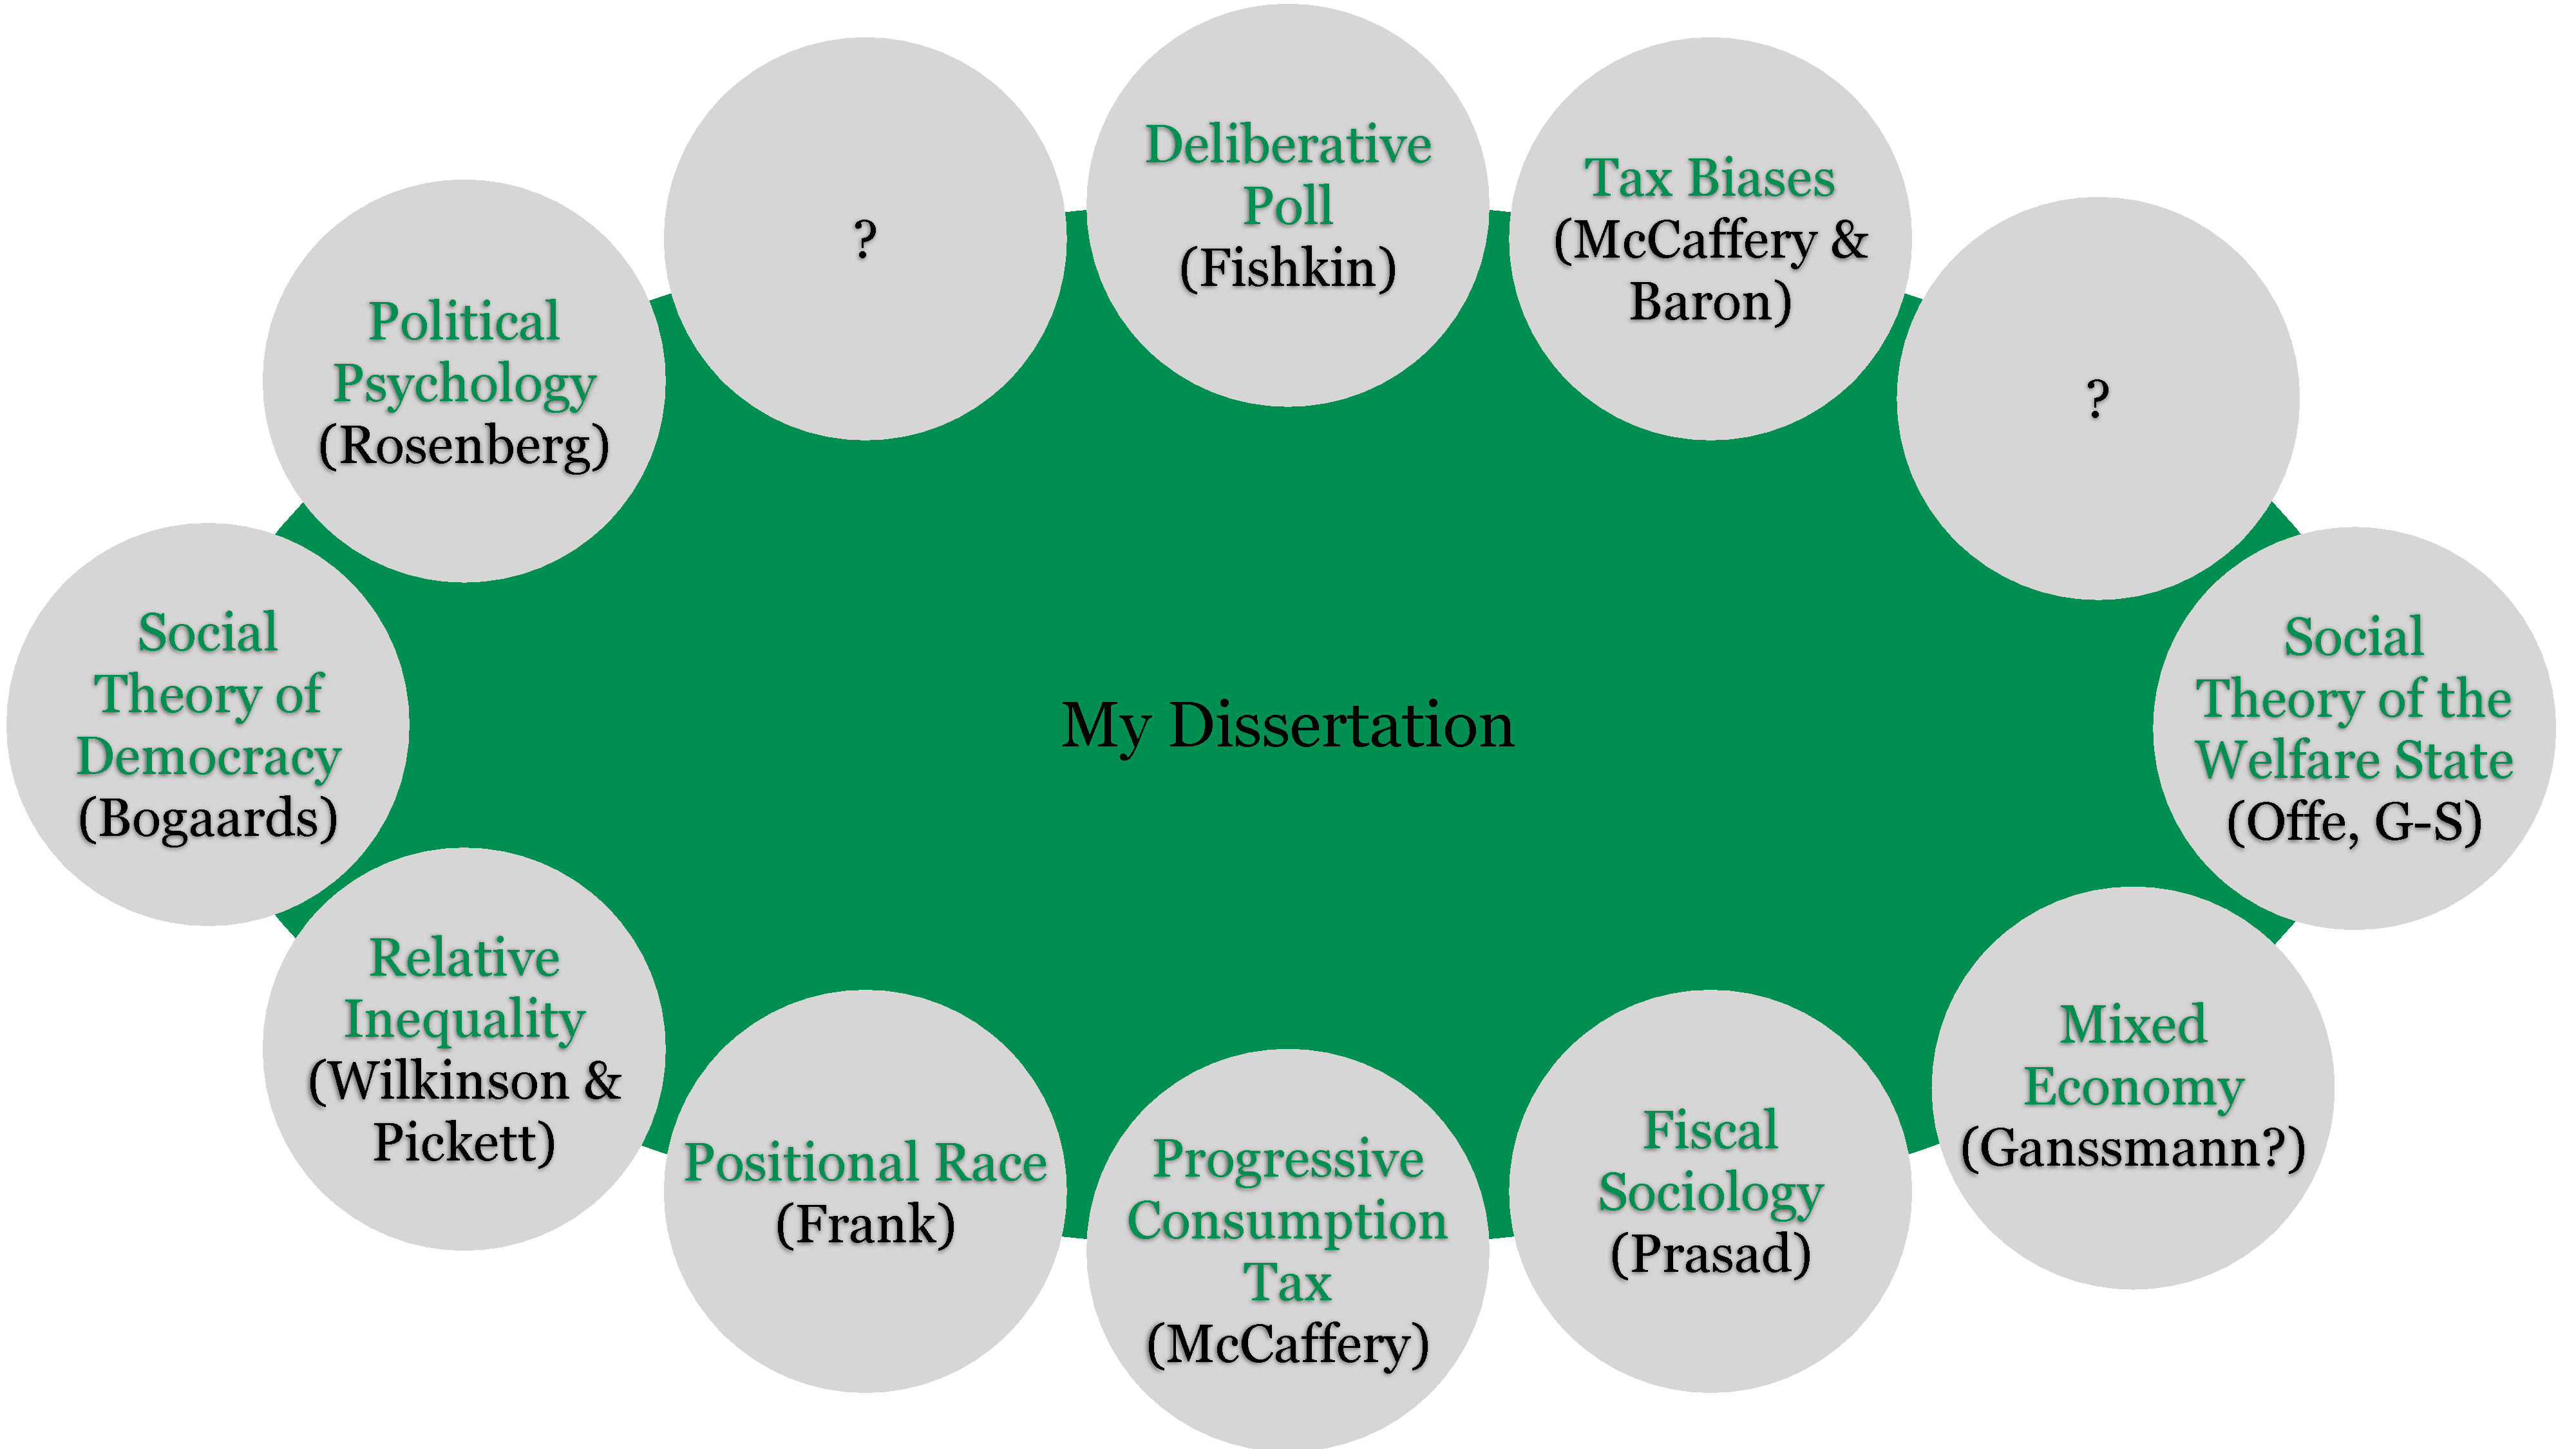
\includegraphics[width=1\linewidth]{diss-expertise}
%	\caption{Academic Fields and Advisors for this Dissertation}
%	\label{fig:diss-expertise}
%\end{figure}
%
%\begin{landscape}
%\begin{figure}[htbp]
%	\centering
%	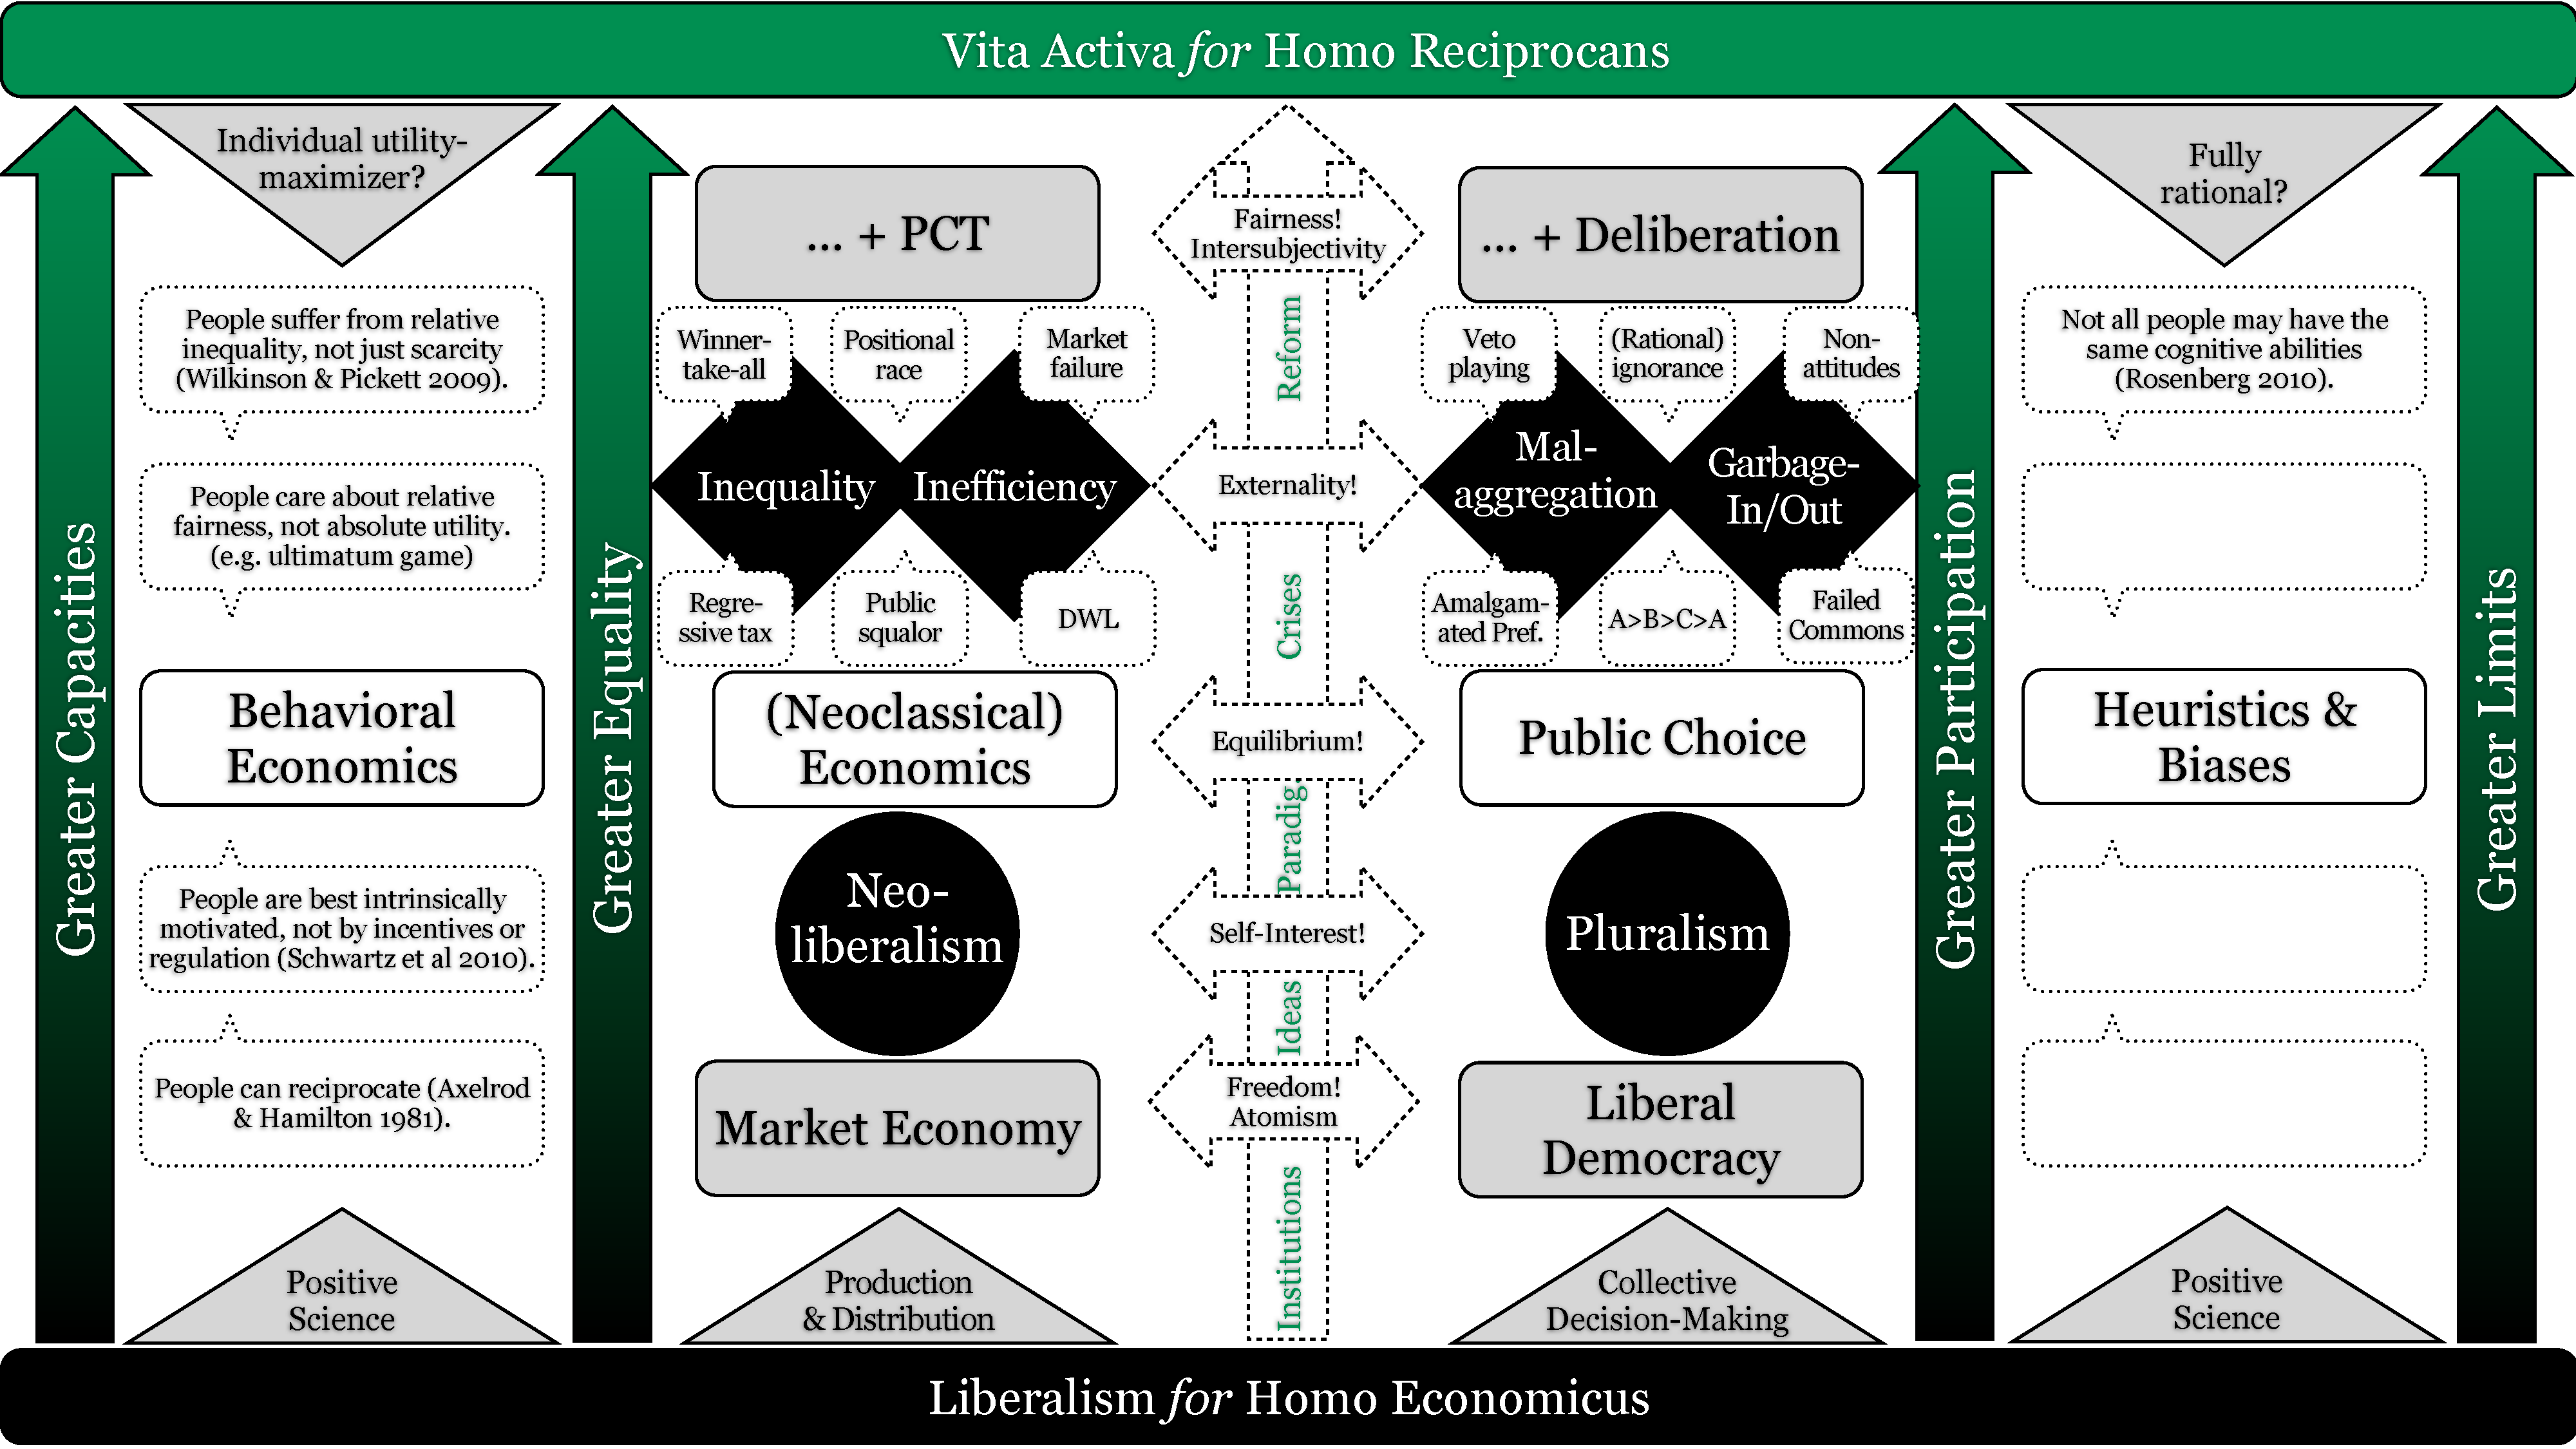
\includegraphics[width=1\linewidth]{diss-mindmap}
%	\caption{Mindmap of this Dissertation}
%	\label{fig:diss-mindmap}
%\end{figure}
%\end{landscape}

%comment MN: zwei sehr starke apriori annahmen
	%1 überlegegenes demokratisches Verfahren, politisches verfahren
	%2 überleges steuersystem
	%Aber: Ratio UND Emotion, Argument UND Narration, Gemein UND Eigeninteresse. Wieso priviligierung *eines* Pols?
\chapter*{About This Document}
	\label{chap:how2}
	%!TEX root=../tax-democracy-held.tex

\section*{How To \ldots} \label{chap:how2}

\paragraph{How to Use This Document.}
I have highlighted some words in \href{chap:how2}{green} to point to further information in footnotes, elsewhere in the document or on the internet.
In the digital version of this document, these highlights hyperlink to their respective place of finding.

I have also hyperlinked in-text citations to their entry in the bibliography.

Many of the e-books I have read do not include the original print-edition page numbers.
I reference these e-books with their (proprietary) \emph{Amazon Kindle \circledR} reading locations, identified as ``Kxxx'', such as in \citet[K50]{McCaffery2002}.
You can:
\begin{enumerate}
	\item
		Find the original source on \href{http://kindle.amazon.com/profile/Maximilian-Held/1675396}{my \emph{Kindle \circledR} account} at\\ \url{http://kindle.amazon.com/profile/Maximilian-Held/1675396}.
	\item
		Find the print-edition page number by typing the respective quote into \url{http://books.google.com}.
	\item
		Contact me to find the original source.
\end{enumerate}

\paragraph{How Not to Use This Document.}
This is an early draft of unpublished work that has not been reviewed. Please do not cite or circulate any of this.

\paragraph{Correspondence.}
Write to \href{mailto:maximilian.held83@gmail.com}{maximilian.held83@gmail.com} or see \\* \url{http://maxheld.de/contact} for more information.

\tableofcontents
\listoffigures
\listoftables
\chapter*{Commented Table of Contents}
	\label{chap:commented-toc-phd}
	%!TEX root=../tax-democracy-held.tex

\begin{longtabu}[]
%	{l
%	l
%	p{3cm}
%	p{2cm}
%	p{5cm}
%	r
%	r}
	{X[]
	X[]
	X[8]
	X[7]
	X[16]
	X[]
	X[]}

\caption{Commented Table of Contents\label{tab:commented-toc-phd}}\\

%firsthead
	\toprule

	\emph{\#}
	&\emph{}
	&\emph{Title}
	&\emph{Function}
	&\emph{Content}
	&\emph{p.}
	&\emph{\%}
	\\

	\midrule

\endfirsthead

%n-heads
	\toprule

	\emph{\#}
	&\emph{}
	&\emph{Title}
	&\emph{Function}
	&\emph{Content}
	&\emph{p.}
	&\emph{\%}
	\\

	\midrule

\endhead

\small

\emph{}
&	\ref{chap:introduction-phd}
&	\nameref{chap:introduction-phd}
&	Introduction
&	\emph{Lays out the structure of the dissertation.}

	%more text?
&	\pageref{chap:introduction-phd}
& 95
\\

\emph{}
&	\ref{chap:proposal-phd}
&	\nameref{chap:proposal-phd}
&	Proposal
&	\emph{Summarizes the planned research as a conventional proposal.}

	%more text?
&	\pageref{chap:introduction-phd}
& 95
\\

\midrule

\ref{part:puzzle}
& 	\emph
&	\nameref{part:puzzle}
&	Proposal
&	\emph{Explicates the research gap.}

	The current crises and performance of both established democracy and welfare states can only be understood, when compared with desirable and doable hypotheticals in democratic fora and tax.
&	\pageref{part:puzzle}
\\

\emph{}
& 	\ref{chap:wanted}
&	\nameref{chap:wanted}
&	Foundations
&	\emph{Lays out the structure, epistemology, ontology and axioms of the dissertation.}

	Social scientists must ask not just what \emph{is}, but what \emph{could} be (First Order Theory) and explain why it is not (Second Order Theory).
	Such hypotheticals must be desirable and doable.
	Desirable and doable are defined.
&	\pageref{chap:wanted}
& 95
\\


\emph{}
&	\ref{chap:mixed-economy}
&	\nameref{chap:mixed-economy}
&	Theoretical Background
&	\emph{Explains for which ends, and by which means market and plan can coexist.}

	Welfare states are properly understood as mixed economies, where government supplements market outcomes by coercive plan.
&	\pageref{chap:mixed-economy}
& 90
\\

\emph{}
&	\ref{chap:3-crises}
&	\nameref{chap:3-crises}
&	Empirical Background
&	\emph{References empirical and theoretical findings on the intertwined crises of democracy, the welfare state and equality.}

	Established democracies are constrained, gridlocked and confused.
	Welfare states are unsustainable and/or defunct.
	Economic inequalities are widening.
&	\pageref{chap:3-crises}
& 65
\\


\emph{}
&	\ref{chap:tax-matters}
&	\nameref{chap:tax-matters}
&	Literature Review
&	\emph{Explains how tax matters to the mixed economy, welfare state and democracy.}

	Mixed economies rely on efficient and equitable taxation.
	Democratic government always faces trade-offs in designing welfare states.
	Voters must understand these alternatives, and all materially possible designs must be available for voters.
&	\pageref{chap:tax-matters}
& 80
\\

\emph{}
&	\ref{chap:hypotheticals-matter}
&	\nameref{chap:hypotheticals-matter}
&	Critique of the Literature
&	\emph{Without appreciating doable and desirable hypotheticals, social science becomes latently affirmative.}

	This is especially true for welfare state research.
	Absent a critical comparison to a hypothetical ideal mixed economy, the second-order account of welfare fails to explain most of the current shortcomings.

	%more text missing?
&\pageref{chap:hypotheticals-matter}
&60
\\

\emph{}
&	\ref{chap:testing-hypotheticals}
&	\nameref{chap:testing-hypotheticals}
&	Research Design
&	\emph{Describes the positive research design to make the hypotheticals empirically falsifiable.}

	Under a different (deliberative) democratic process, a random sample of ordinary voters will understand the mixed economy differently and prefer a different (progressive consumption, land-value) tax.
&	\pageref{chap:testing-hypotheticals}
&65
\\

\midrule

\ref{part:tax}
&	\emph{}
&	\nameref{part:tax}
&	Theory
&	\emph{Reviews mainstream economic thinking about desirable and doable taxation.}

	The first order theory of tax asks, and answers what the most desirable, but doable tax is.
&	\pageref{part:tax}
&
\\


\emph{}
&	\ref{chap:desirable-tax}
&	\nameref{chap:desirable-tax}
&	Theory (Review)
&	\emph{Reviews mainstream economic thinking about efficiency and equity of taxation.}

	A desirable tax offers one of the higher possible trade-offs between efficiency and equity.
&	\pageref{chap:desirable-tax}
& 80
\\


\emph{}
&	\ref{chap:doable-tax}
&	\nameref{chap:doable-tax}
&	Theory (Analysis)
&	\emph{Lists factual complications and contradictions of taxation.}

	A doable tax is personal, falls on inelastic bases, has a well-defined incidence, least affects liquidity choices and is agnostic towards the source of income.
&	\pageref{chap:doable-tax}
& 85
\\


\emph{}
&	\ref{chap:better-tax}
&	\nameref{chap:better-tax}
&	Theory (Synthesis)
&	\emph{Evaluates real and hypothetical taxes on the aforedeveloped criteria of desirability and doability.}
	A \glsfirst{pct} and \gls{lvt} emerge as by far the best, most desirable and doable taxes.
	Other, existing taxes violate efficiency, equity, or both and display manifold unintended consequences and unavoidable loopholes.
&	\pageref{chap:better-tax}
& 85
\\

\midrule

\ref{part:democracy}
&	\emph{}
&	\nameref{part:democracy}
&	Theory
&	\emph{Reviews normative, theoretical and empirical political science on democracy.}

	The first order theory of democracy asks, and answers what the most desirable, but doable form of democracy is.
&	\pageref{part:democracy}
&
\\

\emph{}
& 	\ref{chap:desirable-democracy}
&	\nameref{chap:desirable-democracy}
&	Theory (Review)
&	\emph{Briefly reviews normative political theory on democracy.}

	A desirable form of democracy provides effective participation, control of the agenda, voting equality and enlightened understanding \citep{Dahl-1989-aa}.
	%MN COMMENT: sehr spezifische Sichtweise der Demokratie; wieso soll ausgerechnet das das beste an der Demokartie sein? Was ist mit power, interest, praxis?
&	\pageref{chap:desirable-democracy}
& 10
\\

\emph{}
&	\ref{chap:doable-democracy}
&	\nameref{chap:doable-democracy}
&	Theory (Analysis)
&	\emph{Briefly reviews public choice theory and political psychology.}

	Some likely micro- and macropolitical dynamics divert real existing, formally democratic government from normative desiderata.
	Doable democracies face different, sometimes unattractive, trade-offs between participation, deliberation and political equality \citep{Fishkin2009}.
	In complex societies, the dysfunctions and trade-offs may be harsher, still.
&	\pageref{chap:doable-democracy}
& 10
\\


\emph{}
&	\ref{chap:better-democracy}
&	\nameref{chap:better-democracy}
&	Theory (Synthesis)
&	\emph{Briefly reiterates the deliberative theory of democracy, and describes prominent institutional designs.}

	Deliberative democracy promises to overcome many of the trade-offs and dysfunctions of pluralist democracy, by stressing intersubjective understanding and communicative action in lieu of pre-social preferences and power in speech.
&	\pageref{chap:better-democracy}
&10
\\

\midrule

\ref{part:tax-democracy}
& 	\emph{}
&	\nameref{part:tax-democracy}
& 	Theory (Original)
&	\emph{Develops a second order theory of democratic choice of tax.}

	Deliberative democracy is a good \emph{method} to test one explanation for the absence of a better tax.
	%MN Comment: nein, keine Methode -- das ist Fishkins Fehler
	Deliberative democracy is also \emph{more} than a method:
	deliberation and \gls{pct}/\gls{lvt} are conceptually related.

	Tax is a good \emph{case} to test deliberative democracy.
	%MN comment: wieso sollten wir sie testen?
	Tax is also \emph{more} than a case:
	it is \emph{the} social contract in capitalism.
&	\pageref{part:tax-democracy}
&10
\\


\emph{}
&	\ref{chap:no-better-tax}
&	\nameref{chap:no-better-tax}
& 	Theory (Original)
&	\emph{Reviews and develops alternative second order explanations for why we do not have a better tax.}

	We may not have a better tax, because progressive taxation is plagued by a global cooperation problem, because of path dependency, because of domestic political dysfunctions or, simply, because people do not want it.
	I try to falsify only the last explanation, and theorize how different democratic processes may alter, suppress or confuse the will of the sovereign.
&	\pageref{chap:no-better-tax}
&55
\\


\emph{}
&	\ref{chap:tax-under-pluralism}
&	\nameref{chap:tax-under-pluralism}
&	Theory (Hypotheses)
&	\emph{Hypothesizes falsifiable, popular misunderstandings of tax and the mixed economy that may divert voters away from the \gls{pct} and \gls{lvt}.}

	Voters incorrectly think
	\begin{inparaenum}
		\item that a mixed economy cannot have an arbitrary savings rate,
		\item that nominal variables reflect actual savings,
		\item that a mixed economy cannot have an arbitrary state-market mix,
		\item that non-natural persons can be taxed and
		\item fail to aggregate different taxes, indirect taxes and ``social contributions''
	\end{inparaenum}.%add hrefs to the above?
&	\pageref{chap:tax-under-pluralism}
&35
\\


\emph{}
&	\ref{chap:common-grounds}
&	\nameref{chap:common-grounds}
& 	Theory (Outlook)
&	\emph{Develops conceptual and theoretical linkages between the \gls{pct}, \gls{lvt} and deliberative democracy.}

	The \gls{pct}/\gls{lvt}  and deliberative democracy embody and enforce a similar standard of justice as fairness \citep{Rawls-1971}.
	The \gls{pct}/\gls{lvt} enable the kind of equality on which deliberative democracy relies.
	The \gls{pct}/\gls{lvt} and deliberative democracy both build, and require deep cooperation.
&	\pageref{chap:common-grounds}
&15
\\

\bottomrule
\end{longtabu}
%\chapter*{Acknowledgements}
	%\label{chap:acknowledgements}
	%%!TEX root=../thesis.tex

\chapter*{Acknowledgements}

%Franziska Deutsch, who has brought me and Bogaards together, and reminded me why tax and democracy is so important (it affects everyone, but no one understands it).

%Olaf who's always shepharded this projec

%Mauricio Reichenbachs, Karin Gottschall for feedback in May 2012 (Doctoral colloquium) for chapter \ref{sec:mixed_economy}
	%This chapter benefited greatly from extensive feedback from the field 3 doctoral colloquium at the Bremen International Graduate School of Social Sciences. Special thanks to my commenters Karin Gottschall and Mauricio Reichenbachs for their thoughtful feedback in the fall of 2012.

%also to Christoph Ossege and Alexander Deutsch for CHapter \ref{sec:mixed_economy}

%to Claus Offe for reminding me that I need a second-order theory.

%   * Franziska Deutsch for getting me in touch with Matthijs Bogaards, and for providing the ultimate rationale why tax and deliberation "everyone's affected, but no one understands it
%   * Libraries.
%   * My friends and colleagues who accepted all the whining.
%   * Dr. Stephens
%   * Dr. Genschel
%   * Colloqium people
%   * Dr. Scharpf
%   * Dr. Ganghof
%   * Dr. Werner
%   * Karlhans-Sauernheimer, who gave me thoughtful comments on the MPP piece, and for getting me interested in economics in the first place.


\chapter*{Preface}
	\label{chap:preface-phd}
	%!TEX root=../tax-democracy-held.tex

\chapter*{Preface} \label{chap:preface-phd}

%This has to be an opus magnum, it will be the last. No writing after this.

%Write preamble:
%I used to be a pretty centrist, even right of centrist guy. More specifically, I used to be affirmative. I believed in the institutions that had really been very kind to me all my life. Then I looked into things. I though they were just random noise, a few mistakes in an actually more or less functional system. Turns out, that's not true.

%Not: On the shoulders of giants.
%But: I was nurtured in fertile ground, forgiven, inspired, motivated, given chances, pampered.

%IN the introduction, write about the sociology of my upbringing, how I go to be who I am. By incredible sheltering and nurturing and (petty bourgeois) privilege. Do something like Gladwell does in "Outliers".
%- 1a at Grundschule Barrien
%- Jacobs, at a time when private english-speaking universities were still new
%- the son of the judge, can always cut corners
%- Studienstiftung, SchülerAkademie, Fulbright
%- not my accomplishment
%- my challenges: ill health, Kettenhemd.
%- Bilingual high school.
%- think about when I work best (SchülerAkademie).
%- outcast, introduced socialized by band camp
%- county with one of the largest music schools (KMS DH)
%- from one of the richest countries. Must be somewhere in the upper xth percentile of income.
%make sure this doesn't sound like I think what I wrote would be absolutely brilliant (it may not be) and therefore require explanation of my brilliance.

%I have always gotten third chances.

\mainmatter
\chapter{Introduction}
	\label{chap:introduction-phd}
	%!TEX root=../tax-democracy-held.tex

\chapter{Introduction} \label{chap:introduction-phd} 

%quote missing! or do I not need one here?

%this needs to be re-arranged when the other chapters are done.

This dissertation is fairly pedestrian. 
I tread in some of the mundane minutiae of modernity; initially the twists of tax, and later the details of democratic rule. 
And yet, in that small print of the social contract, I have found a veritable crime story.

The story begins with \hyperref[part:puzzle]{a puzzle} (\autoref{part:puzzle}, p.~\pageref{part:puzzle}): why, in the richest of countries, in the most enlightened of times (current day \gls{OECD}-world) do we still find ourselves amidst \hyperref[chap:3-crises]{three intertwined crises} (\autoref{chap:3-crises}, p.~\pageref{chap:3-crises}): 
\begin{enumerate}
	\item 
		of welfare states, too constrained to elegantly improve upon the equity, efficiency and sustainability of markets,
	\item 
		of democracies, too paralyzed to meaningfully rule their economies and
	\item 
		consequently, of political equality and economic opportunity? 
\end{enumerate}
This lament alone does mean there was crime: maybe, these are no crises, but just facts of life, and a thorough investigation is unnecessary. 
Likewise, we do not call in murder police when some centenarian does not wake up one morning.
However, at least, we task a doctor to establish a cause of death. 
So it is with these three crises: before any criminal investigation can start, I must establish a causal theory for constrained welfare, paralyzed democracy and rampant inequality. 
I find that causal theory in the complex interactions of markets and plans, as they coexist in a \hyperref[chap:mixed-economy]{mixed economy} (\autoref{chap:mixed-economy}, p.~\pageref{chap:mixed-economy}). 
Specifically, I find that of the political institutions that make up an intact mixed economy, \hyperref[chap:tax-matters]{tax matters} most to welfare, democracy and equality (\autoref{chap:tax-matters}, p.~\pageref{chap:tax-matters}).
%wanted is missing.
%also, the order is wrong, but I am not sure thatÄs so bad.

This dissertation is staunchly reformist. 
Just because a system may be in crisis, it does not require a revolutionary overhaul, nor does it warrant dialectical glee about its supposed inevitability. 
I stick to the market economy \emph{and} the welfare state, and merely tinker with tax to make them coexist better, and to mutual advantage. 
There, I have found a scandal. %some chapters are missing here

Our choice of tax can only be scandalous, let alone criminal, if there is, in fact, a better tax. 
And so, in \autoref{part:tax} (p.~\pageref{part:tax}) I ask: what makes a \hyperref[part:tax]{tax} \hyperref[chap:desirable-tax]{desirable} (\autoref{chap:desirable-tax}, p.~\pageref{chap:desirable-tax}) and what makes it \hyperref[chap:doable-tax]{doable} (\autoref{chap:doable-tax}, p.~\pageref{chap:doable-tax})?
I evaluate all real and hypothetical taxes on these criteria, and find: (progressive) taxes on the (unimproved) value of land and (postpaid) consumption are much \hyperref[chap:better-tax]{better} than the ones we have (\autoref{chap:better-tax}, p.~\pageref{chap:better-tax}). 
By comparison, our existing taxes on income and (prepaid) consumption appear staggeringly inefficient, inequitable and unsustainable. %but also unfair, reference all of these adjectives.
Because the tax foundations of our mixed economies are thus sabotaged, our democracies must needlessly trade off efficiency, equity, and sustainability.

This dissertation is sociological, not just economic. 
I cannot merely posit a suboptimal choice in tax, but I must theorize and test some social process to account for the supposedly suboptimal choice in tax. 

\hyperref[part:democracy]{Democracy} is the social process that ought to rule collective choice (\autoref{part:democracy}, p.~\pageref{part:democracy}). 
It, too, needs specification: what \hyperref[chap:desirable-democracy]{should} it strive for (\autoref{chap:desirable-democracy}, p.~\pageref{chap:desirable-democracy}), and what \hyperref[chap:doable-democracy]{can} it deliver (\autoref{chap:doable-democracy}, p.~\pageref{chap:doable-democracy})? 
In the balance of these questions I find: liberal, but deliberative democracy may be much \hyperref[chap:better-democracy]{better} than the representative institutions we have (\autoref{chap:better-democracy}, p.~\pageref{chap:better-democracy}). 
By comparison, the status quo of pluralism appears to be a minimal formulation of liberal democracy, as skeptical about what people \emph{can} do, as it is restrictive about what democracy \emph{should} do. 
Once a historical achievement, it today appears hopelessly outmatched by the vast complexity and tightly concentrated special interest of late capitalist society.

So, ``who dunnit"? 
Because this dissertation is, at bottom, positivist, I cannot show what --- let alone \emph{who} --- prevented a better tax, or a better democracy.
Non-events such as as land or consumption taxation and deliberative democracy are always causally underdetermined, just as history is always overdetermined. 
For a detective, that is a bit of a let-down, but there is still work to be done. 
I might not find the perpetrator, but at least, I can absolve wrongly accused democracy, and, during the hearing, spread word of  the crime.

\autoref{part:tax-democracy} (p.~\pageref{part:tax-democracy}) investigates the link between \hyperref[part:tax-democracy]{tax and democracy}. I start by rounding up \hyperref[chap:no-better-tax]{some suspects} for suboptimal taxation (\autoref{chap:no-better-tax}, p.~\pageref{chap:no-better-tax}) and proceed --- as Holmes advises --- by the method of elimination. 
First up: democracy itself. 
Maybe, ``suboptimal'' tax is, in fact, the \emph{popular} choice. 
Only if it is not, is there a failure of the political process to be puzzled over, and accounted for. 
I suggest that tax choice depends on the \emph{kind} of democracy. 
Tax choice may suffer \hyperref[chap:tax-under-pluralism]{under pluralism}, because it is very complicated and offers tightly concentrated special interest (\autoref{chap:tax-under-pluralism}, p.~\pageref{chap:tax-under-pluralism}). 
More broadly, the two crimes of suboptimal taxation and limited democracy are intimately related. 
People might not just widely misunderstand taxation, but they might err systematically about the trade-offs of ruling a mixed economy. 
These systematic misunderstandings under the dysfunctions of pluralism might interact with the unattractive alternatives of a dysfunctional tax regime to dramatically constrain any popular choice of tax, and divert the polity away from the equity, efficiency and sustainability they might otherwise prefer. 
Democracy and taxation might be closely intertwined in their supposed mutual crises, but they also constitute two sides of the same coin that is the liberal-democratic, capitalist social contract. 
Democracy concerns the making of collectively binding decisions, taxation is the chief means to implement these agreed-upon plans within the market exchanges of free agents. 
Conversely, democracy legitimates tax and calls the trade-offs of the mixed economy, and taxation also shapes the material conditions under which people decide, and collects the resources to power policy. 
Not surprisingly, democracy and taxation share \hyperref[chap:common-grounds]{common theoretical grounds}, and their crises and reform hinge on the same questions of equality, justice, cooperation and human nature (\autoref{chap:common-grounds}, p.~\pageref{chap:common-grounds}). %cumbersome, improve wording

This dissertation is also empirical. 
To stay clear of hermetic ideology, and self-referential critique, I must get up from the normative armchair and show that really, a better democracy and better tax \emph{are} related and \emph{can} be had.

A good crime story cannot rely on conjecture alone, it needs supporting evidence. 
I cannot provide an instrument of crime because history does not leave material what-ifs in its wake. 
But I can try to capture these hypotheticals in an \hyperref[part:test]{experimental trap}: if ordinary %better wording 
people, under an \emph{alternative}, democratic process, choose an \emph{alternative}, preferable tax, \emph{that} would be as close to a smoking gun (\autoref{part:test}, p.~\pageref{part:test}) as it gets. 
If, moreover, that experimental democracy can be shown to alleviate some of the dysfunctions of pluralism, and misunderstandings of the mixed economy, and if, consequently, through that democratic fora, people prefer an alternative tax, we know for sure that \emph{some} crime \emph{has} happened. 

This dissertation is, lastly, \hyperref[part:hope]{hopeful}, despite it all (\autoref{part:hope}, p.~\pageref{part:hope}): the crime remains unsolved, and I can point to no single societal culprit. 
Maybe, that is for the better, as few good things ever come from such structuralist exorcisms. 
There may be many reasons why we have no better tax, and the \emph{kind} of democracy we have might plausibly be one of them. 
That alone ought to worry us.

If, in fact, our pluralist democracies becoming illegitimate and inefficient, their increasing failures will plague many arenas of collective choice other than taxation. 
The death knells of legitimate and efficient pluralism --- complexity and tightly concentrated special interest --- \emph{are} the conditions of late capitalist society. %they are also the good news of late capitalist society, because zero-sum transactions are bad 
I \hyperref[chap:conclusion-phd]{conclude} that taxation may just be one these policy fields in which the limits of pluralism show early, and clearly (\autoref{chap:conclusion-phd}, p.~\pageref{chap:conclusion-phd}). %broken href
Indeed, the entire story could be told the other way around, with popular rule as the corpse that found its master in the intricacies of tax.

This dissertation is fairly long and not very original. 
Others already have, in different places and with different foci, written almost all that is contained in the next \pageref{end} pages. And yet, so far, no one has bothered to connect the dots. 
That is what I offer here.

Raymond \citeauthor{Williams1992} has argued that the detective story appears at roughly the same time as sociology, and for the same reason: to penetrate the modern world, as Conan Doyle's \emph{Sherlock Holmes} does, ``by an isolated rational intelligence'' \citep[88]{Williams1992}, otherwise covered by London fogs, or compartmentalized by functional differentiation \citep{Durkheim-1893-aa}. 
And so it is with this crime story of taxation and democracy: shrouded in nebulous complexity, pigeonholed into disjunct institutions and areas of expertise, it needs a lot of detective work to connect these dots. 
To hear this case, I urge the reader to consider all of the evidence reviewed in this exposition, even if some of the detail might, at first, seem trivial. 
It is not. 
As Sherlock Holmes reminds us, ``there is nothing so important as trifles'' \citep[238]{Doyle1891}. 
From the incidence of the \gls{CIT}, the liquidity effects of taxing property to the macro- and micropolitics of democracy and the sociobiology of fairness, cooperation and equality %add hrefs
--- these ``trifles'' are all important exhibits to make the case that democracy, taxation, and with it, all our modern lives, \emph{could}, and therefore, \emph{should} be better.

Some stories just cannot be told in the short form, and the story I have stumbled upon and here report may be one of those. %include reference to the effect that books are better from Caplan 
Luckily, detective stories can also be fun to read, and so, I hope, is this one.
\chapter{Proposal}
	\label{chap:proposal-phd}
	%!TEX root=../tax-democracy-held.tex

\footnote{
	The structure follows \citeauthor{Schmitter2002}'s suggestions for a good PhD proposal \citeyearpar{Schmitter2002}.
}

\begin{quote}
    \emph{``The spirit of a people, its cultural level, its social structure, the deeds its polity may prepare --- all this and more is written in its fiscal history, stripped of all phrases.
    He who knows how to listen to its message here discerns the thunder of world history more clearly than anywhere else.''}
    \\*
    --- Joseph \citet[6]{Schumpeter}
    %add better source
\end{quote}

\begin{quote}
    \emph{``The unforced force of the better argument'':}
	%\cite[305]{Habermas1996}
	\\*
    \emph{``The speaker must choose a comprehensible expression so that speaker and hearer can understand one another.''}
    %\cite[2f]{Habermas1976}
    \\*
    \emph{``[A]nyone acting communicatively must, in performing any speech act, raise universal validity claims and suppose that they can be vindicated.''}
	%\cite[2]{Habermas1979}
	\\**
    --- Jürgen Habermas (\citeyear[305]{Habermas1996}, \citeyear[2f]{Habermas1976}, \citeyear[2]{Habermas1979}, respectively)
\end{quote}

%write one short sentence, follow with several paragraphs to explain (schmitter)
%1.
%The idea: what do you want to study?
%2.
%The reason: why do you want to study it?

%must look at q methodology, noted in \cite{Niemeyer2007}, referencing brown 1980

\section{Introduction}
If world history is still written in tax, as \citeauthor{Schumpeter} believed, the people of our democracies, too, must read and speak these codes, to live up to the emancipatory promise of modernity.
If communicative action can heal the disagreement and confusion wrought as modernity differentiated System and Lifeworld, as \citeauthor{Habermas-1984} hopes, in our discourse on tax, too, universally acceptable validity claims instead of money and power must rule to uphold our faith in liberal democracy.

I here propose to probe into one intersection of legitimate inputs and outputs of the social contract \citep[compare][]{Scharpf1997}:
the discourse \emph{on}, and economics \emph{of} tax.

I ask, how --- if at all --- do people under current democratic arrangements think and speak differently about tax, from how they \emph{would} think and speak about it, if they lived under conditions of ideal speech.
I test, how --- if at all --- do people change their thinking and speech about tax, if they participate in a democratic process that is \emph{closer} to the Habermasian ideal?
I hypothesize that --- as a result of \emph{more} ideal speech --- people will prefer different taxes, including a \gls{pct}.
	%rather than more, write closer to, more could be misunderstood

\subsection{Taxation and Welfare}
Why does taxation matter for human welfare?

As \citeauthor{Schumpeter} knew, ``in the modern world, taxation \emph{is} the social contract'' \citep[1, emphasis in original]{Martin2009a}, even though social scientists have since paid little attention to it \citep[K191]{Tilly2009}.
Tax matters especially for current \gls{oecd}-style welfare regimes, in which markets and states must co-exist \citep{Stiglitz2011}.
In such a mixed economy, government must be able to draft some privately-owned resources to serve its --- ideally democratic --- \emph{command}, without unduly altering the prices of --- ideally competitive --- \emph{exchanges} \citep[165f]{Ardant1975} (\autoref{chap:mixed-economy}, p.~\pageref{chap:mixed-economy}).
Much of modern social integration occurs in the balance of these two contrasting logics to produce and allocate resources, ``enmesh[ing] us in the web of generalized reciprocity that constitutes modern society'' \citep[3]{Martin2009a}.
State plans make the conditions \emph{for}, and set limits \emph{to} \emph{individual} action, as when government builds roads or collects sewage fees.
Conversely, market exchanges produce much of the ``fungible resources'' used for \emph{collective} choice, as when government pays road builders or procures sewage pipes \cite[4]{Martin2009a}.

Of all conceivable institutions to govern the interface of states and markets, taxation --- not price controls, not expropriation, not debt, not printing money, not tariffs --- is the most equitable, efficient and sustainable \citep{MusgThet1959,Stiglitz2011} (\autoref{chap:tax-matters}, p.~\pageref{chap:tax-matters}).
Welfare states, with their penchant for market interventions for equity, efficiency \emph{and} sustainability, especially, rely on good taxes.

%bad überleitung, the instead doesnt work
Instead, taxation everywhere in the \gls{oecd} is in crisis.
As alternative sources of economic relief --- monetary expansion and sovereign debt --- are maxed out, structural misalignments persist, and previously forestalling (asset) bubbles have burst into their days of reckoning, public revenues appear to be strictly limited by the longtime coming contradictions of current tax regimes \citep{Streeck2013}.
%not sure about this soure, must read it
The popular mixture of (progressive) income, (proportional) consumption and (regressive) payroll taxes appears to offer only harshly unattractive tradeoffs between equity and efficiency \citep{McCafferyHines2010}, as bases have shrunk and schedules flattened \citep{Ganghof2006}.
At the same time --- possibly partly as a result --- inequalities of incomes and wealth
\footnote{
	Data on the distribution of wealth is conspicuously hard to come by \citep[158]{Crouch2004} or ordinally summarized in deciles, rendering much of the inequality invisible.
}
 have widened \citep{Butterwegge,Wagner2007,Grabka2007}.

If governments cannot raise the resources necessary to meet democratic demands without incurring prohibitive costs, the social contract is fraying \citep{Crouch2004}.
%so so shource
Whichever way governments now turn, absent better tax, they will violate the post-war capitalist compact of stable, widely shared growth \citep{Pierson2002,StreeckMertens2010} (\autoref{chap:3-crises}, p.~\pageref{chap:3-crises}).
%so-so source

\subsection{Deliberation and Democracy}
Why does deliberating taxation matter for democracy?

A dysfunctional mixed economy without good taxes may produce illegitimate outputs, and, in so far as it disturbs the state-market balance of the mixed economy, violates output congruence of a democracy \citep[compare][190]{Zurn-2000-aa}.
Yet, even if experts could agree on a tax --- such as a promising, post-paid, cash-flow based \gls{pct} --- the tradeoffs involved in choosing or calibrating a tax regime are irreducibly political.
For example, experts cannot \emph{positively} inquire whether economic ``growth''
\footnote{
	More precisely, the reaping of greater non-zero-sumness from social integration \citep{Wright2000}.
}
%Even to the extent that tax choice can be left to economic a-priori or empirical analyses, of, for example, \glspl{dwl}, such expertise relies on contentious views of human nature \citep[for a review,][]{Persky1995}, and observations of nature are, in any event, devoid of moral messages \citep[43]{Gould1982}.
is in itself \emph{virtuous}, which inter-subjective aggregation would be \emph{utility-maximizing}, what \emph{deontological} rights owners have or which human \emph{relationships} should be governed by prices or command at all --- even if they could agree on any of those alternative ethics (all discussed in \autoref{chap:wanted}, p.~\pageref{chap:wanted}).
These metaphysical conundrums are reflected in very concrete, technocratic issues in taxation, including \glspl{dwl} (p.~\pageref{sec:tax-optimality}), \hyperref[sec:diminishing-marginal-utility]{diminishing marginal utility} (p.~\pageref{sec:diminishing-marginal-utility}), the \hyperref[des:structural-agnosticism]{treatment of capital income} (p.~\pageref{des:structural-agnosticism}), or \hyperref[sec:love-marriage]{joint spousal taxation} (p.~\pageref{sec:love-marriage}), respectively.
Likewise, experts cannot justify the axioms on which their (economic) analyses rest:
whether, and under which institutional circumstances we are homines oeconomici (\autoref{chap:wanted}, p.~\pageref{chap:wanted}), cannot be exhaustively answered from observation, because nature offers no intelligible moral messages on what kind of man we \emph{should} be \citep[43]{Gould1982}.
This ontological stance matters for tax, too:
for an expert to model a general equilibrium is to invoke, as well as to make, a homo economicus.

Of all conceivable institutions to resolve these disagreements, deliberative --- not aggregative, not pluralist, not participatory --- democracy offers the greatest normative appeal, because these disagreements raise, in \citeauthor{Habermas-1984}'s words, competing \emph{validity claims}, in need of argumentative redemption, as in:
is ``growth'' \emph{comprehensible}, who \emph{truly} bears a \gls{cit}, is homo economicus \emph{right}, and are social insurance employer co-payments \emph{truthful}?
I illustrate further more, and less valid claims on taxation in \autoref{tab:validity-claims-tax} (p.~\pageref{tab:validity-claims-tax}.
%I illustrate further more -- language does not work

%!TEX root=../thesis.tex 

\begin{landscape}
\footnotesize
%\begin{longtabu}[]{p{1cm}p{2.7cm}p{3cm}p{3cm}p{3cm}p{3cm}p{3cm}} 
\begin{longtabu}[]{X[2]X[2]X[2]X[2]X[2]} 
\caption[Tax Validity Claims]{Hypothetical Examples of More and Less Valid Claims in Taxation\label{tab:validity-claims-tax}}\\
%\small

\toprule 

\emph{} 
&\emph{Comprehensibility} 
&\emph{Truth}
&\emph{Thruthfulness}
&\emph{Rightness}
\\  
	
\midrule 

%\nameref{chap:wanted}: \nameref{sec:epistemology}
%&
%&
%&
%&
%\\
%
%\nameref{chap:wanted}: \nameref{sec:axiology}
%&
%&
%&
%&
%\\
%
%\nameref{chap:wanted}: \nameref{sec:ontology}
%&
%&
%&
%&
%\\

%\nameref{chap:mixed-economy}: \nameref{sec:ends}
%&
%&
%&
%&
%\\
%
%\nameref{chap:mixed-economy}: \nameref{sec:means}
%&
%&
%&
%&
%\\

\nameref{chap:desirable-tax}: \nameref{sec:tax-optimality} (p.~\pageref{sec:tax-optimality})
& 
	\st{``A deadweight loss occurs if otherwise pareto-improving exchanges do not occur''.}
	
	``Taxes can sometimes prevent people from trading things on the market, which they otherwise would have exchanged to at least mutual benefit.''
& 
	\st{``Taxes are anti-growth''.}
	``Under some circumstances, taxes can depress market activity without raising revenue''.
& 
	\st{``Lower taxes benefit everyone, because growth trickles down''.}
	
	``If and to the extent that people react to incentives, and that we can really compare their utility, perfect markets make some people better without hurting others, compared to how things were before.''
& 
	\st{``No one would get any work done, if all their rewards get taxed away!
	''}
	
	``It seems that markets do a good job in solving some problems, and we can, to that extent and in those domains accept that people will also be influenced by threats and rewards''.
\\

%\nameref{chap:desirable-tax}: \nameref{sec:tax-justice} (p.~\pageref{sec:tax-justice})
%&
%&
%&
%&
%\\

%\nameref{chap:desirable-tax}: \nameref{sec:tax-sustainability}
%&
%&
%&
%&
%\\

\nameref{chap:doable-tax}: \nameref{sec:tax-incidence} (p.~\pageref{sec:tax-incidence})
& 
	\st{``The tax burden is distributed according to the relative price elasticities of sellers and buyers in any given taxed transaction.''}
	The ultimate burden of a tax may differ from who nominally pays it.
	Taxes are almost always levied on some trade, and their ultimate burden is distributed among the traders according to how sensitive they are to price changes.
	The less you can react to a price change, the more of a tax you bear.
&
	\st{``With a Financial Transaction Tax (FTT), we can take back the money from those who caused the financial crisis.''} %gls for FTT does not work
	
	``To the extent that a FTT discourages short-term trades, it does not raise any revenue.
	To the extent that a FTT raises revenue, behavior does not change.
	The burden of a FTT will be complexly determined by relative elasticities.''
&
	\st{``Employers already pay half of social insurance''.}
	
	``Social insurance is a payroll tax and falls entirely on labor, no matter the nominal distribution.
	The burdens are shared between employers and employees according to their relative price elasticities.''
&
	\st{``Big corporations should pay their fair share''.}
	
	``Corporations are not moral subjects; they should not be liable for redistributive or general revenue taxes.
	However, the rich people who hold a lot of stock in corporations should pay taxes on such income, or wealth.''
\\

%\nameref{chap:doable-tax}: \nameref{sec:tax-elasticity}
%&
%&
%&
%&
%\\
%
%\nameref{chap:doable-tax}: \nameref{sec:tax-schedule}
%&
%&
%&
%&
%\\
%
%\nameref{chap:doable-tax}: \nameref{sec:tax-timing}
%&
%&
%&
%&
%\\

\bottomrule
\end{longtabu}
\end{landscape}

Liberal democracy, borne out of the hope that material inequality and political autonomy \emph{can} be reconciled, %need quote
especially, rests on deliberation, because if anywhere, it is in taxation that money and power may have replaced language to govern meaning and action \citep{Habermas-1971}.
In fact, if you wanted to hide some process of (re)producing inequality anywhere, you could hardly find a better place than the intricacies of (income) taxation (consider, for example ``tax planning 101'' in \citealt[888]{McCaffery2005}).

Instead of communicative action \citep{Habermas-1984}, what emerges today from citizens, their legislatures and public spheres, may be more ``analytic muddle of tax'' \citep[862]{McCaffery2005}.
%language does not work!
The beliefs held and issues considered in the public \citep[for example,][]{Caplan2007}, appear to bear little resemblance to the abstractions suggested by economists \cite[for example,][]{Harberger1974}.
People seem to ignore fundamental choices in tax \citep[for example,][]{McCafferyHines2010}, and may fall for inconsequential alternatives \citep[for example,][]{SausgruberTyran2011}, possibly even err systematically against their own material interest --- if they are on the lower economic rungs \citep[for a German example,][]{Kemmerling2009}.
Here, too, (input) congruence of democratic rule may be violated if and to the extent that people are confused about policy choices \citep[compare][90]{Zurn-2000-aa}.

These two crises --- an ineffective and/or inefficient welfare state and a confused democracy --- may partly reinforce one another into one perfect storm of societal reaction by stealth:
\begin{quote}
	%Great argument for why tax and democracy matter:
	\emph{
	%``The two issues, the crisis of egalitarian politics and the trivialization of democracy, are not necessarily the same.
	%Egalitarians might say that they do not care how manipulative of democracy a government is, provided it divides society's wealth and power more evenly.
	%A conservative democrat will point out that improving the quality of political debate need not necessarily result in more redistributive policies.
%But at certain crucial points, the two issues do intersect [\ldots].
	``My central contentions are that while the forms of democracy remain fully in place --- and today in some respects are actually strengthened --- politics and governments are increasingly slipping back into the control of privileged elites in the manner characteristic of pre-democratic times;
	and that one major consequence of this process is the growing impotence of egalitarian causes.''}
	\\*
	--- Colin \citet[6]{Crouch2004}
\end{quote}

\subsection{Raw and Enlightened Thinking and Speech}

I here propose to investigate a supposed difference in current, and (more) ideal speech thinking about tax by subjecting a group of diverse citizens to a deliberative forum on the topic, which, in one succinct summary \cite[25ff]{Steenbergen2003}, is marked by
%\begin{enumerate}
%	\item reasonably accurate and complete \emph{information},
%	\item substantive \emph{balance} of possibly competing arguments and perspectives presented,
%	\item \emph{diversity} of participants and their positions taken,
%	\item a sincere weighting of arguments by participants, or \emph{conscientiousness}
%	\item equal consideration of all arguments, regardless of which participant offered them \cite[K1799]{Fishkin2009}.
%\end{enumerate}

\begin{enumerate}
	\item open \emph{participation}, including setting the agenda and deciding on procedures (\citealt{Benhabib-1996-aa}, \citealt{Chambers1995}, \citealt{Cohen-1989-aa}, \citealt[370ff]{Habermas1992})

	\item mutual \emph{justification} of assertions and validity claims \citep[370]{Habermas1992},

	\item orientation on the \emph{common good} \citep{Rawls-1971},
	%	\footnote{
			%not sure about this, it's kind of downstream to Habermas
	%	}

	\item \emph{respect} of one another, as well as one's arguments (\citealt{Gutmann1996}, \citealt{Macedo1999}), other-directedness, empathy and solidarity,

	\item \emph{constructive politics} of a widely acceptable decision over well-defined policy alternatives, ideally --- though not necessarily --- by consensus \citep[23]{Cohen-1989-aa},

	\item \emph{authenticity} in sincere, not strategic communication \citep[149]{Habermas-1984},
\end{enumerate}

Such a difference $\Delta$ between ``raw'' and ``enlightened'' thinking, %cite mccaffery
beliefs \citep{Caplan2007} and preferences \citep{Fishkin2009} is worth knowing for several reasons:
\footnote{
	\cite{PrzeworskiSalomon1995} suggest to explicate what readers are going to learn as a result of the proposed project, and why that would be worth knowing.
}
\begin{enumerate}
	\item There may be \emph{agreeable}, doable but hypothetical taxes, which may (Pareto)-improve over current taxes \citep{Harberger1974} or may be fairer \citep{Rawls-1971} and more sustainable \citep{Solow1956}, including a \glsfirst{pct} \citep{Mill1848,McCaffery2002,Frank2005a,Seidman1997}, a \glsfirst{lvt} \citep{George1879,Buiter1988} and a \glsfirst{nit} \citep{Friedman1962}.
	By comparison, existing taxes
	\footnote{
		In the \gls{oecd}-world, those are varying combinations of pre-paid, proportional consumption taxes such as \gls{vat} and income taxes, often with different schedules for labor, capital and corporate incomes.
		Wealth taxes, often only on some asset classes, exist in some jurisdictions, but --- with the exception of local US property taxes --- are not a large revenue source.
	}
	appear unnecessarily wasteful, inequitable and unsustainable.
	These suboptimal tax regimes may present democratic sovereigns with needlessly harsh tradeoffs between efficiency, equity, sustainability and other competing ends.
	The means of an intact mixed economy \citep{MusgThet1959,Stiglitz2011} may consequently erode or even force retrenched welfare states into ``permanent austerity'' \citep{Pierson2002,StreeckMertens2010} as it becomes harder for them to reconcile planned allocation and market exchange through taxation.

	Public confusion about taxation may be a contributing factor, or even a sufficient --- but not a necessary --- condition for the non-existence of these supposedly superior taxes.

	\item Progressivity in tax, especially, may hinge upon an enlightened, ``new understanding of tax'' \citep{McCaffery2005}, as the historic mainstay of redistribution --- the \gls{pit} --- withers away in the face of its inherent contradictions \citep{McCafferyHines2010}.
	People may understand tax \emph{systematically} different from how they would under (more) ideal speech, which may cause them to choose less effectively progressive taxes than they otherwise might, or otherwise inadvertently act even against their material self-interest.
	Additionally, the difference between raw and enlightened thinking about tax may, in itself, depend on the socio-economic status of citizens.
	Taken together, such socially structured and structuring differences in understanding tax may contribute to further, or perpetuate existing social inequality, even under nominal political equality.

	\item The aggregative and representative institutions of liberal-pluralist democracy may be partly outmatched by the vexing complexity \citep{Merton-1968-aa} and tightly concentrated interest \citep{Olson-1971-aa} of late market economies, such as in taxation, violating both their input and output legitimacy \citep{Scharpf1997} as well as basic democratic prescriptions for ``enlightened understanding'' \citep{Dahl-1989-aa}.
	Empirical political sociology bears out such popular dissatisfaction, not with democracy it self, but with incumbents, enamored by special interest, and inattentive to the public good \citep{NyeJr.1997,Norris2011,PutnamPharr-2000-aa}.
	If such a ``post-democratic'' constellation \citep{Crouch2004} were to plague the polity in its thinking about tax, it may well affect other policy areas too.
\end{enumerate}

\section{State of the Field}
This positive aspect of this thesis sits at the intersection of three fields of empirical research:
\begin{enumerate}
	\item Practical experiments with different deliberative fora on varying policy areas,

	\item Political psychology on limited and socially structured cognitive competences and

	\item Experimental and survey research about popular understandings of tax.
\end{enumerate}

In the following, I briefly report key findings from these two fields and identify avenues for further research.

\subsection{Empirical Deliberation}

\subsubsection{Deliberative Experiments}
Deliberative fora have been tried on a number of policy areas and places, including renewable energy in Texas (USA) \citep{LehrGuild-2003-aa}, participatory budgeting in Porto Allegre \citep{CoelhoPozzono-2005-aa} (Brasil), nanotechnology \citep{Powell2008}, electoral reform in British Columbia (Canada), policing and education in Chicago (Illinois) \citep{WarrenPearse-2008-aa}, and city planning in Philadelphia (Pennsylvannia) \citep{Sokoloff2005}.
They also vary in their institutional design \citep[reviewed in][]{Fung-2003-ac}.
These include several small-n, multi-day designs, such as Citizen Juries \citep{SmithWales-2000-aa} or Planning Cells \citep{Dienel-1999-aa}, where a few randomly selected citizens hear expert witness and deliberate amongst themselves for a couple of days, all facilitated by trained, non-expert moderators and prepared by a balanced briefing book to draft a Citizen's Report or similar consensus recommendation.
The otherwise similar Consensus Conferences \citep{Einsiedel2000} are often (much) longer, feature extended learning periods and are typically held on highly technical issues.
\footnote{
	Consensus Conferences were first developed and hosted in Denmark by the Technology Assessment Board to collect informed popular input for regulating science and technology.
}
Deliberation has also been tried in large-n, shorter designs with a more quantitative methodology in \gls{dp}s \citep{FishkinFarrar-2005-aa}, where hundreds of randomly selected citizens receive issue books, deliberate in small, moderated groups and plenary sessions, hear expert witnesses and --- instead of reaching a consensus --- cast a secret vote or fill out a questionnaire, after the typically daylong deliberation concludes.
Often, these survey results are compared to answers provided by participants before the event, and/or to a control group of non-participants, allowing quasi-experimental within-subject or between-subject statistical inferences.
\footnote{
	Because participants can always drop out at will and will know when they are in the treatment condition, treatment cannot be strictly randomly assigned.
}
There is quite limited experience with long, large-n designs, including --- to my knowledge --- only the \glsfirst{ca} \citep{WarrenPearse-2008-aa} that spanned several months, and included several hundred participants who were offered stipends and accommodation, participated in extended learning sessions, attended public hearings and ultimately agreed to recommend a new electoral system (a \gls{stv}) for the province \citep{Citizen-2004-aa}.

%include tables from google doc.

Across these different designs and purposes, deliberative fora have been shown to improve knowledge of the subject matter in question, to change --- but not bifurcate --- beliefs \citep{Fishkin2009}, to yield more orderly and orthogonal preferences structures \citep{Farrar2003} and to boost a sense of political efficacy or mutual trust even among disempowered citizens \citep{Karpowitz2009}.

These encouraging findings on the capacity of deliberation to strengthen democratic rule notwithstanding, much of deliberative practice may be criticized for often focusing on the immediate, tangible and remaining ``confined to the realm of neighborhood and locale'' \citep[17]{FungWright-2001-aa}.
This includes not only the overtly ``human-scale'' democratic efforts \citep[759]{Boggs-1997-aa} of participatory budgeting \citep{Sousa-Santos-1998-aa}, city planning \citep{Sokoloff2005} or public stewardship of forests \citep{Cheng2005}, but also the much-lauded \glspl{dp}, which have, even when they were about clearly large-scale issues such as the \gls{eu} \citep{Fishkin2009} or renewable energy use \citep{LehrGuild-2003-aa} mostly shied away from the very structured choices and remote abstractions which policy must engage.
These \glspl{dp} have, for example, demonstrated that more people prefer \gls{eu} enlargement and more people would be willing to pay a premium for renewables \citep[157]{Fishkin2009}, but did \emph{not} ask --- and probably not deliberate on, either --- whether the \gls{eu} was an \gls{oca}, and if not, what fiscal complements might have to be implemented \citep[for example,][]{Mundell1961}, or by which process \emph{competing} renewable energies should be chosen, especially if they depend on economies of scale and network effects \citep[for example, ][]{Krugman-1990-aa}.
Clearly, these are only two haphazardly selected examples of abstractions (\gls{oca}) and choices (infant industry regulation) relevant to these topics, but equally clearly, someone, somewhere in the democratic process has to make these calls.%fishkin quote in the above is K2010
Some of these more technocratic considerations may be rightly relegated to experts, but for others --- including the abstractions of tax --- this may not be possible or desirable as discussed in the above.
In terms of \citeauthor{Landwehr2010} \glspl{dp} may not be sufficiently ``coordinative'' to be fully deliberative, and not only because they do not enforce a collectively binding decision \citeyearpar[377]{Landwehr2010}.
Absent abstractions, ``coordinativeness'' suffers because the policy options (for example, ``faster \gls{eu} expansion'') in which preferences are expressed \citeyearpar[375]{Landwehr2010} are ill-defined (for example, \emph{what kind} of european integration?).
If such expressed preferences are allowed to detach from ontologically given policy options (for example, currency union with our without fiscal complements), people can effectively ``exit'' from substantial agreement \citep[377]{Landwehr2010}:
``deliberators'' can just talk, which may still be desirable, but stretches the concept too thin \citep[502]{Thompson2008}.
%Or, in the words of \cite[2]{Moore2011} ``the broadly democratic idea that people ought to have equality of opportunity to contribute to deliberation on matters that affect them is undermined by the huge and manifold inequalities in knowledge that are necessary for the effective analysis, regulation and management of complex social and technological problems''

To show its stripes --- or limits (!) --- deliberative democracy must be tried on such highly structured choices and abstract issues, too.
So far, with the notable exception of some Danish (small-n) Consensus Conferences and the (large-n) \gls{ca} \citep[on its complexity,][]{Blais2008}, such applications are lacking in empirical experiments with deliberation.
If deliberative practice continues to blank out governing abstractions and structured choices --- the very stuff of the modern world and its political rule --- it risks moving ``in a defensive and insular direction, laying bare a process of conservative retreat beneath a facile rhetoric of grassroots activism'' \citep[759]{Boggs-1997-aa}.
\footnote{
	A comically naive example of such retreat comes from  Piombino, Italy, where schoolchildren were ``involved'' (sic!) in urban renewal of the town piazza:
	\begin{quote}
		``After school trips (\ldots) they had to make drawings of how the piazza should look.
		These often very colorful and joyful drawings were exhibited and also put on the website of the town.''
	\end{quote}
	Praises \citet[29]{Steiner2012}:
	``In this way, children learned a good lesson about practical politics with a very concrete case of policy-making'' (sic!).
	These and other exercises in ``involvement'' may be pedagogically or otherwise valuable, but \emph{emancipatory} deliberation they are not.
	In fact, the example of children seems awfully revealing as an operative metaphor for this kind of ``deliberative'' citizen:
	let them draw cute pictures, or busy themselves with otherwise inconsequential activities, so that they feel heard.
}
%in a different, more positive vein, \cite[4f]{Boswell2013} describes such deliberative designs as concerned with `` `low politics', where the stakes are lower, the glare of publicity less pronounced and the local knowledge of citizens more prized.

\subsubsection{Academic Reflection}
These and other deliberative fora have also received ample academic reflection.

One strand of positive research treats deliberation as the \emph{independent} variable, investigating its effects (including \citealt{Bachtiger2005} on legislatures, \citealt{Hibbings2002} on power differentials or \citealt{Jackman2008} on better-grounded judgements) %fishkin 1991, niemer 2002, Hansen 2004, Schneiderhahn und Kahn 2008 all do effects
In a similar vein, \cite{Steiner2004} studied in how far deliberatively reached decisions ``correspond to criteria of social justice'' \cite[13]{Steiner2012}, by which they seem to mean a utilitarian maxim \citep{Bentham1789} or the \citeauthor{Rawls-1971}ian difference principle \cite[95]{Steiner2012}.
\footnote{
	\citeauthor{Steiner2012} presents a questionable summary of \citeauthor{Rawls-1971}:
	``This principle states that in a political decision the most disadvantaged social groups should profit the most'' \citep[95]{Steiner2012}.
	He finds it expressed when a parliamentarian says:
	``The government's priority must be to help those who have the greatest difficulty in paying rather then spreading it evenly across the range.''
	The difference principle actually states that ``social and economic \emph{inequalities} are to [\ldots] be to the greatest benefit to the least advantaged members of society'' \cite[266]{Rawls-1971}, a complex and conditional claim to moral validity that is characteristically degraded in both the operationalization and the coded snippet.
}

In other work, deliberation is the \emph{dependent} variable, investigating its causes (including \citealt{Steiner2004} on institutional aspects or \citealt[13]{Steiner2012} on issue polarization).
Similarly, \cite{Landwehr2010} compare how the \emph{discursiveness} and \emph{coordinativeness} of parliamentary debates and citizen conferences on regulating embryonic stem cell research impacts resultant preference change, their proxy for deliberation.
Employing a more sophisticated and theory-grounded operationalization than most, \citet[377]{Landwehr2010} analyze speech acts to code for arguing (for example, ``to claim'') and bargaining (for example, ``to offer'').%developed in Holzinger 2001, also Niemeyer.

Lastly, researchers simply seek to operationalize deliberation.
For instance, \cite{Stromer-Galley2007} suggests a coding scheme, including ``reasoned opinion expression'' when people provide ``a definition, a reason for holding the opinion, an example, a story, a statistic, or fact, a hypothetical example, a solution to the problem, further explanation for why the problem is a problem, an analogy, [\ldots] or any further attempt to say what they mean or why they have taken the position that they have''.

These academic reflections all try to abstract away the substantive issues at stake in the respective deliberative encounters.
Social scientists, here, as often, are loath to get caught in first-order conflicts over, say, school policy:
``[\ldots] measuring the factuality or quality of reasoning was deemed unnecessary'' \cite[10]{Stromer-Galley2007}.
This impulse is understandable, even commendable:
Social scientists are, by definition, in the business of explaining the second-orderd social conflict \emph{over} normative and positive first-order questions \citep[12][compare]{GutmannThompson-2004-aa} and must generalize from the particular to build or test social theory.
Yet, since deliberation is a \emph{discourse} ethic \citep[153]{GutmannThompson-2002-aa}, it is difficult to analyze without the actual, domain-specific discourse.
The operationalizations employed vary widely, ranging from the crudely statistical \citep{Steiner2012}
\footnote{
	Summarizes \citeauthor{Steiner2012}:
	``It is noteworthy that of the 1,027 speech acts, only 5 were interrupted by other participants, which indicates a calm and not boisterous atmosphere during the experiments'' \citeyearpar[47]{Steiner2012}.
	}
to the quick-and-dirty semantical \citep{Steiner2012}
\footnote{
	``[O]ur \gls{dqi} defined a sophisticated level of justification as having a certain complexity in the sense that an argument is justified with more than one reason and that these reasons are logically linked with the postulated outcome'' \cite[64]{Steiner2012}.
}
to promisingly speech-act linguistic \citep{Landwehr2010}.

The \gls{dqi} --- even in \citeauthor{Steenbergen2003}'s more exacting formulation --- and other such operationalizations ``can be applied easily and reliably to a wide range of deliberative contexts'' \citep[22]{Steenbergen2003}, but that very decontextualization makes it hard to adjudicate whether really, universal validity was discussed, let alone reciprocally acclaimed.
I share the uneasyness of ``critical theorists and postmodernists'' \cite[11]{Steiner2012} with this measure of quality of deliberation --- though I do not think you have to be either to object, nor for the same reasons.
\footnote{
	\cite{King2009} criticizes that coded interpretations are presented as objective fact, rather than inter-subjective.
}
Rather than \emph{how many} justifications where given in total, or \emph{how often} people referred to counterarguments \cite[29]{Steenbergen2003}, I want to know whether these reasons corresponded in \emph{substantive terms to those they disagree with}.
I provide a hypothetical exchange from deliberating taxation to illustrate my point:

\begin{dialogue}
	\speak{Foundationalist}
	\footnote{
		Inspired by the Philosophy of Robert \cite{Nozick1974}.
	}
	I believe that everyone should be entitled to incomes generated from uncoerced exchange with others.

	\speak{Social Democrat}
	\footnote{
		Not very inspired, and by no one in particular.
	}
	Yeah, obviously we are not going to take away all of a person's income, they should be entitled to it, but maybe we'll take some of it because we need that for education.
	That's not going to hurt them.

	\speak{Georgist}
	\footnote{
		Inspired by the Philosophy of Henry \cite{George1879}
	}
	I agree there may be something inviolable about owning the value added in free exchange with others.
	But, Foundationalist, do you think that should also extend to owning unimproved land and natural resources?
	It seems to me that \emph{no one} has really created these values, and whoever reaps rents from them does so \emph{only} because of the coercive powers that be.
\end{dialogue}

Formally speaking and under \gls{dqi} coding, both Social Democrat and Georgist refer to Foundationalist's argument, yet their speech acts are of strikingly different quality.
Social Democrat, rather sloppily, reiterates the argument and proceeds to balance it with another good (education) and suggests a compromise.
We can see how the dialogue would proceed;
Foundationalist --- presumably deontologically bound to inviolable property --- would refuse to trade off property against opportunity.
Talking past one another, Social Democrat and Foundationalist may not have exchanged, let alone agreed on universal validity claims.
By contrast, Georgist --- maybe provisionally --- embraces the foundationalist's argument and points to an unexpected implication \emph{in foundationalist} terms.
It is much harder to see how their dialogue would proceed;
presumably, Foundationalist would not --- ex ante --- have been open to large-scale land reform or taxation (as Georgism implies), and may not much warm to the idea.
Still, she may find it necessary to either clarify her position further, or to concede Georgist's point, because his may just be the ``forcelessly forceful'' better argument.
Foundationalist and Georgist are grappling with the formulations and implications of what \emph{may} become a universally acceptable moral claim, and in so doing, have crept a little closer to communicative rationality.

Crucially, this kind of Habermasian adjudication cannot be done in the abstract;
researchers have to look for ideal speech in \emph{substantive} terms as in this case, a foundationalist theory of property.

By abstracting away the actual arguments from a normative theory vested in their force, these researchers, as \citeauthor{Steiner2012} concedes, ``take the position that large parts of the Habermasian version should be relaxed'' \citep[150]{Steiner2012}.
For \citeauthor{Steiner2012}, ``the crucial point should be that participants in a political debate acknowledge that others also have reasonable arguments
[\ldots]
If this is accomplished, the other side is humanized'' \citeyearpar[150]{Steiner2012}.
This may well be true and important research, especially for divided societies on which \citeauthor{Steiner2012} here reports, but it stretches the concept of \emph{communicative action} too thin.

To be sure, there may be such a loosely-defined thing as ``deliberation'' --- distinct from ``debate''and ``discussion''  \citep[384]{Landwehr2010} --- and we should study its antecedents and consequences, as much of the above-cited research does.
In this vein, deliberation raises positive questions:
What ``middle-range theories'' associate antecedents and consequences \citep{Mutz2008}?
To the extent that this deliberation is a normative project at all, it espouses a \emph{consequentialist} outlook:
deliberation is good, because it leads to ``more public-spirited attitudes;
more informed citizens;
greater understanding of sources of, or rationales behind, public disagreements;
a stronger sense of political efficacy;
willingness to compromise;
greater interest in political participation;
and, for some theorists, a binding consensus decision'' \citep[524]{Mutz2008}.

Habermas prescription for communicative action, again, is different.
Communicative action is not a positive statement about causes and effects open to falsification, because it poses a \emph{regulative} principle \citep{Kant1781}, which ``is unachievable in its full state, but remains an ideal to which, all else equal, a practice should be judged as approaching more or less closely'' \cite[80]{Mansbridge2010a}.
Communicative action is also not a consequentialist ethic, but deontological, because ``it has the force to legitimate'' \citep[147]{Habermas2008} --- or even teleological, because ``reaching understanding is the inherent telos of human speech'' \cite[287]{Habermas-1984}.
As such a normative political theory, communicative action cannot be operationalized into a set of treatments.
Just because you subtract power, inequality, disrespect \citep{Steenbergen2003}, even ``irrationality'', or any other combination of procedural criteria from communication  does not necessarily make it ideal speech --- even though the inverse may well be true, as these and other criteria may be \emph{necessary} conditions for ideal speech.
Legitimating collective choice through ideal speech \emph{is} the irreducible, final reason of \citeauthor{Habermas-1984}' political theory whose achievement can only be found in substantive arguments.

Still, to thereby ``simply define'' deliberation as ``intrinsically good'' does not, as \citet[524]{Mutz2008} suspects, render ``empirical research irrelevant''.
As \citet[13]{Steiner2012} reminds us, the ``level of deliberation'' must be ``measured and not merely assumed''.
By definition, the normative impetus of communicative action cannot be falsified, but we may find that at any given time, any given people under any given circumstances, \emph{fail} to meet Habermas' exacting standards \citep[499]{Thompson2008}.
Such failures can serve ``as indicators of \emph{contingent} constraints that deserve serious inquiry and [\ldots] as detectors for the discovery of specific causes for existing lacks of legitimacy'' (\citealt[420, emphasis in original]{Habermas2006}, compare also \citealt[502]{Thompson2008}).
	%Indeed, empirical researchers ``should focus on those features of the practice that directly relate to the fundamental problem deliberative theory is intended to address: In a state of disagreement, how can citizens reach a collective decision that is legitimate?'' \cite[502]{Thompson2008}.

If we accept this more demanding definition of deliberation as the venue in which our approximating of ideal speech is ascertained, as I here wish to do, our research designs must be focused on argumentative substance.
Others have done this, and have produced encouraging insights.
\cite{Ratner-2008-aa} interviewed \gls{ca} members after the fact, and found that most members considered Habermas' validity claims honored --- especially compared to the proper tragedy that was the following referendum campaign in which many \gls{ca} alumni participated.
While the analysis is based on interviews, not process data, it maintains the Habermasian standard and does not spare the reader qualitative data, including snippets recounting substantive disputes over electoral design.
\cite{GutmannThompson-2004-aa}, too, reporting on deliberations over medical rationing, stick to their (quasi-Habermasian) standard, argumentative reciprocity, and offer examples of how it is met or violated in substantive arguments over health care.

Some may object that this approach collapses the procedural theory of democracy into a substantive theory of justice, and that it consequently requires researchers to take sides.
This neither need, nor ought to be so.
\citeauthor{Habermas-1984}' \emph{Communicative Action}, much like \citeauthor{Rawls-1971}' contemporary \emph{Theory of Justice} is neither purely procedural, nor substantive, but elegantly posits the \emph{discursive conditions} under which substantive claims ought to be made.
The contrast between procedural and substantive theory, here, as elsewhere, is misleading:

\begin{quote}
	\emph{``This kind of public philosophy would avoid the dichotomy that has come to dominate contemporary discussions of political theory, which poses a choice between basing politics on a comprehensive conception of the good, on the one hand, or limiting politics to a conception of procedural justice, on the other.
	We can and should avoid choosing either of these approaches exclusively''}\\*
	--- \citet[90]{GutmannThompson-2004-aa}.
\end{quote}

Consequently, researchers need not take sides, nor follow (dubiously legitimate) expert rule \citep{Blok2007,Haas1992}.
Emphatically, ``alternative conceptions of the common good'' \citep[23]{Cohen-1989-aa} are possible and desirable.
Researchers must, however, familiarize themselves deeply with the issue to be deliberated, penetrate the discursive fluff and distortions to relentlessly unearth causal and moral disagreements which reasonable people may have over the issue.
Researchers can then analyze their rich, qualitative, ideally process data in terms of these expected disagreements, to assess in how far the observed deliberation lives up to the standards of communicative action.
Ideally, deliberators will struggle to formulate universal validity claims to express and resolve these very disagreements.
In short, researchers need not have a position on the issue, but they \emph{must have a stake} in the abstractions, disagreements and uncertainties plaguing the issue.

Communicative action on taxation, in particular, must be analyzed in substantive terms for these reasons.
Tax is fraught with deep-seated causal and moral disagreement.
To test whether people in any given deliberation on tax really have exchanged universal validity claims to --- potentially --- resolve these disagreements, their actual communication must be compared to some ideal standard of expected arguments, tentatively identified by researchers, as provisionally illustrated in \autoref{tab:validity-claims-tax} (p.~\pageref{tab:validity-claims-tax}).

%taxation is that case

\subsection{Political Psychology}
Communicative action is very demanding of the cognitive and moral faculties of deliberators.
Political psychologists have problematized these demands that deliberation poses \citep{Rosenberg-2002-aa} --- especially, but not only, deliberation of highly abstract topics.
Troublingly for deliberative democracy of the Habermasian kind, recent research in political psychology suggests, that --- contrary to the bounded rationality assumption \citep[for example,][]{Simon-1999-aa,Kahneman2011} --- imperfect human reasoning may not only stem from remediable cognitive scarcity, but may be developmentally determined.
\citet{Rosenberg-2002-aa} has proposed a threefold developmental sequence and typology of \emph{sequential}, \emph{linear} and \emph{systematic} reasoning.
%add better rosenberg references
His empirical accounts suggest that if any, only systematic thinkers will be able to meet the cognitive demands for reasoned arguments, and egalitarian free speech of deliberative democracy.
Moreover, this cognitive competence was found \emph{not} to be domain specific, and while people may regress to lower levels of competence under high loads or appropriate cues, they are unlikely to easily, if ever, achieve higher than developed levels.
``Structurally (more and) less developed reasoning adults'' make ``not only the adequacy of citizens' reasoning, but also their \emph{equality}'' a problem for deliberative democracy \citep[12, emphasis added]{Rosenberg-2007-aa}.

On this red flag, too, much of deliberative practice is silent.
While deliberative formats routinely strive to attract diverse participants and ensure their equal participation \citep{Fishkin2009}, they rarely problematize, or measure the substantive, argumentative \emph{equality} of participants.
Among the small research that has looked into argumentative equality of actual (\gls{dp}) proceedings, \cite{Siu} finds that information, rather than education of participants is related to argument quality \emph{at the small group level}, but offers no individual-level analysis.
There is also yet --- to my knowledge --- no research that tracks how limited and unequal capacities for moral and causal reasoning may filter up to understandings of, and preferences over complex policy issues.
Here, too, taxation is a good case to test the promise of deliberative fora:
it demands both advanced moral and causal reasoning, and raises controversies and tradeoffs likely to impact the life-chances of people along similar socio-economic dimensions as those related to cognitive competence.

Based on his sobering findings, \citet[20]{Rosenberg-2007-aa} also suggests a revised understanding of deliberation:

\begin{quotation}
	\emph{``Deliberative fora must not be regarded simply as empty stages that provide a venue for the realization of citizenship;
	nor must the design of these deliberative stages focus simply on the removal of obstructions that may inhibit freedom or give unequal scope for maneuver.
	Instead, deliberation must be understood as a site for the construction and transformation of citizenship.
	In deliberation, citizens are made as well as realized.
	The operative metaphor here is that of a school, but of particular kind.
	The educational goal is not the transmission of specific beliefs and values, although these are by no means irrelevant.
	Rather the central aim must be to foster the requisite cognitive development for a fuller autonomy, a greater communicative competence and a better ability to engage in a collaborative effort to make good and just public policy.''}
	\\*
	--- Shawn W.\ \citet[20]{Rosenberg-2007-aa}
\end{quotation}

This ``reforming'' variant of \citeauthor{Habermas-1984}' vision --- informed by empirical facts about our time, and our people --- also bears on the analysis and operationalization of deliberation.
\emph{School}, as \citeauthor{Rosenberg-2007-aa} reminds us, is the ``operative metaphor'', one that balances furthering of equality and citizens' autonomy.

%note that the link between rosenbergs sequence thinking and my tax misunderstandings is still to be developed

\subsection{Misunderstanding Taxation}
Survey and experimental researchers have investigated how people misunderstand taxation and its abstractions.
\cite{McCafferyBaron2003}, tracking the heuristics and biases research program \citep{KahnemanEtAl1982} suggest that voters fall short of \citeauthor{VonNeumannMorgenstern1944}-rationality in their choice of tax:
they incorrectly believe that taxation has a trivial, ``flypaper'' incidence \citep{McCafferyBaron2004b}, they favor (indirect) taxes not labeled or not visible, they fail to aggregate different taxes --- especially the proportional or regressive \gls{payroll} and \gls{vat} --- confuse progression in absolute and percentage terms and inconsistently prefer bonuses over penalties.
Worried, \cite{McCafferyBaron2004} suspect that politicians may exploit these and other misunderstandings and that current tax systems may be suboptimal as a result of voter irrationality.
They also suggest that people may overestimate effective progression, and that tax regimes may, as a result, be less redistributive than voters intend and believe them to be \citep{McCafferyBaron2004}.

In a similar vein, \cite{SausgruberTyran2011} show that people mistake the nominal incidence of a tax with its effective incidence on the buyers and sellers in a taxed market transaction.
\footnote{
	By definition, taxes in a market economy --- a pleonasm --- must \emph{always} be levied as some potential market exchange occurs.
	This is straightforward for income and consumption taxes, where the earning and spending transactions are taxed, but also holds for wealth taxes and even other instruments of expropriation (such as inflation).
	Taxation always requires some real (or imputed) market valuation of the given tax base, which in turn necessitates an actual or hypothetical transaction between market participants.
}
%add reference to liquidity effects
In their laboratory experiment, participant buyers frequently tax sellers more than themselves, forgetting that --- under perfect competition, especially factor rent and price flexibility --- buyers and sellers will share any given tax on their transaction irrespective of the nominal incidence.
\footnote{
	%add reference to perfect competition conditions
	This according to the \gls{tax-lse}
}
Under the resulting ``tax-shifting bias'' \citep{SausgruberTyran2011}, or, equivalently ``flypaper theory of taxation'' \citep{McCafferyBaron2003}, participant buyers often choose suboptimally high taxes on sellers, which they end up paying (partly) themselves.
\citeauthor{SausgruberTyran2011} furthermore find that participants are less likely to tax-shift if they are given accurate information on tax burdens exogenously and if they have experienced its income-reducing effects in the laboratory marketplace.
Troublingly for deliberative democrats, they also find that (albeit minimally defined) initial deliberation does not reduce tax-shifting, but that it ``makes initially held opinions more extreme rather than correct'' \citeyearpar[164]{SausgruberTyran2011}, corroborating concerns for (deliberative) group polarization \citep{Sunstein1991}.

These are rigorously researched and disconcerting findings that have not received nearly the attention they deserve from welfare state scholars and other political economists.
These and other misunderstandings of tax may constitute partial, possibly sufficient --- but not necessary --- causes for changing tax regimes and constricted, or retrenched welfare states.
	%note the absence of arbitrage mechanisms

These are also --- much like the sponsoring heuristics and biases program --- no definitive, comprehensive list of misunderstandings, but an evolving, loosely connected set of relatively low-level cognitive effects.
More research is needed:

\begin{itemize}
	\item how do people (mis)understand some of the broader and more complex issues bearing on taxation, such as economic growth, savings rates or government and market failures?

	\item how --- if at all --- do the suggested low-level cognitive heuristics and biases filter up to the very structured choices of base, schedule and timing of taxation asked of the \gls{oecd} polities?
\end{itemize}

As these pressing questions are addressed to develop a coherent account of social change from misunderstanding taxation, research
designs as those by \citeauthor{McCafferyBaron2004} or \citeauthor{SausgruberTyran2011} may well face two kinds of limits:

\begin{enumerate}
	\item The complexity of higher-order considerations may overwhelm both designs.

	Laboratory models in behavioral economics as those by \citeauthor{SausgruberTyran2011} have the distinct advantage of directly testing the misunderstood causal effect in question (in this case, \gls{tax-lse}), and rendering participants with an immediate experience of the effect (here, lower incomes).
	As the causal effects in question become more complex --- for example, liquidity or employment decisions under different taxes --- laboratory models face ever harsher tradeoffs between internal and external validity \citep[for a review and dissenting opinion, see][]{Jimenez-Buedo2010}.
	Trivially, economy-wide choices --- for example, between a \gls{pit} and \gls{pct} --- are very hard to model in the laboratory;
	if they were any easier, economics would be a non-issue.

	The within-subject designs of cognitive psychology as those by \citeauthor{McCafferyBaron2004} also offer great internal validity when the heuristics and biases are low-level.
	Participants rate their agreement with, or the truth, of several statements they are presented with.
	Experimenters vary the context or wording of substantively identical statements to identify contradictions or mental shortcuts within the answers of individual participants.
	\citeauthor{McCafferyBaron2004} provide supposedly ``de-biasing'' information as within-subject treatments.
	The problem with higher-level concerns --- say, whether to tax income or consumption --- is that equivalent de-biasing treatments would eventually need to be an introductory economics course, covering at least the circular flow in the economy, some macroeconomics of aggregate demand and the Haig-Simons identity of income.
	As the required syllabus grows, it not only becomes impractical for participants with limited time and patience, but it also ignites a combinatorial explosion of necessary treatments to figure out just which (of supposedly many) insights from the de-biasing did the trick.

	\item More problematically yet for the deliberative-minded researcher, both designs cannot problematize, let alone resolve, any \emph{remaining} substantive disagreements over taxation and its economic abstractions.
	Both behavioral economics and cognitive psychology stipulate that there is \emph{a} (\gls{vnm}-)rationality, and merely chronicle whatever human deviations from it they find.
	Again as with the heuristics and biases research program in general, researchers and deciders must be aware of these deviations from rationality in tax, but these deviations do not add up to a theory, much less an account of social change in taxation or democracy.
	We know that \citeauthor{VonNeumannMorgenstern1944} say one (internally consistent) thing, and other homo sapiens mostly something else, but we learn little about the conditions of this divergence, let alone ways to reconcile it.

	Things get even thornier for a heuristics and biases research program of tax, when higher-level concerns are introduced and --- as they likely will --- turn out to be controversial.
	\citeauthor{McCafferyBaron2004} or \citeauthor{SausgruberTyran2011} posit expert rationality against their participants, and, whenever they differ, find their participants at fault.
	This works well enough for disentangling percentage and absolute tax burdens, and tolerably for demonstrating a tax-shifting bias\footnote{
	Tellingly, \citeauthor{SausgruberTyran2011} already take pains to remind readers that \gls{tax-lse} only holds when factor rents and prices are fully flexible --- a condition that is as controversial as is it is difficult to verify, even after 60 years of macroeconomic debate about little else \citep{Wapshott2011}.},
	but leaves the researcher empty-handed when faced with genuine disagreement \emph{between} experts, or challenges as the legitimacy of expertise.
	To be sure, there \emph{may} well be \emph{the} \gls{vnm}-rational, human-nature-compatible optimal taxation, that renders all other proposals regrettable misunderstandings --- but this hypothesized agreement and its communicative conditions must be tested, not axiomatized.
	The heuristics and biases research program can inspire a sociological account of misunderstood taxation, but it cannot bring it to its conclusion.
	When faced with inevitably controversial higher-level issues such as the choice between a \gls{pit} and a \gls{pct}, both cognitive psychology and behavioral economics will smack of expertocracy and remain fruitless because they allow no recourse to a second-order theory \citep[125]{GutmannThompson-2004-aa} --- such as Habermasian deliberation --- to resolve disagreement.
\end{enumerate}

\section{Project Description}
%project description
%universe, cases, variables
%temporal, spatial, social limits

%Olaf feedback
%project description
%make clearer what the desiderata are all about.
%Why is there this section?
%Explain this in more detail.
%kill the table
%explain just why you need lessons.
%What is supposed to happen in the forum, what is this all about.
%state clearly: this is not primarily about individual taxes, but about the greater abstractions, and which systems and criteria they prefer.
%reintroduce the history of tax and how this is confused.
%there are some architectural features of democracy, so the elites hide it.
%what if the conspiracy theory was correct?
%what would we do then, what would we expect to find then?
%research design must be longer

%explain reciprocity some more

The deliberative experiments on taxation proposed here builds on these three strands of research as much as it probes its limits:

\begin{enumerate}
	\item A deliberative forum on taxation, including its structured choices and abstractions, adds another --- yet rare --- experiment on a technocratic and complex policy issue to the empirical record.
	From this perspective, deliberation is the research topic, and taxation is a \emph{case} to test the limits and capacities of this prescription for political \emph{rule}.
	\footnote{
		Taxation is a good case, because --- as Franziska Deutsch succinctly noted in 2011 --- it affects everyone, but most people know little about it.
	}

	\item The proposed deliberation on tax also generates new insights into the cognitive demands of communicative action.
	It asks people with likely limited, and socially structur\emph{ed}, unequal abilities for causal and moral reasoning to deliberate the demanding issues of taxation, which are, in turn, socially structur\emph{ing}.
	From this perspective, the research topic is the (re)production of social and political inequality under liberalism.
	Deliberation is the ideal-typical operationalization of political autonomy promised by liberalism, and taxation the quintessential institution for social justice allowed by liberalism.
	%add some quote from Rosenberg

	\item Lastly, deliberating taxation will provide data to better understand possible misunderstandings of tax and, thereby, clarify remaining controversies over it.
	From this perspective, optimal taxation and popular deviations therefrom are the research topic, and deliberation provides the \emph{method} to investigate, or even resolve these differences in a normatively attractive manner \citep{Rawls-1971,Habermas-1984}.
\end{enumerate}

%add visualization of the above and below paragraph?

These three research topics all fold into the aforementioned research question:
how will different people understand taxation differently, if they participate in a deliberative process \emph{closer} to the ideals of communicative action than the status quo of representative democracy?

\subsection{Desiderata}
Before specifying a format to investigate this question, I must note some of the substantive desiderata of deliberation and taxation that any operationalization will have to reflect, if it is to maintain construct validity.

\paragraph{Taxation}
Taxation offers very structured choices along the three dimensions of base, schedule and timing, the first two of which are cross-tabulated in table \ref{tab:tax-overview} (p.~\pageref{tab:tax-overview}).
There can be no meaningful democratic rule on taxation that does not ultimately opt for a definitive mix of distinct combinations along those dimensions.
The choice among these (already high-level) alternatives cannot be abstracted away, or relegated to experts:
it hinges on irreducible moral and causal judgments \citep[for example, ][]{McCaffery2005}.
Upon arrival, participants will be greeted by the convener and asked to fill out a questionnaire, including simply worded questions about their desired tax base and schedule.
\footnote{
	Ideally participants will also be asked to fill out the same questionnaire \emph{before} they receive the briefing book.
	Alternatively, a control group of non-participants may be asked to fill out the questionnaire before and after the deliberation.
}

For example, some items might read:
\begin{quote}
	How much, on a scale from 1--5 do you agree with the following statements?

	\begin{enumerate}
		\item People should pay taxes as a percentage of what they earn, both from their work and their investments, including such things as rents, dividends and interest.

		\item People should pay taxes as a percentage of what they consume, or `use up', including such items as food, private cars or haircuts.
		They should not be taxed on things they buy as investments or that do not get used up quickly, including such items as a house, a computer for work or a share in a company.

		\item People should pay taxes as a percentage of what they own subtracted from their debts, including their houses (minus the mortgage), their cash (minus their overdraft loan) or their companies.
	\end{enumerate}
\end{quote}

Taken together, these items in the questionnaires will ``map'' participants on the possible tax choices summarized in \autoref{tab:tax-overview}.
The questionnaire will also illicit some socio-economic variables, broader attitudes \emph{towards}, as well as knowledge \emph{about} taxation and a self-assessment of autonomy and competence on these matters.

After filling out the questionnaire, the topic of the deliberation will be introduced by two moderators, both of which are non-experts in the field.
The moderators again introduce a simplified version of \autoref{tab:tax-overview}, and walk participants through the combinations of base and schedule --- including presently used \gls{pit}, \gls{vat} and \gls{payroll} --- but abstain from causal, or normative statements about these taxes.
The table will also be prominently displayed on premise for easy reference by participants.
Participants are then tasked to deliberate the basic choices of base and schedule.

Deliberation alternates throughout the day between small-group settings of 5--8 persons and larger plenary sessions.
Moderators assist the participants and encourage the norms of deliberation --- including respect, equal participation and argumentative reciprocity --- but do not clarify or comment on substantive questions.
Moderators also make sure that no pressure for a collective decision is exerted.
Participants are invited to collect questions for a question and answer session held mid-day with a balanced panel of economic experts.
The deliberation concludes in a plenary session where participants are invited to reflect on the experience, as well as to identify further questions for deliberation.
Participants fill out a questionnaire again, including some of the questions from the initial questionnaire, as well as some additional items concentrating on the deliberative experience, especially the perceived autonomy, equality and competence of participants.
 are recompensed for their time and thanked by the convener.

The \gls{dp} will be held 2--5 times on different days, with different people.

\begin{landscape}
 \begin{figure}[htbp]
    \begin{center}
	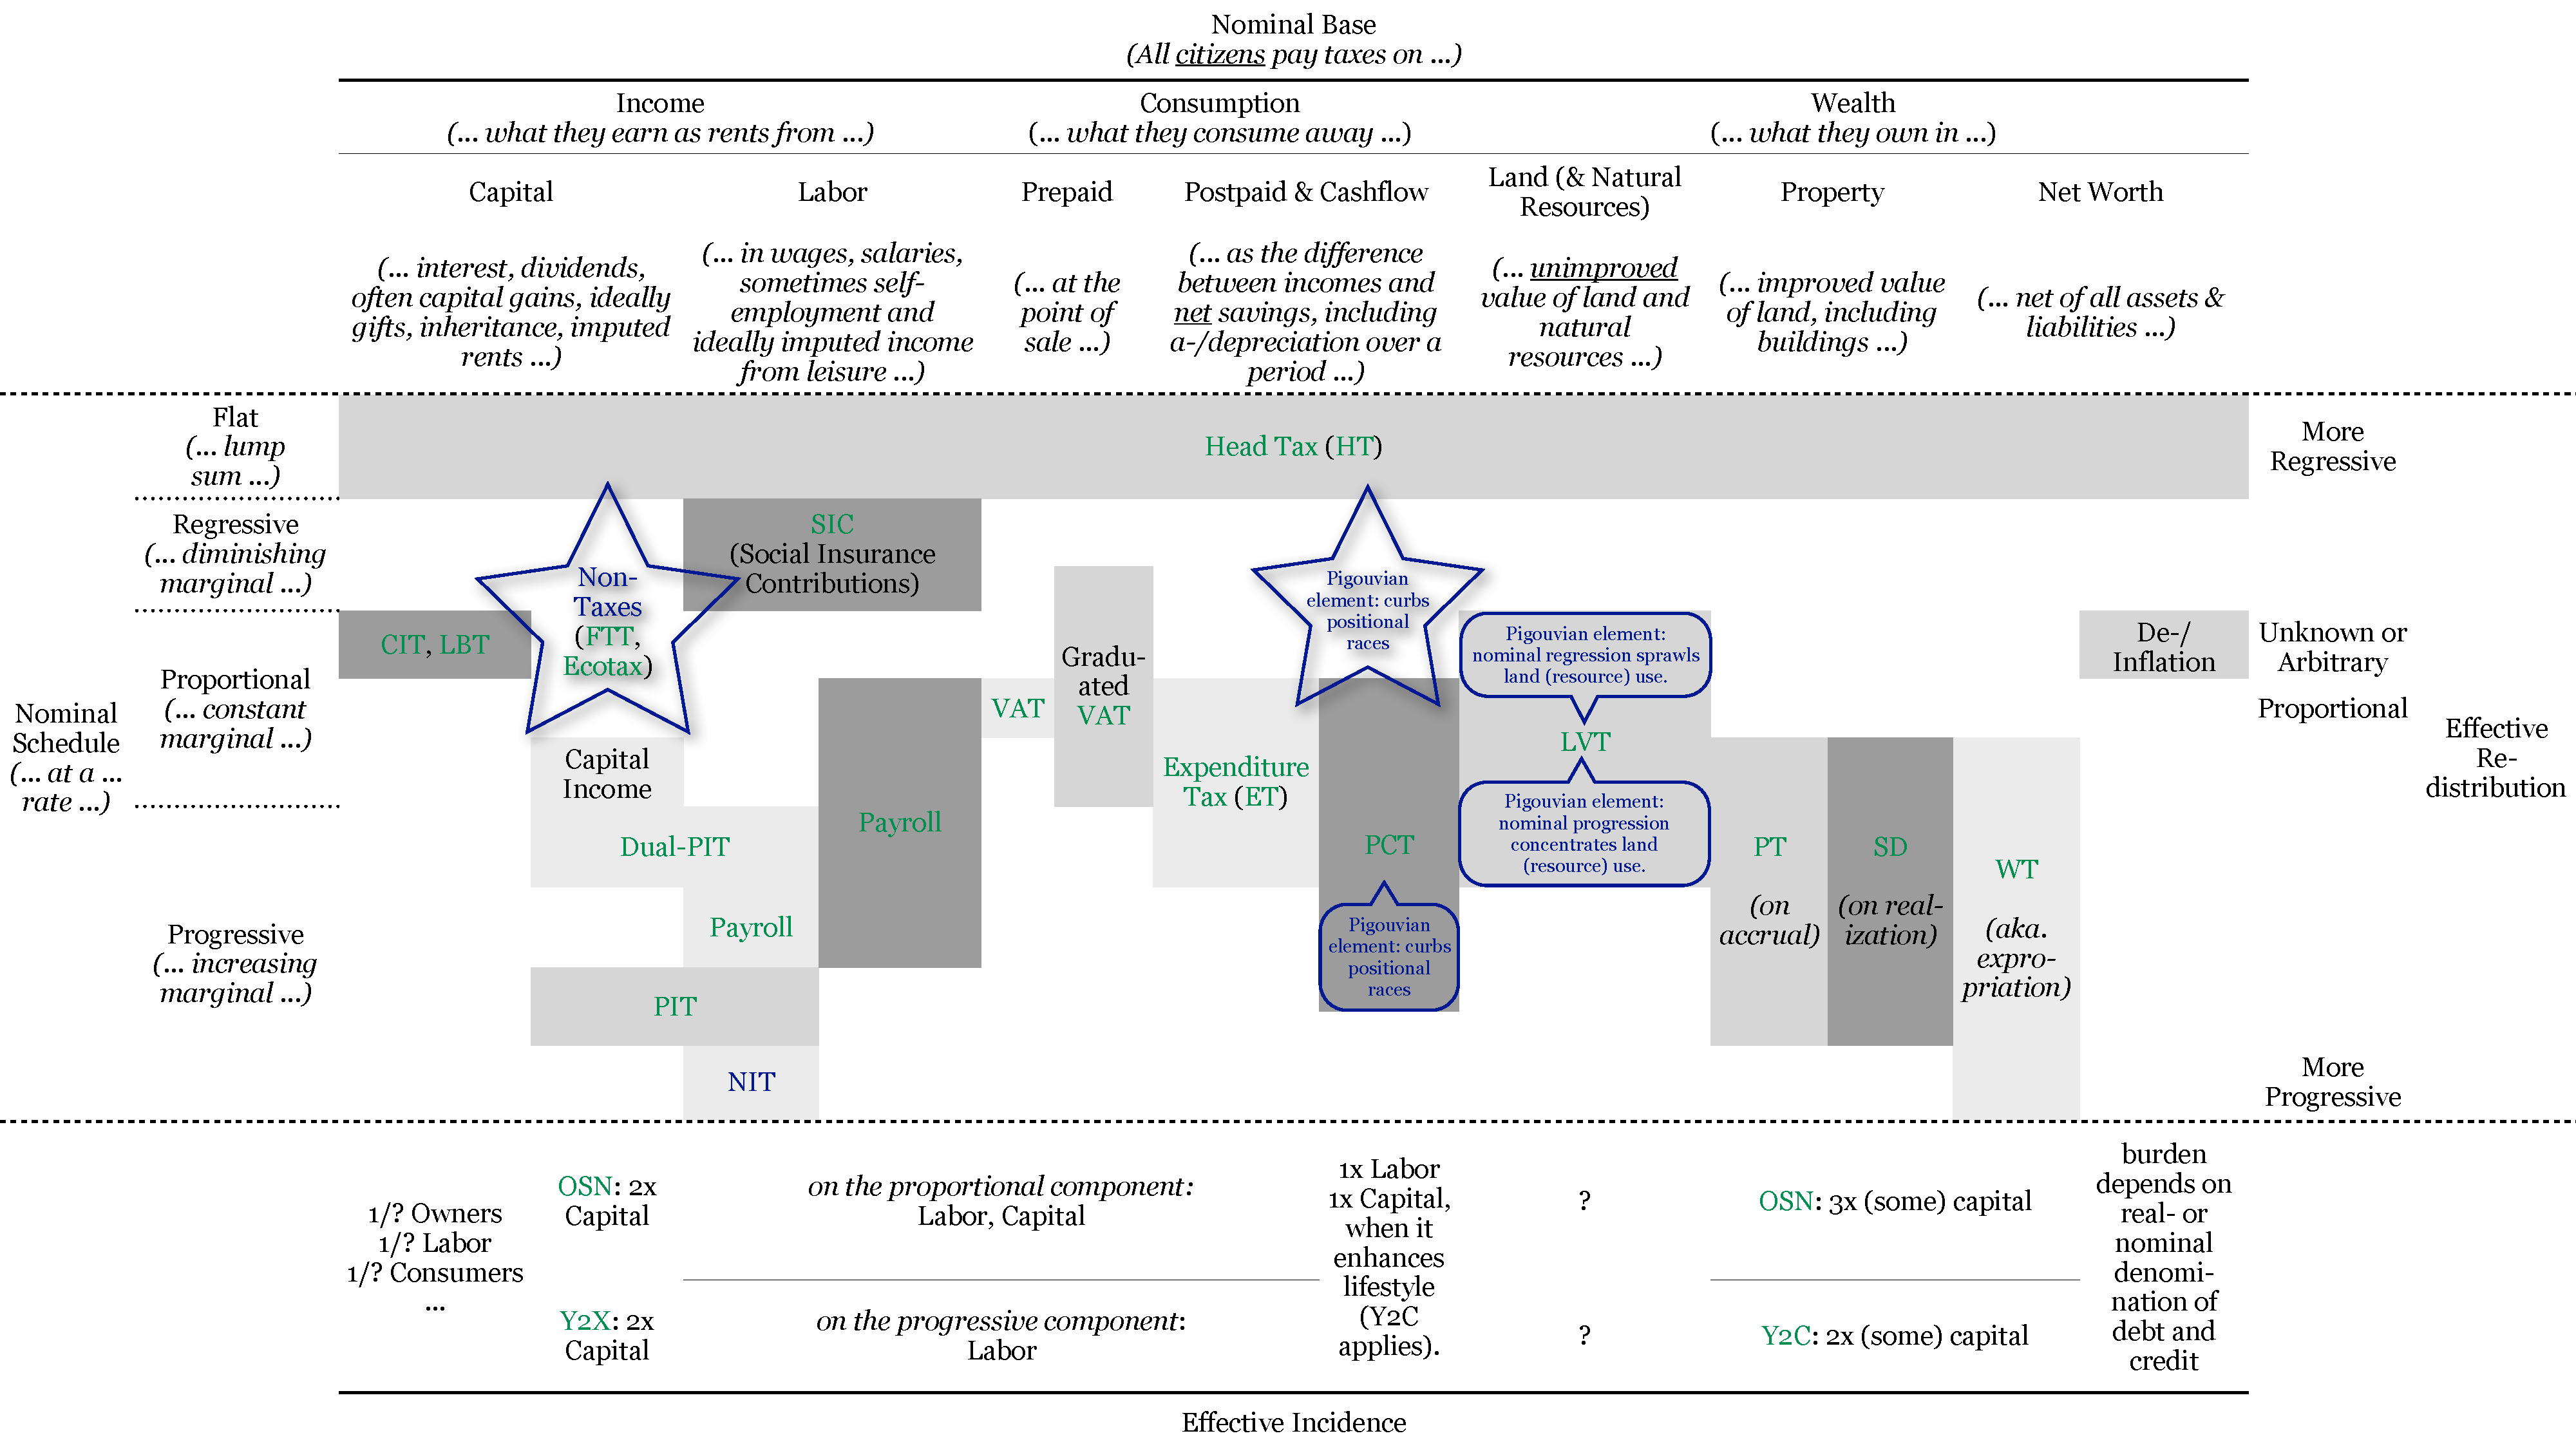
\includegraphics[width=1\textwidth]{tax-overview}
	\caption{Incidence and Redistribution of Modern Taxes}
	\label{tab:tax-overview}
	\end{center}
	%!TEX root=../tax-democracy-held.tex

\scriptsize{
	\glsfirst{CIT},
	\glsfirst{Dual-PIT},
	\glsfirst{Ecotax},
	\glsfirst{ET},
	\glsfirst{FTT},
	\glsfirst{LBT},
	\glsfirst{LVT},
	\glsfirst{NIT},
	\glsfirst{OSN},
	\glsfirst{PCT},
	\glsfirst{Payroll},
	\glsfirst{PT},
	\glsfirst{SD},
	\glsfirst{VAT},
	\glsfirst{WT},
	\glsfirst{Y2C} and

	\hyperref[sec:distributive-effects-of-inflation]{the distributive effects of in- and deflation} (p.~\pageref{sec:distributive-effects-of-inflation}).
}
\end{figure}
\end{landscape}
%this float seems too large

If their democratic rule is to be enlightened, deliberators must also engage a set of abstractions concerning its \hyperref[sec:tax-optimality]{optimality} (p.~\pageref{sec:tax-optimality}), \hyperref[sec:tax-justice]{justice} (p.~\pageref{sec:tax-justice}) and \hyperref[sec:tax-sustainability]{sustainability} (p.~\pageref{sec:tax-sustainability}) as well as problematize the view of human motivation, utility and rationality implied by these (economic) abstractions.
Deliberators must also understand the means and ends of an (ideal) mixed economy within which taxation reconciles allocation by plan and by exchange, including respective government and market failures.
\citeauthor[K1513]{Warren2008}, reporting on the \gls{ca}, notes that such learning phases are ``crucial to its ability to  render a decision, and indeed'' and that it \emph{can be done}:
``the decision was a learned and sophisticated one'';
``Most members transformed themselves from lay citizens with little knowledge of electoral systems into experts over a period of several months (\ldots)'' \citeyearpar[K1513]{Warren2008}.
Any deliberation that fails to engage such technical but broadly consensual --- if not entirely coherent --- concerns, must be considered unenlightened.
It would ignore some of the causal relationships and moral alternatives that we must assume exist, if and to the extent that we accept the economic \hyperref[sec:ontology]{ontology} (p.~\pageref{sec:ontology}) of \hyperref[chap:mixed-economy]{coexisting states and markets} (p.~\pageref{chap:mixed-economy}).

\paragraph{Deliberation}
Deliberation is no such catalogue of first-order considerations of what would make a good (efficient, fair, sustainable) decision in any given policy field, but instead, a second-order prescription to resolve disagreement \emph{over} those very the moral and causal arguments \citep[125]{GutmannThompson-2004-aa}.
Still, and in contrast to pluralism, it places more than just \emph{procedural} claims, but posits \emph{substantive} requirements for how agreement must be reached.
Succinctly, \citeauthor{GutmannThompson-2004-aa} demand that ``your fellow citizens must give reasons that are comprehensible to you'' \citeyearpar[K177]{GutmannThompson-2004-aa}.
More than merely intelligible, permissible arguments to reach deliberative agreement must raise validity \citep{Habermas-1984} and moral \citep{Rawls-1971} claims \emph{universally} acceptable to everyone.

Logically, it must then be theoretically possible for any \emph{given} argument to \emph{fail} that test, and to be impermissible --- including the arguments brought forward by experts.
In fact, deliberation reserves no special place for nominal experts at all, except if and to the extent that these experts have arrived at, and present their agreement under the standards of deliberation.
%\footnote{
%	As this PhD student can attest, there can be some doubt about whether (German social) science is really ruled by nothing but the ``unforced force of the better argument'' \cite[305]{Habermas1996}.
%}.

As noted in the above, any research design that axiomatizes any disagreement between experts (or ex-ante logic) as \emph{misunderstandings} on the part of the non-experts fails the deliberative standard, no matter the supposedly enlightening de-biasing treatments.

\paragraph{Reciprocity}
The desiderata of taxation and deliberation are seemingly in conflict.
Taxation requires people to consider an exogenously given catalogue of abstractions, and deliberation implies that no such set of arguments can be unconditionally accepted.
This is a general contradiction of procedural and substantively epistemic formulations of deliberative democracy \cite[402]{Bohman1998}.

This impasse has real repercussions for the proposed research design:
apparently, it can serve only one master.
Either, participants misunderstandings can be revealed by treating them with introductory economics, \emph{or} they can deliberate any which arguments they themselves find comprehensible.

As with so much that deliberative theory is up against
\footnote{
	For example, political participation versus enlightened understanding versus political equality, as \citeauthor{Fishkin2009} points out.
}, %correct this
this is a false dichotomy.

Argumentative reciprocity implies that expert knowledge be neither presumed, nor negated, but that these arguments --- as all others --- be allowed to demonstrate their universal causal and moral validity.

%``Mutual justification means not merely offering reasons to other people, or even offering reasons that they happen to accept [\ldots] \citep[98]{GutmannThompson-2004-aa}.
%	It means providing reasons that constitute a justification for imposing binding laws on them.
%	What reasons count as such a justification is inescapably a substantive question.
%	Merely formal standards for mutual justification --- such as a requirement that maxims implied by laws be generalizable --- are not sufficient.%plagiarism?

Expert- and non-expert (as all other) arguments must not merely be balanced in terms of airtime or affect, but ``the considerations offered in favor of, or against, a proposal, candidate or policy [must] be answered in substantive way by \emph{those who advocate a different position}'' \citep[K550, emphasis added]{Fishkin2009}.
Deliberation is, in other words, when non-experts answer expert arguments \emph{on their own, expert terms}, and vice versa, too.
Surely, the relation of this ideal to practice is ``aspirational'', too, as all in deliberation \citep[K2679]{Fishkin2009}.
So far, democratic theorists have failed to show ``how to incorporate the need for expertise and technical administration in a deliberative democracy'' \citep[515]{Thompson2008} and ``[a] great deal of work on deliberative theory focuses on conflicting values, religious toleration, identities and so on, and relatively little on conflicting facts'' \citep[2]{Moore2011}.

%\footnote{
% And maybe, in democracy, too, as William H.~Hastie (1904-1076), the first African American Justice on the U.S.\ Supreme Court warned us:
% \begin{quote}
% 	\emph{``Democracy is not being, it is becoming.It is easily lost, but never finally won''.}
% \end{quote}
%}.
Yet, for the deliberative experimenter, this aspiration to argumentative reciprocity is the ultimate hypothesis in need of  falsification, including reciprocity with expert arguments.
If expert knowledge on taxation is presumed valid, and any dissent chalked up as misunderstandings the aspiration of communicative action could \emph{never} be falsified.
Likewise, if expert knowledge on taxation is not given adequate opportunity to be reciprocally considered on its own terms, communicative action will \emph{always} be violated.
Neither of those formats would provide construct-valid deliberation.
Expert knowledge is then ``a special case of the general problem of convincing those who are not `in the room' to accept the results of a deliberation in which they did not directly participate'' \citep[2]{Moore2011}.
This problem can only be resolved by a ``democratic conception of expert authority'' \cite[2]{Moore2011}, that is, if deliberative standards are extended to expert arguments, too.
A good deliberative format brings ordinary citizens into this business:
they must be enabled to the farthest extent possible to argue expert as well as non-expert claims on their own terms, including the possibility to reject expert opinion if it is found insufficiently reciprocal in argument.

Because bringing ordinary citizens into this business, and \emph{equally} so, is, as \citeauthor{Rosenberg-2002-aa}'s so difficult, deliberations must ``be regarded as remedial institutions'' \citeyearpar[12]{Rosenberg-2007-aa} and more, ``they must be sites for political education and development'' \citeyearpar[13]{Rosenberg-2007-aa}.

\subsection{Format}
Consequently, a good format for deliberating tax includes a strong learning component, where participants are introduced to the structured choices and relevant abstractions suggested by experts, including their disagreements, conditions and uncertainties.
Deliberators are unlikely to cover these extensive grounds by themselves, or pick them up from (very limited) briefing books and will benefit from well-planned lessons.
On the other hand, a good format must also feature extensive small-group discussion, where participants talk amongst themselves, shielded from the authority of expertise.
Deliberators may benefit from a trained, non-expert moderator and/or scribe to assist, structure and document their discussion.
Most importantly, participants must be encouraged to adjudicate the validity claims of economics, to contrast and possibly relate those to their own, and other claims.

As noted earlier, most deliberative formats include --- often moderated --- small-group discussion, but few add to that a substantive learning component.
\footnote{
	\glspl{dp}, the pronounced methodological gold standard of deliberation \citep{Mansbridge2010} are too short to feature long lessons, and confine expert knowledge to ad-hoc question and answer sessions with experts and limited briefing books \citep{Fishkin2009}.
	Citizen Juries \citep{SmithWales-2000-aa}, Planning Cells \citep{Dienel-1999-aa} and related formats also include no learning components, and some experimenters even advise against expert knowledge.
	%add source
}
Among those that do are the small-n Danish-developed Consensus Conferences \citep{Grundahl1995} and especially the large-n, one-off \gls{ca} in British Columbia, Canada \citep{Citizen-2004-aa}.
Consensus Conferences have been held on very technical issues, including nanotechnology \citep{LeeKleinman2007} or genetically modified foods, and the Citizen Assembly was tasked to recommend an alternative electoral system for the province.
Much like taxation, technology policy, and especially electoral systems design also demand highly structured choices  (for example, a seat allocation rule or regulation) and raises a set of abstractions (party systems or risk distributions).

In a Consensus Conference, 12-15 self-selected but diverse citizens discuss a technical matter of political relevance for three or more days (!) and issue a report on their discussions \citep{LeeKleinman2007}.
In preparation for the conference, participants read quite extensive background material, which they discuss during the first of several daylong sessions.
At later sessions, they (publicly) share their questions with experts and finally draft a report for the sponsoring body and/or the media.
\citeauthor{LeeKleinman2007} report that a positive atmosphere, good organization and skillful facilitation are necessary for a successful Consensus Conference.
They also recommend that participants tell their stories, which moderators then weave into themes, to help citizens relate their experiences to expert knowledge \citeyearpar[159]{LeeKleinman2007}.

The \gls{ca} expanded on this model.
Over the course of a year, 160 randomly selected British Columbians read and learned about electoral systems, held public hearings, deliberated amongst themselves and, after several intermediate votes, recommended a (quite complicated) \gls{stv}-variant and drafted a report \citep{Citizen-2004-aa}.
The extensive learning phase, spanning six (!) weekends stands out among deliberative experiments.
In addition to a university-level textbook on electoral systems, Citizens received interactive lectures accompanied by small discussion groups.
An expert panel vetted the learning phase for impartiality and accuracy of information.
Participants also developed a set of shared values during the learning phase, both (procedurally) for how they wished to deliberate and (substantively) for a desirable electoral system.

\subsection{Implementation}
The \gls{ca} provides an ideal blueprint for a deliberative forum on tax;
however, limited resources and lack of experience do not permit such a large undertaking for this project.

Instead, the project proposed here is a scaled-down hybrid, combining the ambitious learning phases of a Citizen Assembly,
	%use gls instead
\footnote{
	The \gls{ca} also featured a ``listening phase'' \citep[1609]{Pearse2008} during which members held public hearings throughout the province, drawing some 3,000 attendees and 1,600 written submissions.
	Both because I do not have the resources and --- absent a mandate --- expect limited public interest, I plan no such phase.
}
with the more intimate, small-n interaction and participant empowerment of Consensus Conferences.

A small, self-selected sample of 15-24 diverse, ideally randomly-sampled, citizens will attend around 6 days of learning and deliberation spread over several weeks.A provisional schedule is included in \autoref{tab:schedule} (p.~\pageref{tab:schedule}).

%!TEX root=../tax-democracy-held.tex

\begin{landscape}
\footnotesize
%\begin{longtabu}[]{p{1cm}p{2.7cm}p{3cm}p{3cm}p{3cm}p{3cm}p{3cm}}
\begin{longtabu}[]{XX[2]X[2]X[2]X[2]X[2]X[2]X[2]}
\caption[Schedule]{Schedule for a Deliberative Forum on Tax\label{tab:schedule}}\\

\toprule

\emph{}
&\emph{Day 1}
&\emph{Day 2}
&\emph{Day 3}
&\emph{Day 4}
&\emph{Day 5}
&\emph{Day 6}
&\emph{Day 7}
\\

\midrule

09:00-10:30
&	Arrival
&	\cellcolor{darkgray}
	\nameref{chap:mixed-economy}:
	\nameref{sec:ends} (p.~\pageref{sec:ends})
&	\cellcolor{darkgray}
	\nameref{chap:mixed-economy}:
	\nameref{sec:trade-offs} %(p.~\pageref{sec:trade-offs}),
	\nameref{sec:smoke-n-mirrors}, % (p.~\pageref{sec:smoke-n-mirrors}),
	\nameref{sec:real-dissavings} %(p.~\pageref{sec:real-dissavings})
	(p.~\pageref{sec:trade-offs}ff.)
&	\cellcolor{darkgray}
	\nameref{chap:desirable-tax}:
	\nameref{sec:tax-optimality} (p.~\pageref{sec:tax-optimality})
& 	\cellcolor{darkgray}
	\nameref{chap:doable-tax}:
	\nameref{sec:tax-incidence} (p.~\pageref{sec:tax-incidence}),
	\nameref{sec:tax-elasticity} (p.~\pageref{sec:tax-elasticity})
&	\emph{--- Buffer ---}
&	\cellcolor{darkgray}
	\nameref{chap:better-tax} (p.~\pageref{chap:better-tax})
\\

Break
&
&
&
&
&
&
&
\\

11:00--12:00
& 	Introduction
&	\cellcolor{lightgray}
	Small Group: What do we want from market, state?
& 	\cellcolor{lightgray}
	Small Group: What alternatives does a mixed economy face?
& 	\cellcolor{lightgray}
	Small Group: What makes a tax efficient?
&	\cellcolor{lightgray}
	Small Group: Who really pays a tax, and why?
&	\cellcolor{lightgray}
	Small Group: What do we want to know from experts?
&	\cellcolor{lightgray}
	Small Group: What tax do we want?
\\



Lunch
&
&
&
&
&
&
&
\\

14:00-15:30
&	\cellcolor{lightgray}
	Small Group: Experiences, Questions, Stories on/with Tax
&	\cellcolor{darkgray}
	\nameref{chap:mixed-economy}:
	\nameref{sec:means} (p.~\pageref{sec:means})
&	\cellcolor{lightgray}
	Plenary: How should state and market co-exist?
&	\cellcolor{darkgray}
	\nameref{chap:desirable-tax}:
	\nameref{sec:tax-justice} (p.~\pageref{sec:tax-justice})
&	\cellcolor{darkgray}
	\nameref{chap:doable-tax}:
	\nameref{sec:tax-schedule}, %(p.~\pageref{sec:tax-schedule})
	\nameref{sec:tax-timing}, %(p.~\pageref{sec:tax-timing})
	\nameref{sec:tax-neutrality} %(p.~\pageref{sec:tax-neutrality})
	(p.~\pageref{sec:tax-schedule}ff.)
&	\cellcolor{lightgray}
	Expert Panel: Questions and Answers
&	\cellcolor{lightgray}
	Plenary: What tax do we want?
\\

Break
&
&
&
&
&
&
&
\\

16:00-17:30
&	\cellcolor{lightgray}
	Plenary: Distilling Guiding Questions, Criteria
&	\cellcolor{lightgray}
	Small Group: How can states and markets interface?
&	\cellcolor{darkgray}
	Overview of existing taxes
&	\cellcolor{lightgray}
	Small Group: What makes a tax just?
&	\cellcolor{lightgray}
	Small Group: At what rate, on what source, and when we tax?
&	\cellcolor{lightgray}
	Plenary: What did we learn from the experts?
&	\cellcolor{lightgray}
	Plenary: Write-up of Report
\\

%Dinner
%&
%&
%&
%&
%&
%&
%& Farewell Dinner
%\\

%20:00ff
%& Movie: 12 Angry Men
%&
%& Games Night
%&
%&
%&
%& Departure
%\\

\bottomrule
\end{longtabu}
\scriptsize{
	Light grey cells are \emph{deliberation phases}; participants discuss with one another in small group and plenary sessions.
	Their work is facilitated by a moderator and they a scribe.
	Dark grey cells are \emph{learning phases}; citizens participate in an interactive seminar held by the instructor.
	The seminar responds to the guiding questions identified by the participants.
	}

\end{landscape}

%\cite[K2485]{Pearse2008} speak of an ``epistemological deficiency, by failing to incorporate insights supplied by different group perspectives.''

After introducing the format and framing the issue, deliberators are invited to tell stories about experiences with taxation, following \citeauthor[67]{Mansbridge2010a}'s recommendation:
`Stories can establish credibility, create empathy, and trigger a sense of injustice, all of which contribute directly or indirectly to justification'' \citeyearpar[67]{Mansbridge2010a}.
Deliberators also share opinions and grievances about tax as well as identify relevant questions and issues, which will be taken up in, and structure the later learning phases.
During these learning sessions, taking up less than half of the time, participants receive information about the structured choices and relevant abstractions of taxation from the author.
These lessons are organized around themes and values identified by deliberators in an initial session, and attempt to relate the subject matter to participant experiences.
Learning sessions alternate with extensive small-group deliberations, during which participants reflect on the lessons, relate or contrast it to their own experiences and claims and adjudicate the validity of the presented moral and causal arguments.
Small-group deliberations are facilitated by a trained moderator, who has no expertise in taxation or economics.
At the end of the process, participants must agree on a tax and write a report outlining their recommendation, which can be released to the public.
If resources permit, participants will also hear a panel of expert witnesses to discuss their questions.

%The forum will be run twice, for two extreme case samples: once as an undergraduate class at the University of Bremen, and once as an adult evening class with the Volkshochschule and/or in association with organized labor.
%Participants in the university class will be graded, but not based on their contributions to the deliberations, to which the author and instructor will not be a party.
%The class will be advertised through the usual channels at the university.
%Participation in the adult evening class will be free of charge, deliberators may be reimbursed for local travel, receive free food and will be offered childcare.
%The class will be advertised through local organized labor to attract non-academic participants.

%a good format for my goal includes
    %Includes a strong learning component, structured roughly along my drafts -- but shorter, and in more accessible style.
%(It must not be a microeconomics text).
    %Relates these abstractions to personal experiences and intersubjective value judgments.
    %Prioritizes intensity (duration) over representativeness (sample size) under given constraints (time, money).
    %May involve me and existing material for the learning component, but someone else must moderate the deliberations.
    %Starts from a small-scale, face-to-face deliberation as a pilot study, both to guarantee concept validity and because I have no idea about deliberation-

    %Instead the same quasi-experimental design could be run with qualitative data, including, open-ended questionnaires and/or semi-structured interviews, or even a record of the deliberations.
%Such data could be content-analysed (or rather: coded) to distill the (mis)understanding before and after the treatment.

%note reciprocity, sharing ones causal assumptions

%note that the link between rosenbergs sequence thinking and my tax misunderstandings is still to be developed

%\cite{Azmanova2010} (also \cite{Fishkin2009}: 529)
	%49: thoughtfulness and reflexivity (as per Fishkin) require 1) reasonably accurate information 2) substantive balance 3) diversity, 4) conscientiousness, 5) equal consideration

%\cite{Citizen-2004-aa}
	%11: one guy did the learning sessions
	%1) has a selection phase
	%2)  has a LEARNING phase
		%also develop "shared values" about the process
	%3) has a PUBLIC HEARING phase
	%4) has a DELIBERATION phase
	%go to chrch with group, maybe.

%\cite{Fung-2003-ac}
	%very good summary, get back to this

%\cite{Fishkin2009}
	%democracies are supposed to fulfill two values; political equality and deliberation (loc.
%84)
	%``a democracy in which we all had substantive information [and] [\ldots] substantive opinions would seem to take too many meetings.''
	%what's wrong with unenlightened opinions (all loc.
%113ff)
		%\begin{enumerate}
			%\item they may be volatile (cite other sources
			%\item people may be manipulated by foregrounding some information (clean coal vs.\ dirty coal, forgetting about natural gas -- compare this to tax choice)
			%\item misinformation (savings rate)
			%\item favor favorable, true arguments over others
			%\item manipulation may ``prime'' one aspect of policy.
		%\end{enumerate}
	%K260: ``the hard choice, in other words, is between debilitated but actual opinion, on the one hand, and deliberative but counterfactual opinion, on the other.''
	%K369: table with raw/refined opinion, and different kinds of sampling.
	%K438: ``The idea is that if a counterfactual situation is morally relevant, why not do a serious social science experiment -- rather than merely engage in informal inference or armchair empiricism -- to determine what the appropriate counterfactual situation might look like?
%and if that counterfactual is both discoverable and normatively relevent, why not then let the rest of the world know about it?
%Just as John Rawls's original position can be thought of having a kind of recommending force, the counterfactual representation of public opinion identified by the \gls{dp} also recommends to the rest of the population some conclusions that they ought to take seriously.''
	%K390: self-selected samples will be very limited in what they can achieve.
	%K401: citizen juries use quota samples, consensus conferences use self-selected samples, then with some quota sampling
	%K550: notes that positions must not merely be balanced in terms of airtime or affect, but ``whether the considerations offered in favor of, or against, a proposal, candidate or policy are answered in a substantive way by those who advocate a different position.'' %THIS IS KEY!
	%K561: three categories for such considerations
		%``the benefits or burdens of a policy or political choice,
		% the causal arguments about whether those benefits or benefits or burdens will actually result from one choice or another,
		%and the values by which those benefits and burdens might best be evaluated.''
		%K1424: ``the problem is that any microcosmis deliberation taking place in a modern society will be one in which there are significant social and economic inequalities in the conduct of ordinary life in the broader society.
		 	%It seems difficult or impossible to `bracket' these inequalities -- for participants to behave `as if' they do not exist.
		 	%Indeed the problem goes deeper.
%The possibility of doing so is the challenge of the ``autonomy of the political'', namely, whether or not equality can hold sway in politics in a world in which inequality rules in economic and social relations.
		 	%The viability and legitimacy of the liberal-democratic process may turn on the answer.'' \citep[loc.
%2679]{Fishkin2009}

%\cite{GutmannThompson-2004-aa}
	%loc177: `your fellow citizens must give reasons that are comprehensible to you''
	%K188: they introduce first and second-order theories, too!
	%K919, writing about Fish: ``Giving reasons is the chief way of academics to exercise power in democratic politics.
%All the talk about deliberation, like deliberation itself, is merely a cover for power politics.''.

%iris marion young, especially notes that people of lower status may have a hard time getting listened to, or that others may be particularly accustomed to orderly forms of reason-giving arguments that weigh with other participants -- and this may be particulary problematic the more substantive the topic is.

%note that

%groupthink!

%tax allows only very limited choice: income, consumption or assets; a couple of schedules, plus some pigouvian taxation.
% the CIT, notably, is just a special way to raise the PIT.
%Otherwise, only natural persons.
%Tax demands these choices.
%Also, these choices \emph{are} as I explain in the below, political, so they must be made legitimately, and we may not be able to simply outsource them to elites.

%there remain problems: you can't just go about this as if it wwere not controversial; it is controversially maongst experts, but more importantly, controversial whether experts have in fact authority and the right context.
%It can't just be an experiment, or a treatment intervention where ordinary citizens must necessarily become more like experts, and if they are not, then the teaching has failed.
%It must be possible for people to disagree with the abstractions they ar epresented with, see the criticism of it.

%tax is very technocratic, simply because the instition is like that.
%this will have to be qualitative

%\gls{oecd}-world (\autoref{chap:3-crises}

%Tax offers/demands very structured choices: there are essentially only 4x3 broad tax types (see tax table in drafts).
%Different from, for example, a deliberation on “racial tensions”, deliberating tax choice is more close-ended.
%Tax expertise is easily politicized, because:
%Tax cannot be reduced to an empirical question, both because inframarginal data is not available, and because macroeconomics is incompletely understood.
%Tax cannot be reduced to a consequentialist inquiry, because people (may) care about other normative claims, too (for example, fairness).

%Tax cannot be easily (if at all) dumbed down to subsets of tax choice (for example, VAT vs PIT), or subsets of abstractions (for example, only “bastard keynesianism”) for two reasons:
    %Any such reduction would violate the spirit of deliberation; citizens could not set their own agenda.
    %Any such reduction may well fail to elucidate my hypothesized misunderstandings: I imagine “understanding tax” as a bucket, which, if leaky will drain to the lowest level.
%For example, if deliberators would discuss most aspects of taxation, but skip over the limits (!) of price controls, they may well opt for price controls in lieu of, or in addition to taxation

\section{Research Design}
%see below
%cases, people, selection
%methods of observation and/or inference

\subsection{Hypotheses}
The threefold research question raises several hypotheses:


\begin{figure}[htbp]
    \centering
	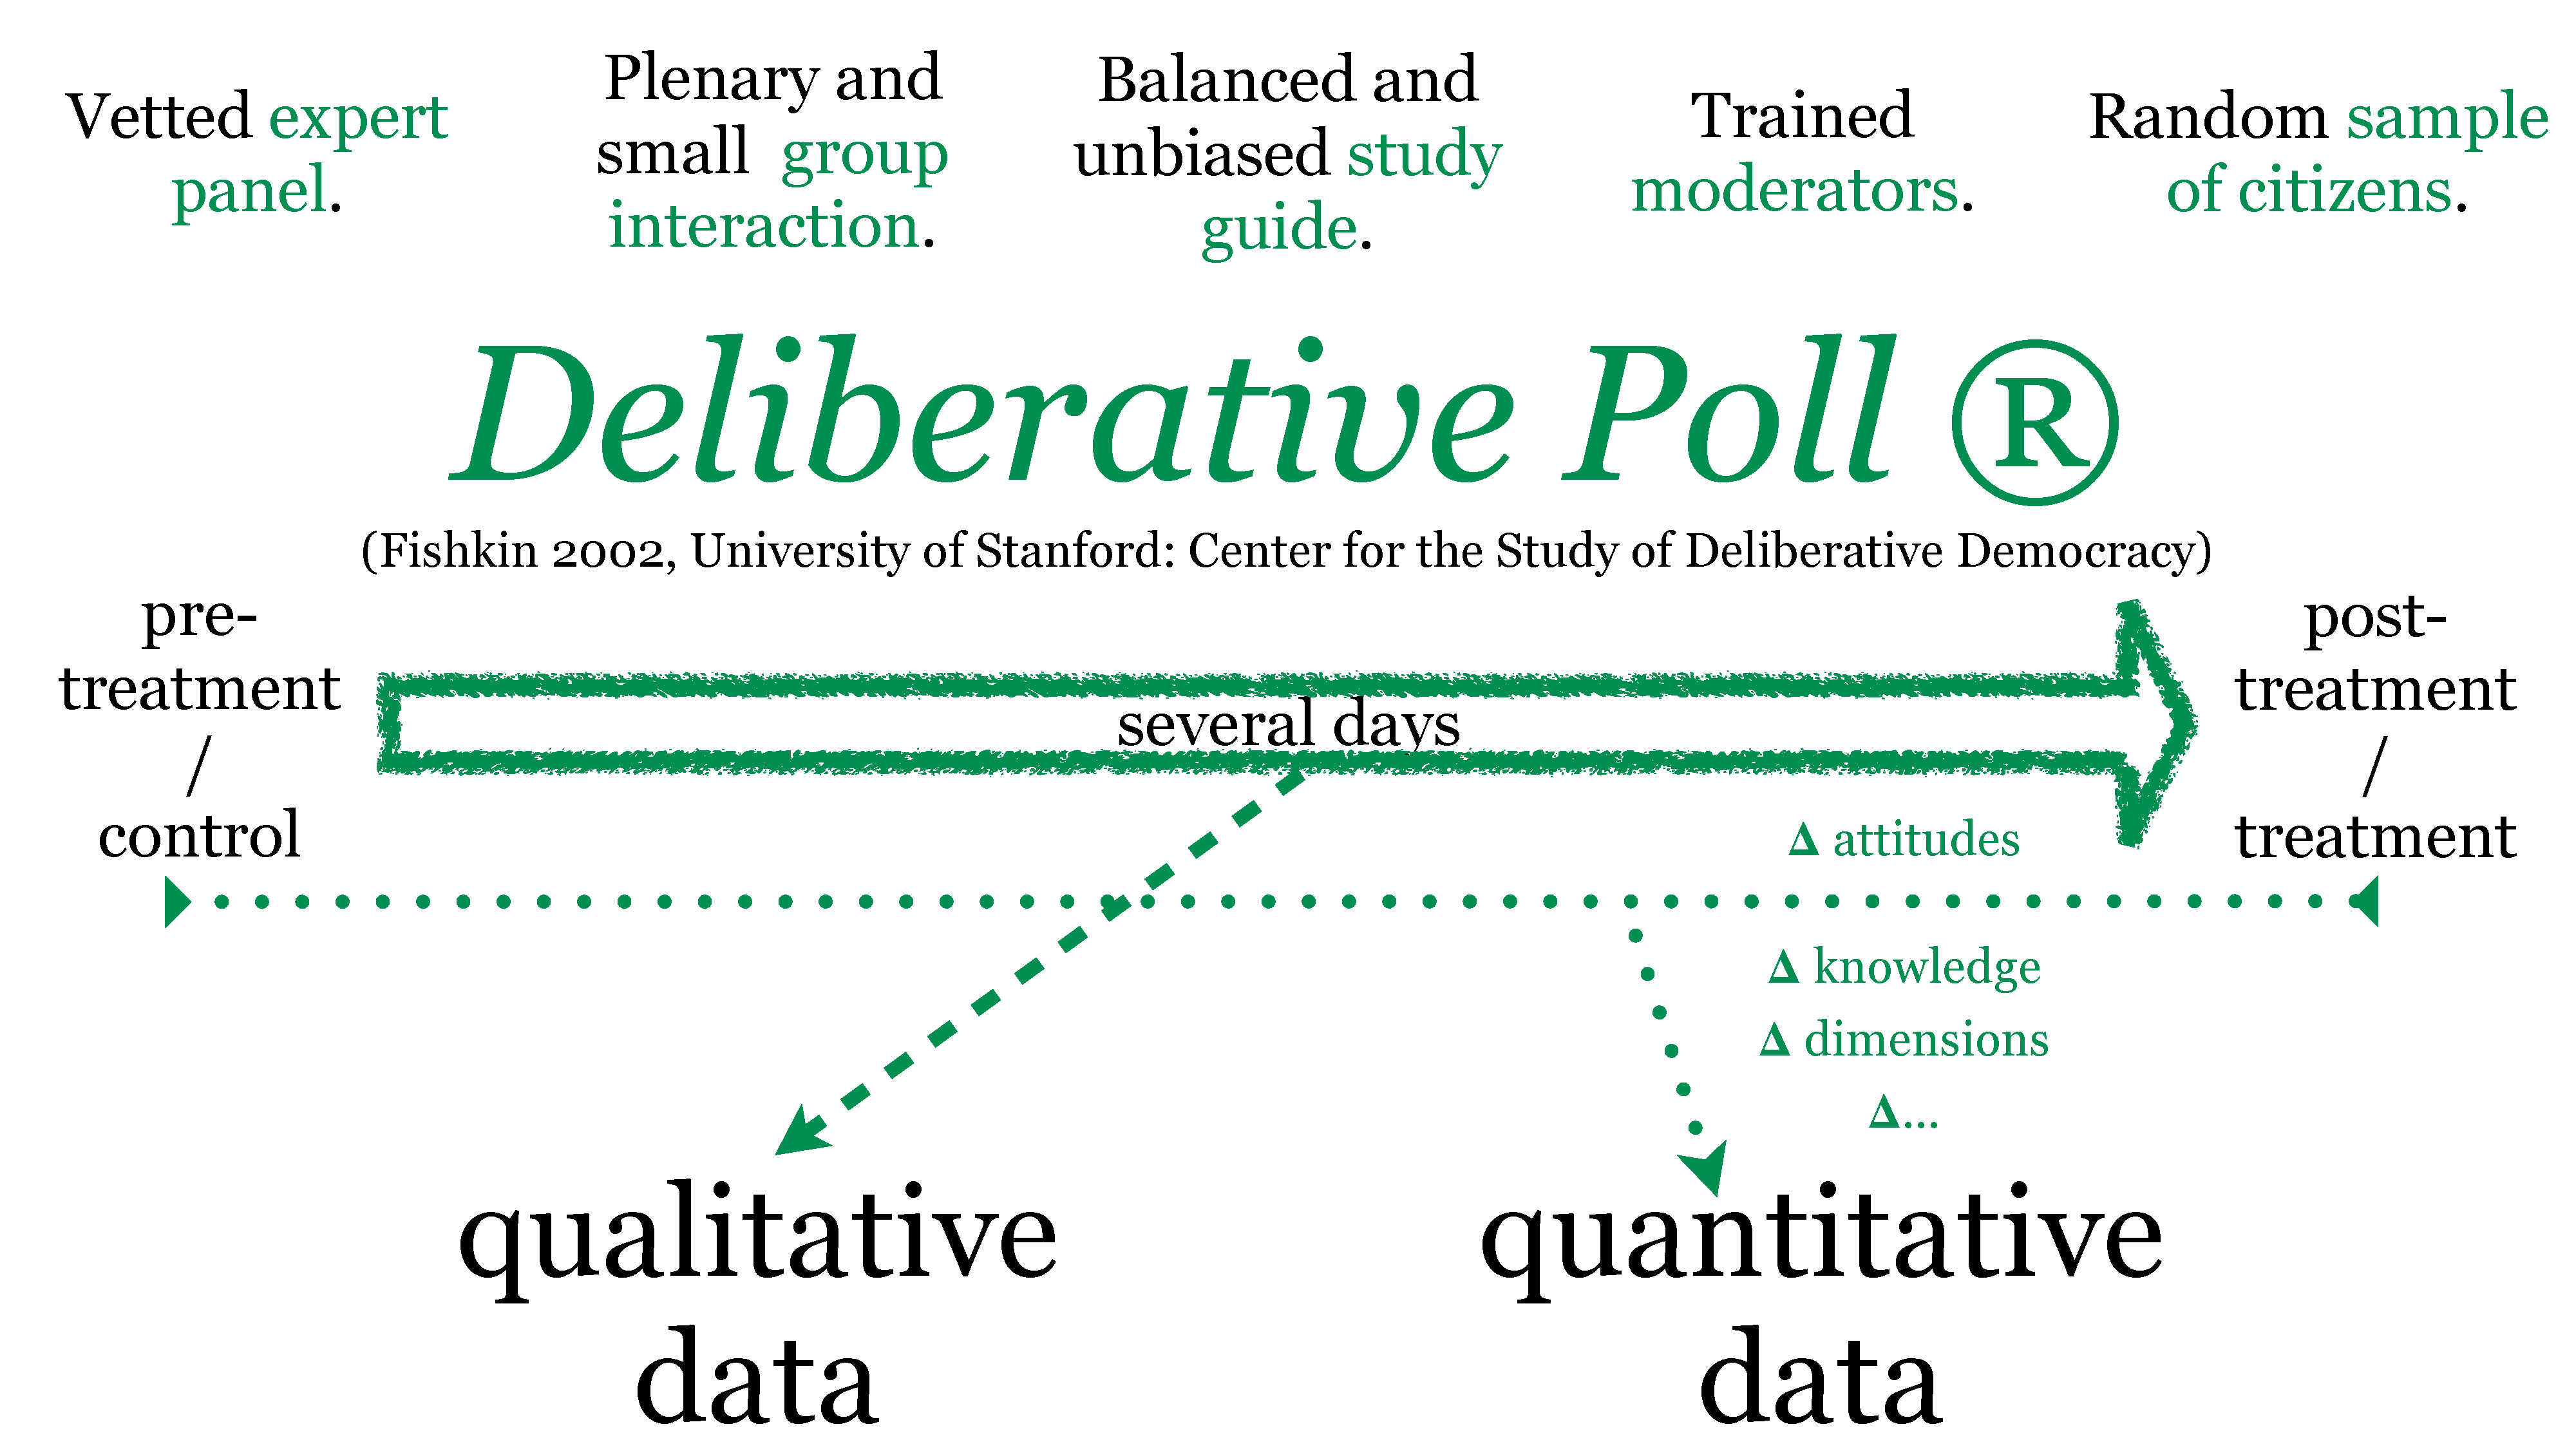
\includegraphics[width=1\linewidth]{deliberative-poll-method}
	\caption{Method of the Deliberative Poll}
	\label{fig:deliberative-poll-method(short)}
\end{figure}

\subsection{Quantitative Data}

Both research questions, about 1) the remaining disagreements about tax and 2) the ability of deliberative democracy to cover abstract and structured issues can be rolled up into one set of hypotheses.

\citeauthor{Fishkin2009} suggests that deliberation increases knowledge, and changes preferences as a function of such knowledge gain.
Similarly, I hypothesize that people will gain in knowledge about taxation, including resolving some systematic misunderstandings of concepts and causal relationships, some variants of which are already documented \citep{McCafferyBaron2003,Caplan2007}.
I furthermore hypothesize that \emph{as a function} of these knowledge gains, people will change their preferences on the desired base and schedule of taxation.
Additionally, deliberation will increase self-assessed autonomy and competence of participants, and they will find the presented alternatives of base and schedule more meaningful.
Learning interventions will further drive knowledge gain and improve self-assessments, but --- if it is sufficiently balanced --- \emph{will not} interact with attitude change.
%Both research questions \ref{itm:resolve-better-tax} and \ref{itm:prove-deliberative-democracy} can be rolled up in one set of hypotheses:

\begin{enumerate}
    \item \label{itm:think-different}
	If ordinary citizens are given the possibility to deliberate welfare and taxation, they will think differently about it.
	Specifically,

	\begin{enumerate}
		\item \label{itm:knowledge-gain} \emph{Knowledge Gain.}
		People will gain in knowledge.
		Specifically relevant for tax choice,
		%(\autoref{fig:tax-with-misunderstandings}, p.~\pageref{fig:tax-with-misunderstandings}), %requires that table to be in here

		\begin{enumerate}
			\item \label{itm:bastard-keynesianism} \emph{Bastard Keynesianism.}
			People will understand that an economy can have an arbitrary (sub-\citeauthor{Solow1956}) savings rate, and that --- equivalently --- if lowered slowly, aggregate \emph{consumption} will not depress aggregate \emph{demand}.

			\item \label{itm:real-myopia} \emph{Real Myopia.}
			%aka technocratic myopia
			People will understand that the future prosperity of an economy is, in part, determined by present \emph{net} investment, and that --- equivalently --- \emph{real}, not \emph{nominal} (for example, \gls{gdp}) indicators track the savings rate of an economy.

			\item \label{itm:bastard-hayekianism} \emph{Bastard Hayekianism.}
			%aka government vs markets
			%make naming consistent
			People will understand that an economy can adopt an arbitrary government quota (if, possibly, at a cost), and that --- equivalently --- not \emph{all} (but some) taxed resources are lost.
			Taxation is not exclusively or unconditionally a negative-sum proposition.

			\item \label{itm:flyper-theory} \emph{Flypaper Theory.}
			 %aka tax-aversion
			People will understand that ontologically and empirically, only and always \emph{natural} persons bear the burdens of taxation, and that --- equivalently --- the flypaper theory of tax incidence is false.

			This hypothesis is similar to, but not identical to \citeauthor{McCafferyBaron2003}'s findings of \emph{tax aversion}, by which people mistakenly prefer taxes not labeled as such and/or indirect taxes and a \emph{disaggregation effect}, by which people fail to integrate taxes on same bases.
			%might have to feature tax aversion separately, because that is already in the visualizatiuon

			\item \label{itm:ordoliberal-mess} \emph{Ordoliberal Mess.}
			%not hygiene, that's the opposite
			People will understand that Pigouvian and general-revenue taxes follow opposing logics, and that --- equivalently --- a Pigouvian tax \emph{should not} raise revenue.

			This hypothesis is similar to, but not identical to \citeauthor{McCafferyBaron2003}'s findings of a \emph{disaggregation effect}, by which people fail to integrate different taxes even on same bases.%this is (\cite{McCaffery2003}: 19ff)
			%is this really right?

			\item \label{itm:false-omnipotence} \emph{False Omnipotence.}
			%clarify labeling
			%used to be negative some
			People will understand that taxation will often (if not always) cause unintended consequences in markets, or that --- equivalently --- taxation can cause a negative-sum \glspl{dwl}.
			Taxation is not exclusively or unconditionally a zero-sum proposition.

			\item \label{itm:false-omniscience} \emph{False Omniscience.}
			Relatedly, people will understand that taxable income and wealth (but not consumption) cannot be measured independent of market-pricing, or that --- equivalently --- any taxation based on fiat evaluations may have unintended consequences in markets.
		\end{enumerate}

		\item \label{itm:universal-validity} \emph{Universal Validity}
		People will find the above abstractions meaningful and accept a universal validity of underlying causal and moral arguments.
%			\item \label{itm:preference-structuration}
%				\emph{Preference structuration.}
%				Partly as a function of the above knowledge gain, people will have better-structured preferences over taxation.

%				Specifically, and related to the cyclical preferences \citep[334]{Farrar2010} and other aggregation failures of pluralist democracy \citep[for example,][]{Condorcet1785,Arrow1963},

%				\begin{enumerate}

%					\item \label{itm:vNM-consistent}
%						\emph{\glsfirst{vnm}-Consistency.}
%						\emph{Individually}, people will have ordinal preferences that more closely resemble \gls{vnm}-consistency.

%					\item \label{itm:single-peakedness}
%						\emph{Single Peakedness.}
%						\emph{In the aggregate}, people will have preferences that more closely resemble single-peakedness.

%					\item \label{itm:orthogonal-dimensions}
%						\emph{Orthogonal Dimensions.}
%						\emph{In the aggregate}, people will have preferences that more closely resemble orthogonal factors.
%				\end{enumerate}

		\item \label{itm:attitude-change} \emph{Attitude Change.}
		Partly as a function of the above effects %(as in \autoref{fig:tax-with-misunderstandings}, p.~\pageref{fig:tax-with-misunderstandings}), %not working
		people will prefer a \glsfirst{pct}, conditionally supplemented by a \glsfirst{wt}, \glsfirst{lvt} and \glsfirst{nit} over the present tax regimes of \glsfirst{pit}, \glsfirst{vat} and \glsfirst{payroll}.
	\end{enumerate}

	\item \label{itm:meta-assessment} \emph{Meta Assessment}

	\begin{enumerate}
		\item \label{itm:autonomy} \emph{Autonomy.}
		People will consider themselves more effectively autonomous in discussing and choosing basic tax regimes.

		\item \label{itm:competence} \emph{Competence.}
		People will consider themselves more competent in discussing and choosing basic tax regimes.

		\item \label{itm:meaningful-choice} \emph{Meaningful Choice.}
		People will find the choices of tax base and schedule to be more meaningful to express their political autonomy.
	\end{enumerate}

	\item \label{itm:learning-interventions} \emph{Learning Interventions.}
	A learning interaction targeted at one of the above-listed knowledge gains will further that knowledge gain.

	\item \label{itm:interaction-effects} \emph{Interaction Effects.}
	The above effects will:

	\begin{enumerate}
		\item \label{itm:interact-equity}
		\emph{Not interact} with people's equity beliefs, or --- equivalently --- people will not change their thinking about tax as a function of their allocative preferences.

		\item \label{itm:interact-ses}
		\emph{Interact negatively} with people's socio-economic status, or --- equivalently --- people with greater socio-economic status will change their thinking about tax the least.
%				\item \label{itm:interact-cognitive-ability}
%					\emph{Interact negatively} with people's cognitive ability, or --- equivalently --- people with less cognitive ability will change their thinking about tax the least.
		\item \label{itm:interventions}
		\emph{Intervention-interaction}
		\begin{enumerate}
			\item Of the above effects, meta assessments will \emph{interact positively} with learning interventions.
			\item Of the above effects, attitude changes will \emph{not interact} with learning interventions over and above the effect mediated by knowledge gain.
		\end{enumerate}
	\end{enumerate}
\end{enumerate}

%\begin{landscape}
% \begin{figure}[htbp]
%    \begin{center}
%	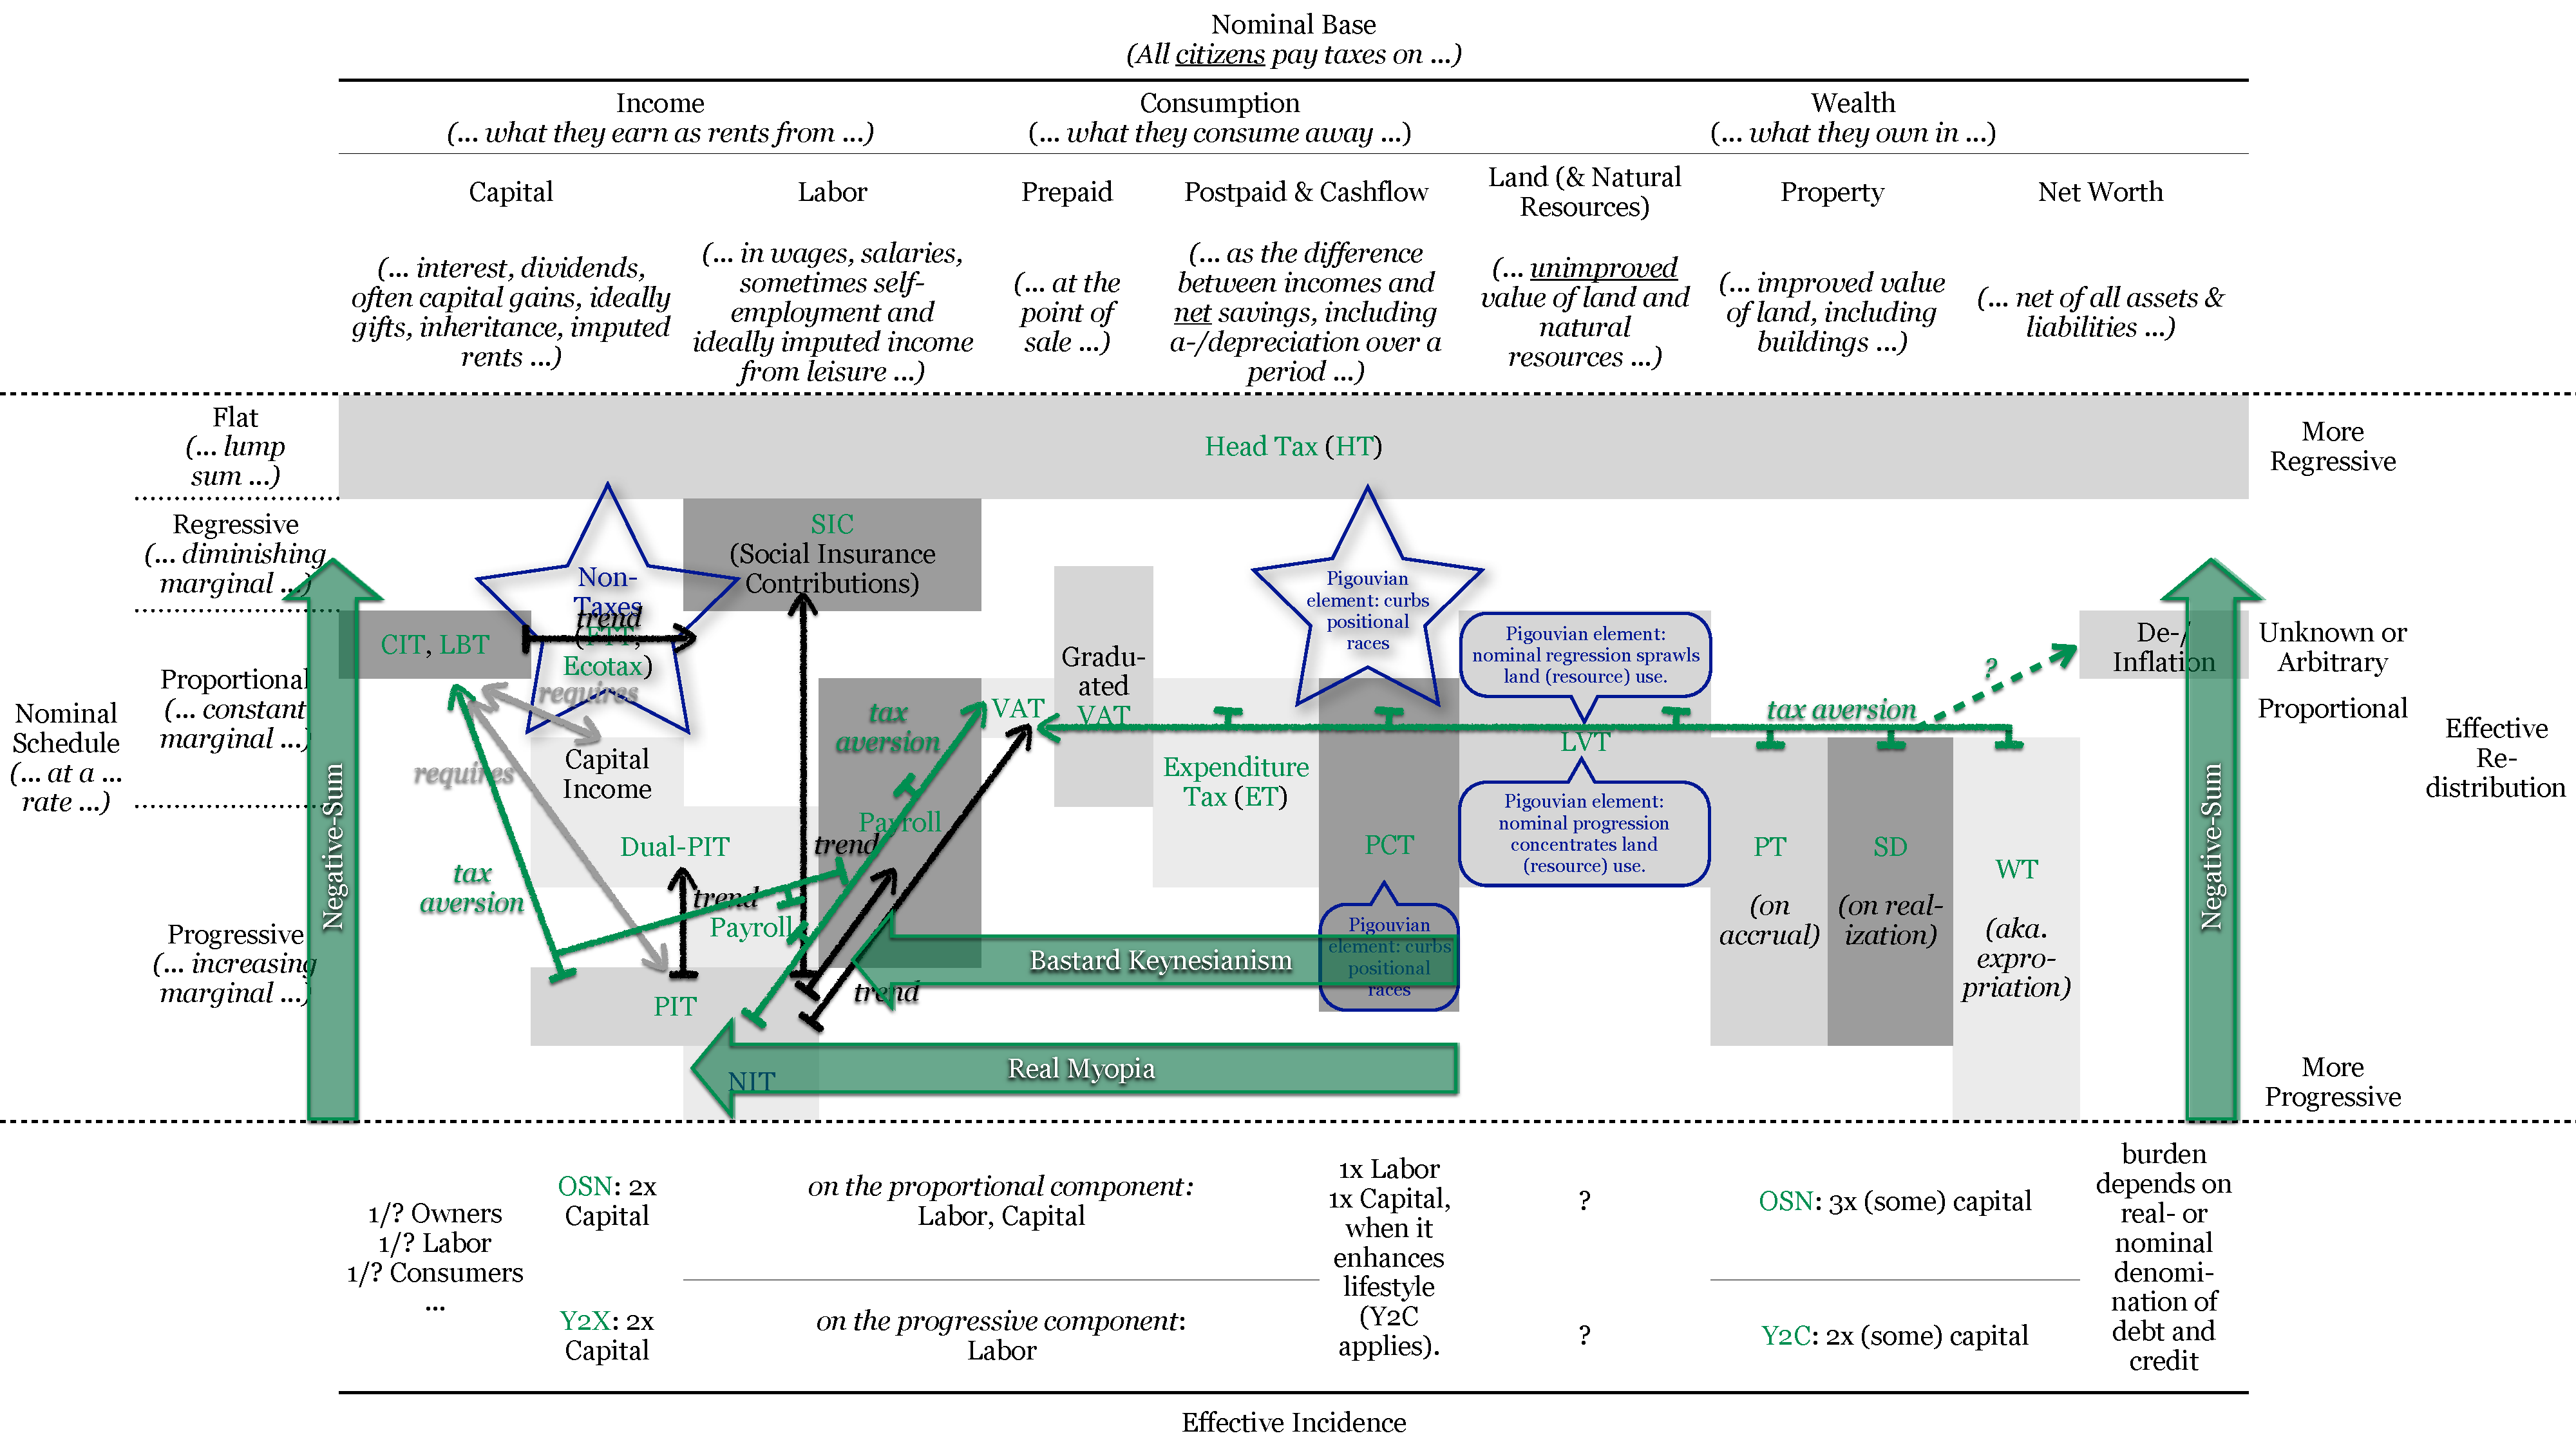
\includegraphics[width=1\linewidth]{tax-with-misunderstandings}
%	\caption[The Vector Field of Taxes with Misunderstandings]{The Vector Field of Taxes with Misunderstandings}
%	\label{fig:tax-with-misunderstandings}
%	\end{center}
%%	%!TEX root=../tax-democracy-held.tex

\scriptsize{
	\glsfirst{CIT},
	\glsfirst{Dual-PIT},
	\glsfirst{Ecotax},
	\glsfirst{ET},
	\glsfirst{FTT},
	\glsfirst{LBT},
	\glsfirst{LVT},
	\glsfirst{NIT},
	\glsfirst{OSN},
	\glsfirst{PCT},
	\glsfirst{Payroll},
	\glsfirst{PT},
	\glsfirst{SD},
	\glsfirst{VAT},
	\glsfirst{WT},
	\glsfirst{Y2C} and

	\hyperref[sec:distributive-effects-of-inflation]{the distributive effects of in- and deflation} (p.~\pageref{sec:distributive-effects-of-inflation}).
}
%\end{figure}
%\end{landscape}

\subsection{Data and Methods}
To clearly measure the hypothesized $\Delta$ in knowledge and preferences, but also to verify argumentative reciprocity and to directly observe (or problematize) communicative action, this project will utilize both survey and process data.

Akin to the \gls{dp}s, participants will be asked to respond to closed- and open-ended survey questions on tax issues, both before and after the forum.
The surveys will also gather basic socio-economic data and invite feedback on the deliberative forum itself.
This data can be compared before and after the deliberative treatment within-subjects.
Lacking a sufficiently large sample, in lieu of quantitative analysis of closed-ended questions, responses to open-ended questions will be qualitatively coded and compared with the hypothesized (mis)understandings.

Additionally, process data from the deliberation will be gathered, comprising of the claims, themes and questions raised by participants and summarized by the moderator and/or scribe at the end of each deliberation, as well as the final report on taxation and other documents or notes produced during the deliberation.
Deliberations will also be audio-(visually) recorded, although comprehensive transcription and analysis of this data will probably not be possible.
This process data and select recordings will then be subjected to a qualitative content analysis, both to verify that participants \emph{could} make arguments reciprocally comprehensible (and otherwise valid), and to record which of several arguments deliberators accepted as based on universal validity claims.

\section{Feasibility}
This project is theoretically, methodologically and organizationally demanding, but it can be completed in about 2 years.
In my prior work on the mixed economy and taxation, I have already distilled a compact set of abstractions and choices to be considered by deliberators.
Existing chapters (\ref{chap:wanted}--\ref{chap:better-tax}, p.~\pageref{chap:wanted}ff.) provide a good basis for the briefing material, learning phases, questionnaire development and qualitative analyses.
Happily, these chapters abstract away much of the political controversy over economic issues, clearly state remaining expert dissent and, rather than definitive answers, present a catalogue of questions, tradeoffs and clarifications.
Prior work and derived material should hopefully be roughly consensual amongst experts, and thoroughly balanced.
Still, additional vetting and advice from a panel of academic economists will be required, especially because my highly selective training is mostly auto-didactic.

While I have some experience teaching introductory classes on political economy, ensuring the deliberative autonomy of participants will be a challenge.
The fora, even though featuring learning phases, must not regress to a (traditional) classroom setting in which the economics teacher knows best.
Still, this \emph{is} the inescapable challenge of deliberation in the modern world, as \citeauthor{Moore2011} points out:
``the ideal of citizen equality to deliberate issues that affect them is in tension with the inequalities of knowledge that are inherently governing complex societies'', \emph{but} ``the question is not \emph{whether} expert authority is part of the deliberative system, but \emph{how} it is integrated and whether \emph{this integration is itself subject to deliberative standards}'' \citep[14, emphasis added]{Moore2011}.

Because I have no practical experience with deliberative formats, ensuring conditions for genuine communicative action will be hard:
`the potential for abuse [by facilitators] is real, and crafting an appropriate conceptual and institutional response will be difficult'' \citep[25]{GutmannThompson-2004-aa}.
Together with the moderator and/or scribe, the forum must be meticulously planned and discussed with experienced organizers.
Ideally, I should attend a deliberative experiment to gain some first-hand impressions.

Moreover, participant acquisition and sample attrition will likely pose problems, requiring early planning and concerted outreach to local organizations and leaders.

Lastly, data gathering and analysis may easily outmatch available resources.
I must filter data and focus the analysis on a manageable size.

\section{Payoff}
This is probably an unconventional, and possibly risky project, but it has promise, too.

If, given the right design, deliberative democracy can enable citizens to rule on complex issues, political scientists will have a very able, and attractive hypothetical to compare with, and deliberative experimenters should have more courage to venture out to more topics facing our sovereigns.
Not just as social scientists, but as citizens too, we must know whether the once historical achievement of aggregative democracy is now withering away under the assault of tightly concentrated special interest and obscuring complexity.
If it can show its stripes, deliberative democracy may well be our last, and also our best hope, to reveal the perils of pluralism, then to live up to our greater capacity for communicative action.

If, even under the brand of liberal democracy most demanding of political autonomy, people of lower cognitive ability or socio-economic status were to misunderstand taxation, be unable to engage in reciprocally comprehensible argument and as a result, opt for taxes against their material interest, social inequality research would face a whole new process of perpetuating privilege.
Not only as social scientists, but as citizens, too, we must know how no one gets left behind in our schools of democracy \citep{DeTocqueville1840,Rosenberg-2002-aa}.
Liberal democracy, at bottom, requires that political participation \emph{can} be made autonomous from power, status and wealth, and on this condition hinges the feasibility of liberalism as a political philosophy \citep[K1431]{GutmannThompson-2004-aa}.

If, under a normatively more attractive democratic process, people were to resolve some misunderstandings about, and agree on different, but doable and desirable taxes, welfare state research and political economy would have to explain a much greater retrenchment and democratic failure.
Not only as social scientists, but as citizens, too, we must know that better tax we could agree on, and if it exists, what is keeping us from it.
Taxation, underneath it all, \emph{is} the social contract \citep{SchumpeterSwedberg-1942-aa}, and its vitality will determine the prospects for modern progress.

How, ask wryly \citet[2]{PrzeworskiSalomon1995}, will we ever know that such grandiose conclusions are valid?

Here, the project turns full circle, and back to reciprocity.
We will know that these conclusions are valid, if at every point along the way --- theory, operationalization, sampling, measurement and analysis --- I have provided causal and moral arguments that are universally acceptable.

I have provided reasons in this proposal;
I hope they are comprehensible to my readers --- and especially to my supervisors.
Now, we must adjudicate their universal validity on their own terms.
With any luck, the \gls{bigsss} will still be a place where such communicative action happens.

%
%\cite{Genschel2004} and Achim \cite{Kemmerling2009} in particular have published on the effects of economic liberalization on national tax regimes.
%Steffen \cite{Ganghof2006}, also losely associated with the CRC 597, has published extensively on the changes undergoing national income taxation under conditions of economic globalization.
%
%%McCaffery
%	%our tax system is a disgrace, and has been so for decades.
%The way we tax is complicated, inefficient, and unfair.
%Yet whenever elected officials in Washington actually try to do something about tax, they tinker at best.
%At worst, they make the system even more annoying.
%We need fundamental, comprehensive tax reform, not ad hoc tinkering.
%Two, there is a widening gap between the rich and the not-rich in this country.
%It may surprise many readers to learn that there is a deep connection between these two facts.
%Tax as it is today is a cause of the wealth gap.
%Tax as it could be tomorrow would narrow it.
%That'sRead more at location 50   • Delete this highlight
%	%Note: this is key.
%It's fucked up, but systematically so.
%Edit
%
%%Cite Eliasoph on why we need a big ass issue; not a small scale issue.
%You're leading to despondence.
%Quote early passages of Eliasoph.
%Also argue with Eliasoph "Charles said …" that by all means trying to CHANGE things, and only discuss things you can change, has drawbacks.
%
%%Note how the DP on energy -- which, at first, seems similar -- is actually not.
%It asked, among other things, whether people would be willing to pay more on their monthly utility bills for wind \citep[loc.
%2013]{Fishkin2009}, but not more technical stuff than that.
%
%%Rosenberg 2007: Rosenberg has the radical inter-subjective formulation that I think I'm looking for:
%	%6: ``In this deliberative conception, equality and autonomy require each other.
%On the one hand, equality is a necessary precondition of autonomy.
%It is only in a cooperative exchange between equals that the self-expression and critical selfreflection required for the self-reflective construction of one’s understandings and interests is possible.
%
%
%
%%25: ``the potential for abuse [by facilitators] is real, and crafting an appropriate conceptual and institutional response will be difficult''
%
%%Mansbridge 2010
%	%   * points out that deliberative polling mostly does not include radical solutions, perspectives (that could be a problem)
%

%Any such reduction would violate the spirit of deliberation; citizens could not set their own agenda.
%Any such reduction may well fail to elucidate my hypothesized misunderstandings: I imagine “understanding tax” as a bucket, which, if leaky will drain to the lowest level.
%For example, if deliberators would discuss most aspects of taxation, but skip over the limits (!) of price controls, they may well opt for price controls in lieu of, or in addition to taxation.

%Meaningfully deliberating tax requires a lot of knowledge, and that knowledge is unlikely to spring merely from the act of deliberation, but it needs some input.

%\citep[101]{GutmannThompson-2004-aa} ``Reciprocity is to justice in political ethics what replication is to truth in scientific ethics.
%A finding of truth in science requires replicability, which calls for public demonstration.
%A finding of justice in political ethics requires reciprocity, which calls for public deliberation.
%Deliberation is not sufficient to establish justice, but deliberation at some point in history is necessary.''
\part{The Puzzle}
	\label{part:puzzle}
	\chapter[Wanted]{Wanted:\ Desirable and Doable Hypotheticals}
		\label{chap:wanted}
		%!TEX root=../tax-democracy-held.tex

\chapter[Wanted]{Wanted: Desirable and Doable Hypotheticals} \label{chap:wanted}

\begin{quote}
	\emph{``One should always look for a possible alternative, and provide against it. It is the first rule of criminal investigation.''}\\*
	--- Sherlock Holmes in Conan \citeauthor{Doyle1904}'s \emph{The Adventure of Black Peter} \citeyearpar[567]{Doyle1904}
\end{quote}

In this crime story of the welfare state, tax and democracy, I follow Holmes' advise and attempt to rule out all possible alternatives. 
The first alternative to be ruled out is --- counter-intuitively --- that, in Margaret Thatcher's words, \emph{there is no alternative}. 
Before a criminal investigation of a corpse can begin in earnest, detectives have to show that it was not, in fact, a natural death. 
Put another way, they must demonstrate that the deceased person \emph{might} have lived on, had not someone or something intervened. 1

To proceed by the method of elimination is always to conceive of such hypothetical outcomes, and then, to falsify them. Still, hypotheticals
\footnote{
	By hypothetical, I mean an alternative state of the (\emph{dependent variable}) world. 
	In history \citep[recently reviewed by][]{Bunzl2004} and political science \citep[for a methodological appraisal, see][]{Fearon1991}, the similar term \emph{``counterfactual''} sometimes refers to alternative (\emph{independent variable}) events in the past. I ask what \emph{could be}, not what \emph{would be}.
}
are rarely invoked in social scientific explanations: ever hear of an empirical sociologist or political scientist comparing the continental welfare state \citep{Esping-Andersen-1990-aa} or Westminster democracy \citep{Lijphart-1999-aa} to a \emph{non-existent} alternative? 
We can see why few empirical social scientists would ask such a question: to say that taxation could be more efficient and equitable, and to suspect that someone (for example, the rich) or something (for example, capitalism) is preventing it from being so reeks off conspiracy theory. 

Forensics, in some ways, has it easier: if a coroner diagnoses heart failure from old age as the cause of death, there is no murder. 
If the autopsy reveals a coronary artery ruptured by a bullet, natural death is out of the question.

Just \emph{which} social ills are unavoidable and thereby the social scientific equivalents to a natural death is, unfortunately, more contentious. 
Plausibly, without the bullet, an otherwise healthy person might have lived to see another day, but writ on a societal level, such hypothesizing about alternative, preferable outcomes is hard. 
Would democracy \emph{not} always fall short of its ancient ideal, because we can no longer all meet and debate in person? 
Would taxation \emph{not} always be wasteful, because it suppresses otherwise pareto-improving exchanges? 
Would welfare \emph{not} always be a drag on growth, because it dampens incentives?

\begin{description}
	\item[Empiricism\phantomsection \label{itm:empiricism}]
	\emph{``We cannot know''}, might reply the empiricist \citep{Bacon1620,Locke1689,Hume1739} because such hypotheticals can, by definition, not be experienced with our senses and nothing can be induced from them. %induce IS the correct word
	
	Whatever democracy, taxation and welfare \emph{could be}, we cannot know.
	
	Similarly, positivists might find these hypotheticals unknowable, either because absent, they \emph{have been} falsified \citep{Comte1842,Durkheim1895}, or, because absent, they \emph{cannot} be falsified \citep{Popper1934}.
	
	\item[Idealism \phantomsection \label{itm:idealism}] 
	\emph{``We know only through ideas''}, might respond the idealists \citep[broadly][]{Kant1781,Hegel1807}, including the ideas invoked in these questions. 
	
	Whatever democracy, taxation and welfare \emph{could be}, is beside the point, because our knowledge of them exists independent from their factual or hypothetical reality. 
	
	Specifically, interpretive sociologists \citep{Weber1897} might argue that the above questions may contain in them already one of several, cultural perspectives, ideas or terminologies in which all answers, too, would be have to be phrased. 
	``Waste'', ``growth'' and ''incentives'' rather than objective things, already are cultural reality \citep[compare][]{Beland2010}.
	
	\item[Constructivism \phantomsection \label{itm:constructivism}]
	\emph{``Asks \emph{who}?''}, might retort the constructivist \citep{Berger1966,Paul1984}, because these are not questions about an objectively knowable world, but rather, the act of asking these questions and of invoking these concepts \emph{makes} that social world.
	
	Whatever democracy, taxation and welfare \emph{could be}, is beside the point, too, because legitimacy, efficiency, equity --- or any other criteria --- \emph{become} real, as we think, demand and reject them.
	
	\item[Rationalism \phantomsection \label{itm:rationalism}]
	\emph{``We can know''}, might announce the rationalists \citep{Descartes1637,Spinoza1662,Leibniz1704} --- \emph{``but hypothetical or actuality do not matter, either way''}.
	
	Whatever democracy, taxation and welfare \emph{could be}, we can know by deductive reasoning, without relying on our experience --- or absence thereof.
\end{description}

%I don't really take this stuff up again later.

%still missing
	%skepticism
	%disinterestedness
	
Clearly, \emph{none} of these epistemologies (or ontologies?) taken to the extreme, can help investigate those desirable, and doable hypotheticals upon which I have stumbled. 
Welfare, taxation and democracy certainly are ideas, but they are also bound by empirics. 
They are accessible to deductive reasoning, but such reasoning can make a social world, as much as it seeks to explain it. 
What I need, is a \hyperref[sec:epistemology]{pragmatic and contingent middle way} (p.~\pageref{sec:epistemology}). %maybe need more hrefs or otherwise refer to later discussion?

Equally clearly, such a cartoonish overview of epistemological traditions does not suffice to ground this dissertation. 
Fortunately, this is --- as promised --- a pedestrian thesis and I will not abscond into any philosophy of science. 
Unfortunately, I am also largely ignorant of these theories of knowledge, and can only provide a provisional epistemology that seems to work for democracy, taxation and welfare. 

I take no pride in my epistemological ignorance, but I am weary of the obliviousness of these, and other meta-(meta?)-concerns. 
In a slightly different context, Noam \citeauthor{Chomsky1997} has observed that ``ontological questions are generally beside the point, hardly more than a form of harassment'' \citeyearpar[132]{Chomsky1997}. 
As harassments go, I have found that such epistemological and ontological debates often arouse what would appear to be deeply-felt passions in even the drowsiest of graduate seminars. 
This fervor always struck me as eerily performative \cite[compare][]{Goffman1959,Butler1997}, as if, in addition to --- or as \emph{part of}
\footnote{
	Not to put too fine a point on it, but the language of these epistemological mudfights is conspicuously evocative of gender: quantitative research is frequently referred to as \emph{hard} science, and qualitative and ideational approaches are often considered \emph{soft}, \emph{understanding} perspectives.
}
--- \emph{doing gender} \citep{West1987}, we were also \emph{doing social science}.

If only to stick to my limited last, I prefer a social science that serves people other than its researchers, and accordingly sympathize with pragmatist epistemologies, where human problems are primary and reified ``philosophical fallacies'' \citep{Dewey1929} take a back seat to the problems they were invented to solve. %TODO pagenumber missing
In \citeauthor{Wikipedia2013}'s apt description of an (ecologically) pragmatist epistemology: ``inquiry is how organisms can get a grip on their environment" (retrieved in March 2013).

Even though, because hypotheticals are hardly invoked in the social sciences, are hard to specify, and are harder to know about I must devote this chapter to explicating the \hyperref[sec:epistemology]{epistemology} (p.~\pageref{sec:epistemology}), \hyperref[sec:axiology]{axiology} (p.~\pageref{sec:axiology}) and \hyperref[sec:ontology]{ontology} (p.~\pageref{sec:ontology}) of my research. 

\section[Epistemology]{The Epistemology of Hypotheticals} \label{sec:epistemology} 
\footnote{
	\label{fn:also-in-europe} This section is based, in part, on earlier, unpublished work which I submitted to the Hertie School of Governance in \cite{Held2012a}. I have labelled said work as early drafts of this dissertation, and have since revised and expanded it.
}

\begin{quote}
	\emph{``If they can get you asking the wrong questions, they don't have to worry about the answers.''}\\*
	--- Thomas R. Pynchon (*1937)
\end{quote}

Detective shows often confine the forensic medicine to some expository dialogue between coroner and inspector at the morgue. 
I need a little more exposition here, stretching over several chapters of welfare economics, normative political theory and public choice, before the empirical action even begins. 
Again, I merely proceed by the method of elimination. 
To open an investigation, I must first know if there are alternative welfare states, taxes, and democracies out there, and if so, what they are. %add appropriate hrefs

Surely, to suggest that we might learn something about the world by asking what is \emph{not} appears to be an odd epistemology. 
Natural scientists probably do not spend much time thinking up, say, a counterfactual universe without gravity, and explaining why it is not (or maybe that \emph{is} what they do at the Large Hadron Collider?!). 
Positive social science, at least, needs to pose these why-not-questions, because, unlike physics, it is concerned with \emph{who} or \emph{what} made the world the way it \emph{is}
\footnote{
	Physicist \citet{Krauss2012} has pointed out that strictly speaking, \emph{why} questions are teleological: they imply purpose. 
	Positive social science --- as physics --- need not assume such purpose, and therefore better ask \emph{how} questions.
	I use the two interchangeably.
}. 


Positive sociology, political science, and this dissertation, all ask such second-order questions. 
Even to pose them, we need all the possible first-order answers of how the world \emph{could} be, but is not. 
The hypotheticals I establish in the following chapters are these first-order \emph{non}-answers.

\subsection{First-Order Questions \label{sec:1st-questions}}
Hypotheticals must be \hyperref[sec:ontology]{\emph{materially doable}} (p.~\pageref{sec:ontology}), and --- if you allow some humanist bias --- they must also be at least somewhat \hyperref[sec:axiology]{\emph{normatively desirable}} (p.~\pageref{sec:axiology}). 
Those criteria both raise inquiries of the first order, asking what is normatively good and what is positively possible, respectively. 

% ``A great deal of work on deliberative theory focuses on conflicting values, religious toleration, identities and so on, and relatively little on conflicting facts.'' \cite[2]{Moore2011}

\emph{Normative} (or prescriptive) social science asks such first-order questions as how to emancipate people (critical theory, maybe from \citeauthor{Gramsci1971}  to \citeauthor{Adorno-1974-aa}, Horkheimer and \citeauthor{Habermas1984}), what makes rule legitimate (political theory from \citeauthor{Aristoteles} to \citeauthor{Dahl-1989-aa}) or what allocation might be fair (distributive justice including \citeauthor{Friedman1962} and \citeauthor{Rawls1986}) and even what makes an economy rich (economics from \citeauthor{Smith-1776-lq} to \citeauthor{Hicks1939}). 
Even these apparently normative and first-order questions turn into  positive and second-order questions when their underlying assumptions on human nature are tested or problematized, respectively (more on that \hyperref[itm:constructivism]{constructivist} twist on p.~\pageref{itm:constructivism}).

\emph{Positive} social science asks few, if any, first-order questions, because as it asks about the social world (for example, health insurance), it seeks to explain the social conflict of \emph{answering} a first-order question (for example, how to spread risk). 
To the extent that nominally \emph{social} sciences have carved out positive research agendas of the first order (for example, cognitive psychology, behavioral economics), they cease to be social science but revert to a natural science of some ideally \emph{physically} rooted phenomenon (for example, neuroscience). 
Tautologically, if the social sciences are to be concerned with explaining social choice, they know \emph{no} positive first-order questions, because first-order status negates choice
\footnote{
	To deny such social choice, and to \hyperref[chap:hypotheticals-matter]{reduce social science to purported positive first-order questions} easily feeds into an ideological affirmation of the status quo (\autoref{chap:hypotheticals-matter}, p.~\pageref{chap:hypotheticals-matter}).%update href
}. 

The aspects of the social world under study here are welfare, taxation and democracy. 
To the extent that these social choices hinge on last reasons, they raise normative first-order questions. 
These first-order questions of efficiency and equity, fairness and legitimacy have been widely discussed, and I will reference them only briefly in this dissertation. %add hrefs

But welfare, taxation and democracy also raise two kinds of positive questions
\footnote{
	Formal logic and empirical finding are not as neatly divided as I make them out to be. 
	Frequently, formal models generate the hypotheses that empirical works set out to falsify. 
	Conversely, inconsistent empirical findings inspire new, better formal modeling. 

	Still, in the way of this boundary-blurring also lie ad-hoc fallacies. 
	When formal logic and empirical finding become too closely enmeshed, the resulting hypotheses may become unfalsifiable. 
	\cite{Popper1976} has thus criticized (some) Darwinism for being unfalsifiable, because any possible observed biological trait must, tautologically, have been adaptive for otherwise it could not have survived --- a critique that has since been (mis)appropriated by creationists.
	
	More relevant here, much of the modern infatuation (and outrage) with general equilibrium economics, might be explained by a similar, unhappy but popular conflation of brilliant formal logic \citep{Walras1874,Debreu1954} with murky assumptions on human nature on which that logic supposedly operates, thereby morphing equilibrium economics from tentative model to hermetic ideology (\citealt{Cassidy2010} tells the entire, sad story).
}
:

\begin{description}
	\item[A Priori Knowledge \phantomsection \label{itm:a-priori}] 
	There may only be finite or even unique ways to organize these institutions that abide by \emph{formal logic}, per reasoned, \emph{a priori knowledge}. 
	
	For example, a welfare state financed solely by printing money may be an economically illogical institution (possibly resulting hyperinflation resembles a pyramid scheme). 
	Similarly, taxing judicial persons, such as corporations, may be economically nonsensical because such organizations are no moral subjects and the incidence would be arbitrary (\autoref{chap:doable-tax}). %improve href 
	As a last example, a democratic aggregation mechanism may not be able to maximize both majority rule and proportional representation, simply because the two criteria conflict. 
	
	Knowledge about what is logically possible or impossible flows from a \hyperref[itm:rationalism]{rationalist} epistemology (p.~\pageref{itm:rationalism}).
	
	\item[A Posteriori Knowledge \phantomsection \label{itm:a-posteriori}] 
	These formally logical designs may be further limited by empirical, first-order findings on human nature or other material conditions, per experiential, \emph{a posteriori} knowledge. 
	
	For example, a welfare state financed by extracting and burning fossil fuels may soon run into physical constraints if we observe limited resources and related global warming. 
	Similarly, a fully-planned economy (instead of taxation) may, amongst other things, dramatically overestimate the cognitive ability of human planners to centrally aggregate and process dispersed information. 
	Lastly, a democracy modeled on ancient Athens, but with universal suffrage and in globally integrated economies may fail simply because human beings interact too slowly to listen to every fellow human on the planet, let alone to get anything done
	\footnote{
		Also, wryly observe \citeauthor{GutmannThompson-2004-aa}, ``for most people, the freedom not to spend a major part of one's time deiberating about politics is part of what it means to live the life of a free citizen'' \citeyearpar[30]{GutmannThompson-2004-aa}.
	}.
	
	Knowledge about what is empirically possible or impossible flows from an \hyperref[itm:empiricism]{empiricist} epistemology (p.~\pageref{itm:empiricism}). 
\end{description}

These are, admittedly, uncontroversial constraints and ludicrous suggestions --- I want to keep the more interesting problems for later --- but they illustrate an important point: there probably \emph{are} some first-order, positive limits the social world faces, even though we may know little and disagree a lot about them. 

Crucially, we may disagree on whether a given question is of the first or second order. 
The social sciences, in particular, have a habit of reassigning first-order questions to second-order status: \emph{that} is the project of constructivism \citep[for example,][]{Berger1966} and \hyperref[itm:constructivism]{related epistemologies} (p.~\pageref{itm:constructivism}) to see social phenomena not as ``things \emph{in} the world, but perspectives \emph{on} the world'' \citep[174 on ethnicity, emphasis in the original]{Brubaker-2002-aa} or as contested and consequential second-order \emph{answers}. 
Still, even a die-hard idealist or constructivist may concede some irreducibly positive, first-order questions, and to those, the social sciences offer no answers.

So it is with welfare, taxation and democracy. 
Their design probably faces some --- albeit uncertain and contested --- positive limits of the first order. 
To ask about these limits is, emphatically, \emph{not} a question for the social sciences. 
Instead, \emph{nominally} social scientific, but formally mathematical-logical disciplines such as equilibrium economics
\footnote{
	I assume economic production to be approximately described by mainstream (neoclassical?) textbook economics \citep[including][]{Mankiw-2004-aa,FrankBernanke2004}, expanded by some ventures into welfare economics \citep{Hicks1939,Samuelson-1954-eu},  game theory (founded by \citealt{VonNeumannMorgenstern1944,Nash1951},  expanded by \citealt{Axelrod1981a}, recently summarized by \citealt{Kleinberg-2009-oz}) and network theory (for example, \citealt{Mandelbrot2004}, \citealt{Jackson1968} also recently summarized by \citealt{Kleinberg-2009-oz}).
}
and public choice ask about the \hyperref[itm:internal-consistency]{internal consistency} of such societal institutions, based on assumptions on \hyperref[itm:a-posteriori]{human and other nature} (p.~\pageref{itm:a-posteriori}), which are in turn hypothesized and falsified by such natural sciences as evolutionary psychology (a.k.a. sociobiology), social psychology \citep[initially][]{KahnemanTversky1979}, cognitive science, or even physics. 
I suggest two examples of such first-order, positive substrates relevant to my subject matter:
\begin{enumerate}
	\item 
	The first theorem of welfare economics is often invoked as a first-order constraint on welfare state interventions or taxation (the \gls{DWL}), and it also shines through in some radical defenses of pluralist democracy \citep[for example,][]{Caplan2007}. 
	The theorem states that over any \emph{given} distribution, free competition equilibrates at pareto optimality
	\footnote{
		Demonstrated first graphically by \cite{Lerner1944}, mathematically by \cite{Lange1934}, \cite{Debreu1954} and others.
	}
	and that therefore, no allocative intervention can make anyone better off without making someone else worse off. 
	It is a mathematically formulated argument about some internal consistency of the market mechanism: given certain \hyperref[sec:perfect-competition]{(heroic) assumptions} (p.~\pageref{sec:perfect-competition}), market equilibria \emph{cannot} be pareto-improved. 
	
	As such, the theorem is just that, an exercise in formal logic, not more: not empirical claim (no ``proof'' that \emph{actual} markets pareto-optimize) and not normative statement (no justification for pareto-optimization over existing distributions as desirable). 
	But the first theorem is also not less: properly understood, it \emph{is} a first-order constraint and invites \emph{no} second-order critique.
	
	\item 
	Similarly, homo economicus is often invoked in the field of welfare (\emph{``knaves''} as in \citealt{LeGrand2003}), taxation (\emph{``people react to incentives''} as in \citealt[24]{Mankiw-2004-aa}) and democracy (\emph{``rationally irrational''} as in \citealt{Caplan2007}). 
	The concept implies that human beings make rational, self-interested and utility-maximizing decisions (maybe first \citeauthor{Mill1848}, \citeauthor{Smith-1776-lq}, recently including \citealt{Robbins1976} on rational choice, all summarized in \citealt{Persky1995}). 
	The ideological campaign (and backlash) wrought by homo economicus and its offspring notwithstanding, it is, properly understood, merely a \emph{falsifiable}
	\footnote{
		And falsified, it has been: for example, \cite{Alvard2004} on fairness, not utility, \cite{Zak2004a} on reciprocity, not self-interest, \cite{KahnemanEtAl1982} and \cite{Simon-2001-aa} on biased and bounded, not complete rationality.
	}
	assumption about human nature that welfare, taxation and democracy might have to heed if it were, in fact, correct. 
	But even if it were true, homo economicus would be just that, an empirically verified model: no more (no normative claim of how we \emph{should} be), but also no less (no socially contingent phenomenon in need of deconstruction).
\end{enumerate}

\subsection{Second-Order Questions \label{sec:2nd-questions}}
As forensics informs a criminal investigation, the first-order answers provide the reference for the second order inquiries. 
These ask who or what decides first-order answers, or, metaphorically, who or what brought about the observed forensic outcome (see \autoref{tab:1st-2nd-order-questions}, p.~\pageref{tab:1st-2nd-order-questions}).
Second-order inquiries seek to criticize, explain or test the \emph{social conflict} over first-order questions.
 
Social science asks plenty of those questions on welfare, taxation and democracy.

It asks, for example, why and how welfare states --- a first-order \emph{answer} --- evolve(d): because modernization replaced inherited, familial status with citizenship and the market \citep{Titmuss1974,Marshall-1950-aa}, because industrialization required an appeased, reliable and healthy workforce \citep{Flora1981,Wilensky1975}, because workers gained power \citep{Korpi1983,Jessop2002}, because institutions prevail \citep[for example,][]{Rothstein}, because ideas matter \citep[for example,][]{Stiller2009} because initial class cleavages lead to different degrees of commodification \citep{Esping-Andersen-1990-aa} or because capitalism comes in variants \citep{HallSoskice-2001-aa}
\footnote{
	For a good overview of social theories of the welfare state, see \cite{BrooksManza2007} %this appears to be the wrong citation, some screwup with the citecode suggests that originally I meant something by Beland 2008, not in mendeley
	.
}. 

So it is with the second-order theories of taxation: it arose as proto-states extracted the resources enabled by, and necessary for greater economies of scale in their state-making and war-making \citep{Tilly-1985-aa}, it (sometimes) erodes to lower levels as internationally mobile factors of production and consumption arbitrage over different national rates (recently reviewed in \citealt{Genschel2010}), it persists at similar levels as domestic politics prevents roll-back \citep{Swank2002}, or it changes bases and schedule in response to these pressures \citep{Kemmerling2009}.  %need more general literature here, not this contentious one-sided stuff, maybe more from the fiscal sociology stuff. 

And so, too, it is with the second-order theory of pluralist democracy: states introduced popular rule, because the costs of otherwise considered illegitimate extraction became prohibitive \citep{Tilly2006}, democracy belongs to a broader syndrome of emancipating modernization, including a market economy and corresponding rational and self-expression values \citep{InglehartWelzel-2005-aa} or the sequential development of citizenship (instead of other, pre-modern statuses) entailed democratic rights \citep{Marshall-1950-aa}. %need more general literature here

These are variations on the questions of sociology: what binds us together (social integration), and what keeps us apart (social inequality
\footnote{
	The first question of sociology, according to \citet[66]{Dahrendorf1966}.
}).
These are also the questions of political science: how do power, norms, ideas and institutions rule human interactions? 
These second-order questions are open to all epistemologies, including the the anti-positivist traditions of \hyperref[itm:idealism]{idealism} and \hyperref[itm:constructivism]{constructivism}. 
They can also be --- as seems to be currently en vogue
\footnote{
	In 2012, a political scientist, paraphrasing \cite{Wittgenstein1998}, described the current expectations in German political sciences to me thus: ``whereof one cannot measure, thereof one must be silent''.  %ask for permission to quote genschel
	
	The same political scientist also opined --- maybe slightly in-jest -- that ``excellence is finishing on time'', referring to the \gls{BIGSSS} application for federal excellence initiative funding.
}
---, \emph{but need not be}, entirely  \hyperref[itm:empiricism]{empiricist} or, \hyperref[itm:rationalism]{rationalist} inquiries. 

And important questions, they are, asking us, that lone ``hypercultural'' species \citep{Henrich2004}, how we make our own history. 
In our rich time and in our unequal place, welfare, taxation and democracy may just be \emph{the} historical battlegrounds, on which these sociological and political forces operate. 

This dissertation develops a second-order theory of social change to explain the defeats these institutions have suffered in late capitalism, and tests it empirically
\footnote{
	For the distinction between first-order and second order questions, I am indebted to Claus Offe, who first suggested I should develop a second-order theory of social conflict on tax choice.
}.

\begin{table}[htbp]
	\centering
	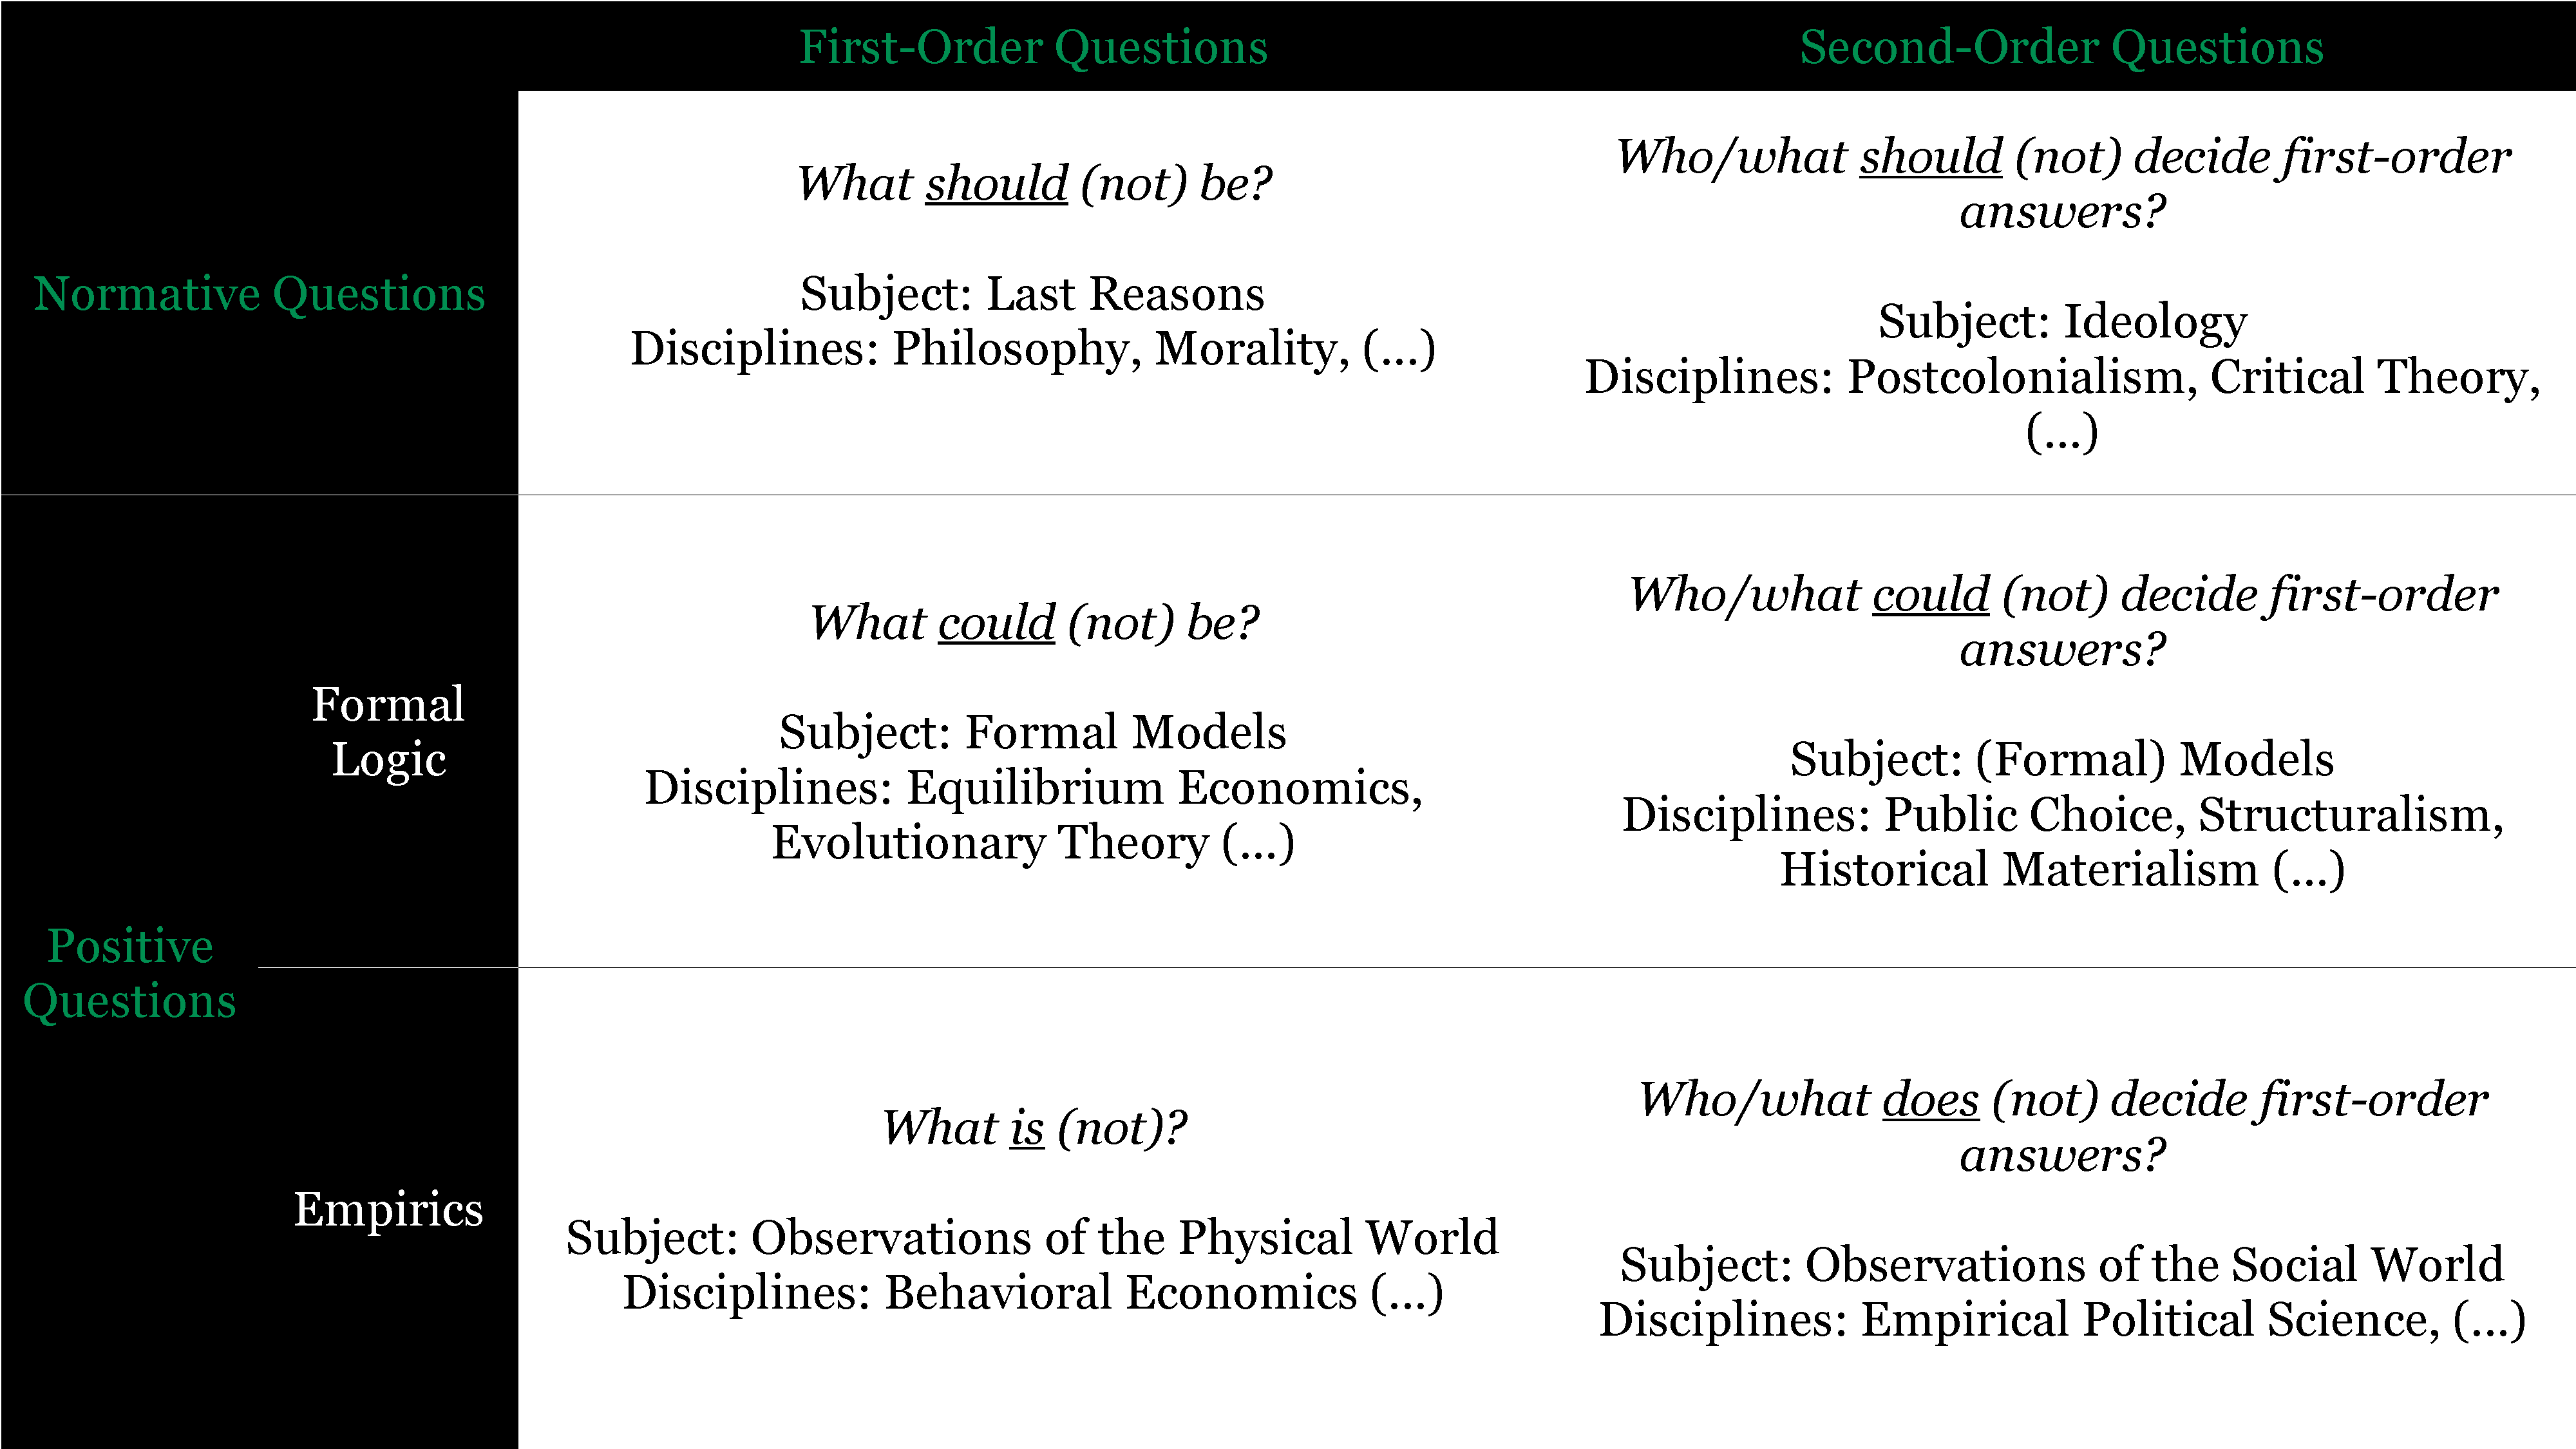
\includegraphics[width=1\linewidth]{orders-of-questions}  
	\caption{Overview of First, Second-Order, Normative and Positive Questions}
	\label{tab:1st-2nd-order-questions}
\end{table} 

The distinction between first-, second-order, normative and positive questions summarized in \autoref{tab:1st-2nd-order-questions} (p.~\pageref{tab:1st-2nd-order-questions}) matters for at least two reasons:

\begin{enumerate}
	\item 
	Clearly addressing one of these questions at a time, and striving to keep them separate makes for better social science. 
	With these categorically different questions come different goals, languages and methods. With blurring or negating these categories come ``politics-based evidence making'' (The Economist 2012), apolitical ignorance or both.
	\item 
	Because positive social science --- including this dissertation --- is out to explain the second-order decision on first-order questions, it must consider some first-order theory \emph{first}.
\end{enumerate} 

\subsection{First Order Theory \emph{First} \label{sec:1st-questions-first}} 
I am ultimately interested in the second-order questions of welfare, taxation and democracy, but proceeding by the method of elimination, I must first ask and answer the first-order questions: what \emph{should} and \emph{could} welfare, taxation and democracy look like.

Consider the two alternatives, that I must rule out before any second-order questions can be raised:

\begin{description}
	\item[No Desirable Hypothetical.] 
	If I could find only the presently observed design of welfare, tax and democracy to be at least somewhat desirable, there would be no social conflict to be explained, much like there is no need for a political science of wearing sunscreen. 
	(I partly take this \hyperref[sec:axiology]{later}, p.~\pageref{sec:axiology}).
	
	In the crime story metaphor, if the corpse in question had previously run amok shooting innocents, rupturing that persons coronary artery with a bullet might be have been self-defense or the last resort, and the only desirable course of action. 
	No \emph{further} criminal investigation may be necessary.
	
	\item[No Doable Hypothetical.] 
	If I could find only the presently observed design of tax and democracy to be materially doable, there would be no social conflict to be explained, much like there is no need for a sociological theory of gravity. 
	%here, too: I partly take this back later ...
	
	In the crime story metaphor, if said deceased suffered from an irreparable birth defect that caused the heart failure, no outcome but death is materially possible. 
	In that case, too, no criminal investigation will be necessary.
\end{description}
%add table here to further explain these. crosstab it.

Conceiving such to-be-ruled-out hypotheticals raises normative (desirability) and positive (doability) questions of the \emph{first}-order. 
These first-order questions cannot, as I explained above, be answered by social sciences (alone), but I must instead reference other disciplines, much like a detective hears forensic evidence.

If these ancillary disciplines reveal one, or several such desirable and doable hypotheticals that I cannot rule out, the non-occurrence of such hypothetical welfare, taxation and democracy beg a second-order explanation just as the observed arrangement requires explanation. 
In fact, the two are the same thing: to explain the presence of the present arrangement is to explain the absence of all absent arrangements. 

For illustration, consider the inverse scenario, in which I find no desirable and doable hypotheticals in welfare, taxation and democracy. 
If that were the case, there would be no second-order decision to be explained, because without such hypotheticals, there is no human choice.

If however, there \emph{are} desirable and doable hypotheticals, any second-order question always invokes these hypotheticals.

\subsection{Fallacies and Risks}%better title: glass full empty?
To be sure, this reasoning is not logically watertight and might turn into an argument from ignorance: even if I find no reason why hypotheticals should, or could not be, they might still be undesirable or impossible for some other reason. 
Absence of evidence, here, too, does not constitute evidence of absence. 

The same problem must plague medical forensics: no evidence of natural death does not prove a violent death and any conclusion to the contrary might cause an unnecessary murder investigation. 
In practice, this possible fallacy simply raises the question of where you place the burden of proof, because you can err either way: if you take absence of evidence of violent death as evidence of natural death, you might foreclose a necessary investigation and let someone get away with murder. 
Tellingly, when it comes to human corpses we place the burden of proof on the status quo: if the cause of death cannot be established --- if there is \emph{no} evidence of natural death --- the prosecution customarily opens an investigation.%find source for this

The positive social science of welfare, tax and democracy seems to have adopted a somewhat laxer standard. Here, much empirical work implicitly places the burden of proof on the hypothetical: without evidence that the hypothetical is normatively desirable and materially possible, the fundamental status quo of welfare and tax needs no social explanation. 
Conveniently, as hypotheticals go, they rarely produce conclusive evidence of their desirability and doability. Maybe, this is just the skepticism that positivism calls for --- or maybe, \hyperref[chap:hypotheticals-matter]{hypotheticals matter}, and such social science invariable turns latently affirmative (\autoref{chap:hypotheticals-matter}, p.~\pageref{chap:hypotheticals-matter}).

Either way, I here place the burden of proof on the status quo. 
If I find no reasons to the contrary, I assume that there \emph{are} several doable and desirable designs of tax and democracy, and require social science to explain the \emph{absence} of all but the presently observed design. 
If we apply the standard of forensics, any second-order theory of social change must be able to explain how the social conflict under study resulted in the non-occurrence of these alternative designs, especially the attractive ones.

I still want to shoulder part of the burden of proof. 
In tax, I can only plausibilize the hypotheticals by reviewing reputable work by others, and deduce my case from reasonable assumptions about human nature, and the economy. 
I must rely mostly on a \hyperref[itm:rationalism]{rationalist} epistemology (p.~\pageref{itm:rationalism}). 
Natural experiments --- the \hyperref[itm:empiricism]{empiricist} gold standard --- are unavailable, and all others suffer from limited external validity: a modern economy does not fit in the laboratory and equilibrium simulations poorly model such inframarginal institutional changes. %more on this somewhere else. Should explain why I can't look into tax in another way! Reference this section here.
In democracy, I similarly plausibilize the hypotheticals, but I can also point to and undertake some preliminary experimental tests.

To suggest, as I do, that there are desirable and doable hypotheticals in tax and democracy, must remain a preliminary proposition open to falsification. 
To the \citeauthor{Popper1934}ian scientist, there is always some absence of evidence, and therefore, no evidence of absence. 
If these particular hypotheticals turn out to be undesirable or impossible, so collapses any second-order hypothesis I might wager later, but, I hope, we will still have learned something.

Not only the advancement of science depends on such falsification, the history of progressive causes is also littered with what might charitably be called ``false positives''. 
My chosen hypotheticals --- deliberative democracy and progressive taxation of (unimproved) land value and (postpaid) consumption, too, may inspire such false hopes. 
They, too, should be approached with great care, especially, when they necessitate constitutional or otherwise reform of liberal democracy, as deliberative democracy may one day do. 
Tax reform, at least, should be open to falsification and is not an end in itself, especially because it thoroughly hinges on economic contexts and human motivation. %or maybe, deliberation is an end in itself, as a school for democracy

Then again, by any historical standard --- once-hypotheticals failed (for example, socialism) and successful (for example, universal suffrage) alike --- here are some fairly incremental reforms as carefully liberal in their \hyperref[sec:axiology]{normative axioms} (p.~\pageref{sec:axiology}) as they are conservative about \hyperref[sec:ontology]{ontological possibilities} (p.~\pageref{sec:ontology}).

\section[Axiology]{Axioms for Desirable Hypotheticals} \label{sec:axiology} %or last reasons?

\begin{quote}
	\emph{``I believe in clear-cut positions. I think that the most arrogant position is this apparent, multidisciplinary modesty of \emph{`what I am saying now is not unconditional, it is just a hypothesis,'} and so on. [\ldots] I think that the only way to be honest and expose yourself to criticism is to state clearly and dogmatically where you are. You must take the risk and have a position.''}\\
	--- Slavov \citet[45]{Zizek2003}
\end{quote}

Normatively desirable hypotheticals are preferable to others if we assume a basic humanist, or critical intention of positive social science and policy analysis to improve human lives.
	
From a strictly positivist point of view, this is the flimsiest of epistemological decisions I take: we might learn just as much about the social world from the nonoccurrence of bad outcomes, as from the nonoccurence of good outcomes
\footnote{
	For example, \citeauthor{Tilly-1985-aa}'s work on the genesis of the state might be construed as learning from the (almost) no-longer-occurence of \citeauthor{Hobbes-1651-aa}ian anarchy. 
	He might have said --- although he presents his argument differently --- that the un(!)-desirable hypothetical of atomistic war is no longer observed because, luckily, through a process of extraction and violence-production, supercharged by economies of scale, once fearsome racketeers nilly-willy evolved into states with an effective monopoly on the legitimate use of force \citep{Tilly-1985-aa}.
}.

My bias for desirable hypotheticals might be epistemologically arbitrary, but it is --- again --- pragmatic: there may just be so many undesirable, but doable counterfactuals (why \emph{not} return to workhouses rather than welfare, tariffs rather than taxation and mob rule rather than liberal democracy?) that it becomes plainly easier to pick amongst the supposedly fewer, attractive hypotheticals. 
Moreover --- if mostly implicitly --- modernization theory, (structural) functionalism and related traditions might have convincingly explained away some of those graver regresses of civilization. 
Lastly --- only slightly tongue-in-cheek ---, on a second look at the factual horror chamber of welfare, tax and democracy, there might not be \emph{that} many even less desirable, doable hypotheticals left. %I return to this glass-half-full-vs-half-empty debate later ... reference

What then, makes for desirable hypotheticals?

Emphatically, hypothetical tax, welfare and democracy, and with them, this research, hinge on last reasons.
Desirable tax and welfare are rational, efficient and fair. 
Democracy, too, must be these things and more: emancipatory, equal and deliberative. %change later.

Unfortunately, these last reasons sometimes conflict, and they do not even flow from any single ethic. 
What makes my hypothetical tax, welfare and democracy desirable is, instead, a hodgepodge of mongrels from quite distinct normative theories. 
I here list five of them and show how they apply to taxation, welfare and democracy:

%in all of this, I am completely leaving out all meta-ethical questions, as in: http://en.wikipedia.org/wiki/Meta-ethics (and maybe that's ok).

\begin{description}
	\item[Virtue Ethics \label{itm:virtue}]
	Tax, welfare and democracy are not desirably merely to the extent that they constitute, or foster \emph{virtue} inherent to human action and character (from \citeauthor{Aristotelesa}, \citeauthor{Plato}, \citeauthor{St.ThomasAcquinas1274} to \citealt{schwartz2006practical}). 
	At least under neoclassical dictum, tax and welfare are desirable to the extent that they \emph{do not} depend on, nor improve human virtue, but efficiently orchestrate our selfish demons \cite[compare][]{Smith-1776-lq}. 
	Liberal democracy, similarly, is desirable to the extent that it sidesteps questions of personal virtue and guarantees an agnostic process for all people, no matter the quality of their character \cite[compare][]{Dahl-1989-aa}.
	
	And yet, I rely on virtue ethics when I praise markets and states for letting us reap \hyperref[sec:nonzero]{non-zero-sumness} (p.~\pageref{sec:nonzero}), that supposed destiny of our nature \citep[for example,][]{Wright2000}. 
	The case for deliberative democracy, too --- as all virtue ethics --- implies a \emph{telos} of human life, to the extent that it posits intersubjective understanding or \emph{communicative action} as a last reason \citep{Habermas1984}.%add href sometime later?
	
	\item[Consequentialism \label{itm:consequentialism}] 
	Tax, welfare and democracy are also not desirable merely by the outcomes they produce, be they utility \citep{Bentham1789,Mill1863} or even self-interest \citep{Rand1957}. 
	Attractive consequences, especially different aggregate functions of utility
\footnote{
	For example, logarithmically diminishing returns to wealth, according to \cite{Bernoulli1738}.
}
go a long way to justifying taxation and welfare, but I would not bet the farm on them. 
	Even if, say, relative inequality were empirically unrelated to ``subjective happiness'' (as \citealt{KalmijnVeenhoven-2005-aa} seem to imply), %check this reference 
	and progressive taxation therefore not a maximizer of aggregate happiness, at least two other reasons would remain:
	\begin{enumerate}
		\item 
		Straightforwardly, we might wish to maximize consequences \emph{other} than some measure of hedonistic gain, including equality, growth, knowledge or liberty. 
		
		Utilitarianism --- as other consequentialisms --- side-step entirely the question of how the desired consequences would be measured, and who would do the observing
		\footnote{
			Similarly, utilitarianism characteristically side-steps the \emph{distribution} of utility. For example, \citeauthor{Mill1863} famously suggested to maximize ``the greatest good for the greatest many'', which might be understood to imply constant marginal returns, thereby equating equity with efficiency.  Before him, \citeauthor{Bernoulli1738} suggested that utility might be a logarithmic function of wealth, implying diminishing marginal returns. Crucially, no matter the specific aggregative function, utilitarianism reduces   \emph{distributive justice} to a merely positive question about human psychometrics, from which one or another \emph{hedonic calculus} \citep[originally][Chapter 4]{Bentham1789} must follow.
			
			I return to these, and other distributive norms when I discuss  \hyperref[sec:tax-optimality]{optimal taxation} (p.~\pageref{sec:tax-optimality}).
		}.
		Utilitarianism merely posits an \emph{ideal observer} \citep{Rawls1988} --- such as \citeauthor{Veenhoven-2000-aa}'s subjective happiness --- and does not allow us to problematize the conditions under which consequences are enumerated, or measured
		\footnote{
			John \citeauthor{Rawls-1971}, ever the critic of utilitarianism, has instead suggested an \emph{ideal}, \emph{original position} under which these decisions can be fairly made.
		}.
		\item 
		More fundamentally, progressive taxation --- or some other policy --- may remain attractive not because of \emph{any} distribution or measurement of consequence, but because equality might be inherently \emph{virtuous}, or the goods it can buy (including universal health care) may be a matter of \emph{deontological} rights.
	\end{enumerate}
	
	The consequentialist case for democracy is even thinner: as \citet[176]{Dahl-1989-aa} reminds us, equal intrinsic worth of humans \emph{alone} might be achieved by a benevolent dictator. Only in conjunction with (deontological? virtuous?) personal autonomy does it require democratic rule. 
	
	And yet, hypotheticals about taxation and welfare, and even democracy cannot ignore consequences, especially \hyperref[sec:tax-optimality]{aggregate utility} (p.~\pageref{sec:tax-optimality}) and its \hyperref[sec:tax-justice]{fair distribution} (p.~\pageref{sec:tax-justice}).
	
	\item[Deontological Ethics \label{itm:deontological}] 
	Tax, welfare and democracy are also not merely desirable to the extend that they abide by some set of absolute rights and duties. 
	
	On the one hand, most such deontological ethics are not specific enough to inform choices of tax, welfare and democracy. 
	For instance, the Golden Rule --- \emph{do unto others as you would have done to yourself} --- may not tell us much about what we should tax, when we should intervene in the market or how we should count votes. 
	\citeauthor{Kant1781}'s similar categorical imperative is equally mum on these matters, maybe because his is a philosophy and %expand?
	deals with \emph{man} in the singular, not \emph{men} in the plural as \citeauthor{Arendt1958} demanded of political theory
	\footnote{
		Writes \citeauthor{Arendt1958}, maybe \emph{the} proto-deliberative theorist: 
		\begin{quote}
			\emph{``Ohne Gleichartigkeit g\"abe es keine Verst\"andigung unter Lebenden, kein Verstehen der Toten und kein Planen f\"ur eine Welt, die nicht mehr von uns, aber doch immer noch von unseresgleichen bev\"olkert sein wird. Ohne Verschiedenheit … bed\"urfte es weder der Sprache noch des Handelns für eine Verst\"andigung.''}\\*
			--- Hannah \citet{Arendt1958} %page missing 
		\end{quote}
		And, similarly, in the english translation:
		\begin{quote}
			\emph{``Men in plural [\ldots] can experience meaningfulness only because they can talk with and make sense to each other and themselves.''}\\*
			--- Hannah \citet[Prologue]{Arendt1958} %page missing 
		\end{quote}
	}.
	Natural rights theories (from \citeauthor{Grotius1625}), be they liberal (from \citealt{Locke1689a} to maybe \citealt{Rawls-1993-aa}), spinoff (right-)libertarian (diverse, prominently \citealt{Hayek1944}, \citealt{Nozick1974}) concerned with negative freedoms \emph{from} (for example, false imprisonment), or positive freedoms \emph{to} (for example, human dignity, both \citealt{Berlin1969}) provide more guidelines, but they, too, are limited.
	Natural rights theories, and especially liberalism, set outer limits on what a government or person must not do \emph{to}, or must not fail to do \emph{for} the bearers of these rights, but they are too digital for a normative ethic of welfare, taxation and democracy. 
	For example, market interventions may be either permissible (freedom-to) or illegitimate (right-libertarianism), but natural rights do not offer much qualifications in-between. 
	It is of course the great appeal of natural rights that they are unconditional (as in: \emph{``Human dignity shall be inviolable''}, German Basic Law 1948) and pre-social (as in: \emph{``\ldots that all men are created equal''}, US Declaration of Independence 1776), but that makes them a little too lofty for inherently social, and contingent institutions as welfare and taxation. 
	There may, for example, be many (or no) taxes that allow for \emph{life, liberty and the pursuit of happiness} (\emph{ibid.}), but it would be a stretch to argue that these natural rights are best respected or least harmed by any particular tax on consumption, income or wealth. 
	Crucially, too, many collective decisions in late capitalism must balance one persons liberty, against another persons pursuit of happiness, or similar rival natural rights. 
		
	Contract theories (from \citeauthor{Hobbes-1651-aa}, \citeauthor{Rousseau1762} to \citealt{Rawls-1971}) are more specific still, by prescribing a decision-making process or condition to balance and protect rival rights. 
	While this may suffice to specify a desirable democracy (authoritatively \citealt{Dahl-1989-aa} on \emph{liberal}, \emph{pluralist} poliarchy), contract theories still recede into procedural norms on taxation and welfare. \citeauthor{Dahl-1989-aa} --- but not \citeauthor{Rawls-1971}, as we shall see! --- may inform us about how we should decide between, say, an income or a consumption tax, but abstains from substantive judgement. 
	When, however, the very quality of the (second-order) decision process over these tax choices is in question --- as it is in this dissertation --- evaluating first-order hypotheticals by a procedural standard risks infinite regress: a tax is good if the process was good, and the process is good if the tax is good, which is good if \ldots and so on.
	
%consider including the visualization about euler diagrams and production possibility frontiers in here?

	On the other hand, tax and welfare especially, are institutions that negotiate and trade off competing rights and duties, rather than strictly abide by them. 
	Natural rights to, say, property \emph{and} health care, offer no all-or-nothing propositions in taxation. 
	Instead, one tax may encroach \emph{less} on property than another, or at a greater (utilitarian) gain in health care than another. 

	In sum, deontological ethics, and especially its popular, liberal, contractual and procedural representatives are both not specific enough, and too demanding for desirable hypotheticals in welfare, taxation and democracy. 

	And yet, I cannot do without deontological ethics, especially not without liberalism. 
	Even if governments \emph{could} expropriate some owners at supposedly minimal welfare losses --- as the Eurogroup has allowed (encouraged?) the Cypriot government to proceed in 2013 with big savers --- it should not do so (nor be allowed to), because protection of confidence is a deontological right. 
	Similarly, even if democratic rule found executive pay excessive, and anticipated no \gls{DWL} fallout, it should not --- as Switzerland did in 2013 --- regulate \emph{uncoerced exchanges} \citep{Nozick1974} even between CEOs and shareholders, when a less intrusive policy (tax!) is available, simply because liberal states do not do that. %find better, thesis-related examples

	

	\item[Ethics of Care\label{itm:ethics-of-care}] 
	Lastly, tax, welfare and democracy are, for the most part, \emph{not} desirable because they establish caring relationships, as some (difference?) feminists have demanded \citep{Noddings1984,Gilligan1982}. 
	Whether we like it or not --- in fact, we \emph{should} like it --- our world is ruled by abstractions, too, and to these must respond our institutions of tax, welfare and democracy. 
	Absent a regress to lower, poorer levels of functional differentiation --- or some yet unforeseen explosion in human capacity --- we depend on wide-ranging abstractions such as a price system to orchestrate at least some of our relationships by mutual self-interest
	\footnote{
		I later return to medium-term dependence on such arguably impoverished interactions in \hyperref[sec:modernity]{modernity} (p.~\pageref{sec:modernity}) and suggest a \hyperref[sec:contingent-homo-economicus]{\emph{contingent} homo economicus} (p.~\pageref{sec:contingent-homo-economicus}).
	}. 
	Ethics of care govern \emph{individual}, \emph{concrete} and \emph{personal} relationships, and not those anonymously expressed in price signals, or some other abstraction. 
	Taxation, welfare and democracy, however, \emph{have} to ontologically respond to such abstractions, and to that extent, cannot be informed by a normative ethic that insists otherwise.
	
	And yet, I cannot abandon an ethic of care entirely. 
	For once, \emph{caring} reminds me that we may have other, more intimately personal capacities (or duties?) for goodness and desirable taxation, welfare and democracy may consequently have to leave room for caring to flourish. 
	For example, I imply an ethic of care when I later suggest that taxation should respect the promises of (mutual) care in marriage and family and not discourage, nor commodify such unions. %add \href
	More broadly, a good welfare system might have to carve out realms where such necessarily \emph{priceless} care can be extended --- not \emph{exchanged}! --- and might have to reallocate resources to those, especially women, who spend much of their energy caring for others, without compensation. 
	Something akin to ethics of care are also implied by some proponents of deliberative democracy, maybe including those who stress the importance of story-telling in democratic participation \citep{Poletta2006}. 
	Deliberative formats may also raise ethical questions of care simply because they make people engage with other people. Intersubjective understanding certainly requires the kind of personal relationships to which ethics of care supposedly apply.
\end{description}


I know then, that I know nothing --- at least nothing consistent --- about what makes tax, welfare and democracy desirable. 
That might be a socratic moment, but not a happy one for me or this dissertation. 
It frustrates me that I can summarize these ethics only in the crudest of terms, and that I fail to synthesize them. 
Such ignorance is troubling, too, for research as this, based on a social science education as devoid of normative theory as mine: clearly, these theories matter for tax, welfare and democracy as for any scholarship about them. 
Tracking down the choices and controversies in tax, welfare and democracy to different ethics is important work that I have to do without, resting this work on quite murky foundations.

All I can offer is a modicum of argumentative transparency, by labeling any downstream axioms in tax, welfare and democracy with the roughly appropriate normative ethics from which they flow.

Because none of the above ethics are sufficient, but each of them necessary to formulate desirable tax, welfare and democracy, I subscribe neither to virtue, nor consequentialist, nor deontological, nor care ethics but pick and choose amongst them.
I guess that makes me an ethical pragmatist of sorts, if a confused one.

%for all the pragmatism, check \cite{Bohman1999}

\begin{description}
	\item[Pragmatic Ethics \label{itm:pragmatic-ethics}] 
	--- not identical with pragmatism, and never to be confused with realism or \emph{Realpolitik} --- may best enumerate what makes tax, welfare and democracy desirable, for at least two reasons:
	\begin{enumerate}
		\item 
		In pragmatic ethics, morality can progress over time \citep{Dewey1932}, much as science advances through iterative inquiry. 
		Such tentative morality implies neither relativism, nor inaction: there may still be absolute values out there, we just cannot be sure that we have distilled them yet, but should act on whichever approximation we have tentatively arrived at.
		
		Tax, welfare and democracy, too, are such inherently tentative and contingent enterprises. 
		For example, when comprehensive income taxes were introduced to more neatly bifurcated class societies, the ethical quandaries of taxing labor and capital incomes might not have been foreseeable: labor income generally accrued to poor workers, capital incomes to rich capitalists, end of story. %add href.
		Similarly, as universal suffrage was wrung from the \emph{ancien regimes} and liberal democracy enshrined to fend off mob rule around the same time, the limits of a merely electoral and pluralist democracy in a complex world might not have been conceivable. 
		So too, no doubt, will the reforms of tax, welfare and democracy I suggest here reveal their blind spots, come progress.
		
		Acknowledging that our moral understanding may be imperfect, or even somewhat historically contingent, also in no way restricts us to the status quo under which this understanding was reached. Pragmatic ethics can be quite radical, maybe \emph{because} it accepts its own tentativeness and contingence: we can ``transform the character of our relation to social and cultural worlds we inhabit rather than just to change, little by little, the content of the arrangements and beliefs that comprise them.'' \citep[6-7]{Unger2007}. 
		I am inspired by such \emph{anti-necessitarianism} \citep{Unger1987}, even if --- or because? --- tax, welfare and democracy are not the stuff of revolution, but rather the ``indispensable if insufficient [\ldots] piecemeal and cumulative change in the organization of society'' \citep[xix]{Unger1987}. 
		I am keenly aware that especially reformed tax and welfare, but even deliberative democracy will, at best, progress us a little further to a point where we --- probably our progeny --- can better conceive morality, and undertake further tentative transformations we cannot even dream of.
		
		\item 
		Pragmatic ethics are also, as the name implies, intensely practical. Pragmatic ethics cannot be conceived of in other than practical terms: 
		\begin{quote}
			\emph{``Consider what effects, that might conceivably have practical bearings, we conceive the object of our conception to have. Then, our conception of these effects is the whole of our conception of the object.''} \\*
			--- \cite[293]{Peirce1878}
		\end{quote}
		This \emph{pragmatic maxim}, as it became later known, works well, especially for tax and welfare. 
		The proverbial proof of their ethical pudding, too, lies in the eating. 
		For example, a tax on income or consumption becomes good or bad greatly by how it works in practice: what \hyperref[itm:virtue]{virtues} it curtails, what \hyperref[itm:consequentialism]{utility} it wastes or what \hyperref[itm:deontological]{rights} it hurts --- very little of which can be read in the Platonic idea of either of those alone.
	\end{enumerate}		
\end{description}

Admittedly, such pragmatic ethics are fairly amorphous, and they do not constitute any of the clear-cut positions that \citeauthor{Zizek2003} demand in the above. 
They merely provide the normative theory under which I can organize, and justify the following hodgepodge of axioms for desirable hypotheticals in tax, welfare and democracy. 
Here then, are my positions.

\subsection[Liberal]{Liberal Limits and Procedure} \label{sec:liberal}
Desirable hypotheticals in tax, welfare and democracy are liberal. 
They do not infringe on the most extensive basic liberties compatible with similar liberty for others \citep{Rawls-1971}, a liberal formulation of the \emph{Golden Rule} of reciprocity. 
These include the political and civil liberties enshrined in various liberal constitutions, but, following \citeauthor{Rawls-1971} \emph{do not} extend to unencumbered private property of the means of production or unlimited freedom of contract, as libertarians would have it.

Desirable hypotheticals in tax, welfare and democracy must be liberal both in the substance of, as well as in the process by which they bring social chance. 

Substantively, these regimes must not constrain the lifestyles of people, except if and to the extent that such choices conflict with --- as \citeauthor{Rawls-1971} posited --- the choices others. 
This is, for example, a very real concern in making consumption taxes progressive, or in taxing savings, both without dictating consumption baskets or prescribing a financial biography. %add href 
Similarly, democratic fora should encourage  ``\emph{alternative} conceptions of the common good'' \citep[18, emphasis added]{Cohen-1989-aa} rather than promote a specific social change, even if such a coherent scientific agenda \emph{could} be found. 
This insistence on a plurality of lifestyles and ideas of the good distinguish a desirable hypothetical from totalitarian zeal and hermetic ideology.

Procedurally, desirable hypotheticals rely on democratic advocacy, not armchair guardianship to become real. 
No matter, say, the \hyperref[itm:consequentialism]{consequentialist} (p.~\pageref{itm:consequentialism}) value of a \gls{PCT}, its introduction must respect, as \citeauthor{Dahl-1989-aa} has highlighted, \emph{both} (\hyperref[itm:deontological]{deontological}!) intrinsic equality \citeyearpar[84]{Dahl-1989-aa} \emph{and} (liberal!) personal autonomy \citeyearpar[97ff]{Dahl-1989-aa}. In his influential formulation \citep[109ff.]{Dahl-1989-aa}, it can only be realized by a democratic process marked by at least:
\begin{enumerate}
	\item effective participation, 
	\item voting equality at the decisive state, 
	\item enlightened understanding and, 
	\item control of the agenda and 
	\item inclusiveness %not sure about this last one %Equality must extend to all citizens within the state. Everyone has legitimate stake within the political process.[citation needed] 
\end{enumerate}

These criteria imply a fairly conventional catalogue of \emph{negative} rights, or freedoms \emph{from} and a standard formulation of democratic process (but not substance). 
Together, these liberal norms take precedence over any of the other, below axioms for desirable hypotheticals: in \citeauthor{Rawls-1971}'s formulation for his \emph{Theory of Justice}, violations of any of these rights ``cannot be justified or remedied by other [...] advantages'' \citeyearpar[81]{Rawls-1971}. 
They cannot be traded off other benefits, but can only be limited when they come in conflict with one another, as for example, freedom of speech and defamation legislation may.  %might refer to later section on justice
%reference, include visualization? 

I posit these rights \hyperref[sec:deontological]{deontologically}, but I also think \hyperref[itm:pragmatic-ethics]{pragmatically} (p.~\pageref{itm:pragmatic-ethics}) that for the foreseeable future, these norms may be our best, if tentative and minimal bet of what people and government should \emph{never} do to people. 
Maybe, liberal and other deontological norms can also serve under some kind of precautionary principle in ethics: given at least some uncertainty over, or contradiction within other normative ethics --- especially consequentialism --- we should accept liberal limits to policy because they might help reduce some downside risks.

\subsection[Rational]{Rational Preferences} \label{sec:rational} %does this work, given that the below is also about utility? 
Desirable hypotheticals in tax, welfare and democracy are based on and help people express rationally coherent preferences.

\cite{VonNeumannMorgenstern1944} have axiomatized rational coherence thus:
\begin{description}
	\item[Completeness \phantomsection \label{itm:completeness}] For any two alternatives, $A$ and $B$, we either ordinally prefer $A$ to $B$, or $B$ to $A$ or are indifferent between $A$ and $B$.
	\item[Transitivity \phantomsection \label{itm:transitivity}] For every three alternatives $A$, $B$ and $C$, where we prefer $A$ over $B$ and $B$ over $C$, we must prefer $A$ over $C$.
	\item[Continuity \phantomsection \label{itm:continuity}] For every three alternatives	$A$, $B$ and $C$, where we prefer $A$ over $B$ over $C$, there is a lottery comprised of a known number of $A$-lots and $C$-lots between which and $B$ we are indifferent.
		
	And, most controversially,
		
	\item[Independence \phantomsection \label{itm:independence}] If between two alternatives $A$ and $B$, we prefer $A$, given a third option, $X$, we still prefer $A$ over $B$.	
\end{description}

Such \gls{vNM}-rational actors can be said to have \emph{well-formed}, \emph{ordinal} preferences over given alternatives, and can, by \citeauthor{VonNeumannMorgenstern1944}'s work, express equivalent, unique and \emph{cardinal} preferences over these alternatives. 
That is, if an actor can \emph{rank} alternatives \gls{vNM}-rationally, she can also assign them a set of equivalent real numbers, such as willingness to pay. 
\citeauthor{VonNeumannMorgenstern1944}'s transformation of ordinal preferences into cardinal utility can be roughly imagined thus:
\footnote{
	Caveat: the mathematics escape me.
}
An agent is offered many lotteries with known probabilities of the alternative outcomes in question. 
If the agent is \gls{vNM}-rational, her ordinal preferences dictate her choice between \emph{any} such known probabilities revealing her \emph{expected} utility function, including those probabilities where she is indifferent between alternatives. %reword
Probabilities being cardinal, the agent's choices between them reveal her cardinal utility from the alternatives. A \gls{vNM}-rational agent's ordinal preferences can thereby always be expressed in some cardinal utility function, and vice versa: if an agent has a cardinal utility function over ordinally preferred alternatives, she must be \gls{vNM}-rational.

Crucially, cardinal \emph{utility} thus revealed need not be a linear function of some cardinal \emph{value}: agents \emph{expected utility} may differ from the \emph{expected value} of some outcome, where its value is merely multiplied by its probability. 
Agents, can, for example be risk averse and display a correspondingly concave utility function
\footnote{
	Maybe because they experience logarithmically diminishing returns to utility, as \cite{Bernoulli1738} suspected.
}. 

In the social sciences, expected utility theory --- as its brethren the first theorem of welfare economics --- often arouses great passions: it is either considered elegant and self-evident, or vulgar and misleading. 
Here too, I must briefly explicate its status:
\begin{enumerate}
	\item 
	Expected utility theory is \hyperref[itm:a-priori]{\emph{a priori}} knowledge (p.~\pageref{itm:a-priori}) of the first-order flowing from a \hyperref[itm:rationalism]{rationalist} epistemology (p.~\pageref{itm:rationalism}). 
	It implies no (first-order, empirical) observations of actual human decision making
	\footnote{
		In fact, \gls{vNM}-rationality has a fairly poor empirical track record. Behavioral economics, cognitive psychology and related empirical disciplines demonstrate that ``humans are not well \emph{described} by the rational-agent model'' \citep[K7094, emphasis added]{Kahneman2011}. 
		
		As far as these findings concern \emph{cognition}, they do not pose great problems. 
		Notably, the research in this field I am aware of does not suggest that humans would be \emph{categorically} incapable to be \gls{vNM}-rational, or form otherwise coherent preferences. 
		\citeauthor{Kahneman2011}, for one, suggests that we think fast but sloppily most of the time (under ``system I''), but can also think slowly and thoroughly (under ``system II''). 
		In fact, prospect theory and other behavioral economics proceed by comparing actual human decisions to \emph{a priori} \gls{vNM}, or otherwise rational choice. 
		If no one else, at least the people doing this research must be able to think rationally.
		
		I \hyperref[sec:ontology]{ontologically} (p.~\pageref{sec:ontology}) accept these conditional limits of human rationality and suggest --- as \citet[K7094]{Kahneman2011} --- we build \emph{rational} institutions that help us make better decisions (p.~\pageref{sec:contingent-homo-economicus}).
	}
	.
	%, nor does it suggest any (second-order, normative) prescriptions of how people should decide. 
	As other exercises in formal logic, it is not up to social scientific debate.
	\item 
	Expected utility theory invites \emph{no} intersubjective comparisons (such as those on which the first theorem of welfare economics rest). 
	Any talk of \emph{aggregate} expected utility is meaningless, absent additional assumptions. 
	That said, expected utility theory can provide no justification for any particular aggregation or comparison of individual utility, but once such aggregation has been accomplished on other grounds (for example, by democratic rule), it can posit rationality for and guide decisions based on such aggregated preferences.
\end{enumerate}

Why now, readers may ask, does any of this matter?

Expected utility theory matters a great deal for desirable hypotheticals in tax, welfare and democracy. 
In tax and welfare it suggests the very necessary and sufficient (!) conditions under which it even makes sense to speak of utility, or its manifold incarnations in (cardinal!) economics. 
Markets can work their hypothesized magic of pareto-optimization under the first theorem of welfare economics if, and only if people can express their preferences \gls{vNM}-rationally. 
If people displayed, say, preferences between good $A$ and $B$ depended on a luxury good $C$ becoming available in a market \citep{Frank2010a}, the whole intellectual artifice of ``utility'' and any pursuant neoliberal imperatives with it, may crumble. 
Tax and welfare may have to step in, to rectify the original irrationality. 
Conversely, to justify any of my desired welfare interventions into the market economy is to argue for enhanced expected utility: assuming (reasonably, I think), that people prefer an $A$ of no insurance premium, livelong health, to a $B$ of some insurance premium, cared-for sickness, to a $C$ of some insurance premium, livelong health, to a $D$ of no insurance premium, uncared-for sickness, but suggesting that, when they give the probabilities and their risk aversion some thought, people (should) find $B$ to be of maximal expected utility, is to invoke \citeauthor{VonNeumannMorgenstern1944}. 

The case is even clearer in democracy. 
On the one hand, \gls{vNM}-rationality specifies what can be accepted as ordinal preference inputs (votes), if their bearers (citizens) are to have some consistent expected utility in the face of risky choice (strategic voting!). 
On the other hand, these \gls{vNM} axioms must also be accepted by any democratic aggregation mechanism --- even if, absent meaningful intersubjective comparisons, \citeauthor{VonNeumannMorgenstern1944} cannot justify any particular mode of aggregation. 
As I hypothesize later, popular tax choice under pluralism may well be plagued by irrational, inconsistent preferences of voters, and suboptimal choice in tax may, in part, be attributed to an aggregation mode that exploits these flawed preferences. %add reference
Conversely, it appears that even assuming \gls{vNM}-rational voters, aggregative democracy alone may not be able to produce minimally attractive decisions. %add references

Expected utility theory not only serves me to elucidate such \emph{a priori} consequences, my normative conviction goes further and deeper. 
To speak of rationally maximizing utility, as I wish to do, \emph{is} to imply \citeauthor{VonNeumannMorgenstern1944}, at least for now. 
Without their axioms for rationality, we do not know what we are talking about when we say ``utility'', and conversely, without their formulation of utility, we do not know what we are talking about when we say ``rationality''. If the two are to mean anything, I suspect, they must be related in the terms that \citeauthor{VonNeumannMorgenstern1944} have worked out.

\subsection[utilitarian]{Pragmatic Utilitarianism} \label{sec:utilitarian}%this title also doesn't work well.

Desirable hypotheticals in tax, welfare and democracy maximize outcomes that are valuable to people.

Unfortunately, such a utilitarian axiom raises more questions than 
it answers, including: 
\begin{enumerate}
	\item \label{itm:aggregation} How do we aggregate value over different people?
	\item \label{itm:utility} How can we know what people value?
\end{enumerate}
I cannot explore these questions in full, let alone answer them. 
Yet, to suggest desirable tax, welfare and democracy \emph{without} raising these questions would be charlatanry.
Without at least a tentative and pragmatic response to these questions, there can be no meaningful talk about their \hyperref[itm:consequentialism]{consequences} (p.~\pageref{itm:consequentialism}).

Question \ref{itm:aggregation} is easier to dismiss (if not answer), so I will deal with it first.

\subsubsection[Aggregation]{The Problem of Aggregation\label{sec:aggregation}} 

Utilitarianism runs into an empirical, or even ontological problem when it comes to aggregating value over different people: it posits an ideal observer capable of comparing value between people
\footnote{
	Only consequentialist ethics that rely on \emph{subjective} consequences run into this problem. 
	A (state) consequentialism seeking to minimize, say, CO2 emissions, is defined in aggregate terms already. 
	If minimal emissions are \emph{the} last reason, it does not matter, for example, who sacrifices how much.
	Of course, it would be hard to justify such a consequentialism with no reference to subjective consequences and it may become arbitrary.
}
. 
Sadly (or not?) such an ideal observer is not readily available \citep{Rawls1988}, and we do not even know whether such intersubjective comparison is ontologically possible.

This is not to say that absent an \emph{ideal} observer, we are off the hook. We \emph{should} care about other people with whatever roundabout empathy we can muster, but, strictly speaking, we should \emph{not} do it for utilitarian reasons. 
The last reasons for which we should care about the consequences of others are precisely not consequentialist, but may be, for instance, deontological (equality!), virtuous (charity!) or caring (empathy!). %add hrefs

Utilitarianism \emph{cannot}, as \cite{Bentham1789} might have hoped, reduce distributive justice to an empirical question, it can merely provide the cardinal language in which we can ask about taxation and welfare. 
Still, as I have argued \hyperref[sec:consequentialism]{above}, only (cardinal) utilitarianism can speak to the kind of aggregation that especially taxation and welfare require.%find href? 
What we must do then, is to problematize --- not presume --- ideal observation, as \citealt{Rawls1988} has demanded. In his \emph{Theory of Justice},
\citeauthor{Rawls-1971}, too, has suggested the mode for such observation that I choose here, and discuss further \hyperref[sec:fair]{later} (p.~\pageref{sec:fair}).

\subsubsection[Utility]{The Problem of Utility} \label{sec:utility}

Question \ref{itm:utility} on utility is even thornier. 
Behavioral economics, decision science and related disciplines present empirical findings that question whether humans have any \emph{consistent} sense of utility, let alone a cardinal one. 
This poses much harder questions for institutional design than the cognitive heuristics and biases, because from a utilitarian perspective there can be no such a thing as ``flawed emotions''.
Whatever people \emph{feel} --- no matter how inconsistent --- are the last, and only consequences about which a utilitarian cares. Certainly to a utilitarian, flawed \emph{cognition} can and should be mitigated to improve its consequences, but there are no last reasons to correct human \emph{emotion}, precisely because these \emph{are} the last reason
\footnote{
	Readers may note that I allow utilitarianism to collapse a normative question into an empirical question --- a conflation that I later criticize in other arguments. %\href
	This conflation is, in fact, inherent to utilitarian arguments.
}
.

I cannot here discuss at length the empirical findings on human emotion, but illustrate the questions it raises drawing only on some of \citeauthor{Kahneman2011}'s findings in prospect theory. I suspect that related approaches will pose similar questions. In his recent summary, \cite{Kahneman2011} poses at least two empirical critiques of \gls{vNM}-like human utility:

\begin{enumerate}
	\item \label{itm:inconsistence}
		Humans express their utility in inconsistent, non-\gls{vNM}-preferences. 
		For example, people are not just \emph{risk averse} --- as a convex utility function might explain ---, they are also \emph{loss averse} \citep{KahnemanTversky1979}. 
		From any given reference point, they seem to reap more hedonic gain from avoided \emph{losses}, than from equally-sized missed \emph{gains}. 
		As people make choices, their reference points can shift, and with that, their preference over the original choice can even \emph{reverse}: \cite{KahnemanTversky1979} find that when people have acquired mugs, they often accept only selling prices \emph{higher} than their buying prices.
		
		All of this spells trouble for \gls{vNM}-consistent preferences, and especially cardinal utility --- or willingness to pay --- on which orthodox economics relies: prospect theory ``is in many ways the least satisfactory of those considered since it allows individual choice to depend upon the context in which the choices were made'' \citep[634]{Grether1979}.

	Such deviations from consistent utility may also affect judgments of fairness in real life labor markets, as \citet[L5248]{Kahneman2011} notes. 
	If confirmed, these findings may become relevant to macroeconomic policy and hypotheticals in welfare and taxation, too. 
	If, for example, a wage cut by any given amount causes more hedonic loss than a raise by the same, or even a higher amount creates hedonic gain, \emph{creative destruction} \citep{SchumpeterSwedberg-1942-aa} may not be a utility optimum, even if it nominally were a positive-sum gain
	\footnote{
		Note that current macroeconomic policy aims to curb exactly the kind of downward wage rigidity that we might expect from loss-averse workers.
		Inflation is set at a positive rate to hide \emph{real} wage cuts at \emph{nominally} constant rates.
		Of course, as buying power decreases, workers \emph{will} eventually experience some hedonic loss, even though they may not readily attribute it to real wage cuts.
		Speculatively, if loss aversion loomed large, as utilitarians, we should cherish (!) downward wage rigidity and make sure that it operates effectively, even if we thereby forego gains elsewhere in the economy.	
	}
	. 
	Instead, from a utilitarian perspective, a general bias to conservatism may be warranted.
	Similarly, taxation might have to be revamped to account for loss aversion.
	Speculatively, if people suffered inordinate hedonic losses when parting with market earnings, taxation might have to be \emph{less} progressive than otherwise desirable. 
	We might also have to \emph{time} taxation so that it minimizes the \emph{apparent} if not the real sense of loss. 
	For instance, withholding taxes at the source rather than a comprehensive \gls{PIT}, or generally indirect rather than direct taxes may be loss-aversively utilitarian, even if they were conventionally inefficient.
	
	Interestingly, then, the equity implications of loss aversion are unclear. 
	Clearly, however, the abstractions of orthodox economics, and with it, conventional desiderata for hypothetical tax and welfare, are incapable of adequately capturing prospect theory, or other non-\gls{vNM}-utility.
	
	\item \label{itm:undefined}
	More generally --- or equivalently? --- people may not only be unable to express consistent preferences, but there may be no such thing as well-defined utility, or subjective well-being.
	
	\citet[7056]{Kahneman2011}, for one, describes three different operationalizations of subjective well-being
		\footnote{
			\ldots not to be confused with the debate over happiness as a state, or a trait \citep[for example][]{StonesHadjistavropoulos-1995-aa}.
		}
		: 
	\begin{enumerate}
		\item \label{itm:experienced} Experienced well-being, reported \emph{as} hedonic states occur.
		\item \label{itm:remembered} Remembered well-being, reported \emph{after} some interval of hedonic states.
		\item Hypothetical well-being, reported as the hedonic gain or loss ascribed to some non-outcome
		\footnote{
			For example, a quadriplegic might be asked how much happier she would be without her medical condition.
		}
		.
	\end{enumerate}
	If there were \emph{one} such thing as subjective well-being, these three operationalizations --- and especially \ref{itm:experienced} and \ref{itm:remembered}, falsifiable \emph{within-subjects} --- should yield the \emph{same} hedonometer. 
	Trivially, remembered well-being should simply be the time-integral of experienced well-being.
	Alas, it is not, as people seem to ignore duration and instead remember some (peak-end) \emph{average} \citep[K7056]{Kahneman2011}.
	What then, do we --- and happiness researchers --- mean, when we talk about subjective well-being? Clearly, none of the operationalizations alone can be satisfactory (pun intended) \citep[see][K7056]{Kahneman2011}, but together, they do not add up to any \emph{one} concept: they are just inconsistent.
	Utilitarianism, and with it, orthodox economics and consequentialist hypotheticals in welfare, tax and democracy face another empirical dead-end.
\end{enumerate}


\subsubsection[Emptiness]{The Emptiness of Utilitarianism} \label{sec:emptiness}

These twofold empirical dead-ends of utilitarianism pose not merely academic conundrums, they raise very fundamental problems in welfare and taxation. Orthodox economics --- especially the welfare kind --- and many of the concepts I take for granted here all revert back to an empirically untenable assumption of \gls{vNM}-consistent, subjective consequences. 
To say that an economy grows is to say that the net subjective consequences of people are improving along their \gls{vNM}-preferences. 
To say that an economy has a positive savings rate is to say people are foregoing part of their \gls{vNM}-preferences now, and store them in some material (a house) or immaterial (a patent) form that will be \gls{vNM}-preferable in the future. 
To a utilitarian economist --- almost a pleonasm! --- there is no \emph{objective} value, other than \gls{vNM}-ranked \emph{subjective} preferences, handily reported as utility, or willingness to pay. %note that it's NOT prices, correct this -- the net of the two is the consumer surplus!
\footnote{
	This problem also plagues public choice and finance: to a utilitarian economist, there is \emph{no} known value to public goods (such as defense), because by definition, markets do not operate on public goods and can thereby not extract an exchange value to approximate subjective preferences over such goods.
	Instead, governments usually undertake some form of \gls{CBA} to make production decisions. 
	As part of such \gls{CBA} bureaucrats must assign (or survey) at least the supposed benefits. %reference to later fn on the problem of surveys
	
	This problem is readily apparent when comparing some macroeconomic indicators between countries, or even just over time.
	An economy-wide savings rate, for example, must either ignore publicly held fixed capital %proper term
	or statisticians must impute the value of these (ostensible) investments out of thin air.
	At least by the standards of exchange valuation, there is \emph{no} definitive value of, say, a public investment into basic research even though it would clearly be important to know about the expected future utility of these and other projects when gauging a savings rate.
}
\footnote{
	This problem may plague \emph{all} subjective theories of value in economics, whether defined by the labor saved by, or put into a good \citep{Smith-1776-lq,Ricardo1817,Marx-1867-aa}, or the utility enjoyed by the marginal consumer buying it and expressed in her willingness to pay \citep[for example,][]{Walras1874}. Either way, ``labor'' and ``marginal utility'' must be defined by \gls{vNM}-consistent preferences. 
	Labor, after all, is nothing but an unattractive choice, which we make in return for the right to make some other, more attractive choice. Similarly, being a marginal consumer is to say that relative to all other economic choices (say, another good), buying the good in question at the given price is a \gls{vNM}-preferred choice.
	
	This radically relative conception of subjective value has been criticized as circular reasoning: the ordinal preferences for a good over all other goods is determined by relative, cardinal price for all other goods, which in turn are determined by the ordinal preferences for each of those goods over all other goods \cite[confer][]{Mattick1978}.
}

There may then be no \emph{no} uncontested, objectifiable basis to value human choices and activity, as orthodox economics and much of the following desiderata in welfare and taxation. 
Even if we subscribe to utilitarianism, we may not be able to reduce desirability to an unambigous empirical question. 
\footnote{
	Entropy may be the one, unambigously physical phenomenon to measure human activity. 
	As per the second law of thermodynamics, entropy --- colloquially: disorder --- increases in any isolated system, including the universe.
	Life, however, \emph{internally} increases and maintains order, by consuming negative entropy, that is, increasing \emph{external} entropy elsewhere in the universe (for example, consider what our bodies do to a black forest cake as we metabolize it) \citep[confer][]{Schrodinger1944}.
	
	Valuable economic activity, too, may be conceived of as creating and maintaining order locally, by further increasing disorder elsewhere (for example, consider the human by-products of making a black forest cake).
	Incidentally, some sources of negative entropy for economic activity may be better than others, the carbon-cycle of our planet being a particularly poor choice to dump entropy.
	
	However, even if our local entropy-decreasing \emph{could} be measured, it would presumably leave much to be desired in the way of policy guidance.
	Building a planetary reservoir of frozen black forest cakes may be an impressive achievement in negative entropy, but people will probably get tired from the desert after a while.
	Maybe, even a physical concept as entropy can only serve as a necessary, but not a sufficient criteria for value: whatever of value we produce will probably be fairly ordered, but not everything ordered we could produce would be valuable to us.
	In other words, even physics cannot help us get around the utilitarian problem of subjective consequences.
}
Rather, it appears, asking about preferences, or other subjective consequences, always begs \emph{more} questions \citep[confer][]{Kahneman2011}, including about the \emph{kind} of preference consistency, or the \emph{kind} of subjective satisfaction --- about all of which we must find some kind of agreement. 

Empirically, then, desirability cannot be reduced to a measurement of \emph{pre-social} preferences, because these preferences, along with all that we may deduce from them, are only socially defined.
Willy-nilly, first-order inquiries into the utility of some choice have a habit of turning into second-order questions on the social conditions under which said utility was defined, measured and expressed. %redundant?

What then, are we to make of this emptiness of utilitarianism?

Should we just abandon it and go for other ethics, instead? Surely, some caution is warranted, and we should back up normative claims with other ethics, because if nothing else, utilitarianism runs into these empirical dead-ends
\footnote{
	Decision scientists \citep[for example,][]{Kahneman2011}, happiness researchers \citep[for example,][]{Veenhoven-2000-aa} and whoever else presumes and/or questions subjective consequences and so much as hints at normative implications should, if only for the sake of argumentative clarity, out themselves as closeted utilitarians.
}
.

I maintain that no matter these contradictions, we should stick to (some) form of utilitarianism, because normatively as ontologically, the world demands of us risky choices, that to choose one alternative is to negate another, and that as individuals and as societies, we must be willing and able to meaningfully trade-off desired outcomes. 
The only way to do this at a scale, and under risk is to compute, as best we can, expected utilities.
Welfare and taxation, especially, ontologically presume, as much as they seek to improve comparable and consistent self-reported consequences.
If we are to make meaningful normative choices between factual and hypothetical welfare and tax, we must have a notion of utility.

But --- is that not cheating? %maybe this should go into the later section
After all, I am justifying hypothetical taxation, welfare and democracy with last reasons that I know to be unconvincing, but posit them anyway because without them, I cannot justify hypothetical (or any!) taxation, welfare and democracy. 
Admittedly, I am cheating, but I like to call it ethical pragmatism, instead.
I accept that in utilitarianism, as elsewhere, our moral judgements may be imperfect and tentative, but, to progress to greater clarity, must rely on them anyway, for three reasons:

\begin{enumerate}

	\item 
		Pragmatically, we must rely --- in part --- on utilitarian ethics because, for now, we are ontologically as empirically faced with a world that --- in part --- works according to it.
		If you want to get something (deontologically?) good done today, you will probably have to appeal to popular notions of utility, no matter how ill-conceived they might be as last reasons.

	\item
		Pragmatically, it is a safe bet that whatever we will deem good in the future, will, among other things, probably require not only negative entropy, but more specifically, \emph{stuff} that people prefer, including shelter, food and clothing. 
		Of course, we may be less certain about many other things that people ostensibly now prefer --- luxury cars, computers carved out of solid aluminum, espresso machines --- and end up producing (future) utility, that does not hold up on (future) ethical reflection.
		Still, we should better be safe with \emph{some} attractive subjective consequences, rather than sorry without \emph{any} such utility.

	\item
		Lastly, and also pragmatically, we can further --- but not perfect --- our ethical understanding of subjective consequences by problematizing, then improving those very social conditions under which we empirically seem to be forming our preferences. %notably, the whole social influence literature is still missing in here. Might have to add that up top later. Actually, maybe that's ok, because I am dealing with a normative theory here, and merely test whether it's empirically possible. The social influence stuff might rather go into the ontology section.
		%!!! this is very important; both deliberation and taxation (PCT!) are actually institutions to improve this problem of isolation under utilitiaranism: it may help us to intersubjectively compare value, as well as to become clearer about what it means to ourselves.
		%!here is a crazy idea: maybe "erfahrungen auf vorrat" -- popular culture -- is in fact this; it's trying for us to get some better idea of how we might like different things, before, during and after the fact.
		If utility is, in fact, \emph{not} pre-socially given, we can meaningfully \emph{talk} about it.
		
		Of course, \emph{that} is cheating, too.
		By problematizing the social conditions of forming preferences, I have just reassigned a first-order question (utility) to second-order status, a move I otherwise despise.
		To do this in a normative ethic, is really just to rephrase the question: after all, to \emph{what}, if not a utilitarian standard, do you hold the social condition of preference-formation?
		
		I allow myself this trick not because it resolves the confusion, but simply to organize my discussion of welfare, tax and democracy.
		
		Welfare and taxation, are --- by definition --- the realms in which the social conditions of preference formation are \emph{not} problematized.
		Here, I ontologically assume, and normatively require preferences to be (largely) pre-social.
		
		Democracy, in turn, is \emph{the} social condition under which we form preferences in intersubjective deliberation
		\footnote{
			I return to this distinction when I discuss deliberative democracy in \autoref{chap:better-democracy} (p.~\pageref{chap:better-democracy}.
			Assuming and enabling social, rather than pre-social preferences is an important tenet of deliberative theory and practice. %nah, this can be better, more precise.
		}
		. 
		Here, I ontologically assume, and normatively require preferences to be (largely) social. 
\end{enumerate}

\subsection[Fair]{Justice as Fairness} \label{sec:fair}
Desirable hypotheticals in welfare, tax and democracy are just if they treat people fairly. 

Justice --- especially \emph{distributive} justice --- deals with \emph{men in the plural} as \citeauthor{Arendt1958} demanded of political theory, and regulates competing claims between people. 
As we have seen, some of the previous ethics tell us little about how to resolve conflicts \emph{between} different bearers of rights, virtue, consequences or care, respectively. 
Deontological liberalism provides some digital rules, but these tend to be either minimal, or overly restrictive.
Consequentialist utilitarianism promised to make aggregation an empirical matter, but cannot do so convincingly.
Crucially, neither of these ethics suggests how conflicts over the meaning of, or conflicts between competing claims can be resolved.

Here again, I turn to John \citeauthor{Rawls-1971} to provide a meta-standard for finding desirable hypotheticals.
 
In his influential ``Theory of Justice'', he provides that standard: \emph{justice as fairness}. 
Ever the liberal \citep[and similar to above-mentioned][]{Cohen-1989-aa}, he suggests \emph{no} definite desiderata, but instead proposes a thought experiment under which moral claims have to qualify to be admissible for consideration. 
In his thought experiment, \citeauthor{Rawls-1971} imagines an \emph{original position}, where deliberators know nothing about their endowments, status and power in the real world. 
Only moral claims that can be defended under such a \emph{veil of ignorance}, suggests \citeauthor{Rawls-1971}, may --- but need not be --- just.

Oddly, this imagined original position is \emph{almost} a liberal procedure for justice, or a normative claim of the \emph{second} order --- but not quite. %add href
The veil of ignorance, is, of course, materially impossible and operates only metaphorically. 
Justice as fairness, is, instead, an \emph{end-state theory of (distributive) justice} \citep[1007]{Fried1999}. 
Genially, Rawls has thereby crafted a standard of \emph{substantive} justice, avoiding both the contingency of immediate imperatives (``[shellfish] shall be an abomination to you'', Leviticus 11: 8, KJV), the nihilism 
\footnote{
	Walter \citeauthor{Benjamin1927} has revealed the nihilism of legal positivism: ``law-making (...) implies power (...) which implies violence'', \citep[12, own translation]{Benjamin1927}. In the German original:
		\begin{quote}
			\emph{``Rechtsetzung ist Machtsetzung und insofern ein Akt von unmittelbarer Manifestation der Gewalt.''}\\
			--- \citealt[12]{Benjamin1927}
		\end{quote}
}
under procedural prescriptions (``Law to Rectify the Destitution of the People and the Empire'', Berlin 1933) and the vagueness of substantive universalisms (``life, liberty and the pursuit of happiness'', US Declaration of Independence 1776). 
If ever there can be a synthesis between natural and positive law, it must be similar to Rawls.
%\citep[90]{GutmannThompson-2004-aa}:
	%``This kind of public philosophy would avoid the dichotomy that has come to dominate contemporary discussions of political theory, which poses a choice between basing politics on a comprehensive conception of the good, on the one hand, or limiting politics to a conception of procedural justice, on the other.
	%We can and should avoid choosing either of these approaches exclusively.''

\citeauthor{Rawls-1971}' Theory of Justice suits me, because as a liberal proposal, it lets me ``economize on moral disagreement'' (\citealt{GutmannThompson-2004-aa}: 7,  K226). 
Moreover, both Rawls' original position and the distributive justice he deduces from it, align neatly with deliberative democracy and progressive taxation of (postpaid) consumption, as I argue \hyperref[chap:common-grounds]{later} in \autoref{chap:common-grounds} (p.~\pageref{chap:common-grounds}). %hehe, so you're choosing a standard that you know will work well? That's a not playing fair.

%or maybe, include the difference principle here already if it works for both deliberation AND PCT? and what about the LVT?

%add to this: pragmatic section on virtue ethics?
%add to this: pragmatic section on ethics of care?

\subsection[trade-offs]{Meta trade-offs}

These are the axioms for desirable hypotheticals in tax, welfare and democracy.
I hope they will garner wide-spread support.

Admittedly, the aforementioned axioms are woefully unspecific to design the institutions of tax, welfare and democracy. 
For the time being, they must remain so.
I develop them into domain-specific desiderata in later chapters.

The aforementioned axioms have also not resolved all conflicts between initial, tentative desiderata nor have they resolved the contradictions between different ethics.

I suggest two modes of resolving such conflicts.

\begin{enumerate}
	\item 
		In part, I resolve these conflicts \emph{by hierarchy}. 
		Following \citeauthor{Rawls-1971}, desirable hypotheticals must be liberal and must maintain the most extensive basic liberties compatible with similar liberty for others. 
		Such norms --- as is typical for deontological ethics --- are \emph{categorical}: these liberties are either given, or not.
		Such categorical values may also conflict, as for example, freedom of speech and human dignity may, in cases of alleged defamation.
		In these cases, desirable hypotheticals are those arrangements that satisfy \emph{both} freedom of speech and human dignity until and unless they conflict.
		Crucially, neither norm is superior and they cannot be continuously traded off one another: there is no \emph{amount} of cardinally ``more'' free speech that would justify a cardinal loss in human dignity.
		Categorical values defy trade-offs.
		What we must look for, instead, are \emph{intersecting sets} in a figurative Euler diagram, as in \autoref{fig:euler-values} (p.~\pageref{fig:euler-values}).

		\begin{figure}[htbp]
			\centering
			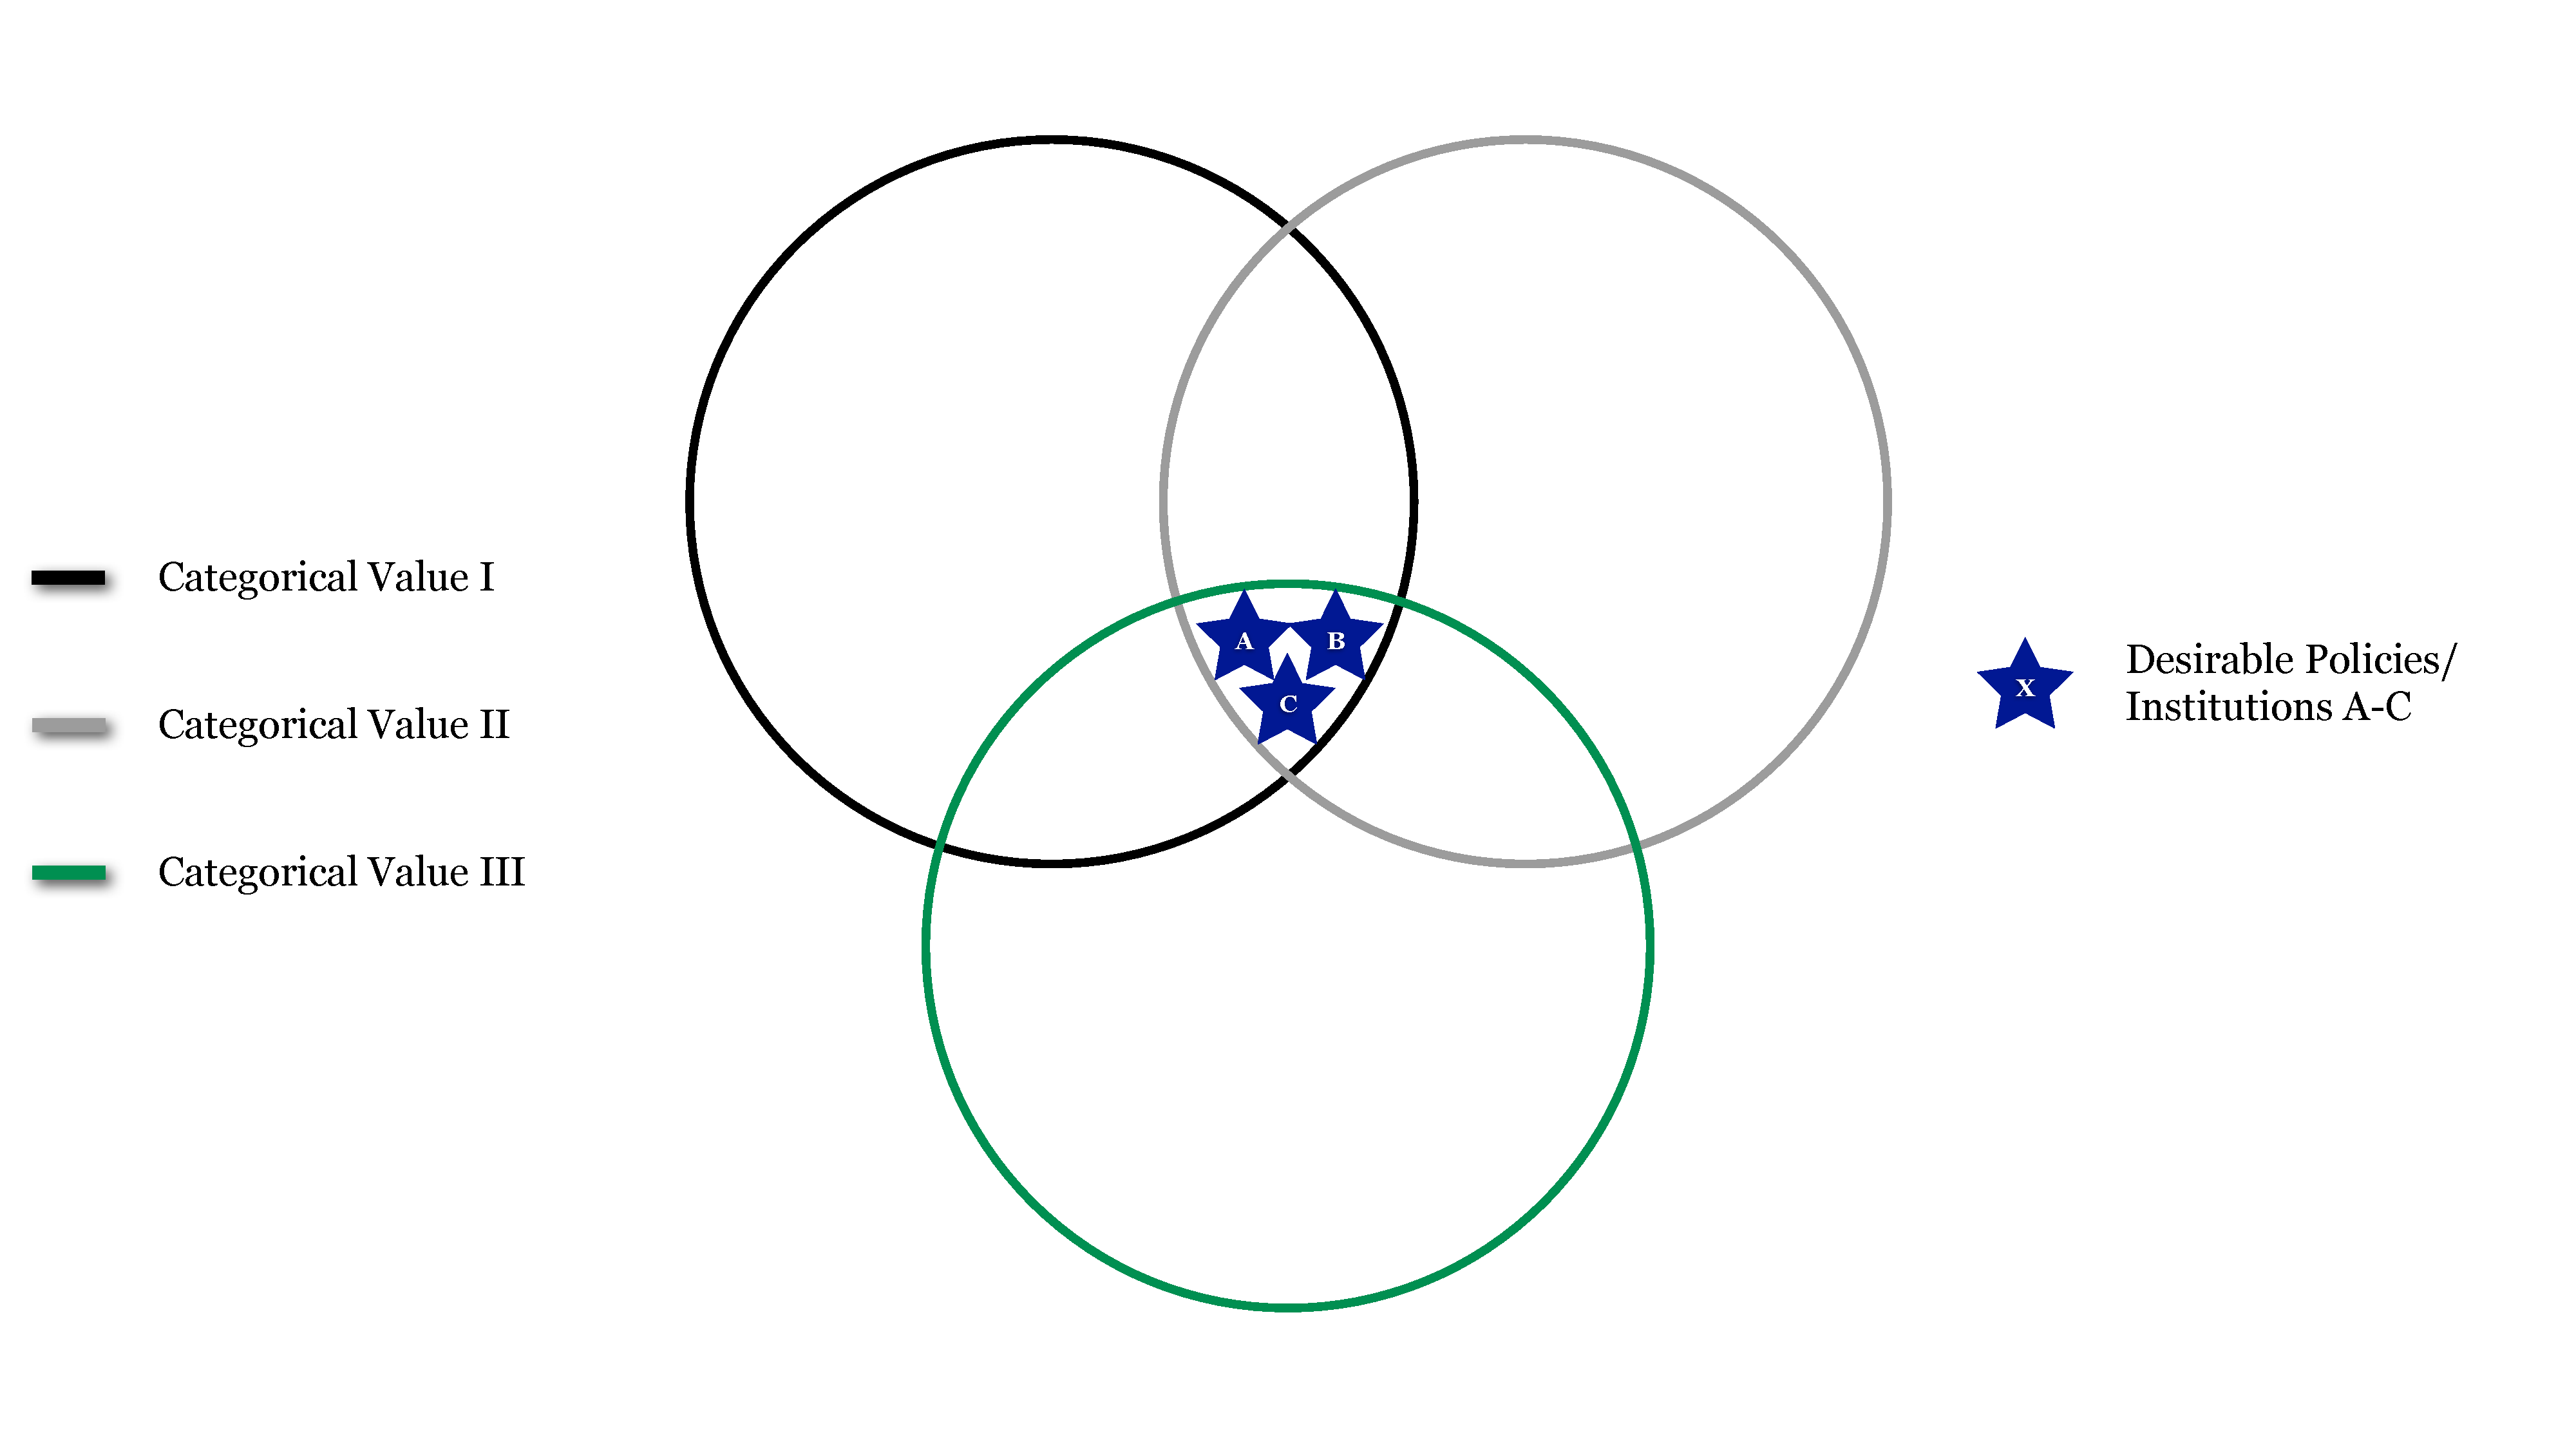
\includegraphics[width=1\textwidth]{euler-values}  
			\caption{Euler Diagram of Three Values}
			\label{fig:euler-values}
		\end{figure}

		All remaining values must be reconciled within this intersect of categorical values of liberalism.
		Here too, even supposedly outsized cardinal gains in any of the remaining values cannot be traded off nominal violations of categorical values.
	\item
		In part, I resolve these conflicts by offering trade-offs.
		This works only for values that are continuous in their realization, as may be the case for the tired conflict between equity and efficiency in taxation. %add href
		I suggest that the trade-offs offered by such conflicting, continuous values depend crucially on the institutional context under which these trade-offs have to be engaged.
		Calling trade-offs, and designing the conditions thereof can be illustrated well in a diagram of \glspl{PPF}, frequently used in economics to illustrate different possible baskets of goods that can be produced by an economy. 
		Because paper as this is two-dimensional, \gls{PPF} diagrams frequently only show two goods, but the abstraction carries to any number of $n$ goods in a basket.
		I adapt the traditional \gls{PPF} in \autoref{fig:ppf-values} (p.~\pageref{fig:ppf-values}). 
\end{enumerate}

\begin{figure}[htbp]
	\centering
	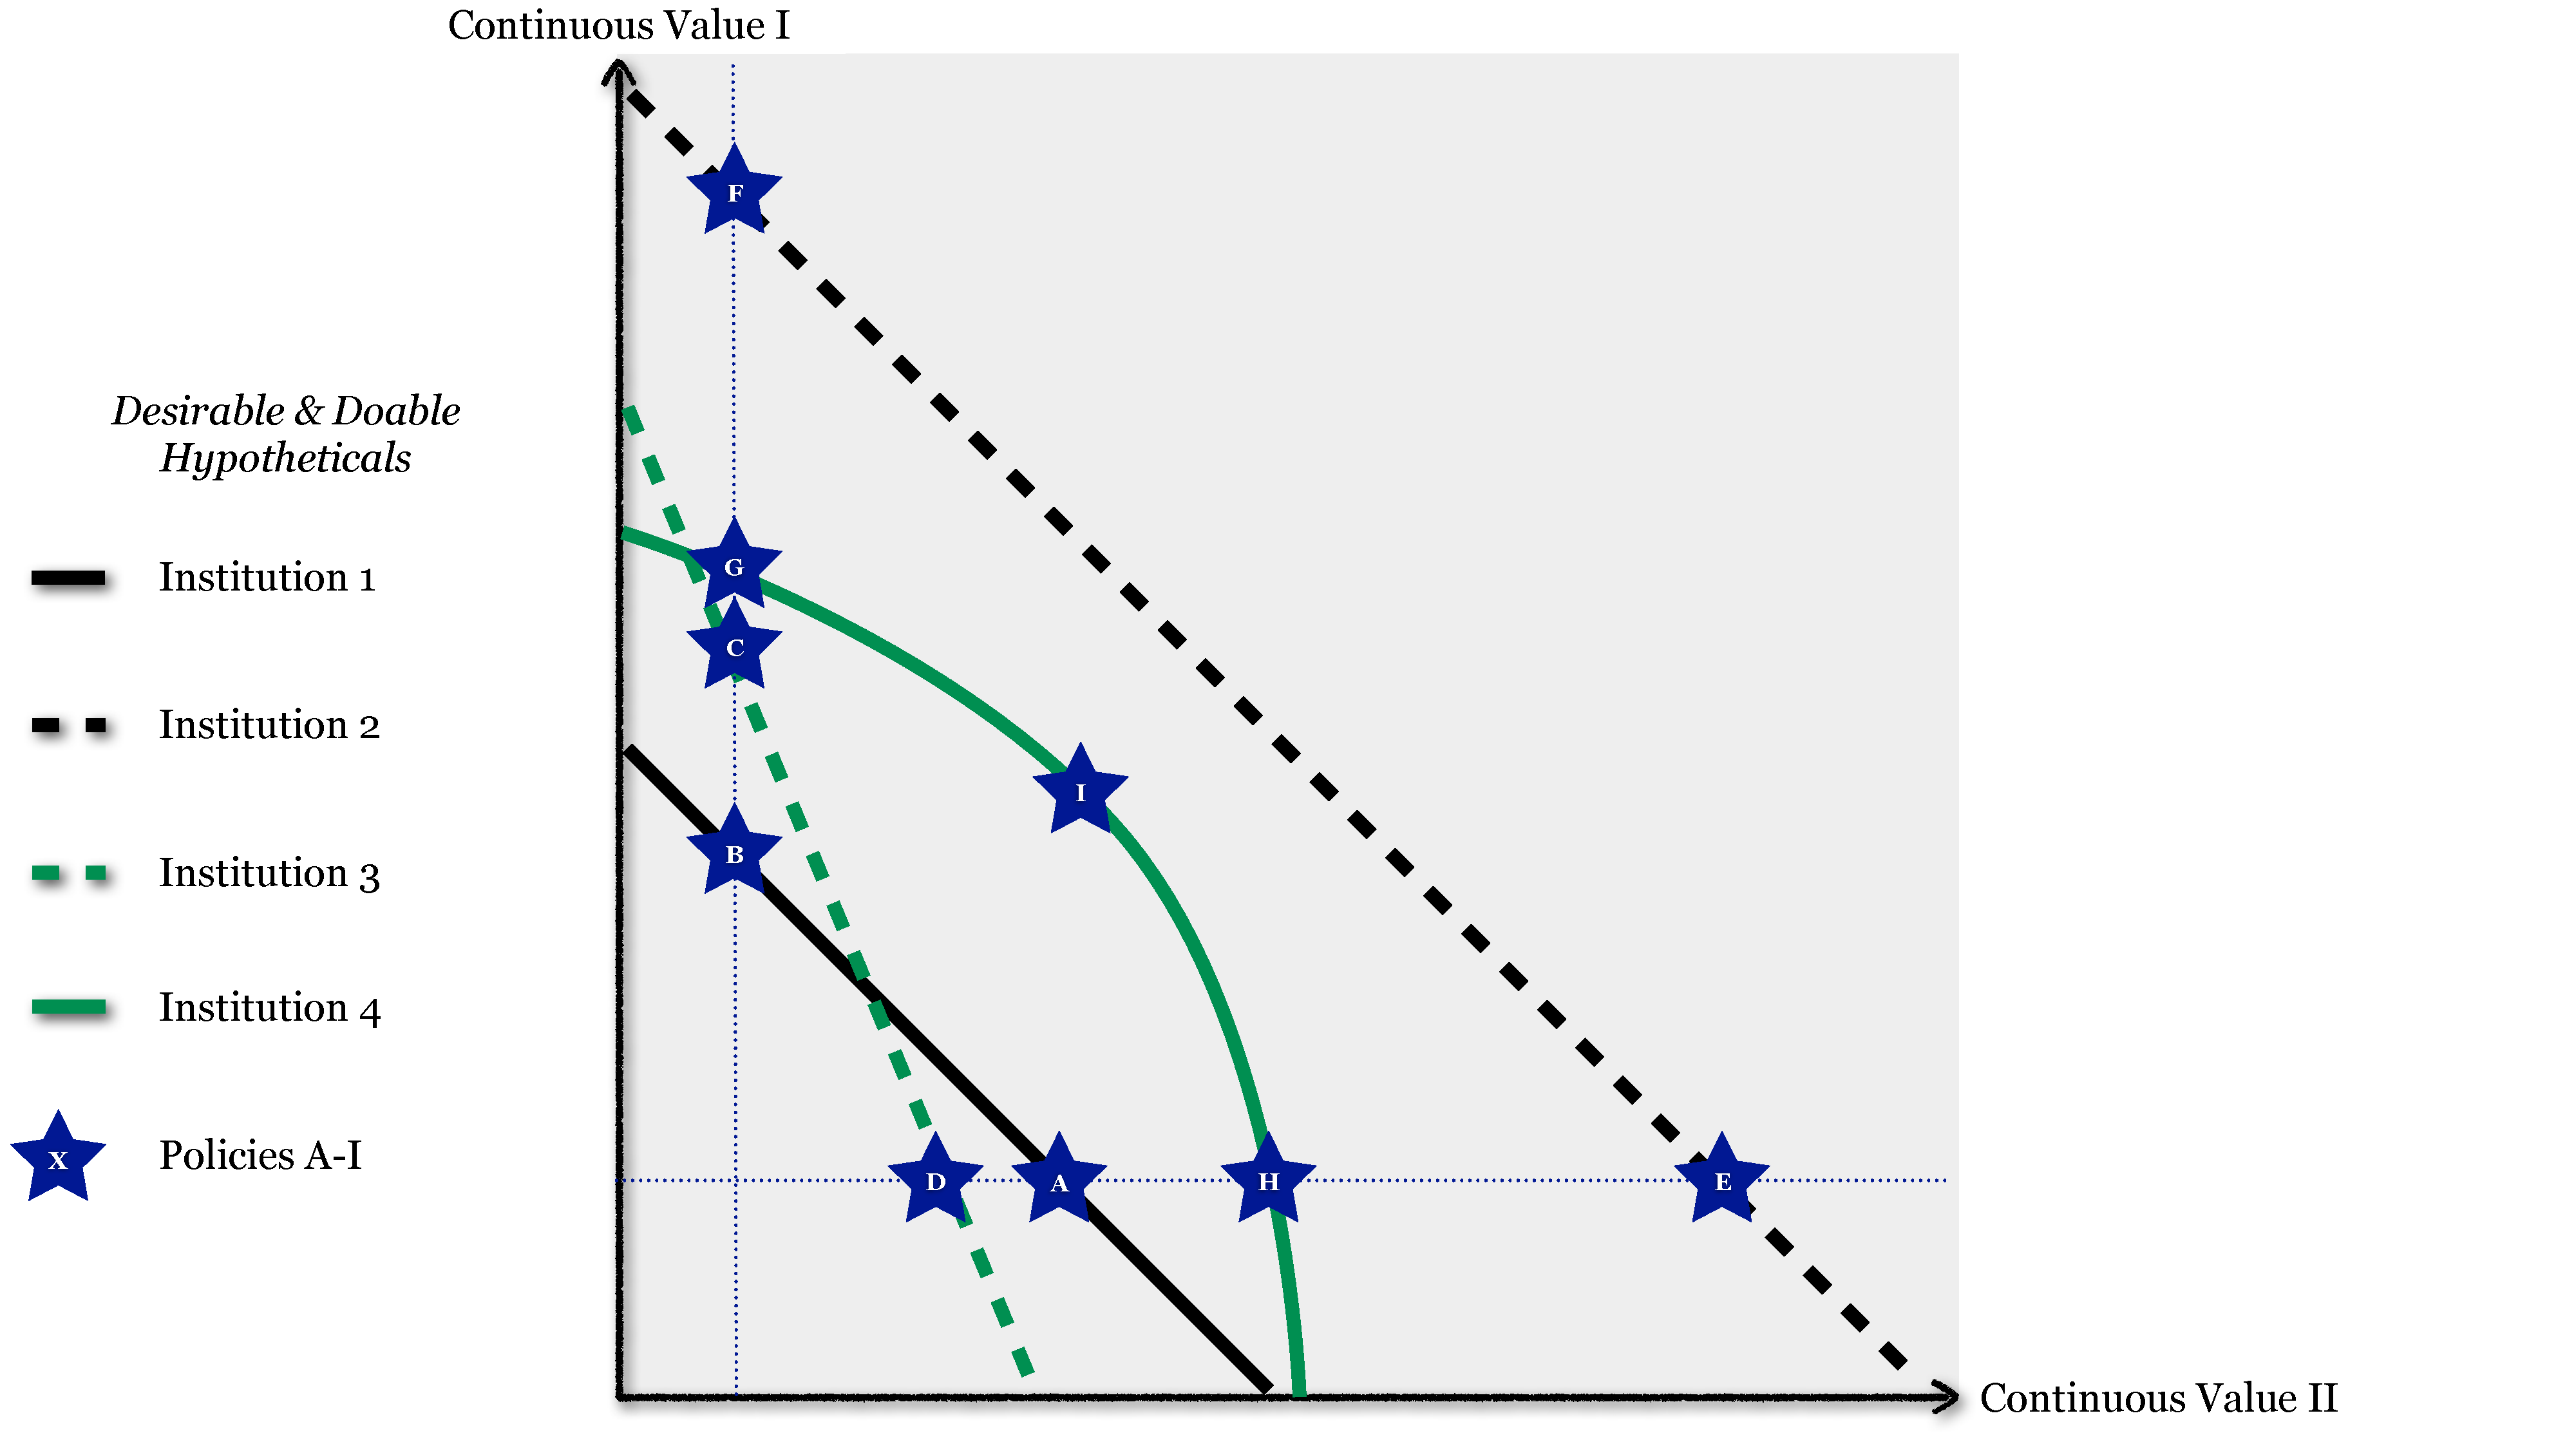
\includegraphics[width=1\textwidth]{ppf-values}  
	\caption{Production-Possibility Frontiers of Two Competing Values}
	\label{fig:ppf-values}
\end{figure}%economies of scale variant is still missing

	What are competing goods in a \gls{PPF} diagram are here competing values $I$ and $II$. 
	Let us assume for the sake of simplicity that these values can be easily measured and are ratio scaled.
	More of each value is better.
	The four \glspl{PPF} are comprised of those possible combinations of values $I$ and $II$ which are \emph{furthest} from the origin, and thereby strictly preferable over all possible policies \emph{under} the \gls{PPF}.
	As in a static model of the economy, the \glspl{PPF} are exogenously determined by a priori, and posteriori limits of the first order.
	In addition, I argue, these exogenous limits are modified by \emph{institutions} $1$ through $4$.
	 Policies $A$ through $J$ are defined by specific combinations of continuous value $1$ and $2$, along the respective institutions which modify what is logically and empirically possible in this world.
	
	\autoref{fig:ppf-values} illustrates different policy choices.
	The simplest kind of trade-off is that between two policies along a linear \gls{PPF}, as between $A$ and $B$ on $1$.
	A straight \gls{PPF} implies that the values are substituted at a constant rate: any increase in $I$ will requires a decrease in $II$ by the same amount.
	The choice between $A$ and $B$, as all other points on $1$ is a zero-sum proposition.
	As we shall see, trade-offs in welfare, taxation and democracy are frequently, if implicitly, presented as such zero-sum choices.
	Alternatives of this sort are inevitable, but they are also normatively less interesting.
	Once values $I$ and $II$ are reduced to the same scale, the choice along the resultant \gls{PPF} becomes trivial or even arbitrary
	\footnote{
		In the technical terms of introductory economics, individual preferences are expressed in \emph{indifference curves}, that is, the lines along those combinations of $I$ and $II$ between which a person is indifferent.
		The intersection between the aggregate of these indifference curves would be the optimal policy point(s). %is this true?
		If the aggregate indifference curve is curvilinear and reasonably simple, there will be one or few such points.
		If, however, the aggregate indifference curve is \emph{linear} and scaled as the \gls{PPF}, \emph{all} policies along the \gls{PPF} intersect with an identical indifference curve, and there are an infinite number of ideal policy points.
		%I think here's a big question: are indifference curves curvilinear or linear? and why? How is this related to scaling?
	}.%add refs to later misunderstandings here
	
	\gls{PPF} $4$ is curvilinear, and more interesting. 
	Here, the rate of substitution varies over different levels of $I$ or $II$.
	For example, around $G$, you have to give up relatively little in $I$ to gain relatively much in $II$. 
	The reverse is true around $H$, and substitution is roughly constant around $J$.
	The trade-offs between $I$ and $II$ are non-zero-sum: you can gain more than you loose.
	Assuming a reasonable aggregate indifference curve (linear or convex), optimal policy will probably lie around $J$.
	As we shall see, concave or other curvilinear \glspl{PPF} abound in welfare, tax and democracy.
	Recognizing the convexity of trade-offs offered by any given institution, or, if possible, moving from lower, linear \gls{PPF} $1$ to a higher, convex \gls{PPF} $4$ will be important to identify desirable hypotheticals.%add later hrefs
	
	\glspl{PPF} $1$ and $3$ are both linear, but they have different slopes. 
	At any level of $I$, compared to \gls{PPF} $1$ you have to sacrifice more in $I$ to increase $II$.
	The moves \emph{along} curve $3$ are otherwise as normatively uninteresting as those along \gls{PPF} $1$ --- the two are just scaled differently --- but the choice \emph{between} these two institutions will be very consequential.
	Compared to institution $1$, institution $3$ will always make it costlier to increase value $II$.
	There are many such consequential choices of institutions in tax, welfare and democracy. %add hrefs
	
	\glspl{PPF} $1$ and $2$ both have the same slope, but $2$ is further from the origin.
	By definition, all policies along this higher curve are preferable to all policies on the lower curve --- to everyone
	\footnote{
		Technically, again, \emph{no matter the indifference curve}, the higher, but equally-sloped \gls{PPF} will always be preferable. 
	}
	.
	This is the most important of institutional choices to be made.
	
		%hehe, here's a pretty big part of the story missing: the DEMAND side. You'd need indifference curves!

%note how justice as fairness falls in-between these ... it's somewhere in-between all of those

%why is this pragmatic?

\section[Ontology]{The Ontology of The Doable Hypothetical} \label{sec:ontology} 

\textsuperscript{\ref{fn:also-in-europe}}

%ontology is the stuff that I am dealing with

%``(\ldots) every research agenda must start from some basic assumption about human nature, and the assumption of my research agenda is that despite all the evil in the world, at least some humans have, some of the time, a sense of goodness in truly caring for the well-being of others.'' \cite[7]{Steiner2012}

\begin{quote}
	\emph{``But what is government itself, but the greatest of all reflections on human nature?''}\\
	--- James \citeauthor{Madison1788} (\citeyear{Madison1788}: 143)
\end{quote}

Doable hypotheticals are preferable to others because, in \citeauthor{Dahl-1989-aa}'s words, ``we must avoid comparing ideal oranges with actual apples'' \citeyearpar[84]{Dahl-1989-aa}. 

Deciding just what can, and cannot be done is hard. 
If asked as a positive first-order question, the answer is sometimes empirically unclear. 
If turned into a second-order question --- as the social sciences are prone to do --- the answer becomes politically contested. 
Both extremes do not serve us well:
\begin{enumerate}
	\item 
		When all inquiries into the social world are reduced to positive, first-order questions the social sciences effectively abolish themselves and make the status quo epistemologically endogenous, as in: \emph{social inequality is inevitable human nature, because if it were not, it would not be observed}, or ``the Laws of commerce are the laws of Nature, and therefore the laws of God.'' (\citeauthor{Burke1790} as cited in \citealt[834]{Marx-1867-aa}).%find better source
	\item 
	Conversely, when such inquiries assign all positive questions to second-order status, the social sciences hermetically seal themselves off from other disciplines and turn critique into futile, infinite regress, as in: \emph{``social being [...] determines [...] consciousness''} \citep[Preface]{Marx1859}, including, one might add, Marxist consciousness. %find out that one piece that argues that social scientists are leftist because they get paid by the state 
\end{enumerate}

Instead, the social sciences --- and especially policy analysis --- should find a middle ground, taking on \emph{one second-order question at a time}, while provisionally leaving all other questions to first-order status. 

I here ask second-order questions about the welfare state, taxation and democracy and I therefore assume these \emph{institutions} to be malleable. 
\emph{Not} under study here are \hyperref[sec:human-nature]{human nature} (p.~\pageref{sec:human-nature}) or the \hyperref[sec:modernity]{modern condition} (p.~\pageref{sec:modernity}), especially of developed states and late capitalist economic production. 
I assume these to be constant in the medium run and reasonably approximated in the following sections.

\subsection[Human Nature]{Human Nature} \label{sec:human-nature}
Any second-order prescription for how to organize production, distribution and decision making rests on assumptions about human nature. 
For evolutionary anthropology, psychology, behavioral economics and other offspring of now disreputable \citep{Wright1994} sociobiology \citep{Wilson1975} this is a positive first-order question about our prehistoric baggage: what behavioral, cognitive and emotional dispositions might have been adaptive in the environment of our evolution, and what do we observe today?

\subsubsection[Evolution and Morality]{Evolution and Morality} 
Maybe, evolution deserves to be the master ontology of life, and therefore, of human life, too.
Because I sometimes refer to such Neo-Darwinian arguments \citep{Wright1994} and hear them often misunderstood I must reiterate the ontological status of the theory of evolution:

\begin{enumerate}
	\item 
		Evolution may dispose us to think, feel and act in certain ways, but does not determine us to do so (\emph{deterministic fallacy}).
	\item	
		Evolution yields more (``gradual'' according to Neo-Darwinism) or less (``punctuated'' according \citealt{Elrdredge1972}) stable \emph{equilibria} between environmental conditions and (more or less) adaptive traits of organisms. 
		It does not necessarily yield \emph{optimal} configurations, just survival of the relatively fitt\emph{er}. 
		Conversely, not all biological features that are observed are necessarily adaptive, but may simply be side consequences of other, adaptive features or developmental vestiges \citep{Gould}. 
	
	Or, in \citeauthor{Bryson2003}'s succinct formulation, ``life wants to be, but it doesn't want to be much'' \citep{Bryson2003}.
	
	\item \label{itm:nonmoral} 
		Evolution is a ``nonmoral'' process \citep{Gould1982}. 
		It may tend towards greater complexity and cooperation, including human-like intelligence \citep{Wright2000}, or it may just pursue a random walk, departing from a ``left wall'' \citep[4]{Gould1994} of ``simple beginnings'' \citep[7]{Gould1977}, and inevitably bring some complexity, including \emph{homo sapiens} as a freak outlier \citep{Gould1996}. 
		Either way, even if evolution \emph{were} directional, it would not be along any moral dimension intelligible to humans. This cuts both ways: 
		\begin{enumerate}
			\item 
				to praise evolutionary results is to fall for a \emph{``naturalistic fallacy''} (\citealt{Moore1903}, as cited in \citealt[K5987]{Wright2000})
			\item 
				to criticize them on any moral basis is to commit a \emph{``moralistic fallacy''} \citep{Davis1978}.
		\end{enumerate}
\end{enumerate}

Within these ontological limits, evolution serves me well in this dissertation, because as a materialist, positive and first-order perspective it allows me to limit my second-order inquiries on taxation and democracy. %include examples!

Unfortunately, evolutionary logic has a way of straying beyond the positive, of encroaching on and negating normative questions, precisely because it purports to explain all life, including human life. 
For example, if exclusive fitness were operative in human evolution, does that not, as Social Darwinism suggested, imply that humans \emph{are} unequal, end of story? 
More fundamentally --- and less obviously ideological --- if all our flesh, including our brain tissue, evolved in an aimless process, does that not, as overzealous neuroscientists like to test, imply that whichever subjective experiences of consciousness and free will that flesh reports must be wholly illusory, and all questions of morality therefore beside the point? 
If we were merely organic, delusional robots, as \citet[Chapter 23]{Wright2000} provocatively asks, what would be wrong with unplugging a few?

This pedestrian thesis is not the place for another mind-body debate, and I am equally awed and outmatched by these and other ``hard problem(s) of consciousness''  \citep{Chalmers1995}. 
Still, I must ask the reader to allow me a crude bit of lay metaphysics. 

For starters, positive questions on consciousness --- including the downstream issue of free will --- easily run into seemingly obvious logical problems. 
If consciousness were positively illusory, who would be left to do the observing? 
Conversely, if consciousness were some positive emergent neuronal phenomenon, would not precisely that physical genesis negate subjective experience? 
Either way, infinite regress ensues. Perhaps, as James \citeauthor{Trefil1997} muses, consciousness ``is the only major question in the sciences that we don't even know how to ask'' \citeyearpar[15]{Trefil1997} and maybe, therefore, we need not be bothered, for now.

More fundamentally, whatever we may learn about the (aptly named) ``neural \emph{correlates} of consciousness'' (for example, \citealt{Koch2004}, emphasis added) none of this positive research can, or ever should negate, or infringe on normative questions. 
The first-order positive questions of natural science, and the first-order normative questions of the social sciences should be kept neatly apart, because they are \gls{NOMA} \citep{Gould1997}. 
Akin to science and religion, first-order positive and normative questions, too are distinct ``domain(s) where one form of teaching holds the appropriate tools for meaningful discourse and resolution'' \citep[3]{Gould2002}: 
\begin{quote}
	\emph{``The magisterium of science covers the empirical realm: what the Universe is made of (fact) and why does it work in this way (theory). The magisterium of religion extends over questions of ultimate meaning and moral value. These two magisteria do not overlap, nor do they encompass all inquiry (consider, for example, the magisterium of art and the meaning of beauty).''}\\*
	--- Steven Jay \citet[6]{Gould2002} %add first name
\end{quote} 

No matter then, how hard-nosed a question we may ask about our evolved nature, these positive inquires must never be mistaken for, or negate normative questions, because these fall into categorically different realms:
\begin{quote}
	\emph{``Our failure to discern a universal good does not record any lack of insight or ingenuity, but merely demonstrates that nature contains no moral messages framed in human terms. 
	Morality is a subject for philosophers, theologians, students of the humanities, indeed for all thinking people. 
	The answers will not be read passively from nature; they do not, and cannot, arise from the data of science. 
	The factual state of the world does not teach us how we, with our powers for good and evil, should alter or preserve it in the most ethical manner.''}\\*
	--- Stephen Jay \citet[43]{Gould1982}
\end{quote}

\emph{Ought may imply can} \citep[65]{Kant1794}, but they are still not the same thing. 
However much constricted positive science may find us to be, these limits of what we \emph{can} do must never drown out the imperative \emph{ought}. 
Perhaps, tautologically, to be human and not another animal, is to arrogantly insist that, in spite of the limited and banal flesh we are made off, we \emph{ought} to be conscious, we \emph{ought} to have free will and we \emph{ought} to say ``ought''. 

Maybe, this is the this-wordly obedience to Jesus Christ that Dietrich Bonhoeffer meant --- and died for --- when, faced with fascism he chose ``costly discipleship'' \citep{Bonhoeffer1937}: ``Only he who shouts for the jews is permitted to sing Gregorian chants'' (Bonhoeffer 1933 as cited and translated in \citealt[35]{DeGruchy1999}). 
Fascism, after all, was the modern ideology to radically negate any ``ought'' for whichever group (``race''!) was supposedly biologically superior, and de-facto militarily stronger.
Perhaps, such rejection of ``ought'', too, makes the ``banality of evil'' that Hannah \cite{Arendt1963} recognized in an Adolf Eichmann on the stand in Jerusalem. 
Eichmann, after all, might ``excuse[...] himself on the ground that he acted not as a man but as a mere functionary [...] since after all, someone had to do it'' \citep[K286f.]{Arendt1963}. 
Such \emph{acts of state} defy \emph{ought}, because, to an ``unthinking'' Eichmann \citep[K187f.]{Arendt1963}, history --- as evolution --- just \emph{is}.

Such lay metaphysics might be crude, but they are \emph{not} entirely beside the point of welfare, taxation and democracy. 
As I argue later, a milder, but similar conflation of \emph{can} and \emph{ought}, of second-order positive, and first- and second-order normative questions plagues some social science, especially when it \hyperref[chap:hypotheticals-matter]{lacks hypotheticals} (\autoref{chap:hypotheticals-matter}, p.~\pageref{chap:hypotheticals-matter}). 
In the social sciences, too, the line between an emerged, evolved, ``grown order'' and a ``made order'' is sometimes blurred, negating political \emph{oughts} --- and not always as elegantly and explicitly as by \cite[37]{Hayek1973}.

\subsubsection{Evolution and Institutions}
We need not confine evolutionary explanations to our biology alone, or, conversely, reduce all behavior, cognition and emotion to some strictly physical (genetic) reason. 
Instead, we can apply evolutionary explanations to \emph{culture} and \emph{institutions}, too. 

In fact, the tired --- and often unproductive --- nature vs. nurture controversy is moot: we are neither blank slate
\footnote{
	\ldots \emph{aka.} \emph{tabula rasa} or \emph{homo sociologicus}, as \cite{Dahrendorf1965} quipped.
} 
for behaviorism to condition or society to write on, nor a physically determined animal, but essentially \emph{both} nature and nurture. 
Our bodies and culture-ready brains genetically \emph{co-evolved} with co-adaptive memes \citep{Dawkins1976} to make us the ``hypercultural species'' that we are \citep[K175]{Henrich2007}. 
Relatively ill-equipped in instincts, we need to \emph{learn} (or \emph{imitate}) what to eat and hunt --- and how to build a blast furnace. 
Perplexingly, it is in our \emph{nature} to rely on \emph{culture}: as our brain allowed us to learn easily, our culture developed cooking, and our digestive tract adapted to broken-down proteins, as illustrated in \autoref{fig:coevolution-nature-culture} (p.~\pageref{fig:coevolution-nature-culture}, \citealt[confer][]{Henrich2007}).

\begin{figure}[htbp]
	\begin{center}
	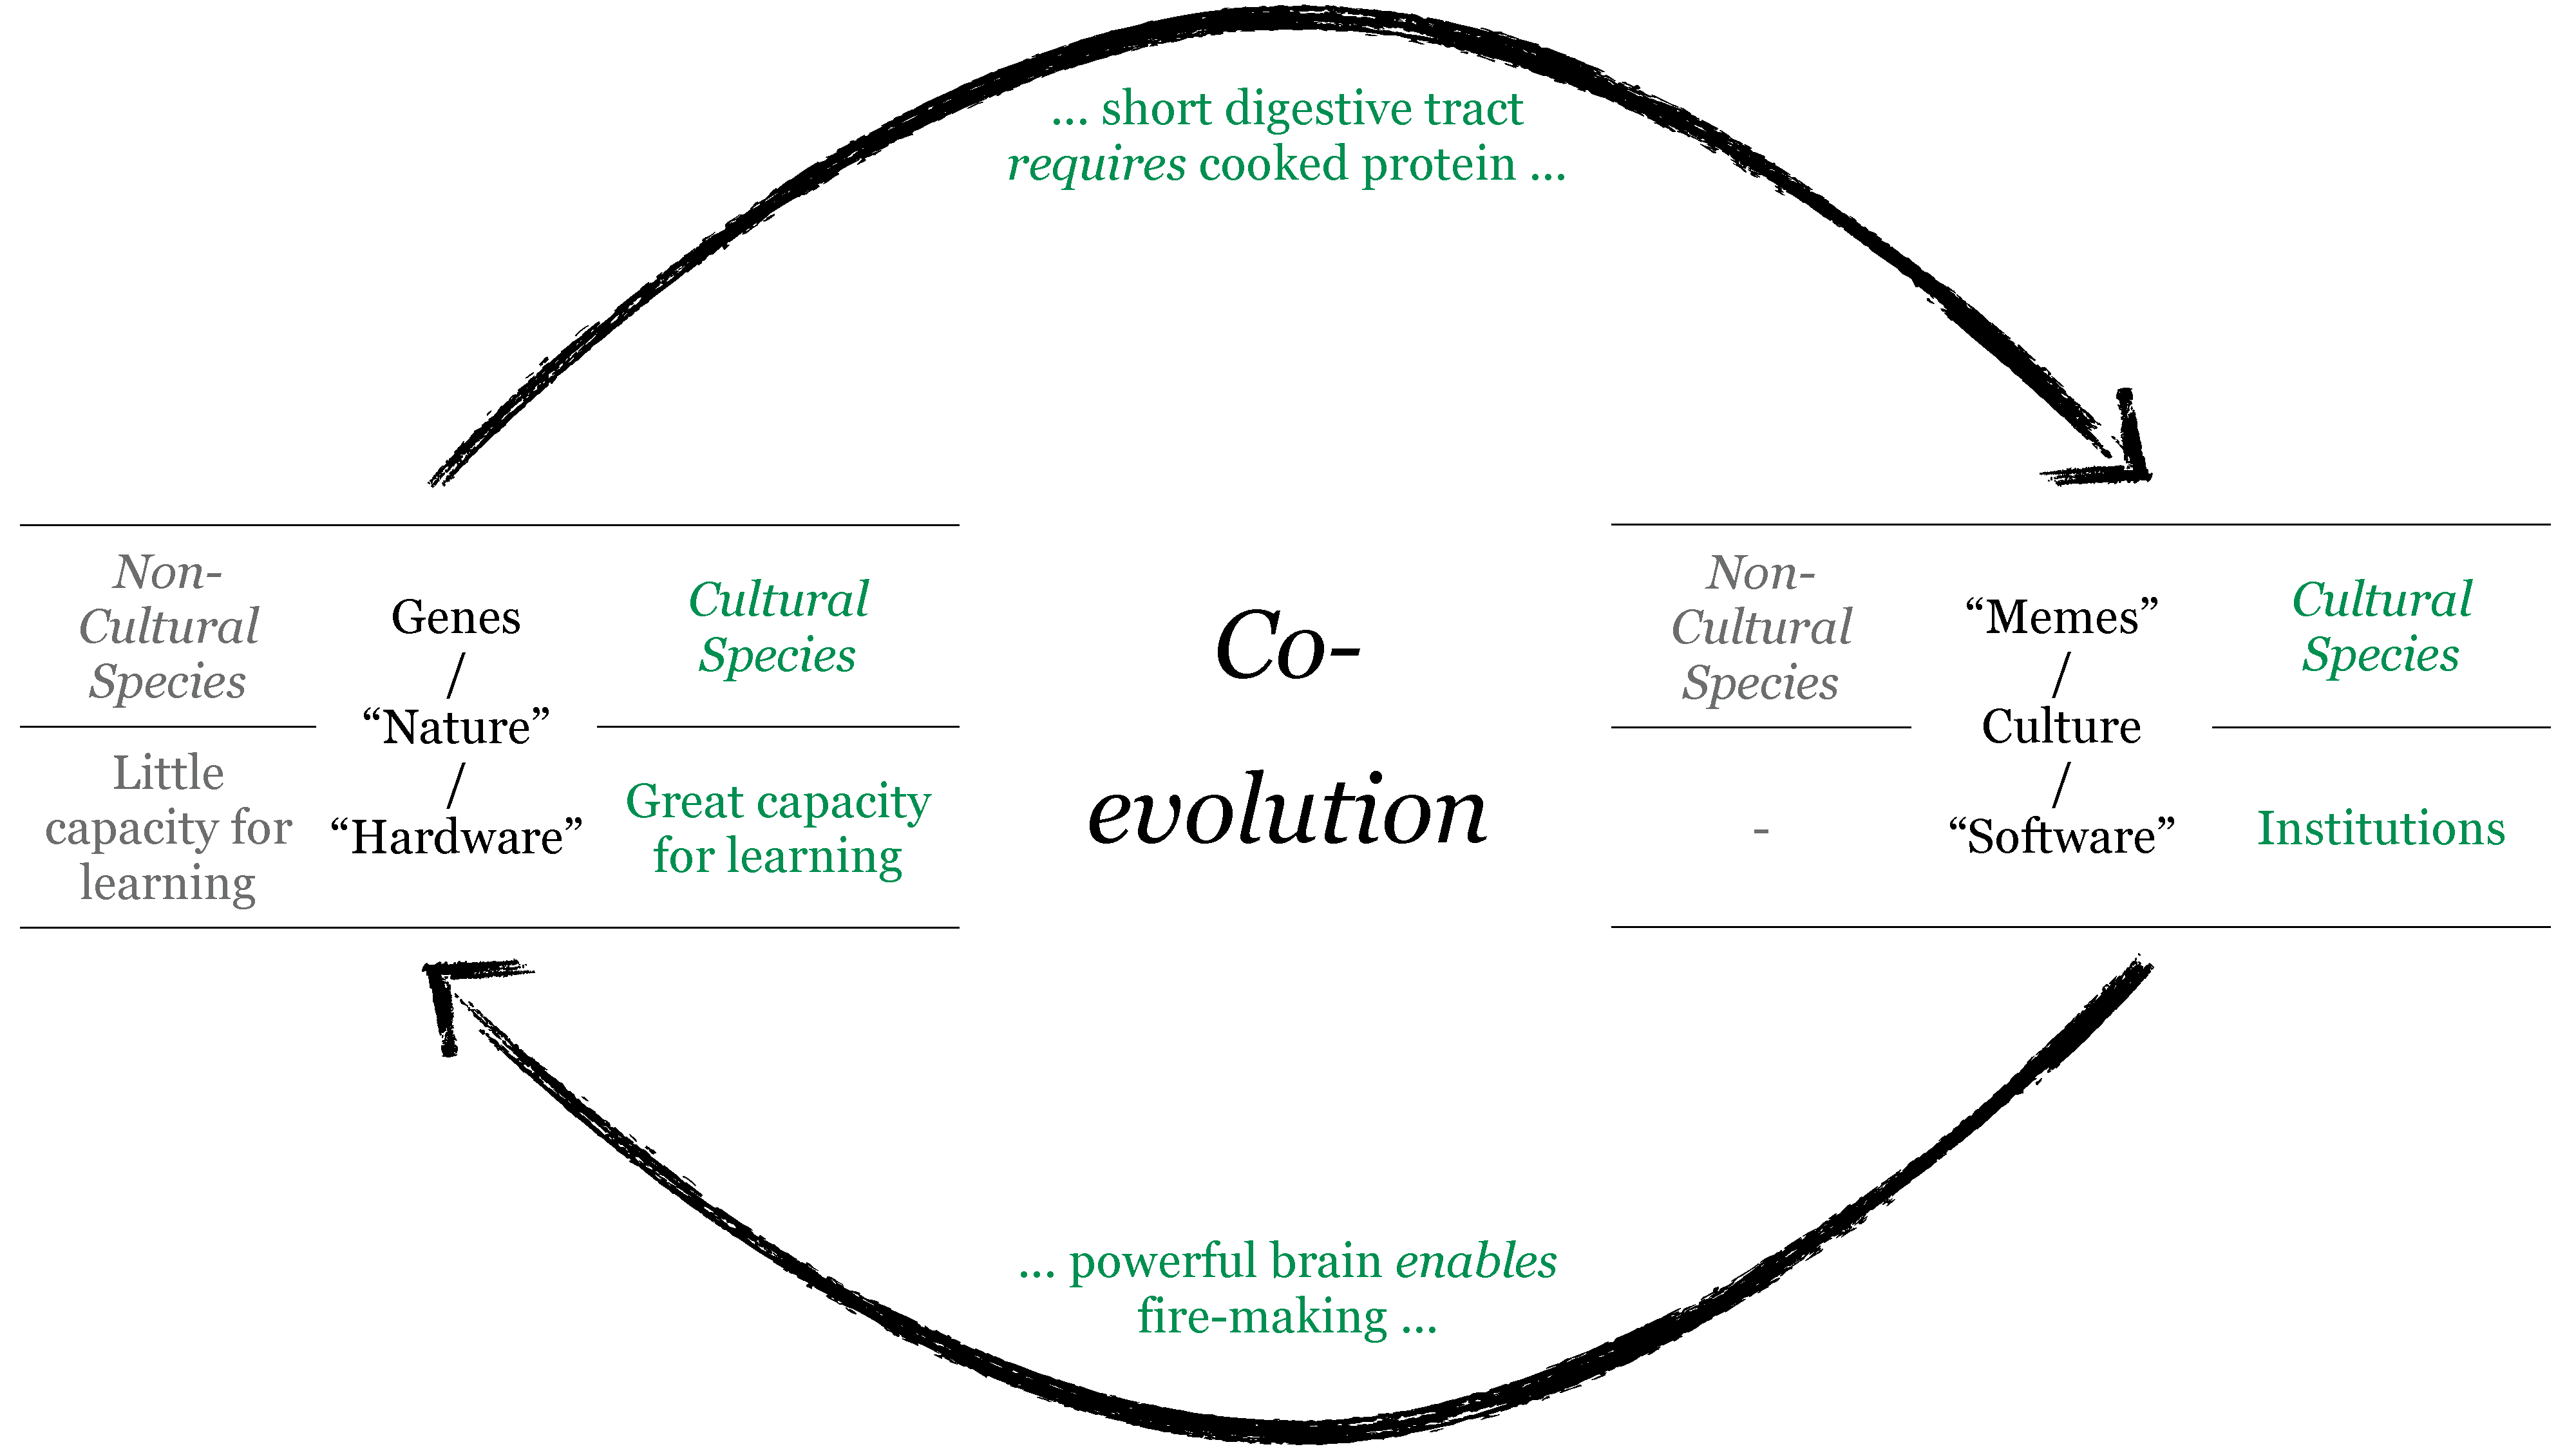
\includegraphics[width=1\textwidth]{coevolution-nature-culture}  
	\caption[Coevolution of Nature and Culture]{The coevolution of nature and culture, with some examples}	
	\end{center}
	\scriptsize{Own illustration, based on \citet[K120ff]{Henrich2007}}
	\label{fig:coevolution-nature-culture}
\end{figure}

This is the evolutionary blockbuster of humans: we moved the locus of our evolutionary adaptation from genes to memes \citep{Dawkins1976}. 
Instead of ``hard-coding'' all adaptive traits, we learn (or imitate) the more complex and more malleable software of culture (\citealt{Boyd1985}, \citealt[K196ff]{Henrich2007}), written not in \gls{DNA}, but coagulated into institutions. 

Paradoxically, as the naturally hypercultural species, we might gain some leeway from our biology, but simultaneously loose it to culture, because evolved culture too, must be (co-)adaptive to our biology, environment and, crucially, our \emph{past}, path dependent culture (\emph{evolutionary anthropology}, for example, \citealt{Wright2000}). 
As sociologists like to say about institutions --- the coagulates of culture --- culture, too, may \emph{enable us as it constrains us} (for example, \citealt{Hodgson2006}: 3). 

Here lurks another positive first-order dead end: if present culture is, by definition, sufficiently (co-)adaptive to persist, does that not imply that any new, improved culture could and \emph{would} emerge by said evolutionary process if, \emph{and only if}, it were (co-)adaptive to our nature and environment and sufficiently incremental from past culture? 
If, therefore, culture and institutions, too, were strictly positive phenomena unamenable to human will, would the social sciences and political critique not be completely beside the point? %cite Neiman somewhere in here? for example, http://www.fortschrittsforum.de/debattieren/bildung-modernisierung/artikel/article/bequemlichkeit-ist-was-fuer-realisten.html#tx-comments-comments-163

Hardly so. 
Here, as in all evolutionary arguments, the \emph{can} need not, and must not eclipse the \emph{ought}. 
We may not be able to make arbitrary institutions, but, axiomatically, we \emph{can} build \emph{progressive} institutions: they help us achieve normative ends, by first responding to our evolved cultural and natural dispositions, then transcending them. 
At least since Enlightenment dawned, we get to make our own history (a little), and build or break (some) institutions as an act of will --- that is \hyperref[itm:pragmatic-ethics]{ethical pragmatism} (p.~\pageref{itm:pragmatic-ethics}). 

To build institutions is to emancipate ourselves from the meaningless process that bore us as expendable containers of ``selfish genes'' \citep{Dawkins1976} and to heed that call for morality, that we among the earth's animals may hear clearest, because through institutions, we \emph{can} turn reflexive on our innate behavior, cognition and emotions. 

\subsection[Modernity]{The Modern Condition} \label{sec:modernity} 
Maybe this is as good a definition of modernity as any: the project by which we reflect on what might be innate to our existence and inevitable about our physical world, and deliberately build institutions accordingly. 
Thus advises a machiavellian \citeyearpar{Machiavelli1532} \citeauthor{Mandeville1714} to turn ``private vices by dextrous management of a skillful politician (\ldots) into public benefits'' \citeyearpar[213]{Mandeville1714}, thus threatens a somber \cite{Hobbes-1651-aa} our inner wolves with an even more powerful metaphorical beast, and thus asks us a moralizing \cite{Smith-1776-lq} to receive from others ``from their regard to their own interest'' --- or any number of other ``idea[s] of the world as open to transformation, by human intervention'' \citep[94]{Giddens1998}.

Modernity, as evolution, is often misused or misunderstood, and so again, I must briefly clarify its ontological status for my purposes:

\begin{enumerate}
	\item 
		The modern project need not be confined to a specific location or era, nor need it be one-directional or linear, but it might arise in different places at different times, it might wax and wane, explode and collapse. 
		While Europe and North America in the early 21st century may constitute high points in this project, the modern project is not wedded to any specific historical context or even the institutions which it bore, but rather, modernity is a \emph{cultural} and \emph{cognitive} phenomenon \citep[26, emphasis added]{JonesJones-2003-aa}.
	%include reference to diamond on the arbitrariness of why modernity happened in western europe
	\item 
		The modern project need not be inherently good nor necessarily lead to desirable outcomes: modernity may well bear alienation \citep{Adorno1966}, or even lead to catastrophe \citep{Bauman1989} and not all of its (ongoing) advances may yield progress. 
	
		However, the inverse is true: to think progress implies a modern mindset, and to get it done requires modern institutions.

	\item 
		It should be redundant to say that my dissertation ontologically assumes a modern condition, because tautologically, sociology is about finding answers to the questions modernity raises \citep[325]{Harriss2000}, and ``postmodern sociology [therefore] an impossibility'' \citep[169]{Miles-2001-aa}. 
	
	And yet, ``modernity'' seems to be a concept fallen out of fashion, superseded by (occasionally loose) talk of various post-isms (for example, \citealt{Lyotard1984}, Baudrillard) or second and reflexive modernities \citep[for example,][]{BeckBonss-2003-aa}.
	
	Whatever the value of these and other contributions, in welfare, taxation and democracy I find no contradictions that would require such categorical labels or the nascent theories they stand for. 
	In fact, I suspect that a thoroughly \emph{modern} analysis of welfare, taxation and democracy may resolve many of those contradictions which reflexive modernity prematurely identifies, and clarify some of the uncertainties in which postmodernity revels. 
	For instance, maybe, equipped with a rational and deep understanding of the mixed economy and externalities, we find that ``de-nationalization'' \citep{BeckGrande-2007-aa} and ``risk society'' \cite{Beck-1992-aa} are neither inevitable, nor particularly descriptive but simply avoidable and unsurprising cooperation problems, instead. %add \href
	
	I here reflect on many dysfunctions of the presently observed, undoubtedly modern institutions of welfare, taxation and democracy, but I need not get ``all meta'' about modernity, because precisely such ``reflexivity is a modern, not postmodern set of attitudes and practices and that ritualized postmodern caviling against modernity is ahistorical and inaccurate, not to mention dispiriting'' \citep[1119]{Sica-1997-aa}. 
	
	Also, as I promised earlier, this \emph{is} a pedestrian thesis.
\end{enumerate}

What then, are these indispensable modern institutions that I here assume as ontological entities, that which defines the ``doable''? 

\subsubsection{States and Markets}
For the production and distribution of goods, they are state plan (but not \emph{nation state}) and market exchange (but not any particular x-\emph{capitalism}). 
For collective decision making, they are a state equipped with an effective monopoly on the use of force and devoted to some popular participation \citep[compare][96]{Giddens1998}.

These two, states and markets, both \emph{brought} and \emph{constitute} the modern condition: they hyper-charged functional differentiation \citep{Smith-1776-lq} to reach near-planetary breadth (for example, international trade, citizenship) and near-universal depth (for example, commodification, family law), they altered or replaced much of the evolved culture (for example, kin) and institutions (for example, tribe) adaptively fit only at smaller scale \citep{Diamond1997}, replaced such mechanical by organic solidarity \citep{Durkheim-1893-aa} and bore a social world that is complexly interacting \citep[for example,][]{Merton-1968-aa,Merton-1936-aa}. 

These two are also the meta-institutions that both define and allow welfare, taxation and democracy. 
Welfare and taxation exist only, as I explain later, in mixed economies of both market exchange and state plan. 
Taxation and democracy alike, to become real, must be enforced by a state with an effective monopoly on the use of force.%add \href
	
As all modern institutions, state and market are based on a particular model of human nature, in this case, a
\begin{enumerate}
	\item rational and %also included in the axioms
	\item individual 
	\item utility-maximizing %also included in the axioms
\end{enumerate}
\emph{homo economicus} \citep[maybe first in][]{Mill1848}. 
The state gets an amoral, but opportunistic \emph{homini lupus} to behave by threatening monopolistic force \citep[as in][]{Hobbes-1651-aa}. 
The market, in turn, lures a self-seeking, but rational ``butcher, [...] brewer, or [...] baker'' into providing ``our dinner'' --- and all else --- ``from their regard to their own interest'' \citep{Smith-1776-lq}. 

\subsubsection[Nonzero]{Non-Zero-Sumness \label{sec:nonzero}}
But, as other modern institutions, state and market not only assume this human nature, they also allow homo economicus to transcend her own limits. 
As \emph{individual} utility-maximizers, she runs into problems whenever her supposed selfishness prevents otherwise mutually advantageous interactions. 
This rough typology specifies the class of games which homo economicus is ill-equipped to solve:

\begin{enumerate}
	\item 
		\emph{Zero-sum} games display constant sums of payoffs over all cells, or possible interactions. 
		One player's gains equal another player's losses: the cake does not grow, but is only sliced up differently. 
		By definition, a zero-sum game is pareto optimal: no one can be made better off, without making someone else worse off
		\footnote{
			Critics of economic growth (but not \gls{GDP}!) should carefully ponder the implications of such a scenario: a world with no economic growth is a world where \emph{all} human interactions are zero-sum. 
			Empirical literature on, for example, rentier economies, have chronicled the corrupting influence that zero-sumness may have on a political process, when all decisions create \emph{nothing but} winners and losers \citep{Beblawi1990}.
		}.
	
		Terms of trade, the ratio of units of goods that a country has to export for any unit of imports, is an oft-cited (rare) example of zero-sumness in advanced economies.%add citation
	
		A trivial example of zero-sumness, theft, (without spillovers) is illustrated in \autoref{tab:theft}: all cells yield the same $\sum{\text{payoffs}}=2$.
	
	\item 
		\emph{Non-zero-sum} games have different sums of payoffs, or possible interactions. 
		One players gains are not equal to another players losses: the cake can grow or shrink. Positive-sum games are equivalent to negative-sum games, because the absence of a loss (a negative-sum outcome) is a gain (a positive-sum outcome). 
		For the sake of simplicity, I often refer to only gains or positive-sum outcomes, but mean all non-zero-sum games. 
		Crucially, non-zero-sumness does not imply that gains are shared equally, or at all. Non-zero-sum games need not even imply (weak) pareto-improvements, if one players looses less than another gains in a Kaldor-Hicks-improvement \citep{Kaldor1939,Hicks1939}.
	
	Non-zero-sum games further break down into:
	\begin{enumerate}
		\item 
			\emph{Games of total harmony} are situations in which self-interested players will \citeauthor{Nash1951}-equilibrate at an interaction that reaps all non-zero-sumness
			\footnote{
				\emph{Strategies}, or players' moves, form a \emph{Nash equilibrium} if they are mutually \emph{best responses}. 
				Best responses, in turn, are the utility-maximizing move for a player, \emph{given} the other player's choice. \emph{Dominant strategies} are those best responses that maximize payoffs over \emph{all} choices of the other player(s). 
				The \emph{social welfare optimum} is realized under those combinations of strategies that maximize the aggregate payoffs of all players. 
				\cite{Kleinberg-2009-oz} provide a great introduction into game theory and its basic concepts.
			}.
			By definition, a game of total harmony offers pareto improvements: at least one player \emph{can} be made better off, (at least) without making someone else worse off.
		
			Under some assumptions, opening up to free trade famously is such a game of total harmony \citep{Ricardo1817}. 
			It is roughly illustrated in \autoref{tab:trade}: at $\sum{\text{payoffs}}=6$, the north-western cell yields the highest, social optimum and it is also the only (!) set of mutually best responses, and thereby, the unique Nash equilibrium. 
			In short: trade and other games of perfect harmony should take care of themselves.
		
		\item 
			\emph{Cooperation problems} plague non-zero-sum situations where the social welfare optimum is not also (at least) \emph{a} Nash equilibrium. 
			Here, at least one player may gain more than all others stand to loose. %is this true?
			Such games cannot be Pareto-, but only Kaldor-Hicks improved.
		
			The canonical example of a cooperation problem, a \gls{PD}, is given in \autoref{tab:PD}: here the socially optimal (smallest) payoff $\sum{\text{payoffs}}=2$ prison years its in the north-western cell, but it does not constitute a mutually best response. 
			In fact, no matter what the other player does, one is always better off betraying: the south-eastern cell is not only a mutually best response and thereby the Nash equilibrium, but even a mutually \emph{dominant} strategy at a dismal aggregate prison sentence of $\sum{\text{payoffs}}=6$ years.
		
			The \gls{PD} and related cooperation problems can model many of the economic and political challenges facing us today, including global warming \citep[for example,][]{Stern-2006-aa} and herding in financial markets (from \citealt {Keynes1936} to \citealt{Banerjee-1992-aa}). 
			I also identify \gls{PD}-style problems in welfare, taxation and democracy. %add \hrefs
	\end{enumerate}
\end{enumerate}

\begin{table}
	\caption[The Theft Game]{Theft as a Zero-Sum Game}
	\label{tab:theft}
	\begin{center}
	\begin{tabular}
		{m{1cm}
		m{2,3cm}
		m{2,3cm}
		m{2,3cm}
		m{2,3cm}}
	
		
 %empty cell
& %empty cell 
& \multicolumn{2}{c}{\emph{Player A}} 
\\


 %empty cell
& %empty cell 
&Does not steal 
&Steals
\\ 

\cline{3-4}

\multicolumn{1}{c}{\multirow{4}{*}{\emph{Player B}}} 
& \multirow{2}{2,3cm}{Does not steal} 
& 	\multicolumn{1}{|r|}{1} 
& \multicolumn{1}{r|}{2}
\\ 


\multicolumn{1}{c}{} 
& \multicolumn{1}{c}{}
& \multicolumn{1}{|l|}{1} 
& \multicolumn{1}{l|}{0}
\\ 

\cline{3-4}

\multicolumn{1}{c}{} 
& \multirow{2}{2,3cm}{Steals} 
& \multicolumn{1}{|r|}{0} 
& \multicolumn{1}{r|}{1}
\\ 


\multicolumn{1}{c}{} 
& \multicolumn{1}{c}{}
& \multicolumn{1}{|l|}{2} 
& \multicolumn{1}{l|}{1}
\\ 

\cline{3-4}

\end{tabular}
\end{center}

	\scriptsize{
		Player A and Player B both have a good. 
		They can steal from each other, or not steal. 
		By heroic assumption, theft has no interaction costs and does not erode trust or security.
		
		Payoffs are units of enjoyment of goods. 
		Higher is better. 
		As always, cardinal numbers are examples, only ordinal relations matter.}
\end{table}


\begin{table}
	\caption[The Trade Game]{Ricardian Trade as a Game of Perfect Harmony}
	\label{tab:trade}
	\begin{center}
	\begin{tabular}
		{m{1cm}
		m{2,3cm}
		m{2,3cm}
		m{2,3cm}
		m{2,3cm}}

%empty cell
&
& \multicolumn{2}{c}{\emph{Home}} 
\\


%empty cell
& 
&Trade 
&Autarky
\\ 

\cline{3-4}

\multicolumn{1}{c}{\multirow{4}{*}{\emph{Rest of the World}}} 
& \multirow{2}{2,3cm}{Trade} 
& 		\multicolumn{1}{|r|}{2} 
& \multicolumn{1}{r|}{1}
\\ 


\multicolumn{1}{c}{} 
& \multicolumn{1}{c}{}
& \multicolumn{1}{|l|}{4} 
& \multicolumn{1}{l|}{3}
\\ 

\cline{3-4}

\multicolumn{1}{c}{} 
& \multirow{2}{2,3cm}{Autarky} 
& \multicolumn{1}{|r|}{1} 
& \multicolumn{1}{r|}{1}
\\ 


\multicolumn{1}{c}{} 
& \multicolumn{1}{c}{}
& \multicolumn{1}{|l|}{1}
& \multicolumn{1}{l|}{1}
\\ 

\cline{3-4}
\end{tabular}
\end{center}
	
\scriptsize{
	Home country and Rest of the World can decide to open up to trade or remain under autarky. 
	Because both countries have different opportunity costs, as per \citeauthor{Ricardo1817}'s theorem of comparative advantage, they both stand to gain from trade, if possibly unequally.
	
	Payoffs are the baskets of goods to be consumed. 
	Higher is better. 
	As always, cardinal numbers are examples, only ordinal relations matter.
	
	Trade cannot be adequately modeled in two-dimensional payoff-matrix with only two players because, trivially, if one player reverts to autarky, the other player must also choose autarky because there is no trading partner left. 
	I ignore that problem here by assuming that the rest of the world will always find some exogenous trading partner.
}
\end{table}

\begin{table}
	\caption[The Prisoners' Dilemma Game]{The Prisoners' Dilemma as a Cooperation Problem}
	\label{tab:PD}
	\begin{center}
	\begin{tabular}
		{m{1cm}
		m{2,3cm}
		m{2,3cm}
		m{2,3cm}
		m{2,3cm}}

%empty cell
& 
& \multicolumn{2}{c}{\emph{Prisoner A}} 
\\


%empty cell
& 
&Stays Silent 
& Betrays
\\ 

\cline{3-4}

\multicolumn{1}{c}{\multirow{4}{*}{\emph{Prisoner B}}} 
& \multirow{2}{2,3cm}{Stays Silent} 
& 	\multicolumn{1}{|r|}{1} 
& \multicolumn{1}{r|}{0}
\\ 


\multicolumn{1}{c}{} 
& \multicolumn{1}{c}{}
& \multicolumn{1}{|l|}{1} 
& \multicolumn{1}{l|}{2}
\\ 

\cline{3-4}

\multicolumn{1}{c}{} 
& \multirow{2}{2,3cm}{Betrays} 
& \multicolumn{1}{|r|}{2} 
& \multicolumn{1}{r|}{3}
\\ 


\multicolumn{1}{c}{} 
& \multicolumn{1}{c}{}
& \multicolumn{1}{|l|}{0} 
& \multicolumn{1}{l|}{3}
\\ 

\cline{3-4}
\end{tabular}
\end{center}
\scriptsize{
	Prisoner A and Prisoner B are both arrested, but police has insufficient information for a conviction. 
	The two are separated, and police offers both independently the same leniency deal: if one betrays the other, she will go free, and the other prisoner goes to jail for 2 years. 
	If both betray one another, they will both go to jail for 3 years. If they both stay silent, they will only be charged with a minor crime and get 1 year in jail.
	
	Payoffs are years in jail. 
	Lower is better. 
	As always, cardinal numbers are examples, only ordinal relations matter.}
\end{table}

If we are to reap the (great) benefits of non-zero-sumness, homo economicus must be able to successfully play these classes of games. 
She should do well in games of perfect harmony that cater to her selfish utility maximization, but might flounder cooperation problems. 
As a maximizer of \emph{individual} utility, she cannot see the bigger picture of aggregate welfare.

Such is, for example, the logic of a \citeauthor{Hobbes-1651-aa}ian war of everyone against everyone: all would be better off if they ceased fighting, but in a world where everyone is armed and angry, any individual homo economicus better not be a pacifist. 
In fact, security may be modeled as a \gls{PD}, as in \autoref{tab:PD-security}. 

\begin{table}
	\caption{Security as a Prisoners' Dilemma}
	\label{tab:PD-security}
	\begin{center}
	\begin{tabular}
		{m{1cm}
		m{2,3cm}
		m{2,3cm}
		m{2,3cm}
		m{2,3cm}}
	
%empty cell
& 
& \multicolumn{2}{c}{\emph{Homo homini \ldots}}
\\


%empty cell
& 
&\ldots ovis 
& \ldots lupus
\\\\ %why more slashes?

\cline{3-4}


\multicolumn{1}{c}{\multirow{4}{*}{\emph{Homo homini \ldots}}} 
& \multirow{2}{2,3cm}{\ldots ovis} 
& 	\multicolumn{1}{|r|}{2} 
& \multicolumn{1}{r|}{3}
\\ 


\multicolumn{1}{c}{} 
& \multicolumn{1}{c}{}
& \multicolumn{1}{|l|}{2} 
& \multicolumn{1}{l|}{0}
\\ 

\cline{3-4}

\multicolumn{1}{c}{} 
& \multirow{2}{2,3cm}{\ldots lupus} 
& \multicolumn{1}{|r|}{0} 
& \multicolumn{1}{r|}{1}
\\ 


\multicolumn{1}{c}{} 
& \multicolumn{1}{c}{}
& \multicolumn{1}{|l|}{3} 
& \multicolumn{1}{l|}{1}
\\ 

\cline{3-4}
\end{tabular}
\end{center}
\scriptsize{
	Two homo sapiens are both living in a \citeauthor{Hobbes-1651-aa}ian primordial state of war. 
	They can either be peaceful \emph{obis} (latin: sheep), or violent \emph{lupus} (latin: wolves) to their fellow men. 
	To be violent is costly, but promises a meal of sheep-like humans, or at least their resources (food, shelter). 
	If you are eaten, or, more benignly, robbed of food and shelter as a peaceful sheep, you receive no payoff, because either way, you must die or starve. 
	If two wolves meet, both engage in costly violence but receive no extra resources.
	
	Payoffs are utility, as in food or shelter. 
	Higher is better. 
	As always, cardinal numbers are examples, only ordinal relations matter.}
\end{table}

In a more realistic model with many players instead of just two, the cooperation problem may only exacerbate. 
If you were the only wolf amongst many sheep, violence may be especially cheap, because your potential victims are plenty and helpless. 
Conversely, being a lone sheep amongst many wolves will be especially risky for the sheep, and costly for the wolves who need to be competitively violent. 
At such a larger scale, the \gls{PD} of security evolves into an arms race with ever costlier, but fruitless violence: the original tragedy of the commons \citep{Hardin-1968-aa}.

Naturally ``stuck in-between'' \citep{Lehrer2012} the selfishness of homo economicus and our capacity for altruism
\footnote{
	Altruistic behavior, according to \cite{Wilson2012} and before him \cite{Darwin1859}, is an emergent property of the \emph{group}, following group selection. 
	According to mainstream sociobiology \citep[and initially][]{Wilson1975}, altruism emerges at the \emph{individual} level by a strategy of inclusive fitness or genetic nepotism, helping others as they are related.
},
as ever the ``hypercultural species'' \citep[K175]{Henrich2007}, cooperative exploitation of non-zero-sumness, as much else, does not come to us robotically, or by instinct as it does to the eusocial insects \citep{Wilson2012}. 
In humans, such cooperation is \emph{contingent} on culture or institutions.

\subsubsection{The Genesis of Cooperation}
Luckily for us, history listened to \citeauthor{Hobbes-1651-aa} and brought such an institution for large-scale cooperation, when it bore those powerful \emph{Leviathans}, whom we have since successfully trained into rule-of-law, and even democratic states. 

Two theories of the genesis of states are instructive here:
\begin{enumerate}
	\item 
		Maybe, states are simply the largest remaining of pre-historic, atomistic racketeers who threatened \emph{with} well as \emph{protected from} violence \citep[182]{Tilly-1985-aa}. 
		These initially small-scale racketeers morphed into proto-states and then states as new technology, and --- equivalently --- economies of scale allowed them to produce and distribute violence at a larger scale, for lower cost \citep{Tilly-1985-aa}.
	\item 
		Or maybe, (nation!) states grew out of kinship ties and our capacity for genetic nepotism \citep{Hamilton1964,Axelrod1981a}, as the initially real blood lines became ever thinner and eventually illusory and fake, yet effective \citep{Van-den-Berghe-1981-aa,Gellner-1983-aa}. 
\end{enumerate}

The two stories need not be mutually exclusive, but may instead complement one another. 
After all, \citeauthor{Tilly-1985-aa}'s materialist account of state genesis does not so much explain away the cooperation problem, but reverts it to the level of individual thugs who make up the racketeering mafia. 
As Coppola's ``Godfather'' (1972, 1974, 1990) trilogy illustrates, even in the 20th century, successful organized crime is not easy, and hinges on trust. 
Anecdotally, in the case of the Corleone organization, cooperation is built on family ties, alluding to theories of inclusive fitness as nepotism. 
Maybe, economies of scale and first genetic, later imagined nepotism \emph{both} drove state making, only at different levels. %note that this matters for the later argument on property! Take this up somewhere!

Against this backdrop, the development of governance in the modern era, including sequentially security, the rule of law, democracy and welfare \citep[compare][]{Marshall-1950-aa} is a project of \emph{both} consolidating, and steering a powerful but dangerous monopoly on violence or illusion of kinship, respectively. 
Absent such training, states are quite scary beasts, as \citeauthor{Hobbes-1651-aa}'s frontispiece of \emph{The Leviathan} illustrates. 
Both theories of their genesis imply a slippery slope. 
Supercharged by economies of scale in the production of violence, those monopoly producers of violence may tend towards parasitic government. 
``Imagined communities'' \citep{Anderson-1983-aa}, in turn, enabling cooperation by increasingly fabricated nepotistic sentiment, may always risk turning exclusive, or even fascist if the quasi-biological notions run loose. 

Here again, the modern age has borne deliberate (meta?-)meta-institutions to govern an evolved structure, including constitutions, rule of law and democracy. 
However, all these modern additions to statehood should not distract from its defining innovation: an effective monopoly on the use of force, without which we are back to a very, very dismal square one. 
``You cannot get to Jefferson and Madison without going through Thomas Hobbes'' --- in Iraq \citep{Diamond-2004-aa}, or elsewhere. %page number missing

Modern markets, and the intricate games of perfect harmony they provide for homo economicus to solve and thrive, too, depend on this monopoly of force. 
From property rights, to contract law and fiat money, commerce always rests on effective enforcement: to enter any such deals in the first place, you must believe that really, \emph{pacta sunt servanda}, that promises \emph{will} be kept --- or made to be kept, anyway. 

It is, in fact, this shadow of violence that enables markets in the first place, that allows us to \emph{transform} cooperation problems into games of perfect harmony, and thereby, to \emph{solve} them. 

States and markets are, the atomistic reading of \citeauthor{Hobbes-1651-aa} and \citeauthor{Smith-1776-lq} aside, a feat of great cooperation. 
Almost magically, they freed us off that \citeauthor{Malthus1798}ian curse, by which our geometric population growth must always outstrip our \emph{arithmetric} economic growth, and starve us
\footnote{
	\cite{Malthus1798} might have been correct only about some periods of human history, and anyway, was anachronistic in his time, when functional differentiation was already well under way.
}.
The modern escape from that iron law of population (or resources, or carbon, and so on) \emph{was}, \emph{is} and \emph{will} be to make economic growth above-linear, too: to reap non-zero-sumness, to functionally differentiate and to harvest economies of scale. 
If at different altitudes of abstraction, these all imply the same prescription: cooperation \emph{is} our one ticket out of hardship and subsistence (a notion to which I return in the \hyperref[sec:growth-solidarity]{later} in \autoref{sec:growth-solidarity}, p.~\pageref{sec:growth-solidarity}).

\subsection{Contingent Homo Economicus} \label{sec:contingent-homo-economicus} 
To think about welfare, taxation and democracy, then, homo economicus is both inescapable and inadequate. 

\subsubsection{Inescapable Homo Economicus} 
As an ontological model, homo economicus is inescapable, because it comes part and parcel with the meta-institutions of state and markets. 
To think of coercive power or supply and demand is to invoke an individual utility-maximizer. 
By extension, to ponder welfare, taxation and democracy, too, implies this view of human nature, for if we were neither \emph{individual} nor \emph{utility maximizers}, altruism, allocation and decision making would come to us automatically. 
Alas, it does not.

\paragraph{Materially Possible.} 
Moreover, market and state, along with their view of human nature are good ontologies for a second-order inquiry into welfare, tax and democracy because market and state, if nothing else, are materially possible under first-order theory. %add \href

Market and the state may not be the only materially possible means to organize cooperation, but they are the only (meta-)institutions that have demonstrably orchestrated large-scale production and distribution of many kinds of goods. 
They, and the {the \hyperref[sec:sources-of-wealth]{sources of wealth} (p.~\pageref{sec:sources-of-wealth}) they tap into are the \emph{only known} way to prosperity. 

For now, only states can solve commons problems \citep[for example,]{Hardin-1968-aa}, and only markets efficiently and credibly gather, process and signal dispersed information \citep{Hayek1931}. 
Other institutions to facilitate cooperation, such as kinship \citep{Van-den-Berghe-1981-aa,Hammond2006} or even the nuclear family (on which the conservative/continental welfare state still relies heavily, according to \citealt{Esping-Andersen-1990-aa}) and community \citep{Ostrom1990} are often narrow in scope and reach. 
Self-organizing scientists (for example, The Human Genome Project), programmers (for example, Linux OS) and web-users (for example, Wikipedia) have lately accomplished impressive achievements, but their mode of production seems to complement state and market, rather than replace it: scientists are often paid state salaries, free software runs on commercial hardware, and wikipedians need day jobs. 
These goods, incidentally, are also all common or public goods, the non-state production of which we are only just beginning to understand \citep{Ostrom1990}. 

Eventually, great hopes set in volunteerism, a communal ``governing the commons'' \citep{Ostrom1990} or some other alternative mode of production, distribution and decision-making may come to fruition. 
In the meantime, we must stick to at least a bit of state and market, the two meta-institutions which, empirically, have civilized whichever aspects of homo economicus we might positively harbor into the intricately complex interdependency of the modern world.

This interdependency is, as I have explained, the very \emph{condition} of our prosperity. Modernity and its riches, we can only hope, are here to stay \citep{Diamond-2005-aa} and any first-order ontology, must --- as states and markets do --- abide by its conditions. 
The modern economy is, and \emph{needs to be} so functionally differentiated that no subset of people can ever organize, let alone meet all their material needs in isolation. 
Only elegant abstractions, such as global price systems, can enable this feat of cooperation. 
Likewise, modern society is so complex that no large share of society can ever comprehend, let alone decide on all matters of the polity. 
Only some people, some of the time, can comprehend in some detail and decide on some matters. 
In modernity, autarky is regress
\footnote{
	Such regressive states of disorganization can still be observed in much of the developing world \citep[confer][]{Clark2007,Easterly-2006-aa}, war zones \citep[on the Iraq example,][]{Baker-IIIHamilton-2006-aa} or wherever else human culture has regressed back to or stalled in innate (kin-, clan-) modes of cooperation \citep[on the southern italian example,][]{PutnamLeonardi-1993-aa}
}.

Small-scale, intimate interactions, such as of the ancient polis or the prehistoric tribe will not, and should not return. 
Any ontology or policy that purports a return to such simpler times does not, as it might claim, provide an \emph{alternative} to state or market, but instead merely defines away the question which these meta-institutions \emph{have} answered and threatens to roll back modernity.

\paragraph{Logically Consistent.} 
Homo economicus and the meta-institutions it inspired also make for a good ontology for hypotheticals, because whatever its shortcomings, at least, we have a \emph{logically consistent understanding} of states and markets, and know something about how they work, and how they fail. 
If you assume some homo economicus in us, an appeasing Leviathan, and the pareto-improving qualities of free markets, are, in fact, logically consistent. 

These abstractions ride on a lot of (heroic) assumptions, but at least, they clarify our thinking and generate falsifiable hypothesis. 
That is more than can be said about suggested remedial institutions such as ``governance'', ``Big Society'' (Cameron 2011) or a philanthropic ``Third Sector'' \citep{Anheier2002}. 
These, as many other recent contenders of states and markets, are shrouded in impenetrable \hyperref[sec:newspeak]{Newspeak} (``problem solving'', ``community'' and ``giving back'', respectively) (p.~\pageref{sec:newspeak}), they lack a coherent (\emph{any?}) model of human nature, and give no account of their successes and failures. 

Civil society, in particular, is yet only negatively defined (it is \emph{not} the state, \emph{not} the market and \emph{not} the family), its mode of production (volunteerism?) is underspecified and its vaguely optimistic ignorance of structure and material interest border on (hegemonial?) ideology. 
Here, too, defining away the contradictions of modernity will not solve them, it will merely render the advocated institutions inaccessible to critique and improvement.

\subsubsection{Inadequate Homo Economicus} 
Yet, homo economicus is the kind of quasi-evolutionary concept that blurs theory and data, and easily eclipses \emph{ought} with \emph{is}. 
Less metaphysically, it is also plainly inadequate to investigate welfare, taxation and democracy because these projects, as states and markets, more generally, are, and always have been plagued by precisely these selfish demons of our nature.

\paragraph{Logically Incomplete.} 
Homo economicus is logically incomplete as a first-order ontology, because it cannot explain the initial nucleus of cooperation from which states and markets must have sprung.

The infinite regress of an ontology inhabited only by homo economicus is evident in the competing (or complementing) theories of state genesis referenced earlier.
\citeauthor{Tilly-1985-aa}'s (and similar) stories of state-making-as-organized-crime do not so much explain \emph{Leviathan}-level cooperation, as they merely relegate it to the level of nascent racketeers: just \emph{how} these thugs initially ganged up, we do not know.
\citeauthor{Van-den-Berghe-1981-aa}'s (and related) stories of polities-as-extended-kinship, likewise, do not so much explain \emph{Imagined Communities}, as they simply relegate it to a sociobiological explanation of reciprocal altruism: just \emph{how} reciprocal altruism emerged at a \emph{group} level, in an evolution of \emph{individual}-borne genes and memes, we do not know, and even sociobiology is unsure
\footnote{
	Altruistic behavior, according to \cite{Wilson2012} and before him \cite{Darwin1859}, is an emergent property of the \emph{group}, following group selection. 
	According to mainstream sociobiology (and initially \citealt{Wilson1975}), altruism emerges at the \emph{individual} level by a strategy of inclusive fitness or genetic nepotism, helping others as they are related.
}.

Whatever their genesis, states, markets and modernity may well \emph{need} such nuclei of cooperation to sustain themselves, even today. 
In fact, much of their current crises might be described as the inevitable wreckage of pure homo economicus. 

This dissertation, too, chronicles the limits of homo economicus as much as it ontologically rests on this view of human nature.

\paragraph{Empirically Incomplete.} 
Luckily for us, this rational, individual utility-maximizing model of human nature may also be incomplete --- but not entirely incorrect --- on all counts: humans may be hard-wired altruists \citep[for example,][]{Zak2004}, are only boundedly rational \citep{Simon-1999-aa,Kahneman2011}, poor planners of utility \citep[summarized in][]{Gilbert2006}, think in relative, not absolute terms \citep{Frank2005} and display diminishing marginal utility \citep{Ng-1997-aa,Veenhoven-2000-aa,Nickell2008}. %check these references with the abote stuff on utility

Homo economicus provides, in other words, at least an \emph{incomplete} description of human nature.

\paragraph{Domain-Specific Homo Economicus.} 
Nevertheless, and because homo economicus is both inescapable and inadequate to investigate welfare, taxation and democracy, we should make this model of human nature and its related (meta-)institutions \emph{domain specific}.

Even if, as I suspect, there are no alternatives to state or market in \emph{some} realms of modern society, we need not ``economicize'', commodify or regulate \emph{all} aspects of life. 
Instead, different tasks call for different modes of production, distribution, decision making and associated views of human nature, as summarized in \autoref{tab:modes-human-nature}.

\begin{table}[htbp]
	\centering
	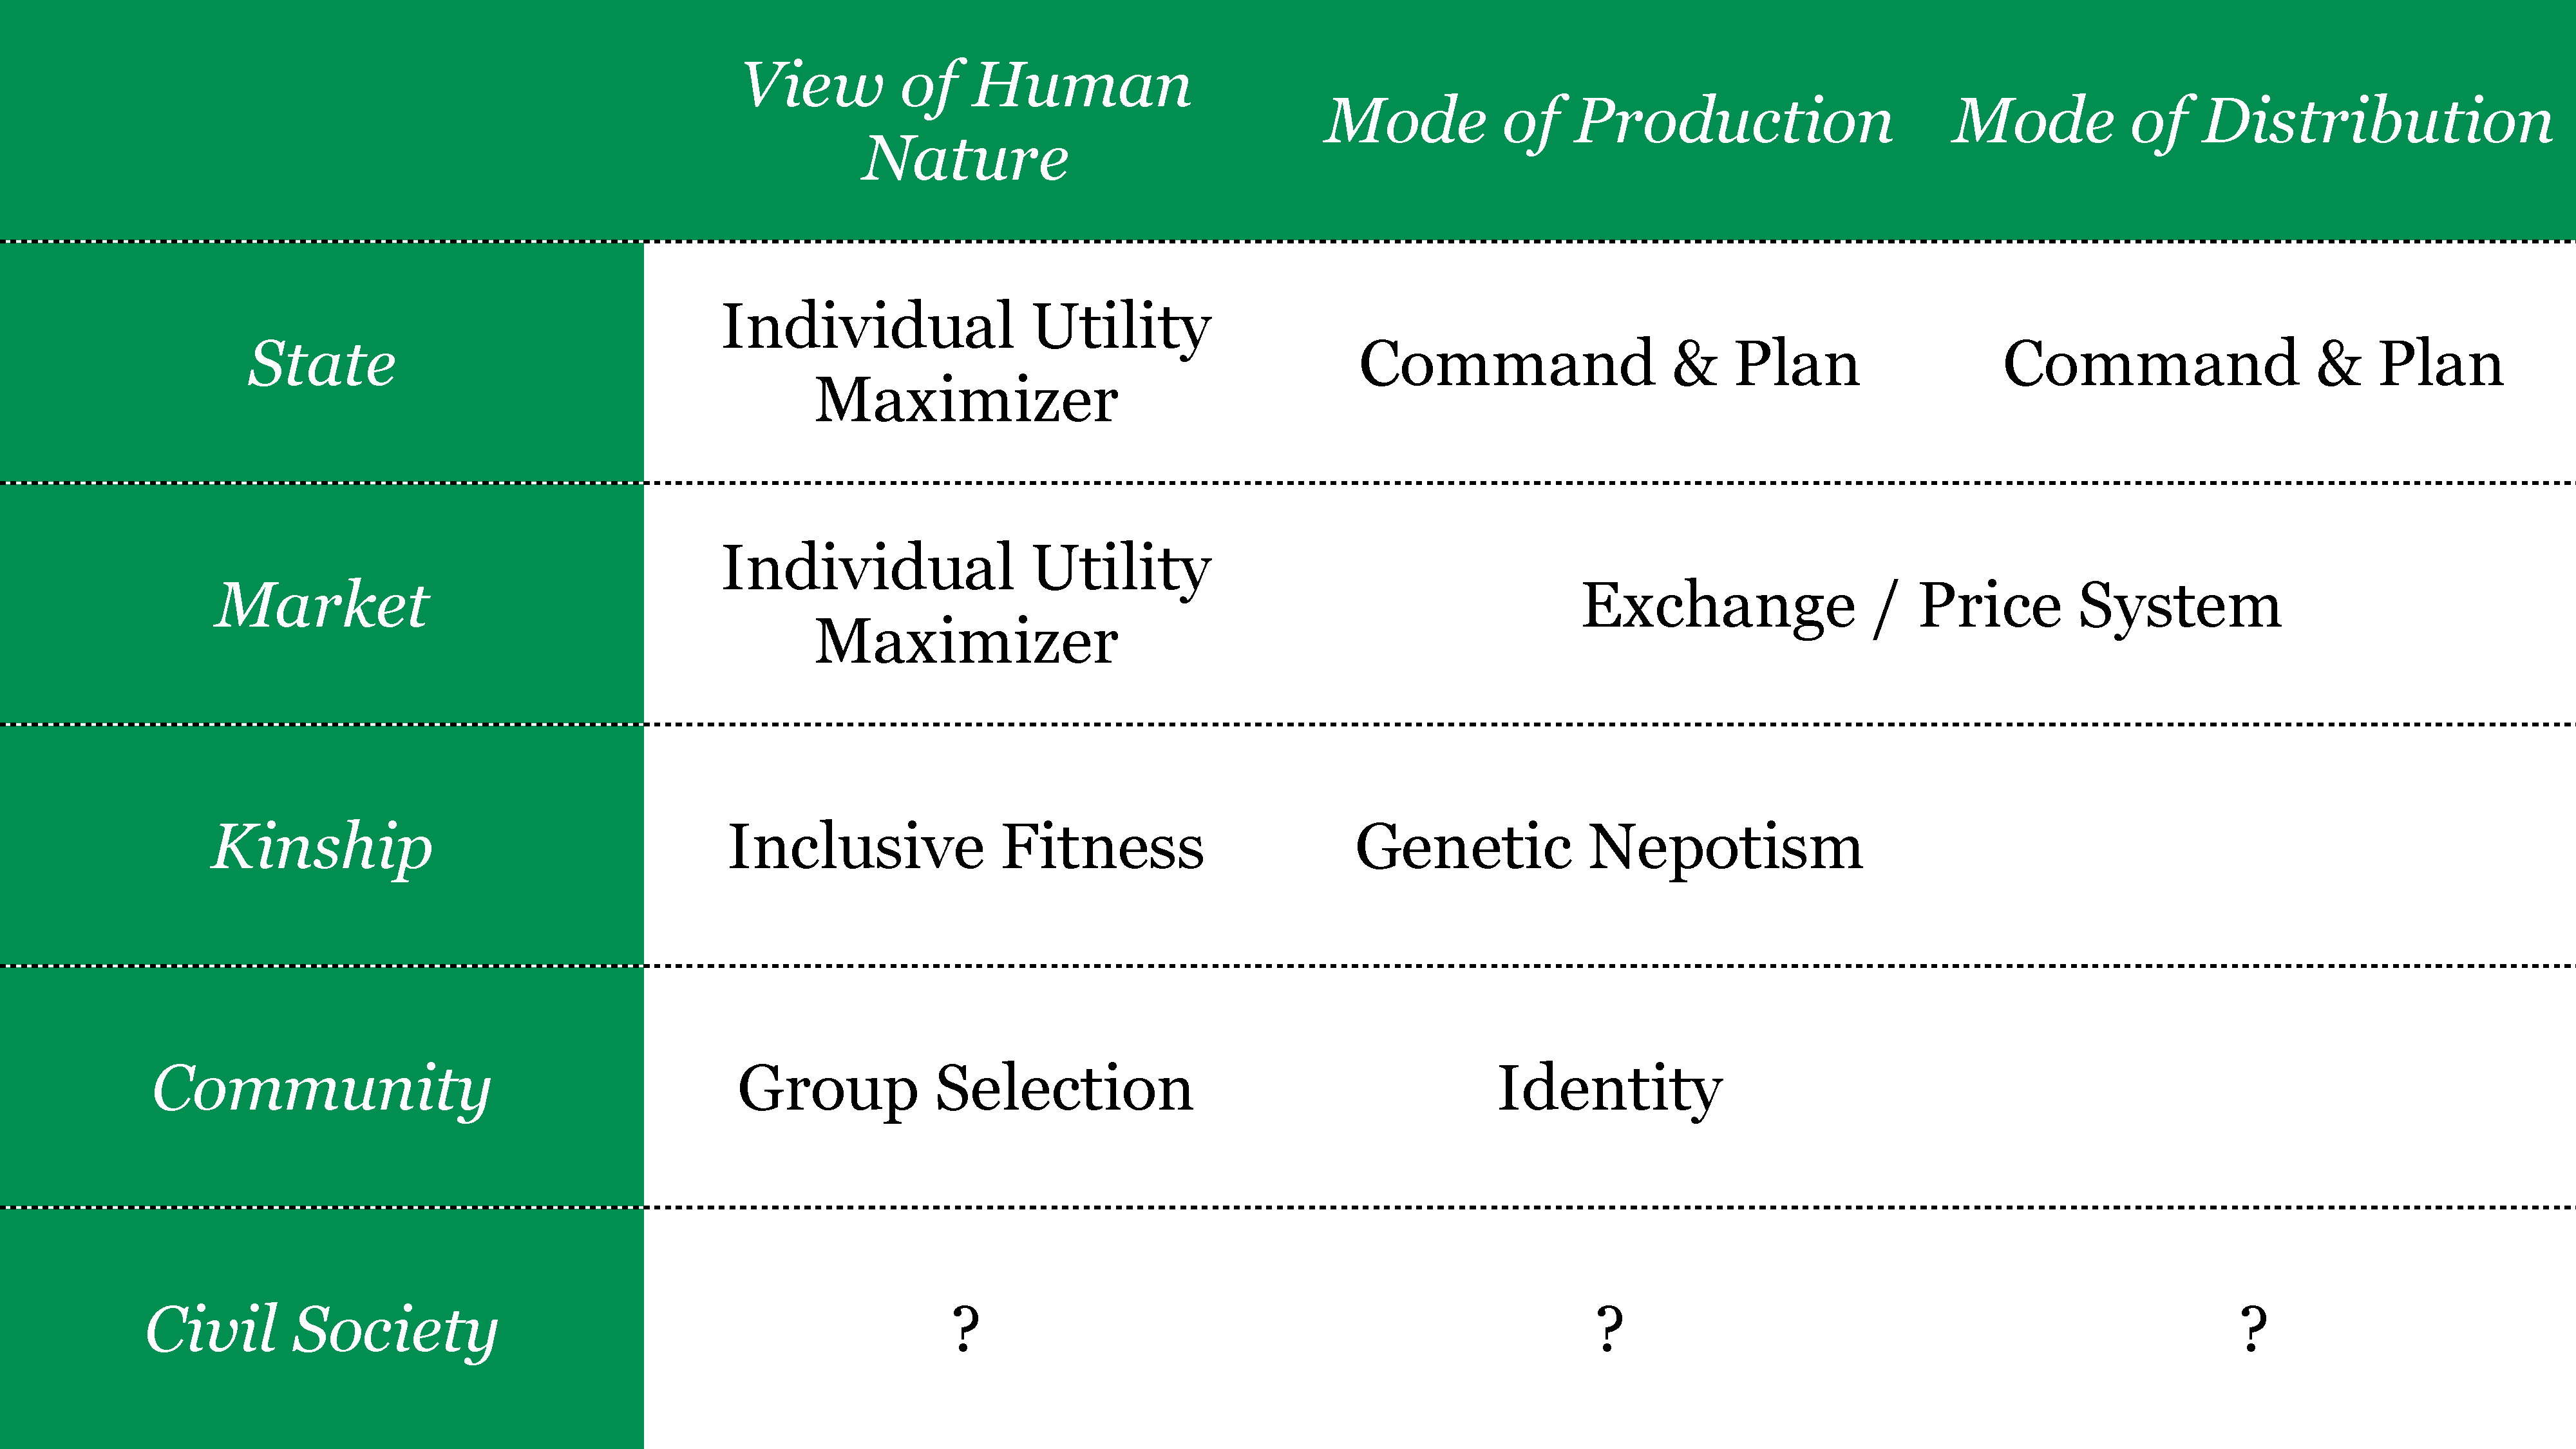
\includegraphics[width=1\linewidth]{modes-human-nature}  
	\caption{Modes of Production, Distribution and Human Nature}
	\label{tab:modes-human-nature}
	\scriptsize{Own summary, but similar to \citeauthor{Schmitter1985} (\citeyear{Schmitter1985}: 52f.).}
\end{table}%remake this table in latex

At the economy or industry level, markets may be our best bet, but perhaps not at the firm or team level, where we can tap into other human motivations. 
Similarly, a state may need to impose health and safety standards, but not a teacher's lesson plan (as \citeauthor{Schwartz2010} alarmingly report). 
Market and state, along with their impoverished view of human nature, \emph{can} be applied selectively, to some domains. 
As alternatives become available
\footnote{
	For example, the \gls{BIG} is a courageous suggestion to, among other things, decommodify \emph{and}, because it is no longer means-tested, ``de-regulate'' the livelihood \citep[for example,][]{Offe2009} and allow volunteerism.
}, 
market and state can recede
\footnote{
	As \citeauthor{Keynes} had promised:
	\begin{quote}
		\emph{``The day is not far off when the economic problem will take the back seat where it belongs, and the arena of the heart and the head will be occupied or reoccupied, by our real problems --- the problems of life and of human relations, of creation and behavior and religion.''}\\*
		--- John Maynard \cite{Keynes}%really, this is undated?
	\end{quote}
}.
For the time being, I suspect, the domains exclusive to market and state will remain considerable. 

In this dissertation, I constrain homo economicus to the realm of the market, and summarize welfare and taxation policies to remedy, as well as make do with its shortcomings. 
In democracy, by contrast, I find a realm in which homo economicus can no longer be accommodated, but where we must instead find new (deliberative) institutions to tap into other, better angels of our nature. %add href

\subsubsection{No New Man} 
Neither policy nor social scientific ontologies can ask for a \emph{new man}. 
For better (see above) or for worse \citep[for example,][]{Schwartz2010}
\footnote{
	\cite{Schwartz2010} show how excessive regulation (the mode of states) and incentives (the mode of markets) can crowd out intrinsic motivation, ``Practical Wisdom'' and other, better angels of our nature. 
	Unfortunately, this ship has probably sailed. 
	Still, their insistence on a broader, human capacity to ``do well by doing good'' and crusade against dehumanizing choice is important.
}
state and market made their own humans: as we live under hierarchy and competition, we adapt to it. 
In the \gls{OECD}-world and in our time, many people (including me) will expect and respond to incentives and regulation. 
Consequently, political institutions have to reckon with homo economicus, even if --- and because --- it is partly of their own making.

Good policy and good social scientific ontology does not ask for a new man, but makes do with the women and men we have now, but at the same time, recognizes that for our ``hypercultural'' species \citep{Henrich2004}, homo economicus, as other views on our indeterminate nature will always be highly \emph{contingent on institutions}. 

None of this is to preclude a study or reform of human nature, modern society, states or markets. 
Rather, such a contingent ontology is, to me, the \emph{only} way to study these meta-institutions and their incarnations in welfare, taxation and democracy. 
\emph{Some}, ontologically contingent homo economicus can clear our hazy eyes, but \emph{too much}, ontologically endogenous homo economicus will blind our ``sociological imagination'' \citep{Mills-1959-aa}. 
Contingency and domain-specificity lead the middle way between the hermetic ideology of utopias, and the apolitical mindlessness of \emph{TINAs}. 

Also, none of this is to proclaim state and market as the ``end of history'' or to blazon homo economicus as ``the last man'' \citep{Fukuyama1992}. 
Rather, state and market along with their homo economicus are the \emph{only} place to start from, if we want to write, or make history in welfare, taxation and democracy today. 
Precisely because our nature is contingent on institutions, that is where we must start: institutions are \emph{all we got}, ``just because institutions are the kinds of things that can can be changed directly, whereas cultures and psychological dispositions are less subject to collective intervention and experimentation'' \citep[K182]{WarrenPearse-2008-aa}. 
States and markets are those prime meta-institutions through which we can make, and remake the institutions of welfare, taxation and democracy. 
Through them, we respond to the homo economicus in all of us, and unfold our greater capacities.

And transcend the limits of homo economicus, we must. 
Clearly, we face grave problems in \hyperref[chap:3-crises]{organizing production and distribution, and in reaching collective decisions} (\autoref{chap:3-crises}, p.~\pageref{chap:3-crises}). 
Clearly, too, disintegration is not an option: that way lies regress and hardship. 
And clearly, further rational-functional or identity-embellished integration is not an option: that way lie democratic deficits, and exclusionary identity politics.

These are the challenges cut out for us. 
To fail them, to fail these cooperation problems of non-zero-sumness, is to fail specifically as a human being, the one ``conspicuously exceptional'' species (\citealt{Frank2011}: 85) that is \emph{socially capable} of great cooperation, but not \emph{biologically determined} to give up individualism \citep{Wright2000}, and is therefore reliant on institutions. 
Welfare, and especially taxation and democracy are those modern institutions, to square the circles of individuality, inequality and cooperation. 

And these are the institutions I here assume to be malleable, to make up the desirable and doable hypotheticals, whose absence begs explanation. 
These, too, are the institutions that moderate the very contingency of homo economicus, and our other natures. 
As such, they are precisely the place to look at, taking on one second-order question at a time, leaving all else to first-order status. 

For sociology, ``the science of institutions, their genesis and their functioning'' \citep[45]{Durkheim1895}, this, I would hope, is a good approach as any to learn --- as we must --- whether, and under which (institutional!) circumstances humans are ``knights, knaves, pawns or queens'' \citep{LeGrand2003}, what our capacity for altruism is \citep{Henrich2007} and how it can be fostered \citep{Axelrod1981a}, all to imagine, and then fulfill our human capacity of non-zero-sumness \citep{Wright2000}.
	\chapter[Mixed Economy]{The Welfare State as Mixed Economy}
		\label{chap:mixed-economy}
		%!TEX root=../tax-democracy-held.tex

\chapter[Mixed Economy]{The Welfare State as Mixed Economy} \label{chap:mixed-economy}

\begin{quote}
	\emph{``The devil may indeed dwell in the details, but we first need to find an angel or two in the abstractions that govern [\ldots]''}
	\\*
	--- Edward J.\ \citet[loc.~117]{McCaffery2002}
\end{quote}

Welfare states are governed by the economic abstractions arising from the co-existence of market and command.

When you organize production and distribution of goods and services by market \emph{and} by command, as welfare states do, the two contradictory systems ``complexly interact'' \citep{Perrow-1999-aa} and easily produce ``unintended consequences'' \citep{Merton-1936-aa} as for example, when \hyperref[sec:price-floors]{minimum wages \emph{may} cause structural unemployment} (p.~\pageref{sec:price-floors}).

To this day, the \emph{mixed economy} of Postwar Western Europe, in its idealized form, is the closest thing to an angel to ever emerge from this uneasy coexistence between market and plan.
To understand first-order desiderata of welfare state design, we need to understand the conceptual compromise of the mixed economy.
Let me first reiterate the logic of its two constituent systems.

\paragraph[Market vs.\ Plan]{Market vs.\ Planned Economy.} \phantomsection \label{sec:market-vs-command}

We can organize economic production and distribution in at least one of two ways,
\begin{inparaenum}
	\item
		by centralized, coercive command or
	\item
		by decentralized, voluntary
		\footnote{
			\label{fn:tilly} This positive description does not imply normatively, as liberal entitlement theory would have it, ``that a person is entitled to those goods acquired in uncoerced exchanges with others'' \citep[149]{Nozick1974,Friedman1962}.
			Uncoerced \emph{exchange} does not mean absence of coersion.
			At the very least, markets rely on a large-scale coercive power (aka. the state) for property rights and states and markets \hyperref[sec:modernity]{\emph{co-evolved} in modernity} \citep{Tilly-1985-aa}.
			Naturalizing whatever allocative results the free market produces as entitled, inalienable, private property is as ahistorical as it is uncritical.
		}
		%href to later desirable discussion, refer back to ontological clarification, also to property debate
		exchange.
\end{inparaenum}

\begin{enumerate}
	\item
		In an ideal-typical \cite{Weber-1920-aa} \emph{command economy}, whoever wields an effective monopoly on the use of force also directs the economy.
		A worker constructs, say, a railroad (production) and is fed by a farmer (distribution), both in fear of --- however indirect --- bodily harm from the monopolist of violence.
		\footnote{
			Because I am  interested in economic abstractions, a materialist theory of the state (such as \citealt{Tilly-1985-aa}) suits me better than, for example, contract theories.
			%reference the edited volume on tax as a source
			Again, this does not imply positive or normative claims.
		}
	\item
		In an ideal-typical \emph{market economy},
		\footnote{
			I prefer the terms ``market'' and ``command'' economy, because the conventional \emph{capital}ism-socialism dichotomy is misleading:
			real existing Soviet (especially Stalinist) socialism also accumulated capital (for example, electrification, railroads), just in different hands.
			Market exchange and planned command describe the different modes of production and distribution more precisely.
		}
		violence is threatened only to maintain property rights and enforce contracts.
			People freely exchange goods and services at equilibrium prices that balance the costs to the producer and the utility to the consumer (\autoref{fig:supply-demand}, p.~\pageref{fig:supply-demand}).
			 A worker constructs a railroad (labor) in return for an enforceable promise to consume (property) a given amount (wage), which he then redeems in a similar exchange with a farmer for food.
\end{enumerate}

\paragraph{Capitalist Welfare State is a Pleonasm.} \phantomsection \label{sec:interface}
Welfare states combine elements of command and market in the service of \emph{equity}.
\footnote{
	Mixed economies also alter market outcomes to improve \emph{efficiency} in case of market failures.
}
Specifically, welfare states coercively adjust the \emph{distributional} outcomes of markets.
\footnote{
	Power resources theory \citep[for example][]{Korpi2003}, Marxist interpretations \citep[for example][]{Offe1972} or recently, some advocates of a \gls{BIG} might disagree:
	for them, the purpose of the welfare state is to change power relations.
	These are reservations of the \hyperref[sec:epistemology]{second-order} (p.~\pageref{sec:epistemology}) and are discussed in \autoref{part:tax-democracy} (p.~\pageref{part:tax-democracy}.
	%are these the right hrefs?
	}
\footnote{
	Conversely, a socialist welfare state is an oxymoron.
	Just as welfare states are defined by their coexistence with a market economy, there is no such thing as a socialist welfare state, no matter the (however corrupted) distributional goals of nominal socialisms.
	In a predominantly planned, or even command economy, the state directs much of both production and distribution and therefore does not require the (welfare state) institutions governing the mixed economy, including taxation, insurance and pension funds, business cycle smoothing and dedicated social service provision.
	Even where these institutions nominally existed, they never faced the (otherwise defining) condition of independent market prices.
	For example, where ``prices'' are \emph{set} and ``profits'' owned by the state, taxes become a meaningless category:
	they are really just changes in the set prices \citep[for example,][23]{Bonker2006}.
}

Welfare states insure their citizens against certain individual risks (disability, sickness, unemployment), fight ``poverty'' by instituting (unconditional or means-tested) minimal living standards and, sometimes, reduce inequality by compressing the income and wealth distribution of the citizenry.

To reach each of these goals, welfare states have to intervene in voluntary exchanges between buyers and sellers.
For better and/or for worse, welfare states change market equilibria.
No matter the legal structure, welfare state institutions never exist \emph{outside} the market:
even ``nationalized''
\footnote{
	A misnomer.
	Even the \gls{NHS} is not fully socialized medicine, it is just a tax-financed near state monopsony on health services.
}
health care needs to buy doctors (at what salary?) and drugs (at what price?) on free markets.
No matter the labeling, welfare state institutions never exist \emph{independently} of the market:
even social ``insurance''.
\footnote{
	In fact, social insurance contributions are a regressive \glsfirst{Payroll}
	%add href, later reference
}
alters labor market outcomes (who should, and can bear the burden?).

Welfare state institutions can interact with markets in more or less attractive ways:
they can have a smaller or larger \glspl{DWL} (\autoref{fig:DWL}, p.~\pageref{fig:DWL}), and they can have well or ill-defined incidences (\autoref{fig:different-incidence}, p.~\pageref{fig:different-incidence}), but they always interact.%improve refs

Welfare state institutions can expand (UK socialized health care) or contract (Germany social health insurance) the scope of its command, but they will always interface with the market at some frontier between the two systems, as illustrated in \autoref{fig:interface-command-market-health} (p.~\pageref{fig:interface-command-market-health}).
This interface is ill-defined, as two incompatible logics collide, twice:

\begin{enumerate}
	\item
		The state demand curve (dashed in green) for doctors or hospitals breaks down, as the marginal utility of an additional doctors to citizens (the ultimate consumers) cannot be known.
		\footnote{
			Individual citizens are incentivized to mis(over)-represent their marginal utility from additional doctors, absent individually accruing costs.
			This is equivalent to a \gls{CPR} problem or the cooperation problem of a \gls{PD}.
		}
		The state therefore has to determine the citizenry demand, usually based on a \gls{CBA} or a related procedure --- all of which are really nothing but fancy names for sophisticated economic planning.
	\item
		The state cannot \emph{command} the required supply (of doctors or hospitals), but must instead \emph{buy} the supply from state revenues on free markets.
		\footnote{
			\ldots or socialize parts of the labor market, which would further shift the frontier, but not alleviate the problem.
		}
		Again, the logic of the market breaks down:
the state as the only buyer (of doctors or hospitals) creates a monopsony, causing distributive effects (to the disadvantage of doctors or hospitals) and welfare losses (a \gls{DWL}).
		Alternatively --- maybe more plausibly --- the producers of medical care may capture the planning body and extract rents, distributing away from the public and also causing a welfare loss.
		Either way, pricing poses unavoidable problems:
somewhere down the line, producers require a price, but without atomistic demand, no pareto-optimizing price can be found.
		This is not to say that if health care --- or some other welfare service --- \emph{were} completely privatized, such pareto-optimal equilibrium \emph{would} be reached.
		In fact, government procurement of health and other services can be understood as a response to \hyperref[failed atomistic markets]{sec:market-failures} \emph{for} these goods (p.~\pageref{sec:market-failures}).
		Arguably, government procurement replaces one (horrendous) market failure with another, (milder) form of failure.
\end{enumerate}

\begin{landscape}
 \begin{figure}[htbp]
	\begin{center}
	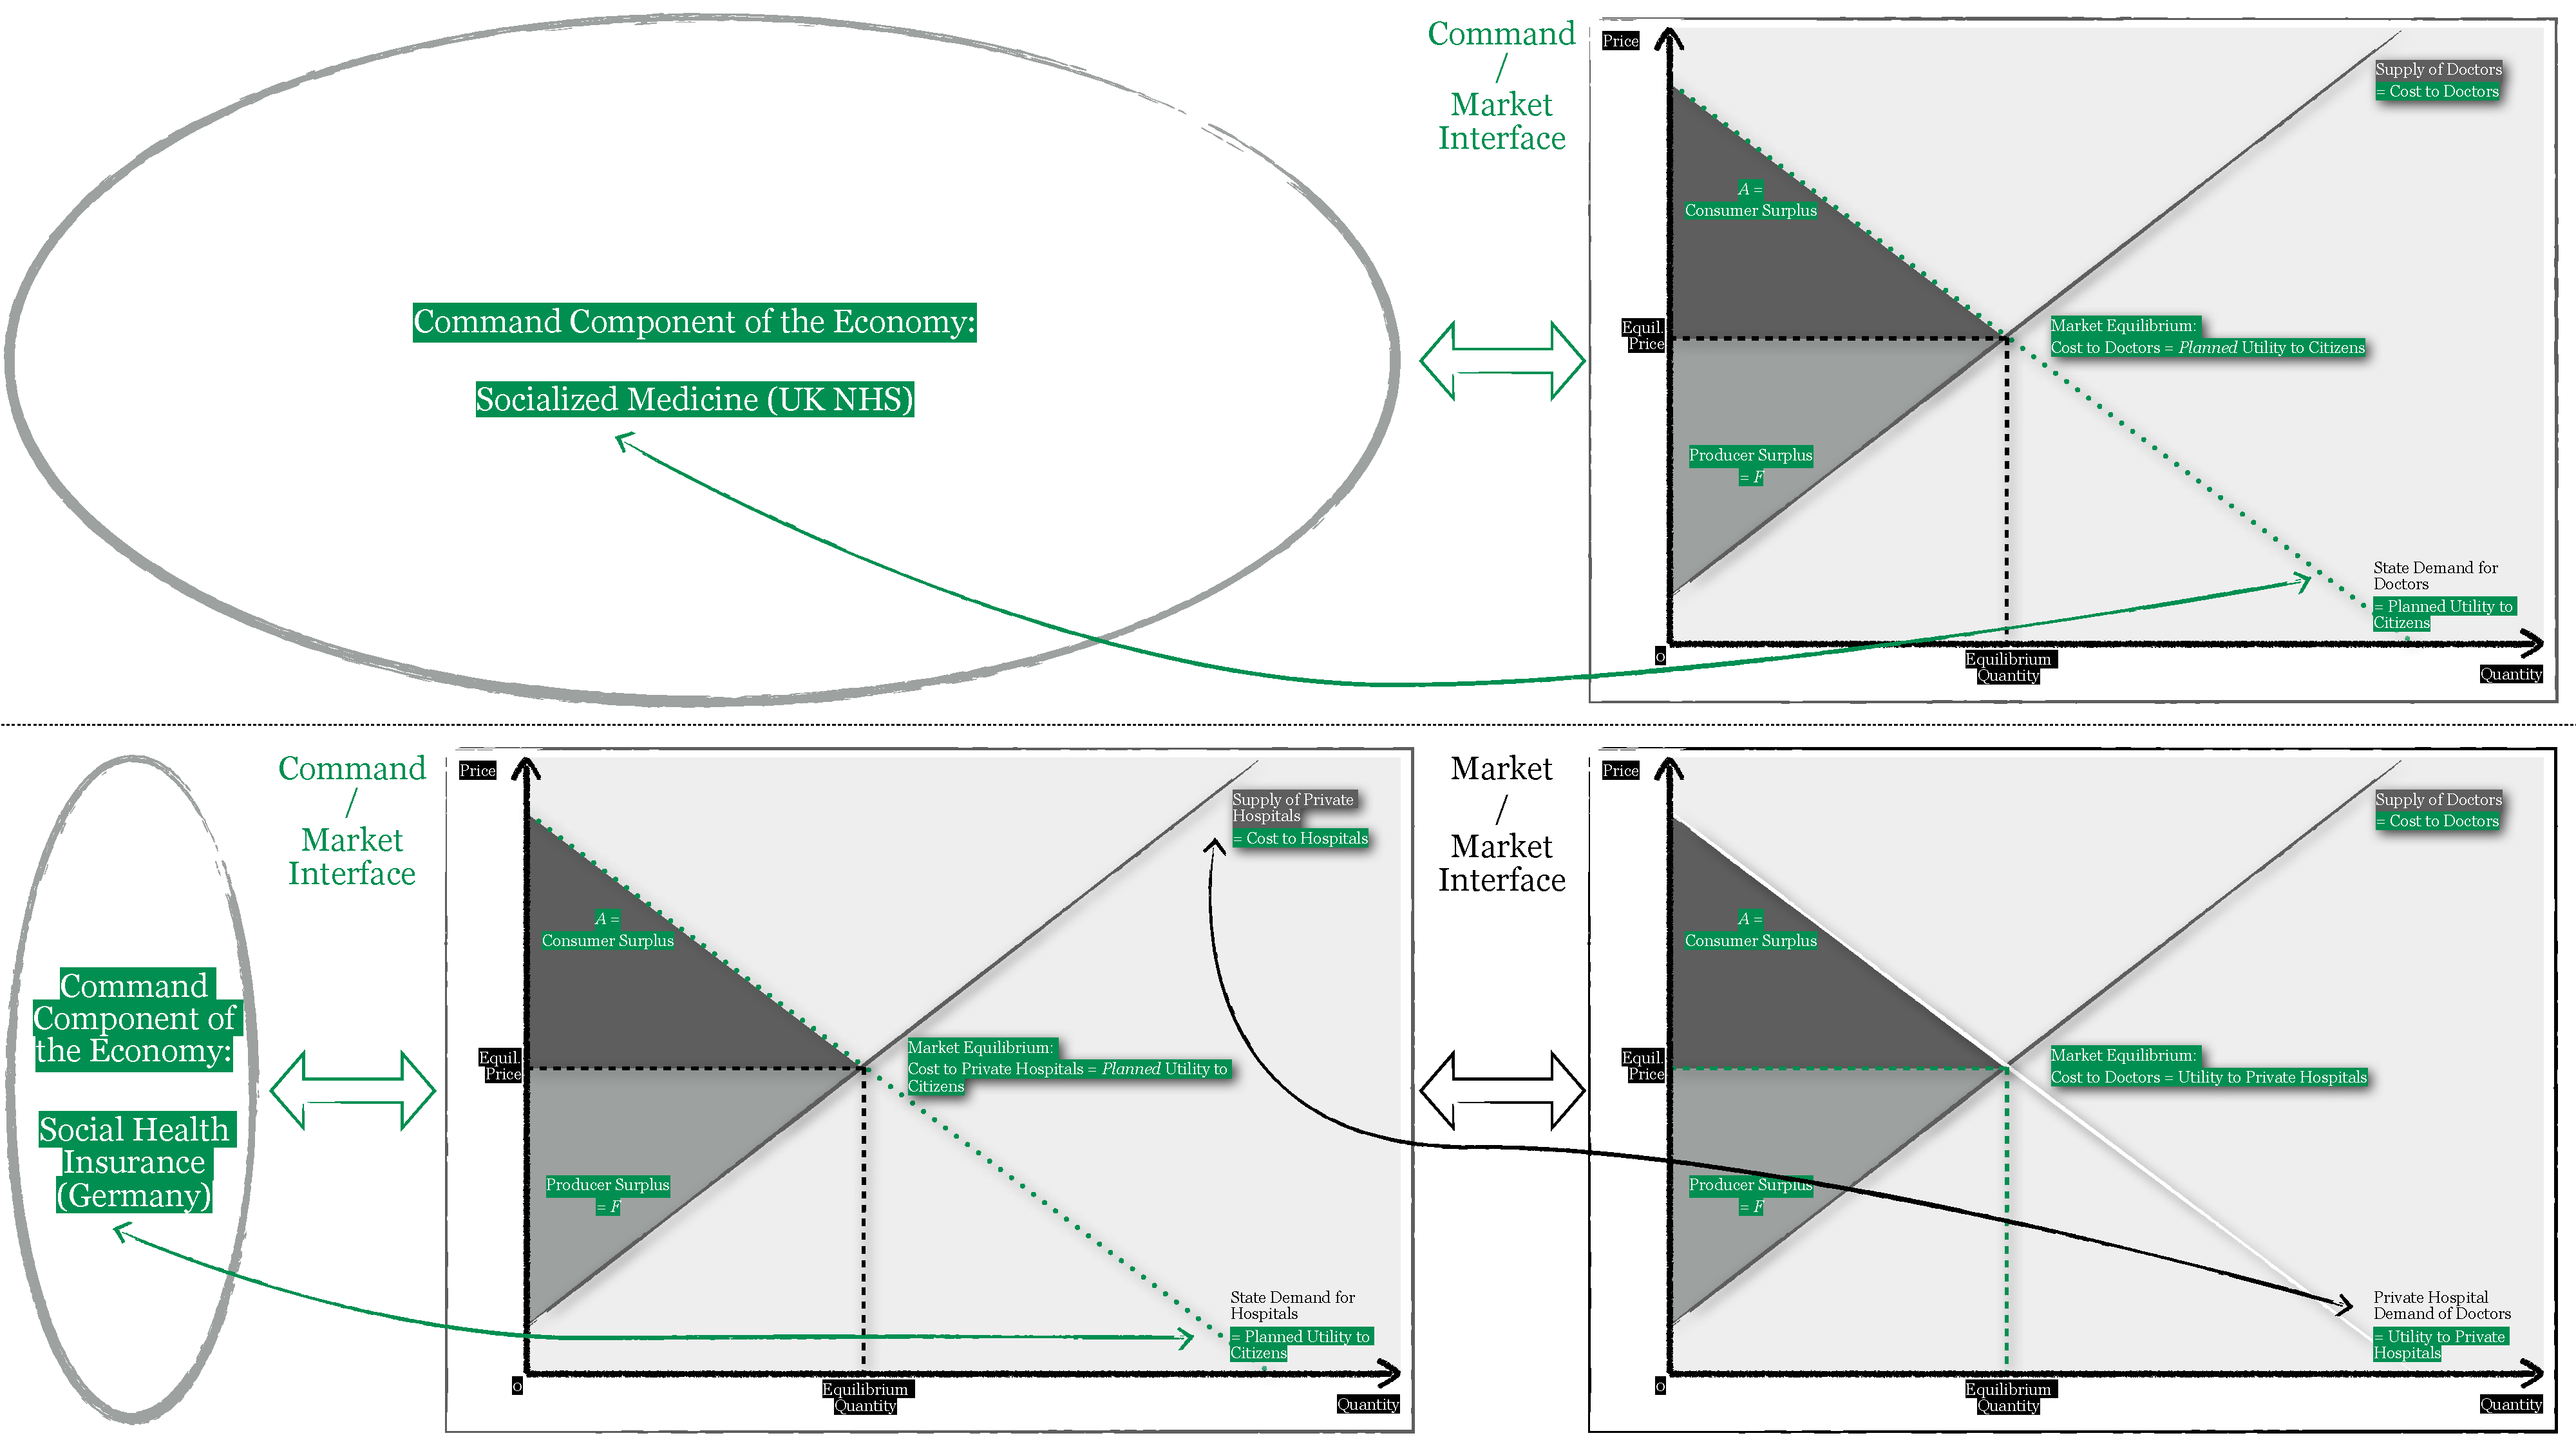
\includegraphics[width=1\textheight]{interface-command-market-health}
	\caption[Command-Market Interface in UK and German Healthcare]{The Command-Market Interface in UK and German Healthcare}
	\label{fig:interface-command-market-health}
	\end{center}
\scriptsize{
	Market supply and demand are drawn in a conventional price-quantity diagram.
	For a larger version, see \autoref{fig:supply-demand} (p.~\pageref{fig:supply-demand}).
	I discuss the \hyperref[sec:market-solutions-production]{competitive market equilibrium} later (p.~\pageref{sec:market-solutions-production}).}
\end{figure}
\end{landscape}

I aim here to distill for welfare, what Edward \citeauthor{McCaffery2002} urges us to do about tax:
``to find an angel or two in the abstractions that govern [\ldots]'' \citeyearpar[K117]{McCaffery2002}.

I look for these angels in an \emph{ideal} closed, mixed economy.
The account I provide in the \hyperref[chap:mixed-economy]{following pages} (p.~\pageref{chap:mixed-economy}) -- \pageref{sec:EU-reality}) does not resemble any \emph{real} existing economy, where abstractions are often shrouded in historical idiosyncrasies, and angels rarely found amidst imperfect policies.
But this is a question of the \hyperref[sec:1st-questions-first]{first order} (p.~\pageref{sec:1st-questions-first}), and to know what is materially doable and normatively desirable we need \hyperref[itm:a-priori]{a priori reason} (p.~\pageref{itm:a-priori}), not a posteriori reality.

Even without the details, the abstractions alone need considerable space to be explained.
I urge readers to take the time, even if much will seem familiar and some things appear remote to welfare, let alone taxation or democracy.
They are not:
from \hyperref[sec:adverse-selection]{adverse selection} (p.~\pageref{sec:adverse-selection}) to \hyperref[sec:winner-take-all]{winner-take-all} network effects (p.~\pageref{sec:winner-take-all}), \hyperref[sec:why-mixed-economy-matters]{it all matters} (p.~\pageref{sec:why-mixed-economy-matters}).
Missing any one of these abstractions, we cannot know what welfare and taxation can, and should do.

\paragraph{Disclaimer}
Four disclaimers apply to my tentative answer on this very big question:\phantomsection \label{sec:disclaimers}

\begin{enumerate}
	\item \label{itm:not-original} \emph{Not Original}.
		The perspective I take here is hardly original.
		Many others have, in greater width \citep{Stiglitz2002} or depth \citep{Sinn2004}, with narrower \citep{Scharpf1997} or different foci \citep{Zurn-2000-aa} discussed the first-order shortcomings of ``negative'' integration (in the \gls{EU}:
\citealt{Scharpf1997}), and economic liberalization everywhere \citep{Stiglitz2002}, and have, in that context, defined the conditions of a mixed economy.

	I aim here to review the works of others and to restate some fairly conventional economic concepts in order to build a first-order checklist of welfare state design.

	\item \label{itm:no-test} \emph{No Positive Test}.
		I cannot myself muster the methodological rigor or provide the econometric data, to test the first-order theories of welfare state design, but rely on mainstream literature instead.

		The economics of the welfare state are vastly complex, incompletely understood and any policy initiative requires careful (empirical) investigation to balance the often contradictory imperatives of economic policy.

		Moreover, as I later find for taxation, reforms of the magnitude implied herein may strain against the current limits of economic science:
experimental designs lack in external validity of a vastly complex modern economy and simulations often lack the data, or even computing power to model such inframarginal changes.
%reference that section

	\item \label{itm:no-calibration} \emph{No Calibration}.
		I offer no calibration of the mixed economy and its institutions, and, for the purpose of this chapter, advocate no \emph{particular} balance between market and state, efficiency and equity or any of the other trade-offs a mixed economy may face.
		Instead, I highlight the capacities and dysfunctions of markets and \hyperref[sec:ends]{list the state institutions} \emph{potentially} able to mitigate these shortcomings (p.~\pageref{sec:ends}).
		I consider under \hyperref[sec:means]{which conditions these institutions can work} (p.~ \pageref{sec:means}) and hypothesize how they might explain the \hyperref[chap:3-crises]{threefold crises of welfare, democracy and taxation} (\autoref{chap:3-crises}, p.~\pageref{chap:3-crises}).

	\item \label{itm:little-macroeconomics} \emph{Little Macroeconomics.}
		I limit this discussion to very basic concepts of the real economy, and ignore many of the more complex models, especially of finance and money.
		Modern macroeconomics, including such powerful frameworks as the IS/LM model are important \citep[originally][]{Hicks1937}, but would go beyond the already lengthy treatment here.
		%explain

		I also suspect and hope that macroeconomics is best investigated by experts and its policy imperatives safely implemented by technocrats.
		Monetary policy, for instance, may not raise deep normative questions or offer vexing trade-offs in need of democratic adjudication:
its imperatives hinge on contested and imperfect, but merely first-order, positive findings on a mass psychology of price and cost signals (see \autoref{itm:empirical-macroeconomics}, p.~\pageref{itm:empirical-macroeconomics}).
		To a lesser extent, finance, too, may be politically epiphenomenal:
money and other property rights move in tandem \emph{with}, and are \emph{secondary} to material economic exchanges in the ideal mixed economy (see p.~\pageref{itm:epiphenomenal-finance}).
		To the extent that polities can agree on specific and measurable objectives (such as price stability, or risk diversification), macroeconomic policy really can be delegated to independent central banks or other regulatory bodies.

		By limiting the discussion to a few rudimentary, but deeply understood concepts of the real economy, I also hope to reconnect regional integration and the welfare state to an \emph{econonomic imagination} \citep[paraphrasing][]{Mills-1959-aa} of our material affairs as a household --- only with a cast of billions.
		\footnote{
			\ldots as the etymology of economics would suggest:
the science of managing the \emph{oikos}, greek for household.
		}

		Inevitably, much of the detail and complexity that policy makers have to consider, will fall by the wayside.
\end{enumerate}
%needs ueberleitung

\section[Ends]{The Ends of a Mixed Economy} \label{sec:ends}

\footnote{\label{fn:also-in-mpp}
	This section is based, in part, on earlier, unpublished work which I submitted to the Hertie School of Governance as my Master of Public Policy thesis in \citep{Held2010a}.
	I have since revised and expanded it.
}

\begin{quote}
	\emph{``Adam Smith needs revision, Gentlemen."}
	\\*
	%find better quote?
	--- Fictional John Nash (*1928) in \emph{A Beautiful Mind} (2001)
\end{quote}

If the defining characteristic of a welfare state is its uneasy union of market and plan, we must first understand the broader interplay of exchange and command in the mixed economy.
\autoref{tab:ends-mixed-economy} (p.~\pageref{tab:ends-mixed-economy}) summarizes exchange (or market) and command (or state) institutions to address five material dimensions of the human condition:
\hyperref[sec:production]{production} (p.~\pageref{sec:production}), \hyperref[sec:risk]{risk} (p.~\pageref{sec:risk}), \hyperref[sec:distribution]{distribution} (p.~\pageref{sec:distribution}), \hyperref[sec:time]{time} (p.~\pageref{sec:time}) and \hyperref[sec:space]{space} (p.~\pageref{sec:space}).
This is a slightly expanded set, inspired by \citeauthor{MusgThet1959}'s \citeyearpar{MusgThet1959} seminal definition of basic public policy functions:
allocation/efficiency, distribution and stabilization (for example, as cited in \citep[4]{Bordo2011}.
It also corresponds to \citeauthor{Samuelson-1954-eu}'s authoritative textbook \citeyearpar[recently][]{Samuelson2005} desiderata of a mixed economy:
\begin{enumerate}
	\item to let scarce resources be efficiently allocated by \emph{competitive markets},
	\item to improve the equity of market outcomes through \emph{redistribution},
	\item to provide \emph{public goods} by government procurement and
	\item to limit inherent market instability by financial regulation and well-directed monetary and fiscal policies
\end{enumerate} \citep[as cited in][K532]{Stiglitz2011}.

%!TEX root=../tax-democracy-held.tex

\begin{landscape}
 \begin{table}[htbp]
	\begin{center}
	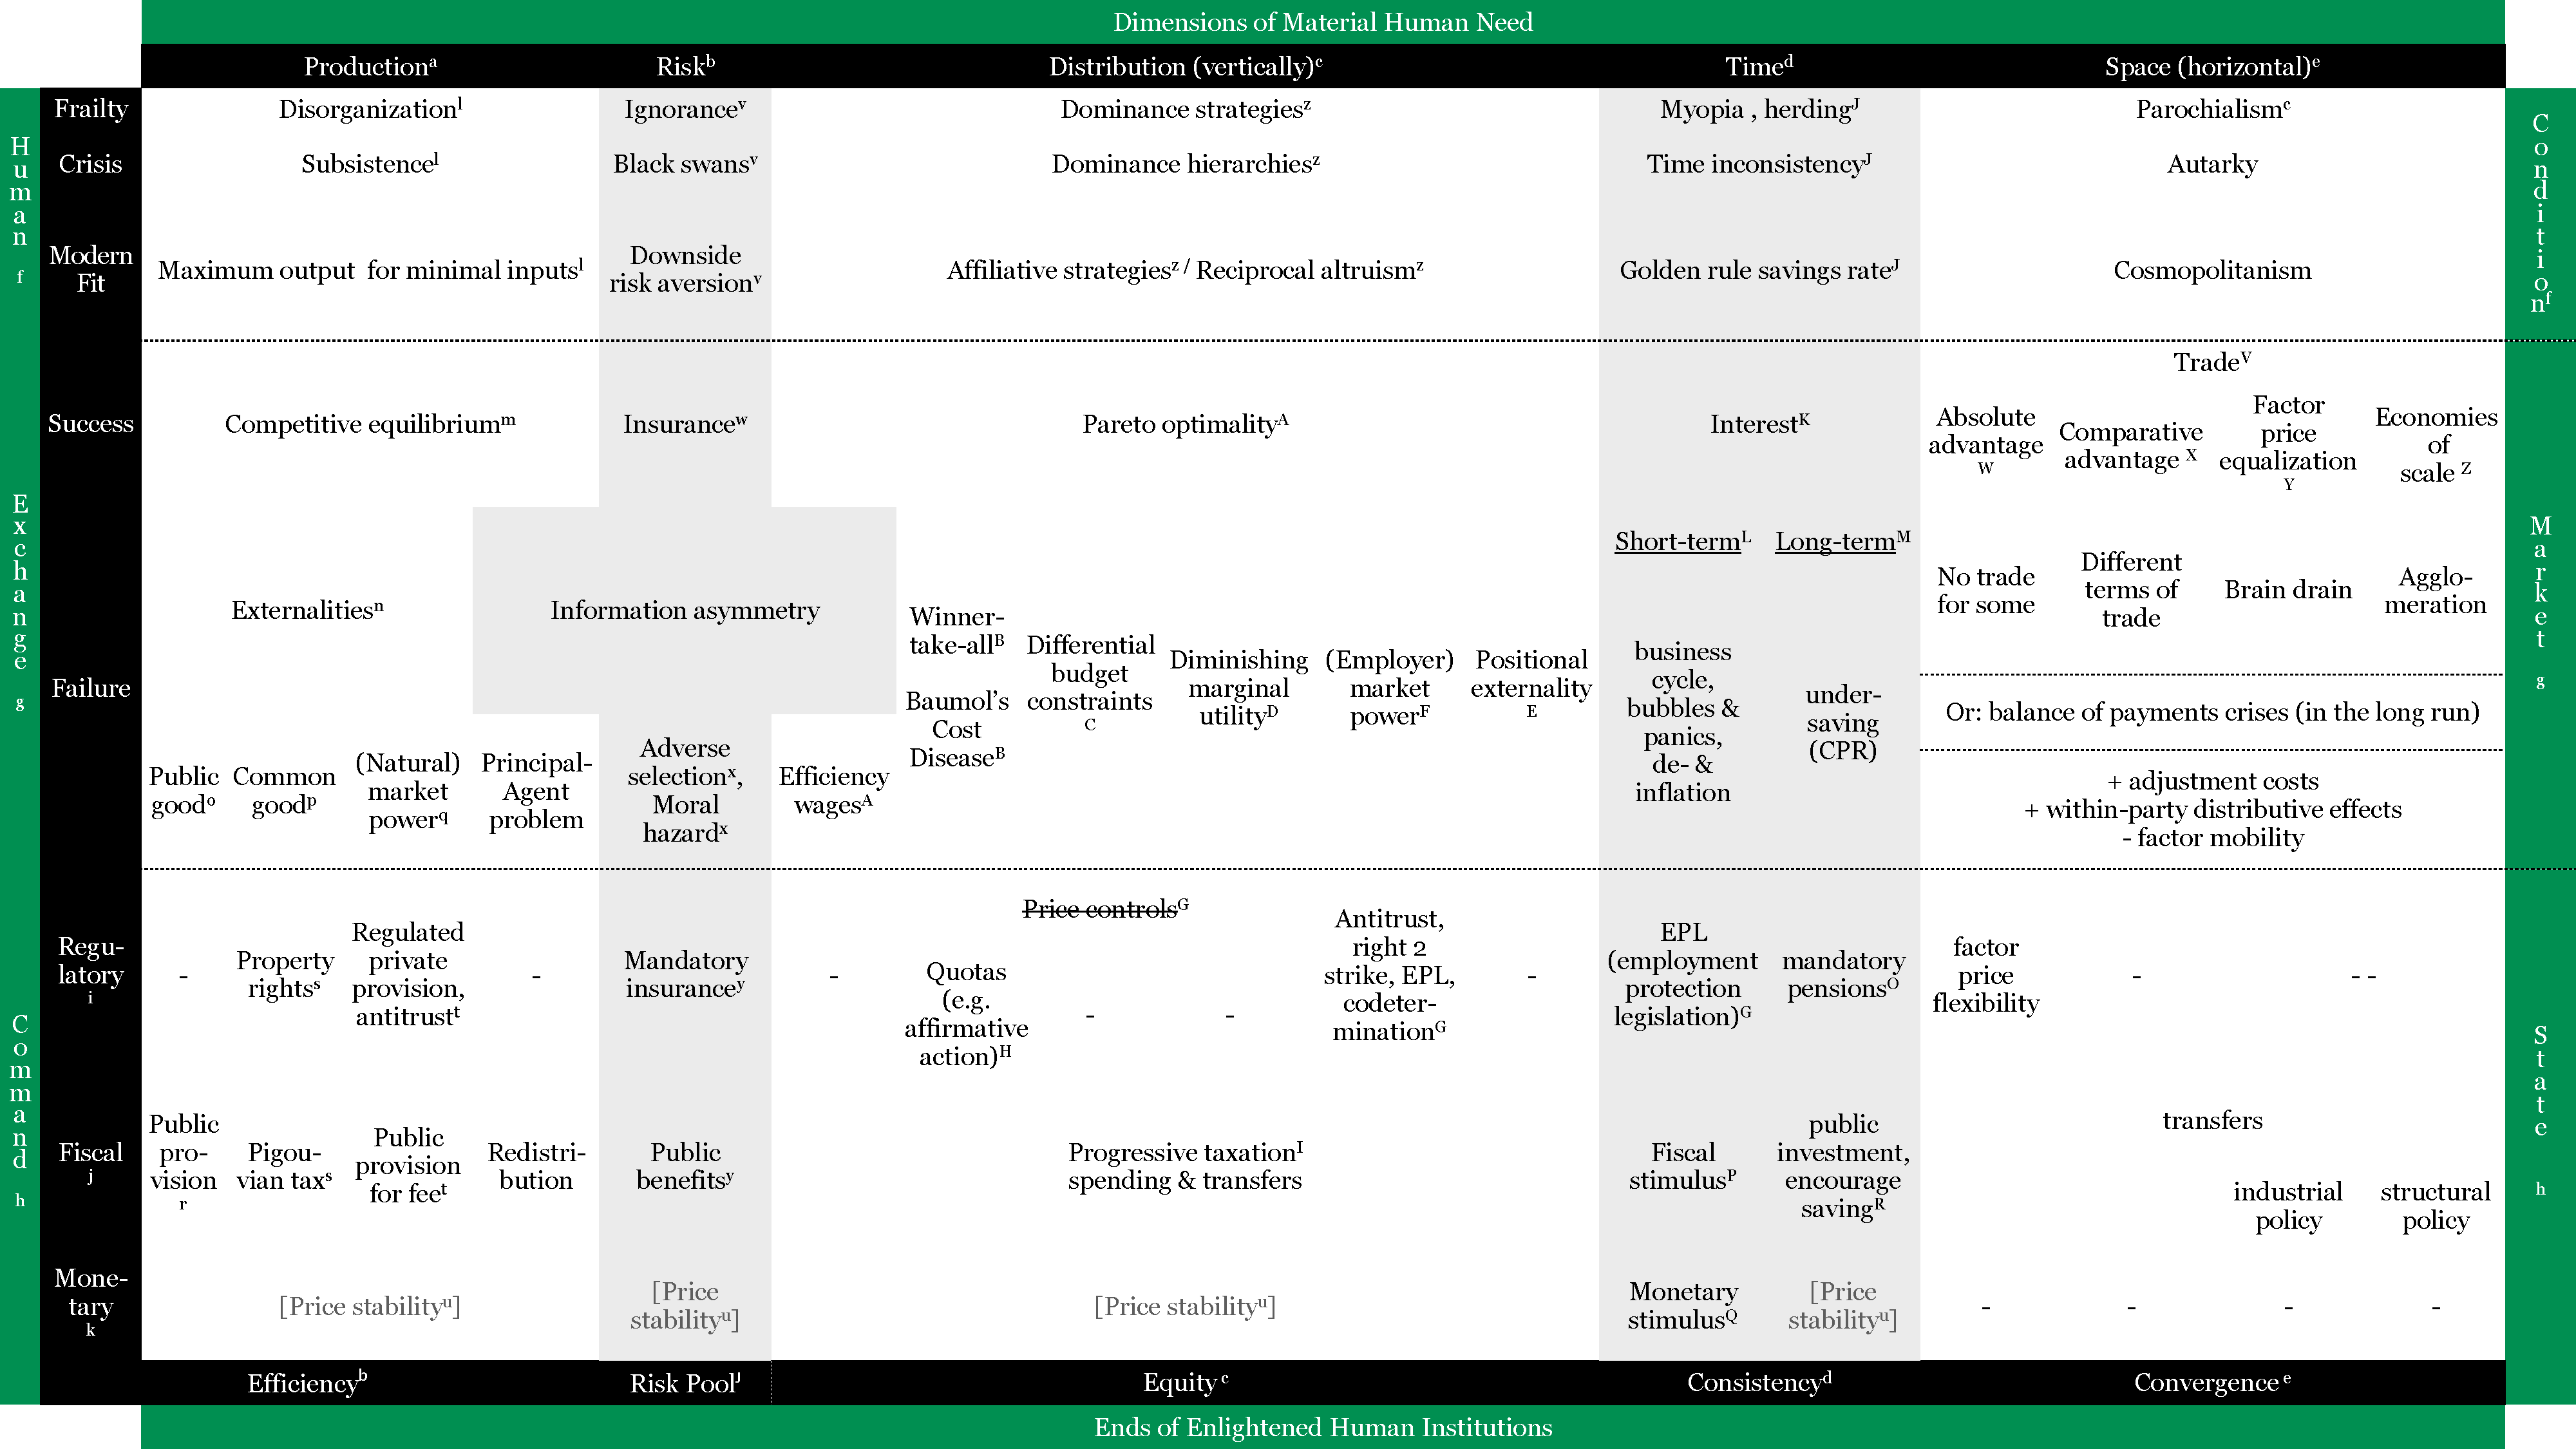
\includegraphics[width=1\linewidth]{ends-mixed-economy}
	\caption{Ends of the Mixed Economy \label{tab:ends-mixed-economy}}
\end{center}
\newpage
\end{table}
\end{landscape}\footnote{
Read the table from top to bottom, then from left to right. For every material dimension (column), I first present the human condition (first three rows), then market (exchange) solutions and problems (next two rows) and then present corresponding state (command) responses by fiscal, regulatory and monetary means (bottom three rows). The headings of following sections correspond to the column headings.

		\emph{a}: \nameref{sec:production} on page \pageref{sec:production},
		\emph{b}: \nameref{sec:risk} on page \pageref{sec:risk},
		\emph{c}: \nameref{sec:distribution} on page \pageref{sec:distribution},
		\emph{d}: \nameref{sec:time} on page \pageref{sec:time},
		\emph{e}: \nameref{sec:space} on page \pageref{sec:space},
		\emph{f}: \nameref{sec:human-condition} on page \pageref{sec:human-condition},
		\emph{g}: \nameref{sec:exchange} on page \pageref{sec:exchange},
		\emph{h}: \nameref{sec:command} on page \pageref{sec:command},
		\emph{i}: \nameref{sec:regulatory} on page \pageref{sec:regulatory},
		\emph{j}: \nameref{sec:fiscal} on page \pageref{sec:fiscal},
		\emph{k}: \nameref{sec:monetary} on page \pageref{sec:monetary},
		\emph{l}: \nameref{sec:human-nature-of-production} on page \pageref{sec:human-nature-of-production},
		\emph{m}: \nameref{sec:market-solutions-production} on page \pageref{sec:market-solutions-production},
		\emph{n}: \nameref{sec:market-failures} on page \pageref{sec:market-failures} and see \autoref{tab:types-of-goods},
		\emph{o}: \nameref{sec:public-good} on page \pageref{sec:public-good},
		\emph{p}: \nameref{sec:common-good} on page \pageref{sec:common-good},
		\emph{q}: \nameref{sec:natural-monopoly} on page \pageref{sec:natural-monopoly},
		\emph{r}: \nameref{sec:public-good-response} on page \pageref{sec:public-good-response},
		\emph{s}: \nameref{sec:common-good-response} on page \pageref{sec:common-good-response},
		\emph{t}: \nameref{sec:natural-monopoly-response} on page \pageref{sec:natural-monopoly-response},
		\emph{u}: \nameref{sec:price-stability} on page \pageref{sec:price-stability},
		\emph{v}: \nameref{sec:human-nature-of-risk} on page \pageref{sec:human-nature-of-risk},
		\emph{w}: \nameref{sec:insurance} on page \pageref{sec:insurance},
		\emph{x}: \nameref{sec:asymmetric-information} on page \pageref{sec:asymmetric-information},
		\emph{y}: \nameref{sec:state-insurance} on page \pageref{sec:state-insurance},
		\emph{z}: \nameref{sec:human-nature-of-inequality} on page \pageref{sec:human-nature-of-inequality},
		\emph{A}: \nameref{sec:market-equity} on page \pageref{sec:market-equity},
		\emph{AA}: \nameref{sec:efficiency-wages} on page \pageref{sec:efficiency-wages},
		\emph{B}: \nameref{sec:winner-take-all} on page \pageref{sec:winner-take-all},
		\emph{C}: \nameref{sec:different-budget-constraints} on page \pageref{sec:different-budget-constraints},
		\emph{D}: \nameref{sec:diminishing-marginal-utility} on page \pageref{sec:diminishing-marginal-utility},
		\emph{F}: \nameref{sec:monopsony-employers} on page \pageref{sec:monopsony-employers},
		\emph{E}: \nameref{sec:positional-race} on page \pageref{sec:positional-race},
		\emph{G}: \nameref{sec:price-controls} on page \pageref{sec:price-controls},
		\emph{H}: \nameref{sec:affirmative-action} on page \pageref{sec:affirmative-action},
		\emph{I}: \nameref{sec:fiscal-redistribution} on page \pageref{sec:fiscal-redistribution},
		\emph{J}: \nameref{sec:time} on page \pageref{sec:time},
		\emph{K}: \nameref{sec:interest} on page \pageref{sec:interest},
		\emph{L}: \nameref{sec:short-term-inconsistency} on page \pageref{sec:short-term-inconsistency},
		\emph{M}: \nameref{sec:long-term-inconsistency} on page \pageref{sec:long-term-inconsistency},
		\emph{O}: \nameref{sec:government-saves} on page \pageref{sec:government-saves},
		\emph{P}: \nameref{sec:fiscal-stimulus} on page \pageref{sec:fiscal-stimulus},
		\emph{Q}: \nameref{sec:monetary-stimulus} on page \pageref{sec:monetary-stimulus},
		\emph{R}: \nameref{sec:government-saves} on page \pageref{sec:government-saves},
		\emph{S}: \nameref{sec:government-saves} on page \pageref{sec:government-saves},
		\emph{V}: \nameref{sec:trade} on page \pageref{sec:trade},
		\emph{W}: \nameref{itm:absolute-advantage} on page \pageref{itm:absolute-advantage},
		\emph{X}: \nameref{itm:comparative-advantage} on page \pageref{itm:comparative-advantage},
		\emph{Y}: \nameref{itm:FPE} on page \pageref{itm:FPE},
		\emph{Z}: \nameref{itm:NTT} on page \pageref{itm:NTT}.}

% \begin{table}[htbp]
	%	\centering
	%	\rotatebox{90}{
	%	\begin{minipage}{\textheight}
	%	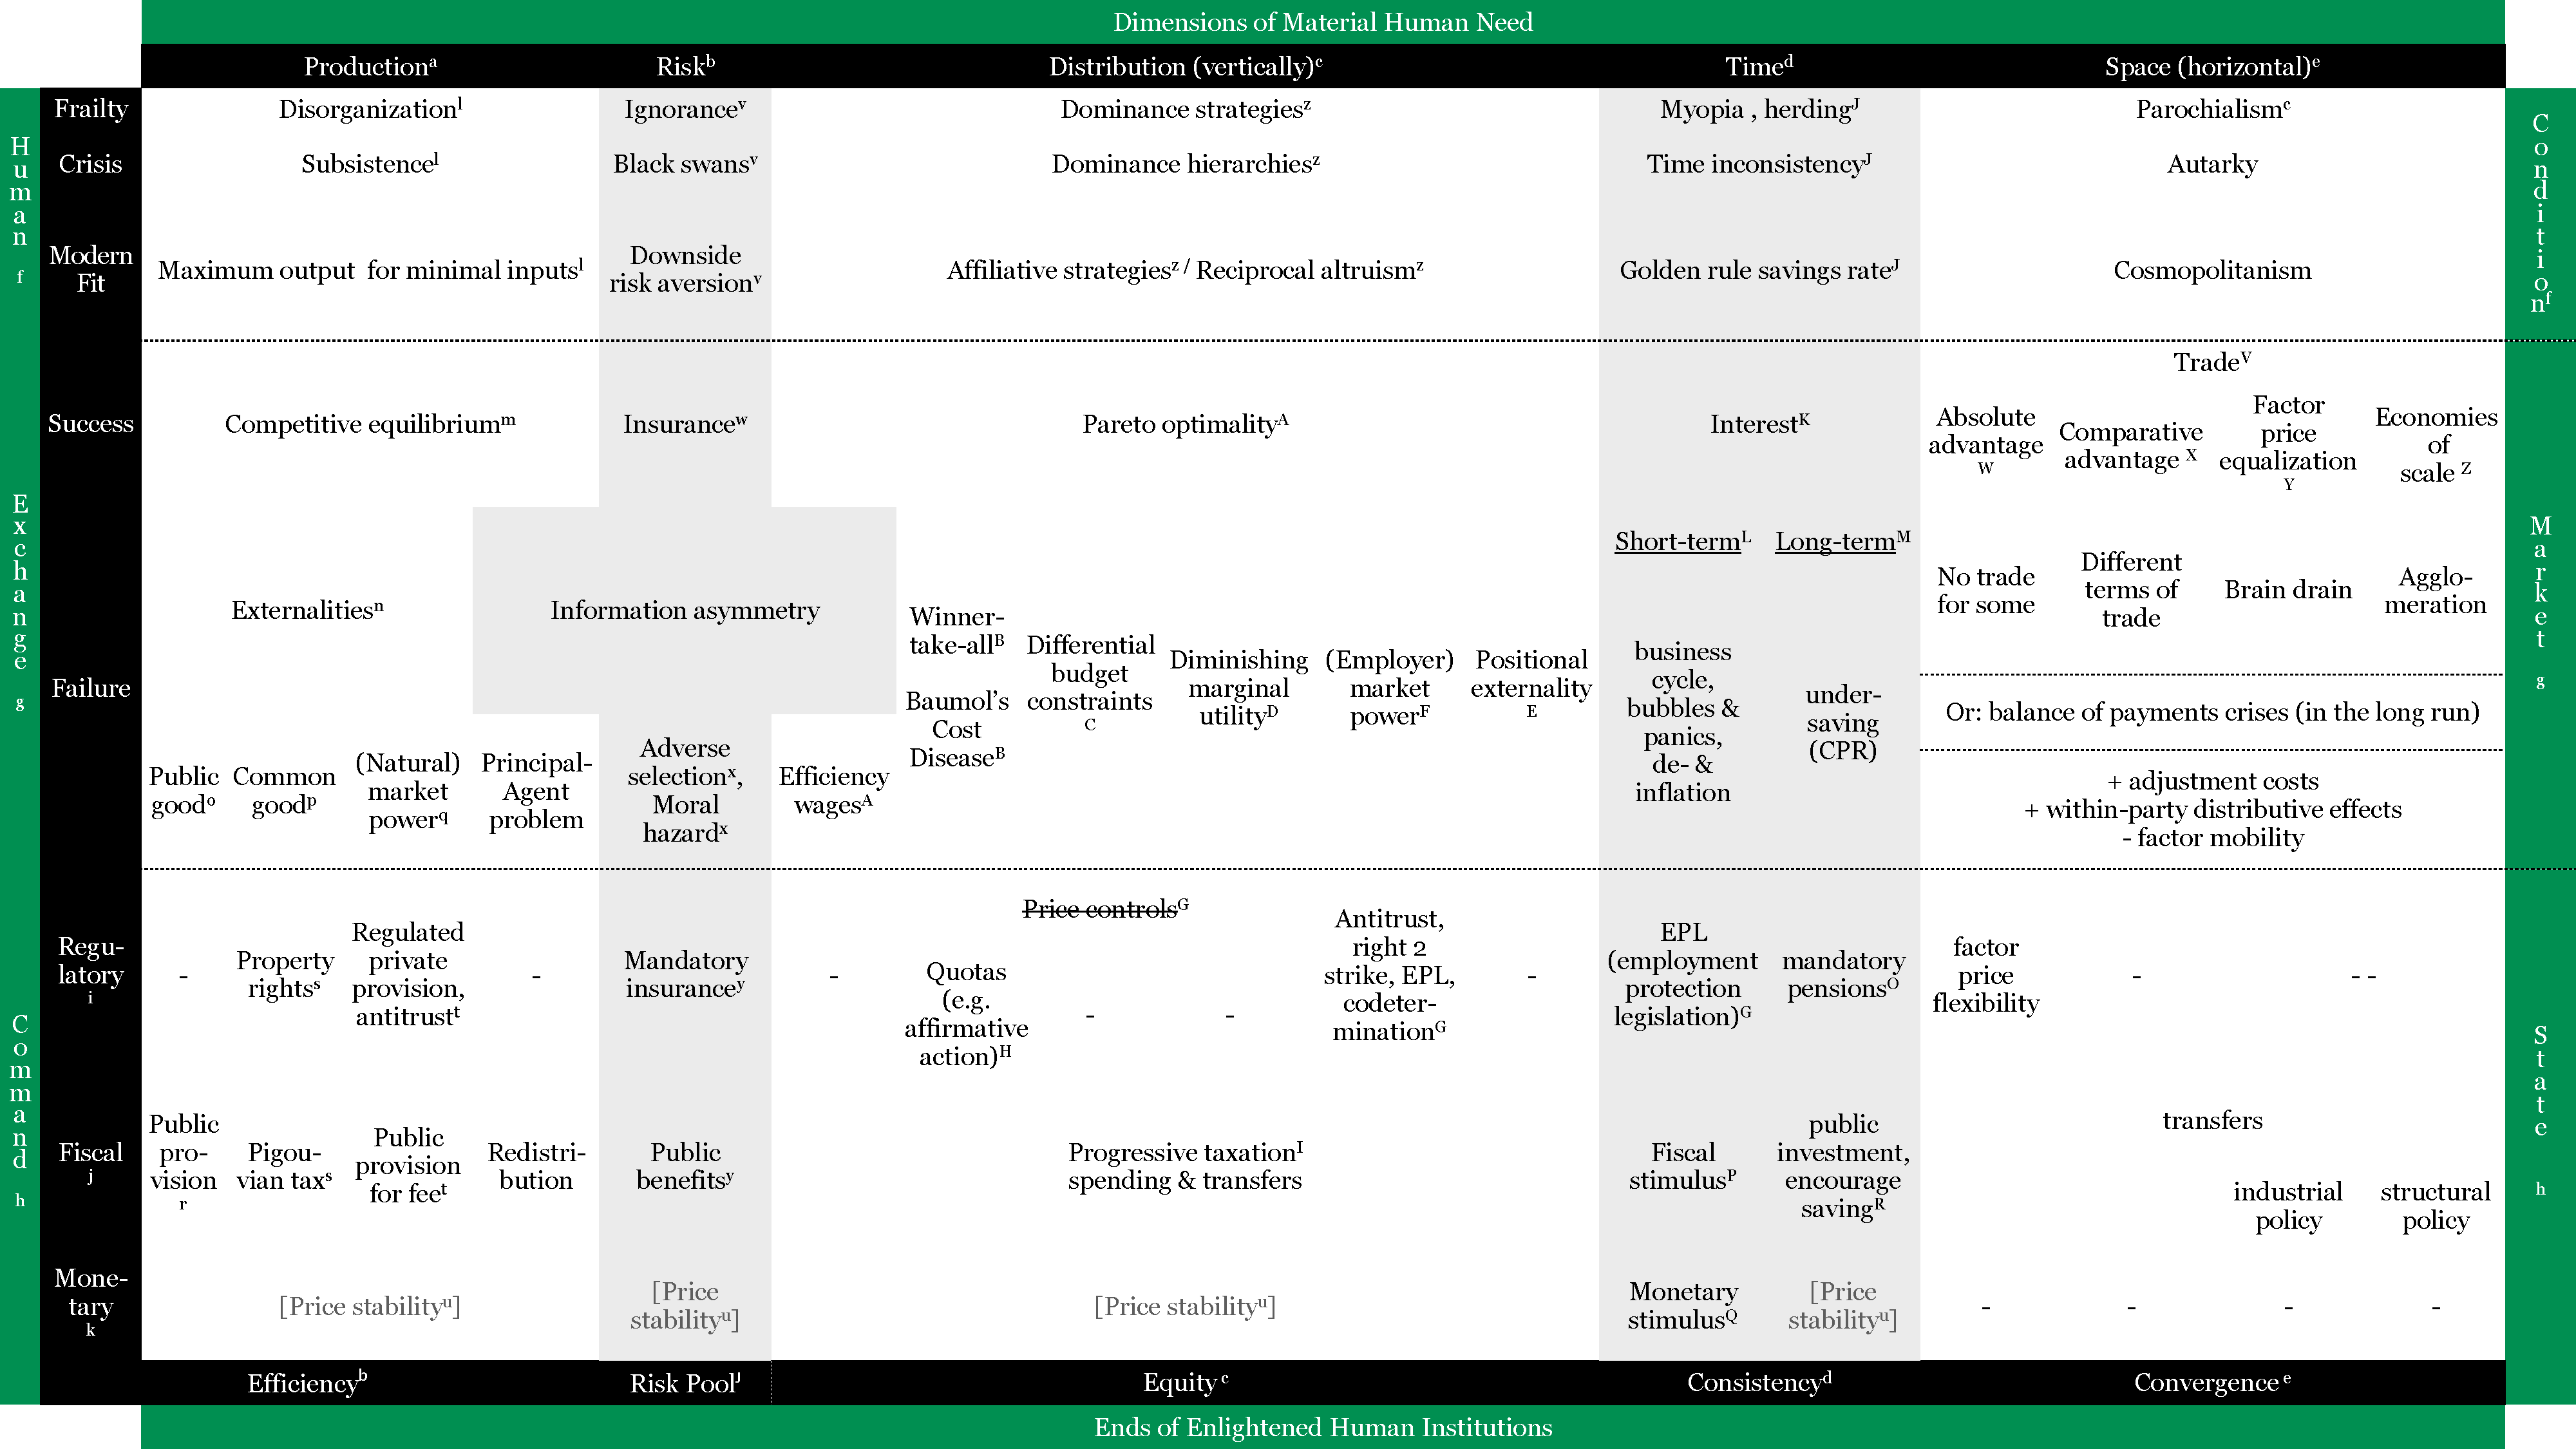
\includegraphics[width=1\linewidth]{ends-mixed-economy}
	%	\caption{Ends of the Mixed Economy}
	%	\label{tab:ends-mixed-economy}
	%	\end{minipage}
	%	}
%\end{table}

%\includepdf[landscape=true , fitpaper=true, frame=true ]{ends-mixed-econ}
	%if you want to go back and use this, you have to enable pdfpages package

%this needs to be improved, great cuts required b/c much may already be in ontology.
\paragraph{The Human Condition.} %already defined:
%\label{sec:human-nature}
Humans are a frail and feeble species and depend on a favorable physical and social environment (fit) to thrive.
Exactly what the frailties of the human condition
\footnote{\label{fn:human-condition}
	I choose the term ``human condition'', because it captures what might be (positively) inescapable in human existence, without specifying either a natural or cultural explanation.
}
are is of course controversial.
I ground the mixed economy in human needs (rows 1--3 in \autoref{tab:ends-mixed-economy}) to provide context.
\footnote{
	Some of the frailties follow the heuristics and biases of human cognition identified by the prospect theory research program \citep{KahnemanTversky1979,Kahneman2011
}

	Prospect theory is appropriate to consider for any first-order theory on the material:
it provides a positively descriptive model of human cognition and decision making as opposed to the normatively optimal (but rarely observed) expected utility hypothesis, on which neoclassical economics rest (first formulated by \citealt{Bernoulli1738}, later specified by \citealt{VonNeumannMorgenstern1944}).

	In part, the mixed economy and the welfare state (for example, mandatory pensions) are institutions to get prospect theory humans, easily mislead by their fast but erroneous ``system one'' to follow the slow, but accurate ``system two'' \citep{Kahneman2011}).
	Supposedly, when we give it some thought, we find that decisions based on expected utility \citep{Bernoulli1738} maximize our happiness, but ever the ``cognitive misers'' \citep{FiskeTaylor-1991-aa}, exhausted and overwhelmed, we easily fall back to \emph{system one} shortcuts and fail to rationally maximize utility.
	Institutions, characteristically enabling and restricting human behavior --- including those of the mixed economy --- can help prospect theory humans to approximate decisions based on expected utility.

	Prospect theory, alas, is still an emerging field (together with yet dejunct evolutionary psychology and cognitive neuroscience), and any link to the mixed economy must in the meantime remain tenuous.
}
and to focus on the first-order ends (bottom row) that the institutions of the mixed economy are to serve on these five dimensions (columns):
\emph{efficient} \hyperref[sec:production]{production}, \emph{precaution} against \hyperref[sec:risk]{risk}, an \emph{equitable} \hyperref[sec:distribution]{distribution}, \emph{consistency} over \hyperref[sec:time]{time} and \emph{convergence} over \hyperref[sec:space]{space}.
%add pagerefs

\paragraph[Exchange]{Exchange.} \phantomsection \label{sec:exchange}
Markets organize production by institutionalized, voluntary exchange of private property rights.
They orchestrate both the production and the distribution of goods in \emph{one} system (rows 4--6).
Markets \hyperref[sec:market-solutions-production]{succeed} when they efficiently allocate resources and, equivalently, effectively process dispersed information.
Markets also \hyperref[sec:market-failures]{fail}, cause excessive inequity and risky imbalances.

\paragraph[Command]{Command.} \phantomsection \label{sec:command}
The mixed economy is the set of \hyperref[sec:regulatory]{regulatory} (p.~\pageref{sec:regulatory}), \hyperref[sec:fiscal]{fiscal} (p.~\pageref{sec:fiscal}) and \hyperref[sec:monetary]{monetary} (p.~\pageref{sec:monetary}) policies to mitigate market failures and to alter undesirable distributive outcomes (rows 6--8).

\paragraph{State-Market Coevolution.} \autoref{tab:ends-mixed-economy} does not imply a historical or conceptual primacy of the market over the state, or vice versa.
%also redundant b/c ontoloty
Production and distribution by exchange did not necessarily predate production and distribution by command, they \hyperref[sec:modernity]{\emph{co-evolved}} (\citealt{Tilly-1985-aa}, also \autoref{sec:modernity}).
Likewise, production and distribution by command is no more a stop-gap measure to failures of a market economy than market provision is a stop-gap to government waste.
\footnote{
	Indeed, as Dr.~Mildner of the Hertie School of Governance never tired of telling me:
	``There is state failure, too''
	%ask for permission to quote
}

\autoref{tab:ends-mixed-economy} and this entire \autoref{chap:mixed-economy} could be reorganized to start out with command solutions and problems, to which market institutions then respond.
For example, governments may be inapt at producing diverse and fashionable clothing,
\footnote{
	As suggested by the late \href{http://kimjongillookingatthings.tumblr.com/}{Kim-Jong Il's choice of grey jumpsuits}.
}
which is then spun off to markets.
Neither markets nor states are generally superior, they are just better modes of producing and distributing \emph{different} things.

As \autoref{tab:ends-mixed-economy} stands, the game appears stacked against the market, as there is no list of government failures.
In fact, failures abound in the command economy:
without credible information about individual utility \citep[confer][]{Hayek1931}, and an elegant mechanism for their aggregation  \citep[confer][]{Lerner1944, Lange1934, Debreu1954} resources are easily wasted and misallocated and even command components in market economies are prone to \emph{government failure} \citep{Coase1964}.
Moreover, a market economy seems to be closely related to liberal democracy,
\footnote{
	As in modernization theory, for example, \cite{InglehartWelzel-2005-aa}.
}
and bloated command economies may corrupt politics,
\footnote{
	Specifically, resource-based ``rentier states'' may hinder liberal democracy \citep{Beblawi1990}.
	Generally, distributive decisions in planned economies appear easily as zero-sum games (as opposed to the per-definition non-zero-sum, pareto improvements in competitive markets), which may corrupt politics.
	%add href
}
or even threaten the very constitution of freedom \citep{Hayek1944, Friedman1962}.

Here again --- to ``economize on moral disagreement'' \citep[K226]{GutmannThompson-2004-aa} and to lend credence to my later conclusions --- I conservatively place the burden of proof on the state:
production and distribution by markets should \emph{only} be replaced or altered by command when the market can demonstrably not achieve the desired outcomes, that is, when problems materialize (row 4 in \autoref{tab:ends-mixed-economy}).

I now discuss the five material dimensions of human need in turn.

\subsection[Efficient Production]{Efficient Production:\ Growing the Pie}\label{sec:production}

\paragraph{The Human Condition of Production}\phantomsection \label{sec:human-nature-of-production}
Cooperative production offers great non-zero-sum gains for humans, but does not come to us robotically, as much else \citep{Wilson2012}.
And so, again, we need institutions to regulate our cooperation.
%this is also discussed earlier already, ref this
Without them, we are left in a debilitating state of \emph{disorganization} (column 1, row 1 in \autoref{tab:ends-mixed-economy}).

Under \hyperref[itm:pragmatic-ethics]{ethical pragmatism} (p.~\pageref{itm:pragmatic-ethics}) and \hyperref[sec:utilitarianism]{preliminary utilitarianism} (p.~\pageref{itm:utilitarianism}), humans must strive for institutions that deliver \emph{maximum outputs for minimal inputs}
\footnote{
	This broad definition of efficiency is more demanding than pareto efficiency.
	%other efficiency and equity norms are further discussed in \ldots add \href
}
(see column 1, row 3 in \autoref{tab:ends-mixed-economy}, p.~\pageref{tab:ends-mixed-economy}).
%pageref

\paragraph{Market Solutions to Production.} \phantomsection \label{sec:market-solutions-production}
Assuming, as I do, \hyperref[sec:contingent-homo-economicus]{contingent homo economicus} (p.~\pageref{sec:contingent-homo-economicus}) and conditions for \hyperref[sec:perfect-competition]{perfect competition} (p.~\pageref{sec:perfect-competition}) markets have at least two attractive properties:
\footnote{
	Here, as always, it is important to keep up \hyperref[sec:epistemology]{epistemological hygiene} (p.~\pageref{sec:epistemology}).
	The first theorem of welfare economics invoked here is an exercise in positive logic.
	It does not imply:
	\begin{enumerate}
		\item
			that \emph{actual} markets display these properties --- that would be a first order \emph{empirical}, not logical finding.
			The assumptions of \hyperref[sec:perfect-competition]{perfect competition} are, in fact, quite heroic and may rarely be observed in the real world.
		\item
			that market allocations are beyond normative reproach.
			The first theorem of welfare economics, crucially, operates only on \emph{ex ante} distributions, which may or may not be distributively just.
	\end{enumerate}
}
\begin{enumerate}
	\item
		when all  participants have made all profitable exchanges,
		\footnote{
			(Neo)classical economics takes an oddly static view of the economy.
			In reality, equilibria are more often in flux, a matter of becoming, not being.
		}
		markets produce at the quantity and price where the costs to the producers equal the willingness to pay of buyers (see \autoref{fig:supply-demand}, p.~\pageref{fig:supply-demand}).
		Consumers and producers in any given market enjoy maximum \emph{surplusses}:
all consumers pay prices (at least incrementally) below the utility they receive (by area $A$), all producers receive prices (at least incrementally) above the costs they incur (by area $F$).
		In this \emph{competitive equilibrium} (see column 1, row 4 in \autoref{tab:ends-mixed-economy}, p.~\pageref{tab:ends-mixed-economy}), no one can be made better off without making someone else worse off:
it is \emph{Pareto optimal}.
		\footnote{\label{fn:1st-theorem}
			Formally, the first theorem of welfare economics states that over a \emph{given} distribution, the competitive equilibrium will be a pareto optimum (demonstrated first graphically by \cite{Lerner1944}, mathematically by \cite{Lange1934}, \cite{Debreu1954} and others).
		}
		\footnote{
			An allocation is pareto-improved if at least someone receives more, with others receiving (at least) the same.
			When all such improvements are exhausted, an allocation is pareto optimal.
			Crucially, pareto improvements and optimality are always in reference \emph{only} to some ex-ante allocation.
			Also, pareto improvements do not imply that everyone would be better off by the same amount.
		}
	\begin{figure}[htbp]
		\centering
		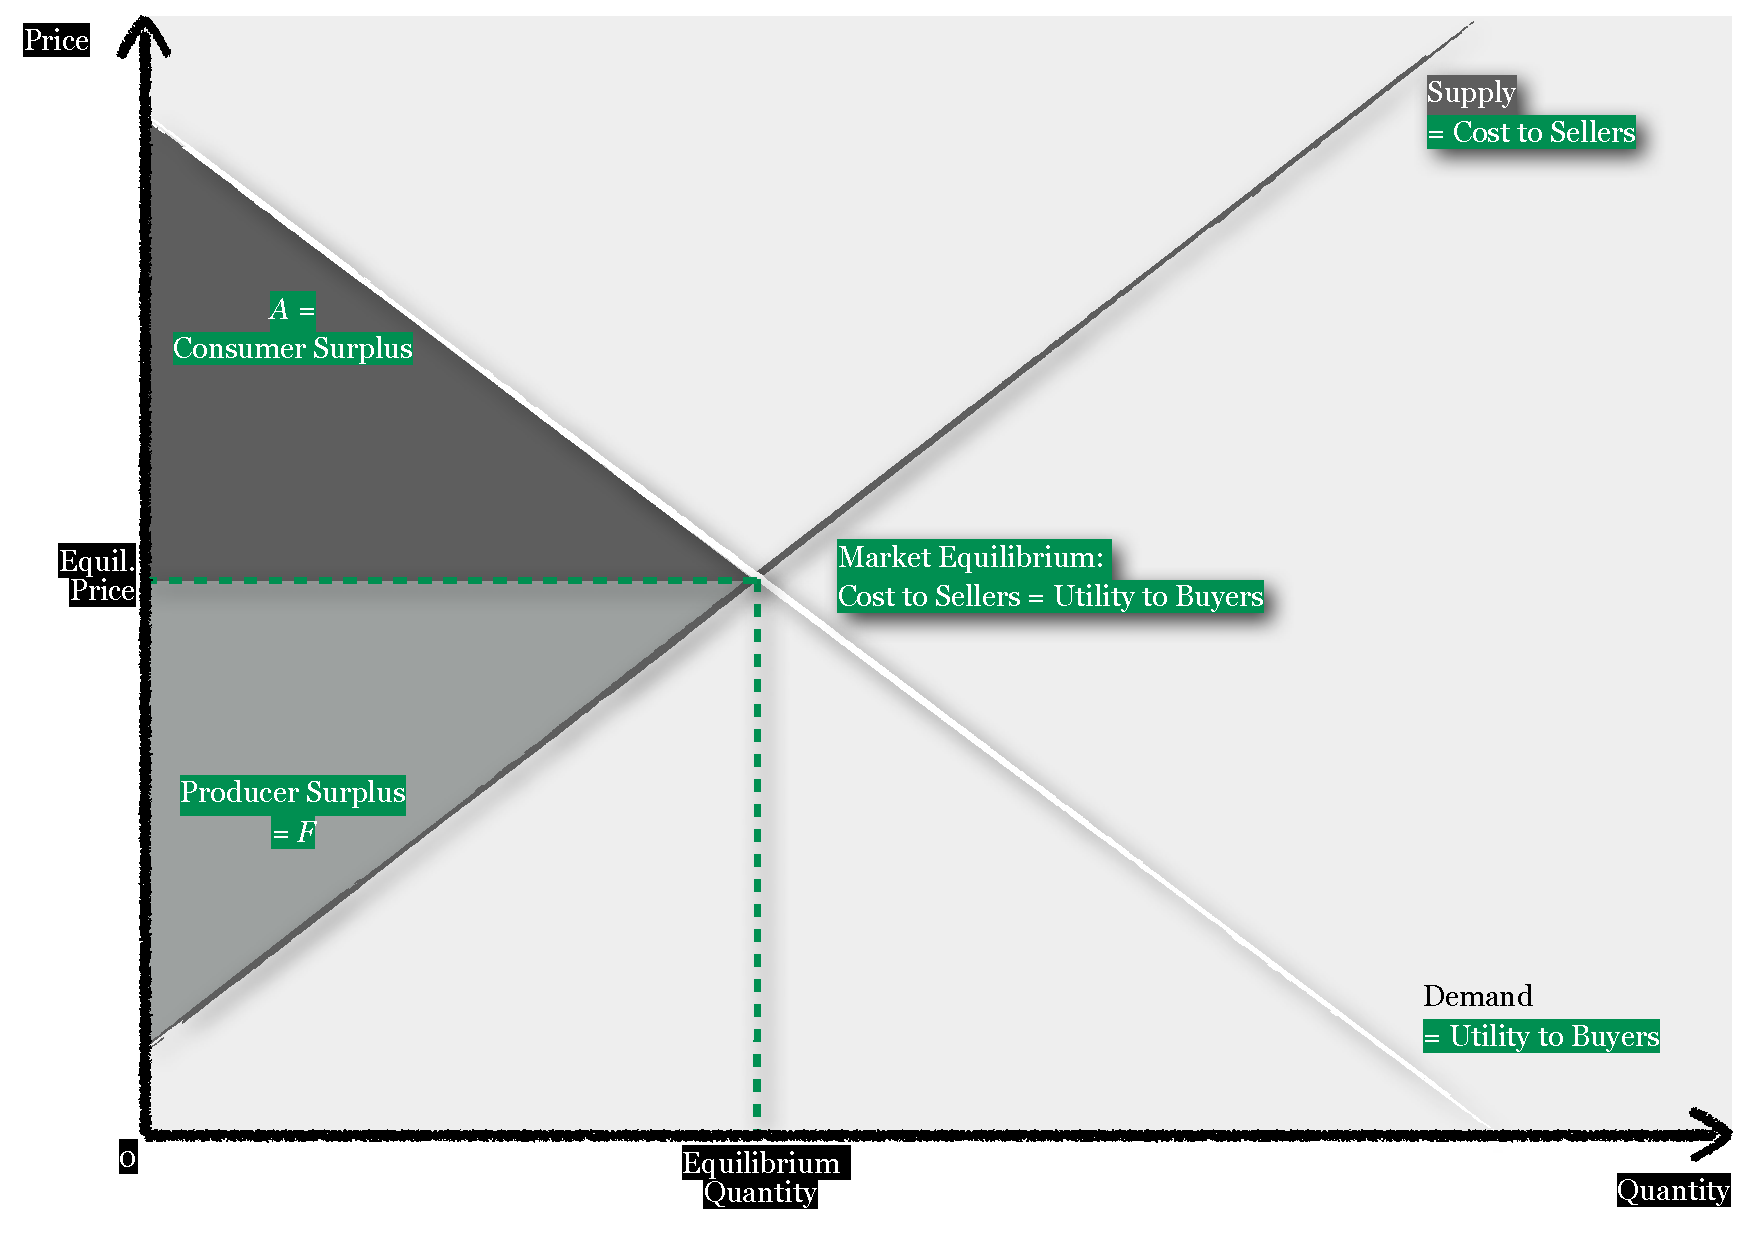
\includegraphics[width=1\textwidth]{supply-demand}
		\caption{Market Equilibrium of Supply and Demand}
		\label{fig:supply-demand}
	\end{figure}

	\item
		The \emph{price system} (see column 1, row 4 in \autoref{tab:ends-mixed-economy}, p.~\pageref{tab:ends-mixed-economy}) makes markets into supreme ``information processors'' \citep{Hayek1931}.
		\footnote{
			Nassim Nicholas \citeauthor{Taleb2007} has recently put this succinctly by praising ``aggressive trial and error'' \citeyearpar[xxi]{Taleb2007} in free markets that ``allow people to be lucky''.
			Being a quantitative trader by profession, \citeauthor{Taleb2007} abandons rational choice when faulting Karl \citeauthor{Marx-1867-aa} \emph{and} Adam \citeauthor{Smith-1776-lq} for believing that free markets work because of \emph{rewards}.
		}
		Because decisions are decentralized, markets can elegantly aggregate dispersed information where a central planner would have to gather them by bureaucratic means (such as a \gls{CBA}).
		Because market decisions are always backed by private costs, the market price system can reveal and communicate (some!) private information, where a central planner may face distorted (inflated) information about cost and utility.
		%smith has referred to this difference as total demand (not backed by money), effective demand (backed by money) this is via prof rae.
\end{enumerate}

\subparagraph[Perfect Competition]{Conditions for Perfect Competition.} \label{sec:perfect-competition}
The above properties of market equilibria hold only under the strict assumptions of perfect or atomistic competition.
In one formulation, this entails \citep[157f.]{McDowell2006}:
\begin{enumerate}
	\item \emph{Infinite buyers and sellers}.
\label{itm:infinite-buyers-sellers}
		There are so many consumers and producers in the market that an offer or bid by any one of them will have a negligible impact on prices.
		Everyone is a price taker.
	\item \emph{Zero barriers to entry and exit}.
\label{itm:easy-entry-exit}
	 	Firms can start or cease to produce a good at relatively little cost and effort.
	 	All markets are wide open.
	\item \emph{Perfect factor mobility.} \label{itm:perfect-factor-mobility}
		In the long run, labor, capital and other inputs to production can move to wherever they earn the highest rents.
		It is hire and fire.
	\item \emph{Perfect information}.
\label{itm:perfect-information}
		Consumers know all prices and qualities of goods, producers know all prices and qualities of factor inputs.
		People are omniscient and powerful calculators of utility.
	\item \emph{Profit-maximizing firms}.
\label{itm:profit-maximizing-firms}
		Firms sell at the price and quantity that maximizes their profit.
		\footnote{
			\citeauthor{Friedman1970a}'s dictum applies:
			``The Social Responsibility of Business is to Increase its Profits'' \citeyearpar{Friedman1970a}, both as commandment and promised salvation.
		}
		Other, exogenous criteria are not part of firm decision making.
Given the other assumptions of perfect competition, firms sell where marginal cost equals marginal revenue.
		\footnote{
			This assumption is politically consequential.
			If firms and their owners, in fact, merely maximized their profits, their property would \emph{not} bestow power.
			By definition, to be a profit-maximizer in a competitive market is to \emph{only} do things that pareto-improve everyone over a given distribution.
			For property to bestow power in the classic definition \citep[8ff]{Geoff2002}, owners must sacrifice some of their profit to make other people do something they would \emph{not} otherwise (pareto-optimally) have done.
			Under microeconomic dictum, owners exert power by \emph{transferring} or \emph{relinquishing} some of their surplus production.

			Clearly, to assume profit maximization and thereby to effectively define away a power aspect of property is implausible, and it rests on some heroic assumptions of human rationality and utility-maximization.
			More importantly, profit maximization implies --- as all such static microeconomics --- that future profits, and thereby, future demand \emph{can} be known, at least probabilistically.
			From a more dynamic or evolutionary perspective, capitalism is \emph{path dependent}, and those rich enough to bet on future profits now will make the very paths on which that future depends.

			Property \emph{does} bestow power, and the kind of axiomatical contortions to define that away probably constitute the kind of hegemonic tendencies of microeconomic thinking that so (rightly) infuriates its critics.
			However, any emancipatory or equity argument on the distribution of property should explicate its relaxation of profit maximization, and provide some preliminary account of the motivations of rich people, instead.

			I take up this argument when I discuss the \hyperref{sec:tax-justice}[fairness of taxation] (p.~\pageref{sec:tax-justice}), especially of a \glsfirst{WT}.
		}

	\item \emph{Homogeneous products.}\label{itm:homogeneous-products}
		Goods produced by one supplier are the same as those produced by another supplier of the same category.
		Inputs provided by one factor owner are the same as those provided by another owner of the same factor.
		All goods and factor inputs are completely commodified.
\end{enumerate}

To this, one might add, according to \citeauthor{Wikipedia2012}:
\begin{enumerate} \setcounter{enumi}{6}
	\item \emph{Zero transaction costs.} \label{itm:zero-transaction-costs}
		Buyers and sellers can exchange goods, services and make contracts at zero cost.
		Search, information, bargaining, policing and enforcement costs are assumed away.
		There is no friction.
	\item \emph{Constant returns to scale.} \label{itm:constant-returns-to-scale}
		For any additional unit produced, costs rise by the same amount, no matter how much units are produced.
		The cost function is \emph{linear}, marginal costs are constant.
		There are no (dis)economies of scale or scope.
		\footnote{
			Constant returns to scale contrast with the very idea of functional differentiation, economic modernization and division of labor discussed \hyperref[sec:modernity]{earlier} (p.~\pageref{sec:modernity}) and \hyperref[sec:growth-solidarity]{later} (p.~\pageref{sec:growth-solidarity}).
		}

		Constant returns to scale are related to, but distinct from assumption \ref{itm:easy-entry-exit} on \hyperref[itm:easy-entry-exit]{easy entry and exit}.
		Excessive economies of scale imply difficult entry.
		Conversely, difficult entry implies varying marginal costs at low output.
	\item \emph{Property rights} \label{itm:property-rights} are well established.
\end{enumerate}

Lastly, --- if somewhat redundant, because axiomatically assumed away by neoclassical welfare economics --- I would add:

\begin{enumerate}\setcounter{enumi}{9}
	\item \emph{Utility equals willingness to pay.} \label{itm:same-budgets}
	The first theorem of welfare economics --- that above specified perfect markets equilibrate at pareto optimality over \emph{initial} distributions --- is often misrepresented to imply that individual \emph{utility} is adequately expressed in willingness to pay, on which free market exchanges operate.
	This shortcut works only under the most heroic assumption of all:
that all market participants have the same budget constraint.

	If everyone invoking the first theorem were to represent it in full, including the crucial, qualifying ``\ldots over \emph{given} allocations'', this condition for perfect competition would be unnecessary.
	Alas, many do not.

	Moreover, equating individual utility with willingness to pay constitutes what might be called the \hyperref[sec:different-budget-constraints]{original, logical sin} of welfare economics (p.~\pageref{sec:different-budget-constraints}, because it \emph{both} assumes equal \emph{and} unequal budget constraints:
the former to maximize utility, and the latter as incentive.
	For a thesis so thoroughly grounded in neoclassical orthodoxy as this, it seems appropriate to feature this contradiction prominently.
\end{enumerate}

I note wherever I relax some of these strict (and rarely plausible) assumptions in the following sections (summarized in \autoref{tab:assumptions-failures}, p.~\pageref{tab:assumptions-failures}).

It should be clear then that I make the above, conservative or neoclassical assumptions less out of conviction, but for their logical elegance and to ``economize on moral disagreement'', as \cite[K226]{GutmannThompson-2004-aa} have suggested.
I hope these positions will be widely acceptable to readers on the political right, and provisionally tolerable to readers on the left.
If I can show taxation to be wasteful, unfair and unsustainable and democracy to be outmatched, assuming even such liberal orthodoxy, sweeping reform should be all the more obvious.

	%!TEX root=../tax-democracy-held.tex

\begin{landscape}
\begin{table}
	\caption[Perfect Competition, Homo Economicus and Corresponding Market Failures]{Relaxing Assumptions about Perfect Competition and Homo Economicus and Corresponding Market Failures}
	\label{tab:assumptions-failures}
	\scriptsize
	\begin{center}
	\begin{tabular}{m{0.36\textwidth}*{10}{m{0.058\textwidth}}*{3}{m{0.09\textwidth}}}
		\toprule
		 & \multicolumn{10}{c}{\hyperref[sec:perfect-competition]{Perfect Competition Assumption} (p.~\pageref{sec:perfect-competition})} & \multicolumn{3}{c}{Homo Economicus}\\
		& %0
		\ref{itm:infinite-buyers-sellers} & %1
		\ref{itm:easy-entry-exit} & %2
		\ref{itm:perfect-factor-mobility} & %3
		\ref{itm:perfect-information} & %4
		\ref{itm:profit-maximizing-firms} & %5
		\ref{itm:homogeneous-products} & %6
		\ref{itm:zero-transaction-costs} & %7
		\ref{itm:constant-returns-to-scale} & %8
		\ref{itm:property-rights} & %9
		\ref{itm:same-budgets} & %10
		Indi-vidually & %11
		Rational &  %12
		Utility-Maximizer  \\ %13

		& %0
		p.~\pageref{itm:infinite-buyers-sellers} & %1
		p.~\pageref{itm:easy-entry-exit} & %2
		p.~\pageref{itm:perfect-factor-mobility} & %3
		p.~\pageref{itm:perfect-information} & %4
		p.~\pageref{itm:profit-maximizing-firms} & %5
		p.~\pageref{itm:homogeneous-products} & %6
		p.~\pageref{itm:zero-transaction-costs} & %7
		p.~\pageref{itm:constant-returns-to-scale} & %8
		p.~\pageref{itm:property-rights} & %9
		p.~\pageref{itm:same-budgets} & %10
		? & %11
		?  & %12
		?  \\ %13

		\midrule
		\hyperref[sec:public-good]{Public good} (p.~\pageref{sec:public-good}) & & & & & & & &X &X & &? & & \\

		\hyperref[sec:common-good]{Common good} (p.~\pageref{sec:common-good}) & & & & & & &X & &X & &? & & \\

		\hyperref[sec:natural-monopoly]{(Natural) market power} (p.~\pageref{sec:natural-monopoly}) &X &X & & & &X & &X & & & & & \\

		\hyperref[sec:principal-agent-problem]{Principal-agent problem} (p.~\pageref{sec:principal-agent-problem}) & & & &X & &X &X & & & & & & \\

		\hyperref[sec:adverse-selection]{Adverse selection} (p.~\pageref{sec:asymmetric-information}) & & & &X & &X & & & & & & & \\

		\hyperref[sec:moral-hazard]{Moral hazard} (p.~\pageref{sec:asymmetric-information}) & & & &X & & & & & & & & & \\

		\hyperref[sec:efficiency-wages]{Efficiency wages} (p.~\pageref{sec:efficiency-wages}) & & & &X & &X &X & & & & & & \\

		\hyperref[sec:winner-take-all]{Winner-take-all} (p.~\pageref{sec:winner-take-all}) & &X & & & & & &X & & & & & \\

		\hyperref[sec:different-budget-constraints]{Different budget constraints} (p.~\pageref{sec:different-budget-constraints}) & & & & & & & & & &X & & &? \\

		\hyperref[sec:diminishing-marginal-utility]{Diminishing marginal utility} (p.~\pageref{sec:diminishing-marginal-utility}) & & & & & & & &X & &? & & &? \\

		\hyperref[sec:monopsony-employers]{(Employer) market power} (p.~\pageref{sec:monopsony-employers}) &X &X &X & & & & &X & & & & & \\

		\hyperref[sec:positional-race]{Positional externality} (p.~\pageref{sec:positional-race}) & & & & & & & & &X & &X & &X \\

		\hyperref[sec:short-term-inconsistency]{Business cycle} (p.~\pageref{sec:short-term-inconsistency})& & & & & & & & & & & &? & \\

		\hyperref[sec:short-term-inconsistency]{Bubbles \& panics} (p.~\pageref{sec:short-term-inconsistency}) & & & & & & & & & & &? &? & \\

		\hyperref[sec:short-term-inconsistency]{De-/Inflation} (p.~\pageref{sec:short-term-inconsistency}) & & & & & & & & & & & &X & \\

		\hyperref[sec:long-term-inconsistency]{Undersaving Commons} (p.~\pageref{sec:long-term-inconsistency}) & & & & & & & & &X & &? & \\

		\hyperref[itm:absolute-advantage]{No trade for some} (p.~\pageref{itm:absolute-advantage}) & & &X & & & & & & & & & & \\

		\hyperref[itm:comparative-advantage]{Different terms of trade} (p.~\pageref{itm:comparative-advantage}) & & &X & & & & & & & & & & \\

		\hyperref[itm:FPE]{Factor price equalization} (p.~\pageref{itm:FPE}) & & &! & & & & & & & & & & \\

		\hyperref[itm:NTT]{Agglomeration} (p.~\pageref{itm:NTT}) &? &? &? & & & & &X & & & & & \\

		\midrule
			& %0
			\tiny \hyperref[itm:infinite-buyers-sellers]{Infinite buyers \& sellers} & %1
			\tiny \hyperref[itm:easy-entry-exit]{Easy entry \& exit} & %2
 			\tiny \hyperref[itm:perfect-factor-mobility]{Perfect factor mobility} & %3
			\tiny \hyperref[itm:perfect-information]{Perfect information} & %4
			\tiny \hyperref[itm:profit-maximizing-firms]{Profit maximization} & %5
			\tiny \hyperref[itm:homogeneous-products]{Homo-geneous products} & %6
			\tiny \hyperref[itm:zero-transaction-costs]{Zero transaction costs} & %7
			\tiny \hyperref[itm:constant-returns-to-scale]{Const. return to scale} & %8
			\tiny \hyperref[itm:property-rights]{Property rights} & %9
			\tiny \hyperref[itm:same-budgets]{Same budget constraints} &%10
			\tiny Indi-vidually & %11
			\tiny Rational &  %12
			\tiny Utility-Maximizer  \\ %13
		\bottomrule
	\end{tabular}
	\end{center}
\end{table}
\end{landscape}


\paragraph{Market Failures.} \phantomsection \label{sec:market-failures}
Markets operate efficiently on private goods:
people can be \emph{excluded} from their \emph{rival} use (see \autoref{tab:types-of-goods}).
In this case, social costs and utility match private cost and utility.

From some goods, people cannot be effectively excluded and/or are not rivals in their consumption.
\footnote{
	I discuss only a popular subset of market failures in this paper.
	I ignore many of the problems recently highlighted by the 2007ff financial and sovereign debt crises.
	While common and public good failures explain much (for example herding and information spill-overs in \citealt{Banerjee-1992-aa}), the 2007ff crises require a dedicated first-order theory of financial capitalism, including an in-depth appreciation of its institutions (for example, derivatives), practices (for example, bank equity) and policies (for example, interest rate).
	\cite{Cassidy2010} provides an equally accessible and comprehensive account of ``How [financial] Markets Fail''.
	%In search for a first-order theory, I review this work elsewhere to tell apart ``The Baby, The Bathwater and the Bathtub'' \citep{Held2012}.}.
}

In these cases, social and private costs and utility diverge and markets may fail.
Goods are overproduced when social cost is higher than private cost (\emph{negative externality}), and goods are underproduced when social benefit is higher than private benefit (\emph{positive externality}).
This problem holds more broadly for \emph{public goods}, \emph{common goods} and \emph{natural monopolies} (see column 1, row 5 in \autoref{tab:ends-mixed-economy}),
\footnote{
	Providing a public good has a positive externality, using a common good has a negative externality.
	Underproviding a public good and overusing a common good can also be represented as \glspl{PD}, where underprovision or overuse is the Nash Equilibrium.

	Whoever first buys a natural monopoly at very high marginal cost, extends the positive externality of very low marginal costs to all subsequent buyers.
}
summarized in \autoref{tab:types-of-goods} according to \citeauthor{Samuelson-1954-eu}'s typology of goods \citeyearpar{Samuelson-1954-eu}.

%!TEX root=../tax-democracy-held.tex

\begin{table}
	\caption{A Typology of Goods}
	\label{tab:types-of-goods}
	\small
	\begin{center}
	\begin{tabular}{lcc}
		\toprule 
		 & \emph{Exclusive} & \emph{Non-Exclusive}\\
		\midrule
		\multirow{2}{*}{\emph{Rival}} & Private Good	 & \hyperref[sec:common-good]{Common Good}\\
						& (Apple)			& (Clean Air)\\[10pt]
		\multirow{2}{*}{\emph{Non-Rival}} & Natural Monopoly\footnote{Often known as a \emph{club good}.} & \hyperref[sec:public-good]{Public Good}\\
								& (Cable TV)				& (Defense)\\
		\bottomrule
	\end{tabular}
	\end{center}
\end{table}%see if both Natural Monopoly and Club good work

\subparagraph{Failure:\ Public Goods} \phantomsection \label{sec:public-good} are \emph{underprovided} by markets, because no one can be prevented from using them (non-exclusion), and they do not get used up (non-rivalry).
Potential buyers can always free-ride on other's purchase and are therefore unwilling to pay producers adequately.
Defense is a public good and fireworks are canonical examples of public goods.

\subparagraph{Failure:\ Common Goods} \phantomsection \label{sec:common-good} are \emph{overused} on markets, because they are rival but again, no one can be prevented from using them \citep{Hardin-1968-aa}.
Potential buyers can free-ride without paying the adequate price for exploiting the rival commons \citep{Hardin-1968-aa}.
\footnote{
	Elinor \cite{Ostrom1990} criticizes the canonically assumed failure of commons in social science and provides an empirically grounded account of their successful, non-coercive governing.
}
\footnote{
	Public and common goods are often hard to distinguish in public choice.
	\emph{Not} overusing a common good is a public good, and providing a public good is a common good.
}
Clean air is a common good, and so may be the enlightened understanding of the electorate \citep{Caplan2007}.

\subparagraph{Failure:\ Natural Monopolies} \phantomsection \label{sec:natural-monopoly}
arise where economies of scale abound in the production or distribution of goods or services, such that only a single or very few suppliers can profitably exist.
Natural monopolies are \emph{mispriced at the margin} because after initial fixed costs --- which few single consumers would be willing or able to pay --- marginal cost become negligible.

Excessive economies of scale often occur in businesses dominated by fixed, rather than variable cost.
Sewer systems, electricity grids or search engines can be natural monopolies with prohibitively high entry costs
\footnote{
	This relaxes the perfect competition assumption \ref{itm:easy-entry-exit} on \hyperref[itm:easy-entry-exit]{easy entry and easy exit}.
}
for basic infrastructure (sewers, electricity masts, web indices) and later, negligibly small marginal costs for adding an additional consumer.
Natural monopolies can incur welfare losses in two ways:
\begin{enumerate}
	\item If only one market supplier exists, it may charge monopoly prices causing a deadweight loss of underconsumption.
	\item In the extreme, given the high marginal cost for the first buyer, no first buyer may come forth and the otherwise
	\footnote{
		Otherwise, if \emph{all} buyers could pay for the initial costs equally.
	}
	pareto-improving natural monopoly may not be provided at all.
\end{enumerate}

\subparagraph[Failure:\ Principal-Agent Problems]{Failure:\ Principal-Agent Problems.}\phantomsection \label{sec:principal-agent-problem}
Principal-agent problems are one market failure of the broader class of information asymmetry problems (row 5, column 2 in \autoref{tab:ends-mixed-economy}, p.~\pageref{tab:ends-mixed-economy}), where at least one party to a trade knows less about the service, good or risk being exchanged (pioneered by Nobel laureates \citealt{Akerlof-1970-aa}, Stiglitz \citeyear{Stiglitz1976} and \citealt{Spence1974}).

In principal-agent problems, the asymmetrically known quality is the effort exerted by the agent on behalf of the principal.
When agent (say, manager) effort cannot be fully observed by principals (say, owners), and principals have interests (say, long-term returns) diverging from those of agents (say, a pet project), agents may be able to cheat on their contracts.
When agents shirk successfully, they will exert less (or ill-directed) effort than would be pareto-optimal.
In the extreme, the market between principals and agents breaks down completely, as principals anticipate shirking agents and forego the transaction altogether.

Applied game theory and related disciplines offer a host of incentive designs to realign interests of principals and agents, which I need not discuss here comprehensively (but see \citealt{Tirole2006}).
Solutions include \hyperref[sec:efficiency-wages]{efficiency wages} (p.~\pageref{sec:efficiency-wages}) --- which creates unemployment --- or deferred compensation and tournaments --- which invites risk-seeking (Holt 1995).
Efficiency wages and tournaments try to alter the probabilistic calculus of would-be shirkers by promising outsized instead of \emph{marginal} rewards and punishment for whichever effort \emph{is} (randomly) observed.
Deferring (part of) the compensation to later may make agents more far-sighted, but will still strictly cap their downside risk, especially when only bonuses are deferred (for example, stock options).
The worst that can happen to an agent in any of these schemes is to loose their job, the tournament promotion or their bonus.
By contrast, the worst that can happen to a principal, is to lose everything.

In addition, if the observations of effort on which such schemes are based are spotty or isolated --- as they often are --- agents can ``game the system'' and incentives may turn ineffective, or even perverse.

Both \hyperref[sec:efficiency-wages]{efficiency wages} (p.~\pageref{sec:efficiency-wages}) and tournament compensation also increase economic inequality:
instead of marginal productivity, they reward \hyperref[sec:winner-take-all]{winners with all}  (p.~\pageref{sec:winner-take-all}) and threaten losers with unemployment.

All these incentive design schemes fall short of the one genuine solution to realign principal and agent interests:
to either sell agents stock or charge them a substantial sign-up fee \citep{Tirole2006}, effectively making agents into principals, too.
Only then can they bear both the full upside and downside risk of the enterprise.
To be able to take on such risk, of course, agents must own substantial assets, which they may not have in an unequal economy.

Principal-agent problems fail markets if, and to the extent that, inequality in assets prevents people from taking equal risks in otherwise welfare-enhancing joint projects.
They are one of the cases, where inequity makes for inefficiency, too.
%add broader reference, idea

This is not merely a theoretical conumdrum, but a very real problem for postindustrial  and knowledge-based economies (for example, Lisbon Strategy, EU 2020, \citealt{Bell-1973-aa}).
\footnote{
	Calls for more startups, patents and research spin-offs, particularly in Germany, may serve as evidence for suboptimal incentive design under the status quo.
}
Almost by definition, an economy based on knowledge and innovation will display information asymmetries.
The effort a knowledge worker (say, a programmer) puts in, cannot easily be observed, because that would require the principal to acquire the exact same specialized knowledge (say, a programming language).
Similarly, a would-be innovator (say, an \gls{ICT} entrepreneur) will always know more about her nascent and uncertain innovation than any possible investor, because otherwise, the investor would have done the project herself, already.

In short, for competitive markets to do their magical ``stochastic tinkering'' \citep[211]{Taleb2007}, people need to be equipped and incentivized to act on their local and uncertain ideas, and to specialize.
For a \emph{homo economicus} at least, there can be no \emph{entrepreneurship} without some \emph{ownership}, too.

%add desideratum here?

\paragraph{State Responses to Market Failures} \phantomsection \label{sec:state-responses}
States can respond to market failures by fiscal and regulatory interventions.
I discuss them for each type of good (rows 6--8, column 1 in \autoref{tab:ends-mixed-economy}).

\subparagraph{Fixing Public Goods.} \phantomsection \label{sec:public-good-response}
States can step in to \emph{provide public goods} or subsidize their private provision, both out of the public purse (fiscal policy).
There is no regulatory or monetary response to public goods failure.
\footnote{
	\label{fn:monetary-commons}
	There are no monetary responses to any of these market failures, because \hyperref[sec:monetary]{monetary policy} (p.~\pageref{sec:monetary}) boosts or retards economic activity \emph{overall} by extending or restricting credit and money creation.
	Markets fail in the provision of public goods, common goods and natural monopolies because these goods are ill-priced \emph{relative} to other goods in the economy.
	States cannot deliberatively correct relative prices in the economy by monetary policy.

	Inflation, if and to the extent that it is caused by monetary overexpansion, may, however appear first in some goods, including long-term assets such as real estate, as appears to have happened in the US monetary expansion up until the 2007ff financial crisis.
	%add reference
	These relative price changes on the first impact of inflation cannot be effectively targeted by government and eventually propagate into an overall increase in price levels.
	%add reference
}

\subparagraph{Fixing Common Goods.} \phantomsection \label{sec:common-good-response}
States can protect overused commons by a regulatory policy of ``fencing in the commons''.
\footnote{
	The expression stems from Ireland, where the British king passed enclosure legislation to privatize and built fences around previously communal pastures.
	%reference!
}
By doing so, governments follow the \cite{Coase1960} theorem.
It holds that markets can pareto-optimally resolve externalities if transaction costs are sufficiently low, and if property rights are well-defined.
\footnote{
	The Coase theorem further holds that it does not matter to whom the property rights are initially granted, say whether the polluters are granted a right to pollute, or citizens are granted a right to clean air (invariance thesis).
	While \emph{welfare} neutral, this original granting of property rights does have distributive effects:
	whoever is granted the property right, enjoys a windfall.
	Economists often suggest to auction off new property rights at competitive prices, to minimize arbitrary distributive effects.%missing source
}
The Coase theorem is often erroneously cited to argue against state intervention.
Maintaining and \emph{issuing new property rights} are, of course, \emph{regulatory} state interventions.
\footnote{
	Here's what happens upon privatization:
	Enclosed public goods become natural monopolies.
	Enclosed common goods become private goods, as per \autoref{tab:types-of-goods} (p.~\pageref{tab:types-of-goods}.
}

Alternatively, states can resolve ``Tragedies of the Commons'' \citep{Hardin-1968-aa} fiscally by slapping a \emph{Pigouvian tax} (\citealt{Pigou1912}, popularized by \citealt{Baumol1972}) on using the commons.
\footnote{
	States can also regulate common goods by outlawing its overuse, as the US does by instituting minimum \gls{CAFE} standards on automakers.
	Regulation by defining maximum acceptable use of commons is inefficient, because it does not incentivize market participants to save the commons wherever it is marginally cheapest to do so.
	Standards regulation cause a \gls{DWL} much like minimum wages or other price floors and ceilings.
}
The Pigouvian tax prices in the externality of using a common good.
\footnote{
	The German term for a Pigouvian tax, helpfully, translates to ``steering tax'' (Lenkungssteuer).
}

There is no monetary response to overused commons (see \autoref{fn:monetary-commons}, p.~\pageref{fn:monetary-commons}).

\subparagraph{Fixing Natural Monopolies.} \phantomsection \label{sec:natural-monopoly-response}
Governments can avoid the deadweight losses of natural monopolies fiscally, by nationalizing them (for example, public ownership of motorways in Germany) and ideally charging users a fee at \emph{average} cost (for example, trucks and coaches on federal motorways in Germany).
\footnote{
	\label{fn:why-ac-fees}
	Recall that prohibitevely high initial marginal cost marred private markets in the first place.
}
Governments can also procure natural monopoly goods and services from private firms and charge users a fee at average cost (for example, local railway in Germany).

%%%%%%%%%%%%%%%%%
% I have cleaned up, revised the document until here!
%%%%%%%%%%%%%%%%%

Alternatively, governments can allow privately held natural monopolies but tightly regulate them to enforce pricing at average cost and avoid a monopoly \gls{DWL} (for example, \emph{last mile} \gls{ICT} or electricity in Germany).

There is no monetary response to natural monopoly problems (see footnote \ref{fn:monetary-commons}).

%\subparagraph{Fixing PCA-Problems}
%\subparagraph{Entrepreneurship Needs Broad-Based Ownership.} \phantomsection \label{sec:Ownership} More deductively, market economies can be thought of as welfare-maximizing because they capture decentralized and/or privately known information, and let diverse solutions compete.
%Nassim Nicholas \cite{Taleb2007} has put this succinctly by praising ``aggressive trial and error'' (\emph{ibid.}:
%xxi) in free markets that ``allow people to be lucky'' (\emph{ibid.}:
%xxi)\footnote{Being a quantitative trader by profession, \cite{Taleb2007} actually abandons rational choice when faulting Karl \cite{Marx-1867-aa} and Adam \cite{Smith-1776-lq} for believing that free markets work because of rewards.}.
%This basic impetus for capitalist creativity is expressed in desideratum \ref{des:Entrepreneurship}:

%\begin{desideratum}[Entrepreneurship]
%	A desirable tax will allow entrepreneurs to make their own production decisions according to their independent judgement of private and/or local information.
%	\label{des:Entrepreneurship}
%\end{desideratum}

%But what is required for this ``stochastic tinkering'' (\citealt{Taleb2007}:
%211) to work?

%Principal-agent theory suggests that maximum effort may not be exercised when effort of agents is imperfectly or non-observable, or other information asymmetries prevail.
%This of course --- unobservable effort and information asymmetries --- are likely features of highly differentiated knowledge economies\footnote{Calls for more startups, patents and research spin-offs, particularly in Germany, may serve as evidence for suboptimal incentive design under the status quo.}, where people produce an idea, not a piece of welded metal (cf.~\citealt{Bell-1973-aa}).
%Game theoretic incentive design suggests that information asymmetry problems can be resolved either by making agents shareholders or by charging them substantial sign-up fees, both of which require substantial assets to begin with \citep{Tirole2006}.

%In short, for competitive markets to work their magic, people need to be equipped and incentivized to act on their local and diverse ideas.
%For \emph{homo economicus}, there can be no \hyperref[des:Entrepreneurship]{entrepreneurship} without some \hyperref[des:BroadOwnership]{ownership}, too.

%This ties in with the simple capitalism desideratum presented earlier, but it also adds a specification:

%\begin{desideratum}[Broad-Based Ownership]
%	A desirable tax allows for or promotes a broad-based ownership of the means of production.
%	\label{des:BroadOwnership}
%\end{desideratum}

%include footnote for all desideratum's of where they are leading.
%reference the same footnote

%\subsection[Welfare Gains]{Welfare Gains:
%How Taxes Can Make the Pie Larger} \label{sec:PurposesOfTaxation}
%The burden of proof is on the state for interventions in the market.
%Witnesses for the defense are summarized in \autoref{tab:ends-mixed-economy} and are entertained in the below.

%Taxes and other state interventions in the economy can in fact enhance market outcomes in several ways:

%this figure is obsolete, it is now \label{tab:ends-mixed-economy}

%\begin{description}
%	\item[Redistribution.] \phantomsection \label{sec:Redistribution} Governments may respond to excessive \emph{inequality} by taxing people proportionally or progressively to redistribute resources.
%While inequality is further discussed in \autoref{sec:Equity} on \hyperref[sec:Equity]{equity}, it does bear on efficiency, too, as is argued in \autoref{sec:InequalityIsInefficient}.

%	\item[Risk Pooling.] \phantomsection \label{sec:RiskPooling} People can possess \emph{asymmetric information} about things of uncertain quality they exchange on the marketplace.
%Insurance of unemployment, health or disability are principal examples, where sellers of risk (insurants) typically know more about their own risks than buyers of risk (insurers)\footnote{This relaxes perfect competition condition {itm:PerfectInformation} (\hyperref[itm:PerfectInformation]{perfect information}).}.
%Less-informed buyers (insurers) of risks may expect bad risks for \emph{all} insurants, causing premiums to rise and driving low-risk sellers out of the market entirely.
%This mechanism may repeat until no exchanges are made at all, defeating the purpose of insurance.

%	Governments can avoid these \emph{lemons markets} by forcing everyone to take out insurance \citep{Akerlof-1970-aa}.
%When risks are universal --- as is arguably the case for unemployment, health and disability --- the premiums for these insurances are effectively taxes.

%	\item[Public Goods] \phantomsection \label{sec:PublicGood} can be enjoyed by an arbitrary number of people without exhaustion (non-rivalrous) and no one can be excluded (non-excludable) from its using (\citealt{Samuelson-1954-eu}, summarized in \autoref{tab:Types-Of-Goods}).
%National defense is one example.
%Because people in larger groups can always free-ride on the provision of public goods by others, they are likely to be \emph{underprovided} by self-seeking individuals or markets \citep{Olson-1971-aa}.

%	Governments can improve welfare by providing public goods out of tax revenue.

	%the types of good table happens earlier, as 	\label{tab:types-of-goods}

%	\item[Common Goods] \phantomsection \label{sec:CommonGood}  are rival in their consumption but do not allow exclusion:
%everyone can benefit, but they can be exhausted \citep{Samuelson-1954-eu}.
%A \emph{Tragedy of the Commons} occurs when people overuse the common good \citep{Hardin-1968-aa}\footnote{Elinor \cite{Ostrom1990} criticizes the canonically assumed failure of commons in social science and provides an empirically grounded account of their successful, non-coercive governing.}.

%\begin{quote}
%	\emph{What is common to the greatest number has the least care bestowed upon it.}\\*\\*
%	Aristotle, Politics, Book II, Chapter 3 (384 b.c.-322 b.c.)
%\end{quote}

%	Government can avoid the \emph{negative externality} of exhaustion of commons by \emph{pricing in} the costs of its use, an approach also known as Pigouvian taxation (\citealt{Pigou1912}, popularized by \citealt{Baumol1972})\footnote{The alternative, non-tax solution of issuing property rights on the commons (for example through an Emissions Trading Scheme), thereby making it an ordinary private good is of course a ``government'' solution, too.
%Markets cannot maintain, let alone introduce new property rights.}.%check definitively whether it is Pigovian our Pigouvian.
	%note from correction:
%add coase theorem in here.
%Note that some solutions are costly.

%	\item[Natural Monopolies] \phantomsection \label{sec:NaturalMonopolies}  arise where economies of scale abound in the production or distribution of goods or services, such that only a single supplier can profitably exist\footnote{This relaxes perfect competition condition \ref{itm:PriceTakers} (\hyperref[itm:PriceTakers]{price taking}) and {itm:EasyEntry} (\hyperref[itm:EasyEntry]{easy entry and exit}).}.
%Excessive economies of scale often occur in businesses dominated by fixed, rather than variable costs.
%Sewer systems, electricity grids or search engines can be natural monopolies with prohibitively high entry costs for basic infrastructure (sewers, electricity masts, web indices) and later, negligibly small costs for adding an additional consumer.
% Natural monopolies can incur welfare losses in two ways:
%if only one market supplier exists, it may charge monopoly prices causing a deadweight loss of underconsumption.
%Conversely, if several suppliers exist in one market, each of them may be unable to invest at optimal levels (underprovision).
%%This ain't quite right.
%I'm missing the marginal vs.\ average cost problem.

%	Governments can avoid the deadweight losses of natural monopolies by regulating them (for example, last mile ICT in Germany), franchising or outsourcing them (for example, local railway in Germany), enforcing common carriage (for example, electricity in Germany) or by nationalizing them (for example, public ownership of motorways in Germany).

%	\item[Easy Market Entry.] Problems of prohibitive entry costs are not limited to natural monopolies\footnote{This relaxes perfect competition condition {itm:EasyEntry} (\hyperref[itm:EasyEntry]{easy entry and exit}).}.
%Competition can also be hampered by market players who enjoy excessive economies of scale by sheer size or past learning curves.
%Aside from regulatory responses (antitrust), governments can react proactively by means of infant industry protection or other industrial policy, the contested (de)merits of which are not under further consideration here\footnote{If infant industry protection \emph{is} considered welfare-enhancing, its medium-term welfare losses to the polity (either in the form of a DWL of subsidizing or protectionism) become a public good to the extent that a successful infant industry generates positive externalities for the  rest of the economy.
%As such, infant industry protection should be partially financed out of general revenue.}.
%\end{description}

\paragraph{Monetary Policy for Price Stability.} \phantomsection \label{sec:price-stability} Monetary policy contributes best to efficient production --- and almost\
footnote{
	Except for \nameref{sec:monetary-stimulus} (p.~\pageref{sec:monetary-stimulus}).
}
all other dimensions of material human need --- by staying out of the way of markets with stable prices
\footnote{
	For two technical reasons, most economists and central banks prefer a positive, but moderate and stable rate of inflation of around 2\% rather than perfect price stability at 0\% inflation:
	\begin{enumerate}
		\item A positive inflation rate gives central banks room for maneuvre in fiscal stimulus.
		At moderate inflation, central banks can pursue a \emph{negative} real interest rate (as was the case in 2011ff in many markets).
		\item A positive inflation rate can mitigate the hypothesized downward stickiness of nominal labor costs.
		Real wages will fall even when nominal wages stay constant.
		%needs sources
	\end{enumerate}
}
to allow efficient exchanges in the first place.
When prices rise (inflation) or fall (deflation) overall, otherwise pareto-optimal exchanges may be hampered.

The welfare losses of inflation include \begin{inparaenum}[\itshape a\upshape)]
	\item hoarding (of real assets),
	\item drowning out relative price changes (noise),
	\item increasing transaction costs (such as shoeleather costs
	\footnote{
		The cost of minimizing cash holdings, including many trips to the bank, during which shoe leather is supposedly worn down.
	}
	and menu costs
	\footnote{
		The costs of repricing for business, including the cost of changing restaurant menus.
	}
	), as well as
	\item general uncertainty and possibly, unrest.
	\end{inparaenum}
Cost-wage spirals
\footnote{
	Experiencing higher consumer prices, workers will demand higher wages, which in turn prompts producers to increase sale prices.
}
make inflation self-reinforcing, potentially escalating into hyperinflation.
Inflation is also believed to set off the business cycle \citep{Friedman1970}.

Deflation, while scarcely observed in the western world in the post-Bretton-Woods regime,
\footnote{
	With the exception of Japan's lost decade.
	%citation needed
}
is similarly damaging.
It also makes \begin{inparaenum}[\itshape 1\upshape)]
	\item transactions more costly and
	\item heightens uncertainty.
Deflation can also
	\item cause the hoarding of cash and
	\item trap liquidity
	\footnote{
		Under deflation, holding (increasingly valuable) cash is relatively more attractive than investing.
	}
	and self-reinforce into a deflationary spiral.
	\end{inparaenum}

In the long run, monetary expansion (or contraction) should follow the output of the economy $G$, so that price levels stay stable.
\footnote{
	This, if nothing else, is the reason why backing a paper currency with specie (such as the Gold standard) or pegging it to another currency (fixed exchange rate) are bad ideas:
	under such fixed or pegged regimes, the money supply expands and contracts \emph{independent} of output.
	Under the gold standard, money supply tracks discovery and extraction of gold --- a process which is likely unrelated to economic output.
	This, in addition to the transaction costly lunacy of digging up gold in one place (a mine) only to bury it in another place (a vault).

	Similarly, under a pegged (or fixed) exchange rate, money supply follows the monetary command of \emph{another} economy.
}

Whether inflation and deflation are, as the monetarists would have it, ``always and everywhere a monetary phenomenon'' \citep{Friedman1970}
%page missing
and therefore caused by an over-expansion or contraction of the money supply in the first place, or whether it has it roots in the real economy as the Keynesians would argue, is a very complicated empirical question but --- luckily for the author --- irrelevant to the state job of ensuring an efficient market place.
No matter ``who dunnit'', monetary policy should aim at price stability, and, perhaps, counteract real price shocks --- if and to the extent that they occur --- with \nameref{sec:monetary-stimulus} (p.~\pageref{sec:monetary-stimulus}.).%this needs to be expanded, verified.

\subsection[Pooled Risks]{Pooled Risks:\ Saving the Pie} \label{sec:risk}
\footnote{
	I concentrate here on \emph{individual} risk.
	Governments and markets should also reduce \emph{aggregate} risk and systemic uncertainty \citep{Knight1921}.
	They should avoid extreme negative risks, seek extreme positive risks \citep{Taleb2007} and avoid systems too complex and tightly coupled to be safely operated by humans \citep{Perrow-1999-aa}.
	To the extent that such precaution, requires fiscal, regulatory or monetary policy intervention, this end also depends on intact \nameref{sec:means} of the mixed economy (p.~\pageref{sec:means}).
}

\paragraph{The Human Condition of Risk.} \phantomsection \label{sec:human-nature-of-risk} Humans inhabit a volatile environment, marred by low probability, but high impact events (\emph{black swans}, according to \citealt{Taleb2007}), for example a serious work accident.
Unfortunately, humans also tend to ignore precisely such low probability, but high impact events \citep{Taleb2007}, and overestimate the probabilities of favorable outcomes \citep[44]{Baron2000}, especially when they have few cognitive resources available.
When they give it some thought, most people \emph{avoid grave downside risks}:
for example, most will prefer the certain but low cost of car liability insurance over the rare but high cost of paying for a car accident (column 2, rows 1--3 in \autoref{tab:ends-mixed-economy}).
\footnote{
	If people were neutral between upside and downside risks, they would be indifferent between a lifetime of car insurance premiums and a (low) probability of accidental personal bankruptcy.
	%citation needed
}

%here are two important notes from prospect theory, and Kahnemann 2012
	%I think insurance requires only the weaker (contested by Kahnemann) expected utility hypothesis (bernoulli), who says that risk aversion can be explained merely by diminishing marginal utility (specifically, argues Bernoulli, utility is a logarithmic function of wealth).
%Maybe I can do here with risk aversion and don't need LOSS aversion (based on reference points), which is what Kahnemann is out to explain, and with him prospect theory.
%Consider a weird graph about that in Kahnemann.
	% The mixed economy can be understood as those institutional crutches that help system-one humans to behave as system-two humans, because system-two can't be relied upon in the long run, it's too effortful to use.
%So we use institutions to get us there -- because system two is the better.
	% Kahnemann raises a big stink with indifference curves:
%he says neoclassical economics is wrong there, because prospect theory shows that people have reference points from which they are loss averse, suggesting that there is no such thing as an indifference curve (I am not sure that is formally right, the indifference curve just wouldn't be linear, as it might be).
	% my problem with Kahnemann is that he meanders between positive and normative theory.
%I would think prospect theory is a positive finding, but it need change normative theory.
%Of course, Kahnemann might say, well if utility is experienced according to prospect theory, than maybe THAT is the kind of utility that we should maximize.
%I disagree:
%I think we should let system two reign, and therefore also need not abandon neoclassical economics, we just must make sure that there is always good and enough crutches around.


\paragraph{Market Solutions to Risk:\ Insurance.} \phantomsection \label{sec:insurance} Markets provide \emph{insurance} as a ready-made institution to address this human need for down-side risk aversion (column 2, row 4).
Insurants can buy protection from their grave downside risk, say, a car crash, by pooling their individual risks.
An insurance deal stipulates that all insurants will regularly chip in a small amount to cover the few unlucky car wreckers, in return for the promise that they, too, will receive a payout if they crash their cars.
\footnote{
	With sophisticated financial markets, insurants buy this protection not just from one another, but also from other (rich) people or financial intermediaries willing to stomach the risk for a premium.
}

Aside from car insurance, markets do sometimes, to some extent, provide insurance against the four big life risks commonly associated with the welfare state:
\begin{inparaenum}[1)]
	\item unemployment,
	\item sickness,
	\item accident and
	\item disability.
	\footnote{
		I do not include old age here, because the risk component (a long life in retirement) of pensions is small compared to the saving component.
		Other insurances, notably health insurance, also include a saving component (for high morbidity in old age), but the risk component dominates.
	}
\end{inparaenum}

Market insurance of these life risks \emph{does not} involve a redistributive component, though that is easily assumed for unemployment insurance.
The \emph{voluntary} exchange of premiums for coverage, in car and all other insurance, is a pareto-improvement:
all risk-averse insurants are better off, by hedging against downside risks.
Insurance is not obligatory and whoever finds it unnecessary (as may be the case for rich individuals who face limited downside risks) is not affected.

\paragraph{Market Failure in Insurance:\ Asymmetric Information.}
\label{sec:asymmetric-information}

Insurance markets may fail when buyers and sellers possess asymmetric information about the risks to be insured.
\footnote{
	This relaxes perfect competition assumption \ref{itm:perfect-information} on \hyperref[itm:perfect-information]{perfect information}.
}

\subparagraph[Adverse Selection]{Ex ante,}\phantomsection \label{sec:adverse-selection} insurants with privately known high risk may disproportionately take out insurance.
Insurers, anticipating such \emph{adverse selection}, but unable to tell high-risk (``lemons'') from low-risk (``cherries'') applicants,
\footnote{
	The conventional terminology stems from \citeauthor{Akerlof-1970-aa}'s original paper, in which he modelled quality uncertainty in the market for used cars.
	In American slang, a lemon is a car ``that is found to be defective only after it has been bought'' (Wikipedia).
	A cherry, conversely, is a good used car.
}
may expect bad risks for \emph{all} buyers, causing premiums to rise and further driving low-risk insurants out of the market.
This \emph{lemons market} mechanism may repeat until no exchanges are made at all, defeating the purpose of insurance \citep{Akerlof-1970-aa}.

Adverse selection abounds in the insurance of the big life risks.
Ex ante, insurants know more about their likelihood to become unemployed, sick, to be in an accident or become disabled than their insurers.
\footnote{
	Prior the Obama administration's \gls{PPACA}, in the US, \emph{pre-existing conditions} were frequently exempted from private health insurance contracts, defeating the purpose of insurance for many chronically ill or disabled persons.
	Private insurers minimize the ex-ante problem of asymmetric information by excluding those risks about which the insurants may already know.

	In Germany, insurants experience a similar frustration if they seek to take out (recently privatized) occupational disablement insurance, facing greatly limited coverage (for example, no cardio-vascular conditions), eligibility (for example, no back-related conditions for construction workers) or premiums (for example, higher rates for burnout-prone teachers).
}

\subparagraph[Moral Hazard]{Ex post,} \phantomsection \label{sec:moral-hazard} sellers of risk (insurants) might take on more risk than they otherwise would have, causing moral hazard and in turn drive up premiums.

Moral hazard, too, may occur in the insurance of big life risks.
Ex post, insurants may be willing to live less healthily, or more recklessly than they would without insurance.

\paragraph{State Responses to Asymmetric Information in Insurance.} \phantomsection \label{sec:state-insurance}

\subparagraph{Ex ante,} states can resolve lemons markets by \emph{regulatory} means if they force everyone at risk to take out insurance (\citealt{Akerlof-1970-aa}, \citealt{Barr})
(column 2, row 8).
\footnote{
	To the extent that government also regulates coverage and admittance, as it would have to do to avoid a lemons markets, the mandatory, nominally private insurance becomes a partly quasi-fiscal institution.
	When central qualities of the products (insurance) are regulated and buyers forced to buy, premiums are to a large extent pre-determined.
	Insurance firms will differ only in the few, administrative components of their business outside the reach of state command.
	The part of the premium that covers the mandated services is effectively a tax, and the insurance company but an outsourced service provider to the government.
	Ignoring, as I have here done, the (vexingly complicated) supply side of medical care, the difference between mandatory private and public health insurance appears small.
}

States can also resolve lemons markets by \emph{providing benefits} out of the treasury (column 2, row 9).
As the risks of unemployment, health, accident and disability are near-universal,
\footnote{
	Even people with a privately known risk of zero should be included, as low-risk insurants may otherwise find it attractive to misrepresent their privately known risks.
	This extreme case of a privately known risk of (close to) zero cannot be justified under an efficiency norm of Pareto optimality, as everyone is made better off by making some people worse off.
	Instead, it requires the stronger Kaldor-Hicks efficiency norm \citep{Kaldor1939,Hicks1939}.
	Resolving a lemons market may cost some people less than it will benefit others.
}
the contributions for such state-run insurance are effectively taxes.
Some states (such as Germany) outsource insurance to quasi-fiscal organizations.
This ``social insurance'' may make a difference in administrative, legal or rhetorical terms, but its economics are that of a state-run insurance and its revenues are taxes.
Financing public insurance out of dedicated ``social contributions'' (usually regressive payroll taxes) instead of general revenue only adds a specific distributive component (a regressive tax on labor) to the overall tax schedule.
\footnote{
	Because \nameref{sec:redistribution-and-revenue-are-one} (p.~\pageref{sec:redistribution-and-revenue-are-one}).
}
\footnote{
	In perfect markets with sufficient price flexibility it also does not matter whether social contributions are levied from employers or employees.
	The incidence of a tax depends only on the relative price elasticity of supply and demand for labor.
	In labor markets, employees (supply) are typically less price elastic than employers (demand) who can substitute labor for capital, or move their capital.
	Employees end up paying for ``social insurance'' no matter the nominal burden.
	Only the \hyperref[sec:well-determined-incidence]{incidence of taxation} matters (p.~\pageref{sec:well-determined-incidence}).
}

Mandating insurance or, equivalently, providing benefits out of the public purse need not redistribute resources over and above the Kaldor-Hicks improvement from resolving a lemons markets.
Properly understood, state interventions to hedge \emph{individual} risks are meant to improve the efficiency, not equity of outcomes.
Real policy often differs from this \hyperref[sec:ordoliberal-hygiene]{ordoliberal ideal} (p.~\pageref{sec:ordoliberal-hygiene}) and layers distributive components on top of the Kaldor-Hicks improvement.
In Germany, for instance, social contributions are proportional, but capped and public health insurance covers an insurant's children at no additional cost.
These additions to schedule and benefits may or may not be desirable, but they properly belong in the realm of \hyperref[sec:distribution]{distributive policy} (p.~\pageref{sec:distribution}).

\subparagraph{Ex post,} states and markets have essentially the same, clumsy method to reduce moral hazard:
\footnote{
	Again, states and markets are not the only way to organise production and distribution of material goods, emphatically not in the mainstays of moral hazard, such as decisions about medical care.
	\cite{Schwartz2010} argue passionately for a patient-doctor relationship based on trust and ``Practical Wisdom'' and cogently argue how \emph{any} system based on incentives can, and \emph{will} be perverted.
}
they re-individualize some of the risk by asking for co-payments or provide incentives for prudent behavior.
Exploiting moral hazard is a \hyperref[sec:common-good]{commons problem} (p.~\pageref{sec:common-good}), and can therefore be resolved either by (partial) property rights (co-payments) or by Pigouvian taxation (incentives).

\subsection[Equitable Distribution]{Equitable Distribution:\ Slicing the Pie Fairly} \label{sec:distribution}

\paragraph{The Human Condition of Inequality} \phantomsection \label{sec:human-nature-of-inequality} Humans, the social animals, can deal with material scarcity in two ways \citep{Pickett-2009-kx}:
\begin{inparaenum}[1)]
	\item ``because members of the same species have the same needs as each other, they have the potential to be each other's worst rival'' \citeyearpar[197]{Pickett-2009-kx} but also,
	\item ``the potential to be each other's best source of cooperation, learning, love and assistance of every kind'' \citeyearpar[198]{Pickett-2009-kx}.
\end{inparaenum}

\begin{description}
	\item[Dominance Strategies.] The first, \citeauthor{Hobbes-1651-aa}ian \citeyearpar{Hobbes-1651-aa}
	strategy is one of dominance:
	\footnote{
		According to \cite{Hobbes-1651-aa} ``life in a state of nature'' would be ``solitary, poor, nasty, brutish and short''.
	}
\emph{homo homini lupus est}, man is a wolf to his fellow man.
Following \emph{dominance strategies} (column 3, row 1 in \autoref{tab:ends-mixed-economy}), humans --- much like their primate cousins, the chimps --- maximize their classical evolutionary fitness (\citealt{Darwin1859}, recently \citealt{Dawkins1976}) by relying on individual power to secure access to scarce resources (food, shelter, females).

	\item[Affiliative Strategies.] The second strategy is one of \emph{affiliation} (column 3, row 3) and mutuality:
	to be your ``brothers keeper'' (\gls{KJV} Bible, Genesis 4:9).
	\footnote{
		Whether a capacity for altruism really developed out of genetic nepotism, as both the book of genesis and the inclusive fitness hypothesis (\citealt{Hamilton1964,Wilson1975}) would have it has recently been questioned \citep{Wilson2012}.
	}
	Following affiliative strategies, humans ---as their other primate cousins, the bonobos --- maximize inclusive fitness (\citealt{Hamilton1964}, popularized in \citealt{Wilson1975}), or fitness emerging at the group-level \citep{Wilson2012} by cooperation, trust and reciprocal altruism \citeyearpar[202ff]{Pickett-2009-kx}.
\end{description}

%here comes more from original MPP
%	\subsection{Why we are Not Meant For Inequality} \label{sec:SpiritLevel}

%\paragraph{The Psychic Costs of Stratification} \phantomsection \label{sec:PsychicCosts} There is good reason to believe that people generally care about \emph{relative}, not absolute payoffs.
%For instance, people from many different societies have been shown to reject harshly inequitable, but positive offers in an \href{http://en.wikipedia.org/wiki/Ultimatum-game}{ultimatum game}, accepting the loss of an unfair reward \citep{Alvard2004}.
	%this relaxes homo economicus!

%\cite{Pickett-2009-kx} suggest that, more generally, people suffer from excessive societal inequalities, \emph{independent} and in addition to their variable access to \emph{material resources}.
%They show that, over a wide range of social issues, from community life to imprisonment, more equal societies do better at (almost) \emph{every level of socio-economic development and status}.

%They suggest that this occurs because humans are hard-wired to be acutely aware of and very sensitive to social status.
%This ``social evaluative threat'' (\citealt{Pickett-2009-kx}:
%32) evolved as a genetically superior feature in higher primates, as they faced two alternative strategies to coexist with members \emph{of the same species} who require the same scarce resources (food, shelter, wombs).

%\subparagraph{Exclusive Fitness.} First, they, or rather their genes\footnote{It is important to note here, as \cite{Van-den-Berghe-1981-aa} has insightfully pointed out, the ultimate \emph{competitor in} and \emph{locus of evolution} is the gene, not the organism.
%The \citeauthor{Darwin1859}inian (\citeyear{Darwin1859}) adage ``survival of the fittest'' is misleading:
%as soon as an organism has fulfilled its function to harbor and proliferate its defining genes, it becomes expendible.}, can compete for \emph{exclusive} fitness with their peers.
%This mode of atomistic competition instilled a deep fear of and maladaption to low relative status.
%Individuals of low relative status face exclusion from food, shelter and wombs.
%They are in an evolutionary dead end \citep{Shively1994}:
%by definition, genes and organisms that accommodate low relative status will perish.
	%simplify
%Consequently, evolutionary successful organisms will do \emph{everything} to detect, avoid and escape low relative status\footnote{\cite{Pickett-2009-kx} argue that this dynamic could explain the prevalence of violent behavior in low-status human males.}.
%If they are in situations of low relative status, organisms will suffer from intense stress as their neuropsychological warning device (\emph{``Your genes are dying!''})goes off\footnote{This synthesis of \citeauthor{Pickett-2009-kx}'s sociobiological argument implies a rather direct link from genes to behavior, and seemingly excludes other determinants.
%The \emph{nature--vs.--nurture} controversy cannot be addressed here and is of little relevance to \citeauthor{Pickett-2009-kx}'s argument:
%whether transmitted through genes (nature) or through culture (nurture), instilling in organisms a social evaluative threat will be an winning strategy in a (epi-)genetic or cultural evolution.\\More generally, a transdisciplinary disclaimer applies here:
%this rudimentary sociobiology serves merely as an illustration of a possible evolutionary maladaption to inequality.
%An exhaustive sociobiological and genetic account of the suggested dynamic is of no relevance to the topic of taxation and (far) beyond the training of the author.}.
%\subparagraph{Inclusive Fitness.} Secondly, higher primates, equipped with superior cognitive capacity, can \emph{cooperate} with other members of their species to fulfill their same needs (food, shelter, wombs).
%If organisms are able to pick and favor genetically related organisms, such \emph{nepotistic, reciprocal altruism} becomes an evolutionary winning strategy:
%the survival and proliferation of a set of genes is ensured when \emph{some} carrier survives and procreates, but not necessarily every single organism.
%A strategy of inclusive fitness will genetically determine or culturally condition organisms to be reciprocal altruists\footnote{Findings suggesting that trust hormone (oxytocin) levels rise as people \emph{are} trusted suggest that we may in fact be hard-wired to respond in kind \citep{Zak2004}.}.
%Additionally, populations that seek to maximize inclusive fitness will seek to reduce within-group inequalities as excessive stratification would threaten the promise of equal access to and cooperative production of scarce resources.
%Under inclusive fitness, too, inequality is at odds with the higher primate and, hence human, condition.
%Moreover, argue \citeauthor{Pickett-2009-kx}, our evolutionary heritage equips us with a capacity for more equitable, gentler biological (and economic) production.
%We can be \emph{homo reciprocans}, too.

%\cite{Pickett-2009-kx} claim, in short, that ``more equal societies almost always do better'' and that inequitable growth of the industrial era has reached its point of diminishing returns to aggregate well-being.
%If this is correct, and if we are hard-wired to suffer from excessive inequities, the vaguely optimistic \emph{elevator thesis} \citep{Beck1986} was misleading:
%the more wealthy we \emph{all} get, the more --- not less --- consequential it becomes how that wealth is distributed.

%People compete for status in many realms (education, sex, romance, habitus) of which material affluence is only one.
%However, \cite{Pickett-2009-kx} suggest, that material inequality \emph{alone} has a measurable effect.
%Material inequality in consumption is likely more consequential than material inequality in income or property:
%consumption is relatively more tangible and visible, even when it is not straightforwardly positional.

%\paragraph{Excessive Inequality Exerts a Negative Externality}
%From all of this emerge the negative externalities of excessive inequality.
%Some market interactions (buying a BMW) and people (little taxed rich people) cause costs (positional gain, structural unemployment) for other market interactions (buying a VW) and other people (low-productivity, high-tax poor people).
%This is not to say that efficiency and equity are always in a positive sum-relationship.
%This is to say that sometimes, choosing levels of equity, particularly in consumption, becomes a cooperation problem as in \autoref{tab:EquityGame}.

%\begin{table}
%	\caption{Choosing Levels of Equity as a Cooperation Problem}
%	\label{tab:EquityGame}
%	\begin{center}
%	\begin{tabular}{m{1cm}m{2,3cm}m{2,3cm}m{2,3cm}m{2,3cm}}
%		& & \multicolumn{2}{c}{\emph{Rich Person}} \\
%		& &More Equality & Less Equality\\
%		\cline{3-4}
%		\multicolumn{1}{c}{\multirow{4}{*}{\emph{Poor Person}}} & \multirow{2}{2,3cm}{More Equality} & 		\multicolumn{1}{|r|}{5} & \multicolumn{1}{r|}{6}\\
%		\multicolumn{1}{c}{} & \multicolumn{1}{c}{}& \multicolumn{1}{|l|}{4} & \multicolumn{1}{l|}{1}\\
%		\cline{3-4}
%		\multicolumn{1}{c}{} & \multirow{2}{2,3cm}{Less Equality} & \multicolumn{1}{|r|}{6} & \multicolumn{1}{r|}{7}\\
%		\multicolumn{1}{c}{} & \multicolumn{1}{c}{}& \multicolumn{1}{|l|}{1} & \multicolumn{1}{l|}{-1}\\
%		\cline{3-4}
%	\end{tabular}
%	\end{center}
%	\scriptsize{Rich and poor person differ in their material or productive endowments.
%Poor person benefits more from greater equality than rich person looses.
%Payoffs are total total utility.\\
%	Rich and poor person independently decide which degree of equality they desire.
%The societal level of equality is decided by averaging their preferences.\\
%	For poor person, more inequality is a strictly dominated strategy.
%It may however choose less equality because she does not understand her utility function.
%In a more realistic, complex version of the game, poor person will be many persons of (slightly) different endowments, vexed by the same cooperation problem only between ``very poor'' and ``poor''.}
%\end{table}
%\clearpage

%\paragraph{Policy Implications:
%Smaller Carrots, Smaller Sticks}

%\begin{quote}
%	\emph{Poverty has no utility.}\\*\\*
%	Ferdinand Lasalle (1825-1864)
%\end{quote}

%If excessive inequality carries a pricey externality, material incentives should be moderated through taxation.
%Hard work and wise investment must pay off for our axiomatically assumed \emph{homo economicus}, but they do not have to be winner-take-all.
%That component of material inequality which contributes to societal stratification in particular, should be minimized.
%Such policy is mandated under desideratum \ref{des:DifferencePrinciple} (\hyperref[des:DifferencePrinciple]{Difference Principle}), and is in line with desideratum \ref{des:DiminishingUtility}  (\hyperref[des:DiminishingUtility]{Diminishing Marginal Utility}).
%It can also be stated as a general norm of progression:

%\begin{desideratum}[Progression]
%	A desirable tax is progressive.
%	\label{des:Progression}
%\end{desideratum}

\emph{Dominance hierarchies} (column 3, row 2) arise as dominance strategies prevail and (usually male) members of a species fight for higher status to successfully monopolize resources.
 All but the highest status individuals are held to suffer from such heightened \emph{relative} inequality (\emph{ibid.}).

Instinct does not determine us to follow dominance strategies (as the chimps, according to \emph{ibid.}) or affiliative strategies (as the bonobos, according to \emph{ibid.}), and so we need culture and institutions to strike that balance.
\emph{Both} markets and states can strike that balance, and reign in on dominance hierarchies.

\paragraph{Market Equity} \phantomsection \label{sec:market-equity} On competitive markets, people enter into voluntary exchanges that, at least, make everyone better off (if not necessarily by the same amount).
\footnote{
	This, again, is the first theorem of welfare economics (see footnote \ref{fn:1st-theorem}).
}
Interactions under dominance hierarchies are \emph{no such} pareto improvements;
the (physically) stronger will extract from the weaker all she can, possibly short of killing the weaker party if prolonged extraction is in the interest of the stronger party.
\footnote{
	This, of course, is the very exploitation that Marx has criticized (Manchester) capitalism for (\citeyear{MarxEngels-1848-aa,Marx-1867-aa}).
	By definition, \emph{proletarians} --- those who only have their offspring --- only receive the minimum wage necessary to reproduce themselves, and their labor.
}

\emph{Real} existing market economies have sometimes --- but not always --- created sharp inequality.
Still, against the backdrop of dominance hierarchies, \emph{ideal} market economies with \hyperref[fn:perfect-competition]{perfect competition}, institutionalizing pareto-improving, voluntary exchange must be considered a civilizing achievement.
\footnote{
	\emph{Price discrimination} strategies are one often unacknowledged practice that redistributes utility from the rich to the poor in advanced market economies.
	To tap into different willingnesses to pay, firms often try to price same or similar goods to different market segments.
	Especially when the goods are same (toothpaste with or without coupon rebate), or similar in production cost (mid-priced sedan and luxury sedan), price discrimination can redistribute resources from (rich) consumers with a high willingness to pay to (poor) consumers with a lower willingness to pay --- an effective, if normatively imperfect way to redistribute.

	Compared to a no-trade scenario, price discrimination causes a pareto-improvement as per the \hyperref[fn:1st-theorem]{first theorem of welfare economics} (see footnote \ref{fn:1st-theorem}).
	Compared to a trade scenario \emph{without} price discrimination, however, (poor) buyers with a low willingness to pay are better off compared to (rich) buyers with a high willingness to pay.
	With price discrimination, buyers of mid-priced sedans enjoy some of the innovations (airbags) first paid for by luxury car buyers.
	Pareto optimality makes everyone better off, but not by the same amount:
	a caveat that can have unexpected implications.
	If ever there was a way that wealth would ``trickle down'', this must be it.

	In addition to this unexpected distributive effect between consumers, much of price discrimination also constitutes monopolistic competition, and as such redistributes resources from consumers to producers and causes a \gls{DWL}.
}
%note that still, this shifts overall consumer surplus to producers!
%This is monopolistic or even monopoly production!
%%"he quantity produced, and the price charged to the marginal customer, would be identical to that of a competitive company, thus eliminating the deadweight loss;
%however, all gains from trade (social welfare) would accrue to the monopolist and none to the consumer.
%In essence, every consumer would be indifferent between (1) going completely without the product or service and (2) being able to purchase it from the monopolist.[citation needed]" %for this to work:"First, the company must have market power.[53] Second, the company must be able to sort customers according to their willingness to pay for the good.[54] Third, the firm must be able to prevent resell."	}.

\paragraph{Excessive Inequality}\phantomsection \label{sec:inequality-dynamics} Real existing, imperfect, modern markets display some excessively inequitable dynamics that may compromise this ability to at least somewhat compress dominance hierarchies.
In the following, I discuss some of these dynamics and further relax some assumptions of  \nameref{sec:perfect-competition} (p.~\pageref{sec:perfect-competition}).
%this entire section may not, at least in part, belong in here, but in the "2 crisis" part.
%Think about this.
%Also consider whether "inequality" needs its own chapter.

\subparagraph[Efficiency Wages]{Efficiency Wages.} \phantomsection \label{sec:efficiency-wages} Efficiency wages are, counterintuitively, wages \emph{above} the market-clearing rate.
At efficiency level, wages are so high, that some people cannot find gainful employment and must remain unemployed.
\footnote{
	Consequently, some part of real observed structural unemployment may stem from such heightened wages, and therefore, be `natural' \citep{Schlicht1978}, as opposed to `voluntary', as the Monetarists would have it.
	Keynesians may then conclude that an expanded money supply should continuously push against such natural, but suboptimal unemployment.
}

Wages may be above market clearing rate because employers want to attract more applicants to choose from, because local traditions demand it, or even to feed malnourished workers.
Two other suggested reasons stand out:

\begin{enumerate}
	\item \emph{Reducing turnover.} Employers may pay above-clearing wages because they want to avoid costly turnover.
When faced with both potential unemployment, attractive, and, especially, seniority-graded wages, workers may not look for a job elsewhere (for example, \citealt{Salop1979}, on \glspl{LDC} \citealt{Stiglitz1974a}).
	\item \emph{Avoiding shirking.} Employers may also pay above-clearing wages because they want to deter incompletely contracted and incompletely observed workers from shirking.
Because employers (principals) can observe effort only sporadically and imperfectly, they will catch shirking workers (agents) only some of the time.
Would-be shirkers face some probability of getting caught, a reward for continued shirking, and a punishment for getting caught and may optimize their behavior accordingly.
Efficiency wages can thereby solve this \hyperref[sec:principal-agent-problem]{principal-agent problem} (p.~\pageref{sec:principal-agent-problem}):
by increasing both wage and unemployment rate, employers widen the spread between the two probabilistic outcomes for would-be shirkers (getting caught, not getting caught).
Risk-averse employees may then work hard to avoid the inflated downside risk of unemployment and loss of a generous wage \citep{Stiglitz1984}.
\end{enumerate}

Both when they increase wages to reduce turnover, and to avoid shirking, employers move the labor market out of equilibrium.
Otherwise pareto-improving employment is lost, and economic welfare foregone.
Still, efficiency wages may persist, because they are efficient --- individually utility optimizing --- for employers, if inefficient for the economy as a whole.
Employers enjoy lower turnover and shirking, at some price of higher wages, but they also push some of the social cost of above-clearing wages to everyone else.
If and to the extent that principal-agent problems are otherwise unavoidable, its socially costly remedy may not be considered a market failure:
there may be no way to make anyone better off (the unemployed) without making someone else worse off (well-paid employed and satisfied employers).

But even if efficiency wages were to destroy no welfare, they certainly redistribute it.
Here again, as in \hyperref[sec:winner-take-all]{winner-take-all markets} (p.~\pageref{sec:winner-take-all}) or \hyperref[sec:principal-agent-problem]{principal-agent problems} (p.~\pageref{sec:principal-agent-problem}), people will be rewarded and punished \emph{probabilistically} (not deterministically) and \emph{out of proportion} to the marginal contributions they made --- or could make --- to the market economy.

\subparagraph[Winner-Take-All]{Winner-Take-All.} \phantomsection \label{sec:winner-take-all} Five paradigms and stylized dynamics of today's economy point to the possibility of runaway social inequalities that may result in distributions much akin to dominance hierarchies, where whoever is at the top reaps most or all of the benefits \citep{Frank1996}.

\begin{enumerate}
	\item \phantomsection \label{itm:non-linear-returns} \emph{Non-linear returns to scale} in indivisible human capital may disproportionately reward highly-skilled workers, as demand for their skills increases in the knowledge economy and they cannot be replaced by several less-skilled workers.
	\footnote{
		By contrast, in perfect capital markets one investor with \$10 should be roughly replaceable by two investors with \$5 each, ignoring transaction costs, information asymmetries, risk aversion and other complications.
		High-skill labor markets may display invisibilities:
		one computer scientist with a PhD in artificial intelligence may not be replaceable by two (or more) computer scientists with an undergraduate degree in the same area.
	}
	\footnote{
		This relaxes \nameref{sec:perfect-competition} assumption \ref{itm:constant-returns-to-scale} on \hyperref[itm:constant-returns-to-scale]{constant returns to scale}.
	}
	Similarly, some highly-skilled work can easily by scaled up (an algorithm can  easily be deployed millions of time), but many other occupations cannot be easily scaled as production reaches a physical limit (a hairdresser can only do so many haircuts a day) (originally \citealt{Rosen1981}, recently \citealt{Taleb2007}).
Given the \gls{EU}'s proclaimed goal to become the leading knowledge economy in the world, it is to be expected that non-linear returns to scale in indivisible human capital will further increase \citep{Commission2007}.

	\emph{Baumol's cost disease} is a related, but inverse concept.
According to \cite{Baumol1965}, some sectors (such as  manufacturing) enjoy faster productivity growth than others (such as nursing), but, competing for the same laborers, both sectors must raise salaries.
In violation of (neo)classical dictum, the wages of, for example, nurses rise, even though they have --- supposedly --- not concomitantly gained in productivity.
Much of these sectoral productivity gains are reflected in similarly increasing non-linear returns to scale in human capital:
as the indivisible innovations (say, laser welding) of engineers are easily scaled up in manufacturing, such innovations are absent in nursing and would resist scaling.
If labor is, as \cite{Baumol1965} assume, in fact, \hyperref[itm:perfect-factor-mobility]{perfectly mobile} (p.~\pageref{sec:perfect-competition}) workers will be free to choose jobs with above-linear returns to scale until pay equilibrates at the same level across scalable and non-scalable work.
In this scenario, diverging productivities are priced into \emph{sectoral costs}, not \emph{worker pay}.
As a flip-side to diverging pay from above-linear returns, unscalable sectors will either disappear or become \emph{relatively more} expensive to \emph{consumers} (as seems to be the case with nursing).
\hyperref[itm:perfect-factor-mobility]{Perfectly mobile labor} is, of course, an implausible assumption.
If workers cannot, in fact, freely choose to work in scalable (computer engineer) or unscalable occupations (hair stylist), those in unscalable occupations will bear the brunt of diverging productivities in lower relative pay.
	%Baumol explicitly endorses tax hikes to make sure that cost disease doesn't cause public squalor \cite{Baumol1992}

	The truth, as often, will lie somewhere in between, and greatly depend on circumstance.
	Some of the divergence between scalable and unscalable occupations will fall on workers, some on consumers and much will be split.
	\footnote{
	Such flexibility does justice to \cite{Baumol1965} original insight, which started out as an empirical observation on the relative pay of the performing arts, and not as an(other) \emph{iron} law of wages (cf.~\citealt{Malthus1798}).
	}
	\item \phantomsection \label{sec:cumulative-causation}
	\emph{Path-dependent rewards and cumulative causation} may also let winners take all or most.
	If small initial state differences in performance lead to additional opportunities, initial inequality will be reinforced (\citealt{Jackson1968, Merton1988} recently popularized by \citealt{Gladwell}).
	\footnote{
		These additional, scarce opportunities may be awarded to individuals (or firms, or regions) based on easy but imperfect measures (for example, standardized test scores).
		They may also be awarded based on probabilistic predictions on future performance (think past awards), further increasing a self-reinforcing dynamic.
		In the worst, most inequitable (and inefficient case), they are awarded based on meaningless, randomly occurring differences (for example, mental state on day of testing), haphazard selections (for example, first come, first serve) or systematic measurement bias (for example, habitus expectations by assessors).
	}
	This pattern of path-dependent or cumulative causation is often observed in educational systems, particularly in those which track students early (as in Germany) or where social permeability is low (as in much of Europe) \citep{OECD2006}.

	\item \phantomsection \label{sec:network-effects} \emph{Self-reinforcing network effects} occur where economic activity occurs along homopholous networks with a scale-free graph distribution (for an introduction to graph theory, see \citealt{Kleinberg-2009-oz}).
	\footnote{
		This relaxes \nameref{sec:perfect-competition} assumption \ref{itm:easy-entry-exit} on \hyperref[itm:easy-entry-exit]{easy entry and exit}.
	}

	As actors (nodes) opt to interact with similar people (homopholy, for example, \citealt{Mcpherson2001}), and opportunity (innovation) spreads (cascades) only among tightly nit groups (clusters) \citep{Bass1969} resulting utility (degree) distributions will be decidedly non-normal (scale-free, or fractal \citep{Mandelbrot2004}).

	Whenever features of economic consequence
	\footnote{
		Such as job opportunities on professional networks \citep{Benkler2006}, the marks of social distinction received at the dinner table (\citealt{Bourdieu-1984-aa}, recently \citealt{Hartmann2002}), academic peer citations \citep{Jackson1968, Merton1988}, or plain social influence \citep{Asch}.
	}
	permeate through these networks of tightly clustered, self-similar nodes, opportunities and rewards will be a function of that same power-law distribution.

	Inequality, by the very structure of modern society, will be excessive and self-reinforcing \citep{Cozzi2009,Keller2005,Andriani2007}.

	A similar dynamic, applied to economic activity in space, is implied in the agglomeration and scale effects of \hyperref[sec:NTT]{New Trade Theory} (p.~\pageref{sec:NTT}).
\end{enumerate}

%\subsection{Desiderata for Taxation:
%Very Sharp Progression May be Required}
%So, what \emph{does} any of this have to do with taxation?
%First, if taxation is to attain some level of outcome \hyperref[sec:Equity]{equity} (page \pageref{sec:Equity}) or if \hyperref[sec:InequalityIsInefficient]{extreme inequalities become inefficient} (page \pageref{sec:InequalityIsInefficient}), it has to respond to the allocative dynamics of the pre-tax world (whatever they are).
%Second, some of the dynamics of inequality presented in the above require special attention by tax designers.

%If social inequality is self-reinforcing, leading to widely dispersed pre-tax incomes and wealth, then a desirable tax must, in principle be equally extreme in its progression.
%Desideratum \ref{des:SharpProgression} is simple:
	%add note here that taxing runaway inequality is the FIRST best solution, regulation is the 3rd best.

%\begin{desideratum}[Sharp Progression]
%	A desirable tax allows for arbitrarily sharp progression in rates, including at very high tax brackets.
%	\label{des:SharpProgression}
%\end{desideratum}

%\paragraph{Changing Relative Factor Returns.} The first such dynamic are \emph{changing relative factor returns} to labor and capital.
%As production in (post)industrial economies becomes more capital intensive, \emph{all other things equal}\footnote{Relative factor returns (labor/capital, skilled/unskilled), of course, ultimately depend on a host of factors and modeling assumptions.}, demand for and returns to capital may increase \citep{Stolper1941}.
%Incomes between individuals (or regions) initially endowed only with (low-skilled) labor and those endowed with (skilled) labor and (some) capital may diverge increasingly.

%\paragraph{Non-linear Returns to Scale in Indivisible Human Capital.} \phantomsection \label{sec:Extremistan} The second dynamic are \emph{above-linear returns to scale for human capital}.
%As production in postindustrial economies becomes more knowledge intensive, the demand for and returns to highly-skilled labor will grow.
%Markets for skilled labor (in contrast to perfect capital markets\footnote{One investor with \$10 should be roughly replaceable by two investors with \$5 each, ignoring transaction costs, information asymmetries, risk aversion and other complications.}) are likely to feature indivisibilities:
%one computer scientist with a PhD in artificial intelligence may not be replaceable by two (or more) computer scientists with an undergraduate degree in the same area.

%Initial state differences in skill may lead to increasingly diverging incomes, particular when earnings are retained and reinvested into further education (say, a part-time MBA).

%Similarly, \emph{one} talented mathematician can effortlessly scale up the deployment of his new search algorithm, or \emph{one} rock star can issue a hit record in millions of copies.
%Other professions, such as a doctor, and most manual, low-skilled labor are not easily scalable:
%the maximum value produced reaches a physical limit (number of consultations per day, number of haircuts given).
%Nassim \cite{Taleb2007} has succinctly referred to this dynamic of extravagant returns to high-skilled labor as ``extremistan''.

%\paragraph{Path Dependence or Cumulative Causation.} The third dynamic of \emph{path-dependent or cumulative causation} refers to situations where small initial state differences in performance lead  to additional opportunities, reinforcing initial inequality.
%These additional, scarce opportunities may be awarded to individuals (or firms, or regions) based on easy but imperfect measures (think SAT scores).
%They may also be awarded based on probabilistic predictions on future performance (think past scholarships), further increasing a self-reinforcing dynamic.
%In the worst, most inequitable (and inefficient case), they are awarded based on meaningless, randomly occurring differences (think mental state on day of testing), haphazard selections (think first come, first serve) or systematic measurement bias (think habitus expectations by assessors).

%Malcolm \cite{Gladwell} illustrates this dynamic in his account of \emph{Outlier} hockey stars in Canada, whose birthdays are significantly more often in the early months of the year.
%\citeauthor{Gladwell} attributes this to very early elite selection in Canadian hockey and a cut-off point between the different leagues on each December 31st, giving children hockey players born early in the year a slight developmental advantages over their peers, amplified by the additional training they receive if initially selected.

%Path-dependent or cumulative causation of inequality are frequently observed in educational systems, particularly in those which track students early (as in Germany).

%These dynamics also apply elsewhere, where initially only slight differences lead to divergent experiences, reinforcing inequality and leading to further opportunities, for example when individuals or firms benefit from learning curves or economies of scale after initial jobs.

%\paragraph{Self-reinforcing Network Effects in Scale-Free Distributions.} The fourth dynamic are self-reinforcing network effects in homopholous networks with a scale-free graph distribution.
%Networks are formalized as \emph{graphs} comprising of \emph{nodes} (individuals, firms) interconnected with (directed, undirected and/or weighted) \emph{edges} (aquaintance, contracts) \citep{Kleinberg-2009-oz}.
%The \emph{degree} of a node is given by the number of edges emerging from it.

%I will first illustrate the graph theory of innovation diffusion \citep{Bass1969} with a simple example, the diffusion of fax machines.
%Assume that individuals (nodes) decide on whether to purchase a fax machine based on the technology's inherent value (the \emph{innovation coefficient}) and the value they realize from the number of their peers (degree) also owning a fax machine (the \emph{imitation coefficient}).
%Consider first what would happen in a grid network, where every individual is connected to each adjacent individual (all nodes have the same degree).
%Assume next that initial adopters are randomly distributed.
%Fax machines would, largely determined by their inherent value, proliferate (or not) relatively homogenously over the entire network.
%It will be unlikely that any given individual (node) has many more peers with fax machines than any other individual, rendering the imitation coefficient relatively inconsequential.
	%illustrate this

%Four more graph theoretical concepts are important to understand diffusion and social inequality.
%\emph{Cascades} are the chain reactions of innovation occurring along networks, as individuals (nodes) are surrounded by more, newly converted peers, causing them to adopt the innovation, too and spreading it on to their other, yet unconverted peers.
%Cascades \emph{terminate} where the conversion of any one node does not trigger the conversion of another connected node.
%\emph{Clusters} are groups of nodes that share some degree of interconnectedness or density.
%Cascades \emph{terminate} at the border of clusters, where the degree of connectedness of the last converted node drops below the threshold required for imitation.
%Diffusion of innovation is determined by the structure, or clustering, of a network.
%This is called the \emph{network effect}.

%Let's go back to the fax example in an hypothetical grid network, where every node has the same number of connections.
%In this situation, there exists only \emph{one}, all encompassing cluster.
%Roughly speaking, an innovation will either cascade over all nodes, or it will terminate immediately.

%A grid network is, of course, an unrealistic assumption.
%More likely to exist in modern societies are networks with a dispersed or even scale-free distributions of degrees, or number of connections of each node.
%In these graphs, network effects will abound and fax adoption will be very heterogeneous and concentrated in tightly connected clusters.

%Now, let me take this dynamic one step further, and beyond the established concepts of graph theory.
%Three refinements apply to make the theory of innovation diffusion critically applicable to (post)industrial, functionally (and otherwise) differentiated society.

%First, people are likely to be connected with people who are similar to themselves (\emph{homophily}).

%Second, these very adoptions of innovations will make these clustered people \emph{even more similar} (think:\ people exposed to television programming) or may even give rise to an entirely new network (think:\ people using Facebook).
%Next, if people continue to connect (more strongly) with people who are similar to them, they will form new, even more tightly connected clusters around these initial innovations.
%The diffusion of future innovations (think:\ a party advertised only on Facebook) will be subject to even stronger network effects.
%A self-reinforcing dynamic emerges.
%As new innovations are introduced and pre-existing connections strengthened, networks converge to scale-free distributions.
%Even all other things equal, people become more similar to the people they interact with.

%Thirdly, diffusion of features in scale-free networks is not limited to the adoption of fax machines, or in fact, only technology.
%From job opportunities on XING/LinkedIn-facilitated professional networks \citep{Benkler2006}, to the marks of social distinction received at the dinner table (\citealt{Bourdieu-1984-aa}, for recent empirical support \citealt{Hartmann2002}) and academic peer citations \citep{Jackson1968, Merton1988}, or plain social influence \citep{Asch} network effects range far and wide.

%Whatever feature (with a non-zero imitation coefficient) permeates through the networks we are embedded in will make us more similar to the people we connect with, and will make us more tightly clustered.
%Technically speaking, the degree distribution (the number of peers people are connected to) will be scale-free, or fractal (same-similar) \citep{Mandelbrot2004}.

%Whenever features of economic consequence permeate through these networks of tightly clustered, self-similar nodes, opportunities and rewards will be a function of that same distribution.
%Inequality, by the very structure of modern society, will be excessive and self-reinforcing \citep{Cozzi2009,Keller2005,Andriani2007}.


\subparagraph{Different Budget Constraints.} \phantomsection \label{sec:different-budget-constraints} The magic of the \hyperref[fn:1st-theorem]{first theorem of welfare economics} (p.~\pageref{fn:1st-theorem}) works over \emph{given} allocations.
In the real world, wealth and income disparities cause market participants to have different budget constraints.
A higher budget constraint will inflate their willingness to pay and a lower budget constraint will deflate their willingness to pay, both at constant levels of utility.

As distributions in the real world are not a blank, egalitarian slate, the demand and supply curves are distorted by differential budget constraints.
Voluntary exchange no longer necessarily equilibrates at the pareto-optimum of \emph{utility}, but at the pareto-optimum of \emph{willingness}, and thereby \emph{ability to pay}, a very imperfect and distorted proxy.

If anything, this glossed-over difference between absolute \emph{utility} and budget-dependent \emph{willingness to pay} is the original, logical sin of neoclassical welfare economics.

On the one hand, different budget constraints distort prices without any informational gain for \citeauthor{Hayek1931}'s superior information processing system:
budget-distorted willingnesses to pay are \emph{misinformation}.
The old computer science adage applies here, too:
\emph{garbage in}, \emph{garbage out} (GIGO).
A market that equilibrates at multi-million yachts for people with outsized budgets and at malnutrition for others with very small budgets may, be formally pareto-optimal, but it may --- among other things --- not be utility-efficient in any meaningful way.
\footnote{
	This is precisely the kind of critique from which the first theorem of welfare economics is rightly immune:
	it assumes \emph{given distributions} and it --- as pareto optimality in general --- have nothing to say about the virtue or vice of these original allocations.
	This is, however, the kind of critique that must be waged against any neoclassical, or otherwise account that swiftly jumps from formal logic to normative judgement to policy implication without taking due note of these limitations.
}

On the other hand, such distortions of individual utility are precisely the sticks and carrots that incentivize homo economicus in market economies.
Market economies reward individuals by letting them amplify their utility signals with a larger budget constraint and they punish individuals by forcing them to subdue their signals with a smaller budget constraint.
These informationally useless spillovers from one exchange (Steve Job's inventions) to other, unrelated exchanges (Steve Job's consumption of yachts) are not merely a side-effect of market economies, they are their motivational essence.

As original sins go, they can never be redeemed in full --- at least not in this world.
So it is with the dirty little secret of neoclassical welfare economics:
to equalize all budgets at all times would be to abandon a market economy to the fullest.
%the other original mistake (of not sin), it's circularity was revealed by the Cambridge Capital controversy, whether or not we could actually MEASURE the whole capital stock, and thereby, the return to capital, and thereby even posit, as neoclassical econ did, that the return to capital was simply a factor return

Still, neoclassical economists and everyone else who relies on the first theorem must at least repent this sin by always confessing to it, and by highlighting its normative and policy implications.
Else may not await purgatory, but lies ideology.
We must not seal off, but open up an intellectual edifice to its criticism, we must not assume away but render transparent its inherent contradictions.

\subparagraph{Diminishing Marginal Utility.} \phantomsection\label{sec:diminishing-marginal-utility} With each additional unit of goods and that people gain, the added utility may fall (theoretically by \citealt[23]{Lerner1944}, recent empirical support from \citealt{Ng-1997-aa,Veenhoven-2000-aa,Nickell2008}).
Highly inequitable market outcomes will still be formally pareto optimal,
\footnote{
	Marginal utility diminishes, but does not turn negative.
	Consequently, the rich will still enjoy greater utility, if only slightly more.
}
but may leave great Kaldor-Hicks improvements unrealized as the poor stand to gain greater marginal utility than the rich would have to give up at their higher levels of consumption.
In short utilitarian slogan, given diminishing marginal utility, perfect markets do \emph{not} yield ``the greatest good for the greatest many'' \citep{Mill1863}.

%\subsection[Diminishing Marginal Utility]{Wealth and Income Have Diminishing Marginal Utility} \label{sec:DiminishingUtility}
%The simplest economic argument for equity is that of the diminishing marginal utility of wealth and income.
%With each additional unit of consumable resource that people gain, the added utility falls.
%At least from a utilitarian perspective, everyone should receive the same amount of consumable resources so that aggregate utility is maximized (\citealt{Lerner1944}:
%23).
%Two qualifications apply:
%\paragraph{Utility Comes From Consumption, Not Ownership} First, by definition, diminishing marginal utility applies to \emph{consumed} income and wealth, not to ownership as such\footnote{Immaterial utility, power or distinction derived from income or wealth are excluded here and \hyperref[sec:ScoreWT]{re-introduced} later in the discussion of a wealth tax (page \pageref{sec:ScoreWT}).}.
%\paragraph{Diminishing Utility is a Fact (Hard) to Observe} Diminishing utility is a plausible intuition grounded in our very nature\footnote{Some findings suggest that we are neurologically hard-wired to display diminishing utility in our feelings \citep{Ng-1997-aa}.}.
%Our quintessential evolutionary features, both our metabolism and propagation display starkly diminishing returns:
%you can only eat so much and rear so many children.
%Survey measures of self-reported happiness also support diminishing utility of wealth and income \citep{Veenhoven-2000-aa, Nickell2008}\footnote{If \hyperref[sec:ConspicuousConsumption]{positional consumption} is, in fact, rampant, survey measures may yet underestimate the diminishing utility of wealth and income.
%When people extract utility from levels of consumption \emph{relative} to others, their valuation of \emph{absolute} wealth and income is probably inflated.}.
	%add positional cascades, Frank
	%this is a great argument, look for empirical evidence

%\begin{desideratum}[Diminishing Marginal Utility of Wealth and Income]
%	A desirable tax redistributes consumable resources such that in the aggregate, cumulative diminishing marginal utility of wealth and income is maximized.
%	\label{des:DiminishingUtility}
%\end{desideratum}

\subparagraph{Positional Externality.} \phantomsection \label{sec:positional-race} Thorstein \cite{Veblen1899} has suggested that people consume excessively not merely to fulfill some manifest function inherent to the good purchased, but that they buy expensive things to ``heighten or reaffirm social status'' \citep[123]{Merton-1968-aa}.
Veblen goods are bought not \emph{in spite of}, but \emph{because} of their price, which is ideally publicly known and serves to communicate wealth and status to others.

People consume conspicuously based on a \emph{relational} rationale:
what matters is what \emph{other} people think about the cost (or sophistication) of a Veblen good.
If people consume conspicuously --- at least partly --- to display status, the rationale is also \emph{relative}:
what matters is how much you spend in relation to what other people spend.

Conspicuous consumption can then --- at least partly --- be understood as \emph{positional} consumption:
people can elevate their relative status if, and to the extent that they spend \emph{more} than their peers.
For this positional motivation for consumption, only \emph{relative} prices (and qualities) matter, not absolute cost or utility.

Positional consumption can be modeled as a \gls{PD}, as in \autoref{tab:Positional-PD}.
\footnote{
	The canonical version can be found in \autoref{tab:PD} (p.~\pageref{tab:PD}.
}

\begin{table}
	\caption{Positional Consumption as a Prisoner's Dilemma}
	\label{tab:Positional-PD}
	\begin{center}
	\begin{tabular}{m{1cm}m{2,3cm}m{2,3cm}m{2,3cm}m{2,3cm}}
		& & \multicolumn{2}{c}{\emph{The Joneses}} \\
		& &Buy VW & Buy BMW\\
		\cline{3-4}
		\multicolumn{1}{c}{\multirow{4}{*}{\emph{The Does}}} & \multirow{2}{2,3cm}{Buy VW} & 		\multicolumn{1}{|r|}{0} & \multicolumn{1}{r|}{+5}\\
		\multicolumn{1}{c}{} & \multicolumn{1}{c}{}& \multicolumn{1}{|l|}{0} & \multicolumn{1}{l|}{-10}\\
		\cline{3-4}
		\multicolumn{1}{c}{} & \multirow{2}{2,3cm}{Buy BMW} & \multicolumn{1}{|r|}{-10} & \multicolumn{1}{r|}{-5}\\
		\multicolumn{1}{c}{} & \multicolumn{1}{c}{}& \multicolumn{1}{|l|}{+5} & \multicolumn{1}{l|}{-5}\\
		\cline{3-4}
	\end{tabular}
	\end{center}
	\scriptsize{The Joneses and the Does are peers, positional consumers and in the market for a new car.
Payoffs are the net of cost of car ($VW=0$, $BMW=-5$) and status gain from driving the \emph{relatively} more expensive car ($+10$ for superior, $-10$ for inferior, else $0$).
Larger payoffs are better.\\
	Prices of the BMWs are inflated so as to include the societal costs of wasteful consumption, here, as in an ideal world, accruing only to the buyer.}
\end{table}

In a \gls{PD} of positional consumption, \emph{more} excess will always be a strictly dominant strategy, and the unique Nash equilibrium.
The social welfare optimum of mutual moderation will not be reached.
People would derive same utility at collectively lower levels of consumption, but cannot do so for fear and anticipation of other players cheating by unilaterally consuming more.
\footnote{
	When positional consumption is a pure \gls{PD} cooperation problem, it becomes not just inequitable, but inefficient, too.
	When defection (buying BMWs) is widespread, curbing positional consumption is even \hyperref[sec:Pareto]{Pareto-optimal}.
	Economist \hyperref[http://www.robert-h-frank.com]{Robert H.~Frank} has long (\citeyear{Frank1987}) argued provocatively that positional taxation may benefit the rich and recently testified for a \gls{PCT} in front of the US \hyperref[http://financialservices.house.gov/]{House Financial Services Committee} on May 16, 2007.
}

Consumers of Veblen goods may get stuck in a \gls{PD}, racing to keep up with others \citep{Frank1987}.
Positional consumption wastes resources because it imparts no additional utility and exerts a negative externality on others by devaluing their purchases (a process known as \emph{expenditure cascades} \emph{ibid.}).

\subparagraph[Monopsony Employers]{Monopsony Employers.}\phantomsection \label{sec:monopsony-employers} When few, big firms face many, unorganized workers, labor markets may turn monopsonistic and cause both a welfare and a distributive effect.
\footnote{
	This violates the \nameref{sec:perfect-competition} assumption \ref{itm:infinite-buyers-sellers} of \hyperref[itm:infinite-buyers-sellers]{infinite buyers and sellers}.
}
\begin{description}
	\item[Welfare] is lost as some workers, facing lower wages stay home, who might otherwise have been gainfully employed at a higher, but still profitable wage.
Under this monopsony \gls{DWL}, some otherwise pareto-improving exchanges are not undertaken.
	\item[Redistribution].
Further, compared to a competitive labor market, economic surplus is redistributed from workers to employers.
\end{description}

%this is NOT a great section yet.
%Read up on monopsony employers, will you?
%There is more below.
	%discuss solutions to monopoly here, or in the other section?
	%how to organise this?
This power imbalance between labor and capital is arguably one of the deepest contradictions that capitalism created.

The free market, universalizing the commodity form, treats capital and labor as equal factors of production.
Capital and labor, are fundamentally \emph{not} equal factors of production and have vastly different bargaining power for at least three reasons:

\begin{enumerate}
	\item Historically --- and to date --- capital tends to be \emph{concentrated}:
few have capital.
By contrast, labor was historically, and is to date, greatly dispersed:
many are workers.
Larger groups with widely dispersed interests are harder to organize \citep{Olson-1971-aa}.
Industrial production requires the cooperation and coordination of many, often thousands of workers who face collective action problems as well as colossal transaction costs.
In the absence of institutions fostering collective action, employers may be able to permanently suppress worker cooperation by attracting individually rational defection.
Collusion here, as always in atomistic markets --- for better or for worse --- is a \gls{PD}.
	\item Capital is \emph{easily cooperated and coordinated} into production, if pooling of resources over several capitalists is necessary at all.
	Almost by definition,
	\footnote{
		Historically, at least, public companies (the Dutch East India Company in 1602) and banks (Venice-based Medici bank in 1397) predated capitalism, and to this day, \glspl{IFI} urge nascent ``capitalisms'' to legislate corporate law and build financial intermediaries.
		%citation needed
	}
	any market economy will provide the institutions to pool capital (such as a public company) and match small owners with large projects and large projects with small owners (for example  \emph{convenience denomination} by financial intermediaries).
By contrast, labor is (again increasingly) unorganized.
	\item Capital can afford to lie idle and forgo a rent.
Owners can instead convert it into the goods and services of a modern economy.
Labor cannot afford to be unemployed, as consumption possibilities would then be reduced to the outputs of autonomous subsistence production, which are far below those produced under separation of labor.
Not trained in, and often prevented from subsistence production, the worker faces the very real possibility of starvation if she does not enter into an agreement with capital.
In economic terms, labor supply will always be \emph{relatively less price elastic}, compared to capital supply.
\end{enumerate}

As a result, the free market, treating labor and capital equally as commodity, instituted a systemic power imbalance.

%wikipedia:
%The ratio  has been called the rate of exploitation, and it can be easily shown that it equals the reciprocal of the elasticity of the labour supply curve faced by the firm.
%Thus the rate of exploitation is zero under competitive conditions, when this elasticity tends to infinity.
%Empirical estimates of  by various means are a common feature of the applied literature devoted to the measurement of observed monopsony power.
	%if minimum wage is lower than monopsony wage it doesn't help.
%If its higher but lower than competitive wage it's good if its higher than competitive wage it's a monopoly.
	%Just like a monopolist, a monopsonistic employer may find that its profits are maximized if it discriminates prices.
%In this case this means paying different wages to different groups of workers even if their MRP is the same, with lower wages paid to the workers who have a lower elasticity of supply of their labor to the firm.
%LEIHARBEIT!
	%	The simplified dynamics sketched above suggests that the frequent observation of short-run relative inelasticity of labour supply to individual firms may not be very relevant to the diagnosis of significant monopsony power.

\paragraph{Redistributive Policy.} \phantomsection \label{sec:redistributive-policy} Government has a number of tools to redistribute market outcomes.
These tools differ in effectiveness and efficiency:
some alleviate only some kinds of market inequality (for example, \nameref{sec:affirmative-action},  p.~\pageref{sec:affirmative-action}), and some are very costly for any given increment of resource redistributed (for example, \nameref{sec:price-controls} p.~\pageref{sec:price-controls}).

\subparagraph{Price Controls.} \phantomsection \label{sec:price-controls} Government can respond to inequities by \emph{regulating} price ceilings (such as rent control, in \autoref{fig:price-ceiling}) or price floors (such as minimum wages, in \autoref{fig:price-floor}).
As intended, binding price controls shift welfare:
consumers gain in surplus from price ceilings, producers gain in surplus from price floors (column 3, row 6 in \autoref{tab:ends-mixed-economy}).

But they gravely lack in efficiency and effectiveness.

\begin{figure}[htbp]
	\begin{center}
	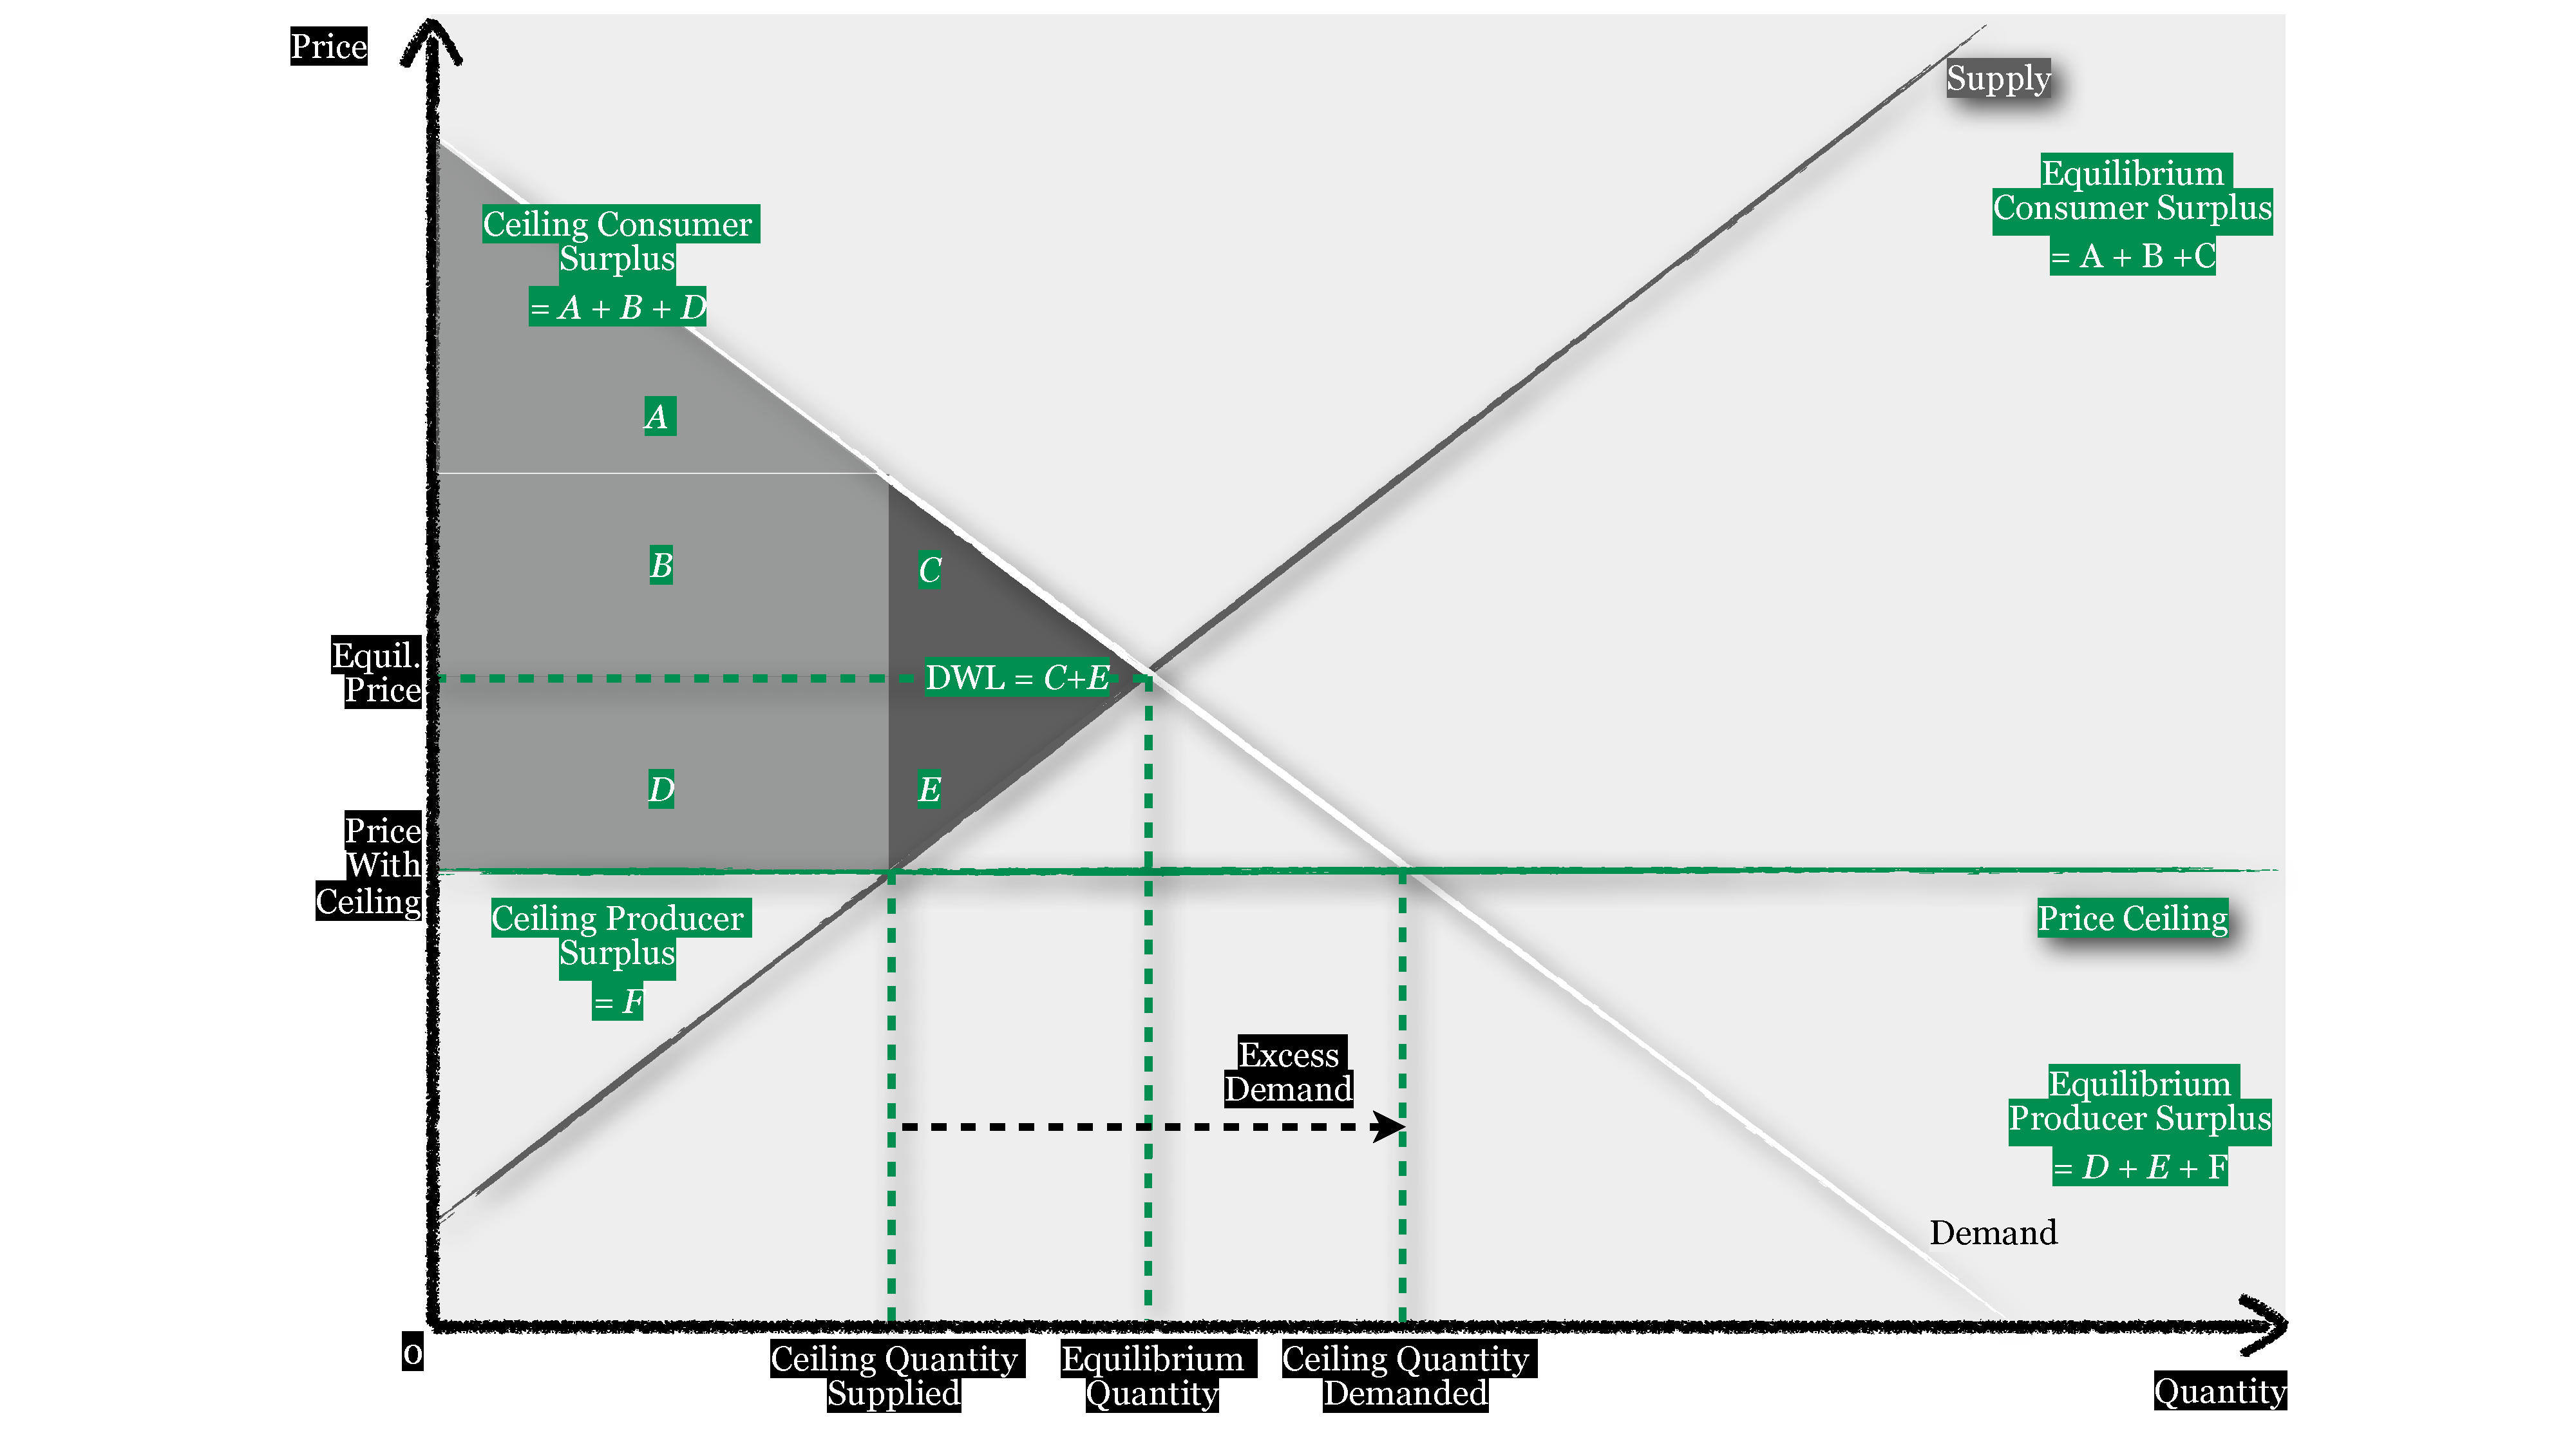
\includegraphics[width=1\textwidth]{price-ceiling}
	\caption[Efficiency and Equity of a Price Ceiling]{The \gls{DWL} and distributive effects of a price ceiling with unit-elastic demand and supply (for example, of housing)}
	\end{center}
	\scriptsize{Compare with \nameref{fig:supply-demand} in \autoref{fig:supply-demand} (p.~\pageref{fig:supply-demand}).}
	\label{fig:price-ceiling}
\end{figure}

\begin{figure}[htbp]
	\begin{center}
	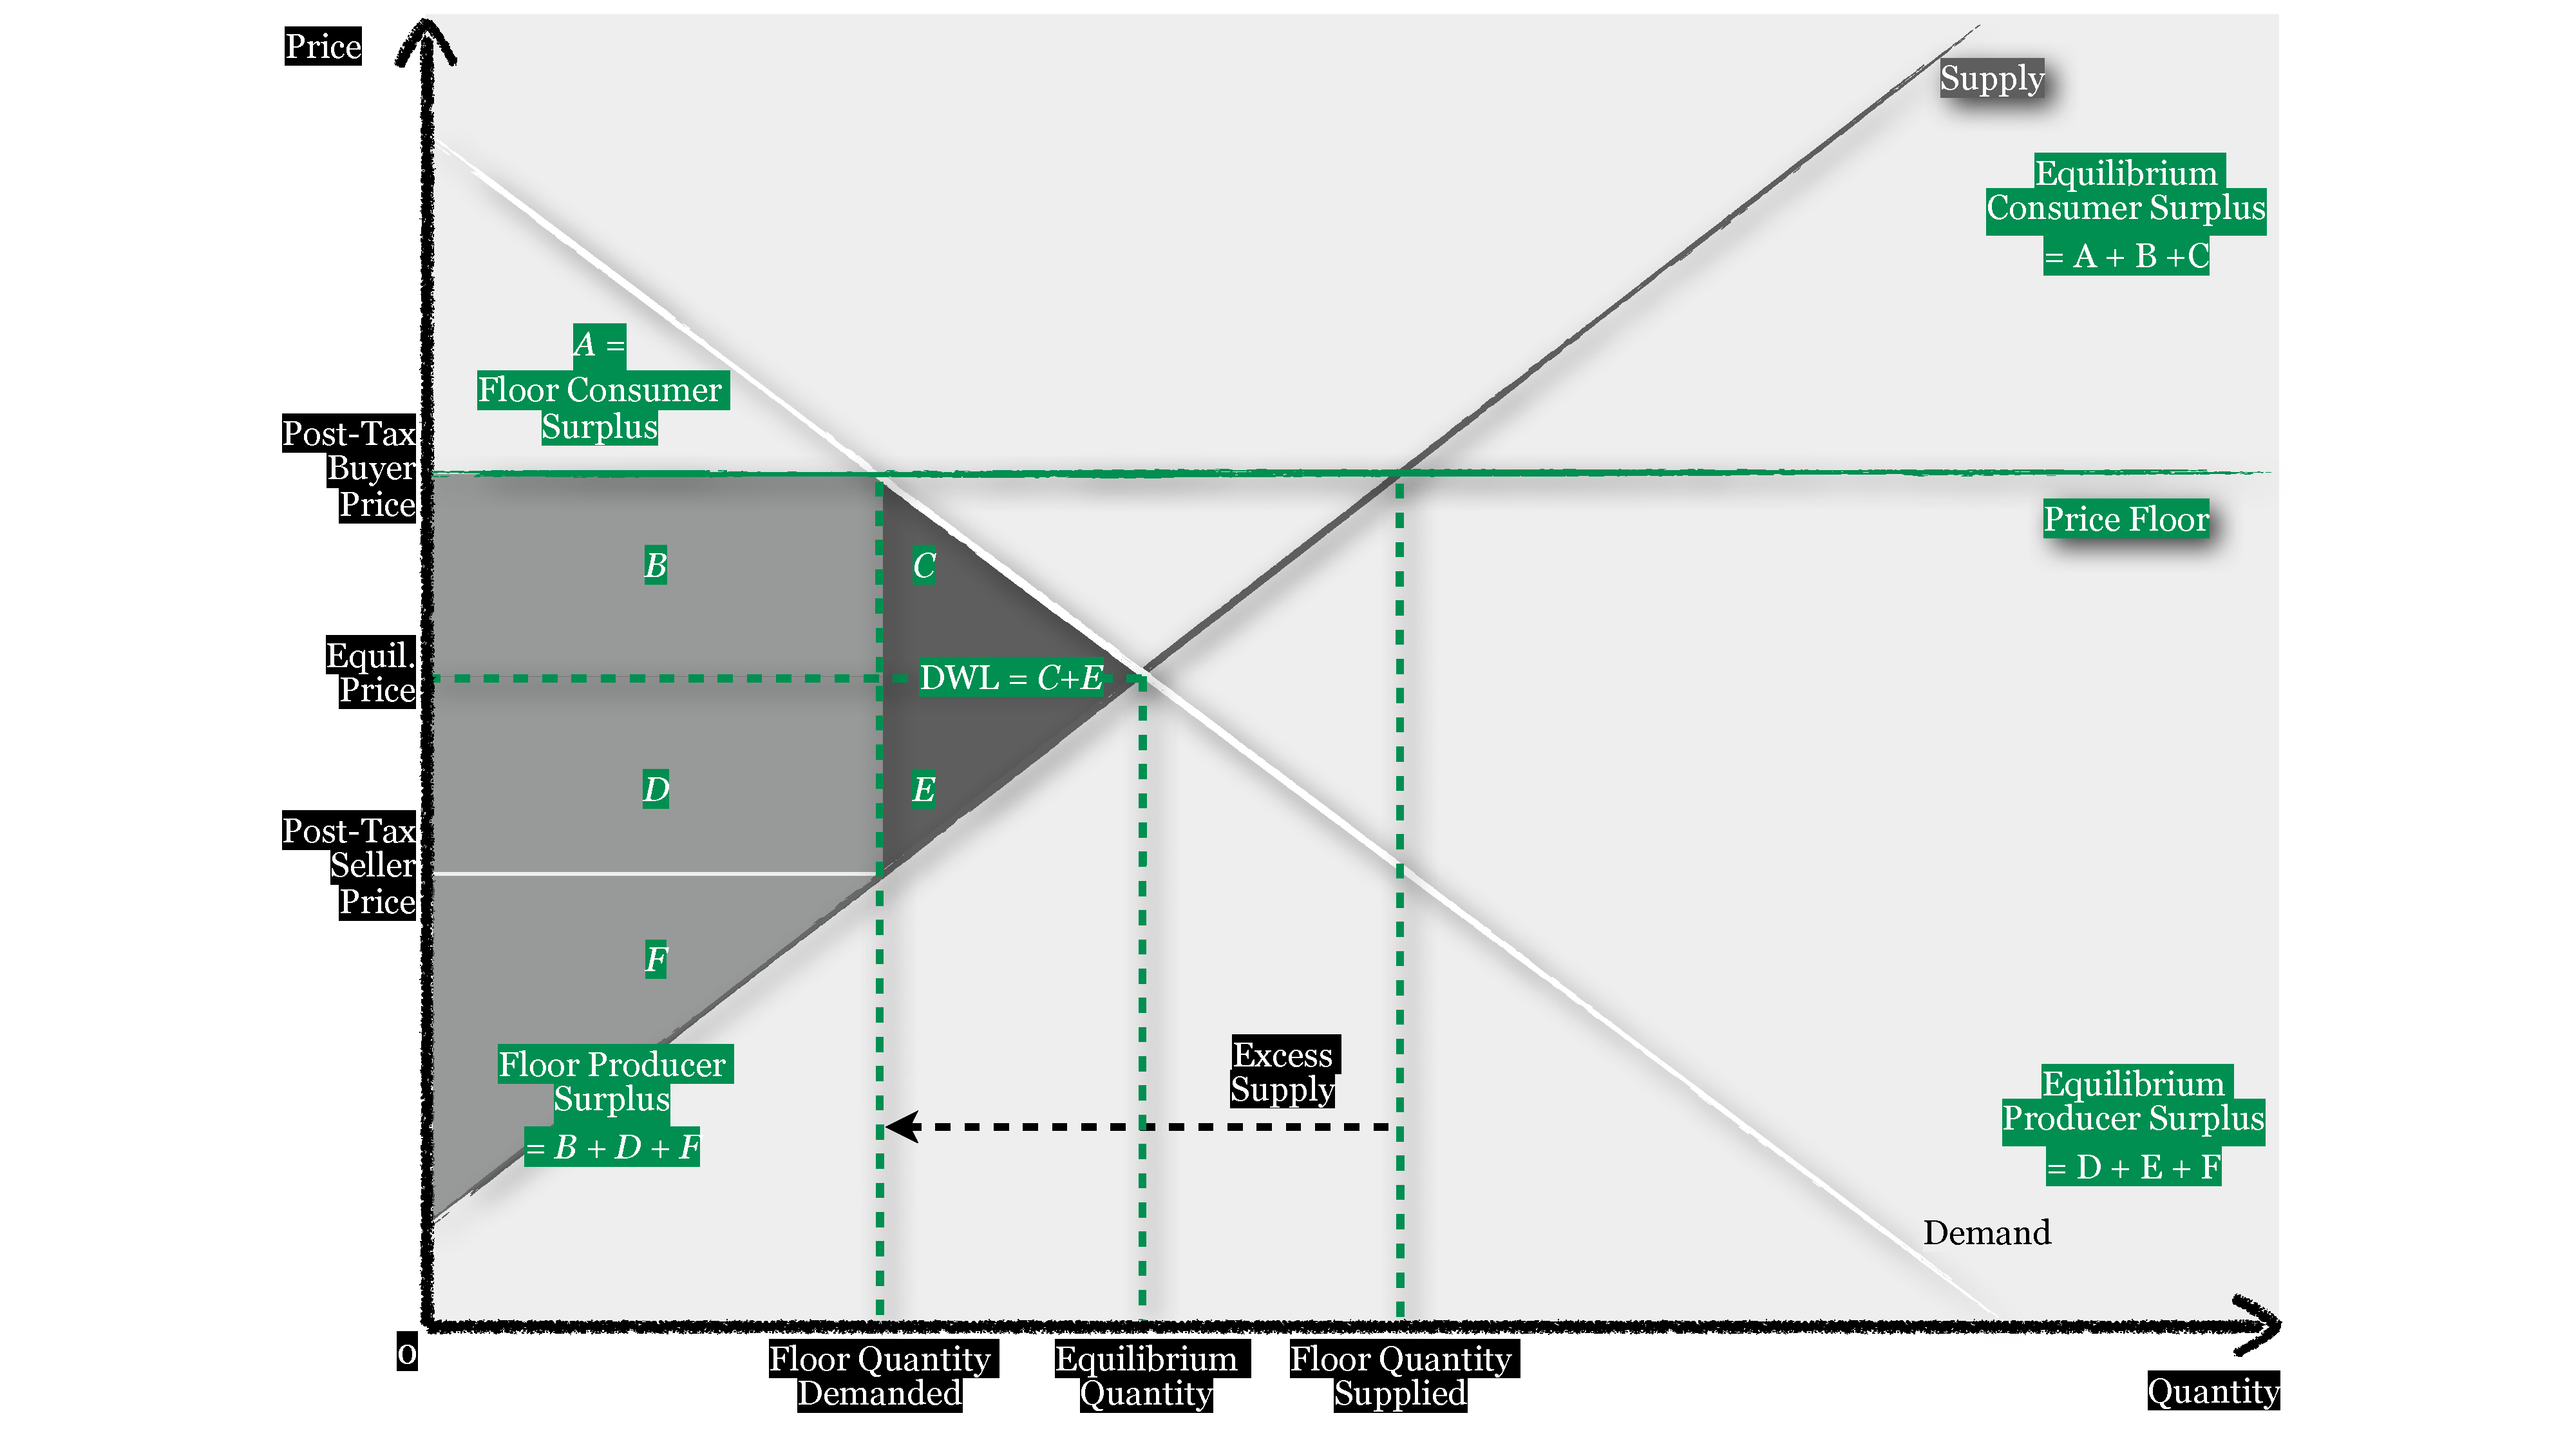
\includegraphics[width=1\textwidth]{price-floor}
	\caption[Efficiency and Equity of a Price Floor]{The \gls{DWL} and distributive effects of a price floor with unit-elastic demand and supply (for example, of labor)}
	\end{center}
	\scriptsize{Compare with \nameref{fig:supply-demand} in \autoref{fig:supply-demand} (p.~\pageref{fig:supply-demand}).}
	\label{fig:price-floor}
\end{figure}

\begin{description}
	\item[Efficiency.]
	In addition to the desired, redistributive zero-sum component, price controls also destroy welfare:
	much like taxes (\autoref{fig:DWL}), they cause a \gls{DWL}.
	Price controls are a negative-sum allocation.
	Ceilings push prices (say, rents) below equilibrium levels, decrease supply (of flats) and increase demand (for flats), causing excess demand.
	Some potential tenants cannot find good housing, even though they would be willing to pay a higher rent or some potential landlords will not built or improve housing, even though willing tenants could be found.
	Conversely, floors push prices (say, wages) above equilibrium levels and increase supply (of labor) and decreases demand (for labor), causing excess supply (unemployment).
	Some workers cannot find gainful employment, even though they would be willing to work for lower pay or some potential employer will not hire an available worker, because her cost (wage) outweighs her utility (productivity).
	Under binding price ceilings or floors, some otherwise pareto-improving exchanges will not be undertaken, causing decrepit real estate
	\footnote{
		Rent control is famously derided as ``the next best way to destroy a city'' aside from carpet bombing.
		%find quote
	}
	or unemployment, respectively.

	Such \glspl{DWL} are the opposite of gains from trade, they invariably reduce to total consumer (producer) surplus of people able to buy (sell) goods at prices lower (higher) than their reservation price.

	The size of the \gls{DWL} of price controls depends on the relative price elasticities of supply and demand (just like the \hyperref[sec:minimal-DWL]{\gls{DWL} of taxes}, p.~\pageref{sec:minimal-DWL}).
	The more price inelastic demand, the smaller is the \gls{DWL} of price floors:
	even at pushed-up prices, few buyers will be able to exit the market and almost all sellers will find buyers.
	Conversely, the more price inelastic supply, the smaller is the \gls{DWL} or price ceilings:
	even at pushed-down prices, few sellers will be able to forego sales and almost all buyers will find sellers.

	In the real world, \hyperref[sec:well-determined-incidence]{elasticity is hard to determine} and depends on many factors (p.~\pageref{sec:well-determined-incidence}).

	In housing markets, supply (landlords) may be inelastic in the short run (for existing housing), but very elastic in the long run (for improved, or new housing).
	\glspl{DWL} (or decrepit housing) are probably sizeable.
	In labor markets, too, demand (employers) will likely not be price inelastic across the board.
	Often, labor can be substituted by capital.
	Here, too, \glspl{DWL} (or unemployment) will be sizeable.
	In any case, it will be very hard for states to gauge elasticities and calibrate price controls accordingly to specific industries, time periods and regions.
	\footnote{
		In addition to the mere complexity of such regulatory intervention, price controls are also prone to rent-seeking clients.
		As the gains (and losses) will often be obvious to, and concentrated in some citizens, they may lobby their government to affect changes \citep{Peltzman1976,Posner1975,Krueger1974}.
		As in oil-rich rentier states \citep{Beblawi1990}, widespread zero-sum games may corrupt politics.
	}
	\item[Effectiveness.]
	Price controls are also limited in their effectiveness.
They may, in principle --- if at colossal cost and complexity --- redress some of the inequities of \nameref{sec:winner-take-all} markets (p.~\pageref{sec:winne-take-all}), \nameref{sec:different-budget-constraints} (p.~\pageref{sec:different-budget-constraints}) and \nameref{sec:diminishing-marginal-utility} (p.~\pageref{sec:diminishing-marginal-utility}).
Short of a near planned economy, they do little to dampen \nameref{sec:positional-race}s (p.~\pageref{sec:positional-race}):
 consumers can simply buy different (more extravagant) categories of goods, or more of the same to fulfill positional impulses.
They can also hardly reign in on \nameref{sec:monopsony-employers} (p.~\pageref{sec:monopsony-employers}).
By definition, their demand for labor is highly price elastic, given plenty of alternatives.
Worker supply of labor, absent another employer, is almost perfectly price inelastic.
\end{description}

Governments should, however, respond to monopsony employers in labor markets either by anti-trust action or by leveling the playing field.
Regulating a right to strike and the right to form trade unions can put monopoly employees opposite monopsony employers in collective bargaining.
\footnote{
	Such as in Article 9, Section 3 of the German Basic Law.
}
Employment protection and labor contract regulation can also alleviate the power imbalance in labor markets.

\subparagraph{Affirmative Action.} \phantomsection \label{sec:affirmative-action} To a limited extent, governments can also respond to winner-take-all markets with affirmative action or equal opportunity legislation.

\subparagraph{Redistribution by Fiscal Policy} \phantomsection \label{sec:fiscal-redistribution} The principal redistributive tool of government is a progressive tax, by which government collects more from the rich to pay for public expenditures, and/or finances handouts to the poor.
\footnote{
	A cash-flow based, post-paid \gls{PCT} (recently \citealt{McCaffery2002,McCaffery2005}), a \gls{LVT} \citep{George1879}, and, if necessary, a \gls{NIT} to fight structural unemployment or working poverty (first suggested by Milton \citealt{Friedman1962}), and a \gls{WT} on net worth to rein in extreme inequity are \hyperref[chap:better-tax]{good taxes} to respond to these inequities (p.~\pageref{chap:better-tax}).

	Notably, even such sharply progressive taxation, may be unable to mitigate the inequities (and welfare losses) of monopsony employer labor markets.
	Potentially, monopsony employers will counteract progressive schedules by further lowering their wages.
	Some regulatory interventions, especially a right to strike and to unionize, may be essential.
}
%this seems to be a very, very short section.
%Maybe expand or refer to other section?

%As the cooperation problem of a Prisoner's Dilemma is hard to resolve\footnote{The non-coercive solution of reciprocity under the shadow of the future \citep{Oye-1985-aa} will not work here:
%it requires infinite or unknown iterations, but life is finite and the distribution of mortality risks (a.k.a.
%life tables) is known.} without coercive (state) intervention, it follows that:
	%add:
%the price of cooperation
	%add:
%winning strategy from computer simulation tit for tat fails bc of initial condition

%\begin{desideratum}[Positional Consumption]
%	A desirable tax discourages excessive consumption of positional, Veblen goods.
%	\label{des:positional-consumption}
%\end{desideratum}


\subparagraph{Redistribution by Monetary Policy} \phantomsection \label{sec:distributive-effects-of-inflation}.
 Monetary policy cannot effectively mitigate inequitable market outcomes.
Inflation and deflation redistribute wealth, but not between the rich and the poor.
Instead, inflation redistributes wealth between credits denominated in real terms (for example, house ownership), debts denominated in nominal terms (for example, a fixed-rate mortgage) and credits denominated in nominal terms (for example, fixed-rate pension) and debts denominated in debts denominated in real terms (for example, a futures contract) as summarized in \autoref{fig:distributive-effects-of-inflation}.

\begin{figure}[htbp]
	\centering
	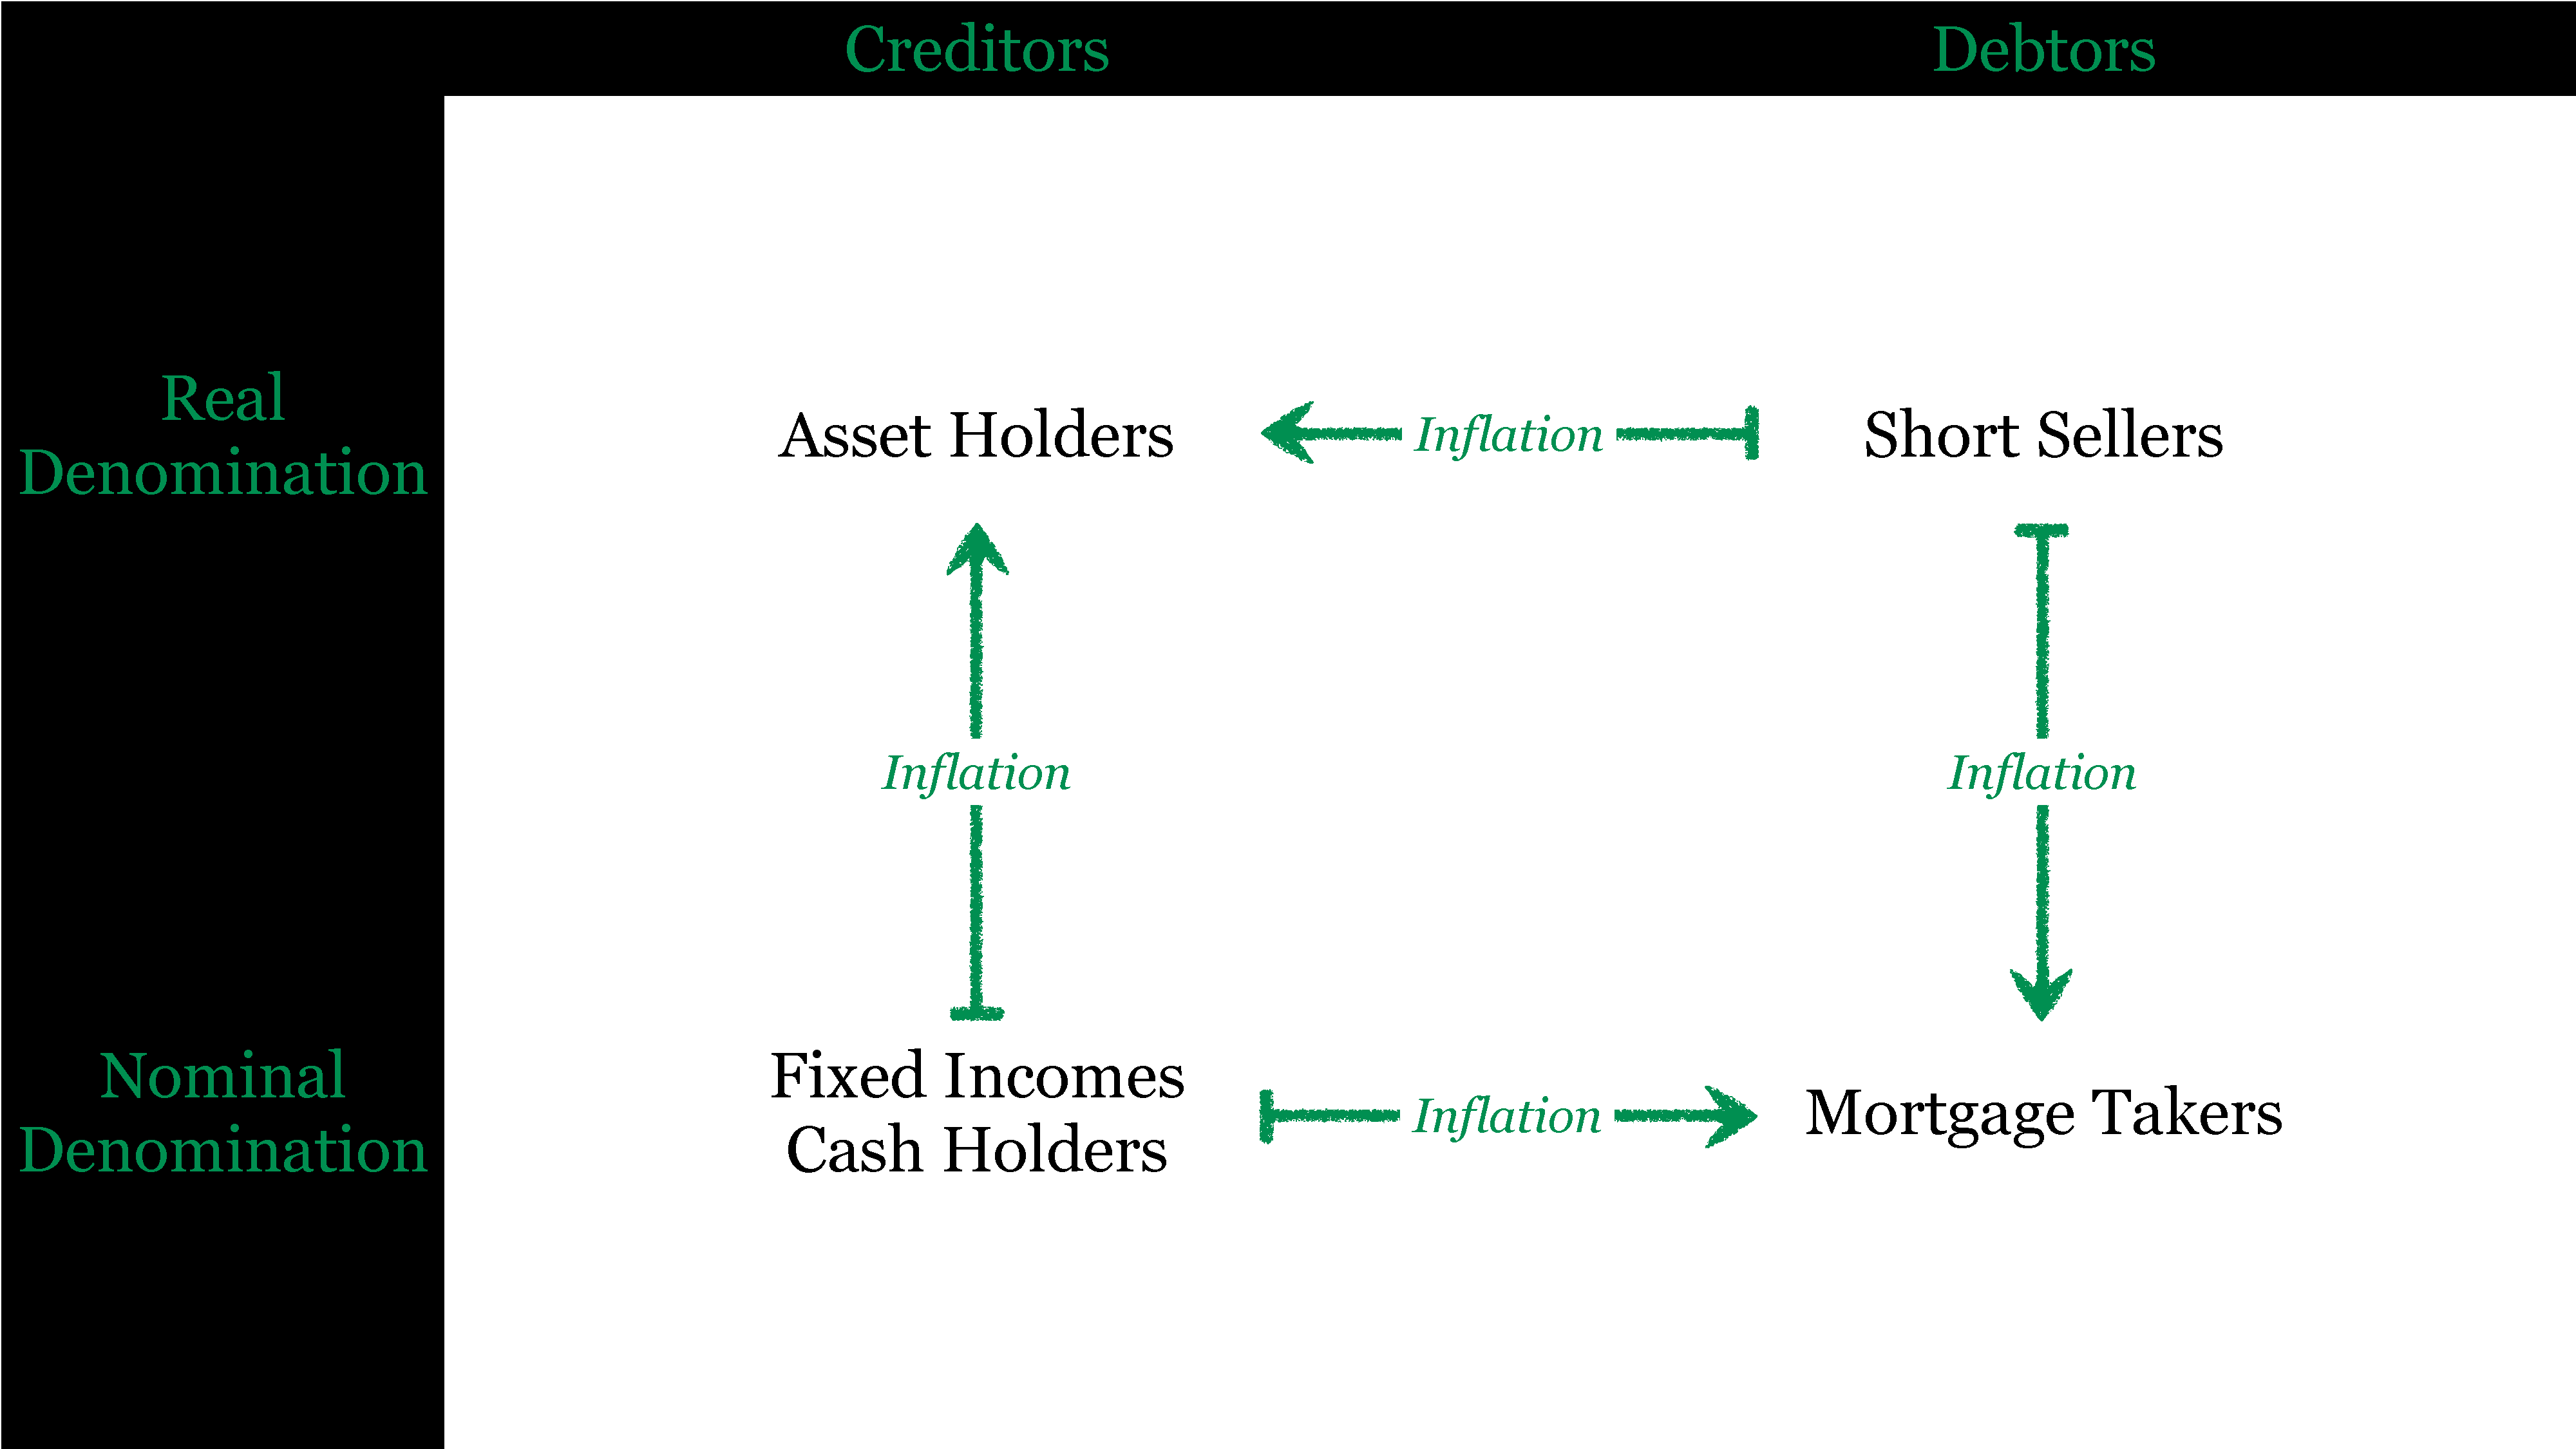
\includegraphics[width=1\textwidth]{distributive-effects-of-inflation}
	\caption[Distributive Effects of Inflation]{The distributive effects of inflation, with some examples}
	\label{fig:distributive-effects-of-inflation}
\end{figure}

Such arbitrary redistribution does not correspond to \nameref{sec:inequality-dynamics} of markets  (p.\pageref{sec:inequality-dynamics}) and cannot be defended on normative grounds.
\footnote{
	Rich people are more likely to be creditors, and poor people more likely to be debtors.
	Telling, as \cite{Coggan2011} does, the history of mankind as the struggle between debtors and creditors \citep[paraphrasing][]{Marx-1867-aa} may be roughly adequate and enlightening, but the simplification carries only so far.
	As \cite[K6-24-04]{Coggan2011} himself points out, German hyperinflation wiped out the (often nominally denominated) savings of the middle class, but left relatively unaffected the (often real denominated) wealth of the upper class and the subsisting lower class with neither debt nor savings.
}

Additionally, redistributing by monetary policy causes severe \hyperref[sec:price-stability]{welfare losses} (p.~\pageref{sec:price-stability}.
Today, as financial products have diversified, redistributing based on denomination and between creditors and debtors will have increasingly arbitrary results.
\footnote{
	There is a case to be made for deliberately sharing the burden of systemic and unsustainably high levels of debt, as may be case with Greek sovereign debt in the 2007ff financial crisis \citep{Coggan2011}.
	As \citeauthor{Coggan2011} reminds us, we do not need inflation to achieve that;
	a (partial) default will do the trick, colloquially referred to as a ``haircut'' in the 2007ff financial crisis.
}

Monetary policy on distributive goals, as on \nameref{sec:production} (p.\pageref{sec:production}), shines by staying neutral.
It must strive to maintain price stability to avoid any arbitrary and undue distributive effects that would otherwise interfere with the distributive dynamics of state and market.

\subsection[Consistency Over Time]{Consistency Over Time:~Saving Tomorrow's Pie}\label{sec:time}

\paragraph{The Human Condition in Time}
Human beings are myopic planners \citep{KahnemanTversky1979}.
They discount the future hyberbolically;
the more remote a future event is, the more humans discount its rewards (\citealt{Ainslie1975}, \citealt{Thaler1981}).
Human beings also succumb to herding:
they do as others around them do.
%citation needed.
Both these frailties can lead to time inconsistency, where we simultaneously hold incompatible preferences for our present and future selves, for example when we would like to retire somewhere warm and mild, but also want a new car every three years.

To be time consistent, we have to do unto future generations (or selves) as we would have them do unto us (the Golden Rule of reciprocity).
Applied to the material world, we have to save --- at least --- at that level, which allows the highest constant level of current and future consumption (\citealt{Phelps1966a}, \citealt{Solow1956}).
If we are more generous to our children, or consider technological innovation to be endogenous, we might have to save even more.

Time consistency bears both on equity and efficiency.
An \emph{equitable} policy ensures same (discounted)
\footnote{
	\label{fn:3components}
	In his treatise on the economic costs of global warming, \citeauthor{Stern-2006-aa} lists three components to discount to future utility:
	\begin{inparaenum}[\itshape 1\upshape)]
		\item future people may value an additional unit of consumption less (or more) if they have more (or less) output available overall (elasticity of marginal utility).
		\item expected but \emph{exogenous} growth, such as a chance discovery of a new technology, may increase future output without requiring present people to give up anything.
		\item people will discount future utility simply because it is in the future and uncertain (the pure discount rate of the future) \citep[52]{Stern-2006-aa}.
	\end{inparaenum}
}
utility for people living today vs.\ people living in the future.
An \emph{efficient} policy ensures maximum (discounted) growth over all periods (along the long-term growth path of the economy).
%needs citation, adequate terminology.

\paragraph{Interest} \phantomsection \label{sec:interest} In the exchange economy, capital markets align preferences of present and future generations (and selves) by compensating savers with an interest.
Ideally, risk-free interest rates,
\footnote{
	Idiosyncratic risk of specific investments are diversified or hedged away.
	Risk-free interest rates still include a premium for \emph{systematic} (not systemic) or aggregate risk, such as the continued existence of life on earth.
	The remaining interest component, the pure discounting of future utility, represents the hedonic loss of present, myopic individuals.
}
and other (hedged) returns on capital (for example, stock market indices) equilibrate at that level, where future marginal utility equals present marginal cost of saving.
At this intertemporal optimum,
\footnote{
	Specifically, saving (below \citeauthor{Solow1956}'s optimal rate) without interest is a \citeauthor{Kaldor1939}-\citeauthor{Hicks1939} improvement:
	future utility is greater than present cost.
	Interest can be considered an intertemporal sidepayment from the future to the present.
	With interest, sub-optimal level saving can be pareto improved:
	upon saving more, both present and future generations (and selves) are at least equally well off.
}
we follow the Golden Rule:
present generations (and selves) \emph{do} unto future generations (and selves) as vice versa.

Under the assumptions of neoclassical orthodoxy, efficient capital markets should guarantee \emph{some} degree of time consistency.

\subparagraph{Garbage In, Garbage Out.} But because markets are ultimately \emph{aimless} and operate on (assumed!) \emph{exogenous} preferences, the \emph{formal} ability of capital markets for intertemporal optimization is strictly limited.
Interest rates --- as all other prices --- are elegantly aggregated (time) preferences of people.
If these preferences are inconsistent, or amoral, so, too, will be the resulting market ``optimum''.
As in statistical analyses, no matter the algorithm, the quality of the output depends strictly on the quality of the inputs.

People may be relatively consistent --- or at least our best bet --- to gauge some components of observed discount rates, including the likelihood of exogenous growth (innovation), or continued human existence (compare footnote \ref{fn:3components} (p.~\pageref{fn:3components}).
For these components, people may input reasonably good `data', and markets will output reasonably good prices.

By contrast, the `data quality' of \emph{pure discount component rate of the future} --- discounting future utility simply because it lies in the future --- is deeply questionable for reasons (compare footnote \ref{fn:3components} (p.~\pageref{fn:3components}):

\begin{enumerate}
	\item \emph{Inconsistency.} People are, as cognitive psychology has shown, \emph{time inconsistent} even in their own lives, and the short- to medium term (\citealt{Ainslie1975}, \citealt{Thaler1981}).
	If they are similarly inconsistent  when deciding how much saving to supply at any given interest rate, \emph{overall} interest rates will be distorted.
	Myopic individuals will \emph{cause} the very inflated interest rates meant to keep their short-sightedness in check, and overall saving will be too low.
	\footnote{
		Myopia implies a \emph{shift} in the supply curve of saving.
		For any given interest rate, people will supply less.
	}
	\item \emph{Morality.} As \cite[54]{Samuelson2005} has recently reminded us, \emph{term uncertainty}, especially pure discounting of the future is a \emph{normative concern}.
Just how much we value the welfare of future generations and selves is a \emph{moral} judgement.
There is nothing in our nature or our environment that could positively tell us what a \emph{true} rate would be, there are only normative judgments of what a \emph{right} rate should be.
Once people have agreed on such a rate, markets can do the \citeauthor{Hayek1931}ian number crunching.
But markets, because they will accept \emph{any} rate as input, cannot solve this moral problem for us.
Instead, only a democratic polity --- and its government --- can decide the pure discount rate.

	People often say they want their children to live a \emph{better} life.
If similar sentiments are deeply-held and widespread, people might democratically decide to save \emph{more} than intertemporal \emph{equity} demands.
If indeed, we shall give to our children \emph{better}, than we ourselves received, we are at least looking for a \emph{Kaldor-Hicks} (not Pareto!) improvement without and above the equilibrium capital return.
\end{enumerate}

Even ignoring such substantive concerns, real world capital markets are also plagued by \emph{formal} intertemporal failures, causing their own costly and inequitable time inconsistency.
The capitalist algorithm not only receives bad inputs, but it is also ridden with bugs, that fail both in the short and the long term.

\paragraph{Short-Term Intertemporal Failures} \label{sec:short-term-inconsistency} Economic activity tends to fluctuate in the short-term.

\subparagraph{Business cycles} are periodic fluctuations, typically relatively mild in amplitude and slope.
They are endogenously caused by lumpy, lagged decision-making of market participants, for example in inventory cycles.
\footnote{
	\emph{Endogenous} business cycle durations range from 3--5 years for lagged inventory decisions \citep{Kitchin1923}, 7--11 for fixed investment \citep{Juglar1862}, 15--25 for infrastructural investment \citep{Kuznets1930} and 45-60 for technological revolutions \citep{Kondratiev1925}.

	For a recent empirical test of all four business cycle theories, see \cite{Korotayev2010}.

	The latter two of these are probably beyond reliable anticipation and certainly beyond the short-term.
	They are also contested as empirical artifacts \citep{Howrey1968} or restricted to heterodox, evolutionary economics \citep{Modelski2010}.
}

According to the dissenting, minority view, business cycles are \emph{true} shocks that may or may not be endogenously amplified, but are exogenous in origin (\citealt{Kydland1982}).
\footnote{
	\gls{RBCT} proponents consequently argue against state interventions to counteract these exogenous shocks.
}

\subparagraph{Bubbles and panics} can lead to abrupt and dramatic fluctuations in economic activity, with great slope and amplitude.
Bubbles and panics envelope market actors when they make their decisions based on the anticipated decisions of others, in a beauty-contest type game \citep{Keynes1936}.
Similar rationales also emerge when making privately informed decisions creates a positive externality for other participants to free-ride on your inadvertently disclosed information \citep{Banerjee-1992-aa}.
\footnote{
	For a fully-fledged account, involving the debt, equity and asset market as well as monetary and regulatory correlates of \emph{Maniacs, Panics and Crashes}, see \cite{KindlebergerAliber-2005-aa}.
	Herding has also been complemented and expanded into the (heterodox) debt-deflation theory of economic cycles, where credit cycles magnify initial bubbles, panics or shocks \citep{Fisher1933}.
}

\subparagraph{Fluctuations are Costly.} Both types of fluctuations in economic activity are inefficient because they temporarily leave factors of production idle (overused) and increase periodic transaction costs.
Fluctuations leave factors of production (for example, an assembly line) idle during the downturn or building up excess capacities during the upturn (for example, a real estate overhang).
Additionally, fluctuations cause unnecessary adjustment costs (for example, storing equipment).
The costs of short-term fluctuations are particularly virulent in labor markets, where hiring is expensive and unemployment can degrade worker morale.
Aside from these material costs, short-term and uncertain employment (and economic prospects in general) cause stress and hardship.
%this needs a source

Such idleness or mania diverts the economy away from its (exogenously) long-term growth path and thereby slows down the economies progress along the growth path.

By contrast, ``true'' exogenous shocks (such as an earthquake) or genuinely new information about future utility of present savings (for example, because of a new technology) is not a deviation from, but a \emph{shift} of the long-term growth path.
It is, for better or for worse, unavoidable.

\paragraph{Short-term:~State responses}
States can respond by regulatory, fiscal and monetary means to reduce the frequency, depth and duration of economic fluctuations.
In the following, I discuss the state responses to a downward deviation from the long-term growth path of the economy.
States should likewise, if with opposite sign, respond to upward deviations from long-term growth.

\subparagraph{Regulatory}
States can reign in on short-term downturns simply by outlawing respective actions of market participants.
\gls{EPL}, for example, can include lay-off protection, making it harder for employers to fire workers in a downturn.
Other regulatory interventions include the bans on short-selling of recent 2007ff fame.
%maybe discuss decommodification again, here.
%Why does this, or does this not, belong in here?
%I think decommodification is a second-order consideration, that's why it doesn't belong in here.

Regulatory responses can be effective, but blunt instruments as they also affect economic activity outside of endogenous downturns.
Generous lay-off protection, for instance, can cause a \gls{DWL} of unemployment during upturns, keeping the economy under its long-term growth path.
Regulatory interventions can also fail to distinguish between endogenous and exogenous fluctuations in the economy overall and some of its markets.
\footnote{
	Generous lay-off protection has been hypothesized to contribute to ``eurosclerosis''.
	%citation, explanation needed
}
As collateral damage, generous lay-off protection may prevent workers from moving to new, more productive firms and sectors (for example services rather than mining).
Similarly, bans on short-selling may prevent or defer necessary market readjustment in case of real, exogenous price shocks (for example, a war in an oil-exporting country).

\subparagraph{Fiscal Stimulus.} \phantomsection \label{sec:fiscal-stimulus}
States can also respond to short-term downturns by propping up aggregate demand, following \citeauthor{Keynes1936}ian demand management.
\footnote{
	According to the opposing, now minority view of \gls{RET}, fiscal expansion will be ineffective, because market participants will correctly anticipate that current deficit spending (expansion) will be offset by future tax hikes (contraction).
	Anticipating such future losses, they will hoard more cash and equivalents today, than they would otherwise, thereby negating any current period effect.

	Even though controlled experiments are not readily available at the level of entire economies, deficit spending seems to work, at least a little.
	Here, for once, human ignorance (of \gls{RET}) is not only bliss, but also a blessing for all of us.
}

By definition, to push up aggregate demand, government must \emph{dissave}.
Fiscal stimulus must be paid out of newly issued debt, or prior savings --- but it cannot be paid out of increased \emph{current} period tax revenues, for such hikes would cut private demand, as public demand expands.
\footnote{
	A democratic polity can \hyperref[sec:trade-offs]{trade off} public for private demand as it wishes (p.~\pageref{sec:trade-offs}), but any such balance will not affect aggregate (public \emph{and} private) demand.
	Democracies can call this shot, but it will not alleviate slumps.
}
Still, even \emph{deficit spending} will \emph{crowd out} some private demand, as it soaks up savings in capital markets.
Government bonds must be sold to someone, and that someone will not be able to spend or invest that same money elsewhere.

Luckily for government (and all of us), it can target its spending wisely to those areas where it will have a maximum \emph{multiplier effect}, that is, where demand begets as much more demand as possible.
For example, when government procures a new railroad line, these construction workers will have more resources to spend on entertainment, or invest in a family home.

Of course, government demand is not the only demand that multiplies;
private demand also multiplies.
However, because government (ideally) aims \emph{not} to maximize profit, but overall economic recovery, it can seek out that spending that maximizes multiplication.
Private demand, by contrast, will seek maximum profit at low risk, which, in economic downturns, is often found in a ``flight to safety'', hoarding of cash or equivalents.

A good stabilizer should go entirely into immediate consumption or investment, and possibly incentivize further dissaving.
\footnote{
	The 2009 German \emph{cash-for-clunkers} scheme --- for all its infamous waste, cannibalizing effects and blatant clientelism --- included such an incentive:
	car buyers had to top-up the subsidy with own savings to buy a new car.
}

While easier to understand for the often maligned deficit spending type of stimulus, governments must trade off the multiplication effect versus the crowding out effect during \emph{all} fiscal expansions.
Even when (or rather, hypothetically, \emph{if}) governments were to pay for stimulus ``out of pocket'', these now dispersed savings were collected at an earlier time, ever since they crowded out that same amount in private demand.

Maximizing multiplied demand, for every increment of demand crowded out is a challenge that government must always face in fiscal expansion.
Where to best direct resources is an empirical question for econometricians, statistical physicists and other experts that I happily need not, and cannot engage here.


\emph{Automatic stabilizers} can support demand without legislative intervention.
They include unemployment insurance
\footnote{
	To the extent that it serves as an automatic stabilizer and/or pools the near-universal risk of unemployment, ``unemployment insurance'' is, again, a misnomer.
	The demand stabilization bought by unemployment benefits are a public good, idiosyncratically financed out of a specific tax in many countries.
	%add respective footnote, i talk about this somewhere else.
	%This isn't quite right yet.
	%Check desideratum from MPP RedistributionAndRevenueAreOne
}
and short-time working benefits, both of which smooth out (consumer) demand by substituting the market income of laid-off, or shorted workers.
\footnote{
	(German) automatic stabilizers have recently faired well during the 2007ff financial crisis and received great praise by \glspl{IFI} (\citealt[20]{IMF-2008-ab}, \citealt[19]{WorldBank2008}) and experts \citep[8]{BofingerFranz-2007-aa}.
}

\emph{Discretionary stabilizers} are often called for when bubbles, panics or amplified shocks cause output fluctuations too large and fast to be captured by automatic stabilizers.
They come in the form of tax breaks, stimulus subsidies or public investment.
They, too, rely on dissaving, and the incurred debt must be repaid in good times.

\emph{Side effects.} As all potent drugs, fiscal stimulus must be prescribed with great care.
It has at least two dangerous side effects:
\begin{enumerate}
	\item \emph{Structural painkiller.} All stabilizers can disguise real needs for adjustment as cyclical problems, further diverting an economy from its equilibrium and long-term growth path.
	\item \emph{Playing favors.} Especially discretionary stabilizers are also prone to clientelism, that easily creeps in when legislatures pass often very targeted stimulus packages.
When specific decisions are made, rather than general rules passed \citep{Weber-1918-aa}, as discretionary stabilizers require, special interests are more likely to gain the upper hand.
	\footnote{
		The 2009 \gls{VAT} break handed out to the hospitality sector by the new liberal-conservative coalition in Germany is a recent, brazen example.
	}
\end{enumerate}

\subparagraph{Monetary Stimulus.} \phantomsection \label{sec:monetary-stimulus}
Government can also prop up the economy in the short run by monetary stimulus.
\footnote{
	Technically, central banks can lower the (federal funds) interest rate by buying (back) government bonds (\emph{\gls{OMO}}), pump cash in the economy by buying assets (\glsfirst{QE}) or accept riskier collateral from commercial banks (\emph{qualitative easing} \citep{Buiter2008}).}.
	Government injects more cash into the economy, to make up for liquidity frozen up during the downturn, thereby \hyperref[sec:price-stability]{holding the money supply \emph{constant}} (p.~\pageref{sec:price-stability})\footnote{
	``Monetary expansion'' is thereby a misnomer.
}

The monetary contraction in the course of an endogenous downturn can best be described as a general loss of confidence in the profitability of future projects (such as investments).
As market participants become squeamish about economic prospects in general, they hoard cash (or equivalents) or flee to safety (such as gold, or --- before 2009 --- government bonds).
\footnote{
	This is the (Post-)Keynesian consensus.
	%source
	Strict monetarists argue that the money supply \emph{always} remains at equilibrium without government intervention.
}
Less funding is available even for the most profitable and unrisky projects and the lack of liquidity can render (balance sheet) solvent firms (cash flow) insolvent.
The money supply contracts.
When these defaults further feed the market panic and cause more debts to sour, a self-reinforcing debt-deflation crises may ensue.
%add citation

A monetary stimulus bolsters market confidence by essentially placing an optimistic, massively government-backed bet.
When central banks resort to quantitative or qualitative easing, they declare whichever assets they buy or collateral they accept as worthwhile (profitable) investments by fiat.
When, if and to the extent that markets buy into this stunt of optimism, they will be increasingly willing to lend the injected (and their own) money again, too.

Monetary stimulus has some drawbacks, too.
Monitoring the money supply in the economy is very difficult and imprecise, and related policy imperatives are incompletely understood.
To avoid inflation, central banks must contract their money supply again as soon as the monetary stimulus has worked, and market liquidity has recovered.
The timing and calibration of interventions to maintain a constant money supply are crucial, but difficult to get right.

Monetary stimulus, too, can disguise and defer unavoidable realignment when the cause of the downturn is exogenous, such as a true price shock (as for example when revised Greek fiscal numbers became available in 2008).
When the long-term growth path is shifted (downward), the money supply \emph{must} contract in absolute terms as the underlying economy, too, will contract, or at least grow slower than previously expected.
Monetary stimulus does not allow economies to live beyond their real, exogenous means for long;
it just defers the pain to a later contraction or risks inflation, which in turn \hyperref[sec:distributive-effects-of-inflation]{.
distributes the costs of realignment arbitrarily} (p.~\pageref{sec:distributive-effects-of-inflation}.

%this needs to be further tied in with the general section explaining money.
	% not sure where such a section would be, do I really need it?
	%It really doesn’t much matter which kind of inflation targeting you’re using here.
	%Actually think again about that.
%You mind need constant money supply.

\paragraph{Long-Term Inconsistency} \label{sec:long-term-inconsistency}

\subparagraph{Market problems} The market institution of equilibrium interest rates may fail to guide humans to temporal consistency in the long run for three reasons.

\begin{enumerate}%I think I need to introduce Solow before this \ldots
	\item (Exogenous) growth theory discussed so far assumes technology to be constant, or exogenous:
as if the rate at which new technology is discovered cannot be altered by humans.
Accordingly, once a maximum steady-state output is achieved, further \emph{capital deepening} or other policy will be inconsequential for growth.
Exogenous technological innovation appears unreasonable in a knowledge-based economy (as recently endorsed in \citealt{Communities2009}).
When we \emph{can} endogenously improve our creativity, we might have to save more to achieve intertemporal Kaldor-Hicks improvements.

	Additionally, markets may fail to adequately save for and invest in fundamental \gls{RnD}, because innovation is often a \hyperref[sec:public-good]{public good} (p.~\pageref{sec:public-good}).
Market innovation may also be hampered by \hyperref[sec:principal-agent-problem]{principal-agent problems} under asymmetric information (p.~\pageref{sec:principal-agent-problem}).

	\item Ancillary conditions frequently observed in post-industrial economies imply \emph{real} (public or private) \hyperref[sec:delta-net-worth]{dissaving} and require offsetting, greater \emph{nominal} savings (p.~\pageref{sec:delta-net-worth}).
	They include aging,
	\footnote{
		The second demographic transition delivered low, often below-replacement level \gls{TFR} and low mortality (\citealt{Davis1945}, restated by \citealt{Caldwell-1976-aa}).

		US 2009 estimated \gls{TFR}:~2.05 \citep{CIA2009}, Germany 2009 estimated \gls{TFR}:~1.41 \citep{CIA2009}, EU-25 2002 \gls{TFR}:~1.37 \citep[2]{Demeny-2003-aa}.
		Life expectancy at birth for EU-25 is 69 years for males and 78 years for females \citep[2]{Demeny-2003-aa}
	}
	structural unemployment,
	\footnote{
		When understood endogenously, strata of underqualified workers are also a real (if not nominal) dissaving in human capital.
		Saving, then, means to (publicly) educate most everyone to be competitively productive in a skill-based economy that outsources or offshores much of manual labor.
	}
	or, equivalently, \hyperref[itm:non-linear-returns]{Baumol's Cost Disease} (p.~\pageref{itm:non-linear-returns}), underprovided public goods (basic research?) and overused common goods (\citealt{Stern-2006-aa}:
climate change!).
Markets can, by definition, not provide these goods or solve these problems, and to the extent that government (or lovers) have neglected to do so in the past, these failures constitutes real dissavings.

	\item Market return rates on capital set a saving rate by equilibrating \emph{self-interest}.
Savings rates, however, are a public good, which cannot be provided out of self-interested exchange.
One person's saving  bestows a positive externality on other people in two ways:

	\begin{enumerate}
		\item When technological change is held to be \emph{exogenous}, other people will benefit from capital deepening and approximating of steady-state growth.
		\item When technological change is allowed to be endogenous, these benefits include greater economy-wide productivity and innovation and will be even larger.
	\end{enumerate}

	Markets, when left to their own devices, will save less than optimal because not all of the societal benefit can be recouped in interest payments.
%add citation from the tax book here.
\end{enumerate}

\subparagraph{Government Saving.} \phantomsection \label{sec:government-saves} If the polity has democratically prescribed a savings rate and/or the market fails to save at positively optimal levels, government can prop up saving by regulatory and fiscal means.

In \emph{regulatory} policy, government can mandate citizens to save into a pension or other saving scheme.
\footnote{
	It does not matter for the economy-wide savings rate whether citizens save into privately offered financial products or state-guaranteed (often \gls{PAYG}) schemes.
	I discuss the (somewhat epiphenomenal and misconstrued) \hyperref[sec:pensions]{difference between private and public pensions} later (p.~\pageref{sec:pensions}).
}
Mandatory pensions and similar financial products solve time inconsistency both at the individual level (present and future self) and the societal level (present and future generations).

The difference between fiscal and regulatory policy I draw in \autoref{tab:ends-mixed-economy} (p.~\pageref{tab:ends-mixed-economy} is a bit murky and overdrawn, when it comes to saving.
 Here is my attempt to draw it anyway:
\begin{description}
	\item[Regulatory] I treat policy as regulatory, when it ties made contributions to \emph{entitled benefits} later in life.
	Much like when it is fencing the commons, government guarantees legally enforceable, quasi-property in both private and public pension schemes.

	Such a regulatory pension scheme, tying benefits to contributions, organises intertemporal production (saving) and distribution (dissaving) in a \emph{single} institution --- much like the market economy does.
	\footnote{
		Real existing (public) pension schemes are a lot murkier and less \hyperref[sec:ordoliberal-hygiene]{ordoliberally hygienic} (p.~\pageref{sec:ordoliberal-hygiene}.
		Frequently, pension schedules feature equity or other policy goals such as child-rearing.
		In these, more realistic cases, the link between contributions and benefits is distorted.
	}
	\item[Fiscal] I treat a policy as fiscal, when contributions do \emph{not} entitle payers to specific benefits.
	By definition, this is what taxes do.

	In fiscal policy, government can encourage private saving with clever subsidies or save resources itself by raising more taxes than spending in the current period.
Government can invest budget surpluses in publicly run projects such as education or infrastructure, or privately run enterprises in \glspl{SWF} (here again, the public-private \hyperref[sec:trade-offs]{trade-off} is irrelevant to the saving component (p.~\pageref{trade-offs}).

	Such a fiscal intertemporal regime keeps intertemporal production (saving) and distribution (dissaving) apart.
Each step in the intertemporal deal requires a separate political decision.
For example, government will have to decide when to auction off \glspl{SWF} and what to use the revenue for.
\end{description}

%\subsection[The Short Term]{In the Short-term:
%Consumption Smoothing.} \phantomsection \label{sec:ShortTermSmoothing}
% \emph{Short-term} fluctuations in economic output are predominantly described as either entirely endogenous\footnote{The usage of ``endogenous'' and ``exogenous'' here does not entirely overlap with their (varied) usage in economic debate.} artifacts of lumpy, lagged decision-making, endogenous herding behavior or as systemically amplified, exogenous shocks\footnote{For a dissenting, minority view, consider \cite{Kydland1982}.
%\emph{Real Business Cycle Theory} suggests there are only ``true'' exogenous shocks, minimizes systemic amplification and argues against all discretionary or automatic interventions.}.
%The characteristics of both expansions or booms and contractions or recessions are roughly symmetric.
%For simplicity, I concentrate here on policy imperatives during a cyclical downturn, but recommendations hold equally, if with opposite sign, for upturns.

%\paragraph{Endogenous Cycles.}\phantomsection \label{sec:BusinessCycles} Three \emph{ideal types} \citep{Weber-1920-aa} of endogenous fluctuations can be distinguished.
%They are qualitatively different and call for different policy responses.
%Empirically, however, they may not be distinct.

%\subparagraph{Business Cycles.} Business cycle durations range from 3--5 years for lagged inventory decisions \citep{Kitchin1923}, 7--11 for fixed investment \citep{Juglar1862}, 15--25 for infrastructural investment \citep{Kuznets1930} and 45-60 for technological revolutions \citep{Kondratiev1925}\footnote{For a recent empirical test of all four business cycle theories, see \cite{Korotayev2010}.}.
%The latter two of these are probably beyond reliable anticipation and certainly beyond the short-term\footnote{They are also contested as empirical artifacts \citep{Howrey1968} or restricted to heterodox, evolutionary economics \citep{Modelski2010}.}.

%Amplitudes as well as slopes of these lumpy, lagged decisions both tend to be relatively mild.

%\paragraph{Endogenous Bubbles and Panics}\phantomsection \label{sec:BubblesPanics} envelope market actors when they make their decisions based on the anticipated decisions of others, in a beauty-contest type game \citep{Keynes1936}.
%Similar rationales also emerge when making privately informed decisions creates a positive externality for other participants to free-ride on your inadvertently disclosed information \citep{Banerjee-1992-aa}.
%When ``the trend is your friend'', \emph{not} devoting resources to costly analysis of fundamentals can be a dominant strategy:
%\emph{rational} exuberance\footnote{Paraphrasing then-Federal Reserve Board Chairman Alan Greenspan's ``irrational exuberance'', coined in a speech on the stock market boom of the 1990s.} is the result\footnote{For a fully-fledged account, involving the debt, equity and asset market as well as monetary and regulatory correlates of \emph{Maniacs, Panics and Crashes}, see \cite{KindlebergerAliber-2005-aa}.
%Herding has also been complemented and expanded into the (heterodox) debt-deflation theory of economic cycles, where credit cycles magnify initial bubbles, panics or shocks \citep{Fisher1933}.}.

%\paragraph{Exogenous Fluctuations or Shocks} \phantomsection \label{sec:Shocks}
%Exogenous shocks, while interpreted as unavoidable \emph{Real Business Cycles} by hard-core supply side economists \citep{Friedman1993}, can trigger similar dynamics as bubbles or panics, greatly amplifying the initial, genuinely new information.
%Intensive bond market speculation during the 2010 Greek sovereign debt crisis is an example.

%Both bubbles, panics and similarly amplified exogenous shocks can lead to abrupt and dramatic fluctuations in economic activity.

%\paragraph{Costs of Short-Term Fluctuations.} Short-term fluctuations in economic output are inefficient for two reasons:
%\begin{description}
%	\item[Factor Unemployment.] Short-term economic troughs will leave factors of production idle, diverting the economy from an equilibrium of cleared factor markets away from the long-term growth path.
%	\item[Transaction Costs.] Laying off workers and selling or putting in storage equipment, only to reverse that action down the road is costly.
%Transaction costs are particularly virulent in labor markets, where hiring is expensive and unemployment can degrade worker morale.
%\end{description}

%The non-monetary \citeauthor{Keynes1936}ian response to these short-term fluctuations is to prop up demand.

%\paragraph{Automatic stabilizers} can support demand, or smooth (private) consumption without legislative intervention.
%They have recently received great praise by international financial institutions and experts alike (\citealt{IMF-2008-ab}:
%20, \citealt{WorldBank2008}:
%19, \citealt{BofingerFranz-2007-aa}:
%8)\footnote{Dissenting views find the costs of business cycles to be minimal \citep{Lucas1987}.
%A ``one-armed economist'' is, indeed dearly needed (Harry S.
%Truman, 1884-1972).
%On a more substantive note, \citeauthor{Lucas1987}'s and similar research seems to miss the empirically unavailable hypothetical of a developed econ	omy \emph{without} stabilizers to support their optimistic claims.}.

%Unemployment insurance is a classic automatic stabilizer, smoothing out consumption by substituting the market income of laid-off workers.
%Unemployment benefits, as all automatic stabilizers need a fiscal equivalent to raise the additional revenue in good times.

%An efficient tax\footnote{Unemployment insurance, as a \hyperref[sec:RiskPooling]{risk pool} should be financed out of \hyperref[sec:[RedistributionAndRevenueAreOne]{general revenue taxes}, as per desideratum \ref{des:RedistributionAndRevenueAreOne}.} serves this purpose of raising revenue without counteracting its countercyclical purpose.

%Ideally, an efficient tax \emph{itself} promotes consumption smoothing.
%It follows:

%\begin{desideratum}[Automatic Stabilizer]
%	A desirable tax helps to smooth the business cycle and acts as an automatic stabilizer.
%	\label{des:AutomaticStabilizer}
%\end{desideratum}

%\paragraph{Discretionary stabilizers} are often called for when \hyperref[sec:BubblesPanics]{bubbles, panics} or \hyperref[sec:Shocks]{amplified shocks} cause output fluctuations too large and fast to be captured by automatic stabilizers.
%Discretionary stabilizers take the form of tax breaks, stimulus subsidies or concentrated public investment.
%They, too, need refinancing through revenue in good times.

%Discretionary stabilizers carry three related drawbacks:
%\begin{description}
%	\item[Structural Pain Killer.] Discretionary deficit spending can disguise needs for structural adjustment as cyclical problems, further diverting an economy from its equilibrium.
%	\item[Clientelism.] When legislatures pass often very targeted stimulus packages or increase public investment, clientelist politics easily creep in.
%When specific decisions are made, rather than general rules passed \citep{Weber-1918-aa}, special interests are more likely to gain the upper hand.
%The 2010 VAT break handed out to the hospitality sector by the liberal-conservative coalition in Germany is a brazen example.
%	\item[Windfalls.] Tax breaks and stimulus packages can easily become ineffective if much of them is being channeled into additional saving, rather than consumption by anxious consumers.
%A good discretionary stabilizer should go entirely into immediate consumption and possibly incentivize further dissaving.
%The 2009 \emph{clash-for-clunkers} scheme --- for all its infamous waste, cannibalizing effects and blatant clientelism --- included such an incentive:
%car buyers had to top-up the subsidy with own savings to buy a new car.
%\end{description}

%A desirable tax should provide an elegant and efficient leverage for discretionary stabilizing.
%While the dangers for legislative misuse of discretionary stabilizers can probably not be resolved by tax design, an efficient tax for discretionary stabilizing should be general enough to minimize clientelism and targeted enough to maximize consumption ``bang for the tax buck''.

%\begin{desideratum}[Discretionary Stabilizer]
%	A desirable tax can serve as a discretionary stabilizer, with minimal specificity and maximum leverage on dissavings.
%	\label{des:DiscretionaryStabilizer}
%\end{desideratum}

%\paragraph{Government Must Be Able To Raise Debt.} For governments to deploy \hyperref[des:AutomaticStabilizer]{automatic stabilizer} (page \pageref{des:AutomaticStabilizer}) and a \hyperref[des:DiscretionaryStabilizer]{discretionary stabilizer} (page \pageref{des:DiscretionaryStabilizer}) they must be able to raise revenue in private debt markets.
%A sovereign default, a disability to refinance is axiomatically assumed away in the following.

%\subsection[The Long Term]{In the Long-term:
%Intergenerational Allocation} \phantomsection \label{sec:LongTermSmoothing}
%What makes a good allocation in the long-term?
%This question is much harder to answer than those of \hyperref[sec:ShortTermSmoothing]{short term consumption smoothing}\footnote{In the following, I concentrate on economic output only, conveniently if very imperfectly measured by Gross Domestic Product (GDP).
%Such reductionist, and often outright flawed policy benchmarks receive and deserve criticism and reform \citep{Stiglitz2008}.
%In this \hyperref[sec:ontology]{doable hypothetical} of an alternative tax regime, I can address only very few shortcomings.
%Most of the environmental sustainability concerns of GDP-critics can be alleviated through Pigouvian or otherwise governing of \hyperref[sec:CommonGood]{the Commons}.
%Some of \citeauthor{Stiglitz2008}'s social goals are addressed in \autoref{sec:Equity} on \hyperref[sec:Equity]{equity}.
% Other, broader reorientations of public policy along much needed better indicators of quality of living are probably beyond the realm of taxation, which is, after all, a material affair.}.

%\paragraph{Both Equity and Efficiency Apply.} Policy recommendations for intergenerational allocation bear equally on equity \emph{and} efficiency.
%Sustainability is a goal of
%\hyperref[sec:IntertemporalEquity]{\emph{intertemporal equity}}:
%under a pure equity norm, future generations should enjoy the same prosperity as the current generation (this implies zero growth).
%Conversely, growth is a goal of \hyperref[sec:IntertemporalEfficiency]{\emph{intertemporal efficiency}}:
%under a pure, \hyperref[sec:swo]{utilitarian} efficiency norm (page \pageref{sec:swo}), the world economy should expand as fast as exogenously possible (irrespective of generational incidence).

%	Both intergenerational efficiency and equity are discussed in this section in turn.
%They both imply similar \hyperref[sec:PolicyImplications]{policy} (page \pageref{sec:PolicyImplications} and support desideratum \ref{des:Savings} (\hyperref[des:Savings]{arbitrary savings rate}).

%\paragraph{Intertemporal Equity and Endogenous Growth Theory Call for Some Savings.} \phantomsection \label{sec:IntertemporalEquity} Intertemporal equity is prominently discussed under the economic rubric of \emph{discounting the future}\phantomsection \label{sec:Discounting}.
%Prescriptively, equitable discounting of the future comprises of three terms (\citealt{Stern-2006-aa}:
%52)
%		\begin{enumerate}
%			\item \label{item:ElasticityOfMarginalUtility} The elasticity of the marginal utility of (future) consumption, if future consumption changes.
%This is an intertemporal application of the diminishing marginal utility of consumption:
%if people in the future have more (or less) output available to consume, they may value an additional unit of consumption less (or more, respectively)\footnote{The marginal utility of consumption, aggregated over all people crucially depends on the expected \emph{distribution} of consumption.
%Such equity implications of \hyperref[sec:DiminishingUtility]{diminishing returns} are further discussed in \autoref{sec:DiminishingUtility}.}.
%			\item \label{item:Growth} Expected \emph{exogenous} growth, and thereby future output and consumption.
%			\item \label{item:Uncertainty} The pure discount rate of the future, including the probability of continuing human existence in the future.
%		\end{enumerate}
%	Descriptively, private and individual discounting of the future can be approximated with market interest rate, in particular risk-free real interest rates (such as on government bonds) \citep{Quiggin2008}.

%Terms \ref{item:ElasticityOfMarginalUtility} and \ref{item:Growth} can --- imperfectly --- be approximated from risk-free real interest rates:
%if people face diminishing utility of consumption and harbor privately informed anticipations of future growth, their collective market interactions should reveal this \emph{Wisdom of Crowds} in the risk-free real interest rate \citep{Surowiecki2004}.

%	Term \ref{item:Uncertainty} on basic \hyperref[item:Uncertainty]{uncertainty} of continuing human existence escapes such behavioral approximation as it extends beyond individual incidence and lifespan (\citealt{Stern-2006-aa}:
%54).
%Term \ref{item:Uncertainty} can only be determined prescriptively:
%how much we value the welfare of future generations is a moral judgement (\citealt{Samuelson2005} as cited in \emph{ibid.}:
%54).
%The \citeauthor{Stern-2006-aa} Review has advocated pure time discount rates marginally above zero (\citeyear{Stern-2006-aa}:
%54)\footnote{A vocal minority has criticized the \citeauthor{Stern-2006-aa} Review for this prescriptive configuration.
%See \cite{Quiggin2008} for a review.}.

%	The \emph{golden rule} of highest possible \emph{steady}-state output, and thereby consumption, is a prominent economic policy prescription for \citeauthor{Stern-2006-aa}'s moral intuition of minimal pure time discounting of the future \citep{Phelps1966a}.

%	The golden rule is itself both equity and efficiency norm.
%\emph{In the long-run} of that highest possible steady-state output, the golden rule is a pure intertemporal equity norm.
%It disallows (exogenous) growth and respective intertemporal efficiency considerations.
%\emph{In the short-term}, however, the golden rule suggests a pure, \hyperref[sec:swo]{utilitarian} efficiency norm:
%that highest possible steady-state output should be reached with no regard to short-term distributive consequences.
%I assume here (very roughly), that the short-term distributive consequences of maximizing output do not bear on intergenerational equity, and therefore treat the golden rule as an intertemporal efficiency norm.

%How is the highest stable-state output determined?
%I first present the economic imperatives of the golden rule in its original form of \emph{exogenous growth theory}, excluding technology as exogenous \citep{Solow1956}.
%A discussion of \emph{endogenous growth} and related economic imperatives follows in the discussion of \hyperref[sec:IntertemporalEfficiency]{intertemporal efficiency} (page \pageref{sec:IntertemporalEfficiency}).

%Treating technology as exogenous, output, and consequently, consumption is determined only by the capital intensity and size of the labor force.
%The more capital in the form of machinery, (constant) technology or specialization each worker employs, the more productive she will be, creating more goods and services in the same, limited time\footnote{Example capital goods are chosen here for intuitive appeal.
%Capital deepening of labor can of course also take the form of improved education --- but not plausibly resulting entrepreneurial innovation or technological improvement.}.
%Trivially, more workers will produce more.
%	Let $k$ be the capital/labor ratio and $y$ the resulting per capita output.
%		\begin{equation} \label{eq:YieldOutput}
%			y=f(k)
%		\end{equation}
%	Assume that capital depreciates (wear and tear) at a constant, exogenous rate $d$, and that the labor force changes at constant exogenous rate $n$.
%For constant outputs in \autoref{eq:YieldOutput}, savings rate $s$ must be such in a steady state that all workers are equipped and depreciated capital is replaced\footnote{The following is from \cite{Barro1995}.}:
%		\begin{equation} \label{eq:SteadyState}
%			sf(k)=(n+d)k
%		\end{equation}
%	Since consumption $c$ and savings $s$ equal output $y$,
%		\begin{equation} \label{eq:YieldConsumptionSavings}
%			y=c+s
%		\end{equation}
%	every level of savings implies a certain level of per capita consumption\footnote{The following requires \citeauthor{Inada1963} conditions to hold \citeyearpar{Inada1963}.}:
%		\begin{equation} \label{eq:SavingsAreConsumption}
%			c=(1-s)f(k)
%		\end{equation}
%	Deriving \autoref{eq:SavingsAreConsumption} for that capital/labor ratio $k$ which maximizes consumption $c$, one receives\footnote{Following \cite{Barro1995}, \autoref{eq:GoldenRuleRatio} can be further transformed into the Golden rule savings rate $s^{G}$:
%		\begin{equation} \label{eq:GoldenRuleSavings}
%			s^{G}=\frac{(n+d)k^{G}}{f(k^{G})}
%		\end{equation}}:
%		\begin{equation} \label{eq:GoldenRuleRatio}
%			\frac{df}{dk}=(n+d)
%		\end{equation}

%	In prose, the Golden rule of per-capita saving is at that level of savings that maximizes steady per-capita output, given depreciating capital.

%	Assume now that the capital/worker ratio $k$ has diminishing marginal returns.
%As a given worker receives more machinery, her additional productivity falls:
%intuitively, a worker can only operate a finite number of machines.
%At a certain level of capital intensity of production these marginally diminished returns will be smaller than the constant depreciation of that same, additional capital:
%the machine corrodes faster than the overwhelmed worker can gainfully operate it.

%	The maximum level of steady-state of output and consumption is reached when the marginal return of capital equals the constant depreciation of capital.
%Holding labor force growth constant, the corresponding golden rule savings rate is, by definition, positive.
%Just to make up for corrosion, the economy has to save and reinvest part of its output to sustain same levels of consumption.

%	For appropriate discounting of the future under a pure equity norm, the golden rule annual savings rate just has to be multiplied with the above \hyperref[sec:Discounting]{discount} terms (page \pageref{sec:Discounting}).

%	Exogenous growth theory assumes that, once a maximum steady-state output is achieved, further \emph{capital deepening} or other policy will be inconsequential for growth.
%All economies can do is to equip every worker with the maximum profitable machinery --- and then sit and wait for exogenous technological innovation.
%Exogenous growth theory thereby epistemologically
	%ontologically?
% lends itself to \hyperref[sec:IntertemporalEquity]{intertemporal equity} rather than \hyperref[sec:IntertemporalEfficiency]{efficiency}.
%In a model where growth beyond a static optimum is impossible, efficiency has limited implications.

%\paragraph{Intertemporal Efficiency and Exogenous Growth Theory Call for Greater Savings.} \phantomsection \label{sec:IntertemporalEfficiency}
%	The assumptions of exogenous growth theory appear unreasonable in a knowledge-based economy (as recently endorsed in \citealt{Communities2009}).
%Key drivers of growth are \hyperref[des:Entrepeneurship]{entrepreneurial} (desideratum \ref{des:Entrepreneurship}) and technological innovation, both of which require, amongst other things, tertiary education and, arguably, broad-based \hyperref[sec:Ownership]{ownership} of means of production (page \pageref{sec:Ownership}).
%These require investment and redistribution, both public and private.
%Public and private saving are, necessary --- if not sufficient --- but certainly endogenous determinants of growth.

%	This changes things.
%When growth \emph{is} determined by saving beyond the point of a static, steady-state, efficiency becomes an issue:
%what is the fastest way to maximum growth?
%Whatever the answer, intertemporal \hyperref[sec:KaldorHicks]{Kaldor-Hicks efficiency} will certainly mean much greater present societal thriftiness than the \emph{already positive} golden rule savings rate implies\footnote{Interestingly, the weaker \hyperref[sec:Pareto]{Pareto efficiency norm} does not imply greater savings under endogenous growth.
%When \hyperref[sec:Discounting]{discounts} are applied, no future individual can be made better off without making some present individual worse off.
%You can, after all, only have (invest) today's cake or eat (consume) it.\\\hyperref[sec:KaldorHicks]{Kaldor-Hicks}-sidepayments handed out to currently living individuals may take the form of higher, current interest incomes or government deficit spending, both backed by heightened growth expectations and assuming that we are as of yet well below the point of diminishing marginal returns to (human) capital.}.
	%sovereign debt crisis is a key idea
	%this is very interesting stuff!

%\subsubsection{Ancillary Conditions Call for Greater Saving.}\phantomsection \label{sec:AncillaryConditions} A number of ancillary conditions, frequently observed in post-industrial economies imply \emph{real} public and private dissavings and require offsetting, greater \emph{nominal} savings.
%\begin{description}
%	\item[Aging.]\phantomsection \label{sec:Aging} Demographic change is slow, self-reinforcing and unforgiving.
%The second demographic transition (\citealt{Davis1945}, restated by \citealt{Caldwell-1976-aa}) delivered low, often below-replacement level total fertility rates\footnote{TFR, the average number of children a woman would have by age 50 based on the current age-specific fertility rates.\\
%	US 2009 estimated TFR:
%2.05 \citep{CIA2009}, Germany 2009 estimated TFR:
%1.41 \citep{CIA2009}, EU-25 2002 TFR:
%1.37 (\citealt{Demeny-2003-aa}:
%2).} and low mortality\footnote{Concisely measured as life expectancy at birth (after 6 months).
%Life expectancy at birth for EU-25 is 69 years for males and 78 years for females (\citealt{Demeny-2003-aa}:
%2).}.
%This leads to two interacting effects:
%the population \emph{shrinks} and \emph{ages}.
%Pure shrinking\footnote{Pure shrinking with no ageing component would require \emph{rising} mortality as long as TFR is below-replacement level to offset older, larger cohorts.} alone could ideally be welfare neutral on a per-capita basis.
	%add footnote what this would mean for solow
% Ageing, or more specifically, a change in the dependency ratio\footnote{The ratio between very young and very old transfer recipients and everyone else.}, however is an unavoidable welfare loss.
%Fewer people are available to produce for the consumption of more, older people.
%The German old-age insurance of the Bismarckian kind will be under particular pressure because it is based on pay-as-you-go (PAYGO) transfers between the working young and the retired old \citep{Borsch-Supan2000}\footnote{The difference between PAYGO and capital-based old-age insurance is somewhat overstated, and hardly relevant here.
%No matter which system, ageing costs.
%Under PAYGO, post-transition society as a whole, and the young in particular bear the burden.
%Under capital-based insurance, the costs of ageing are individualized and fall on the first cohort to save privately (more).
%When ageing is widespread or capital markets closed, retirement capital will find less profitable investment and incur the same welfare losses as PAYGO.}.
%	\item[Low Productivity Under Changing Factor Returns.]\phantomsection \label{sec:Underqualification} Relatively low labor productivity is prone to a DWL of \hyperref[sec:StructuralUnemployment]{structural unemployment} (page \pageref{sec:StructuralUnemployment}).
%When understood endogenously, strata of underqualified workers are also a real (if not nominal) dissaving in human capital.
%Saving, then, means to (publicly) educate most everyone to be competitively productive in a skill-based economy that outsources or offshores much of manual labor.
%	\item[Failure of {\hyperref[sec:PublicGood]{Public Goods} and \hyperref[sec:CommonGood]{Common Goods}} \phantomsection \label{sec:FailureGoods}] To the extent that public goods are currently underprovided (basic research?) and common goods overused (atmospheric greenhouse gases!), these also constitute real dissaving.
%In the case of global warming, it is already apparent that future generations will have to bear some costs (save) \citep{Stern-2006-aa}.
%\end{description}

%\subsubsection{Savings Rates are a \hyperref[sec:PublicGood]{Public Good} and Affect Future Voters.} \label{sec:SavingsArePublicGood}
%Lastly the very decisions on \emph{how much to save} is subject to complications\footnote{There is one more legitimacy complication, actually:
%no pluralist democratic decision is possible on the level of saving.
%Future generations can, by definition, not participate in current decisions.
%Democratic rule, at least in its liberal, pluralist mode of aggregation of self-interest is not possible.
%\\
%For a review of liberal, pluralist democratic theory, see \cite{Dahl-1989-aa}.
%Decisions on the welfare of future generations violate all his criteria for a democratic process (\emph{ibid.}:
%108\emph{ff.}).
%\emph{Deliberative democracy}, with its strong reliance on common good orientation and implicit invocation of a \citeauthor{Rawls-1971}ian \emph{veil of ignorance} may be better able to legitimize decisions in the absence of affected individuals \citep{Cohen-1989-aa}.}.

%\paragraph{The Commons of Saving} Private savings have a positive externality.
%Under \hyperref[sec:IntertemporalEquity]{exogenous growth theory}, other people will benefit from capital deepening and approximating of steady-state growth (page \pageref{sec:IntertemporalEquity}).
%Under \hyperref[sec:IntertemporalEfficiency]{endogenous growth theory}, these benefits include greater productivity and innovation and will be even larger.

%Saving is a \hyperref[sec:PublicGood]{public good} (page \pageref{sec:PublicGood}).
%No one can be excluded from the societal benefit of higher saving, and these benefits (innovation, overall productivity, growth) tend to be non-rival in their partaking.
%Because part of the real return to saving is never recouped by the savers, private savers, in their own interest, are likely to save less than would be socially optimal.
%From this follow two imperatives:
%\begin{description}
%	\item[Savings Rates Cannot be Decided by Markets Alone.] Public provision of a public good rests on the ability to make collectively binding decisions on that provision.
%Markets do not reach collectively binding decisions, states do.
%This also applies to savings rates.
%	\item[Governments Should Encourage Saving Above Market Levels.] Even if there were no \hyperref[sec:AncillaryConditions]{ancillary dissavings} of any kind, governments should encourage saving above pre-intervention market rates.
%\end{description}

%\subsubsection{Policy Implications:
%Government Should be Able to Save at an Arbitrary Rate} \label{sec:PolicyImplications}

%I am not arguing for any specific savings rate, and it is beyond the scope of this thesis to determine what an optimal rate would be.
%Rather, two ideas emerge from the above:
%\emph{First}, that governments should be able to set savings rates\footnote{This is not to say that government would have to \emph{do} the saving.
%The ratio between public and private (firms, households) saving may be important and difficult to determine:
%you want as much \hyperref[sec:Entrepreneurship]{privately owned means of production} as possible (page \pageref{sec:Entrepreneurship}), but enough public resources for \hyperref[sec:RiskPooling]{risk pooling} and \hyperref[sec:PublicGood]{public goods} (page \pageref{sec:RiskPooling}).
%Either way, it does not matter \emph{who} does the saving for the overall savings rate and its implications.\\Under perfect competition factor markets axiomatically clear.
%This means that all saving \emph{will} be channeled into profitable investment.
%Savings --- more accurately \emph{hoarded production} or \emph{delayed consumption} --- can take many forms:
%a new blast furnace, a trained engineer or a patented new technology.}.
%\emph{Second}, that current savings rates are probably too low, maybe much too low.
	%add examples for public savings, for example, sovereign wealth funds

%Both ideas are featured in desideratum \ref{des:Savings}:

%\begin{desideratum}[Arbitrary Savings Rate]
%	A desirable tax should encourage an arbitrary, positive savings rate.
%	\label{des:Savings}
%\end{desideratum}


\subsection[Convergence Over Space]{Convergence Over Space:\ Growing the Pie Smoothly} \label{sec:space}

\paragraph{The Human Condition of Space} Humans have evolved in small, intimately known groups of hunters and gatherers of no more than a few hundred individuals, covering a relatively small area of Earth in their lifetime (popularized, reviewed in \citealt{Diamond1997}).
In evolutionary terms, mass society and fast travel are recent developments.
And so we may be ever disposed to parochially define our context in terms of locale (and ethny)
\footnote{
	A neologism suggested by \citeauthor{Van-den-Berghe-1981-aa} to replace the clumsy ``ethnic group''.
}
(for example, \citealt{Van-den-Berghe-1981-aa}).

When we let our parochial sentiments make policy, economically costly autarky results.
We are rich and prosperous, because at the national, regional and global level we are integrated by organic solidarity of \emph{functional} differentiation, not the mechanical kind of locale and ethny \citep{Durkheim-1893-aa}.
Under modernity, autarky is always regression.

The cosmopolitan mindset transcends our parochial heritage, and defines our group and place in the most encompassing, radically modern way:
species homo sapiens on planet Earth.
This is the jurisdiction of human rights, the scope of science and the marketplace of economic liberalisation.

However, modernity and prosperity have not arrived nor progressed simultaneously everywhere, but the  \hyperref[sec:sources-of-wealth]{sources of wealth} have swollen very differently (p.~\pageref{sec:sources-of-wealth}).
Our world, today, is a very unequal place.

\paragraph{Market Solutions} \phantomsection \label{sec:trade} Markets offer the institution of trade to mediate between our parochial tendencies and the cosmopolitan demands of our modern world.
Trade kindles our self-interest, binds us to strangers far away, increases our common welfare and, sometimes, makes us more equal, too.
%this needs another punch line.

In the following I (very) briefly describe four mainstream trade theories and highlight their welfare and distributive effects, but will have to ignore much real world complexity and empirical refinement (for another review with empirical evidence, see \citealt{Beckfield2009}).

I here apply the paradigms of trade theory to commerce \emph{within} an idealized, closed economy, even though trade is traditionally understood as \emph{inter-state} exchanges between two or more open economies.
However, some of the same basic dynamics also govern welfare and distribution \emph{inside} one closed economy.
Of course, those institutions that differ from one open economy to another --- including monetary policy, trade barriers and factor mobility --- do not apply to trade within the closed economy:
there is only one money, no tariffs or quotas, and great (if not perfect) capital and labor mobility.
But the overall dynamics of divergence and convergence are always the same.
In fact, thinking, as we do, \emph{differently} about commerce \emph{within} a country, and trade \emph{between} countries is an exercise in cognitive compartmentalization (Gabbard 2010), and it often borders on mercantilism or reeks off nationalist sentiment.

\subparagraph{Four Trade Theories} \phantomsection \label{sec:trade-theories} Trade is always and everywhere the voluntary exchange between people who differ in location, ability or something else of economic value.
Trade is, in short, the mode of a market economy.
We know of at least four different theories to explain growth, convergence and divergence under trade:

\begin{description}
	\item[Absolute Advantage] \label{itm:absolute-advantage}Trade on absolute advantage occurs between at least two parties that can produce different goods at the cheapest cost \citep{Smith-1776-lq}.
	\footnote{
		Formally, the trade theory of absolute advantage posits two countries, one factor of production (labor), perfect factor mobility within party, no factor mobility between parties, and constant returns to scale.
	}
The parties will both specialize in whichever good they can produce more efficiently, and trade the surplus production (over their domestic demand) for goods other parties have an absolute advantage in producing.
All parties benefit from greater overall productivity.
Aggregate output increases:
everyone gets richer.

	Crucially, when a party has no absolute advantage in producing any good, it will not trade at all.

	The benefits are divided according to productivity.
%is this last item true?
	In \citeauthor{Smith-1776-lq}ian trade, everybody gains, if not equally.
It exploits exogenous productivity differences, but does not otherwise lead to convergence in productivities or prosperity.

	\item[Comparative Advantage]\label{itm:comparative-advantage} Trade on comparative advantage occurs between parties that produce different goods at \emph{relatively} different productivities \citep{Ricardo1817}.
	\footnote{
		Formally, the trade theory of comparative advantage posits two countries, one factor of production (labor), perfect factor mobility within party, no factor mobility between parties, and constant returns to scale.
	}
A party will specialize in that good, for which they have to give up the least other production (opportunity costs).
The party then trades the surplus production (over their domestic demand) for goods other parties have a comparative advantage in producing.

	Trade on comparative advantage increases overall output.
	%note that when trade opens and there is a world price, some consumers (those who were used to a lower world price) may be hurt.
%Check back with Mankiw to verify this.
	A party will trade, even if it has no absolute advantage in producing any good.

	The benefits of trade are divided according to the terms of trade.
%dunno.
	In Ricardian trade, too, everybody gains, but not equally.
It exploits exogenous productivity differences, but does not otherwise lead to convergence in productivities or prosperity.

	%consider adding here the production possibility frontier visualization for Smith and Ricardo.
%Maybe not.

	\item[Factor Price Equalization] \label{itm:FPE} According to the \gls{FPE} theorem, parties trade with parties that differ in their factor endowments (such as labor and capital) \citep{Stolper1941}.
	\footnote{
		Formally, Hekscher-Ohlin trade theory posits two countries, two factors of production, perfect factor mobility within party, no capital mobility between parties, and constant returns to scale.
	}
A party will specialize in producing goods intensive in their more abundant factor and trade the surplus production (over their domestic demand) for goods other parties have specialized in.

	Overall output increases, as factors are put to the most productive use.

	Within the party, the relative factor returns change as trade commences.
The relatively more abundant factor (in rich countries, capital) is in higher demand and reaps a higher return.
The relatively less abundant factor (in poor countries, low-skilled labor) is in higher demand and reaps a higher return.
Over the long run, according to \cite{Stolper1941} specialization continues until all factors are equally abundant in all parties, and command equal returns (prices).

	%check again what factor-price equalization means.
%Does this imply factor mobility?
	Between the parties, according to Hekscher-Ohlin trade, everybody gains, but not equally.
It equalizes factor prices, but does not further convergence of endowments or prosperity.
Immediately, specializing according to factor endowments can reinforce exogenous, pre-existing inequality:
as a (human) capital-poor party opens to trade, the return on capital (education)
\footnote{
	An effect known as \emph{brain drain}.
}
may fall.

	\item[Economies of Scale] \label{itm:NTT} According to \emph{\gls{NTT}}, parties trade with one another not to exploit any exogenous, pre-existing difference in productivities or endowments, but because specialization itself pays \citep{Krugman-1980-aa}.
	\footnote{
		Formally, \gls{NTT} relaxes perfect competition assumption \ref{itm:constant-returns-to-scale} of \hyperref[itm:constant-returns-to-scale]{constant returns to scale} (p.~\pageref{itm:constant-returns-to-scale}).
		Specialization pays, because marginal costs of production fall (positive returns to scale).
		Clustering pays, because network effects (such as in the transmission of innovation, according to \citealt{Bass1969}) reward and reinforce tightly-nit networks (technically a group of nodes with some degree of heightened interconnectedness).
		For a brilliant introduction to network theory, see \cite{Kleinberg-2009-oz}.
	}

A party will specialize in the goods in which it is already specialized, or at the least, in which no other party is specialized to produce at competitive prices.
Similarly, a group of geographically (or otherwise) clustered parties will specialize in one category of goods (food in north-western France) or one industrial sector (automobile in southern Germany), to benefit from specific resources (specialized labor) and networks (for example, supply chain, trade fair).

	In \gls{NTT}, overall output increases, as more production happens at higher scale and dense networks are efficiently shared.
\gls{NTT} also implies significant distributive effects:
whoever specializes first and is closely clustered, wins.
This \emph{agglomeration} may increase spatial inequality and counteract convergence.
%cite the growth banana
	In extreme cases, economies of scale and network effects may breed monopoly or oligopoly producers, causing additional distributive effects and welfare losses.
\end{description}

\subparagraph{Balance of payments}
In the short and medium term parties can defer all of the distributive effects of trade by running \emph{current account deficits}, including trade deficits.
Current account deficits are offset by \emph{capital account surpluses}, including sales of domestic assets and issued debt.
In the long run current account deficits (and counterparty surpluses) built up untenable imbalances and can trigger \emph{balance of payments crises}.
At the end of the day, current account deficits cannot persist but must be \hyperref[sec:imbalances]{paid back, forgiven, defaulted or inflated away} (p.~\pageref{sec:imbalances}).
Running current account deficits may defer the distributive pain (at a cost), but cannot avoid it.

In the final analysis, trade deficits, surpluses (and capital account deficits, surpluses respectively) are meaningful only net of trade with \emph{all} other parties.
If party A has a a trade deficit with party B, which has a trade deficit with party C, which has a trade deficit with party A, overall current accounts may be balanced.
Only the net deficit trade distilled into capital account surpluses (debt or foreign ownership) matters for economic imbalances.

This can be explained with reference to personal finance.
All people except for suppliers and employees run a ``trade deficit'' with their local supermarket;
yet, as long as they have offsetting surpluses with other parties (for example, their clients), they may be financially sound.
Only if they spend more than they earn (or own), will they be in trouble.%refer here to the section in dissaving.

\subparagraph{Adjustment costs} \phantomsection \label{sec:adjustment-costs}
All of the above four trade models assume costless adjustment of the economy.
As some sectors wax and others wane in the course of specialization, factors of production (capital, labor) are transferred from one use to another with no cost.
This is an unrealistic assumption.
Specialized capital (machinery) or (trained) labor may not be useful in another industry without some retooling or retraining, if at all.

Adjustment costs must be subtracted from the \emph{welfare} gains of trade.
	%explain again why you're only looking at the closed economy, not the open economy.
%this must be from another chapter.

To the extent that adjustment costs are concentrated in one party or industry, as they are likely to be, adjustment also has ``domestic'' \emph{distributive} effects.
People who have a stake in the industry favored by trade, such as trained workers and owners win.
Workers and owners in declining industries lose.

\subparagraph{Factor Mobility} \phantomsection \label{sec:factor-mobility-trade}
Modeling the spatial dimension of a closed market economy on international trade theories may appear as a bit of a stretch.

The analogy works only to the extent that factors of production stick to place and industry.
By definition, labor and especially capital face no \emph{formal}, spatial boundaries \emph{within} the closed economy.
In a perfectly mobile labor and capital market, none of the above distributive effects would apply:
factories and workers would fluidly and without cost move to wherever they can earn most, counteracting any spatial factor rent differentials.

In the real world, neither capital nor labor is perfectly mobile, and to that extent, trade theory applies.
\footnote{
	Such divergence between \emph{formal} and \emph{real} factor mobility and market flexibility is crucial not only to trade theory, but also economic policy making.
	I return to this issue when I discuss the theory of \hyperref[sec:OCA]{\glspl{OCA}} (p.~\pageref{sec:OCA}).
	%really, do you need that here?
}

Domestic and international trade are subject to essentially the same economic dynamics.
They differ not dichotomously, but gradually, depending on factor mobility.

If I have stretched the concept of international trade here, it is to show that the closed, mixed economy experiences the same welfare and distributive dynamics, and has, as I explain in the following section, found policy responses to mitigate them.

\paragraph{Government Solutions} Government can forge spatial convergence to counteract divergent trade dynamics by fiscal, and to a lesser extent, by regulatory means.

\subparagraph{Regulatory Policy} According to (neo)classical economic doctrine, to allow everyone to partake in and gain from trade government should ``fight factor market rigidities'' (a euphemism for letting wages fall and consumer prices rise).

Two welfare state institutions are frequently blamed for wage rigidities:
\begin{enumerate}
	\item Formal minimum wages or income-substitution benefits can establish effective price floors in labor markets and cause a \gls{DWL} of unemployment, or, in the terms of trade theory, a group or region of people with no absolute advantage.
	\footnote{
		German reunification provides a realistic example for this scenario.
		Eastern workers were less productive than their western compatriots, but soon expected to be paid equally.
		Arguably, labor costs in the East and the West converged too far and too soon causing structural unemployment.
		%see section \ldots
	}
	\item Powerful trade unions and corporatist style collective bargaining can make wages (especially downward) rigid.
\end{enumerate}

To further trade, or, equivalently, clear labor markets, government should avoid price floors and, if found downwardly rigid, tamper or bust trade unions.
\footnote{
	This does not contradict a \hyperref[sec:redistributive-policy]{right to strike} (p.~\pageref{sec:redistributive-policy}).
	Trade unions --- supply cartels by another name --- are justified if and to the extent that they help to \emph{balance} the playing field between (monopsony) employers and atomized workers.
	By definition, unemployment suggests that the field has tilted too far:
	there are surplus workers that cannot find a willing employer at the price imposed by the supply cartel.
	Unemployment resulting from wage rigidity is the welfare loss equivalent to the reduced output of a monopoly provider.

	Recognizing a level playing field in the real world will be very difficult.
	Employers will always (and sometimes truthfully) argue that they would hire more workers, if only the wages were lower.
	Unions will always (and sometines truthfully) argue that employers could pay more without laying off workers.
}
Both these measures will have adverse (vertical) distributive consequences, which government may counteract with fiscal transfers.
Again, as I argued earlier, \hyperref[sec:redistributive-policy]{regulatory policy is a blunt and limited instrument} to distribute vertically (p.~\pageref{sec:redistributive-policy}).
Equity can best be achieved by fiscal measures.

In international trade, government can protect ``infant industry'' to remedy the distributive dynamics of Hekscher-Ohlin trade and to check agglomeration by setting import tariffs or quotas.
Under the shield of protection, the economies accumulate capital (or high-skilled labor) until it becomes the more abundant factor and join international trade to participate (in arguably more value-adding) capital-intensive production.
Alternatively, protection allows domestic firms or sectors to grow to a scale and density that allows them to reap returns to scale and network effects before they enter international competition.
By definition, there are no tariffs or quotas \emph{within} the closed economy, so government cannot \emph{protect} infant industries.
%infant industry protection needs to go somewhere else.
%wonder more deeply:
%when to enter trade?
%Reference here the section on:
%when to enter trade.

\subparagraph{Fiscal Policy}
Government can nurse infant industries, by pursuing industrial or structural policy.
\footnote{
	I use the term more narrowly and do not, as others, include market failures or protection.
	\nameref{sec:market-failures} are adressed by government to improve \hyperref[sec:production]{efficient production} (p.~\pageref{sec:production}, not to improve convergence.
	Protection, such as \gls{ISI} is not available within the closed economy.

	By industrial policy, I here mean the discretionary and deliberative intervention in the economy by government, maybe best captured in the french term ``gouvernement economique''.
}
In industrial policy, government forges capital deepening, builds forward-looking infrastructure and favors ``picked winners'' in sectors and firms.
Similarly, structural policy supports underperforming regions or sectors by granting subsidies or tax breaks.

The toolset of industrial and structural policy is varied and complex, often centered on fiscal means, but also including a banking regime, ownership structure, corporate governance and institutions in education and training (for an impressive survey of different configurations of these interlinked institutions, see \citealt{HallSoskice-2001-aa}).

Government intervention in the economy is also rightfully controversial.
Instead of nurturing infant, but promising industry, it can protect sclerotic, inefficient sectors doomed for ``creative destruction'' \citep{SchumpeterSwedberg-1942-aa}.
In the worst case, industrial and structural policy succumbs to clientelism and turns into crony capitalism.
 Famously, \emph{picking winners}, in industries and regions, is very hard and government may be particularly bad at it.
Both the targeting and timing of government support for regions, industries and firms are tricky.
\begin{inparaenum}
	\item Subsidies must be \emph{targeted} at industries that later can successfully compete in an open market.
Government often has limited knowledge or ability to make these calls, and clientelist politics easily creeps in.
	\item Subsidies must also be \emph{timed} to reliably recede, to put sufficient pressure on industry to become competitive and to avoid windfalls.
Phase out a subsidy too soon, and the industry dies.
End it too late, or never, and you invite rent-seekers.
\end{inparaenum}

More broadly and less targeted, government can address spatial inequities of trade by transfers payments.
As subsidies, tax breaks or funding for local government, central government can compensate for adjustment costs, give side-payments to losers from trade and generally smooth structural change.
Progressive transfers can also dampen self-reinforcing agglomeration and counteract suppressed factor returns.

\subparagraph{Monetary Policy}
By definition, a closed economy only has one currency, and thereby, one monetary policy.
Consequently, monetary policy cannot affect the spatial dimension of economic activity \emph{within} that closed economy.

\section[Means]{The Means of a Mixed Economy \textsuperscript{\ref{fn:also-in-europe}}} \label{sec:means}

\begin{quote}
	\emph{``The revenue of the state \emph{is} the state.''}
	\\*
	--- Edmund \citet[111, emphasis added]{Burke1790}
\end{quote}

To pursue the \hyperref[sec:ends]{ends} (p.~\pageref{sec:ends}) of \hyperref[sec:production]{efficient production} (p.~\pageref{sec:production}), \hyperref[sec:risk]{risk pooling} (p.~\pageref{sec:risk}), \hyperref[sec:distribution]{equitable distribution} (p.~\pageref{sec:distribution}), \hyperref[sec:time]{time consistency} (p.~\pageref{sec:time}) and \hyperref[sec:space]{spatial convergence} (p.~\pageref{sec:space}), the mixed economy relies on an intact set of \hyperref[sec:regulatory]{regulatory} (p.~\pageref{sec:regulatory}), \hyperref[sec:fiscal]{fiscal} (p.~\pageref{sec:fiscal}) and \hyperref[sec:monetary]{monetary} (p.~\pageref{sec:monetary}) means.

Effectively commanding regulation, taxation and fiat money is not trivial.
To be effective, these institutions of the mixed economy must be designed to \emph{anticipate} and \emph{minimize} adverse interactions with the independent market economy.
As is the defining feature of the mixed economy, \hyperref[sec:interface]{government interfaces with markets} (p.~\pageref{sec:interface}), both in its policy \emph{ends} and \emph{means}.

\subsection[Regulatory Policy]{The Means of Regulatory Policy} \label{sec:regulatory}

Effective regulatory policy is \hyperref[itm:capability]{capable} (p.~\pageref{itm:capability}) but \hyperref[itm:restraint]{restrained} (p.~\pageref{itm:restraint}), and always \hyperref[itm:congruence]{congruent} (p.~\pageref{itm:congruence}) with the reach of economic activity.

\begin{description}
	\item[Capability.] \label{itm:capability} To regulate economic activity, government must command an effective monopoly on the use of force and possess the administrative capability to pass, monitor and enforce regulation.

	Regulation will often be exceedingly complex and require frequent modification and government must be equipped to keep up with the creativity and dynamism of private business.
	\footnote{
		The failure of bank regulation in the run-up to the 2007ff financial crisis has recently shown that government is easily ill-equipped to prevail in this ``cat-and-mouse-game''.
	}

	\item[Restraint.] \label{itm:restraint} On the other hand, the regulatory power of government must also be strictly limited by the rule of law, particularly the right to property, and the norms of good governance.
Markets must be protected from arbitrary or unpredictable regulation of the economy that would disrupt their smooth functioning.

	Restrained government maximizes planning reliability for market participants, protects their confidence and avoids retroactive effects.
	\footnote{
		I cannot provide here, but merely refer readers to a thorough discussion of these and related legal norms of the rule of law in market regulation.
		%find citation
	}

	\item[Congruence.] \label{itm:congruence}
	Lastly, the scope of regulation must match that of the economic activity in question.
	\footnote{
		\cite{Zurn-2000-aa} speaks of a broader incongruence between the popular inputs and (economically constrained) outputs of EU-level democracy.
		I return to in the conclusion.
	}

	When regulation covers an area smaller than the respective market, \emph{regulatory arbitrage} ensues.
For example, when health and safety in manufacturing are regulated at the county level, factories will relocate to wherever the rules are laxest.
Because manufactured goods can easily be moved, consumers in the strictly regulated county will buy (cheaper) goods produced under lax conditions.
Regulation at the county level will be ineffective.
When local jurisdiction have an incentive to attract manufacturing such as employment or tax revenue, standards may equilibrate at a the (low) Nash equilibrium in a \gls{PD}-type game.
When jurisdiction and the mobility of factors and goods does not match, a \emph{race to the bottom} may ensue.
\footnote{
	For a more formal treatment of \emph{systems competition} see \cite{Sinn2004}.
}
%start/link the growth & solidarity argument here
	Conversely, when the scope of regulation far exceeds that of markets, government may overreach and violate norms of \emph{subsidiarity}.
For example, when health and safety of hairdressers are regulated at the national level, hypothetical regional or local differences in customer preferences would be negated for no compelling reason.
People will usually not travel to get a haircut, and haircuts cannot be transported.
Regulatory arbitrage is hence unlikely to occur.
Local government is free to set training standards at whichever level its electorate sees fit, without fear of hairdressers relocating or customers fleeing to other, laxer jurisdictions.
\footnote{
	This is a hypothetical and admittedly implausible example.
	There may be other compelling reasons to legislate health and safety, at the national level, for hairdressers, too, including fairness and simplicity.
}
	As \citeauthor{Bordo2011} put it, \emph{this} is the ``\emph{raison d'\^{e}tre}'' \citeyearpar[4]{Bordo2011} for fiscal federalism, as defined by \cite{Oates1972}.

	In the closed economy, government can always regulate at the largest possible scope of markets, the national level.
By definition, no relocation or trade beyond the closed economy are possible.
Central government can devolve jurisdiction to local government according to market scope, as it sees fit.

\end{description}

\subsection[Fiscal Policy]{The Means Fiscal Policy} \label{sec:fiscal}
To redistribute market outcomes, fund public goods and natural monopolies or to change market incentives, government relies on the treasury.
These fiscal activities in \autoref{tab:ends-mixed-economy} (p.~\pageref{tab:ends-mixed-economy}) differ by \hyperref[itm:base]{base} and \hyperref[itm:schedule]{schedule}, summarized in \autoref{tab:base-n-schedule} (p.~\pageref{tab:base-n-schedule}):

%maybe some of this has to go to a later section?

\begin{description}
	\item[Base.] \phantomsection \label{itm:base} Fiscal revenue generation differs in its \emph{nominal} base, or \emph{what is taxed}.
	\footnote{
		Nominal base, sadly, differs from the effective \hyperref[sec:tax-incidence]{\emph{incidence of taxation}} (p.~\pageref{sec:tax-incidence}).
	}
	\item[Schedule.] \phantomsection \label{itm:schedule} Obligatory transfers differ in their desired schedule.
They can apply to everyone at a \emph{flat} rate, \emph{proportional}, or \emph{progressive}, charging the fortunate above a linear tariff on their ability to pay (or \hyperref[sec:tax-equity]{some other criterion}, p.~\pageref{sec:tax-equity}).
\end{description}

\begin{table}
	\caption{Base and Schedule in Fiscal Revenues for Selected Market Interventions}
	\label{tab:base-n-schedule}
	\small
	\begin{center}
%	\begin{tabular}{ lm{0.1\textwidth} cm{0.3\textwidth}cm{0.2\textwidth} rm{0.2\textwidth}}
	\begin{tabular}{lccr}
		\toprule 
		 Providing for:& \emph{\hyperref[itm:base]{Base}} & \emph{\hyperref[itm:schedule]{Schedule}} & Funded by:\\[5pt]
		\midrule
		\emph{\hyperref[sec:common-good]{Common Goods} (p.~\pageref{sec:common-good})} & Specific & Marginal Cost & \emph{\hyperref[sec:levies]{Pigouvian Levies} (p.\pageref{sec:levies})}\\[10pt]
		\emph{\hyperref[sec:natural-monopoly]{Natural Monopolies} (p.~\pageref{sec:natural-monopoly})} & Specific & Average Cost & \emph{\hyperref[sec:fees]{Fees} (p.~\pageref{sec:fees})}\\[10pt]
		\emph{Redistribution} &\multirow{5}{*}{General}& Any & \multirow{5}{*}{\emph{\hyperref[sec:taxes]{Taxes} (p.~\pageref{sec:taxes})}}\\[5pt]
		\emph{\hyperref[sec:adverse-selection]{Risk Pools} (p.~\pageref{sec:adverse-selection})} & &\multirow{4}{*}{Flat} &\\
		\emph{\hyperref[sec:public-good]{Public Goods} (p.~\pageref{it:public-good})} & & & \\
 		\emph{\hyperref[sec:fiscal-stimulus]{Stimulus} (p.~\pageref{sec:fiscal-stimulus})} & & \\
	 		\emph{\hyperref[sec:government-saves]{Saving} (p.~\pageref{sec:government-saves})} & & \\
		\bottomrule
	\end{tabular}
	\end{center}
\end{table}

Differing in base and schedule, fiscal activities fall in three broad categories:

\begin{description}
	\item[Pigouvian levies] \phantomsection \label{sec:levies} fund \hyperref[sec:common-good]{common goods} (p.~\pageref{sec:common-good}), including suboptimal saving.
	\footnote{
		As I explained in \autoref{sec:time}, the economy-wide savings rate is a commons, too.
		A pigouvian levy on dissaving such as a \gls{PCT} internalizes the social cost of consuming over the government-set optimal savings rate \citep{Held2010a}.
	}
%check back with the section on saving whether there are actually 2 policies (government saving + pigouvian tax on dissaving).
%Does that make sense?
		%add the appropriate href here

	In english, they are also known as Pigouvian \emph{taxes}, which is imprecise, because they are no proper taxes.
In german, they are known as literally ``steering taxes'' (\emph{Lenkungssteuern}), which is apt, because they are meant to change market activity.

	Pigouvian levies are \emph{specific} in base:
only whoever uses common good pays.

	Pigouvian levies --- ideally --- are scheduled at \emph{marginal cost}:
everyone pays for the increment by which she has exhausted the common good.
Equivalently, everyone pays according to the marginal social cost they inflict on everyone else.

%	\subparagraph{\hyperref[sec:CommonGood]{Common Goods} and \hyperref[sec:NaturalMonopolies]{Natural Monopolies}} should both be financed out of specific levies.
%For common goods, these take the form of Pigouvian levies, pricing in the costs of using the non-excludable, but rival commons.
%For natural monopolies, these take the form of fees, ideally at average (not marginal) costs of production collected by the state or a publicy-owned firm.

%As the rate of the levy is determined only by the costs of producing the respective good or service, a schedule does not apply.


	\item[Fees] \phantomsection \label{sec:fees}
	fund \hyperref[sec:natural-monopoly]{natural monopolies} (p.~\pageref{sec:natural-monopoly}).

	Fees are \emph{specific} in base:
only whoever benefits from a natural monopoly pays.

	Fees are scheduled at \emph{average} cost:
everyone pays the same share of the overall cost, no matter how much she added in incremental cost (see footnote \ref{fn:why-ac-fees}, p.~\pageref{fn:why-ac-fees}).

	\item[Taxes] \phantomsection \label{sec:taxes}
	fund all remaining government outlays, including those for \hyperref[sec:redistributive-policy]{redistribution}.

	Taxes, no matter their use, are \emph{general} in base:
	everyone pays unconditionally, and without individualized return.
	\footnote{
		One might think that a redistributive tax is \emph{specific} in base, but that is a misunderstanding.
		Redistribution favors some, and disfavors others, but it always affects \emph{all} people somehow.

		Indeed, a \emph{specific} redistributive tax would be a contradiction in terms:
		redistributing only between some entities in turn constitutes a redistribution between the included and the exempted entities.

		Moreover, specific inclusion or exemption of entities based on something other than the accepted equity norm (for example, ability to pay) conflicts with liberal-democratic norms of non-discrimination
	}
			%reference basic law

	Taxes can be scheduled to achieve \emph{any} desired redistribution, even though most would understand redistribution to imply at least a proportional or progressive schedule.

	%	\subparagraph{\hyperref[sec:Redistribution]{Redistributive} taxes} should, by definition, be general in incidence and proportional or progressive on ability to pay, depending on the chosen equity norm.
%A \emph{specific} redistributive tax is a contradiction in terms:
%redistributing only between some entities in turn constitutes a redistribution between the included and the exempted entities.
%Moreover, specific inclusion or exemption of entities based on something other than the accepted equity norm (for example, ability to pay) conflicts with liberal-democratic norms of non-discrimination.


	Taxes meant to raise general revenue to finance all remaining outlays (see \autoref{tab:base-n-schedule}, p.~\pageref{tab:base-n-schedule}) imply only a flat, or per-capita schedule.
Funding, for example, \hyperref[sec:adverse-selection]{risk pools},
\footnote{
	Even entities with a privately known risk of zero should be included, as low-risk entities may otherwise find it attractive to misrepresent their privately known risks.
	This extreme case of a privately known risk of (close to) zero cannot be justified under an efficiency norm of \hyperref[sec:Pareto]{Pareto optimality}, as everyone is made better off by making some entities worse off.
	Instead, it requires the stronger \hyperref[sec:KaldorHicks]{Kaldor-Hicks efficiency} norm (p.~\pageref{sec:Efficiency})\citep{Kaldor1939,Hicks1939}.
	Resolving a lemons market will cost some people less than it will benefit others.
}

%	The costs of risk pooling should incur generally to all entities, irrespective of their individually, asymmetrically known risk\footnote{Moral hazard, the ex-post problem of asymmetric information, is ignored \citep{Arrow1971}.
%It is assumed here and in the following that the insured, privately known risks do not depend on the behavior of entities.
%If risky behavior does in fact occur and create moral hazard, disincentivizing of such risky behavior may enhance efficiency.
%\emph{Specific} sources of revenue such as co-payments or variable premiums should then be extracted from some, risk-seeking entities only.
%Such a specific revenue component of moral hazard is, in fact, a Pigouvian taxation of a commons problem.
%It is further discussed below.}.
%Even entities with a privately known risk of zero should be included, as low-risk entities may otherwise find it attractive to misrepresent their privately known risks\footnote{This extreme case of a privately known risk of (close to) zero cannot be justified under an efficiency norm of \hyperref[sec:Pareto]{Pareto optimality}, as everyone is made better off by making some entities worse off.
%Instead, it requires the stronger \hyperref[sec:KaldorHicks]{Kaldor-Hicks efficiency} norm described in \autoref{sec:Efficiency} \citep{Kaldor1939,Hicks1939}.
%Resolving a lemons market will cost some people less than it will benefit others.}.


	\hyperref[sec:public-good]{public goods},
	\footnote{
		Even those who receive \emph{no} utility from the public good should pay, both because their non-utilizing cannot be observed (non-exclusion) and because any additional utilization does not create costs (non-rivalry).
		This case of little or no utility from public good again requires \hyperref[sec:KaldorHicks]{Kaldor-Hicks}, not \hyperref[sec:Pareto]{Pareto efficiency} \citep{Kaldor1939,Hicks1939}.
	}

%The costs for providing public goods should likewise incur generally to all people.
%Even those who receive \emph{no} utility from the public good should pay, both because their non-utilizing cannot be observed (non-exclusion) and because any additional utilization does not create costs (non-rivalry)\footnote{This case of little or no utility from public good again requires \hyperref[sec:KaldorHicks]{Kaldor-Hicks}, not \hyperref[sec:Pareto]{Pareto efficiency} \citep{Kaldor1939,Hicks1939}.}.

%Schedules for pooled risks should be flat, or at maximum proportional where a flat tax would create undue market distortions between entities of different size\footnote{The complication of a possibly desirable proportional schedule applies only when entities \emph{are} in fact of different size.
%This is the case for firms, where the fixed cost of a flat tax would place smaller firms at a disadvantage versus larger firms.
%I resolve this problem of different sizes later when introducing desiderata \ref{des:PersonalTaxation} of \hyperref[sec:PersonalTaxation]{taxing only natural persons}.
%Natural persons are, in an economic sense, entities of identical size.
	%weight, impact?
%}.
%Proportional taxation, in this case, is not based on an equity consideration.


	\hyperref[sec:fiscal-stimulus]{stimulus}
	\footnote{
		Fiscal stimulus occurs only government spending \emph{exceeds} tax revenue in bad times.
		Resulting debt has to be paid back in good times with increased tax receipts.
	}
	or \hyperref[sec:government-saves]{government saving} imply flat schedules:
	these programs are all about maximizing welfare, have universal coverage and justify no redistribution.

	However,
	%\subparagraph{Redistribution and Revenue-Generation are One.}
	\phantomsection \label{sec:redistribution-and-revenue-are-one} because redistributive taxes for equity and general-revenue taxes for welfare share the \emph{same base}, they can also be rolled up in one combined schedule.
In addition to cutting redundant administration, taxing only according to one schedule makes more sense.
When two taxes have overlapping objectives, such as a general base, their parallel implementation may conflict.
This is also the case for general revenue and redistributive taxes, simply because a flat financing of, for example, public goods, already embodies \emph{one} --- possibly contested --- equity norm.

\end{description}

\paragraph[Ordoliberal Hygiene]{A Norm of Ordoliberal Hygiene.} \phantomsection \label{sec:ordoliberal-hygiene} These three categories of obligatory payments to the treasury --- Pigouvian levies, fees and taxes --- are different public policy beasts entirely, and must not be confused.

%\paragraph{Redistributive Taxes and General Revenue are One} The remaining fiscal instruments with the goals to redistribute and raise general revenue are treated as one.
%There is no meaningful distinction between taxes that are meant to redistribute (or its progressive element) and those (or that component), which is meant to finance public/common goods or collectivize risk.
%
%A separate treatment of the merely redistributive component of taxation and its revenue generating element is unnecessary because the population concerned, is, in theses cases, everyone (by definition), and hence same.
%
%We can then implement the degree of redistribution that is required over the entire range of general revenue generating taxes.

%\paragraph{A Norm of Ordoliberal Hygiene.} This typology of fiscally relevant state interventions into the market carries implications for the efficient design of a tax.

%General and specific fiscal interventions follow, in fact, two \emph{opposite} logics.

%A Pigouvian tax or fee is meant to fall on those very market interactions they are raised to discourage or finance.
%Pigouvian taxes \emph{should} change relative costs in the market vis-a-vis the status quo to reduce otherwise overconsumption of commons.
%An efficient local sewage system fee \emph{will} fall only on actual private or business use of the system, and not on other activity, say, a sewage-free server farm.

%General taxes to redistribute, pool risks or finance public goods, by contrast, should, to \hyperref[sec:DWL]{minimize their deadweight loss} (desideratum \ref{des:DWL}) on otherwise Pareto-optimal markets leave relative prices unchanged.

%From this follows a norm of ordoliberal hygiene to keep these two types of fiscally relevant state interventions into the market apart.
%Because I am not concerned with Pigouvian levies and fees here, I exclude them from the following in desideratum \ref{des:OrdoliberalHygiene}.

\begin{desideratum}[Ordoliberal Hygiene]
	A desirable tax should not include any Pigouvian or fee-like components.
	\label{des:ordoliberal-hygiene}
\end{desideratum}

%Ordoliberal hygiene is a specific reformulation of desideratum \ref{des:DWL} on minimal deadweight losses.
%It will prove helpful later in arguing for \hyperref[sec:OneTax]{the abolishing of other taxes} (page \pageref{sec:OneTax}).

Neither Pigouvian levies nor fees should be designed to redistribute or raise \emph{any} general revenue.
%
Conversely a redistributive or general revenue tax should not alter behavior.

General and specific fiscal interventions follow, in fact, two \emph{opposing} logics:
A Pigouvian levy or fee is meant to fall on those very market interactions they are raised to discourage or finance.
Pigouvian levies \emph{should} change relative costs in the market vis-a-vis the status quo to reduce otherwise overconsumption of commons.
General revenue or redistributive taxes, by contrast, should leave relative costs and levels of market activity unaffected, otherwise, a \gls{DWL} ensues.
An efficient local sewage system fee \emph{will} fall only on actual private or business use of the system, and not on other activity, say, a sewage-free server farm.
\footnote{
	Confusion, alas, \emph{is} everywhere.

	For example, a \gls{FTT} was frequently touted by the left to pay back sovereign debt, or to redistribute between rich and poor.
	However, a \gls{FTT}, as originally conceived by \cite{Tobin1970}, is a \emph{Pigouvian levy}, meant to disincentivize short-term trading.

	Accordingly, it should be judged on \emph{those} merits, and on those \emph{only}:
	can it curb the commons of ``speculation'', or, more precisely beauty-contest \citep{Keynes1936} herding \citep{Banerjee-1992-aa}?

	Whether or not a \gls{FTT} is, in fact, able to also raise revenue, let alone \emph{redistribute} according to some norm of fairness is dubious, at best.
	Traders may be able to push the additional cost of a \gls{FTT} down their customers, including small-time bank customers.

	For a Pigouvian levy, this is a good sign:
	the price signal of an exhausted commons \emph{should} perculate through the entire economy.
	For a \emph{redistributive} tax, however, such dubious incidence is arbitrary:
	redistributive taxes must fall only on those intended by legislators.
}
%this is probably taken up in a later section \ldots
%add desiderata here already

Of course, Pigouvian levies and fees sometimes cause undesired distributive effects.
For example, taxes on fuel consumption often hit lower and middle class people hardest.
Still, government should not alter a Pigouvian schedule, let alone issue offsetting subsidies, such as the German commuter tax relief (``Pendlerpauschale'').
Instead, government should use general-base redistribution for equity.

\paragraph{Redistribution and Revenue-Generation are One.}\phantomsection \label{sec:RedistributionAndRevenueAreOne} On the other hand, this typology of fiscally relevant state interventions also suggests that redistributive and revenue-generating taxes for \hyperref[sec:RiskPooling]{pooling of risks} and provision of \hyperref[sec:PublicGoods]{public goods} can be consolidated into one.

The desired general incidence in both these classes of taxes implies that the universe of taxable entities is the same.

Redistributive and general revenue taxes \emph{should} be rolled into one for two reasons.
economicus
\begin{description}
	\item[Administrative Ease.] The collection of any tax will be administratively costly.
Implementing fewer taxes will be cheaper.
The flat or proportional schedule of revenue generation can be easily included in a redistributive (proportional or progressive) schedule as a base rate.
	\item[General Revenue and Redistribution Interact.] When two taxes have overlapping objectives, such as a general base, their parallel implementation may conflict.
This is also the case for general revenue and redistributive taxes, simply because a flat or proportional financing of pooled risks and public goods already embodies \emph{one} --- possibly contested --- equity norm.

	A flat or proportional financing of general revenue, could, for instance, conflict with efficiency desideratum	{des:LowPriceFloor} in \hyperref[des:LowPriceFloor]{avoiding structural unemployment}.
Conversely, \emph{levels} of risk pooling and public good provision are shown to bear equity consequences in \autoref{sec:InefficiencyIsInequitable}.
\end{description}

\begin{desideratum}[Redistribution and General Revenue are One]
	A desirable tax exclusively finances general revenue and redistributes through a single schedule.
	\label{des:redistribution-n-revenue-are-one}
\end{desideratum}

\paragraph[Congruence]{Congruence.} In addition to a well-functioning tax administration, tax collection also requires congruence between the economic activity being taxed and jurisdiction of taxation.
In \citeauthor{Oates1972}' seminal formulation:
\begin{quote}
	\emph{``The result of tax competition may well be a tendency toward less than efficient levels of output of local services.
	In an attempt to keep taxes lows to attract business investment, local officials may hold spending below those levels for which marginal benefits equal marginal cost, particularly for those programs that do not offer direct benefits to local business.''}
	\\*
	--- \citet[143]{Oates1972}
	\footnote{
		Political economists such as \cite{Dehejia1999} have recently added more nuance to the spectre of tax competition.
		It might, for example, not quite lead to the bottom, as attracted investment also has diminishing returns \citeyearpar[416]{Dehejia1999}, and may further favor smaller economies more than larger ones, where the ratio between attracted investment and foregone public spending is higher.

		For a succinct overview of tax competition theories, also see \cite{Wilson1999}.
	}
\end{quote}
For example, when Pigouvian levies on pollution in aluminum production are set at the local level, but aluminum is widely traded, production will relocate to wherever taxes are lowest.
When factors and/or goods are sufficiently mobile, tax levels will race to the bottom.
This cooperation problem of taxation at the local level also applies to redistributive taxation where the rich will relocate to avoid progressive taxation.
Even fees for natural monopolies will be affected:
when sewage fees are set at the local level, other municipalities can attract more establishments by pricing their sewers at (initially much lower) marginal cost, rather than otherwise optimal average cost.
As more people and firms relocate to the cheaper municipality, it eventually becomes unable to provide the natural monopoly at marginal cost.

In the closed economy, tax competition is usually not a problem, as most taxes and vulnerable fees are set at the national level.
\footnote{
	The German \gls{LBT} is a sad exception.
	While it is ostensibly meant to raise general, not specific revenue for municipalities, it is set by local government.
	Predictably, many municipalities find themselves forced to lower \gls{LBT} rates.
}
%the closed economy is an ideal type;
%it's not an ACTUAL existing economy.
%Becomes evident here.

\paragraph[Tax Desiderata]{(Many) More Tax Desiderata.} For general revenue and redistributive taxes, the list of desiderata goes on (see \citealt{Held2010a}).
I focus here on only two criteria that are important for the welfare state and regional integration:
\hyperref[sec:well-determined-incidence]{well-determined incidence on natural persons} and \hyperref[sec:minimal-DWL]{minimal welfare losses} (p.~\pageref{sec:minimal-DWL}).

\subparagraph[Incidence]{Well-Determined Incidence on Natural Persons.}\phantomsection \label{sec:well-determined-incidence} In \citeauthor{Vickrey1947}'s seminal clarification, ``genuinely progressive taxation is necessarily \emph{personal} taxation'' \citeyearpar[1, emphasis added]{Vickrey1947}.
Albeit often ignored, this is merely a definitional clarification:
distributive norms only concern the relative utility of \emph{natural persons}.
Corporations, for example, are no moral subjects, only people are.

Factually, corporations are also never the ultimate recipients of utility.
The welfare of all non-natural, private juristic persons (say, a public company) ultimately accrues to natural persons as their owners (say, shareholders), workers or customers.

Taxing a corporation --- as \glspl{CIT} try to --- is as nonsensical as it is impossible.
It is nonsensical because we do not, and \emph{cannot} know what it would \emph{mean} to tax, say, the income of Deutsche Bank AG, because Deutsche Bank AG is an institutionalized fiction, but not a moral subject of fairness.
It is also impossible because taxing the income of Deutsche Bank AG \emph{will} instead reduce the welfare of its owners, workers or customers (who \emph{are} moral subjects).
%bad wording, not fiction, but cooperation geronnen in an institution sth like that
Crucially, natural personhood is a condition \emph{only} for general revenue and redistributive taxation, because they share the same \emph{general} base (all people).
By contrast, pigouvian levies and fees \emph{can} and \emph{should} be levied on any merely formal market participants, including corporations, that use the respective common good or natural monopoly (a \emph{specific} base).
While a \gls{CIT} on the income of Deutsche Bank AG makes no sense, the corporation should still be billed for its sewage or carbon footprint.

Not only will a nominal tax on the income of a corporation factually fall on its owners, workers and customers, but, to make matters worse, we cannot even know which of these stakeholders pays.
In the language of economics, the \emph{effective} incidence of a tax can be difficult to ascertain, and it often matters little who nominally pays the tax as shown in \autoref{fig:same-incidence} (p.~\pageref{fig:same-incidence}).

 \begin{figure}[htbp]
	\centering
	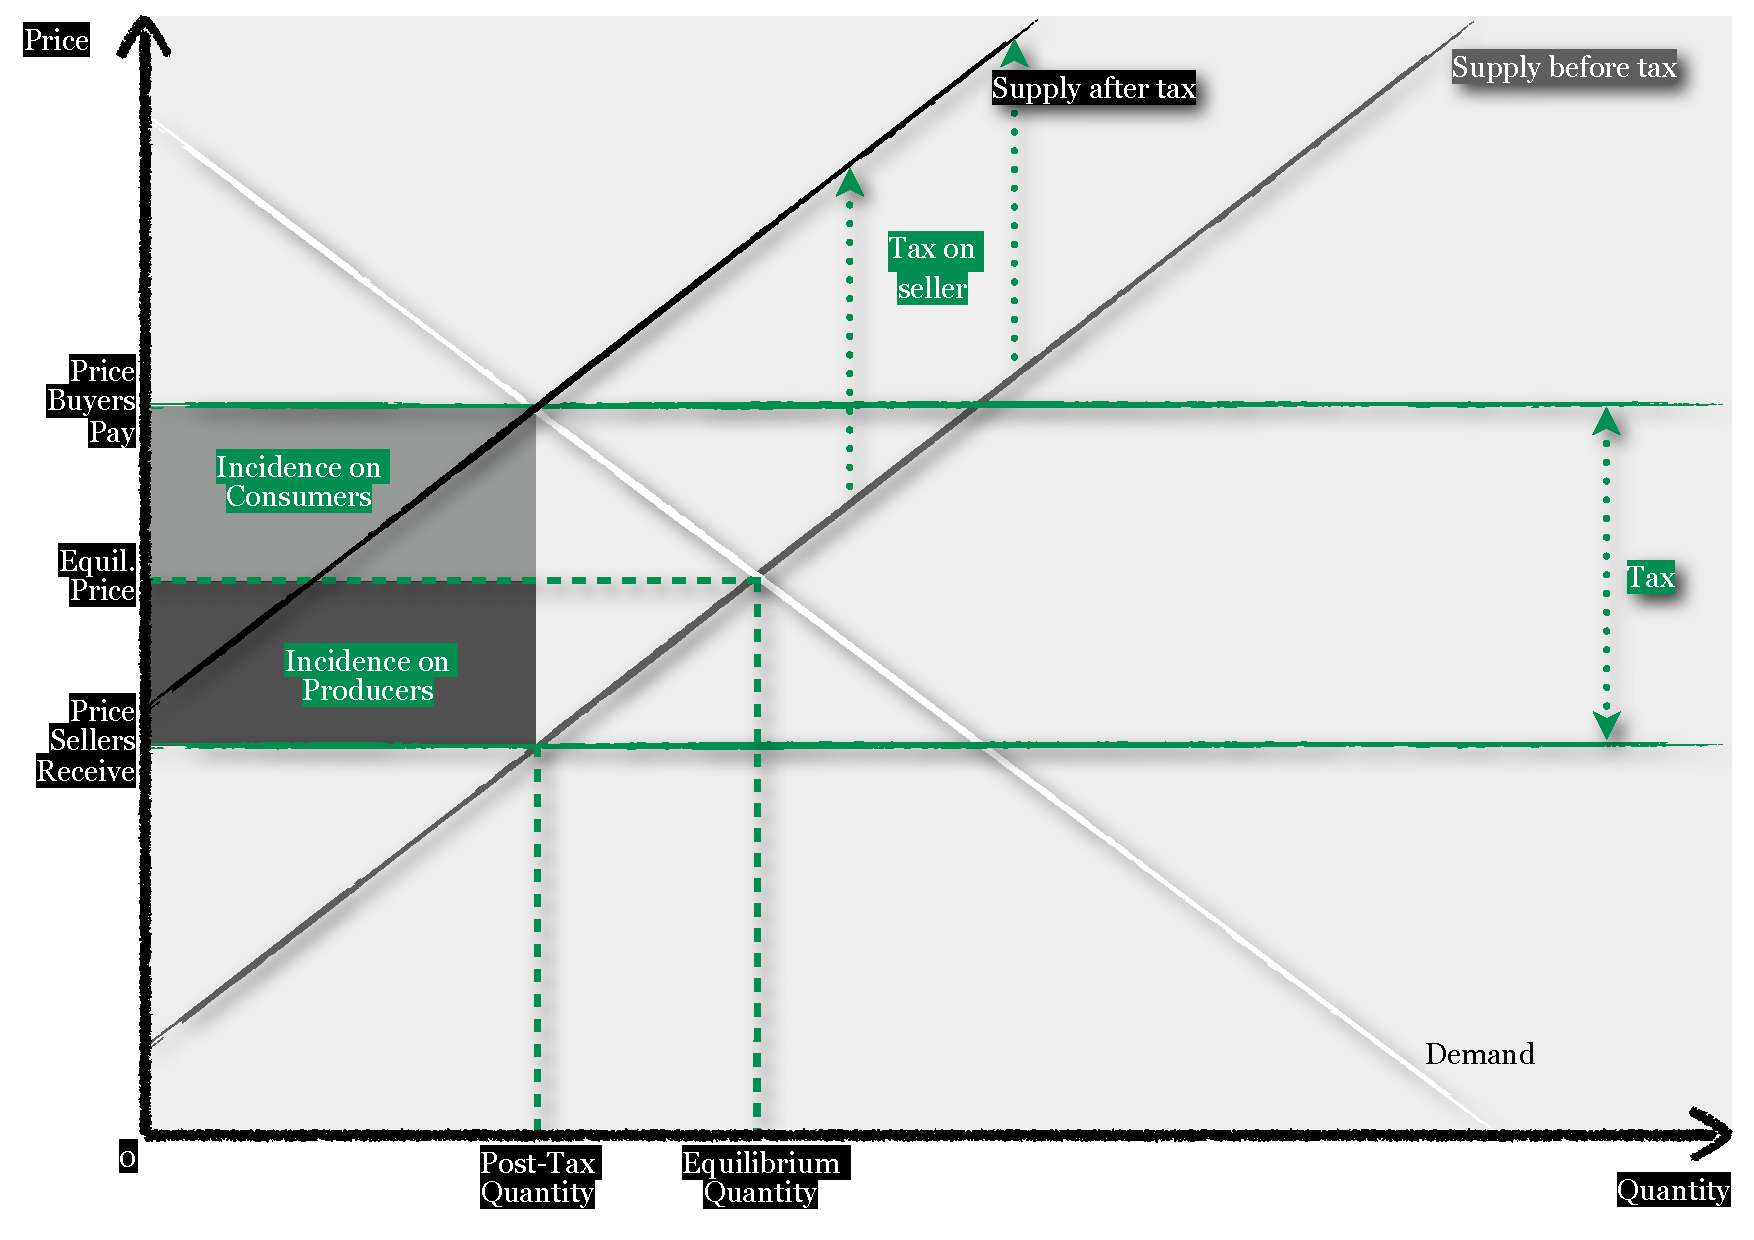
\includegraphics[width=1\textwidth]{same-incidence}
	\caption[Incidence of a Tax on Suppliers with Unit-Elastic Supply and Demand]{The Incidence of a Tax on Suppliers with Same Elasticities for Producers and Consumers}
	\label{fig:same-incidence}
\end{figure}

Taxation is always an \hyperref[sec:market-vs-command]{intervention in a market activity} (p.~\pageref{sec:market-vs-command}).
The incidence of a tax is borne by all parties to these market exchanges in proportion to their relative price elasticities of demand and supply, respectively, as shown in \autoref{fig:different-incidence} (p.~\pageref{fig:different-incidence}).
Whoever can cheaply exit or substitute the taxed market exchange dodges most of the tax:
because these price elastic suppliers \emph{would} quickly cut their quantity supplied at lower prices, they can extract relatively high prices from buyers.
Buyers, in this example, cannot cheaply exit or substitute the taxed market exchange:
they \emph{would} hardly be able to cut their quantity demanded in response to higher prices.
At the post-tax equilibrium, buyers foot most of the tax.

 \begin{figure}[htbp]
	\centering
	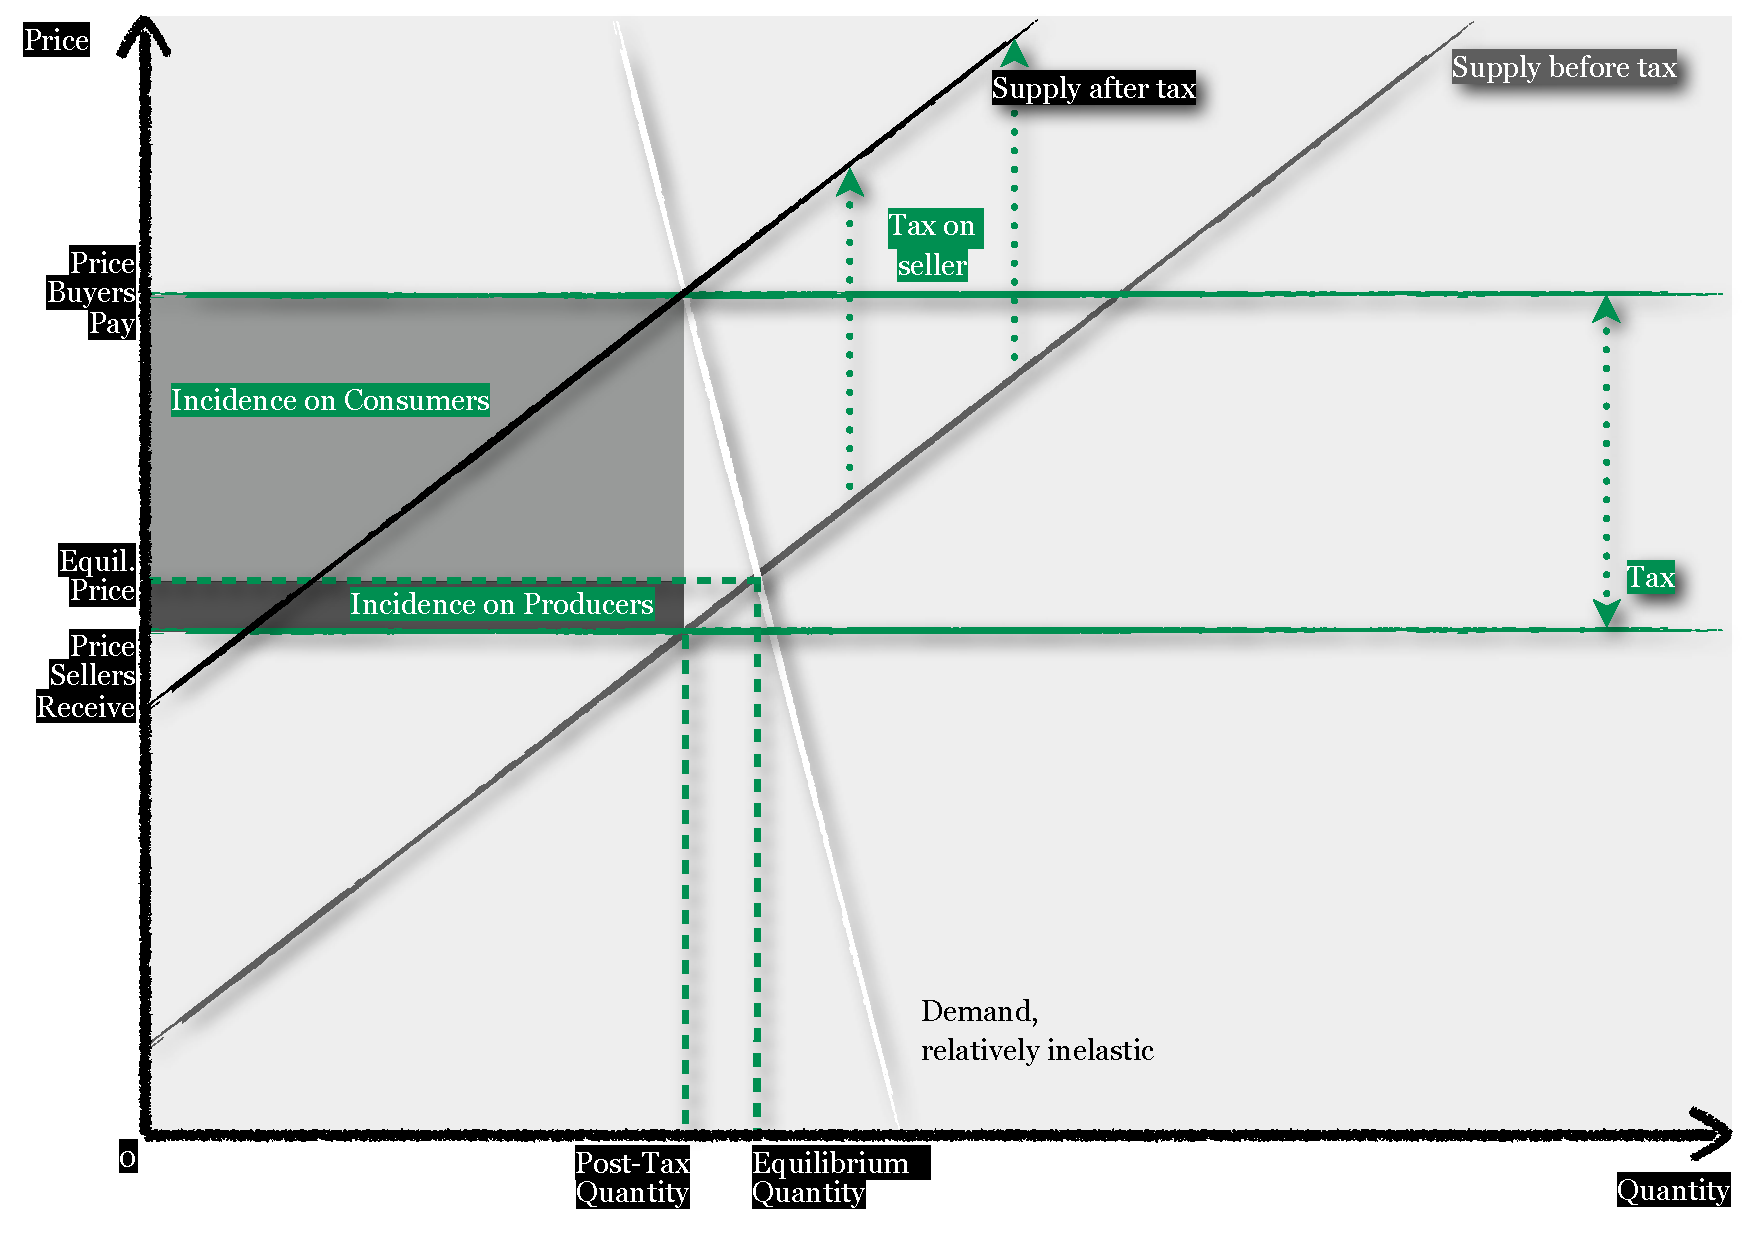
\includegraphics[width=1\textwidth]{different-incidence}
	\caption[Incidence of a Tax on Suppliers with Relatively Inelastic Demand]{The Incidence of a Tax on Suppliers with Relatively Less Elastic Demand}
	\label{fig:different-incidence}
\end{figure}

In the real world, relative price elasticities of demand and supply in many markets are unknown and would be difficult to ascertain.
\footnote{
	It is usually assumed that incidence applies only to \emph{indirect} taxes such as \gls{VAT} and \gls{CIT}.
	I find this limited application of incidence implausible.
	The concept remains applicable for \emph{direct} taxes, including \gls{PIT} and \gls{WT}, too.

	A \gls{PIT} on labor incomes, for instance, may partially fall on employers when labor markets are very tight:
	tax-depressed worker supply may cause employers to pay more.
	Even a \gls{WT} may fall on people other than the owners when demand for their collateral is sufficiently inelastic:
	interest rates may rise when private capital becomes less abundant.
}
Elasticity of demand and supply depends on many factors, including the availability of substitutes (for example,, margarine for butter) as well as the mobility and specificity of factors (for example, immobile, specific typewriter factory vs mobile, unspecific car rental).

Therefore, to fairly and effectively redistribute between natural persons, government must tax market interactions where the relative price elasticities of demand and supply can be easily known.
This is often the case for very broad categories of market exchanges, such as labor (\gls{Payroll}) or consumption (\gls{VAT}):
\footnote{
	A proportional \gls{Payroll} is actually equivalent to a \gls{VAT} in its incidence.
	A \gls{Payroll} taxes (only) labor income before it is spent (prepaid), a \gls{VAT} taxes (only) labor income after it is spent (postpaid).
}
people cannot substitute working \emph{somewhere} or employing \emph{someone}, they cannot avoid to buying or selling \emph{something}.
\footnote{
	Saving is a third alternative if you subscribe to a \emph{\gls{Y2C}}:
	when you consider returns on capital a genuine \emph{change} in welfare, you can substitute present spending for \emph{more} future spending.

	If, instead, you believe in a \emph{\gls{OSN}}, returns on capital are just compensation to risk, uncertainty and delayed pleasure:
	welfare is \emph{postponed}, but not changed.
	Consequently, under a \gls{OSN}, you can only substitute current consumption for same future consumption, and have no alternative but to spend your money at some point.

	For a summary of the savings norm debate see \cite{Held2010a} or, in the brilliant original, \cite[819]{McCaffery2005}.
}
The price elasticities for demand and supply in these broadly defined markets are small and similar.

In the closed economy, government can effectively tax broad categories of market exchanges, such as consumption.
\footnote{
	I use consumption and, broadly equivalently, labor as examples here because unlike income taxation (\gls{PIT}), they do not require me to decide on a savings norm (\gls{Y2C} or \gls{OSN}).
	Both norms are unattractive in the extremes and only a \gls{PCT} can resolve the tension (\citealt{Held2010a}).

	Still, it is important to point out that, no matter the savings norm, savers in a closed economy have limited or no alternative to investing at home.
	Therefore, the incidence of a \gls{PIT} will also be relatively well-defined in a closed economy.
}
By definition, economic activity does not extent beyond the borders of the closed economy, and there can therefore be no substitution to, for example, spending at home.

\subparagraph[Tax Efficiency]{Minimal Market Distortions, Welfare Losses.} \phantomsection \label{sec:minimal-DWL}
When government taxes a market exchange, buyers and sellers may react in ways that reduce overall welfare.

When the post-tax price of the transaction is higher than the buyers utility or the sellers cost, they exit the market.
Their otherwise pareto-improving exchange does not occur, as shown in \autoref{fig:DWL} (p.~\pageref{fig:DWL}).
Government also gains no revenue from these non-occurring transactions.
Everybody loses.
The sum total of these losses is known as the \gls{DWL} of taxation (areas C, E in figure \href{fig:DWL}).
An efficient tax minimizes \gls{DWL} for maximum revenue (areas B, D).

\begin{figure}[htbp]
	\centering
	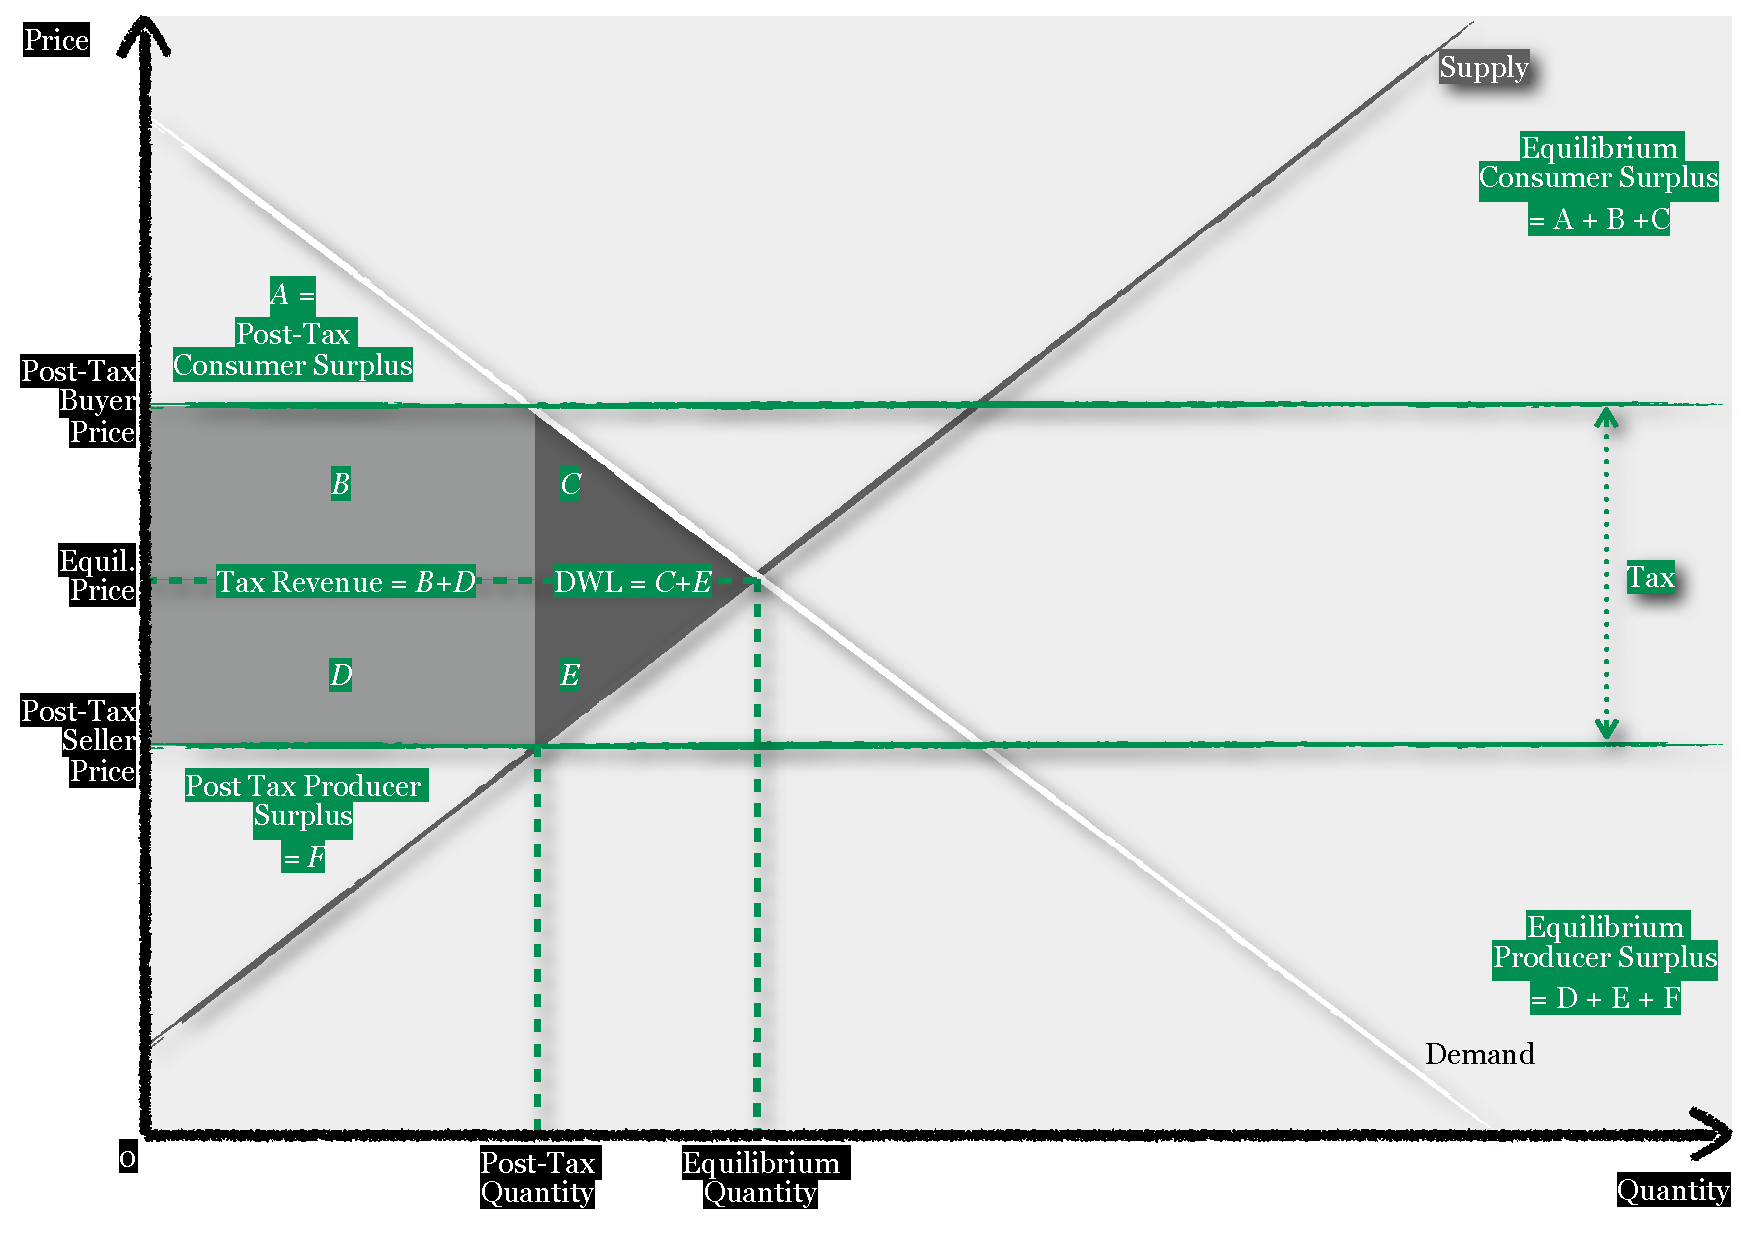
\includegraphics[width=1\textwidth]{dwl.pdf}
	\caption[Deadweight-Loss of a Tax with Unit-Elastic Supply and Demand]{The \gls{DWL} of a Tax with Unit-Elastic Supply and Demand}
	\label{fig:DWL}
\end{figure}

This ratio of tax revenue to \gls{DWL} --- much like the \hyperref[sec:well-determined-incidence]{effective incidence of a tax} (p.~\pageref{sec:well-determined-incidence}) --- depends on the price elasticities of supply and demand.
The more inelastic supply and demand, the smaller the \gls{DWL} for any given tax rate, as shown in \autoref{fig:smaller-DWL} (p.~\pageref{fig:smaller-DWL}).
If buyers and sellers cannot easily cease their welfare-improving exchanges, they will continue to trade when taxed.
A tax on such a market will not distort or depress market activities.

\begin{figure}[htbp]
	\centering
	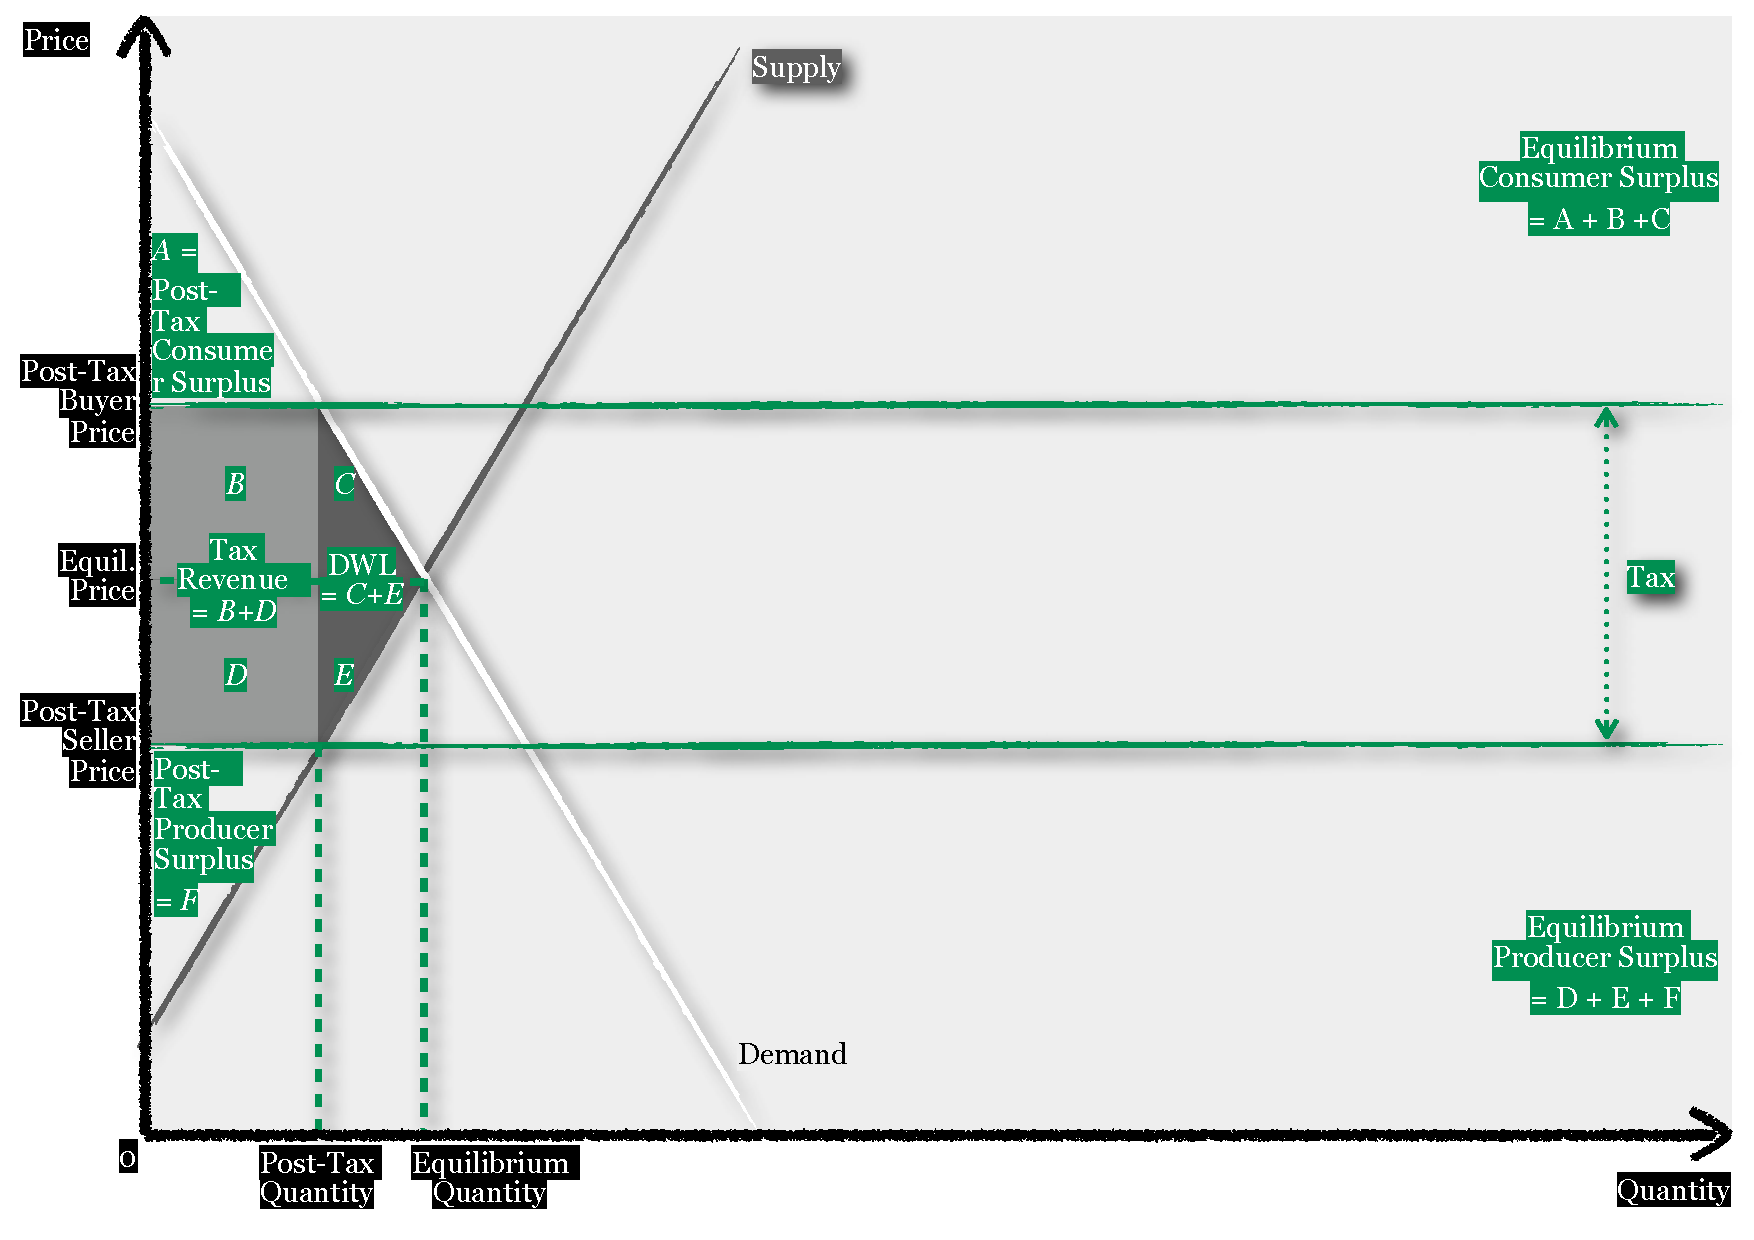
\includegraphics[width=1\textwidth]{smaller-DWL}
	\caption[Deadweight-Loss of a Tax with Inelastic Suppy and Demand]{The Deadweight-Loss of a Tax with Inelastic Supply and Demand}
	\label{fig:smaller-DWL}
\end{figure}

The price elasticities of demand and supply are, again, a hard, empirical question.
As discussed above, supply and demand in broad categories of market exchanges, such as all domestic consumption (\gls{VAT}) or all domestic labor (\gls{Payroll}) are relatively inelastic, and the \gls{DWL} of such taxes is likely to be small in a closed economy.

Still, \glspl{DWL} of taxation may abound, even in closed economies.
In mixed economies, the market for low-wage labor is particularly vulnerable to large \gls{DWL}s.
Welfare state governments  \hyperref[sec:distribution]{may find it necessary to give handouts} to people who earn too little to maintain a socially acceptable standard of living (p.~\pageref{sec:distribution}).

In this scenario, taxation of low-wage labor has two related, negative effects.
\footnote{
	As explained in the above, both a \gls{Payroll} and a \gls{VAT} burden low-wage labor.
}
\begin{enumerate}
	\item Taxation raises the effective cost of living for low-wage earners:
for each euro they earn on the market, they can afford a lower, real standard of living.
	\item If people can apply for handouts, their supply of labor may become perfectly price elastic, when market incomes are close to welfare incomes.
	If they could earn less on the market, than by collecting welfare, low-wage workers may be forced to exit the labor market:
	a large \gls{DWL} ensues.
	\footnote{
		In this extreme, unlikely case, the \gls{DWL} of a welfare handout is equivalent to the \gls{DWL} of a price floor on labor at the same level.
	}
	Any tax on low-wage labor will only increase the \gls{DWL}:
	for every euro of wages taxed, more people will be pushed outside the (official) labor market.
	\footnote{
		People leaving the labor market in this scenario has nothing to do with laziness.
		The legislated minimum standard of living is after all considered minimally acceptable.
		People who opt for welfare instead of poorly paid work may not have a choice.
	}
\end{enumerate}

In the closed economy, government can minimize the tax burden on low-wage labor by relying more on progressive taxes, including a \gls{PIT}, instead of proportional taxes (\gls{VAT}, \gls{Payroll}).


\subsection[Monetary Policy]{The Means of Monetary Policy} \label{sec:monetary}
Government provides the economy with legal tender to serve as \begin{inparaenum}[1)]
	\item a medium of exchange,
	\item a unit of account and
	\item a store of value.
\end{inparaenum}
Only government can do this, because supplying money is a \hyperref[sec:natural-monopoly]{natural monopoly} (p.~\pageref{sec:natural-monopoly}).
To avoid the \hyperref[sec:price-stability]{costs} (p.~\pageref{sec:price-stability}) and  \hyperref[sec:distributive-effects-of-inflation]{arbitrary redistribution} (p.~\pageref{sec:distributive-effects-of-inflation}) of de- or inflation,
governments should be devoted to price stability.

They set that quantity of money where it equilibrates with variable money \emph{demand} at stable prices.
The demand for money, in turn, is determined by the output of the economy.
\footnote{
	This very brief account follows the \emph{quantity} theory of money.
	Competing theories are discussed in the below.
}

\paragraph[Tools]{Tools.} Government extends or contracts the supply of money to meet a quantity, interest rate (US) or inflation rate (Bundesbank) target.
Fiat money is supplied in one of two ways:
\footnote{
	If for no other reason, fiat money would be preferable to intrinsically valuable moneys \emph{because} governments can adjust its supply to output in the long run and at little cost.
	By contrast, specie moneys are costly to extract and their supply changes arbitarily on new discovery.

	The futility of a gold-based economy is aptly summarized by investor Warren Buffett:
	\begin{quote}
		\emph{``[Gold] gets dug out of the ground in Africa, or someplace.
		Then we melt it down, dig another hole, bury it again and pay people to stand around guarding it.
		(\ldots)
		Anyone watching from Mars would be scratching their head.''}
		\\*
		--- Warren Buffett
	\end{quote}
}
\begin{enumerate}
	\item Government creates \emph{base money} by \begin{inparaenum}[a)]
		\item buying government bonds (\gls{OMO}) or
		\item other financial assets (\gls{QE}) from private holders who receive legal tender out of thin air
		\footnote{
			Actually, the balance sheet of the central bank records the acquired bond as an asset, and the currency as a liability.
		}
		in return.
		\footnote{
			Central banks are customarily barred from buying government bonds directly from government to increase transparency.
			By buying government bonds from a middlewoman, central banks can still ``print money''.
		}
		Central banks can also
		\item lend money to financial institutions at a set rate (discount window rate).
	\end{inparaenum}
	\item Government stimulates the multiplication of \emph{broad money} in the fractional reserve banking system by lowering the reserve requirements for private banks.
\end{enumerate}

 \begin{figure}[htbp]
	\centering
	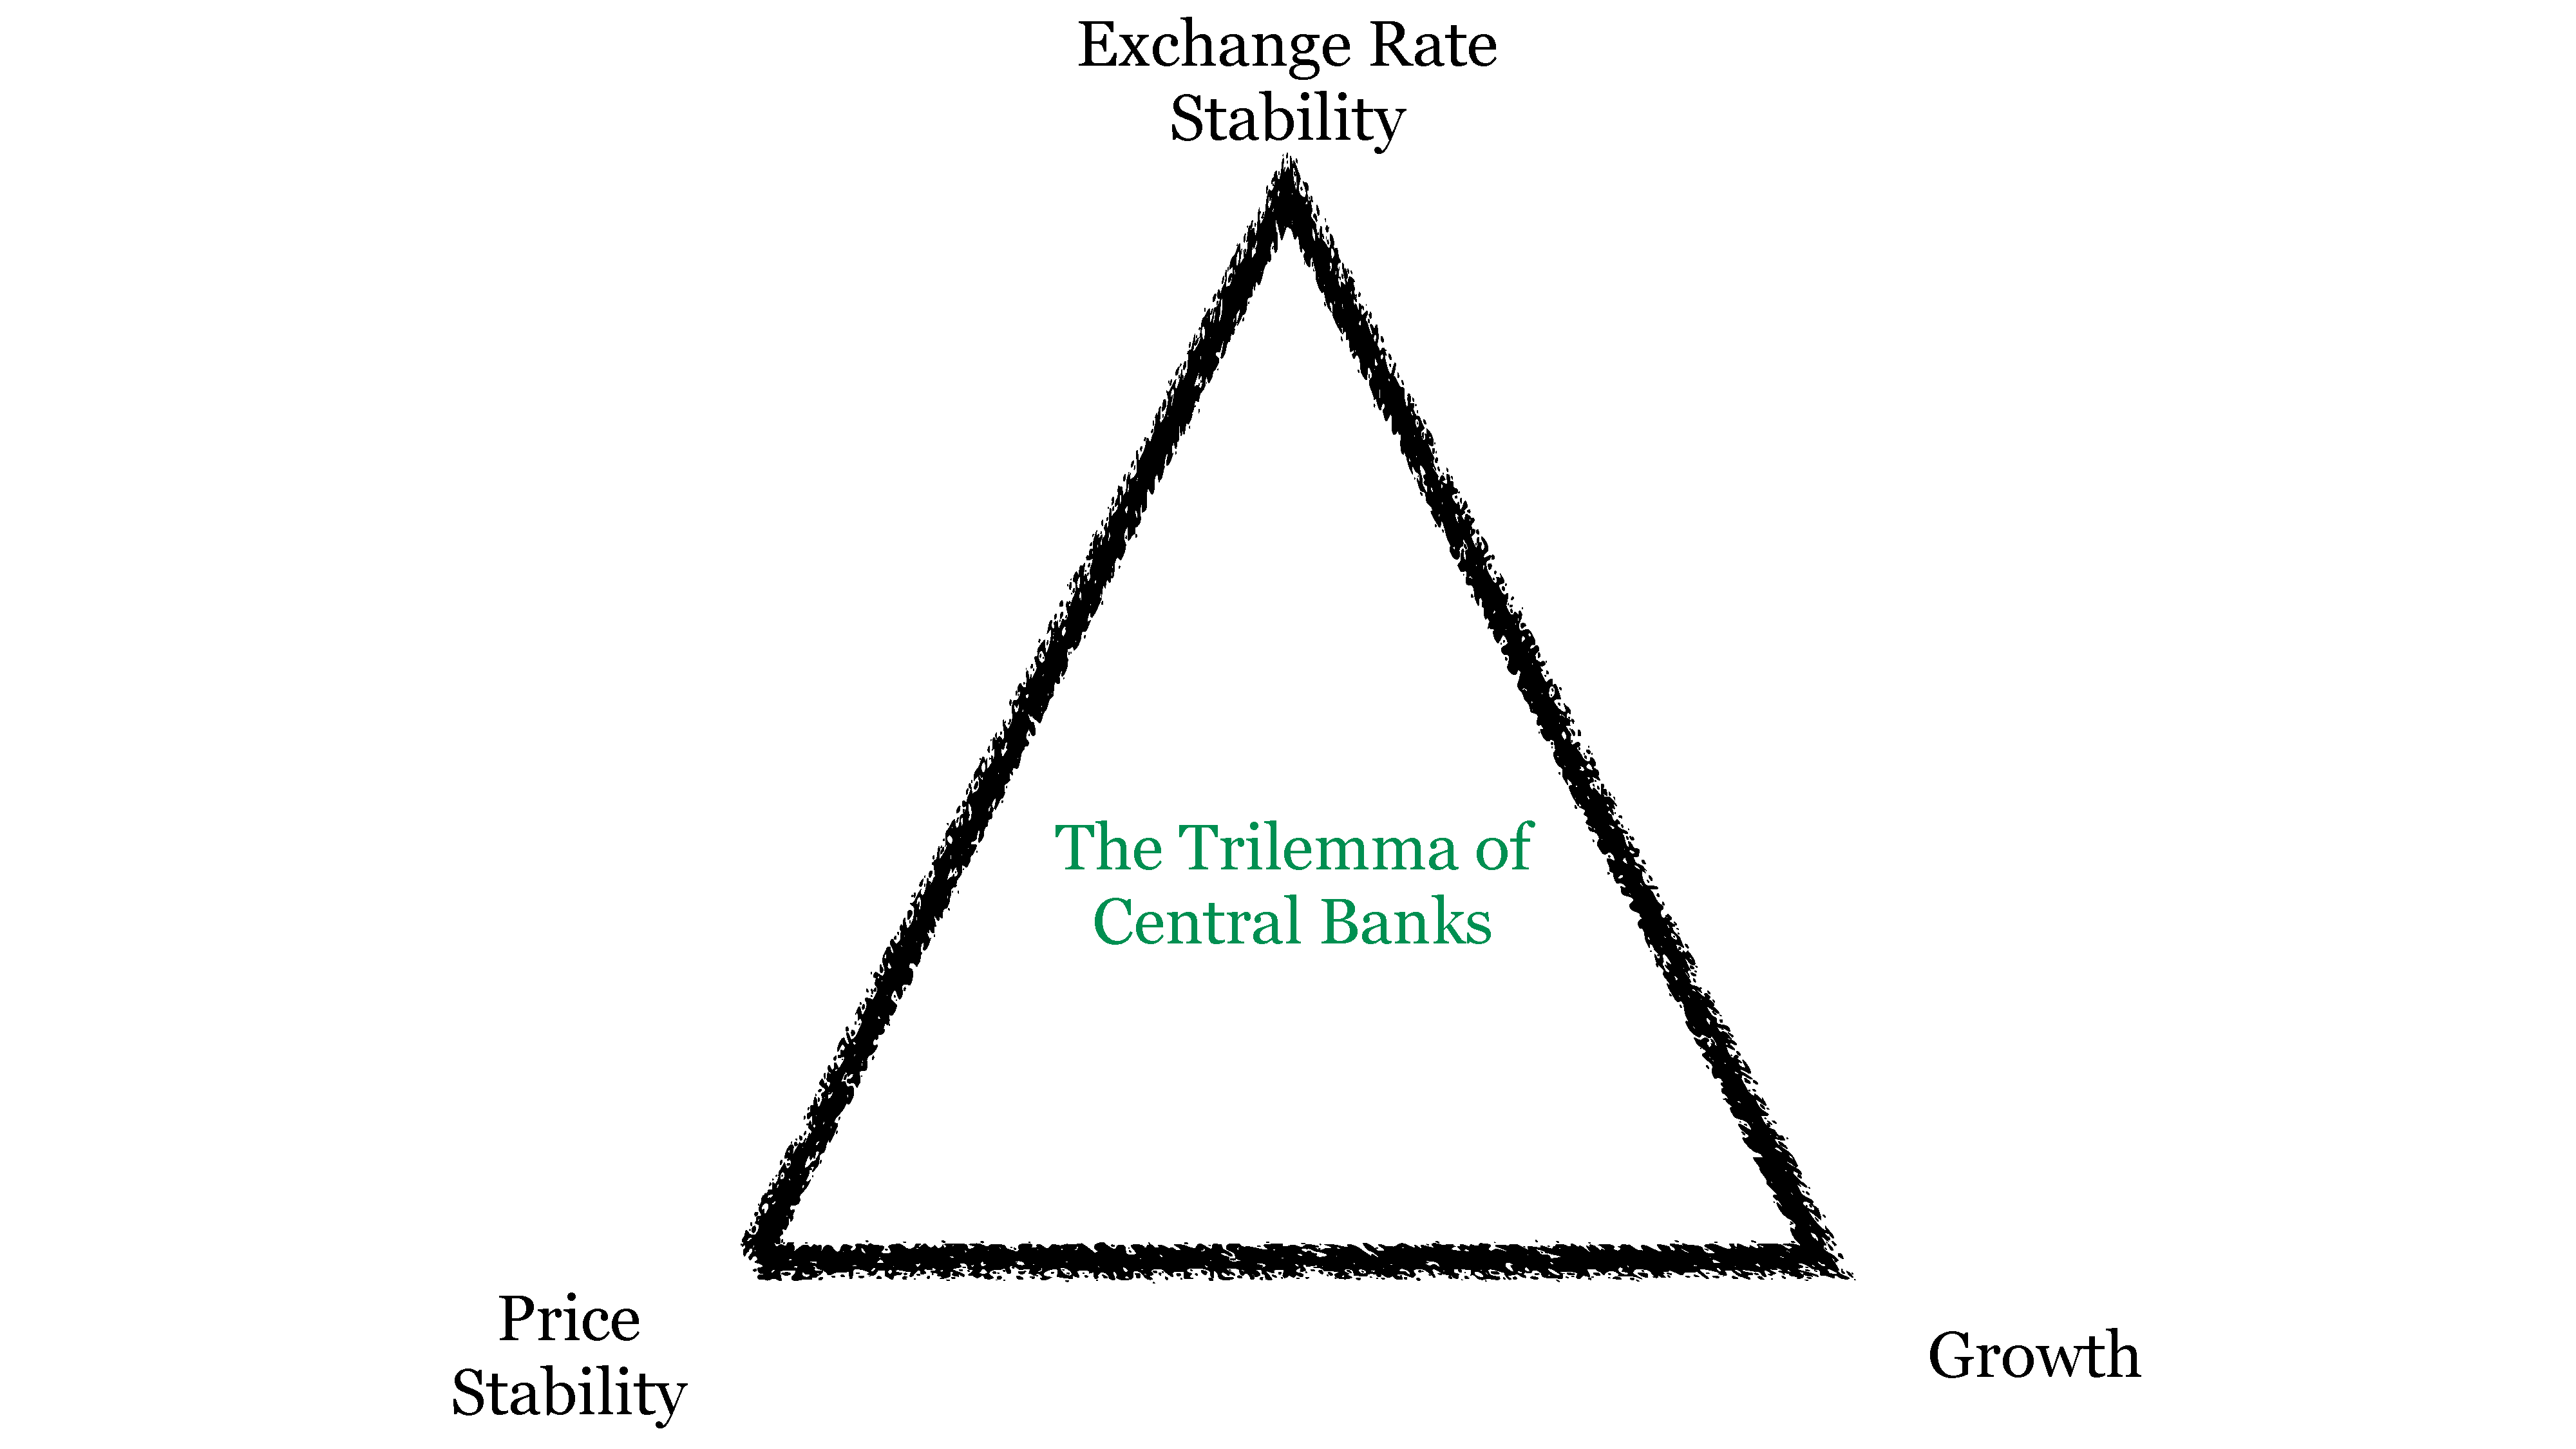
\includegraphics[width=1\linewidth]{triangle-cb}
	\caption{The Policy Trilemma of Central Banks}
	\label{fig:triangle-cb}
\end{figure}

\paragraph[Role]{Role.} %This section is horseshit.
The impact of monetary policy on the real economy is, of course, incompletely understood and highly controversial.
I do not need to recapitulate these controversies here (for a recent review, see \citealt{Wapshott2011}).
I note two hopefully uncontroversial points:

\begin{enumerate}
	\item \emph{Monetary Neutrality.} \label{itm:monetary-neutrality} Following the classical dichotomy, \emph{nominal} economic variables, such as the price level, do not matter in the long run.
The prosperity of an economy is determined by its level of technology, human capital and physical capital --- not by the amount of intrinsically worthless currency in circulation.

	On this ultimate end of monetary policy, Monetarists and Keynesians can probably agree:
good money stays out of way of the real economy to let actual output track the long-term growth path of the economy.

	\item \label{itm:empirical-macroeconomics} \emph{An Empirical Question.}
	Different monetary theories follow from different assumptions about human behavior:

	%\footnote{\label{i:empirical-macroeconomics}
%		Indeed, monetary policy seems greatly concerned with mass psychology, or \emph{open-mouth-operations} in addition to \gls{OMO}s.
%		For example, according to rational expectations theory, it is important for a central bank to \emph{appear} credibly tough on inflation to keep inflation down.}.

	\begin{description}
		\item[Keynesians] believe that market participants are swayed by changes in nominal variables.
		As a result, the prices for goods and services and factor prices (especially wages) do not equilibrate promptly or perfectly.
		Self-reinforcing (debt-deflation) crises of excess supply and depressed demand may result \citep{Fisher1933}.
		The state can smooth out resulting aggregate fluctuations in output by altering the money supply.
		\item[Monetarists] believe that market participants are fairly rational and will consider expectations of future inflation (and taxes) in their current decisions.
		As a result, prices for goods and services and factor prices, especially wages, equilibrate quickly and keep the economy on its long-term growth trajectory.
		State intervention in the business cycle or the money supply are unnecessary and ineffective.
		\footnote{
			They are unnecessary according to \glsfirst{RBCT}.
		}
		\footnote{
			They are ineffective according to the policy ineffectiveness proposition.
		}
	\end{description}

	Determining our irrational \emph{animal spirits} \citep{Keynes1936} is an empirical question best left to cognitive psychology, behavioral economics and related fields (recently \citealt{Akerlof2010}, see \autoref{itm:empirical-macroeconomics}, p.~\pageref{itm:empirical-macroeconomics})
	``Keynes v.
Hayek'' \citep{Wapshott2011} need not be a normative struggle, but a pragmatic balance based on empirical evidence.
	Whichever policy stabilizes economic output along the long-term growth trajectory is best.

	If ever there was a policy that should be judged on consequentialist terms, it is monetary policy.
\end{enumerate}

Because monetary dynamics \emph{do not} and \emph{should not} matter to our `household with a cast of billions' I can refer the issue to empirical clarification and need not entertain it further here.
Suffice it to remind us that government should set that quantity of money where it equilibrates with variable money demand at stable prices.
The rest is empirical details.

\section[Trade-Offs]{Trade-Offs of the Mixed Economy \textsuperscript{\ref{fn:also-in-europe}}} \label{sec:trade-offs}

%needs quote

Given its conflicting \hyperref[sec:ends]{ends} (p.~\pageref{sec:ends}) the mixed economy can arrange its \hyperref[sec:means]{means} (p.~\pageref{sec:means}) to make at least two basic trade-offs.
\begin{enumerate}
	\item \emph{Command vs.\ Exchange.} It can organize more or less production and distribution by command instead of exchange.
	\item \emph{Consumption vs.\ Saving.} It can defer more or less of current consumption to the future.
\end{enumerate}

We can look at these trade-offs by \hyperref[sec:by-expenditure]{expenditure} (p.~\pageref{sec:by-expenditure}) and by \hyperref[sec:delta-net-worth]{changes in net worth} (p.~\pageref{sec:delta-net-worth}) of the entire economy.

\paragraph[By Expenditure]{By Expenditure.} \phantomsection \label{sec:by-expenditure}
A mixed economy can devote its resources (expenses) to public or private, investment and consumption goods.
The four expenditure components and revenue flows are plotted on a two-dimensional coordinate space of the mixed economy in \autoref{fig:coordinate-space} (p.~\pageref{fig:coordinate-space}).
I provide (very roughly) equivalent macroeconomic variables as \hyperref[tab:GDP-Comp-Exp]{components of GDP by expenditure} in \autoref{tab:GDP-Comp-Exp} (p.~\pageref{tab:GDP-Comp-Exp}).
\footnote{
	\gls{GDP} and its macroeconomic components, while commonly reported, falls short of a comprehensive account of the economy.

	Rather than a measure of prosperity, it indicates market value level of economic \emph{activity}.
	Roughly, \gls{GDP} is to prosperity, as a corporation's cash flow statement is to its income statement.
	\gls{GDP} growth and positive cash flows are a necessary, but not a sufficient condition to prosperity.

	\gls{GDP} does not measure changes in net worth as an income statement would:
	for example, an earthquake (or nuclear power disaster, or both) can raise \gls{GDP} because of reconstruction \emph{activities}, even if it actually wiped out \emph{assets}.
	\gls{GDP} also excludes environmental degredation or use of natural resources.

	Lastly, \gls{GDP} falls short, because it records only activity with a market value;
	economic activity in the household or family are not included, as are social costs or utility of market activities (externalities).
}

\begin{landscape}
 \begin{figure}[htbp]
	\centering
	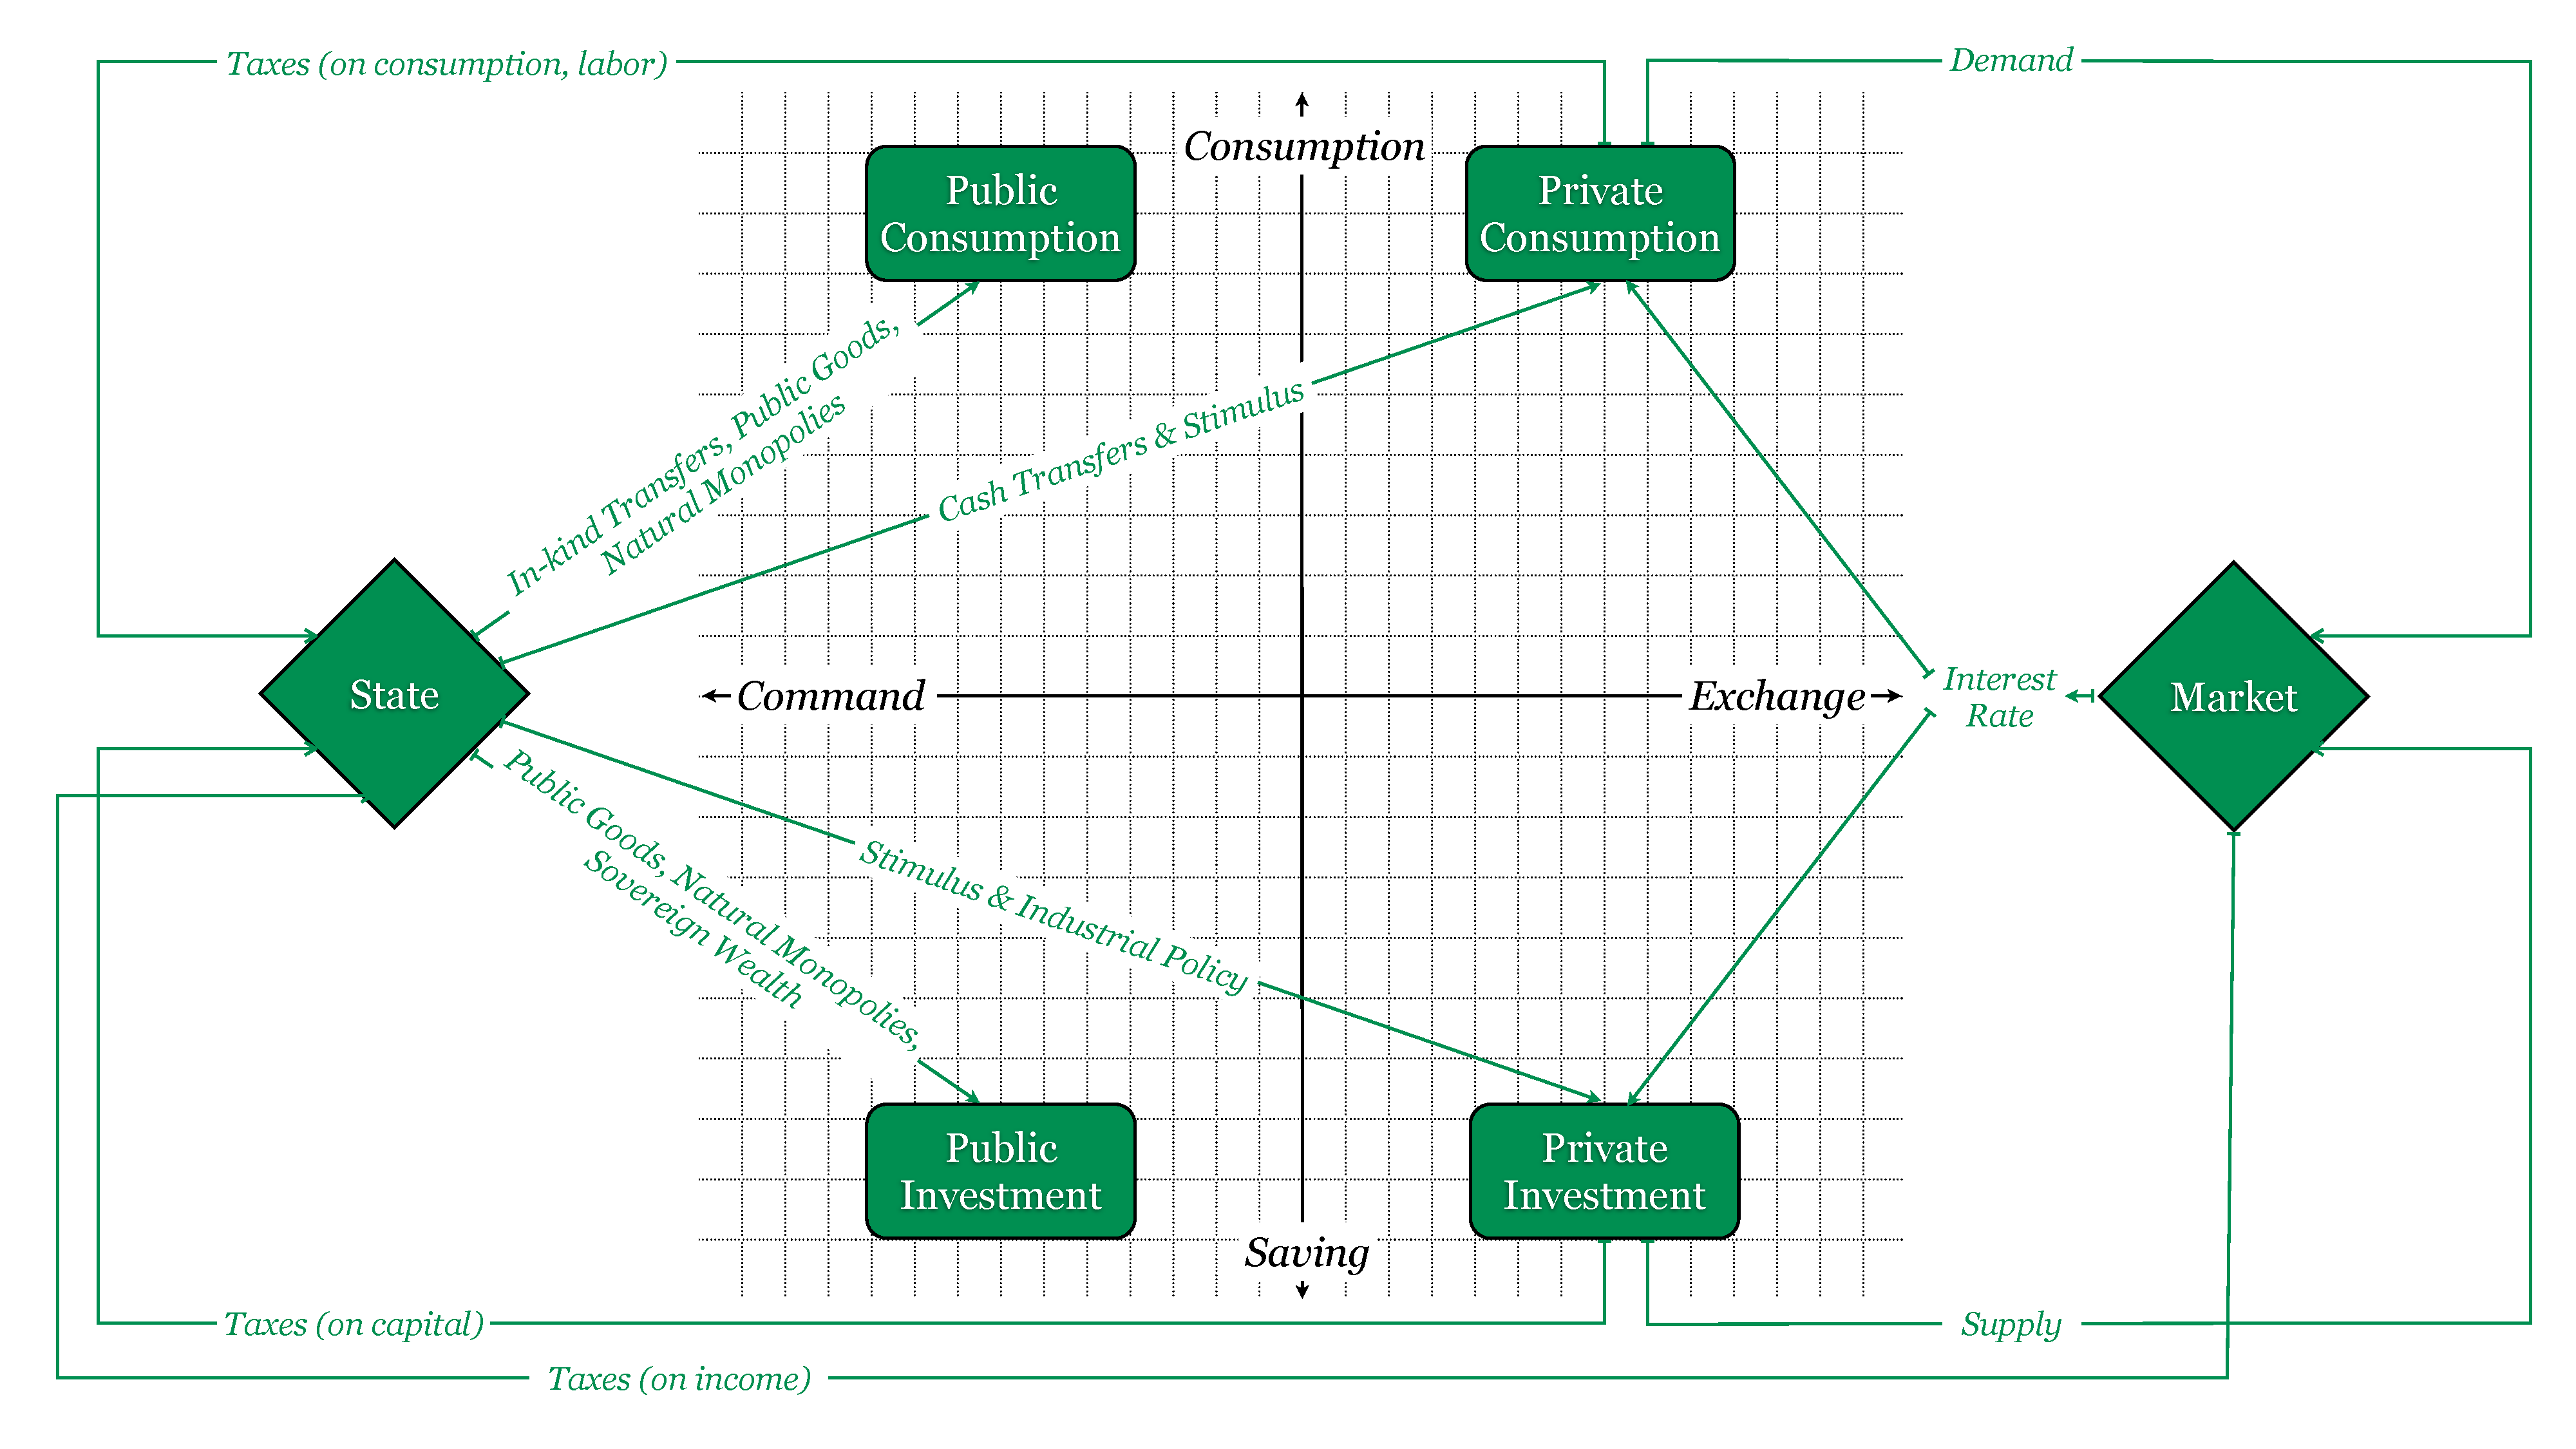
\includegraphics[width=1\linewidth]{coordinate-space}
	\caption{Coordinate Space of the Mixed Economy}
	\label{fig:coordinate-space}
\end{figure} %add squalor etc.
%to the coordinate space
\end{landscape}

\begin{figure}[htbp]
	\centering
	%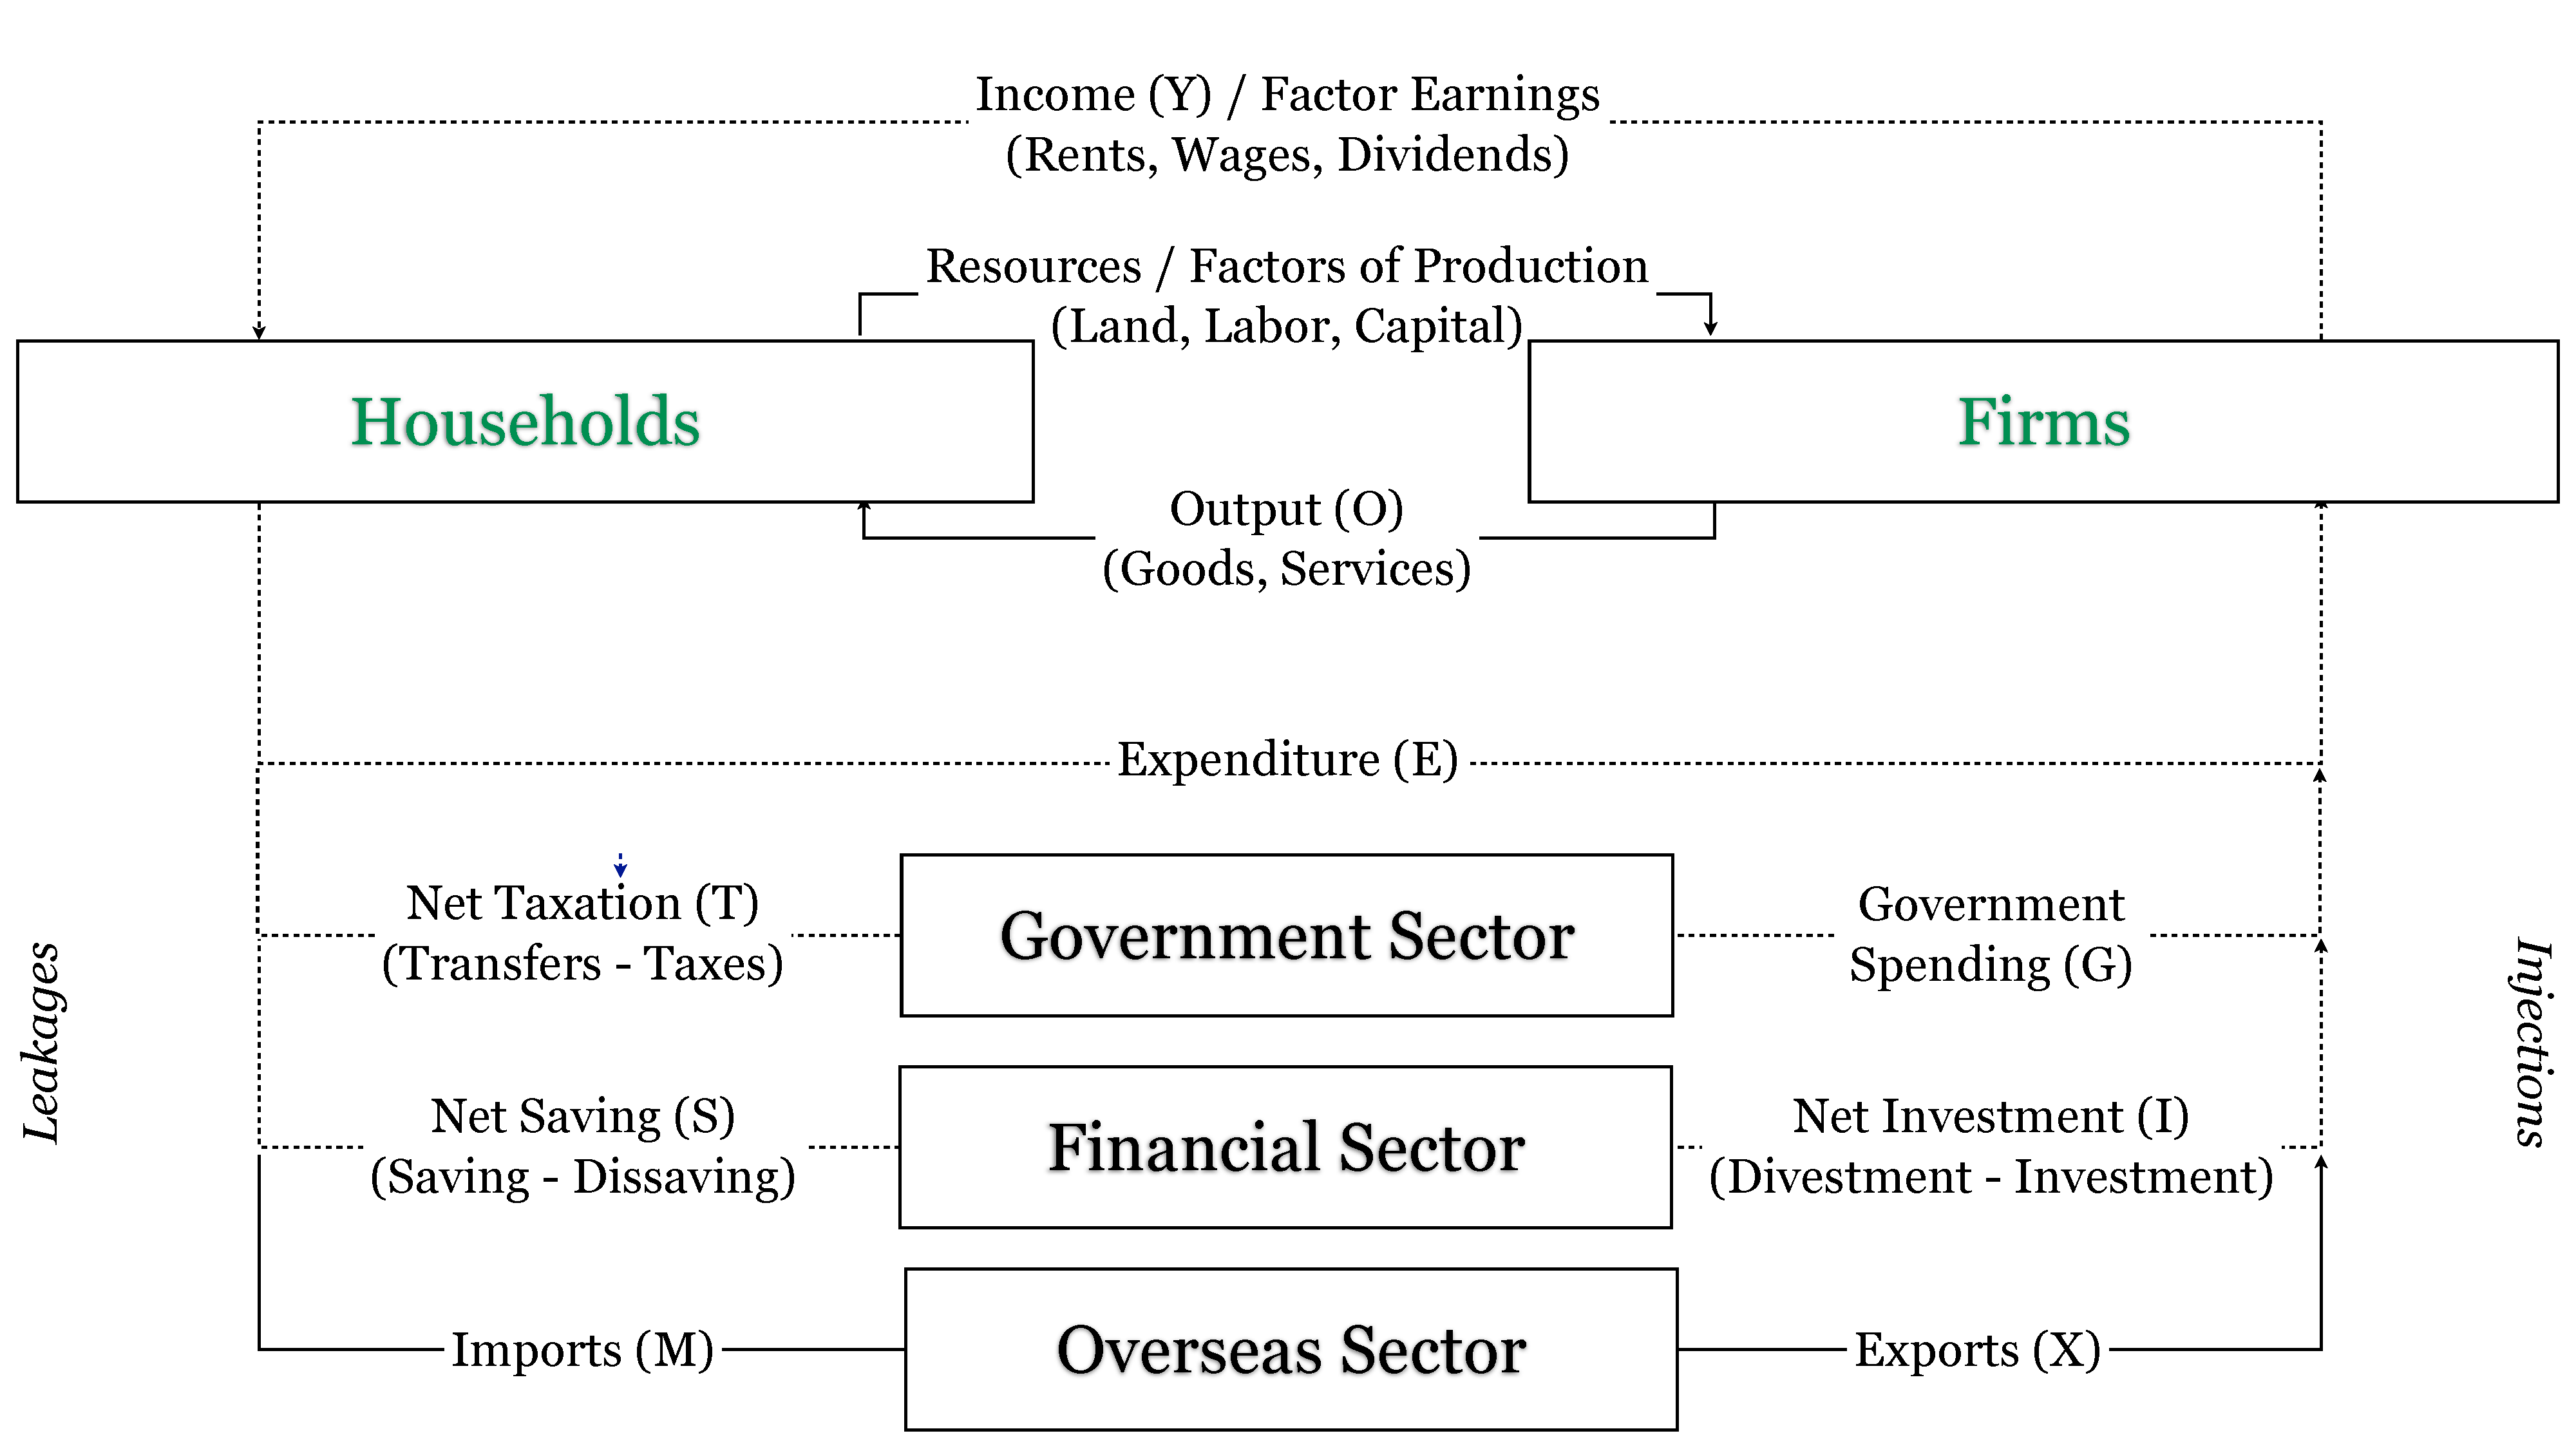
\includegraphics[width=1\textwidth]{circular-flow.pdf}
	\caption[Circular Flow in the Economy]{Circular Flow of Income in the Economy}
	%\begin{flushleft}
	%	\scriptsize{some text.}
%	\end{flushleft}
	\label{fig:circular-flow}
\end{figure}
%I have not explained the prior graph yet!

%add somewhere a section on why saving doesn't lead to low demand.
%BASTARD KEYNESIANISM.
%Gotcha.
\subparagraph[Save More or Less]{Save/Consume More or Less.} Government increases the private savings rate by taxing consumption (instead of income), encouraging investment (factory) through industrial policy or other fiscal stimulus and increases public saving by putting net tax revenue into durable public goods (basic research), natural monopolies (a bridge) or \glsplural{SWF}.

Steering in the opposite direction, government increases private consumption by cash transfers, fiscal stimulus and public consumption by handing out in-kind benefits (school milk), or providing short-term public goods (fireworks) and natural monopolies.
The saving-consumption trade-off roughly expressed in the gross savings rate in \autoref{tab:GDP-Comp-Exp} (p.~\pageref{tab:GDP-Comp-Exp}).
\footnote{
	GDP-related metrics fall short, again:
	\gls{GFCF} and consequently the gross savings rate does not include capital depreciation.
	It also does not include real dissavings on goods without a market value, such as the population growth rate or environmental quality.

	Consequently, gross savings rates may be overstated in existing accounts.
}

	% why aren't public budgets documented like the budgets of private firms, including a full balance sheet?
%how is this ENRON accounting even possible?

\subparagraph[Exchange-Command Mix]{More or Less Government/Market} Government sets the exchange-command mix of the economy by taxing more or less of economic output, and commissioning public investment and consumption from the revenue.
The exchange-command mix is (roughly) expressed in the public expenditure quota in \autoref{tab:GDP-Comp-Exp} (p.~\pageref{tab:GDP-Comp-Exp}).

\subparagraph[Optima]{How to Strike the Best Balance.} Welfare economics and the \hyperref[sec:ends]{ends} of a mixed economy (p.~\pageref{sec:ends}) suggests that there are one (or more) \emph{optima} in the balance between saving and consumption, between market and command.
These ends also bind each of the government interventions, such as providing a public good, to \emph{specific} justifications,
\footnote{
	Justifying a choice of the mixed economy does not mean that it can be reduced to a positive question.
	Ends and means such as redistribution may, and maybe should, remain contested.
}
such as a market failure in providing the public good.
Normatively, government \emph{should} not take an arbitrary position on \hyperref[fig:coordinate-space]{the coordinate space of the mixed economy} (\autoref{fig:coordinate-space}).

However, I should point out that \emph{positively}, government in a closed economy \emph{could} employ its \hyperref[sec:means]{means} to choose any of the possible trade-offs between consumption and saving, market and command economy.
	%does this table actually correspond to all the state jobs, or just some?

\subparagraph[Tax is Key]{Tax is Key.} Of these \hyperref[sec:means]{means} of the mixed economy, tax is the dominant tool.
To redirect resources between the four quadrants, government relies primarily on \hyperref[sec:fiscal]{taxation} (p.~\pageref{sec:fiscal}) rather than on \hyperref[sec:regulatory]{regulation} (p.~\pageref{sec:regulatory}) which has limited applications and \hyperref[sec:monetary]{money} (p.~\pageref{sec:monetary}) which is neutral in the long run.

\begin{landscape}%check this table again, very thorougly.
\begin{table}
	\caption{GDP Components by Expenditure in the Closed Economy}
	\label{tab:GDP-Comp-Exp}
	\small
	\begin{center}
	\renewcommand{\arraystretch}{1.5}
	\begin{tabular}{llccrr}
		\toprule
		& & \multicolumn{2}{c}{\emph{Ownership}} & &\\
		\cmidrule(r){3-4}
		& &\emph{Private} & \emph{Public}& &\\
		\midrule
		\multirow{2}{*}{\emph{}} & \emph{\gls{I}} & Factory,  \gls{RnD} & Bridge, basic research & \emph{$\sum=$\gls{GFCF}} & \multirow{2}{*}{\emph{$\frac{\gls{GFCF}}{\gls{GDP}}=$Gross Savings Rate}}\\
		& \emph{\gls{C}} & TV set, vacation & School milk, fireworks & \emph{$\sum=$\gls{FCE}}  \\
		\midrule
		& &\emph{$\sum=$($\gls{I}+\gls{C}$)} & \emph{$\sum=$\gls{G}
		\footnote{
			\Gls{GDP} also does not, as implied in \autoref{fig:coordinate-space} distinguish between public consumption and public investment, but lumps both together in \gls{G}.
		}}\\
		\cmidrule(r){3-4}
		& & \multicolumn{2}{c}{$\frac{\gls{G}}{\gls{GDP}}=$ Public expenditure quota} \\
		\bottomrule
	\end{tabular}
	\end{center}
\end{table}
\end{landscape}

\paragraph{By Changes in Net Worth} \phantomsection \label{sec:delta-net-worth} The same trade-offs of the mixed economy can also be understood as different changes in net worth.

As economies, firms and households save and consume, their net worth changes.
This truism is expressed in the Haig-Simons income identity:

\begin{equation} \label{eq:haig-simons}
			\text{Income}=\text{Consumption}+\Delta\text{Wealth}
\end{equation}

Or, trivially transformed:
\begin{equation} \label{eq:haig-simons-trade-off}
			\text{Savings}-\text{Dissavings}=\text{Income}-\text{Consumption}
\end{equation}

\autoref{fig:haig-simons-individual-collective} applies \autoref{eq:haig-simons-trade-off} to the savings trade-off of households, firms and government, including some examples.

\begin{figure}[htbp]
	\centering
	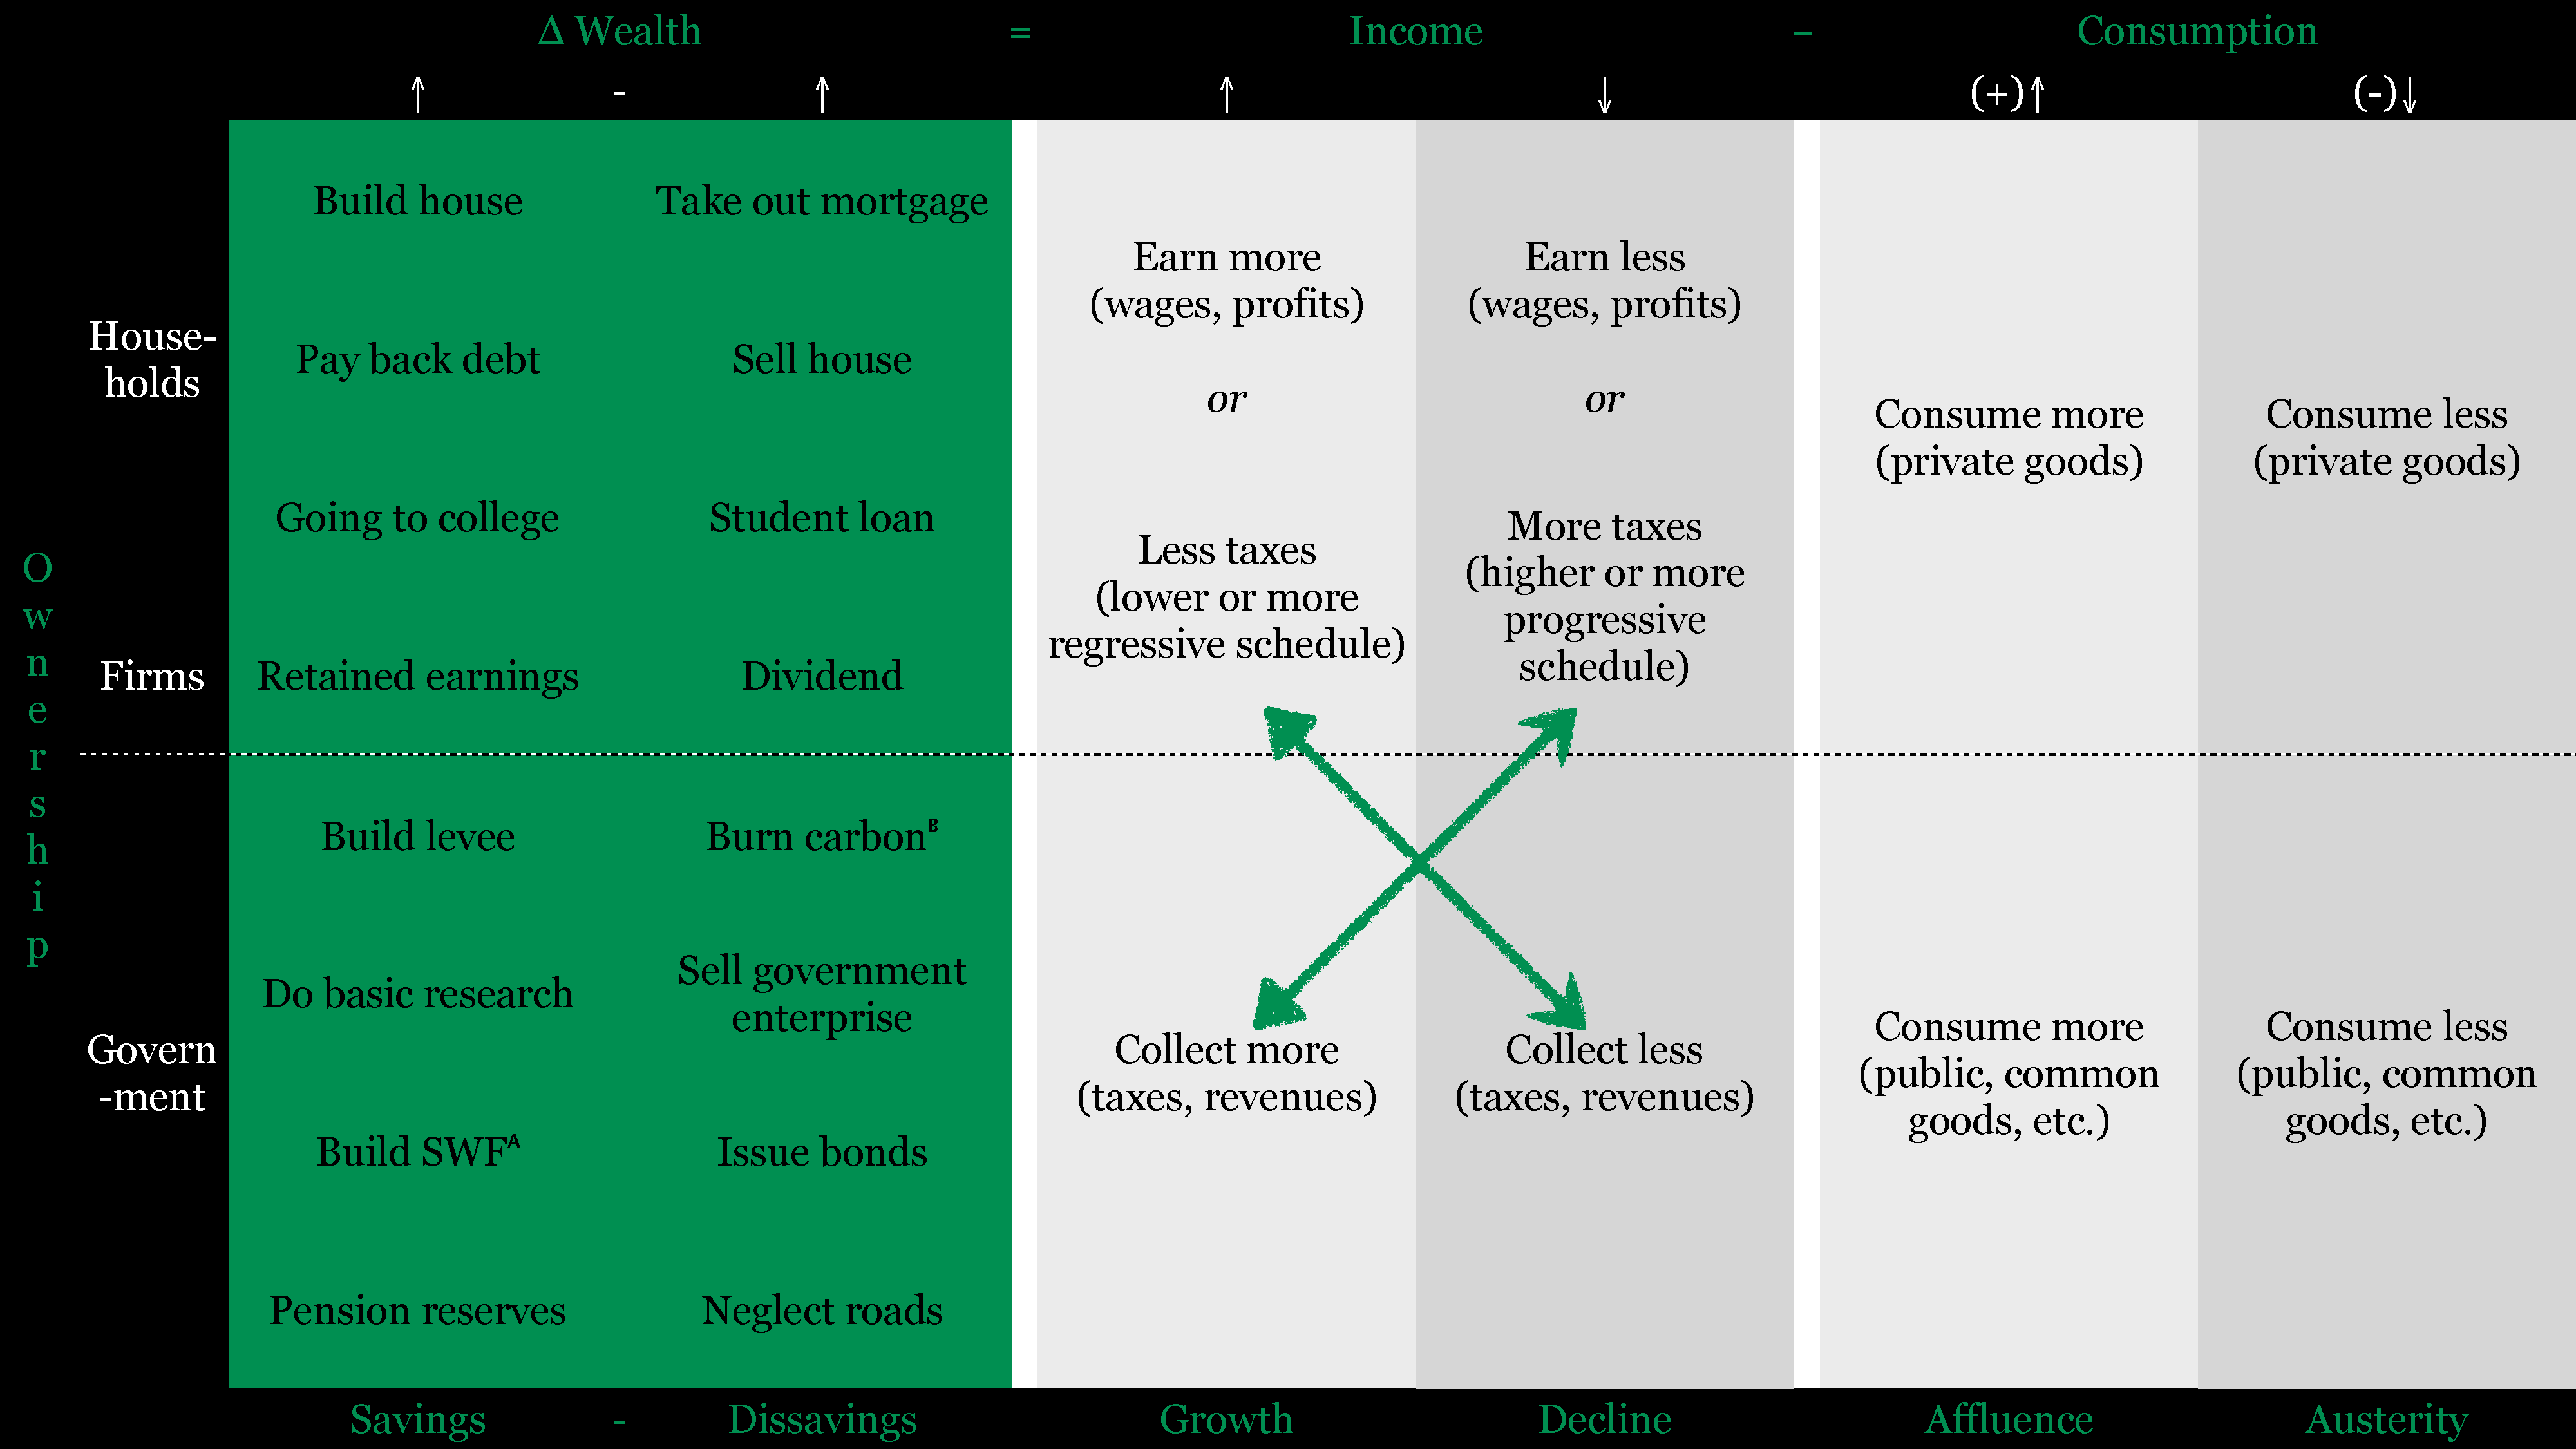
\includegraphics[width=1\linewidth]{haig-simons-individual-collective}
	\caption{Individual and Collective Haig-Simons Identity of Income}
	\label{fig:haig-simons-individual-collective} %again, no green on black please.
\end{figure}

The logic of the Haig-Simons identity, and \autoref{fig:haig-simons-individual-collective} is easy:
you can only have your cake \emph{or} eat it.
Any change in consumption must be matched by a change in income or net worth --- and vice versa.

For instance, a household can afford to build a house either by taking out a mortgage, earning more, or consuming less.

The identity can be balanced \emph{across} households, firms and government, too.
These transfers occur through different financial products and fiscal institutions.
For instance, a household can also afford to build a house if it pays fewer taxes and government accepts less revenue.
Government looses the amount in income that households earn.
\footnote{
	Strictly speaking, this would be the case only for a perfect tax with a zero \gls{DWL}.
}

A comprehensive Haig-Simons identity also includes depreciation (for example, neglected roads) and depleted natural resources (for example, fossil carbohydrates) as real dissavings.
For instance, an economy can consume more than it earns for some time by burning oil.
\footnote{
	Arguably, the past two centuries of growth in the West are to some extent due to the exploitation of fossil fuels.
}
%add source to footnote.
Conversely, a comprehensive Haig-Simons identity also includes real savings such as a newly developed technology or public infrastructure, even when these are not (yet) market priced.
\footnote{
	Preparing a Haig-Simons account on illiquid, public or intangible assets will be difficult.
	As far as possible, accounting should rely on market prices, but will also have to rely on  some planned \gls{CBA}.
}
For instance, an economy can consume less today at equal income and channel the surplus into basic research, \gls{RnD} or send more people to (costly) college.

The Haig-Simons identity of income is a truism similar to the law of conservation of matter.
Surprisingly, it is often ignored or misconstrued, even in \hyperref[sec:Literature]{social-scientific literature} (p.~\pageref{sec:Literature}).
%refer instead here to bastard keynesianism.

I offer two notes to further clarify:
\begin{enumerate}
	\item \emph{Saving $=$ Investment.} In the long run, when industry has adapted and monetary effects have neutralized, all savings are invested.
Saving does \emph{not} depress aggregate demand and choke the economy.

	True Keynesian shortfalls in aggregate demand result from people hording \emph{cash} or equivalents, and not because of an increase in investment.
In deflationary spirals, anticipating lower prices, people cut \emph{both} consumption \emph{and} investment:
the contracted money supply freezes up \emph{all} economic activity.

	This popular conflation of monetary dynamics with savings rates may be one of the most formidable obstacles to enlightened, democratic choice of economic policies and tax in particular.
	\footnote{
		In my ongoing dissertation at \gls{BIGSSS} on the pluralist and deliberative politics of taxation, I call this misunderstanding \emph{Bastard Keynesianism}, gone badly awry.
		I hypothesize that because people do not properly understand the Haig-Simons identity (and the economic cycle), they will erroneously assume that any tax on consumption will hurt the economy.
		In truth, as I argue here, an economy can take on any trade-off between present and future consumption, if only it is phased in slowly enough.

		This confusion, I argue, diverts people away from optimal and fair taxation and effectively curtails the democratic sovereign in pluralism.
	}

	Instead, saving \emph{changes}, but need not depress, aggregate demand;
more capital goods and fewer consumer goods are in demand.
If given enough time, the economy can transform from ``S-classes to school buildings'' without write-downs on unamortized capital investment.
Well-regulated, competitive financial intermediaries will always channel saving into investment.

	An investment is a valuable transformation or improved understanding of our physical world.
It requires labor.
Be it a \gls{SWF} or a savings account, a blast furnace or a green tech patent --- in the final analysis, saving always means to build more things that last longer and/or that we will consume later, instead of things that last a short while and that we consume now.

	Of course, any \emph{one} investment will \emph{ultimately} be consumed or depreciate away.
And we \emph{can} save too much, when capital goods depreciate faster and have such decreased marginal returns that they outstrip our current utility from the same resources (This follows from \cite{Solow1956} theory of growth, p.~\pageref{sec:time}).

	But while that means we should not save endless amounts at any point in time, it does not mean that at some point in time, we should save no more.
There is no economic reason why we could not roll over (limited) savings to our children in perpetuity.

%There is some linke between aggregate demand and inequality, but I forgot which one.

	\item \phantomsection \label{itm:credits-debits-wash} \emph{Dissaving $\neq$ Debt $=$ Deposits $\neq$ Saving.} Dissavings are not the same as debt.
Dissaving is a decrease in net worth of households, firms and economies:
we diminish some durable thing in its value.
Conversely, saving is an increase in net worth:
we add value to some durable thing.

%Deposits is the wrong term, it's savings and when they don't equal investments (that is a Keynesian crisis of low demand.

	In contrast, going into debt does not affect net worth of households, firms or government:
we temporarily gain access to an \emph{already existing} valuable thing (construction man-hours), potentially transform it into something else (a house) and return the valuable thing later (with interest).
Conversely, putting in a deposit (or other credit) also does not affect net worth:
we temporarily grant access to an \emph{already existing} valuable thing to others, for an interest.

	\begin{table}[htbp]
		\caption{Debt and Credit in the Closed Economy}
		\label{tab:Debt-Credit}
		\small
		\begin{center}
		\renewcommand{\arraystretch}{1.5}
		\begin{tabular}{ccc}
			\toprule
			\emph{Households} & \emph{Government}&\\
			\midrule
			$Income - Spending<0$ & $Revenue - Spending<0$&\emph{$\sum$}\\
			private debt & public debt &$=$\\
			(for example, credit card, mortgage) & (for example, government bonds) &\emph{All Debt} \\[20pt]
			$Income-Spending>0$ & $Revenue - Spending>0$ &\emph{$\sum=$}\\
			private credit & public credit &$=$\\
			(for example, deposits, bonds) & (for example, reserves, sovereign wealth) & \emph{All Credit}\\
			\midrule
			& & $\sum=0$ \\
			\bottomrule
		\end{tabular} %double check this table, especially terminology, also consider deposits.
		\end{center}
	\end{table}

	Trivially, public and private debt will always equal public and private credits in the closed economy as summarized in \autoref{tab:Debt-Credit}.
By definition, every debtor needs a creditor.

	Debt and credit define the short-term control of and long-term claims to valuable things and may have distributive consequences, but they do not affect net worth.
Net saving, by definition, does.
\footnote{
	This distinction seems straightforward.
	Yet, similar to bastard Keynesianism, much of public debate of finance and economicsis is marred by great confusion about these basic terms.
	\citealt{McCaffery2005} explains how an inconsistent treatment of debt and capital gains opens up income taxation to ``tax evasion 101''.
}
%make this into another big misunderstanding for my diss?
\end{enumerate}

\section[Smoke \& Mirrors]{Smoke and Mirrors of the Mixed Economy \textsuperscript{\ref{fn:also-in-europe}}} \label{sec:smoke-n-mirrors}

\begin{quote}
	\emph{``If it's too good to be true, it's too good to be true.''}
	\\*
	--- The author's landlady, trained nurse, single mother of three and foreclosed homeowner in Irvine, CA (2007)
\end{quote}

	% \cite{Dwyer2009} 340:
%Indeed, Leicht and Fitzgerald (2006) argue that the middle class has been ‘lent what it should have been paid’ and that a middle-class lifestyle was maintained during a time of stagnant income growth for many at the cost of financial security.

A mixed economy can seemingly overcome its physical limitations and the \hyperref[sec:trade-offs]{trade-offs} (p.~\pageref{sec:trade-offs}) between different ends using a set of smoke and mirrors.

\begin{figure}[htbp]
	\centering
	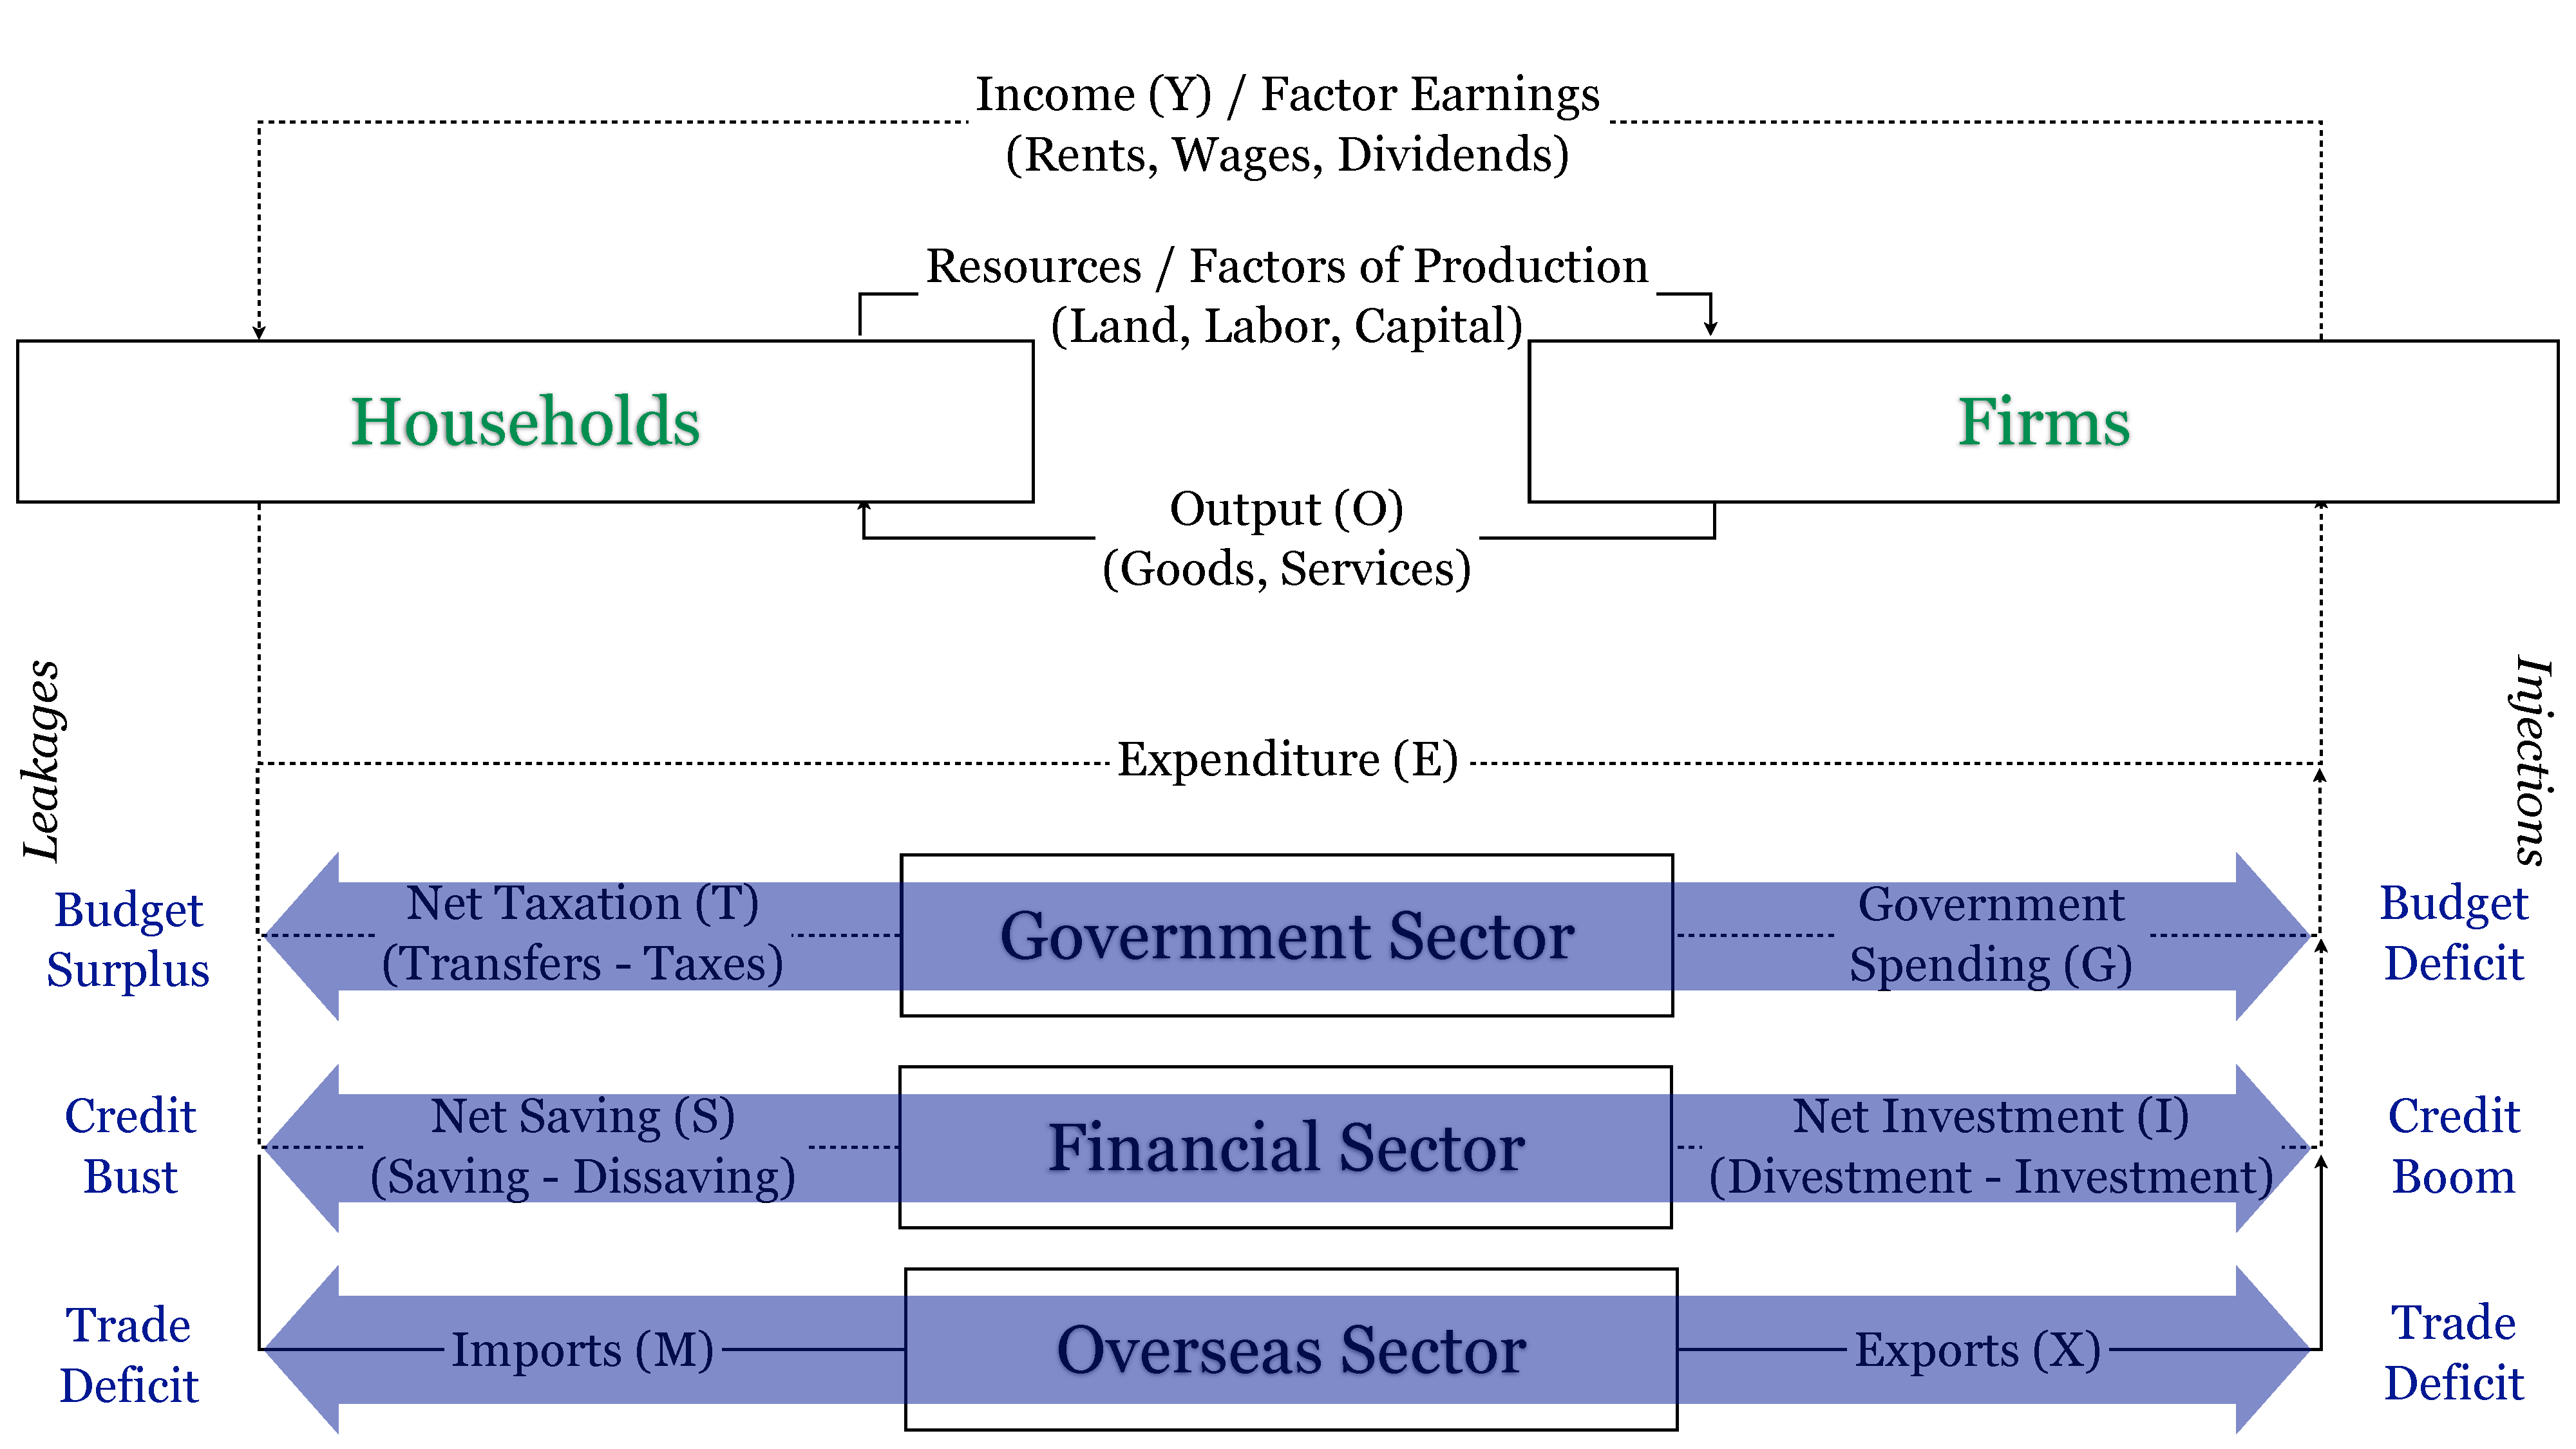
\includegraphics[width=1\textwidth]{circular-flow-with-imbalances.pdf}
	\caption[Circular Flow in the Economy, with Imbalances]{Circular Flow of Income in the Economy, with Macroeconomic Imbalances}
	\begin{flushleft}
		\scriptsize{Compare \autoref{fig:circular-flow-with-imbalances}.}
	\end{flushleft}
	\label{fig:circular-flow-with-imbalances}
\end{figure}
%comment on this!

I briefly explain how three such practices allow us to live beyond our means in the short term:

\begin{enumerate}
	\item \phantomsection \label{itm:credit-bubbles} \emph{Credit Bubbles.} Within the closed economy, \hyperref[itm:credits-debits-wash]{debts and credits are always ``a wash''} (p.~\pageref{itm:credits-debits-wash}).
Still, excessive debt and credit can serve to hide or defer economic trouble ahead.

	In efficient financial markets, credit is extended to households, firms and governments at an interest rate that fully reflects the risk of default.
To assess credit risk, creditors make (and update) predictions about the future solvency (and liquidity) of debtors.

	In the real world, these guesses are sometimes overly optimistic given the available information and credit is extended at too low an interest rate to too many people and organizations.
	\footnote{
		Credit and concomitant asset bubbles can arise for several reasons and according to competing theories, including beauty-contest-type \citep{Keynes1936}, herding \citep{Banerjee-1992-aa} and excessive monetary expansion \citep{Stiglitz2010}.
		An authoritative history of financial crises is \cite{KindlebergerAliber-2005-aa}.
	}
	As long as these risks are not reappraised or do not materialize, an economy can seemingly live beyond its material means.
Eventually, of course, credit bubbles will burst and debtors will partly (have to) renege on their promises to repay interest and principal.
Now, the economy as a whole has to pay for the fat years.

	Credit bubbles are thus always an intertemporal redistribution of wealth from the future to the presence.
	\footnote{
		Conversely, credit crunches, in part, redistribute wealth from presence to the future.
		By keeping the economy below its potential aggregate supply, credit crunches also waste capacity
	}
	When they burst, credit bubbles also jumble ownership rights as defaults spread \citep{Stiglitz2010}.
	\footnote{
		Conventionally, as \citeauthor{Stiglitz2010} points out, a default wipes out shareholders (equity finance) and makes creditors (debt finance) into the new shareholders.
		In the 2007ff financial crises, as elsewhen, economic and political power often intervened to distribute the pain of default differently \citep{Stiglitz2010}.
	}
	Depending on this resulting, quintessential political-economic struggle between debtors and creditors, the brunt of the bursting bubble is allocated between different households, firms and government \citep{Coggan2011}.
	\footnote{
		\citealt{Coggan2011} recently told the history of all hitherto existing society as the struggle between debtors and creditors, to paraphrase \cite{MarxEngels-1848-aa}.
		According to both \citeauthor{Coggan2011} and \cite{Stiglitz2010}, household debtors and governments assumed much of the burden during the 2007ff financial crises, causing, in part, the pursuant sovereign debt crises.
	}
	Similar to inflation and asset bubbles, bursting credit bubbles also redistribute somewhat arbitrarily based on financial product and timing:
people who own equity or leave overheated credit markets early enough, win.
The suckers and laggards loose.

	\item \phantomsection \label{itm:asset-bubbles} \emph{Asset Bubbles.} Concomitant to credit bubbles, bubbles can arise in certain classes of overvalued assets, often including real estate (2007ff), stock (2000f) but also art, oldtimers or essentially useless gold.
Assets are overvalued, when their capital gains are more than what returns can reasonably be expected, given all available information.
%might add piece:
%housing wealth isn't real wealth

	As long as prices do not revert to intrinsic value, people and the economy as a whole can live off the virtual capital gains and beyond its material means.
%explain further:
%they're living of someone else's surplus production, that they have promised to return.

	Asset bubbles, too, redistribute wealth from the future to the presence.
In addition, as pyramid schemes, they redistribute between early investors and later, ``greater fools'' (see \citealt{Stiglitz2010} for a good discussion of the 2007ff crises).

	\item \phantomsection \label{itm:inflationary-pressure} \emph{Inflationary Pressure.} Excessive monetary expansion, aside from fueling credit and asset bubbles can also cause demand-pull inflation.
The onset of inflation and its costs, however, need not be instantaneous.
As upcoming wage-price spirals and increasing inflationary expectations silently add to built-in inflation \citep{Gordon1988}, an economy may enjoy temporarily  heightened output.
	\footnote{
		Traditionally described as an (inward) move along the \cite{Phillips1958} curve.
	}
	As the price level eventually creeps up,
	\footnote{
		An upward shift of the \cite{Phillips1958} curve.
	}
	the economy pays the costs of inflation through depressed growth.

	Grandfathered inflation also redistributes from the future to the presence, and arbitrarily redistributes between cash-denominated and other ownership claims, between debtors and creditors.
	\footnote{
		In addition, the costs of later disinflation may be large.
		Prescriptions for disinflation and expected costs differ.
		%add literature quotes.
	}
\end{enumerate}

\paragraph[Too Good To Be True]{Too Good to be True.}
In summary, an economy cannot produce and consume above its long-run growth path of outward shifting aggregate supply.

Trivially, the wealth of an economy is determined by its natural resources, technology, human and physical capital --- all \emph{tangible things}.
When these capacities are fully utilized (as they are \emph{not} in a cyclical downturn or debt-deflation crisis), no financial or monetary charlatanism can take us beyond them in the short term.
Any short-term gain that a bubble or excessive monetary expansion will bring only defers the day of this reckoning.

\section[Real Dissavings]{Real Dissavings of the Mixed Economy} \label{sec:real-dissavings}

\begin{quote}
	\emph{``When the last tree is cut, the last river poisoned, and the last fish dead, we will discover that we can't eat money.''}
	\\*
	--- Greenpeace
	%horrible quote
\end{quote}

\begin{quote}
	\emph{``Give me chastity and continence, but not yet.''}
	\\*
	--- \citeauthor{St.AugusteofHippo397} Confessions (VIII, 7)
\end{quote}

Our economies substantially dissave in ways that are not reflected in conventional macroeconomic data.
These \emph{real} dissavings, or ``off-budget fiscal activities'' \cite[49]{Bonker2006} include population aging,
\footnote{
	The second demographic transition (\citealt{Davis1945}, restated by \citealt{Caldwell-1976-aa}) delivered low, often below-replacement level \gls{TFR}.
}
depleted natural resources (land, oil, water), exhausted common goods (global warming
\footnote{
	The greatest, widest-ranging market failure in the history of mankind, according to \cite{Stern-2006-aa}.
}
) or failed public goods (immunization?), to name just a few.

These processes all unambiguously degrade something of economic value, and should be recorded as consumption in our aggregate Haig-Simons accounts (as I have suggested in \autoref{fig:haig-simons-individual-collective}, p.~\pageref{fig:haig-simons-individual-collective}).
%wuppental institute has some accounting data on this.
%%is this the right fig label?

%ode to the mixed economy old ending is missing.
%\subparagraph{Property is Power} This argument points to the fact, that from an equity perspective, not only consumption of resources is consequential, but also excessive ownership.
%Great wealth, in this view, bestows great power on owners when they make supposedly discretionary (rather than fully rational) decisions in investing their capital.
%
%To some extent, this justification rests on the assumption that owners of great wealth do indeed make discretionary investment decisions.
%
%\subparagraph{Broad Ownership is Great for Incentivizing Work} Particularly in situations where asymmetric information on work performance abounds, sufficient wealth is required to make workers stakeholders in an effort to overcome incentive problems \marginpar{\textsf{(Cite game theoretic literature here, ask Professor GrÜner for more stuff.)}}.
%Asymmetric information on work performance is frequently the case in the non-routine or non-manual work characteristic of post-industrial production \marginpar{\textsf{(cite literature here on post-industrial production, maybe \cite{Bell-1973-aa})}}.
%
%\subparagraph{Counteracting Runaway Capital Accumulation} The scale-free dynamic of increasingly networked post-industrial society suggests that rewards may be increasingly non-Gaussian in their distribution (``Extremistan'' in \cite{Taleb2007}'s pop-scientific terms) \marginpar{\textsf{(cite \cite{Taleb2007} here extensively, but also \cite{Kleinberg-2009-oz} and others on network theory)}}.
%If these assumptions are, in fact, correct, wealth distribution may become increasingly fat-tailed, with a self-perpetuating dynamic of runaway capital accumulation in the hands of few.
%That could --- leaving aside the aforementioned equity concerns --- possibly disrupt a meaningful link between effort, risks and rewards.
%A PAT would then be justified to counteract these potential dynamics.
%
%\subparagraph{How to Implement It}
%First of all, organizing capital redistribution through taxing assets, not incomes, has some merits in itself.
%It does not, like the progressive income tax, tax saving twice and create disincentives for investment.
%If anything, this ``expropriation'' tax should encourage risk-taking and investment, much like low central bank interest rates do \marginpar{\textsf{(na, did I get this right?)}}.
%
%A PAT, however, carries a number of risks and uncertainties.
%First of all, when some of its revenues end up being consumed, it reduces the overall savings rate of an economy, which is detrimental to future growth \marginpar{\textsf{(Cite optimal or sustained growth literature here, also demographic change.)}}.
%
%Similarly, a PAT will reduce the collateral of big investors which can depress the business cycle.
%It will be necessary to implement a PAT during a boom and administer it in carefully anticyclical fashion (high taxes during boom times, low taxes during busts).
%
%To avoid these downsides of reduced aggregate saving and collateral, a PAT should be implemented as a merely redistributive instrument --- from one ``owner'' of an investment, to another ``owner'' but never to consumption.
%The other owner could be both the state, or individuals.
%The PAT could, potentially, change not only the spread but also the kind of investment, boosting state-directed public/common-good natured investment, such as education.
%Policy makers may find it helpful to exclude PAT revenues from the calculations of public deficit limits.
%
%\paragraph{3) \href{http://maxheld.de/2009/10/26/progressive-consumption-tax/}{Progressive Consumption Tax}} The (postpaid) progressive consumption tax (PCT) is the one lever both to extract revenues and also to redistribute consumption checks.
%It taxes consumption at a progressive rate, thereby resolving the dilemma of neutral, but regressive indirect taxation and progressive, but distorting, direct taxation \citep{McCaffery2005}.
%
%The PCT leaves all incentives and prices intact with the exception of the one thing it intends to tax:
%excessive, wasteful, conspicuous consumption of positional, Veblen goods \marginpar{\textsf{(Cite Veblen here.
%Ok, I may have put a little too many adjectives in this sentence.
%It's a draft, after all)}}.
%
%The PCT is no harder to administer than the progressive income tax.
%It taxes that part of last year's net worth, plus this year's incomes which is not at the bank (or stockbroker) at the end of this year, and thus consumed.
%Losses from investment are credited as negative incomes, just like capital gains.
%Both are not taxed.
%Loans or payments on principal and interest, both of which do not change net worth, are not included as incomes or losses, but are taxed, when consumed.
%Durable goods as well as real estate, both on the borderline of consumption and investment, are taxed according to depreciation schedules.
%
%\textsf{(Note to self:
%still need to address and understand the issue of goods with extremely low depreciation, or even appreciation of positional goods, such as diamonds and high-end real estate.
%What do do about them?
%Use asset tax for that purpose?
%Use an effective rental utility for the consumption tax?
%- I think McCaffery has written about this)}.
%
%\paragraph{As Close to a Beer Coaster Tax as it Gets} This set of taxes does away with the need for any further redistributive taxes.
%In particular, there is no more need for the always ``messy'' corporate income tax.
%Under progressive asset and consumption taxation, there is no possibility to forestall incomes in corporations.
%
%\subsubsection{Why They're Great}
%(Insert here a section on why the above tax structure is great, make it systematic according to some criteria.
%Preliminary ideas:
%\begin{enumerate}
%	\item{Progressive}
%	\item{Elegant, Simple}
%	\item{Minimal Distortion of the Market}
%	\item{No Disincentives for Work, Risk-Taking}
%	\item{No Uniform Progression-Mess, Tax-Evasion}
%	\item{Pro-Cyclical?}
%	\item{Factor Specificity:
%Which Factor is Burdened?}
%\end{enumerate}
%
%This is also where the application of Rawslian ``reflective equilibrium'' takes place:
%a pragmatic-spirited going back-and-forth between normative ideas and what is reasonably conceivable given \cite{Rawls-1971}.
%
%\subsubsection{Focus on Consumption}
%
%Of the above-mentioned three taxes, one is chosen in particular for further elaboration as a normative hypothetical to the current political economy:
%the progressive consumption tax.
%
%It is the most interesting tax for a number of reasons.
%First of all, it has never been implemented, and hardly ever attempted (with the exception of the Unlimited Savings Allowance Bill in the U.S.\ Senate in xxxx \marginpar{\textsf{(insert citation, details, here)})}.
%Secondly, it is the most innovative, and arguably, positively disruptive tax.
%Thirdly, it is what could be called, a somewhat post-ideological proposal for tax reform:
%it does not easily fall on (and then, down) one either side of traditional left-right divides.
%It curtails excessive consumption, but leaves incomes and assets untouched.
%
%For the analytical purposes of establishing a normative hypothetical to the currently existing international political economy, the PCT may not be the most straightforward proposal --- rather, the asset tax comes to mind.
%The PCT, like all other the other three taxes suggested here, \emph{does} in fact require a full degree of international tax harmonization and cooperation in the OECD-world:
%without full accounting of incomes, irrespective of their origin, the PCT is doomed to fail.
%A possibly resulting outflow of consumption to other countries under tax competition would be a further problem\footnote{The Negative Income Tax, by virtue of its affecting a relatively immobile base, could initially be thought to be relatively independent of international tax competition.
%It however requires a massive revenue base to finance the colossal redistribution it entails, and thereby rests on an internationally harmonized tax regime.}.
%
%To formalize the suggestion:
%Independent Variable:
%International cooperation (levels:
%autonomy, competition, cooperation)
%Dependent Variable:
%Efficiency and Equity, in the long run
	\chapter[Three Crises]{A Tale of Three Crises}
		\label{chap:3-crises}
		%!TEX root=../tax-democracy-held.tex

%Some kind of introduction, what are those bumps?
%they are interlinked

%overall quote

\chapter[Three Crises]{A Tale of Three Crises} \label{chap:3-crises}

%the headings in the below stink

\section{The Crisis of the Welfare State}

\begin{quote}
	\emph{``Private affluence, public squalor.''}\\*
	--- John K. \citealt{Galbraith1959}
\end{quote}

%cite some Butterwegge work on inequality
%cite some Groh-Samberg work on inequality

	%Baumol explicitly endorses tax hikes to make sure that cost disease doesn't cause public squalor \cite{Baumol1992}
	
	%note that much of the economics in here are what is known as "comparative statics"

\subsection{Excessive Inefficiency is Inequitable} \label{sec:InefficiencyIsInequitable}
Equity and efficiency, at the extremes, are not as conceptually orthogonal as conveniently assumed: Excessive inefficiency is, in fact, likely to be inequitable, too, as government failure to provide public goods and pool risks has a social gradient. Poorer individuals will be hit harder, because public goods and lemons markets are not, in truth, dichotomous and uniform phenomena. In the real world, some public goods (for example, policing) have close, if costly private good substitutes (for example, gated community). Similarly, some risks will be more symmetrically observable (for example, buyers of private health insurance in Germany tend to be better and better-known risks). Alternatively, rich people may have enough assets to forego risk pooling alltogether (for example, excessive co-payments). In short, rich people can often buy their way out of otherwise underfunded or failing public institutions, creating yet greater inequities \citep{Barry2002}.

%Moreover, inequality and common/public goods and risk pooling are not as distinct concepts as presented in the above table, when taken to the (reasonable) extreme and adding a dynamic dimension. 
%
%Inequality is, in the above assumed to be a policy challenge in its own right, that calls for \emph{redistribution}. Alternatively, from a more dynamic perspective, gross, self-reinforcing inequities could also be framed as public or common good problems, where excessive inequality exerts a negative externality of non-opportunity on the poor. Taking things further into the future, presently existing inequality could be assumed to exert a negative externality on the future, forgoing otherwise more broadly-based growth.
%
%Conversely, excessive underprovision of common/public goods or a lack of effective risk-pooling easily hits the poor hardest, who have few other resources to buy or substitute the lacking goods.
%
%Policy makers should, however, be careful not to introduce duplicate redistributive mechanisms in other state activities, such as Pigouvian taxes or fees, which are not geared towards everyone, but a certain type of behavior or service consumed. 
%
%A further requirement of ``regulatory neatness'' and corrolarly of this thinking is that redistributive and revenue-generation taxes should in principal be levied on natural persons exclusively. Only between natural persons is redistribution meaningful, even ignoring the above-mentioned problems of incidence and uniform progression discussed in the above. 

\subsection{Excessive Inequality is Inefficient}
\label{sec:InequalityIsInefficient}
Equity and efficiency are not a zero-sum trade-off. Sometimes, when the cake is sliced up more equitably, it may grow. Formulations of such positive-sum relationship between the two vary, and only some examples can be given here.

%also cite here the Jacobs mathematician \cite{Lorenz2013} et al who seem to have done some kind of portfolio modeling to show the same thing. this is about human capital. get into this. this might belong somewhere else.

%note (this is from somewhere, either Cassidy or Frank, probably frank, that more equality can make more Coase-style deals happen; that's what you want, be it in Coase-style property rights or Pigovian taxation. You don't want: having distributive stuff kreep into commons et al. Good example: Pendlerpauschale in Deutschland. This is an important point, I think this also works with only the harms principle as justification. Don't let go off this point.
	%Argue: It's always better to have coase-theorem style exchanges on common goods rather than to regulate them (also: exernalities), examples including airplane tickets when they're overbooked, it's no longer first-come-first-serve, but you get a compensation for volunteering (auctioned off). %idea from robert frank on the dawin economy. Re-read ch 6 on the coast theorem and in paying for public goods.
	%The thought is this, beginning in chapter 8: if there's income economy inequality the demand for public goods is likely to decrease, because willingness to pay differs greatly between different users of the public good. Example: public goods costs 1000$, equal use for 2 people, but b/c of very different incomes, their willingness to pay is 900 and 200, and so it's not happening maybe.
	%This is interesting, because, here's a Caplan-Style political economy (all cost benefit), and even THIS is plagued by income inequality. If you have lesser income inequality, this decision even in a caplan world would work.

\subsubsection{Structural Unemployment} \label{sec:StructuralUnemployment}
%instead of structural unemployment speak of natural unemployment, which is frictional PLUS strucltural (unions, min. wages, efficiency wages/aka reserve army). Opposed to this is cyclical unemployment

Extreme inequality in post-tax market outcomes may also conflict with the efficiency goal of full factor employment. Most (post)industrial societies have legislated socially accepted minimal incomes. This legislation takes the form of statutory minimum wages or unemployment benefits. Either way, an effective or de-facto price floor for wages is established\footnote{Income subsidies or negative income taxes may not lead to such dysfunctional price floors (\hyperref[http://maxheld.de/2010/04/19/sharing-the-burden/]{c.f.} \citealt{Held2010}).}. People with productivities \emph{below} this price floor will not find employment, leading to a DWL of structural unemployment\footnote{I assume here that market wages are low \emph{only} because of low productivities, in keeping with \hyperref[sec:PerfectCompetition]{perfect competition} condition {itm:PriceTakers} (\hyperref[itm:PriceTakers]{infinite buyers and sellers}). If, by contrast, employers have great bargaining power over non-unionized workers (as appears to be the case in much of the service sector) they may receive low wages even when their labor productivities are adequate. Such Manchester-capitalism styled exploitation should be met with regulatory, not fiscal interventions: otherwise, government may end up transferring to exploitative firms.

It does not matter \emph{why} labor productivity of some groups of workers is in \emph{relative} decline. Candidate culprits include international trade and finance (for example, discredited \citealt{Stolper1941}) as well as skill-based technological progress \citep{Card2001}. Whatever the reason for low relative labor productivities, an efficient fiscal configuration should help factor markets clear.}.

Crucially, the level of minimal incomes depends on the broader configuration of tax incidence, indirect taxes in particular. When taxes are relatively flat and fall on labor or consumption, the real costs of living for low-income earners rise. This \emph{tax wedge} can take the form of (flat or proportional, payroll-style) social contributions, VAT or a relatively flat or proportional personal income tax: either way, \emph{more} money has to be made on the market for the same living standard (in Purchasing Power Parities, PPP).

The implications for tax design are twofold:

\paragraph{Structural Unemployment as Endogenous.} 
The only genuine fix to structural unemployment is of course more education to lift people, or at least their children, out of their low standards of productivity. Better education, to be sure, will require fresh ideas --- but also lots of public resources. Well-funded public education, in turn, is endogenous to a fiscal configuration (compare \autoref{sec:Underqualification} on the \hyperref[sec:Underqualification]{real dissaving of underqualification}).

\paragraph{Structural Unemployment as Exogenous.} 
Even from a static perspective, assuming low-productivity workers to be exogenous, some measure of tax relief for would-be working poor may enhance welfare. An efficient tax system should reduce the burden on low-productivity earners, to keep their post-tax socially acceptable minimum wages as low as possible. 
\newpage
\begin{desideratum}[Low Cost of Living for Low-Productivity Earners]
	A desirable tax has a minimal incidence on low-productivity earners to lower their cost of living.
	\label{des:low-price-floor}
\end{desideratum}

\subsubsection{Excessive Inequality Squanders Talent.} 
Extravagant inequalities that bear no meaningful relationship between effort and reward squander talent as Malcolm \citeauthor{Gladwell} argues in \emph{Outliers} (\citeyear{Gladwell}). This pop-sociological debunking of the meritocratic myth resonates with needs 
	%style!
for a large and highly qualified workforce, and concerns of social immobility in (post)industrial economies (for example, Lisbon Strategy, EU 2020). For a knowledge economy, you need lots of qualified and motivated people, not just a few stars.

\subsection[Heterogeneity]{Heterogeneity: The Sources of Wealth} \label{sec:sources-of-wealth} The \gls{EU} is a union of very unequal member states. On of the richer large member state, France (\$ 44,747 nominal \gls{GDP} per capita according to the IMF 2010) is six times richer than the poorest member state, Bulgaria (\$ 6,334 nominal \gls{GDP} per capita, \emph{ibid.}.). Within \gls{EU}-15, Luxembourg's \gls{GDP} per capita in \gls{PPP} was 3,5 that of Portugal. Within \gls{EU}-27, that multiple has widened to 7,4 times Luxembourg and Bulgaria (\citealt{Alber2008}: 1). %add gini, other union level statistic?

%capital formation is a better term than accumulation

Why this difference?

\paragraph{Productivity} The wealth of nations, as Adam \cite{Smith-1776-lq} taught, ultimately depends on labor productivity. Both nations and people prosper when they can get much out of the ultimately scarcest resource, human effort. 

This labor productivity, as \gls{GDP} per capita, varies widely between rich (for example, France 116) and poor (for example, Bulgaria 41.3, both in 2010, indexed to EU-25 average, Eurostat 2010)\footnote{
	Current labor productivities, as \gls{GDP} per capita probably understate the discreptancies. They are both after (much) regional integration. Without trade and investment --- ex-ante EU membership --- domestic economic output might be much lower still.}. 
Labor productivity, in turn, depends on technology (\gls{TFP} or Solow residuals), human capital (skills) and stocks of physical capital (for example, factories). These achievements, tangible or not, are all past surplus production coagulated into some form of capital. At some point in the past, someone had to have an extra bit of time or food on her hands to build something lasting, above and beyond subsistence consumption.
	%TFPs and Solow Residuals are important!

%financial intermediaries are: banks, funds, insurance. They do different jobs. For financial paper: these products and intermediaries are great, they do great things.


Why does it matter?

\begin{enumerate}
	\item Because capital is transformed surplus production, it is always an inheritance from the past. And so, much of current output depends on past capital accumulation and its historical circumstance in geography, geology, culture and political institutions. It matters a great deal, which circumstances encourage saving and innovation, but that question need not concern us here. %add link saving

	However, we need to remember here, that current performance is \emph{not} sufficiently linked to current output. Romanian workers at Dacia, a car manufacturer, produce less value in an hour primarily \emph{not} because they are lazier or sloppier, but because Romania lags in capital accumulation and cannot provide them with the skills and machinery that their French counterparts at Renault have. 

	\item Because capital is transformed surplus production, differences in output between people, countries and regions are here to stay, at least for some time.
\end{enumerate}

%more stats are here: http://epp.eurostat.ec.europa.eu/tgm/table.do?tab=table&init=1&plugin=1&language=en&pcode=tsieb030, 

I now discuss some broad economic dynamics likely operating on this partially integrated, and enormously heterogeneous economy. 

%money is: medium of exchange, unit of account and store of value. It can be either commodity money (intrinsic value), or it can be fiat (paper, paypal, bitcoins). The money stock is very difficult to know because the definitions are vague.

%The result of the two crises is an economy with runaway inequities, foregone productive capacity and a suboptimal net savings rate, in the face of greater challenges ahead (for example, aging, global warming).

%First, developed welfare states, in spite of their unprecedented prosperity, appear to be increasingly constrained in their ability to raise revenue and redistribute it as their legislators see fit. 

%Structural underfunding is caused by a state that is increasingly unable to raise sufficient revenue necessary for the provision of risk pools, public and common goods, as well as to finance its allocative goals.

%The result of the two crises is an economy with runaway inequities, foregone productive capacity and a suboptimal net savings rate, in the face of greater challenges ahead (for example, aging, global warming).

 \begin{figure}[htbp]
	\centering
	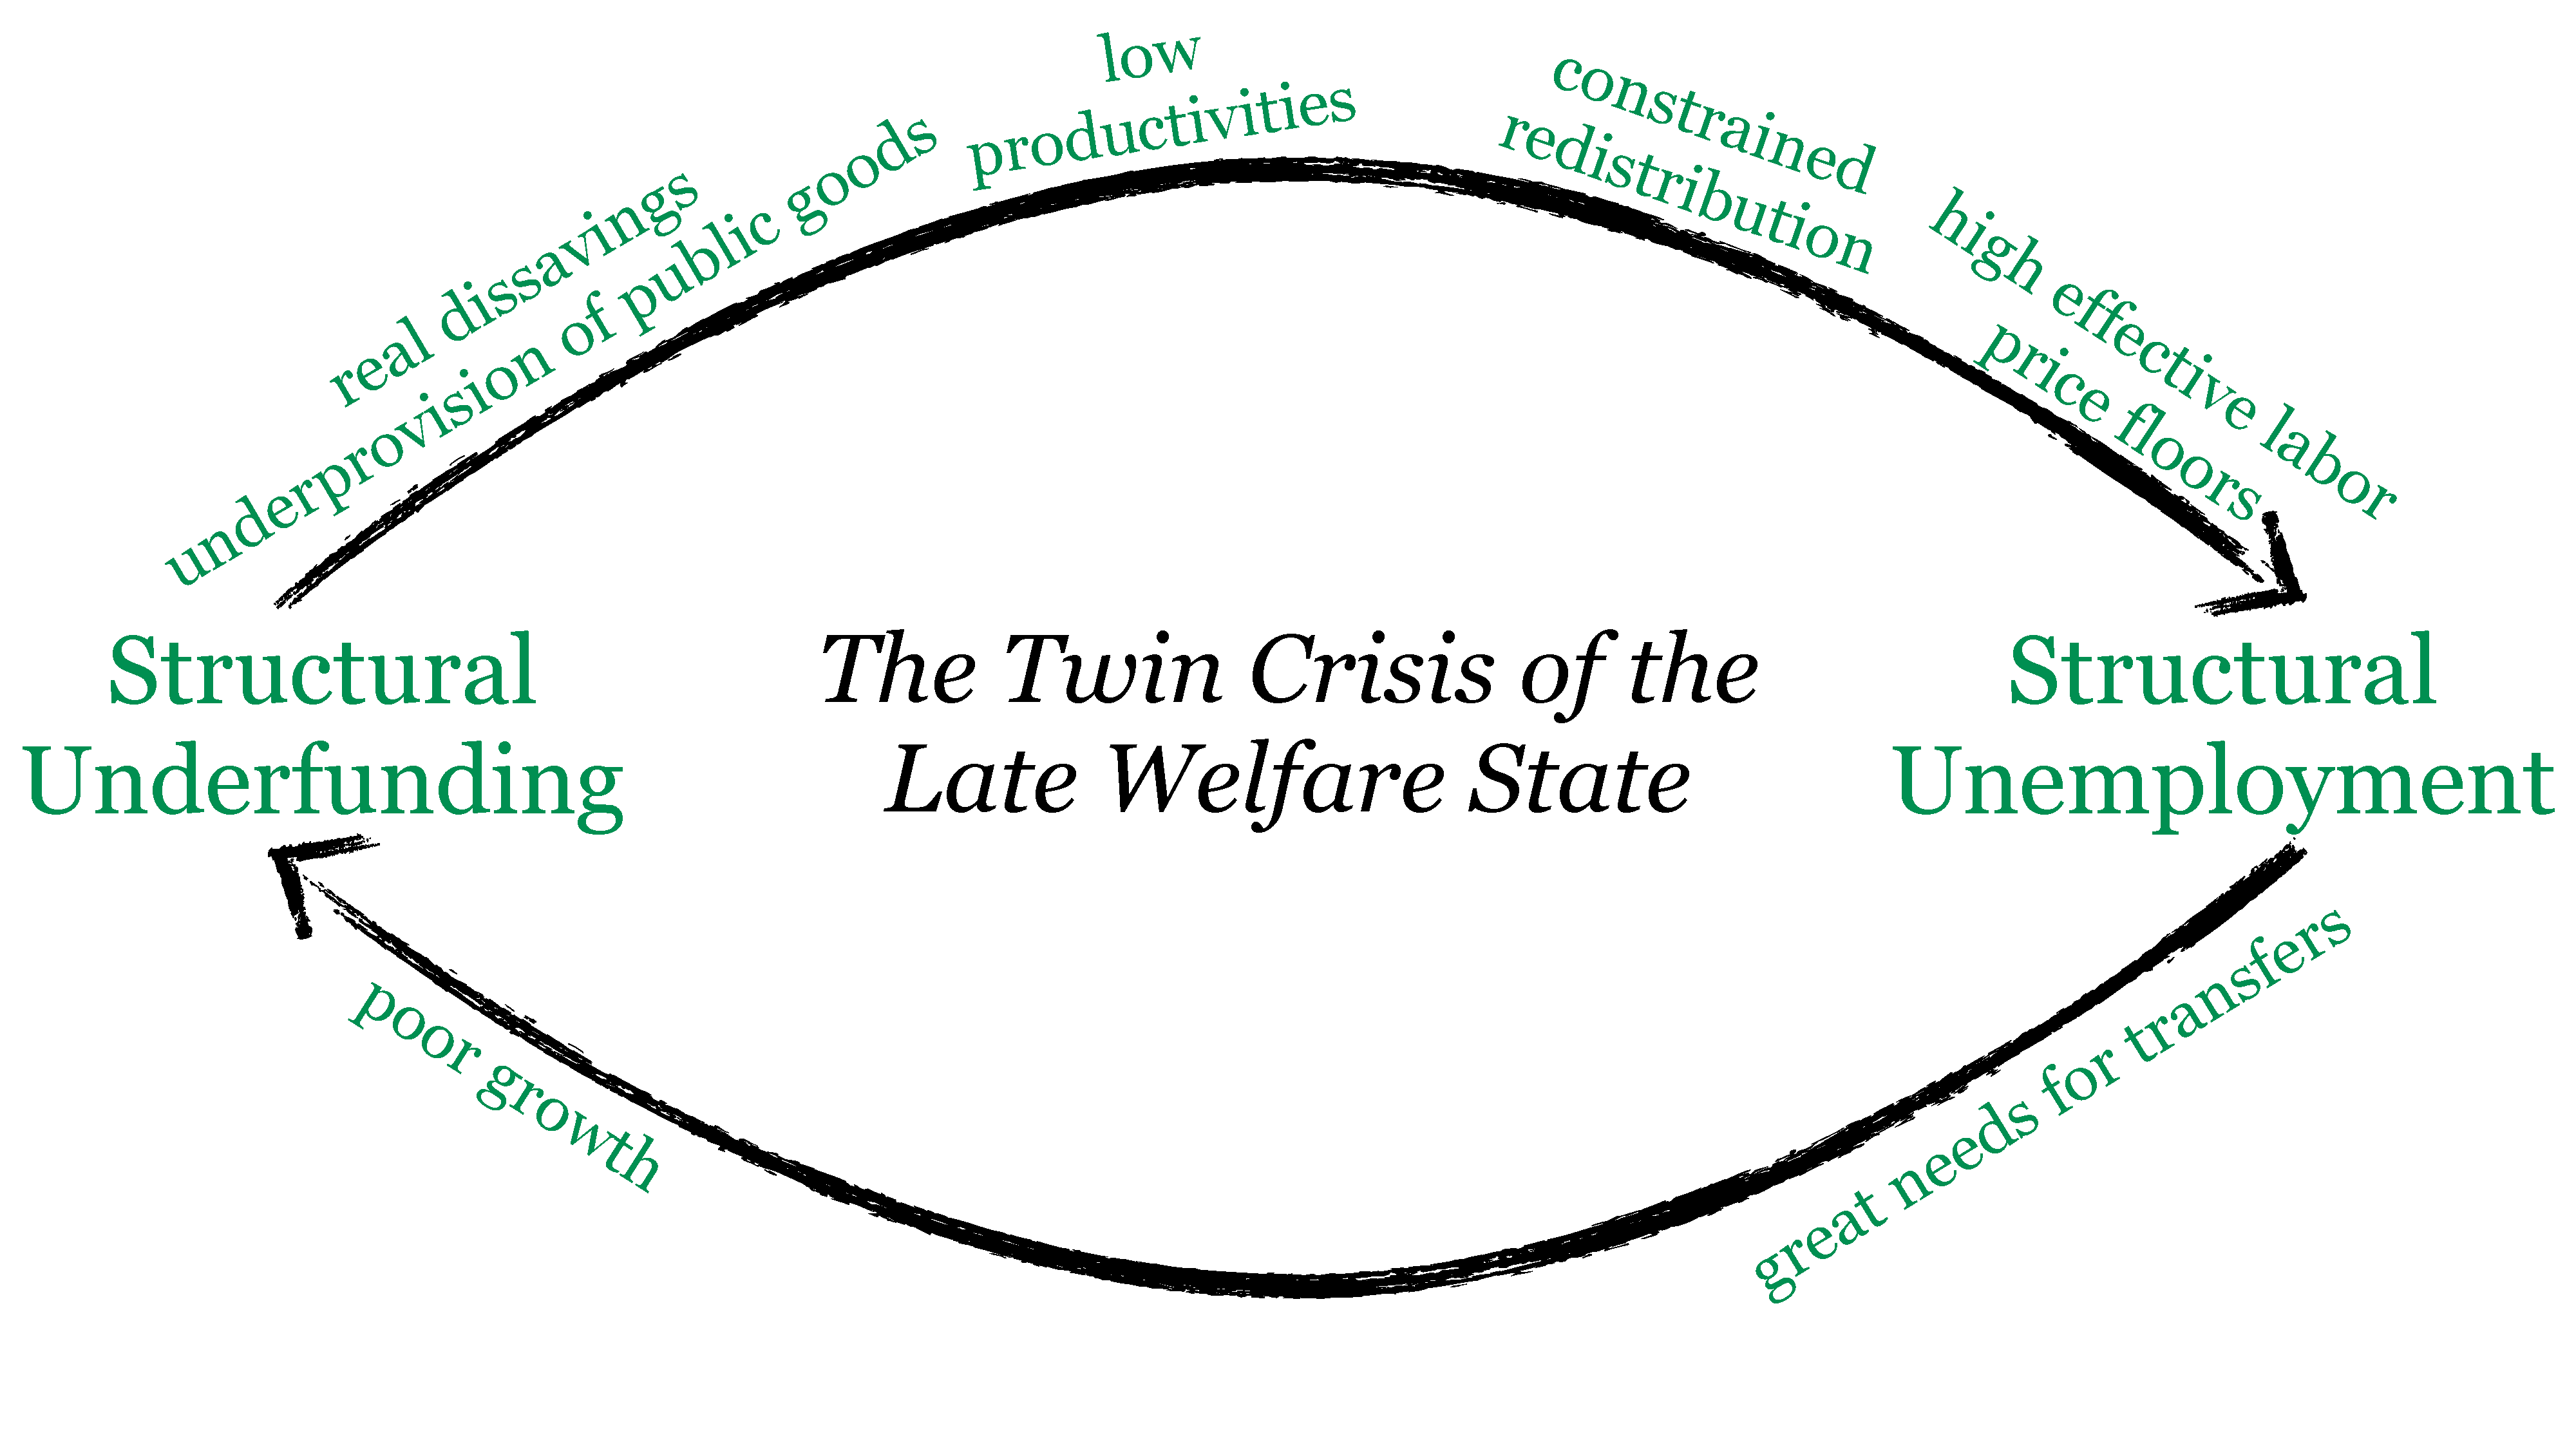
\includegraphics[width=1\linewidth]{dual-crisis}  
	\caption{The Dual Crisis of the Late Welfare State}
	\label{fig:dual-crisis}
\end{figure} 

%Today, welfare states are challenged or changed on a number of fronts. Internally, welfare provision is challenged by aging societies in the developed world, with resulting higher dependency rates and costs under “pay-as-you-go” systems (Castles 2002). Moreover, revenues and costs are affected by prolonged and extensive macroeconomic disequilibria, especially structural unemployment (which of course, can also be an effect of inadequate welfare regime design). Decreasing rates of productivity and output growth have heightened concerns, and de-industrialization and increasing flexibility of working arrangements have called existing setups into question, especially those featuring corporatist institutions.

%Add Twin crisis picture here

%The result of the two crises is an economy with runaway inequities, foregone productive capacity and a suboptimal net savings rate, in the face of greater challenges ahead (for example, aging, global warming).

\section{The Crisis of Democracy}

\begin{quote}
	\emph{``%We had to struggle with the old enemies of peace: business and financial monopoly, speculation, reckless banking, class antagonism, sectionalism, war profiteering.
	They had begun to consider the Government of the United States as a mere appendage to their own affairs. We know now that Government by organized money is just as dangerous as Government by organized mob. Never before in all our history have these forces been so united against one candidate as they stand today. They are unanimous in their hate for me --- and I welcome their hatred.''}\\*
	--- Franklin D. Roosevelt (Washington, DC, 1936)
\end{quote}

%other quote: that is why i get a little discouraged sometimes ...

%Blog post
	%Fortschritt ist, wenn wir etwas (1) gemeinsam Beschlossenes, Vernünftiges und Gutes erreichen, (2) dass uns freier und gleicher macht, (3) auch gegen Widerstände. Wir müssen uns also zusammenraufen und der Sphinx sagen, welche Antwort sie für uns alle einloggen soll, damit Fortschritt passieren kann. Seit 225 Jahren machen We the People das mit Abstimmungen und Freiheitsrechten. In unseren pluralistischen Demokratien kämpfen Interessengruppen um die politische Macht im Staat. Bürgerinnen verfolgen diesen Wettkampf in der Zeitung, schließen sich, folgend ihren gegebenen Interessen Gruppen zusammen, wählen die ihnen am nähesten stehende Partei — und das ist dann das gute Ende der Geschichte. Oder?

	%Auch auf dem deutschen und europäischen Marktplatz der Ideen sind Dumping-Anbieter unterwegs. Unser Politik-Ramsch kreischt nicht schrill, er lullt uns ein in seiner ganzen, miefigen Mittelmäßigkeit: konzeptionell, rhetorisch, visionär. Wir tauschen keine Argumente aus, denn Basta, es gibt keine Alternative. Wir nennen keine Gründe, denn wir nehmen ja “Augenmaß“, “machen unsere Hausaufgaben” und halten unsere “Hände ruhig“. Was bedeuten diese betäubend-sinnentlehrten Phrasen?
	
	%Amerika und uns plagt die gleiche Krankheit, in unserem gemäßigten politischen System schreitet sie nur schleichender voran. Es ist eine schlimme Krankheit, bei der sich der demokratische Prozess loslöst von den tatsächlichen Abstraktionen, die unsere Welt regieren und den machbaren Alternativen, die sich unserem Gemeinwesen bieten. Entscheidungen werden bestenfalls im Hinterzimmer verkuhhandelt, meistenfalls gewinnt der Status Quo und schlimmstenfalls diktieren wenige Interessierte. Wir raufen uns nicht mehr zusammen, wir raufen nur noch zusammen.
	
	%Früher war nicht alles besser, aber manches einfacher. Wenn in den 50er Jahren ein Kumpel für mehr Mitbestimmung die SPD und ein Beamtin für bessere Pensionen die CDU wählten, dann lagen sie damit beide grob richtig, folgten ihren gegebenen Interessen.  Wenn 2013 eine Häuslebauerin gegen Eurobonds die CDU und eine Bandarbeiterin für paritätische Sozialabgaben die SPD wählt, dann ist das nicht mehr so klar (vielleicht deshalb und deshalb). (Glücklicherweise) funktioniert unsere Demokratie nicht mehr als Zuschauersport, in dem wir einfach jeder alle vier Jahre das für sich bessere Team wählt. Von den billigen Plätzen ist es einfach verdammt schwer geworden zu sehen, wo das Tor steht. Die weiter hinten sitzen können nur hoffen, dass die Trainer es sehen, die Wahrheit sagen, und das Spiel nicht längst gekauft ist.
	
	%Ich will nicht Politikerinnen verunglimpfen oder Wählerinnen verhöhnen. Sie tun, wir alle tun das im gegebenen Rahmen Mögliche. Nicht alle Politikerinnen sind schlecht oder alle Wählerinnen dumm, sondern die Institutionen der pluralistischen Demokratie überkommen. Die Komplexität und Ungerechtigkeit unserer Welt passt nicht in eine SPON-Fotostrecke, nicht in 1:30 Tagesschau. Unser Gemeinwesen braucht keine harte aber faire Arena, sondern die Sendung mit der Maus.

%what might be wrong with current democracy?

%check the quotes, comments in: \cite{Bluhdorn-2007-aa}

%check the quotes, comments in: \cite{Crouch2004}

%Second, my research interest emerges from a sense of utter disconnect between political debate and the abstractions and interests governing the political economy. This dis-connect is evident in misleading sloganeering (‘Mehr Netto vom Brutto’, more net out of gross income), widespread superstitions (‘employers [sic!] pay half of social insurance’), bastard Keynesianism (‘consumption is good!’) or redistributive smoke grenades (‘we should tax companies’). At a deeper level, I wonder whether pluralist interest and electoral re-presentation can still be reasonably assumed to yield efficient and equitable policies, in an ever more complex world marred by cooperation problems.

\subsection{Crisis of Micropolitics}
%People are cognitive misers (Kahneman + Tversky 1983)

\subsection{Crisis of Macropolitics}

%Ryfe 2005
	% note in my discussion of the crisis of democrac that in the US the associations that used to do much of the helpful aggregation (and maybe deliberation) have withered, cf putnam 2000
	%Cite this guys for the logic why a random sample is better.
	
\subsection{Crisis of Policies}

\subsection{Supply and Demand}
%don't hate the players, hate the game.

%\section{Why is campaign spending on the rise? --- \\The empirical dynamic}

		%\subsection{Broader dynamics of political competition: Dealignment \& Individualization}
	%To understand why campaign spending is on the rise, we need to look at the broader and changing dynamics of political competition. Change in political competition is of course ambiguous and multi-faceted. Two powerful themes emerge from much of the literature, which will help to contextualize rising campaign spending: dealignment and individualized targeting of voters.

	%\paragraph{Dealignment}
	%When \citet{Lazarsfeld1968} went out to Erie County, OH in 1940 to figure out ``How the Voter Makes up His Mind in a Presidential Campaign'' they found that citizens voted in relatively socio-economically homogenous groups, that socio-economic status neatly predicted their voting behavior. Also, people would typically vote as their parents had, and swing- or late-deciding voters where relatively scarce.

	%This has since changed dramatically. Party alignment as weaked, arguably both as a corellate of a broader disaffection with (mass) associations \citep{Putnam-1995-aa} as well as as a function of an unfolding value space, whose multiple dimensions two (or even multi-) party systems can no longer accomodate \citep{InglehartWelzel-2005-aa}. 

	%\paragraph{Individualization, Targeting of Voters}
	%The second, not entirely disjunct trend is one of individualization \citep{Beck-2002-aa}. The lifestyle choices of people diversify, and become (at least superficially) more independent from socio-economic status. 

	%This sociological trend is part and parcel with the emergence of new means of production, that allow for customization of products and services. 

	%Also, advances in information technology allow for an ever greater degree of automatic capture and intelligent analyses of these increasing differences between people. In the ream of political campaigning, this is happening in targeted political advertising. 

	%As \citet{Malchow2003} describes in his handbook of political campaigning, modern technologies in analysis (ranging from the mundane correlation and regression to cutting-edge neural network modeling or data-mining) and information-\emph{narrow}casting (for example: from ZIP-code cable TV to bloc-specific mailings, or household-specific phone banking) allow professional campaigners to act on the increasing differentiation of lifestyles. Specifically, Malchow advocates that professional campaigners use as much available (seemingly unrelated) lifestyle and otherwise information to concentrate their efforts on those voters they are most likely to activate (for GOTV efforts), convince (for swing voters) or persuade (for supporters of the opposing party).

	%\paragraph{Political Campaigning under Dealignment, Individualization}
	%What does money spent in campaigns have to do with all of this? Simple: the above trends of party dealignment and individualization, in the current configuration of political competition \footnote{More on the arguably dysfunctional dynamic of the current configuration of political competition in my other assignment}, require intensive professionalization of campaign efforts (otherwise referred to as ``Americanized'' or post-modern campaigns), which in turn, is costly. 

	%Once this dynamic is set in motion, as \citet{Gibson2001} argue, typically by electoral defeats, followed by changes in internal leadership and a consolidation of power at the center, other competing parties have to follow suit. \citet{Strachan} observes this dynamic even at the grassroots-level of local campaigns, where alternative, low-budget, face-to-face campaigning was the norm until recently: ``Jack didn't want to do the kinds of things candidates have to do. It's commendable to run a race on \$50,000, but when the opponent has \$400,000 he sets the rules, and that's what happened in this race''  (\citealt{Strachan}: 72).

	%Professionalization, and with that, increasing spending of political campaigns, then emerges as a dominant strategy, speaking in terms of game theory: no matter what the other party does, you're always better off professionalizing. And low-budget campaign ``collusion'', while potentially Pareto and socially optimal (as is arguably the case at the municipal level), becomes a Prisoner's Dilemma of cooperation.

	%\section{How does increasing campaign spending affect the political process? --- \\The normative debate}

	%\paragraph{The Facts: Money Doesn't Seem to Buy Elections}
	%Conventional, if cynical, wisdom holds that with increasing spending, money can buy elections. Empirical findings supporting that claim, however, are scarce. In a cleverly designed study, comparing repeat contestants (thereby controlling for a large share of candidate-inherent qualities) in U.S. House elections, \emph{rogue economist} \citet{Levitt1994} found no significant effect of campaign spending on electoral outcomes, controlling for a large number of other factors\footnote{Levitt, concerned with social welfare, however, concludes from this finding, that some cap on campaign spending would be beneficial, as results are unlikely to change and wasteful, irrational extravagance could be avoided.}.

	%An intuition along these lines, doubting the measurable effectiveness of one's campaign and spending was also offered by Frank Stauss of the Berlin-based Butter agency in class, reflecting on the impact of the 2009 SPD federal campaign.

	%\paragraph{The Path-Dependency of Professional, Expensive Campaigns ---\\ Leading to \emph{Hyper-Majoritarian} Democracy?}
	%A methodological note of caution should be in order here. Levitt's, as much of the other research on the impact of campaign spending (and its antecedent professionalization) was based on majoritarian systems \citep{Lijphart-1999-aa} of governance in the Anglo-American world. With their single-member plurality electoral system (``First Past the Post'', FPTP), and its correlate two-party system, it appears reasonable to assume that most electoral contests would feature only two (reasonably feasible) candidates, who will relatively easily achieve some degree of media and otherwise exposure in their districts. Under proportional representation electoral systems (PR), where more parties compete not just for plurality seats, but for percentages of the popular vote, ex-ante exposure of candidates may be much more unequally distributed, with many of them marginalized.

	%As Levitt implicitly concedes in his paper, fundraising is likely subject to great path dependencies and economies of scale: it is disproportionately easier to raise funds for a successful, well-known candidate than for other, less well-known contestants. Even in systems where all, or more of campaign spending is publicly funded (as in many European systems), a similar dynamic is conceivable. Also there, public funds depend on past performance at the polls, and, if campaign spending is to feature curvilinear effects, path dependencies could be at work.

	%Taken together, the possibility of hyper-majoritarian competition in both consensus as well as majoritarian democracies arises, where few candidates (or issues, or parties) stand a chance at gaining some popular support, given how high the ``market entry costs'' are. Granted, however, the recent German trend for large parties to loose shares seems not to support such a dynamic.

	%\paragraph{The Ties That a \$1000 Breakfast Plate Binds ...}
	%More questions towards the legitimacy of high campaign spending, and, related, private fundraising remain. Even if Levitt is right as it seems, and private campaign donations are unable to buy elections, it is conceivable that, given the Prisoner's Dilemma of high-spending, donors may be able to exert undue influence on or at the least, access to office-holders.

	%\section{Conclusion}

	%I first conclude that private campaign donations should be outlawed, if only for the reason of \emph{suspected} undue influence. In all of the below, I refer to a scenario of high, but entirely publicly funded campaign expenditure.

	%\paragraph{Campaign Spending and Trends in Representative Democracy:\\ Yes, It Is Inevitable}
	%I conclude from the above, and the potential Prisoner's Dilemma-type competition between parties, as well as the broader trends of dealignment and individualization, to which professional, expensive campaigns respond, that indeed, higher campaign spendings are an inevitable outcome for all representative democracies.

	%\paragraph{Campaign Spending and Voter Apathy}
	%Going back to the aforementioned background trends and correllates of high campaign spending, party dealignment, and individualized targeting, given persistent if not increasing voter apathy I wonder whether really, the link with high campaign spending is a causal one.

	%It could well be argued that voter apathy, possibly caused by dealignment and a misconfiguration of the political competition, is the independent variable to which frantic individualization and expensive professionalization of campaigns are merely dependent responses.

	%But more importantly, I wonder whether increased campaign spending is not completely epiphenomenal to the potentially misaligned political competition, and related voter apathy. At least at the federal or state level, it appears inevitable that cheap, unmediated, face-to-face campaigning for representative democracy, is no option. As simple and reliable class voting patterns dealign and dissolve, previously instrumental to mass mobilization, more (financial) effort to communicate competing ideas is clearly necessary.

	%Much rather, it seems possible that the slicing and dicing of the electorate into neatly defined groups, some (or many) responding strongly to their own (if relatively irrelevant or ill-defined) ``hot-button issues'' will lead to a political competition at the lowest, dysfunctional denominator. I try to explore how such a dynamic could work in the other assignment.

	%I would then conclude that high campaign spending is not as such the problem for voter engagement, at least if realistic opportunities for entry are available to new contestants or ideas. With a publicly funded, regressive schedule of campaign finance (relatively less money for successful parties in the past, a sort of party ``infant-industry'' protection), and political competition about the \emph{true} alternatives (not ``issues'') of public policy, effectively communicated and exchanged, expensive campaigns should be considered a wise investment, not a frivolous extravagance.


%The crisis is not one of overload, that i expect Crozier, Huntington and Watanuki (1975) as cited in Warren 2003, but one of underresourcing. And in these questions you always have to think about the ideal, utopian hypothetical, which, sadly, we hardly ever do.

%=== Make-up piece for roemmele class

%\begin{quote}
%	\emph{We are not as divided as our politics suggest.}\\\\
%	Barack H. Obama in his keynote speech at the 2004 DNC convention
%\end{quote}

%\section{Democracy: What are the Rules of the Game?}
%How do we compete on that marketplace of ideas, that democracy seeks to provide? How do we, as voters, decide where to cast our ballot? How, and about what, do parties communicate to their voters? And how is all of that aggregated into seats in parliament, and into majority governments?

%These questions are as old as mankind's first attempt at Athenian democracy, c.a. 400 BC. Answers vary widely, from the liberal and representative, to the communitarian and direct forms of democracy.

%Today, representative democracy, based on the ideas of liberalism and enlightenment, is the norm. It's perseverance notwithstanding, recent innovations in the field of information and communication technology and a wide-reaching trend for professionalization of political campaigns, warrant a re-assessment of the empirical reality and theoretical axioms of liberal, representative democracy.

%In the following, I synthesize past empirical and theoretical works on the topic, and hypothesize how professionalized campaigns, given largely de-aligned and irrational voters, could lead to a dysfunctional political competition.

%\section{How it Used to / \emph{was Supposed} to Work...}

%\subsection{Preference Aggregation in Liberal, Representative Democracy}
%Liberal, representative democracy, rests on a pluralist theory of governance (\citealt{Louw2005}:15). Pluralism, being both empirical hypothesis and normative prescription supposes that political power is, and \emph{should} be widely dispersed among society's interest groups. These interest groups, made up of ever active citizens, openly compete with one another, thereby preventing any one of them to become a dominant elite.

%Institutional manifestations of pluralism abound in today's real existing democracies, both of the majoritarian and consociational type \citep{Lijphart-1999-aa}, including the right to form parties, (particularistic) associations, minority protection as well as constitutional checks-and-balances on government.

%\subsection{An Economic Theory of Democracy}
%Anthony \cite{Downs-1957-aa}, in his seminal spatial modeling of democratic competition, expanded pluralism into a democratic theory of public choice, based on the rational self-interest of both voters (to live under policies they prefer) and politicians or parties (seeking or maintaining political power).
%\begin{figure}
%	\includegraphics[width=1\columnwidth]{Downs-Median-Voter}
%\label{fig:Downs-Median-Voter}
%\caption{The Median Voter (Downs 1957: 118)}
%\end{figure}

%\paragraph{The Median Voter}In its simplest form, reproduced in \autoref{fig:Downs-Median-Voter}, the ``Economic Theory of Democracy'' suggests that in a unimodal, unidimensional and symmetric distribution of voter preferences under a single-member plurality (SMP) electoral system, only two parties will compete for the median voter, taking on a central position only marginally different from one another. Any new parties or otherwise diversions from the median position would quickly move towards that equilibrium position again.

%Downs provides a theory, explaining how differing preferences and disjunct interest groups get channeled into fewer parties and stable equilibrium.

%\paragraph{The Median Voter\emph{s}}In Downs' defense from often misconceived reiterations and undue criticism: his theory, misleadingly reduced to a ``Median Voter Theorem'' does \emph{not} stop here. He employs his theory to a wide range of given preference distributions and electoral systems, including multimodal distributions (with \emph{several}, local median voters), multiparty competition under proportional representation and antecedent coalition government. He even suggests, in a prelude to the much later ``issue'' literature (for instance \citealt{Abbe2003}), that parties may choose to ``sprinkle'' their position over a number of issues, so as to appeal to a broader electorate (\citealt{Downs-1957-aa}: 137).

%\paragraph{In a Nutshell ...} What remains of Downs' theory, and is of central importance here is distilled in the following axioms:
%\begin{enumerate}
%	\item{Voter preferences can be modelled on a \emph{single dimension}.}
%	\item{Voter preferences are \emph{presocial}, or given \emph{ex-ante}.}
%	\item{The mode of party competition is a function of the voter preference distribution and the electoral system.}
%	\item{In the equilibrium, any mode of the preference distribution is occupied by a party, so as long as the electoral system threshold allows for another party.}
%\end{enumerate}

%\subsection{The Good Old Days: Late-Modern Pluralist Political Competition}
%Both \cite{Lazarsfeld1968} study of the 1940 U.S. presidential campaign and \cite{LipsetRokkan-1967-aa} historical account of party systems and voter alignments serve well as a contrasting foil for the post-pluralist critique to come.

%\paragraph{Erie County, OH, c.a. 1940}Let's begin with Lazarsfeld, who in 1940 set out to study how voters made up their mind in Erie County, OH. He found a highly stable, neatly aligned political spectrum. 77\% of the voters, he found, voted as their parents and grandparents had (\emph{ibid.}: xxxiii). People thought politically, as they were, socially: ``social characteristics determine political preference'' (\emph{ibid.}: 27) in that long past rural county. Also, and most significantly for the criticism to come, Lazarsfeld found that:
%\begin{quote} \emph{A very large majority of \textbf{both} groups thought that it would be the common man, the plain people, the working class, who would benefit if Roosevelt were elected. \textbf{Both} groups also agreed, although not to the same extent, that Willkie's victory would be best for the business class.\\ (\citealt{Lazarsfeld1968}: 28, emphasis added).} 
%\end{quote}
%Where campaigns where influential, they acted to make voting \emph{more} consistent with the social group of the voters (\emph{ibid.}: 139).

%This is of course a finding very much in line with the modeling assumption of \cite{Downs-1957-aa}: voter preferences seemed to differ on a single dimension, and, to a large extent, where given.

%\paragraph{Where You Stand on an Issue Depends on Where You Sit ...}
%\cite{LipsetRokkan-1967-aa} provide a broader history of social cleavages and and antecedent voter alignments and party systems, of which the ``worker'' --``business'' nexus in Erie County is only the last of a number of stages. Analyzing the history of political competition in Europe, they lay out a dialectic of conflict and integration, ranging from early modern centre-periphery and church-state struggles to early-industrial urban-rural and late-industrial owner-worker conflict (\emph{ibid.}: 93). These evolving cleavages, in their account, shape and diversify preferences and parties as new ones layer on past ones, slowly fading away. While their historical analysis is limited to Europe, a broader insight remains: how, at least in the past, political preferences and parties followed broader patterns of socio-economic difference and bifurcation\footnote{It should be noted that \cite{LipsetRokkan-1967-aa} with their suggestion of layered, cross-cutting cleavages, do of course stand in sharp contrast with \cite{Downs-1957-aa} assumption of a unidimensional preferences space. The implications of this early, conceptual disagreement with Downs are however of little relevance to the argument presented here.}.

%\paragraph{No Nostalgia...}
%To be clear, not all was good in Erie County, OH, c.a. 1940. These neatly-aligned voters, following more their family tradition than their own thinking, were far away from to the ideal of a well-informed, active citizen. The socio-economic determination of the preferences they displayed are the vert politics of zero-sum redistribution, which all too often result in violent strife and the destruction of a democratic system. This bifurcated electorate is the very antithesis to those cross-cutting cleavages that at least the consociational theorists of democracy cherish so much \citep{Lijphart-1999-ab}.

%\paragraph{... and yet: it \emph{Worked}}
%Its non-emancipated voters and explosive configuration notwithstanding, some key characteristics of this late modern political competition seem worthy do condense, building on the aforementioned axioms of Downs:
%\begin{enumerate}
%	\item{Political preferences are presocial, given ex-ante.}
%	\item{Political preferences are determined by socio-economic status.}
%	\item{Political parties compete on differential policies, geared to different socio-economic strata, but on the same dimension.}
%\end{enumerate}

%\section{A Doubtful Demand Side: The Woes of the Rational Voter}

%\subsection{Our Dumb Voters: Non-Attitudes}
%The first grain of normative and conceptual doubt in the reliability of a Downsian, pluralist aggregation machine comes from \citeauthor{Converse-1970-aa}'s \citeyear{Converse-1970-aa} seminal work on ``Attitudes and Non-Attitudes''. In his panel studies, he finds that a substantial sub-group of voters has entirely random attitudes on, amongst others, the relative role of government and the market, with close to zero correlations between test and retest. This result, Converse warns, holds even when respondents were encouraged \emph{not} to respond. Moreover, the subgroup that displays random attitudes is more likely to report extreme attitudes in either direction.

%Less elegantly modeled, but more broadly applied findings come from a vast array of public opinion surveys, aptly summarized by \cite{Delli-CarpiniKeeter-1996-aa}. Findings suggest that many voters do not have even the most basic knowledge of political processes or platforms. 

%A discussion of the complications and questions that arise from this area of research is beyond the scope if this treatment, and with limited relevance to the question at hand. 

%It remains to be noted that the Downsian \citeyearpar{Downs-1957-aa} assumption of pre-social, unidimensional preferences, and to an even greater extent, Lazarfeld's \citeyearpar{Lazarsfeld1968} findings of socio-economically determined preferences, may no longer apply given widespread ignorance of voters. 

%More generally, these findings cast doubt on the liberal assumption that an \emph{electoral} democracy with pre-social preferences and particularistic interest representation will achieve socially optimal decisions.

%\subsection{\emph{Rational Ignorance} to the Rescue}
%Theorists of Rational Choice respond to these doubts by pointing out that ignorance may well be rational, given how small a chance an individual vote stands to turn the election (particularly under SMP) \citep{Olson-1971-aa}, and that largely ignorant masses can still produce socially optimal outcomes if their errors are random \citep{Page1993, Surowiecki2004}. 

%While I find the pride, that evangelists of Rational Choice take in the Olsonian escape from participation quite dubious, a broader appraisal of the merits and problems of Rational Choice is beyond the scope of this piece. 

%It will suffice to accept their framework of human motivation and to simply question the empirical validity of the ``Wisdom of Crowds''. This argument presented by a host of authors (see above), and recently popularized by \cite{Surowiecki2004} proceeds as follows: if all those ignorant voters cancel each other out in their \emph{random} aberations from the socially optimal, the remaining, knowledgeable voters will decide the election, as \emph{their} choices will differ \emph{systematically} from the mean.

%\subsection{What if Errors are Systematic?}
%Bryan \cite{Caplan2007} has recently provided ample evidence and a compelling framework to cast doubt on this assumption. In his passionate dismantling of ``The Myth of the Rational Voter'', he describes how uneducated opinions on economic matters will \emph{systematically} differ from the average, following what he describes as an \emph{antimarket}, \emph{antiforeign}, \emph{make-work} and \emph{pessimistic} bias.

%If \citeauthor{Caplan2007} is right, and voters do in fact err systematically on matters which they understand inadequately, there will be no Wisdom of the Crowds, but instead a tyranny of the biased masses.

%\subsection{What if the Value Space is \emph{N}-Dimensional?}
%Another set of empirical finding incompatible with \cite{Downs-1957-aa} assumption comes from political sociology, where an entire field of sophisticated surveys and competing theories has evolved, probing into the dimensionality and change of the postindustrial value space. 

%It will suffice to point to one set of findings here. In their work, \cite{InglehartWelzel-2005-aa} not only single-handedly integrate value change into a reanimated version of modernization theory, they also provide a host of empirical findings from the World Values Surveys, showing that, at the least, the value space is now two-dimensional, with an axis of traditional vs. secular-rational values, and a second axis of survival vs. self-expression values. The authors describe a wide-reaching change in direction, from the former pre-modern to modern dimension to the latter modern to postmodern dimension, but note that this is neither an irreversible nor universal process and that in any given society, people will differ on more than one dimension. Other, broadly corroborating findings come from \cite{FlanaganLee-2003-aa}, who explicitly relates value change to a complication in political competition and \cite{Schwartz-1994-ab}, who suggests a whole circle\footnote{The problem of visualizing more than two dimensions in a \emph{circle} is duly noted. From statistical work for Chris Welzel, this author can attest to the apparent necessity to (overly) simplify empirical findings of the value space until they are readily presentable in two-dimensional form. Such multidimensional scaling and forced factor analyses at almost all cost in terms of model fit, to the author, indeed appears to be a troubling habit of value research.} of independent dimensions.

%\subsection{Problems with Downs}
%From these empirical findings and conceptual refinements arise a number of potential incompatibilities with Downs model of political competition and antecedent, optimistic ideas of socially optimal public choice under pluralist democracy:
%\begin{enumerate}
%	\item{A substantial subset of voters appears to harbor irrational, and systematically skewed beliefs. A simple aggregation of preferences appears unlikely to result in socially optimal policies.}
%	\item{Any given postindustrial electorate is likely to differ on more than one dimension in their political preferences.}
%\end{enumerate}

%These incompatibilities alone, albeit preliminary in nature, would require a thorough rethinking of pluralist prescriptions and analyses of liberal, representative democracy undergoing Downsian aggregation.

%\section{Messing with the Supply Side of Democracy ---\\A Theory of Dysfunctional Political Competition for Dealigned and Irrational Voters}

%\begin{quote}
%	\emph{I'm a little angry that I apparently was voting in a completely different election than most of the country. I thought we were having a rational discussion about how best to protect ourselves in perilous times ---\\ and actually, it was a referendum on boys kissing.}\\\\
%	Comedian Bill Maher on his HBO special ``I'm Swiss'', referring to the 2004 U.S. presidential election.
%\end{quote}

%Speaking in economic terms, the preceding section dealt with questions regarding the \emph{demand side} of \citeauthor{Downs-1957-aa}'s \citeyear{Downs-1957-aa} ``Economic Theory of Democracy'': the condition and abilities of voters.

%In the following, I want to direct the view to the \emph{supply side} of political competition: to the parties and candidates that compete for majorities and to the campaigns they wage. 

%\subsection{A Neo-Downsian Theory of Dysfunctional Political Competition}

%To hypothesize a Neo-Downsian Theory of Dysfunctional Political Competition, accounting for and problematizing the above described dynamics in political campaigning, I add to \cite{Downs-1957-aa} model specification the following:
%\begin{enumerate}
%	\item{Voters differ in their preferences on a number of mutually orthogonal dimensions.}
%	\item{Voters differ in the importance they assign to different dimensions.}
%	\item{Voters differ in the importance they assign to positions \emph{along} one dimension.}
%	\item{Parties can choose which dimension(s) to campaign on. No agreement on dimensions is necessary.}
%	\item{Campaigning is costly.}
%	\item{Costs are the financial and otherwise efforts required to activate or convince a voter of any party given position on any given dimension.}
%	\item{Dimensions have different cost functions.}
%	\item{Cost functions are allowed to take any form, independent from the preference distribution, and including skewed and/or multimodal. (See \autoref{fig:Neodowns})}
%	\item{Parties aim to maximize their utility function, where marginal costs of campaigning are same as marginal vote increases.}
%\end{enumerate}

%\begin{figure}
%	\includegraphics[width=1\columnwidth]{NeoDowns}
%\label{fig:Neodowns}
%\caption{The Median Voter (Downs 1957: 118), with an inverse cost function overlaid. For more intuitive appeal, the overlaid function is \emph{not} the cost function, but the propensity of voters at the given position to be activated or convinced by a campaign.}
%\end{figure}

%It is unfortunately beyond my abilities to completely visualize the multidimensional model specified in the above, which would also have to be fully specified in formal math for further elaboration.

%For illustration, I have merely overlaid a hypothetical cost functions to Downs classic graph in \autoref{fig:Neodowns}. 

%\paragraph{Introducing Variable Costs of Campaigning} It is first assumed that voters do in fact, vary in their preferences on more than one dimension. The number of, and potential correlations between dimensions (making them less than completely orthogonal in a multidimensional scaling) is of no concern here. Furthermore, the costs and rewards of campaigning are overlaid on Downs model.  It is assumed that the effort required to activate (GOTV) or convince a voter vary as a function of her position on the chosen dimension. It is furthermore assumed that these cost functions differ in their overall integral as well as their shape: some dimensions are cheaper to campaign on overall, and some positions on some dimensions are easier to communicate than others.

%The above model specifications also allow voter preferences to vary in importance \emph{across} different and \emph{along} single dimensions. It is assumed here that these differences in assigned importance of voters are fully captured in the cost functions of the parties. This is a reasonable simplification: voters will be more easily (and cheaply) activated on positions and/or dimensions they already feel strongly about.

%\paragraph{How Will Parties Act} The incentives for parties to act are then substantially complicated. They will no longer, as \cite{Downs-1957-aa} assumed, simply compete for a vote share around some mode in the unidimensional preference distribution. Instead, given their budget constraint, they will choose their positions on, and dimensions they compete on, as a function of their campaigning costs and the chances to activate or convince a voter. In simple terms: they will campaign so as to maximize the ballot bang for their buck.

%From these incentives then emerges a rationale to choose positions \emph{between} preference distribution modes (the classical Median Voter prescription) and nereby, \emph{local} minima in the cost of campaigning function, or conversely, \emph{local} maxima of importance assigned by voters.

%Parties will multiply the ex-ante preference distribution with the costs of campaigning function and solve for that position that offers the best ratio of votes for campaign money invested. Exogenous budget constraints of parties may further alter this calculation.

%\paragraph{Introducing Strategic interaction}
%Choosing party platforms, and campaign positions is of course, as \cite{Downs-1957-aa} pointed out, a \emph{strategic interaction}, or simply: a game. The rationale of one party to choose a position depends, amongst other things, on the chosen positions and dimensions of all competing parties.

%This further complicates party incentives. As parties in an election --- per definition --- care about \emph{relative} payoffs, rather than \emph{absolute} payoffs, they will choose positions and dimensions, which, based on the real or anticipated campaigning of competing parties, will offer them the relatively highest ballot bang for the available campaign buck.

%\subsection{Different Dimensions for Different Voters}
%\paragraph{Converse, Redux: A Sweet Spot for Dumb Voters?}
%This model becomes more tangible and persuasive when interpreted in light of \citeauthor{Converse-1970-aa}'s \citeyearpar{Converse-1970-aa} insights. His subset of ``random'' voters appears to be more likely to be easily swayed by campaigns on dimensions \emph{different} from the mainstream of political competition than those ``systematic'' voters who held reliable, and potentially educated beliefs on the relative role of government and the market. 

%Without conceptually stretching Converse's finding too far, they can at minimum be interpreted as support for the model's specification that different groups of people can relate with different ease and reliability to different dimensions. In political campaigning, that ease and reliability translates into campaign spending required to harvest voters.

%Converse's staple item on the relative roles of government and the market, appears to be a suitable dimension to appeal to some, educated voters who will \emph{systematically} respond to positions taken by competing parties. Other voters, who have displayed \emph{randomly} changing attitudes on the subject matter are unlikely to be reliably activated or persuaded by campaigns on this dimension. For them, in particular, other dimensions unbeknownst to Converse may be more suitable.

%Note also that the second, uneducated group of voters may be \emph{per se} more interesting to political campaigns: with relatively less developed political attitudes, and party alignment they constitute a battle ground where potentially, with the right, effective dimensions chosen, many more votes are at stake for political campaigns. By contrast, the group of educated voters with systematic and stable responses on the government-market dimension may be hard to win over, and relatively ineffective to mobilize given the typically higher turnout among these voters. 

%In the language of the proposed model, the first, uneducated groups may provide a number of dimensions on which cost functions have a relatively small integral, or provide concentrated, ``sweet spots'' where a large number of voters can be reached with little effort. Put provocatively, dumb voters may just provide parties with more bang for the buck.

%\paragraph{False Class Consciousness, Redux: Screwing \emph{Joe the Plumber}}\footnote{No pun intended.}

%\begin{quote}
%	\emph{It's not surprising then they get bitter, they cling to guns or religion or antipathy toward people who aren't like them, or anti-immigrant sentiment or anti-trade sentiment as a way to explain their frustrations.}\\\\
%	Barack H. Obama at a closed-door fundraiser in 2008, referring to the economically disadvantaged, sparking off the ``Bittergate'' controversy.
%\end{quote}

%While Barack Obama's comment in the 2008 primaries may be regarded as strategically unwise, it's sociological intuition does point to more worrisome implications of the above-mentioned dynamics. Political sophistication, like education in general, of course tends to correlate with socio-economic status. Richer, better-off people tend to have more systematic political attitudes and more knowledge of policy and process.

%I does not take a Marxist view of class or history to understand that this correlation, taken together with the greater and cheaper electoral benefits that relatively uneducated voters stand to offer, may blanket out from the political competition the interests of the underprivileged. 

%\emph{Joe the Plumber}, who during the 2008 campaign criticized Barack Obama's tax cuts as being ``socialist'' and erroneously believed that he himself were to be disadvantaged by Obama's plan, is now a proverbial shorthand for screwing the poor in discourse and campaigning. 

%The above model hypothesizes a compelling dynamic that could explain the systematic errors of attribution of their misfortune, to which Joe the Plumber and bitter Rust Belters fall prey. It may just be cheaper for parties to appeal to gun ownership, anti-foreign sentiment and religiosity rather than address head-on the economic condition of these unsystematic voters, whose redistributive repercussions, in turn, may alienate other, more systematic and richer voters.

%Moreover, and without a historical-materialist conspiracy theory in mind, a critical analysis must ask whom this dynamic benefits in the broader socio-economic scheme of things.

%\subsection{A Race to the Bottom of Impoverished Politics}

%\paragraph{Some Speculation, Some Informed Intuitions}
%Granted, much of the above critical application of an hypothesized neo-Downsian theory of dysfunctional political competition is in the realm of speculation, and far outstretches the empirical findings of \cite{Converse-1970-aa} and others. 

%Particularly the concern about a possibly resultant socio-economic uncoupling belongs into the realm of empirical testing, not self-righteous certainty.

%And yet, some informed intuitions remain uncomfortably plausible. If voters do indeed differ in the degree of their political sophistication, then those relatively uneducated voters may provide parties with a fruitful battle ground, if on different dimensions.

%What are these dimensions going to be all about? By definition, they will try to persuade and mobilize voters on preference spaces and positions that are relatively easy to communicate and understand.

%\paragraph{Cooperation Problem on the High Road}
%There remain little reason why these easily communicated dimensions should then retain any meaningful relation to the true \emph{Public Choices} of our common polities. A political competition on preferences remote to the actual policy alternatives ahead, is, in fact, reasonably unlikely to foster the common good, as pluralist and liberal theorists of democracy had hoped.

%What could emerge, is a \emph{Prisoner's Dilemma} game between parties and our wider polity, where going the easy, cheap and low road, is always a dominant strategy, given the broader and more concentrated benefits that it provides vis-a-vis the widely distributed costs of socially suboptimal policy. The payoff matrix of such a Prisoner's Dilemma with approximate strategic choices is reproduced in \autoref{tab:BottomRace}. It includes, for illustration, examples policies easy to communicate for the Republicans and Democrats, compared to payoffs for a political competition on ``alternative conceptions of the common good'' (\citealt{Cohen-1989-aa}: 23)\footnote{This payoff matrix is not a well-defined model of a strategic interaction, but rather an illustration of an intuited race to the bottom dynamic. In its complete strategic form, the payoff matrix would have to account for a greater number or different specification of players, where the costs of socially suboptimal policy are accrued not to the parties, but, as they are in fact, to the entire population.}.

%\begin{table}[htbp]
%  \small
%   \begin{center}
%\begin{tabular}{m{1cm}m{2,3cm}m{2,3cm}m{2,3cm}m{2,3cm}}
%& & \multicolumn{2}{c}{\emph{Democrats}} \\
%& &Common Good Argument & Anti-Trade\\ 
%\cline{3-4}
%\multicolumn{1}{c}{\multirow{4}{*}{\emph{Republicans}}} & \multirow{2}{2,3cm}{Common Good Argument} & \multicolumn{1}{|r|}{3} & \multicolumn{1}{r|}{4}\\ 
%\multicolumn{1}{c}{} & \multicolumn{1}{c}{}& \multicolumn{1}{|l|}{3} & \multicolumn{1}{l|}{0}\\ 
%\cline{3-4}

%\multicolumn{1}{c}{} & \multirow{2}{2,3cm}{Pro Gun} & \multicolumn{1}{|r|}{0} & \multicolumn{1}{r|}{1}\\ 
%\multicolumn{1}{c}{} & \multicolumn{1}{c}{}& \multicolumn{1}{|l|}{4} & \multicolumn{1}{l|}{1}\\ 
%\cline{3-4}

%\end{tabular}
%\end{center}
%   \caption{A Prisoner's Dilemma of Racing to the Bottom of Impoverished Political Competition}
%   \label{tab:BottomRace}
%\end{table}

%\subsection{Past and Current Conditions of Public Choice and Socio-Economic Structure}
%Comparing this model to the foil of late-modern political competition documented by \cite{Lazarsfeld1968}, one vexing question arises: why would political competition have been any less dysfunctional in the 1940s than today? 

%Surely, voters were no more --- probably a lot less --- sophisticated than today, and parties were as self-interested as ever. And yet, from the almost idyllic account of Erie County, OH, emerges the idea of a somewhat functional political competition between Roosevelt and Willkie.

%One must be careful not to idealize the past, and in particular, the politics of the 1940s. These were, as described in the above, seemingly idyllic, but also times of suppression, unquestioned authority, tradition and unyielding socio-economic division, all overcome today.

%What makes Roosevelt vs. Willkie a fairer fight, even given its ``proto-democratic'' playing field, is that the policy alternatives of the day were sufficiently crude so as to be easily, and cheaply communicated. As \citeauthor{Lazarsfeld1968} (\citeyear{Lazarsfeld1968}: 28) chronicle:
%\begin{quote}\emph{A very large majority of \textbf{both} groups thought that it would be the common man, the plain people, the working class, who would benefit if Roosevelt were elected. Both groups also agreed, although not to the same extent, that Willkie's victory would be best for the business class}. 
%\end{quote}

%At the time, as \cite{LipsetRokkan-1967-aa} describe, this capital-labor cleavage was indeed still the dominant socio-economic fault line. Surely, other issues, such as U.S. intervention in the war and the respective fitness for office of the candidates were also important --- and arguably much harder to decide. But still, one preference dimension at least remained on which people could easily, and appropriately locate. For at the time, redistributive interventions (New Deal, worker rights, progressive income tax) in the mass late-industrial bifurcation of ownership of the means of production, were in fact predominant, and \emph{real} Public Choices.

%In game theoretic terms, campaigning on late-industrialist redistribution was a \emph{dominant} strategy, which, because it was so cheap to communicate and resonated so well, would pay, no matter what the other party did.

%Today, I argue, the Public Choices and socio-economic structures of a postindustrial economy are much too complex to be easily communicated. Redistributive alternatives, or, more topically, questions of \emph{equal opportunity} remain, to be sure. But in a time of widespread ownership of the means of production (think: private insurance, pensions) and increasing international competition (think: offshoring), answers are more complicated.

%These are questions on which even professional economists can reasonably disagree on, as the common adage goes, and surely, communicating their vexing complexity is no easy business for a campaigner --- especially, when the opponent takes the low road.

%The redistributive positions and dimensions that \emph{are} campaigned on by todays parties are so obviously misleading in their empty sloganeering that not even the faintest relation to substantive policy, let alone socio-economic interests of voters can be ascertained.

%To name just a few from recent German debates and campaigns: 
%\begin{enumerate}
%	\item{Is a smaller net/gross tax gap really good for everyone, when the balance is paid through an increasing (degressive) VAT?}
%	\item{Is a minimum wage really good for the working poor and unemployed people if it risks greater unemployment?}
%	\item{Is a cash-for-clunkers scheme really good for the environment and the broader economy?}
%\end{enumerate}

%In fact, just from a cursory evaluation of these, and many other widely communicated policies, it appears that their greatest merit may lie in their very simplicity and intuitive feel --- and not so much their quality and appropriateness.

%This is now the very condition of a globalized, postindustrial economy and society, where individual life chances and the collective good are determined by complex, mutually reinforcing, often non-linear causalities, with ever greater interdependencies between the parts and the whole.

%To this world, it appears, a political competition between self-interested parties, following dominant strategies to campaign on the cheapest dimension available, is a uniquely poor match.

%\section{A Reality Check: Political Campaigning Today}
%Changes in the available technologies and methods for political campaigns are of course another corollary of that complexly interacting, and ever progressing world. These very innovations of political campaigning could be understood as enabling a dysfunctional race to the bottom.

%In the following, I list and critically evaluate recent developments in campaigning in the light of an hypothesized theory of neo-Downsian political competition.

%\subsection{Accounts of Changing Political Campaigning}
%\subsubsection{Deconstructing the Hype}
%A vague air of dysfunction much in line with the hypothesized dynamic presented in the above emerges, for example, from \citeauthor{Louw2005}'s \citeyearpar{Louw2005} account of ``The Media and Political Process''. He warns that we increasingly inhabit a world of secondhand, (mediated) images which we naturalize as `the way things are'. In classic constructivist manner, he asks to `de-naturalize' these image, and render visible the conditions and rationales of their production.
%While more concerned with the highly professionalized scripting (or constructing) of hypes, Louw's culture pessimism of the constructivist kind can also be construed (no pun intended) as a critique of competing on easily communicated dimensions: 
%\begin{quote}\emph{Those scripting hype politics are concerned with agenda setting --- i.e. trying to direct the gaze of the public away from issues that might prove problematic for policy makers, and directing their gaze towards issues deemed helpful for steering society in the direction desired by policy elites.} 
%(\citealt{Louw2005}: 274)
%\end{quote}

%Constructivists have long described the efforts of \emph{identity entrepreneurs} --- or issue entrepreneurs -- as a self-interested project of constructing meaning \citep{Brubaker-2002-aa}. Borrowing \citeauthor{Weber-1918-aa}'s \citeyearpar{Weber-1918-aa} classic adage, these entrepreneurs live \emph{for} as well as \emph{off} the issues and identities they construct. In the proposed neo-Downsian theory of dysfunctional political competition, much the same can be said of self-interested parties, choosing and testing positions and preference dimensions.

%\subsubsection{Issues are Non-Issues}
%The recently evolving literature of \emph{issue-based} campaigning, properly re-interpreted also provides some support for the hypothesized neo-Downsian dynamic. The theory specified here, however, also suggests that this field of research should denaturalize its concepts and should adopt a fundamentally more critical perspective.

%Quite trivially, \cite{Abbe2003} report that voters are more likely to support candidates and parties with whom they agree on the importance of issues, for example centering a campaign on either restoring moral and ethical standards (Republican owned) or improving education (Democratic owned). They conclude from their analysis of staffer-reported campaign issues and vote shares in the 1998 U.S. House of Representatives election that issues are superseding socio-economic status, and almost happily advise that candidates ``dominating the issue agenda enjoy important advantages at the polls'' (\citeyear{Abbe2003}: 428).

%\citeauthor{Abbe2003}'s \citeyearpar{Abbe2003} work on issue voting is fraught with a number of troubling misconceptions.

%Most importantly, they naturalize the list of issues presented to them uncritically, and make the campaign staffer sloganeering on ``education, social security, taxes, the economy, health care and moral/ethical standards'' (\emph{ibid.}: 421) part of their analytical toolkit. You do not have to be a hardcore constructivist to endorse its lesson that such concepts are indeed ``what we want to explain, not what we want to explain things \emph{with}'' (\citealt{Brubaker-2002-aa}: 165, emphasis in original). In fact, one would expect that it does not take more than common sense and a critical mind to recognize that ``education'' vs. ``taxes'' are not \emph{real} policy alternatives, on which \emph{any} real political competition could, let alone \emph{should} be waged --- if only for the obvious point that public education \emph{requires} taxation.

%At the least, when all their sloganeering-gone-science is done, \cite{Abbe2003} should deconstruct the issues presented into the ideological alternatives that underly them: a belief that ``the economy'' is a more important issue than ``education'' \emph{does} embody an ideological --- if unsophisticated --- predisposition to place more emphasis on the market and material values, rather than typically public and emancipating education. Were \citeauthor{Abbe2003} honest, they would concede that even their data bears out this conclusion that \emph{really, issues are non-issues}: the conditional probability for a voter to vote republican with shared issue priorities (.17) is --- hardly coincidentally --- the same as the respective coefficient for republican ideology (.18) (\emph{ibid.}: 425). 

%The flawed reasoning on ``issue'' campaigns becomes apparent when you consider ``social security''. That a republican candidate is unable, as they show, to successfully campaign on this issue to voters who prioritize it, has obviously little to do with any sort of ``ownership'' of the issue: it is just that Republicans happen to be widely known to wish to \emph{cut} social security, an agenda that is unlikely to be popular with people who think of these government programs as important. In short, there \emph{is} no successful way for a Republican to campaign on social security, not because he lacks ownership, but because this \emph{issue} is in fact a \emph{preference}, and one that Republicans do not share.

%Latently affirmative of the changes they chronicle, \citeauthor{Abbe2003} should remake their work on issues into critical analyses of these foul tricks to remake the political and social world into a world of choices that really do not exist.

%Likewise, theoretically lightweight as their present work is, they should set out to explain how and under which circumstances campaigns are able to discursively establish these pseudo-choices and priorities, an attempt that will likely lead them to the more fruitful framework of Agenda Setting.

%\subsubsection{Innovations in Campaigning}

%\paragraph{Professional Campaigns}
%\cite{Gibson2001} provide a succinct analytical integration and party-centered explanation of the changing nature of political campaigning. Like others in the field, they see three stages in the development of political campaigns, with the recent transformation towards \emph{professional campaigns}, that are elsewhere referred to as \emph{post-modern} or \emph{Americanized} campaigns. These new campaigns share their use of modern information and communication technology (including automated analytics and messaging technologies), are generally expensive, continuous and neatly targeted in their efforts, with a strong national center\footnote{Local chapters are however able to carve out some degree of independence, and may launch their own professional campaigns, as \cite{Strachan} describes.}.

%In accordance with the framework suggested here, \cite{Farrell2000} describe professional campaigns as changing from catch-all to a market-segmentation approach and \citeauthor{Gibson2001} (\citeyear{Gibson2001}: 32) point out that:
%\begin{quote}\emph{Voters are seen more as consumers than loyal partisans, to be wooed with sophisticated advertising rather than serious political education.}
%\end{quote}

%Professional campaigns should not be thrown out like the proverbial baby with the bathwater. Their power to organize communication in large and functionally differentiated societies is  a blessing --- when put to use responsibly. Deploring mediatization, as some of \citeauthor{Strachan}'s (\citeyear{Strachan}: 72) protagonists do, is besides the point. In a modern, functionally differentiated society (``mass'' being a redundant qualifier), facing a multitude of complex public choices, some degree of specialization and mediatized communication is of the essence. 

%And yet it also carries within it the organizational and technological seeds enabling a neo-Downsian race down to the lowest discursive denominator and is deeply embedded in this dynamic.

%\cite{Gibson2001} may understate and misconceive the role of parties in the emergence of professional campaigning, when they only point to increased education of the electorate, newly available communications technology and regulatory changes, tipped by recent electoral defeats and internal power struggles. Rather, it is suggested here, professional campaigns should be understood as (dominant) strategies adopted by parties, seeking to maximize their ballot bang for the campaigning buck, in a complex world of partly unsophisticated voters, who can no longer be activated or convinced on a single or simple preference dimension. 

%When professional campaigning is in fact found to serve this purpose, we must turn our analytical attention to the \emph{interaction} and \emph{interdependence} of organizational and technological innovations and the degenerate political competition they serve to target, script and optimize. We must then describe and criticize professional campaigns as what they are: a dysfunction.

%\paragraph{Technology is Epiphenomenal}
%A prominent theme in the literature on professional campaigns is technological innovation, particularly web-based products and services. As awe-inspiring as these technologies are, they are, as such, as epiphenomenal as the shift from black-and-white to color TV. 

%\cite{Gueorguieva2007} provides an instructive example of the dangers of a-theoretical technological determinism and hype. When she describes how a democratic campaigner was staffed to record public appearances of the republican opponent and upload borderline racist ``mishaps'' onto YouTube, with subsequent outrage and wide popularity, it is not clear at all what the substantive contribution of YouTube as a medium is. Clearly, any local cable station or even network, would have gladly accepted the same footage, and brought it to a wide audience by much of the same logic that said inflammatory material garnered popularity in YouTube. Genuinely excited, \citeauthor{Gueorguieva2007} really seems to believe that YouTube ``provides free and broad dissemination of campaign messages and ads, thus affecting the campaign budget'' and that ``its nearly 20 million unique visitors per month are also a considerable audience'' (293). She fails to note that visitors on YouTube --- which also is \emph{not}, as she claims, a \emph{social network} --- are not \emph{all} exposed to \emph{all} the footage uploaded, but that views are widely dispersed, and that six-digit views for any \emph{single} video are exceedingly rare and hard to achieve. The much more relevant dysfunction of campaigning based on verbal mishaps of one's opponent appears to be amiss to her.

%Much of the excitement and, more often than not, misconceived \emph{namedropping}, should be replaced by a theoretically integrated argument explaining \emph{why} and \emph{how} exactly this new technology matters. Surely, these technologies appear likely to allow for much greater individualization, targeting and new forms of interaction --- but a mere \emph{restating} of that question, with a few Web 2.0-references thrown in for good measure is not quite yet social \emph{science}.

%Following the framework suggested herein, technological innovations must be investigated in terms of them enabling parties to gather intelligence on, and compete on more preference dimensions and optimize their dominant strategy of ballot bang for the campaign buck.

%\paragraph{From the Evil Campaign Strategist's Cookbook}
%Clear and unabashed support for a neo-Downsian theory of dysfunctional political competition --- while unbeknownst to him --- comes from \cite{Malchow2003}, providing hands-on advice how to maximize your ballot bang for the campaign buck in his handbook on ``The New Political Targeting''.

%Right in line with the above model specification that parties care about the ballot bang/campaign buck ratio, he shamelessly admits that ``The task of the campaign strategist is to find the easiest path to victory'' (\emph{ibid.}: 9) and advises to ``spend your money where you get the most value'' (\emph{ibid.}: 256).

%He is also outspoken with regard to the dimensions and preferences that will work best:
%\begin{quote} \emph{Compared to gun control and abortion rights, the environment is a weakling of an issue. (...). (There,) the devil is in the details and voters don't like details.} (\emph{ibid.}: 201).
%\end{quote}
%He goes on to describe how powerfully and easily gun control can be employed to mobilize\footnote{He also notes how, in a uniquely perverse irony of history, increasing gun registration legislation has generated databases that allow pro-gun campaigners to target and mobilize their sympathizers effectively.}:
%\begin{quote} \emph{Gun control has been an important factor in deciding the outcome of many elections --- usually by defeating the pro-gun control candidate. While broad majorities in most states support gun control laws, those opposed to gun control are more energized and ready to vote for their guns. The ability of the National Rifle Association and other gun-owner organizations to find and mobilize
%their supporters has become a powerful force in politics and has given the gun lobby clout far in excess of its public support} (\emph{ibid.}: 198).
%\end{quote}

%These cynical admissions of a campaign strategist corroborate the suggested neo-Downsian theory in a number of ways:
%\begin{enumerate}
%	\item{Professional campaigns maximize vote share for the buck.}
%	\item{Professional campaigns choose and pick dimensions and positions on which to campaign strategically.}
%	\item{The cost function to mobilize or convince voters is independent of the overall, underlying preference distribution: in this case, the nutbar ``pickups and shotguns'' guys (an official type from Malchow's book, \emph{ibid.: 10}) rule the day, not because they are many, but because they are easily committed.}
%	\item{Campaigns are willing and able to choose supposedly socially suboptimal positions (pro-gun), independent of the median voter's position (anti-gun), and on a dimension (gun control) arguably somewhat secondary in importance.}
%\end{enumerate}

%In a revealing choice of words, \cite{Malchow2003} also supports the supply-side view that this theory adopts, and casts into doubt any hopes for voter empowerment by dealignment and individualization when he describes his trade as one of ``harvesting voters'' (\emph{ibid.}: 10).

%\subsection{There is no Conspiracy}
%Democratic governance has met its enemy: it is us, when we heed the temptations of strategic campaigning. And yet, even after peeking into \citeauthor{Malchow2003}'s cookbook, some cautionary notes against conspiracy theorizing are required.

%As \cite{Louw2005} reminds us in classic pluralist fashion, even insiders are no conspirators: they are many, they compete, and they are in factions. More often than not, attempts to seize power by discursive manipulation of the strategic kind fail. As \cite{Hall1980} has forcefully argued: encoding and decoding are complex processes, and they are imperfectly understood and anticipated by would-be manipulators.

%\subsection{Strategic Interaction under Agenda Setting}
%I will introduce one further complication to the above model by relating to the theory of Agenda Setting, a frequent topos in the campaigning literature, aptly summarized as `not telling you what to think, but what to think \emph{about}' \citep{McQuail-2000-aa}.

%To model agenda setting in the context of the theory suggested here, model specification four has to be altered: when agenda setting matters, parties \emph{cannot independently} choose dimensions to campaign on, they are instead limited in their choice by whomever moves first, or more effectively. In line with this specification, \cite{Farrell2002} note that there are ``conscious attempts to set the agenda and define the terms of public debate''.

%On the other hand, it appears unlikely to assume that the agenda setter can impose any issues or dimensions on other players.

%Agenda setting under a neo-Downsian theory of dysfunctional political competition then appears as a veto player problem \citep{Tsebelis-2002-aa}, where first movers or powerful agenda setters can exert undue influence on the consensually agreed-upon dimension(s) of campaigning by anticipating other players indifference curves, and pre-empting other players moves. 

%A full adaptation and specification of Tsebelis is unfortunately beyond the scope of this piece, but will surely be a worthwhile endeavour.

%\section{The Only Fix: Deliberation on the Common Good}

%\subsection{Avenues and Imperatives for Further Research}

%\paragraph{Lots of Questions Asked} Surely, all of the above presented is but an hypothesis awaiting empirical tests, albeit a plausible one. Key empirical questions include:
%\begin{enumerate}
%	\item{Does political sophistication vary with socio-economic status?}
%	\item{Do political parties choose campaign dimensions and positions based on costs of convincing and mobilizing, when other positions closer to the median voter are available?}
%	\item{Do qualitative interviews with campaign strategists corroborate the dynamics of political competition presented herein?}
%	\item{Are chosen campaign dimensions and positions systematically of subordinate importance, or tend to obscure redistributive issues?}
%\end{enumerate}

%\paragraph{No Benefit of the Doubt}And yet, when a dysfunctional political competition of the neo-Downsian kind can be made plausible, or even just from a cursory inspection of today's political debates: in a critical social science, there can be no \emph{benefit of the doubt} for professionalized, targeted and strategic campaigning.

%\paragraph{Theory, no Post-isms} The study of post-modern campaigns, as it is with all the \emph{post-isms}, must not settle for a vague sense of something being \emph{past}. Instead, it must explain what dynamic replaces the old one, and theorize the process of social change at work.

%This is not what \citeauthor{Abbe2003} do when they act as disinterested bookkeepers of a fundamentally dysfunctional political competition. This is not what \cite{McAllister2002} does when he lightheartedly reports on more ``calculating'' and ``capricious'' late deciders, ignoring entirely the question of whether these calculations make any sense.

%\paragraph{\href{http://maxheld.de/2009/10/13/setting-goalposts/}{Disinterested Just Doesn't Cut it Anymore}} The study of professional campaigning has to achieve more than a-theoretical, empiricist, uncritical and latently \emph{affirmative} accounts of the status quo. \cite{Farrell2002} miss an important point when they merely ask: ``Do Political Campaigns Matter''?

%Instead, the question ought to be: what is the level of debate at which these stalemates are reached, issues are chosen and voters are targeted? Are we likely to see socially optimal and equitable policies emerge from this political competition? And if not, why not --- and what can be done about it?

%\subsection{Reconstructing Public Choice, Starting Here, Step by Step.}

%\begin{quote}
%	\emph{You're like the French radical watching the crowd run by and saying, \\`There go my people. I must find out where they're going so I can lead them'}\\\\
%	Fictional pollster Joey Lucas on \emph{The West Wing}
%\end{quote}

%\paragraph{R.I.P., Pluralism} It would appear from this neo-Downsian theory of dysfunctional political communication that the pluralist idea of liberal democracy has failed, on empirical grounds: ``there is no active citizenry'' (\citealt{Louw2005}: 15). 

%Or rather, I would add, there is no citizenry with sufficiently sophisticated political beliefs ex ante, and no political movement willing to do anything about it. Instead, professionalized, targeted campaigning allows parties to exploit this very inadequacy, and to put on a decent horse-race show, for good measure. Strategic campaigning and the race to the bottom it gives rise to are the last nails to pluralism's coffin.

%\paragraph{My Brother's Keeper / My Sister's Keeper}
%So, what to do? How to reform and reinvigorate political competition in a world to complex for any one citizen to master?

%To make that marketplace of ideas fair and real again, in hopes for socially optimal and equitable outcomes, we have to move toward deliberative democracy as best we can.

%A deliberative ideal of democracy does away with \emph{all} pre-socially formed beliefs and attitudes, and puts it all up for a fair, and common-spirited debate. It is not a totalitarian democracy of the Rousseauian kind --- it allows for, and encourages \emph{alternative} conceptions of the common good \citep{Elster-1998-aa, Cohen-1989-aa}. For it to work, the very opposite of pluralism, a sense of ``Justice as Fairness'', has to prevail, where only arguments are permissible that assume away knowledge of one's own position in society, under a veil of ignorance \citep{Rawls-1971}. 

%And so, rather than speaking for yourself, a good argument will always speak to the common good, and remind us of that biblical command, to \emph{be our brothers' and sisters' keepers}, whatever their political sophistication and socio-economic status.

%\paragraph{Starting Here, Step by Step}
%So, how do we get there, to that mythical land of deliberative democracy, which, admittedly, exists largely in abstraction?

%Real reform starts in the here and now, and evolves towards that more perfect union from the status quo. 

%For us, the status quo are mass political organizations, orchestrating mediated campaigns, waged on millions of often ill-prepared citizens. There is no near-term option to do overcome this functional differentiation, if there ever will be. And an unequally sophisticated electorate is here to stay, for our lifetimes at least.

%So we must pioneer an ugly hybrid: the \emph{deliberative campaign}, mediated and professional. We must resist the temptation to choose and pick the easiest way to a voter's cross, and instead be assiduous in our explaining, convincing, empowering and engaging ourselves, on to those \emph{real} public choices that we face. \emph{Those} public choices that are complex, even to the expert and seemingly inaccessible for the everyday voter. \emph{Those} public choices that matter so urgently, but the public choices, which, to translate into the experiences of everyday, and the opportunities of everyone, we must craft a whole new language.

%There remains hope that once given an honest chance, we, as voters will hear the difference in tone, and no longer fall for the dirty tricks.

%There remains the promise and the duty, that:
%\begin{quote} \emph{Democracy is not being, it is becoming. It is easily lost, but never finally won.}\\\\
%William Hastie (1904 -- 1976), first African-American Supreme Court Justice.
%\end{quote}



%different types of issues:
%For once, the issues that are represented in unconventional forms of participation are different from those of other modes. Typically, these organizations make protest demands, following a negative logic (“against”, “stop” …) and they maintain “at best rudimentary (…) platforms” (Offe 1985: 829). Their claims are not part of an encompassing agenda, but are non-negotiable single issues. Consequently, unconventional modes of participation do not have to face trade-offs between goods, and are structurally incapable of bargaining, compromise and issue-linkages. While this is an effective strategy to mobilize people and to communicate concerns, it is an incentive structure that distorts the political competition at the expense of political parties, possibly contributing to their legitimacy deficit. Additionally it is a political logic that is not in line with the limitations to the input aspects of democratic governance as stated above.  I therefore believe it may be a lot too simple to say that merely the repertoire of political participation is changing (Welzel 2002b). 

%The deliberative argument, as young says is "reason over power". (Young 1996: 122). Now if you drop reason, too, you're left with nothing.
%She points out that deliberation so competition. No, no no. It's persuasion, whicha lways entails understanding the other persons circumstance. I am not even talking about the baad essentializing (male speaking, female speaking)

%The CoelhoPozzono 2005: 181 account of participation in local health administration is insightful when it comes to the boundaries of involving people: "The dendecy of citizen representatives to construct their arguments in a way that is regarded as unstructured, combined with their focus on highly localized issues, makes their speeches appear unclear, emotional, disruptive or irrelevant to most representatives of the other sectors. Moreover, this style of speech tends to be associtaed with poorer and less educated people, and it is regarded as not only ineffective, but also virtually unintelligble".

\section{The Crisis of Equality}\footnote{I submitted part of the following pages as my Master of Public Policy thesis to the Hertie School of Governance \citep{Held2010a}. I have since greatly revised, reorganized and expanded the original text.}

\begin{quote}
	\emph{``For unto every one that hath shall be given, and he shall have abundance: but from him that hath not shall be taken away even that which he hath.''}\\*
	--- Bible (King James), Matthew 25: 29
\end{quote}

%Crouch 158 also notes absence of wealth distribution data.

%almost all of the increase in income inequality over the past couple of years has been in the top 1%, so yes, it's 99-1, and it's the definition of fractal. more on that is in the downloaded piece by gordon "misperceptions about the magnitude and timing of changes in american inequality"

%Normative distributive justice is concerned with the question of which initial or end-state of social (in)equality is desirable. Also important to equity concerns of taxation is an empirical question: how is social inequality (re)produced today, before any intervention?

%There are good deductive and inductive arguments to suggest that inequality may be self-reinforcing today.

\subsection[Models of Inequality]{Modeling Suggests Self-Reinforcing Inequality}
Several paradigms and stylized dynamics of today's economy point to the possibility of runaway social inequalities.

%cite Galbraith on a perfect crime here \cite{Galbraith2002a} or in 2 crises

%look into the short paper by Frank again. \cite{Frank1996} argues that top salaries have grown because of 1) technological forces that greatly amplify small increments in performance (non-linear returns to scale?) and 2) increased competition for services of top performers (not sure what this is). In winner-take all markets you pay by relative, not absolute performance.

%note the ``expenditure cascade'' Frank argument.

%tax competition somewhere here?
	%Background: Taxation Trends in the European Union

	%The Directorate General for Taxation and Customs Union issues an annual report on taxation in the European Union. Results from the 2009 edition include:
	%Tax ratios in the EU-27 remain relatively high (39.8% of GDP), but differ greatly between old and NMS (Romania 29.4%, Denmark 48.7%).
	%NMS raise relatively more revenue by indirect, non-redistributive taxes in immobile bases.
	%Almost all member states increase the (indirect) burden in (relatively immobile) consumption through VAT and excise duties. 
	%Top average (not marginal) Personal Income Tax (PIT) rates (37.8%) are in decline across almost all EU member states, but continue to vary dramatically between old and NMS (Bulgaria 10%, Denmark 59%).
	%Corporate Income Tax (CIT) rates are in rapid decline, from 35.3% in 1995 to 23.5% now. Again, NMS tend to have lower tax rates than older member states. 
	%Implicit Corporate Income Tax rates (CIT-ITR) are however, stable if diverging, possibly due to cyclical effects, base broadening or cannibalizing on the PIT.
	
%Do the catch-up-stuff here, too
		%Another perspective in favor of EU tax competition construes different tax rates as an essential component of the comparative advantage at play in European integration. There are different variations on this argument.
	%László Kovács (2004), then Commissioner for Taxation and Customs asked that tax rates must be allowed to differ 6-8% simply to make up for the remote location of some markets.
	%More broadly speaking, tax competition could be construed as convergence "through the back door", enabling small and relatively poor countries to catch up faster than they otherwise would. 

	%Parallel to the optimum currency debate, non-harmonized, competing taxes can serve states to more flexibly respond to asymmetric shocks. 

	%Lastly, it could be argued that the EU, given its wide economic opening to the rest of the world, is playing a Prisoner's Dilemma at another, global level, too. Even suboptimally low tax rates would then be individually rational for the EU to pursue, and internal tax competition could be regarded as either inconsequential or desirable to "defect well".

	%Tax harmonization has dramatic redistributive potential between the union's member states. Construing tax competition as convergence through the back door points in this direction already: small and poorer countries stand to loose from tax harmonization, as evidenced by their opposition to EU tax cooperation (Kellermann & Kammer 2009: 138).
	
	%In an extremely asymmetric configuration, it may be the case, that tax coordination becomes a zero-sum (rather than positive-sum Prisoner's Dilemma), where harmonization only redistributes wealth to the richer and larger states.

	%Harmonized, more progressive tax rates across the European Union 	will reduce the competitive advantage of emerging markets. This is an unavoidable redistributive trade-off.
	%A feasible tax harmonization would still require different real tax rates, so as to account for  lower factor productivities in less developed economies. The ultimate goal for tax harmonization should be roughly equal post-tax factor prices, weighted by factor endowments with equal progressions everywhere in the Union. That would define the absence of any tax competition; given such a degree of harmonization, the EU (under autarky) could set arbitrary tax rates and progression schedules.

	%Such harmonized taxation - all other things equal - would slow down the growth of emerging markets dramatically, rendering it a similarly bleak outlook in terms of sustainability as race-to-the-bottom tax competition. Economically less developed member states are unlikely to ever agree to this.

	%To counteract this effect, a harmonized tax system must be accompanied by substantial fiscal redistribution between the member states, in other words: fiscal federalism, with large "eastwards" transfers to hasten convergence along. 
	%There are good normative reasons to favor tax harmonization. The continent's integration requires progressive schedules to strengthen social cohesion, further employment and redistribute the unions' fruits. The throes of transition, and building of a sustainable, prosperous (think: Lisbon Strategy) future require well-funded governments that can dampen shocks and invest wisely and substantially. Tax competition must be overcome, because it is both inequitable and inefficient in the longer run. 

	%Some of the arguments against harmonization-cum-redistribution are mistaken. Given widely available and sophisticated economic statistics and the experience of domestic fiscal federalism, some (surely imperfect) redistributive compensation does in fact seem technically doable. Moreover, harmonization-cum-redistribution does not necessarily imply a larger public sector overall: it is conceivable and preferable at any level of public spending. While it does imply a larger public expenditure quota particularly for NMS, this need not be equated with greater, potentially undesired provision of public and common goods. If preferred, electorates can choose to channel the side-payments to private consumption.

	%If tax competition and a move to regressive, immobile bases is happening, as it appears, it has very real consequences on the life-chances of the economically disadvantaged. Similarly, the growth trajectories of the NMS have very dire implications for the wellbeing of everyone, and particularly the poor in those countries. The downsides of both tax competition and harmonization have a social gradient, in other words. By naturalizing the inevitability of the status quo, this working group ignores the questions of distributive justice which ultimately underly any choice or non-choice of how to do economic liberalization. 

	%Moreover, by inducing more economic hardship, structural unemployment and fiscal imbalance, the very concerns about what the EU can reasonably achieve may put in danger the prospects of unification.

	%Harmonized taxation cum fiscal federalism will allow the European Union to grow, wide and deep, not just "united in diversity" but "integrated in cohesion".

\subsection[Measures of Inequality]{Measuring Suggests Self-Reinforcing Social Inequality} A complete empirical test of the governing dynamics of inequality is beyond the scope of this thesis
\footnote{
	Also, comprehensive data about income and wealth distributions are conspicuously hard to come by. 
	Most government or international organizations report only various \emph{risk of poverty indicators} or, at best, decile ranges or ratios. Gini coefficients, histograms or more comprehensive measures of income dispersion are not readily available, particular for wealth. 
	The statistics that are provided oddly focus on poverty --- not on inequality --- and use \emph{ordinal} measures of dispersion (decile ranges), which, by definition, conceal outliers in skewed distributions. The few, notable examples of more comprehensive datasets include the German Socio-Economic Panel Study (SOEP) \citep{Wagner2007,Grabka2007}.
}. Here are some tentative statistics which support the thesis of self-reinforcing inequality.%this last paragraphg is shit.

According to the US Survey of Consumer Finances (SCF) the range between the lowest and highest sextile (!) of median before-tax family income has risen from \$145,000 in 1989 to \$170,000 in 2004 \citep{Bucks2006}. During the same period, the mean gap between the outer sextiles has increased from roughly \$245,000 to \$295,000 (\emph{ibid.}). The mean income gap for extreme quartiles of education of head of household has increased from \$80,000 \$115,000 (\emph{ibid.}). While the \emph{median} net worth is reported to to be roughly \$90,000 in 2004, the respective \emph{mean} is around \$450,000. The median (mean) range between the outer quintiles (!) of net worth has increased from \$1,000,000 (around \$1,800,000) in 1989 to above \$1,400,000 (\$3,000,000) in 2004. Interestingly, even the median (mean) gap between the topmost quintiles has increased from \$600,000 (\$1,500,000) to \$900,000 (above \$2,500,00)\footnote{Comparing two years, of course, does not make a trend. For most indicators of inequality in the triennial SCF, there is a continuous upward trend beginning in the latter half of the 1990s, with a noticeable dip in inequality in the early 1990s \citep{Bucks2006}.}.

In Germany, a similar trend is discernible. From 1998 to 2006, the Gini coefficients\footnote{
	The Gini coeffecient is a comprehensive measure of inequality in cardinal distributions. It measures the divergence of actual distributions from uniform (``egalitarian'') distributions. Zero is perfect equality, one is perfect inequality.} 
in real gross wages (not incomes!\footnote{
	Labor incomes are likely to display relatively \emph{less} inequality than total incomes, or wealth. Labor incomes are \hyperref[sec:Extremistan]{frequently non-scalable} (page \pageref{sec:Extremistan}).}
) continuously rose from 0.407 to 0.453 (\citealt{Bundesregierung2006}: 14). Interestingly, even the range between the topmost deciles in share of all gross wages rose from 9.8 to 10.6 (\citealt{Grabka2007a} 64). For all gross (net) incomes the Gini coefficient rose (roughly continuously) from 0.465 (0.261) to 0.520 (0.316) (\emph{ibid.}: 72). The Gini of wealth distribution rose continuously from 0.745 in 2002 to 0.795 in 2007 (\emph{ibid.}: 138). 

In sum, inequality seems to be increasing over time, in labor and capital income, and in wealth. Distributions of income and wealth are, in fact, decidedly non-normal, but starkly positively skewed as evidenced by the ever diverging medians and means. These tentative statistics then support the central tenet of self-reinforcing governing dynamics of inequality.

\subsection[Our Non-Linear/Meritocratic/Gaussian World]{Welcome to Our Non-Linear, Non-Meritocratic, Non-Gaussian World} 

\begin{quote}
	\emph{``The winner takes it all,\\*
	The loser standing small.''}\\*\\*
	--- ABBA (1980)
\end{quote}

It emerges the picture of a world, where the link between initial states and outcomes is highly non-linear. Marginal increases in, say, education, may lead to very large income effects --- or none at all. A world, where not everyone can be the meritocratic master of her own luck. A little more effort \emph{may} get you that big year-end bonus, or a lot of effort may get you no reward at all. A world, where economic and social outcomes do not follow a bell-shaped distribution, with most people around mean incomes and status, and very few at the extremes. This is a world, where both those left and right of the mean will get ever farther away from it.

The governing dynamics of inequality are that of the Matthew Principle, popularized by Robert K. \cite{Merton1988, Jackson1968}. Left to its own devices, the (post?)industrial economy is a ``winner-take-all ecology'' \citep{Taleb2007}, accurately described in the words of scripture cited above. 

\paragraph{Or is it?} Granted, I have presented here models and measurements that support the normative axiom of redistribution confessed to earlier. They do, in fact, stand contested. 

To cite just a few optimistic models: three century after its conceiving, the theory of comparative advantage still promises (some) gains from trade to everyone, including those with inferior endowments \citep{Ricardo1817}. More sophisticated, dynamic versions of trade theory include the factor-price equalization theorem, suggesting that in the long run equilibrium of supply and demand, initially differing factor endowments will receive same returns \citep{Stolper1941}. A strategy as basic as price differentiation can help to distribute (fixed) costs equitably between consumers of different ability (or conservatively put, willingness) to pay: out of self-interest firms with substantial fixed costs may choose to price their goods progressively.

Homophily may also be functional: some isolated clusters of internally homogenous \emph{ethnic enclaves} have proven to be formidable incubators of social mobility, with little or no redistributive intervention \citep{Gladwell}\footnote{\cite{Gladwell}, describes the 19th century New York garment industry, staffed with recent Eastern European immigrants as an intensely meritocratic setting, with a clear link between (back-breaking) effort and reward (\citeyear{Gladwell}:212).}.

\paragraph{Better be Safely Redistributive, Than Sorry About Runaway Inequality.} I cannot provide a comprehensive assessments of the (re)production of social (in)equality here, even though I clearly find the greater evidence in support of redistribution. I maintain that neither science (let alone me) need to reach a final verdict on the governing dynamics of inequality, for its policy imperatives to emerge. Good policy will always be risk-averse under uncertainty, particularly when negative risks are fat-tailed. Self-reinforcing inequality is of course, by definition, a fat tail. 

A desirable tax regime has to guard us well against that fat tail. At minimum, a desirable fiscal configuration has to allow legislatures to make that risk-averse call and provide powerful switches and effective levers to avert runaway inequity, if we collectively deem it likely.

%include somewhere what happened to taxation

%inequality and inefficiency
	%make a footnote or paragraph about this more generally. Also about the inverse (see MPP) that excessive inefficiency is unequal. Here's a thought: maybe this doesn't belong in here, but in the conclusion about the Mixed Economy.
	%Equity and efficiency are not a zero-sum trade-off. Sometimes, when the cake is sliced up more equitably, it may grow. Formulations of such positive-sum relationship between the two vary, and only some examples can be given here.
	%\paragraph{Excessive Inequality Squanders Talent.} Extravagant inequalities that bear no meaningful relationship between effort and reward squander talent as Malcolm \citeauthor{Gladwell} argues in \emph{Outliers} (\citeyear{Gladwell}).
	%also see principal-agent section.
	
	%Link b/w Hayek and Franks book. I want to maintain Hayek's idea of an information processing system. great about capitalism: it would be hard to adequately represent this information in any other system, because there's always an incentive to misrepresent. I want to maintain that. but there's the problem of ability to pay, which is different. Willingness to pay distorts the prices for no informational reason. So tax is the way to get this together.

\section{A Threefold Puzzle of Inequality, Paralysis and Confusion}

\begin{quote}
	\emph{``Poverty has no utility.''}\\*
	--- Ferdinand Lasalle (1825--1864)
\end{quote}

%My research interest emerges from two puzzles of the late, developed welfare state. 

%might want to link this to PCA and efficiency wages; you need some equality for markets to work their magic. Efficiency and equity are not a zero-sum trade-off. 

%Note Stiglitz on education it's part of the twin crisis: 102
%Wilson in stiglitz
%Kennedy in stiglitz

%Crouch
	%Crouch 158 also notes absence of wealth distribution data.
	%mob politics of communism and fascism
	%both arose out of a particular mismatch b/w the antagonisms of capitalism.
		%Bingo great argument in Crouch 3: democracy is, again under US influence defined as liberal, if not electoral democracy. 

%---
%McCaffery and Hines 2010: 4
	%appear beyond the pale.11
	%What are we doing? Where are we headed? Are we forever set in a post-Reagan mindset
	%when it comes to tax rates? What has happened to the argument for more steeply progressive marginal rates? Why does a country that seems to believe in redistribution not seek it more forcefully in its major policy instrument devoted to doing so?
	%see
	%this is the big question!
	%This is, in part, a story of how academics, ordinary politics, popular understanding---and inertia---can lead a democracy to a place far removed from its initial hopes and dreams.
	%There's also a neat reference to elastic, vs. inelastic savers on page 7, which is the same as my talk about positional consuption (or not)
	%There's a key argument why spending can be more progressive (7): it's unlikely that people will anticipate the tax they ultimately have to pay. say McCaffery and Hines.
	

%\section{Background\\The Twin Crises of Structural Unemployment and Structural Underfunding of the Developed Welfare State}

%Developed welfare states are faced with a twin crisis of fiscal configuration that is mutually reinforcing: one of structural unemployment, and one of structural underfunding. 

%Structural unemployment is caused by effective price floors for labor, at or below the socially acceptable minimum income in a society, but above the labor productivities of a segment of the working population. 

%Structural underfunding is caused by a state that is increasingly unable to raise sufficient revenues necessary for the provision of public and common goods, as well as to finance its redistributive needs. The result of the two crises is an economy with forgone productive capacity and suboptimal, collective net investments in the face of greater challenges.

%\subsection{Boundary Conditions}
%Three boundary conditions exacerbate the situation. 

%\paragraph{Aging} One is the aging (and later, shrinking) of the population of most developed welfare states (\marginpar{\textsf{reference and expand on second demographic transformation literature here, include empirical findings})}. Below replacement level ($\href{http://en.wikipedia.org/wiki/Total-fertility-rate}{TFR}<2.1$) fertility rates curtail future growth. Worsening dependency ratios require ever more resources to be consumed.
%
%Aging is, in effect, a loan on future generations, taken out already: even if fertility rates would return to above replacement level today, demographic dynamics would take decades to recover. Interest and principal on this loan are usually not included in calculations of net private saving or public investment \marginpar{\textsf{(reference)}}, but the pinch is starting to be felt \marginpar{\textsf{(reference)}}.
%
%\paragraph{Changing Factor Returns} Under international trade and capital mobility, not only the allocation of factors --- in idealized form, a Ricardian division of labor --- but also the factor \emph{returns} change. According to the Stolper-Samuelson theorem, the relatively abundant factor in an open economy becomes more expensive vis-\`a-vis a relatively scarce, cheaper factor (as cited in\cite{KrugmanObstfeld-2007-aa}) \marginpar{\textsf{(need to dig deeper into this, read more, elaborate, provide empirical support)}}.
%
%This effect is commonly known as a the de-industrialization of the west, where, under trade and/or capital mobility, the OECD-world specializes on (human) capital-intensive production, and labor-intensive production is rendered largely obsolete. Where it persists --- for example in the service sector --- it creates only low returns, when compared to autarky.
%
%\paragraph{Imperfectly Governed International Political Economy} The second boundary condition is a liberalized, but only imperfectly governed international political economy. Factors of production, chiefly capital, are highly mobile and have through competitive pressure curtailed, if not diminished, the ability of states to redirect resources through taxation \marginpar{\textsf{(cite preliminary references here, reformulate as hypothesis)}}. No international regime for effective cooperation in the field of tax policy has arisen yet, to supersede or replace now impaired national polities.
%
%\subsection{Deficient Policy Responses}
%Under the given boundary conditions, developed welfare states have chosen suboptimal policies that brought about the twin crisis of structural unemployment and structural underfunding. Policy responses have been likewise deficient.
%
%\subsubsection{Structural Unemployment}
%\paragraph{Low Productivity $+$ Price Floors $=$ Structural Unemployment} States have created and exacerbated structural unemployment by raising effective price floors for labor, by means of statutory minimum wages or decommodifying social transfers. Means-tested welfare reform and benefit cuts in the last three decades notwithstanding, states have failed to harness completely the low-productivity strata of the labor force, at socially acceptable incomes \marginpar{\textsf{(reference)}}. 
%
%Incomes and employment of low-productivity workers often appear to be in a zero-sum relationship \marginpar{\textsf{(elaborate, and reference)}}.
%
%\paragraph{Underinvestment in Education}In a similar (and related) case of loaning resources from the future as in the case of below-replacement fertility, many family policy regimes and education systems fail to equip new generations with the necessary skills to be sufficiently productive to maintain, let alone enhance living standards \marginpar{\textsf{(empirical reference)}}. The underinvestment in education has to be understood against the backdrop of the above-mentioned changing factor returns, where only (human) capital-intensive production yields socially acceptable incomes.
%
%\paragraph{A Grim Outlook}Future labor markets await ever smaller cohorts with a large share of inadequately qualified workers, destined to become transfer recipients and, under current policies, unemployed. Destined to be decommodified --- rendered useless, in fact.
%
%\subsubsection{Structural Underfunding}
%
%\paragraph{Increasing Expenditure $+$ Tax Competition $=$ Structural Underfunding} Structural underfunding came about as the net result of increasing expenditure requirements and downward pressures for taxes on increasingly mobile factors of production, chiefly capital. 
%
%\paragraph{A Regressive Shift Towards Immobile Bases} Taxation, as a result, has shifted to immobile bases, towards consumption and labor. Consumption taxes are implemented as indirect, prepaid, flat, value-added taxes. They are inherently regressive as earners of lower incomes spend relatively more of their available resources, and save little or nothing. Earners of high incomes, particularly from capital gains, also pay taxes on their eventual consumption, but consume less overall, and can earn untaxed interests from delayed consumption. 
%
%Particularly in continental, Bismarck-type welfare states such as Germany, a great share of the increasing de-facto tax burden of insuring health, accident, old age, and unemployment burdens immobile bases of low- and medium-income labor as social contributions, or effective wage taxes \marginpar{\textsf{(references, numbers)}}. Like indirect taxes, they are regressive (above a certain threshold) over all earners, even when progressive on labor incomes. In Germany, they are straightforwardly regressive by means of capping. 
%
%\paragraph{The Sad Tale of Progressive Income Taxation} Lastly remain the personal and corporate income tax. Here, the base has stayed the same, if not broadened through the filling of tax gaps \citep{Genschel2009}. Previously sharply progressive rates have been cut to generally no higher than 40\% on average (not at the margin) \marginpar{\textsf{(insert more citations, graphs, empirical evidence here)}}. 
%
%\subparagraph{Loophole: Foreign Corporate Income Tax} International capital mobility is operative in depressing the personal income tax by providing possibilities for evading domestic corporate taxes abroad. 
%
%When income taxes are progressive, international capital mobility provides a way out. High earners can invest in companies abroad, the earnings of which will not be taxed at domestic rates. Eventual capital inflows (assuming perfect tax administration) will be taxed, but avoiding the taxation of interest and sharp progression through income smoothing.
%
%\paragraph{Dysfunctions of Progressive Income Taxation} Progressive income taxation is also problematic because it creates disincentives for saving by taxing it twice, once when it is initially earned, and then again, when it generates an interest. More generally, progressive income taxation could be criticized to reduce the rewards for hard work and risk-taking investment - which is to some extent true for all progressive schedules. 
%
%\subparagraph{The Ugly: Corporate Income Tax} The necessary antecedent of a progressive income tax, a \emph{corporate} income tax, creates further dysfunctional dynamics. It is prone to international tax competition of its highly mobile base, as argued in the above. 
%
%Moreover, corporate income taxation necessarily applies one uniform rate over the entire firm (if not economy), thereby counteracting the individual different and progressive rate of the income tax. 
%
%The lifesavings of a worker, invested in a company through her life insurance, are taxed at exactly the same rate as the share of a stock-market tycoon. 
%
%Most troublesome, a corporate income tax is fundamentally indeterminate with regard to its base: whether, and to which degree its incidence falls on labor (the respective employees) or capital (the respective owners), is a matter of econometric uncertainty and likely depends on a host of firm- and market-specific factors, including the price elasticities of capital and labor \citep{Graetz2009}.
%
%To sum up, a progressive income tax with its antecedent, a (progressive) corporate income tax, \begin{enumerate} \item{undermines the progressive logic of taxation,} \item{arbitrarily burdens capital or labor, and} \item{taxes saving twice,} \end{enumerate} all of which can contribute to the structural underfunding of the state. 
%
%Counteracting progression hurts revenues by offering possibilities for tax evasion. An arbitrary burdening of capital or labor can contribute to a haphazard macro-economic disequilibrium between the two factors of production, wherein one is underemployed (credit crunch or unemployment, respectively), that will be further elaborated in the below. Taxing saving twice reduces incentives to accumulate capital, which is conducive to growth and thereby erodes the future basis of taxation.
%
%\subsubsection{Mututally Reinforcing Twin Crisis}
%
%To make matters worse, the two crises of structural unemployment and structural underfunding mutually reinforce each other. 
%
%\paragraph{Regressive, Indirect Taxation Creates Unemployment} The move towards the less mobile tax bases of consumption, low- and medium labor income makes matters worse on the low- and medium productivity labor market. 
%
%\subparagraph{Higher Price Floors} A high VAT, regressive that it is, burdens low-income earners more and directly raises the necessary socially acceptable minimum income by that percentage. The same applies to capped, wage tax-style social contributions which add an extra \marginpar{\textsf{(include figures, references here)}} wedge between labor productivities and effective price floors. 
%
%More generally, the same applies to low- and medium-income taxation, where, when burdened proportionately (or \emph{out} of proportion, really) with other natural persons and their capital, incentives to work in the presence of effective price floors disappear. 
%
%\subparagraph{Procyclical Labor Costs} A further corollary of pseudo-independent but in fact quasi-fiscal administration of social contributions is a highly procyclical dynamic: when collective labor demand falls during a macroeconomic slump, costs of labor will rise, further reducing the demand for labor.
%
%\paragraph{Underinvestment Makes Permanent Structural Unemployment}
%Measured by its success to guarantee productive work for everyone at socially acceptable pay, the present revenue configuration can indeed be diagnosed to be fundamentally underfunding the welfare state.
%
%Less``political'' and more clearly, the underfunded state cannot afford the titanic transformations, colossal investments and massive redistribution (!) needed in education to equip the future workforce with the necessary skills to maintain and enhance our gross domestic production. To attain a future where every healthy adult is productive enough to earn a socially acceptable income without transfers or "idleness below the price floor" for now requires a gigantic upfront investment, a polity potent enough to redirect resources at collective, democratic will.
%
%\subparagraph{Approximating an Absolute, Not Moving Socially Acceptable Minimum} Critics will rightfully point out, that at any level and non-uniform distribution of skills, productivities and GDP, there will be people below the average. It is of course circularly true, that it will be impossible to assume said goal if we assume``socially acceptable minimum'' to be anything close to a moving average. I find this critique misleading on two counts. 
%
%First of all, it assumes that in fact, what we find acceptable, or happiness, is a relative, not an absolute concept. There are good normative, conceptual \marginpar{\textsf{(cite literature on diminishing returns to wealth)}} and empirical \marginpar{\textsf{(cite happiness research, in particular \cite{Veenhoven-2005-ab})}} that suggest that this is, in fact, not the case. 
%
%Being able to pay for your kids' schooltrip rather than not may just make the difference, somewhat independent of whether that other person just bought her third vacation home. 
%
%Also, the ``moving average dilemma'' is impossible to achieve in the absolute --- but we can still be closer, or farther away from it. What the above goal then means is to compress the distribution around that moving average, not to flatten it out entirely. In education, that goal of a flattened income distribution is achieved not through zero-sum style, straightforward but blunt redistribution, but through collectively and individually beneficial investments into human capital.
%
%\subsection{A Vicious Cycle of Impotence}
%From the present fiscal configuration emerges a vicious cycle of the twin crises of structural unemployment and structural underfunding. A vicious cycle, in which an ever eroding ability to tax, collectively invest, and redistribute continues to impair the state \marginpar{\textsf{(Cite \cite{Zurn-2000-aa}} and others on input/output incongruency here)}. A vicious cycle which creates a hollowed out, impotent polity which is no longer able to decisively redirect its resources with a view to long-term social optima. 
%
%A political economy emerges, which increasingly --- if unsustainably --- redistributes the collectively available fruits of labor, skill and this planets resources to a well-qualified, mobile and capital-owning elite. A political economy which unleashes a new dynamic of economic bifurcation, thought to be overcome after Manchester capitalism \marginpar{\textsf{(reference \cite{Taleb2007}} and talk about scale-free dynamics of capital accumulation here)}. 
%This time around, workers may not be left in quite a dire state --- we may just allow them sufficiently large transfers for them not to starve or create unrest.  Alternatively, they may be brought back into work under dire conditions, rather than transfers. This latter lowering of socially acceptable incomes and working conditions appears to be the trend under recent policies curbing benefit levels.
%
%In any case, a meaningful participation in the society and wider partaking in its fruits may be limited to only a subset of people.

%\section{Current Research}

%A number of literatures in political science, law and economics and sociology apply here. The overview presented in the following is tentative only, and, where specific authors are mentioned, exemplary. More details on relevant literature in the later section.

%Political scientists have provided and debated empirical accounts of national autonomy under international economic integration, such as the German \href{http://www.sfb597.uni-bremen.de/}{Collaborative Research Center 597 on Transformations of the State}. Philip \cite{Genschel2004} and Achim \cite{Kemmerling2009} in particular have published on the effects of economic liberalization on national tax regimes. Steffen \cite{Ganghof2006}, also losely associated with the CRC 597, has published extensively on the changes undergoing national income taxation under conditions of economic globalization.
%Other prominent contributors to this aspect of the debate include Duane \cite{Swank-2005-aa} and Fritz \cite{Scharpf-1997-aa}.

%Edward \cite{McCaffery2005} provides authoritative insights into the logic of taxation, its normative foundations and empirical, deeply path-dependent abberations. 

%Also the wider literatures on welfare state typologies \citep{Esping-Andersen-1990-aa}, ``Varieties of Capitalism'' \citep{HallSoskice-2001-aa} and, lastly (if marginally)``Patterns of Democracy'' \citep{Lijphart-1999-aa} inform the analysis, particularly when it comes to the below-mentioned alternative explanations of the status quo.

%As of yet, there is a void in my command of the economic literature and the tax literature needs to be expanded. See below for more reading plans and voids.

%% from Phd Proposal
%\section{The Problem}

%Is this the best of all globalized worlds? 

%Surely, {\href{http://www.transnationalstudies.eu/content.php?nav-id=1575}{causes and consequences globalization}} as well as recent innovations and {\href{http://www.transnationalstudies.eu/content.php?nav-id=1576}{challenges in governance} are deeply ambiguous developments. On the one hand, economic integration binds new and complex ties, creates and distributes wealth. On the other hand, the yet embryonic institutions of global governance and cooperation are likely an insufficient match to rule that new marketplace. 

%Can today's welfare states (still) effectively and efficiently redistribute as their legislators wish? --- This question sits at the intersection issues and disciplines covered by \emph{IMPRS-SPCE} and poses questions both to the dynamic of globalization and the evolution of governance.

%I suggest that the international political economy of welfare states is best understood by establishing a \emph{normative hypothetical} of ideally equitable and efficient progressive taxation, against which reality is then compared. 

%Only then, I argue, can we begin to understand if and how far the status quo is away from the best of all globalized worlds, and why.

%\subsection{The Status Quo ---\\The Twin Crisis of Structural Unemployment and Structural Underfunding of the Developed Welfare State}

%To select a normatively justifiable, hypothetical configuration against which to compare reality, it is first necessary to understand the condition and requirements of welfare states in its existing form.

%Notwithstanding careful empirical verification for a PhD thesis, I hypothesize a ``worst case scenario'', which, if nothing else, will prove instructive to model and understand a possible political economy of international tax competition.

%Developed welfare states are faced with a twin crisis of fiscal misconfiguration that is mutually reinforcing: one of \emph{structural unemployment}, and one of \emph{structural underfunding}.

%\emph{Structural unemployment} is caused by effective price floors for labor, at or below the socially acceptable minimum income in a society, but above the labor productivities of a segment of the working population. 

%\emph{Structural underfunding} is caused by a state that is increasingly unable to raise sufficient revenues necessary for the provision of public and common goods, as well as to finance its redistributive needs. 

%The result of the two crises is an economy with runaway inequities, foregone productive capacity and suboptimal, collective net investments in the face of greater challenges ahead.

%\subsection{Boundary Conditions}
%Three boundary conditions exacerbate the situation. 

%\paragraph{Aging} One is the aging (and later, shrinking) of the population of most developed welfare states. Below replacement level ($\href{http://en.wikipedia.org/wiki/Total-fertility-rate}{TFR}<2.1$) fertility rates curtail future growth. Worsening dependency ratios require ever more resources to be consumed.

%Aging is, in effect, a loan on future generations, taken out already: even if fertility rates would return to above replacement level today, demographic dynamics would take decades to recover. 

%\paragraph{Changing Factor Returns} Under international trade and capital mobility, not only the allocation of factors --- in idealized form, a Ricardian division of labor --- but also the factor \emph{returns} change. According to the Stolper-Samuelson theorem, the relatively abundant factor in an open economy becomes more expensive vis-\`a-vis a relatively scarce, cheaper factor (as cited in \citealt{KrugmanObstfeld-2007-aa}).

%This effect is commonly known as a the de-industrialization of the west, where, under trade and/or capital mobility, rich OECD countries specialize on (human) capital-intensive production, and labor-intensive production is rendered largely obsolete. Where it persists --- for example in the service sector --- it creates only low returns, when compared to autarky.

%\paragraph{Imperfectly Governed International Political Economy} The second boundary condition is a liberalized, but only imperfectly governed international political economy. Factors of production, chiefly capital, are highly mobile and have through competitive pressure curtailed, if not diminished, the ability of states to redirect resources through taxation. No international regime for effective cooperation in the field of tax policy has arisen yet, to supersede or replace now impaired national polities.

%\subsection{Deficient Policy Responses}
%Under the given boundary conditions, developed welfare states have chosen suboptimal policies that brought about the twin crisis of structural unemployment and structural underfunding. 

%\subsubsection{Structural Unemployment}
%\paragraph{Low Productivity $+$ Price Floors $=$ Structural Unemployment} States have created and exacerbated structural unemployment by raising effective price floors for labor, by means of statutory minimum wages or decommodifying social transfers. Means-tested welfare reform and benefit cuts in the last three decades notwithstanding, states have failed to harness completely the low-productivity strata of the labor force at socially acceptable incomes. 

%Incomes and employment of low-productivity workers often appear to be in a zero-sum relationship.

%\paragraph{Underinvestment in Education} In a similar (and related) case of loaning resources from the future as in the case of below-replacement fertility, many family policy regimes and education systems fail to equip new generations with the necessary skills to be sufficiently productive to maintain, let alone enhance living standards. The underinvestment in education has to be understood against the backdrop of the above-mentioned changing factor returns, where only (human) capital-intensive production yields socially acceptable incomes.

%\subsubsection{Structural Underfunding}

%\paragraph{Increasing Expenditure $+$ Tax Competition $=$ Structural Underfunding} Structural underfunding came about as the net result of increasing expenditure requirements and downward pressures for taxes on increasingly mobile factors of production, chiefly capital. 

%\paragraph{A Regressive Shift Towards Immobile Bases} Taxation, as a result, has shifted to immobile bases, towards consumption and labor. Consumption taxes are implemented as indirect, prepaid, flat, value-added taxes. They are inherently regressive as earners of lower incomes spend relatively more of their available resources, and save little or nothing. Earners of high incomes, particularly from capital gains, also pay taxes on their eventual consumption, but consume less overall, and can earn untaxed interests from delayed consumption. 

%Particularly in continental, Bismarck-type welfare states such as Germany, a great share of the increasing de-facto tax burden of insuring health, accident, old age, and unemployment burdens immobile bases of low- and medium-income labor as social contributions, or effective wage taxes. Like indirect taxes, they are regressive (above a certain threshold) over all earners, even when progressive on labor incomes.

%\paragraph{The Sad Tale of Progressive Income Taxation} Lastly remain the personal and corporate income tax. Here, the base has stayed the same, if not broadened through the filling of tax gaps \citep{Genschel2009}. Previously sharply progressive rates have been cut to generally no higher than 40\% on average (not at the margin). 

%\paragraph{Dysfunctions of Progressive Income Taxation} Progressive income taxation is problematic because it creates disincentives for saving by taxing it twice, once when it is initially earned, and then again, when it generates an interest. More generally, progressive income taxation could be criticized to reduce the rewards for hard work and risk-taking investment --- which is to some extent true for all progressive schedules. 

%\subparagraph{The Ugly: Corporate Income Tax} The necessary antecedent of a progressive income tax, a \emph{corporate} income tax, creates further dysfunctional dynamics. It is prone to international tax competition of its highly mobile base. 

%Moreover, corporate income taxation necessarily applies one uniform rate over the entire firm (if not economy), thereby counteracting the individually different and progressive rate of the income tax \citep{Ganghof}. 

%The lifesavings of a worker, invested in a company through her life insurance, are taxed at exactly the same rate as the share of a stock-market tycoon. 

%Most troublesome, a corporate income tax is fundamentally indeterminate with regard to its base: whether, and to which degree its incidence falls on labor (the respective employees) or capital (the respective owners), is a matter of econometric uncertainty and likely depends on a host of firm- and market-specific factors, including the price elasticities of capital and labor \citep{Graetz2009}.

%To sum up, a progressive income tax with its antecedent, a (progressive) corporate income tax, \begin{enumerate} \item{undermines the progressive logic of taxation,} \item{arbitrarily burdens capital or labor, and} \item{taxes saving twice,} \end{enumerate} all of which can contribute to the structural underfunding of the state. 

%Counteracting progression hurts revenues by offering possibilities for tax evasion. An arbitrary burdening of capital or labor can contribute to a haphazard macro-economic disequilibrium between the two factors of production, wherein one is underemployed (credit crunch or unemployment, respectively), that will be further elaborated in the below. Taxing saving twice reduces incentives to accumulate capital, which is conducive to growth and thereby erodes the future basis of taxation.

%\subsubsection{Mutually Reinforcing Twin Crisis}

%To make matters worse, the two crises of structural unemployment and structural underfunding mutually reinforce each other. 

%\paragraph{Regressive, Indirect Taxation Creates Unemployment} The move towards the less mobile tax bases of consumption, low- and medium labor income makes matters worse on the low- and medium productivity labor market. 

%\subparagraph{Higher Price Floors} A high VAT, regressive that it is, burdens low-income earners more and directly raises the necessary socially acceptable minimum income by that percentage. The same applies to capped, wage-based tax-style social contributions which add an extra wedge between labor productivities and effective price floors. 

%More generally, the same applies to low- and medium-income taxation, where, when burdened proportionately (or \emph{out} of proportion, really) with other natural persons and their capital, incentives to work in the presence of effective price floors disappear. 

%\paragraph{Underinvestment Makes Permanent Structural Unemployment}
%Measured by its success to guarantee productive work for everyone at socially acceptable pay, the present revenue configuration can indeed be diagnosed to be fundamentally underfunding the welfare state.

%Less ``political'' and more clearly, the underfunded state cannot afford the titanic transformations, colossal investments and massive redistribution (!) needed in education to equip the future workforce with the necessary skills to maintain and enhance our gross domestic production. To attain a future where every healthy adult is productive enough to earn a socially acceptable income without transfers or "idleness below the price floor" for now requires a gigantic upfront investment, a polity potent enough to redirect resources at collective, democratic will.

%\subparagraph{Approximating an Absolute, Not Moving Socially Acceptable Minimum} Critics will rightfully point out, that at any level and non-uniform distribution of skill, productivities and GDP, there will be people below the average. It is of course circularly true, that it will be impossible to assume said goal if we assume``socially acceptable minimum'' to be anything close to a moving average. I find this critique misleading on two counts. 

%First of all, it assumes that in fact, what we find acceptable is a relative, not an absolute concept. There are normative, conceptual and empirical perspectives  that suggest that this is, in fact, not the case (for instance \citealt{Veenhoven-2005-ab}). Being able to pay for your kids' schooltrip rather than not may just make the difference, somewhat independent of whether that other person just bought her third vacation home. 

%Second, the ``moving average dilemma'' is impossible to resolve in the absolute --- but we can still be closer, or farther away from it. What the above goal then means is to compress the distribution around that moving average, not to flatten it out entirely. 

%\subsection{A Vicious Cycle of Impotence}
%From the present fiscal configuration emerges a vicious cycle of the twin crises of structural unemployment and structural underfunding. A vicious cycle, in which an ever eroding ability to tax, collectively invest, and redistribute continues to impair democratic societies (consider, for example \citealt{Zurn-2000-aa}} on input-output incongruency). A vicious cycle which creates a hollowed out, impotent polity which is no longer able to decisively redirect its resources with a view to long-term social optima. 

\section{The Crime Scene: The EU as Defunct Mixed Economy} \label{sec:EU-reality}
I now turn to the real world of european integration up to 2012 and compare it to the institutions of an ideal, closed mixed economy.
	
	\subsection{The EU Economy}
The \gls{EU} differs from the above stylized mixed economy in two key respects:
\begin{inparaenum}[1)] 
	\item it is deeply, but unequally \hyperref[sec:EU-Acquis]{integrated} (p.~\pageref{sec:EU-Acquis}) and 
	\item very \hyperref[sec:sources-of-wealth]{heterogenous} (p.~\pageref{sec:sources-of-wealth}).
\end{inparaenum}

\subsubsection[Integration]{Integration: The EU Acquis} \label{sec:EU-Acquis}
Internal boundaries in the \gls{EU}, at least nominally, are wide open \emph{open}. %add reference
Primary european legislation from the 1986 Single European Act to the 2009 Lisbon treaty grant free movement of goods, services, capital and people. Nominally at least, \gls{EU} member countries have completely open markets for factors and goods. Market production and distribution of many goods and services occurs at the union level.

\paragraph{Regulation} To a significant extent, the regulatory means of mixed economy are also provided at the union level. The \gls{EU} plays a dominant role in, among other things, consumer protection, standardization and competition policy. Potential regulation in other fields, including labor markets, is still in its infancy and largely under national jurisdiction. %citations needed.

Some observers also note that where the \gls{EU} has formal jurisdiction, it has also taken a laxer, \emph{deregulatory} stance and favored liberalization or even privatization, for example in infrastructure. %citation needed
In other fields, notably antitrust regulation, the \gls{EC} has been fairly aggressive. There appears to be no conclusive evidence that \gls{EU} regulation, where applicable, would be more laissez-faire than at the member state level. %citaiton needed 
Where the \gls{EU} has restricted member states from intervening in markets\footnote{
	For example, the \gls{EC} has criticized state (Land) equity in Volkswagen AG and public liability for savings banks in Germany.}, 
it has done so to level the playing field in the internal market. Any such discretionary interventions by only \emph{some} \gls{MS} governments, in only \emph{some} otherwise \gls{EU}-wide markets are indeed tantamount to barriers to trade --- in the case of Volkswagen --- or subsidies --- in the case of savings banks.  %does this paragraph belong in here?%citiations needed

While the \gls{EU} has not fully replaced national regulators in all sectors, it has made significant strides into some of the union-wide markets, such as passenger air transport. This may --- or may not --- suffice yet for a mixed economy, but it need not regulate at the highest level possible, but only at whichever level matches the effective mobility of factors and goods in question to avoid \hyperref[sec:regulatory]{regulatory arbitrage} (p.~\pageref{sec:regulatory}). \emph{Subsidiarity} binds the \gls{EU} to organize regulation at the lowest level possible.

\paragraph{Money} A subset of \gls{EU} members have formed the \gls{EMU} and conferred full monetary authority to the union. The \gls{ECB} buys and sells \gls{EMU} bonds to enforce the targeted interest and inflation rates and commands all other means of monetary policy. Much like its German role model, it is constitutionally independent and devoted to price stability defined as at or below 2\% inflation.

\paragraph{Fiscal} While the regulatory and monetary tools of a \gls{EU} mixed economy are well-developed, the union has no significant fiscal institutions to speak of. 

%There is very, very little tax coordination in europe with the exception of the meager, anyway dysfunctional, soft-law business tax code of conduct, cf. bratton

The budget accounts for a little more than 1\% of union \gls{GNP}, compared to 40-50\% in member states, of which almost half are agricultural subsidies. The roughly 30\% of the budget devoted to redistribution in the structural and cohesion funds roughly equal the budgets of two or three european metropolis. %citation needed

The \gls{EU} also does not levy its own taxes, but, except for negligible income from tariffs, depends on member state contributions (tied to their \gls{VAT} revenue and \gls{GNP}). 

The acquis does restrict the spending of \gls{MS}, for example through the \gls{SGP}, limiting annual deficits to 3\% and national to 60\% of \gls{GDP}\footnote{
	The 1997 \gls{SGP} as well as the no-bailout clause in the 1992 Maastricht Treaty (article 104b) are both meant to curb moral hazard resulting from the \gls{EMU}. The link between monetary and fiscal means is further in \hyperref[sec:fiscal-CPR]{fiscal common-pool resource problem} (p.~\pageref{sec:fiscal-CPR})}.%add source 
By contrast, the acquis features almost no public revenue cooperation. Aside from some very limited harmonization in (\gls{CIT}) tax bases, member states conduct their own taxation on always formally, and sometimes factually union-wide markets for factors and goods.

\subsection[Trade]{Trade}

\begin{verse}
	\emph{``Red Square full of Burger Kings, Komsmolski kids on dope \\ 
	Gimme gimme vodka all the Russians sing abandon any hope''\\}
	--- The Busters (1997): \href{http://www.youtube.com/watch?v=xsxRMOnpMTY}{Mickey Mouse in Moscow}\\
\end{verse}

\gls{EU} member states trade freely with one another, in many ways similar to commerce within the closed economy. The same \hyperref[sec:space]{trade theories} may apply, but with hypercharged welfare and distributive dynamics (p.~\pageref{sec:space}). 
		
\paragraph{Absolute \& Comparative Advantage.} \gls{EU} member states trade with one another based on different (labor) productivities: for any unit of inputs, Greek farmers will reap more sun-kissed olives than Swedish growers. Member states also trade with one another based on different opportunity costs, or \emph{relatively} different (labor) productivities: even though France might be just as good or better at making wine and wheat than Germany, the difference is greatest in wine, on which France will specialize. 

Absolute and comparative advantage are the most general formulations and gains from trade hold in more than these stylized cases based on climate and soils. In today's Europe, absolute and comparative advantages also stem from a particular regions specialty (for example, City of London finance), an industry's superior technology (for example, French diesel engine particle filters) or a member state's economic culture, history and institutions (for example, German \gls{SME} engineering).

The gains from european trade are enormous, but so are its distributive effects and adjustment costs. 

Absent any meaningful fiscal institutions at the union level, the \gls{EU} cannot alter the distribution of the gains from trade. The fruits of economic integration will be shared according to relative productivities and terms of trade.

Trade on absolute and comparative advantage makes member states converge if and to the extent that the poorer countries can use the gains from trade to accumulate capital\footnote{
	Again, capital accumulation in the broadest terms, including technology and skills.}
\emph{faster} than the rich countries are. Rapid capital accumulation, in turn, will partly depend on the ability of poor \glspl{MS} to redistribute resources through taxation towards education, \gls{RnD} and investment.

Convergence under absolute and comparative advantage is an empirical question that I cannot address here, but it seems unlikely that poorer \gls{MS} will be able to accumulate capital much faster than the richer trading partners. 

In the short and medium run, specializing on absolute and comparative advantage will be disruptive, and expensive, especially as an \gls{EU}-25 becomes more heterogeneous and whole industries will have to be gutted, workers retrained and new sectors established. 

Such adjustment costs are relevant to both equity and efficiency. Within countries, they burden those factor owners (workers, capitalists) specific to uncompetitive industries. In the best of circumstances, they have to retrain or retool at a cost. Often, these losers from trade will have to accept lower wages, unemployment or diminished profits. If the economic costs to and political backlash from these losers from trade is too large, structural transformations progress slowly and diminish the overall gains from trade.

The \gls{EU}, lacking any significant fiscal institutions, has no way to ease the pain of adjustment. It, again, relies on \glspl{MS} to sidepay the losers in an otherwise Pareto-improving exchange. %is this pareto?

Structural transformation may also be slowed by rigid labor markets, including \gls{EPL} and powerful unions, if and to the extent they extract monopoly wages. Here, too, jurisdiction remains in the hands of \glspl{MS}. The \gls{EU} has very limited regulatory competence over labor markets. To the extent that production factors and/or goods and services are mobile at the union level, as is assumed under trade, regulatory arbitrage can ensue and national level regulation may be severely constrained or ineffective --- instead of democratically agreed-upon.

\paragraph{Factor Endowments.} \gls{EU} member states trade with one another based on different factor endowments. Germany --- relatively abundant in capital, but scarce in labor --- may specialize in capital-intensive machine engineering. Romania --- abundant in labor, but scarce in capital --- may specialize in labor-intensive electronics assembly. Both countries then exchange their surplus machines and electronics. Over time, predict Hekscher and Ohlin, Romanian labor and German capital will become ever scarcer, until factor prices are equal in both countries. %citation needed

Before factors prices equalize, however, they may diverge as trade commences. In Germany, newly expanding machine engineering may demand more capital, and in Romania, recently opened assembly lines may demand more labor. Conversely, German labor and Romanian capital may see diminished demand as industries specialize. Counterintuitively, the relatively \emph{abundant} factor in each country may initially command \emph{higher} prices. 

This may have troubling implications for convergence. In the poorer, and capital-scarce countries, precisely the route to growth --- more capital --- may seem less attractive. The conundrum also plays out, when unskilled and skilled labor are the two factors of production: physical capital here, as always, is only one of several possible transformations of surplus production. 

As the richer countries are presumably more abundant in skilled labor, the poorer countries will specialize in \emph{unskilled} labor. After opening up to trade, education will pay \emph{less}, as it did in Estonia, where the net wage premium for tertiary over primary education dropped from 93\% in 1997 to 32\% in 2006 (\citealt{Piatkowski2008}: 33).

%\begin{quote}
%	\emph{''It’s not ok to go to another country to work, because your country should offer you the possibility to work in your country, to have enough money to do all these things you need. But, they go because they want to assure a better life for their children, or to buy a house, to buy a car, I don’t know. Or they just go because they just want a better live. Our country is so poor.''}\\
%	-- Alex, 18, Romania (in Eurolektionen \citeyear{DeRuffray2010})
%\end{quote}

Trade on factor endowments also requires severe, costly and inequitable adjustment within the trading partners. As relative factor returns for capital and labor diverge upon trade, there will be winners and losers in both countries. 

Trade between people or regions with different factor endowments may always face \hyperref[sec:space]{these dynamics}, but ideal mixed economies have developed institutions to mitigate diverging factor returns (p.~\pageref{sec:space}). For example, government can subsidize factor incomes, education or generally transfer capital to regions and people to let them leap-frog to higher value production. For example, (West) Germany strongly supported initially agrarian dominated Bavaria and Baden-Wurttemberg with transfer payments in the early post-war era. Since --- surely not simply \emph{because} of it --- the two southern states have developed a flourishing capital-intensive industry. Alternatively, government can postpone trade liberalization until it has accumulated enough capital to be competitive in capital-intensive industry. For example, emerging ``Asian Tiger'' economies in Southeast Asia have opened their borders relatively relatively late to nurture ``infant industries'' to resilience, and have deliberately substituted superior imports with inferior domestic production to jumpstart capital accumulation.

None of these mitigating policies are even available in the EU. 

The union cannot transfer between winners and losers, forerunners and laggards of capital accumulation because there is no union-level revenue to pay for it. The nominal structural and cohesion funds are again, nowhere near sizeable enough to make a dent in changing factor returns. 

Because trade is always liberalized abruptly, universally and reciprocally as new \gls{MS} join, they can also not shelter infant industries. Any such protection or subsidies would be in violation of the \gls{EU} acquis.

\paragraph{New Trade Theory.} \gls{EU} member states trade with one another to reap returns to scale that previous specialization or clustering brought. Already within the \gls{EU}-15, prior to the 2004ff Eastern Enlargement, large volumes were traded between countries of \emph{similar} factor endowments and \emph{little} comparative advantages. For example, Germany traded its automobile parts, produced in a densely clustered network of suppliers in the south-west with France, for its processed foods, produced at great scale and density in the north-west. As the common market expanded further after 2004, these industrial champions were able to supply even larger markets, at even greater scale and diversity. %add citation

If production indeed agglomerates, as \gls{NTT} suggests, this trade on scale and network effects may cause divergence, rather then convergence between \gls{EU} \gls{MS}, for at least two reasons:
\begin{enumerate}
	\item Agglomeration is self-reinforcing. Existing clusters and specialization will beget more clustering and specialization. 
	\item For network effects, distance and space matter. Economic activity may be increasingly concentrated in the center at the expense of the periphery.
\end{enumerate}

Production in closed, ideal mixed economies also tends to agglomerate, but these governments can set industrial and structural policies to mitigate concentration. Government can, for example, foster specialized clusters or subsidize nascent industries until they reach sufficient scale and scope. When a closed economy opens to trade slowly and deliberately, government can also initially shelter infant industries from competition.

Under the acquis, again, these policy responses are strictly limited. \gls{MS} governments cannot subsidize select industries, and they must open trade on all sectors.

\paragraph{Finance.} I have here discussed only trade, and not finance, even though flows of capital between \gls{MS} --- such as \glspl{FDI} --- probably make up more of the economic dynamic than flows of goods and services. Still, I concentrate on trade for four pragmatic reasons:
\begin{enumerate}
	\item International finance is a lot more \emph{complex}, both conceptually and empirically, than trade, and I cannot include it in this already lengthy treatment\footnote{
		For example, \cite{Narula2005} reminds us, that not all \glspl{FDI} are created equal: some create substantial spillovers in complementary assets such as skills, or build clusters and others do not.}.
	\item International finance, in the final analysis, is \emph{equivalent} to international trade. Broadly, whether you move the good or service --- as in trade --- or the factor to produce it --- here, international capital flows --- does not matter for the welfare and distributive effects of the interaction. For example, whether a German IT firm \emph{outsources} electronics manufacturing to a foreign-owned firm in Romania, or \emph{offshores} the same job to its Romanian subsidiary will not alter the resulting trade flows. Either way, the finished electronics have to be shipped back to Germany, or wherever customers want them. In both cases, too, the reasons for moving goods, or goods \emph{and} factors will be the same: electronics manufacturing enjoyed a comparative advantage in Romania.
	\item International finance, in the final analysis, is also \emph{epiphenomenal} to international trade. Anytime money is invested in a foreign country, real things will follow in the same direction. For example, if a German IT firm invests in its Romanian subsidiary and builds a factory, that transaction will, in some form and at some point in time, materialize into trade of some good or service from Germany to Romania. Invested capital, here, as always, is coagulated surplus production, and money is just the conventional denomination of such surplus. To invest into a new factory in Romania means for the German IT firm (or its owners) to transform their surplus into a something else, somewhere else. Maybe, the IT firm owners will transform a partial ownership in a residential building somewhere in Germany (through a real estate fund) into a factory building in Romania. As it moves from place to place, and transforms from residence to factory, this surplus eventually takes a material form that shows up as trade. It may, for example, show up as German-grown potatoes that feed the Romanian workers while they build the factory --- even though that would be unlikely, given Germany's trade advantages. More plausibly, it may show up as a German-built used car that moves from Berlin to Bucharest, as compensation for the construction workers efforts. \emph{Which} of a multitude of material forms this exchange takes is fully explained by the dynamics of \emph{trade}, which always underly any international financial transaction. Properly imagined as a ``household with a cast of billions'', as economics should, a German IT firm investing in a Romanian factory is, ultimately, a \emph{trade}, of, for example the service of building a factory for the good of a german-built used car. All else is formal detail.
	
	Macro-level national balance of payments equations also reveal the correspondence of trade and financial transactions. All other things equal --- such as remittances, factor incomes, or reserves --- any net import, including German-built used cars, must be balanced by a net inflow of capital, including investment in foreign-owned factories.
	
	\item \label{itm:epiphenomenal-finance} Lastly, international financial transactions are \emph{inconsequential}.  In the final analysis, they do not bear on the welfare and distributive effects of liberalization. Financial transactions --- within and across borders --- change the location and form of surplus production coagulated into capital, but they do not alter its ownership. 
	
	For example, the capital invested by a German IT firm into a Romanian factory still belongs to that firm, or more accurately, its owners. The offshored factory may be located in Romania, it may be staffed or even managed by Romanians, but it in a market economy with reliable ownership rights, the very building still belongs to the owners of the German holding. Even if manufacturing is outsourced to a Romanian-\emph{owned} firm, the plant will revert to foreign ownership on default, if and to the extent that it relied on debt financing from abroad, as is likely in a capital-stripped economy as Romania.
	
	With ultimate ownership abroad, so too, the factor income will accrue to people abroad. Whether as dividends on equity financing, or interest on debt finance, the share of earnings attributable to the production factor ``capital'' will flow out to those who provided it. These relative factor incomes --- or prices --- are determined, as always, by overall supply and demand for, for example, Romanian-owned labor and German-owned capital. 
	
	Here again, financial transactions follow the same dynamics as trade: to the extent that domestic-owned capital is still relatively scarce in Romania and domestic-owned labor still relatively abundant, foreign-owned capital may, initially, command a higher price, or, equivalently, receive a higher income\footnote{
		If and to the extent that the \gls{FPE}  applies, the factor income of foreign-owned capital will, however, still be \emph{lower} than the income received by domestic-owned capital under autarky. According to Stolper and Samuelson, the now slightly more abundant factor capital will receive less than before, but may --- or may not --- still receive more than the factor labor.}.
		%add reference, link
	In addition, the relative factor earnings of domestic-owned labor, and foreign- or domestic-owned capital will depend on the worldwide supply and demand of the two. For many of the reasons outlined before, capital, as other easily coordinated and scalable production factors may often, but not necessarily always, receive the lion share of income. %add links, thin of other reasons.
	
	Whatever the worldwide relative supply and demand for capital and labor, it will equally influence the relative returns extracted through financial transactions and those extracted through trade. For example, instead of building a plant for electronics manufacture in Romania, a German IT firm might decide --- hypothetically, if implausibly --- to do all the capital-intensive production steps, including circuit printing, in Germany, and then ship these semi-manufactured goods to Romanian homes, where Romanian workers can assemble them by hand with almost no capital required. Crucially, such a hypothetical \emph{trade} is broadly equivalent to the above-described \gls{FDI} in a Romanian factory. In both scenarios, global relative supply and demand for capital and labor will determine how much of the income each of those two factors reaps. In the trade scenario, the relative global factor incomes show up as the price of the semi-manufactured, capital-intensive circuit boards. In the financial transaction scenario, the same relative global factor incomes show up as the interest or dividends that foreign-owned capital receives. For the distributive and welfare effects of liberalization, it matters a great deal what the country-specific factor endowments and overall relative factor demand and supply are. By contrast, whether these transactions are organized as financial transactions, or as trade, is largely inconsequential.
	
	%draw comparison to national accounts. How does it follow?
\end{enumerate}

I argue here that all we really need to know about the welfare and distributive effects of liberalized cross-border transactions is captured by trade, with finance only layering formal complexity on top.

This, of course, is a gross simplification. International financial capitalism is complex and crucially important to understand economic liberalization in the short- and medium-term, in the \gls{EU}, and beyond. From monetary crises, to taxation, to balance of payments problems, the details of finance matter a great deal. The broad abstractions I have drawn here, may be empirically inaccurate, and inadequate to make policy. For example, \glspl{FDI} in the real world are \emph{not} fully equivalent to portfolio investments or foreign debt finance, let alone trade, as I suggest in the above: building and managing a factory abroad brings a host of spillover effects, many of them positive.

But I do not aim to explain individual events, or calibrate policy. Instead, borrowing Mill's grandiose ambition, I want to summarize some deep abstractions to re-imagine our European economy as a household, only with a cast of billions, to see more clearly whether that economy is still matched by our government institutions. For that purpose, I do not need the detail and formalisms of finance. 

Instead, I metaphorically re-imagine the European household as a glass house, with many translucent floors and rooms. What matters are the \emph{real} exchanges in this house, who is doing what and for what reward. Trade theory is that birds-eye view of our common household. Finance, by contrast, is an optical projection of these exchanges onto a screen behind the house. On this screen we see the nominal shadows that the real household draws, and we read on it the financial interactions that accompany the real ones. The projections on the screen provide important summary indicators for experts, but they do not turn the world. Much like shadows, they \emph{follow} real movement, but they do not determine it.

Capital mobility, of course, adds greatly to the volume of trade and dramatically deepens economic integration. It makes possible some exchanges that, without it, would not be feasible. For example, a German IT firm may not in fact be able to accomplish the capital-intensive component of production at home, and then ship the circuits for assembly to Romania. Reaping this, and many other comparative advantages, may require a \gls{FDI} or some other movement of capital to abroad. Still, allowing capital mobility in addition to free trade in goods in services does not alter the fundamental logic of trade, it only expands its reach. Again in \citeauthor{Mankiw-2004-aa}'s elegant metaphor, international capital mobility is an extension of the magical technology of trade, applied not only to directly transform US corn into Japanese cars, but also to transform German residential real estate in Bavaria into a used car, into hundreds of construction manhours, into a factory floor in Transylvania, all orchestrated by a magic wand of capital, all initiated by an aba-cadabrus, mouse-clicking electronic money transfer. The trick underneath it all remains the same.

\paragraph{Migration.} Just as I have here ignored capital movements, I also ignore movements of that other factor of production, labor migration, and for similar reasons:
\begin{enumerate}
	\item Economic migration, too, is very complex, both empirically and conceptually. People migrate for different reasons, with different skills and for different durations, to name just a few dimensions of migration patterns (for example, \citealt{DeSimone2008}, \citealt{Bems2008}). I cannot --- and could not --- model or even describe it in these pages.
	\item Economic migration, too, is broadly captured by the theories of trade in goods and services. Whether a low-skilled construction worker builds an export-oriented factory in Romania, or labors --- for similarly low pay --- on the same factory in Germany, for domestic consumption, matters little. 
	\item Economic migration, because of cultural, language and other barriers, is still limited. If and to the extent that labor ever becomes as mobile as capital, goods and services, markets would equilibrate so quickly, that space would almost cease to be a meaningful dimension for the mixed economy.
\end{enumerate}

In the real world, again, the details dwelling in migration, matter a great deal. For example, when people go abroad to work, they are often ill-served by existing, national citizenship regimes and fall through the cracks of welfare states, unions, and even employment legislation. These are important concerns I cannot address here. To re-imagine the european economy as a household, these details must take a back-seat.

\paragraph{Conclusion.} Abstracting away such details, relying on theoretical models rather than empirical data has downsides. I need to be cautios in the conclusions I draw from the account of European trade I have here summarized: 
\begin{enumerate}
	\item I must not be \emph{over-confident} in the economic dynamics I have suggested here. Empirical reality of trade liberalization will be a lot messier than these models, our understanding will remain incomplete, and contested. 
	
	A lot more than the abstractions presented here will matter. %For example, the World Economic Forum presents a number of soft, institutional conditions for growth that I do not mention here at all.
	Some models may  be simply untrue, no matter their conceptual elegance. For example, the Stolper-Samuelson \gls{FPE} theorem has not received a lot of empirical support. 
	
	\item I must not be \emph{overly critical} of trade liberalization. Precisely because Europe is such a heterogenous place, not only in capital endowments, but also in climate and worker skills, trade offers tremendous gains. In \citeauthor{Mankiw-2004-aa}'s admiring words, economic integration is akin to a formidable technology, magically turning surplus ``US corn into Japanese cars'', or German engineering prowess into Spanish citrus fruits and Romanian budget cars (\citeyear{Mankiw-2004-aa}: 212). Trade on the continent, in other words, is an unambiguous blessing. 
	
	For example, trade has led to unprecedented growth and prosperity in the new member states, and especially capital mobility has driven convergence \citep{Abiad2007}. %refine, add source.
	
	\item I must not jump to \emph{government interventions} into free trade. It may not be necessary, or even harmful. 
	
	For example, interventions such as subsidies or infant industry protection carry grave downsides: they are very difficult to time, target and calibrate correctly, easily invite rent-seeking and can even corrupt a political system. Fundamentally, government is always ill-equipped to \emph{discretionarily} intervene, to, for example, pick the next industrial cluster or winning technology. They cannot easily access the local and dispersed information that markets can collect. To some extent, it may not even be possible to \emph{know} which technology or industry or firm is a future winner; if any person \emph{could} know it, she could become very rich. In this sense, hypothesized (!) efficient markets bite governments, too, and by extension, policy advisors.

\end{enumerate}

But even exercising such caution, these abstractions question whether really, if we only open \gls{EU} borders, the vastly different living conditions on the continent will converge quickly, or at all. Trade may often drive convergence and may sometimes hinder it. But government, too, can sometimes drive convergence, through transfers, industrial or structural policy. As always in the mixed economy compromise, exchange and command modes of production and distribution shine at different things.

I do not advocate, let alone calibrate any specific trade intervention here, but hold that \gls{EU} democratic government must be able to adopt such policies, if markets alone fail to converge living conditions on the continent.

Absent any meaningful \gls{EU} fiscal institutions, but under complete market liberalization, member state and union government are left with \emph{no} tools of the mixed economy to enact such policy. No matter the merits and demerits of any such potential trade intervention, government has lost all of the tools to enact it.

\subsection{Money}

\begin{quote}
	\emph{``The European Central Bank has the perfect interest rate for the Eurozone, just for none of its member countries.''}\\
	--- Unknown
\end{quote}

The Eurozone members of the \gls{EU} not only share a currency, but more importantly, \emph{a} monetary policy. Within the \gls{EMU}, there is only \emph{one} targeted interest rate and, equivalently, only \emph{one}, union-wide money supply, all set by the \gls{ECB}.

Monetary policy, in the \gls{EMU} as elsewhere, aims to keep prices stable\footnote{
	The \gls{ECB}, like its model, the German Bundesbank, enjoys statutory independence, and must maintain price stability (Art. 27), but the mandate is imprecise. It does not include a time horizon for price stability, or an acceptable range.
	
	The \gls{ECB} has filled this void and defined price stability as at or below 2\% in the medium run.}, 
and maintains a constant money supply over the business cycle. During economic downturns, the \gls{ECB} supplies more money to make up for the liquidity frozen up in panicked markets. During economic booms, the \gls{ECB} supplies less money to cool down overheated, frenzied markets. 

With only one such monetary policy, the economic area it covers must fulfill certain criteria for the currency union to succeed.

\paragraph{Optimal Currency Area.} \phantomsection \label{sec:OCA} The theory of \gls{OCA} suggests that economic areas can successfully share a currency if they react symmetrically to exogenous shocks, for example an oil price hike, or depressed global demand \citep{Mundell1961}. If the entire area reacts roughly similarly, and at the same time to such a shock, the now unified monetary policy can adequately respond to, for example, liquidity shortages. If, by contrast, constituent parts react differently, or at different times to such a shock, there can be no single monetary policy to effectively smooth the business cycle.

According to \citeauthor{Mundell1961}'s \citeyearpar{Mundell1961}'s  model with stationary expectations, an area can forms an optimal currency union if:
\begin{enumerate}
	\item factors and goods and services are mobile across the region, 
	\item prices and wages are flexible across the region,
	\item business cycles correlate closely across the region and, as a backstop,
	\item regions share risks and transfer from winners to losers.
\end{enumerate}

In the \gls{EMU}, at least nominally, markets for factors, goods and services are wide open. Capital and goods are, indeed, very mobile, but services, certainly labor lag behind. For the foreseeable future, workers cannot easily relocate on a continent still divided by language and culture. Similarly, prices, and especially wages may remain inflexible, with expectations and labor unions making wages downwardly rigid. Lastly, business cycles the \gls{EMU} often do not neatly correlate, as when Spain and Ireland boomed in the 2000s, while Germany was in recession.

To make matters worse, \gls{EMU} founders rejected \gls{OCA} accession criteria in favor of nominal compliance with inflation, deficit, debt, exchange and interest rate targets (\citealt{Begg2008}: 4). The \gls{EMU} that happened was a union between \gls{MS} who passed --- or cheated their way through --- a character test of monetary and fiscal discipline, not necessarily a team that had similar needs or skills. Nominal compliance may still be a necessary condition for monetary union because a monetary union is a commons --- but it is not a sufficient condition.

Just like the \gls{EU}, closed, mixed economies are also sometimes imperfect currency areas, as for example, when the \gls{GDR} joined the \gls{FRG} in 1990. There, too, labor was imperfectly mobile between East and West, wages were downwardly rigid, and inflated in the East and business cycles out of sync. As a backstop to such asymmetries, or to entice and compensate the would-be losers from perfect mobility and flexibility, mixed economies can share risks and transfer resources from booming to depressed regions, from winners to losers. For example, mixed economies often have currency-wide unemployment insurance, sharing the burden of local downturns.

The Eurogroup, facing more dramatic asymmetries than most other currency unions can --- absent union-level fiscal institutions --- not offer any such backstops. In fact, the --- now de-facto defunct --- 1997 \gls{SGP} explicitly forbade fiscal bailouts between \gls{MS}. The \gls{EMU} we have today cannot, as the original 1970 Werner blueprint for economic and monetary union envisaged, provide any fiscal stabilization or transfer, but must instead make do with a single monetary response to divergent economic realities. It is not only an imperfect, but, much worse, also an impotent currency union.

How does this handicapped monetary regime do its job, in the short term and in the long term?
			
\paragraph[Short Term]{The Short Term: Smoothing the Business Cycle.}
In case of an asymmetric shock to aggregate demand, or asynchronous business cycles, \emph{any} money supply the \gls{ECB} sets will be too loose for some, and too tight for other regions. 

Consider what a union-wide central bank interest rate does to a booming outlier region. In that region, say, 2000s Spain, too many projects are initiated, too many condominiums built, can reasonably be expected to be successful. People are manically optimistic. Still, union-wide monetary policy will signal that everything is ok: moderate --- instead of high --- central bank interest rates and reserve requirements will incentivize commercial banks to maturity transform many small, short-term deposits into many large, long-term debts, generating fresh money along the way. For example, Spanish banks will be eager to attract savings, offer lavish interest rates and invest these deposits into a real estate project, as long as the \gls{ECB} requires such few reserves and exchanges money for securities at such low interest rates. Economic activity will persist at above-optimal levels, and cause unambiguous losses: many projects will be initiated and condominiums constructed that are not worth the effort. More technically, the \emph{relatively} loose liquidity will fuel asset bubbles or even built up inflationary pressures, if and to the extent that savers start to factor in the excessive risk in the interests they demand.

Consider, by contrast, what the same union-wide central bank interest rate does to a depressed outlier region. In that region, say, 2000s Germany, many profitable projects are not undertaken, many sound mortgages never signed, because people are depressively pessimistic. Still, union-wide monetary policy will signal that everything is ok: moderate --- instead of low --- central bank interest rates and reserve requirements will make commercial banks very stingy in their maturity transformation. They will look long, and very, very hard at any proposal to pool small, short-term deposits into, large, long-term debt, generating precious little fresh money. Economic activity will persist at below-optimal levels, and cause unambiguous losses, too. More technically, the \emph{relatively} tight liquidity might cause unemployment, or even risk debt-deflationary spirals, if and to the extent that liquidity-squeezed defaults feed on themselves.

Forcing a single monetary policy without fiscal complements onto an imperfect currency area is like running a psychiatry with only one type of drug --- either an anti-depressant or a antipsychotic --- to treat a diverse group of depressed and manic patients. Whichever prescription you write, it will never be right for all, maybe not even for anyone.

The present, ill-governed \gls{EMU}, notwithstanding all the benefits it has brought, will always breed either inflation and asset bubbles in some regions, or rampant unemployment and depressed growth in some other regions, or maybe even both. Absent fiscal complements, \gls{EMU} is destined for economic instability and recession.

\paragraph[Long Term]{The Long Term: Resolving Trade Imbalances.} Monetary policy has also traditionally helped open, mixed economies in restoring international competitiveness, or, equivalently, resolving resultant trade imbalances. In non-free exchange rate regimes, central banks could buy up foreign currencies to make the domestic currency externally cheaper. In free exchange rate regimes, the forces of global currency supply and demand would, ideally, equilibrate at an exchange rate where imports equal exports. In both cases, central banks or market forces would, if an economy was externally uncompetitive, make all exports cheaper, and all imports more expensive until trade deficits were resolved. Conversely --- if rarely --- central banks or market forces could also let a currency appreciate, making imports cheaper and exports more expensive to resolve trade surpluses.

To be sure, regional differences in competitiveness also occur \emph{within} mixed economies, and they can be resolved by other means than exchange rates. Whenever one region runs a persistent trade deficit with another region, over time, a change in the \emph{real exchange rate} between these two regions will resolve the deficit. Real exchange rates occur even under nominal parity if and to the extent that the purchasing power of a given amount of currency diverges between regions. For example, if Berlin runs a persistent trade deficit with Bavaria, office space, wages, and other immobile factors, goods and services in Berlin will be in relatively less demand than in Bavaria, and will, accordingly, become cheaper. A given Euro will buy more office space or labor in Berlin and in Bavaria, effectively making it cheaper to produce things in Berlin and export them to Bavaria.

Unfortunately, such real exchange rate equilibration takes a very long time, especially when prices for factors, goods and services are (downwardly) sticky, as some are likely to be. If real exchange rates cannot react swiftly to trade imbalances, these imbalances persist and potentially make the overall economy less stable. In addition, welfare is unambiguously lost as a region, marred by uncompetitive prices, produces below its equilibrium output.

Here, again, a mixed economy endowed with fiscal tools can provide a backstop. By granting transfers, sharing risks or even subsidizing production in the deficit region, it can make it nominally competitive again, or, preferably, ease the pain of structural transformation and downward-adjusted wages. 

The intra-\gls{EMU} exchange rates were set before years before \glspl{MS} joined, and domestic currencies were then converted to Euros according to that agreed-upon rate. Ever since joining the \gls{EMU} --- and in fact, years prior to it to fulfill nominal convergence criteria --- the Eurozone regions had to rely exclusively on slow real exchange rate changes. Changes in real exchange rates, or, less cryptically, lower rents and wages, were often tacitly, and, since the 2009ff sovereign debt crisis, openly and fiercely opposed. Absent any fiscal mechanism to ease such transformation, real exchange rates have been insufficient to prevent \gls{EMU} from building up excessive imbalances, often precipitating equally excessive private and public debt in the deficit regions. 

This does not mean that all imbalances, let alone all public and private debt in the \gls{EMU} or \gls{EU} would be the result of misguided macroeconomic policy. In Greece, Ireland, Spain, Italy and elsewhere, the crisis is also homemade: much-needed structural adjustment was delayed, nominal macroeconomic data falsified and tax collection lenient, if not, as other administration, outright corrupted. Likewise, the relative success of countries such as Germany, the Netherlands or Scandinavian \gls{MS} is hard-earned: painful, and often needlessly inequitable, structural transformation was undertaken and public as well as private spending sometimes kept relatively tight.

Still, here, as so often in a market economy, people, countries and regions are not the only ones making their destinies. The deficit \gls{MS} were also \emph{allowed} not to reform, and they were \emph{fated} to remain uncompetitive, all the while surplus \gls{MS} such as Germany from Kohl to Merkel mindlessly cheered on their export records, seemingly ignorant of the deficits and debts elsewhere that their surpluses necessarily implied. In this \gls{EMU} without fiscal complements, beggar-thy-neighbor idiocy is reborn, with a Frankensteinian twist: instead of racing to competitive devaluation, \gls{EMU} countries are locked into unsustainable exchange rates with any resulting imbalances wantonly misrepresented as southern sloth, profligacy and waste by the oh-so surprised, diligent and thrifty north (for example, \citealt{Featherstone2011}: 200).

%actually I might need more on this stuff. Consider what it means to run a trade surplus. 

\paragraph{Arguments for the Euro} At this point, skeptical readers and Europeans alike might wonder, why, with all the monetary shenanigans, the union cannot just stick with the common market and leave all else to \gls{MS}. Alas, it is not so easy.

A currency union also has advantages. In his scarcely-noticed, later take on \gls{OCA} \cite{Mundell1972} argues that if managed correctly, and \emph{if} risks are shared effectively, a larger currency area will always trump a smaller one. In a smaller currency area with a flexible exchange rate, exogenous shocks such as a natural disaster will have to be absorbed completely, and at once by that smaller area, as the exchange reacts promptly. Exports will immediately become more expensive, possibly causing social unrest.

An exogenous shock such a natural disaster is always an unambiguous material loss. But in a larger currency area, the affected sub-area can dissave --- or go into debt --- and pay with existing currency to receive material goods and services from other, unaffected union members. Eventually, the debt will have to paid back, but the shock can be dampened and the pain distributed over a longer period of time.

Of course, \cite{Mundell1972} is optimistic about larger currency areas only if, and to the extent that they fulfill the above, restrictive criteria, or --- one might add --- offer fiscal backstops\footnote{
	Mundell himself is a fiscal hawk and arguably not wild about fiscal complements to monetary unions.}.
His central insight remains: \emph{not} joining a currency union also has its risks.

These risks apply particularly to an area of open commerce such as the \gls{EU}s common market, where traditional macroeconomic responses to shock-induced exchange-rate volatility are unavailable. According to the \emph{unholy trinity} of macroeconomics, governments can only choose two out of three macroeconomic desiderata (\citealt{Mundell1963}, \citealt{Fleming1962}):
\begin{enumerate}
	\item free capital movement
	\item a fixed exchange rate
	\item an independent monetary policy.
\end{enumerate}

 \begin{figure}[htbp]
	\centering
	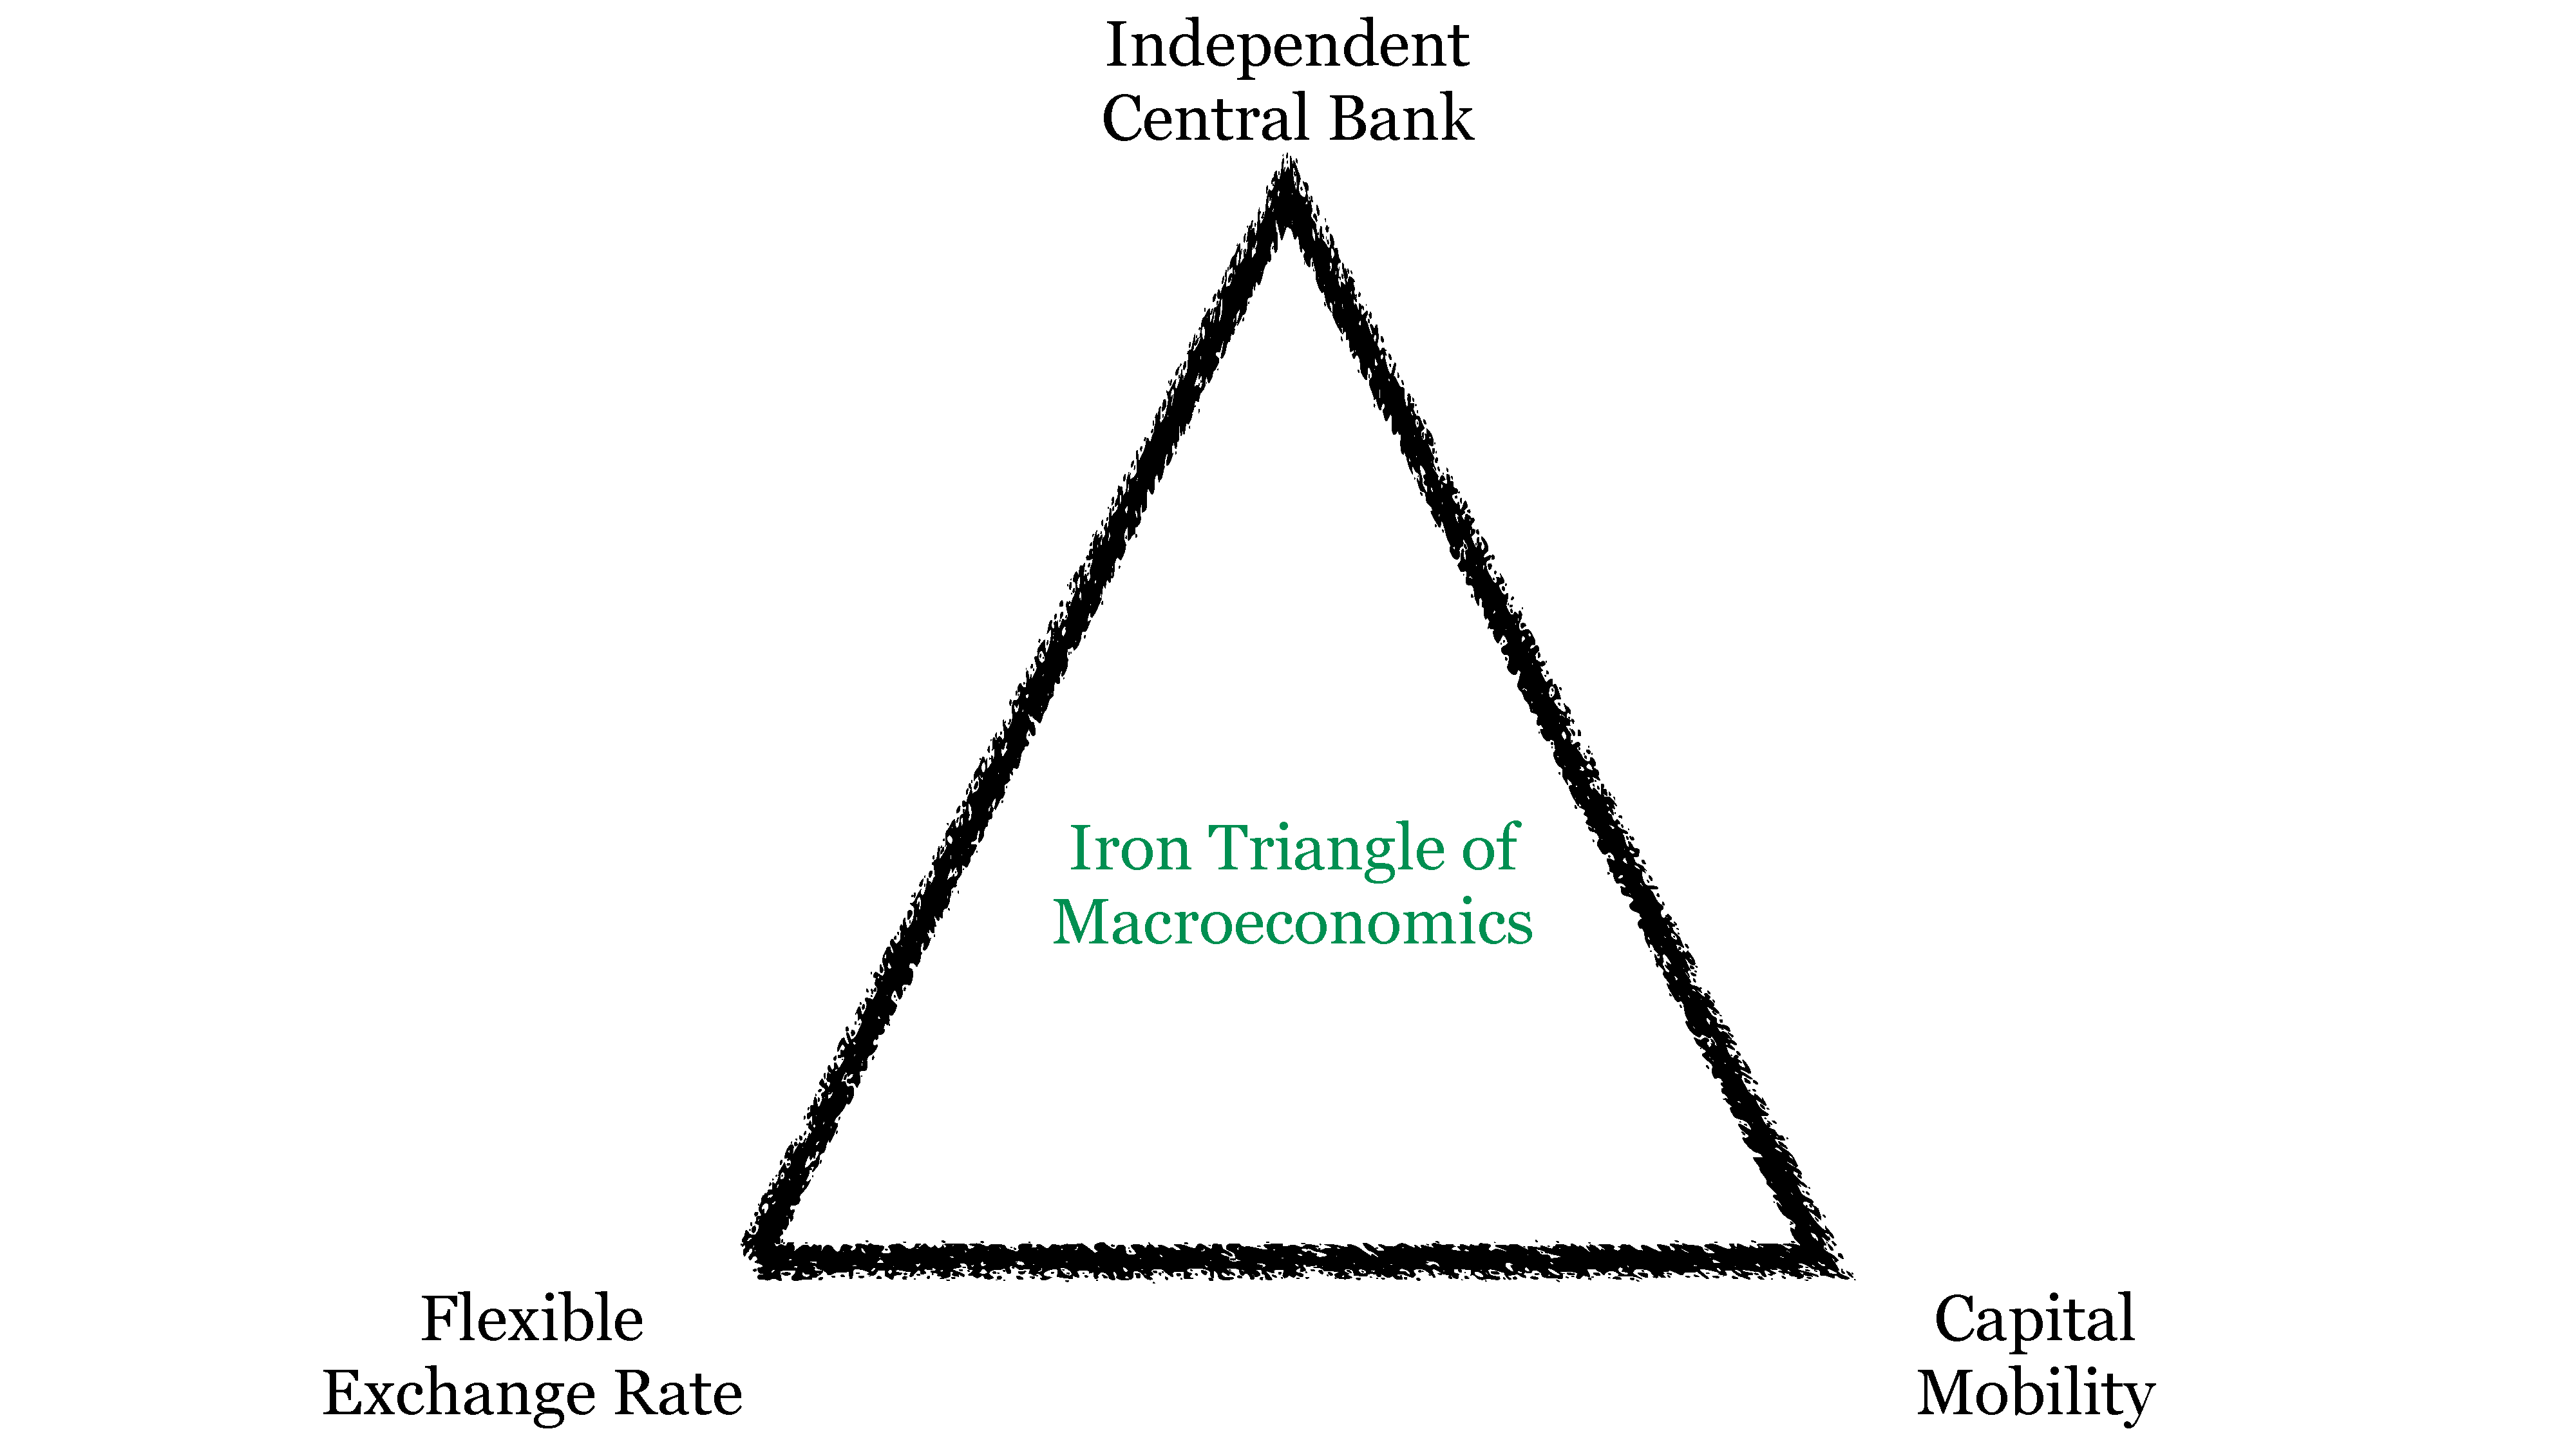
\includegraphics[width=1\linewidth]{triangle-macro}  
	\caption{The Iron Triangle of Macroeconomics}
	\label{fig:triangle-macro}
\end{figure} 

In the \gls{EU}, free capital movement is a given, and if convergence is to continue it must remain so \citep{Abiad2007}. The common market, indeed, is the minimal substrate if regional integration is to mean anything. With that corner of the impossibility triangle already occupied, \gls{EU} governments can only choose between fixed exchange rates or independent monetary policy. If governments wish to retain monetary sovereignty, they have to accept free exchange rates and any resultant volatility. If and to the extent that governments wish to limit exchange rate volatility, they \emph{must} coordinate their monetary policy, that is, enter a currency union.

\paragraph[Fiscal-CPR]{Common Pool Resource Problem.} \phantomsection \label{sec:Fiscal-CPR} If, to stabilize exchange rates, a common market must beget a common currency, to limit budget deficits, a common currency must also beget a common fiscal policy (Feldstein 2005: 7 as cited in \citealt{Begg2008}: 13). 

Without it, a common currency creates a \gls{CPR} of public debt. Inside the union, all \gls{MS} governments enjoy the low, average interest rates on its bonds. \glspl{MS} can feast on the common good of these low interest rates and take on large amounts of debt without the otherwise defining consequence of heightened interest rates as investors price in greater risk of default. %add link
Other union members may initially try to avoid any potential sovereign default, because in a highly integrated currency union, such defaults may cause systemic risks, especially with foreign union-level banks. Additionally, remaining union members may fear loss of investor confidence in the common currency if one of its members is allowed to default on its union-denominated debt. In particular, investors always worry that their sovereign bonds will be inflated away by debtor governments and therefore value a track record of sound fiscal and monetary performance not just in debtor governments, but in the entire currency, too. Currencies, in effect, are precious brands, vouching for the trustworthiness --- or lack thereof --- of the sovereign debt in which it is denominated.

Anticipating that other currency union members may want to bail out would-be sovereign defaulters, investors will downgrade the risk of any \gls{MS} debt and accept lower interest. Reacting on such incentives, \glspl{MS} may borrow more than they otherwise would or should, free-riding on the good reputation of other union members, they might eventually force to bail them out. As all currency union members face the full social cost of their sovereign debt, but the overall creditworthiness of the sum of all members naturally remains rival, choosing levels of sovereign debt at the \gls{MS} level becomes a common good: no one can be excluded from enjoying low, average interest rates, but overall solvency remains rival.

In a full fiscal union, this \gls{CPR} is resolved: the level of debt is decided at the same, highest level at which its costs eventually accrue. 

The \gls{EMU} --- seeking to counteract this moral hazard of communal interest rates --- originally forbade bail-outs, but that commitment, as it now shows, was not credible enough as Feldstein foresaw (2005: 7, as cited in \citealt{Begg2008}: 13). Absent any meaningful fiscal institutions to decide together, how much the union should raise, spend and dissave, the \gls{EMU} has fallen prey to its \gls{CPR}, or rather, its offending, extortionate, commons-exhausting members. 

%note (this is from somewhere, either Cassidy or Frank, probably frank, that more equality can make more Coase-style deals happen; that's what you want, be it in Coase-style property rights or Pigovian taxation. You don't want: having distributive stuff creep into commons et al. Good example: Pendlerpauschale in Deutschland.

%Background: Taxation Trends in the European Union

	%The Directorate General for Taxation and Customs Union issues an annual report on taxation in the European Union. Results from the 2009 edition include:
	%Tax ratios in the EU-27 remain relatively high (39.8% of GDP), but differ greatly between old and NMS (Romania 29.4%, Denmark 48.7%).
	%NMS raise relatively more revenue by indirect, non-redistributive taxes in immobile bases.
	%Almost all member states increase the (indirect) burden in (relatively immobile) consumption through VAT and excise duties. 
	%Top average (not marginal) Personal Income Tax (PIT) rates (37.8%) are in decline across almost all EU member states, but continue to vary dramatically between old and NMS (Bulgaria 10%, Denmark 59%).
	%Corporate Income Tax (CIT) rates are in rapid decline, from 35.3% in 1995 to 23.5% now. Again, NMS tend to have lower tax rates than older member states. 
	%Implicit Corporate Income Tax rates (CIT-ITR) are however, stable if diverging, possibly due to cyclical effects, base broadening or cannibalizing on the PIT.

	%Is there European (Corporate Income) Tax Competition?

	%In a liberalized Single Market, where capital and, to a lesser extent, labor through trade, investment and migration flow to their most profitable use, it appears reasonable to assume that these factors of production will also respond to taxes. Investors and workers will, as much as they can, flock to locations where tax rates are lower than the respective costs of relocation. To sustain output and growth, states would then have to compete for factors of production with low tax rates.

	%Before turning to the central question of whether this would be a desirable or undesirable dynamic, first ask whether it is real, and if so, how it came about.

	%Genschel, Kemmerling and Seils (2009) suggest (corporate income) tax competition is shaped by four interrelated institutional mechanisms of the EU:
	%Market integration (↑) reduces transaction costs of cross-border arbitrage (think: exchange rate volatility, tariffs) and thereby facilitates tax competition.
	%Enlargement (↑) adds new, attractive markets: new members are diverse in size (!) and economic development (GDP/Capita). Smaller and poorer countries have greater incentives and possibilities to lower taxes.
	%Tax coordination (↓) makes taxation more similar, and therefore reduces the ways in which governments can compete for capital and labor.
	%Supranational judicial review (↑) enforces the non-discriminatory liberalization (think: Cassis de Dijon) and limits the ability of governments to unilaterally defend against tax competition (think: Tobin Tax).

	%Genschel et al. find that tax competition is different and greater within the European Union than outside of it, and that it accelerates with time and enlargement.

	%They also suggest that larger countries suffer disproportionately from tax competition as smaller countries can boost their revenues (and growth) with the low rates on the massive inflowing capital from larger neighbors. Conversely, poorer countries have greater incentive and ease to compete for scarce capital.
	%The competition is less harsh amongst (now delegitimized) preferential tax regimes (PTR) (think: Hong Kong). When countries target only the most mobile of factors with tax breaks, the overall revenue effect tends to be smaller and more symmetric.

	%(A Prisoner's Dilemma Game of Tax Competition. Payoffs are tax revenues#.)

	%If these empirical results are correct, EU tax competition can be modeled as a Prisoner's Dilemma game, where states (strictly) dominantly prefer low taxes over high taxes and (Nash) equilibriate in suboptimal, mutual low taxation.


	%The Case against European Tax Competition: It's a Race to the Bottom

	%The argument against European tax competition builds on the assumed Prisoner's Dilemma dynamic, and suggests that EU states may not only be incapable to maximize public revenue under competition, but that thereby depressed tax revenue will lead to debt crises, the underprovision of public or common goods and impaired redistributive ability or a retrenchment of the Welfare State. It could also be argued that a harmonized European Tax regime better equips member states to withstand shocks with countercyclical tax and spend policies.

	%A related argument can be made about a presumed inability to respond to structural misalignments caused by liberalization. When trade, migration and investment allow countries to specialize even more according to their factor endowments (think: Romanian Nokia, German Management Consulting), remaining, relatively scarce factors (think: unskilled laborer in Germany) may find their market wages# fall even further below the respective socially acceptable minimum income#. Rich states may then be forced to redistribute income to these individuals, but find themselves unable to raise the necessary revenues (progressively) without further reducing their competitiveness. Tax competition could then exacerbate vicious dynamics of structural unemployment.

	%Tax competition is harshest on tax bases (capital, labor, firms) that are highly mobile (think: private equity). EU member state tax codes may be forced to converge on certain kinds of taxes. To appreciate this possibility, consider the qualities of different redistributive-/general-revenue taxes#.

	%(reproduced from Genschel 2007: 11) (whatever this was?)
	\chapter[Tax Matters]{Why Tax Matters to the Welfare State}
		\label{chap:tax-matters}
		%!TEX root=../tax-democracy-held.tex

\begin{quote}
	\emph{``The spirit of a people, its cultural level, its societal structure, the deeds its policy may prepare --- all this and more is written in its fiscal history, stripped of all phrases.
	He who knows how to listen to its message here discerns the thunder of world history more clearly than anywhere else.''}
	\\*
	--- Joseph Schumpeter (1918 [1991])
	%add complete quote
\end{quote}

%note from new yorker article how jk galbraith said that the rich should erect a statue to the PIT, because it allows great income inequality.
%Note to that that things might have changed today

%Some introduction of why tax matters, what this thesis looks at.

	% it is by the states capacity to reallocate market equivalent incomes that the welfare retrenchment should be all about, and that is:
%reallocation WITHOUT debt of one form or another.
%Important:
%a welfare retrenchment test should be independent of how market outcomes are reallocated, be it through taxation, or whatever.
		%Hunch:
%welfare state is worse today.

\section{Why it Matters:\ The Welfare State as Mixed Economy}
	\label{sec:why-mixed-economy-matters}

\begin{quote}
	\emph{``Yes we can:
	to justice and equality.
	\\
	Yes we can:
	to opportunity and prosperity.''}
	\\*
	%better quote, anyone?
	%duplicate
	--- Barack H.\ Obama, Obama For America 2008
\end{quote}

%Moreover, economists like Nicholas Barr (20013, 2004) argue that social insurance programs step in where markets fail.
%Given (via Mau/Leibfried)

%this is a better, more systematic way to think about problems and welfare, otherwise we're just confused.

At this point, a reader may ask:
why would all, or even any of this, matter to the welfare state?

Materially possible and normatively desirable welfare states are, and must be thought of as, well-designed mixed economies, for at least three reasons:

\begin{enumerate}
	\item \emph{Engaging Complexity.}
	In a welfare state, \hyperref[sec:interface]{exchange and command modes of production and distribution, inevitably, complexly interact and easily produce unintended consequences} (p.~\pageref{sec:interface}).
	For example, a \hyperref[sec:prince-controls]{minimum wage may cause structural unemployment} (p.~\pageref{sec:price-controls}) and the \hyperref[sec:well-determined-incidence]{\emph{nominal} incidence of a tax will be entirely inconsequential} (p.~\pageref{sec:well-determined-incidence}).

	To eradicate today, as Lord Beveridge promised 150 years ago, the five `Giant Evils' of want, disease, ignorance, squalor and idleness, you have to anticipate this interplay of market and government and choose accordingly.
	The mixed economy provides us with a toolset to analyze the complexity of welfare states, including the dynamics presented here.
	For example, the mixed economy suggests we should always check the \gls{dwl} (p.~\pageref{sec:minimal-DWL}) and \hyperref[sec:well-determined-incidence]{incidence} (p.~\pageref{sec:well-determined-incidence}) of any redistribution, a welfare state may undertake.

	To answer the first-order question of welfare state design, as I have here tried to do, we need the abstractions of the mixed economy to know what is \emph{materially possible} in a scarce world, filled with (at least some) homines oeconomici.
	For example, price controls may not be possible (without grave losses), but a well-designed, personal, almost arbitrarily progressive taxation \emph{is} indeed possible in a closed economy.

	\item \emph{Denaturalizing Market Allocations.}
	When we consider welfare state programs in isolation from the markets which they supplant, we easily end up naturalizing whatever markets have allocated.
	In fact, any given market exchange which a welfare state may seek to correct, is already and always \emph{contingent} on the institutions, dynamics and distributions under which it occured.

	For example, rather than ``fighting poverty'' --- as if that were an objective reality --- welfare states must consider overall allocative dynamics (such as \hyperref[sec:winner-take-all]{winner-take-all}, p.~\pageref{sec:winner-take-all}) and distributions (such as \hyperref[sec:monopsony-employers]{monopsony employers}, p.~\pageref{sec:monopsony-employers}), and counteract them, as is seen fair.
	Markets do not make some people below an arbitrarily defined threshold ``poor'', and leave others ok or even untouched.
	Instead, markets allocate incomes across the \emph{entire} spectrum contingent on a host of institutions, dynamics and initial distributions.
	If government pursues a particular minimum standard of living for everyone, it might not only transfer income to those who fall below it, but may need to counteract those dynamics under which people slipped below the minimum standard in the first place.

	Market allocations, in short, are --- and should be --- no less subject to enlightened, collective human choice than remedial welfare state programs:
	``Increasing dependency is no law of nature but the result of socio-economic changes, which in turn react to human intervention'' \citep[x]{Esping-Andersen2002}.

	\item \emph{Caring about Outcomes.}
	\citeauthor{Haggard2009} (\citeyear[236]{Haggard2009}) remind us about

	\begin{quote}
		\emph{``[\ldots]
		the importance of pushing the research on the [Eastern European] welfare state down the causal chain towards its social consequences.
		[\ldots]
		[A]ny meaningful strategy of comparison of the welfare state must ultimately engage its consequences for a variety of outcomes, from poverty and inequality, to physical quality of life measures, to economic outcomes such as the efficiency of labour markets, competitiveness and even economic growth.
		In the first instance, we are interested in the welfare state because we are interested in human welfare.''}
		\\*
		--- \citet*[236]{Haggard2009}
	\end{quote}

	The abstractions of the mixed economy I have summarized here synthesize a lot of what we need to know about the material, and therefore social consequences of a capitalist welfare state.

	When we care about social consequences, the mixed economy suggests a great deal more to consider than just nominal welfare programs.
	For example, welfare states should not only provide social insurance, but also redress failing \hyperref[sec:public-good]{public goods} (p.~\pageref{sec:public-good}) and \hyperref[sec:long-term-inconsistency]{make us save enough for our children} (p.~\pageref{sec:long-term-inconsistency}).

	When we care about social consequences, the mixed economy also implies that not all welfare programs are created equal.
	For example, welfare states interventions should \hyperref[sec:minimal-DWL]{distort market prices as little as possible} (p.~\pageref{sec:minimal-DWL}) and use \hyperref[sec:price-stability]{monetary expansion only sparingly, for short-term stimulus} (p.~\pageref{sec:price-stability}).

	When we care about social consequences, the mixed economy suggests that  governments and markets are better at different things, and it ties welfare state interventions to specific justifications.
	For example, welfare states should nationalize or regulate utility markets if and to the extent that they are \hyperref[sec:natural-monopoly]{natural monopolies} (p.~\pageref{sec:natural-monopoly}), but there is no reason to (as Germany presently does) redistribute within \hyperref[sec:state-insurance]{social health insurance} (p.~\pageref{sec:state-insurance}), who was supposed to only save the risk pool from \hyperref[sec:adverse-selection]{adverse selection} (p.~\pageref{sec:adverse-selection}).
	Caring about social consequences also means to leave markets alone, if they will likely serve material human need best.

	When we care about social consequences, the mixed economy reveals that efficiency and equity are not always opposed, but often go hand in hand.

	\begin{enumerate}
		\item \emph{Inefficient is Inequitable.}
		\citeauthor{Titmuss1974} urged welfare states not to exclusively concentrate on poverty relief because such ``residual services (\ldots) often become poor services for poor people'' \citeyearpar[134]{Titmuss1974}.
		This intuition is supported by the abstractions of the mixed economy:
		as the rich are forced or allowed to take the inefficient --- but for them, affordable --- exit route from government provision, a retrenched welfare state will offer only inferior provision, or none at all, to those too poor to exit.

		This problem is particularly acute in health or disability insurance:
		as the rich and healthy exit the risk pool, coverage becomes ever more expensive, driving even more people out until it \hyperref[sec:adverse-selection]{fails} (p.~\pageref{sec:adverse-selection}).

		Similar distributive effects occur in a wider class of market failures, too.
		For example, a failed \hyperref[sec:common-good]{commons} (p.~\pageref{sec:common-good}) of global climate or local public safety will not only be wastefully inefficient, but it will also hit hardest the poorest regions and people, who can least afford substitutes, such as building a levee or hiring private protection.

		\item \emph{Inequitable is Inefficient.}
		On the other hand, the abstractions of the mixed economy also imply that sometimes, slicing the pie unequally, will also make it smaller:
		``(\ldots) there is a very good argument that equality of opportunities and life chances is becoming sine qua non for efficiency as well'' \citep[ix]{Esping-Andersen2002}.

		For example, people may not be able to align the \hyperref[sec:principal-agent-problem]{interests of principals and agents} when collateral is not widely available (p.~\pageref{sec:principal-agent-problem}), and overly taxing low and middle (labor) incomes may contribute to \hyperref[sec:minimal-DWL]{structural unemployment} (p.~\pageref{sec:minimal-DWL}).
	\end{enumerate}

	To answer the first-order question of welfare state design, as I have here tried to do, we need the abstractions of the mixed economy to know what is \emph{normatively desirable} in a scarce world, filled with (at least some) homines oeconomici.
\end{enumerate}

\paragraph[Higher Equilibria]{Higher Equilibria.}
The first-order conflict about the best, possible welfare state is about the trade-offs, contradictions and uncertainties of the mixed economy explained in the above.
My aim here was not to resolve that conflict:
we may not know for sure, let alone agree on what \emph{the best} welfare state looks like (even though I offered some well-informed hunches).
A mixed economy can --- in principle and for my purposes here --- make \emph{arbitrary} trade-offs between equity and efficiency, presence and future, or any of the other dimensions of human material need.

	%3) There are inevitable contradictions in todays political economy of fighting the dynamics of inequality which the welfare state is systematically, (one wonders:
%on purpose?) ill-equipped to adress.
%(think income taxation)

But given \emph{any} preference set for these (sometimes!) competing goals, there are still more and less efficient institutional configurations for the mixed economy.
More efficient, in this broadest sense, means that these configurations achieve more on \emph{all} goals.
These preferable mixed economies will still trade off preferred goals for less preferred goals, but the trade-off will be less harsh.
For example, a \gls{nit} may achieve the same, if not more equity than a minimum wage, but at much lower cost in growth, or unemployment.
Of course, you still have to break eggs for the proverbial omelette, just fewer of them.

% here used to be \ref{fig:ppf-values}, which is now gone only in wanted.

%DUPLICATE!!!%
\begin{figure}[htbp]
	\centering
	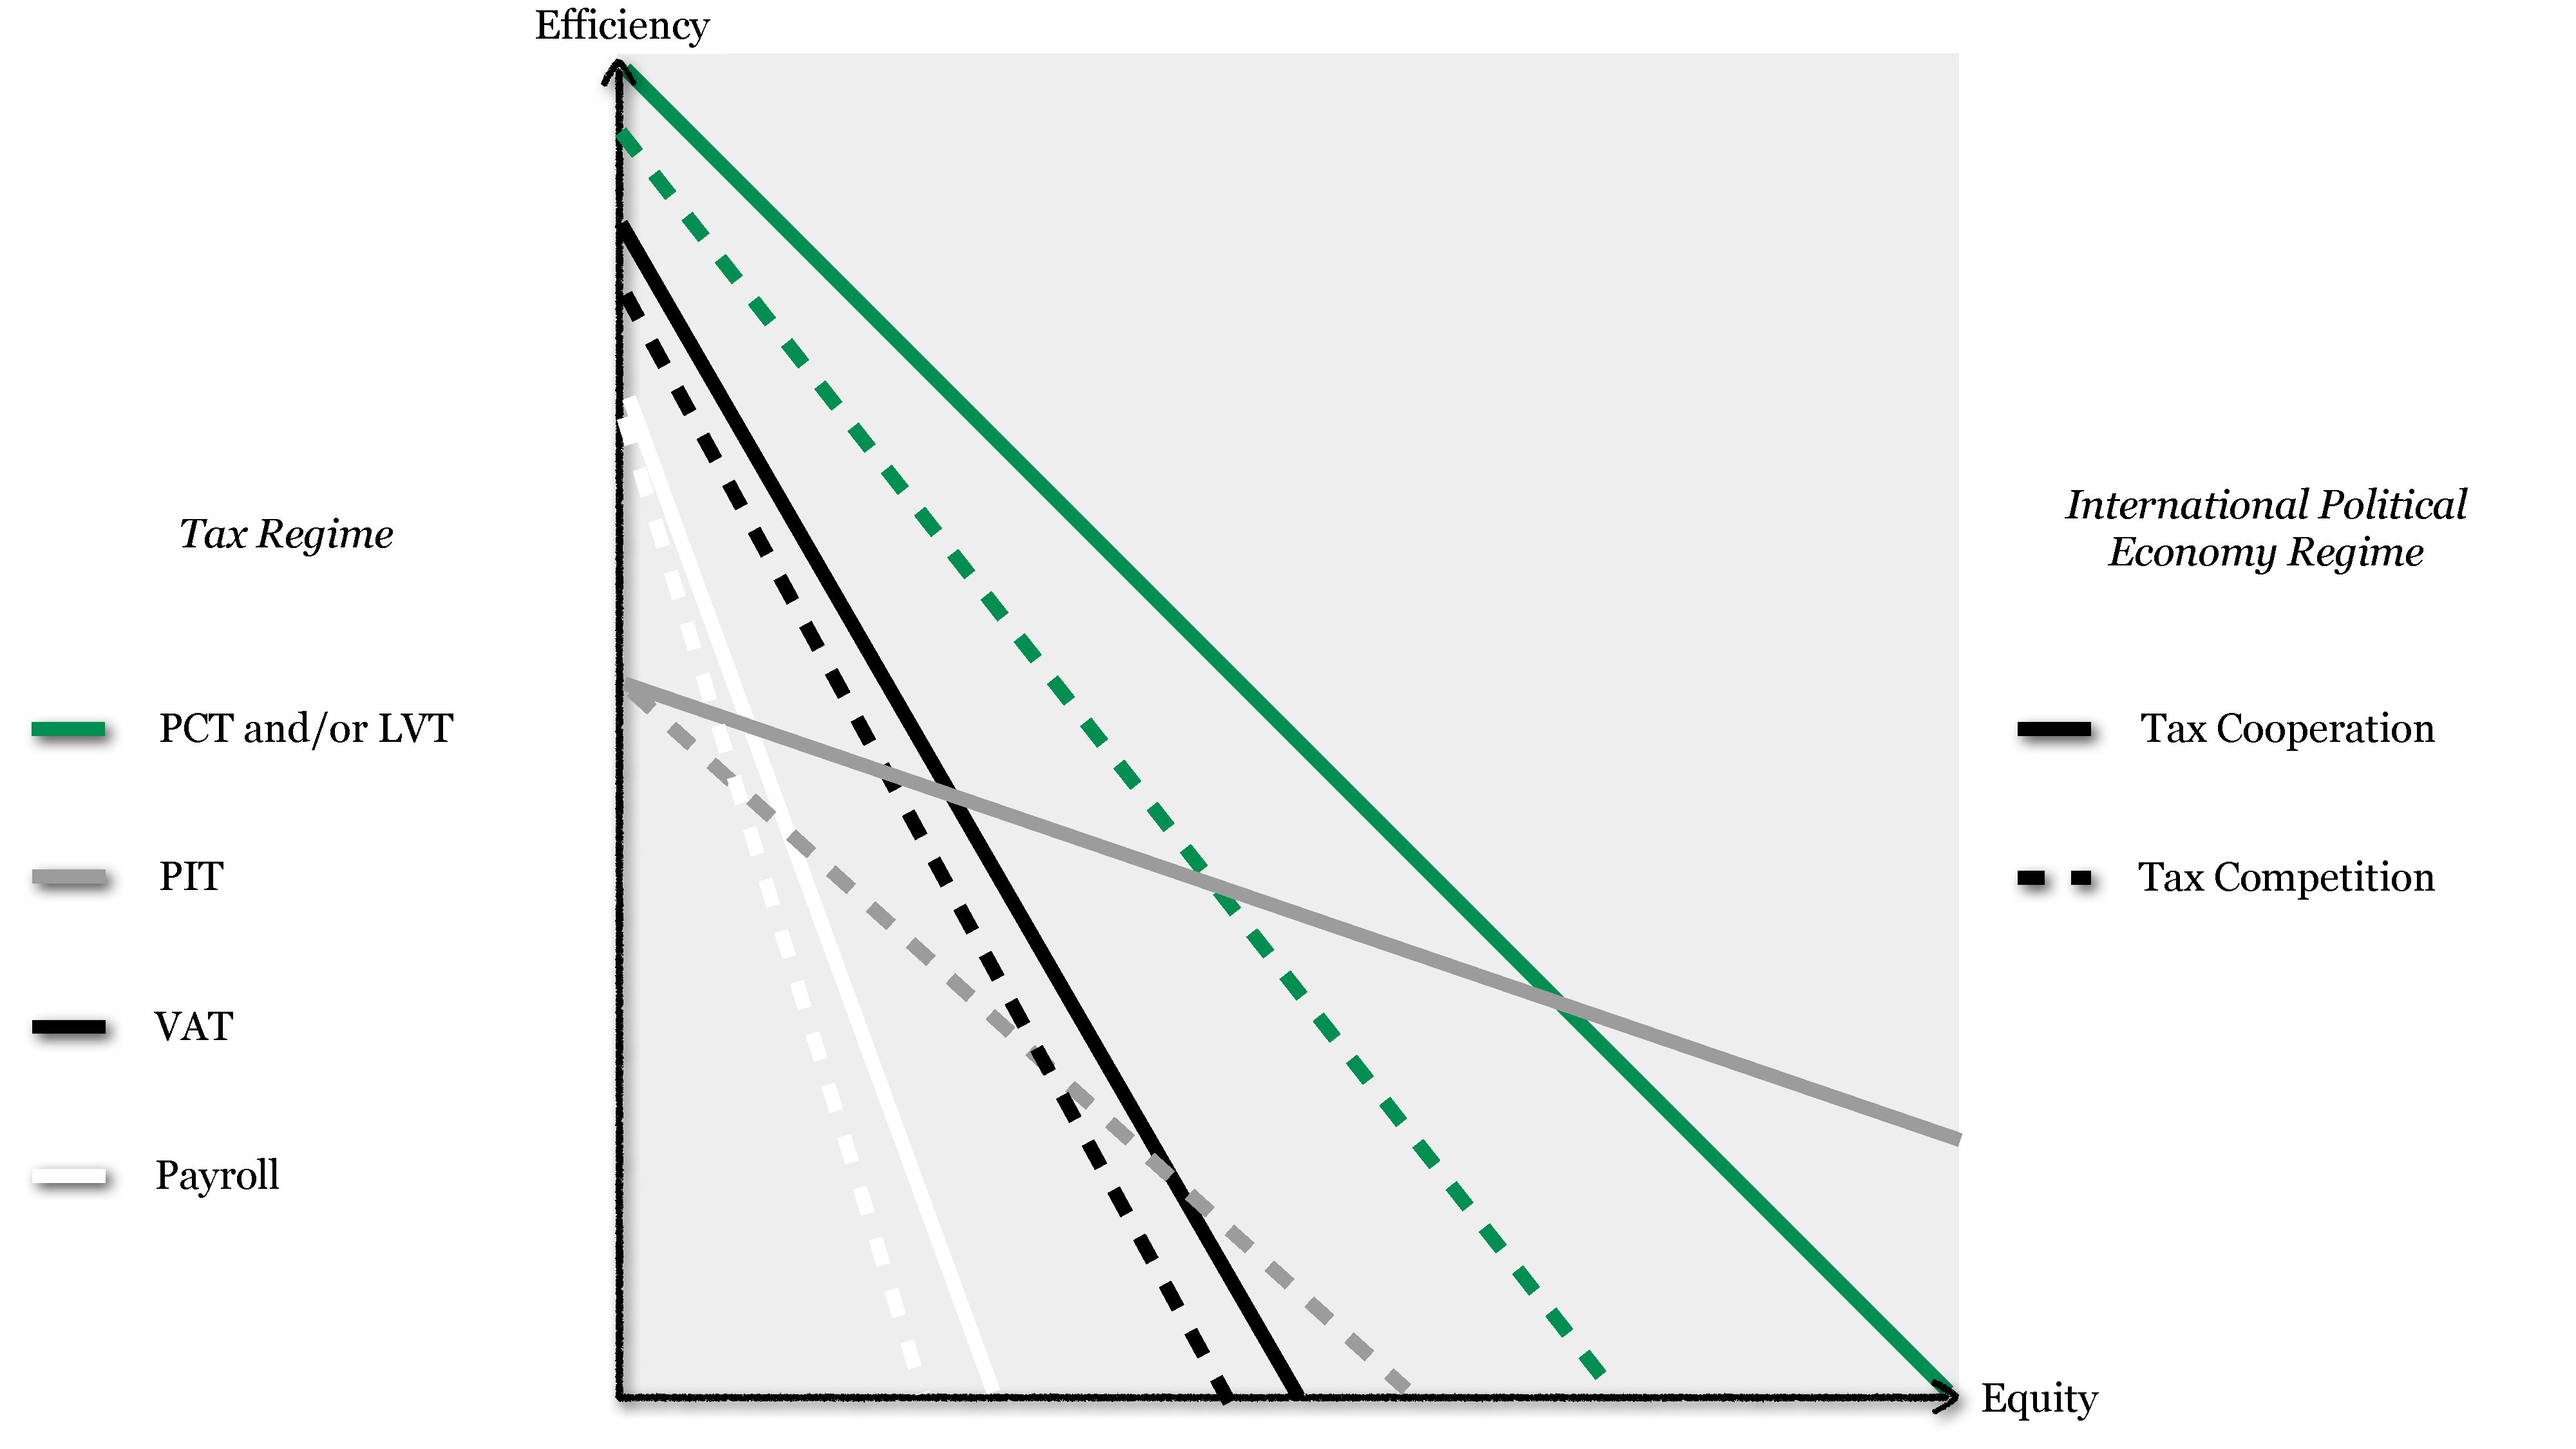
\includegraphics[width=1\linewidth]{ppf-tax-regimes}
	\caption[Equity-Efficiency Trade-offs of Different Tax Regimes]{A Production Possibilities Frontier of Equity and Efficiency in Different Tax Regimes}
	\label{fig:ppf-tax-regimes} %add compare footnote to \ref{fig:ppf-values}
\end{figure}

The competing goals of human material need, in other words, are not always in a pure and immutable zero-sum relation, where, for example, one increment more in equity means one less in efficiency, one more in present consumption one less in future consumption.
Depending on the institutional design, these conversion rates will differ:
sometimes, for example, one increment in equity will cost only a half-increment in efficiency.
Alternative mixed economies, more often than not, are a positive or --- equivalently --- negative sum proposition.

Just entering the preferences between purposely competing goals does \emph{not} yield a single configured mixed economy, but many different blends of command and exchange production and distribution.
Again, we may not know or agree what the globally optimal configuration is, given our preferences, but checking \hyperref[sec:means]{means} and \hyperref[sec:ends]{ends} of a mixed economy, we \emph{can} know better from worse configurations, or local optima.

A better welfare state is that mixed economy which elegantly combines \hyperref[sec:command]{command} and \hyperref[sec:exchange]{exchange} components to \hyperref[sec:production]{produce efficiently}, \hyperref[sec:risk]{pool risks}, \hyperref[sec:distribution]{distribute equitably}, \hyperref[sec:time]{consistent over time} and \hyperref[sec:space]{convergent over space}.
That is, a welfare state that offers one of the higher possible trade-offs of growth, individual security, equality, saving and convergence.
It does so without effectively borrowing from the future through \hyperref[sec:smoke-n-mirrors]{smoke and mirrors}, or hidden, but \hyperref[sec:real-dissavings]{real dissavings}.

%Do I need the next section in the thesis?
%It might not fit.

This view of the welfare state differs markedly from other perspectives:
\begin{description}
	\item[Full Employment or Growth.]
	A popular variant on the purposive trade-off between equity and efficiency, is that between the policy goals of full employment or growth, sometimes supported by ``demand-'' or ``supply-side'' economics.
	%make a footnote about this.
	%might need a bigger section about this, maybe with bastard keynesianism.
	\citeauthor{Offe2003} \citeyearpar[453]{Offe2003} finds a similar controversy about how to best keep up the full employment ``roof'' over the metaphorical Keynesian welfare state house, protecting the lower floors:
	market liberals (or supply-siders) want to deregulate so that \emph{growth leads to more employment} and social democrats (and, sometimes, demand-siders) want to sustain welfare state protection so that \emph{more employment stimulates growth}.

	These contenders both once had a (somewhat overstated) point, but as market failures grew and monetary policy improved, they are now both increasingly wrong.

	Market liberals are wrong because not all deregulation, or any amount of it, will stimulate growth, and conversely, not all redistribution or other intervention will depress growth.
	The abstractions of the mixed economy suggest that sometimes, command production is more \hyperref[sec:market-failures]{efficient} (p.~\pageref{sec:market-failures}).

	Social democrats, or more accurately, demand-siders are wrong because, of course, in the long run, \emph{only} supply determines prosperity, and the depressed aggregate demand they \emph{always} seem to suspect is clearly defined as a monetary phenomenon and unlikely to persist for very long.
	If it occurs, monetary expansion and fiscal stimulus should smooth it out, but that does not make for a roof.
	Social democrats are also wrong to believe that all redistribution and regulation is cost-free:
	there \emph{are} \glspl{dwl}.

	The indicators of \emph{activity} that both market liberals and social democrats usually obsess about --- \gls{gdp} and full employment respectively --- are both emphatically not related to greater \hyperref[sec:trade-offs]{Haig-Simons incomes} (p.~\pageref{sec:trade-offs}).
	And so, they both sometimes fall for \hyperref[sec:smoke-n-mirrors]{smoke and mirrors} (p.~\pageref{sec:smoke-n-mirrors}) and ignore \hyperref[sec:real-dissavings]{real dissavings} (p.~\pageref{sec:real-dissavings}).
	%reference earlier footnote.

	So how can we rescue full employment?
	By \emph{not} fighting this last war, for at least two reasons.

	\begin{enumerate}
		\item Pushing macroeconomic policy to full employment risks overheating the economy and building up inflationary pressure.

		\item More fundamentally, full employment no longer is (if it ever was) a necessary, let alone sufficient factor for anything we might consider socially desirable outcomes for a welfare state.
		Full employment in itself cannot, as the house metaphor suggests, provide any shelter for depleted \hyperref[sec:common-good]{commons}, lemon-market \hyperref[sec:adverse-selection]{risk pools}, let alone address intertemporal failures or bubbles, to name just a few.
		More dearly to social democrats, full employment will also be increasingly unable to --- as the proponents of power resources had hoped --- level the playing field between capital and labor, simply because some of the major inequities no longer are between capital and labor, but also \emph{within} labor incomes as \hyperref[sec:winner-take-all]{winners-take-all} (p.~\pageref{sec:winner-take-all}).
		Even if the ``reserve army of the unemployed'' is fully activated, the resulting upward pressures on low (or all) wages will be no match for the governing dynamics of inequality enveloping the postindustrial economy (such as Baumol's cost disease).
	\end{enumerate}

	Full employment, and (properly defined) growth are still desirable --- because they are an efficient \emph{outcome} --- but neither serves as a powerful \emph{instrument} to reduce poverty or economic insecurity:
	``Promoting labour market participation is no substitute for income redistribution and the fight against poverty:
	more work does not necessarily mean less poverty'' \citep[ix]{Esping-Andersen2002}.
	\citeauthor{Offe2003}'s metaphorical house of the Keynesian welfare state, in other words, does not need a few new shingles, but an altogether new roof.

	That new roof is the ability of the mixed economy to redistribute, efficiently and progressively as the democratic sovereign wishes.
	With that ability, welfare states can subsidize any (however small) minimal labor market income to any desired minimum standard of living (for example, through a \gls{nit}), and can provide any level of social protection desired without counterproductively burdening low incomes (for example, by paying social insurance out of general tax revenue).
	Progressive redistribution could, if desired, dampen or counteract any existing income dynamic, including \hyperref[sec:winner-take-all]{winner-take-all} markets.
	\citeauthor{Offe2003} may be right that the welfare state did not ``have much to do with `equality of outcomes' '', but that does not make it tenable or desirable today \citeyearpar[450]{Offe2003}.
	If you are serious about even just ``security and protection of workers, not equality'' (\emph{ibid.}) you have to care about inequality and redistribution, at least a little.
	Without it, you will not have the resources to guarantee even such minimal, unequal outcomes for workers.
	I further develop this argument  in my \hyperref[sec:Pangloss]{Panglossian} critique of the literature (p.~\pageref{sec:Pangloss}).
		%this might need to be consolidated with the re-entrnechement part.
		%Voltaire:
	%     The rich require an abundant supply of poor.

	\item[Decommodification]
	still serves well to distinguish different welfare states \citep{Esping-Andersen-1990-aa}, but it, too, is no strategy for a possible and desirable mixed economy.
	Of course, welfare states may still ``decommodify'' (or \emph{subsidize}) health care, education and replace (or \emph{insure}) the incomes of the sick, disabled, old and unemployed, but such programs may be better described in the language of the mixed economy:
	as \emph{specific} market interventions and redistribution.

	The difference is not merely semantic, but at least three substantial misunderstandings easily follow from this choice of terminology:
	\begin{enumerate}
		\item Decommodification suggests --- misleadingly --- that welfare states \emph{could} take some aspects of life, and some people \emph{off} the market.
		But, because command and exchange modes of production and distribution always interact, that cannot be done.

		For example, decommodification of disability income is easily misconstrued to mean that disability would no longer be affected by the market, and that markets would no longer be affected by disability.
		That is not so.
		When welfare states support the disabled, they not only exempt them --- as intended --- from earning a market income, but they may also make it cheaper, and therefore more likely for labor markets to \emph{produce}, say, burn-out, depression or back pain.

		Thinking in the abstractions of the mixed economy helps us to avoid such pitfalls.
		In this case, we know that \emph{insurance} of risks is prone to moral hazard, and that (Pigouvian) co-payments can save the commons of a prudent risk-pool.
		We can, if desired, slap a Pigouvian tax on risky or strenuous employment and activities, to make sure it is more costly, and is avoided.

		\item Decommodification easily morphs from description to prescription, as for example, when income replacement becomes a measure for welfare state re- or entrenchment.
		%add source
		Caring about outcomes, there is nothing inherently desirable or essential about decommodification, for four reasons:

			\begin{enumerate}
				\item To decommodify someone out of the market also means to exit someone out of the central institution, that aside from providing the substituted material sustenance, mediates much human cooperation, generates self-worth to many and allows people to shape the world around them, however marginally.
				Instead, we should ``enable all citizens to participate in the mainstream of social and economic life'' \citep[ix]{Esping-Andersen2002}.

				\item Complete decommodification is a last resort response to hardship.
				Mixed economies have several alternative, and less intrusive, approaches to, for example long-term unemployment.
				Instead of generous, universal and unconditional --- and therefore decommodifying --- benefits, a mixed economy may subsidize low market wages with a continuous and regressive \gls{nit}.

				The availability of a \emph{specific} tool, may not much matter to the desirability of a welfare regimes:
				social outcomes do.

				\item Decommodification, conceptually, if not always in reality, is ignorant of potential welfare losses, as some person is provided, or some activity done under command instead of exchange --- without a respective, justifying market dysfunction.
				Thinking instead, in the abstractions of the mixed economy, always ties a market intervention to a particular market failure or broader dysfunction, and considers the potential welfare losses.
			\end{enumerate}

		\item Decommodification is both radical as a prescribed tool (exit the market) \emph{and} strictly limited in its reach (only a set of included people or activities).
		To be sure, sometimes a complete move to (entitled) command provision and distribution may be necessary or desirable.
		Likewise, a democratic sovereign may choose to only care \emph{a lot} about some market outcomes --- and decommodify them ---, and not care about others \emph{at all}.
		But there is no reason that all welfare states should do so, let alone that we carve this specific vision of a social compact into our conceptual toolbox.
	\end{enumerate}
\end{description}

\paragraph{It follows:}
for a better welfare state to strike any such optimal balance, even given arbitrary preferences, it needs an intact set of \hyperref[sec:regulatory]{regulatory} (p.~\pageref{sec:regulatory}), \hyperref[sec:fiscal] {fiscal} (p.~\pageref{sec:fiscal}) and \hyperref[sec:monetary]{monetary} (p.~\pageref{sec:monetary}) \hyperref[sec:means]{means} of a mixed economy.
%this sentence could be better.

Of these, tax is the elephant in the room:
it is by far the most versatile, precise and powerful tool of command production and distribution in the mixed economy.

None of this is a merely abstract or academic concern.
Much lies this balance of command and exchange:
everything we materially value, and with that, a great deal of the life chances of us all depends on an intact mixed economy.

This is also not a revolutionary project.
It does not ask for a new man, but it accepts, and timidly merely reforms \emph{homo economicus}, the civilized version of our selfish demons.
It does not ask for a new institution, it carefully compromises existing ways of exchange and command.
The mixed economy, by any historical standard, is not a radical proposition.

This much, I hope, is widely agreeable.
%go back to europe piece to see what else might be missing

\begin{quote}
	\emph{``Taxes are the price we pay for a civilized society.''}
	\\*
	--- Oliver Wendell Holmes, Jr.\ (1904), Washington, DC
\end{quote}

%add comment, footnote:
%this was first submitted as \ldots

 \begin{figure}[htbp]
	\centering
	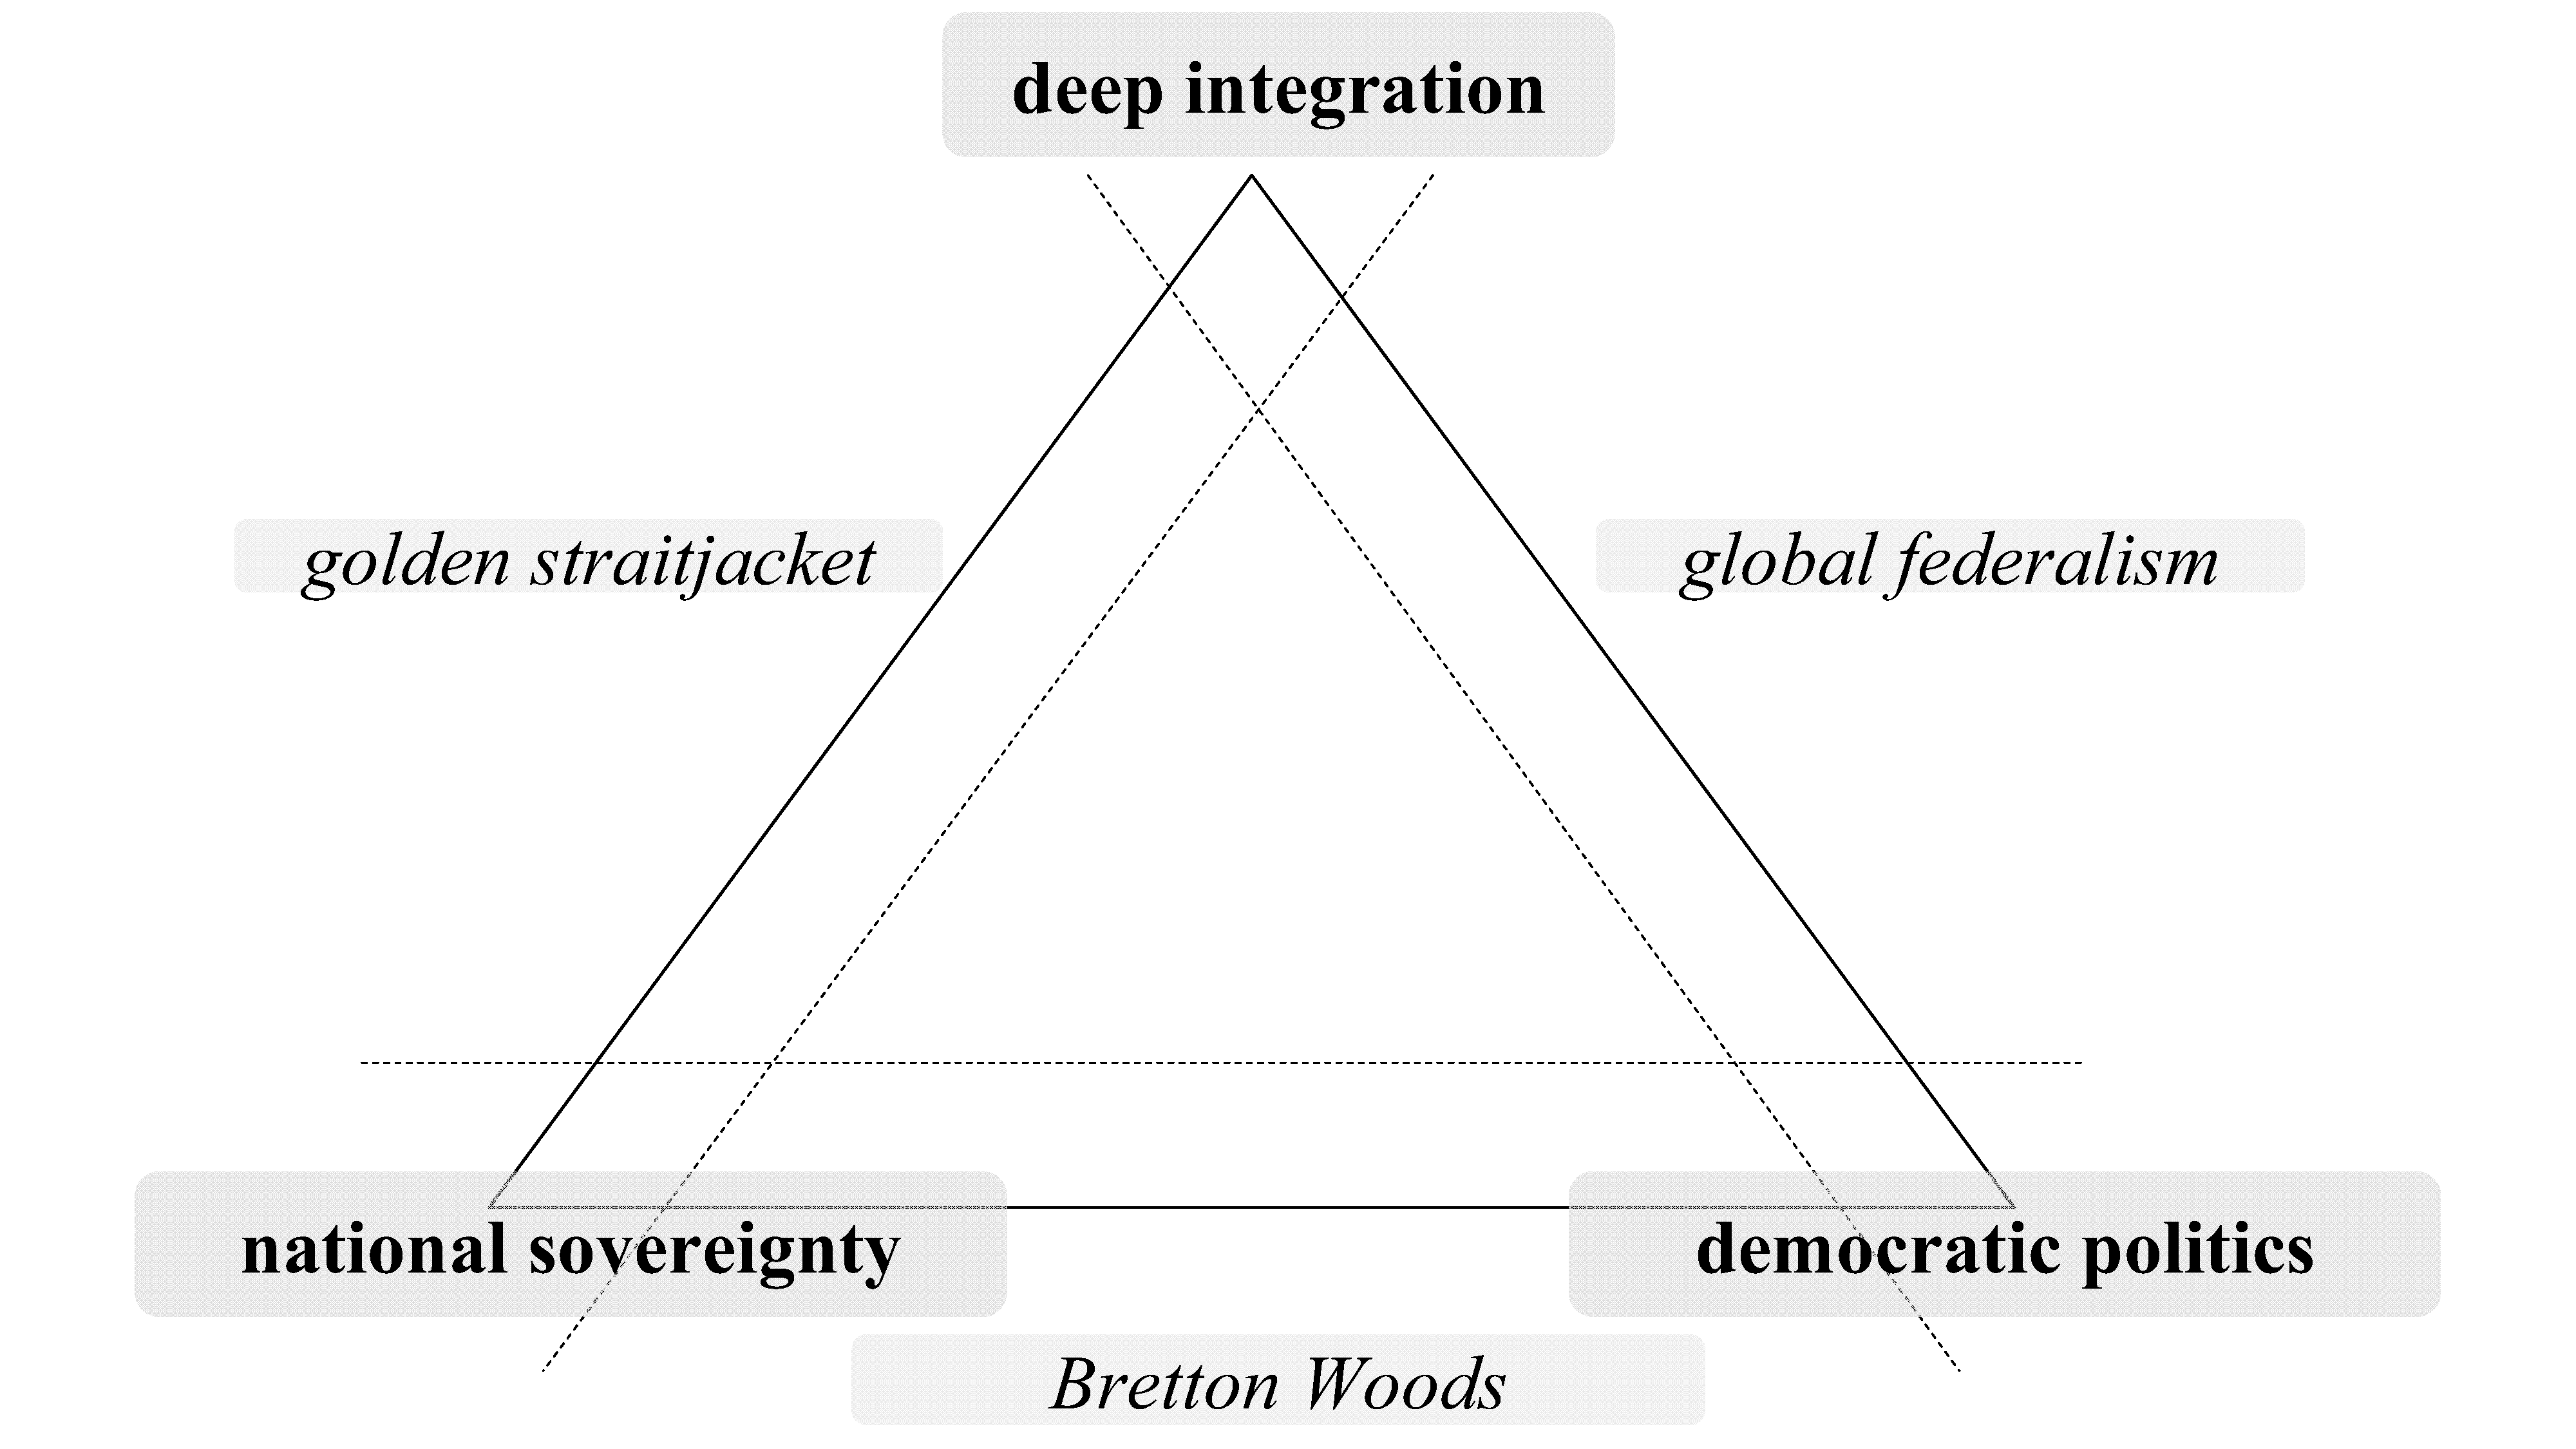
\includegraphics[width=1\linewidth]{ganssmann-macro-regimes}
	\caption{Macroeconomic Regimes and Political Priorities}
	\label{fig:ganssmann-macro-regimes}
	\begin{flushleft}
		\scriptsize{\cite{Rodrik2002} as reproduced in \citet[348]{Ganssmann2010}}
	\end{flushleft}
\end{figure}

\begin{figure}[htbp]
	\centering
	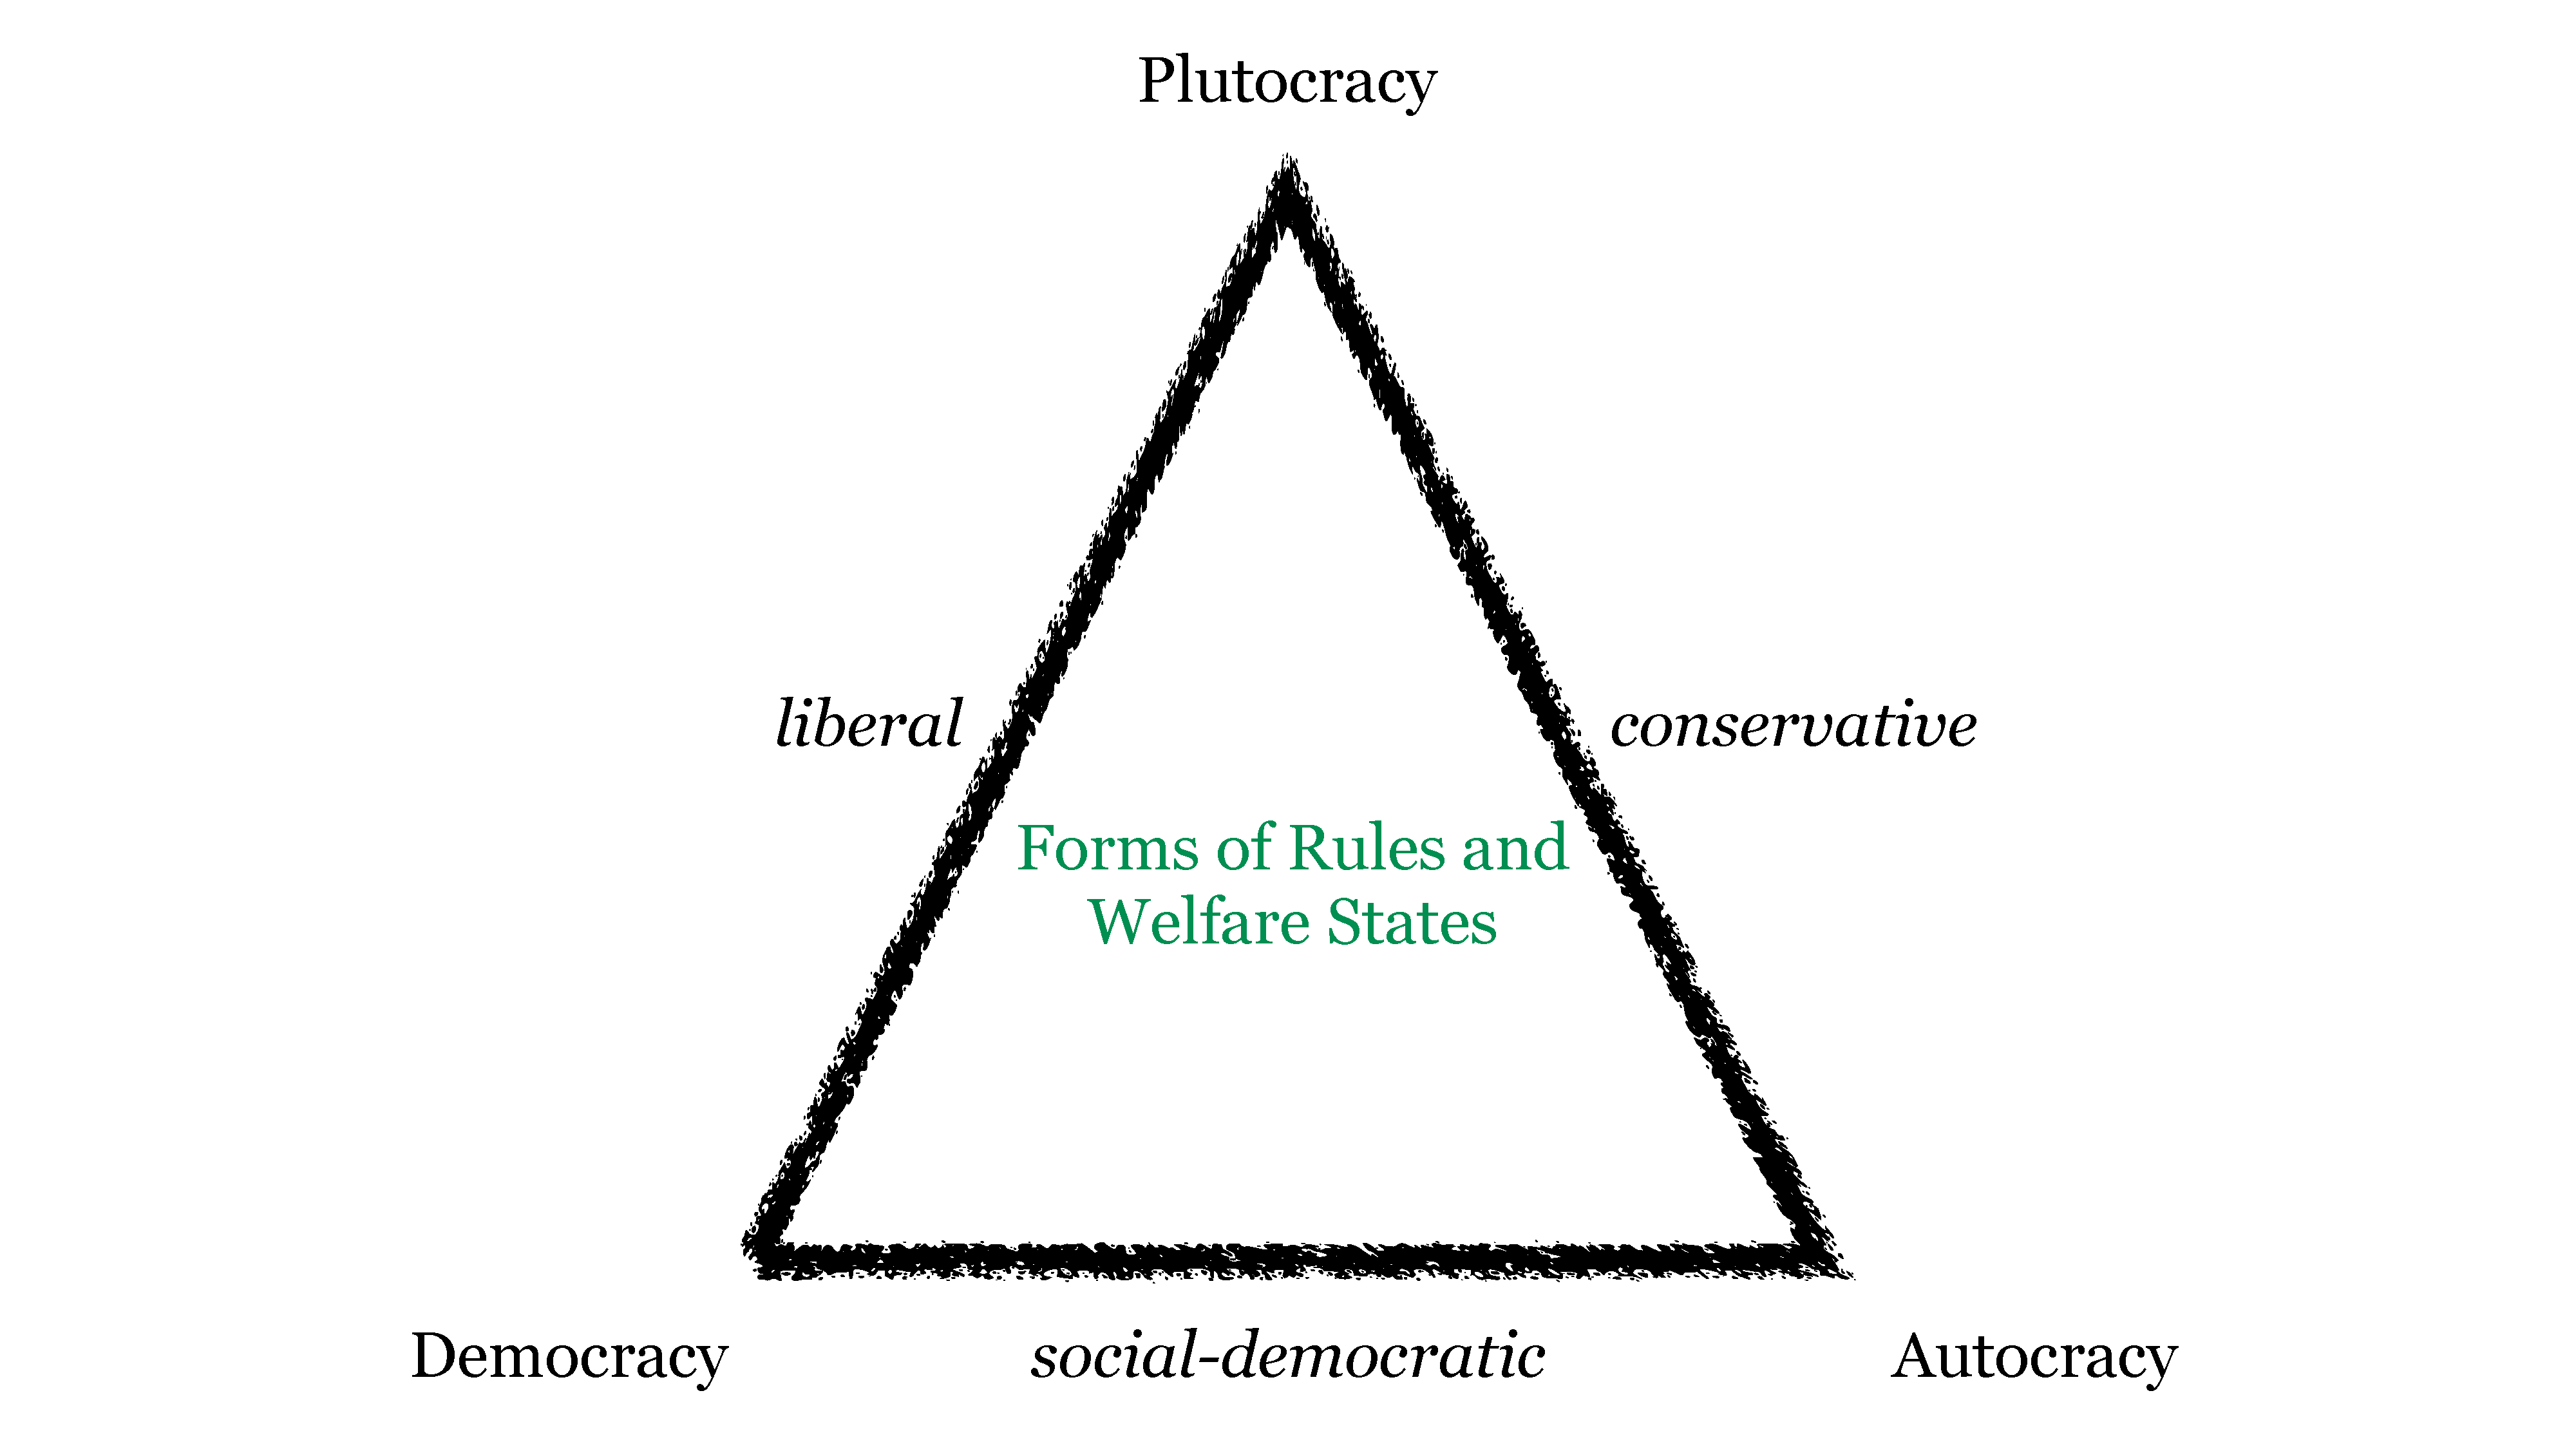
\includegraphics[width=1\linewidth]{ganssmann-rule-ws}
	\caption{Forms of Rule and Welfare State Regimes}
	\label{fig:ganssmann-rule-ws}
	\begin{flushleft}
		\scriptsize{Reproduced from \citet[334]{Ganssmann2010}}
	\end{flushleft}
\end{figure}

\begin{figure}[htbp]
	\centering
	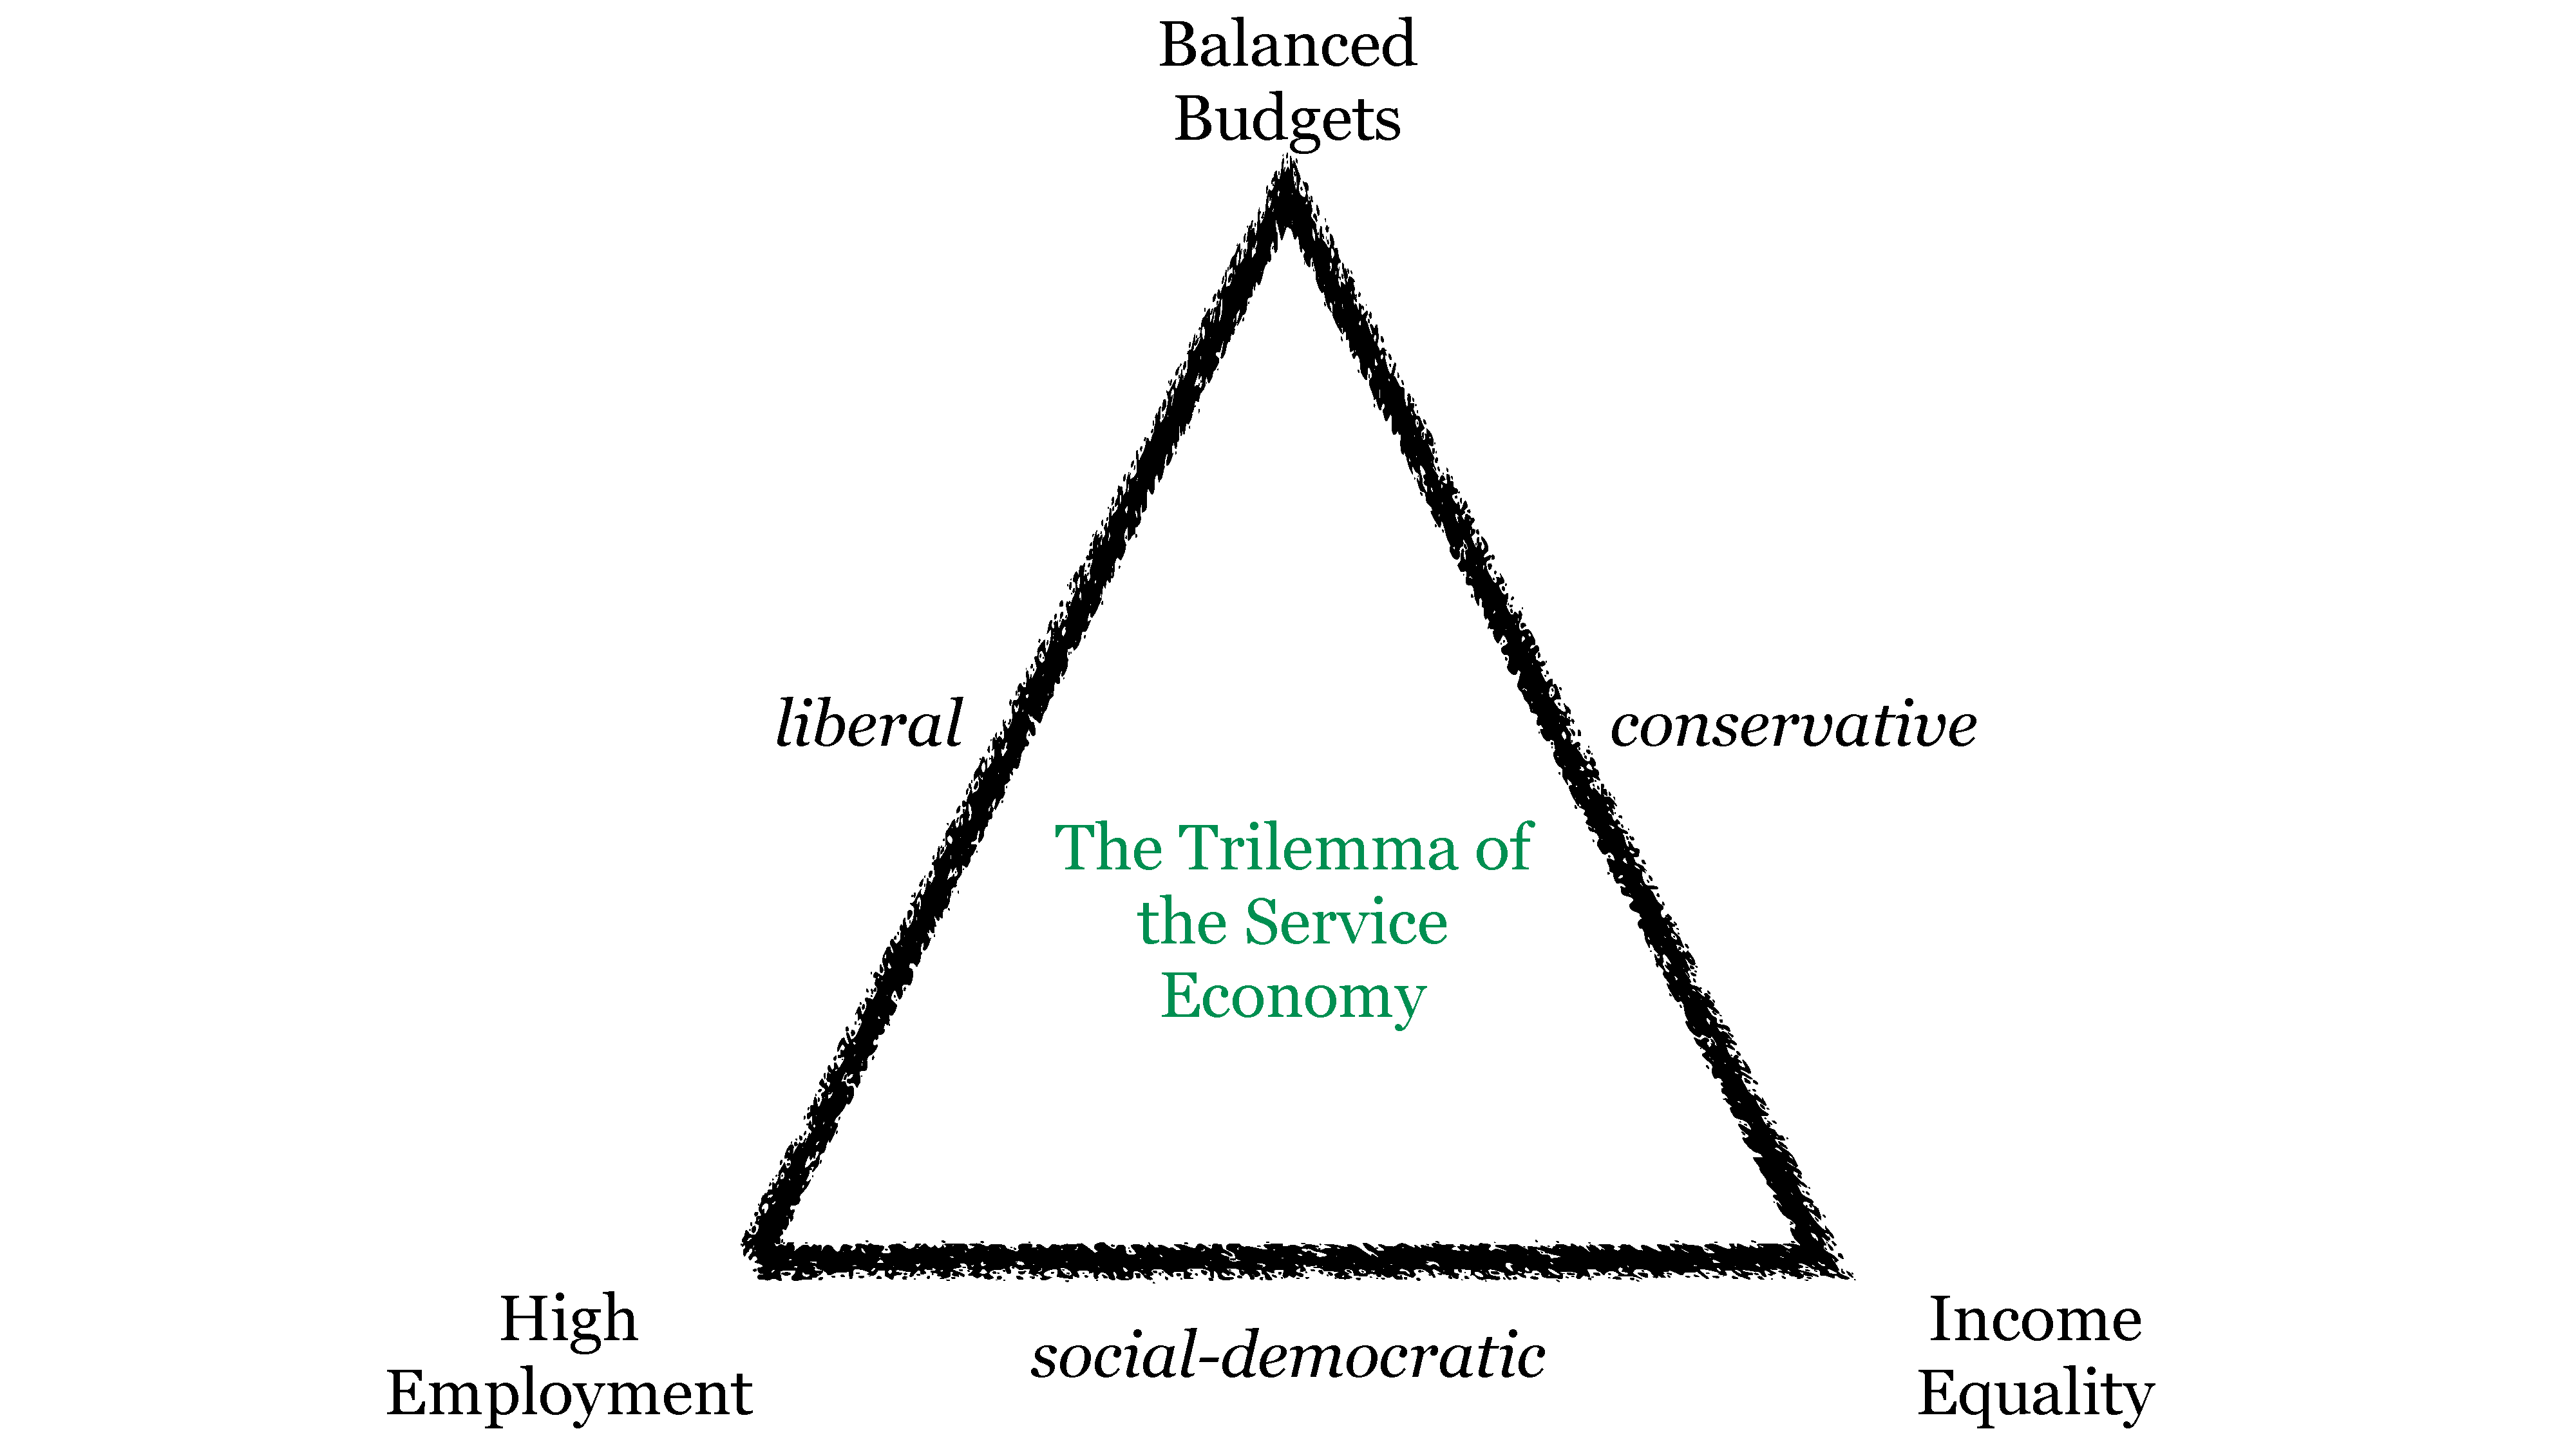
\includegraphics[width=1\linewidth]{ganssmann-trilemma-service-economy}
	\caption{Trilemma of the Service Economy}
	\label{fig:ganssmann-trilemma-service-economy}
	\begin{flushleft}
		\scriptsize{Reproduced from \citet[341]{Ganssmann2010}}
	\end{flushleft}
\end{figure}

\begin{figure}[htbp]
	\centering
	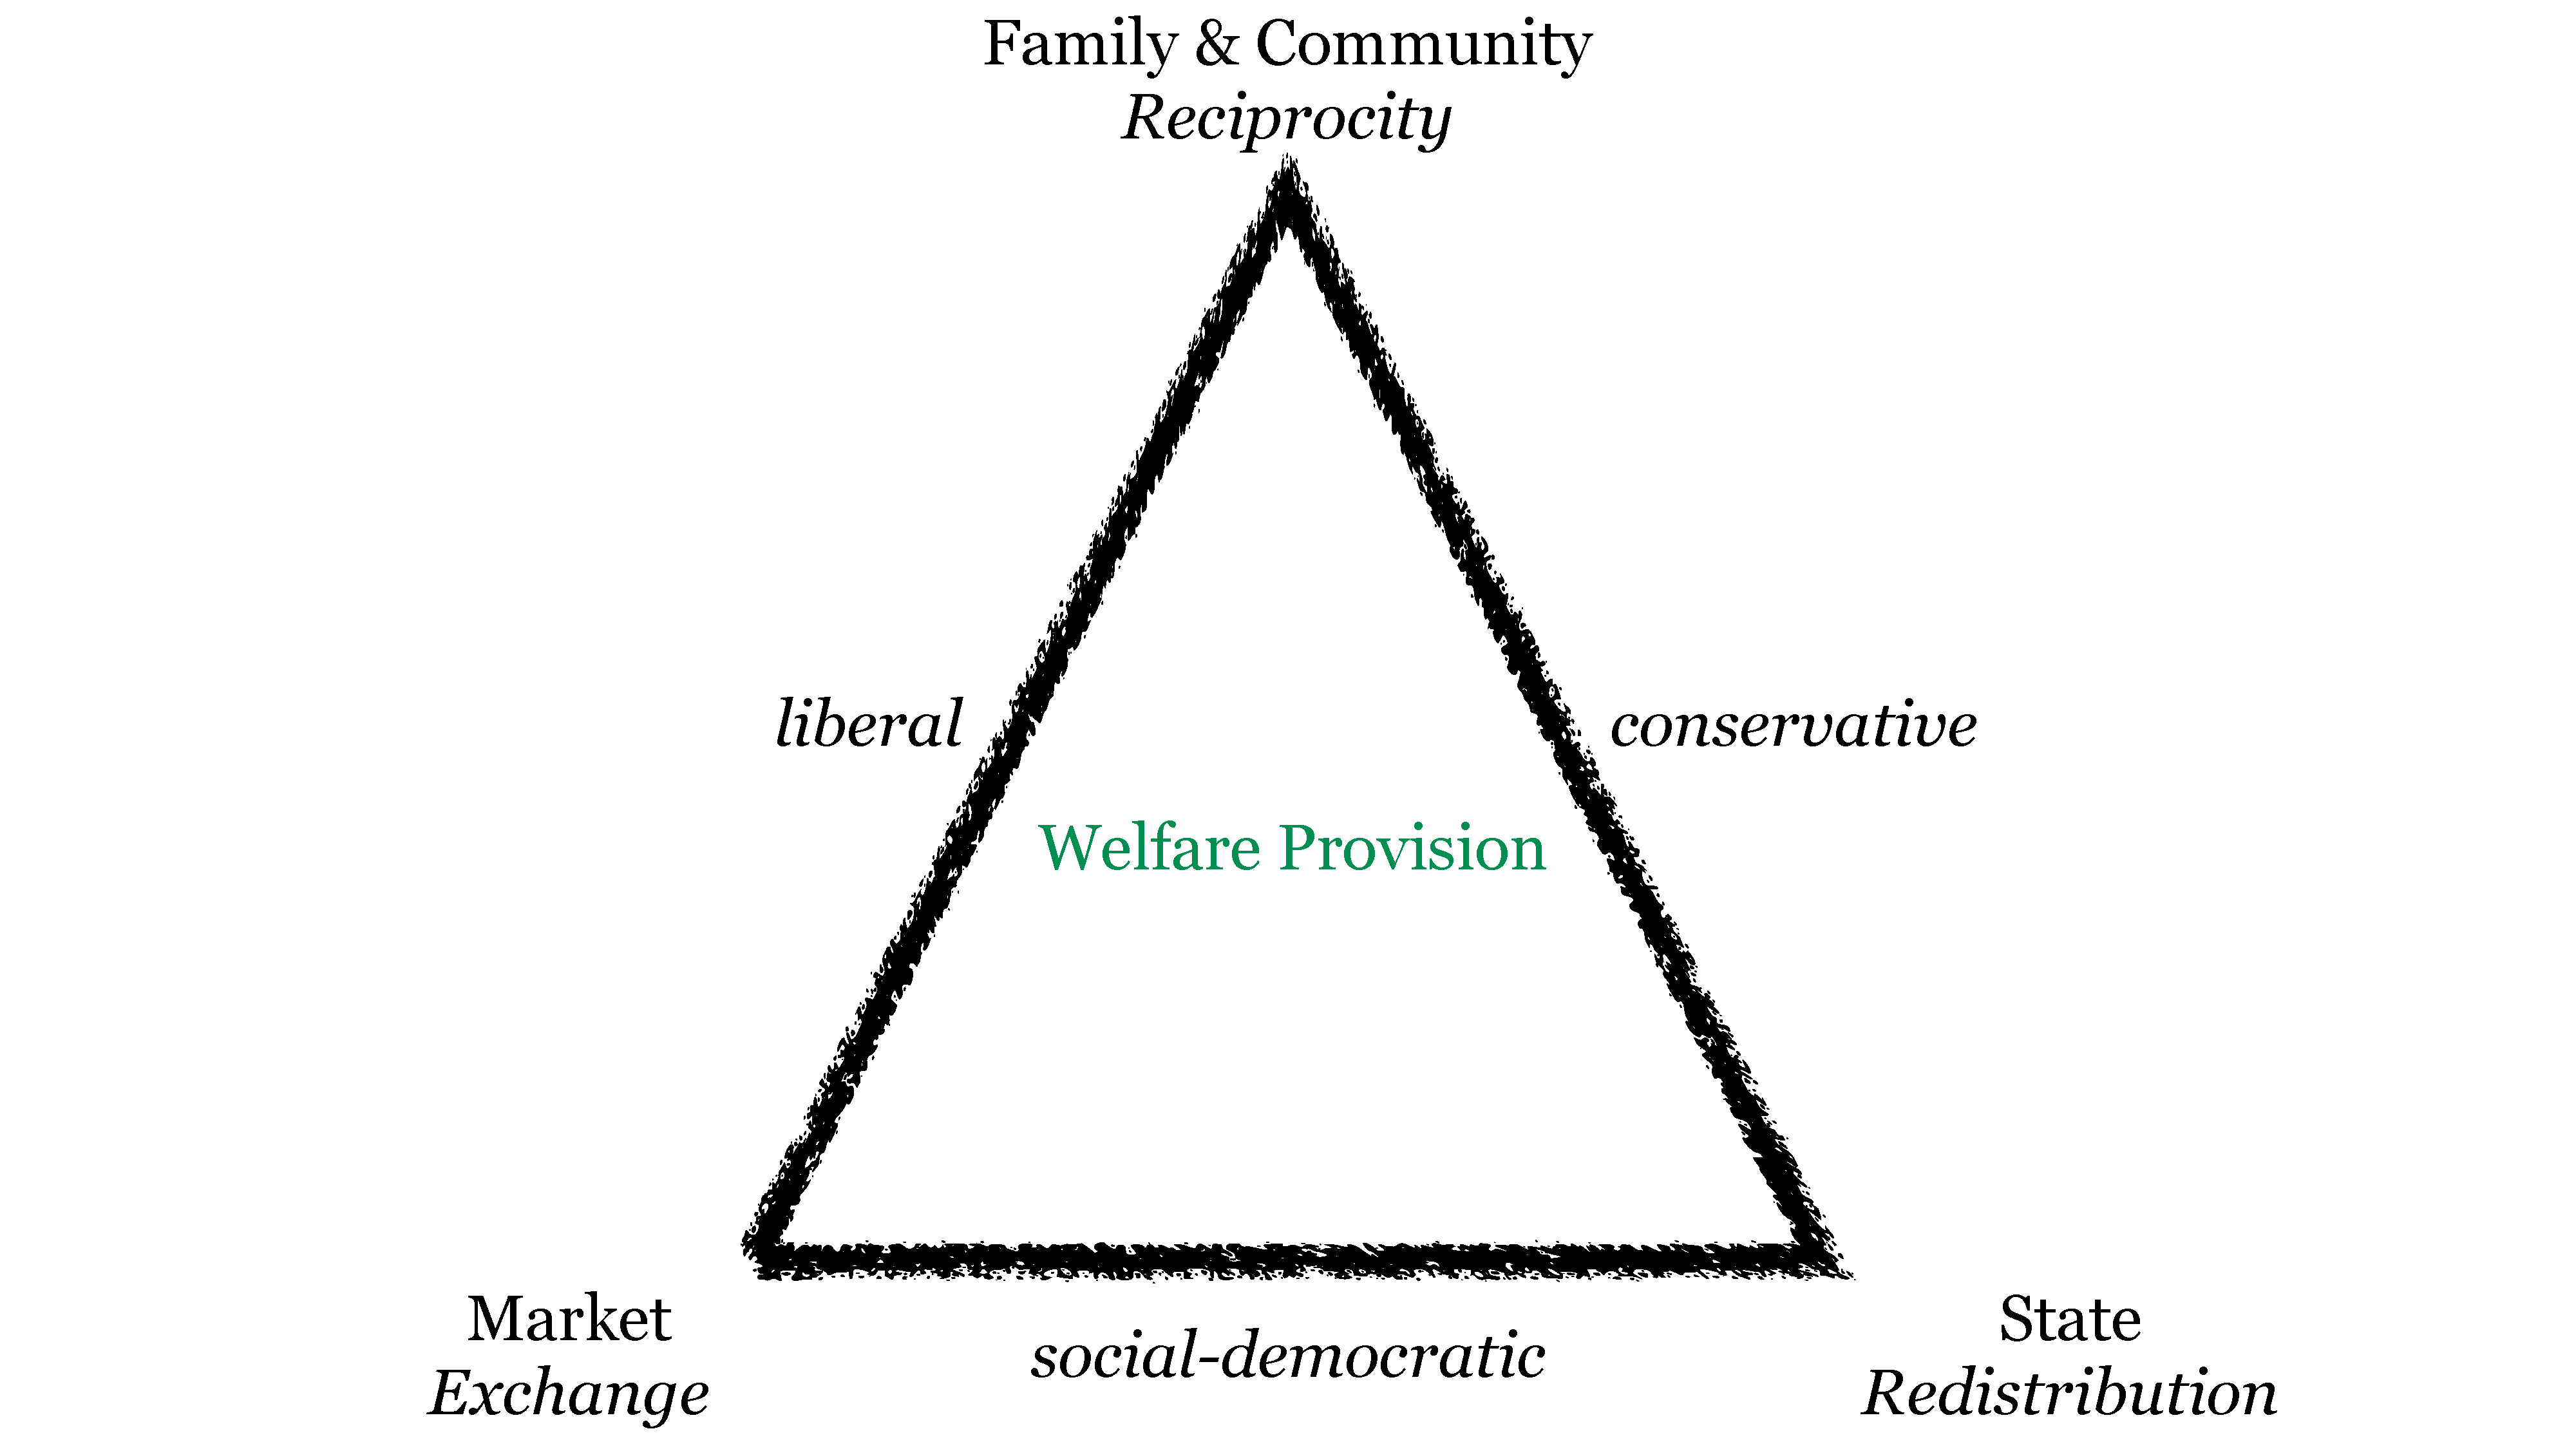
\includegraphics[width=1\linewidth]{ganssmann-welfare-provision}
	\caption{Welfare Provision and Political Ideologies}
	\label{fig:ganssmann-welfare-provision}
	\begin{flushleft}
		\scriptsize{Reproduced from \citet[334]{Ganssmann2010}}
	\end{flushleft}
\end{figure}

%here used to be the ppf-tax-regimes, it's now in testing-hypotheticals

%ganssmann is absolutely crucial for the constrained alternatives.

%Four disclaimers apply:

%\subparagraph{Not Original.} The perspective I take here is hardly original.
%Many others have, in greater width \citep{Stiglitz2002} or depth \citep{Sinn2004}, with narrower \citep{Scharpf1997} or different foci \citep{Zurn-2000-aa} discussed the first-order shortcomings of regional integration in the \gls{eu}, and economic liberalization elsewhere \citep{Stiglitz2002}.
%I aim here to reasonably comprehensively review the works of others and to restate some fairly conventional economic concepts in order to build a first-order checklist of welfare state design.
%I then discuss in \autoref{sec:Literature} how much of the \hyperref[sec:Literature]{current literature lacks awareness} of alternative, possible and desirable welfare states and why that matters.

%\subparagraph{No Positive Test.}

%why it matters, copied from the europe piece.
%add footnote

%McCaffery
	%our tax system is a disgrace, and has been so for decades.
%The way we tax is complicated, inefficient, and unfair.
%Yet whenever elected officials in Washington actually try to do something about tax, they tinker at best.
%At worst, they make the system even more annoying.
%We need fundamental, comprehensive tax reform, not ad hoc tinkering.
%Two, there is a widening gap between the rich and the not-rich in this country.
%It may surprise many readers to learn that there is a deep connection between these two facts.
%Tax as it is today is a cause of the wealth gap.
%Tax as it could be tomorrow would narrow it.
%That'sRead more at location 50   • Delete this highlight
	%Note:
%this is key.
%It's fucked up, but systematically so.
%Edit

%the below is from the europe piece, here comes th crisis of what happens when it doesn't work.

\subsection{Tax}
Taxation in the \gls{eu}, for the most part, remains an exclusive competence for \gls{ms}.
Under the acquis, only indirect taxes (VAT) are harmonized --- at ineffective, minimal levels --- with very limited cooperation in other fields (for example, \citealt{EuropeanCommission2009}, \citealt{TaxCoordinationandTaxCompetitionintheEuropeanUnion-EvaluatingtheCodeofConductonBusinessTaxation2001}).
Per its treaties, the \gls{eu} can harmonise only \emph{indirect}, always proportional taxes --- such as \gls{vat} --- and only by \emph{unanimous} decision of the Council on proposals by the Commission (Article 113, Treaty of Lisbon, 2009 / Article 93, Treaty Establishing the European Economic Community, 1957).
Union members do not even fully cooperate in collecting existing, national taxes:
instead of full reporting of all incomes, some incomes (for example, dividends) and some countries (for example, Luxembourg) are exempted and instead levy a proportional, much lower withholding tax.
It is, in short, no exaggeration to say that the \gls{eu} has no fiscal institutions or even coordination to speak of.

In the \gls{eu}, there is no match between the scope of economic activity --- the union-wide common market --- and the scope of taxation.

With no union-level taxation, what does this mismatch do to
\gls{ms}-level taxes?
As the abstractions of the mixed economy suggest, tax competition results.
For example, \cite{Genschel2009} find that tax competition is different and greater within the \gls{eu} than outside of it, and that it accelerates with time and enlargement.
\gls{eu} tax competition is a \gls{pd}, where states (strictly) dominantly prefer low taxes over high taxes and (Nash) equilibriate in suboptimal, mutual low taxation (\autoref{tab:EU-Tax-PD}, p.~\pageref{tab:EU-Tax-PD}).

%!TEX root=../tax-democracy-held.tex

\begin{table}
	\caption{International Tax Competition, Stylized as a Prisoner's Dilemma}
	\label{tab:Tax-PD} %change label?
	\begin{center}
	\begin{tabular}{m{1cm}m{2,3cm}m{2,3cm}m{2,3cm}m{2,3cm}}
		& & \multicolumn{2}{c}{\emph{Home}} \\
		& &Low Tax& High Tax\\ 
		\cline{3-4}
		\multicolumn{1}{c}{\multirow{4}{*}{\emph{Rest of World}}} & \multirow{2}{2,3cm}{Low Tax} & 		\multicolumn{1}{|r|}{3} & \multicolumn{1}{r|}{0}\\ 
		\multicolumn{1}{c}{} & \multicolumn{1}{c}{}& \multicolumn{1}{|l|}{3} & \multicolumn{1}{l|}{10}\\ 
		\cline{3-4}
		\multicolumn{1}{c}{} & \multirow{2}{2,3cm}{High Tax} & \multicolumn{1}{|r|}{10} & \multicolumn{1}{r|}{7}\\ 
		\multicolumn{1}{c}{} & \multicolumn{1}{c}{}& \multicolumn{1}{|l|}{0} & \multicolumn{1}{l|}{7}\\ 
		\cline{3-4}
	\end{tabular}
	\end{center}
	\scriptsize{\emph{Home} and \emph{Rest of World} are the only two countries. They set their tax rates either high, or low. Capital and other mobile factors flow to whichever country has the lower tax rate. Payoffs are state revenues.}
\end{table}

If, and to the extent that such a race-to-the-bottom is at play in the \gls{eu}, it will affect both levels and schedules of national taxation.

\paragraph{Levels.}
Straightforwardly, \gls{ms} will be strictly limited in the overall level of taxation they can sustain.
Governments will no longer be free to set a level of taxation, or, equivalently, determine the command-exchange components of the mixed economy.
In some cases, tax levels may even fall, as has been shown for \gls{cit} rates \citep{Piatkowski2008}.

%re-read Piatkowski about this stuff.

\paragraph{Base.}
Moreover, and more importantly, competition will also alter the base composition of taxation.
To avoid large \glspl{dwl}, as they should, governments will turn to bases that are relatively price inelastic, that is, economic transactions that cannot be altered to escape taxation.
\gls{eu} integration opens up a lot of new escape routes, especially for newly mobile capital, and, to a lesser extent, high-skilled labor:
they can relocate their economic activity to wherever the tax burden will be lowest.
This causes welfare-depressing distortions in the high-tax economy:
rather than face a now voluntary tax, these pareto-optimizing exchanges will not be made at all, and instead happen elsewhere.
For example, a rich entrepreneur otherwise willing to open a new factory in high income-tax Germany, may, faced with the new alternative of building the same facility in a low-tax location, forego his original plan.
Germany unambiguously looses welfare, both because the investment is not made, and also because it does not even generate any fiscal revenue.

Faced with these dynamics, governments will, again rightly so, shift their taxation to bases that are less prone to \glspl{dwl}, or equivalently, bases that are relatively less mobile.
Relatively less mobile bases in the \gls{eu} will be consumption and labor incomes, because consumers and workers cannot easily do their shopping and working in another country.

Other --- partly dysfunctional --- taxes traditionally used to raise revenue for mixed economies will be rolled back or falter altogether.
This applies especially to --- anyway defunct --- national \glspl{cit} that large corporations can often evade easily, in part because nailing down the locale of any particular increment of income of a multinational firm will always be conceptually difficult.
For example, the German holding of Deutsche Bank AG can easily reassign a particular income stream to a Luxembourg-based subsidiary, arguing that a crucial business process occurred there.
Tax administrations will always, and necessarily, be unable to argue where any particular value was created (\citealt{Ganghof2006}, \citealt{Ganghof}, \citealt[5]{Ganghof2007}).
Similarly, higher brackets of progressive \gls{pit} will also cause large \glspl{dwl} or, more likely and wisely, disappear, as high-income individuals change residence or citizenship, offshore their income-generation to other countries, or at least shelter it in foreign corporations no longer affected by high, backstop \glspl{cit}.
For example, a rich German entrepreneur can establish a new holding in Ireland to buy up his German-based firm, and have it retain most if not all of the earnings, effectively escaping german income taxation.

If and to the extent that Pigouvian taxes, or even fees fall on mobile bases, these will also either cause excessive market distortions, or, more likely, disappear.
For example, a German steel producer may, (hypothetically!) faced with the German ecotax, relocate to Poland, avoiding the higher energy price, \emph{without}, as the Pigouvian tax intended, raising the price of steel.
Overall energy intensity will remain the same, steel production will simply fall below equilibrium levels in Germany.

\paragraph{Schedule.}
Crucially, by shifting the base, \gls{eu} \gls{ms} will also alter the schedule of their tax regimes.
By relying more on taxing labor incomes, schedules will become more regressive:
most large incomes in developed capitalist economies are not labor, but capital incomes.
By relying more on (pre-paid) consumption and other indirect taxes, schedules will become regressive or --- at best --- proportional:
even if rich people, just as others, eventually spend all their income, they will only pay the same percentage in \gls{vat} or similar taxes.
If union member governments wish to avoid, as they should, excessive \glspl{dwl} they will have to sacrifice progressivity in tax.
The already impaired, but lone vestige of progression, the \gls{pit} together with its ugly, but necessary backstop,
\footnote{
	Personal income taxes on capital necessitate a corollary taxation of corporate income.
	Without it, taxpayers could easily evade payment by incorporating capital it in a firm, withdrawing earnings only slowly.
}
the \gls{cit} will either disappear altogether, or, largely equivalent, depress their schedules and degenerate into effective labor income taxes, with, at best, some residual but proportional taxation of capital.

\subsection{Dysfunctions}
	\label{sec:defunct}
What kind of an economic reality results from this open, but heterogeneous \gls{eu}, with unbounded trade, mis-configured currency union and rampant tax competition?
It is, and must be, a deeply dysfunctional design, boxing the European household in unattractive policy dilemmas, wasting its communal resources, ever building new imbalances, harboring new crises, and, ultimately, fracture the social contract.

\subsubsection{Underfunding}
	\label{sec:public-squalor}
Straightforwardly, the strictly limited revenues of \gls{eu} \gls{ms} confine them to structural underfunding, or at least, constrain the command-exchange \hyperref[sec:trade-offs]{trade-offs} that mixed economies are otherwise free to make (p.~\pageref{sec:trade-offs}).
%add reference.
By subjecting taxes to competition, any increment in more command production and distribution must be bought at an increasing price in lost economic activity, or \gls{dwl}.

In this scenario, governments rebalance their Haig-Simons identities --- as they always must --- by cutting public consumption or dissaving out of their wealth.
This can take many, but entirely equivalent forms.
For example, governments can save on public goods, such as road maintenance, or it can reduce transfer payments, such as welfare benefits.
It can also dig into its savings, and take on new debt, or, let infrastructure fall into disrepair.

Here, too, government is faced with unattractive choices:
to either cut public spending to suboptimal levels, to go into debt or to otherwise dissave.
%need evidence

\subsubsection{Unemployment}
The neoliberal agenda promised that if states cut their spending, at least their economies would greater economic growth.
Under a dysfunctional mixed economy, that is not necessarily so.
In the \gls{eu}, mixed economies cannot have the cake and eat it, they cannot even do one of the two.
Instead, its welfare states are faced with a twin crisis that is mutually reinforcing:
one of structural unemployment, and one of structural underfunding, as illustrated in \autoref{fig:twin-crisis} (p.~\pageref{fig:twin-crisis}).

Structural underfunding, aside from causing \hyperref[sec:public-squalor]{public squalor} (p.~\pageref{sec:public-squalor}), in the long run may also diminish the kind of public and common goods that drive future economic growth, such as basic research or infrastructure, and especially, education.
Over the long haul, structurally underfunded states will ill-equip workers for a global marketplace, and leave them with comparatively poor labor productivities.

In addition, structurally underfunded governments are increasingly unable to transfer  low- and middle-income workers, or, at least, exempt them from taxation.
In particular, the greater tax burden on immobile labor, and the constrained progressivity of tax under competition will make it even harder for workers to make ends meet at any given market income.
They have to pay more --- not less --- to the state, or, misleadingly named ``social insurance'' and keep even less for their personal consumption.

As a result, at least some workers will be relatively unproductive and face high taxes on their already low or middle market incomes.
If and to the extent that \gls{eu} welfare states maintain some minimum socially acceptable living standard, either through a minimum wage, or, equivalently, welfare transfers, these low and some middle income earners will find it increasingly difficult to earn enough on the market to meet this standard.
Any --- already diminished --- income will be further depressed by a tax wedge driven between the gross and net disposable incomes.
Both in a minimum wage, and a welfare transfer regime, those workers with productivities too low to make the minimum income on the market will exit the market, and collect welfare instead --- not out of laziness, but out of necessity.

The ensuing structural unemployment, in turn, reinforces the structural underfunding of the mixed economy government.
First, it creates greater needs for transfers, putting further strain on public transfers.
Secondly, it also depresses growth, and in the long run, diverges the economy from its long-term growth path, as segments of the labor force lie needlessly idle.

%here used to be \ref{fig:dual-crisis}, now only in 3-crises

Alternatively, of course, governments can lower effective price floors by cutting welfare benefits, minimum wages or by raising work requirements.
By lowering minimally acceptable social standards --- frequently euphemised as ``structural realignments'' or ``labor market flexibility'' --- states will have to abandon central welfare tenets and create and accept, once again, widespread working poverty.
%add some butterwegge results here.
That is, \gls{eu} welfare states can brake the vicious cycle of underfunding and unemployment if they cease to be welfare states, a configuration that \cite{Streeck2010c} has aptly called a ``permanent austerity regime''.
%visualize this already as an unattractive choice?

Governments of dysfunctional mixed economies, here, as always, are faced only with equally unattractive options:
to either save social standards at the price of structural unemployment and depressed growth, or to abandon them and risk widespread working poverty.

This dual crises, and the uneasy choices it forces, will only be exacerbated in a modern and open economy.
Modern economies already produce highly unequal returns, as winners take all and, equivalently, Baumols cost disease looms.
A modern economy will, by its very structure tend to produce people whose productivities are much lower than the overall productivity of their host countries.
%add hyperref.
Trade, migration and capital mobility add even more pressure.
As countries specialize even more according to their factor endowments (think:\ Romanian Nokia, German Management Consulting), remaining, relatively scarce factors (think:\ unskilled laborer in Germany) may find their market wages fall even further below the respective socially acceptable minimum income.
Especially rich states may then be forced to redistribute income to these individuals, but find themselves unable to raise the necessary revenues (progressively) without further reducing their competitiveness.

%need evidence

\subsubsection{Inequality}
Lacking any union-level fiscal institutions and marred by tax competition between the \gls{ms}, the \gls{eu} mixed economy lacks effective tools to redistribute market outcomes.
Both \emph{within} and/or \emph{between} member states, rampant inequality will remain unchecked, or even further widen.

At home, the mixed economy has lost its ability to dampen (possibly accelerating) winner-take-all dynamics, and to compensate the losers from trade and economic transformation.
\footnote{
	For example, \citeauthor{Beckfield2006} finds for the \gls{eu}-12 that nearly half of the rise in within-country inequality between 1973 and 1997 can be explained by regional integration \citeyearpar[979]{Beckfield2006}:
	inequality almost everywhere in the \gls{eu}, has been widening, at least in part due to regional integration \citep[for example,][265]{DaudUngl200}.
}
The great U-turn back towards more inequality, in Europe as elsewhere in the \gls{oecd} is well under way \citep{AldersonNielsen-2002-aa}.
As tax competition both erodes the base and depresses the progressivity of taxation, market allocations, increasingly, are final.
Moreover, structural underfunding and associated public squalor will also hit hardest the lower and middle income earners, further widening the divide in living standards.
Rich people can afford to exit from public provision, for example by paying doctors out of pocket, by sending their children to private schools or even walling their gardens and gating their communities.
Lower and middle income earners have no such exit option, but are stuck with decrepit public provision.
%need evidence

Between \gls{ms}, too, inequality will remain unchecked, as member and union level governments have no instruments to alter distributive dynamics of trade, that may --- or may not --- lead to fast convergence of productivities, and related, living standards.
What is worse, the poorer mixed economies are especially constrained:
at low productivities, they can least afford to burden mobile capital, and other mobile, high-earning factors, such as professionals with any, let alone progressive taxation.
With open borders, but without coordinated tax or union-level transfers, these poorer \gls{ms} currently can only take the hard, unmitigated route to economic convergence:
they tax mostly (low-productivity) labor, proportionally if not regressively, and at low overall public spending levels \citep[for example,][267]{DaudUngl2008}.
By contrast, in the higher-productivity, rich \gls{ms}, corporatist arrangements, strong trade unions and substantial, if increasingly dysfunctional welfare regimes can still eek out pockets with sometimes generous welfare provision:
in always capital-intensive, often high-value add and sometimes oligopolistic --- not commodity ---production, these economies can, at least in some sectors, afford welfare.
For example, a Bavarian specialist engine builder with high capital and relatively low labor inputs and maybe a handful competitors on the world market,  may, faced with strong unions, accept above-equilibrium, possibly efficiency wages.
Not so in Romanian manufacturing:
Producing low-margin commodities, with little capital but hundreds of competitors and easy access, firms have to compete tooth-and-nail on labor costs.
And so, \gls{ms} may not only fail to converge as quickly, or as closely as they could, or hoped to, but the very \emph{conditions} for economic development will diverge widely.
The rich, high-productivity \gls{ms} can still, if inefficiently and incompletely, dampen and distribute the pain of whichever economic shock hits or transformation sets in.
In the poor, low-productivity East and South, it will be bare-bones laiss\'{e}z-faire capitalisms.
\footnote{
	\citeauthor[25]{Galbraith2002a} precisely describes an analogous, worldwide dynamic:

	\begin{quote}
		\emph{``In sum, it is not increasing trade \emph{as such} that we should fear.
		Nor is technolocy the culprit.
		To focus on `globalization' as such misstates the issue.
		The problem is a process of integration carried out since at least 1980 under circumstances of unsustainable finance, in which wealth has flowed upwards from the poor countries to the rich, and mainly to the upper financial strata of the richest countries.
		In the course of these events, progress toward tolerable levels of inequality and sustainable development virtually stopped.
		Neocolonial patterns of center-periphery dependence, and of debt peonage, were reestablished, but without the slightest assumption of responsibility by the rich countries for the fate of the poor.
		It has been, it would appear, a perfect crime.
		And while statistical forensics can play a small role in pointing this out, no mechanism to reverse the policy exists, still less any that might repair the damage.
		The developed countries have abandoned the pretense of attempting to foster development in the world at large, preferring to substitute the rhetoric of ungoverned markets for the hard work of stabilizing regulation.
		The prognosis is grim:
		a descent into apathy, despair, disease, ecological disaster, and wars of separatism and survival in many of the poorest parts of the world.
		Unless, of course, the wise spirits of Kuznets and Keynes can be summoned back to life, to deal more constructively with the appalling disorder of the past twenty years.''}
		\\*
		--- John K.\ \citet[25]{Galbraith2002a}
		%is that the right Galbraith?
	\end{quote}
}

In the \gls{eu}, Kuznet's and Keynes' grand hopes, that welfare would --- and should --- always follow growth, are dashed (as cited in \cite[22]{Galbraith2002a}.
If they have any choice at all, it is a very unattractive one for the governments of the union:
they can either stay in the common market and reap the gains from trade and abandon all or some welfare, \emph{or} they can exit the union, stall economic integration, save their welfare regimes and retreat to autarky and recession.

\subsubsection{Imbalances and Crises}
	\label{sec:imbalances}

\begin{verse}
	\href{http://www.npr.org/blogs/money/2012/03/01/147720368/50-ways-to-leave-your-lender}{50 Ways to Leave Your Lender}

	The problem is all inside your head, she said to me,\\
	You can't pay back 200 percent of GDP,\\
	You have to negotiate, if you want your country free,\\
	There must be 50 ways to leave your lender.

	You really don't want the IMF to intrude,\\
	Furthermore, they'll force austerity for the interest that's accrued,\\
	Imagine your middle class, subsisting on cat food,\\
	There must be 50 ways to leave your lender.\\
	Fifty ways to leave your lender.

	You just stretch out the loan, Joan,\\
	Cut the creditors' hair, Claire,\\
	Or boost GDP, Lee,\\
	Just listen to me.

	Print more money, honey.\\
	No need to pay back, Jack!\\
	Structure a default, Walt.\\
	And get yourself free.\\
	--- Planet Money / National Public Radio, 2012
\end{verse}

Democratic governments, firms and households alike will be under great strain from the underfunding, unemployment and inequality that a dysfunctional mixed economy creates.
%add hrefs.
They may take on any possibility to temporarily relief the pressure they are under, even if it will not solve, or even exacerbate the situation in the long run:
here, too, humans and the institutions they man, suffer from time inconsistency.

In modern financial capitalism and complex societies, there are some powerful painkillers to numb the effects of a dysfunctional mixed economies.
As painkillers go, they treat the symptoms, not the disease, and have serious side effects.
And so it is with the macroeconomic temptations in the \gls{eu}:
as powerful drugs, they seemingly let economies transcend their material means, spread euphoria and frenzy.
Only their cure is, ultimately, delusional, their treatment addictive.
While under the charm of such chimerical boom and prosperity, economies keep building pressures and imbalances, that, one day, will unload in financial shocks and systemic crises, that, if sufficiently large, can disturb or bring down entire markets.
After this kind of ecstasy always comes a day of reckoning, with a catastrophic hangover.

Just when an economy is in such drug-enduced delusion, and living beyond its long-term growth path is, as always in uncertain markets, hard to tell.
National balance of payments accounts provide as in \autoref{fig:BoP} (p.~\pageref{fig:BoP}) an intuitive, if rough-and-dirty first indication.
Between economies, too, an identity akin to Haig-Simons and the conservation of matter, holds:
for any good or service that leaves the country, there must ultimately be imports of equal value, or, a change in ownership of foreign assets, that is, the promise of \emph{future} imports of goods and services.
Conversely, any import must be matched by exports of equal value or it will be offset in \emph{foreign} ownership of domestic assets, that is, claims against future domestic production.
As all the most important economic abstractions, this one is simple:
balance of payments accounts are double-entry bookkeeping, only at the economy level.

The components of balance of payments accounts, as the Haig-Simons identity, break down over households, firms and governments.
For example, in a fictions German account, households can import olive, or firms can import particle filters as semi-manufactured inputs, or governments can import commuter trains for public transportation (\autoref{fig:BoP}, p.~\pageref{fig:BoP}).
In these accounts too, positions of one owner are offset by positions of other owners in the same economy.
For example, German household exports of home-made cuckoo clocks can be offset by said firm imports of particle filters in a roundabout way, when clockmakers buy French-particle-equipped German cars, or following some other chain of exchanges.
Positions  also offset across the equality sign.
For example, German household imports of olive oil may be offset by government issues of German bonds to Greek oil producers, with the government channeling the revenue to oil-consuming welfare recipients, or through a myriad of other transfers.

\begin{figure}[htbp]
	\begin{center}
	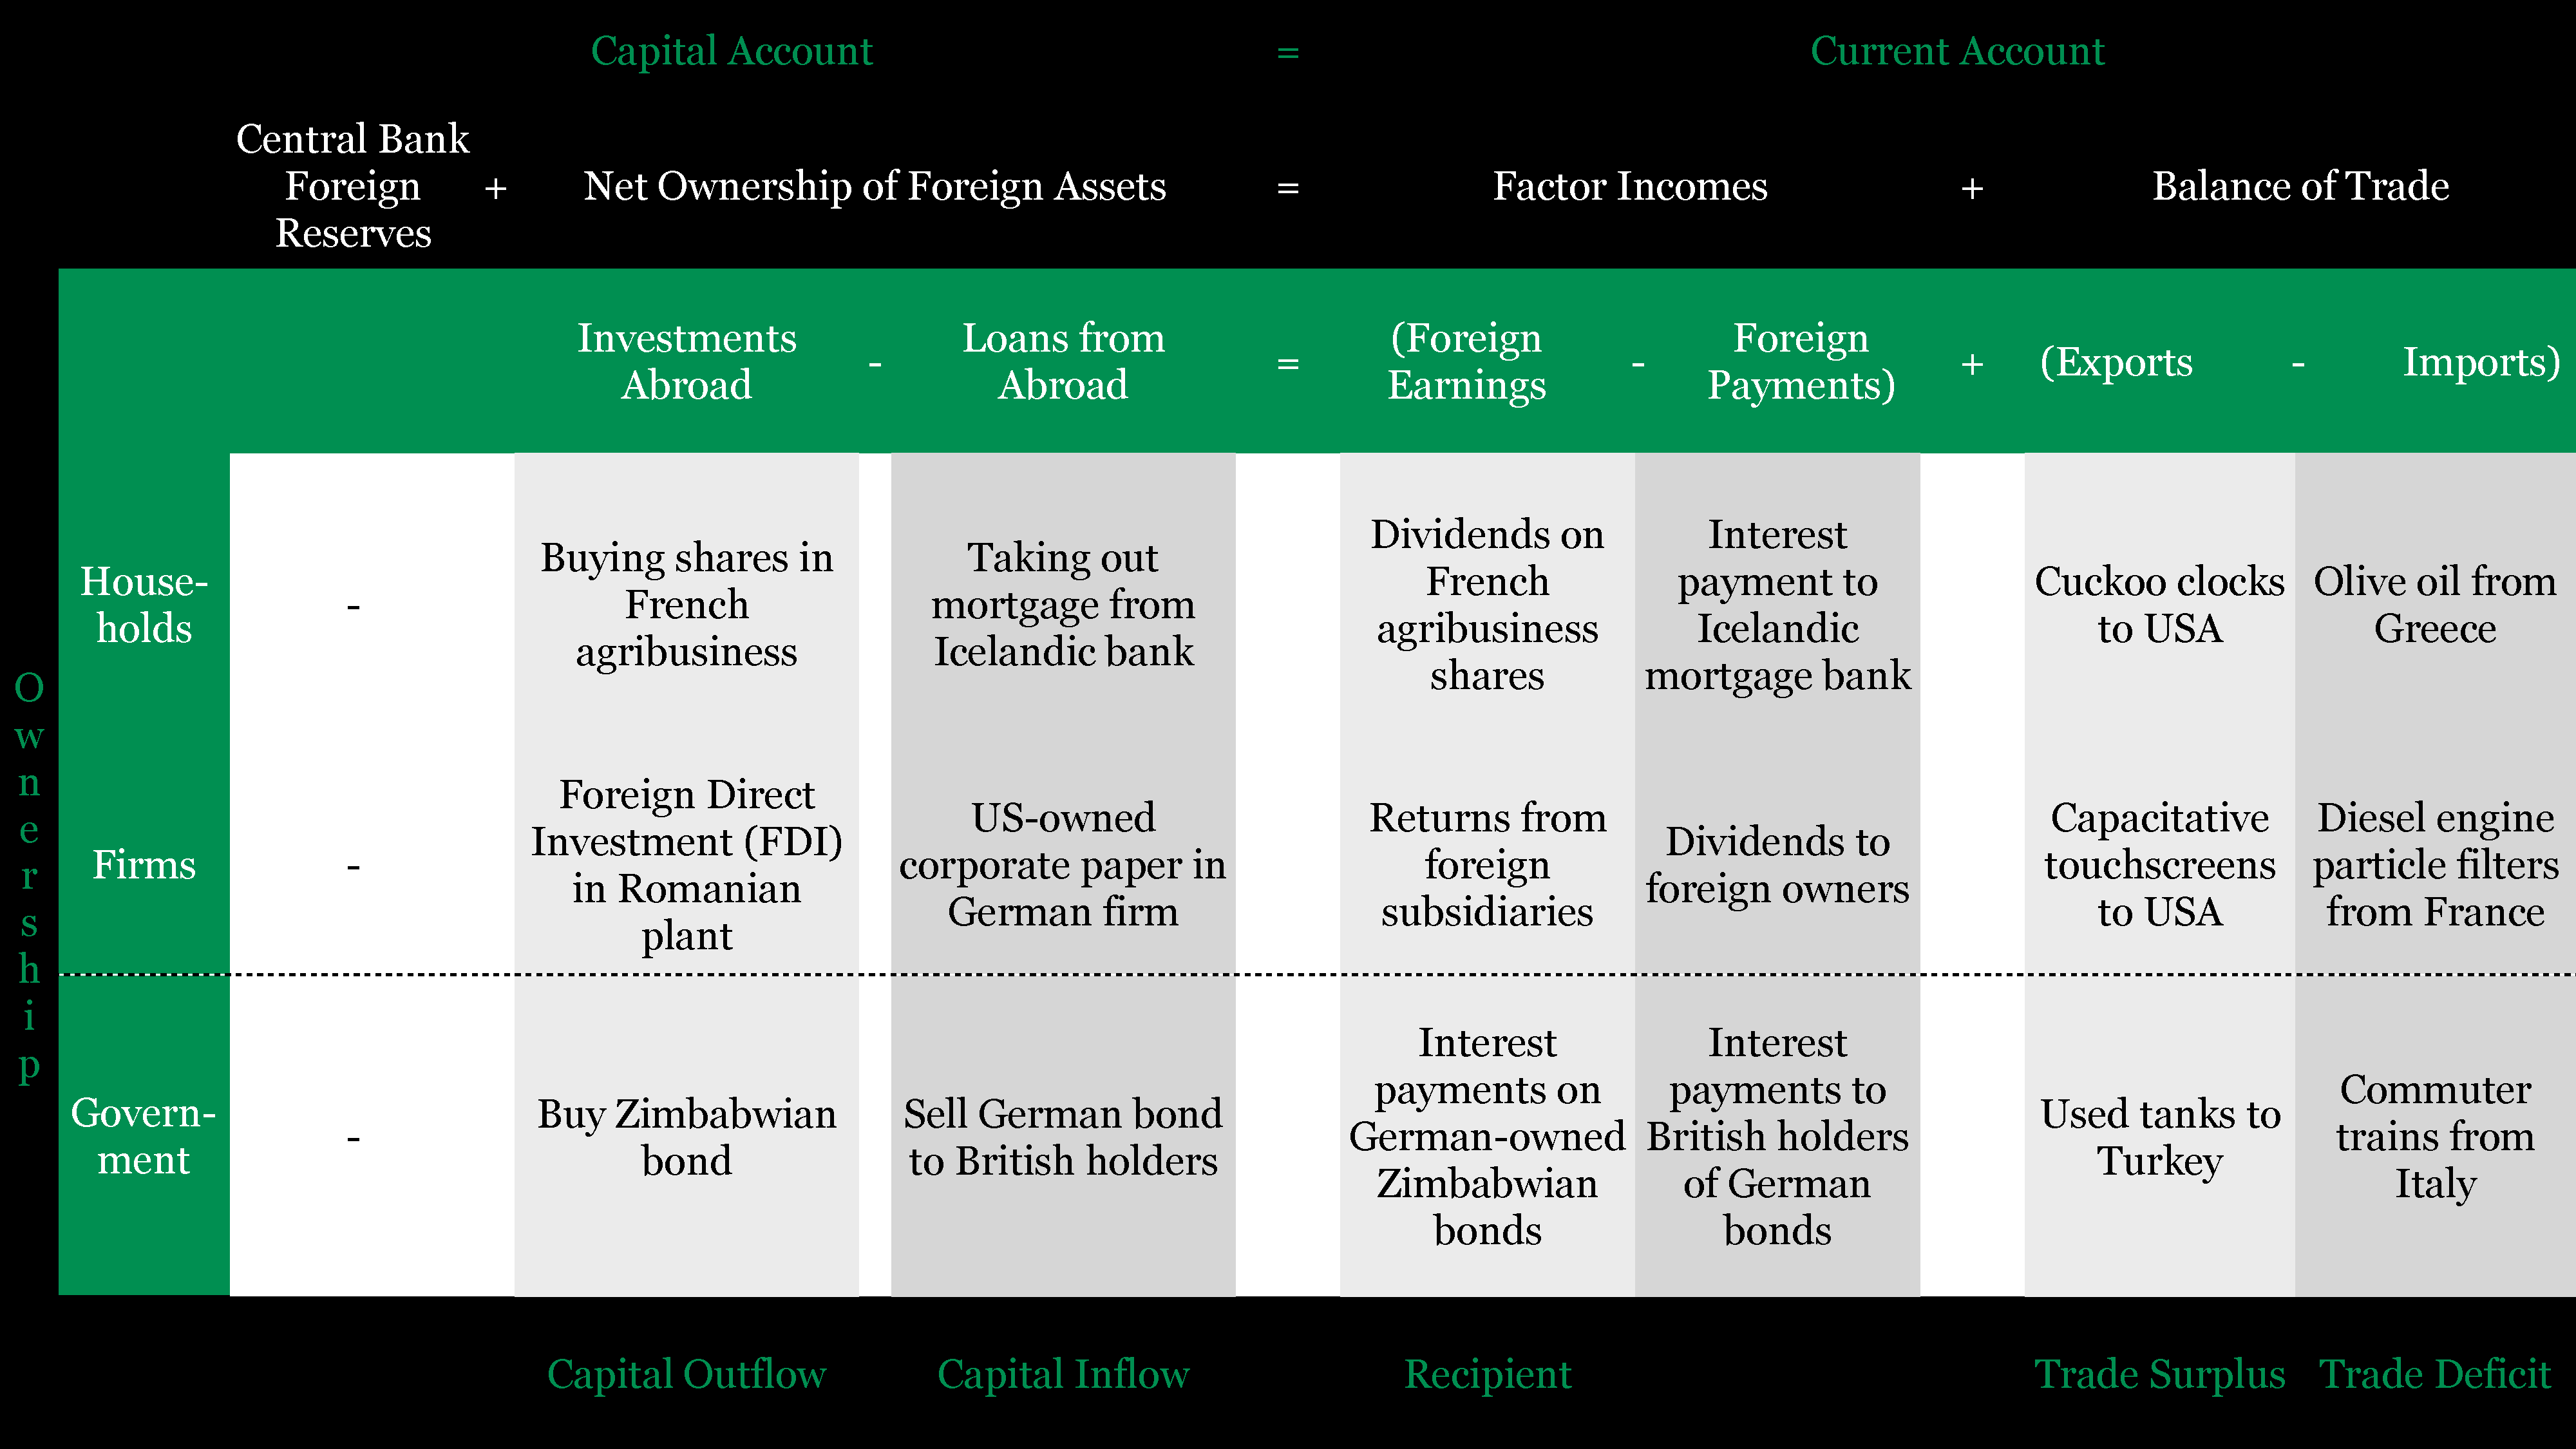
\includegraphics[width=1\textwidth]{balance-of-payments}
	\caption{A (German) Balance of Payment Account with Examples}
	\label{fig:balance-of-payments}
	\end{center}
\end{figure}

Balance of Payment accounts are easily misunderstood or oversold, for a four reasons:
\begin{enumerate}
	\item Trade deficits and surpluses between any pair of countries are frequently reported, but meaningless and entirely unproblematic, just as shoppers need not worry about a trade deficit with the local supermarket.
	Trade deficits --- as consumer debt --- are potentially worrying only if they are \emph{net} of all exchanges with all trading partners.

	\item Conversely, balance of payments accounts do not apply  only between countries, as is easily assumed, but is, in fact a meaningful and true identity between any group of market participants and the rest of their trading partners, all the way down from nations to households.
	For example, a trade deficit may also arise between laggard regions, impoverished demographics or even generations, and the rest of an economy, with much the same possible problems.

	\item In the short term, even such trade deficits may not be problematic, but, in fact, help to stabilize economies from exogenous shocks.
	%reference OCA argument

	\item Even in the medium and long run, persistent trade deficits may be ok if and to the extent that the resultant capital inflows can reasonably be expected to currently, or in the future, earn whichever factor income was promised.
	For example, emerging economies may well experience persistent trade deficits for some time, while machinery is imported to equip the workforce, if and to the extent that the resulting, now capital-deepened production pays off as expected.
\end{enumerate}

Still, balance of payments accounts are an immensely enlightening abstraction, without which trading mixed economies cannot be well understood:

\begin{enumerate}
	\item Trade deficits are not a sufficient, but still a necessary condition for building macroeconomic imbalances.
	Not every trade deficit will betray an economy living beyond its means, but every economy artificially held above its long-term growth path by said financial drugs \emph{will} leave a grave trade deficit in its wake.

	\item The balance of payments identity shows, as Keynes  argued forcefully, if somewhat ineffectively at the Bretton-Woods conference in 1944, that these macroeconomic imbalances know no \emph{one} culprit.
	The loaded language notwithstanding, both deficit \emph{and} surplus economies are, equally, at fault.
	One parties excessive imports are another parties dumping exports.
	To get to equilibrium, where imports equal exports, either of the two parties, or both, must change its prices.
	To pride oneself, as German leaders frequently do, in being an export champion --- but not an import champion --- is but a mindless return to the folly of beggar-thy-neighbor, and, before that, mercantilism.

	\item Financial flows always track flows of tangible goods and services, as well as vice versa.

	\item It does not much matter \emph{who} --- households, firms or government --- in an economy creates the trade deficit.
	Only the deficit net of all economic actors in a given region matters.
\end{enumerate}

How, then, do we know the acceptable trade deficits, from the unsustainable ones?
We look at the offsetting changes in the capital account, and check whether these are intertemporally efficient, or whether they were enabled by failed markets.
In the \gls{eu}, as in any other mixed economy, we must beware of these smoke and mirrors, that only forestall and worsen the inevitable day of reckoning:
credit bubbles, asset bubbles, inflationary pressure, and nominally invisible, but real dissavings.
 %add hrefs.

\begin{description}
	\item[Credit Bubbles \& Default.]  Trade deficits can precipitate in capital inflow, as new foreign-held debt.
	To receive their extra imports, deficit economies issue different forms of IOUs, including government bonds, corporate debt and household credit, sometimes backed by physical collateral, as in a mortgage.
	%gls IOU

	If the sum of these debts, is sound, so is the trade deficit.
	If debts, sour, or were overly optimist to begin with, the trade deficits cannot stand.
	Consider the two scenarios:
	\begin{enumerate}
		\item The loans are performing as long as, if, and to the extent that whichever projects they financed generate sufficient earnings to pay back interest and principal.
		For example, if the extra, imported surplus production the IOUs enabled were transformed into a competitive factory that now churns out export merchandise, the loan can be paid be back out of these exports and revenues.

		In the \gls{BoP}, the initial trade deficit is first offset by the loaned capital inflow, which later flows out again as the loan amortizes, offset by foreign factor payments and exports of the produced merchandise.
		In effect, the loan has, as efficient credit should, inter-temporally balanced past trade deficits with future trade surpluses and/or foreign payments.
		It matters little whether, and in which proportion the amortization on the capital account is offset by either foreign payments or equivalent actual exports, and whether the factory's merchandise is actually for export or domestic consumption.
		In the balance of all economic transformations and exchanges, successful factories and other projects can always honor their loans \emph{without} curtailing the living standard of the population.
		Interest, and maybe even collateral, are paid back out of \emph{extra} production that would not have otherwise occurred.
		We need not worry about this kind of trade deficit:
		because it moves everyone closer to the long-term growth path, is an inter-temporal Pareto, or at least Kaldor-Hicks optimization.

		\item The loan goes bad as soon as, if, and to the extent that whichever projects they financed do not generate sufficient earnings to pay back interest and principal.
		For example, if the factory is not competitive, or --- more to the european point --- no one needs or can afford the airports, malls and mansions into which the extra imports were coagulated, there are no revenues or exports to pay back the loan.
		In the extreme, but conceptually similar and now plausible case, the extra imports were not meaningfully coagulated into capital at all, but were simply consumed away at present.

		Come the day of inevitable reckoning, the deficit economies have two choices:

		\begin{enumerate}
			\item If the loan in question carries effective recourse, the deficit economy has to return the loaned capital in other, \emph{material} ways.
			As when a leasing company repossesses a car on which payment the lessee has fallen behind, deficit countries must return the surplus production in some form.
			For example, the deficit economy may ship back the foreign-financed machinery in the project, or, more likely, return the same amount of surplus production transformed into some other good or service.

			This is the hard way of rebalancing the \gls{BoP}:
			the inevitable, promised outflow of capital on the capital account (reflecting net changes in the ownership of, but not generation of, assets) can be balanced only with an often painful trade \emph{surplus}, because there are no factor incomes to be otherwise offset on the current account, reflecting a nation's income.
			Either way, a failed investment enforces a later, and often painful trade surplus to return principal and return.
			%work in these definitions more smoothly

			\item Alternatively, if and to the extent that debtor economies (can) forego recourse and exert sovereignty vis-a-vis creditor economies, they (partially) default on their commitments and simply refuse to return the coagulated surplus production.
			In that case, creditors are stuck with their claim.
			By fiat, the original loans become full, or partial \emph{transfers} from the debtor to the creditor economies.
			Here as always, the two sides of the \gls{BoP} identity cancel out:
			the original trade deficit is matched by a later, ex-post, enforced, foreign payment in the form of debt forgiveness, haircut or default.
		\end{enumerate}

		No matter the choice, this kind of trade deficit is never an optimization, but an unavoidable \emph{redistribution}, either from surplus future to deficit present if and to the extent that debtors pay, or from creditors to debtors, if and to the extent that debtors default.

		Crucially, it matters very little who in the deficit economy --- households, firms or government --- initially took on debt.
		These non-performing loans will redistribute from future to present, or creditor to debtor no matter who signed them.
		In many cases, government will be forced to act as the lender of last resort and take on, or guarantee all the bad loans, both to counteract adverse selection and, often to save an exposed banking system from systemic crash.
		Even if and to the extent that government, or, equivalently, future taxpayers, can avoid to take on the bad loans, the redistribution is merely concentrated on whoever remains nominal debtor.
		Domestic policy can force only \emph{some} people --- ideally those responsible --- to repay, but, short of default --- another redistribution --- it cannot void the need to repay.
		Here, as always, something akin to economic conservation of matter reigns:
		when credit bubbles burst, someone will have to pay back the future, either some debtors, all taxpayers, some creditors, or any combination thereof.

		In addition to these mere inter-temporal distributions, credit bubbles and associated mass defaults or austerity, of course, also waste economic welfare, because of the turmoil they harbor, not to mention the hardship they imply.
		As the business cycle fluctuates wildly in such crises, the economy diverts from the long-term growth path, leaving resources either depressively idle, or manically scarce.

		Credit bubbles are a market failure that may plague any economy --- not just the \gls{eu} --- but the european, defunct mixed economy is particular prone to them, for at least three reasons:

		\begin{enumerate}
			\item The \gls{eu}, until at least 2012, exercised most macroprudential oversight and otherwise mostly regulated financial markets at the \gls{ms} level.
			Here, even the regulatory arm of the mixed economy was impaired, and regulations might have been arbitraged to suboptimal levels.
			%find source.

			\item Monetary policy drives bank lending.
			The \gls{ecb}, because it can set only \emph{one} monetary policy, was unable to react to credit bubbles in individual markets or regions, such as Spain or Greece.

			\item Equivalently, if there were in the \gls{emu}, or ever hoped to meet the its nominal convergence criteria, deficit and credit-crazed \gls{ms} also could not devalue their currency through monetary interventions.
		\end{enumerate}
	\end{enumerate}

	\item[Asset Bubbles \& Crashes.]
	Broadly similar, and often concomitant to credit bubbles, asset bubbles can also fuel trade deficits.
	As some assets in the deficit economy are persistently overvalued, foreign investors buy up these domestic assets, offsetting the trade deficit on the current account with a capital inflow on the capital account.
	Real estate, stock or some other asset that did not previously exist, or belonged to domestic investors, changes hand to foreign investors, expecting an ex-post unreasonable return.
	Come the day of reckoning, asset prices plunge, and much the same process sets in as when credit bubbles burst, only in asset bubbles, the default incidence is on the foreign investor, because she will usually, if not always, have taken risk-bearing equity in the asset.

	Asset bubbles, too, are a redistribution from a future day of reckoning to a manic present, and, in that future, a redistribution from foreign investors to the domestic economy.
	In addition, asset bubbles also waste welfare:
	when they burst, they spiral downwards, often cause grave systemic risk and generally divert the economy from the long-term growth path.

	Asset bubbles, too, are a universally looming market failure, but the \gls{eu} is particularly vulnerable, again, because of likely regulatory arbitrage and ill-fitting monetary responses to local business cycles.%add href.

	\item[Monetary Expansion \& Inflation]
	Overly expansive monetary policy can also enable unsustainable trade deficits.
	In this scenario, central banks simply inject more fiat money into the economy to offset the current account deficit with a Potemkin inflow of capital.
	Fiat money, of course, never creates capital, and if, when and to the extent that this bluff is called, inflation ensues:
	money supply and demand equilibrate at new, higher price levels.

	This problem is widespread in the \gls{emu} with asynchronous business cycles, a single interest rate target and no transferred stimulus to speak of.
	In those regions where a low interest rate pumped too much money into the economy, as now appears to have been the case in Ireland, Spain, Portugal and Greece preceding the 2008ff crisis, loose money silently credit and asset bubbles, and might have already built yet-to appear inflationary expectations.
	%I really don't know what I'm talking about, here
	%Need data.

	Inflation, here, as always, wastes resources and redistributes arbitrarily.
	%add /href.
	The middle class and older people, with frequently nominal denominated assets (pensions), but real denominated liabilities (rents) will be particularly vulnerable to whichever level of inflation this crisis might, eventually, bring.

	Inflation, too, as the other temporary diversions from the long-term growth path, redistributes from the future to the present.
	Even inflation does not spiral to double-digits or more, \emph{any} additional increment in medium-term inflation and expectations is costly, as disinflating to previous levels is painful and often causes prolonged unemployment.
	%add source.
	%reference 70s disinflation

	\item[Dissaving \& Depletion]
	Trivially, economies can also go into unsustainable  trade deficits by real dissaving.
	Instead of, say, selling shares in domestic companies, the deficit economy can just burn more of strictly limited fossil carbon, diminishing its real, if not its nominal assets.

	Because such real assets, including an economies infrastructure, demography, environment or CO2e levels as unresolved commons have no defined ownership rights, they do not nominally show up in the capital account of an economy.
	Whatever this assets are transformed into, however, may well show up as an export in the current account.
	For example, a deficit economy can dig into its coal and iron ore resources, transform them, and export them as steel, offsetting other imports.
	Because the dissaving in natural resources is not usually recored, and thus triggers no change in the capital account, the steel export revenue will erroneously be attributed as a domestic \emph{income} in full, when in truth, much of the revenue comes from dissaved domestic assets, that ought to be recorded on the capital account.

	Such dissavings --- by definition --- redistribute from the future to the present.
	As dissaving most easily and nominally invisible occurs out of vulnerable commons, it also wastes the welfare of some of our most precious, communal resources.
	If, when and to the extent that they are depleted to sustain trade deficits, we may never or only at great cost be able to restore them.
	%might need to strengthen the crisis and imbalances components in the above.
\end{description}

I cannot marshall evidence here to show how each of these dynamics caused the 2008ff Euro, let alone the broader sovereign debt crisis.
Nor can anyone, in 2012, reliably predict which of imbalances may yet turn out to be unsustainable, and why.
What I do claim here is that whatever the actual imbalances and crises of the embattled \gls{emu} and \gls{eu} are, or will be, they will, underneath it all, follow these scripts.
Using some economic imagination, \emph{these} are imbalances and resulting periodic crises we would expect to plague any such internally open, but dysfunctional mixed economy.

While this european mixed economy may be of its own kind, the market failures that enable these imbalances and trigger the resulting crises are in no way \emph{sui generis}.
The herding and information externalities that inflate asset and credit bubbles, the systemic chain-reactions that loom on large defaults and the tragic commons depleted by real dissavings are the kind of market failures that plague all real-existing capitalism.
As such, they must be meet the appropriate regulatory, fiscal, and --- to a lesser extent --- monetary responses.
 %add \href
Similarly, loose money tempts governments of all market economies, not just --- in fact, probably, least of all --- in the \gls{eu}.
It, too, must everywhere be curtailed by policy:
a constitutionally-enshrined monetary governance, preferably a robustly independent central bank, bound to a well-defined goal.
Because as dangerous drugs endemic to capitalism, these problems are not European problems, they also do not require a European solution.

Still, the deficient european acquis exacerbates the imbalances and crises looming everywhere, in at least three ways (\citep[echoed by][25]{Bordo2011}):

\begin{enumerate}
	\item Without a monetary union or nominal convergence criteria thereto, trading economies can intervene in their exchange rate, or, at least, let their currencies depreciate freely.
	As adjustment mechanisms, none is as fast as currency devaluation to get out of trade deficits.
	In an instant, imports become more expensive and exports become cheaper, ideally, until import and exports equilibrate at the free exchange rate.
	Alternative --- and ultimately equivalent --- domestic readjustment of (higher) prices and (lower) wages often takes longer, maybe too long to avert a \gls{BoP} crisis.

	Discretionary exchange rate interventions are difficult to get right, and easily deteriorate into competitive devaluation, or beggar-thy-neighbor by a fancy name.
	%add source.
	Freely fluctuating exchange rates, in turn, are costly as the second theory of optimal currency areas reminds us, %add source
	and they, too, might be the result of herding or otherwise failing global currency markets.

	As drug addiction therapies goes, the methadone of devaluation is, at best, a mixed blessing.

	And still, it is a prescription, the european economy has to do without, no matter the indication.
	Within the \gls{emu}, everyone in the \gls{eu} who ever wants to join, currencies cannot fluctuate.
	To readjust, member economies can only hope their wages will not be too downwardly sticky.

	\item Creditors and debtors alike will anticipate the systemic risk and spillovers that the monetary union bestows on all its members.
	They know that other members too, would suffer from defaults or, related, \gls{emu}-exit, and, therefore, will likely bail them out.
	%add more stuff here, why is that so?
	%I wrote that somewhere.
	With systemic default risk as a union-level commons, but decisions in individuals, firms and, at best, \gls{ms}-hands, credit everywhere, but particularly in the high-risk economies, will be too loose.

	The \gls{eu}, in other, metaphorical words, is not only plagued by powerful and addictive drugs, but dealers and addicts alike can reasonably expect to be saved --- as the should --- if they overdose.

	\item Lastly, and familiarly, the european mixed economy lacks the fiscal means to otherwise rebalance internal demand, that intact mixed economies use to mitigate regional imbalances, including public works, industrial policy, or even straightforward transfers.
\end{enumerate}

The imbalances that have built up over the last years of European integration, and the crises in which they now seem to erupt, tell of the market failures of our capitalist economy.
But they also betray the underlying dysfunctions and unfairness of an impotent mixed economy, that built these pressures in the first place.
To bemoan only the market failure, and to seek to redress it is as naive as it is dishonest.
Even worse, to simply wish away the crises, and to blame someone (``the banks'') --- \emph{anyone} (``'the markets'') for our misfortune, is to shoot the messenger, rather then to heed her warning.

In drug policy, if you are faced with a rampant substance abuse, you have to follow \cite{Mills-1959-aa}, and sociologically re-imagine the saddening observation of an overdosed corpse:
you have to ask how, and why, people socially turn to harmful drugs in the first place, and then, if you can, cure this anomie, whatever it may be.
If you only wage a war on drugs, they will always win.

And so it is with the imbalances and crises facing the \gls{eu} today:
we have to use our economic imagination to explain how, and why, the european economies turned to delusional market failures in the first place, and, if we can, strengthen them to resist any siren call.

Our anomie, now, should be clear enough:
it is the underfunding, unemployment and inequality left untouched by an impaired command arm, that slowly, but steadily, unravels the social contract of the mixed economy.
Faced with such pressures, it is little wonder that individuals, firms, states and the household-writ-large they collectively make up turn to the sirens of delusional growth.

Boxed in, as it is, the dysfunctional mixed economy, and especially its poorer constituents, find ways to relieve such economic pressure \emph{somewhere}, to postpone such austerity to \emph{somewhen} and disguise such anomie \emph{somehow}.

To now, as many do, deplore only the failing markets,
\footnote{
	For some social science that seems to physically placing ``markets'' in quotation marks, see, for example \citealt{Beckert2012}.
	In lieu of an economic, or social scientific explanation of failing or corrupted markets for sovereign debt, this rhetorical device works to distance the social scientist from these market messengers, as if their price signals were merely social constructs.
	There is, however, such a thing as objectively given, materially tangible, unsustainable debt that higher interest rates might merely communicate \citep[55]{Wihlborg2010}.
	``Punctuation'', in any event, does not replace an explanation.
}
to demonize investors or politicians is an act of exorcism.
It was \emph{we}, who made a Faustian bargain with these devils:
to let them reign free, if only they could numb the economic pain.
They obliged us.
But no one, as Doctor Faustus, should be surprised if some day, there is hell to be paid.

\subsection[An Old Deal]{An Old Deal}
%or: %why it matters

\begin{quote}
	\emph{``We can't start another new deal.''
	\\*
	``How about fighting for the old one [\ldots]?''}
	\\*
	--- The West Wing (Season 5, Episode 5), created by Aaron Sorkin.
	%not so great.
\end{quote}

To insist on an intact mixed economy is not so innovative.
The mixed economy is, in fact, a very old deal, prepared by the social reforms of Chancellor Bismarck, forged by Presidents Roosevelt and Truman, institutionalized by Lord Beveridge and, with miraculous success, reactivated in war-torn Germany, by Chancellors Adenauer and Erhardt.
If there is such a thing as a European social model, or really, \emph{any} capitalist social model, it is the mixed economy.

To insist on an intact mixed economy is also not radical.
The mixed economy, is, at heart, a compromise of exchange and command, of market and state, of individual freedoms and duties, of efficiency and equity.
The mixed economy hopes not for an end of history, nor harbors any overhaul of society:
it makes amends with capitalism.

Tax --- the cornerstone of the mixed economy --- in particular, is a reformist, never a revolutionary project.
Good taxation, especially of consumption, accepts private property as given, even legitimate and desirable, and merely adjusts the sticks and carrots that people reap for their personal enjoyment.
Minimizing their \gls{dwl}, good taxation maximizes the freedom of all market participants to do as they would \emph{absent} the tax.

Today, Europe is reneging on this old deal.
Without union-level taxation to speak of but with full factor and goods mobility, tax schedules are compressed and levels lowered.
Without fiscal complements, the common currency allows imbalances and lets diverging business cycle fluctuate widely.
Even regulation is yet incomplete, such as in labor market legislation, and is arbitraged away by competition.

On these institutions rides it all:
that we can efficiently produce public good cancer research or preserve our environmental commons, that we can pool the risks of the healthy and the frail, that we can restore some fairness between market winners and losers, that our children will receive at least what we have received, and that our neighbors prosper, too.
%add hrefs
Tax especially, and together with regulatory and monetary institutions, \emph{are} the social contract of modern capitalism.
%add source

European regional integration does not rewrite the social contract, but sins by blithely omitting much of passages on tax, monetary and regulatory policy.
Absent them, the european polity is no longer free to choose between %add old graph
command and exchange, but --- without explicit popular consent --- defaults to ever more market, and ever more present consumption.
Our household-writ-large now occupies a greatly constrained coordinate space (\autoref{fig:coordinate-space-constrained}), boxed in by chronic underfunding,  looming unemployment and rampant inequality, shaken by recurring imbalances and crises.

\begin{figure}[htbp]
	\begin{center}
	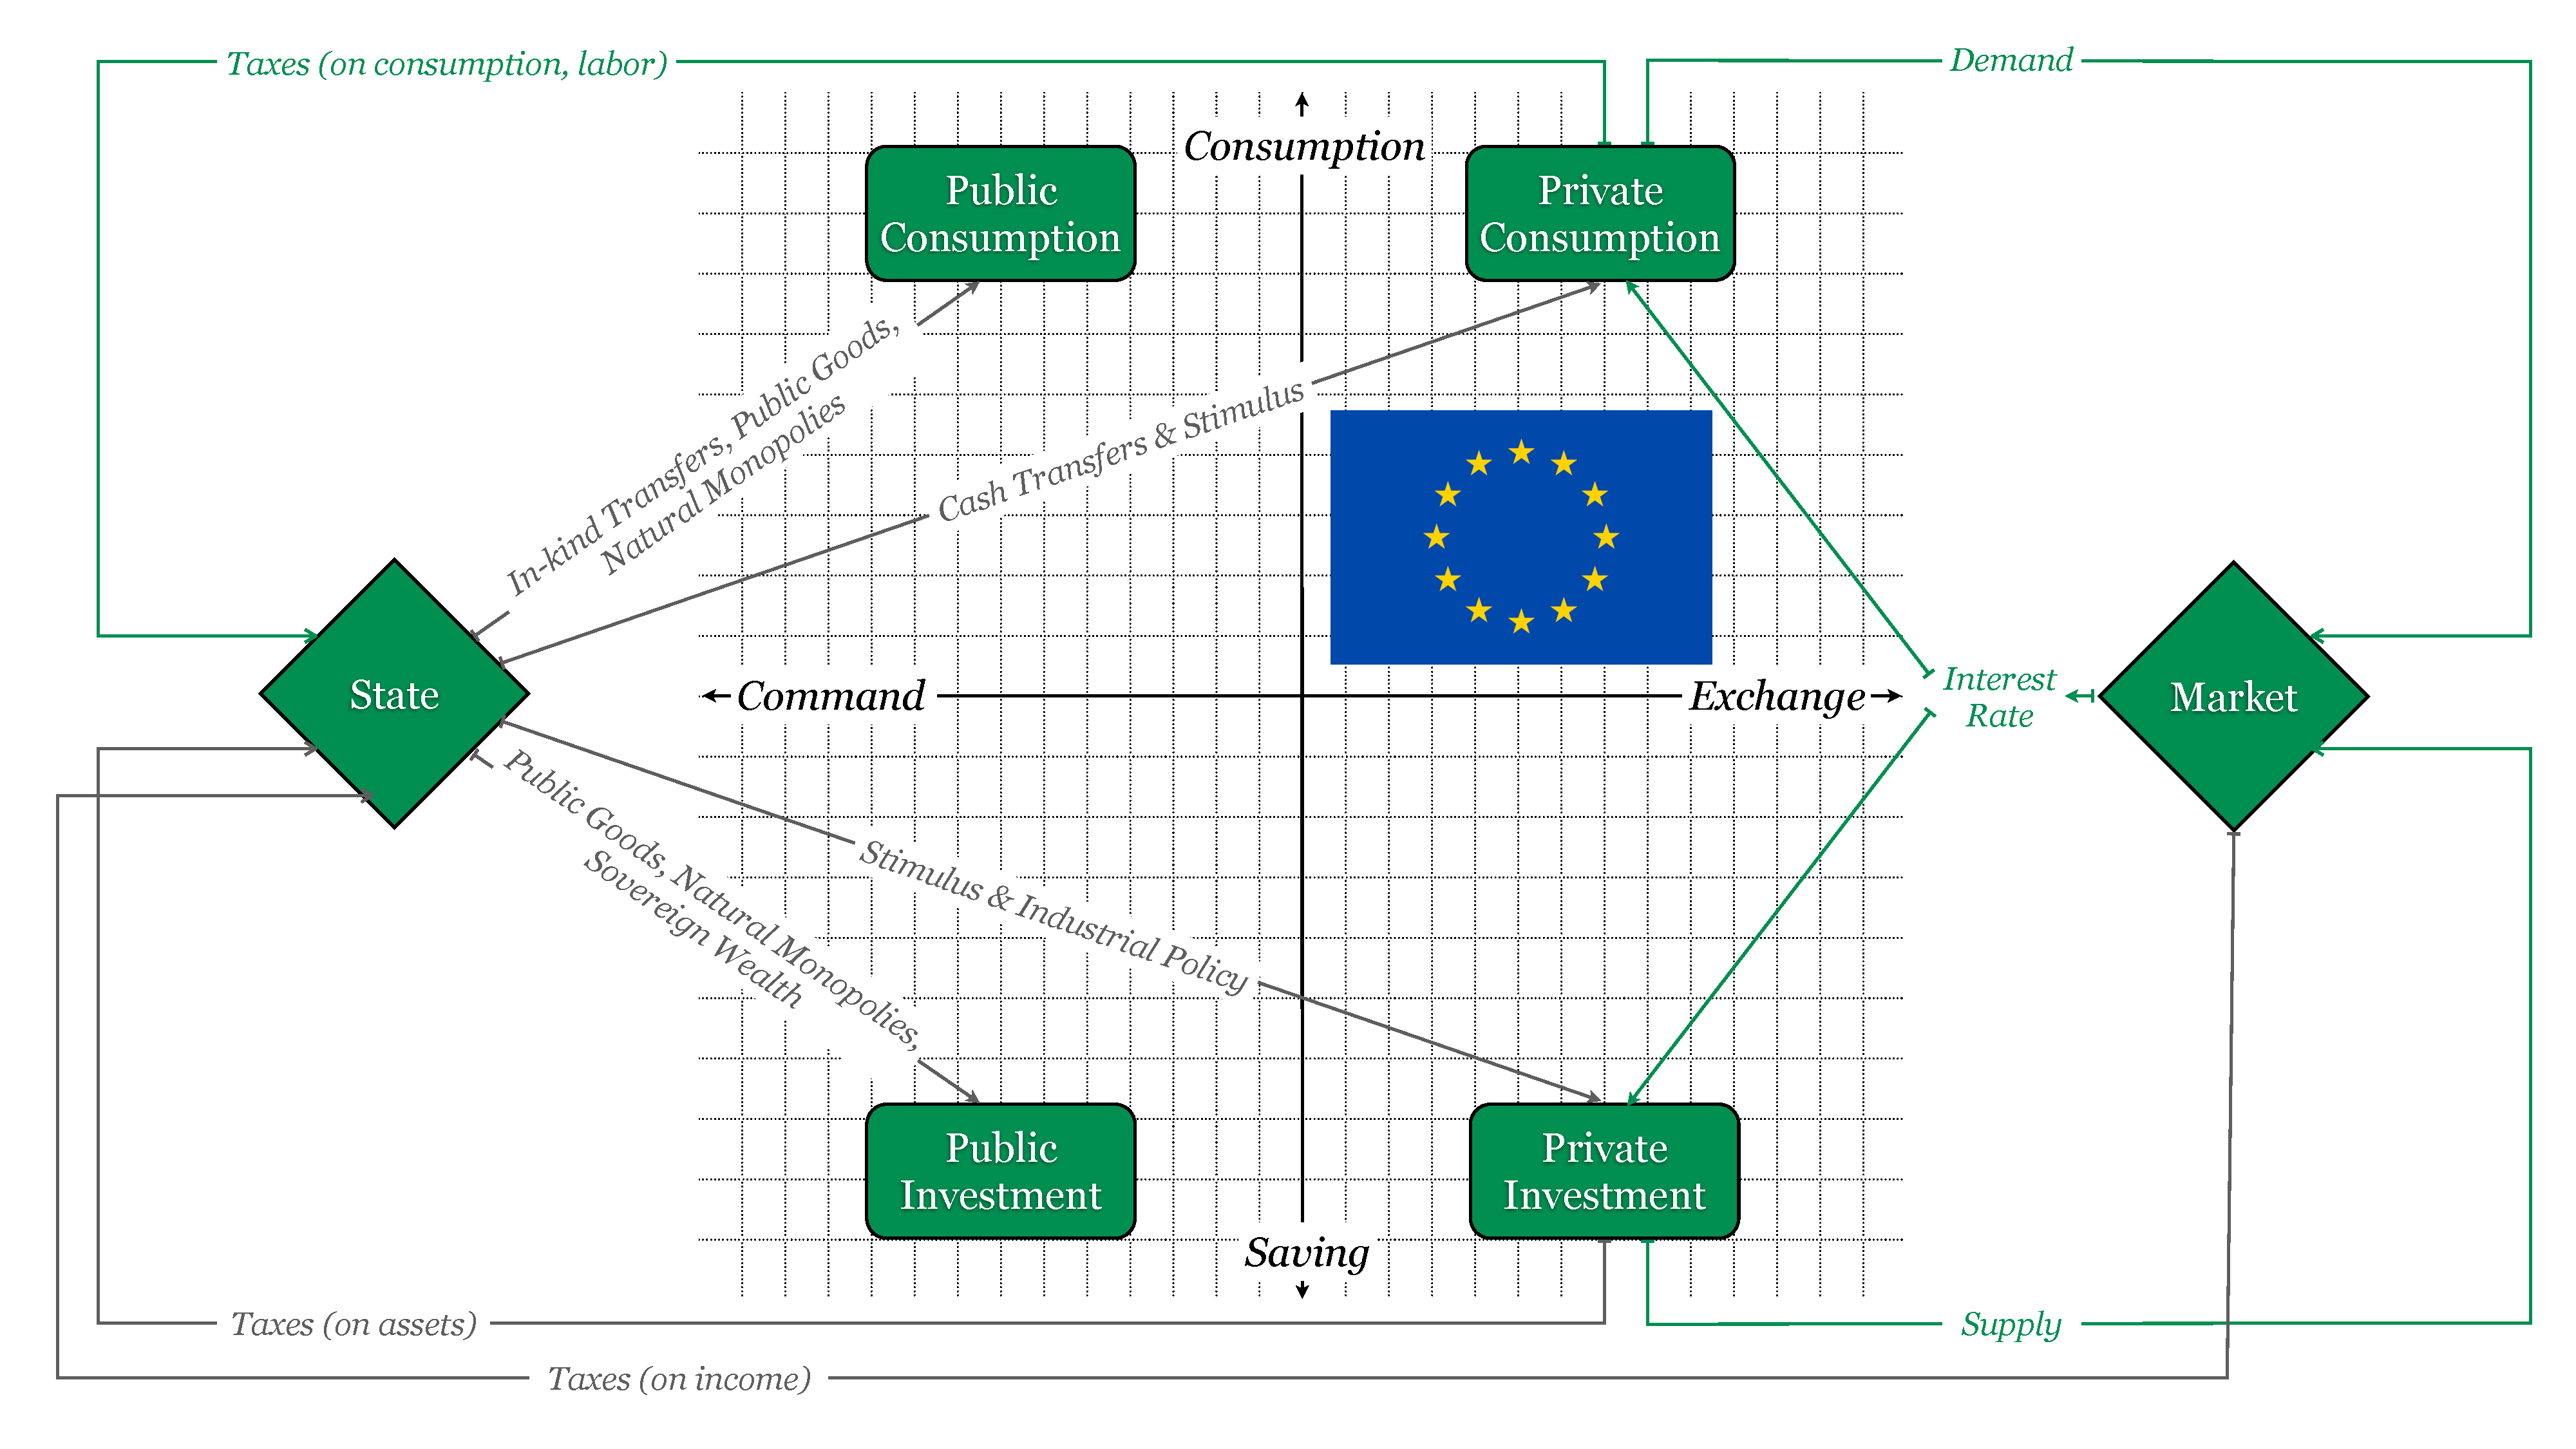
\includegraphics[width=1\textwidth]{coordinate-space-constrained}
	\caption{Constrained Coordinate Space of a Dysfunctional Mixed Economy}
	\label{fig:coordinate-space-constrained}
	\end{center}
\end{figure}

By its dysfunctional design, the european mixed economy yields ever more to markets while the other part of the mixed economy, the state, is on the retreat.
Bereft of their old, flexible and capable social contracts, the acquis will, nay, already \emph{has} --- however fortuitously --- remade european society in the neoliberal, consumerist image.
``Neoliberalism'' and ``consumerism'' are, in this case, not catch-all labels of disaffection, but I choose them with equal anger and care, and they apply precisely.
The aquis is:

\begin{description}
	\item[Neoliberal,]
	because, eviscerating the state, it morphs markets from one of several \emph{means}, to inescapable \emph{reality} or even ultimate \emph{end}, neither of which it is, nor should be.

	\item[Consumerist,]
	because, it cannot set a positive savings rate, and leaves austere members no choice but to loot real savings, and give into the temptations of bubbles.
	As a result, much of the resources of the communal household will be devoted to near-term consumption.
	\footnote{
		The \gls{eu} commission is quite explicit about this:

			\begin{quote}
				\emph{``The Single Market Review put \emph{(sic!)} citizens, consumers and \glspl{sme} at the centre of policy-making.''}
				\\*
				--- \citet[3]{Commission2008}
				%does this produce the correct citation?
			\end{quote}

		One wonders, at least, why, in addition to \emph{citizens}, consumers and \emph{some} (though not other) firms are also mentioned, when, in a functioning market, the latter two should be served only as proxies of the ultimate beneficiary, the citizen.
	}
\end{description}

Just how angelic the postwar mixed economy really was, I do not know.
\footnote{
	To mention just a few red flags, it is unclear what costs Postwar prosperity extracted from others (dependence or world systems theory), we do know whether or how Western affluence can be repeated without the same gigantuan carbon footprint and we worry whether broad-based growth in value-add is but a historical episode (cost disease).
}
Still, \emph{relative} to 19th century mass poverty \citep{MarxEngels-1848-aa}, 20th century ``mob politics'' \citep[158]{Crouch2004} and the spectre of 21st century neo-laissez-faire, the mixed economy, and the welfare state it has enabled, appears as singular achievements of the modern era.
The economic institutions of Postwar Western Europe have brought about unseen prosperity and equity, all in relative peace and freedom.

That is an old deal worth fighting for.

\subsection{Catch-Up}
\begin{quote}
	\emph{``Three tomatoes are walking down the street --- a poppa tomato, a momma tomato, and a little baby tomato.
	Baby tomato starts lagging behind.
	Poppa tomato gets angry, goes over to the baby tomato, squishes him, and says:
	catch up.''}
	\\*
	--- \href{http://www.youtube.com/watch?v=5D-QKY0-Bxk}{Mia Wallace in Pulp Fiction (1994)}
\end{quote}

Too easily, discontent with a retrenching Western European welfare state blames \gls{ceec} for ``social dumping'' %source
or otherwise slides into poorly disguised economic nationalism.
It must not:
whoever thinks that Western and Northern, otherwise intact mixed economies now whither away because of competition from the East and the South, misunderstands, or --- more likely --- misconstrues the issue.

Of course, the newly opened, low-productivity and low-capital markets in the poorer East and South have much lower, often proportional taxation, especially on capital incomes.
They \emph{cannot} afford high, or progressive taxes on capital, if they are to remain competitive, let alone converge.
\footnote{
	For example, L\'{a}szl\'{o} Kov\'{a}cs (2004), then Commissioner for Taxation and Customs asked that tax rates must be allowed to differ 6-8\% simply to make up for the remote location of some markets.
}
Had Romania the capital income taxation of pre-reform Sweden, the net returns on any investment would fall tremendously.
Given the low labor and total factor productivity in Romania, an investment might not be profitable at all, and capital might instead stay in high-tax, but also high-productivity Sweden.
Romania would not be able to attract much foreign capital, which it so direly needs to leapfrog into convergence.

By contrast, the high-productivity, high-capital markets in the West and North, \emph{could} afford higher, and more progressive taxes, if only they did not face tax competition from all other \gls{ms}.
Had Sweden the capital income taxation of post-accession Romania, or even the 0\% \gls{cit} of non-member Moldova \citep{Piatkowski2008}, it would have to abandon much of its mixed economy.
Forced to finance its large public sector only out of labor, or other immobile, proportional sources, the tax wedge on the lower and middle strata of society would become unbearable.
%add \href

At first sight, there appear to be only two policy responses to this conundrum:
\begin{enumerate}
	\item \emph{High European-Level Taxation.}
	\gls{ms} might agree to enforce union-wide, uniformly high and progressive taxes on mobile bases, that would save welfare in the rich \gls{ms}, but at the cost of laggard growth in the poor capital-deprived \gls{ms}.
	Such tax cooperation would save the welfare state, but sacrifice fast, or even any, convergence.

	\item \emph{Tax Competition.}
	\gls{ms} might continue with the status quo ante, set tax rates individually and let competition whither away levels and progressivity.
	Such tax competition would sacrifice the welfare state, but bring some convergence ``through the back door'' as rich \gls{ms} capital will to rush to poor \gls{ms}:
	poorer (and smaller) countries win under tax harmonization, as evidenced by their opposition to even nascent \gls{eu} tax cooperation \citep[138]{Kellermann2009}.
	\footnote{
		Capital inflows will be particularly effective in relatively poor economies.
		As these economies, supposedly, still lie far below the golden rule of saving \citep{Solow1956}, returns on capital will be much higher than in richer economies where further (near-Solowian) capital deepening faces diminishing returns (for example, \citealt{Barro1995} or \emph{ibid.} 1992 as cited in \cite[3]{Beckfield2009}.
	}
\end{enumerate}

Such are the alternatives that politicians might peddle, pitting poor members against rich, convergence between them against welfare within.
These are, as so often in defunct mixed economies, impossible choices to make, seemingly forcing European democracies to play a game of zero-sum.

Alas, regional economic integration, as all trade, is not zero-sum game:
there are gains to be had, if not accruing to everyone equally.
Sweden is better of for having a prospering, converging Romania as a trading partner, with different absolute or comparative advantage, capital endowments and areas of specialization.
Out of the proceeds of this positive-sum game, there is a third option:

\begin{enumerate}
	\setcounter{enumi}{2}
	\item \emph{High European-Level Taxation With Side Payments.}
	\gls{ms} agree to enforce union-wide, uniformly high and progressive taxes on mobile bases, but rich \gls{ms} recompense poor \gls{ms} for their ensuing competitive disadvantage.
	Absent different taxes rates on mobile factors, the union as a whole is able to choose freely amongst the trade-offs of a mixed economy, including a well-funded welfare state.
	Still facing low labor productivities, poor \gls{ms} receive fiscal transfers that they can use to build capital stock, educate their workforce, upgrade infrastructure, or even subsidize investment.
	For example, poor \gls{ms} might lower or even abandon taxation of some or all immobile factors, such as low-productivity labor.
	Facing a small or no tax wedge, maybe even receiving subsidized or free health care, or some other \gls{nit} of sorts, the low-productivity workers in poor \gls{ms} would be able to accept yet lower gross market wages, and become competitive again, even as investors have to pay high taxes.
	\footnote{
		To remind readers that this is not, in fact, what the acquis currently stipulates:
		The overall structural and cohesion funds for 2007--2013 amount to no more than \euro{} 347 billion, less than 3 times the budget of the city of Berlin (\euro{} 21 billion in 2009), or about 0.005 \% of the budget of Germany (\euro{} 1,164,000 billion in 2011).
		In addition, \gls{eu} budget negotiations are still marred by \emph{juste retoure} attitudes, with \gls{ms} wanting to get paid out what they have received --- the very opposite of a redistributive regime \cite[for example,][]{Begg2008a}.
	}

	Side payments need to be initially large enough but decrease over time, and they must be used wisely by poor \gls{ms}.
	As in any subsidy or  protection, it will be difficult to avoid long-term dependence and rent-seeking.

	If we get it right, though, high european-level taxation with side payments will save the mixed economy, enable a potent welfare state, clear factor markets, converge living standards in the union and keep us all on the long-term growth path.
\end{enumerate}

%add game theory here.
%Is there a game to be played?
%create a table about the options in the catch-up game.

We need not trade off openness and convergence \emph{between} \gls{ms} with efficiency and equity \emph{within} them.
In fact, they are the same issue:
behind the pressures on rich welfare states always lurks the question of convergence:
just how fast, and by which means, do we want the poor members to catch up?

If we opt for policy response
\begin{inparaenum}
	\item high european-level taxation, convergence will be minimal and through the market only.

	If
	\item we choose tax competition, convergence will be faster, and still only market-led.

	If we
	\item adopt high european-level taxation with side payments, convergence can progress at an arbitrary speed, with a substantial state component.
\end{inparaenum}

Deciding on the speed of the catching up may just be the deeper question of european integration that many politicians of all colors, but especially those tending to economic nationalism, may seek to avoid by misrepresenting european choice in dichotomous terms of more or less protection, more or less integration.
Convergence supported by side payments \emph{does}, of course, include a zero-sum component, as any redistribution by definition does.

But it is not, as it is easily made out to be, redistribution \emph{between} one economy and another, it is instead, redistribution \emph{within} one, European economy.
Whenever the markets expand beyond borders, so, too, the abstractions of the mixed economy rule at a higher level, and they apply not just to tax --- the clearest case that I have here illustrated --- but to all command interventions prone to arbitrage:
as the first good, service, or capital equipment crosses the border, the two trading partners have already adopted \emph{one} of the three regimes of economic integration, and, related, have made their however implicit choice of just how, and how fast, the poorer party gets to catch up.

The elephant in the room of european economic integration is this:
if we are to save the mixed economy, we have to explicitly decide, not just agree by default, how fast we want to converge.
\footnote{
	It too, is neither new nor revolutionary:
	internally heterogenous mixed economies have always, with varying results, dealt with this question.
	In the US, much of the controversy about the role of the federal government boils down to the question of how much rich Texans should dole out to poor Louisianans.
	In Italy, the rift is between North and South \citep[for example,][]{PutnamLeonardi-1993-aa}) and in Germany, initially between industrial and rural states, since 1990 between old and new \emph{Laender}.
}
%On the old deal:
%the imbalances and dysfunctions of the potent mixed economy provide fuel for the cyclical, and now fairly grave fin market crises.
%Without this fuel, these crises would not build.
%But, they are not the only problem, nor are they the only thing we should fixate on in avoiding crises.
%We also need macro prudential oversight and regulatory intervention to fight the market failures that lie at the heart of financial crises.

%\section{So, you Want a Revolution?\ldots} \label{sec:Revolution}

%\begin{quote}
%	\emph{So, you want a revolution?\\*
%	Well, you know:
%	We all want to change the world.}\\*\\*
%	The Beatles (1980)
%\end{quote}

%Yes, the PCT would be a revolutionary overhaul of tax, redistribution and economic production.
%But no, this is not socialism, or anything of the kind.
%Even if I have my way, there will still be \hyperref[des:Entrepreneurship]{private ownership of the means of the production}.
%And there should be, as per desideratum \ref{des:Entrepreneurship}.

%But still, this is a normative project as much as it is an analytical project.
%It is as much policy as it is social science.
%I do not want to apologize for that.

%After two years of studying at the \hyperref[http://www.hertie-school.org]{Hertie School of Governance}, \hyperref[http://maxheld.de/2009/10/13/setting-goalposts/]{``disinterested'' just does not cut it anymore}.
%If social science and policy analysis does not want to end up being latently affirmative, it should start asking the status quo a little harder, and a little more creative questions.

%Here is one.

%\subsection{The Fierce Urgency of Taxation} Tax is not boring, and tax is not inconsequential.
%In fact, ``tax represents the last battle line for any meaningful redistribution of material resources from the better able to the least well off'' (\citealt{McCaffery2005}:
%936).

%We should be grateful that this last battle line lies in the abstractions of tax, and is no longer violently fought in revolutionary strife.

%But this last battle line must not be abandoned, nor retrenched.
%Much is at stake.
%With a defunct fiscal configuration, our polity is paralyzed.
%For, as the conservative Edmund \citeauthor{Burke1790} remarked, ``[t]he revenue of the state \emph{is} the state'' (\citeyear{Burke1790}:
%111, emphasis added.).

%The PCT was first suggested in the 1940s, to curb inflationary tendencies in a time when government expenditure \emph{could} not be reduced (\citealt{Cheng1953}:
%333).
%The United States were at war, everywhere against the axis powers, later, in Korea, then in a Cold War of hemispheric scale.
%The American polity needed greater saving, and more public goods (defense, after all, is the quintessential public good).

%My point is this:
%we are \emph{there} again.
%With no war, at least on our continent, but with widespread unemployment, lagging growth, rampant social problems, an education with too little, too unequal opportunity for many, and a planetary system thoroughly out of balance --- we are \emph{there} again.

%The Progressive Consumption Tax returns to the polity, what is hers:
%the ability to democratically decide how much we want to save for our children, how large the sticks and carrots should be today, how we want the economic pie to be sliced, and what we want it to be used for.
%Let us reclaim that enlightened emancipation:
%that really, how we live together \emph{is} of our own, collective choosing.
%\emph{That} is the project of the \hyperref[http://www.policy-net.org/blogs/thepotentpolity]{potent polity}, to which I here wish to contribute.

%These are no abstract considerations.
%Right beneath the surface of tax lie the life chances of people.
%The immigrant schoolgirl in Berlin-Kreuzberg, who needs her public school to be a palace of learning and self-fulfillment.
%The management consultant who did not make the promotion, and cannot afford the luxurious trip to the Seychelles with his girlfriend.
%The cancer patient who needs her disease to be better understood, and cured.
%Our polity's ability to tax, to finance and to redistribute makes all these lucks, and all our luck, too.

%To live up to the potential of our progress, and to honor the promise of our democracy we must reunite what \emph{is not} antithetical:
%rigorous competition, high productivity, a well-equipped polity and robust redistribution.

%If we get tax right, we can have it all:
%``to prosperity and opportunity'', indeed.

\section{Why Tax Matters to Democracy}

\begin{quote}
	\emph{``But who can say how much is endurable, or in what direction men will seek at last to escape from their misfortunes.''}
	\\*
	--- John Maynard \citet{Keynes1936}
\end{quote}

\begin{quote}
	\emph{``
	%``I'm still trying to climb out from under the avalanche of horror, nightmare and disgust that all of this [the 2011 US debt ceiling crisis] dumped on me, along with, I suppose 300 million other Americans and it's a little hard to sort out your thoughts after this much awfulness comes along.
	%[\ldots]
	%Sorry but I actually do think that this [the 2011 US debt ceiling crisis] is one more symptom of a long, slow constitutional crisis, it goes back further than the 2000 election.
	%This kind of thing keeps happening again and again, it's as if our system is getting hardening of the arteries, we get a stint once in a while [\ldots] but to me it's getting scarier and scarier over the long haul.
	%[\ldots]
	There are a lot of rational (tax) ideas out there, there are a lot of ways you could build something from scratch that would look roughly like the society we have now, but would work better, would be smoother and fairer and all that.
	And of course, these things are proposed in politics [\ldots] and then they cannot be done.
	Then our system prevents them from happening or garbels them in such a way that they look supremely ugly, once they are created [\ldots].
	This is a machine for creating disillusionment with government, cynicism, Tea-Partyism, and over time, this is our county, our democracy eating itself alive.
	[\ldots]
	And that's why I get a little discouraged sometimes.''}
	\\*
	--- Hendrik Hertzberg (2011) on The New Yorker podcast \emph{The Political Scene}
\end{quote}

%(Both of this is Foreword ix, in Esping-Andersen 2002)
	%“The irony (of structural transformation and existing welfare programmes) is that class may be less visible, but its importance is arguably far more decisive.
%(…) The post-war welfare state no doubt succeeded in equalizing living conditions, but it failed to deliver on its promise of disconnecting opportunities from social origins and inherited handicaps.” (ibid:
%3)
	% This I like, a lot:
%“(…) there is a very good argument that equality of opportunities and life chances is becoming sine qua non for efficiency as well.”
	%	-         “de-familialization” is an ugly word, but necessary nonetheless.

%Not sure I agree with crouch that we want back the class in itself working class, that may be misconstruing the past and we don't really want that today.
%Think about that.
%Also note that even crouch misunderstands the taxation of firms.

%Cite Eliasoph on why we need a big ass issue;
%not a small scale issue.
%You're leading to despondence.
%Quote early passages of Eliasoph.
%Also argue with Eliasoph "Charles said …" that by all means trying to CHANGE things, and only discuss things you can change, has drawbacks.

%[ ]  also:
%markets are an incentive-driven form to organize activity.
%This is all good and well, but an incomplete view of the ability of humans to produce.
%The deliberative model is another way to do this.
%It's kind of the synthesis:
%it abandons rational motivation, but it still features the abstractions that govern complex, rich socieities.

%from europe piece

%Cite Young's critique of deliberation as support for "hypothetical".

\section{The Social Contract}
%---
%Martin, I.
%W., Mehrotra, A.
%K., & Prasad, M.
%(2009).
%The Thunder of History - The Origins and Development of the New Fiscal Sociology.
%In I.
%W.
%Martin, A.
%K.
%Mehrotra, & M.
%Prasad (Eds.), The New Fiscal Sociology - Taxation in Comparative and Historical Perspective.
%Cambridge, UK:
%Cambridge University Press.
	%1:
%"In the modern world, taxation is the social contract."

%here comes another copy/paste from the europe piece

Crucially, we must, again, understand that economic integration must always beget more economic and political integration, that, production at great economic scale implies solidarity at the same scale.

\emph{That} is the story of economic integration and material progress.
Living on a scarce and harsh planet, for which, alone, we are ill-equipped, we escaped the \citeauthor{Malthus1798}ian curse of overpopulation and starvation by scaling up our production.
That is, to this day, how we remake an arithmetically growing material world, to feed our geometrically growing hunger:
we join forces to bend upward the production curve, and wrest from it above-linear returns.
To reap such economies of scale, in agriculture \citep{Diamond1997}, in the production of violence \citep{Tilly-1985-aa}, or in europe-wide automotive engineering \citep{Krugman-1980-aa}, we have to master the feat of cooperation in the face of atomistic incentives.
Akin to ever-increasing entropy, the arrow of pre-historic organic life, and history of human life on earth progresses by increasing complexity, specialization, but also, always, mutual dependence.
\citeauthor{Wright1994} thus describes the transformation of individual cells into higher organisms:
they become richer, more resilient, but they must also sacrifice, and will do so only to the extent that they have successfully merged their genetic instructions \citeyearpar[Chapters 7, 8]{Wright1994}.
%better double-check this stuff.
%This isn't quite right yet.

And so it is with european, or other regional economic integration:
opening up commerce to one common market makes everyone richer by the magic of comparative advantage --- if not necessarily by the same amount.
But, if this association is to remain stable, some other elements of human organization have to follow to that higher level, if they are not to perish and destabilize.
In the \gls{eu}, continent-wide commerce also requires continent-wide taxation, regulation and monetary policy, if the formerly stable and re-productive system of a mixed economy is to remain operative.

The genius of the otherwise hyper-federal, and hyper-liberal US Constitution is that it foresees this functional necessity in its commerce clause.
\footnote{
	\ldots the reach of which was only recently discussed in the 2012 US Supreme Court ruling on the Affordable Care Act.
}
It stipulates that, precisely as commerce traverses the otherwise autonomous states, the federal polity asserts itself.
The German constitution knows a similar norm:

\begin{quote}
	\emph{``The Federation shall have the right to legislate on matters [\ldots] if and to the extent that the establishment of equivalent living conditions throughout the federal territory or the maintenance of legal or economic unity renders federal regulation necessary in the national interest.''}
	\\*
	--- Basic Law for the Federal Republic of Germany:\ Article 72, Paragraph 2 (Bonn, 1949)
	\footnote{
		In the German original:
		\begin{quote}
			\emph{``Auf den Gebieten [\ldots] hat der Bund das Gesetzgebungsrecht, wenn und soweit die Herstellung gleichwertiger Lebensverhältnisse im Bundesgebiet oder die Wahrung der Rechts- oder Wirtschaftseinheit im gesamtstaatlichen Interesse eine bundesgesetzliche Regelung erforderlich macht.''}
			\\*
			--- Grundgesetz der Bundesrepublik Deutschland:\ Artikel 72, Absatz 2 (Bonn, 1949)
		\end{quote}
	}
\end{quote}

It too, displays the same genial insight into the relationship between economic and political integration:
as the commerce clause, it does not compel any particular social or other policy, but, if economic integration has occurred, endows the democratic sovereign to rule at the newly emerged, higher level of societal organization.

%some of the following will have to go
\section{Growth and Solidarity} \label{sec:growth-solidarity}

\begin{quote}
	\emph{``The Congress shall have Power [\ldots] To regulate Commerce with foreign Nations, and among the several States, and with the Indian tribes''}
	\\*
	--- Constitution of the United States:\ Article I, Section 8, Clause 3 (known as the Commerce Clause) (Philadelphia, 1787)
\end{quote}

Let me now return to the first order perspective:
what, from here, is to be done about european integration and its failing welfare states?

Crucially, we must, again, understand that economic integration must always beget more economic and political integration, that, production at great economic scale implies solidarity at the same scale.

\emph{That} is the story of economic integration and material progress.
Living on a scarce and harsh planet, for which, alone, we are ill-equipped, we escaped the \citeauthor{Malthus1798}ian curse of overpopulation and starvation by scaling up our production.
That is, to this day, how we remake an arithmetically growing material world, to feed our geometrically growing hunger:
we join forces to bend upward the production curve, and wrest from it above-linear returns.
To reap such economies of scale, in agriculture \citep{Diamond1997}, in the production of violence \citep{Tilly-1985-aa}, or in europe-wide automotive engineering \citep{Krugman-1980-aa}, we have to master the feat of cooperation in the face of atomistic incentives.
Akin to ever-increasing entropy, the arrow of pre-historic organic life, and history of human life on earth progresses by increasing complexity, specialization, but also, always, mutual dependence.
\citeauthor{Wright1994} thus describes the transformation of individual cells into higher organisms:
they become richer, more resilient, but they must also sacrifice, and will do so only to the extent that they have successfully merged their genetic instructions \citeyearpar[Chapters 7, 8]{Wright1994}.
%better double-check this stuff.
%This isn't quite right yet.

And so it is with european, or other regional economic integration:
opening up commerce to one common market makes everyone richer by the magic of comparative advantage --- if not necessarily by the same amount.
But, if this association is to remain stable, some other elements of human organization have to follow to that higher level, if they are not to perish and destabilize.
In the \gls{eu}, continent-wide commerce also requires continent-wide taxation, regulation and monetary policy, if the formerly stable and re-productive system of a mixed economy is to remain operative.

The genius of the otherwise hyper-federal, and hyper-liberal US Constitution is that it foresees this functional necessity in its commerce clause.
\footnote{
	\ldots the reach of which was only recently discussed in the 2012 US Supreme Court ruling on the Affordable Care Act.
}
It stipulates that, precisely as commerce traverses the otherwise autonomous states, the federal polity asserts itself.
The German constitution knows a similar norm:

\begin{quote}
	\emph{``The Federation shall have the right to legislate on matters [\ldots] if and to the extent that the establishment of equivalent living conditions throughout the federal territory or the maintenance of legal or economic unity renders federal regulation necessary in the national interest.''}\\*
	--- Grundgesetz der Bundesrepublik Deutschland:\ Artikel 72, Absatz 2 (Bonn, 1949)
	\footnote{
		In the German original:
		\begin{quote}
			\emph{``Auf den Gebieten [\ldots] hat der Bund das Gesetzgebungsrecht, wenn und soweit die Herstellung gleichwertiger Lebensverhältnisse im Bundesgebiet oder die Wahrung der Rechts- oder Wirtschaftseinheit im gesamtstaatlichen Interesse eine bundesgesetzliche Regelung erforderlich macht.''}\\*
			--- Basic Law for the Federal Republic of Germany:\ Article 72, Paragraph 2 (Bonn, 1949)
		\end{quote}
	}
\end{quote}

It too, displays the same genial insight into the relationship between economic and political integration:
as the commerce clause, it does not compel any particular social or other policy, but, if economic integration has occurred, endows the democratic sovereign to rule at the newly emerged, higher level of societal organization.

%add more from the Papier debate here?

What the \gls{eu} needs, is not more stringent subsidiarity, but it's inverse:
a commerce clause.

%here used to be \ref{sec:LD-Difference} part, now only in better democracy

%\subsection{Postwar}

%\begin{quote}
%	\emph{``Meanwhile [in 1989], across the Leitha and Danube rivers just a few kilometres to the east, there lay the ‘other' Europe of bleak poverty and secret policemen.
%The distance separating the two was nicely encapsulated in the contrast between Vienna's thrusting, energetic Westbahnhof, whence businessmen and vacationers boarded sleek modern expresses for Munich or Zurich or Paris;
%and the city's grim, uninviting S\"{u}dbahnhof:
%a shabby, dingy, faintly menacing hangout of penurious foreigners descending filthy old trains from Budapest or Belgrade.''}\\
%	--- Tony \citeauthor{Judt2006} (\citeyear{Judt2006}:
%5)
%\end{quote}

%!marginpar
%\marginpar{Because this section is so small and I have so little to say on it, it might better go.
%I just love the Judt quote.}

%In his epic Postwar tome, \citeauthor{Judt2006} chronicles the divergent paths that drove apart eastern and western Europe, as the post-war settlement inflicted on them the historical accident of Cold War division.
%The wounds of this continental tear have not healed, in fact, until and unless we install democratically governed, intact mixed economy on the continent, it will continue to pain and undermine the union, only superficiously covered by the paltry Band-Aid of the common market.

%If there is a Postwar history to building welfare states in \gls{ceec} is that so far, they will only succeed if we finally close the tear of 40 years of state socialism, and agree on how fast to have the East catch up, and how to make it happen.

\subsection[Weimar]{Weimar}

%via MPP on inefficient inequality
	%\paragraph{Extreme Inequality May Lead to Instability, Threaten Democracy}
	%this might have to go somewhere else.
%This is in the wrong place.
	%Democracy and peaceful resolution of societal contradictions have emerged in tandem with economic growth \emph{and} redistribution \citep{Marshall-1950-aa}.
%There are empirical findings that suggest that this link may still operate today.
%The political sociology of modernization theory suggests that economies, political institutions and mass values evolve \emph{together}, in a project of ever increasing human emancipation \citep{InglehartWelzel-2005-aa}.
%These links hold both at the societal and at the individual level:
%more materially affluent people are more likely to hold pro-democratic mass beliefs, including generalized trust \citep{KnackKeefer-1997-aa}, tolerance, and self-actualization \citep{InglehartWelzel-2005-aa}.
%Other, structural(ist) formulations of this link stress the importance of \emph{cross-cutting cleavages} for functioning democracy \citep{LipsetRokkan-1967-aa}.

%\begin{quote}
%	\emph{``There’s a storm coming, Mr.~Wayne.
%You and your friends better batten down the hatches.
%Because when it hits you’re all going to wonder how you ever thought you could live so large and leave so little for the rest of us.''}\\
%	--- Selina Kyle (``Catwoman''), Dark Knight Rises (2012)
%\end{quote}

\begin{quote}
	\emph{``But who can say how much is endurable, or in what direction men will seek at last to escape from their misfortunes''}
	\\*
	--- John Maynard \citet{Keynes1936}
	%duplicate
\end{quote}

Optimists, not just of the Panglossian kind, are always inclined to see glasses half-full, and so many argue that any, even imperfect or negative European integration is better than none.
 That is not so much optimistic, as it is hopelessly naive.
The metaphor is flawed.
Societies are not just glasses half-full or half-empty, they are dynamic systems, residing within, and reproducing the walls of this glass:
half-\emph{built} glasses, as the \gls{eu} defunct mixed economies, are not merely waiting to be filled, they can also drain of all remaining water, or topple and fall over.

The democratically governed mixed economy is \emph{the} institutional achievement of the century, and as a social compact, it is fragile.
As \citeauthor{Offe2003} points out, ``it is much more likely that a European-styled [mixed economy] capitalism transformed itself into a liberal model'' than the other way around, or, appropriating Lech Walesa, ``it is easier to make fish soup out of an aquarium than the other way around'', because it --- like the mixed economy --- depends upon ``supportive dispositions of a cognitive as well as moral kind'' \citeyearpar[446]{Offe2003}.
A mixed economy, as the democracy that governs it, is ``easily lost, but never finally won'', as the first African-American federal judge William H.~Hastie ominously warned.

We have already lost much of the mixed economy, and we are now risking to harm or loose democracy, too:
not just democratic rule \emph{of} the \gls{eu}, but democracy \emph{in} Europe, too \citep[19]{Scharpf1997}.

Democracy needs not just a legitimacy of inputs, but also of outputs (on Europe see \citealt{SchaGove1999}).
In \citeauthor{Dahl-1994-ab}'s (\citeyear{Dahl-1994-ab}) terms, democracies need to be ``system effective'', in \citeauthor{Zurn-2000-aa}'s \citeyearpar{Zurn-2000-aa} apt words, democracies need to be ``output congruent'':
people must be able to choose any (liberal) policy they want to govern a given polity.
The \gls{eu}, currently violates output congruency:
with an impotent, largely defunct mixed economy, the people of Europe cannot have all materially possible policies to improve their currently grim life chances, including crushing trade imbalances, demoralizing structural unemployment, wild economic cycles, public squalor and rampant inequality.
In the half-built, supposedly \emph{sui generis} glass of Europe, there is a wide mismatch between the two walls:
the exchange components of the mixed economy roam the continent, while most of the command components are confined to the constrained nation state.
As a result, the glass is heavily leaking water, both in efficiency and equity.

Over time, the hardship that this arrangement inflicts on people, especially in the poorer, more austere \gls{ms} (Greece), and when the imbalances and crises unload (Spain, Ireland), will corrode the inputs of popular rule, too, and fray the social contract.
\citeauthor{Offe2003} has already seen the grave-diggers of liberal democracy, capitalizing on the resulting popular discontent of such ``permanent austerity'' \citep{Streeck2010c}:
\begin{quotation}
	\emph{``Also, a third voice, luckily with much less resonance, is making itself increasingly heard in European politics, a voice which claims that the social security of workers (as well as the protection of citizens from violent crime), on the one hand, and efficiency of production and competitiveness, on the other, can only be reconciled if national borders are sealed to the influx of foreign people, foreign workers, foreign goods, and those praying to `foreign' gods.
	Since the mid-1990s, integrating Europe has seen the sometimes sudden and spectacular rise to electoral success of figures such as Pia Kjaersgaard (Denmark), Umberto Bossi and Gianfranco Fini (Italy), Pim Fortuyn (Netherlands), with Jean Marie Le Pen (France), Jörg Haider (Austria) and Carl Hagen (Norway) being among the pioneers of this new field of populist political entrepreneurship.
	Le Pen has described himself in the 2002 French electoral campaign as being a leftist in social affairs, a rightist in economic affairs, and a nationalist for everything else.
	\\
	This formula, which is designed to resolve the tension between liberal market freedom and welfare state status rights by ethno-nationalist, xenophobic, and anti-European appeals, is applied by his rightist populist colleagues as well."}
	\\*
	--- Claus \citet[454]{Offe2003}
\end{quotation}

The ground of popular resentment will only grow more fertile as the Euro crises goes on.
The crippling economic depressions of the south, and the ever-insufficient, multi-billion bail-outs from the north are political dynamite, waiting to be ignited by fringe populists.

If the extreme right, or extreme left, and/or nationalists start playing with this fire, the moderate voices of social democracy, liberalism and conservativism will have little to douse the flames, because in fact, both the polities in the north and south \emph{are} faced with thoroughly unattractive alternatives.

In the now often wretched south, policy makers must either accept the conditional straightjacket imposed by the \gls{eu} and its rich sponsors, or jump the cliff of secession and sovereign default, all but ensuring all-out economic collapse under autarky.
In the still largely isolated north, policy makers must either continue to periodically support often (but not always) failing governments in the south to alleviate the gravest imbalances, or splinter the union and forego the years, maybe decades of economic growth that wide integration brought.

European democracies thus are also no longer \emph{input congruent} \citep{Zurn-2000-aa}, in addition to the already grave, but homemade democratic deficit of a heavily intergovernmentally-biased institutional setup.
Faced with such non-alternatives, the people of Europe are no longer subjected only to decisions in the making of which they had a say.
For the past two years, every couple of months, German or Greece executives, legislators and voters are asked to choose between bail-out or break-up, austerity or abyss, always at gunpoint, with the entire european project held hostage (for example, \emph{Grexit}, followed by Portugal, Spain, Italy, followed by doomsday).
If the people of Europe merely get to choose between a rock and a hard place, popular sovereignty becomes a farce.

\citeauthor{Offe1998}'s \citeyearpar{Offe1998} intuition is, tragically, fully borne out:
\begin{quote}
	\emph{``[\ldots] that every interim solutions between the extremes of intact national sovereignty on the hand, and complete european supranationalty of a European Federation will, inevitably, violate both the reference point of welfare state protection and that of democratic legitimacy.''}
	\\*
	--- Claus \citet[41]{Offe1998}
	\footnote{\label{fn:Offe-regress}
		In the German original:
		\begin{quote}
			\emph{``Meine These ist, dass jede Zwischenlösung, die zwischen diesen beiden Extrempolen intakter nationalstaatlicher Souveränität einerseits, einer kom-plettierten europäischen Supranationalität in der Gestalt eines föderalen eu-ropäischen Staates andererseits gefunden wird, zwangsläufig beide Be-zugswerte verletzt, den des wohlfahrtsstaatlichen Schutzes ebenso wie den der demokratischen Legitimation.
			Demnach könnte man im Blick auf die europäische Integration einen Abstieg auf jener Leiter vermuten, die T.~H.~\cite{Marshall-1950-aa} sich als Modell für den Prozess der europäischen politischen Modernisierung vorgestellt hat.
			Die drei Stufen dieser Leiter sind bekanntlich die kumulative Durchsetzung liberaler, demokratischer und sozialstaatlicher Rechte.
			Die Frage ist, ob im Prozess der europäischen Integration die demokratische und die sozialstaatliche Stufe in rückwärtiger Richtung passiert werden und im Ergebnis der Euro-Bürger allein mit der Rechtsausstattung eines (neo-)liberalen Marktteilnehmers dastehen wird.''}
			\\*
			--- Claus \citet[41]{Offe1998}
		\end{quote}
	}
\end{quote}

The political fringes will prosper, as they exploit these violations, both from the extreme left and the extreme right.
The extreme left will fan the flames of societal disintegration by pitting liberal freedoms --- especially those of property and contract! --- against welfare protection and democratic sovereignty.
Merely a change in tone, the extreme right will push societal regress by pitting all cosmopolitan integration and solidarity against always national welfare and sovereign rule.
This new game is rigged against liberal democracy and the moderate voices (or cross-cutting cleavages, \citealt{LipsetRokkan-1967-aa}) on which it so thoroughly depends.

What the glass-half-full-optimists forget is that societal, political and economic integration can reverse course, too.
The self-reinforcing dynamics of integration operate in \emph{both} directions:
more integration begets more integration (as Monnet had hoped, according to \cite[948]{Schmitter1999}, but regress also begets more regress.
As a matter of fact, the neo-functionalists are right, if one-sided (Tranholm-Mikkelsen 1991 as cited in \citealt[1]{Bieler2003})

The course of economic disintegration is quite clear:
literally the milli-second that an over-indebted \gls{ms} is thought to leave the \gls{emu}, anticipating massive devaluation, all holders of cash in, say, Greek institutions, will take their money out.
\footnote{
	In fact, the run on Greece is already underway, with the country having lost almost a third of its domestic bank deposits by May 2012, according to \cite{TheEconomist2012}.
}
Faced with such an economy-wide bank run, the Greek government will be forced to install capital controls, effectively leaving the common market.
Without international finance, the remaining trade, too, will be greatly constrained.
Just the credible rumor of \emph{Grexit} could, thereby, almost in an instant, unravel 21 years of integration since the country joined in 1981.

We tread the course of political disintegration if --- outflanked by populists --- our \gls{ms} democracies increasingly re-embrace the supposed trade-off between national interest and political unification, and again entertain the nationalist politics that the union was built to overcome, in a scenario of decay similar to that painted by \cite[339ff]{BeckGrande-2007-aa}, or \cite[947]{Schmitter1999}.

Writ large on society, this is the disintegration that \citeauthor{Offe1998} presciently feared in \citeyear{Offe1998}:
\begin{quote}
	\emph{``[\ldots] one could suspect a downward descent on the ladder that T.~H.~\cite{Marshall-1950-aa} suggested as a model for european political modernization.
	The three rungs on this latter are the cumulative expansion of liberal, democratic and social rights.
	The question is, whether during the course of european integration, we will pass the democratic and welfare state stages on our way down, and, as a result, european citizens will be equipped merely with the rights of a (neo-)liberal market participant.''}
	\\*
	--- Claus \citet[41]{Offe1998}
	\footnote{
		For the german original, see footnote \ref{fn:Offe-regress}.
	}
\end{quote}

We have been here before:
1918.
Torn apart by nationalist antagonisms and frayed by beggar-thy-neighbor responses to depression, economies \emph{can} disintegrate, as the havoc-wreaking de-globalization of the interwar years showed.
Strangled by economic depression, convulsed by trade and monetary imbalance, enslaved by material hardship and disheartened by a political system that would not and could not offer remedy, liberal democracies \emph{can} crumble into such mob rules as fascism or stalinism, as people, in their despair, turn to the easiest answers.

It does not take another genius to, as \cite{Keynes1936} did in 1918, anticipate the economic consequences of this particular peace, and to recognize how fragile this mode of one-sided, one-legged, market-only European integration is.
It is both the greatest strength and greatest weakness that democracy, to thrive and to persist, must be able to complement market production and distribution with a plan.
Whether in the German Empire, New Deal America or  Postwar West Germany, when under --- or just forestalling --- popular rule, the societies of Bismarck, FDR/LBJ and Adenauer/Erhard always matched competitive markets with strong states, each for their own reasons:
to ward off democracy \citep{Leibfried}, to protect it from the robber barons \citep{Wapshott2011}, or to compete with a socialist neighbor \citep{Judt2006}.

To this day, not a single developed, liberal democracy has withstood the test of time, that did not stand firmly on \emph{two} legs, one of market exchange, and one of state command.
Those who relied merely on command disgraced themselves in corruption, waste and totalitarianism.
Those who relied merely on exchange crumbled under the assault of extremists, and inequality.

Compared with even the most market-liberal (merely electoral) democracy, the United States, the European Union is a one-legged cripple of a mixed economy (for example, \citealt{Bordo2011}).
It does not even have a commerce clause, or union-wide bonds.

We have seen before, where one-legged polities can stumble:
in the two-fold 31-year war that ravaged the world after 1914 and the singular catastrophe of Hitler Germany.

This is not alarmism, this what the precautionary principle demands of us.
If everything is at stake, you do not run the risk of even half-full, half-built glasses.

That, especially, is the burden borne by Germans of every generation after 1945, who,
\begin{quote}
	\emph{``Conscious of their responsibility before god and men, inspired by the determination to promote world peace as an equal partner in a united Europe [\ldots]''}
	\\*
	--- Preamble of the Basic Law for the Federal Republic of Germany (Bonn, 1949)
\end{quote}
must never again leave an impaired polity to be preyed on by the vultures of liberal democracy, always lurking at the fringes.
Germans, above all, should cherish the mixed economy, insist that european integration be thus righted and show the solidarity with other \gls{ms} on which their post-1945 economic and democratic miracle thrived and, to this day, utterly depends.

That, too, is the spirit to which all peace loving nations have subscribed,
\begin{quote}
	\emph{``[\ldots] to save succeeding generations from the scourge of war, which twice in our lifetimes has brought untold sorrow to mankind [\ldots]''}
	\\*
	--- Preamble of the Charter of the United Nations (San Francisco, 1945)
\end{quote}
and that now, must be re-kindled:
that everywhere and always, a social contract to preserve peace, liberty and prosperity, is a fragile achievement, that must not be thoughtlessly abandoned.

Negative regional integration always puts in peril that social contract.
If a united Europe is to be the exception to its own history of war and terror, it must not stop at the half-way point.
If it is to stay, it must complete full, positive integration, re-grow the limbs of an effective mixed economy and take to heart the lessons of Weimar:
never again must we stay stranded on one leg, half of the way, for we may fall back and loose it all.

%[ ] Peter Hall says right wing parties exploit people's diffuse discontent with their living confidence

	%These internal challenges, however, do not call into question the principal ability of the state to organize welfare, they keep congruent input and output of the decision-making process and the affected citizens in the field of welfare (Zürn 2000).

	%At the very heart of the external challenges to welfare states lies the violation of congruency between political process and affected constituency.
%Critics of globalization argue that the liberalization of trade in goods and services and increasing factor mobility (capital, technology, to a lesser extent labor) restrict the ability of states to organize redistribution and risk pooling, the key elements of welfare regimes, as they wish.
%When competition for trade and factors happens between countries, where no effective democratic process to legislate or harmonize welfare is in place, a cooperation dilemma in the form of a race to the bottom may occur, where states are forced to reorganize and reduce welfare systems to maintain economic activity.
%The European Union, in this view, presents one particular instance of extensive market liberalization across borders (negative integration) in the absence of respective continent-wide redistribution and risk-pooling (positive integration).
%Fritz Scharpf has described this as a negative-sum game, where the lost autonomy of the member state are not offset by increasing policy-making capacity at the union level (Scharpf 1994 as cited in Leibfried 2005:
%273).

%===Notizen Papier

%Europäische Einigung leidet nicht an zu viel, sondern zu wenig europäischen Kompetenzen, vor allem in der Steuer-, Sozial- und Strukturpolitik.
%Nicht, oder mindestens nicht nur mangelnde Subsidiarität ist das Problem, sondern gefährliche Arbitrage.
%Wo ökonomische Aktivität (dankenswerter- und wohlstandsbringenderweise) europa- und weltweit organisiert ist, wird es für Nationalstaaten zunehmend schwieriger, und unmöglich eben diese Marktaktivitäten zu regulieren und zu besteuern, ohne dass Verlagerung droht.
%übrigens:
%die oft kritisierte Brüsseler Regelungswut zeugt nicht selten von sachlicher Unkenntnis.
%In Ordnungspolitik, wie anderswo, steckt der Teufel oft im Detail, und eben dort GIBT es gute Gründe für EU-Regelung, etwa von der Krümmung von Gurken (ist einfacher zu verpacken).
%Europäische Demokratien -- nicht nur EU Demokratie -- wird zunehmend defizitär weil sie sich nicht mehr, wie etwas das Deutsche GG vorschreibt, beliebige Sozialpolitiken geben können.
%Das "soziale" unter den Staatsstrukturprinzipein ist im GG -- aus sehr guten Gründen, wie uns Prof.~Papier erinnert -- nicht in der Verfassung geregelt, sondern dem Gesetzgeber überlassen.
%Das heisst aber auch:
%Der Gesetzgeber müsste in der Lage sein, im Rahmen von Freiheitsrechten und Eigentumsschutz beliebige Balancen zwischen Markt und Staat, Effizienz und Gerechtigkeit, usw.
%einzugehen.
%Diese Möglichkeit ist dem Souverän gegenwärtig genommen:
%er ist seiner zentralen Instrumente, der Steuer und der Regulierung, beraubt.
%trotzdem:
%hat natürlich europäische Demokratie eigene Defizite.
%Die EU ist zu intergouvernmental, zu wenig direkt repräsentativ-demokratisch.
%Das liesse sich aber ändern:
%durch ein starkes Parlament.
%Gleichzeitig hat europäische wirtschaftliche Einigung enormen Wohlstand geschaffen, und tut das weiter:
%Handel und offene Grenzen sind (fast) immer gut.
%Es sollte also kein zurück zu geschlossenen Grenzen geben.
%Europäische Demokratie KANN es geben.
%"Empirische Argumente":
%Kein europäisches Staatsvolk, keine europäische Medienöffentlichkeit, keine europäische Parteienlandschaft.
%empirisch fragwürdig:
%historisch sind Nationalstaaten durchaus auch anders herum gewachsen
%nimmt zu unkritisch die Kategorien des Nationalstaates an:
%was teile ich mit einem Bayern oder was unterscheidet mich von ihm, was mich nicht auch von einem Portugiesen unterscheidet?
%praktisch unmöglich:
%ökonomischer Integration muss IMMER politische Integration folgen, sonst wird der Sozialvertrag impotent.
%unpolitisch:
%In Politik geht es normatives, nicht um empirisches.
%Die politische Frage ist nicht:
%gibt es einen europäischen Demos, was immer das sei, sondern:
%wie kommen wir dahin?
%Und deshalb:
%wir müssen das den Unionsbürgern ERKLÄREN:
%das segensreiche wirtschaftliche Einigung immer politische Einigung, und besonders, Solidarität folgen muss.
%Das hat im Nationalstaat das erste mal, seit 1949, einigermassen erfolgreich, freiheitlich und mit breitem Wohlstand, geklappt.
%Das geht auch anderswo.
%Es MUSS auch auf europäischer Ebene gehen:
%es ist zu riskant, den Zusammenhang zwischen wirtschaftlicher Integration und politischer Solidarität aufzugeben.
%Kein politisches System, erst recht keine Demokratie hält extreme Ungleichheit, Arbeitslosigkeit und periodische Krisen auf die Dauer aus.
%Das sollten wir, "Im Bewusstsein unserer Verantwortung vor Gott und den Menschen", aus Weimar unter anderem gelernt haben.

%2005 Zahnärztetag:
%Zur Zukunft des Sozialstaates.
%GG sieht da nichts viel vor, ist unspezifisch, lässt aber dem Gesetzgeber viel Freiraum.
%Sie wiesen darauf hin das grundgesetzliche Sozialgarantien, etwa Recht auf Arbeit auch nicht wünschenswert wären, weil das, nur folgerichtig, auch einen entsprechende Eingriffs- und Zwangsrechte nicht unähnlich einer sozialistischen Wirtschaftsordnung erfordert.
%So weit so gut.
%Aber was macht das BVerfG, wenn es beobachten kann, dass der Gesetzgeber keinen Regelungsspielraum mehr hat, etwa durch Steuerwettbewerb und europäische wie globale Regelungsarbitrage?
%Völlig richtig:
%Sozialstaat braucht Abgabenstaat.
%Ist es dann nicht ein Problem, wenn Abgaben nicht mehr organisiert werden können?

%Meine Position:
%Demokratie krankt in der EU nicht hauptsächlich, oder jedenfalls nicht nur an zuviel Brüssel, sonder an bei weitem zu wenig, vor allem in der Sozial- und Steuerpolitik.
%Nicht Subsidiarität ist das Problem, sondern Arbitrage.
%Die zentralen Instrumente des sozialstaatlichen Sozialvertrages sind impotent:
%Steuer-, Struktur- und Sozialpolitik.
%Ich meine damit nicht:
%der Staat MÜSSE diese Aufgaben erfüllen, vielmehr steht es dem Staat völlig frei sie zu erfüllen -- oder eben nicht.
%Aber ein Demokratiedefizit liegt vor, wenn er das nicht mehr kann.

%Zum Argument des Demokratiedefizits:
%ja, die europäischen Institutionen sind zu intergouvernmental, zu indirekte Demokratie.
%Also:
%Stärkung des europäischen Parlaments, Stärkung des EUGh
%übrigens:
%das heischen gegen Brüsseler Bürokratie zeugt häufig von sachlicher Unkenntnis.
%Der Teufel steckt im Detail:
%es GIBT einen Grund für die europäische Bananenkrümmung und Gurkenkrümmung.
%aber, das tiefere Argument:
%es gibt kein "europäisches Staatsvolk", "europäische Medienöffentlichkeit" und "europäische Parteienlandschaft" das ist Quatsch, das gibt es National auch nicht, und hat es nie gegeben.
%Ist historisch nie so entstanden, kann auch konzeptionell so nicht entstehen.
%Identität gibt es nur zwischen Freunden.
%Solidarität gibt, und MUSS es auf europäischer Ebene geben:
%wir wollen mehr wirtschaftliche Integration, das macht uns reich.
%Wirtschaftlicher Integration MUSS aber immer auch mehr politische, besonders sozialstaatliche Integration folgen, sonst gibt es eine schieflage.
%Deshalb, im Widerspruch zu Ihnen:
%DOCH, es MUSS um einen permanenten Ausbau der Union gehen, nicht in allem, aber in ziemlich vielem.
%Natürlich kann es in Vielfalt geeint gehen, aber eben nur bei manchen Sachen (Folklore);
%nicht bei anderen.
%Verweis auf Jonas Text, nochmal lesen.
%Wenn wirtschaftliche Integration und sozialstaatliche Regelung auseinanderfallen gibt es Ungerechtigkeit, Arbeitslosigkeit, Ungleichgewichte, die explosiv sind.
%Das müssen wir den Unionbürgern erklären.
%Nein, es geht nicht um Schulden in erster Linie:
%Überschuldung ist auch das Ergebnis von der Unmöglichkeit anständige Steuern zu erheben.
%Ein demokratisches Gemeinwesen -- wie Papier schreibt, besonders deines auf dem Boden des GG -- ist immer in der Lage sich beliebige Mischungen aus Staat und Markt zu geben.
%Warum vergessen Sie das, wo sie doch sonst immer auf die Verbindung zwischen Sozialstaat und Abgabenstaat hinweisen?
%Wenn etwas von Populisten ausgeschlachtet wird, dann muss man sich gegen die Populisten stellen.
%Aber es ist auch wichtig zu erkennen:
%kein politisches System kann auf die Dauer große Arbeitslosigkeit oder andere materielle Not überdauern.

%from jachtenfuchs paper
	%Today, democratic rule is challenged by globalization, or more specifically, the societal denationalization of extending cross-border interactions in economics, culture, migration and politics (Zürn 2000).
%The problem, Michael Zürn argues, has different dimensions (ibid.).
%In theoretical terms, denationalization violates the congruency requirements that follow from the principles for autonomy, in Lincoln’s famous words, the identity of “government of the people (demos, identity), by the people (input) and for the people (output)”.
%Input congruence is violated when people are subjected to a decision in the making of which they were not considered.
%Output congruence requires, conversely, that within a given space of social interactions, people can choose any policy course they wish.
%As international interdependencies increase, existing national democracies are sometimes unable to act effectively, as the space of social interactions (for example, international capital mobility) expands or nation states are affected by decisions taking by other a actors (for example, pollution).
%The last incongruency is then, that beyond the nation-state, no demos exists.
%Zürn takes the unconventional and optimistic view that international institutions, in principle, are the solution to the aforementioned challenges and not the problem.
%He points out that, correctly designed, they enable states and people to decide on collectively binding agreements on the international level, thereby by definition overcoming both the output (system effectiveness) and input (citizen participation) incongruency of denationalization.
%He also disagrees with critical notions of a democratic sovereignty trade-off between the national and the international level and forges a more refined, optimistic perspective of the chances of an international demos.
%A functional political community, Zürn analyses, consists of (1) an acknowledgement of mutual autonomy, (2) a reasonable expectation of mutual compliance, (3) a concern for the well-being of the collective, (4) a capacity to communicate on the issues of the collective and (5) solidarity between the members of the collective as a basis for redistributive policies.
%Of these, he finds that all but the last two can be regarded as given in the OECD world, relativizing the “no demos” thesis.
% He then moves on to suggest a mixture of democratic designs and argues that the conventional suggestion for consociational procedures may be misled as it is likely to degrade into bargaining on threats and promises where collective identity is weak.
%Tabulating the democratic principles of deliberation (arguing) and aggregation (voting) with individual and corporatist actors, he defines four types of democratic procedures, which are available for international democratic engineering.
%First, organizations aggregate (more correctly:
%negotiate) their preferences in bargaining democracy (for example, the European Council), a practice, Zürn finds, needs greater transparency and accountability through silent observers or direct election of representatives.
%Secondly, organizations deliberate in forms of associative democracy, (for example, European Commission committees), a procedure he generally praises for its good results and suggests to open up for more internally democratic, open organizations.
%Thirdly, individuals aggregate their preferences in majoritarian democracy (for example in referenda).
%Zürn suggests, that where the development of the demos permits, more referenda should be held in the EU, which would reinforce the demos at the same time.
%Lastly, he identifies individuals arguing in deliberative democracy as the ideal form of decision making and promotes an extension of such practices wherever possible.

	%Andrew Moravscik looks only at the EU and takes a more conservative, traditionally intergovernmental perspective.
%He leaves unaddressed the question of whether democracy is possible within the community, but asserts that it is not necessary.
%Moravscik takes the view that the EU constitutes a normatively justifiable and otherwise common delegation of largely technocratic tasks with little voter salience to an independent agency which is adequately controlled by structural and substantive constraints.
%Structurally, the EU is constrained by fiscal dependence, decentralized implementation and, fundamentally, multi-level checks and balances as well as limited compliance enforcement (minilateral defection).
%Substantively, the EU is limited to regulation of cross-border economic activity and the enhancement of the single market.
%Moravcscik finds that the directly elected European Parliament and nationally elected governments provide sufficient legitimation.
%With regard to the technocratic nature of many EU issues he finds that they cannot and should not be subjected to more democratic participation.
%Insulation is helpful and popularly appreciated (1) where a need for efficiency and expertise trump citizen’s interest to participate,  (2) where impartiality, individual and minority rights are key and (3) where unbiased representation of preferences (along the median voter) is necessary.
%He even warns that if policy makers try otherwise to democratize these issues, incongruent or non-existent preferences will lead to erratic results.
%Lastly, Moravscik disagrees with diagnoses of a liberal bias of EU policy towards the negative integration of market liberalization (as opposed to positive integration of social protection), contests this notion of a race to the bottom empirically, points to domestic causes and a disinterest of states to harmonize their welfare regimes.

\subsection[Finality]{Finality}
%formerly known as:
%finality of progress

\begin{quote}
	\emph{``Europe is not a place, but an idea.''}
	\\*
	%find better quote.
	--- Bernhard-Henry L\'{e}vy
\end{quote}

It seems a little ungrateful to criticize European integration these days, where supposedly, it is making such big, historic strides to a closer union, including such carrots as the \gls{esm} (a permanent, conditional bail-out fund) and sticks as the \gls{efc} (a beefed-up \gls{sgp}).
But these, alas, make not yet a more perfect union, but might even further tilt the glass.

The \gls{esm} may, as bail-outs do, kill some of the pain and tacitly socialize some of the costs of macroeconomic imbalances, but will, in itself, do little to prevent those imbalances from arising in the first place.
If it does not kill the messenger (of possibly imperfect financial markets), it at least drowns out its message (of possibly unsustainable public finances or banks) by placing massive, reassuring bets on whichever economy is in trouble.
This is, first of all, a fiscal transfer through the back door, without democratic legitimacy but effectively  shrouded in technical detail.
It is, secondly, also not getting at the root cause of sovereign debt or bank crises in Europe, but merely providing a band-aid.

The \gls{efc} and other means for budgetary discipline, too, do not make for a fiscal union, as advertised.
The \gls{efc}, in a further bout of negative integration, only limits the \emph{spending} of \gls{ms}, but does not harmonize the (competitively lowered) taxes in the union.
Going into unsustainable sovereign debt is always a siren call for democratic polities, and it is a scourge on future generations that must be curbed.
But in this apocryphal version of Odysseus travel, Odysseus is not only tied to the mast of fiscal discipline --- as he should be, to steer clear of the sirens --- but he is also forbidden from raising the sail of taxation.
We should not be surprised that Odysseus might somehow free himself of the ties, or find other ways to heed the sirens' call if we prevent him from sailing out of their waters.

It also seems a little bit unfair to blame it all on Europe.
\emph{Negative} is the current mode of worldwide economic integration, not just in Europe.
The \gls{eu} and its \gls{ms} play the same \gls{pd} games not just on this continent, but on higher levels with other countries.
The contradictions of a liberalized world economy without a world government are not merely european problems.

But Europe must and always has been more than just the continent, the free trade or the political union, but instead the \emph{idea} of an alternative, better path to postindustrial modernity.
Lead by enlightenment values and rationality, we must find this path by, yet again, embracing the revolutionary values of freedom, equality and fraternity, that almost 250 years inspired Friedrich Schiller to celebrate the brotherhood and unity of all mankind, that, to this day, lives on in the symphonic poem of Ludwig van Beethoven as the anthem of the European Union.

\paragraph{Ode to the Mixed Economy.}
And there is, indeed, reason to rejoice! If we rebuild an intact mixed economy with harmonized taxation and fiscal transfers, we can get it all:
a European Union that does not just grow wide, but wide and deep, not just ``united in diversity'', but, really, ``integrated in solidarity''.
We must insist, and move on with the only attractive model of human civilization that modernity has ever bred, amongst the catastrophical brethren's of fascism, socialism and (more benignly) neoliberalism:
the liberal social democracy of an efficient, equitable welfare state.

If anywhere, it is in the singular institutional achievement of the mixed economy, that ``your [its] magics bind again / what custom's [modernity's] sword as strictly parted / all men become brothers / under the sway of thy [its] gentle wings'':
\begin{verse}
	\emph{Deine Zauber binden wieder,}\\
	\emph{Was die Mode streng geteilt,}\\
	\emph{Alle Menschen werden Br\"{u}der,}\\
	\emph{Wo Dein sanfter Fl\"{u}gel weilt.}\\
	--- Ode an die Freude, Friedrich Schiller (1785)\\
	--- 9th Symphonie, Ludwig van Beethoven (1824)
\end{verse}

%\footnote{
Advises Schiller the naysayers:
``And whoever never could achieve this, / Let him steal away crying from this gathering!'':
\begin{verse}
	\emph{Und wer's nie gekonnt, der stehle}\\*
	\emph{Weinend sich aus diesem Bund.}\\*
\end{verse}

And to the skeptics:
``Pleasure was given to the worm'':
\begin{verse}
	\emph{Wollust ward dem Wurm gegeben}\\*
	--- Ode an die Freude, Friedrich Schiller (1785)
\end{verse} %}
	\chapter[Hypotheticals Matter]{Why Hypotheticals Matter}
		\label{chap:hypotheticals-matter}
		%!TEX root=../tax-democracy-held.tex

%\section{Anthrodicy} \label{sec:Anthrodicy}

%\begin{quote}
%	\emph{``It is demonstrable'' said he,``that things cannot be otherwise than they are; for as all things have been created for some end, they must necessarily be created for the best end.
%%Observe, for instance, the nose is formed for spectacles; therefore we wear spectacles.
%The legs are visibly designed for stockings; accordingly we wear stockings.
%Stones were made to be hewn and to construct castles; therefore my lord has a magnificent castle; for the greatest baron in the province ought to be the best lodged.
%Swine were intended to be eaten; therefore we eat pork all year round.
%And they who assert that everything is right, do not express themselves correctly; they should say that everything is best.
%	''}\\*
%	--- Dr.~Pangloss in Voltaire's novella \emph{Candide} (\citeyear{Voltaire1759}: K125).
%\end{quote}
%
%
%\begin{quote}
%	\emph{``When the general atmosphere is bad, language must suffer.
%I should expect to find --- this is a guess which I have not sufficient knowledge to verify --- that the German, Russian and Italian languages have all deteriorated in the last ten or fifteen years, as a result of dictatorship.
%But if thought corrupts language, language can also corrupt thought.
%A bad usage can spread by tradition and imitation even among people who should and do know better.''}\\*
%	--- \cite{Orwell1946}
%\end{quote}
%
%\begin{quote}
%	\emph{``We've got a bad thing made by men, and by God, that's something we can change.''}\\
%	--- Anonymous tenant in \emph{The Grapes of Wrath} \citep[38]{Steinbeck1939}
%\end{quote}
%
%So \emph{really}, is all ``for [\ldots] the best [\ldots] in the best of all possible, [liberal-democratic, capitalist] worlds''  (\emph{ibid.}: K428ff).
%
%Today, Dr.~Pangloss, the 18th century teacher, might feel vindicated in this Leibnizian \citeyearpar{Leibniz1710} optimism.
%Since industrialization set on in his age, the developed economies have grown annually by initially 1.3\%, then 3.1\% in GDP per capita (\citealt{Easterlin2000}: 10f), prospering as no human society ever has \citep{DeLong1998}.
%Since enlightenment dawned at his time, the established democracies have fostered peaceful mass participation and liberal democracy continues to proliferate \citep{Huntington-1991-aa}.
%
%But Candide, Voltaire's hapless title character and Pangloss' na\"{i}ve student, might still stumble into misfortune, and despair over the hardship of (some) contemporary lives.
%In the richest of countries, he might be dismayed by growing poverty (for example, \citealt{Bundesregierung2006} for Germany, widening inequalities of wealth and income (for example, \citealt{Grabka2007a}: 138 for Germany, \citealt{Bucks2006} for the US), crumbling public services and state budgets in crisis or default.
%In the richest of times, he might be troubled by the dark shadows of global warming (for example, \citealt{Stern-2006-aa}), aging populations (for example, \citealt{Demeny-2003-aa}: 2, \citealt{Borsch-Supan2000}) and stalled productivity %add source
%looming over our long-term prosperity.
%\marginpar{Include other, OECD-wide sources.} In the oldest of republics, he might be repelled by distorted debates and decision-making deadlocked %add source,
%and in the finest of democracies, he might be frustrated by ill-informed \citep{Delli-CarpiniKeeter-1996-aa}, ignorant, %add citation
%irrational \citep{Caplan2007} and dissatisfied voters \citep{PutnamPharr-2000-aa}.
%
%Candide's puzzled lament, in the novella as in the real world, does not lead anywhere.
%He does not specify what would mark a better world, does not consider what limits may govern the real world, and suggests no path to progress.
%Such discontent without alternative is impotent.
%
%But Pangloss' unwavering affirmation of the status quo does not lead us anywhere either.
%He, the (satirized) learned scholar, does not so much``admirably prove[\ldots] that there is no effect without a cause'' (\citealt{Voltaire1759}: K36) but mindlessly naturalizes the existing state of affairs.
%He disavows alternative or even better worlds and thereby fails to explain the cause for their non-effect and betrays the humanist calling of science.
%Such analysis without alternative is fallacious and amoral.

%Genschel 200 deutscher Artikel
	%Both the sceptics and apologetics of the race to the bottom are wrong.
	%There is indeed no empirical evidence for a race to the bottom \ldots
	%\ldots but that is not because of no competition, but because there is at the same time a need for greater state spending and the inability to tax other things (labor, consumption, indirectly) without doing great harm
	%results are: labor and consumption don't flee the country, but you get unemployment and a shadow economy.
	%the above is all p 268
	%I think it is wrong to assume great unemployment to be "given", it is rather caused by the inability of the state to tax other stuff.
	%Genschel 2000 269 points out that present tax regimes are historical artefacts, from a time of closed borders.
	%two assumptions overall: taxation would decrease, but also: relocate to less mobile things (labor, consumptioN)
	%Genschel finds: total tax stayed the same, but expenditures grew faster than revenue, hence public debt
	%There is a fundamental problem with Genschel's argument.
%Körperschaftsteuer ?
%corporate tax doesn't necessarily tax capital.
%It depends.
%Wealth taxes have in fact, decrased (!).
	%Genschel's analysis oif tax revenue is superficial.
%It does not disaggregate capital, labor, stock and flow taxation.also, as Genschel concedes, the share of taxes in revenue does not tell us anying about how  redistribute it really still is.
	%look at EUROSTAT implicit tax rates
	%Genschel does mention ibid 274, that in fact, it is likely that there was some tax competition, and that it lead to fewer tax increases overall, particularly on capital.
	%Genschel cites examples ibid 285 how progressivity was reduced to avoid tax flight - it's simple, the transaction costs for fleeing are relatively lower.
%Yet there is no normative justification to not tax capital income progressively.
	%Umsteuerung auf Verbrauchssteuern (Genschel 288) is bullshit, because they are just as regressive.
%and also: procyclical, hits labor intensive service industry, with high price sensibility in particular (you won't go to the restaurant)
	%Please mention that taxing capital, in and of itself, is also problematic in welfare terms.
%It's not the perfect tax, because we want capital accumulation.
	%Mention Genschel's treatment of intelligent tax-evasion through intra-company strategies.
	%Genschel 1999 is hopeful about ways to resolve the prisoners' dilemma.
	%repeated games, shadow of the future
	%institutions
	%transparency, monitoring
	%but again, they say: it may not be a defection problem, but zero-sum distribution between small and large states
	%my bottom line: empirical pictures are always messy, complicated.
%But still, if you introduce a normative hypothetical, it is obvious that really, the situation is quite dramatic.
	%Genschel calculates how large the coalition would have to be (421)!
%his is awesome!
	%note later comparison to trade union theory and trade creation vs.\ trade diversion

%Gesnchel 2005
	%53 brilliantly right: "The effect (of globalization) is not so much to force change upon the tax state as to reduce its freedom to change"
	%Schumpeter indeed: "the revenue of the state is the state" (53
	%genschel 60 also points to the problem of multinationals: where to tax them and on what?!?
	%make a bigger argument about why taxing corporations is a bad idea: they are not natural persons, they don't need to be progressive or can they.
%The story of tax evasion and tax avoidance, frequently with firms with no people in off-shore havens goes to show the futility of this exercise: on which fundamental basis is a firm supposed to be taxed?
%location?
%of what?
%As Genschel puts in the Glaxo (marketing vs.\ R+D argument) argument "It also implies that any national claim to a particular share of Glaxo's profits is hard to justify on the basis of principle." (61 genschel 2005).
%Expand this argument to the issue of progression.

%from jachtenfuchs paper
			%The summarizing nature of this paper notwithstanding, some critical remarks on the challenges of economic denationalization and the welfare state are made in the following.

		%First, relatively straightforward methodological problems question the validity of the empirical evidence cited by the optimists, particularly by Duane Swank (2005).
%Welfare regimes are institutions for redistribution and risk-pooling.
%To investigate the impact of globalization on welfare regimes, it is then necessary to measure to which degree welfare states are still able to fulfill these functions, particularly redistribution.
%Swank, however, looks at income replacement and others at spending.
%Obviously and at minimum, public debt and deficits would have to be included in the analysis to warrant the conclusions drawn from the evidence.
%In the short run, welfare states can – and under political pressure likely will – maintain high benefits even in the absence of sufficient revenues by postponing these costs to future generation.
%Economic denationalization may reduce the ability of a state to tax and redistribute, not to (over)spend, at least in the short run and under sound monetary policy.

		%More fundamentally, the causal rejection (!) of welfare entrenchment through globalization as put forward by the optimists needs careful positivist research design.
% Again minimally, this would require a hypothetical, namely a sufficiently large, prosperous and closed economy.
%This does not exist in the OECD world, and may not exist at all in reality, as there is a well acknowledged trade-off between liberalization and prosperity.
%This real world constraint notwithstanding, empirical arguments have to take this methodological problem into account to answer the question whether welfare states can sustainably continue to operate under international economic liberalization.

		%Secondly, the simpler empirical support cited by optimists, including Swank takes a reductionist, inaccurate perspective on globalization as causing capital flight.
%The economic dynamics of international liberalization are more complicated than that.
%For instance, the changing relative factor incomes in developed economies in favor of capital, challenge conservative welfare regimes based on taxing labor income and may exacerbate capital accumulation, and, by definition, social inequality (cf.~Stolper-Samuelson theorem, for example in Krugman & Obstfeld 2006).
%Economic models considering qualification of labor (high skill vs.\ low skill) lead to similar implications, where in developed countries relative labor incomes shift in favor of high skilled people, which, effective labor price floors (through minimum wages or high reservation wages) can lead to economic disequilibrium and structural unemployment.

		%A comprehensive review of the economic implications of globalization is beyond the scope of this critique and certainly beyond my qualification.
%It should also not be forgotten that liberalization by many models and in many cases is found to be welfare enhancing.
%But even from a lay-economist’s view, it seems possible, if not likely, that the increased welfare of a globalized economy need not be distributed equitably, in the simplest terms.
%Rather than simply “capital flight”, an investigation of globalization and welfare entrenchment would have to address issues of possibly diverging factor returns and policy imperatives that result from economic disequilibrium, such as heavy spending on education.

		%Thirdly, lastly, and most fundamentally, the optimists seem to be not so much optimistic about what a welfare state can do, as they seem to be minimal about what it should do.
%In part, this neoliberal bias follows from an epistemological concentration on the status quo.
%The research question that Swank, for example answers, is not whether globalization challenges the welfare state.
%Instead, she argues that it may not affect the status quo of income replacement.
%This is an unexplicated, negative and minimal definition of the welfare.
%It assumes that the legislator’s social agenda is limited to income replacement, without regard to broader redistributive issues, particularly the question of who should bear the costs of income replacement.
%More generally put, this amounts to what the public management literature calls an output perspective on how much money is spend on welfare, in this case.

		%Even to consider anti-discrimination policy, however extensively defined, as an instance of social policy proper, as Leibfried (2005) does, shows the inherent neoliberal bias of this argument.
%Anti-discrimination, already by name, is negatively defined, and diminishes social policy to be concerned with the abolition of negative constraints, of things we cannot do, of market distortions and at the same time clouds a positive definition of social policy as furthering or freedom to do something, not freedom from something.

		%Welfare regimes are, as Esping-Andersen (1990) has said, systems of stratification in itself, and they have been, from the very beginning socialist demands in the 19th century more than epiphenomenal income replacement.
%They are tools to socialize the costs of painful, but welfare-enhancing Schumpeterian economic transformations as well as individual hardship and serve as engines to redistribute this very welfare as the legislator wishes.
%The indeed quintessential and highly political question for globalization and welfare entrenchment is then, whether the state can still socialize and redistribute as it wants, with no limitations resulting from the behavior of other states.
%Welfare state sustainability then has to be pitted not against past or current performance, but against a hypothetically desired welfare regime under global trade with global redistribution, both within and between countries.
%In game theoretic terms, to gauge how badly welfare-depressing defection is, you first have to calculate the payoff for mutual cooperation.

%Note that what Ganghof + Scharpf 2004: 37 is incorrect in their treatment of capital incomes.
%They are actually taxed, when they are consumed, given that the tax is cash-flow based (dissavings count!).
%Consider the Haig-Simons.
	%This is a widespread misunderstanding of the PCT, particularly with regards to its evil twins.
	%Contact Ganghof + Scharpf about this mistake!

%there is a war between those who say there is a war and those who say there is not.
%Cohen.

%be realistic, susan neiman, another way to say: lower your expectations

%We need to ask not just: is this world better than it was historically (autarky), or could it be worse, but: could it be better?

%The pertinent literature on globalization and the welfare state (for an overview see Genschel 2004) asks whether the welfare state has retrenched, and for which reasons.
%Frequently operationalized only as spending (Swank 2005) or decommodification (cf.~Esping-Andersen 1990), that question is incomplete.
%Some of the latently affirmative analyses (Swank 2005) seem to be not so much optimistic about what the welfare state can do, as they seem to be minimal about what it should do: income replacement.
%To critically appraise the development of the welfare state, we must instead ask whether legislators are able to raise revenue and redistribute while maintaining growth, factor clearing, low inflation and a positive savings rate.
%We must ask whether legislators were better able to strike this balance of “opportunity and prosperity” (Obama for America, 2007) in the past, or whether there could be a better balance, and then investigate why we do not have better policy.
%Today, welfare states cannot have the cake and eat it.
%They can’t even do one of the two.
%Instead, welfare states are faced with a twin crisis that is mutually reinforcing: one of structural unemployment, and one of structural underfunding.
%Structural unemployment is caused by high effective price floors for labor, at or below the socially acceptable minimum income (transfers, minimum wage) in a society, but above the labor productivities of a segment of the workforce.
%Price floors are further raised by an increasingly proportional (or even regressive) tax falling on labor incomes.

%A Normatively Desirable, Hypothetical Tax Regime: The Perfect Tax

%Sidekick No.
%1: The Negative Income Tax
%A Negative Income Tax (NIT) is a regressive subsidy for low-income earners.
%Low-income earners receive additional, but decreasing supplements for each unit of hourly wage gained on the market.
%Schedules are designed such that at any level of low income, partial benefits of marginally higher pay remain.
%For example, under a minimum acceptable hourly income of EUR 7.50 (current minimum wage proposal in Germany), moving from a EUR 2.00 market price to a EUR 4.00 market price job could increase your post-tax income from EUR 7.50 (transfer EUR 5.50) to EUR 8.50 (transfer EUR 4.50), always maintaining your incentives to earn more on the market.
%A negative income tax can effectively fight structural unemployment but is somewhat prone to rent-seeking exploitation by low-paying employers.

%Sidekick No.
%2: The Wealth Tax
%A wealth tax is a progressive tax on the net worth of an individual or household, a de-facto expropriation.
%For implementation, a fully-edged balance sheet accounting is required.
%Incomes are not taxed and incentives to profitably invest remain.
%Collateral for investment is somewhat reduced.
%The administration of a wealth tax is somewhat thorny: to assess net worth, illiquid assets either have to be priced by the state or they have to be taxed upon realization (sale).
%The latter process tends to further freeze up illiquid markets (a welfare loss) and creates possibilities for tax evasion.

%An Idea Whose Time Hasn’t Yet Come
%A (postpaid) PCT has never been implemented in a developed economy.
%Compared to this hypothetical fiscal configuration, the existing welfare states are indeed greatly constrained, if not retrenched in their ability to raise revenue and redistribute at full factor clearing, low inflation and positive savings rates.

%Why tax?
%It's a good case.
%It's more than a case.
	%mismatch between relevance and understanding
	%"last best hope for progressivity" (McCaffery 2002: 197) & the welfare state
	%High complexity, non-local (can deliberative democracy do that?)
	%Systemic biases in tax (McCaffery and Baron 2005)

%Why deliberation?
%It's a good method.
%It's more than a case.
	%it controls for other reasons (path dependency, veto playing, cooperation problem)
	%deep link between PCT and normative theory (Rawls 1970)
	%it makes the PCT falsifiable.
	%Politicizes the status quo
	%(may) alleviate the public choice problems (Miller 2002)

%A Normatively Desirable, Hypothetical Tax Regime: The Perfect Tax

%Current tax regimes are based on the (progressive, but defunct) taxation of income, and increasingly the proportional taxation of consumption and regressive taxation of labor incomes.

%Add Tax table here

%This configuration allows only strictly limited (if any) progression, raises the price floor for labor and depresses growth.
%It locks the welfare state into its dual crisis and is neither equitable nor efficient.

%Add desiderata and counts here
%A (postpaid) Progressive Consumption Tax (PCT) is an alternative, normatively and practically superior fiscal configuration for the developed welfare state that resolves these problems.

%The (Postpaid) Progressive Consumption Tax
%The PCT is a direct, postpaid tax based on the total consumption of an individual or household in a given period of time.
%Consumption is conveniently measured on a cash flow basis as the difference between cash income (property) and savings.
%Sharply progressive schedules are applied, including a base-rate schedule replacing the current VAT.
%Sale revenues from assets, as well as loans are included as cash inflows.
%Investing into assets or paying back debt is not taxed.
%Consumer durables and real estate are either depreciated or taxed at market rental rates.
%Neither labor nor capital income as such as taxed.

%ADd grasshoper example here

%A PCT has relatively little administrative problems, compared to the status quo.
%It would have to be automated and applied several times a year.
%Depreciation schedules as well as rental rates for real estate may be somewhat problematic in illiquid markets.
%Adequate taxation of corporate fringe benefits and freelancers will be crucial but likely imperfect.
%All other redistributive and general revenue taxes are to be abolished in this hypothetical fiscal configuration.
%This applies to proportional, indirect consumption taxes (sales tax, VAT), taxes on labor (social contributions / payroll, PIT), taxes on capital (PIT, property taxes) as well as corporate taxes (CIT, local business tax).
%Pigouvian taxes (ecotax et al.) and fees remain.

%Sidekick No.
%1: The Negative Income Tax
%A Negative Income Tax (NIT) is a regressive subsidy for low-income earners.
%Low-income earners receive additional, but decreasing supplements for each unit of hourly wage gained on the market.
%Schedules are designed such that at any level of low income, partial benefits of marginally higher pay remain.
%For example, under a minimum acceptable hourly income of EUR 7.50 (current minimum wage proposal in Germany), moving from a EUR 2.00 market price to a EUR 4.00 market price job could increase your post-tax income from EUR 7.50 (transfer EUR 5.50) to EUR 8.50 (transfer EUR 4.50), always maintaining your incentives to earn more on the market.
%A negative income tax can effectively fight structural unemployment but is somewhat prone to rent-seeking exploitation by low-paying employers.

%Sidekick No.
%2: The Wealth Tax
%A wealth tax is a progressive tax on the net worth of an individual or household, a de-facto expropriation.
%For implementation, a fully-edged balance sheet accounting is required.
%Incomes are not taxed and incentives to profitably invest remain.
%Collateral for investment is somewhat reduced.
%The administration of a wealth tax is somewhat thorny: to assess net worth, illiquid assets either have to be priced by the state or they have to be taxed upon realization (sale).
%The latter process tends to further freeze up illiquid markets (a welfare loss) and creates possibilities for tax evasion.

%An Idea Whose Time Hasn’t Yet Come
%A (postpaid) PCT has never been implemented in a developed economy.
%Compared to this hypothetical fiscal configuration, the existing welfare states are indeed greatly constrained, if not retrenched in their ability to raise revenue and redistribute at full factor clearing, low inflation and positive savings rates.

%A Normatively Desirable, Hypothetical Political Process:
%Deliberative Democracy

%Deliberative Democracy (for example, Cohen 1989) is an alternative prescription for the pluralist political process in liberal democracies.
%It promotes egalitarian, inclusive, well-reasoned and civic-minded discussions for (possibly) consensual political decision-making.
%Its normative theory draws heavily on Habermaas’ (1984) concept of communicative action and Rawls’ (1971) “Theory of Justice” as fairness.
%Where pluralism encourages the representation of particular interest, deliberative democracy demands (alternative!, Cohen 1989: 18) conceptions of the common good.
%Where pluralism aggregates given, pre-social preferences, deliberative democracy is all about forming preferences.
%Where pluralism assumes individual voter error to balance out, when errors are random (Page and Shapiro 1993, Surowiecki 2004), deliberative democracy insists on perfecting the deliberators understandings.
%Deliberative Democracy has been implemented mostly in local settings on policies of limited scope (Fung 2003, Hendrickson & Tucker 2005), a limitation for which it has been criticized (Fung & Wright 2001: 17).
%Some attempts at deliberating regional issues of greater  complexity have been made, including a ‘Citizens Assembly’ on electoral reform in British Columbia, Canada  (cf.~Ratner 2008).
%Deliberative Polling ® (recently Fishkin 2009), the ‘Gold Standard’ of deliberative fora (Mansbridge 2010: 55), combines skillfully moderated small and plenary group discussions , rigorously vetted, balanced briefings and experts with pre-treatment, post-treatment and control group opinion surveys into a quasi-experimental design.

%Crouch 2004:3 ``It is an ideal model, which can almost never be fully achieved, but, like all impossible ideals, it sets a marker.
%It is always valuable and intensely practical to consider where our conduct stands in relation to an ideal, since in that way we can try to improve.
%It is essential to take this approach to democracy rather than the more common one, which is to scale down definitions of the ideal so that they conform to what we easily achieve.
%That way lies complacency, self-congratulation and an absence of con- cern to identify ways in which democracy is being weakened.'' this is a good quote, works well with normative hypothetical.

%Crouch 2004:3 ``A similar approach is dominating con- temporary thinking.
%Again under US influence, democ- racy is increasingly being defined as liberaldemocracy: an historically contingent form, not a normative last word (see the critical accounts of this in Dahl 1989 and Schmit- ter 2002).
%This is a form that stresses electoral participa- tion as thee main type of mass participation, extensive freedom for lobbying activities, which mainly means busi- ness lobbies, and a form of polity that avoids interfering with a capitalist economy.
%It''

%random thoughtsagain consider how the normative counteractual can help to bring about analytical clarity.
%If there is in fact a widely agreeable, superior way on how to do things, it becomes much more interesting (and helpful for the people we're supposed to serve) to explain the delta of how far we didn't get.

%3) There are inevitable contradictions in todays political economy of fighting the dynamics of inequality which the welfare state is systematically, (one wonders: on purpose?) ill-equipped to adress.
%(think income taxation)

%Thought on Kaplan: he is right to note that Shapiro and other proponents for democracy who say that there are no extra-democratic proponents of democracy to compare it against are correct (this is the substantive vs procedural issue).
%That is tautological, indeed, as Kaplan points out.
%But Kaplan, too, is tautological, when he accepts that principal-agent problems and other dysfunctions can serve to insulate political institutions and thereby make it better, that is a weak-ass response.
%He is emptying the bathtub with the baby in it.
%Kaplan is also himself tautological: panglossian: if you imply that democratic government is corrupted, and therefore, we should resort to market, you are also tautological: by definition, whichever state we observe in the real world, is the best we can get.
%My key point is: democratic governments and markets must be held to completely different standards.
%Democratic government must remain to be the one institution that allows deliberate societal change.

%Dahl "on democracy''
	% there is normative things, and actualities, or empirical things.
%We should look at both
	% democracy and market capitalism are in a mutually reinforcing, but also antagonistic relationship
	% one of the four essential questions for democracy is how it will continue to co-exist with market capitalism, now that the latter is the only game in town.
%Also, the inequalities that market capitalism brings, easily translate into political inequality.
	% one of the possible scenarios of democracy is that it will spread wider (new countries) but become ever thinner.
	% dahl in his time didn't know what the problem was: we know see a little clearer
	% he also identifies internationalization as a problem, which makes sense.
%Tax is at the intersection of the market/state mix and internationalization

%\begin{quote}
%	\emph{LEO: ``There are trade-offs.
%Lose 17,000 here, gain 30,000 there.''\\*
%		JOSH: ``They're human beings.
%You're talking abstractions.''\\*
%		LEO: ``As opposed to what, meeting every factory worker in America?
%Reviewing every line of computer code and giving little checkmarks?
%We run a country, we deal in abstractions.''}\\*
%		--- Aaron Sorkin (2004): The West Wing (\#519)
%\end{quote}

%And yes, already, (Warren - Pearse 15) it was gamble as to whether the people could learn enough and overcome initial variations in competence

%Hendriks 2005 94 writes in his cautionary note that plannung cells and consensus conferences are best suited for issues that are publicly significant and relevant to the lives of lay citizens.
%P

%random quotes from BOGGS against beans-n-rice democracy
	%The focus on the immediate, tangible, can also be understood as a deliberative way of "anti-statism" that Boggs 1997 rightfully deplores, particuarly anti-statism in the public sphere: we need to understand also the big bureaucratic machine of the state and capitalism.
%Not just the immediate.
%Boggs explicetly cites that the anti-statism sentiment also comes from and resonated "within the new left, the counter-culture, somprogressive movements" (Boggs 1997: 751).
%Boggs also hypothesizes that this revolt agaianst politics may have a stretegic value in a period of global interdependence and worsening social crisis (Boggs 1997: 752).

	%Boggs 1997: 759 criticizes this: "Those new forms of empowerment and identity that have been carved out are mostly confined to the realm of neighborhood and locale".
%"The pursuit of human-scale democracy, motivated by progressive designs, thus moves in a defensive and insular direction, laying bare a process of conservative retreat beneath the facile rhetorik of grassrppts activism".

	%Boggs again 1997 760 agrees that manu eenclages do function to challenge the status qup, but, in Plotkin's words "With its characteristically defensive, exclusionary, and reactive character, the resulting politics is a 'geopolitics of local community' in which 'deterrence, counterforce, holding ground, securing borders, flanking maneuvers and standing fast' are 'central organizing concepts'.
%Each enclave becomes a mini fortress.

	%Compare to this the Porto Allegre praising of increased localized identity.

%There are different solutions to the problem of failing democracy and mixed economy, and they all fall short.
%The small-scale deliberation suggestion ends up being beans n rice democracy, no large scale projects or abstractions.
%Same thing for civil society or NGOs or whatever for economic production.
%On the democracy side, Kaplan's solutions for both problems is to make it more like markets, but for tax, that doesn't exist, as it does not for some of the other big government jobs.
%You can't outsource tax to markets.

%Here's an interesting example of a missing hypothetical.
%\cite{Kenworthy2008} as well as the autistic guy who visited BIGSSS in spring/summer 2011 said that it's all about the spending, not the taxation.
%Kenworthy gives empirical support to this; but while there might be some truth to this, it's also evident, that we might have selected on DV: it's hard to see distribution through taxes, when taxes is exactly so broken.
%That was the whole point.

%  1.
%in the welfare retrenchment and tax competition literature I thought, what was missing was a normative hypothetical of open, but high-tax economies.
%Absent this hypothetical, I thought, the question of whether or not economic liberalization, denationa ization or whatever constrained and retrenched the welfare state was impossible to answer.

%  2.
%in tax, an obsession with a postpaid, cash flow based Progressive Consumption Tax (PCT, prominent formulations by Seidman, Graetz and McCaffery full references are in my thesis).
%I wondered: could this be the The Perfect Tax?
%And if so: why don't we have it?
%I brought these two interests together by developing the PCT into an alternative, normatively superior fiscal configuration which is the normative, hypothetical hypothetical against which to benchmark the reality of modern (rentrenched?, denationalized?
%welfare states).

%add comment, footnote: this was first submitted as \ldots

%[ ] there are questions that the PCT raises even if you share only very few political axioms.

%[ ] Tetlock/Belkin about hypothetical
%[ ] Morgan Winship on hypothetical

%The big line is this: pluralism and tax may be a particularly low, and degrading equilibrium of liberal capitalism.
%We need to look at the hypothetical.
%We need to see whether there's a connection.
%Tax is a good case for this.
%Deliberation is a good case.

%   * First, there is a lot of analytical added value here.
%If we know that this hypothetical is in fact out there, different questions arise.
%   * Second, there is a policy imperative in this, a glimpse of how things may be working out much better.
%Maybe I can point to a critical mass of countries that would have to adopt this tax regime for it to proliferate.
%I like to think that humanist science should be in this business.

%Look at politische Wissenschaft, maybe Agnoli wouldn't be so bad to begin with.
%"Die sorgfältige Umgehung" des ökonomischen Unterleibs.
	%Note that a bystander isn't someone who does propaganda.
%He just looks at things, and if he sees something that's wrong, he calls on other people, and asks them to help (there's gotta be some norms here, check up on this).
%Quite astonishing how "politische wissenschaft" became a dirty word, and politikwissenschaft and then apolitical science.
	%It is quite sad how around here normative has become a dirty word that has fallen into disrepute.
%Whenever I say that people look at me as if I said something dirty.
%That's not the way it should be.
	%It's just not bloody enough, you should take stance.
%take a bloody stance.
%If you would just bloody bother to connect the dots.
	%That means that empirical work, quant and qual is very important.
%Some things remain simply positive questions.
%Maybe use privatization as an example to discuss this.
%It's a good example, because I don't have a position and I don't actually know whether it's better or worse.
%But just to argue that a local govnm outsources their waste disposal to save a little money in the budget, you should instead ask is it inefficient in the future, or inequitable?
	%In a way, economics has a much better track record here.
%It's often accused of being apolitical, but it really isn't.
%It's very normative.
%And you can use more than just economic variables.
%That's my rant.
%science

%Cite Eliasoph on why we need a big ass issue; not a small scale issue.
%You're leading to despondence.
%Quote early passages of Eliasoph.
%Also argue with Eliasoph "Charles said …" that by all means trying to CHANGE things, and only discuss things you can change, has drawbacks.

%Crouch 2004:3 ``It is an ideal model, which can almost never be fully achieved, but, like all impossible ideals, it sets a marker.
%It is always valuable and intensely practical to consider where our conduct stands in relation to an ideal, since in that way we can try to improve.
%It is essential to take this approach to democracy rather than the more common one, which is to scale down definitions of the ideal so that they conform to what we easily achieve.
%That way lies complacency, self-congratulation and an absence of con- cern to identify ways in which democracy is being weakened.'' this is a good quote, works well with normative hypothetical.

%It is not enough to define a welfare state by its outcomes (decommodification, see \citealt{Esping-Andersen-1990-aa}) or outputs (spending, as in \citealt{Swank-2005-aa}).
%It is not enough to ask whether the welfare state has \emph{retrenched}, and for which reasons (for an overview see Genschel 2004).
%Some of these latently affirmative analyses (Swank 2005) seem to be not so much optimistic about what the welfare state can do, as they seem to be minimal about what it should do: income replacement.
%instead \ldots

%First, relatively straightforward methodological problems question the validity of the empirical evidence cited by the optimists, particularly by Duane Swank (2005).
%Welfare regimes are institutions for redistribution and risk-pooling.
%To investigate the impact of globalization on welfare regimes, it is then necessary to measure to which degree welfare states are still able to fulfill these functions, particularly redistribution.
%Swank, however, looks at income replacement and others at spending.
%Obviously and at minimum, public debt and deficits would have to be included in the analysis to warrant the conclusions drawn from the evidence.
%In the short run, welfare states can – and under political pressure likely will – maintain high benefits even in the absence of sufficient revenues by postponing these costs to future generation.
%Economic denationalization may reduce the ability of a state to tax and redistribute, not to (over)spend, at least in the short run and under sound monetary policy.

	%More fundamentally, the causal rejection (!) of welfare entrenchment through globalization as put forward by the optimists needs careful positivist research design.
% Again minimally, this would require a hypothetical, namely a sufficiently large, prosperous and closed economy.
%This does not exist in the OECD world, and may not exist at all in reality, as there is a well acknowledged trade-off between liberalization and prosperity.
%This real world constraint notwithstanding, empirical arguments have to take this methodological problem into account to answer the question whether welfare states can sustainably continue to operate under international economic liberalization.

	%Secondly, the simpler empirical support cited by optimists, including Swank takes a reductionist, inaccurate perspective on globalization as causing capital flight.
%The economic dynamics of international liberalization are more complicated than that.
%For instance, the changing relative factor incomes in developed economies in favor of capital, challenge conservative welfare regimes based on taxing labor income and may exacerbate capital accumulation, and, by definition, social inequality (cf.~Stolper-Samuelson theorem, for example in Krugman & Obstfeld 2006).
%Economic models considering qualification of labor (high skill vs.\ low skill) lead to similar implications, where in developed countries relative labor incomes shift in favor of high skilled people, which, effective labor price floors (through minimum wages or high reservation wages) can lead to economic disequilibrium and structural unemployment.

		%A comprehensive review of the economic implications of globalization is beyond the scope of this critique and certainly beyond my qualification.
%It should also not be forgotten that liberalization by many models and in many cases is found to be welfare enhancing.
%But even from a lay-economist’s view, it seems possible, if not likely, that the increased welfare of a globalized economy need not be distributed equitably, in the simplest terms.
%Rather than simply “capital flight”, an investigation of globalization and welfare entrenchment would have to address issues of possibly diverging factor returns and policy imperatives that result from economic disequilibrium, such as heavy spending on education.

		%Thirdly, lastly, and most fundamentally, the optimists seem to be not so much optimistic about what a welfare state can do, as they seem to be minimal about what it should do.
%In part, this neoliberal bias follows from an epistemological concentration on the status quo.
%The research question that Swank, for example answers, is not whether globalization challenges the welfare state.
%Instead, she argues that it may not affect the status quo of income replacement.
%This is an unexplicated, negative and minimal definition of the welfare.
%It assumes that the legislator’s social agenda is limited to income replacement, without regard to broader redistributive issues, particularly the question of who should bear the costs of income replacement.
%More generally put, this amounts to what the public management literature calls an output perspective on how much money is spend on welfare, in this case.

		%Even to consider anti-discrimination policy, however extensively defined, as an instance of social policy proper, as Leibfried (2005) does, shows the inherent neoliberal bias of this argument.
%Anti-discrimination, already by name, is negatively defined, and diminishes social policy to be concerned with the abolition of negative constraints, of things we cannot do, of market distortions and at the same time clouds a positive definition of social policy as furthering or freedom to do something, not freedom from something.

		%Welfare regimes are, as Esping-Andersen (1990) has said, systems of stratification in itself, and they have been, from the very beginning socialist demands in the 19th century more than epiphenomenal income replacement.
%They are tools to socialize the costs of painful, but welfare-enhancing Schumpeterian economic transformations as well as individual hardship and serve as engines to redistribute this very welfare as the legislator wishes.
%The indeed quintessential and highly political question for globalization and welfare entrenchment is then, whether the state can still socialize and redistribute as it wants, with no limitations resulting from the behavior of other states.
%Welfare state sustainability then has to be pitted not against past or current performance, but against a hypothetically desired welfare regime under global trade with global redistribution, both within and between countries.
%In game theoretic terms, to gauge how badly welfare-depressing defection is, you first have to calculate the payoff for mutual cooperation.

%Optimists cite empirical findings suggesting that in fact, neither welfare nor public sector spending has generally decreased, that even small, open economies (like Sweden) have been able to maintain high levels of social protection and that rather than across-the board dismantling of welfare, huge variations between regimes dominate the system.
%Duane Swank (2005) finds that there is no significant relationship between trade and capital movement liberalization and unemployment, sickness and pension income replacement (decommodification) within the OECD world.
%She suggests that this is so because of effective political left-right competition and hints that in cooperative varieties of capitalism (Soskice & Hall 2001), capital (employers) may actually favor extensive welfare.
%
%\section{A Hypothetical Democracy}
%
%
%\section{A Hypothetical Tax}
%		%4) there is a better tax design out there.
%It's PCT + asset tax.
%	%5) We don't see that perfect tax.
%Why?
%Because of deadlock, veto playing and potentially sabotage by the rich.
%	%6) we could have it.
%If we only get a critical mass of countries together.
%
%	This thesis fleshes out one such desirable and doable hypothetical: an alternative fiscal regime for redistribution and the financing of public goods and risk pools, based on only one tax: a postpaid Progressive Consumption Tax (PCT), with a possible sidekick wealth and Negative Income Tax (NIT).
%
%	The PCT is a direct, postpaid tax based on the total consumption of
%	an individual or household in a given period of time.
%Consumption is conveniently measured on a cash flow basis as the difference between income and savings.
%Neither labor nor capital income as such are taxed (here based on a recent formulation by \cite{Seidman1997}).
%
%A wealth tax is a progressive tax on the net worth of an individual or household.
%For implementation, a fully-fledged balance sheet accounting is required.
%
%A Negative Income Tax is a subsidy for low-income earners, regressively linked to hourly incomes (originally suggested by \cite{Friedman1962}).
%
%All other redistributive and general revenue taxes are to be abolished in this alternative fiscal configuration.
%This applies to proportional, indirect consumption taxes (sales tax, value-add tax (VAT)), taxes on labor (social contributions / Payroll taxes, Personal Income Tax (PIT)), taxes on capital (PIT, withholding taxes, property taxes) as well as corporate taxes (Corporate Income Tax (CIT), local business tax).
%
%\section{First and Second Order Theory}

%  1.
%in the welfare retrenchment and tax competition literature I thought, what was missing was a normative hypothetical of open, but high-tax economies.
%Absent this hypothetical, I thought, the question of whether or not economic liberalization, denationa ization or whatever constrained and retrenched the welfare state was impossible to answer.

%Get the stuff from the europe text in here

\section{Tax and Democracy}

%here used to be the graphic on tax-democracy, now in testing if necessary, ref{fig:tax-democracy}

%why don't we have it?
	%Because it may not be better?
		%requires general equilibrium modeling, utility functions
		%depends on a number of axioms
	%how would it be specified, implemented
		%requires ge model, utility functions
		%modeling grunt work
	%there is an international cooperation problem!
		%requires general equilibrium model, utility functions, game theory
	%domestic, political dysfunctions prevent it!
	%maybe: path dependency, game theory, veto playing, principal agent
	%because people do not want it!
		%survey research, vignette research, experimental economics

%Research questions and hypotheses:
	%what are the payoffs of high, perfect taxation?
%(ordinal approximation)
	%High, perfect taxation is a social optimum.
	%What are the international redistributive consequences?
	%Universal high taxation redistributes from developing to developed world (side payments?)
	%in a multilevel game, the twin crisis is a nash equilibrium (critical mass?)
	%if high, perfect taxation is social optimum, why don't we have it?

%\section[Politicizing the Status Quo]{Needed: Politicization and Test} \label{sec:needed}

%\begin{quote}
%	\emph{``(\ldots) that things could also be different (\ldots}''\\
%	\citeauthor{Bluhdorn-2007-aa} (\citeyear{Bluhdorn-2007-aa}: 313)
%\end{quote}

%Politicizing the Status Quo

%Ingolfür Blühdorn (2007: 313) writes:
%“Politicization is the realization that established social norms, social practices, and social relations are contingent rather than sacrosanct, that things could also be different and that citizens, individual and collectively, have political agency by means of which alternatives can be explored and implemented.
%This recognition that things could also be different has always been the igniting spark of the emancipatory-progressive movements, and politicization has always been their key strategy.”
%In this thesis, I want to politicize the abstractions and politics of tax.
%This is a normative prescription, but it is also of analytical value.
%If there is indeed another, superior fiscal configuration out there, its absence needs explaining.
%Such an explanation can inform the welfare retrenchment debate, and, possibly, the broader condition of the (pluralist) political economy.

%politicization vs.\ testable

%\paragraph{Positive social science} and its quest for falsifiable truths reject this question as irrelevant and normative.
%
%It is not.
%As any positive methods curriculum teaches: it is just as important to explain why the observed outcome has occurred as it is important to explain why an unobserved outcome has not occurred.
%Only then, if at all, can positive social science capture the causal dynamics of our present day (for a methodological appraisal of the hypothetical, see \citealt{Fearon1991}).
%
%\paragraph{Disinterested policy analysis} and its incremental, hands-on improvement of the status quo reject this question as too abstract, too unrealistic.
%
%It should not be.
%When \emph{feasible} trumps \emph{desirable} too often and too readily, policy analysts become preference falsifiers \citep{Kuran-1995-aa}, caught up in their own \emph{Spirals of Silence} \citep{Noelle-Neumann1993}.
%Unchecked realism is epistemologically endogenous: as every analyst and decision-maker naturalizes incremental, individual rationality, the world will self-fulfill their rational prophecy.
%Unchecked realism is also latently affirmative of the status quo: when only incremental, local improvements are acceptable, the more fundamental, structural arrangements of the social world become invisible.
%
%If anything, policy analysts should do what Aaron \citeauthor{Wildavsky2005} has advised in his seminal work: to, ``above all, take a `can do' attitude to a recalcitrant world'' (\citeyear{Wildavsky2005}: 12).
%\newpage
%
%This (Hemerijk) is not proper science.
%Pangloss, and before him Leibniz, was concerned about theodice after all, or maybe \marginpar{This might have to go, or I'll have to check this with the speakers.}
%
%And yet, we need their critical import.
%They are the age-old Panglossian question: Is this the best of all liberal-democratic, free-market and open worlds?
%%add: this is Rawls.
%
%%I think the nature of Human beings IS Subjekt to empirical Investigation.
% 	%So IS human cognition,
%	%But, qua enlightenment what is NOT meaningful subject to empirical investigation is the process of political change be it welfare state or IR, only whether it does what it's supposed to do.
%	%This is far more than deliberative theory, it's deliberative social science.
%
%%more on why democracy matters: if democracy cannot deliver better taxes, than that is what we have.
%That's what I mean with the Rawlsian boundary conditions that cannot be overturned.
%If that is so, so be it.
%Readers should also note: this does not apply to democratic government alone, but also to its modern incarnations and dysfunctions of veto playing etc: these are not random deviations or malignly-planned deformations: they ARE the stuff of modern democracies.
%So you're making it too easy when you say it's just democracy.
%
%\section{On Realism}
%
%\begin{quote}
%	\emph{People treat a plan as realistic when it approximates what already exists and as utopian when it departs from current arrangements.
%Only proposals that are hardly worth fighting for --- reformist tinkering --- seem practicable.}\\*
%	--- Roberto Mangabeira \citeauthor{Unger1987} (\citeyear{Unger1987}: 12)
%\end{quote}
%
%%it is always ontologically endogenous.
%
%%from PhD proposal
%	\section{The Question ---\\Is This the Best of All Globalizations?}
%For the analytical purposes of establishing a normative hypothetical to the currently existing international political economy, all of the above three taxes are operative.
%The \emph{Negative Income Tax}, by virtue of its affecting a relatively immobile base, could initially be thought to be relatively independent of international tax competition.
%It however, requires a massive revenue base to finance the colossal redistribution it entails and thereby depends on the states ability to tax affluent citizens with more mobile capital and incomes, too.
%The \emph{Progressive Asset Tax}, straightforwardly requires some degree of international tax harmonization as it can otherwise easily be evaded by investing abroad.
%The \emph{Progressive Consumption Tax}, likewise, requires cooperation in the field of taxation (at least within the OECD-world): without full accounting of incomes, irrespective of their origin, the PCT is doomed to fail.
%A possibly resulting outflow of consumption to other countries under tax competition would be a further problem.
%
%\subsection{The State of the Art}\footnote{Pun intended}
%A number of literatures in political science, law and economics and sociology have probed into the international political economy of tax competition.
%
%Political scientists have provided and debated empirical accounts of national autonomy under international economic integration, such as the German \href{http://www.sfb597.uni-bremen.de/}{Collaborative Research Center 597 on Transformations of the State}.
%Philip \cite{Genschel2004} and Achim \cite{Kemmerling2009} in particular have published on the effects of economic liberalization on national tax regimes.
%Steffen \cite{Ganghof2006}, also losely associated with the CRC 597, has published extensively on the changes undergoing national income taxation under conditions of economic globalization.
%
%%\section{Desiderata for Research}
%
%%\paragraph{The Missing \href{http://maxheld.de/2009/10/13/setting-goalposts/}{Normative Hypotheticals}} The quintessential question of whether the current brand of economic liberalization curtails the ability of the developed welfare state to tax, invest and redistribute --- all to attain future, collectively beneficial levels of growth --- is answered only inadequately by current research.
%What is lacking in much of the work is an appropriate, hypothetical hypothetical, an alternative configuration of the social world, with different outcomes.
%
%%To put it concretely: To answer the question whether the current brand of economic liberalization, with supposedly large gains from trade incurs potential losses from non-cooperative competition between states, one has to establish a hypothetical hypothetical, where cooperation is given.
%
%%\subsection{The Flawed Hypotheticals}
%%To answer the quintessential question of whether the current brand of economic liberalization curtails the developed welfare state, much of the current literature, particularly in political science, measures the empirical reality of international cooperation, (welfare) state financing and redistribution by comparing it to implicit or explicit, but deeply flawed hypotheticals.
%
%%Much existing research rather asks: is this world better than previous worlds (historical) \marginpar{\textsf{(references)}}?
%Or: Is this world better than a world without trade (welfare economics) \marginpar{\textsf{(references})}?
%Or, most cynically and misleadingly: could this world be worse off \citep{Swank-2005-aa}?
%Some research also dispenses with a hypothetical alltogether.
%
%%\subsubsection{Excursus: A Critique of the Optimists}
%%For an example of a deeply flawed hypothetical, take the optimist view of Duane \cite{Swank-2005-aa}.
%Optimists cite empirical findings suggesting that in fact, neither welfare nor public sector spending (!) has generally decreased, that even small, open economies (like Sweden) have been able to maintain high levels of social protection and that rather than across-the board dismantling of welfare, huge variations between regimes prevail (note the complete absence of a hypothetical in this argument).
%Duane \cite{Swank-2005-aa} finds that there is no significant relationship between trade and capital movement liberalization and unemployment, sickness and pension income replacement (decommodification) within the OECD world.
%She suggests that this is so because of effective political left-right competition and hints that in cooperative varieties of capitalism \citep{HallSoskice-2001-aa}, capital (employers) may actually favor extensive welfare.
%
%%\paragraph{Welfare States $\neq$ Decommodification $\vee$ Spending} First, relatively straightforward methodological problems question the validity of the empirical evidence cited by the optimists, particularly by Duane \cite{Swank-2005-aa}.
%Welfare regimes are institutions for redistribution and risk-pooling.
%To investigate the impact of globalization on welfare regimes, it is then necessary to measure to which degree welfare states are still able to fulfill these functions, particularly redistribution.
%Swank, however, looks at income replacement and others at spending \marginpar{\textsf{(references)}}.
%Obviously and at minimum, public debt and deficits would have to be included in the analysis to warrant the conclusions drawn from the evidence.
%In the short run, welfare states can --- and under political pressure likely will --- maintain high benefits even in the absence of sufficient revenues by postponing these costs to future generation, as argued in the above.
%Economic denationalization may reduce the ability of a state to tax and redistribute, not to(over)spend, at least in the short run and under sound monetary policy.
%
%%More fundamentally, the causal rejection (!) of welfare entrenchment through globalization as put forward by the optimists needs careful positivist research design.
%Again minimally, this would require a hypothetical, namely a sufficiently large, prosperous and closed economy.
%This does not exist in the OECD world, and may not exist at all in reality, as there is a well acknowledged trade-off between liberalization and prosperity.
%This real-world constraint notwithstanding, empirical arguments have to take this methodological problem into account to answer the question whether welfare states can sustainably continue to operate under international economic liberalization.
%
%%\paragraph{Factor in Factor Returns} Secondly, the simpler empirical support cited by optimists, including Swank takes a reductionist, inaccurate perspective on globalization as causing capital flight.
%The economic dynamics of international liberalization are more complicated than that.
%For instance, the changing relative factor incomes in developed economies in favor of capital, challenge conservative welfare regimes based on taxing labor income and may exacerbate capital accumulation, and, by definition, social inequality (cf.~Stolper-Samuelson theorem, for example in \cite{KrugmanObstfeld-2007-aa}).
%Economic models considering qualification of labor (high skill vs.\ low skill) lead to similar implications, where in developed countries relative labor incomes shift in favor of high skilled people, which, effective labor price floors (through minimum wages or high reservation wages) can lead to economic disequilibrium and structural unemployment.
%
%%A comprehensive review of the economic implications of globalization is beyond the scope of this critique and certainly beyond my qualification.
%It should also not be forgotten that liberalization by many models and in many cases is found to be welfare enhancing.
%But even from a lay-economist�s view, it seems possible, if not likely, that the increased welfare of a globalized economy need not be distributed equitably, in the simplest terms.
%Rather than simply ``capital flight'' an investigation of globalization and welfare entrenchment would have to address issues of possibly diverging factor returns and policy imperatives that result from economic disequilibrium, such as heavy spending on education.
%
%%\paragraph{A Minimal Definition of Welfare} Thirdly, lastly, and most fundamentally, the optimists seem to be not so much optimistic about what a welfare state \emph{can} do, as they seem to be minimal about what it \emph{should} do.
%In part, this neoliberal bias follows from an epistemological concentration on the status quo.
%The research question that Swank, for example answers, is not whether globalization challenges the welfare state.
%Instead, she argues that it may not affect the status quo of income replacement.
%This is an unexplicated, negative and minimal definition of the welfare.
%It assumes that the legislator�s social agenda is limited to income replacement, without regard to broader redistributive issues, particularly the question of who should bear the costs of income replacement.
%
%\paragraph{The Flawed Hypotheticals}
%To answer the quintessential question of whether the current brand of economic liberalization curtails the developed welfare state, much of the current literature, particularly in political science, measures the empirical reality of international cooperation, (welfare) state financing and redistribution by comparing it to implicit or explicit, but deeply flawed hypotheticals.
%
%Much existing research asks: is this world better than previous worlds (historical)?
%Or: Is this world better than a world without trade (welfare economics)?
%Or, most cynically and misleadingly: could this world be worse off \citep{Swank-2005-aa}?
%
%A critique of one such flawed hypothetical may serve to illustrate how a normative hypothetical can make an analytical difference.
%
%\subsubsection{Excursus: A Critique of the Optimists}
%For an example of a deeply flawed hypothetical, take the optimist view of Duane \cite{Swank-2005-aa}.
%Optimists cite empirical findings suggesting that in fact, neither welfare nor public sector spending (!) has generally decreased, that even small, open economies (like Sweden) have been able to maintain high levels of social protection and that rather than across-the board dismantling of welfare, huge variations between regimes prevail.
%Duane \cite{Swank-2005-aa} finds that there is no significant relationship between trade and capital movement liberalization and unemployment, sickness and pension income replacement (decommodification) within the OECD world.
%He suggests that this is so because of effective political left-right competition and hints that in cooperative varieties of capitalism \citep{HallSoskice-2001-aa}, capital (employers) may actually favor extensive welfare.
%
%\paragraph{Welfare States $\neq$ Decommodification $\vee$ Spending} First, relatively straightforward methodological problems question the validity of the empirical evidence cited by the optimists, particularly by Duane \cite{Swank-2005-aa}.
%Welfare regimes are institutions for redistribution and risk-pooling.
%To investigate the impact of globalization on welfare regimes, it is then necessary to measure to which degree welfare states are still able to fulfill these functions, particularly net \emph{redistribution}.
%Swank, however, looks at \emph{income replacement}, an entirely different beast.
%Obviously and at minimum, public debt and deficits would have to be included in the analysis to warrant the conclusions drawn from the evidence.
%
%\paragraph{Factor in Factor Returns} Secondly, the simpler empirical support cited by optimists, including Swank take a reductionist, inaccurate perspective on globalization as causing capital flight.
%The economic dynamics of international liberalization are more complicated than that.
%For instance, the changing relative factor incomes in developed economies in favor of capital, challenge conservative welfare regimes based on taxing labor income and may exacerbate capital accumulation, and, by definition, social inequality (cf.~Stolper-Samuelson theorem, for example in \citealt{KrugmanObstfeld-2007-aa}).
%Economic models considering qualification of labor (high skill vs.\ low skill) lead to similar implications, where in developed countries relative labor incomes shift in favor of high skilled people, which, effective labor price floors (through minimum wages or high reservation wages) can lead to economic disequilibrium and structural unemployment.
%
%A comprehensive review of the economic implications of globalization is beyond the scope of this critique and certainly beyond my qualification.
%It should also not be forgotten that liberalization by many models and in many cases is found to be welfare enhancing.
%But even from a lay-economist�s view, it seems possible, if not likely, that the increased welfare of a globalized economy need not be distributed equitably, in the simplest terms.
%Rather than simply ``capital flight'' an investigation of globalization and welfare retrenchment would have to address issues of possibly diverging factor returns and policy imperatives that result from structural economic disequilibria, such as heavy spending on education.
%
%\paragraph{A Minimal Definition of Welfare} Thirdly, lastly, and most fundamentally, the optimists seem to be not so much optimistic about what a welfare state \emph{can} do, as they seem to be minimal about what it \emph{should} do.
%In part, this neoliberal bias follows from an epistemological concentration on the status quo.
%The research question that Swank, for example answers, is not whether globalization challenges the welfare state.
%Instead, he argues that it may not affect the status quo of \emph{income replacement}.
%This is an unexplicated, negative and minimal definition of the welfare.
%It assumes that the legislator�s social agenda is limited to income replacement, without regard to broader redistributive issues, particularly the question of who should bear the costs of income replacement.
%
%\subsection{Desiderata for Research: The Missing Normative Hypothetical}
%\paragraph{The Broader Question}
%Welfare regimes are, as \cite{Esping-Andersen-1990-aa} has said, systems of stratification in itself, and they have been, from the very beginning socialist demands in the 19th century more than epiphenomenal income replacement.
%They are the tools to socialize the costs of painful, but welfare-enhancing Schumpeterian economic transformations as well as individual hardship and serve as engines to redistribute this very welfare as the legislator wishes.
%
%Any investigation of welfare retrenchment through globalization, let alone its the causal rejection (!) \citep{Swank-2005-aa} then requires more encompassing operationalizations of redistributive capacity and a sound hypothetical, for reasons of positivist rigor, if nothing else.
%
%\paragraph{The Missing \href{http://maxheld.de/2009/10/13/setting-goalposts/}{Normative Counterfactual}}
%Minimally, this would require the hypothetical of a sufficiently large, prosperous and closed economy.
%This of course, does not exist in the OECD world, and may not exist at all in reality.
%
%I argue that the appropriate response, if only for methodological reasons, is not to ignore this problem, but to hypothesize a ``best-case'', normative hypothetical.
%
%Anything else, I argue, constitutes a severe epistemological endogeneity problem, by taking in Rogers Brubaker�s (\citeyear{Brubaker-2002-aa}: 165) words, the status quo as part of our ``analytical toolbox'', instead of treating it as``what we want to explain, not what we want to explain things with''
%
%To put it concretely: to answer the question whether the current brand of economic liberalization, with supposedly large gains from trade incurs potential losses from non-cooperative competition between states, one has to establish a hypothetical hypothetical, where \emph{cooperation is given}.
%
%\subsection{The Right Hypothetical}
%Welfare state sustainability then has to be pitted not against past or current performance, but against a hypothetically desired welfare regime under global trade with global redistribution, both within and between countries.
%
%%\subsubsection{Focus on Redistributive and Revenue-Generating Taxes}
%%
%%Many transformations and innovations are of course conceivable to overcome the above-mentioned twin crisis of structural unemployment and structural underfunding.
%%
%%I concentrate here on those, that reasonably appear to be most sensitive to a change in the level of international cooperation and that, on the other hand, appear to be highly influential for the outcome in the international political economy: redistributive and revenue-generating taxation.
%%
%%Let me briefly outline how these taxes are located in the broader picture of state-market interventions.
%
%%here was originally the now redundant, replaced table of state jobs
%
%%I propose that a set of three taxes would be perfectly suited to replace all existing taxes (and social contributions) with the main aim to redistribute resources (income tax, transfers), collectivize individual risk (basic health care, basic old age, unemployment, accident) and finance the provision of public/common goods (defense, clean air).
%%
%%Exempted from the treatment are Pigouvian taxes (ecotax), fees (sewage, public transportation) as well as subsidies on the spending side\footnote{This systematic of course suggests a great deal of regulatory rigor on the side of policy makers, that is, to use all and any of the above-mentioned state-market interventions with clear-cut purposes.
%Most importantly, for this suggestion to make sense, all other state-market interventions must refrain from the redistribution of resources between individuals.\\Not treated at all here are policy measures required for smooth transitions, both towards a new tax system as well as those dampening the shocks of Schumpeterian creative destruction (for example, mining in Germany).
%To avoid the destruction of (human) capital, where no swift reallocation or retraining is to be expected, these market interventions may make sense.
%They are in many ways similar to infant industry protection --- decaying industry protection, so to speak.
%Both respond to situations where market entry or exit is exceedingly costly, and both have to be carefully crafted to avoid rent-seeking, for example by means of legislatively grandfathered ``fading out'' of subsidies.}.
%%
%
%
%\subsubsection{The Missing Cell in the Payoff Matrix} In game theoretic terms, to gauge how badly welfare-depressing defection might be (and if it is indeed an individually rational, dominant strategy), you first have to calculate the payoff of a hypothetical mutual cooperation.
%
%\begin{table}[htbp]
%  \small
%   \begin{center}
%\begin{tabular}{m{1cm}m{2,3cm}m{2,3cm}m{2,3cm}m{2,3cm}}
%& & \multicolumn{3}{c}{\emph{Rest of World}} \\
%& &Open Markets $\wedge$ High Taxes & Open Markets $\wedge$ Low Taxes & Autarky  $\wedge$ Any Tax \\
%\cline{3-5}
%\multicolumn{1}{c}{\multirow{6}{*}{\emph{Home}}} & \multirow{2}{2,3cm}{Open Markets $\wedge$ High Taxes} & \multicolumn{1}{|r|}{?} & \multicolumn{1}{r|}{$x\geq2$} & \multicolumn{1}{r|}{0}\\
%\multicolumn{1}{c}{} & \multicolumn{1}{c}{}& \multicolumn{1}{|l|}{?} & \multicolumn{1}{l|}{$x\leq2$} & \multicolumn{1}{l|}{0}\\
%\cline{3-5}
%
%\multicolumn{1}{c}{} & \multirow{2}{2,3cm}{Open Markets $\wedge$ Low Taxes} & \multicolumn{1}{|r|}{$x\leq2$} & \multicolumn{1}{r|}{2} & \multicolumn{1}{r|}{0}\\
%\multicolumn{1}{c}{} & \multicolumn{1}{c}{}& \multicolumn{1}{|l|}{$x\geq2$} & \multicolumn{1}{l|}{2} & \multicolumn{1}{l|}{0}\\
%\cline{3-5}
%
%\multicolumn{1}{c}{} & \multirow{2}{2,3cm}{Autarky $\wedge$ Any Tax} & \multicolumn{1}{|r|}{$0< x\geq$ ?} & \multicolumn{1}{r|}{$0< x\geq2$} & \multicolumn{1}{r|}{0}\\
%\multicolumn{1}{c}{} & \multicolumn{1}{c}{}& \multicolumn{1}{|l|}{0} & \multicolumn{1}{l|}{0} & \multicolumn{1}{l|}{0}\\
%\cline{3-5}
%
%\end{tabular}
%\end{center}
%   \scriptsize{The above payoff matrix is not a well-defined, sufficiently formalized game.
%To adequately model the international political economy, \emph{Rest of World}, ROW, would have to be disaggregated into at least two more players, making a two-dimensional representation of the game impossible.
%Liberalization and taxation are impossible to  be adequately modeled with only two players, for then, autarky of one player would by definition imply autarky of the other player.
%In real life, at least theoretically, countries could exit from international trade and finance with other countries still continuing on the road to liberalization.}
%   \caption{A Schematic Payoff Matrix for the International Political Economy of Taxation and Liberalization.}
%   \label{tab:SchematicPayoff}
%\end{table}
%
%\autoref{tab:SchematicPayoff} shows a schematized payoff matrix of the international political economy of taxation and liberalization\footnote{A number of other qualifications and complications do not feature in this schematic overview.
%The high-vs.-low-tax dichotomy does not take into account the above-mentioned shifts in tax bases and progression, namely to more indirect, regressive taxation which may more closely approximate the actual dynamics of tax competition.
%Likewise, the game between \emph{Home} and \emph{ROW} assumes equal sizes of the two economies and cannot account for differential payoffs depending on country size, that \cite{Dehejia1999} have recently pointed to.}.
%
%\paragraph{You Gain from Trade} Firstly, it is assumed here that autarky is always the worst outcome\footnote{The effects of autarky of \emph{Home} on \emph{ROW} crucially depend on the respective sizes of the two economies.
%If \emph{Home} is sufficiently large, it may cause \emph{ROW's} payoff to approximate zero.
%Alternatively, if \emph{Home} is small, its influence on \emph{ROW} will be negligible, and \emph{ROW's} payoff will approximate what it would have been otherwise.
%This result is equivalent to disaggregating the unrealistically uniform actor \emph{ROW} into an n-player game, where the choice for autarky of every single player has a negligible impact on others.}.
%Dynamic effects of protectionism, including infant industry development, are not considered here.
%
%\paragraph{You Lose from Taxation --- Or Not} Secondly, it is assumed, that if one player has relatively lower taxes on open markets, that player will attract same or more factors of production and therefore receive a same or higher payoff.
%The counterparty will receive same or a lower payoff, respectively.
%The empirical picture regarding this payoff is mixed; the above-mentioned optimists seem to suggest that costs of higher taxation --- if they are considered at all --- do not cause significant capital flight.
%More pessimist analysts suggest, that in fact, relatively higher or more progressive taxation, for example of corporate incomes causes factors of production to move, and thereby payoffs to diminish \citep{Genschel2009}.
%I have therefore assumed that payoffs under higher taxation will diminish or stay same.
%
%\paragraph{Rational Actors Will Play It Safe} Assuming that nothing, not even a probability distribution is known about the outcomes of mutual high taxation, mutual low taxation emerges as a dominant strategy for both players.
%From every other course of action, independent of the behavior of the counterparty, players stand to loose, stay same or receive an unknown payoff.
%Risk-averse actors will converge on mutual low taxation as the Nash Equilibrium.
%
%\paragraph{Empirical Investigation of the Status Quo is Futile} From this analysis emerges a fundamental limitation to empirical investigations of the status quo.
%If we accept that unilateral high taxation will create same or lower payoffs, further assume that that this fact is widely known by rationally acting states, it is logically impossible to gauge whether \emph{in fact}, higher taxation is costly, and if so, by how much.
%For no matter how high these costs are, or whether they in fact would be incurred, we cannot know about them.
%
%The nature of the game is then indeterminate.
%We cannot ascertain from what we observe whether there are gains from cooperation to be harvested.
%We cannot know how much we loose from tax competition, for we cannot see how deep down that putative vicious cycle we already are.
%
%To solve this game, we have to compute a hypothetical payoff for uniform high taxation.
%If that payoff is higher than the currently achieved one --- as is hypothesized here --- and if states behave rationally (!), we then have a strong reason to assume that payoffs for unilateral high taxation are smaller.
%
%Without that hypothetical hypothetical of uniformly high taxation, any attempts to solve the game are marred with a fundamental endogeneity problem.
%
%\subsubsection{Dream \emph{On}, Policy Analyst!}
%
%Even leaving normative considerations aside, as I have tried to demonstrate in the above, just academic rigor alone requires us to hypothesize a hypothetical of a globalized, uniformly taxed world economy.
%
%This certainly requires quite a bit of political imagination, something that political scientists, it appears, like to shy away from.
%The question that economists, political scientists and law students in this field have to answer really is a very basic one that has fallen into disrepute under a misunderstood fetishizing of ``disinterested science''.
%
%Put emphatically, to know whether this world is \emph{the best of all worlds} --- or just why it would not --- a certain amount of dreaming how it \emph{could} be better is not only allowed, but analytically required.
%It is hard to learn just \emph{how much} present conditions constrain us, without assuming them away.
%
%To sum up: explaining why the world is not different (in this, case better), ought to serve the classic Popperian business of disconfirming just as well as showing why it is the way it is, or why it is not worse.
%
%\subsection{Research Question(s)}
%The research questions proposed here are then concerned with the payoff of the yet-unknown cell: internationally coordinated, high taxation.
%
%To formalize the suggestion:
%\begin{enumerate}
%	\item{\textbf{Independent Variable:} Level of international cooperation (autonomy --- competition --- cooperation.}
%	\item{\textbf{Dependent Variable:} Efficiency and Equity of redistribution in the long run.}\footnote{The language of dependent and independent variable is chosen here for better explication, even though the project is not straightforwardly empirical in any way.}
%\end{enumerate}
%
%It is key here that the dependent variable is not just concerned with epiphenomenal measurements such as income replacement, but broadly with the efficiency and equity of a redistributive configuration, including complete factor employment, net progressive schedules as legislated, growth, intergenerational sustainability and incentive compatibility.
%In short, the dependent variable is maximized not just when the welfare state can redistribute, but when it can do so wisely.
%
%I have hypothesized in the above how a normatively superior configuration (PAT, NIT \& PCT) could far exceed current practices in terms of non-arbitrary progression, full factor employment and incentive compatibility respectively --- given a wide range of net redistributive turnover.
%
%\section{The Theory ---\\Why it Could be Better, and Why it is Not Already}
%Different bodies of theory speak to different aspects of this thesis.
%
%In a first part, the superiority in terms of efficiency and equity of the hypothetical fiscal configuration is ``tested'' (albeit not empirically), and normative justifications are explicated.
%In short, the question is asked \emph{whether} there is a better globalized world.
%The size of the
%
%In a second part --- conditional on the plausibility of a superior, hypothetical configuration --- it is then asked \emph{why} states select other, inferior policies.
%
%\subsection{Gauging the Payoff of the Normative Hypothetical}
%\paragraph{For Normative Foundations, See Rawls --- But Keep it Short} To speak of a normatively justified hypothetical, I first have to ground the suggested alternative fiscal configuration (PAT, NIT, PCT) in normative theory of distributive justice.
%This part will be kept relatively short and axiomatically, attempting what Rawls \citeyearpar{Rawls-1971} has called ``reflective equilibrium'' in his ``Theory of Justice'': a pragamtic-spirited back-and-forth between normative ideas and what is reasonably conceivable.

%\subsection{The \href{http://maxheld.de/2009/10/26/progressive-consumption-tax/}{Perfect Tax} Regime}

%The one configuration that presently cannot be tested empirically is of course the one of uniform international taxation.
%I believe the adequate response to that shortcoming is to model it, not to ignore it.

%\subsubsection{Make It Real, Policy Analyst!} To learn just how much (if at all) we are presently failing to attain the best of all worlds, and why, we have to describe precisely how that better world could look like.

%A mere insisting that \href{http://www.attac.org/}{``Another world is possible''}, keeping the normative hypothetical in the abstract and negative, is not helpful.
%One must resist the inherent risk for ideological daydreaming, just as the cynical sloppiness of accepting the status quo under thisworldly hypotheticals.
%
%\paragraph{Extrapolating from the Status Quo}
%Absent a this-worldly realization of an alternative fiscal configuration, the gauging of its merits will rest on extrapolating macroeconomic and socio-economic structural data from the status quo.
%The approach will be one of hypothesizing dysfunctional dynamics of what is styled to be a worst-case status quo.
%The relevant theoretical literatures can only be hinted to at here.
%
%As a backdrop, models from the welfare economics of international liberalization will serve to elucidate the welfare and distributive effects of trade and open capital markets (for example, Stolper-Samuelson as cited in \citealt{KrugmanObstfeld-2007-aa, AltGilligan-2000-aa}).
%
%The genesis and structure of capitalist inequality, more broadly, will be described in network-theoretic terms.
%Self-reinforcing, fat-tailed, scale-free and self-similar (Mandelbrotian) wealth and income distributions are explicated as essential to post-industrial capitalism, in an effort to make plausible a need for progressive taxation --- both from an equity and efficiency perspective \citep{Benkler2006, Taleb2007}.
%
%Lastly, a theoretical integration of existing tax configurations will serve to systematize ``the mess we've made'' in taxation (\citealt{McCaffery2005}: 909).
%This will also point to the contradictions and inefficiencies of current designs (incentive incompatibility, arbitrary and regressive rates), making plausible the requirements for a better system.
%
%A fully-fledged economic modeling of the costs and benefits of the alternative fiscal configuration (PAT, NIT, PCT) daunting as it is, will probably remain beyond my abilities and the scope of the thesis proposed here.

%to see how well or badly you're doing, you need to figure out the hypothetical, that is doable.
%Also, you need to figure out what exactly it is you want, and what makes for good, what for a bad state of affairs (the desiderata).

\section[Literature]{The Testimony:\ Critique of the Literature}
	\label{sec:Literature}

\begin{quote}
	%\emph{``Abstraktion, das Denken in Systemen wurde durch das jeweils Unmittelbare, das Pragmatische ersetzt.
%Damit haben sich die sozialdemokratischen Parteien Zug um Zug desavouirt.''}\\
	\emph{``Abstractions, thinking in systems has been replaced by the immediate, the pragmatic.
	This is how the social democratic parties have disgraced themselves.''}
	\\*
	--- Herbert \citet[41]{Schui2009}
\end{quote}

On that count, some of the literature falls short:
it fails to bring the \citeauthor{Mills-1959-aa}ian sociological imagination and \citeauthor{Keynes1936}ian economic abstraction to bear on the nitty-gritty empirical data of \glsfirst{ceec} and other welfare reform, to even discern  the offense to the post-war social contract.
%add footnotes to authors.

This blithe ignorance comes in at least four different flavors, that I here summarize as follows:
\begin{enumerate}
	\item \emph{TINA}-flavored literature holds that the mixed economy expired unavoidably and therefore, requires no further investigation.
	For TINAs, the mixed economy is not murdered, but dies a natural death.

	\item \emph{Pangloss}-flavored literature accepts possible alternatives to death, but assumes that, axiomatically, it was the best possible course of action, and therefore acquits any possible suspect.
	For modern-day Panglosses, the defunct mixed economy is collateral damage to a worthy cause.

	\item \emph{Newsspeak}-flavored literature shrouds itself in impermeable and misleading language.
	For newsspeakers, the mixed economy is not dying, but just ``restructuring'' into less complex organic compounds (known as ``decay'' in oldspeak).

	\item \emph{Bystander}-flavored literature abstains from judgment, or even conclusion.
	For bystanders, it may or may not be murder, but it's none of their business.
%add hrefs to below sections
\end{enumerate}

\subsubsection{TINA}

\begin{quote}
	\emph{``There [\ldots] is no alternative.''}
	\\*
	--- Margaret Thatcher (London, 1980)
\end{quote}

TINA is hardly observed directly in the literature, if only because, as a political strategy, it aims to ``veil the essentially political character of political decisions'' \citep[314]{Bluhdorn-2007-aa}, and therefore, will not even explicate itself.
The purported lack of alternatives, mostly, asserts itself not by negating existing alternatives, but by ignoring them.

Evidence of TINA, therefore, lies mostly in conspicuous omissions, the most glaring of which is that no literature I am aware of even acknowledges a hypothetical scenario in which \gls{eu} trade liberalization co-occurs with strong redistributive and stimulus policies, and how such wide \emph{and} deep integration might have played out.
Such a mode of concurrent economic and political integration even has a recent historical precedence of integrating a \gls{ceec}:
German reunification --- however flawed in its implementation, or disappointing of its promises --- not only introduced economic and currency union in 1990, but, simultaneously, politically integrated the new Länder and launched a massive fiscal expansion, including an expressly redistributive ``solidarity surcharge'' tax.

TINA is also elusive, because it has become so successfully omnipresent, that we hardly recognize it anymore, where it lingers.
For example, when \citeauthor{Kovasc} speculates that ``Eastern Europe may be unlucky (\ldots) if it is confined to imitation'' of Western European welfare states, because in the future ``these regimes will probably not produce the same performance levels as they do today'' he silently implies that such doom would be inevitable, which clearly, to a social scientist, it must not be, for it would not require any social science if it were, in fact, akin to a law of physics.

Proponents of Western welfare states can also be conspicuously silent on some true alternatives, and trade-offs.
Social-democratic \cite{Scharpf1997} accepts that ``the economically less developed \gls{ms} simply could not afford [\ldots] the same level of welfare [\ldots] [as] the highly developed \gls{ms}'' but, oddly, ignores its alternative:
transnational side-payments alternative in a european transfer union \citeyearpar[26]{Scharpf1997}.
This silence might have been (mis)read by \citeauthor{Moravcsik-2002-aa} \citeyearpar[619]{Moravcsik-2002-aa} as \citeauthor{Scharpf1997}'s supposed preference for domestic over transnational redistribution.
Surely, \citeauthor{Scharpf1997} is not an economic nationalist, but he does seem to throw up his hands as he concludes that \emph{either} rich welfare states or emerging economies must perish, and that, in any event, harmonization would be ``probably impossible'' \citeyearpar[26]{Scharpf1997}.
That is the kind of despair that TINA always inspires, because it renders invisible the magnificent ability of intact mixed economies to smooth over even such epic transformations.
It is strange and confusing that \citeauthor{Scharpf1997} --- who talks about (fiscally subsidized) German reunification (\emph{ibid.}) ---would not even mention the tax-cum-sidepayment solution to european integration, and this slight unnecessarily impairs his otherwise clear analysis.
Ominously, \citeauthor{Scharpf1997} seems to have made amends with TINA when he commands ``\emph{normative} (sic!) political theory as well as political practice [to] come to grips with the conditions (sic!) of `democracy without omnipotence' '' \citeyearpar[29]{Scharpf1997}.
\footnote{
	As happens when you fraternize with TINA, (some of) the policy prescriptions fall short.
	\citeauthor{Scharpf1997}, for example, advocates wage earner funds (pay in equity) to counteract the shifting terms of trade between capital and labor, a mostly notional innovation that might still imply real wage cuts and push more risk on possibly unwilling or unable workers.
	He also promotes a shift to consumption taxes in the face of crumbling income and corporate tax revenues, a move that, if those taxes are prepaid, and therefore regressive will burden workers, low- and middle-income earners with the load of welfare state financing.
	Most surprisingly --- and nonsensically --- he also seems to ask for a privatization and voucher model of health care (and other risks!), that, aside from all the possible market failures and distributive vagaries, will not in itself right the welfare state.
	Finally, \citeauthor{Scharpf1997} even falls for the old social-democratic smoke grenade of ``parity'' contributions to social insurance, nominally shared by employees and employers, but whose incidence really always falls entirely on labor (all of the above \citeyear[30-34]{Scharpf1997}
}

Sometimes, the TINA fallacy reveals itself with no shame, for example when \citeauthor{Grow2005}, wondering how to strengthen the social safety net, ask that countries maintain programs ``within the available resource envelope'' \citeyearpar[39]{Grow2005}.
Not only is this quite tautological, but worse, it seems to suggest that --- as the flight envelope of a plane --- welfare states would meet quasi-physical boundaries in their ability to fight (in this case) poverty, which clearly, cannot be a satisfactory perspective for a social scientist.
Poverty on Planet Earth, and certainly in Europe is not a matter of absolute scarcity, but of distribution, and therefore, requiring of a social, not physical explanation.

Nitpicking such shortcomings from isolated arguments is exactly what critical social science should do, but readers might here get the wrong impression that I am questioning the seriousness of purpose or integrity of the aforementioned, and other deserved scientists, or worse, that I would harbor some kind of conspiracy theory.
To avoid such false impressions, I further illustrate the fallacies of TINA in just \emph{one} area of \gls{ceec} and Western welfare reform:
pensions.
%add footnote on footnotes.

\paragraph{Pensions}
	\phantomsection
	\label{sec:pensions}
Providing for old age is everywhere considered a key goal of welfare states.
The abstractions of pensions are actually very easy.

 \begin{table}[htbp]
	\centering
	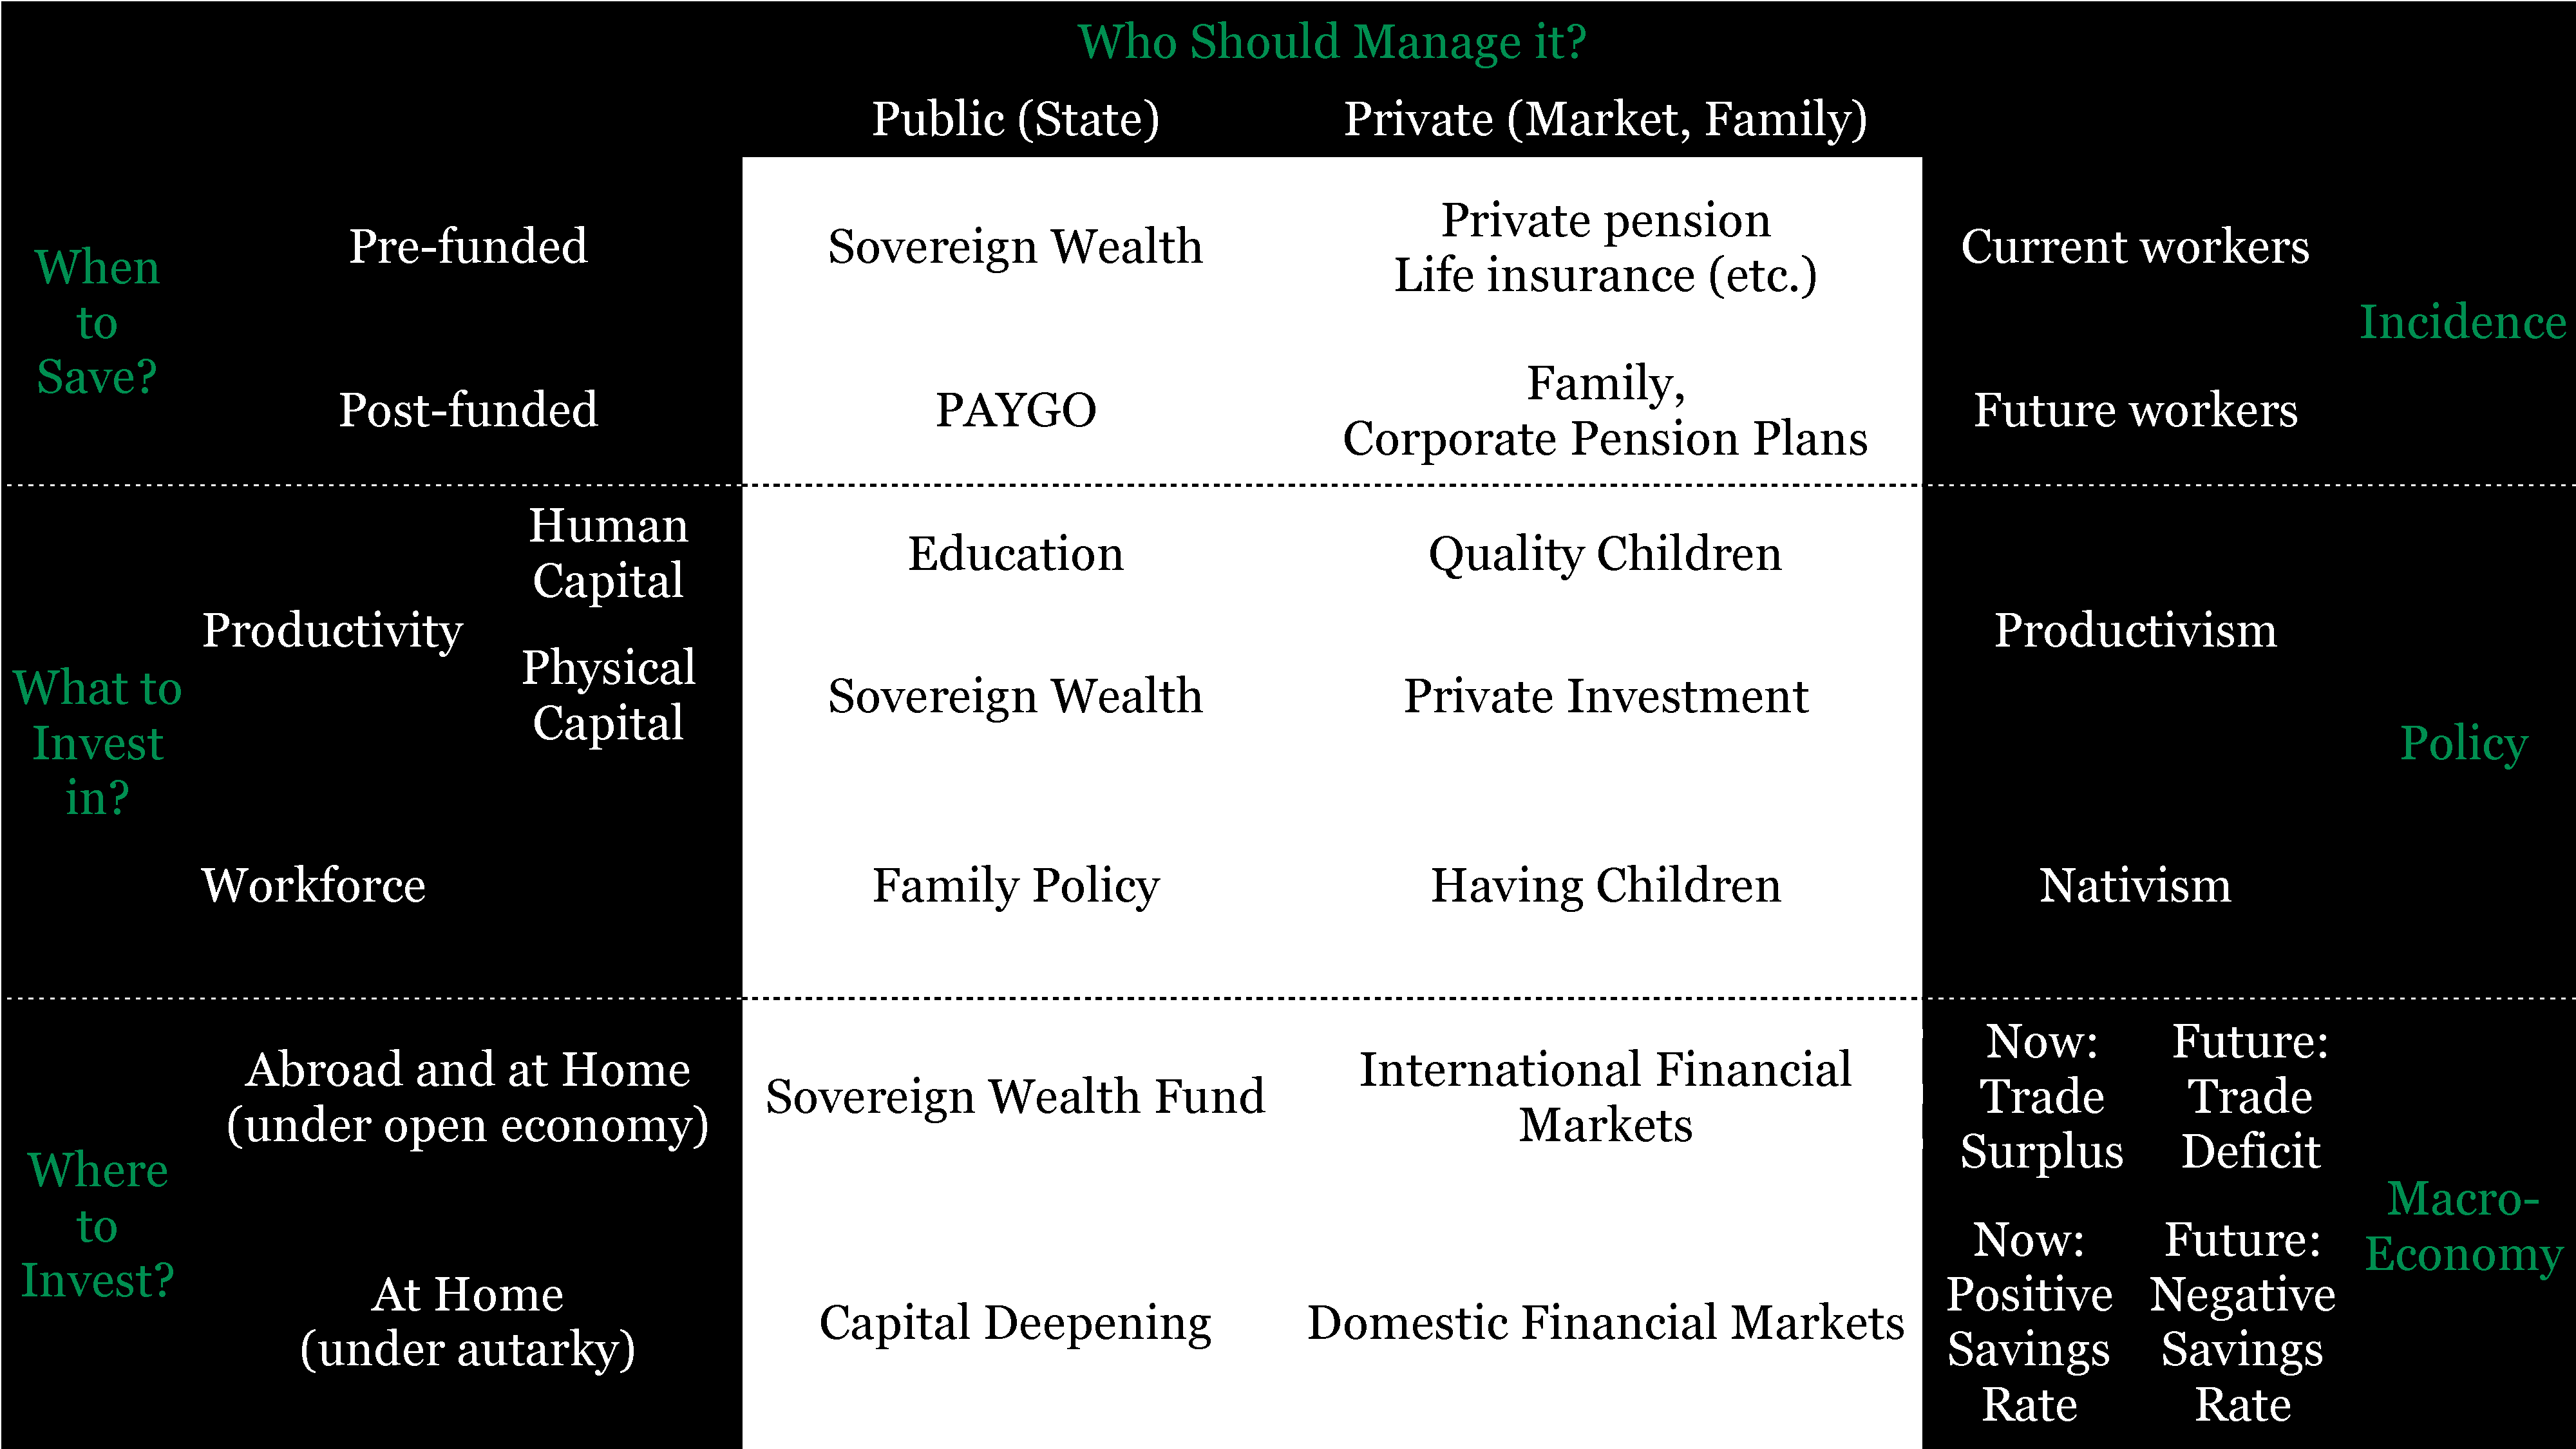
\includegraphics[width=1\linewidth]{pension-design}
	\caption{Pension Design}
	\label{tab:pension-design}
\end{table}%might add family as a third column here.

As summarized in \autoref{tab:pension-design}, all possible pension designs are exhaustively described by tabulating four simple choices:

\begin{description}
	\item[Who Should Manage it?]
	The surplus production saved for old age can either be managed publicly by the state, including its quasi-fiscal institutions, or it can be managed privately by capital markets (see the the middle two columns in \autoref{tab:pension-design}).
	In both cases, savers acquire some kind of ownership claim to the accumulated surplus:
	if under public management, savers own their savings as \emph{entitlements}, governed by public or administrative law, if under private management, savers own their savings as \emph{property}, governed by private law.
	\footnote{
		In \citeauthor{Barr2005a}'s precise formulation, ``PAYGO and funding are both financial mechanisms for organizing claims on that (future) output.
		[\ldots]
		Funded schemes are based on accumulations of financial assets, PAYGO schemes on promises'' \citeyearpar[157]{Barr2005a}.
	}
	\footnote{
		In addition, the right of current savers to future pensions can take the form of \emph{equity} or \emph{debt}.
		As equity, in either private stock or public economy-wide growth, savers partake fully in both the upside and downside risks:
		if either the stock, or the economy as a whole grows or falls, so do their pensions.
		For example, mutual funds share risks under private management and a strict defined-contribution PAYGO-systems share risks under public management.
		As debt, in either private bond markets or entitlements to future economy-wide incomes, savers are insulated from all but the risk of default.
		For example, private life insurance includes only a risk of default, and a strict defined-benefit PAYGO-system --- at least nominally --- carries only the risk of sovereign default.

		In publicly managed pension schemes, the distinction between the risk profile of equity and debt is often muddled, as future, \emph{nominally} defined-benefit returns are sometimes partly indexed to demographic change, labor incomes, inflation, economic growth or other, risky macroeconomic factors.
		If and to the extent that such pension schemes turn out to burden future pensioners, instead of future taxpayers or ``social insurants'' with the shortfall, they become de-facto equity investments.

		The distinction between equity and debt risk portfolios to publicly managed pension systems carries only so far:
		in contrast to equity in corporations, equity in sovereigns --- at least ideally --- is always ``non-voting stock''.
		Conversely, sovereign defaults are different from corporate defaults:
		in democracies, bondholders \emph{cannot} turn into shareholders and ``take over'' as they would in an insolvent private corporation.
		The default risk of sovereign bonds is qualitatively different:
		if a publicly managed pension scheme defaults on its obligations, pensioners can change policy only in their capacity as voters, but, aside from basic rule of law protection, not in any \emph{additional} capacity as bondholders.
		The bottom line is:
		if push comes to shove, in publicly managed pension schemes, whether you are a shareholder or a bondholder, your power to change outcomes are mostly those of ordinary voters.
	}

	\item[When to Save?]
	Pension schemes can either be pre- or post-funded.

	When they are pre-funded, present surplus production is coagulated into capital \emph{before} future consumption exceeds future incomes in old age.
	On introduction, current workers bear the initial incidence.
	Pre-funded pension schemes can be, for example, managed by the state as \glspl{swf}, or provided by markets as life insurances or other annuities.\\
	When they are post-funded, future income-exceeding consumption in old age is paid out of \emph{future} surplus production of other, younger people.
	On introduction, future workers bear the initial incidence.
	Post-funded pension schemes can be, for example, managed by the state as PAYGO, or provided privately in families, or as corporate pension funds.
	\footnote{
		While practically useful, the distinction between pre- and post-funded is mostly nominal, and does not always, in fact, correspond to real savings quotas of an economy.

		If pre-funded capital is nominally invested in asset bubbles or other overvalued junk, much of the hard-earned surplus production may actually go to waste and coagulate little in the way form of capital that will actually be valuable, or generate a return in the future.

		Conversely, if people are free from such post-funded obligations, but instead use their surplus production to have more children, educate them better, built a home or a company, they \emph{have}, the economy as a whole, does in fact accumulate capital.

		In this sense, the current support for pre-funded schemes is based on a false sense of certainty:
		whether pre-funded pension schemes \emph{actually} stash away enough for old age depends on how good the investments are.
		The next question, of \emph{How to Grow} is therefore a more meaningful choice than the tiresome pre-funded vs.\ post-funded controversy.
	}

	\item[How to Grow?]
	\emph{Any} pension scheme needs to coagulate surplus production somewhere, somehow.
	Excluding exogenous growth, the long-run output of an economy is determined by the size of its workforce, and the productivity of its workers, which is in turn determined by the different forms of coagulated surplus production they command as human or physical capital, or endogenous technology.
	Creating both these drivers of output --- people and their productivity --- is costly.
	The hyper-materialist connotations notwithstanding, creating people or the basis for their productivity are also alternative, competing uses for the surplus of an economy.
	People and economies can use their surplus production to feed a second baby, or to build a room for the first baby (physical capital), or to better educate the first baby (human capital).

	Different pension regimes suggest, and \emph{face} different allocations to generating new workers, and more capital.
	On the public side, a pension regime may invest surplus production --- pre-funded \emph{or} post-funded --- into better education, or a \gls{swf}, hoping that either of those will pay off in increased output in the future.
	Alternatively, a state may try to encourage, and/or individualize the costs and returns of rearing children in its family policy, to increase, or --- better yet --- stabilize future workforces.

	On the private side, a private investment may accumulate into physical capital, or family may pour resources into one prodigious child, hoping that both will increase future productivity.
	Alternatively, a family may decide to have \emph{more} children, hoping that they together, will support the parents in old age.

	\item[Where to Invest?] Lastly, pension schemes can invest their surplus production either abroad and at home under an open economy regime, or, if under autarky, they can invest only at home.
	Crucially, for private markets, the mix between foreign and domestic investments will be determined by expected returns.
	Domestic investment can be enforced only if the economy in question foregoes capital mobility and confines itself to --- at least some --- autarky.

	These investment choices reflect in macroeconomic movements.
	A pension scheme investing heavily abroad will first bring a trade surplus, and later, a trade deficit, both set off by respective flows in the capital account.
	A pension scheme investing only at home will not alter trade balances, but will first build positive savings rates, and later negative savings rates, as the pensions are paid out and consumed away.
\end{description}

%add somewhere a good visualization about pensions, to illustrate the trivial difference between PAYGO and funded.
%Go back to Barr to figure this out, he's got some good ideas.
%There's a box in Barr with the economics of pensions that I should look into.

Each of these choices has to be considered very carefully.
To name just a few of such vexing considerations, private management might help capital markets mature, and contribute to growth \citep[for example][155]{Barr2005a} --- \emph{or} it might help inflate bubbles, and expose individuals to undue risk.
Nativist policy may be considered illiberal, \emph{or} raising children may be considered a positive externality for which parents should be compensated.
Investing pensions abroad may be thought to spur growth and convergence, \emph{or} we might find find the colossal --- if ideally only temporary --- trade imbalances unacceptable.
\footnote{
	Private, pre-funded pension schemes in rich, open economies may cause much capital to flow abroad into emerging economies, where they promise to generate higher marginal returns.
	In the future, these formerly trade surplus, aging economies such as Germany would then run colossal trade deficits with emerging economies such as Brasil.
	While many advocate such a scenario \citep[for example,][176]{Borsch-Supan2003}, I have not read any one remarking on whether such a scenario in which, for example, young Brazilians do much of the producing, and old Germans do much of the consuming would even be conceivable, let alone desirable.
}

The devil, here, as always in policy, dwells in the details, and must be engaged.
I allow myself the rather superficial summary in \autoref{tab:pension-design}, because I want to draw attention to the fundamental equivalences of these seemingly dramatic choices:
however they answer these questions, pension regimes, as all policy, cannot escape the constraints of Haig-Simons, summarized in \autoref{fig:haig-simons-individual-collective}.
If, other things equal, you have fewer children and lower the production of future workers, as Germany presently does, but wish to maintain the standard of living of a future, older Germany and future, older citizens, you \emph{must} invest in either human or physical capital, in some form, by some mean.
If,  other things equal, you cut public pension contributions, you have to increase privately managed saving.

The Haig-Simon identity and, as one of its terms, demographic change,
\footnote{
	The current, second demographic transition (\citealt{Davis1945}, restated by \citealt{Caldwell-1976-aa}) delivered low, often below-replacement level \glspl{tfr} --- the average number of children a woman would have by age 50 based on the current age-specific fertility rates --- and low mortality, concisely measured as life expectancy at birth (after 6 months).

	US 2009 estimated TFR:\ 2.05 \citep{CIA2009}, Germany 2009 estimated TFR:\ 1.41 \citep{CIA2009}, EU-25 2002 TFR:\ 1.37 \citep[2]{Demeny-2003-aa}.
	Life expectancy at birth for EU-25 is 69 years for males and 78 years for females \citep[2]{Demeny-2003-aa}.
}
are unforgiving and inevitable strictures, akin to the law of conservation of matter.
Population aging,
\footnote{
	Falling fertility and falling mortality lead to two interacting effects:
	the population \emph{shrinks} and \emph{ages}.
	Pure shrinking alone could ideally be welfare neutral on a per-capita basis.
	Such pure shrinking with no ageing component would, however, require \emph{rising} mortality as long as TFR is below-replacement level to offset older, larger cohorts.

	Ageing, or more specifically, a change in the dependency ratio between very young and very old transfer recipients and everyone else, however, is an unavoidable welfare loss.
	Fewer people are available to produce for the consumption of more, older people.
}
as other real dissavings, harbor unavoidable losses in future welfare \citep[for example][152]{Borsch-Supan2003}.
They are also both self-reinforcing:
dissaved capital not only earns no interest, but also no compound interest, unborn babies not only cannot support their parents, but they also will not have babies, themselves.
\footnote{
	Demographic shocks echo on for generations and generations, as for example, 1950s baby boomers procreate in the 1970s, and baby-baby boomers procreate in the 1990s, and so on.
	Population dynamics are so damningly powerful because, as \cite{Malthus1798} knew, it grows geometrically, that is, has an incredibly high ``interest'', and therefore compound interest rate.
}

To these strictures, there really are \emph{no alternatives}, no matter the pension design.
There are, however, very real policy choices of whom to burden with the inevitable welfare loss:
\begin{inparaenum} \item whether, and to which extent to burden current or future workers, \item whether, and to which extent to individualize the material costs and rewards of rearing children, \item whether and to which extent to tie individual contributions to individual benefits, and, most importantly, \item whether and to which extent to alter the incidence of the pension design through redistributive intervention, that is, taxation.
\end{inparaenum}

TINA in the literature on building pension schemes in \gls{ceec} or reforming them elsewhere, takes a peculiar form.
It weighs alternative pension scheme designs, where --- with the exception of devilish details --- there really are no meaningful choices, and neglects those very real choices of burden-sharing that democratic polities have.

\citeauthor{Cerami2009a}, for example, though ever critical of ``neoliberal reforms'', describes extensively the addition of compulsory or voluntary private pensions to \gls{ceec} regimes and cites demographic change and --- unspecified --- ``economic and financial pressures'' (sic!) as partial reasons \citeyearpar[336]{Cerami2009a}.
He seems to forget that the intertemporal Haig-Simons identity of an economy is hardly affected by a privatization of pensions:
sure enough, the incidence changes, but no old age crisis can be averted by privatization.
\cite{Barr2005a}, by contrast, are one of the few authors in the field who --- at least implicitly --- endorse Haig-Simons, and exemplarily, reveals the policy options that TINA would have us ignore:
\begin{quote}
	\emph{``An alternative approach [to parametric adjustments] seeks to finance higher future pension spending by reducing other expenditure.
	One way is to reduce public debt now;
thus governments in the future would spend less on interest repayments, freeing resources for PAYG[O] pensions''.}
	\\*
	--- \citet[152]{Barr2005a}
\end{quote}

\citeauthor{Cerami2009a} asks for a ``new politics of aging'', involving institutions, ideas and power as a new second-order theory of social change \citeyearpar[338]{Cerami2009a}, but, before that, rightly stresses a first-order question:
whether, indeed, ``funded'' (by which he means privately managed, pre-funded) pensions really resolve the (unspecified) ``demographic, economic and financial (sic!) pressures'' supposedly arising under ``PAYGO'' (by which he means publicly managed, post-funded) \citeyearpar[339]{Cerami2009a}.
There are at least three TINAs that \citeauthor{Cerami2009a}'s account of the first-order social choice falls for:

\begin{enumerate}
	\item \citeauthor{Cerami2009a} (and \citealt{Bastian1998}, too) seemingly accept ``funded'' vs.\ ``PAYGO'' as a demographically meaningful alternatives, even though they are clearly not.
	Funded, or more precisely, privately managed, pre-funded pensions may change the \emph{incidence} of aging, by burdening current workers, but they not by virtue of being privately managed alter the economy-wide or even individual, intertemporal Haig-Simons identity \citep[for a detailed model, see][170]{Borsch-Supan2003}.
	Privately managed, pre-funded, just as publicly managed pre- or post-funded regimes may, or may not save enough for the future, and may, or may not invest such surplus production wisely to make up for the dissaving in offspring, and growing life expectancy.
	``Pre-funded'' conveys a false sense of austere security that social scientists should not buy into.

	\item Likewise, \citeauthor{Cerami2009a} cites, without reproach, the arguments for ``pre-funded'' schemes, including supposed higher returns of private investments and breaking of the ``vicious cycle'' of PAYGO.
	Both, again, assume alternatives where there truly are none.

	Privately managed funds may, or may not generate higher returns than equivalent \glspl{swf}.
	Any supposed superior performance of one or the other management requires a specific economic theory to explain it, and empirical evidence to support it, non of which are mentioned here.
	\footnote{
		There may be good, theory-driven, empirically supported reasons for favoring private or public management of pre-funded schemes, but that is part of the messy detail that neither \citeauthor{Cerami2009a} nor I can, or need to discuss here.
	}
	To just mention such supposed superiority of privately-managed funds without explaining why that would be so, is to buy into the unquestioned promises of neoliberal ideology.

	There is also no such thing as a ``vicious cycle'' of PAYGO, where, in \citeauthor{Cerami2009a}'s reading of its opponents, ``current workers are forced to pay for current pensioners'' \citeyearpar[339]{Cerami2009a}.
	True enough, a move from nominally post-funded to nominally pre-funded regimes alters the nominal incidence of demographic change, but that is simply a zero-sum redistribution of the hardship that some group, at some point, has to endure.
	There is nothing particularly self-reinforcing about (nominally post-funded) PAYGO, that would make it ``vicious''.

	A similar notion comes from \cite{Bastian1998}, who, with alarm, reports the rising share of public pension outlays in \gls{ceec} GDP \citeyearpar[69]{Bastian1998}, and cites PAYGO as the ``main reason'' of the fiscal malaise \citeyearpar[69]{Bastian1998}.
	That is of course, rather tautologically, true:
	in a PAYGO system, all other things equal, the public purse absorbs demographic change.
	However, he seems to be unaware that the percentage of pensions, or, equivalently, consumption of elderly people, is entirely \emph{invariant} to the pension design.
	If PAYGO is transformed into a ``funded'' scheme, the same number of old people will, all other things equal, still consume the same percentage of economic output.

	\item Conversely, \citeauthor{Cerami2009a} also glosses over the arguments presented against pre-funded reform.

	He reports caution about the supposed demographic cure-all of pre-funded pensions (339), but again, fails to explain why --- as is in fact correct --- the public or private management, or even nominal pre- or post-funding do not alter the Haig-Simons dissaving at all.

	\citeauthor{Cerami2009a} also cites risks associated with unstable markets (339) as evidence for the prosecution of pre-funded schemes, but apparently relying more on leftist gut-feeling than critical reasoning, fails to explain what the theory and evidence of theses risks would be.
	To be sure, pension schemes should probably spread and thereby minimize risk, but as these messy details go, they are no matter to be mentioned in passing.
	\citeauthor{Cerami2009a} here assumes a possibly non-existing alternative by suggesting that \emph{only} privately managed, pre-funded pension schemes are risky.
	Clearly, publicly-managed, even post-funded pensions also include --- albeit probably smaller
	\footnote{
		\ldots or not, according to \citet[178]{Borsch-Supan2003}
	}
	--- risks:
	an \gls{swf} can make poor investments, and even a social-security PAYGO system by only betting on one class of investment (labor productivity) in one market (the domestic economy) takes on risks.
	\footnote{
		For example, \citeauthor{Cerami2009a} presents 2009 \gls{oecd} reports of 20\% losses in private pension funds as evidence against private management.
		That need not be so:
		\begin{enumerate}
			\item The losses may so far be evident only in balance sheets, and need not ever --- but well may --- materialize in diminished cash flows.
			The depreciated assets may bounce back.
			Well-managed funds will insulate individual pensioners from such short- and medium-term fluctuations.

			\item These same losses, might, absent a private pension scheme, have materialized elsewhere in the economy.
			For example, workers might have invested the windfall in other risky assets.
			Bubbles and crashes are inter temporal bumps in the Haig-Simons identity, and they will always hurt the economy --- as \citet[340]{Cerami2009a} concedes ---, no matter their nominal incidence.
		\end{enumerate}
	}
	Pensions --- as all savings --- always entail some risk:
	whoever manages this pre- or even nominally post-funded surplus production has to decide where it will generate the highest return at an essentially uncertain future point in time.
	As \citeauthor{Barr2005a}, again lucidly, point out:
	``PAYG[O] and funding are both financial mechanisms for organizing claims on that [future] output [\ldots] [and] fare similarly in the face of output shocks.'' \citeyearpar[156]{Barr2005a}.

	But \citeauthor{Cerami2009a} here also ignores an alternative, that in fact may exist:
	well- (or better-)regulated markets that efficiently spread, and thereby minimize risks.
	Especially to a critical social scientists there must be a very good reason to assume that financial markets are \emph{always} unable to spread risk, or, absent such compelling (economic, first-order) reason, the social scientist must suggest (sociological, second-order) reasons why the institutions of financial capitalism underperform in this specific way.
	By not even alerting us to this issue, but by dogmatically assuming financial market failure, \citeauthor{Cerami2009a} --- surely unintentionally --- feeds a particularly backhanded TINA of truly neoliberal hegemony:
	that financial markets --- be they good or bad --- cannot be altered, or, that their failure or success is inevitable, and needs no social scientific explanation.
	\footnote{
		For a fully-fledged Gramscian account of european integration, see \cite{Bieler2002,Bieler2003,Bieler2005}.
	}
	%make sure to mention risk in the above.

	Lastly, as an inverse argument to the ``vicious cycle''-critique of PAYGO, \citeauthor{Cerami2009a} cites the ``double payment'' of current workers as they are transitioned to a pre-funded regime.
	\footnote{
		As a pre-funded, privately managed component replaces, or is added to a nominally post-funded, public managed pension, current workers have to pay twice:
		once into a private account for their old age, and once into a public account fur currently old, PAYGO recipients.
	}
	As the ``vicious cycle'', the ``double payment'' argument is mis-construed:
	there is \emph{nothing} particularly bad, or ``double'' about pre-funded regimes, just as there is nothing ``vicious'' about post-funded regimes.
	The difference between the two is a trivial, zero-sum redistribution of the incidence of demographic change.
	Under PAYGO, depending on parametric configurations, the young and/or the old pay for the dissaved future workforce.
	When pre-funded regimes are added to the mix, but all other things remain equal, only the young pay for demographic change.
	The sum paid, in any event, does not change.
	By framing pension reform as a struggle between the currently young and the currently old, \citeauthor{Cerami2009a} falls for an old ruse:
	\emph{divide et impera}, divide and conquer.
	If we obsess about the mystically ``vicious'' or ``double'', but truly trivial incidence of pre-funded vs.\ nominally post-funded pensions, we loose sight of the bigger redistributive choices of aging societies:
	whether to burden the rich, or the poor, to burden current, or future generations.
\end{enumerate}

It may, again, seem nitpicky, to relentlessly criticize authors as critical as \cite{Cerami2009a} himself, who, after all, only reports arguments frequently presented.
Still, I (nit-)pick on \citeauthor{Cerami2009a}, precisely because he is so far left of neoliberalism, but, I would maintain, not persuasively so.
He rightfully alerts us to the ideological import in pension reform debates \citeyearpar[340]{Cerami2009a}, but penetrates not nearly deep enough into the economic abstractions of pension-design to fully expose the hegemony he correctly suspects.
Whatever the merits of his second-order \emph{explanans} of a new politics of pension reform, he has the first-order \emph{explanandum} wrong:
he assumes economic alternatives where there are none (pre-funded vs.\ post-funded), and neglects other, more relevant choices (financial market reform).

TINA plagues not only the right, but, more deviously, the left, too.
When critical social scientists, as \cite{Cerami2009a}, present only the dogmatic, but shorthanded arguments against neoliberalism (``private pensions are too risky''), their important dissent remains superficial, and will easily brushed aside by more assiduous, if duplicitous, neoliberals.

TINA operates not by straightforwardly denying leftists ``possible, better worlds''.
Rather, TINA is neoliberal and conservative in a roundabout way:
it obfuscates the abstractions through which any such hypothetical, preferable worlds may be glimpsed.
And so, even critics as \citeauthor{Cerami2009a}, inadvertently serve TINA, when they neglect the deep economic abstractions, maybe confusing their neoclassical language and hard choices for the neoliberal doctrine that has so successfully appropriated them.
In pension design, as elsewhere in public policy, a Haig-Simons understanding of the economy helps us to sift through the epiphenomenal debates (``funded'' vs.\ PAYGO), to relegate the complex details (financial markets) to appropriate theory and data, and advance to those choices that our scarce, constrained and material world leaves us to take:
how much we should save for future generations and in which form, and who of us, rich or poor, should contribute how much.
\emph{These} are the real first-order alternatives that a second-order theory as \citeauthor{Cerami2009a}'s must take as a starting point.
All policy and all pension designs, underneath the complex detail and nominal casuistry, make these choices.
My hunch is:
many  current designs and their marginal reforms greatly burden future generations, and present non-rich people, a peculiar choice, that may not even enjoy popular support.

\citeauthor{Schui2009} is right to point out that minimizing the problems of old age insurance to demographic change is latently affirmative:
it distracts us from the possibility to redistribute the fruits of growth and the pains of decline \citeyearpar[147]{Schui2009}.
\footnote{
	\citeauthor{Schui2009}, the orthodox leftist, is of course otherwise hardly moved by the strictures of Haig-Simons.
	Ever the die-hard Keynesian --- or Marxist?\ ---, he always and everywhere assumes a crisis of underconsumption, or, equivalently, excessive overall profits, and seems not to allow even the possibility of material constraints at some exogenously given, only slowly expanding steady state.
}

The enormity of these alternatives can hardly be overstated, especially for \gls{ceec}, where hard-working people often spent old age in abject poverty.
As even the aging economies of Europe \emph{are still growing} over the medium- and long-term on a per-capita basis, we should be able to build a pension regime that, somehow
\footnote{
	Progressive taxation comes to mind.
}
\footnote{
	A pension scheme including, or supplemented by progressive taxation, does not preclude actuarial components in a pension formula.
	As \cite{Barr2005a} helpfully reminds us, working longer may not be such an undue thing to ask, if people live longer, too.
	If people some people like to retire earlier, and others are willing to work longer, we might want to punish and reward them accordingly, while still asking the rich to chip in more for any actuarial increment earned.
	Alternatively, and probably more transparently, the redistributive component can also be organized exclusively through the tax code, with pensions remaining cleanly actuarial.

	Evidently from the summary of the mixed economy in \autoref{tab:ends-mixed-economy} (p.~\pageref{tab:ends-mixed-economy}), if, regrettably, not from all real existing self-ascribed social market economies, asymmetrically known \hyperref{sec:risk}[risk] should be covered by compulsory or state insurance.
	This also includes disabilities that may occur more often in old age, or in some occupations.
	Presently, some pension regimes --- clumsily --- include some form of old-age disability insurance, and debates on extending the age of retirement inevitably bring up the plight of the old construction worker.
	In all of this, I assume that there is extensive, compulsory or state-covered disability insurance.
	When I argue for actuarial pensions, and/or later retirement, I assume that whoever cannot, because of occupational or other disability, work into her older age, should receive benefits out of the disability insurance until she reaches the statutory retirement age.
	If, as seems likely, disability clusters in risky or hard jobs --- such as teaching or construction --- it may even make sense to charge a premium for insuring these jobs, so as to raise the costs of such hazardous labor, and to make it safer or rarer.
}
collects this still increasing economic output, saves enough for our children and disburses enough to our seniors.

If we do not, such criminal neglect of the mixed economy certainly deserves a fair trial, and begs a social scientific explanation.

%barr, for pensions is the benchmark \cite{Barr2005a}

\subsubsection{Pangloss}
	\label{sec:Pangloss}

\begin{quotation}
	\emph{``It is demonstrable'' said he, ``that things cannot be otherwise than they are;
for as all things have been created for some end, they must necessarily be created for the best end.
	Observe, for instance, the nose is formed for spectacles;
therefore we wear spectacles.
	The legs are visibly designed for stockings;
accordingly we wear stockings.
	Stones were made to be hewn and to construct castles;
therefore my lord has a magnificent castle;
for the greatest baron in the province ought to be the best lodged.
	Swine were intended to be eaten;
therefore we eat pork all year round.
And they who assert that everything is right, do not express themselves correctly;
they should say that everything is best.''}
	\\*
	--- Fictional Dr.\ Pangloss in Voltaire's novella \emph{Candide} (\citeyearpar[K125]{Voltaire1759}
\end{quotation}

\paragraph{Second Best.}
Today, maybe one of the clearest Panglossian pronouncements comes under the imposing heading of a \emph{Theory of Second Best}, originally formulated by \cite{Lancaster1956}.
As so many great economic ideas, this one has strayed far from its original form, and interbred with ideology to father many illegitimate --- and sometimes  deformed --- offspring.

In its initial, rigorous formulation, the Theory of Second Best showed formally that if --- as seems likely --- some conditions for the pareto optimality of markets cannot be meet, it might enhance efficiency to allow additional, possibly offsetting deviations from perfect competition elsewhere in the economy.
Rather than to fight all market failures everywhere in isolation (``piecemeal welfare economics'', \citeyearpar[11]{Lancaster1956}, \citeauthor{Lancaster1956} suggested that from a general equilibrium view, there may be less demanding \emph{necessary} conditions that could pareto improve the economy, in addition to the often implausible, \emph{sufficient} conditions of perfect competition \citeyearpar[17]{Lancaster1956}.
\cite{TheEconomist2007} explains it beautifully thus:
if your optimal cookie recipe requires chocolate chips and coconut flakes, but you cannot find the chocolate chips, your (second) best bet may be to bake gingersnap, rather than chocolate chip cookies without chocolate chips.
This is the kind of devilish complexity that I allow myself to ignore here, but that policy makers have to consider:
if, for example, research and development are so prohibitively expensive that we absolutely cannot profitably have more than one manufacturer of wide-body aircraft, our (second) best policy may indeed be to stray further from neoclassical doctrine, and to keep subsidizing \emph{The Boeing Company} and \emph{Airbus SES}, so that we can have at least have ourselves a decent, somewhat competitive, duopoly.
There is nothing Panglossian about such hard choices because, it is, in fact, \emph{materially} impossible to develop dozens of competing wide-body designs.
Because for the social sciences --- as for moral philosophy --- \emph{ought implies can}, the second-best of the subsidized Boeing/Airbus duopoly also needs no social scientific explanation.
This \emph{really} is collateral damage to a worthy cause.

After \citeyear{Lancaster1956}, however, the Theory of Second Best as slowly morphed into a general skepticism of state intervention, it is now name-dropping ``proof'' of its \emph{ipso-facto} futility and serves as welcome absolution for the demise of the mixed economy.
\citeauthor{Wolf1987}(\citeyear{Wolf1987,} \citeyear{Wolf1979}), for example, argued that because governments fail, just as markets do, the second-best response to such market failures may be to just let them be.
You can take this argument to merely logical extremes, and throw out government and democracy altogether.
\cite{Leeson2009}, for instance, wonders whether in some (developing economies) settings, anarchy may not be preferably to predatory statehood, whether, in other words, no state would not be second-better than an inevitably failing government.
\cite{Caplan2007}, in an otherwise thoughtful book, seems to suggest that because voters are so invariably rationally irrational, markets may be second-better than democracy altogether.

This has very little to do with the rigorous argument presented by \citeauthor{Lancaster1956}:
he did, at least in \citeyear{Lancaster1956}, never consider a constrained government, let alone an incapacitated democracy to be grounds for ``second-besting'', but, instead even seemed to hope for a government and people powerful and wise enough to heed his call.

This is Pangloss at his finest:
if you assume, as modern-day second-besters do, that the very \emph{means} to deliberately get to a better world --- government and democracy --- are inevitably flawed, you can show, with almost hermetic logic, that whatever world we find ourselves in, must be the best of all \emph{possible} worlds.

In that word --- possible --- lies the catch.
Modern-day second-besters assume that, akin to markets and evolution, government and democracy are \emph{aimless} processes that merely aggregate pre-social, more- or less rational self-interest.
If government and democracy are aimless, it follows --- as it does, in fact, follow for markets and evolution --- that any positive results of government and democracy are beyond reproach, and beyond improvement.
Government failures, as monopoly pricing or an appendicitis, are just \emph{facts}.

%Interesting criticism of "more market".
%Do they really create "stronger incentives to both acquire information and 	evluate it rationally" (272)?
%See: financial crisis!
%(Ok, will need to argue this in great care, talk about Keyne's beuaty context.
%There was some state in causing the financial crisis.
%Ok, Somin points out that whatever the flaws of markets, market actors may have MORE of an incentive to inform themselves than voters.
%This may be correct.
	%Somin is a naysayer of deliberative democracy.
%A pessimist.
%She doesn't look into the essential innovation of DD!
	%However, this is a deeply broken argument.
%We should decide on first-best, welfare economic grounds which decisions are a subject to democractic rule, and which are not.
%We shouldn't have to factor in the inability of democratic systems in this logic.

Enlightenment, the mother of modern science, did not consider democracy, a merely \emph{positive} affair, but a normative prescription.
\cite{Kant1785} asked us not to ``follow your incentives'', but to ``act only on that maxim through which you can at the same time will that it should become a universal law'' \citeyearpar[Chapter 11]{Kant1785}(\emph{ibid.}.
The US Constitutional Convention in 1787, did not just decide to try out this new \gls{fptp} way to aggregate preferences, but ``We the People'' were to do so ``in Order to form a more perfect Union''.
In a free society, social scientists need not believe in these, or any other ideas, but if they reject them all, they deserve not the air of scientific sophistication in which they cloak their utter cynicism.
As mere accountants of the status quo, their work is anathema to Enlightenment, and they ought to be disowned of the emancipatory heritage that the social sciences were endowed with.

But ignoring, for now, the enlightened humanism that comes part and parcel with the social sciences, the logic of modern-day second-besters is also simply fallacious.
Even if government and democracy turn out to inevitably disappoint, such flaws are \emph{not}, to the social scientist, quasi-material constraints.
Because government and democracy \emph{are} the subject matter for the social scientist, she must not presume, but has to \emph{explain} them.
If we do, as the second-besters, exclude from the first-order alternatives to be explained by second-order theory, those alternatives that the political process \emph{may} corrupt, we have thereby conflated first and second-order theory.
Whatever second-order theory might have to tell us about a corrupted political process, we would never learn, if we did not test for the absence of first-best solutions.
This Frankenstein variant of the Theory of Second Best confuses, as \cite{Brubaker-2002-aa} succinctly criticized the literature about ethnic conflict, the ``empirical data'' with our ``analytical toolkit'':
government failure is ``what we want to explain, not what we want to explain things \emph{with}'' \citeyearpar[165, emphasis in original]{Brubaker-2002-aa}.
%add caveat to this, excusing the guy on development second best that indeed, government failure may be endemic under some constellations.

Panglossian bastards of the Theory of Second Best also roam the literature on European and \gls{ceec} welfare states.
I will here only cite one model student of Pangloss', and eminent social scientist, \citeauthor{Moravcsik-2002-aa}, who refutes a supposed neoliberal bias of european integration thus:

\begin{quote}
	\emph{``No responsible analyst believes that current individual social welfare entitlements can be maintained in the face of these [postindustrial, demographic, etc.] shifts.
	In this context, the neo-liberal bias of the \gls{eu}, if it exists, is justified by the social welfarist bias of current national policies [\ldots].''}
	\\*
	--- \citet[618]{Moravcsik-2002-aa}
\end{quote}
%add here

In other words, even if European integration constrained national, democratically governed mixed economies, that would be for the better because these welfare states are too spendthrift to begin with.
Also, according to \citeauthor{Moravcsik-2002-aa}, to suggest that mixed economies might --- using efficient fiscal, regulatory and monetary tools --- alter market allocations any which way they want, is \emph{irresponsible}.
Pangloss would probably applaud how elegantly \citeauthor{Moravcsik-2002-aa} defines away all redistributive considerations, and, for good measure, adds an ad hominem.

\paragraph{En- or Retrenchment.}
Todays Pangloss has grown more sophisticated since the times of Enlightened Absolutism, when he was easy game for satirist Voltaire.
As any influential teacher, he has learned to lead on his students by making them ask the questions that suit his lesson plan.
The lesson relevant here is that on European and \gls{ceec} welfare states.
It is remarkable just what kind of feeble questions our ever-affirmative teacher Pangloss has gotten us to ask.

\cite{Beckfield2006}, for instance, contents himself to ask how much of \gls{eu}-15 income inequality can be explained by regional political integration as opposed to (economic) globalization, and, alarmed, finds that nearly half of it can be explained thus.
He lists the ways in which  regional political integration constrains the welfare state:
through
\begin{inparaenum}
	\item policy feedback such as austerity-enforcing nominal convergence criteria,
	\item diffused classical-liberal policy scripts
	\item possible blame avoidance and
	\item by tying \gls{ms} economic fortunes to one another.
\end{inparaenum}
This is rigorous empirical work, albeit, lacking a natural experiment, and plagued by questionable external validity and --- one fears --- intricate multicollinearity, it will always remain vulnerable to methodological critique.
More important, though, is what \citeauthor{Beckfield2006}, in his quest to tell apart the inequality of globalization and political integration, \emph{does not ask}:
how much of the rising income equality could an intact, european mixed economy have enforced, and why did it not do so?
The bigger question, I would maintain, is what \emph{kind} of political integration could have curbed inequality.
\citeauthor{Beckfield2006}, again, surely is one of the authors rightfully critical of globalization and the current mode of \gls{eu} integration.
Still, Pangloss, one imagines, sympathetically smiles at this diligent student, hardly moved in his affirmation of the status quo by such timid and naive questions.
Pangloss can rest assured, as long as \citeauthor{Beckfield2006} and others busy themselves with the nitty-gritty of welfare state retrenchment, nicely playing globalization off against regional integration, which are really two sides of the same coin.
Ever affirmative, if pressed for an explanation, Pangloss can still wring his hands at the inequality, shrug his shoulders and point to the gains from trade.
He has already won this game, as \citeauthor{Galbraith2002a} wryly observes:
``So what are the facts [of inequality]?
Has globalization hurt or helped?
Oddly, researchers do not know;
mostly they do not ask.'' (\citealt[11]{Galbraith2002a}, also \citealt[158]{Crouch2004}).

If sceptics as \citeauthor{Beckfield2006} are the slightly recalcitrant, but still manageable students in Pangloss' classroom, the naysayers of retrenchment as \cite{Swank-2005-aa} are his overzealous disciples.
\citeauthor{Swank-2005-aa} argues that globalization did not force welfare states to retrench, because, evidently, income replacement rates in unemployment, health and pension insurance remain high.
Pangloss would surely applaud in delight:
``excellent work, all is well!''.
What did \citeauthor{Swank-2005-aa} \emph{not} ask, that would so endear himself to Pangloss?
Plenty.
\begin{enumerate}
	\item Obviously, and at minimum, \citeauthor{Swank-2005-aa} should look at public debt and other \hyperref[sec:smoke-n-mirrors]{smokes and mirrors} of the mixed economy to make sure that these sustained income replacement rates are not built on a base of sand, long washed out by tax competition (p.~\pageref{sec:smoke-n-mirrors}).
	He is certainly right that there will be substantial political pressure to maintain welfare states, but their victories may be pyrrhic if bought at the price of sovereign default, or heightened \glspl{dwl}.

	\item More fundamentally, the causal rejection (!) of welfare entrenchment through globalization as put forward by the optimists needs careful positivist research design.
	This would require a hypothetical, namely a sufficiently large, prosperous and closed economy.
	This does not exist in the OECD world, and may not exist at all in reality, as there is a well acknowledged trade-off between liberalization and prosperity.
	This real world constraint notwithstanding, empirical arguments have to take this methodological problem into account to answer the question whether welfare states can \emph{sustainably} continue to operate under international economic liberalization.

	\item Thirdly, lastly, and most fundamentally, the optimists seem to be not so much optimistic about what a welfare state can do, as they seem to be minimal about what it should do.
	In part, this neoliberal bias follows from an epistemological concentration on the status quo.
	The research question that \citeauthor{Swank-2005-aa}, for example answers, is not whether globalization challenges the welfare state.
	Instead, he argues that it may not affect the status quo of \emph{income replacement}.
	This is an unexplicated, negative and minimal definition of the welfare.
	It assumes that the legislator’s social agenda is limited to income replacement, without regard to broader redistributive issues, particularly the question of who should bear the costs of income replacement.
	More generally put, this amounts to what the public management literature calls an output perspective on how much money is spend on welfare, in this case.
\end{enumerate}

% More generally put, this amounts to what the public management literature calls an output perspective on how much money is spend on welfare, in this case \marginpar{\textsf{(reference)}}.
%Much akin to (absurdly) treating anti-discrimination policy, however extensively defined, as an instance of social policy
%proper \citep{Leibfried-2005-aa}, accepting income replacement as a meaningful dependent variable of welfare retrenchment, reveals the neoliberal bias of this strand of optimistic arguments.
%Income \emph{replacement} already by name, is negatively defined, and diminishes social policy to be concerned with the abolition of negative constraints (hardship from unemployment), of things we cannot do and, at the same time clouds a positive definition of social policy as furthering our freedom \emph{to} do something, not freedom \emph{from} something.

%Welfare regimes are, as \cite{Esping-Andersen-1990-aa} has said, systems of stratification in itself \marginpar{\textsf{(page)}}, and they have been, from the very beginning socialist demands in the 19th century more than epiphenomenal income replacement.
%They are tools to socialize the costs of painful, but welfare-enhancing Schumpeterian \marginpar{\textsf{(reference)}} economic transformations as well as individual hardship and serve as engines to redistribute this very welfare as the legislator wishes.

%\subsection{The Right Hypothetical}

%The indeed quintessential and highly political question for globalization and welfare entrenchment is then, whether the state can still socialize and redistribute as it wants, with no limitations resulting from the behavior of other states.
%Welfare state sustainability then has to be pitted not against past or current performance, but against a hypothetically desired welfare regime under global trade with global redistribution, both within and between countries.

%\subsubsection{The Missing Cell in the Payoff Matrix} In game theoretic terms, to gauge how badly welfare-depressing defection might be, you first have to calculate the payoff of a hypothetical mutual cooperation.

%\begin{table}[htbp]
%  \small
%   \begin{center}
%\begin{tabular}{m{1cm}m{2,3cm}m{2,3cm}m{2,3cm}m{2,3cm}}
%& & \multicolumn{3}{c}{\emph{Rest of World}} \\
%& &Open Markets $\wedge$ High Taxes & Open Markets $\wedge$ Low Taxes & Autarky  $\wedge$ Any Tax \\
%\cline{3-5}
%\multicolumn{1}{c}{\multirow{6}{*}{\emph{Home}}} & \multirow{2}{2,3cm}{Open Markets $\wedge$ High Taxes} & \multicolumn{1}{|r|}{?} & \multicolumn{1}{r|}{$x\geq2$} & \multicolumn{1}{r|}{0}\\
%\multicolumn{1}{c}{} & \multicolumn{1}{c}{}& \multicolumn{1}{|l|}{?} & \multicolumn{1}{l|}{$x\leq2$} & \multicolumn{1}{l|}{0}\\
%\cline{3-5}
%
%\multicolumn{1}{c}{} & \multirow{2}{2,3cm}{Open Markets $\wedge$ Low Taxes} & \multicolumn{1}{|r|}{$x\leq2$} & \multicolumn{1}{r|}{2} & \multicolumn{1}{r|}{0}\\
%\multicolumn{1}{c}{} & \multicolumn{1}{c}{}& \multicolumn{1}{|l|}{$x\geq2$} & \multicolumn{1}{l|}{2} & \multicolumn{1}{l|}{0}\\
%\cline{3-5}
%
%\multicolumn{1}{c}{} & \multirow{2}{2,3cm}{Autarky $\wedge$ Any Tax} & \multicolumn{1}{|r|}{$0< x\geq$ ?} & \multicolumn{1}{r|}{$0< x\geq2$} & \multicolumn{1}{r|}{0}\\
%\multicolumn{1}{c}{} & \multicolumn{1}{c}{}& \multicolumn{1}{|l|}{0} & \multicolumn{1}{l|}{0} & \multicolumn{1}{l|}{0}\\
%\cline{3-5}
%
%\end{tabular}
%\end{center}
%   \scriptsize{The above payoff matrix is not a well-defined, sufficiently formalized game.
%To adequately model the international political economy, \emph{Rest of World}, ROW, would have to be disaggregated into at least two more players, making a two-dimensional representation of the game impossible.
%Liberalization and taxation are impossible to  be adequately modeled with only two players, for then, autarky of one player would by definition imply autarky of the other player.
%In real life, at least theoretically, countries could exit from international trade and finance with other countries still continuing on the road to liberalization.}
%   \caption{A Schematic Payoff Matrix for the International Political Economy of Taxation and Liberalization.}
%   \label{tab:SchematicPayoff}
%\end{table}
%
%\marginpar{\textsf{Quite a bit of thinking, reading is still required for the below.}}
%
%\autoref{tab:SchematicPayoff} shows a schematized payoff matrix of the international political economy of taxation and liberalization\footnote{A number of other qualifications and complications do not feature in this schematic overview.
%The high-vs.-low-tax dichotomy does not take into account the above-mentioned shifts in tax bases and progression, namely to more indirect, regressive taxation which may more closely approximate the actual dynamics of tax competition.
%Likewise, the game between \emph{Home} and \emph{ROW} assumes equal sizes of the two economies and cannot account for differential payoffs depending on country size, that \cite{Dehejia1999} have recently pointed to.}.
%
%\paragraph{You Gain from Trade} Firstly, it assumed here that autarky is always the worst outcome\footnote{The effects of autarky of \emph{Home} on \emph{ROW} crucially depend on the respective sizes of the two economies.
%If \emph{Home} is sufficiently large, it may cause \emph{ROW's} payoff to approximate zero.
%Alternatively, if \emph{Home} is small, its influence on \emph{ROW} will be negligible, and \emph{ROW's} payoff will approximate what it would have been otherwise.
%This result is equivalent to disaggregating the unrealistically uniform actor \emph{ROW} into an n-player game, where the choice for autarky of every single player has a negligible impact on others.}.
%Dynamic effects of protectionism, including infant industry development, are not considered here.
%
%\paragraph{You Lose from Taxation --- Or Not} Secondly, it is assumed, that if one player has relatively lower taxes on open markets, that player will attract same or more factors of production and therefore receive a same or higher payoff.
%The counterparty will receive same or a lower payoff, respectively.
%The empirical picture regarding this payoff is mixed; the above-mentioned optimists seem to suggest that costs of higher taxation --- if they are considered at all --- do not cause significant capital flight \marginpar{\textsf{(references)}}.
%More pessimist analysts suggest, that in fact, relatively higher or more progressive taxation, for example of corporate incomes causes factors of production to move, and thereby payoffs to diminish \cite{Genschel2009} \marginpar{\textsf{(and more references)}}.
%I have therefore assumed that payoffs under higher taxation will diminish or stay same.
%
%\paragraph{Rational Actors Will Play It Safe} Assuming that nothing, not even a probability distribution is known about the outcomes of mutual high taxation, mutual low taxation emerges as a dominant strategy for both players.
%From every other course of action, independent of the behavior of the counterparty, players stand to loose, stay same or receive an unknown payoff.
%Risk-averse actors will converge on mutual low taxation as the Nash Equilibrium.
%
%\paragraph{Empirical Investigation of the Status Quo is Futile} From this analysis emerges a fundamental limitation to empirical investigations of the status quo.
%If we accept that unilateral high taxation will create same or lower payoffs, further assume that that this fact is widely known by rationally acting states, it is logically impossible to gauge whether \emph{in fact}, higher taxation is costly, and if so, by how much.
%For no matter how high these costs are, or whether they in fact would be incurred, we cannot know about them.
%
%The nature of the game is then indeterminate.
%We cannot ascertain from what we observe whether there are gains from cooperation to be harvested.
%We cannot know how much we loose from tax competition, for we cannot see how deep down that putative vicious cycle we already are.
%
%To solve this game, we have to compute a hypothetical payoff for uniform high taxation.
%If that payoff is higher than the currently achieved one --- as is hypothesized here --- and if states behave rationally (!), we then have a strong reason to assume that payoffs for unilateral high taxation are smaller.
%
%Without that hypothetical hypothetical of uniformly high taxation, any attempts to solve the game are marred with a fundamental endogeneity problem.
%
%\subsubsection{Dream \emph{On}, Policy Analyst!}
%
%Even leaving normative considerations aside, as I have tried to demonstrate in the above, just academic rigor alone requires us to hypothesize a hypothetical of a globalized, uniformly taxed world economy.
%
%This certainly requires quite a bit of political imagination, something that political scientists, it appears, like to shy away from.
%The question that economists, political scientists and law students in this field have to answer really is a very basic one that has fallen into disrepute under a misunderstood fetishizing of ``disinterested science''.
%
%Put emphatically, to know whether this world is \emph{the best of all worlds} --- or just why it would not --- a certain amount of dreaming how it \emph{could} be better is not only allowed, but analytically require.
%It is hard to learn just \emph{how much} present conditions constrain us, without assuming them away.
%
%To sum up: explaining why the world is not different (in this, case better), ought to serve the classic Popperian business of disconfirming just as well as showing why it is the way it is, or why it is not worse.

%check this again!
%Not sure about Leibfried!
%!marginpar!
\marginpar{The remainder of this section is still quite confused.
It needs a better structure and I need to double-check the references.
Read with care.}

But Pangloss is pleased with other students, too, including such eminent voices as \cite{Leibfried-2005-aa} who seems to consider anti-discrimination policy as an instance of social policy proper.
Pangloss might silently rejoicing at the neoliberal bias he has so successfully instilled in his student.
Anti-discrimination --- however extensive --- already by name, is negatively defined, and diminishes social policy to be concerned with the abolition of negative constraints, of things we cannot do, of market distortions and at the same time clouds a positive definition of social policy as furthering our freedom \emph{to} do something, not freedom \emph{from} something.

Welfare regimes are, as \cite{Esping-Andersen-1990-aa} has said, systems of stratification in themselves, and they have been, from the very beginning socialist demands in the 19th century more than epiphenomenal income replacement.
They are tools to socialize the costs of painful, but welfare-enhancing \citeauthor{SchumpeterSwedberg-1942-aa}ian economic transformations as well as individual hardship and serve as engines to redistribute this very welfare as the legislator wishes.
The indeed quintessential and highly political question for globalization and welfare entrenchment is then, whether the state can \emph{still} (or ever could) socialize and redistribute as it wants, with no limitations resulting from the behavior of other states.
Welfare state sustainability then has to be pitted not against past or current performance, but against a hypothetically desired welfare regime under global trade with global redistribution, both within and between countries.
In game theoretic terms, to gauge how badly welfare-depressing defection is, you first have to calculate the payoff for mutual cooperation.
In the global context, this certainly requires quite a bit of political imagination, something that political scientists, it appears, like to shy away from.
Even leaving normative considerations aside, in this case, academic rigor alone requires such exercise.

If welfare states can be well or poorly designed mixed economies, achieving different outcomes, we should also judge its prospects by comparing actual or evolving regimes to such hypothetical, but possible and desirable configurations.
That is a very different question than testing whether welfare states en- or retrench, let alone its spurious correlates of income replacement \citep{Swank-2005-aa} or even spending \citep[24]{Kleinman2002}, and a question that would deeply unsettle Pangloss.
As \citeauthor{Offe2003} reminds us:

\begin{quote}
	``The mode in which welfare state institutions change can be explicit reform and retrenchment.
	But it can also be inconspicuous and gradual decay.
	For instance, people may defect from public health and pension systems, trade unions see themselves forced into single-employer concessions bargaining, workers resort to unprotected forms of pseudo self-employment in order to avoid social security dues, if not to illegal (“black”) forms of employment.''
	\\*
	--- \citet[364]{Offe2003}
\end{quote}

\citeauthor{Genschel2005}, too, reminds us of what Pangloss would rather have us forget:
``The effect [of globalization] is not so much to force change upon the tax [and thereby, welfare] state as to reduce its freedom to change." \citeyearpar[53]{Genschel2005}.
This is  why political scientists such as \cite{Pierson2002,Pierson1996} that assume institutional constraints (for example, veto points, \citealt{Tsebelis-2002-aa}) to only work to \emph{prevent} retrenchment, are wrong:
the very same constraints that may prevent or delay nominal cuts will also make it harder for welfare states to \emph{adapt} to, rather than just to recede in the face of changing economic and demographic circumstance.
Nondecision does \emph{not} ``generally favor the welfare state'' \citep[174]{Pierson1996}.
While the welfare state might nominally have retrenched only ``cautiously'' \citep[174]{Pierson1996}, the ground underneath it has shifted, leading to a much graver de-facto change of positions:
it can no longer expand or react, relies on unsustainable deficits or real dissavings and must make do with growing inequality, and sometimes, structural unemployment, non of which \citeauthor{Pierson1996} even mentions.

If we do not inquire about that freedom to change, we will --- as \citet[99]{Kleinman2002} --- eat up the Commission's diagnosis of the european economic malaise:
``the main explanation for the poor unemployment performance of the Community over the past two decades is to be found in the constraints that unresolved distributional conflicts and insufficient structural adjustment placed on macroeconomic policies.''

%In the lesson on welfare state en- or retrenchment we should demand an answer for this question: not only, whether income replacement, or even spending, has declined or stayed stable, but whether mixed economies can still today, as they ideally should, choose arbitrary and efficient mixes of state and market.

To shake off Pangloss, and see clearly the demise of the welfare state, we must ask three new questions, that so far, much of the retrenchment literature has shirked:
\begin{enumerate}
	\item What, \emph{given} a hypothetical, intact mixed economy, would welfare states be capable of, if their democratic sovereigns wanted it?
	This is a question that, absent natural experiments on the matter, cannot be subjected to straightforward positive test, because precisely such a hypothetical, intact mixed economy does not exist.
	Still, we must compare actual to hypothetical regimes, to find out just how constrained actual welfare states may, or may not be, by whichever second-order process we subsequently propose.

	\item What is the highest possible trade-off between equity and efficiency that an intact mixed economy can offer their democratic sovereigns?
	As I have argued in the above, better-designed mixed economies face less harsh --- or even no --- trade-offs between equity and efficiency than worse-designed mixed economies.
	The price for an additional increment of equity in efficiency (or vice versa) not only varies at the margin,
	\footnote{
		It seems reasonable to assume that, akin to a production function with diminishing returns to scale, the relationship will be convex-curvilinear.
		At very low levels of equity, initial improvements in equity will be quite cheap in efficiency.
		At very high levels of equity, further increments in equity might be quite expensive in efficiency.
		At full equity, of course, the free price system ceases to operate.
	}
	but it also varies depending on the set-up of the mixed economy.
	For example, a highly progressive tax on consumption may allow same or greater equity at a much lower price than a compressed tax on labor income.
	\footnote{
		\citeauthor{Offe2003} reminds us that there is no ``hyper-rational'' answer of a \emph{best} balance between efficiency and equity \citeyearpar[445]{Offe2003}:
		that is an essentially political question, and should be decided by democratic sovereigns.
		There are, however, objectively \emph{better} or {worse} institutional designs under which these trade-offs are made.
		For example, experts cannot know an optimal progressivity in a tax code, but they may well show that whichever progressivity the democratic sovereign desires will cost less in efficiency under a consumption than an income tax (for example, \citealt{McCaffery2005}, \citealt{Frank2005})
	}
	More broadly, \citeauthor{Ganssmann2010} has proclaimed the Scandinavian welfare state as the ``winner'' to achieve higher levels of \emph{both} equity and efficiency \citeyearpar[343]{Ganssmann2010}.

	Amongst these higher trade-offs between equity and efficiency, there may, additionally, be local optima of equity-efficiency mixes, complemented by quite distinct institutional constraints and --- somewhat related --- path dependencies, ranging as wide as educational systems and industrial relations.

	I have here mostly ignored these \emph{Varieties of Capitalism} \citep{HallSoskice-2001-aa}
	\footnote{
		At first sight, \glspl{cme} might be considered to be in violation of ordoliberal economic policy, and might therefore be considered incompatible with the largely neoclassical model of the mixed economy I have sketched here.

		This need not be so.

		Straightforwardly, as \citeauthor{HallSoskice-2001-aa} suggest, \glspl{cme} might just have a competitive advantage in the production of incremental improvement, and what appears as deviations from atomistic competition is de-facto firm organization at a higher, economy-wide level --- much as the notion of the ``Deutschland AG'' (Germany Inc.) suggests.
		Akin to the framework suggested by \cite{Hart1990}, \glspl{cme} may simply be an economy's way of minimizing the transaction costs involved in the production of their specialties by ``insourcing'' important counter-parties by institutional design, if not formal merger.
		%compare nature of the firm

		Alternatively, I suspect, many of the institutional peculiarities of \glspl{cme} might be explained --- as I have done here for the welfare state --- as remedies to particular market failures.
		Industry-level wage bargaining, for example, might effectively balance the playing field between monopsony employers and labor cartels (unions).
		Employment protection legislation, conversely, might work to smooth the business cycle (albeit imperfectly) or might insure workers against the risk of specialized education, they might otherwise be to risk-adverse to take \citep[for example,][444]{Offe2003}.
	}
	They, too, are important detail.
	They strongly suggest that there may not be \emph{one} universal mixed economy design, but that quite different designs might coexist and specialize.
	Still, also within \emph{each} of these varieties, there are again different trade-offs between equity and efficiency.
	Interestingly, the institutions that \citeauthor{HallSoskice-2001-aa} identified as markers of \glspl{cme} and \glspl{lme} do \emph{not} mention variants of tax, social insurance or any of the other key welfare state institutions.
	While \glspl{cme} may correlate with, and are often conflated with Bismarckian welfare states, there is nothing about \glspl{cme} that would make them necessarily rely on, for example, labor income-backed social insurance.
	Of course, the variant of capitalism will be reflected in the nitty-gritty of welfare state institutions:
	for example, the statuses originally maintained by Bismarck are, arguably, related to the categorical groups that \gls{cme} educational systems create, or \gls{cme} industrial relations are organized around.
	This institutional spill-over notwithstanding, I would hypothesize, that \glspl{cme} and \glspl{lme} might be able to achieve equally high trade-offs between equity and efficiency, even if the institutional implementation may vary:
	for example, \glspl{cme} might continue to sport extensive job protection, while \glspl{lme} will allow quick ``hire and fire'', potentially complemented by generous unemployment benefits (as in ``flexicurity'').
	Allocative results, either way, may be very similar, which is my point here.

	Even carefully crafted positive research into changing welfare states currently looks, at best, at cross-sectional or longitudinal variation in social transfers as a percentage of output \citep[for example,][249]{Ravenhill2005}.
	This is much better scholarship than the naysayers who like to look only at absolute spending or income replacement, but still, it does not tell us how good a trade-off we are getting.

	To gauge the \emph{level} of trade-off between equity and efficiency available to democratic sovereigns, the retrenchment debate has to look at allocative \emph{results}, not at transfer flows, that is, at inequality (for example, Gini-coefficients) and growth (preferably measures more comprehensive than \gls{gdp}).

	Out of logical necessity, if nothing else, welfare state retrenchment, inequality and growth are \emph{one question}.
	The compartmentalization of these into different academic areas allows not, as one would hope, greater theoretical clarity but instead confuses and waters-down concepts.
	If ``welfare'' is to mean anything, surely, it must be the ability of states to alter allocative \emph{results}, and to do so at a minimum, or democratically acceptable price in efficiency.

	Consider the alternative research designs, that currently predominate.
	If income replacement stays the same \citep{Swank-2005-aa}, but, realistically, incomes become more unequal and states more indebted, is that evidence of a non-retrenched welfare state?
	If transfer volumes rise absolutely, or stay constant relative to output \citep{Ravenhill2005}, but, realistically, ever more people rely on ever smaller transfers, all paid for the labor-incomes of an already squeezed middle class, is that evidence of a non-retrenched welfare state?
	Surely, just external validity requires more extensive operationalizations.
	The best, theory-driven operationalization of a non-retrenched, welfare state is the intact mixed economy.

	\item How well does the welfare state work as an entire system of production and distribution, that is, as a mixed economy?
	This is a very different question from those based on a traditional, more limited definition of the welfare.

	\citeauthor{Offe2003}, for instance, takes pains to remind readers that welfare states have nothing to do ``with equality of outcomes', neither normatively nor positively'', that ``the guiding principle of principle (\ldots) is the security and protection of workers, not equality'' \citeyearpar[450]{Offe2003}.
	This is a historically accurate definition, but it is no longer an externally valid conceptualization of welfare states, if the term is to be more than an empty hull devoid of positive reality and economic possibility.
	``Welfare states as worker protection'' is not \gls{mece} any more.
	By this definition, an economy, or rather, sectors thereof would be classified as a ``welfare state'', in which poorly qualified workers are nominally protected, but either structurally unemployed because their gross wages are higher than their productivity, or live in working poverty, ever unable to participate in the riches of the wider economy.
	To the people working in cleaning or security in Germany today, such a definition would not have a lot of face validity.
	The labor market for poorly qualified workers in Germany is then, at the same time, evidence of a welfare state and evidence of a non-welfare state.
	Conversely, by the traditional definition, an economy, or rather a sector thereof with no nominal protection, but generally high compensation and little economic hardship, would be classified as a non-welfare state.
	For example, freelancers in management consulting, earning handsome but unsteady labor (!) incomes, but equipped with enough assets to weather rainy days, surely do not enjoy welfare state protection.
	Still, at face validity, they also do not exactly suffer from Manchester style laissez-faire.
	Under the traditional definition, they reality is neither welfare-state, nor non-welfare state.

	\citeauthor{Offe2003} might, asked about the plight of German cleaners, point to a leak in the ``Keynesian'' roof of full employment, protecting the lower storeys of welfare states.
	Today, full employment is only a necessary, but not a sufficient condition for an intact roof.
	In fact, full employment might always have been merely necessary, and we were just lucky that in the past, all other necessary conditions were mostly met.
	To stay in \citeauthor{Offe2003}'s elegant metaphor, the welfare state house is facing much harsher weather.
	For example, severe crosswinds of rising income inequality (for example, winner-take-all, efficiency wages) diverging factor returns (for example, Stolper-Samuelson trade), threaten to further drive apart the different economic strata making up the house, threatening to tilt the building.
	In addition, international tax competition, but also home-made dysfunctions are eating away at some of the load-bearing walls, putting enormous stress on the few remaining walls and the (already struggling) people making it up.
	If all we care about in this house is whether the roof is still tight against cyclical unemployment, the structure will not stand much longer.
	If the house of the welfare state is to survive the throes of economic transformation, it needs strong cross-beams, to re-balance the load of its stories.
	These cross-beams are progressive redistribution, and we measure their solidity by looking at overall inequality.
	Today, if not always, the ability of a mixed economy to efficiently curb runaway inequality is the \emph{sine qua non} of welfare states, too.

	This is not new to \cite{Offe2003}, who also includes ``monetary, fiscal, trade and economic policies'' in the roof \citeyearpar[543]{Offe2003}.
	However, he seems to neglect that consequently, the different stories of welfare protection \emph{cannot} be organized (financed) irrespective of overall inequality:
	if, for example, the fiscal shingles are to remain intact, the protection schemes must charge those most who can best afford it and in a way that will least affect them.
	\footnote{
		This is also why, at least for welfare state researchers, or those concerned about social integration should not look only at relative, let alone \emph{absolute} poverty (as \citet[1]{Grow2005}, and many others) do:
		that research makes invisible the broader context that created that inequality in the first place, and hides who is paying for the poor relief.
	}

	Surely, Pangloss would already despair over \cite{Offe2003}'s insistence on a full-employment protecting roof.
	But with inequality, we can and should ask him an even harder question that might reveal his unreasonable optimism in starker colors.

	In addition to these functional reasons, there are normative and empirical reasons to demand of welfare states worthy of the label to, at least, be able to curb inequality.
	Normatively, it seems questionable to constrain the surely emancipative agenda that once endowed welfare states to worker protection.
	That's quite little to ask of Pangloss.
	Empirically, we know that people care about \emph{relative} differences in access to resources \citep{Frank2005}, that they suffer from \emph{relative} inequality \citep{Pickett-2009-kx}.
	If we are welfare state researchers and, as humanists, care about the human outcomes of institutions, maybe more than evident at Bismarck's time, today inequality \emph{is} that relevant outcome, even if and to the extent that absolute material security is achieved.
\end{enumerate}

\subsubsection[Newspeak]{Newspeak}
	\label{sec:newspeak}

\begin{quote}
	\emph{``When the general atmosphere is bad, language must suffer.
	[\ldots]
	But if thought corrupts language, language can also corrupt thought.
	A bad usage can spread by tradition and imitation even among people who should and do know better.''}
	\\*
	--- George \citet{Orwell1946}
\end{quote}

Some of the literature on European and \gls{ceec} welfare states suffers, plainly, from bad language, especially when social scientists uncritically adopt the language of policy makers as, again, ``to explain things \emph{with}'' rather than as the thing to be explained, as they should \citep{Brubaker-2002-aa}.
At best, this results in terminology and arguments that are devoid of meaning.
At worst --- if not equivalently --- this results in science signing on to the ideology they are meant to disguise.

%add a sentence (this is from the guy from UCI) on the language.
%What does 'neighborhood", what does "community" imply?
%(not good: neighborHOOD, community implies that there's a locale to this problem)

%Why don't we have it?
	%   * Path Dependency (Institutionalism)
	%   * Suspicion, Successful Failure
	%   * Deliberative vs.\ Pluralist Process

Only the mildest from of sloppy language is when social scientists use \gls{eu} terminology, without questioning whether they deliver as advertised.
%\citeauthor{Dehey2003}, for example, in an otherwise insightful article, seems to imply that \emph{actually}, union structural and cohesion funds would drive convergence (\citeyear{Dehey2003}: 566), when clearly these currently paltry funds offer merely cosmetic redistribution.
Similarly, \citeauthor{Sipos2005} report in a chapter for the World Bank that ``after a period of transition confined more narrowly to poverty relief (\ldots) accession to the \gls{eu} \emph{facilitates} restoration of broader and more active instruments of social inclusion [in \gls{ceec}].'' \citeyearpar[89, emphasis added]{Sipos2005}.
Surely, whichever standard \citeauthor{Sipos2005} of social safety net have in mind here must be quite low, as, compared against the homestead of social policy --- the national mixed economy --- there is nothing much to speak of at the \gls{eu} level.

Likewise, \gls{eu} mumbo-jumbo such as ``cohesion'', ``inclusion'' and ``anti-discrimination'' should always be used with care, and quotation marks.
As \citeauthor{Offe2003} reminds us, these are rhetorical devices, not necessarily actual policy goals \citeyearpar[461]{Offe2003}.
What is worse, they cannot be empirically falsified, nor normatively denied:
how do you ever fail ``cohesion'', who could ever be in favor of ``discrimination''?
These, are, in short, ideological terms, that hermetically seal off any actual policy (or lack thereof) thus labeled from political contestation.

Another favorite in this vein is ``social dialogue'' (for example, \citealt{Durr2009}), exuding harmony, agreeability and general fuzziness.
The choice of dialogue, maybe not just to me, seems to imply that, \emph{really}, if employers and employees --- maybe rich and poor, too?\ --- would only sit around a table and \emph{talk}, everything would be fine.
And who could ever be opposed to talking?
The economics of industrial relations, alas, are very different:
they contain --- dare I say it?\ --- a \emph{zero}-sum element, they know winners and losers.
This is not to say that employers and employees may not \emph{also} find themselves in positive-sum games that they \emph{may} solve to everyone's content.
But if such a cooperation problem is encountered and/or solved, that needs to be explained, and must not be ex-ante assumed, by choice of words.

Terminology familiar to economists --- or rather, \gls{ifi} economists --- can also corrupt language.
``Structural adjustment'' \citep[for example,][19]{Begg2008} is such a false friend.
It sounds like an effortless, mechanical process, one that \emph{wants} to happen.
Surely, an unsuspecting reader might not expect that this usually means mass unemployment, pay cuts, and --- absent an insulating welfare state --- material hardship for many people.
There is to the neoclassical economist, nothing wrong right with such transformations, and maybe they are right.
But we ought to, at least once in every article using the term, explicate clearly what it means:
that some economic activity will no longer occur, or not at the same price or wage as before, that many people will have to retrain, or make do with less.

Again, I want to avoid sounding like a ranting conspiracy-monger, and will therefore illustrate my gripe with Newspeak language on two examples in more depth:

\paragraph{\gls{omc} \& Governance.}
Both the \gls{omc} and governance are heavily en-vogue with social scientists in European and \gls{ceec} welfare states, and, as similarly hyped post-isms, are mostly defined in the negative.
The \gls{omc} is, apparently, \emph{not} closed --- but, one is assured, still methodical --- and somehow, \emph{not} hierarchical.
Governance, too, is mostly \emph{not} state and \emph{not} market.
Whoever came up with these terms might have taken a lesson out of a marketers playbook:
against these new-new things, old-fashioned hierarchy, negotiation or government look instantly passe.

Problems arise, when this newspeak creeps into social science.

Governance for once, as \citeauthor{Jachtenfuchs2001} guardedly criticizes, may be a ``\emph{problematique}'' or an empirical phenomenon, but it is not a theory \citeyearpar[259]{Jachtenfuchs2001}.
For the social scientists, \emph{that} is problematic.
Say about state command and market exchange what you will, but at least we have well-articulated theories about how they operate, grounded in somewhat plausible models of human nature.
Critique, in the social sciences, implies theory.
State and market, because we have (competing) theories on them, we \emph{can} criticize:
we can argue about their functions and dysfunctions, about when best to use them, and how to remedy their respective shortcomings.
As for governance, we do not know.
Caution dictates, that, as long as no plausible theory of such a third mode of rule, production and distribution has been explicated, we might better consider these empirical problematiques as deficient states or markets, or, possibly, hybrids thereof.
Using, for now, these old-fashioned theories does not preclude a later, third, genuinely theorized mode nor, for that matter, necessarily implies that all such deficients or hybrids would deliver bad or no results.

The \gls{omc}, too, is a smoke grenade.
For starters, as \citeauthor{Offe2003} acutely notes, it is a misnomer:
if anything, it ought to be an open method of \emph{cooperation} \citeyearpar[467]{Offe2003}.
Coordination --- as in a \emph{battle of the sexes} game --- implies that the payoff of successfully aligned strategies (far) exceeds the divergent interests that players may have in alternative strategies.
In the paradigmatic couple story, the man prefers sports, the wife likes opera, but both want to spend the evening together.
In an extreme case of a coordination game, such as the decision to drive on the right or left side of the road, there is no divergent interest and the game could be solved, if only players agreed on a \emph{focal} point.
Integrating economies, building welfare states and, most clearly, harmonizing tax or other market interventions are, emphatically, no mere coordination problems.
Here, the divergent interests of alternative strategies, when considered \emph{individually rational}, outweigh the benefits of cooperation.
Overcoming something akin to a prisoner's dilemma of individually set tax rates or social policies would be small accomplishment.
Still, the \gls{omc} blithely assumes it to be a fait-accompli.
To be sure, there \emph{are} non-hierarchical ways to solve \glspl{pd} (originally \citealt{Axelrod1980}), and if we are lucky, \gls{omc} consultations produce such happy resolutions.
But if, in fact, they do, it would be nice to learn just how it happened, rather than to presume it would.
Consider, for example, the thoroughly unsatisfactory conclusion that \citeauthor{Theobald2009} draw, after 19 pages of --- supposed --- theorizing elder care systems in \gls{ceec}:

\begin{quote}
	\emph{``Although the \gls{eu} has undoubtedly gained in importance with regard to social policy in its member states, essential decisions are still made at nation state level and determined by actor constellations within the member states.
	Nonetheless, national policy changes are strongly affected by external factors, including foreign models, transnational expert networks, international organizations and the \gls{eu}.''}
	\\*
	--- \citet[163]{Theobald2009}
\end{quote}

Well, that is good to know.
Who would have guessed?

Good language is not just an intellectual nicety.
Newspeak takes the conflict, material, and politics out of policy, where, for now, we must still suspect it.
``Governance'', in \citeauthor{Jachtenfuchs2001}'s minced words, ``almost completely ignores questions of political power and rule'' \citeyearpar[258]{Jachtenfuchs2001}.
The ``\gls{omc}'' by its suggestion of Potemkin harmonization, is not so different from the ``political'' science that \cite{Agnoli-1989-aa} berated for ``praising a state under careful circumvention of its economic underbelly [\ldots]'' \citeyearpar[195]{Agnoli-1989-aa}.
\footnote{
	In the german original:
	``Lobpreisung einer Staatsform unter sorgfältiger Umgehung ihres ökonomischen Unterleibes [\ldots]'' \citep[195]{Agnoli-1989-aa}.
}

If --- as deliberative democracy (for example, \citealt{Elster-1998-aa}) --- these concepts imply normatively, that policy-making \emph{should} shed such unhappy remnants, they should come out and say it.
If --- as, maybe, behavioral economics (for example, \citealt{Tomasello2009}) --- these concepts indicate positively, that policy-making \emph{does} sometimes occur without the selfish demons of our nature that state and market are out to civilize, they should come out and prove it.

What social scientists must not do, is to add these concepts to the ontology, \emph{under} the radar of contestation.
However much it may pain us post-ideologues to speak of \citeauthor{Agnoli-1989-aa}an underbellies of power and material inequality, that is where ---not just figuratively speaking --- society reproduces itself, and where therefore, we must look.

\subsubsection{Bystanders}

\begin{quotation}
	\emph{``If there is a hard, high wall and an egg that breaks against it, no matter how right the wall or how wrong the egg, I will stand on the side of the egg.
	\\
	Why?
	Because each of us is an egg, a unique soul enclosed in a fragile egg.
	Each of us is confronting a high wall.
	The high wall is the system which forces us to do the things we would not ordinarily see fit to do as individuals.
	[\ldots] We are all human beings, individuals, fragile eggs.
	We have no hope against the wall:
	it's too high, too dark, too cold.
	\\
	To fight the wall, we must join our souls together for warmth, strength.
	We must not let the system control us --- create who we are.
	It is we who created the system.''}
	\\*
	--- Haruki Murakami (Jerusalem, 2009)
\end{quotation}

To me, the most outrageous attitude to take on European integration and \gls{ceec} welfare state is no attitude at all.
Being merely a bystander, for many social scientists, appears not only to be acceptable, but the professional thing to do.
As ``normative'' has become a dirty word in many social science departments, and prescriptions something to snicker at, ``disinterestedness'' now appears the lone, unchallenged criteria for good science.
Somewhere along the way \emph{a} political science (politische Wissenschaft) has turned into \emph{apolitical} science (Politikwissenschaft).

This is evident in much of the literature on European and \gls{ceec} welfare state, that, for the most part, refrain from judgment.
Even eminent scholars in this field now fetishize disinterestedness:
Scharpf asked me in a 2011 e-mail whether ``as a policy researcher, I wanted to work on (a however likely, initiated by whomever) revolution [sic!] or contribute to \emph{real} political decision processes in \emph{real} existing polities'' (emphasis added).
\marginpar{Do not quote or circulate the Scharpf quote.
I have not cleared it with Scharpf.}
%!marginpar
Hemerijck, after a presentation on an alternative tax regime opined that he considered history smarter than himself --- or myself, for that matter.

This science turned ignorant is neither humanist, nor, I would maintain, a worthy heir to the spirit of enlightenment that bore its methods 250 years ago.

The operative metaphors here are that of a bystander or a witness.
Of course, witnesses must not embellish their accounts to suit their ideology, or theory:
as far as possible, they should report only the facts.
Also, witnesses must not take the law in their own hands:
passing judgment is up to the judges.
This code holds for social scientists, too:
they should not cook the data to suit their theory, or, present facts that cannot be falsified.
Social scientists, too, are not philosopher kings, or guardians:
the democratic sovereigns, not the professors, call the shots.

Still, a witness bears a responsibility:
to alert others to the injustice she has observed.
Social scientists, are, whether they like it or not, often the lone expert witnesses on a scene.
In our modern, complex world, there will, increasingly, be no one else to sound the alarm.
Take the demise of \gls{ceec} welfare states for an example:
who, if not the social scientists should alert the wider public that \emph{other welfare states} are possible?
Only social scientists and economists can conceive of better designed mixed economies and blow the whistle:
``\emph{no}'', they should shout, the hardship and instability suffered by the people of \gls{ceec} is not materially inevitable, it is a particular choice made by particular people.

Pointing to the alternatives to the status quo does not, as many seem to fear, taint all empirical research.
There are still plenty of entirely positive questions, for example, how to best organize a public service such as waste disposal.
Social scientists as witnesses need not and should not have a position on this:
it is \emph{not} a normative, but a positive question.
They can test which kind of observed, real existing and hypothetical, reasonably imagined way of waste collection is more efficient or equitable.
Once that work is done, social scientists can compare reality to what they know is possible, and inform people about the difference and why it exists.
To simply note that, apparently, waste disposal was privatized because city budgets were tight, however, is to not bear witness, but to be a bystander.

Because so many of the other people on the crime scene have never learned what is positively possible, and what not, they will often be unsure about whether a particular event was man-made or materially inevitable.
For that reason, they need first, economists to clarify what is possible in a scarce world, and second, social scientists to explain why and how the man-made events were made.

This is not a new thing to ask of social scientists.
Proponents of public sociology (Gans 1988), and, before that, \citeauthor{Mills-1959-aa}'s call for sociological imagination meant exactly this:
%gans citation missing
to, true to their emancipatory heritage as science, \emph{enlighten} fellow human beings about the abstractions and alternatives facing the modern world.

It is particularly important in the realm of welfare state design in Europe, and the suffering \gls{ceec}, where the relevant abstractions and alternatives are vanishing into oblivion, and are being replaced by ideology-infused newspeak, ever-optimist Panglosses and depoliticized TINAs.
To do meaningful second-order, sociological or political science work on the welfare state, you first have to do some first-order, economic work, if nothing else, because it lets us talk about welfare as if people mattered:

\begin{quote}
	\emph{``In the first instance, we are interested in the welfare state because we are interested in human welfare.''}
	\\*
	--- \citet*[236]{Haggard2009}
\end{quote}

%from Unger, via wikipedia on Social sciences and humanities today
	%Unger thus sees that the state of the social sciences and humanities today have succumbed to the sway of three impulses that stagnate their development and curtail their transformative power.These are the rationalizing, humanizing, and escapist impulses.
	%Rationalization: contemporary social scientists rationalize the present social order as a natural state of arrangements and see it as the victor of a competition with failed alternatives.
%In practice, social scientists merely explain why the current institutional landscape is the way it is, without recognizing that the social arrangements under exploration are the product of a particular historical time and place.
%The laws that they generate, therefore, cannot be universal laws for human societies, for once the institutional context changes these "laws" will no longer be valid.[24]
	%Humanization: political and legal thought today operates on the premise that we cannot change society fundamentally and thus should only strive to make humanely better an imperfect world.[25] Rather than restructuring the foundations that cause inequality and insecurity, those that aim to humanize the world advocate compensatory transfers of wealth by governments to attenuate the inequalities and insecurities of the market economy.[26] For Unger, those political and legal theorists that limit themselves to only humanizing the present order suffer from "the poverty of the imagination of structural change" and the false view that we must choose between humanization (reform at the edges) and revolution (the substitution of one whole system for another).[26] In response, Unger argues that one need not choose between revolution and humanization because societies are not "indivisible systems, standing or falling together" and thus we can bring about their piecemeal reconstruction.[24]
	%Escapism merely describes and explores adventures in consciousness, which bear no relation to confronting the problems of and remaking the social order.
%Escapists focus on spiritual adventurism while giving up on the institutions and practices of society.
%In response, Unger argues that some structures are more inviting to change than others, and that one is mistaken to pessimistically believe in a universal maxim that all structures are unchangeable enemies to our transcendent spirits.[27]

	%\subsubsection{Three Taxes, And You're Done}
%Conversely to the above account of the twin crisis, this constitutes a ``best case scenario'' of an hypothesized optimal fiscal configuration.
%Notwithstanding empirical and modeling qualifications, this idealized configuration will serve well as a normatively justified hypothetical to guide a new investigation of the international political economy of tax competition.
%

%see ganghof note 2007: he's dead wrong.
%strong reliance on regressive taxes was conducive to building and maintaning a large welfare state.
%Nope, nope, nope.
%only in the short term, and only at the cost of rising structural unemployment.
	\chapter{Testing the Hypotheticals}
		\label{chap:testing-hypotheticals}
		%!TEX root=../tax-democracy-held.tex

\chapter{Testing the Hypotheticals} \label{chap:testing-hypotheticals}

In the preceding \autoref{part:puzzle}, I have tried to shed some light on the \hyperref[chap:3-crises]{threefold crises of welfare, democracy and equality} in much of the current \gls{OECD}-world (\autoref{chap:3-crises}, p.~\pageref{chap:3-crises}).
The puzzle is now a little clearer:

\begin{enumerate}
	\item
		In spite of unprecendented prosperity, late \gls{OECD} welfare states are less efficient, equitable and sustainable than they could be, because they fall short of an \hyperref[chap:mixed-economy]{ideal mixed economy} (\autoref{chap:mixed-economy}, p.~\pageref{chap:mixed-economy}).
		Among the institutions of the mixed economy, \hyperref[chap:tax-matters]{taxation matters} especially, because it is by far the most effective and efficient tool for government to improve upon, or redistribute market outcomes (\autoref{chap:tax-matters}, p.~\pageref{chap:tax-matters}).
	\item
		Equipped with a deficient mixed economy and suboptimal taxation, democracies are forced to make unnecessarily unattractive trade-offs between efficiency, equity and sustainability, eroding their \emph{output} legitimacy.
		At the same time, the legitimacy of democratic \emph{inputs} may be undermined by a widening gap between the complexity of an advanced (mixed) economy and the simplifying tendencies of electoral democracy.
		Potentially, pluralist democracy may, in part, have fallen victim to the tightly concentrated special interest that late capitalism offers, especially in the field of taxation.

		Taken together, such diminished legitimacy in outputs and inputs, may help explain widely reported dissatisfaction with democratic performance (but not institutions) \citep[for example,][]{Dalton-2004-aa} and contribute to the apparent mismatch between popular opinion and the governing abstractions of the mixed economy.
	\item
		Net of such constrained welfare and confused democracy, material and political equality would suffer.
		A deficient mixed economy and suboptimal taxation would corrode the social contract, by which democratic government should have some ability to redistribute the fruits of non-zero-sum %href
		games borne by the free exchange of state-protected property rights \citep[compare][]{Crouch2004}.
		Offered only unattractive choices, and thoroughly confused about the abstractions of the mixed economy, citizens would be increasingly impotent under the social contract.
		One suspects, especially poor and poorly educated citizens would be effectively disenfranchised from the social contract.
\end{enumerate}

\section{Background}

These are, admittedly, conjectures.
As first order actualities, they are puzzling only if there \emph{are} preferable and possible first-order hypotheticals.

%read
	%http://en.wikipedia.org/wiki/Arrow%27s_impossibility_theorem
	%http://en.wikipedia.org/wiki/Gibbard%E2%80%93Satterthwaite_theorem
	%http://en.wikipedia.org/wiki/Unrestricted_domain
	%http://en.wikipedia.org/wiki/Non-dictatorship
	%http://en.wikipedia.org/wiki/Revelation_principle
	%http://en.wikipedia.org/wiki/Voting_paradox
	%https://en.wikipedia.org/wiki/Independence_of_irrelevant_alternatives
	%https://en.wikipedia.org/wiki/Von_Neumann%E2%80%93Morgenstern_utility_theorem


\subsection{Better Taxation}

In the following \autoref{part:tax} (p.~\pageref{part:tax}) and \autoref{part:democracy} (p.~\pageref{part:democracy}), I show that under liberal-pragmatic axioms and orthodox ontology (\autoref{chap:wanted}, p.~\pageref{chap:wanted}), we could have vastly \hyperref[chap:better-tax]{better tax} and \hyperref[chap:better-democracy]{better democracy}.

Among doable taxes, a \glsfirst{PCT} potentially supplemented by a \glsfirst{NIT}, \glsfirst{LVT} and/or \glsfirst{WT} appears to offer more attractive trade-offs between equity, efficiency and sustainability than the current tax mixes dominated by \glsfirst{VAT}, \glsfirst{PIT} and \glsfirst{Payroll} (see \autoref{fig:ppf-tax-regimes}, p.~\pageref{fig:ppf-tax-regimes}).

%here used to be \ref{fig:ppf-tax-regimes} which is now only in tax-matters

%here used to be \ref{fig:tax-overview}, now only in proposal

\begin{landscape}
 \begin{figure}[htbp]
	\begin{center}
	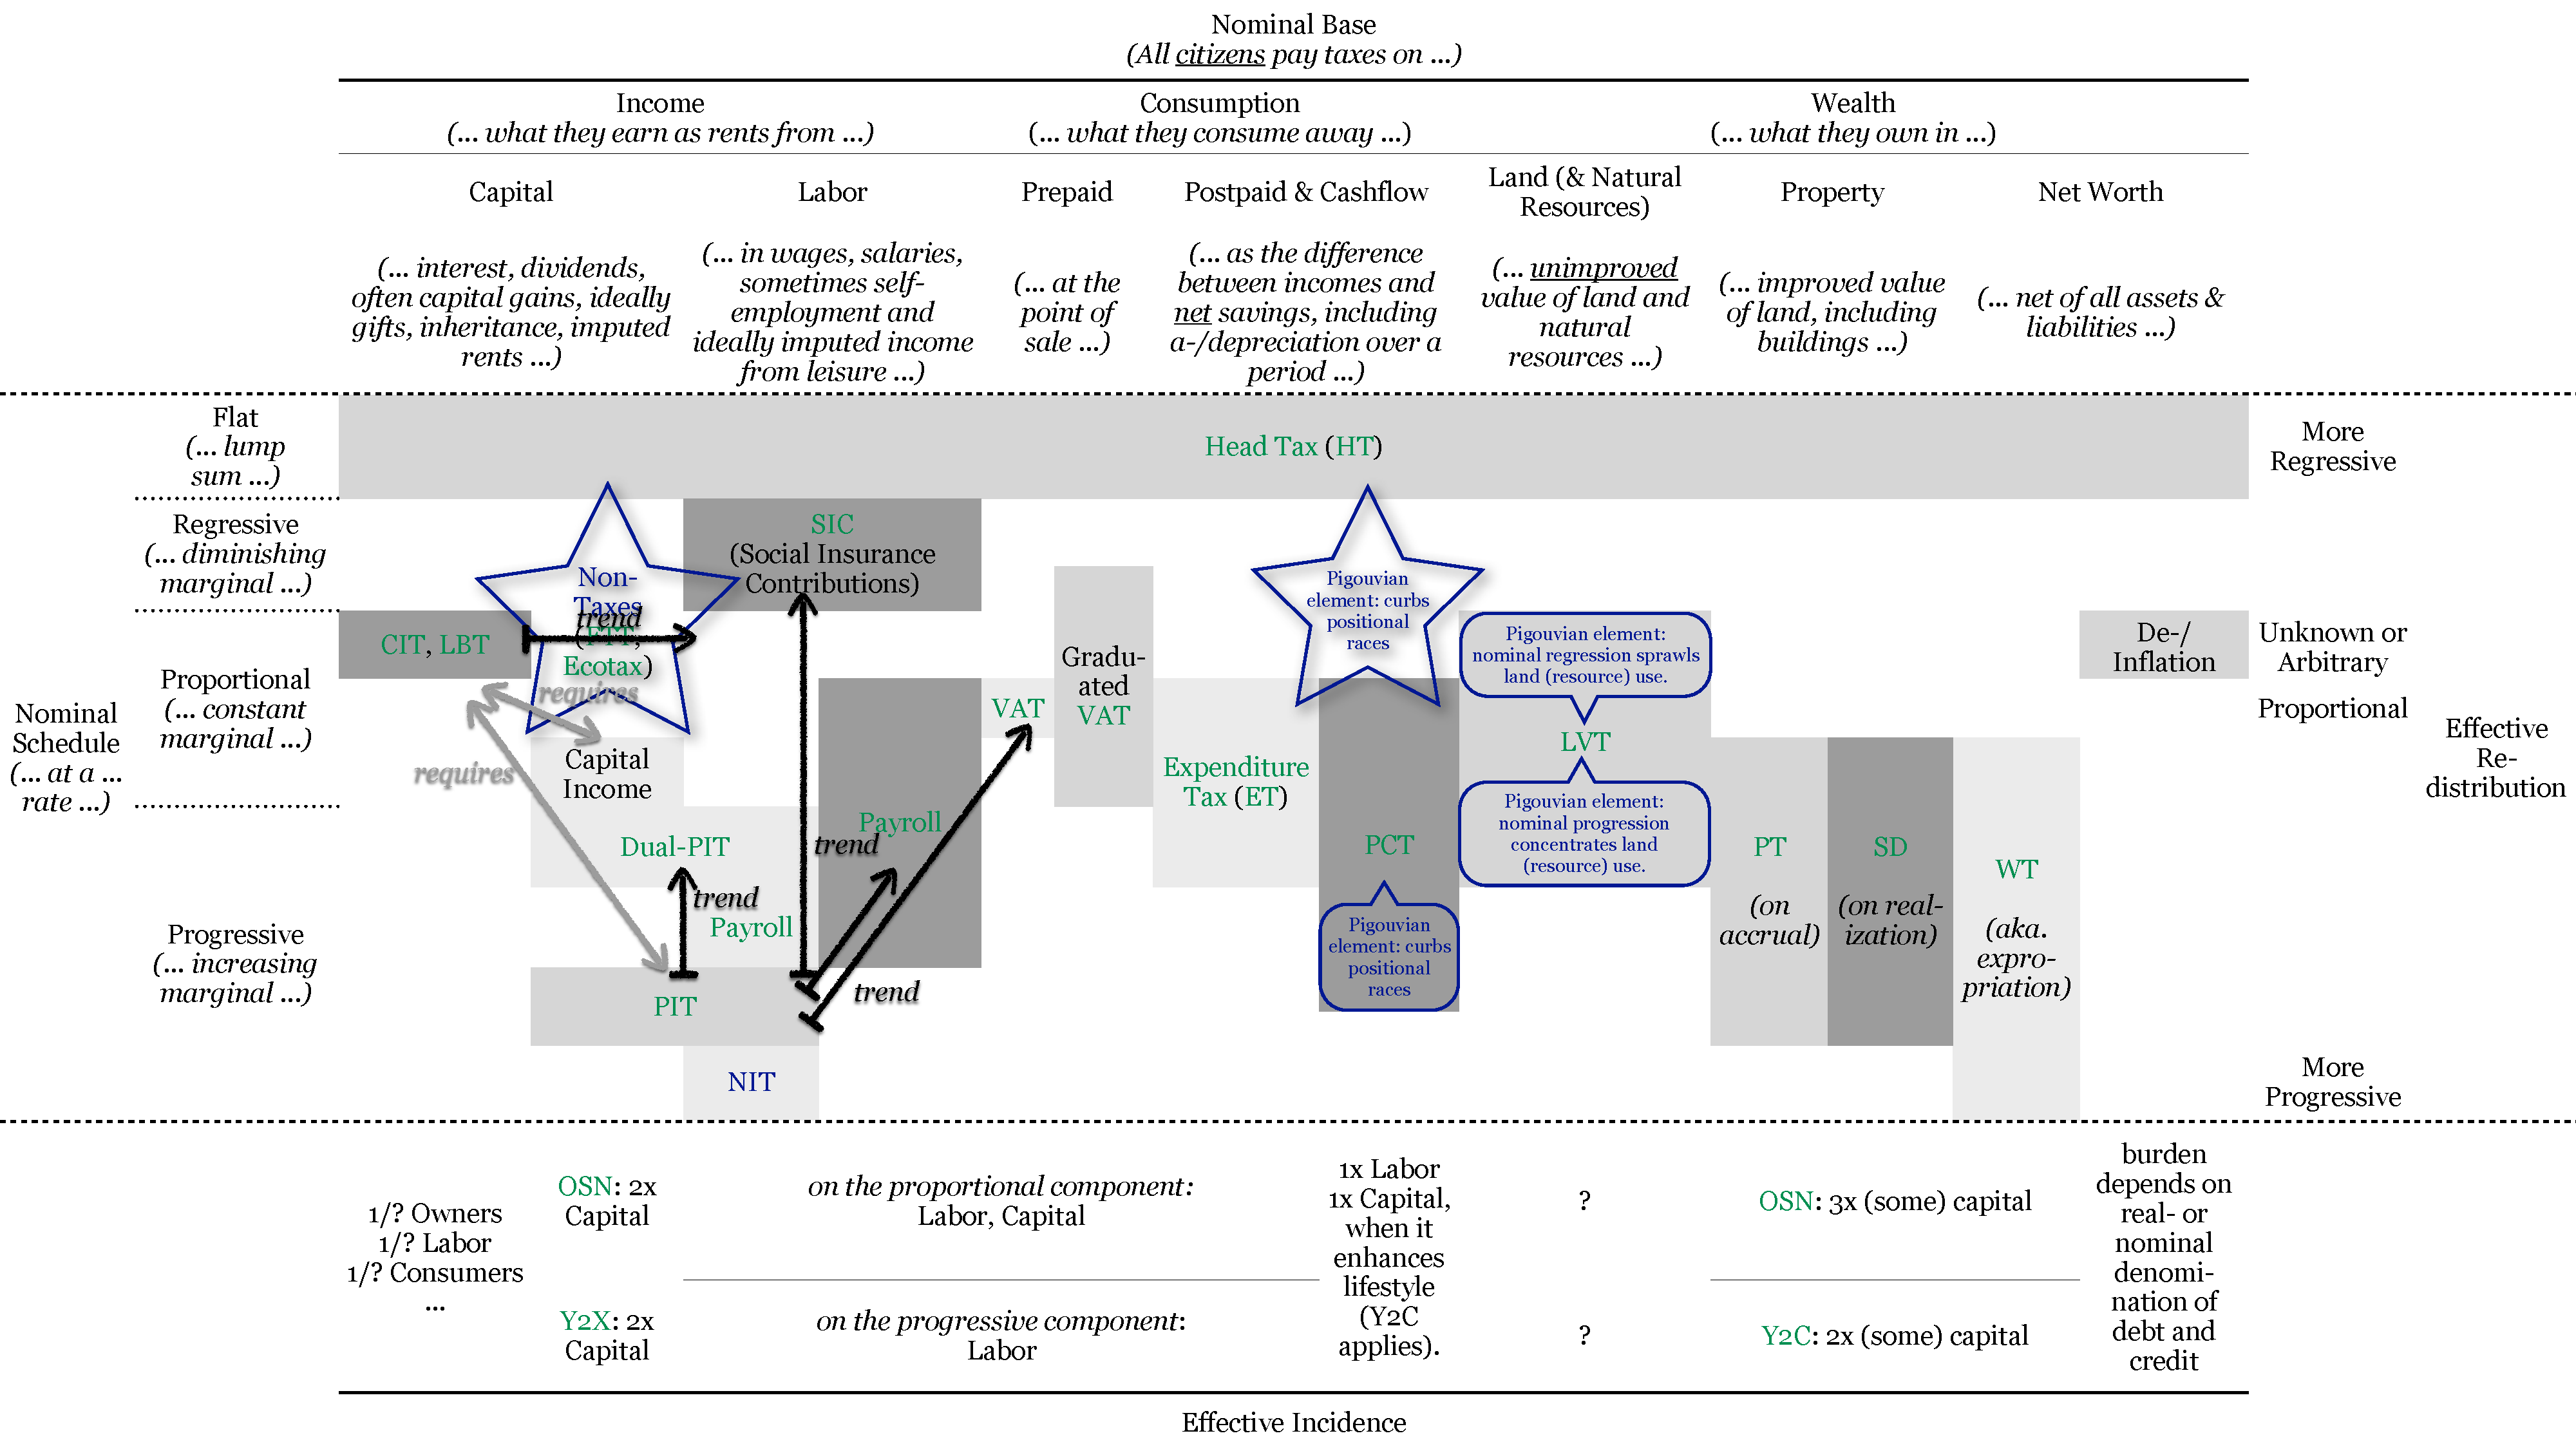
\includegraphics[width=1\linewidth]{tax-with-trends}
	\caption[The Vector Field of Taxes with Trends]{The Vector Field of Taxes with Trends}
	\label{fig:tax-with-trends}
	\end{center}
%	%!TEX root=../tax-democracy-held.tex

\scriptsize{
	\glsfirst{CIT},
	\glsfirst{Dual-PIT},
	\glsfirst{Ecotax},
	\glsfirst{ET},
	\glsfirst{FTT},
	\glsfirst{LBT},
	\glsfirst{LVT},
	\glsfirst{NIT},
	\glsfirst{OSN},
	\glsfirst{PCT},
	\glsfirst{Payroll},
	\glsfirst{PT},
	\glsfirst{SD},
	\glsfirst{VAT},
	\glsfirst{WT},
	\glsfirst{Y2C} and

	\hyperref[sec:distributive-effects-of-inflation]{the distributive effects of in- and deflation} (p.~\pageref{sec:distributive-effects-of-inflation}).
}
\end{figure}
\end{landscape}

\subsection{Better Democracy}

Among doable forms of democratic rule, deliberative democracy \citep[for example,][]{Cohen-1989-aa} appears both more promising and demanding than pluralism.

Deliberation promotes egalitarian, inclusive, well-reasoned and civic-minded discussions for (possibly) consensual political decision-making.
Its normative theory draws heavily on \citeauthor{Habermas-1984}' concept of \emph{communicative action} and \citeauthor{Rawls-1971}' ``Theory of Justice'' as fairness.
Where pluralism encourages the representation of particular interest, deliberative democracy demands \emph{alternative}  conceptions of the common good \citep[18]{Cohen-1989-aa}.
Where pluralism aggregates given, pre-social preferences, deliberative democracy is all about forming preferences.
Where pluralism assumes individual voter error to balance out, when errors are random \citep{Page1993,Surowiecki2004}, deliberative democracy insists on perfecting the deliberators understandings (see \autoref{tab:pluralist-vs-deliberative}, p.~\pageref{tab:pluralist-vs-deliberative}).

%here used to be \ref{tab:pluralist-vs-deliberative}, now only in better democracy
	%it was actually via %!TEX root=../thesis.tex

\begin{table}
	\caption{Pluralist and Deliberative Democracy}
	\label{tab:pluralist-vs-deliberative}
	\small
	\begin{center}
	\begin{tabular}{lcc}
		\toprule 
		 & \emph{Pluralist Democracy} & \emph{Deliberative Democracy}\\
		\midrule
		\emph{Knowledge} & Miracle of Aggregation & Schools of Democracy \\ [10pt]
		\emph{Legitimacy} & Special interest & (Alternative!) Common Good\emph{s} \\ [10pt]
		\emph{Equal Participation} & Representation & Veil of Ignorance \\ [10pt]
		\emph{Speech} & Power & Communicative Action \\ [10pt]
		\emph{Preferences} & Pre-social & Intersubjective\\
		\bottomrule
	\end{tabular}
	\end{center}
\end{table}

Deliberative democracy offers more attractive trade-offs between participation, enlightened understanding and political equality \citep{Fishkin2009} (\autoref{chap:desirable-democracy}, p.~\pageref{chap:desirable-democracy}) and promises to alleviate some of the public choice contradictions of pluralism  \citep[for example,][]{Condorcet1785,Arrow1950} (\autoref{chap:doable-democracy}, p.~\pageref{chap:doable-democracy}).
It also transcends the impoverished, and dubious ontology of pluralism (homo economicus!), and opens legitimate rule to feminist or even virtue ethics.

\subsection{Open Second-Order Questions}

These hypotheticals flow, for the most part, from \emph{a priori} knowledge.
They are grounded in reason, but not --- as hypotheticals can never be --- in \emph{experience}.
I have, as much as possible, supported \emph{a posteriori} assumptions with robust empirical findings --- but I cannot provide  experiential evidence for the complete hypotheticals.

In welfare and tax, comprehensive \emph{a posteriori} knowledge about hypotheticals is hard to come by.

Inframarginal reforms as those I suggest here strain the limits of economic models, all of which must be grounded in only \emph{marginally} known behavioral data.
For example, we would need to know the price elasticity in the demand for luxury goods, or saving and agree on (as I have shown) irreduceably normative judgments of diminishing returns or an optimal savings rate.
%add hrefs
Natural experiments are, of course, unavailable and the external validity of any laboratory setting will be strictly limited.
There is, in other words, not much else beside \emph{a priori} knowledge that we might learn about welfare and tax.
My reasoning here is hopefully as widely agreeable as any comprehensive account of welfare and tax, but it will surely not go uncontested.
Absent empirical clarification, we must then resolve such disagreement in a democratic process.
Taxation, in other words, probably \emph{cannot} be reduced to a first-order question, but it, too reverts to a second-order concern on how to democratically resolve any disagreement we might have about it.
%My topic (tax) is also debated by experts, indeed, experts seem to have the home advantage.
	%But my point is:
%we need to check the work of the experts.
	%ordinary citiznes need to "auf die Finger schauen".
	%We'll see whether the DP or deliberative fora in general can actually do this.

In democracy, we have some, if limited \emph{a posteriori} knowledge about the deliberative hypothetical I here suggest.
Deliberative democracy has been successfully implemented mostly in local settings on policies of limited scope \citep{Fung-2003-ac,HendricksonTucker-2005-aa}.
%not sure this is the right fung reference
In their proposal for ``Empowered Deliberative Democracy'' \citet[17]{FungWright-2001-aa} explicitly suggest what underlies much of the current designs:
\begin{quote}
	\begin{enumerate}
		\item A focus on \emph{specific, tangible} problems
		\item Involvement of \emph{ordinary people} affected by these problems and officials \emph{close} to them
		\item The deliberative development of solutions to \emph{these} problems.
	\end{enumerate}
\end{quote}

Few attempts at deliberating regional issues of greater  complexity have been made, including a `Citizens Assembly' on electoral reform in British Columbia, Canada \citep[confer][]{Ratner-2008-aa}.

On the one hand, deliberative theorists as \citet[17]{FungWright-2001-aa} have criticized this limited scope of deliberative attempts, focused on the immediate, tangible and ``confined to the realm of neighborhood and locale'', as much out of necessity, as out of conviction \citep[759]{Boggs-1997-aa}.
The associated anti-authoritarian, anti-bureaucratic, anti-functional-differentiation impetus may, as \cite{Sousa-Santos-1998-aa} hopes for participatory budgeting in Porto Allegre, Brazil contribute to a ``counterhegemonic globalization'' by concentrating on special issues like land rights, urban infrastructure and drinking water in urban settings, but may by the same token remain ``Bean n' Rice works'' \citep[479]{Sousa-Santos-1998-aa}.
%not the best example, because this is not OECD world
Faced, as our polities inevitably are, with macro-level abstractions, such cherishing of ``human-scale democracy'' above all else may, suspects \citeauthor{Boggs-1997-aa}, move democracy ``in a defensive and insular direction, laying bare a process of conservative retreat beneath a facile rhetoric of grassroots activism'' \citep[759]{Boggs-1997-aa}.
%add somewhere in here:
%an output incongruence arises.

On the other hand, political psychologists as \cite{Rosenberg-2002-aa} have problematized the cognitive demands deliberation poses.
Recent research in political psychology suggests, that --- contrary to the bounded rationality assumption --- imperfect human reasoning may not only stem from remediable cognitive scarcity, but may be developmentally determined.
\citet{Rosenberg-2002-aa} has suggested a threefold developmental sequence and typology of \emph{sequential}, \emph{linear} and \emph{systematic} reasoning.
%add better rosenberg references
His empirical accounts suggest that if any, only systematic thinkers will be able to meet the cognitive demands for reasoned arguments, and egalitarian free speech of deliberative democracy.
Moreover, this cognitive competence was found not to be domain specific, and while people may regress to lower levels of competence under high loads or appropriate cues, they are unlikely to easily, if ever, achieve higher than developed levels.
``Structurally (more and) less developed reasoning adults'' make ``not only the adequacy of citizens' reasoning, but also their \emph{equality}'' a problem for deliberative democracy \citep[12, emphasis added]{Rosenberg-2007-aa}.
%note that the link between rosenbergs sequence thinking and my tax misunderstandings is still to be developed

Few empirical work has been done to address both these ontological and empirical reservations towards deliberative democracy.
We know very little about if and how deliberative fora do in the face of macro-level abstractions and unequally limited cognitive ability of deliberators.

\section{Research Design}

\subsection{Research Questions}

At this intersection of (\gls{PCT}) taxation and (deliberative) democracy, two related research questions arise:
\begin{enumerate}
	\item \label{itm:resolve-better-tax}
		Can democratic rule resolve --- and if so, \emph{how} --- any remaining disagreement about \emph{a priori} desirable and doable taxation?
	\item \label{itm:prove-deliberative-democracy}
		Can deliberative democracy address --- and if so, \emph{how} --- the vastly complex, macro-level abstractions facing our polities?
\end{enumerate}

This dissertation investigates the intersecting set of these two research questions.

In on sense, deliberative democracy serves as the \emph{method} to resolve \emph{a priori} disagreement about taxation, and --- equivalently --- to test whether pluralist democracy may be partly to blame for the absence of better taxation.
Deliberative democracy is a good \emph{method} for research question \ref{itm:resolve-better-tax} on taxation, both because I \emph{axiomatize} it to maximize democratic legitimacy, and I \emph{hypothesize} it to reveal some of the dysfunctions of pluralist aggregation plaguing tax choice (see below).
%note somewhere the public choice fuckup

Conversely, taxation is a good \emph{case} to test deliberative democracy in research question \ref{itm:prove-deliberative-democracy}, because it affects everyone, but is shrewd in the kind of macro-level abstractions which deliberative fora have so far avoided
\footnote{
	For this insight, I am indebted to Franziska Deutsch who first noted in 2011 that tax was an interesting case because it affected everyone, but most people knew little about it.
}
and which may strain the cognitive ability of deliberators.

\subsection{Hypotheses}
Both research questions \ref{itm:resolve-better-tax} and \ref{itm:prove-deliberative-democracy} can be rolled up in one set of hypotheses:

%these hypotheses are gone and now in proposal


%here used to be \ref{fig:tax-with-biases} now only in tax-under-pluralism.tex

%here used to be \ref{fig:tax-with-misunderstandings}, now only in proposal

% \citep[334][]{Farrar2010}
	%The present study examines three important hypotheses about deliberation’s effects.
	%The first is that deliberation frequently alters policy attitudes (continuous dispositions towards policy alternatives) – not only at the individual level (‘gross change’) but in the aggregate (‘net change’).
%The second is that deliberation tends to bring policy preferences (ordinal rankings of policy alternatives) closer to single-peakedness, a help in avoiding cyclical majorities of the sort identified by Condorcet and Arrow.
	%The third is that both these effects tend to be stronger for less salient issues, on which less deliberation has already occurred.
	%Since very few issues are highly salient, these hypotheses together imply an important role for deliberation in shaping majorities and making them meaningful.

	%deliberation helps NOT by brining unanimity, but by changing the structure \citep[2]{List2007}

	%here is something important:
%Condorcet works for pairwise comparisons:
%here we got a problem
	% expanded by arrow:
%ANY voting method must violate one of four attractive properties of pairwise majority voting -- which is why it still matters this problem.
%(Fishkin, etal on meaningful democracy:
%1)
	%violations of independence of irrelevant alternatives open the door to agenda manipulation (Riker 1982), strategic voting (Gibbard 1973, Satterthwaite 1975),

	%deliberation increases ``meta-agreement'' on the dimensions of policy, which, in turn decreases the probability of cycling majorities \citep[9]{List2007}

	%also, say \cite[9]{List2007}:
%these should be the REAL dimensions.

	%\cite{List2007} show that you can get more Condorcet winners this way

	%genschel:
%you show that priming works.

	%social choice (Arrow, Condorcet, Gibbard-Satterthwaite), both in \citep[2]{Dryzek2003} and deliberative democracy

\subsection{Methods}

I test these hypotheses by subjecting people to a \glsfirst{DP}, pioneered by James \cite{Fishkin2009}.
This `Gold Standard' of deliberative fora \citep[55]{Mansbridge2010}, combines skillfully moderated small and plenary group discussions of randomly sampled citizens, rigorously vetted, balanced briefings and experts with pre-treatment, post-treatment and control group opinion surveys into a quasi-experimental design (as in \autoref{fig:deliberative-poll-method}, p.~\pageref{fig:deliberative-poll-method}).

\begin{figure}[htbp]
    \centering
	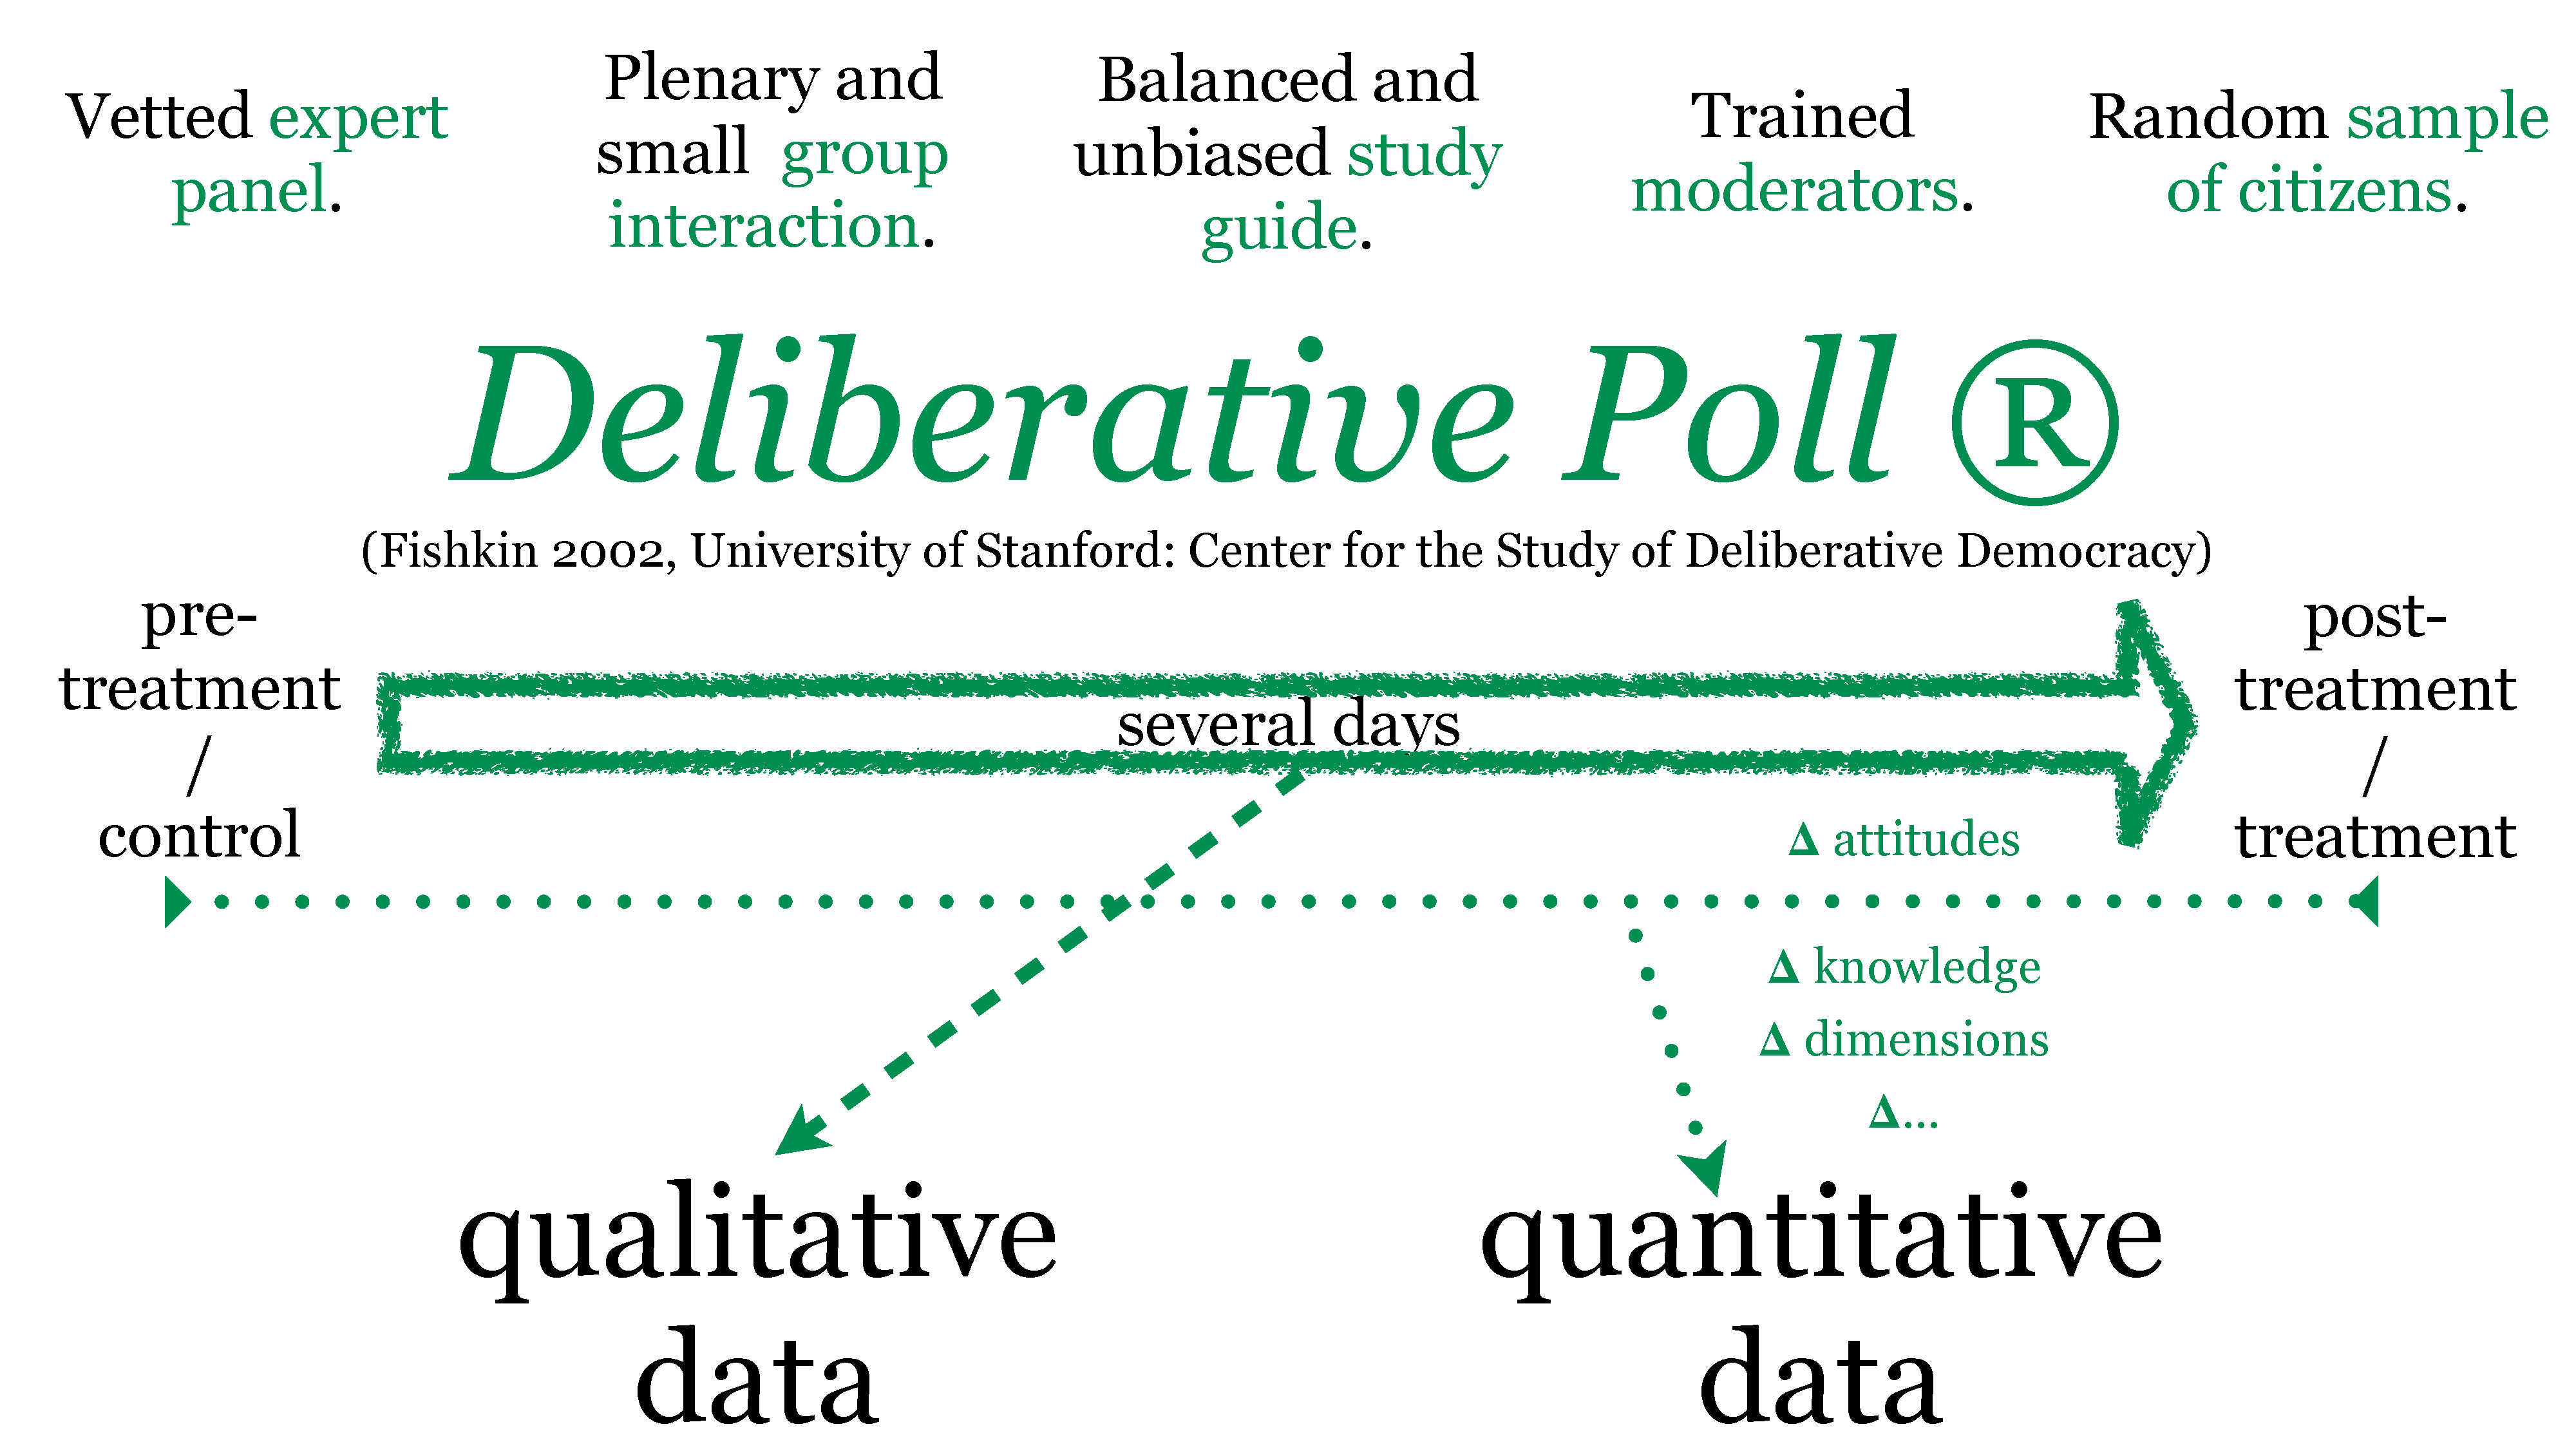
\includegraphics[width=1\linewidth]{deliberative-poll-method}
	\caption{Method of the Deliberative Poll}
	\label{fig:deliberative-poll-method}
\end{figure}

This design suits me well, because it combines the electoral part of democracy with the talking part \citep[308]{ChambersKymlicka2002} and thereby offers the kind of quantitative data needed to test these hypotheses.
Both as a research method and as a second-order hypothetical, it also enjoys high external validity:
it delivers a collective choice and has been shown to work in actual policy making.

	%My thesis investigates this question by qualitatively (discourse analysis?) and quantitatively comparing (survey) the politics (debate) and choice of tax in a status quo pluralist democracy (Germany or the US) with an experimental deliberative forum of ordinary citizens.
	%I hypothesize that ordinary (randomly selected) citizens in a carefully organized deliberative forum will a) think about tax in much greater sophistication, and will b) opt for a PCT regime.

\section{Expected Results}

Hypotheses \ref{itm:knowledge-gain}.x are informed by prior research on the ``Heuristics and Biases in Thinking about Tax'' \citep{McCafferyBaron2003}, supplemented by systematic misunderstandings specific to broad choices between income, consumption and asset taxation.
My hypothesized misunderstandings flow from anecdotal experiences I have had with laypersons and political leaders.
They also shine through in some of the welfare state research, and contrast with my synthesis of an \hyperref[chap:mixed-economy]{ideal mixed economy} (\autoref{chap:mixed-economy}, p.~\pageref{chap:mixed-economy}) and \hyperref[part:tax]{optimal taxation} (\autoref{part:tax}, p.~\pageref{part:tax}).

Hypothesis \ref{itm:attitude-change}, if confirmed, suggests that in fact, remaining \emph{a priori} disagreements about tax \emph{can} be resolved, and that hypothetical taxes really are desirable.

Hypotheses \ref{itm:preference-structuration}.x are related to public choice and opinion research in political science, showing that popular beliefs often violate \gls{vNM}-consistence and can fall prey to aggregation dysfunctions.
Opinions about taxation, in particular, may reveal anomalies at the individual and aggregate level, because tax is highly complex and demands highly structured choices.
Past research has shown that deliberation can alleviate preference structuration anomalies  \citep{Farrar2003}.
A \gls{DP} on tax choice might replicate those findings and extend them to another policy area.

Hypotheses \ref{itm:interaction-effects}.x inform the political psychology, both of tax and of deliberation.
If the above effects do not, in fact, interact with equity beliefs (hypothesis \ref{itm:interact-equity}, tax choice must be affected by something \emph{other} than allocative preferences.
In \autoref{fig:ppf-tax-regimes} (p.~\pageref{fig:ppf-tax-regimes}), equity preferences are moves \emph{along} a curve, and shifts or moves of curves reflect preferences orthogonal to equity.
If, as hypothesized, the above effects do not interact with equity preferences, deliberation may reveal (or bring about) popular understandings in line with the suggested institutional \glsfirst{PPF} of \autoref{chap:wanted} (p.~\pageref{chap:wanted}):
If given some thought, people agree that they can shift the trade-off curve between, say, equity and efficiency outwards, and they prefer those institutions that do.
Hypothesis \ref{itm:interact-ses} is broadly related to the post-democracy thesis \citep{Crouch2004}, by which late \gls{OECD} liberal capitalism and democracy not only disenfranchise the social contract, but do so at a socio-economic gradient.
If confirmed, hypothesis \ref{itm:interact-ses} suggests that under pluralism, people not only prefer taxes less progressive than desired (as per hypothesis \ref{itm:attitude-change}), but that such \emph{false consciousness} is more prevalent amongst people of lower socio-economic status.
The poor (and middle classes) may be too systematically confused to effectively act on their supposed self-interest, reinforcing a mutual crises of political and economic equality.
Lastly, hypothesis \ref{itm:interact-cognitive-ability} is informed by the political psychology of deliberation, and the empirical research on unequal cognitive ability \citep{Rosenberg-2002-aa}.
If, as hypothesized, people with greater cognitive ability will display greater changes along the aforementioned hypotheses, deliberations on tax, too, may have to consider such unequal abilities in their theory and practice.

%		\section[Enlightened Opinions on Tax (or Research Question)]{Enlightened Opinions on Tax \\(or Research Question)}%Research Question

%			\subsection[Conducting Deliberations (or Methods)]{Conducting Deliberations \\ (or Methods)}%Methods

%			\subsection[Witnessing Deliberations (or Data Collection)]{Witnessing Deliberations \\ (or Data Collection)}%Data

%		\section[Misunderstanding Tax (or Hypotheses)]{Misunderstanding Tax \\(or Hypotheses)}%Hypotheses-1

%		\section[Stretching Democracy (more Hypotheses)]{Stretching Democracy \\(more Hypotheses)}%Hypotheses-2

More broadly, a \gls{DP} on tax choice can inform several fields, including research on public finance and the welfare state, public choice and political economy.

\subsection{Public Finance and Welfare State Research}
If the above hypotheses (especially \ref{itm:attitude-change}) are confirmed, welfare research has a lot more to explain.
If under a legitimate democratic process, people resolve remaining \emph{a priori} disagreements to select a \emph{different} tax than we currently observe, welfare state research must provide a second-order theory of the observed (illegitimate) social choice of suboptimal taxation.
I cannot provide, let alone test that second-order theory of tax choice in this dissertation, but --- if hypotheses are confirmed --- can at least suggest that the democratic forum may be important.
Pluralism may not be the \emph{only} reason why we have no better tax, but it might well be one of several reasons.

Political science and sociology have long tried to explain --- if often implicitly --- tax choice.
At least since the fall of Bretton-Woods in 1972, international tax competition has been at the forefront of the academic debate.
In the extreme form, international tax arbitrage is modeled on a \glsfirst{PD} and Nash-equilibrate at low levels and/or proportional schedules as individual countries compete for mobile capital on global markets \citep[for example,][]{Sinn2004}.
%not sure about the source
This extreme form has garnered relatively little empirical support, and has been modified into more nuanced accounts including country sizes \citep{Piatkowski2008,Genschela}, %not sure about the source
domestic politics \citep{Kemmerling2009}, veto playing \citep{Hallerberg2004} and path dependence \citep{Ganghof2009}.
No matter the independent variable, or its configuration, however, all of this research is plagued by a Panglossian unknown:
to explain just which second-order effect has depressed, or altered taxation you must know how it \emph{could} otherwise be.
If successful, this \gls{DP} may reveal exactly such a first-order hypothetical of taxation.
In the language of game theory and pertaining to the tax arbitrage theory, a deliberatively confirmed tax regime of \gls{PCT}, \gls{LVT} or \gls{WT} and \gls{NIT} may constitute the social welfare optimum combination of strategies (High / Open), from which the Nash equilibrium may --- or may not --- differ (\autoref{tab:missing-payoff}, p.~\pageref{tab:missing-payoff}).

\begin{table}[htbp]
  \small
   \begin{center}
\begin{tabular}{m{1cm}m{2,3cm}m{2,3cm}m{2,3cm}m{2,3cm}}
& & \multicolumn{3}{c}{\emph{Rest of World}} \\
& &Open Markets $\wedge$ High Taxes & Open Markets $\wedge$ Low Taxes & Autarky  $\wedge$ Any Tax \\
\cline{3-5}
\multicolumn{1}{c}{\multirow{6}{*}{\emph{Home}}} & \multirow{2}{2,3cm}{Open Markets $\wedge$ High Taxes} & \multicolumn{1}{|r|}{?} & \multicolumn{1}{r|}{$x\geq2$} & \multicolumn{1}{r|}{0}\\
\multicolumn{1}{c}{} & \multicolumn{1}{c}{}& \multicolumn{1}{|l|}{?} & \multicolumn{1}{l|}{$x\leq2$} & \multicolumn{1}{l|}{0}\\
\cline{3-5}

\multicolumn{1}{c}{} & \multirow{2}{2,3cm}{Open Markets $\wedge$ Low Taxes} & \multicolumn{1}{|r|}{$x\leq2$} & \multicolumn{1}{r|}{2} & \multicolumn{1}{r|}{0}\\
\multicolumn{1}{c}{} & \multicolumn{1}{c}{}& \multicolumn{1}{|l|}{$x\geq2$} & \multicolumn{1}{l|}{2} & \multicolumn{1}{l|}{0}\\
\cline{3-5}

\multicolumn{1}{c}{} & \multirow{2}{2,3cm}{Autarky $\wedge$ Any Tax} & \multicolumn{1}{|r|}{$0< x\geq$ ?} & \multicolumn{1}{r|}{$0> x\leq2$} & \multicolumn{1}{r|}{0}\\
\multicolumn{1}{c}{} & \multicolumn{1}{c}{}& \multicolumn{1}{|l|}{0} & \multicolumn{1}{l|}{0} & \multicolumn{1}{l|}{0}\\
\cline{3-5}

\end{tabular}
\end{center}
   \scriptsize{The above payoff matrix is not a well-defined, sufficiently formalized game.
To adequately model the international political economy, \emph{Rest of World}, ROW, would have to be disaggregated into at least two more players, making a two-dimensional representation of the game impossible.
Liberalization and taxation are impossible to  be adequately modeled with only two players, for then, autarky of one player would by definition imply autarky of the other player.
In real life, at least theoretically, countries could exit from international trade and finance with other countries still continuing on the road to liberalization.}
   \caption{A Schematic Payoff Matrix for the International Political Economy of Taxation and Liberalization.}
   \label{tab:missing-payoff}
\end{table}

Other areas of welfare state research may benefit from this hypothetical, too.
As I outline in \autoref{chap:tax-matters} and \autoref{chap:hypotheticals-matter}, optimal taxation and an ideal mixed economy matter a great deal as first-order answers to ask the correct second-order questions.
If --- as hypothesized --- people agree that a \gls{PCT}, \gls{LVT}/\gls{WT} and \gls{NIT} offer more attractive trade-offs between competing values (efficiency, equity), this absence, too is something that welfare state research has to explain.
Here, too, the existing theories rely on such a doable and desirable hypothetical.
The $\Delta$ between that hypothetical and the observed arrangements is a much better dependent variable than spending \citep{Swank-2005-aa} or even decommodification \citep[compare][]{Esping-Andersen-1990-aa}.


%This research informs several fields of \ldots

%	\item{\textbf{International Tax Competition Severely Impairs the Making of Superior Policy}} Specifically, it is hypothesized that indeed --- and counter to the mainstream optimist thesis --- international liberalization \emph{does} restrict the welfare state's ability to redistribute effectively and efficiently (!) as it wishes.
%	\item{\textbf{Veto Playing Matters}} It is hypothesized that veto playing dynamics in particular, and both at the national and international level help explain the suboptimal state of current policy and create a bias for regressive, weak redistribution.
%	\item{\textbf{Tax Harmonization, Development and International Distributive Justice are One}} It is hypothesized that from a careful investigation of the international political economy of tax reform emerges both a political and analytical imperative to think it together with development and international distributive justice.
%Uniformly progressive tax rates on mobile factors of production under the hypothesized hypothetical will crucially affect the chances of developing and emerging markets to capitalize on their comparative advantages.
%\end{description}

%also, hypotheticals are lacking

%Second Order Questions of Social Change
%The second order question of social change is simply:
%Why don’t we have it?
%Possible answers (hypotheses) are:
% Progressive Taxation is subject to an international cooperation problem, akin to a Prisoner’s Dilemma.
%Because the PCT is progressive, it is individually rational for states not to implement it, even if it were collectively rational.
% This is a very interesting question that could potentially greatly enhance our understanding of the international political economy of taxation.
%It however, also requires a comprehensive model of the economy, and even international trade and finance to anticipate the hypothetical payoff of the PCT.
% Tax regimes are subject to great path dependency, they cannot be easily reformed.
% While a historical and tentative analysis of path dependency in tax regimes is possible and probably productive, the costs of reform can ultimately only assessed when a cardinal specification and implementation has been undertaken.
%Assessing the costs of the reform ex ante may be very hard, unreliable or impossible.
%Both a possible international cooperation problem and path dependency in tax regime choice are ultimately endogenous to broader questions of the political economy.
%The cooperation problem depends on the level at which the international political economy is governed.
%Path dependency depends on the domestic and international incidence of reform costs, in turn depending on the states ability to hand out side-payments.

% Ultimately, the PCT could be absent because people do not want it.
%The second order question of social change in tax regimes is:
%will people reject the PCT irrespective of the democratic process that governs their polity?
%If not:
%how do different democratic processes (pluralist, deliberative) constrain or even determine the politics and choice of tax?

%likewise:
%assumed theoretical link:
%if you want to hide injustice, than you'd best do it in a really complex system, like tax.
%
%\subsubsection{Research Question b):
%Why Hasn't it Been Implemented Yet?} Research question b) is then, based on the developed ``perfect tax'', more approximately empirical.
%In the absence of it being implemented in any case, it asks why it has not.
%
%The usual suspect here is a lack of international cooperation.
%Its plausibility will be compared to that of other explanations, namely:
%\marginpar{\textsf{This section needs an overhaul, and \emph{a lot} more reading to make the alternative explanations MECE.}}
%\begin{description}
%	\item{\textbf{Ideology}} Lack of support for such a broadly and boldly redistributive scheme.
%	\item{\textbf{Path Dependency or Historical Institutionalism}} Typological work applies here --- in how far is the tax compatible or not with the institutions and mindsets of established types, for example \cite{BeramendiRueda-2007-aa}.
%	\item{\textbf{Deficient Political Process, Public Deliberation or Discursive Institutionalism}} Literatures on the political process, as well as, on discursive institutionalism \cite{Cerami2009a}.
%	\item{\textbf{International Cooperation Problem}} See above.
%\end{description}

%or addition to science

%First, developed welfare states, in spite of their unprecedented prosperity, appear to be increasingly constrained in their ability to raise revenue and redistribute it as their legislators see fit.
%The pertinent literature on globalization and the welfare state (for an overview see Genschel 2004) asks whether the welfare state has retrenched, and for which reasons.
%Frequently operationalized only as spending (Swank 2005) or decommodification (cf.~Esping-Andersen 1990), that question is incomplete.
%Some of the latently affirmative analyses (Swank 2005) seem to be not so much optimistic about what the welfare state can do, as they seem to be minimal about what it should do:
%income replacement.
%To critically appraise the development of the welfare state, we must instead ask whether legislators are able to raise revenue and redistribute while maintaining growth, factor clearing, low inflation and a positive savings rate.
%We must ask whether legislators were better able to strike this balance of “opportunity and prosperity” (Obama for America, 2007) in the past, or whether there could be a better balance, and then investigate why we do not have better policy.
%Today, welfare states cannot have the cake and eat it.
%They can’t even do one of the two.
%Instead, welfare states are faced with a twin crisis that is mutually reinforcing:
%one of structural unemployment, and one of structural underfunding.
%Structural unemployment is caused by high effective price floors for labor, at or below the socially acceptable minimum income (transfers, minimum wage) in a society, but above the labor productivities of a segment of the workforce.
%Price floors are further raised by an increasingly proportional (or even regressive) tax falling on labor incomes.
%Structural underfunding is caused by a state that is increasingly unable to raise sufficient revenue necessary for the provision of risk pools, public and common goods, as well as to finance its allocative goals.

%Second, my research interest emerges from a sense of utter disconnect between political debate and the abstractions and interests governing the political economy.
%This dis-connect is evident in misleading sloganeering (‘Mehr Netto vom Brutto’, more net out of gross income), widespread superstitions (‘employers [sic!] pay half of social insurance’), bastard Keynesianism (‘consumption is good!’) or redistributive smoke grenades (‘we should tax companies’).
%At a deeper level, I wonder whether pluralist interest and electoral re-presentation can still be reasonably assumed to yield efficient and equitable policies, in an ever more complex world marred by cooperation problems.

%I don't explain the elite-based (potential) reason for the non-reform.
%That, the second-order theory, would be someone elses job.
%discourse theory here?

\subsection{Public Choice and Political Economy}
Public choice has long specified how individual preferences can be aggregated, what it requires and how it can fail \citep[for an overview,][]{Mueller}.
Conversely, (classical?) political economy has formulated theories of how (material?) interest and power can corrupt and alter preference aggregation \citep[for an overview,][]{Robbins1976}.
Both those fields, too, can benefit from deliberating hypothetical taxes.

Public choice, for once, is mostly an \emph{a priori} and often an insular enterprise, merely chronicling --- but not explaining --- the inconsistent preferences and structuration anomalies it faces.
For example, portfolio theory clearly differs from observed loss (not risk!) averse strategies \cite{Kahneman2011}, but we know relatively little about how culture or institutions mediate this gap.
Deliberation is one (possibly attractive!) institution to narrow the gap between \emph{a priori} public choice and \emph{a posteriori} policy preferences.
The hypotheses tested in this \gls{DP} on taxation problematize the institutional link between optimal and actual choice.

Public choice is also hard to bring to bear on real-life political choices, because it deals in such high abstractions and the very consistency in preferences it demands are often subject to (second order) controversy.
It can be difficult to argue how any particular policy may be explained by, or differ from a theory of public choice, as long as there is disagreement over possible alternatives and ontological concepts.
This dissertation synthesizes and develops consistent preferences on taxation, and puts them to a deliberative test.
If successful, it may provide an insightful, practically relevant case study of policy and help resolve the controversy over preferences.

Conversely, (classical) political economy can gain from a \gls{DP} on taxation, because it, too, facing disagreement over alternatives and material ontologies (\citeauthor{Keynes1936} vs \citeauthor{Hayek1931}, as in \citealt{Wapshott2011}), too often reverts to second-order theory, sometimes getting lost in an unproductive muddle of ideas \emph{and} interests, rather than one \emph{or} the other as independent variable
\footnote{
	Ideational perspectives surely are important, and rationalist epistemologies not the only way to knowledge, but, as I explain in more detail in \autoref{chap:wanted} (p.~\pageref{chap:wanted}), first-order alternatives must be clarified first.
}.
This dissertation develops a --- hopefully --- agreeable material ontology for the mixed economy (\autoref{chap:wanted}), and synthesizes a desirable and doable alternative which is then subjected to a specific, legitimate second-order process:
deliberation.
By comparing cognition --- or ideas (!) --- as a \emph{function} of this second-order process, and by relating it to socio-economic outcomes and conditions of deliberators, this dissertation also tests one specific theory of the political economy.
Based on transparent, indeed quite orthodox assumptions, I hope to show that material interest may, through whichever agency or structure, have found a clever way to corrupt democratic rule without resorting to crude power.
If confirmed, my hypothesis suggest that --- for whatever reason --- people systematically misunderstand tax in a way that favors the rich, and more generally, the benefactors of the status quo.

\section{Conclusion}

In Schumpeter's %correct source?
thundering words, taxation and democracy \emph{are} the two sides of social contract (\autoref{fig:tax-democracy}, p.~\pageref{fig:tax-democracy}).
They, above much else, balance contradicting social integration and individuality in modernity and moderate its key antagonistic institutions:
states and markets.

\begin{figure}[htbp]
	\centering
	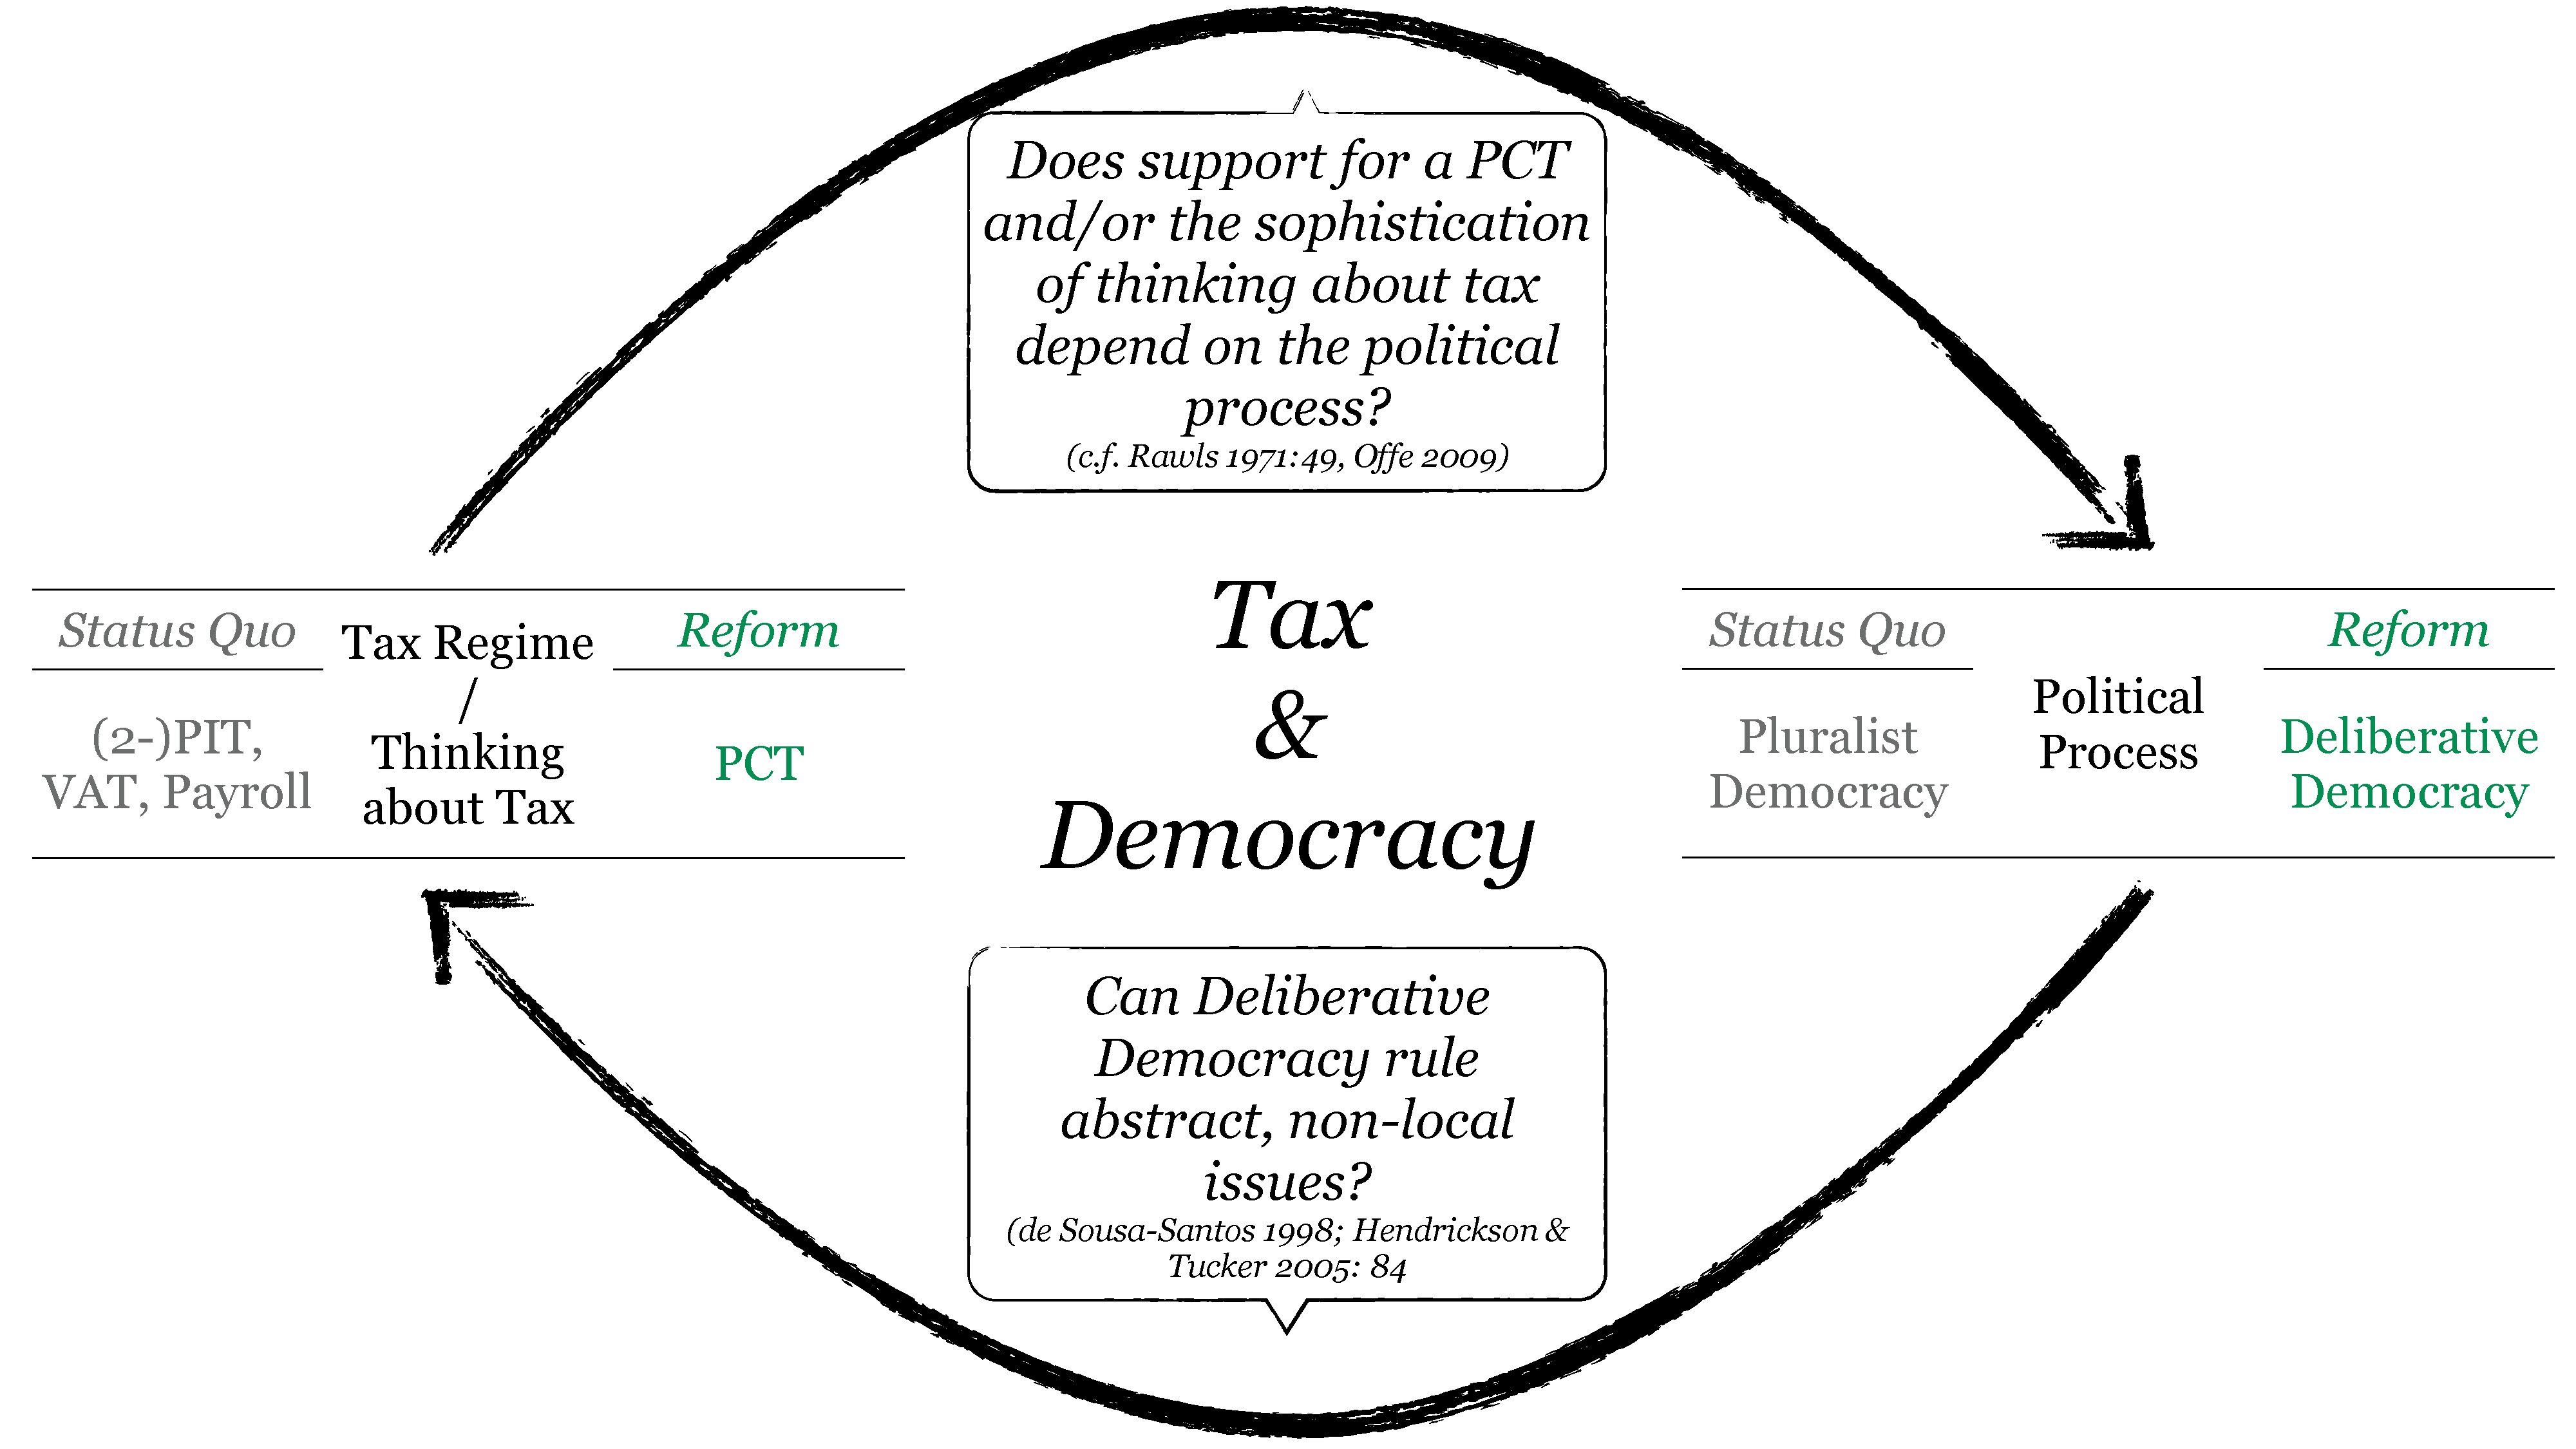
\includegraphics[width=1\linewidth]{tax-democracy}
	\caption{Taxation and Democracy}
	\label{fig:tax-democracy}
\end{figure}

Surely, such a broadly defined research agenda risks hubris, but it also promises to formulate and maybe, tentatively answer some important questions for the social sciences.
I may well --- figuratively --- be biting off more than I can chew, and it sometimes shows (for example in \autoref{chap:wanted}).
All I can do is to tentatively mull over a mouthful at a time, and spit out again that which I cannot address.
This --- forgive the metaphor --- \emph{rumination} takes a lot of pages to write and read, but at least, it is a relatively transparent way of reasoning.
Maybe, in the spirit of Umberto Eco's \emph{anti-library} \citep[as recounted in][]{Taleb2007}, explicating what I do not know or cannot address in this dissertation will make for better questions
\footnote{
	For this comparison, I am indebted to Maike Schulz, who --- citing Eco --- reminded me in 2013 that an ever elongating reading list need not be a bad thing.
}.
Still, to digest anything in full, I must concentrate.
Counterintuitively, the often economic or even technical abstractions of taxation and public choice provide a great guide here.
This mostly \emph{a priori} knowledge, too, requires a lot of pages to write and to read, but, akin to enzymes in the digestive tract, it helps me break down complex issues to ever simpler, fewer and clearer questions (as in \autoref{chap:mixed-economy} and \autoref{part:tax}) that can be handily metabolized into a new, and hopefully original argument that I put to the test.

Admittedly, too, underlying this research are normative convictions about political and economic opportunity, and even human destiny.
Somehow, such a prescriptive impetus has become unacceptable in much of (German) social science on the welfare state.
I must indeed avoid ``politics-based evidence making'' (The Economist, 2012) %add correct reference
or any other conflation of what should be, with what is.
However, even from a merely positive perspective, and even to readers who may not agree with these convictions, the hypotheticals they raise pose analytically worthy questions:
If there is indeed another, superior fiscal configuration on which we could democratically agree --- but do not --- this absence needs explaining.

If anything, finding that which needs a social explanation, must be a worthwhile attempt for the social sciences.

It, too, is how social sciences can contribute to human progress, by \emph{politicizing} the status quo.
\begin{quote}
	``Politicization is the realization that established social norms, social practices, and social relations are contingent rather than sacrosanct, that things could also be different and that citizens, individual and collectively, have political agency by means of which alternatives can be explored and implemented.
	This recognition that things could also be different has always been the igniting spark of the emancipatory-progressive movements, and politicization has always been their key strategy.''
	\\*
 	--- \citet[313]{Bluhdorn-2007-aa}
 	%add first name
\end{quote}

%If risky, this thesis has substantial analytical potential.
%This thesis illuminates the crucial, but so far underinvestigated link between democratic process and tax regime choice.
%It informs the pressing question of the sustainability of the welfare state.
%On the other hand, it tests the ability of deliberative fora to rule on matters of great complexity and large scope.
%If the experimental deliberative forum rules in favor of the PCT, it will have passed a strong test of democratic legitimacy.

%But \hyperref[sec:Wanted]{the question} can probably be answered in the negative:
%no, this is not the best of all liberal-democratic, capitalist and open worlds.

%This desirable, doable hypothetical of the perfect tax demands political science explanations:
%why are we not doing better?
% why do we settle for a structurally underfunded polity in an otherwise prosperous era?
%Why do we allow a scourge of structural unemployment to befall millions, deprived and forced into idleness?
%Why do we leave unchecked the positional excesses of our economies, in spite of the better, fairer angels of our nature?

%what's the second order theory?
%It is not an empirical question in any traditional, positivist meaning of the concept, even though it involves complex and multiple empirical assumptions and causal arguments.
%It is argued in the above, why, even from an analytical and empirical, if not entirely disinterested standpoint, said daydreaming is helpful.

%Even leaving normative considerations aside, as I have tried to demonstrate in the above, just academic rigor alone requires us to hypothesize a hypothetical of a globalized, uniformly taxed world economy.
%\subsubsection{Research Question a):
%Is it the Perfect Tax?} Research question a) is a question of normative considerations, based on which a hypothetical engineering of public policy takes place.

%\begin{description}
%	\item{\textbf{Normative Hypothetical are Needed}} Broadly speaking, it is hypothesized that, employing of a normative hypothetical in the investigation of welfare retrenchment will provide analytical added value.
%A concrete and approximately modeled alternative configuration of international tax harmonization will bring the issue into sharper focus.

%\subsection{Plan of the Thesis} Substantial groundwork is required for the bold claims I make in this thesis.
%The merits of the PCT will stand out when fundamental desiderata of taxation are thoroughly discussed.
%Conversely, the demerits of the current fiscal configuration will appear.
%To see clearly through the ``analytic muddle of tax'' (\citealt{McCaffery2005}:
%862) I have to zoom out, establish some abstractions, dynamics and norms of welfare, allocation and inequality seemingly remote to any worldly tax reform.
%They are not.

	%here's the beauty.
%I get to do an empirical work.
%I make this FALSIFIABLE.

%What's the result?
%What happens then?
% pluralism
%delta in attitudes, knowledge etc.
%theory building, critical analysis
%Deliberative Democracy:
%is interest out?
%(yes!)

%Generally, note the Rawlsian, or theory-driven case selection (saturation sampling) backup to representativenss.
%It's not about aggregation.

%4) Can the PCT be implemented nationally?
%That is important for the Deliberative Poll.

%Remember, however, that you don't need perfect absence of prejudice or inequality or ideal speech.
%You just need spech that's a little better than pluralist speech, and a little better than markets.
%Just like Caplan's argument.(this also in response to sanders)

% * step back carefully from my assumptions:
%even if you don't agree with the politics (redistributive and axiomatic in terms of positional spending) of the pct, you've gotta agree with the efficiency.
 %  * even if you don't agree with the PCT, you've gotta agree with the questions it poses.

%Ich hoffe so dem pluralistischen Steuerdiskurs einen (jedenfalls näherungsweise Habermas'schen) Diskurs gegenüber stellen zu können.
%Sollten sich, wie ich annehme, zwischen diesen beiden qualitativen Daten systematische Unterschiede im (Miss)verständnis von Steuer heraus stellen, könnte ich erste Hypothesen über den Zusammenhang von politischem Prozess/Ideal (pluralistisch vs.\ deliberativ/Habermas) und polit-ökonomischem Diskurs ableiten

%I want to (qualitatively) compare the thinking about tax in two very different samples:
%a) expert interviews (politicians, lobbyists) and b) a deliberative jury of randomly selected citizens (Cohen, cf.~Habermas).
%My data will be the discussions in these two samples.
%I assume these samples to reflect two paradigmatic (most different) democratic fora or processes, onepluralist (experts aka.
%interest group reps) one deliberative (jury members).
%My "hypothesis" (I know I'm not supposed to have a hypothesis, this will be an inductive/qualitative endeavour) is that these two democratic fora will differ systematically in the kind of thinking about tax and redistribution that they produce.

%.
%My 2nd order theory of tax is democracy.
%My 2nd order theory of democracy is inequality.
%Offe says:
%write a Konflikttheorie, a 2nd order theory on the reform suggestion (such as Offe 2009)

%Explain how the empirical, testable approach would look.
%But point out:
%there needs to be a plan B, paddle back from this.
%For normative (Cervantes) reasons but also because these are stupid shorthand understandings.

	%overview of what is to come;
%next chapters
%And what kind of research design is this?
%(it's an extreme case)

%\section{Schedule}

	%There is a vibrant and innovative community of scholars and activists who host and moderate deliberative fora of varying designs, particularly in the US.
%Organizing successful deliberations is at least as much an art as a science and requires extensive experience.
%In addition, I must prevent my analytical and normative preoccupation with a particular reform proposal (a postpaid PCT) from exerting undue influence on the deliberation.
%The deliberative must not be set up to confirm the PCT.
%Both hypothesis a) and b) must be falsifiable in this design.
%A postpaid PCT must be presented as one of the (few) fundamental choices in redistributive design.
	%My prior work (Held 2010) on the postpaid PCT can serve as a survey of the trade-offs and desiderata (see summary above) in redistributive design.
%These may serve to organize the expected transformation of previously “amalgamated” (Miller 1992:
%4ff) preferences into distinct, single-peaked dimensions.
% The trade-offs and desiderata are also inputs for questionnaire design and may be used to draft briefing materials.
	%This quasi-experimental design requires great methodological care and experience.
% Ideally,  I will be able to co-host, or investigate a Deliberative Poll ® on redistributive design in Germany or the US, with help from James S.
%Fishkin and the Stanford-based Center for Deliberative Democracy.
% This would ensure rigorous institutional design, peer-reviewed balance and experienced implementation, but requires substantial external (to BIGSSS) funding.
%Should I be unable to secure such funding, some scaled-down version will also be possible.


%%%
\section{Operationalization}

%\cite{Johnson1998}
	%161:
%``Would-be political reformers of various persuasions urge deliberation upon us.
%Yet in their pleadings such theorists and reformers frequently invoke deliberation in an uncritical manner.
%They proceed as though the ways in which deliberation and the effects we can expect of it are not just obvious, but attractively so.''

%\cite{Azmanova2010} (also \cite{Fishkin2009}:
%529)
	%49:
%thoughtfulness and reflexivity (as per Fishkin) require 1) reasonably accurate information 2) substantive balance 3) diversity, 4) conscientiousness, 5) equal consideration

%\cite{Citizen-2004-aa}
	%11:
%one guy did the learning sessions
	%1) has a selection phase
	%2)  has a LEARNING phase
		%also develop "shared values" about the process
	%3) has a PUBLIC HEARING phase
	%4) has a DELIBERATION phase
	%go to church with group, maybe.

%\cite{Dienel-1999-aa}
	%"To make a Planning Cell project go effectively, one needs a process of more than four days.
%We can distinguish five phases:
%design, preparation, implementation, compiling the documentation, follow up.
%After the joint formulation of the task, two problems have to be solved in the second phase:
%The issue has to be translated into a program of 16 work units and the jurors have to be selected and invited.
%Building the program is crucial for the Planning Cell preparation.
%Each working unit has to have its clearly defined remit.
%Problems have to be reduced to comprehensible alternatives.
%All this is done by the programmer who is much more important than the moderator''

%\cite{Fung-2003-ac}
	%very good summary, get back to this

%\cite{Fishkin2009}
	%democracies are supposed to fulfill two values;
%political equality and deliberation (loc.~84)
	%``a democracy in which we all had substantive information [and] [\ldots] substantive opinions would seem to take too many meetings.''
	%what's wrong with unenlightened opinions (all loc.~113ff)
		%\begin{enumerate}
			%\item they may be volatile (cite other sources
			%\item people may be manipulated by foregrounding some information (clean coal vs.\ dirty coal, forgetting about natural gas -- compare this to tax choice)
			%\item misinformation (savings rate)
			%\item favor favorable, true arguments over others
			%\item manipulation may ``prime'' one aspect of policy.
		%\end{enumerate}
	%loc.~260:
%``the hard choice, in other words, is between debilitated but actual opinion, on the one hand, and deliberative but counterfactual opinion, on the other.''
	%loc.~369:
%table with raw/refined opinion, and different kinds of sampling.
	%loc.~438:
%``The idea is that if a counterfactual situation is morally relevant, why not do a serious social science experiment -- rather than merely engage in informal inference or armchair empiricism -- to determine what the appropriate counterfactual situation might look like?
%and if that counterfactual is both discoverable and normatively relevent, why not then let the rest of the world know about it?
%Just as John Rawls's original position can be thought of having a kind of recommending force, the counterfactual representation of public opinion identified by the Deliberative Poll also recommends to the rest of the population some conclusions that they ought to take seriously.''
	%loc.~390:
%self-selected samples will be very limited in what they can achieve.
	%loc.~401:
%citizen juries use quota samples, consesus conferences use self-selected samples, then with some quota sampling
	%loc.~550:
%notes that positions must not merely be balanced in terms of airtime or affect, but ``whether the considerations offered in favor of, or against, a proposal, candidate or policy are answered in a substantive way by those who advocate a different position.''
	%loc.~561:
%three categories for such considerations
		%``the benefits or burdens of a policy or political choice,
		% the causal arguments about whether those benefits or benefits or burdens will actually result from one choice or another,
		%and the values by which those benefits and burdens might best be evaluated.''
		%loc.~1424:
%``the problem is that any microcosmis deliberation taking place in a modern society will be one in which there are significant social and economic inequalities in the conduct of ordinary life in the broader society.
		 	%It seems difficult or impossible to `bracket' these inequalities -- for participants to behave `as if' they do not exist.
		 	%Indeed the problem goes deeper.
%The possibility of doing so is the challenge of the ``autonomy of the political'', namely, whether or not equality can hold sway in politics in a world in which inequality rules in economic and social relations.
		 	%The viability and legitimacy of the liberal-democratic process may turn on the answer.''
		 	%notes that the relation between ideal theory and actual practice is ``aspirational'' \citep[loc.~2679]{Fishkin2009}


%\cite{GutmannThompson-2004-aa}
	%loc177:
%`your fellow citizens must give reasons that are comprehensible to you''
	%loc.~188:
%they introduce first and second-order theories, too!
	%loc.~919, writing about Fish:
%``Giving reasons is the chief way of academics to exercise power in democratic politics.
%All the talk about deliberation, like deliberation itself, is merely a cover for power politics.''.

%cite the sausgruber tyran stuff.

%iris marion young, especially notes that people of lower status may have a hard time getting listened to, or that others may be particularly accustomed to orderly forms of reason-giving arguments that weigh with other participants -- and this may be particulary problematic the more substantive the topic is.

%note that

%groupthink!

%tax allows only very limited choice:
%income, consumption or assets;
%a couple of schedules, plus some pigouvian taxation.
% the CIT, notably, is just a special way to raise the PIT.
%Otherwise, only natural persons.
%Tax demands these choices.
%Also, these choices \emph{are} as I explain in the below, political, so they must be made legitimately, and we may not be able to simply outsource them to elites.

%argue exactly why small sub-issues of tax do not work;
%they violate the real choices.

%there remain problems:
%you can't just go about this as if it wwere not controversial;
%it is controversially maongst experts, but more importantly, controversial whether experts have in fact authority and the right context.
%It can't just be an experiment, or a treatment intervention where ordinary citizens must necessarily become more like experts, and if they are not, then the teaching has failed.
%It must be possible for people to disagree with the abstractions they ar epresented with, see the criticism of it.

%tax is very technocratic, simply because the instition is like that.
%this will have to be qualitative


%\end{enumerate}


\part[The Crime Scene of Tax]{The Crime Scene of Tax:\ First Order Theory}
	\label{part:tax}
	\chapter[Desirable Tax]{A Desirable Tax}
		\label{chap:desirable-tax}
		%!TEX root=../tax-democracy-held.tex

\chapter[Desirable Tax]{A Desirable Tax}\label{chap:desirable-tax}

%quote needed

%here, now, comes the first-order normative criteria: what would make it nice?

% What makes a more efficient, more equitable tax?
% This concerns the conceptual and normative building blocks of taxation. Sufficient analytical clarification on a “new understanding of tax”, with particular regard to the PCT has been reached (McCaffery 2002).

%add on "property" Simons' argument that it's 90 percent background conditions, and Offes (2009 via Bosch) addition that rents of cooperation (cf game theory) can, by definition, not be accrued to any one PARTICULAR participant.

To design and choose a normatively superior tax, we need criteria against which to measure alternative regimes. A normatively superior tax will satisfy and balance \hyperref[sec:Efficiency]{efficiency} (page \pageref{sec:Efficiency}) and \hyperref[sec:Equity]{equity} (page \pageref{sec:Equity}) norms. It will also be \hyperref[sec:sustainability]{sustainable} (page \pageref{sec:Sustainability}) over time. %this needs to be re-written, the below sections have changed

\section[Optimality]{Optimality: Desirable Taxes Are Neutral \textsuperscript{\ref{fn:also-in-mpp}}} \label{sec:tax-optimality} %this used to be called efficiency, but I changed the heading.
A system is efficient if it maximizes outputs for given inputs.

%somewhere in McCaffery: Ramsey optimal tax literatre: "inverse elasticity" rule. This can lead to perverse ideas: working wifes is ok, but low wages for immigrants with hig hwork ethic?

\paragraph{Which Efficiency Norm?}
But exactly \emph{what} should be maximized? Efficiency norms vary and can conflict. I present here three popular definitions in increasing order of strength\footnote{
	The selected efficiency principles are all cardinal, rather than ordinal in definition, and do all not consider the aggregation problem commonly known as \emph{diminishing utility to wealth} \citep{Hicks1946}. While these are substantial shortcomings, they do not concern me in the efficiency discussion of the perfect tax. Respective \emph{equity} implications are discussed in sections \ref{sec:DiminishingUtility} (\hyperref[sec:DiminishingUtility]{diminishing returns}) and \ref{sec:ConspicuousConsumption} (\hyperref[sec:ConspicuousConsumption]{conspicuous consumption}).}.
Earlier entries are subsets of later entries, as visualized in \autoref{fig:Efficiencies}.

\begin{description}
	\item[Pareto Efficiency.] \phantomsection \label{sec:Pareto} An allocation is pareto-optimal, when no one can be made better off \emph{without making someone else worse off}. Pareto optimality, is, in fact not a pure efficiency norm but includes an equity component, too.
	\item[Kaldor-Hicks Efficiency.] \phantomsection \label{sec:KaldorHicks} An allocation is Kaldor-Hicks efficient, when no one can be made better off without making someone else worse off \emph{by the same or a greater amount} of disutility \citep{Kaldor1939,Hicks1939}. It can also be described as a pareto-optimal outcome where sufficient compensatory sidepayments can be made from the winners to the loosers.
	\item[Social Welfare Optimum.] \phantomsection \label{sec:swo} The pure efficiency norm is given by the utilitarian slogan ``The greatest good for the greatest many'' \citep{Mill1863}. It knows no equity at all, but is concerned only with the sum total. It is also known as a social welfare optimum in game theory (for example, \citealt{Oye-1985-aa}).
\end{description}

\begin{figure}[htbp]
	\centering
	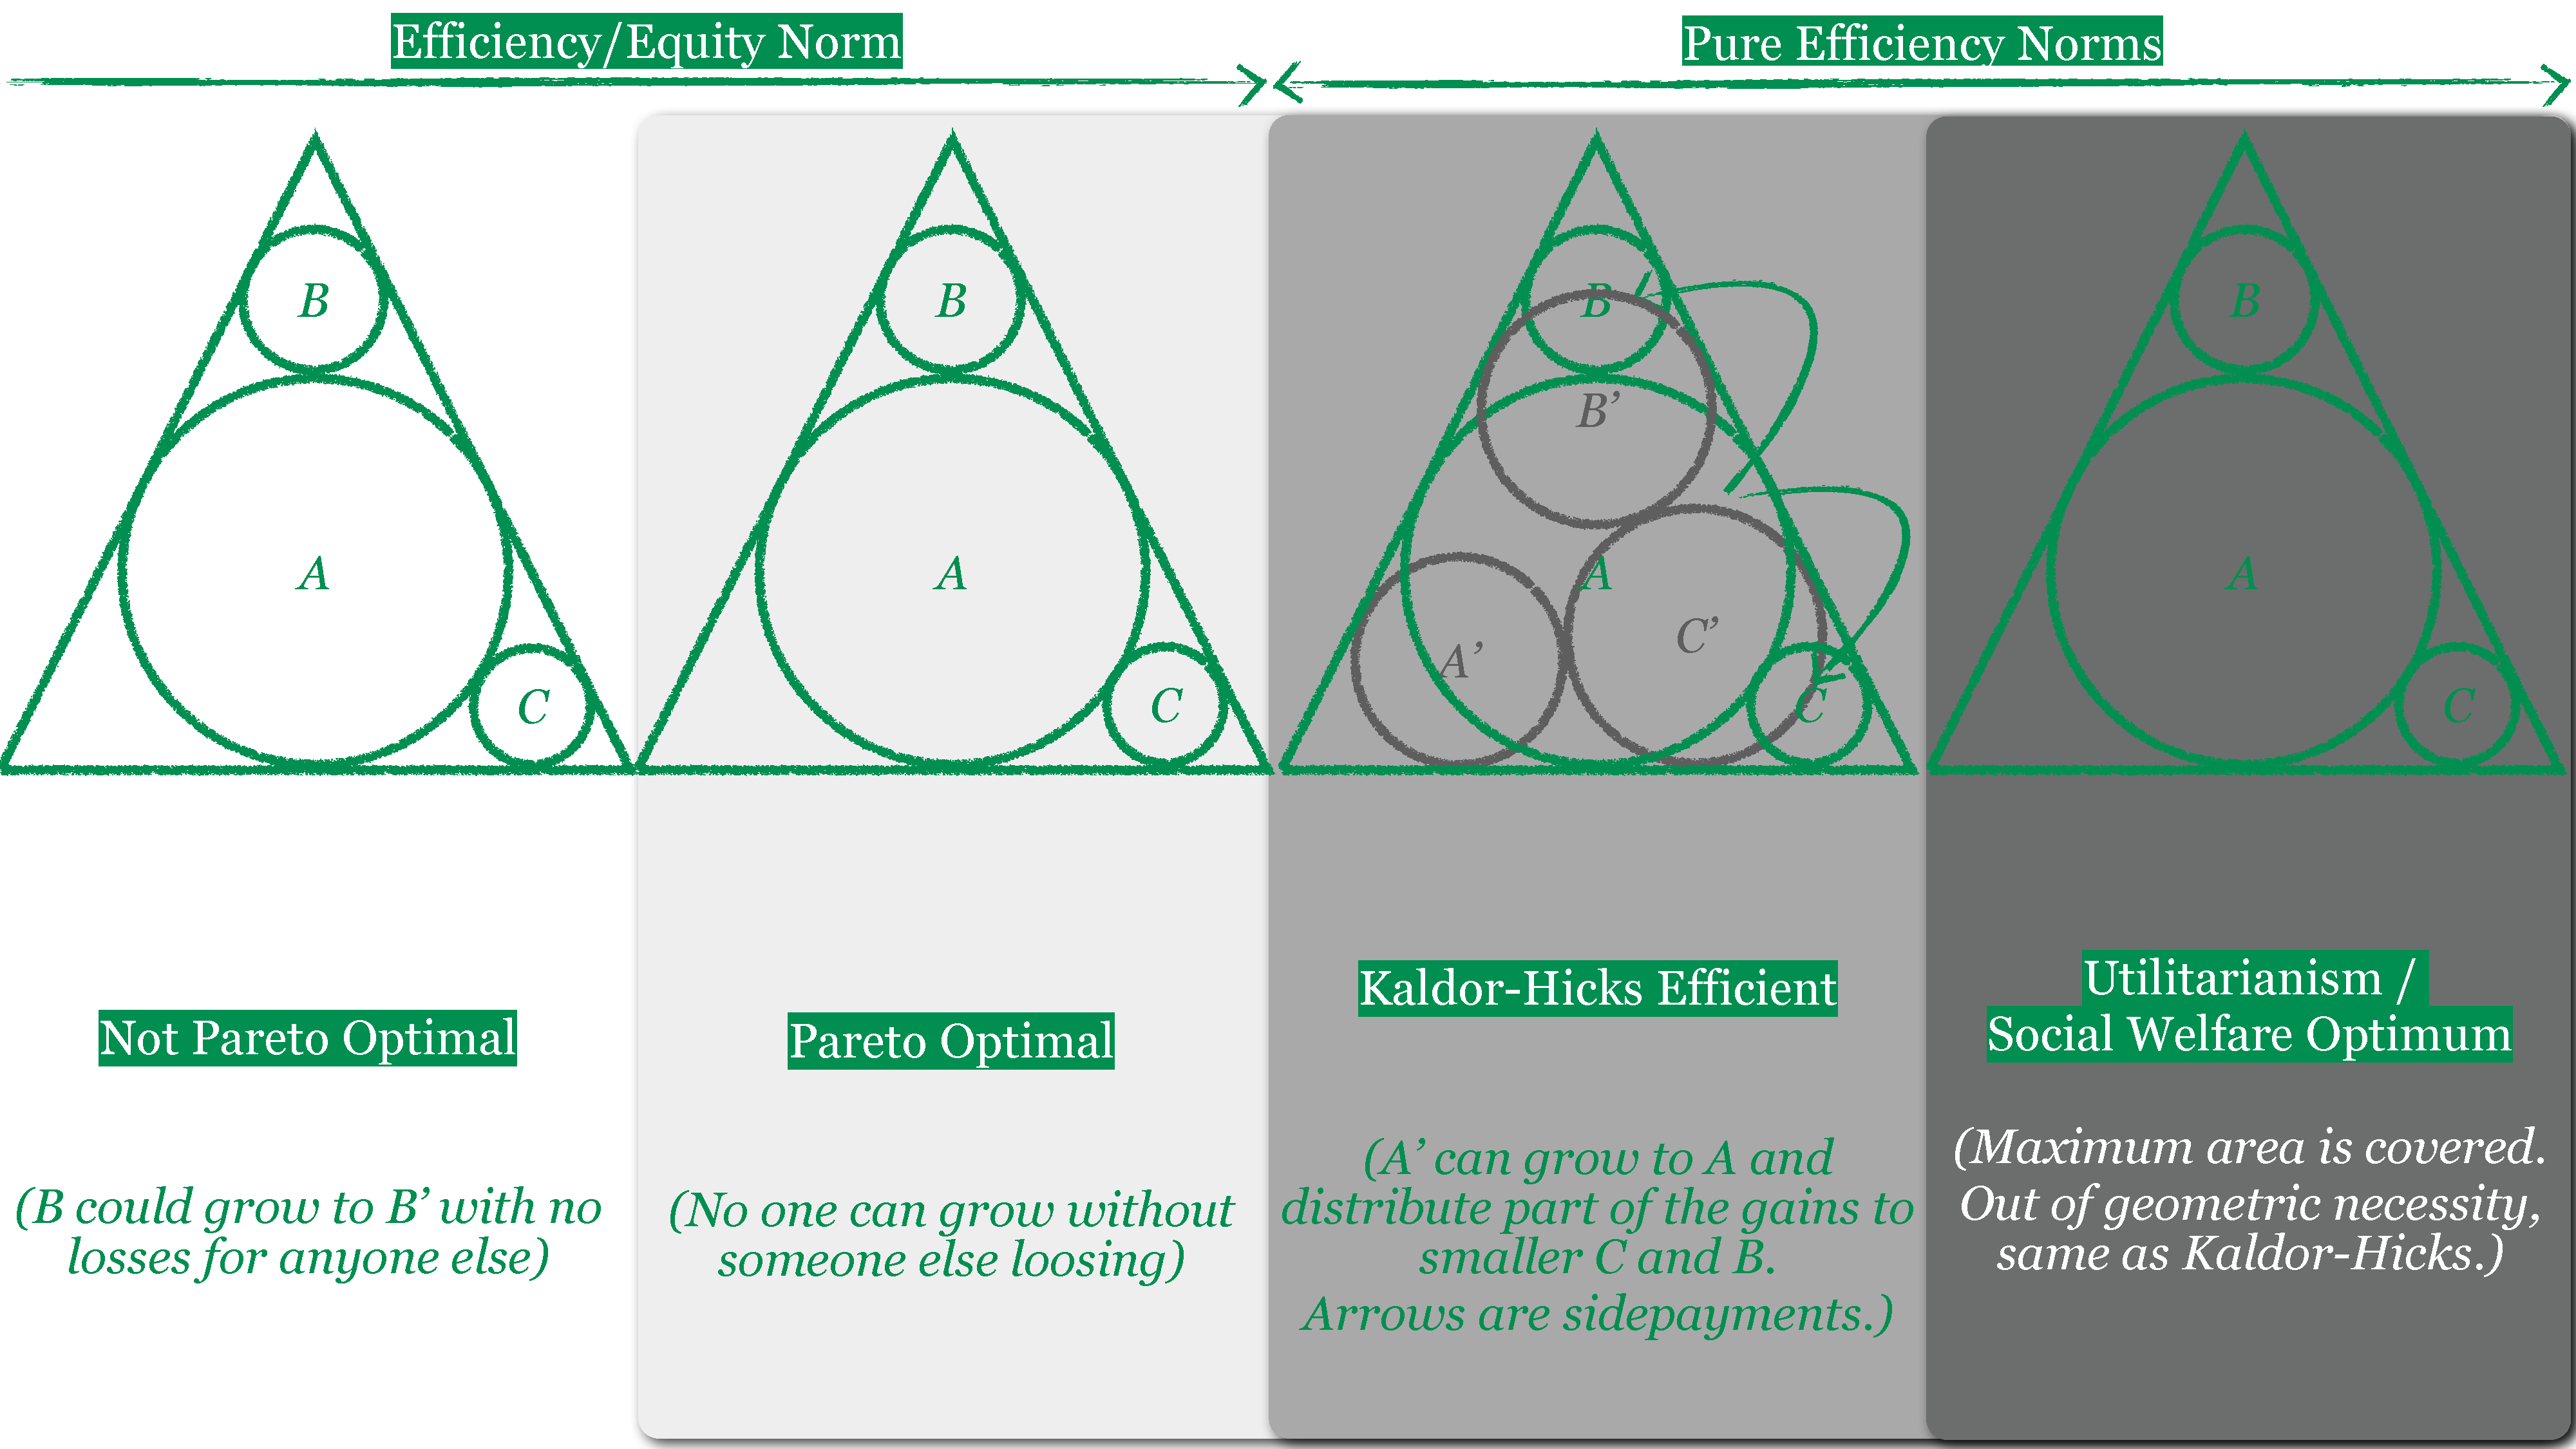
\includegraphics[width=1\textwidth]{efficiency-norms}
	\caption[Selected Efficiency Norms]{Selected Efficiency Norms, Where Area Equals Utility}
	\label{fig:Efficiencies}
\end{figure}

I choose \hyperref[sec:Pareto]{Pareto optimality} as the weakest of these efficiency norms and note whenever a stronger efficiency norm is required for an argument. Pareto efficiency is also widespread efficiency norm that is convenient for its link to \hyperref[sec:PerfectCompetition]{perfect competition} (page \pageref{sec:PerfectCompetition}).

\paragraph{In Dubio Pro Mercatus.}
The above posited perfect markets can be shown to work Adam \citeauthor{Smith-1776-lq}'s \emph{Invisible Hand} \citeyearpar{Smith-1776-lq}. More formally, the first theorem of welfare economics states that any competitive equilibrium will be Pareto optimal: no one could be made better off, without making someone else worse off\footnote{Demonstrated first graphically by \cite{Lerner1944}, mathematically by \cite{Lange1934}, \cite{Debreu1954} and others.}.

For (\hyperref[sec:Pareto]{Pareto}) efficiency, the burden of proof then lies on state interventions in \hyperref[sec:CompetitiveMarkets]{competitive markets}. It follows that a tax should affect market interactions as little as possible.

\paragraph{Minimize Deadweight Losses}
The efficiency loss that \emph{does} occur when taxes alter market interactions is called a deadweight loss (DWL), illustrated in \autoref{fig:DWL}. It arises as follows: consumers and producers both reduce their buying and selling, as consumers face higher and producers lower prices. This reduces the welfare, or surplus of consumers and producers. Some of this loss is transferred to government. The net that is not recouped as tax revenue is the deadweight-loss of taxation. %note, improve language-wise: DWL is the opposite of gains from trade.

%the question is: why is the DWL here, and not in some other section, namely do ability?
%this figure happens earlier as fig:DWL

\begin{desideratum}[Minimal Deadweight Loss]
	A desirable tax should have a minimal deadweight loss.
	\label{des:DWL}
\end{desideratum}

\begin{desideratum}[Incentives]%is this not the same as DWL?
	A desirable tax will maintain and strengthen incentives to maximize private, unobserved effort in work and investment.
	\label{des:Incentives}
\end{desideratum}

%note somewhere that this applies only to revenue generation and redistributive taxation; pigouvian is the opposite

\subparagraph{Reformulations of DWL.} The idea of the DWL of taxation can be reformulated in a number of ways\footnote{The DWL of taxation is later derived from the \hyperref[sec:TaxInelastic]{price elasticities} (page \pageref{sec:TaxInelastic}) of supply and demand.}.
\begin{description}
	\item[Factor Unemployment] refers to DWLs in markets of factors of production, when tax wedges cause incomplete employment of labor or capital. This problem is particularly dire in the indivisible supply of low-productivity labor, where entire strata of workers may be unable to find gainful employment at post-tax wages. This problem of \hyperref[sec:StructuralUnemployment]{\emph{structural} unemployment} is further discussed in \autoref{sec:InequalityIsInefficient} and addressed in desideratum \ref{des:LowPriceFloor}.
	\item[Taxes are Anti-Growth.] A sophisticated version of this sentiment will also argue that widespread DWLs waste economic resources in the medium and long run.
	\item[Neutrality.] The DWL of a tax can also be described as its impact on a hypothetical, before-tax, pareto optimal market. An efficient, desirable tax is neutral in the sense of leaving pre-tax relative prices unchanged (\citealt{McCaffery2005}: 849).
\end{description}

%\paragraph{Savings Must be Earned.} The discussion of savings here, as elsewhere, concentrates on the trade-off between \emph{saving} and \emph{consuming}. However, before money can be either saved or consumed, it has to be earned. Another trade-off between \emph{leisure} and \emph{work} applies here. Just like saving (desideratum \ref{des:Savings}), this trade-off also has to be adequately incentivized \citep{Frankel1998}. In addition to desideratum \ref{des:Savings}:

%introduce work-leisure as a sub-class of DWL or rather, neutrality.
%\begin{desideratum}[Arbitrary Work-Leisure Incentive]
	%A desirable tax should allow for arbitrary, negative incentives for the consumption of leisure.
%	\label{des:leisure}
%\end{desideratum}

%same thing applies to spending and saving
	%is also a sub-class of the DWL
	%consider discussing the OSN and Y2C here, they are sort of exceptions to this rule
	%note that this also has fairness implications that cut both ways.

%maybe the whole issue of capital/agnosticity also belongs in here, maybe this is really just a sub-class of DWL.

%here used to be a section on welfare gains from taxation, but that is now over at mixed economy.

%in here was the section on different kinds of fiscal interventions. It has now moved to "mixed economy".

\section[Justice]{Justice: Desirable Taxes Are Fair} \label{sec:tax-justice} %this used to be called equity, but that is now in mixed economy
I assume here, axiomatically, that some degree of post-market  equity is desirable. %further introduction is neeeded

%here, I still have to write a bit on distributive justice
	%http://en.wikipedia.org/wiki/Justice#Theories-of-distributive-justice
	%http://en.wikipedia.org/wiki/Distributive-justice
	%compare them, explain why I go for Rawls

%In philosophy, the term "maximin" is often used in the context of John Rawls's A Theory of Justice, where he refers to it (Rawls (1971, p. 152)) in the context of The Difference Principle. Rawls defined this principle as the rule which states that social and economic inequalities should be arranged so that "they are to be of the greatest benefit to the least-advantaged members of society". In other words, an unequal distribution can be just when it maximizes the mininum benefit to those who have the lowest allocation of welfare-conferring resources (which he refers to as "primary goods").[5][6]
	%note that this is only loosely related to the maximin use otherwise used.

%\subsection{Natural Persons}

%The first complication of taxation is actually a clarification: redistribution is only meaningfully defined between \emph{natural} persons, that is, actual human beings. William \citeauthor{Vickrey1947} begins his classic \emph{Agenda for Progressive Taxation}: ``Genuinely progressive taxation is necessarily personal taxation'' (\citeyear{Vickrey1947}: 1).

%comment here somehow on the foundational argument: that you are entitled to whatever you earn in uncoerced exchange --- or are you?

%also comment here somehow on where that relies on the state
	%in protection of property rights for private consumption
	%in protection of land etc. for control
	%na this isn't so good.

%we know from earlier desiderata, we want it to be progressive, but just how and why we want that is less clear. that's why this is about fairness, not just equity.

\subsection[Foundational Arguments]{Foundational Arguments}
%somehow set them up here? that stuff that has been earned through uncooerced exchange ...
%set myself up for the later foundational arguments on the PCT and the LVT.

\subsection[Distributional Justice (as Fairness)]{Distributional Justice as Fairness: When is Inequality Unjust?}
%here, I moved two paragraphs of rawls to wanted. Transition missing.
\paragraph{Distributional Justice.} Second, Rawls suggests two distributive norms, the \emph{difference principle} and the \emph{fair equality of opportunity} \footnote{
	These two distributive norms follow the equal liberty principle in \emph{lexical} order, meaning that no distributive improvements can justify infringements of equal liberties.}.
Under the \emph{difference principle}, differences in endowments as well as subsequent social and economic inequalities are acceptable only if their granting also benefits the least fortunate\footnote{
	\citeauthor{Rawls-1971} (\citeyear{Rawls-1971}: 122) warns that this calculus must not only include strictly economic payoffs, but must also take into account the intangible correlates of social inequality as societal and cultural participation, as well as confidence.}.
If inequities cannot be thereby justified, such undeserved differences (by birth or other random allocations) in endowment should be corrected by intervention for \emph{fair equality of opportunity}.

This latter norm of fair equality of opportunity is a pure equity norm on the equality of inputs.

The difference principle is more complicated. It combines equity and efficiency norms. It is that weak pareto optimum (WPO)\footnote{
	An allocation is weakly pareto optimal when no other allocation is \emph{strictly} preferred by everyone. A strong pareto optimum, by contrast, requires only that all individuals will receive same \emph{or} higher payoffs.},
which maximizes the minimum payoff (maximin) in outcomes. \autoref{fig:distributive-norms} illustrates the two Rawlsian norms of distributive justice in context. %easy to understand formulation required

\begin{figure}[htbp]
	\centering
	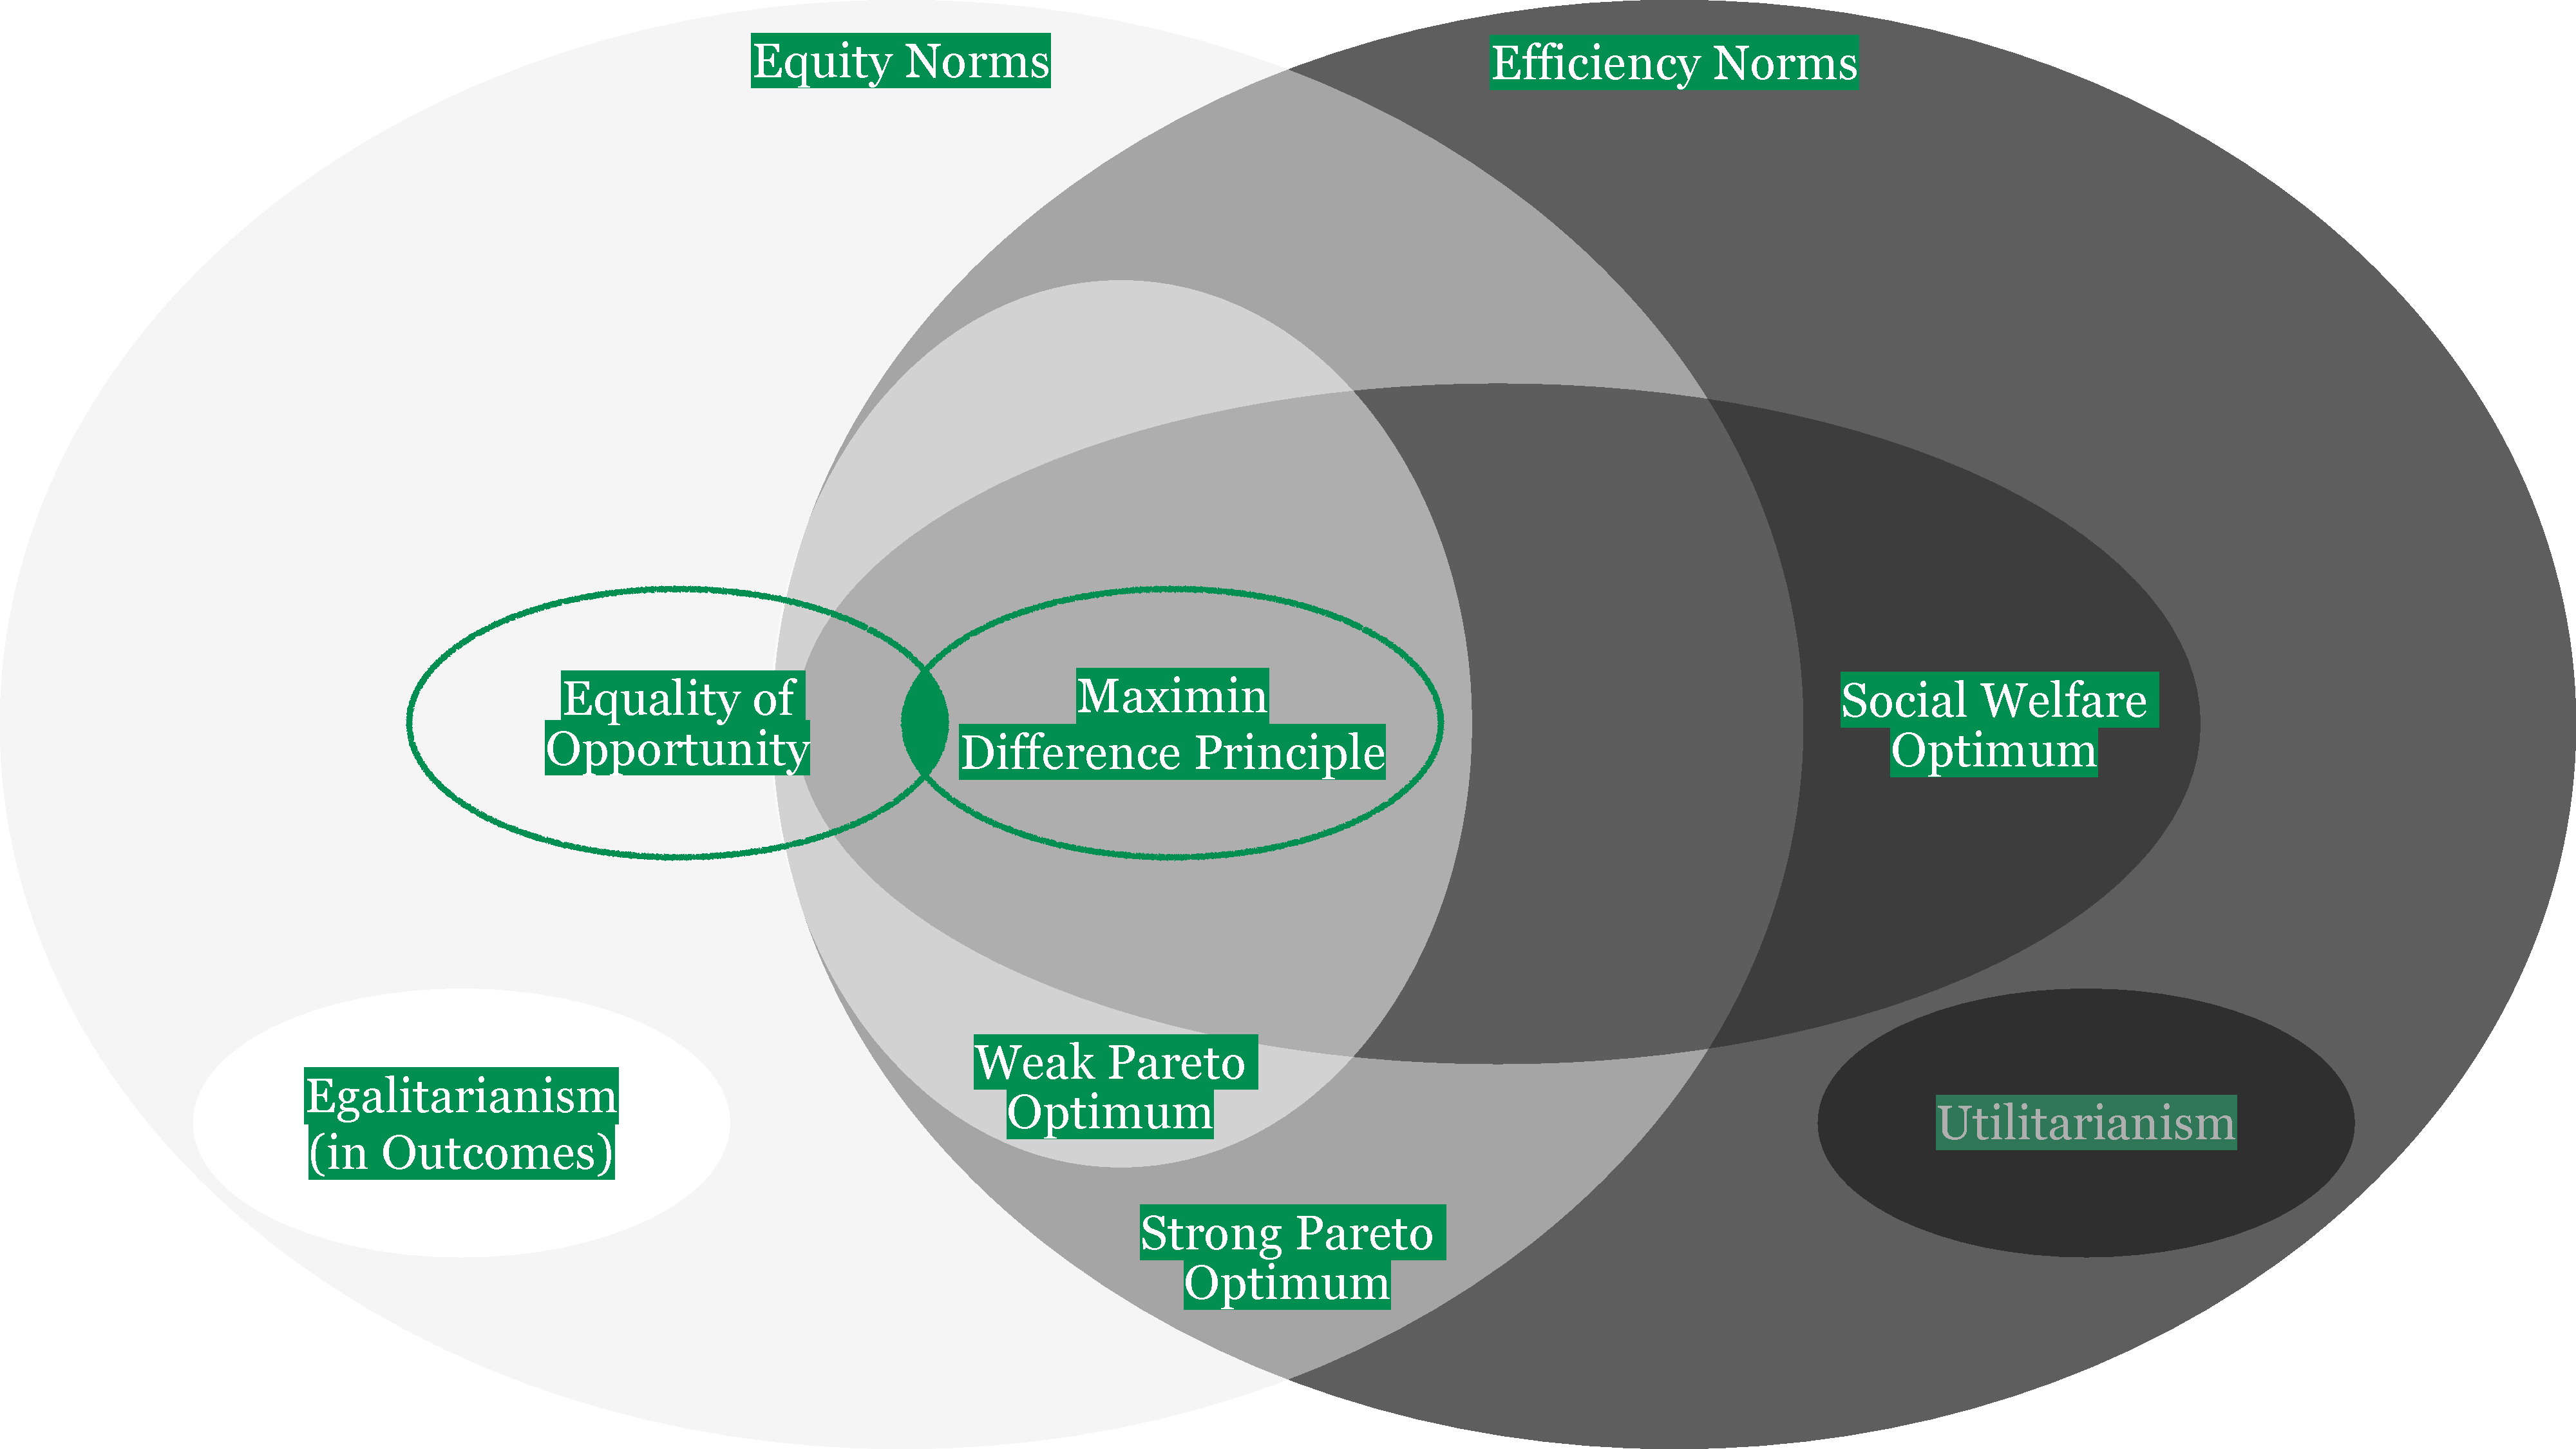
\includegraphics[width=1\textwidth]{distributive-norms}
	\caption[Selected Distributive Norms]{Selected Distributive Norms and Rawlsian Distributive Justice (in green)}
	\label{fig:distributive-norms}
\end{figure}

\paragraph{Why Rawls?}
Any comprehensive discussion of distributional justice is beyond the scope of this thesis. \citeauthor{Rawls-1971} \emph{Theory of Justice} is presented here for four reasons.

First, \emph{justice as fairness} serves as a convenient cut-off point on a (crudely) imagined continuum of theories of distributive justice from left to right, from egalitarianism to utilitarianism and liberitarianism\footnote{A right-hand pole comprising of utilitarian \emph{and} libertarian ideals obviously reveals the futility of any one-dimensional scaling of theories of allocative justice.}. It is assumed that all allocative norms ``left of'' Rawls (c.f. \citealt{Cohen2000}), stressing equity over efficiency will strictly prefer the PCT over the status quo. Conversely, theorists on the right end of the imagined continuum (for instance, \citealt{Nozick1974}) may not share all of the normative foundations of the PCT, or even prefer it over the status quo.

Second, the \emph{difference principle} is \hyperref[sec:FoundationalBeauty]{invoked} (page \pageref{sec:FoundationalBeauty}) when I argue the normative superiority of the progressive taxation of consumption.

Thirdly, in arguing that the PCT is the perfect tax, I attempt to establish it as an \emph{reflective equilibrium} (\citealt{Rawls-1971}: 49) emerging from a pragmatic-spirited back-and-forth between what is \hyperref[sec:desirability]{desirable}, and what is \hyperref[sec:feasibility]{doable} (\citealt{McCaffery2005}: 856).

Fourth, \citeauthor{Rawls-1971}' \emph{Theory of Justice} (\citeyear{Rawls-1971}) is an end-state theory of distributive justice (\citealt{Fried1999}: 1007), not a procedural prescription (for example \citealt{Dahl-1989-aa}). This thesis, likewise, hypothesizes a normatively superior allocative outcome (``Is this the best of all \ldots'', c.f. page \pageref{sec:Wanted}). A political process, aside from \citeauthor{Rawls-1971}ian liberty, is not prescribed in its own right. It merely serves as an \emph{independent} variable in \autoref{sec:WhyNot}, explaining and criticizing why it may have failed to deliver the superior allocative outcome.
	%elaborate this further, Kohler's comment ``your're an economist'', ideas as explanandum may apply here

\paragraph{Implications for Tax Design.}
Two desiderata for tax design emerge from \citeauthor{Rawls-1971}'s Theory of Justice.

First, the principle of \emph{fair equality of opportunity} introduces equity as a goal for taxation. It is a general and unspecific norm. Translating it into a desideratum for tax design hinges on an empirical assessment of  opportunity
	%
 in the real world. A specification of this norm must therefore await an inspection of the \hyperref[sec:GovDynofIneq]{governing dynamics of inequality} (page \pageref{sec:GovDynofIneq}) in modern society. It is provided in desideratum \ref{des:SharpProgression}.

Second, the \emph{difference principle} provides a more straightforward guideline for redistributive taxation. It implies that taxation should exempt from redistribution economic inequality if, and to the extent that, it makes the least fortunate better off. This may occur when able people require economic \hyperref[des:Incentives]{incentives} to exert maximum efforts (desideratum \ref{des:Incentives}), or when \hyperref[des:Entrepreneurship]{smart investors}, acting in their own self-interest, can be trusted to make good production decisions (desideratum \ref{des:Entrepreneurship}). Because axiomatically assumed perfectly competitive markets can be shown to be pareto optimal, it follows that:

\begin{desideratum}[Difference Principle]
	A desirable tax exempts from redistribution economic inequality if, and to the extent that, it makes the least fortunate better off.
	\label{des:DifferencePrinciple}
\end{desideratum}

Generally, for axiomatically assumed \emph{homo economicus} to \hyperref[sec:PerfectCompetition]{perfectly compete}, she needs incentives. Desideratum \ref{des:Incentives} is closely related to desideratum \ref{des:DWL} (\hyperref[des:DWL]{minimal DWLs}).

%discuss somewhere: vertical vs. horizontal equity (\citealt{Mankiw-2004-aa}: 255); this is key for a rule-of-law, fair tax. It's also the same norm as gleiches wird gleich, unterschiedlich unterschiedlich behandelt, somewhere in the German Basic Law. Find out where.

\section[Sustainability]{Sustainability: A Desirable Tax Ensures Future Prosperity} \label{sec:tax-sustainability}%definietely need better title

%think about making this into a catch-all thing: capture here both the time-inconsistency stuff as well as the commons failures et al.

%also need a standard here, maybe the solow growth stuff? not sure. or maybe, the standard is simply to have an arbitrary savings rate set by the democratic sovereign? no ... it must be at least Solow, clearly.

Social and economic systems are dynamic systems: they evolve over time. Their change is predominantly \emph{anthropogenic} or \emph{endogenous}, with the exception of very sparse or very slow variations in natural systems. Tomorrow's economic output will, to the largest extent, be a function of today's economic
	%really?
configuration --- except, of course, if another extinction event hits or another ice age\footnote{
	Then again, the jury is still out on whether another anthropogenic ice age is in the making \citep{UnitedNations2007, Rahmsdorf-2009}.}
sets in \citep{Courtillot2002}.

It follows that a desirable fiscal allocation should also contribute to sustainability. I exclude here narrower defined environmental and social dimensions of sustainability and relegate these \hyperref[CommonGIcood]{Common Goods} to be internalized through Pigouvian taxation. Instead, I concentrate on pure fiscal sustainability over time, or \emph{intertemporal optimization} in the \hyperref[ShortTermSmoothing]{short-} and \hyperref[LongTermSmoothing]{long-}term.

Sustainability bears both on equity and efficiency. An equitable policy ensures same (discounted) utility for people living today vs. people living in the future. An efficient policy ensures maximum (discounted) growth over all periods. As both criteria often overlap in concrete policy issues, they are discussed together here.

How can taxation help us prosper tomorrow and in a generation? The answer depends on the chosen time horizon.

%\paragraph{Both Equity and Efficiency Apply.} Policy recommendations for intergenerational allocation bear equally on equity \emph{and} efficiency. Sustainability is a goal of
%\hyperref[sec:IntertemporalEquity]{\emph{intertemporal equity}}: under a pure equity norm, future generations should enjoy the same prosperity as the current generation (this implies zero growth). Conversely, growth is a goal of \hyperref[sec:IntertemporalEfficiency]{\emph{intertemporal efficiency}}: under a pure, \hyperref[sec:swo]{utilitarian} efficiency norm (page \pageref{sec:swo}), the world economy should expand as fast as exogenously possible (irrespective of generational incidence).

%%%%%%%%%%here comes more stuff from a random document: https://docs.google.com/document/d/1uFpQLhFxSPVstd3WjEr_HkFXj_uyANlmvKtBxC3LGC0/edit
	\chapter[Doable Tax]{A Doable Tax}
		\label{chap:doable-tax}
		%!TEX root=../tax-democracy-held.tex

\chapter[Doable Tax]{A Doable Tax}\label{chap:doable-tax}

%add comment, footnote: this was first submitted as ...

%``analytic muddle of tax'' (\citealt{McCaffery2005}: 862) 

\begin{quote}
	\emph{Things in tax are bad today.}\\*%better quote
	--- Edward J. \citeauthor{McCaffery2005} (\citeyear{McCaffery2005}: 893)
\end{quote}

%McCaffery:
	%There are four particularly important ones in tax: the taxable unit, the tax base, the rate structure, and the timing of tax. Who pays tax? On what? How much? When? TheseRead more at location 137   • Delete this highlight
	%Note: add this to my systematic Edit

 \begin{figure}[htbp]
	\centering
	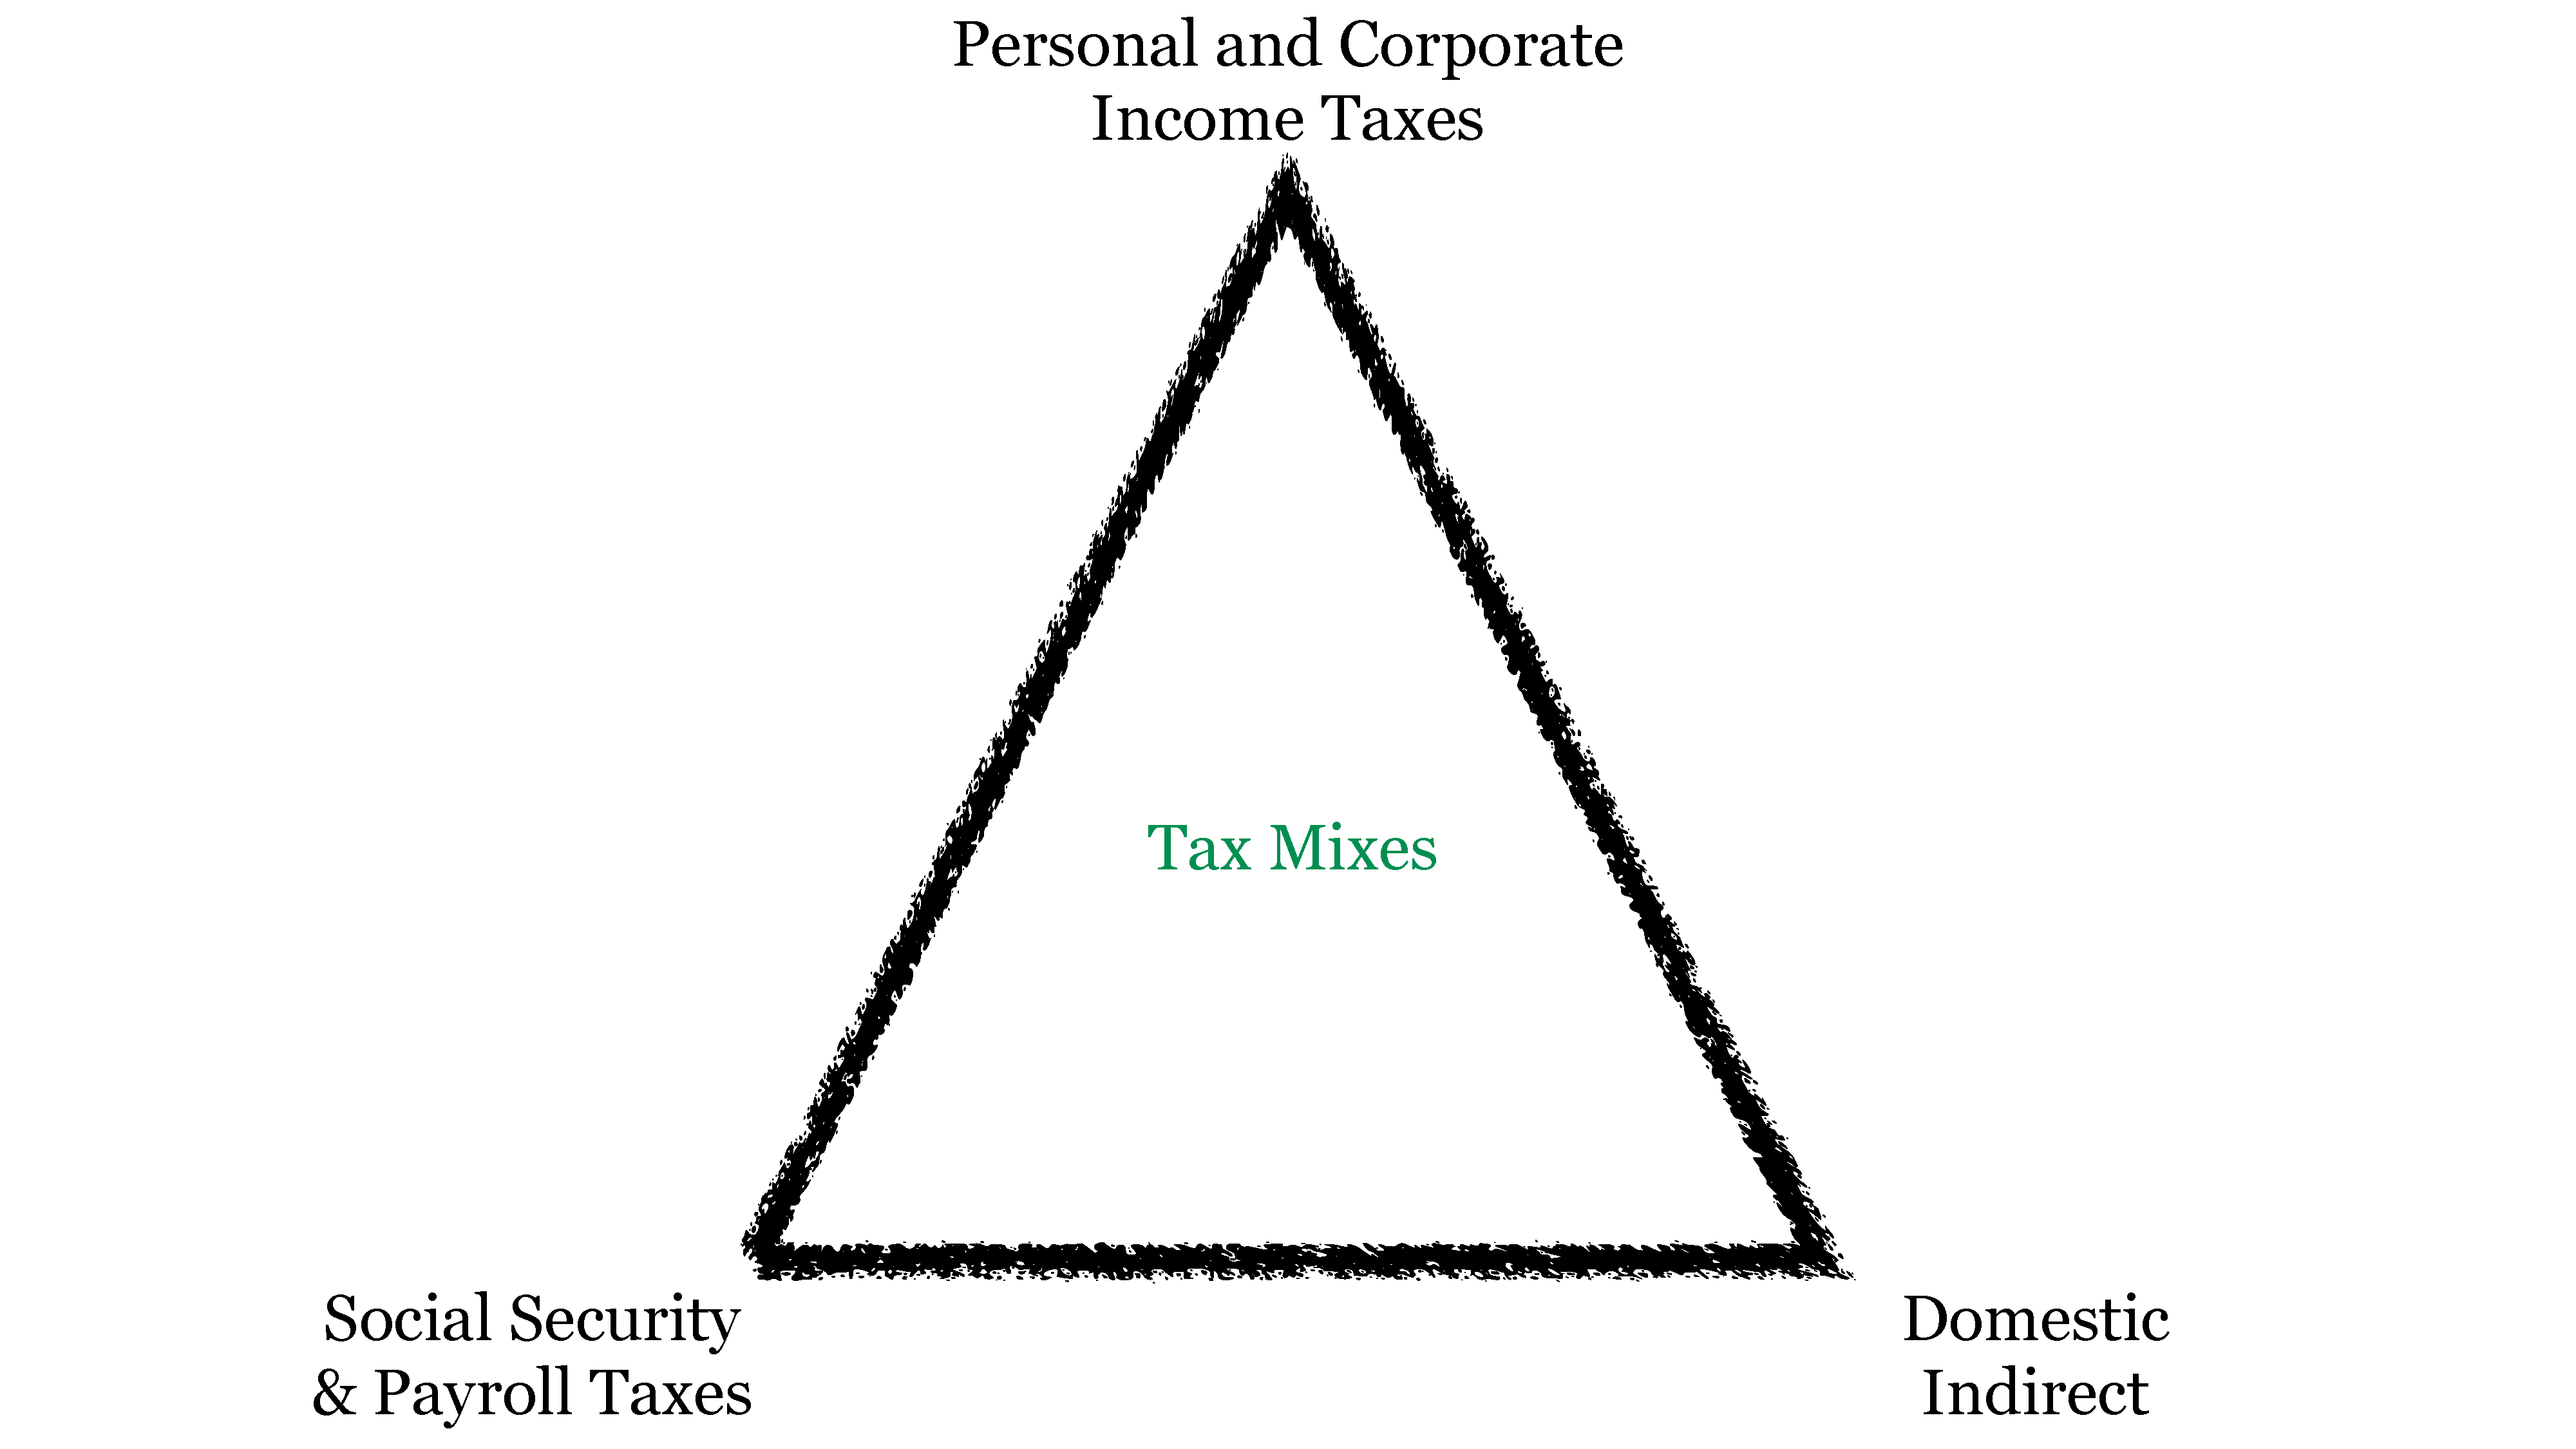
\includegraphics[width=1\linewidth]{tax-mixes}  
	\caption[Tax Mixes]{Tax Mixes of Real Existing Welfare States}
	\label{fig:tax-mixes}
	%somehow link this to the other tax 
\end{figure} 

%here used to be tax-with-trends, it's now in testing-hypotheticals

Designing \hyperref[sec:Desirability]{desirable taxation} in the real world is hard. Economic and administrative complications beset taxation and easily effect undesirable, unintended consequences \citep{Merton-1968-aa}. Economic complications arise where market participants interact with tax policies. Administrative complications arise where transactions become complex, or where axiomatically assumed \hyperref[sec:WorkPlay]{distinctions do not hold} in real life (page \pageref{sec:WorkPlay}).
	%circular wording

\section[Incidence]{Incidence: Doable Taxes Exert Well-Defined Burdens} \label{sec:tax-incidence}
%old title: {\emph{Whom} to Taxed? ---\\Redistributive Taxation is Personal} 

%taxing corporations is stupid: they are, and for good reasons, only virtual entities \cite{Coase1937}
	%actually Coase suggests we shouldn't get into this, we should not favor some ways of organizing cooperation over others ...

%remind people here about natural persons, but that is in fairness.

%taxes should always be in real terms, never in nomal terms. That's studpid otherwise.

Corporate bodies have rightfully been characterized as fictions.
	%source
 The welfare of all these non-natural, private juristic persons ultimately accrues to natural persons as their owners, workers or consumers\footnote{
	Foundations with their earmarked, tax-exempt and free-roaming capital may be a exception to this generalization. The beneficiaries of a foundation's mission may substitute as natural persons to which the foundations welfare --- albeit involuntarily --- accrues.\\A \href{http://maxheld.de/2010/03/27/foundations-may-be-bad/}{critical acclaim} of the political economy, democratic legitimacy and taxation of supposedly benevolent foundations is direly needed but clearly beyond the scope of this thesis.}. 
Equity considerations do not apply at the corporate level\footnote{
	Corporate bodies are, of course, \emph{operative} fictions in their consumption of \href{sec:CommonGood}{Common Goods} and \href{sec:NaturalMonopolies}{Natural Monopolies}. To receive correct price signals, corporate bodies should therefore be subjected to Pigouvian taxes and fees.}.

As per desideratum \ref{des:RedistributionAndRevenueAreOne}, \hyperref[des:RedistributionAndRevenueAreOne]{redistributive and revenue generating taxes are one}. It follows that for both these components:

\begin{desideratum}[Personal Taxation]
	A doable tax falls only on natural persons.
	\label{des:PersonalTaxation}
\end{desideratum}


\paragraph{Love and Marriage\ldots} \phantomsection \label{sec:love-marriage}\nopagebreak
\begin{quote}
	\emph{\ldots Go together like horse and carriage (\ldots)\\*
	Try, try, try to separate them:\\*
	It's an illusion.}\\*\\*
	Frank Sinatra (1915-1998)
\end{quote}
%add triangle of impossibility here
Personal taxation becomes impossible when common usage, transfers and mutual obligations become so intensive, informal and intangible as to render individual accounts meaningless. In modern, functionally differentiated societies such \emph{mechanical solidarity} is --- for better or for worse --- largely replaced by extensive, formalized and tangible \emph{organic solidarity} \citep{Durkheim-1893-aa}. 

%for a more comprehensive discussion of gender and tax, especially its interatcion through class, see \cite{McCaffery2009a}
	%also note that imputed income would provide a partial fix for the problem as in \cite[6304]{McCaffery2009a} 

Romantic cohabitation, marriage and the nuclear family alone remain as refuges of mechanical solidarity. Personal taxation of (married) couples and families becomes impracticable. They are therefore taxed as \emph{one} entity, or at least under one rate. Under \href{des:SharpProgression}{progression} as per desideratum \ref{des:SharpProgression}, a problem arises: you have to add (two) potentially (very) different incomes\footnote{The problem occurs in equivalent form when a different base for progressive taxation is chosen, for example property or consumption.} together and tax them under a \emph{single} rate. There are two ways to do this. First, you can apply the same schedule as for single households, which would punish people just for getting married or having children. For example, two people earning \$50,000 each would, after marriage, be taxed under the higher rate applicable at \$100,000. Secondly, you can divide the family income by the number of people in the household and apply the tax rate for this \emph{average} income. In this case, the tax liability will depend on the \emph{distribution} of incomes \emph{between} the family members. If their incomes are starkly different, they will benefit from applying a progressive rate to their \emph{average} income. This conundrum cannot be resolved: it is the equivalent to \citeauthor{Arrow1950}'s \emph{Impossibility Theorem} in taxation. Of three desirable things, you can only have two: 1) \href{des:SharpProgression}{a progressive schedule}, 2) neutrality towards marriage and 3) tax liability independent of the distribution of income in a household (\citealt{Moffitt2003}: 124; \citealt{Dalsgaard2005}: 29). 
	%add: practical: anything inbetween, but still same problem

I have stated here that \href{des:SharpProgression}{progression} is desirable, and that people should not and cannot be punished for mechanical solidarity in family and marriage. It follows that, while undesirable, the tax liability \emph{will} be dependent on the distribution of income in a household.

The contradictions arising in the taxation of family and marriage point to more fundamental \href{sec:WorkPlay}{problems of drawing boundaries} (page \pageref{sec:WorkPlay}) based on administrative and analytical abstractions (here: \hyperref[des:PersonalTaxation]{taxation of natural persons}, page \pageref{des:PersonalTaxation}) that are not unambiguously applicable in real life. As this particular problem affects all progressive taxes, it will not be further addressed here. 

 The aggregate costs of taxation depend on the responsiveness, or elasticities of what is being taxed. The individual costs --- who \emph{really} pays --- also depend on this responsiveness.

\paragraph{Flypaper Theory is False.} To illustrate this dynamic, first consider \autoref{fig:SameIncidence}. In this market (actually the same as in \autoref{fig:DWL}), a tax is placed on the supplier. For any given market price, the producer is now willing to produce less. The supply curve shifts upwards by exactly the amount of the tax. Assuming constant demand, the curtailed supply will raise the price above the prior equilibrium. Both consumers and producers end up paying for the tax. Consumers have to buy at higher prices. Producers have to sell at lower prices. In this case, consumers and producers carry an equal share of the tax burden\footnote{
	In this illustration, the costs to consumers and producers are only the product of the post-tax quantity and the prices they receive, respectively. In \autoref{fig:DWL} these are the rectangles $B$ and $C$ formed by the price difference to equilibrium prices at post-tax quantities. An equivalent mechanism operates to distribute the burden of the DWL, or the foregone consumption (production) at lower (higher) prices. The DWL is also split evenly between consumers and producers in this case. More generally, the DWL is split according to relative elasticities of supply and demand: whichever is less elastic, bears the greater DWL.  The ``incidence'' of DWLs is customarily not included in assessments of tax incidence, precisely because tax incidence is concerned with the ultimate origin of tax \emph{revenue}. The DWL, by definition, is that welfare lost that is \emph{not} recouped as tax revenue.}.

%this figure is already in mixed economy. It's now fig:same-incidence

The naive ``flypaper theory of tax incidence'' is false: the state cannot easily legislate \href{sec:RedistributionIsPersonal}{who \emph{should} pay} a tax. Instead it must anticipate market reactions to the tax and gauge the \emph{effective} incidence, irrespective of where the tax was originally levied\footnote{
	The usual assumption is that incidence applies only to indirect taxes (VAT, Corporate Income Tax). I find this limited application of incidence implausible. The concept remains applicable for direct taxes (Personal Income Tax (PIT), Asset Tax), too. A PIT on labor incomes, for instance, may partially fall on employers when labor markets are very tight: tax-depressed worker supply may lead employers to pay more. Even an Asset Tax may fall on people other than the owners when demand for their collateral is sufficiently inelastic: interest rates may rise when private capital becomes less abundant. A more complete discussion of the incidence of the different taxes must await \autoref{sec:contest} on page \pageref{sec:contest}.}.
		%really? Asset Tax?

\paragraph{The Relatively Less Elastic Bears Relatively More.} The incidence is not only different from where a tax is levied, it can also fall asymmetrically on demand and supply. More specifically, the incidence of a tax is determined by the \emph{relative} price elasticities of supply and demand: whoever is less elastic (more inelastic) bears a relatively greater share of the burden.

\autoref{fig:DifferentIncidence} illustrates the incidence of a tax on suppliers in a market with relatively less elastic (more inelastic) demand. It is the same market as in \autoref{fig:SameIncidence} and \ref{fig:DWL}, only the elasticity of demand is different: buyers react relatively less to price changes than sellers. As a result, buyers are willing to pay quite a lot to maintain a similar quantity. Sellers, by contrast, will curtail their production substantially when prices drop. The market reaches a post-tax equilibrium at a price much greater than pre-tax equilibrium for consumers, and a little lower for producers. Consumers end up bearing most of the burden.

%this figure is now in mixed economy. fig:different-incidence

%generally, make a big overview of different taxes and taxonomy used here just to make it easier for people to follow. Put it in the appendix.

\paragraph{Incidence is Hard.} As argued in the above, relative price elasticities of demand and supply can be hard to ascertain ex-ante, and they are affected by many factors. To reliably gauge the effective incidence of a tax, government would have to know the elasticities in a myriad of markets and constellations with great precision. This will be very costly and likely unsuccessful.
	%does the PCT really have a good incidence? Think mercedes/daimler
	

To effectively redistribute between \href{des:PersonalTaxation}{natural persons only}, as per desideratum \ref{des:PersonalTaxation}, a doable tax will fall on market interactions where relative elasticities of demand and supply can be easily and reliably ascertained. Government can achieve non-random, normatively justifiable redistribution only when:

\begin{desideratum}[Determined Incidence]
	A doable tax has a well-determined incidence.
	\label{des:TaxIncidence}
\end{desideratum}

\section[Elasticity]{Elasticity: Doable Taxes Hardly Alter Economic Exchanges} \label{sec:tax-elasticity} %{\emph{How} to Tax? ---\\Taxing Inelastic Bases Minimizes DWLs} \label{sec:TaxInelastic} 
Desideratum \ref{des:DWL} holds that \href{des:DWL}{a desirable tax should have a minimal deadweight loss}. A DWL arises when the tax revenue recouped is smaller than the consumer and producer surplus lost as a result of depressed market exchanges or gains from trade (see \autoref{fig:DWL}). A doable tax with a minimal DWL will fall on market exchanges that respond little to the resulting price change. 

\paragraph{Responsiveness is Elasticity.} This responsiveness is called the \emph{price elasticity} of demand and supply respectively. It is defined as the percent change in quantity demanded (supplied) over a percent change in price \citep{Marshall1890}. Where $E-{d}$ ($E-{s}$)  is the price elasticity of demand (supply), $Q-{d}$ ($Q-{s}$) the quantity demanded (supplied) and $P$ the price, it holds that:

	\begin{equation} \label{eq:PED}
			E-{d}=\frac{\%\ \mbox{change in quantity demanded}}{\%\ \mbox{change in price}}=\frac{\Delta Q-{d}/{Q-{d}}}{{\Delta P}/{P}}
	\end{equation}

 and
 
 	\begin{equation} \label{eq:PES}
			E-{s}=\frac{\%\ \mbox{change in quantity supplied}}{\%\ \mbox{change in price}}=\frac{\Delta Q-{s}/{Q-{s}}}{{\Delta P}/{P}}
	\end{equation}.

\paragraph{Elasticities of Supply and Demand} become more intuitive when applied in polar cases of \href{fig:Inelastic}{perfect inelasticity} (\autoref{fig:Inelastic}) and \href{fig:Elastic}{perfect elasticity} (\autoref{fig:Elastic}). 

%I definetely NEED to look into the Harbinger triangle literature on the costs of taxation. This seems to be different from this (Marshallian?) view based on consumer surplus. There's also a view based on (Pigou?), asking whether the loosers (the taxpayers) can be compensated by the winners (the recipients of subsidies).

\subparagraph{Perfectly elastic} supply (demand) does not respond at all to changes in price. Whatever the price, suppliers (buyers) will always produce (buy) the same quantity. It is displayed by a perpendicular supply (demand) curve in \autoref{fig:Inelastic}.

\subparagraph{Perfectly inelastic} supply (demand) responds maximally to minimal changes in price. When the price drops (rises) below a certain point, suppliers (buyers) will cease stop producing (buying) any quantity. Below (above) the horizontal supply (demand) curve in \autoref{fig:Elastic}, no production (buying) occurs at all.
 
 \begin{figure}[htbp]
	\centering
	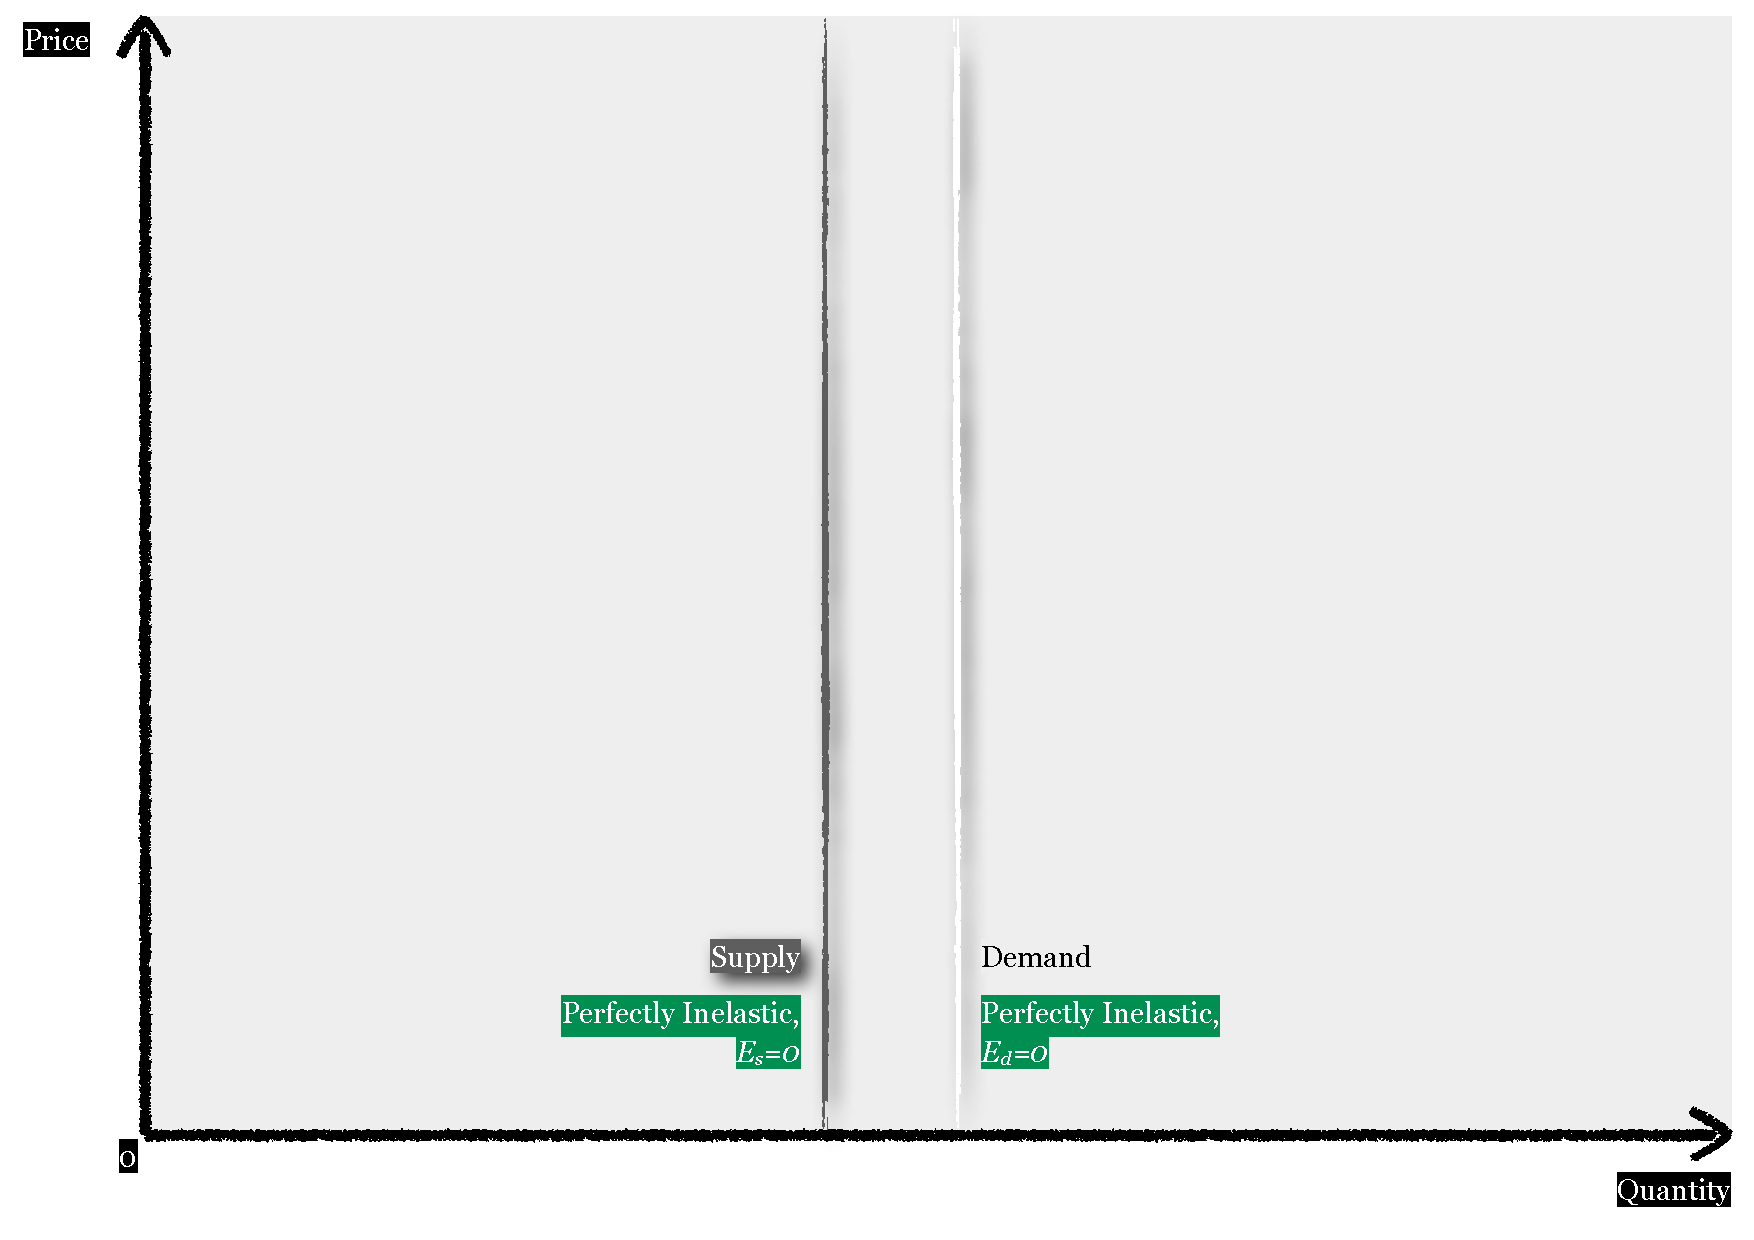
\includegraphics[width=1\textwidth]{inelastic}  
	\caption{Perfectly Inelastic Supply and Demand}
	\label{fig:Inelastic}
\end{figure}
 
 \begin{figure}[htbp]
	\centering
	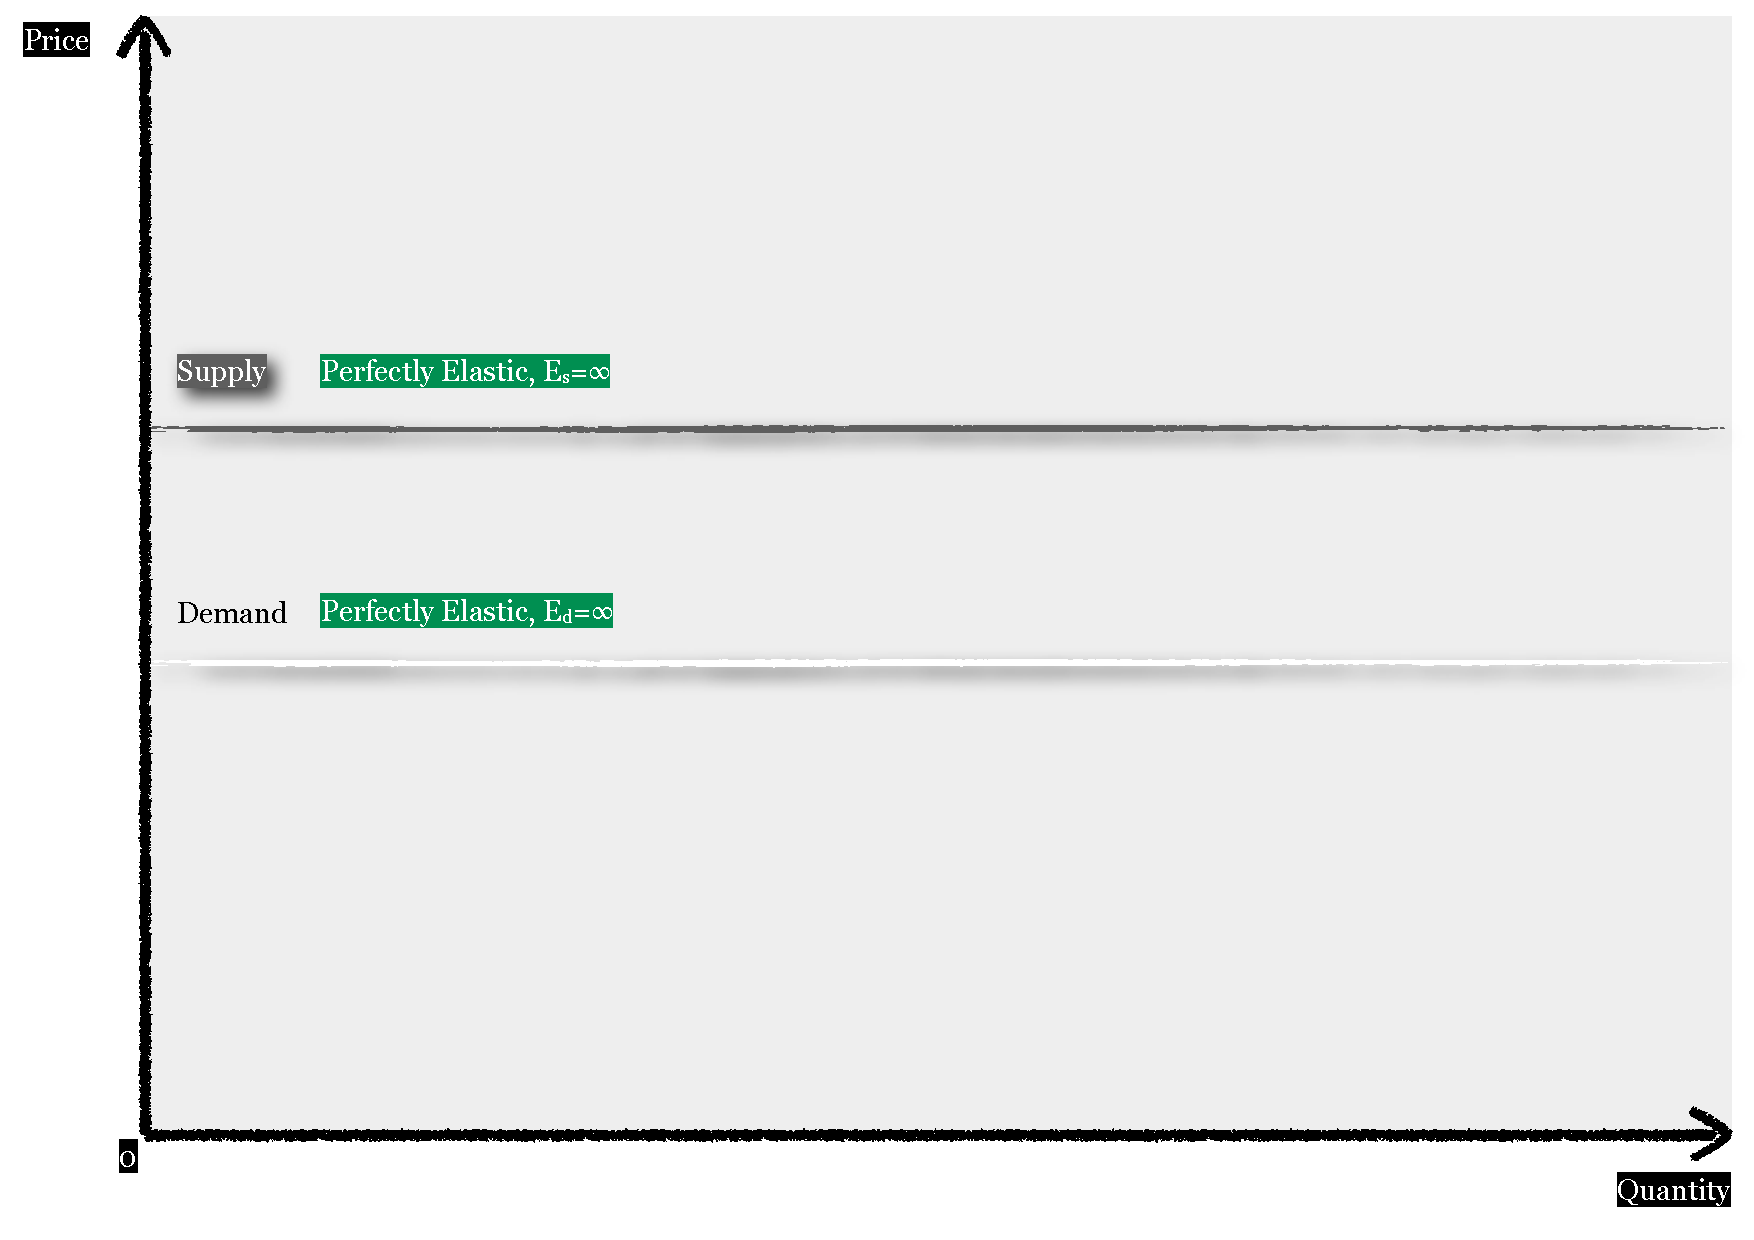
\includegraphics[width=1\textwidth]{elastic}  
	\caption{Perfectly Elastic Supply and Demand}
	\label{fig:Elastic}
\end{figure}

 \begin{figure}[htbp]
	\centering
	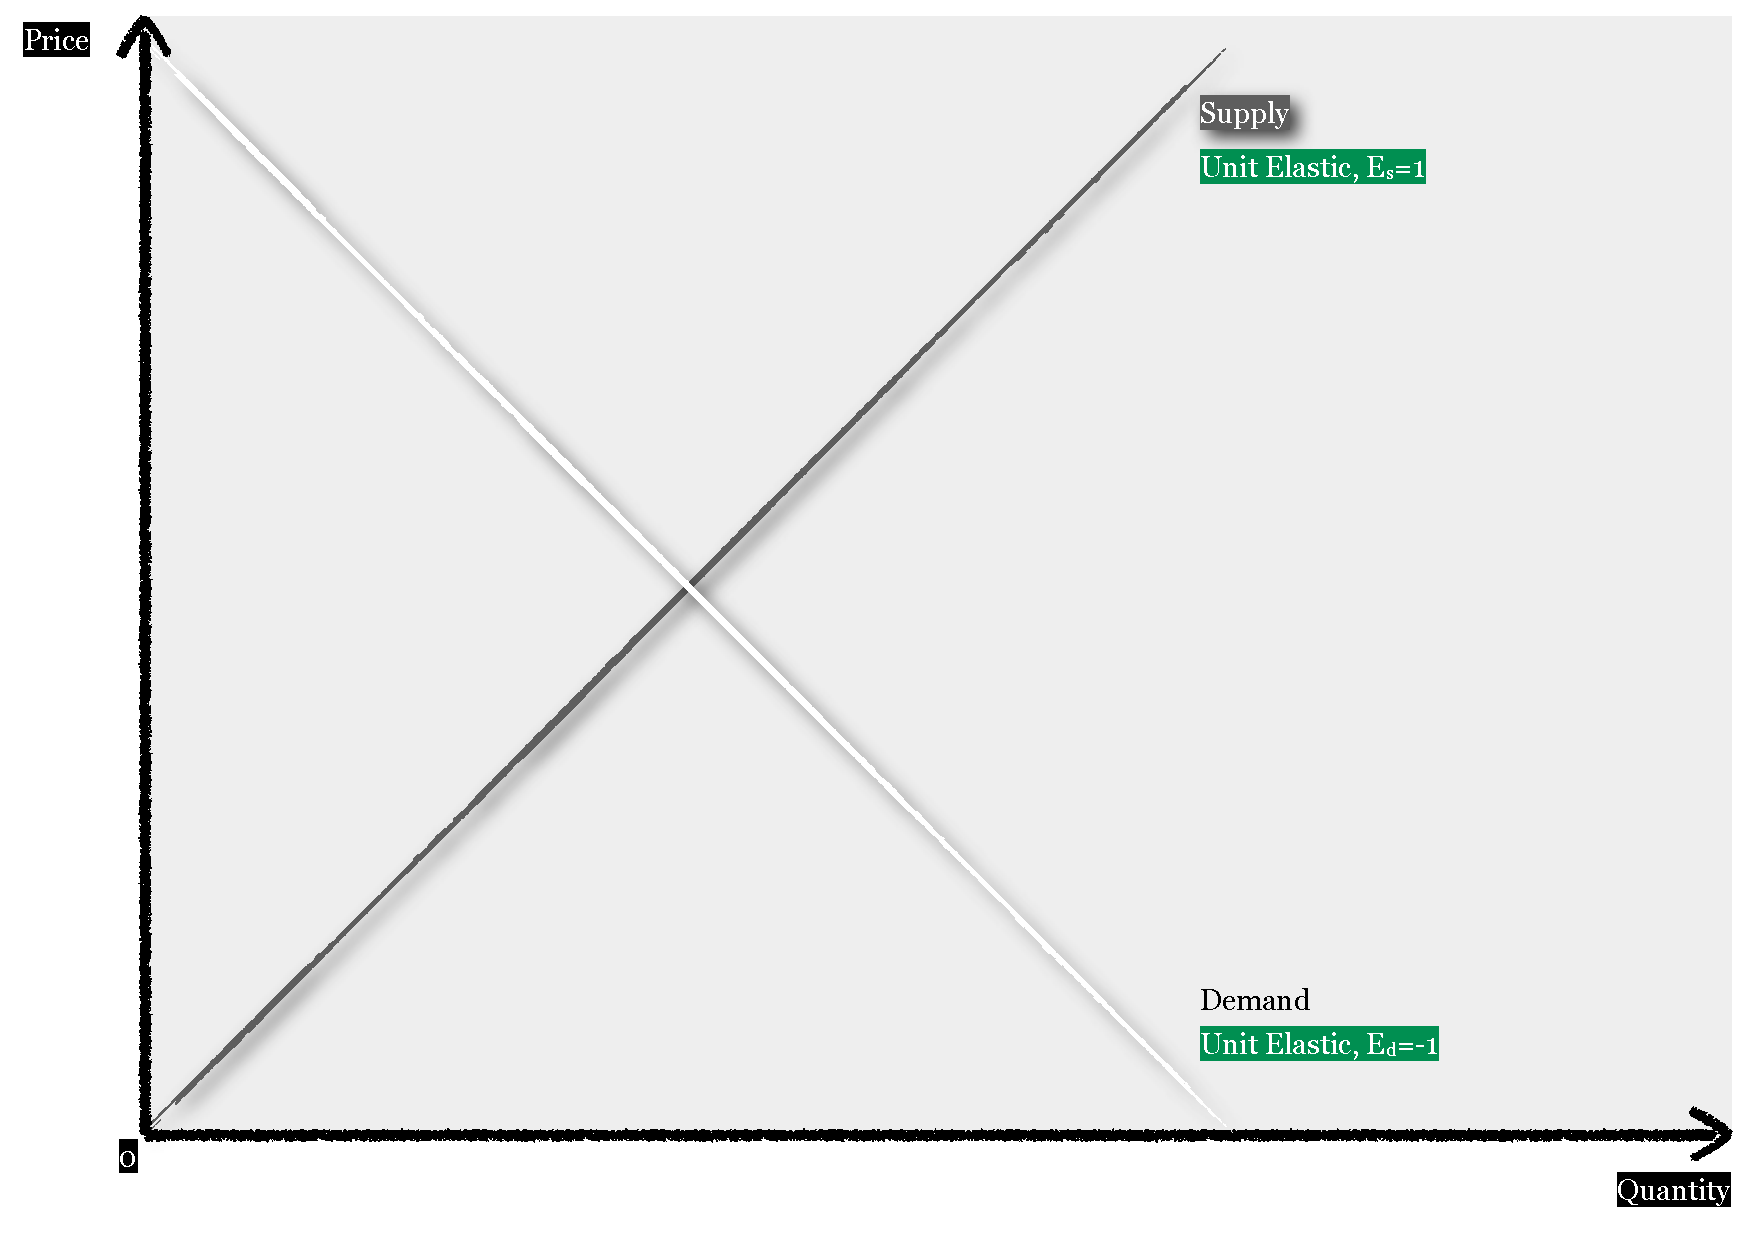
\includegraphics[width=1\textwidth]{unit-elastic}  
	\caption{Unit Elastic Supply and Demand}
	\label{fig:UnitElastic}
\end{figure}

\subparagraph{Unit elastic} supply (demand) responds proportionally to changes in price. Along a supply (demand) curve of slope $1$ ($-1$), producers (buyers) produce (buy) one percent more quantity for each percent increase (decrease) in price\footnote{The complications of point-vs.-arc elasticities are of no relevance here. For a review, see \cite{Allen1933} and recently, \cite{Vaughan1988}.}.

\paragraph{Elasticities and DWLs.} Because DWLs stem from market participants tax-depressed activity, less price responsive activities will be more efficient to tax. Relatively inelastic supply and demand will have relatively smaller DWLs (\citealt{Ramsey}, \citealt{Piatkowski2008}: 16). 

%this figure is now in mixed economy \label{fig:smaller-DWL}

This is illustrated in figures \ref{fig:DWL} and \ref{fig:smaller-DWL}. \autoref{fig:smaller-DWL} displays the same market with the same tax, only with relatively less elastic (= more inelastic) supply and demand. Compared to the original DWL-scenario in \autoref{fig:DWL}, the DWL in \autoref{fig:smaller-DWL} is absolutely smaller and smaller relative to the recouped tax revenue. Because both producers and buyers are less responsive to the tax-induced price change, they each loose less of their surplus.

A doable specification of desideratum \ref{des:DWL} on \href{des:DWL}{minimal DWLs} is:

\begin{desideratum}[Tax Inelastic Bases]
	A doable tax falls on inelastic bases.
	\label{des:tax-inelastic}
\end{desideratum}

\paragraph{Determinants of Elasticity.} Elasticities are hard to quantify: if prices change, they typically change only marginally. Elasticities are typically known only \emph{locally}, that is, in the vicinity of equilibrium prices.

Elasticities are determined by a host of factors. The price elasticity of supply depends, amongst other things, on the mobility of labor and capital employed in production, the availability of substitute consumers or the ability to substitute current for future sales (a.k.a. liquidity). The price elasticity of demand depends, amongt other things, on the availability of substitute goods, brand loyalty or ability to substitute current for future consumption.

\section[Schedule]{Schedule} \label{sec:tax-schedule}
%cold progression
%make it smooth, just what must the curve be?
%the first derivative must never be ...

%maybe mention here the boundaries on which taxation depends?

\section[Timing]{Timing: A Doable Tax Falls on Liquid Goods} \label{sec:tax-timing} %worry: is this maybe yet another subset of a DWL problem?
%old title: when to tax: measuring economic flows is non-trivial

\subsection{Savings norms}

%does this belong here?
%include here the visualization from McCaffery, note that it is an application of Modigiliani's Life Cycle Income Hypothesis (Wikipedia) (original source is unclear)

\subsection{Liquidity}

%get quote

% via wikipedia on LVT, here's a reason for why govntm evaluation is always bad: Austrian School economist Murray Rothbard later raised similar concerns, stating that no government can fairly assess value, which can only be determined by a free market.[20]
	%Rothbard, Murray. "The Single Tax: Economic and Moral Implications and A Reply to Georgist Criticisms". The Mises Institute. Retrieved 2009-02-13.
	
Any non-flat distributive norm of taxation requires that \emph{ability to pay} (or some other criterion) is measurable.   In a non-static economy, this ability will change over time. It is hard to know exactly \emph{when} welfare accrues to people and can be even harder to measure.

\paragraph{The Good: Exchanges.} In perfect, liquid markets exchanges are so frequent, intensive and transparent that the equilibrium valuation of  buyers and sellers can be known at every time and with great precision. Stock exchanges are a good example: company stocks are bought an sold so often, by so many people, and so publicly that at every second during the trading day, the current valuation of a company is known with the greatest possible accuracy, reflecting all past publicly available information (this according to the efficient market hypothesis (EMH), originally stated by \citealt{Cowles1937}). If you own stock, the taxman can determine the welfare losses and gains that accrue to you on any given day, even without you ever selling your share of a company.
	%homogeneous goods of same quality
	%consider debt vs equity finance in this
	%also its about liquidity not necessarily welfare

\paragraph{The OK: Frequent Buying and Selling.} Exchanges do not exist for all goods and services in an economy. An equilibrium valuation for many things is reached only when, and if they are bought and sold. 
This is relatively unproblematic for things that are bought an sold relatively often, such as labor. In labor markets, the taxman can simply assume that the welfare of your human capital accrues to you only when the first salary is transferred, even though this is probably incorrect. Your value as a trained worker, after all, did not accrue to you over night, but was (l)earned over many years. 

\paragraph{The OK: Standardized Goods With Great Volume.} Even without \emph{individually} frequent buying and selling, equilibrium valuation is possible when goods and services are easily comparable and bought and sold by \emph{someone}. Used cars, for example, can be easily evaluated because their quality is comparable in terms of standardized features\footnote{\ldots even though the quality may not be symmetrically observable in this, \citeauthor{Akerlof-1970-aa}'s (\citeyear{Akerlof-1970-aa}) proverbial lemon's market.} and someone, somewhere will sell a same or similar car most of the time. All the taxman\footnote{\ldots or, in Germany, a private service by the name of \href{http://www.schwacke.de/}{Schwacke}, in the US \href{http://www.kbb.com/}{Kelly Blue Book}.} has to do is to record all the equilibrium prices, and he can quantify just how much better off you are, once you have inherited your grandmothers car, even if you do not plan on ever selling it.

\paragraph{The Bad: Illiquid Markets of Unstandardized Goods.} Sadly for the taxman, some goods are hardly ever traded and are of unstandardized quality, such as large real estate or privately owned companies. Not only is no valuation of these things publicly known, it simply is not defined: just how much that mansion or family enterprise is worth \emph{cannot} be known unless and until it is sold. 

\paragraph{The Ugly: Flight Into Illiquid Markets.} \phantomsection \label{sec:FreezingUp} Things can get even more ugly, when taxpayers anticipate the state's inability to tax welfare accrual in illiquid markets and react accordingly. Taxpayers can have several incentives to ``hide'' their welfare accrual in illiquid markets. First, under \href{des:SharpProgression}{progression}, as per desideratum \ref{des:SharpProgression}, taxpayers have an incentive to smooth out their welfare accrual over time. Second, given that we all die, taxpayers have an incentive to postpone taxation of their welfare accrual until after they are dead, or even into the farther future after their children's death. This is not an esoteric or theoretic problem: given the large properties handed down for generations in the form of real estate or privately owned companies, a substantial part of material inequality in our societies will escape taxation, at least under a humanly meaningful time horizon. Thirdly, and most sinisterly, taxpayers can follow the strategy of ``\href{sec:Evasion101}{tax evasion 101}'', \emph{buy} illiquid goods, \emph{borrow} and spend on them as collateral and \emph{die} before the illiquid good is ever sold.

When taxpayers \emph{do} react to these incentives and buy illiquid assets, they will not only evade redistribution, but they will also cause substantial welfare losses. When, for example, many taxpayers decide to invest in real estate, rather than company stock, equity markets may lack that very capital that they could put to potentially more \emph{socially} productive use. Even worse, when the owner of an inherited family SME avoids a merger or acquisition for fear of taxation (the firm \emph{could} be evaluated after the M\&A deal), \href{sec:PerfectCompetition}{perfect competition condition} {itm:EasyEntry} (\hyperref[itm:EasyEntry]{easy entry and exit}) is violated, and at least one invisible hand of the free market is tied behind our backs. In the worst case, originally liquid markets will freeze up as more taxpayers postpone their selling into the indefinite future\footnote{The catastrophic welfare effects of freezing-up of illiquid markets could recently be observed during the 2007-2010 financial crisis, when banks, for fear of bad risks (not taxation) ceased to evaluate each other and stopped lending each other money overnight.}.

\paragraph{The Unavoidable: Illiquid Goods.} It is important to note here, that for all their tax-hassle, ``naturally'' illiquid assets such as privately owned firms are not an avoidable aberration of efficient markets. Rewards of private information and unobservable effort in the form of such illiquid assets are in fact a necessary condition for an innovative market economy. An economy in which \emph{all} privately known but uncertain information would immediately be made public and evaluated (decided upon) on an open exchange is, essentially, a planned, if democratic, economy.
	%note arrow information
 Two problems would arise. First, the universal exchange would underestimate the value of goods that are produced with uncertain innovation and unobservable effort, precisely because the stochastic value of such goods is initially low. Second, people would have little incentive to invest maximum unobservable effort and uncertain innovations in the first place, because the universal exchange would prevent them from ever obtaining any above-average returns on their new product. Had Sergey Brin and Lawrence Page of Google Inc. been forced to publish and evaluate their innovative search algorithm during every state of its development, they would have had limited incentives to start hacking code in the first place. The careful timing of initial public offerings (IPOs) of technology startups also reflects this fundamental capitalist contradiction between efficient markets (EMH) and incentive design\footnote{
	For a recent commentary on the same contradiction in the governance of rating agencies, see \citealt{TheEconomist2009}. Rating agencies, like tech entrepreneurs need incentives to come up with clever algorithms in the first place. At the same time, EMH demands that all information (and the technology to analyze it) be made public immediately.}.

\paragraph{Between a Rock and Hard Place: Taxation on Accrual or Realization.} Governments have two equally poor choices to tax illiquid goods. They can either tax on \emph{accrual} or on \emph{realization}.

\subparagraph{On Accrual.} To tax on \emph{actual} accrual, government has to evaluate an illiquid good in the absence of \emph{any} market evaluation. Two problems arise. First, by creating an evaluation and consequent incentives out of mid-air, government becomes a central planner. Second, the evaluation itself will put extraordinary strain on the political process. 
	%rentier economy read reference this stuff
Absent any objectifiable basis or normative justification for government evaluations, it will be hard to insulate the political process from corruption in these zero-sum games between different goods, owners and the state. A publicly accountable administration evaluating two equally illiquid family-owned firms every year will be under tremendous pressure from both owners, as well as everyone else who does not own either of the two firms. %Austrian school economist murry rothbard argued that government cannot fairly assess value, only markets can do that. This is in "the single tax" economic and ... implications, a reply two my georgist criticism.

\subparagraph{On Realization.} To tax on realization, government has to wait until eventually, an illiquid good \emph{is} sold at an equilibrium price. Again, two problems arise. First, effective taxation may be postponed beyond a humanly meaningful timespan. Secondly, as argued in the above, taxation on realization can cause taxpayers to \href{sec:FreezingUp}{flee into illiquid markets and to freeze up previously liquid markets}. 

There is no good way to tax accrual in illiquid assets. Exempting illiquid assets from taxation alltogether will lead to the same problems as taxation on realization: even more taxpayers will shelter their accrual in illiquid goods.

The evaluation of illiquid assets may in some instances be as unavoidable as illiquid goods themselves. Banks do it when they establish collateral for a loan or when they assess the creditworthiness of a privately-owned firm\footnote{One may be tempted to believe that the state should be able to evaluate illiquid assets because banks do it, too. This misconstrues the extension of credit by a bank. The evaluation of collateral by a bank is of course an \emph{equilibrium} valuation, albeit one that is (hopefully) never cashed in. Borrowers can go to a different bank to seek a higher valuation. Lenders can turn away creditors if they seek a lower valuation. Citizens cannot go to another tax administration to get another evaluation of their illiquid good. They have only one state.}. States may have to do it in taxation. Still, whenever possible, states should avoid messing with this (productive?) contradiction inherent to the capitalist mode of production:

\begin{desideratum}[No Illiquid Assets]
	A doable tax will fall on liquid assets. %is it possible that what I mean here is not liquidity, but cashflow?
	\label{des:NoIlliquidAssets}
\end{desideratum}

\section[Neutrality]{Neutrality: A Doable Tax is Neutral to Economic Behavior} \label{sec:tax-neutrality}

\subsection{Work vs. Leisure}

%maybe include free time here, too?

%add some stuff from Fullerton et al 1983 (it's already read and highlighted). In particular, stress the importance of imputed income to alleviate the work/leisure bias.. There's also a 1973 dollar figure for the PCT: 500-600 billion dollars, or 975-1.3 trillion. Read this again. Consider carefully what this models.

\subsection{Capital vs. Labor} %{\emph{What} to Tax? ---\\Capital vs. Labor Incomes} \label{sec:CapitalLabor} 

\subsection{Capital} 
Much of the debate on taxation in recent years has concentrated on the relative taxation of capital and labor. This dichotomy is no longer \href{sec:CapitalNoClass}{empirically meaningful}, and \href{sec:TwoSavingsNorms}{normatively contradictory}.

\paragraph{Empirically: Marxism is Dead --- Capital is no Longer a Class in Itself.} \phantomsection \label{sec:CapitalNoClass} For \href{des:PersonalTaxation}{personal taxation} as per desideratum \ref{des:PersonalTaxation}, capital and labor incomes are an irrelevant, false dichotomy. Today, capital is no longer a class in itself: even middle class earners have substantial capital incomes, for example from capital-based pensions or life insurances (\citealt{Grabka2007a}: XV). In a (happily) past world of bifurcation between workers and capitalists, balancing the taxation of labor and capital incomes made redistributive sense. When almost everyone is, to some extent, a capitalist, taxation of either of the two incomes does not neatly map on \hyperref[des:PersonalTaxation]{natural persons} (page \pageref{des:PersonalTaxation}). \emph{Any} tax mix of labor and capital incomes will have indeterminate redistributive effects.

\paragraph{Normatively: Two Savings Norms Conflict.} \phantomsection \label{sec:TwoSavingsNorms} Capital, in the last instance, is saved labor income. There are two conflicting, equally plausible norms on how to treat saving.

\subparagraph{Ordinary Savings Norm.} \phantomsection \label{sec:OSN} According to the ordinary savings norm, people save to shift labor incomes within their lifetime, or between generations (\citealt{McCaffery2005}: 819). They receive a return to capital to make up for the the risk borne and the \hyperref[item:Uncertainty]{pure discount of the future} (*{item:Uncertainty}). Because the saver and the non-saver are same ex ante, they should not be taxed differently ex post. In short, people should not be punished to smooth out their consumption over time.

\subparagraph{Yield-to-Capital Norm.} \phantomsection \label{sec:Y2C} According to the yield-to-capital norm, the return to capital that people receive is additionally accumulated welfare that should be taxed. 

Under income taxation, these two norms are in fatal tension. \emph{Any} mix of capital and labor income taxation will violate either of the two norms. There is no meaningful way to tell the one kind of (ordinary) saving from the other (yield) kind: they are the two sides of the same coin.

%add somewhere: how resilient are taxes to fraud (new des)

\paragraph{Structural Agnosticism.} A tax regime can avoid this empirical futility and normative contradictions when it is agnostic in its treatment of labor and capital incomes:

\begin{desideratum}[Agnostic Towards Labor and Capital Incomes]
	A doable tax will be agnostic towards labor and capital incomes.
	\label{des:structural-agnosticism}
\end{desideratum}
	%also note that the PCT's evil twins, including FairTax USA-Tax X-Tax do NOT include this.

%via session report for econ governance. When done, copy/paste me to thesis(!!)

	\chapter[Better Tax]{A Better Tax}
		\label{chap:better-tax}
		%! TEX root=../tax-n-democracy-held.tex

\chapter[Better Tax]{A Better Tax} \label{chap:better-tax}

%add comments, footnote: this was first submitted as ...

\begin{quote}
	\emph{``Yes we can: to justice and equality. Yes we can: to opportunity and prosperity.''}\\*
	--- Barack H. Obama, Obama For America 2008
\end{quote}

\section{The Contestants} \label{sec:contestants} Which taxes exist in the real world, and which taxes are conceivable? It will not be possible to list them all here in all their legal and administrative detail. Instead, rough archetypes of real existing taxes (VAT, Payroll, (Dual) PIT, CIT, Local Business Tax) will serve to compare them to the three hypothetical (or rare) taxes suggested (PCT, Wealth Tax, NIT).

%also explain the distinction of indirect taxes here, because I don't use that in the following, it's more analytic than that.
	
%here used to be the tax-overview thing, it's now in testing-hypotheticals

\begin{figure}[htbp]
	\centering
	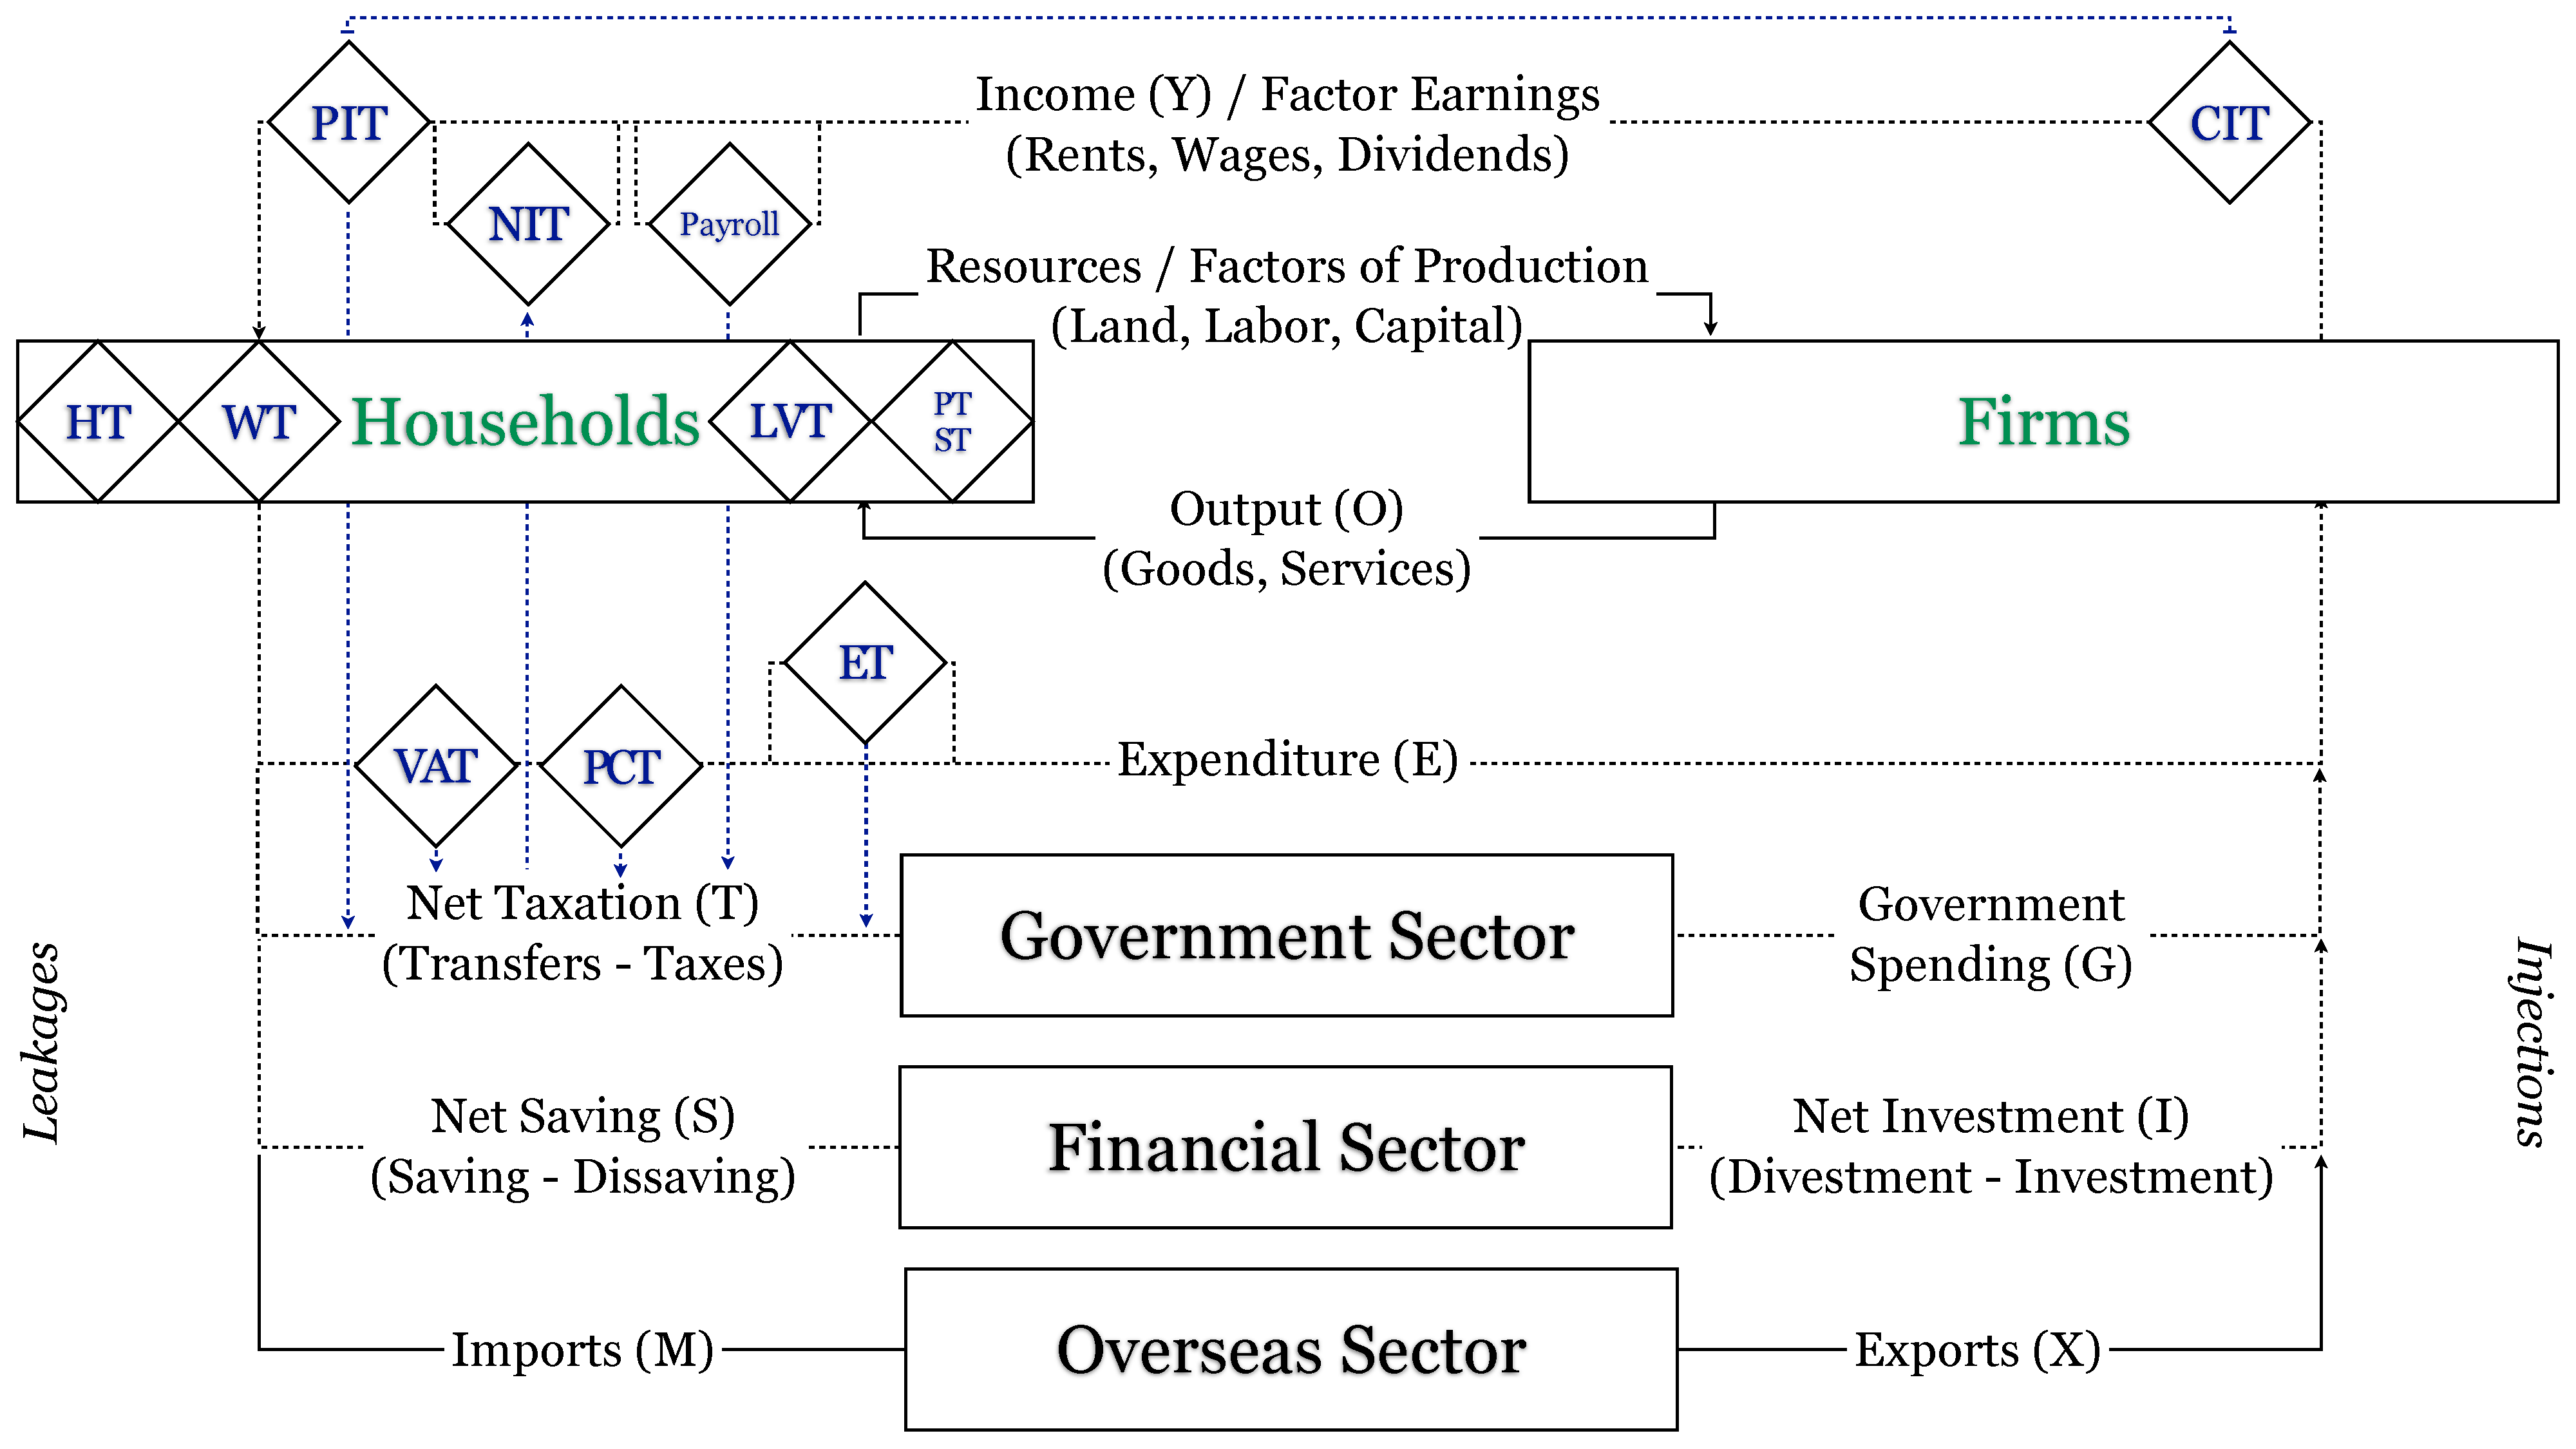
\includegraphics[width=1\textwidth]{circular-flow-with-taxes}  
	\caption[Circular Flow in the Economy, with Taxes]{Circular Flow of Income in the Economy, with Tax Revenue Sources}
	\begin{flushleft}
		\scriptsize{Compare \autoref{fig:circular-flow}.}
		%!TEX root=../tax-democracy-held.tex

\scriptsize{
	\glsfirst{CIT},
	\glsfirst{Dual-PIT},
	\glsfirst{Ecotax},
	\glsfirst{ET},
	\glsfirst{FTT},
	\glsfirst{LBT},
	\glsfirst{LVT},
	\glsfirst{NIT},
	\glsfirst{OSN},
	\glsfirst{PCT},
	\glsfirst{Payroll},
	\glsfirst{PT},
	\glsfirst{SD},
	\glsfirst{VAT},
	\glsfirst{WT},
	\glsfirst{Y2C} and

	\hyperref[sec:distributive-effects-of-inflation]{the distributive effects of in- and deflation} (p.~\pageref{sec:distributive-effects-of-inflation}).
}
	\end{flushleft}
	\label{fig:circular-flow-with-taxes}
\end{figure}
%comment on the extra loops for some taxes

Enter the contestants.

\subsection{Head Tax}

\subsection{Taxes on Income}

\subsubsection{Taxes on Capital Income}

\paragraph{Corporate Income Tax (CIT)} \phantomsection \label{sec:CIT} The \glsreset{CIT} \gls{CIT} taxes the earnings\footnote{In Germany, earnings after interest, depreciation and amortization.} of an incorporated firm. It is usually proportional. Unincorporated firms do not pay \gls{CIT}, instead their owners owe \gls{PIT} on their business earnings\footnote{
	When a corporation hands out a dividend, the dividend is also \gls{PIT}ed. In some jurisdictions, \gls{CIT} is deductible from the \gls{PIT} on dividends. No taxation of dividends applies when the recipient is another corporation.}.
%Graetz 1979: 1635 makes my key point: the one reason for CIT is that "undistributed corporate income does not escape taxation"
	%abolish business taxation (1636)
	%a corporation has no one "ability to pay"

\glspl{CIT} are proportional, with rates around 20\% in the EU. Countries have recently created issued sectoral (trade, finance) or regional (Hong Kong, London) exemptions from the \gls{CIT} to attract investment \citep{Genschel2009,Ganghof2007,Genschel2005}.

\subparagraph{Local Business Tax (LBT)} \phantomsection \label{sec:LBT} Taxes on local businesses exist only in some OECD countries, including Germany. In Germany, local authorities can tax local business a progressive tax on their earnings. Local authorities set the rate of the tax (within federally mandated margins). Firms are taxable based on the location of their establishments. Earnings of firms with multiple establishments are weighed by the sum of wages and salaries paid.

\subsubsection{Taxes on Capital and Labor Income}

\paragraph{Personal Income Tax (PIT)} \phantomsection \label{sec:PIT} Under the \glsreset{PIT} \gls{PIT}, all sources of personal income (labor, capital) are added and taxed under a single schedule. \gls{PIT} schedules are typically progressive. Marginal (not average!) tax rates in Germany range from 14\% to 42\% (Bundesministerium f\"ur Finanzen 2009). 

	%The personal income tax is usually levied according to a progressive schedule both on labor and capital income. Its incidence is borne by the taxed individual, but it disincentivizes work and (risky) investment. It taxes capital twice: once when it is initially earned and again when it generates an interest. Income taxes only on labor (payroll tax, social contributions) can contribute to structural unemployment by raising effective price floors, especially when they are not sufficiently progressive.

	%Personal income taxes on capital (... gains tax) necessitate a corollary taxation of corporate income. Without it, taxpayers could easily evade payment by incorporating capital it in a firm, withdrawing earnings only slowly. Corporate income tax rates spill over to personal (capital gains) tax rates (Ganghof & Genschel 2008, Ganghof 2006). Like the personal income tax, they depress economic activity.
	%Moreover, corporate income taxes are indeterminate with regard to incidence and flat in their progression. The tax incidence in a firm on either labor or capital is determined by a host of firm- and market-specific factors, including the relative factor price elasticities. Corporate income taxes apply one rate over all shares. The lifesavings of a worker, invested in a company through her life insurance, are taxed at exactly the same rate as the share of a stock-market tycoon.
	%As the base of the corporate income tax is relatively mobile (compared to labor, consumption), it can easily evade taxation or compete down rates.
	

\subparagraph{Dual Income Tax (Dual PIT).} \phantomsection \label{sec:Dual-PIT} \glsreset{Dual-PIT} The \gls{Dual-PIT} is a variation on the \gls{PIT}, where schedules differ between capital and labor sources of income. \glspl{Dual-PIT} burden capital relatively less than labor incomes. The \glspl{Dual-PIT} was introduced to avoid the negative growth effects of high capital taxation (particularly through its \hyperref[sec:CIT]{CIT backstop}, p.~\pageref{sec:CIT}) and to counteract capital flight. 

In Sweden, a pioneer of the \gls{Dual-PIT}, the top marginal (not average!) rate for labor incomes is 55\%. Capital incomes are taxed proportionally at 30\% (marginal rate equals average rate). %add reference

\subsubsection{Taxes on Labor Income}

\paragraph{Payroll Taxes (Payroll)} \phantomsection \label{sec:Payroll} In Germany, and many other countries, social contributions for old age, health, unemployment and long term care insurance are implemented as payroll taxes. Payroll taxes are paid on labor income. Whether they are implemented as withholding taxes (the employer withholds and transfers the tax) or paid out of the employees funds is of no significance here: it does not matter for \hyperref[sec:TaxIncidence]{tax incidence} (page \pageref{sec:TaxIncidence}). 

\subparagraph{Social Insurance Contributions} \phantomsection \label{sec:SIC} are capped \glsreset{Payroll} \gls{Payroll}, actually. Despite this terminological confusion and their administration in semi-independent public agencies, it is important to note that social contributions are government revenue, irrespective of their quasi-fiscal status. Social contributions are \hyperref[sec:PurposesOfTaxation]{proper taxes} (page \pageref{sec:PurposesOfTaxation}). To the extent that government adopts universal provision of health care, unemployment insurance and long term care as allocative goals, compulsory contributions to these services are \hyperref[sec:Redistribution]{redistributive taxes}. To the extent that government finances old-age pensions out of current incomes, such PAYGO contributions are intertemporally and intergenerationally \hyperref[sec:Redistribution]{redistributive taxes}\footnote{
	Payments into capital-based pension schemes are not straightforwardly taxes. Government may however choose to mandate or subsidize such payments to increase the savings rate. As per desideratum \ref{des:Savings} (\hyperref[des:Savings]{arbitrary savings rate}, page \pageref{des:Savings}) such a market intervention \emph{would} be a proper tax, too.}. 
To the extent that private markets for health care, unemployment and long term care insurance are plagued by lemons markets \citep{Akerlof-1970-aa}, respective contributions serve to \hyperref[sec:RiskPooling]{pool risks} (page \pageref{sec:RiskPooling}) and are proper revenue-generating taxes. Additionally, universal health care provides \hyperref[sec:PublicGood]{public good} provision against epidemics (think vaccinations) and unemployment insurance serves as an \hyperref[des:AutomaticStabilizer]{automatic stabilizer} (page \pageref{des:AutomaticStabilizer}) to smooth out economic growth.

Social insurance contributions are presented here for the sake of completion and clarification. They are, when typically implemented as payroll taxes, a variation of a \gls{Dual-PIT}. 

Rates for social insurance contributions are usually proportional. In the EU, they vary from 20\% in Denmark to 32\% in Germany and 50\% in France (Statistisches Bundesamt Deutschland 2007). In Germany, contributions are capped above a certain income threshold, above which additional income is not taxed.

\subsection{Taxes on Consumption}

%what about the distinction about INDIRECT taxes. Indirect taxes are taxes levied on entities other than those expected to bear the eventual burden.

\subsubsection{Prepaid Consumption Taxes}

\paragraph{Value Added Tax (VAT)} \phantomsection \label{sec:VAT} The \glsreset{VAT} \gls{VAT} is best understood as an elegant advancement of a retail sales tax. %best example for a prepaid consumption tax is VAT, in the american context sales taxes
A retail sales tax charges sellers a fixed percentage of the sales price on goods for which the (corporate or private) buyer is the end user. Because under a sales tax, the tax on any single taxable transaction is very high, incentives to evade the tax and to smuggle goods are great. What is more, the state looses \emph{all} tax revenue on a given good when evasion occurs.

%The value-add tax (VAT) is a straightforward indirect tax. It has a relatively immobile base (consumption of everyone), supposedly robust revenues, and is relatively incentive-neutral.
	%The VAT is, however, regressive (poorer people spend more of their income generating capacity on consumption). Like payroll taxes, the VAT raises effective price floors of labor when socially acceptable minima are present, and can thereby contribute to structural unemployment.It emerges from this simplified overview that taxes with progressive schedules also tend to have relative mobile bases#. If mobile tax bases erode relatively more because of tax competition, so will progressive schedules.

The VAT was developed to address this problem. Instead of charging sellers only at the end of a production chain (before the good is consumed), sellers are charged a percentage of their sales prices on \emph{all} goods, including investment and intermediary goods. Sellers invoice the tax to buyers. Buyers are then eligible for refunds on their VAT receipts: they can deduct all of \emph{their} sales. Instead of kicking in only at the last transaction before consumption, the VAT charges every transaction according to the value added at the respective stage of production. It is handed down the economic cycle to whoever ultimately consumes a good.

The tax burden on any \emph{single} transaction is much smaller: value added instead of entire sales price are taxed. Incentives to evade the tax on any single transaction are thereby greatly reduced\footnote{Still, the VAT is prone to tax fraud. Organized crime gangs can extract money from governments by a strategy of \emph{missing trader fraud}: Fraudulent importers buy zero-rated export goods from exporters in other jurisdictions to sell them with VAT to domestic buyers. The importing company then absconds (goes bankrupt) without forwarding the VAT to the government. Because domestic buyers are eligible for refunds of VAT if they add value to the good, the embezzled VAT by the fraudulent importer incurs loss to government. In \emph{carousel fraud}, or, most recently \emph{contra-trading} schemes, a greater number of conspiring firms pass around goods in circles to avoid detection of the original tax fraud.}.
%Insert example here.

VATs are very common in the EU, standard rates differ from 15\% (Luxembourg, Cyprus) to 25\% (Denmark), with the majority of countries above 20\%. Reduced rates are frequently implemented for foodstuffs and other basic needs.

\subparagraph{Graduated VAT}
%missing

\subsubsection{Postpaid Consumption Taxes}
%the crucial difference between postpaid and prepaid consumption taxes is ... also add in the above.

\paragraph{Progressive Consumption Tax (PCT)} \phantomsection\label{sec:PCT} \glsreset{PCT} The \gls{PCT} is applied to the total consumption of natural persons. Crucially, it is \emph{postpaid} and \emph{cash-flow based}.

\begin{description}
	\item[Postpaid.] It is crucial to understand that the PCT is \emph{not} a VAT or sales tax of any kind with progressive rates (say, a higher rate for luxury goods). The PCT is not \emph{prepaid} on the price of individual \emph{consumer goods}, but \emph{postpaid} on the sum of individual \emph{consumer accounts}. It matters not what you consume, but how much and of what value. The PCT suggested here is called postpaid because the progressive rate is known and deducted only once all consumption in a given period is completed.
	%note effects of this, difference to evil twin
	
	\item[Cash-Flow-Based.] It would be impractical to collect and add up all consumption receipts. People usually consume very many, different things of relatively small value. Instead, the PCT relies on the \citeauthor{Haig1921}-\citeauthor{Simons1938} definition of income in \autoref{eq:HaigSimons} (\citeyear{Haig1921}, \citeyear{Simons1938} respectively).
	%not here how the evil twins differ. they fall only on labor, and/or not on dissavings. Write Hallerberg/enderlein about this.
	\begin{equation} \label{eq:HaigSimons}
			\text{Income}=\text{Consumption}+\Delta\text{Wealth}
	\end{equation}

	A trivial transformation yields a practical definition of consumption:

	\begin{equation} \label{eq:HaigSimonsPCT}
			\text{Consumption}=\text{Income}-(\text{Savings}-\text{Dissavings})
	\end{equation}

	Consumption is simply defined as that part of income which is not saved. You can, after all, only either save or spend. People create much fewer savings receipts than consumption receipts: while you may have hundreds of grocery receipts, you will have only one savings account and maybe a few other financial instruments. In addition, transactions to save money are more thoroughly formalized: the bank, by necessity, keeps good track of your accounts.
\end{description}

Consumption out of wealth is included as a dissaving. Consumption out of loans is also treated as a dissaving. Payments on interest and principal are treated as accretions to wealth (saving). They are fully deductible. 

To measure the wealth of individuals, the taxman would have to list the assets and liabilities of each person. Such \emph{balance sheet} accounting would be very costly administratively and require undesirable evaluation of \hyperref[des:NoIlliquidAssets]{illiquid assets} (page \pageref{des:NoIlliquidAssets}). 

The PCT achieves its objective through a simple \emph{cash flow} accounting of individuals. Instead of evaluating all assets and liabilities, the taxman merely records all cash transactions. A dissaving is recorded when, for instance, a mutual fund is sold and its cash value wired to the checking account. Savings are recorded when payments are made from that checking account to a qualified investment (say, a life insurance). Incomes from labor or capital are recorded as the salary or interest are deposited on the checking account. Consumption is recorded as cash is withdrawn or wired to a seller.
	%liquidity problem would apply

The cash flow variant of the PCT rests on the assumption that all assets are transformed into cash before they are consumed\footnote{Greater detail is provided in \autoref{sec:Implementation} on the \hyperref[sec:Implementation]{implementation} and \hyperref[sec:LeastImperfect]{problems} are discussed in \autoref{sec:LeastImperfect}.}.

Cash flow accounting is much simpler than balance sheet accounting. In a modern economy, most cash flows are already recorded by individuals and their financial service institutions. The taxman just needs to look into these records. Moreover, cash flows are by definition liquid: they constitute the equilibrium prices. The taxman does not need to evaluate anything.

\subparagraph{Illustration} I enlist \citeauthor{Aesop}'s fabled Ant and Grasshopper (c.a. 564 b.c.) to explain an example\footnote{The analogy, which I take from \cite{McCaffery2005}, is somewhat amiss, for the original Grasshopper does not earn much, but sings.}. \autoref{tab:AntGrasshopperTable} summarizes incomes, savings and consumption for three archetypical taxpayers.

\begin{table}
	\caption[Example of a Postpaid Progressive Consumption Tax Account]{An Example: Progressive Consumption Taxation of Thrifty Ant, Big Spender Grasshopper and Big Earner/Spender Lion.}
	\label{tab:AntGrasshopperTable}
	\small
	\begin{center}
	\begin{tabular}{r r r r r r r r}
		\toprule 
					 			&\emph{Income}	&$=$	&\emph{Saving}			&$+$	&\emph{Consumption}		&\emph{Tax Rate}		&\emph{Tax}\\
		\midrule
		\emph{Ant}				&30,000			&		&10,000					&		&20,000					&5\%					&1,000\\
		\emph{Grasshopper}	&30,000			&		&0							&		&30,000					&10\%					&3,000\\						\emph{Lion}			&600,000			&		&300,000					&		&300,000					&33\%					&100,000\\				
		\bottomrule
	\end{tabular}
	\end{center}
\end{table}

\subparagraph{Grasshopper}earns 30,000 each year, of which he spends everything. He had no savings at the beginning of the year, and none at the end, when winter, or rather, the taxman comes. With no savings, all of his income is taxable at a progressive rate, of say, 10\%. Grasshopper owes 3,000 to the state.

\subparagraph{Thrifty Ant,} who also earns 30,000 per year, saves 10,000. Her taxable consumption is 20,000 at, for example, 5\%, owing 1,000 to the taxman. Ant will at some point in the future consume what she has saved, but possibly spread more evenly (thereby avoiding sharply progressive rates) and while earning an interest on her savings. This interest is \emph{not} income taxed, as mandated by the \hyperref[sec:TwoSavingsNorms]{ordinary savings norm} (page \pageref{sec:TwoSavingsNorms}).

\subparagraph{Big Spender Lion.} Let's introduce a third beast, the Lion, who powerful as he is, earns a great income of 600,000. He also consumes a lot (he is a predator, after all), say 300,000. Come winter the (brave) taxman will collect a 33\% due on consumption, that is 100,000. Note, that although Lion consumes \emph{relatively less} (50\%) than Grashopper (100\%), he has to pay \emph{relatively more} taxes (33\% as compared to 10\%), because, in absolute terms, he is encouraged to spend less and save more, given his superior income-generating abilities. Also note that the tax liability does not depend on the source of income. It does not matter whether the Lion earns much because he is such a diligent hunter (labor income), or (as it happens to be), whether it is because he sits comfortably on the top of the food chain and actually sleeps most of the day (capital income).

\begin{figure}[htbp]
	\centering
	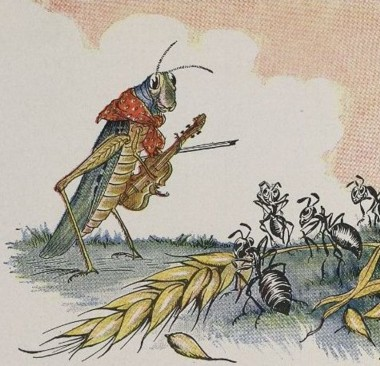
\includegraphics[width=1\textwidth]{ant-grashopper}  
	\caption[Ant and Grashopper]{Ant and Grasshopper, Illustration by Milo Winter from 1919 (1888-1956)}
	\begin{flushleft}
		\scriptsize{\citeauthor{Aesop}'s (\citeyear{Aesop} BC) ``Ant and the Grasshopper'', illustrated by Milo Winter (1888-1956) in 1919. Originally uploaded by \href{http://www.gutenberg.org/etext/19994}{Project Gutenberg}, via \href{http://commons.wikimedia.org/wiki/File:The-Ant-and-the-Grasshopper---Project-Gutenberg-etext-19994.jpg}{Wikimedia}}.
	\end{flushleft}
	\label{fig:ant-grashopper}
\end{figure}

It really is a fabled tax.

\subparagraph{History}
%last discussed, suggested in 2005 by Bush's tax reform group http://www.economist.com/node/5061687
%also get into the reasons why the USA tax failed.

\paragraph{Expenditure Tax (ET)} \phantomsection \label{sec:ET}
%must write this, it's simple
%I also think this is the evil twin!
%it is NOT cash-flow based!

%random ideas, edits, additions for thesis
%[ ] to bash FairTax.org (evil twins): http://www.taxpolicycenter.org/publications/urlprint.cfm?ID=901139
	%[ ] good source (popular) for the positional consumption race and its efficiency losses: http://prospect.org/cs/articles?article=postconsumer-prosperity#
	%[ ] really bash the Bradford X-Tax for good: It has limited progression (0-35% on the labor component, 25% on the non-labor VAT). This isn't exactly very good progression. Also, it falls only on labor. It's not a progressive consumption tax. It's a VAT with some poor relief.

\subsection{Taxes on Wealth} %substanzsteuer

\subsubsection{Taxes on Unimproved Nature}

%see diverse notes on google docs re: Dahrendorf krams

\paragraph{Land Value Tax (LVT)} \phantomsection \label{sec:LVT}
%needs to be written

%note about the LVT: it HAS limited income; it cannot be taxed beyond rental value people would simply stop using land at all (because the supply curve is completely inelastic).
	%so you might need other taxes, too. 
	%it's not clear how much value add comes from this one factor

%include the LVT in the circular flow diagram, together with other rents

%note that the LVT requires some difficult evaluations; it may cause some of the same illiqudity and other market reactions that we already now.
	%notably, market evaluations for untraded land (e.g. in the insurance business and/or for mortgages) will not help much, because these are in turn, market interactions that may be distorted, or equivalently, cause their own DWLs.
	%modern algorithms and data mining might help a little, in so far that land is comparable, which seems possible (it doesn't have sharp gradients).
	%alternatively, auctioning off land periodically might be the better solution to this problem -- it would have the same distributive effects (NO land rent), but may be politically difficult.
		%unclear if you can get the same steering effects on land concentration

%normative attractiveness: no one actually created land, it is but a by-product of capturing, or at one point, having captured, parts of land.

%there is a problem of transitional justice; people who have now invested in land, as opposed to other assets, may be at a disadvantage (or will they?)
	%if you have land, you're taxed on the unimproved value, if the rental value is lower, you don't use the land, so land use get's smaller, some land is abandoned (but it'll stop generating revenue at that point)
	%solow also says this: ‘Theoretical’’ is an essential qualifier here, because consensus evaporates once the papers turn to real-world implementation issues. One such issue is emphasized by discussant Robert Solow (p. 278): high tax rates on land values would mean departing dramatically from existing tax policy, with correspondingly dramatic capital losses: ‘‘Expropriating land values today would have no semblance of fairness. Suppose I have just paid through the nose for a prime beach lot. I have no unearned increment from the land. If you now tax away the rent, you are in effect taxing away the savings that enabled me to buy it. The original appropriator of the land is long gone.’’ /this is via \cite{Tomlinson2001}


%— Adam Smith , The Wealth of Nations, Book V, Chapter 2, Article I: Taxes upon the Rent of Houses:
	%Ground-rents are a still more proper subject of taxation than the rent of houses. A tax upon ground-rents would not raise the rents of houses. It would fall altogether upon the owner of the ground-rent, who acts always as a monopolist, and exacts the greatest rent which can be got for the use of his ground. More or less can be got for it according as the competitors happen to be richer or poorer, or can afford to gratify their fancy for a particular spot of ground at a greater or smaller expense. In every country the greatest number of rich competitors is in the capital, and it is there accordingly that the highest ground-rents are always to be found. As the wealth of those competitors would in no respect be increased by a tax upon ground-rents, they would not probably be disposed to pay more for the use of the ground. Whether the tax was to be advanced by the inhabitant, or by the owner of the ground, would be of little importance. The more the inhabitant was obliged to pay for the tax, the less he would incline to pay for the ground; so that the final payment of the tax would fall altogether upon the owner of the ground-rent.
	
%note neutrality of the tax

%Paul Samuelson: Paul Samuelson strongly supported a land value tax. "Our ideal society finds it essential to put a rent on land as a way of maximizing the total consumption available to the society. ...Pure land rent is in the nature of a 'surplus' which can be taxed heavily without distorting production incentives or efficiency. A land value tax can be called 'the useful tax on measured land surplus'." (wikipedia)

%Friedman from Wikipedia: Milton Friedman stated: "There's a sense in which all taxes are antagonistic to free enterprise -- and yet we need taxes. ...So the question is, which are the least bad taxes? In my opinion the least bad tax is the property tax on the unimproved value of land, the Henry George argument of many, many years ago."

%Krugman from Wikipedia: Paul Krugman agrees that a land value tax is efficient, however he disputes whether it should be considered a single tax, as he believes it would not be enough alone, excluding taxes on natural resource rents and other Georgistesque taxes, to fund a welfare state. "Believe it or not, urban economics models actually do suggest that Georgist taxation would be the right approach at least to finance city growth. But I would just say: I don’t think you can raise nearly enough money to run a modern welfare state by taxing land [only].” http://www.psmag.com/politics/this-land-is-your-land-3392/

%The Nobelist Joseph Stiglitz writes "Not only was Henry George correct that a tax on land is non-distortionary, but in an equilibrium society ... tax on land raises just enough revenue to finance the (optimally chosen) level of government expenditure.

%\cite{Tomlinson2001}
	%Book reviews / Regional Science and Urban Economics 31 ( 2001 ) 601 – 641 635
 %properties that sell are developed properties. Reschovsky’s concluding comment (p. 234) underscores the issue’s significance: ‘‘In my view, the most important unresolved issue concerning the adoption of a land value tax by a city or state government is the ability of that city or state to provide high-quality land value assessments that will be widely accepted by taxpayers, and will reflect as closely as possible the ‘highest and best use’ of each parcel of land. Experts clearly disagree about the feasibility of assessing land values. One way to resolve this issue would be for at least one state to attempt to implement a serious state-wide assessment of land values. This in turn would allow for full evaluation of the land value tax in a state or local government setting.’



\subparagraph{Pigouvian Element.} %comment on its pigouvian element, 

\subparagraph{Other Natural Resources}
%... but NOT CO2E, it does not replace that, it only deals with the inequality AND a little bit the commons problem of resources
%when applied to other material resources, too, the LVT becomes a, or might replace severance taxes.

%also compare this to auctioning off. The same could be done for land, except that would require land reform, so maybe the LVT is the smarter choice.

%notice that this unlikely to hit farmers (as they might expect) and other marginal uses of land.

%also notice the foundational beauty of this (smith mentions it): it's about taxing that part of your property that is valuable because of the stuff that other people around it (and public infrastructure) are doing. It's so beautiful.

\subsubsection{Taxes on Property}

\paragraph{Property Tax} \phantomsection \label{sec:PT}
%note use in the US for local school finance
%only on real estate, but could be other stuff

\paragraph{Stamp Duty} \phantomsection \label{sec:SD}

\subsubsection{Taxes on Net Worth}

\paragraph{Wealth Tax (WT)} \phantomsection \label{sec:WT} The Wealth Tax is a tax on the net wealth ($assets$ $-$ $liabilities$) of natural persons. It requires a balance sheet account for all tax liable individuals, including some method of valuation for \hyperref[des:NoIlliquidAssets]{illiquid assets}. Wealth Taxes are typically progressive in schedule. They are levied only in a few OECD countries, including France (up to 1.8\% p.a.) and Switzerland (up to 1.5\% p.a.).

%Include the estate and gift taxes as a subclass of taxes on net worth, because these are just triggered at a particular point in time (death). They are, crucial and by definition, not income taxes because they are not LINKED TO ANY EXCHANGE, for if they were, they would be incomes. Also note this in the definition of incomes: they are exchange incomes, not gifts.
	%or are they? maybe I need to include gift and estate taxes somewhere ...

%mention subsets Property Tax \gls{PT} and Stamp Duty \gls{WT} here. Also refer to \gls{LVT}

\subsection{Non-Taxes}

\paragraph{Financial Transaction Tax (FTT)} \phantomsection \label{sec:FTT}
%need to write this

\paragraph{Ecotax} \phantomsection \label{sec:Ecotax}
%need to write this
%note that this is not actually a tax in germany, but just a bunch of changes in different quantity taxes on energy.

\paragraph{Negative Income Tax (NIT)} \phantomsection \label{sec:NIT} The Negative Income Tax (NIT) is a subsidy for low wage earners, not a tax. It does not raise, but spends revenue. It is included here because of its broad redistributive impact and its technical implementation as a ``tax''. 

The NIT was suggested by Milton \cite{Friedman1962} as an elegant replacement for minimum wage legislation and \hyperref[sec:StructuralUnemployment]{broadly equivalent} (page \pageref{sec:StructuralUnemployment}) social security transfers. Under the NIT, workers would receive progressive transfer payments for hourly market wages below the socially acceptable minimum. However, in contrast to current income supplements, real market wage increases are not entirely eaten up by transfer cuts: at any given level of income, earning more on the market will leave you with more net in the bank. For example, under a minimum acceptable hourly income of \euro{}7.50 (current minimum wage proposal in Germany), moving from a \euro{}2.00 market price to a \euro{}4.00 market price job could increase your post-tax income from \euro{}7.50 (transfer \euro{}5.50) to \euro{}8.50 (transfer \euro{}4.50), always maintaining your incentives to earn more on the market. This may also help to counteract rent-seeking exploitation by low-paying firms.

\section{The Contest} \label{sec:contest} I now compare the merits of the above taxes according to the desiderata established so far. It will not be necessary to score every individual tax. Instead, they can be grouped in families of taxes all performing roughly equivalently in terms of the desiderata relevant here.

Results are summarized in \autoref{sec:Scores}.

May the perfect tax win.

\subsection[Indirect, Proportional Taxes]{The Forerunner ---\\Indirect, Proportional Taxes: VAT \& Payroll} \label{sec:ScoreVAT} Indirect, proportional taxes are the forerunners in tax choice today. For the last two to three decades, they have assumed an ever greater share of GDP, compared to other taxes (for Germany and the UK, see \citealt{Kemmerling2009}: 11). 

VAT and Payroll, for all their differences, share key characteristics: they are indirect, they are proportional and they fall on relatively immobile bases.  %and therefore, Payroll, at least, is regressive

\paragraph{Neutrality.} The key merit of indirect, proportional taxation is its neutrality to relative prices in the economy: deadweight losses are indeed \hyperref[des:DWL]{minimal}, as per desideratum \ref{des:DWL}. 

\subparagraph{Everyone Has to Consume.} For the VAT, the neutrality case is clear-cut. Ultimately, people can only spend the savings and (capital, labor) income they have on goods on the market. If buying of \emph{all} goods is proportionally taxed, people have no way to avoid the tax. They \emph{cannot} react to a price signal that is \emph{universally} increased: their \hyperref[eq:PED]{price elasticity of demand} (page \pageref{eq:PED}) is minimal. The same holds for sellers: they have to sell to someone. When every potential buyer has to bear the same tax, sellers have no way to react. Their \hyperref[eq:PES]{price elasticity of supply} (p.~\pageref{eq:PES}) is minimal, too. The VAT falls on a \hyperref[des:tax-inelastic]{maximally inelastic base} as per desideratum \ref{des:tax-inelastic}. 

\subparagraph{Everyone Has to Work \ldots} A proportional payroll tax is neutral when one accepts an exclusive, \hyperref[sec:OSN]{ordinary savings norm} (page \pageref{sec:OSN}). When capital rents are only \emph{compensation} for risky, deferred consumption all savings and capital rents are ultimately labor incomes. Under the \hyperref[sec:OSN]{ordinary savings norm}, someone living off her savings is someone living off her past work. In short, to consume and to live at all, everybody has to work, for someone, sometime. If you have to work for someone, and every potential employment is subject to the same, proportional tax, you cannot react to the tax. Again, the \hyperref[eq:PES]{price elasticity} of labor supply (page \pageref{eq:PES}) is minimal. The same holds for employers: they have to employ someone. If every potential employer is subjected to the same, proportional tax, their \hyperref[eq:PES]{price elasticity} of labor demand (page \pageref{eq:PES}) is minimal, too\footnote{In the real world, payroll taxes are levied only on employees, and not on self-employed people. That practice \emph{does} change relative prices of employed and self-employed work. Analytically, this discrimination is an aberration from a perfect payroll tax. In principle, self-employed people should be liable for a payroll tax on the wages they pay themselves.}.
	%scheinselbständige shows how this loophole can be exploited - often to the detriment of the self employed person.

\subparagraph{\ldots Except the Rich.} Under a \hyperref[sec:Y2C]{yield to capital norm} (page \pageref{sec:Y2C}), a proportional tax is not neutral. When capital rents are a genuine increment to wealth, there is an alternative to work: you can either work, or live off your interest. In formal terms, rich people can substitute their labor income with capital income. As the availability of substitutes increases price elasticity, the labor supply by rich people is no longer price inelastic. Absent the payroll tax, they might have elected to work more than they will if their labor income is taxed. 
	%this is, at the and, questionable. Do people really work more because of pay? at which level? discuss homo econ. Resolution: if incentives should matter, to the degree that they do, we should maie it netraul. If they are, as I suspect, neglibible/strictly limited, corrects should be small.

\subparagraph{Ideally, A Ordoliberally Hygienic Tax.} A neutral tax, by definition, has no fee or pigouvian component. A VAT or payroll tax with a proportional, uniform rate is \hyperref[des:OrdoliberalHygiene]{ordoliberally hygienic} as per desideratum \ref{des:OrdoliberalHygiene}. 

\paragraph{Redistribution $=$ General Revenue?} To the extent that proportional taxation is accepted as an equity norm (!), a VAT or payroll that goes into general government revenue is a proper instrument both to \hyperref[des:RedistributionAndRevenueAreOne]{redistribute and to raise revenue}, as a desirable tax should as per desideratum \ref{des:RedistributionAndRevenueAreOne}. 

In Germany and many other countries, \emph{capped} payroll taxes are used to raise social insurance contributions. Here, redistribution and revenue generation undesirably interact. 

First, \hyperref[sec:SICAreTaxes]{social insurance contributions are proper taxes} (page \pageref{sec:SICAreTaxes}): they serve to pool risks and they redistribute between old and young, healthy and sick. Second, these services are actually provided universally and unconditionally: as a last resort, the (German) welfare state pays even for those who have \emph{not} contributed. The welfare state polity, has in other words, already adopted an allocative norm.

Raising revenue for these very services on a \emph{regressive} schedule (capped) on only some incomes (employed labor) embodies another, very specific allocation, for which no normative justification is readily available. In Germany, only employed people pay for the health insurance of all other employed people. Exactly \emph{why}, at minimum, self-employed people do not also contribute to this risk pool is unexplained, but allocatively consequential.

\paragraph{Fairness.} At best, a VAT or payroll tax can be regarded as a proportional taxation on \hyperref[des:PersonalTaxation]{natural persons} as per desideratum \ref{des:PersonalTaxation}\footnote{
	Social insurance contributions as a selective payroll tax on capped labor incomes \emph{do not} fall on all natural persons, but only some. Again, an ideal payroll tax would burden everyone.}. 
It cannot accommodate \hyperref[des:Progression]{progression}, let alone an \hyperref[des:SharpProgression]{arbitrarily steep schedule} as per  desiderata \ref{des:Progression} and \ref{des:SharpProgression}. 

\subparagraph{Payroll: Regressive.} An (ideal) payroll tax is proportional only under an \hyperref[sec:OSN]{ordinary savings norm} (page \pageref{sec:OSN}). When capital rents are regarded as proper income (\hyperref[sec:Y2C]{Yield-to-Capital Norm}, page \pageref{sec:Y2C}), a payroll tax falls only on one of two types of incomes. A payroll tax is clearly not \hyperref[des:StructuralAgnosticism]{agnostic towards labor and capital incomes}, as mandated by desideratum \ref{des:StructuralAgnosticism}. 

\subparagraph{VAT: Proportional.} No matter the savings norm, a VAT is straightforwardly proportional, because \emph{all} income is ultimately consumed and tax liable to generate utility. 
	%include argument, table, example here

\subparagraph{Different Rates Are Not An Option.} One common alteration to make the VAT fairer is to adopt different rates for different types of products. Goods that cover basic needs (food) often enjoy a lower VAT rate. In a complex economy and modern society, it is impossible to easily determine which goods satisfy basic needs and which do not. Is a meat a basic need? Is a filet mignon? Is a filet mignon every day?
%more generally, this violates the norm of neutrality, it will affect less people who buy 10 sedans than people who buy 1 luxury car. This is about as non-agnostic as it gets.

When the state \emph{does} establish different VAT rates, it risks becoming a micro-manager of fairness and will create arbitrary incentives for cross-substitution.
	%&also, there are loopholes for fraud!

\paragraph{The Problems of Proportional Taxation.} Aside from not being progressive, a proportional tax raises a number of \hyperref[sec:Efficiency]{efficiency} problems (page \pageref{sec:Efficiency}). 

\subparagraph{Diminishing Utility and Positional Consumption.} As proportional taxes, VAT and payroll cannot consider \hyperref[des:DiminishingUtility]{diminishing marginal utility} of wealth, income or consumption as demanded by desideratum \ref{des:DiminishingUtility}. Whether you are struggling to pay for the first class trip of your child or whether you are thinking about signing up your child for the third summer school, the taxman will treat these two transactions equally, irrespective of the clearly differential impact on the subjective well-being --- not to mention opportunity --- of parents and child in these two families. 

Similarly, a proportional VAT on consumption can also not \hyperref[des:ConspicuousConsumption]{curb positional consumption} as mandated in desideratum \ref{des:ConspicuousConsumption}. Whether you are buying a high-priced Mercedes sedan because you enjoy a luxury car during your frequent trips on the German autobahn, or whether you are buying it merely because you do not want the smaller car than your neighbor, the taxman will treat these two transactions equally, with no regard to a potentially wasteful, positional component of consumption.

\subparagraph{Proportional Taxation Raises the Effective Price Floor of Labor.} \phantomsection \label{sec:PropTaxDWL} Most problematically, any proportional taxation will make it relatively more expensive for low-income earners to make ends meet. In welfare states with legislated or effective minimal standards of living, such an increase in the real costs of living will push more people into structural unemployment. When every trip to the grocery store gets more expensive, more low-skilled people will be unable to afford a socially acceptable minimal standard of living from their equilibrium incomes. Conversely, the (very price-elastic) demand for such low-qualification service jobs drops dramatically, as struggling workers try to extract higher wages (Scharpf in foreword to \citealt{Ganghof2004}: 12ff). An equivalent dynamic holds for proportional payroll taxes.

Proportional taxation raises the \hyperref[des:LowPriceFloor]{effective price floor for low-productivity labor} in violation of desideratum \ref{des:LowPriceFloor}. Present some income-replacing transfer scheme, as is nearly universally the case in developed welfare states, supply for low-productivity work becomes very elastic: you can either work for \emph{less} net purchasing power, or receive \emph{same} or a little more from the state for not working at all. Proportional VAT or payroll taxation then creates a substantial \hyperref[des:DWL]{DWL} of structural unemployment, disallowed in desideratum \ref{des:DWL}\footnote{
	This is \emph{not} some kind of welfare-mother argument. It is not that lazy people cause structural unemployment and free-ride on the polity. Rather, the polity makes it systematically impossible for some of its members to participate gainfully in the economy.}.
		%gainfully and dethly?
		%add a neoliberal source that argues for natural unemployment here.

\subparagraph{Limited Stabilization.} Proportional taxation, by definition cannot serve as an \hyperref[des:AutomaticStabilizer]{automatic stabilizer}, as demanded by desideratum \ref{des:AutomaticStabilizer}. When the schedule is linear, it does not matter how lumpy your consumption is. A VAT or ideal payroll will do nothing to prevent you from buying nothing during a bust, and too much during a boom. 

A proportional VAT could, theoretically serve as an \hyperref[des:DiscretionaryStabilizer]{discretionary stabilizer} if government were to lower the VAT rate during the downturn. People would have an incentive to buy at lower taxes during the downturn, rather than later at higher rates.

Unemployment insurance works as an automatic stabilizer because of how the revenue is \emph{used}, and not how it is \emph{raised}. Consumption is smoothed out as the incomes of laid-off workers are insured in the medium term. Two problems remain: First, laid-off workers can still consume less than they optimally should, maybe because they are anticipating a prolonged, uninsured downturn. Second, unemployment insurance would be a much better automatic stabilizer if it were raised in a manner that also smoothes consumption. 

\paragraph{A Mixed Bag For Capitalism.} On the pro side, a VAT and proportional payroll tax let \hyperref[des:Entrepreneurship]{entrepreneurs make their own production decisions}, and on their own \hyperref[des:Incentives]{dime and incentive}, as mandated in desiderata \ref{des:Entrepreneurship} and \ref{des:Incentives}.

A VAT and proportional payroll tax also do not require \hyperref[des:NoIlliquidAssets]{evaluation of illiquid assets}, as disallowed by desideratum \ref{des:NoIlliquidAssets}.

On the other hand, a VAT and proportional payroll tax does little to avoid \hyperref[sec:GovDynofIneq]{runaway capital accumulation} (page \pageref{sec:GovDynofIneq}ff.). If capital is concentrated in the hands of only a few people, the rest will not be \hyperref[des:BroadOwnership]{able to close intelligently incentivized deals} on their unobservable effort and uncertain innovations. Tightly concentrated capital is in violation of desideratum \ref{des:BroadOwnership}.

\paragraph{A Tiny Little Bit Difference Principle.} For all its equity and efficiency shortcomings, a proportional VAT shares the fundamental merit of all consumption taxes: it taxes a normatively justifiable basis. Taxing consumption, not incomes, may be desirable under the the \hyperref[des:DifferencePrinciple]{difference principle}, as per desideratum \ref{des:DifferencePrinciple}. This \hyperref[sec:FoundationalBeauty]{foundational argument} is presented in greater detail and strength in \ref{sec:FoundationalBeauty} on the \emph{Progressive} Consumption Tax. Absent progression, the difference principle merits of the VAT are negligible.

The merit of consumption taxation under VAT also manifests itself in the (somewhat\footnote{
	Only a PCT, by virtue of its progressive schedule, will \hyperref[sec:ScorePCT]{allow for a truly \emph{arbitrary} savings rate} as argued in \autoref{sec:ScorePCT}.}
\hyperref[des:Savings]{positive savings rate} it allows for, as mandated in desideratum \ref{des:Savings}. If government would raise its revenue exclusively through a VAT, people's incentive to save would be unaltered: as argued in the above, a VAT is agnostic towards capital or labor incomes. 

\subsection[Direct, Progressive Taxes]{The Old Hand ---\\Direct, Progressive Taxes: PIT, CIT \& Dual PIT} \label{sec:ScorePIT} The Personal Income Tax (PIT) is the archetypical modern tax designed to redistribute. It was conceived in the early to mid 19th century to address the inequities of early capitalism. 

\paragraph{Income Taxation Punishes Saving.} A PIT can cause two different kinds of \hyperref[des:DWL]{DWLs disallowed} in desideratum \ref{des:DWL}. 

First, if insufficiently progressive (= near proportional), it causes the \hyperref[sec:PropTaxDWL]{DWL of proportional taxation} discussed for VAT and payroll taxes (page \pageref{sec:PropTaxDWL}).

Second, if it is sufficiently progressive on both labor and capital incomes, it taxes savings twice: once when they are earned, and a second time when they yield an interest (and yet again when they yield a compound interest). This has a number of negative implications.

When people can avoid double taxation by consuming income right away, they may very well do so. Capital incomes are taxed, even though saving is elastic. This conflicts with desideratum \ref{des:tax-inelastic} (\hyperref[des:tax-inelastic]{tax inelastic bases}). Things become even more awry when we consider investments (savings) of different risk. When the (uncertain, but hiwher) rewards of risky investment are taxed progressively, people will have a smaller incentive to run the risk in the first place. The PIT still allows for \hyperref[des:entrepreneurship]{local, decentralized production decisions} as per desideratum \ref{des:entrepreneurship}, but \hyperref[des:incentives]{incentives} are substantially dampened in violation of desideratum \ref{des:incentives}. 

Because it taxes savings twice, a PIT is in violation of desideratum \ref{des:Savings} on an \hyperref[des:Savings]{arbitrary savings rate} (page \pageref{des:Savings}) and desideratum \ref{des:StructuralAgnosticism} on \hyperref[des:StructuralAgnosticism]{structural agnosticism} (page \pageref{des:StructuralAgnosticism}). A PIT discourages saving, and it falls twice on capital income, and only once on labor income.
	%simplyfy language
	%also: use income-source agnosticism instead of the other term?

\paragraph{The Merits of Progression.} To the extent that a PIT is progressive, it satisfies desiderata \ref{des:DiminishingUtility} on \hyperref[des:DiminishingUtility]{the diminishing marginal utility of income} (page \pageref{des:DiminishingUtility}) and \ref{des:Progression} on \hyperref[des:Progression]{progression} (page \pageref{des:Progression}). It also serves to \hyperref[des:LowPriceFloor]{lower the price floor} of labor as per desideratum \ref{des:LowPriceFloor}. The problematic double taxation of capital incomes also serves to substantially dampen \hyperref[sec:GovDynofIneq]{runaway capital accumulation} and ensures \emph{some} degree of \hyperref[des:BroadOwnership]{broad ownership} as mandated in desideratum \ref{des:BroadOwnership} (\citealt{McCaffery2005}: 810). 
	%degree of ownershiop depends on the spending side, too, of course. Explain this

\paragraph{The Limits of Progression Under the PIT.} A tax on \emph{income}, by definition, does little to \hyperref[des:ConspicuousConsumption]{curb positional consumption} as mandated in desideratum \ref{des:ConspicuousConsumption}. 

More fundamentally, a PIT does \emph{not} allow for truly \hyperref[des:SharpProgression]{arbitrarily steep schedule} as per desideratum \ref{des:SharpProgression}. For a high \emph{average} tax rate on incomes say, 50\%, \emph{marginal} tax rates would be prohibitively high. Such high marginal tax rates would all but destroy \hyperref[des:Incentives]{incentives to invest} at that margin at all, violating desiderata \ref{des:Incentives}, \ref{des:Savings}, \ref{des:DWL} and \ref{des:tax-inelastic}. It seems likely that a PIT will be no match to the \hyperref[sec:GovDynofIneq]{governing dynamics of self-reinforcing inequality} (page \pageref{sec:GovDynofIneq}), given its limited steepness in progression.
	%again, via coinsumption, it also applies to the PCT: Or it doesnt because compount interest?

\paragraph{No Stabilization.} As any tax on income, the PIT cannot serve as an effective \hyperref[des:AutomaticStabilizer]{automatic stabilizer}, or \hyperref[des:DiscretionaryStabilizer]{discretionary stabilizer} as demanded in desiderata \ref{des:AutomaticStabilizer} and \ref{des:DiscretionaryStabilizer}.

\paragraph{The Systemic Flaws of the PIT.} Aside from its limited and problematic merits, the PIT carries with it some unavoidable, inherent flaws.

\subparagraph{The PIT's Ugly or Unfair trade-off: Accrual vs. Realization.} Because the PIT is based on flows of economic welfare, it requires a method to measure these flows. Whenever assets are \hyperref[sec:Illiquid]{illiquid} (page \pageref{sec:Illiquid}), the taxman can either wait indefinetely for realization, or tax on some assumed accrual. Either way, substantial welfare losses ensue and desideratum \ref{des:NoIlliquidAssets} on the \hyperref[des:NoIlliquidAssets]{minimal taxation of illiquid assets} is violated.
	%pct requires balance sheet accounting! not just cash-flow!

Income taxation on accrual or realization also has substantial equity implications. In contrast to the VAT, it is \emph{not} merely a matter of timing when we pay the income tax. 

\begin{quote}
	``Such a statement reveals a basic failure to understand --- or a desire that others not understand --- the nature of income taxation and tax avoidance: [\ldots] if income tax can be postponed [\ldots], interest (or other capital income) can be earned on a tax deferred basis in the meantime.'' (McLure 1988 as cited in \citealt{Seidman1997}: 125).
\end{quote}
	%twitter this!

In short: taxation on realization ignores compound interest.

\subparagraph{Tax Evasion 101: Buy, Borrow, Die.} \phantomsection \label{sec:TaxEvasion101} A sinister exploitation of the evaluation problem of the PIT goes by the name of \emph{buy, borrow, die}\footnote{
	I take these lessons in ``tax planning 101'' --- only slightly tongue in cheek --- from \citeauthor{McCaffery2005}'s seminal piece on \emph{A New Understanding of Tax} (\citeyear{McCaffery2005}: 888ff).}. 
It emerges from the following three doctrines, all of which make sense in isolation.

%McCaffery:
	%taxes have become voluntary.Read more at location 57   • Delete this highlight
	%Add a note


First, a PIT never taxes debt as income. It makes little sense to tax debt: according to \citeauthor{Haig1921}-\citeauthor{Simons1938} (equation {eq:HaigSimons}) and common intuition, the income-generating ability of a person does not change just because she takes out a loan. Consequently, people pay their taxes on the income they use to repay principal and interest.

Second, for the practical reason of avoiding evaluations by a central planner, the PIT is levied on realization, not accrual.

Third, for \citeauthor{Haig1921}-\citeauthor{Simons1938} and common intuition, heirs are (estate) taxed only net of assets and liabilities handed down to them. 

So far so good? These three trivially intuitive doctrines, in combination constitute the fatal achilles heel of effective capital income taxation. Tax evaders can follow a simple, and entirely legal strategy. First, they \emph{buy} appreciating, but illiquid assets. In a second step, they \emph{borrow} money on the appreciating asset as collateral. Recall that this cash inflow is not taxed. Also recall that lenders may very well consider the yet-illiquid appreciation of the asset in extending their loan terms. Tax evaders can now spend out of the appreciation of the asset without paying \emph{any} capital income tax on this de-facto accrual of welfare. Third, tax evaders \emph{die} and bequest their assets to someone else. That someone else is liable only for estate tax on the \emph{net} value of the assets and liabilities. The consumption of the deceased tax evader is deducted from the net value. Again, ultimately, and irrevocably, consumed capital incomes escape taxation.
	%alternatively, you make inheritors liable for the decades of tax liability and they'll just pass on the inheritance

This loophole, like the underlying problem of \hyperref[sec:TaxIlliquid]{illiquid assets}, is \emph{not} a practical aberration that could conceivably be closed. Any income tax on realization will offer this evasive strategy. 
%is this an entirely new problem, or does this fall adequately under "don't tax illiquid stuff?" Can I break it down like that? Or is there maybe another thing behind it? Timing? Is it all accrual vs realization?

This is not a hypothetical or esoteric problem. The pre-2007 housing bubble in the U.S., Spain and elsewhere was --- amongst other factors --- also fueled by this strategy. Houses were good illiquid assets (\emph{buy}). Banks willingly offered mortgages on the houses (\emph{borrow}). They also happily refinanced the loan, if the suggested (but unrealized!) fair market value of the house had increased. Consumers took out a bigger mortgage on the (supposedly) appreciated house and spent the difference on a new SUV and a flat screen TV. All tax free.

Appreciation in illiquid assets is no small component of our economic growth. A colossal share of the real welfare that accrues to capital income earners escapes income taxation without further notice, and any readily available fix.

\subparagraph{The PIT's Ugly Backstops: The Estate and Gift Tax.} It follows from the strategy of tax evasion 101 that an estate and gift tax are necessary backstops to the PIT. Without a tax on the substance bequested, unrealized appreciations on illiquid assets would go entirely untaxed. With an estate and gift tax, ``only'' the consumed part of unrealized appreciations escapes taxation.
%Note: the "pure income tax" maybe a cat-dog (Sartori 1991: 247). It's not an actual category.

The estate and gift taxes are, in themselves ugly beasts. Just like the PIT, they require an evaluation of a flow of economic welfare in the potential absence of a market equilibrium price of that very flow. If an entrepreneur bequests her family-owned firm to her daughter, no one can know how much it is worth. Again, problems in the \hyperref[sec:Illiquid]{taxation of illiquid assets} ensue (page \pageref{sec:Illiquid}). 

\subparagraph{The PIT's Ugly Backstops: The CIT.} \phantomsection \label{sec:ScoreCIT} A PIT has another, even uglier backstop: the Corporate Income Tax. Recall that a PIT is meant to tax all incomes, including interest and compound interest. With only a PIT, tax evaders would have at their disposal a strategy even simpler than tax evasion 101: they could place (or retain) their savings in an incorporated firm. First, tax evaders could spread out their (spiky) income over a longer period of time to play the progressive schedule. A small, but steady trickle of income is better than a large, lumpy flow under a progressive tax. Second, and more fundamentally problematic, tax evaders can also retain their initial capital income in the corporation and have it earn a compound interest. Note that the compound interest is earned on a capital income which, ideally, \emph{should} have been taxed \emph{already}.

To avoid this loophole, a PIT needs a CIT to get at the corporate shelter from the income tax (\citealt{Genschel2005}: 7). Also empirically, PIT and CIT rates go hand in hand, between countries and over time, further supporting the intricate, if dysfunctional link between the two (\citealt{Piatkowski2008}: 14).

The CIT is as bad as the PIT, minus the merits of progressive, personal taxation of the PIT.

First, the CIT has no \hyperref[des:TaxIncidence]{well-determined incidence} as demanded in desideratum \ref{des:TaxIncidence} (\citealt{McCaffery2005}: 918). Corporations are fictions. If you tax them anyway, you violate desideratum \ref{des:PersonalTaxation} (\hyperref[des:PersonalTaxation]{personal taxation}). 

Second and related, the CIT knows no progression. To the extent the the CIT ever reliably fell on capital, it made some sense historically when corporate ownership was a reasonable proxy for the propertied classes. This is no longer the case. Many people receive capital incomes (\citealt{Grabka2007a}: XV). The CIT has no way of distinguishing \emph{between} different owners (\citealt{McCaffery2005}: 918). Whether a particular Volkswagen share belongs to the life insurance of a single working mother or a stock market tycoon, both are taxed at some uniform corporate income rate . %the CIT is also not internally progressive.

Third, much like the PIT, the CIT itself is plagued by unavoidable loopholes. The CIT is very sensitive to international tax rate competition: if CIT rates differ from country to country, multinational companies can easily shift profits to the country with the lowest rate. A number of strategies are available to do this, the simplest of which is to charge inflated (deflated) prices in intra-company trade (\citealt{Ganghof2004}: 43ff). 
	%this, in fairness, applies to all prigressive taxes
This loophole cannot be closed as inflation (deflation) of intra-company trade prices cannot be reliably detected. More fundamentally, ``any national claim to a particular share of [a multinational's] profits is hard to justify on the basis of principle`` (\citealt{Genschel2005}: 61). %also explain how they can always calculate themselves to zero, not just with arbitrage.

\paragraph{The Downgraded Upgrade: The Dual PIT.} \phantomsection \label{sec:ScoreDualPIT} To the extent that a Dual PIT has substantially lower, and proportional rates on capital incomes, it alleviates the PIT's disincentives to \hyperref[des:Savings]{save} and \hyperref[des:Incentives]{invest} as per desideratum \ref{des:Savings} and \ref{des:Incentives}. The Dual PIT is simply another non-\hyperref[des:StructuralAgnosticism]{agnostic} relative burdening of capital and labor incomes in violation of desideratum \ref{des:StructuralAgnosticism}. 

\subparagraph{A Hollowed-Out PIT.} The relatively smaller burden on capital is hard to justify on principle. The largest incomes are, by definition, capital incomes\footnote{
	Recall that to have a capital income one first has to have a surplus of unconsumed labor income.}. 
Charging capital incomes a lower, proportional rate will greatly depress the overall \hyperref[des:Progression]{progression} of the PIT, in violation of desideratum \ref{des:Progression}. Progression is limited under the PIT already, but will be even more compressed under a dual rate structure, in violation of \ref{des:SharpProgression}.

To the extent that more of the tax burden falls on labor, a Dual PIT will also raise the \hyperref[des:LowPriceFloor]{price floor for low-productivity labor supply}, as disallowed in desideratum \ref{des:LowPriceFloor}. 

The Dual PIT is a PIT only in name. It hollows out the ideal of universal progression. %universal progression is an ideal, why? 
The lower the rate on capital gets, the more a Dual PIT approximates a (progressive) payroll tax.

\subsection[Business Tax]{The Streaker ---\\Local Business Tax (LBT)} \label{sec:ScoreLBT} A tax on the earnings of local businesses shares all of the disadvantages of the CIT.
	%is the idiom clear enough? add picture of a litzer
	%also include the financial transaction tax here

More fundamentally, the LBT is not a proper tax. It should not need to be discussed here at all. 

Local authorities provide different kinds of \hyperref[tab:types-of-goods]{goods} (see \autoref{tab:types-of-goods}). The \hyperref[sec:Redistribution]{redistribution}, \hyperref[sec:RiskPooling]{risk pools} and \hyperref[sec:PublicGood]{public goods} it provides should be financed out of \hyperref[tab:TaxResponses]{general revenue}, as outlined in \autoref{tab:TaxResponses}. A general revenue tax should fall only on \hyperref[des:PersonalTaxation]{natural persons} as per desideratum \ref{des:PersonalTaxation}. 

Local authorities also provide \hyperref[sec:CommonGood]{common goods} such as parks and \hyperref[sec:NaturalMonopolies]{natural monopolies} such as sewers \footnote{Sometimes, at the margin of local decisions public goods also become common goods or natural monopolies: that extra motorway feeder may be necessary only for a small number of logistically intensive firms (rival consumption) and local government may well negotiate with the interested firms on whether to build the road or not (exclusion).}. Common good and natural monopolies should be financed out of Pigouvian levies (at marginal cost) and fees (at average cost), respectively as per \autoref{tab:TaxResponses}.

The LBT sits in the nomansland somewhere between general revenue taxation and Pigouvian levy or fee. It violates the norm of \hyperref[des:OrdoliberalHygiene]{ordoliberal hygiene} as per desideratum \ref{des:OrdoliberalHygiene}.

To the extent that the LBT is used to finances risk pools, public goods and redistributes, it should not be allowed to differ between municipalities. If universal education is an allocative goal of the broader, national polity, everyone should pay for it. If fire protection is a public good, everyone should pay for it. LBT revenue used to finance these things should be replaced by transfers from higher levels of government. %to avoid arbitrage
	%reference fiscal federalism

To the extent that the LBT is used to finance common goods or natural monopolies, it must specifically fall (at marginal or average cost, respectively) on the very consumption of these goods, and not on the earnings of a firm in general. If industry pollutes a local river, \emph{every unit of discharged pollution} should be (Pigouvian) taxed at marginal cost, not every firm in the city based on their earnings. If some firms or citizens in a rural municipality require high-speed internet access (a natural monopoly), each \emph{user} of the network should pay at average costs, not every firm in the vicinity. %add: sometimes, such break-downs might be impractical, in that case, paying it out of general revenue might just be the better ticket. Also note that LVT can replace this purpose to some extent.

In short, the LBT is an anti-ordoliberal streaker that should never have entered this game of perfect taxation. It should be marshaled off the playing field as soon as possible.

\subsection{Impotent Redistribution}

\begin{quote}
	\emph{``Advocates of redistributive taxes must wake up and realize that their end is in jeopardy on account of their poor choice of means: they are fighting, and losing, the wrong war.''}\\*
	--- Edward J. McCaffery (2005: 848)
\end{quote}


\subsection[Progressive Consumption Tax]{The Dark Horse: Progressive Consumption Tax (PCT)} \label{sec:ScorePCT} 

%   * step back carefully from my assumptions: even if you don't agree with the politics (redistributive and axiomatic in terms of positional spending) of the pct, you've gotta agree with the efficiency.
%   * even if you don't agree with the PCT, you've gotta agree with the questions it poses.

%add a chapter on the failed USA tax, and the charge that it was too complex.

%Note that what Ganghof + Scharpf 2004: 37 is incorrect in their treatment of capital incomes. They are actually taxed, when they are consumed, given that the tax is cash-flow based (dissavings count!). Consider the Haig-Simons.
	%This is a widespread misunderstanding of the PCT, particularly with regards to its evil twins.
	%Contact Ganghof + Scharpf about this mistake!

% Fundamental agreement on the likely advantages of a PCT regime has been reached in the (albeit heterodox) economics literature (conceptually Brümmerhoff 1990: 357ff, empirically Tomer et al. 2008, normatively McCaffery 2002).

%What Is The Perfect Tax?
%Friedman is actually a fan of the PCT, and has argued to use it to pay for the war effort in the past. This is via Robert Frank 2011 (Darwin).

\paragraph{It's Win-Win-Win-Win: No DWL Or No DWL \& Less Waste Or Diminishing Marginal Utility.} \phantomsection \label{sec:WinWin} The DWL case for the PCT is not clear, but either way, it's good. 

Just in \emph{which} way the PCT is good depends on the \hyperref[eq:PED]{price elasticity of demand} in excessive and positional consumption. 
	%simplify the language

%let's be honest about this, the DWL case of a PCT is not so clear-cut. It might still disincentivize people, because at the end of the day, they get to enjoy less, although, only to the extent that there is actually no race. Also, note, that the PCT still does not tax compound interest.
%from \cite{ZimmFina2009}
	%   * Read p.  138-159
	%   * feature the Economic cycle page 139 in my thesis, argue why it makes more sense to tax consumption
	%   * 156: "Überschreitet die [Einkommens]Besteuerung jedoch ein gewisses Ausmaß, so ist zu erwarten, dass sich negative Auswirkungen auf Investitions- und Arbeitsbereitschaft ergeben und damit das Wachstum beeinträchtig wird. Dagegen könnte eingewandt werden, dass ein höherer Anteil der Einkommenssteuer bei gleichem Gesamtsteueraufkommen die Gesamtbelastung nicht verändert, sonder nur wahrnehmbarer macht, weil die Einkommenssteuer für die Besteuerten merklicher ist als die Verbrauchssteuer. Für die Wirkung auf Investition und Arbeitsbereitschaft ist aber wahrscheinlich nicht die tatsächliche Belastung eines privaten Haushalts oder Unternehmens entscheidend, sondern nur der Teil der Belastung, der wahrgenommen wird und in die ökonomischen Entscheidungen eingeht."
	%      * Bingo. This is the argument for the PCT vs PIT in terms of incentives.

%\cite{MusgPubl1976}
	%   * the PCT "is still a new and exciting idea" (315)
	%   * "In some respects, the approach would be simpler than under the income tax. The dilemma of how to deal with unrealized capital gains would disappear. If assets were sold, the proceeds would enter into the tax base unless offset by purchases of other assets or an increase in balances. Also, there would be no need to determine corporate profits. Dividends would appear as receipts and unrealized capital gains obtained through retention of profits or otherwise would be irrelevant until realization occurred and the proceeds were channeled into consumption. The difficult problem of depreciation accounting, similarly, would disappear." (316)
	   %   * bingo, bingo, bingo
	%   * "(...) distributional objectives might be achieved with less disincentive effects" (317)
	%   * Contras, needed (316)
	%      * complete recording of cash balances (OK)
	%      * inclusion of imputed consumption (homegrown foods, housing) (OK)
	%      * Borrowing must be acccounted for (indeed, OK)
	%         * "Where the lender was an individual, also subject to tax, he would see to it that this was done so as to reduce his own base; but where lending was by institutions not subject to the expenditure tax, lenders would have to be required to file information returns on loans made" (316)
	%         * (OK, this can be done by simply legislating that loans without such reporting are gifts.
	%      * consumer durables (OK)
	%      * "The expense-account problem, difficult enough under the income tax, would assume large proportions" (fringe benefits, acknowlegded)
	%      * education "would pose a similar problem, as they again involve both consumption and investment aspects" (OK)
	%   * "on balance, the administrative diffculties for an expenditure tax may well equal or outweigh those of an income tax. For higher-income individuals at least, more or less complete balance-sheet accounting would be needed. Yet, this is precisely the income range over which effective administration would matter most. At low levels of income, there is relatively little difference between an income and an expenditure tax approach. The distinctuon becomes of major importance only as we move up the income scale and the savings rate rises" (317)
	%      * yes, yes, yes, but I don't agree that you need balance-sheet accounting. Cash-flow suffices. %or do you? Actually you need balance-sheet accounting either way for personal progression.

Without further empirical research, they cannot be known. The PCT will have \emph{very} high marginal rates, possibly well above 100 \%. Because universal, stark price hikes in the markets for excessive consumption have never occurred, we have no systematic observations regarding the responsiveness of excessive buyers to such price changes. 

So what are the alternative outcomes?

\subparagraph{What If: People Still Consume Excessively.} If people \emph{do not} respond to the post-tax price hike in excessive consumption, the PCT will tax an \hyperref[des:tax-inelastic]{inelastic base}. The DWL will be \hyperref[des:DWL]{minimal}, as per desiderata \ref{des:tax-inelastic} and \ref{des:DWL}. Most of what consumers no longer enjoy in excessive consumption will be recouped as government revenue, as illustrated in \autoref{fig:DifferentIncidence}. 

Producers will be perfectly elastic in their supply. At least in the long run\footnote{This of course depends on a very gentle phasing in of the tax so as to allow producers to cheaply exit their production of excessive consumer goods, and cheaply enter another market. This requirement for the \hyperref[sec:Implementation]{implementation} of the PCT is further discussed in \autoref{sec:Implementation}.}, all producers can shift their production to less expensive consumer goods, or, as described later, to investment goods. The burden of the PCT will fall exclusively the \hyperref[des:PersonalTaxation]{natural persons} who ultimately consume goods, as mandated in desideratum \ref{des:PersonalTaxation}.

\subparagraph{What If: People Consume Less (Expensive) Things.} If people \emph{do} respond to the post-tax price hike in excessive consumption, the PCT gains a Pigouvian component, but one that works. When people consume excessively, they pay for the negative externality of defection in the \hyperref[tab:PositionalPD]{Prisoner's Dilemma of positional consumption} (page \pageref{tab:PositionalPD}). Recall that when the Joneses buy a BMW (defect) instead of a VW (cooperation), the utility enjoyed by the VW-owning Does decreases: they cannot stand having the cheaper car. Under the PCT, the Joneses pay (dearly) for showing off their BMW. If their demand for BMWs is price elastic, they may buy the same VW as the Does.

%\begin{table}
%		\caption{The Battle of the Sexes}
%		\label{tab:BoS}
%		\begin{center}
%		\begin{tabular}{m{1cm}m{2,3cm}m{2,3cm}m{2,3cm}m{2,3cm}}
%			& & \multicolumn{2}{c}{\emph{Man}} \\
%			& &Opera & Football\\ 
%			\cline{3-4}
%			\multicolumn{1}{c}{\multirow{4}{*}{\emph{Women}}} & \multirow{2}{2,3cm}{Opera} & 		\multicolumn{1}{|r|}{2} & \multicolumn{1}{r|}{0}\\ 
%			\multicolumn{1}{c}{} & \multicolumn{1}{c}{}& \multicolumn{1}{|l|}{3} & \multicolumn{1}{l|}{0}\\ 
%			\cline{3-4}
%			\multicolumn{1}{c}{} & \multirow{2}{2,3cm}{Football} & \multicolumn{1}{|r|}{0} & \multicolumn{1}{r|}{3}\\ 
%			\multicolumn{1}{c}{} & \multicolumn{1}{c}{}& \multicolumn{1}{|l|}{0} & \multicolumn{1}{l|}{2}\\ 
%			\cline{3-4}
%		\end{tabular}
%		\end{center}
%		\scriptsize{The Joneses and the Does are peers, positional consumers and in the market for a new car. Payoffs are the net of cost of car ($VW=0$, $BMW=-5$) and status gain from driving the \emph{relatively} more expensive car ($+10$ for superior, $-10$ for inferior, else $0$). Larger payoffs are better.\\
%		Prices of the BMWs are inflated so as to include the societal costs of wasteful consumption, here, as in an ideal world, accruing only to the buyer.}
%	\end{table}
%why is this table still in here?

%positional consumption PD is now in mixed economy


Also recall that the level of cooperation in a multiplayer Prisoner's Dilemma is a \hyperref[sec:CommonGood]{common good} (page \pageref{sec:CommonGood}). Contributing to cooperative behavior creates a benefit to other players from which they cannot be \emph{excluded}. Establishing cooperation is, however, \emph{rival}: if no one, or too few people cooperate, the benefits of cooperation will not materialize. Buy buying a VW, the Does contribute to a common-good-like lower level of automobile consumption, from which everyone else can invariably (relatively) benefit. The Joneses can exploit the thriftiness of the Does by buying a BMW (greater relative utility), or they can partake in the Does thriftiness by buying a cheaper VW (same relative utility, but lower absolute utility), without being looked-down upon by a BMW-owning neighbor. Either way, the Does cannot prevent the Joneses from benefiting (non-exclusion). The Joneses buying of a VW is, however rival. If they end up being the only family on the street that buys the cheaper VW, their triftinness will be inconsequential for everyone else.

Common Goods are best financed out of Pigouvian taxes. The PCT is that Pigouvian tax of excessive, positional consumption. It falls on exactly that behavior (excessive consumption) at exactly that price (marginal rate!) which it is meant to discourage. If rates are sufficiently high and progressive, the PCT can effectively \hyperref[des:ConspicuousConsumption]{curb positional consumption}, as per desideratum \ref{des:ConspicuousConsumption}. At minimum, it can lower the level of material waste at which positional consumption occurs. \ref{des:ConspicuousConsumption}

\subparagraph{What If: People Don't Mind Buying Less (Expensive) Things.} A Pigouvian tax, by definition, has a DWL. The DWL of a Pigouvian tax is the very consumer and producer surplus that should never have been realized, because of the social costs hidden to them. 

The definition of a DWL assumes that the utility of consumers is accurately measured in their willingness to pay. Utility and nominal demand curve are the same. \hyperref[sec:ConspicuousConsumption]{\emph{Positional} consumption} (page \pageref{sec:ConspicuousConsumption}) and the \hyperref[sec:PsychicCosts]{psychic costs of stratification} (page \pageref{sec:PsychicCosts}) suggest that people derive utility not from absolute, but relative consumption or status. People want to have more, or at least not less things and status than other people.

If excessive consumption occurs for positional gain, there \emph{can} be no DWL when that consumption is curtailed for everyone. No one will be relatively worse off, only less relatively different. If anything, a more compressed stratification in the material signs of affluence and status will make most of us happier.
	%this is frank

\subparagraph{What If: People Really Care About Luxury.} People enjoy having many, and many expensive things not \emph{only} because they want more than their neighbor. Driving that BMW on the autobahn may be aesthetically pleasing and functionally faster in absolute terms\footnote{
	\ldots even though few people will deny that much of autobahn gratification stems from overtaking other cars, if not people.}.

Let's assume for a minute that there really is an absolute, \emph{sheer driving pleasure\footnote{
	BMW's claim, \emph{Freude am Fahren}.}} 
in driving an expensive car. Even if there is absolute utility, it is likely to be of marginally decreasing return. Upgrading from a VW to a BMW will probably bestow more utility on someone than upgrading from a BMW to a Bentley. By taxing big spenders more, the PCT accounts for \hyperref[des:DiminishingUtility]{diminishing marginal utility} in excessive consumption, as demanded by desideratum \ref{des:DiminishingUtility}. Even in a world of \emph{sheer driving pleasure}, when more people get to upgrade from VW to BMW and fewer from BMW to Bentley, aggregate autophile utility will be maximized.

\paragraph{Sky-High Progression.} The PCT can be \hyperref[des:SharpProgression]{arbitrarily progressive}, as prescribed in desideratum \ref{des:SharpProgression}. For very excessive consumers, rates can be as high as several hundred percent: literally, the sky is the limit. Because the PCT falls on consumption, and not on incomes, \hyperref[des:Incentives]{incentives} or \hyperref[des:Entpreneurship]{entrepreneurship} will not be dramatically curtailed, as per desiderata \ref{des:Incentives} and \ref{des:Entrepreneurship}. 

The ultimate reason for \emph{homo economicus} to work hard and invest wisely is superior consumption. At first sight, depressed consumption (at higher prices) may appear to reduce incentives. Consider the trade-offs for \emph{homo economicus} under the PCT: She can either work an extra hour, or not. Because she is already very diligent, and likes to \emph{work hard / party (consume) hard}, any additionally enabled unit of consumption will be taxed at a fairly high rate. At \emph{any} rate of consumption taxation, she will still be better off if she works the extra hour. 
	%aha, here we go. compare this to incentives under steeply progressive PIT

At the other end of the progressive schedule, rates can be very low or at zero for people who consume very little. Aside from equity, this also serves to \hyperref[des:LowPriceFloor]{lower the price floor for low-productivity} labor as per desideratum \ref{des:LowPriceFloor}. If the working poor or structurally unemployed pay a zero tax rate on their necessarily minimal consumption, their living standards increase and their reservation wage vis-a-vis the socially acceptable minimum living standard drops. 

\paragraph{The PCT Smoothes Consumption.} Under progressive tax rates on consumption, people are punished for spikes in their consumption. To have the lowest possible PCT rate for a given level of lifetime consumption, you have to spread out the shopping sprees as evenly as possible. 

%frank seems to note somewhere (source unknown, this is from economist web):
	% that the PCT can be counter-cyclical ``If a progressive consumption tax were phased in gradually, its main effect would be to shift spending from consumption to investment, causing productivity and incomes to rise faster. Should a recession occur, a temporary cut in consumption taxes would provide a much more powerful stimulus than the traditional temporary cut in income taxes.''

%note that stabilization is always a second best, it'd be nicer if we could fight the cause of busts and booms, but, considering for a moment that we may be unable to do that, such dampers may be a good idea. Also, note that if no boom/bust cycle sets in the PCT does not hurt you much.


In a bust or boom, the PCT serves as an elegant \hyperref[des:AutomaticStabilizer]{automatic stabilizer} as per desideratum \ref{des:AutomaticStabilizer}. Without legislative intervention, people are always incentivized to smooth out their consumption.

The PCT can also serve as a powerful \hyperref[des:DiscretionaryStabilizer]{discretionary stabilizer} as per desideratum \ref{des:DiscretionaryStabilizer}. In a bust, legislatures can opt to lower the entire PCT schedule\footnote{
	In the extreme, government can even make the PCT a variable, progressive subsidy to low-income earners to spend. The PCT would then have a negative rate at the very bottom of the schedule: government would reward the first units of consumption with a small subsidy once the transaction is done (postpaid). Windfall effects would be minimal as people cannot direct the subsidy into further saving.}. 
For the duration of the bust, people have a greater incentive to consume, knowing that higher rates will return once the economy reverts to its long-term growth path. 

The PCT as discretionary stabilizer will be general in impact. \emph{Whatever} you choose to buy will be cheaper to buy. Government can inject discretionary stimulus without opening up to clientelist pressures. 

The PCT also minimizes windfall effects. Because you have to consume first to take advantage of the lower rate, you cannot channel the government stimulus into further savings. In fact, you have to divert from your average consumption path, and consume \emph{more} during the bust. Just as a \emph{cash-for-clunkers} scheme, the PCT incentivizes people to \emph{dissave}, except for all kinds of consumption and without the waste of clunkers.

\paragraph{Deciding How Much to Consume, and Who Consumes.} The PCT allows government to set an \hyperref[des:Savings]{arbitrary savings rate}. Because it is progressive, the PCT can incentivize saving without \hyperref[des:LowPriceFloor]{risking working poverty or structural unemployment} (see page \pageref{des:LowPriceFloor}). The PCT allows for greater saving than the VAT because it (greatly) incentivizes exactly those people to save more, who can: the excessive consumers.

\subparagraph{How the PCT Makes You Save More.} The PCT offers two mechanisms to increase the savings rate.

First, the PCT is simply an elegant revenue stream for government from which it can finance public good projects (public works) or buy investments (sovereign wealth fund). Both a new (non-congested) motorway and public ownership of some corporation constitute saving.

Second, the PCT is an instrument to alter the save-vs.-consume trade-off for natural persons. It encourages saving in three distinct ways (the following is from \citealt{Seidman1997}: 28ff).
\begin{description}
	\item[The incentive effect] of higher post-tax interest rates is more complicated than might appear at first sight. Intuitively, tax exempted saving and capital incomes will increase the post-tax interest rates and cause people to save more. A \emph{substitution effect} may ensue: for every unit of resource saved now, you will receive a greater post-tax payoff in the future. You save more.

On the other hand, a higher post-tax interest rate is an accrual to wealth: you just got richer. According to the \emph{income effect} of higher interest rates, you may save \emph{less}. For fewer units of resources saved now, you will receive a same payoff in the future.
%I am not sure about my rebuttal of the income effect
The PCT is less ambiguous in its effects than a change in the market interest rate. It has only a substitution effect. Because people are (income) taxed before the PCT, too, introducing the PCT does not make them any richer. Taxation does not disappear, it merely shifts the base.%that's pretty thin, max. Think this through again
	\item[The horizontal redistribution (heterogeneity) effect] occurs between \emph{equally} affluent persons who differ in how much they consume. Consider two millionaires, one of whom spends all his income (affluent consumer), one of whom saves all her income (affluent saver). Under income taxation, both pay a (same!) tax on their millionaire income. Under the PCT, the affluent saver pays no tax at all, and the (price inelastic) affluent consumer pays twice the income tax for revenues to stay constant. The affluent saver gets to save \emph{all} of her income. Under income taxation, she can save only the post-tax income. In sum, at same public revenues, more money is saved under the PCT than under income taxation. \citeauthor{Seidman1997} estimates US savings rates to increase by roughly 11\% due to the heterogeneity effect of a PCT transition.
	\item[The postponement effect] occurs as a one-off effect as the tax burden shifts within cohorts from saving at working ages to dissaving during retirement. An income tax burdens savings immediately, and early in life once they are earned. A PCT burdens savings late in life, when they are consumed. At same levels of retirement consumption, people will be able to accumulate more capital earlier.
	
	To the extent that the postponement effect occurs \emph{within} cohorts, it is a zero-sum intertemporal redistribution between private saving and public revenue. It does not, as \citeauthor{Seidman1997} seems to imply, generate genuine new saving in the long term. It just postpones government revenue.
	
	To the extent that the postponement effect occurs \emph{between} cohorts, it can genuinely improve the savings rate \emph{and} public revenue by taxing old savings twice (or even three times). The intergenerational equity considerations of this effect are later discussed in \autoref{sec:IntergenerationalIncidence}.
\end{description}

\paragraph{It's not All Pleasure-Delaying.} So far, the PCT appears to encourage thriftiness over all else. As Ant --- and even the most die-hard supply-side economist --- will attest, \emph{that} alone would make for a fairly sad state of affairs, with all saving, and ever-delayed consumption. As Ant learns, the heart wants some music, too.

\subparagraph{The Party's Over.} As argued in \autoref{sec:LongTermSmoothing}, there are good reasons to believe that we are growing much slower than we could at greater savings, and that, already, we have taken out loans on the future. No matter what the heart wants, we may have to turn down the music quite a bit.
	%add stuff about carbon-growth link here

\subparagraph{Deciding How Much To Consume.} Correctly understood, the PCT is actually agnostic towards how much we, as a society, consume or save, just as the doctor ordered in desideratum \ref{des:Savings}.

What is missing in the description so far --- as it is in much of the politics of tax --- is what happens with the revenue. Taxation does not reduce resources, but (with a small DWL), merely redirects them. It is then up to the democratic state, or the individuals to which it redistributes, to decide how much should be saved or invested and how much should be devoted to consumption.

\subparagraph{Deciding Who Consumes.} Let us (optimistically) assume that the current savings rate is optimal, that aggregate consumption must remain on current levels, and that the public expenditure quota is optimal. Even in this (unlikely) scenario, the government can use the PCT as a pure redistributive tax to redirect resources from big spenders to small spenders, with no effect on the savings rate or public budgets. All government would have to do is to either zero-rate the small spenders (a de-facto redistribution \emph{to} them), or hand out additional transfers to them. To go back to the car example, the PCT would redirect resources from buyers of BMWs to buyers of budget Dacia Logans. 

Alternatively, government itself can also spend the revenue on public goods or risk pools. For instance, government could organize a big parade or a fireworks display on the national holiday. The savings rate would be unaffected. The same amount of resources would be spent, just by a different body and for a different purpose.
	%include better example

\subparagraph{S-Classes to Subways.} Let us now consider what happens when the PCT is used to increase the savings rate, as described in the above. When implemented with an appropriately \hyperref[sec:GoSlow]{long, gentle transition}, the PCT \emph{does not} lead to a drop in aggregate demand (page \pageref{sec:GoSlow}). It merely redirects economic resources from the production of consumer goods to the production of capital goods. Under axiomatically assumed \hyperref[sec:PerfectCompetition]{perfect competition}, factor markets always clear. That means that surplus incomes (savings) will always find profitable investment\footnote{
	At least as long as we are below the exogenously given \hyperref[eq:GoldenRuleSavings]{golden rule of saving} (page \pageref{eq:GoldenRuleSavings}).}. 
This capital deepening of the economy can take many forms. In the public budget, it can mean building a new school, upgrading our infrastructure, funding basic research or abating and adapting to climate change. On the marketplace, it can mean building a new factory for solar panels, developing a new biotech patent or building more equity to guard against the next financial crisis. 

Whatever the use, in a perfect market, capital deepening is an unambiguously good thing. It means to enrich our world, with powerful
factories, liberating technologies and empowering education. When people and institutions are given enough time to adapt to the new incentives, no welfare will be lost and no factors will sit idle. Mercedes Benz just needs some time to convert its production line from S-Class sedans to economic minivans, or even public transportation.
	%concept: let it depreciate!

%note that the LVT may also act as an automatic stabilizer, at least of real estate, because, given the right function, it might curb real estate bubbles.
%problem: how do we KNOW the unimproved value of land?!?

\paragraph{The Foundational Beauty of the PCT.} \phantomsection \label{sec:FoundationalBeauty} Gleaming behind its ability to make us all enrich our world, there is a greater normative appeal to the PCT: its beautiful alignment with a foundational theory of private property.

By taxing consumption, the PCT leaves incentives to work \emph{and} save unaffected. The PCT \emph{is} \hyperref[des:StructuralAgnosticism]{agnostic towards labor and capital incomes} as per desideratum \ref{des:StructuralAgnosticism}. Like the VAT, it taxes neither of them, but only the component of \emph{all} income that is consumed. In contrast to the VAT, it does so without sacrificing progression.

``Under the progressive consumption tax'', as industrialist C. William Hazelett put it to the US Senate in 1939, ``we define income at what it really is. There is no economic income but the living standard of the taxpayer'' (Hazelett as cited in \citealt{Bank2004}: 15).
	%nice quote.
 
Consumption is the very transaction at which we take a part of the riches of our economy, exclude other people from its partaking and use it up. The PCT taxes you for \emph{what you take out of the cake}, not for \emph{what you contributed to the cake} (\citealt{Seidman1997}: 58).  

%maybe this stuff has to go to the desirability part?
This foundational ideal of taxation goes back a long time.

Thomas \citeauthor{Hobbes-1651-aa}, in his ``Leviathan'', wrote:

\begin{quote}
	\emph{[T]he equality of imposition, consisteth rather in the equality of that which is consumed than of the riches of the persons that consume the same. For what reason is there that he which laboureth much, and sparing the fruits of his labour, consumeth little, should be more charged than he that living idlely, getteth little, and spendeth all he gets, seeing the one hath no more protection from the commonwealth than the other? But when the impositions are laid upon those things which men consume, every man payeth equally for what he useth, nor is the commonwealth defrauded by the luxurious waste of private men.}\\*
	--- Thomas \citeauthor{Hobbes-1651-aa} (\citeyear{Hobbes-1651-aa}: 386)
\end{quote}

Adam \citeauthor{Smith-1776-lq}, in his ``Wealth of a Nation'', wrote:

\begin{quote}
	\emph{Every tax ought to be levied at the time, or in the manner, in which it is most likely to be convenient for the contributor to pay it. [\ldots]. Taxes upon such consumable goods as are articles of luxury, are all finally paid by the consumer, and generally in a manner that is very convenient for him. He pays them little by little, as he has occasion to buy the goods. As he is at liberty too, either to buy, or not to buy, as he pleases, it must be his own fault if he ever suffers any considerable inconveniency from such taxes.}\\*
	--- Adam \citeauthor{Smith-1776-lq} (\citeyear{Smith-1776-lq}: 778)
\end{quote}

Both Thomas \citeauthor{Hobbes-1651-aa}, the founding father of the modern state, and Adam \citeauthor{Smith-1776-lq}, the founding father of the modern economy, hinted at, if not endorsed a (progressive) taxation of consumption\footnote{
	Who knows? --- Had they known about \hyperref[eq:HaigSimonsPCT]{the Haig-Simons definition of income}, and had they foreseen the coming wonders of electronic retail banking, they might have saved us all a lot of trouble.}. 

\subparagraph{The Difference Principle of Consumption Taxation.} They probably did not know it then, but what already \citeauthor{Hobbes-1651-aa} and \citeauthor{Smith-1776-lq} saw in the progressive taxation of consumption was the ingenious conciliation of equity and efficiency in the modern world which we now call the \citeauthor{Rawls-1971-aa}ian \hyperref[des:DifferencePrinciple]{difference principle} and which here is listed in desideratum \ref{des:DifferencePrinciple}. The PCT leaves untouched \emph{that} economic inequality in incomes, in incentives, and in entrepreneurship which, in a perfect market, pareto-grows the cake for everyone, including the least well-off, as the difference principle mandates. The PCT taxes, discourages, disallows \emph{that} economic inequality, in excessive consumption and positional gain, which slices up the cake in exclusive, inequitable pieces, devours it, leaving only the shameful crumbs for the rest. %epic bingo!
	%

\subparagraph{Private Property Isn't Theft. But Neither Is It God-Given.} \phantomsection \label{sec:AntiEntitlement} A foundational understanding of private property and taxation is not without its discontents. If you believe, as Robert \citeauthor{Nozick1974} does, ``that a person is entitled to those goods acquired in uncoerced exchanges with others'' (\citeyear{Nozick1974}: 149), there is no good reason (if at all) to tax this \emph{entitled} private property again when it is consumed. A comprehensive (de)appreciation of such hyperliberal \emph{entitlement theory} is beyond the scope of this thesis, but a preliminary critique I must offer.

Naturalizing whatever the allocative results the free market produces as inalienable private property is as ahistorical as it is uncritical. Just a cursory look in the history reveals that  private property has not been around for a very long time. For a constructed entitlement, written and signed on a piece of paper to be powerful enough to guarantee inalienable access to whichever economic resource it concerned, one thing was needed above all: security. If you have to use a stick everytime you want to exercise your property rights, they are not much worth to begin with. In an insecure world, sticks and physical power mean everything, pieces of paper mean nothing. This \citeauthor{Hobbes-1651-aa}ian nightmare of violent anarchy, incidentally, was resolved by the state. How did the state and its prototypical racketeers do it? They extracted protection money from the people they protected from (or, equivalently, \emph{threatened with}) violence and theft \citep{Tilly-1985-aa}. As these racketeers enjoyed technological innovation (gunfire) and economies of scale in their protection of violence, they became larger until they morphed into the modern state. From that day on, their protection money was called a tax.

That hyperliberalism insists on essentially entitled, private property, but now begrudges the polity and the modern state its revenue is, to say the least, ungrateful.

Private property is not the antithesis to a potent polity. They are part and parcel. You cannot have the growth that empowers a polity without private property (for now). You cannot have private property without a polity either violent enough, or equitable enough to maintain these very entitlements. 

Taxation should treat private property accordingly. Not as theft, but as taxable.

\paragraph{The Perfect Tax.}

\begin{quote}
	\emph{A progressive postpaid consumption tax emerges as the fairest and least arbitrary of all comprehensive tax systems, precisely because it chooses to make its decisions about the appropriate level of progressivity at the right time. In doing so, it burdens some but not all uses of capital and its yield, and for normatively attractive reasons.}\\*
	Edward J. \citeauthor{McCaffery2005} (\citeyear{McCaffery2005}: 812)
\end{quote}

Let me introduce you: the perfect tax. 

The duty that is both elegant, and fair. The regime that lets our economies grow, and have everyone partake in its fruits. The excise that reconciles efficiency with equity. The only tax that does not either discourage savings, or is regressive (\citealt{Seidman1997}: 2). The set of rules that raises the revenue for a potent polity, and, at the same time, curbs wasteful decadence. 

\subsection[Wealth Tax]{The Nuclear Option ---\\Wealth Tax} \label{sec:ScoreWT} A wealth tax, or more accurately, an expropriation tax shares many of the advantages of the PCT (desiderata \ref{des:DWL} through \ref{des:DiminishingUtility}, \ref{des:PersonalTaxation}, \ref{des:tax-inelastic}).

A wealth tax is superior to a PCT in its ability to disperse the ownership of means of production. When inequality is \hyperref[sec:GovDynofIneq]{self-reinforcing} (page \pageref{sec:GovDynofIneq}), taxing \emph{consumption} at whichever progressive rate may not suffice to dampen capital accumulation in the hands of very few. As per desideratum \ref{des:BroadOwnership}, \hyperref[des:BroadOwnership]{broad ownership of capital} is desirable for efficient incentive designs. %not sure about the lack of DWL, it might, through rational expectations, filter back into the incentives to save. Or does it? think at the margin!

Three other, more hypothetical \hyperref[sec:Efficiency]{\emph{efficiency}} considerations speak for a wealth tax. 

First, if there were a macroeconomic crisis of Marxian %Keynesian?
underconsumption, a wealth tax would provide a powerful lever to redistribute resources (to other people or the state) and consume them. This is an unlikely scenario: Marx's gloomy predictions on the crisis of capitalism have not become reality, and, if anything, OECD economies \hyperref[des:Savings]{save too little} (page \pageref{des:Savings}). %that's not really what I mean, I got that wrong. This is also about a liquidity crunch, and in that respect, it might help, if through a highly discretionary lever, which is not so great. In fact, there is both a Marxist (capital accumulation) AND a Keynesian (liquidity crunch) argument for it.

Second, if there were an inefficient misallocation of resources in an overproduction of private goods (cars) and an underproduction of public goods (levees against rising sea levels), concerted expropriation under a wealth tax could provide for public works revenue much faster than a PCT can.

Third, if there were a sustained excess indebtedness in public budgets, well-organized and progressive expropriation may be the least inefficient and arbitrary of all evils. Sovereign defaults are prone to cause panics and ripple effects in the world economy, as recently evidenced by the Greek debt \emph{crisis} (not default) in 2009. Inflating your way out of sovereign debt also has severe adverse effects. Rational actors will freeze up their capital in non-monetary assets (such as real estate, or even gold) and be excessively conservative about the future.

Most importantly, both sovereign defaults and inflation burden natural persons arbitrarily: like a corporate tax, defaults and inflation have no \hyperref[des:SharpProgression]{well-determined}, let alone \hyperref[des:SharpProgression]{progressive} incidence, as mandated in desiderata \ref{des:SharpProgression} and \ref{des:SharpProgression}. A wealth tax, for all its shortcomings, has both.

\paragraph{Better Than Income Taxation.} In contrast to sharply progressive taxation of capital incomes, a wealth tax still maintains (if not strengthens) \hyperref[des:Incentives]{incentives to invest} as per desideratum \ref{des:Incentives}. Even if the taxman will expropriate a certain percentage of your net worth at the end of the year, you will still try to make as much profit with what you have. A wealth tax is neutral with regards to the risk aversion of investors.

\paragraph{Property is Power.} There is an equity argument for a wealth tax, too. It requires that we relax \hyperref[sec:PerfectCompetition]{perfect competition} condition {itm:MaximizeProfits} and allow \emph{homo economicus} to make irrational investment decisions. %this is now also dealt with in mixed economy, perfect competition assumptions.

If owners of capital exercise \emph{discretion} in their decisions, rather than fully rational (if sophisticated and privately informed) cost-benefit analyses, great wealth bestows great power. Such investors, in the classic definition of power, can make other people do something they would not otherwise (pareto-optimally) have done (\citealt{Geoff2002}: 8ff). A wealth tax gets at that accumulation of power.

\paragraph{Redistributive Instrument of Last Resort.} A wealth tax has immense normative and practical drawbacks. It is antithetical to capitalist \hyperref[des:Entrepreneurship]{entrepreneurship} per desideratum \ref{des:Entrepreneurship}. It disallows market production decisions on those means of productions with are confiscated. 

Most fundamentally, a wealth tax is plagued by the dilemma of having to evaluate \hyperref[des:NoIlliquidAssets]{illiquid assets} in violation of desideratum \ref{des:NoIlliquidAssets}. As a tax on capital, it has to either evaluate illiquid assets as a central planner, or let owners escape taxation and freeze up liquidity. Since expropriation is already a state intervention in the economy, it probably makes a certain amount of sense to rely on accrual-based taxation through a central planner.

\paragraph{A Nuclear Option.} The flaws of a wealth tax are by no means trivial. Taxation on realization will allow evasion and wreak havoc on liquidity. Taxation on accrual, as expropriation in general, will put the political process under inordinate pressure by private interest. The (partial) central planner may be contaminated by widespread clientelism, or incompetent to begin with.
	%broader point: avoid zero-sum distribution if at all possible. Zero-Sum issues can create rentier politics, this is bad. 
	%there is a a case that the WT will always invite rentier dingsda, the PIT will cause DWLs. BTW, the economic system influences the political system through rentier politics, the political system the economic one through dwls. Make a diagram out of this.

\subsection[Negative Income Tax]{The Backup ---\\NIT} \label{sec:ScoreNIT} A negative income tax (NIT) can serve to \hyperref[des:LowPriceFloor]{lower the effective, gross price floor} for low-productivity labor by subsidizing the purchasing-power parity minimum living standard of these small earners, as per desideratum \ref{des:LowPriceFloor}. It does so more elegantly and with a smaller \hyperref[des:DWL]{DWL} (desideratum \ref{des:DWL}) than minimum wages or combined wages. At any level of productivity or gross income, workers will still have \hyperref[des:Incentives]{incentives} (desideratum \ref{des:Incentives}) to earn more. Workers experience less moral hazard not to work, or to work less than they otherwise would. Free-riding firms will have a harder time cannibalizing non-subsidized employment. 

\paragraph{A Methadone Program for Structural Unemployment.} A NIT may be a very effective treatment of structural unemployment in the short term. In the long term, only greater education and productivity alleviate the root cause of structural unemployment. Transferring resources, however elegantly and at whichever level only treats the symptoms, not the disease. As a discretionary stabilizer, a NIT can be a structural painkiller, disguising necessary pressures to adapt and reform. 
\clearpage

\section{The Scores} \label{sec:Scores}

\autoref{tab:ScoringTaxes} scores different taxes on the desiderata suggested herein. Some desiderata are summarized in one entry, when they are very similar or mere specifications.

\paragraph{A Methodological Disclaimer.} This table is \emph{not} a methodologically sound index of desirability\footnote{For starters, desiderata are not (yet) comprehensively exhaustive and mutually exclusive (MECE). They are also not weighted.}, let alone a comprehensive cost-benefit analysis (CBA)\footnote{
	A fully-fledged CBA would require ordinal, if not cardinal quantification of equity and efficiency. Quantifying the gains of the suggested superior tax choice, if possible at all, will be key to the further development of this project. For this, and other \hyperref[sec:LooseEnds]{loose ends} see further \autoref{sec:LooseEnds}.} 
of tax choice.

%!TEX root=../tax-democracy-held.tex

%financial transaction tax must go in here, and be slammed. it's one of the streakers
%land value tax must go in here

%might have to do this table from scratch, with other dimensions

\begin{landscape}
\begin{longtabu}{p{4cm}ccccccccc}
%\small
\caption[Scoring Different Taxes on Desiderata]{Scoring Different Taxes on Desiderata\label{tab:tax-scores}}\\
\toprule
&\emph{vat}	&\emph{sic}	&\emph{pit}		&\emph{Dual PIT}	&\emph{cit}	&\emph{Business Tax}	&\emph{pct}	&\emph{Wealth Tax} 	&\emph{nit}\vspace{15pt} \\
\midrule
\endfirsthead

\toprule
 &\emph{vat}	&\emph{sic}	&\emph{pit}		&\emph{Dual PIT}	&\emph{cit}	&\emph{Business Tax}	&\emph{pct}	&\emph{Wealth Tax} 	&\emph{nit}\vspace{15pt} \\ \midrule \endhead

\textbf{Desideratum \ref{des:DWL}} \emph{Minimal Deadweight Loss} (p.~\pageref{des:DWL}) \&
&$+$ / $-$		&$+$ /$-$		&$-$				&$-$			&$-$			&$-$				&$+$ (!)		&$+$				&$+$ / $-$\\
\textbf{Desideratum \ref{des:tax_inelastic}} \emph{Tax Inelastic Bases} (p.~\pageref{des:tax_inelastic}) \vspace{10pt}
&			&			&				&			&			&				&			&				&\\
\textbf{Desideratum \ref{des:ordoliberal_hygiene}} \emph{No Fee or Pigouvian Component} (p.~\pageref{des:ordoliberal_hygiene}) \vspace{10pt}
&$+$ 			&$+$			&$+$				&$+$			&$+$			&$--$				&$+$ (!)		&$+$				&$+$\\%this is now discussed in mixed economy

\textbf{Desideratum \ref{des:redistribution_n_revenue_are_one}} \emph{Redistribution and General Revenue are One} (p.~\pageref{des:redistribution_n_revenue_are_one}) \vspace{10pt}
&$+$ 			&$-$			&$+$				&$+$			&$+$			&$+$				&$+$			&$+$				&$+$\\%this is now discussed in mixed economy

\textbf{Desideratum \ref{des:DifferencePrinciple}} \emph{Difference Principle} (p.~\pageref{des:DifferencePrinciple})   \vspace{10pt}
&$0$			&$-$			&$-$				&$-$			&$-$			&$-$				&$++$		&$0$				&$+$\\
\textbf{Desideratum \ref{des:diminishing_utility}} \emph{Diminishing Marginal Utility of Wealth and Income} (p.~\pageref{des:diminishing_utility})\vspace{10pt}
&$--$			&$--$			&$+$				&$0$			&$-$			&$-$				&$+$			&$+$				&$+$\\ %this is now discussed in mixed economy
\textbf{Desideratum \ref{des:positional_consumption}} \emph{Discouraging Positional Consumption} (p.~\pageref{des:positional_consumption})\vspace{10pt}
&$-$			&$-$			&$-$				&$-$			&$-$			&$-$				&$++$		&$0$				&$0$\\ %this is now discussed in mixed economy
\textbf{Desideratum \ref{des:entrepreneurship}} \emph{Entrepreneurship} (p.~\pageref{des:entrepreneurship}) \&
&$+$			&$+$			&$-$				&$0$			&$-$			&$-$				&$+$			&$-$ (!)			&$0$\\ %this is now discussed in mixed economy
\textbf{Desideratum \ref{des:Incentives}} \emph{Incentives} (p.~\pageref{des:Incentives})\vspace{10pt}
&			&			&				&			&			&				&			&				&\\
\textbf{Desideratum \ref{des:broad_ownership}} \emph{Broad-based Ownership} (p.~\pageref{des:broad_ownership})\vspace{10pt}
&$-$			&$-$			&$+$				&$-$			&$0$			&$-$				&$0$			&$++$ (!)			&$0$\\ %this is now discussed in mixed economy
\textbf{Desideratum \ref{des:low_price_floor}} \emph{Low Price Floor for Low-Productivity Earners} (p.~\pageref{des:LowPriceFloor})\vspace{10pt}
&$-$			&$-$			&$+$				&$-$			&$0$			&$0$				&$+$			&$0$				&$++$\\ %this might still need to be included, hrefed into mixed economy, or maybe keep this in here as a type of DWL?
\textbf{Desideratum \ref{des:Progression}} \emph{Progression} (p.~\pageref{des:Progression}) \&
&$--$			&$-$			&$0$				&$-$			&$-$			&$-$				&$++$		&$++$			&$++$\\
\textbf{Desideratum \ref{des:SharpProgression}} \emph{Arbitrarily Sharp Progression} (p.~\pageref{des:SharpProgression})\vspace{10pt}
&			&			&				&			&			&				&			&				&\\ %this might still need to be included, hrefed into mixed economy
\textbf{Desideratum \ref{des:AutomaticStabilizer}} \emph{Automatic Stabilizer} (p.~\pageref{des:AutomaticStabilizer})\vspace{10pt}
&$-$			&$--$			&$-$				&$-$			&$-$			&$-$				&$+$			&$0$				&$+$\\ %this might still need to be included, hrefed into mixed economy
\textbf{Desideratum \ref{des:DiscretionaryStabilizer}} \emph{Discretionary Stabilizer} (p.~\pageref{des:DiscretionaryStabilizer})\vspace{10pt}
&$+$			&$+$			&$-$				&$-$			&$-$			&$-$				&$+$			&$0$				&$0$\\ %this might still need to be included, hrefed into mixed economy
\textbf{Desideratum \ref{des:Savings}} \emph{Arbitrary Savings Rate} (p.~\pageref{des:Savings}) \vspace{10pt}
&$+$			&$+$			&$-$				&$0$			&$0$			&0				&$++$		&$0$				&$0$\\ %this might still need to be included, hrefed into mixed economy
%\textbf{Desideratum \ref{des:leisure}} \emph{Arbitrary Work-Leisure Incentive} (p.~\pageref{des:leisure})\vspace{10pt}
%&n.a.			&n.a.			&n.a.				&n.a.			&n.a.			&n.a.				&n.a.			&n.a.				&n.a.\\
\textbf{Desideratum \ref{des:PersonalTaxation}} \emph{Personal Taxation} (p.~\pageref{des:PersonalTaxation}) \&
&$+$			&$-$			&$+$				&$+$			&$--$			&$--$				&$++$		&$+$				&$+$\\
\textbf{Desideratum \ref{des:TaxIncidence}} \emph{Determined Incidence} (p.~\pageref{des:TaxIncidence})\vspace{10pt}
&			&			&				&			&			&				&			&				&\\
\textbf{Desideratum \ref{des:NoIlliquidAssets}} \emph{No Illiquid Assets} (p.~\pageref{des:NoIlliquidAssets})\vspace{10pt}
&$+$			&$+$			&$-$				&$-$			&$--$			&-				&$+$			&$--$				&$+$\\
\textbf{Desideratum \ref{des:StructuralAgnosticism}} \emph{Agnostic Towards Labor and Capital Incomes} (p.~\pageref{des:StructuralAgnosticism})\vspace{10pt}
&$++$			&$--$			&$--$				&$--$			&$-$			&n.a.				&$++$			&$+$				&n.a.\\
	\midrule
\textbf{Score}
&$1$			&$-8$			&$-4$				&$-8$			&$-12$			&$-13$				&$21$		&$7$				&$11$\\
\\
	\bottomrule
\end{longtabu}
\end{landscape}


\begin{landscape}
\begin{longtabu}{p{4cm}ccccccccc}
%\small
\caption[Scoring Different Taxes on Desiderata]{Scoring Different Taxes on Desiderata}\\ \toprule  &\emph{vat}	&\emph{sic}	&\emph{pit}		&\emph{Dual PIT}	&\emph{cit}	&\emph{Business Tax}	&\emph{pct}	&\emph{Wealth Tax} 	&\emph{nit}\vspace{15pt} \\  \midrule \endfirsthead

\toprule
 &\emph{vat}	&\emph{sic}	&\emph{pit}		&\emph{Dual PIT}	&\emph{cit}	&\emph{Business Tax}	&\emph{pct}	&\emph{Wealth Tax} 	&\emph{nit}\vspace{15pt} \\ \midrule \endhead

\textbf{Desideratum \ref{des:DWL}} \emph{Minimal Deadweight Loss} (p.~\pageref{des:DWL}) \&
&$+$ / $-$		&$+$ /$-$		&$-$				&$-$			&$-$			&$-$				&$+$ (!)		&$+$				&$+$ / $-$\\
\textbf{Desideratum \ref{des:tax_inelastic}} \emph{Tax Inelastic Bases} (p.~\pageref{des:tax_inelastic}) \vspace{10pt}
&			&			&				&			&			&				&			&				&\\
\textbf{Desideratum \ref{des:ordoliberal_hygiene}} \emph{No Fee or Pigouvian Component} (p.~\pageref{des:ordoliberal_hygiene}) \vspace{10pt}
&$+$ 			&$+$			&$+$				&$+$			&$+$			&$--$				&$+$ (!)		&$+$				&$+$\\%this is now discussed in mixed economy

\textbf{Desideratum \ref{des:redistribution_n_revenue_are_one}} \emph{Redistribution and General Revenue are One} (p.~\pageref{des:redistribution_n_revenue_are_one}) \vspace{10pt}
&$+$ 			&$-$			&$+$				&$+$			&$+$			&$+$				&$+$			&$+$				&$+$\\%this is now discussed in mixed economy

\textbf{Desideratum \ref{des:DifferencePrinciple}} \emph{Difference Principle} (p.~\pageref{des:DifferencePrinciple})   \vspace{10pt}
&$0$			&$-$			&$-$				&$-$			&$-$			&$-$				&$++$		&$0$				&$+$\\
\textbf{Desideratum \ref{des:diminishing_utility}} \emph{Diminishing Marginal Utility of Wealth and Income} (p.~\pageref{des:diminishing_utility})\vspace{10pt}
&$--$			&$--$			&$+$				&$0$			&$-$			&$-$				&$+$			&$+$				&$+$\\ %this is now discussed in mixed economy
\textbf{Desideratum \ref{des:positional_consumption}} \emph{Discouraging Positional Consumption} (p.~\pageref{des:positional_consumption})\vspace{10pt}
&$-$			&$-$			&$-$				&$-$			&$-$			&$-$				&$++$		&$0$				&$0$\\ %this is now discussed in mixed economy
\textbf{Desideratum \ref{des:entrepreneurship}} \emph{Entrepreneurship} (p.~\pageref{des:entrepreneurship}) \&
&$+$			&$+$			&$-$				&$0$			&$-$			&$-$				&$+$			&$-$ (!)			&$0$\\ %this is now discussed in mixed economy
\textbf{Desideratum \ref{des:Incentives}} \emph{Incentives} (p.~\pageref{des:Incentives})\vspace{10pt}
&			&			&				&			&			&				&			&				&\\
\textbf{Desideratum \ref{des:broad_ownership}} \emph{Broad-based Ownership} (p.~\pageref{des:broad_ownership})\vspace{10pt}
&$-$			&$-$			&$+$				&$-$			&$0$			&$-$				&$0$			&$++$ (!)			&$0$\\ %this is now discussed in mixed economy
\textbf{Desideratum \ref{des:low_price_floor}} \emph{Low Price Floor for Low-Productivity Earners} (p.~\pageref{des:LowPriceFloor})\vspace{10pt}
&$-$			&$-$			&$+$				&$-$			&$0$			&$0$				&$+$			&$0$				&$++$\\ %this might still need to be included, hrefed into mixed economy, or maybe keep this in here as a type of DWL?
\textbf{Desideratum \ref{des:Progression}} \emph{Progression} (p.~\pageref{des:Progression}) \&
&$--$			&$-$			&$0$				&$-$			&$-$			&$-$				&$++$		&$++$			&$++$\\
\textbf{Desideratum \ref{des:SharpProgression}} \emph{Arbitrarily Sharp Progression} (p.~\pageref{des:SharpProgression})\vspace{10pt}
&			&			&				&			&			&				&			&				&\\ %this might still need to be included, hrefed into mixed economy
\textbf{Desideratum \ref{des:AutomaticStabilizer}} \emph{Automatic Stabilizer} (p.~\pageref{des:AutomaticStabilizer})\vspace{10pt}
&$-$			&$--$			&$-$				&$-$			&$-$			&$-$				&$+$			&$0$				&$+$\\ %this might still need to be included, hrefed into mixed economy
\textbf{Desideratum \ref{des:DiscretionaryStabilizer}} \emph{Discretionary Stabilizer} (p.~\pageref{des:DiscretionaryStabilizer})\vspace{10pt}
&$+$			&$+$			&$-$				&$-$			&$-$			&$-$				&$+$			&$0$				&$0$\\ %this might still need to be included, hrefed into mixed economy
\textbf{Desideratum \ref{des:Savings}} \emph{Arbitrary Savings Rate} (p.~\pageref{des:Savings}) \vspace{10pt}
&$+$			&$+$			&$-$				&$0$			&$0$			&0				&$++$		&$0$				&$0$\\ %this might still need to be included, hrefed into mixed economy
%\textbf{Desideratum \ref{des:leisure}} \emph{Arbitrary Work-Leisure Incentive} (p.~\pageref{des:leisure})\vspace{10pt}
%&n.a.			&n.a.			&n.a.				&n.a.			&n.a.			&n.a.				&n.a.			&n.a.				&n.a.\\
\textbf{Desideratum \ref{des:PersonalTaxation}} \emph{Personal Taxation} (p.~\pageref{des:PersonalTaxation}) \&
&$+$			&$-$			&$+$				&$+$			&$--$			&$--$				&$++$		&$+$				&$+$\\
\textbf{Desideratum \ref{des:TaxIncidence}} \emph{Determined Incidence} (p.~\pageref{des:TaxIncidence})\vspace{10pt}
&			&			&				&			&			&				&			&				&\\
\textbf{Desideratum \ref{des:NoIlliquidAssets}} \emph{No Illiquid Assets} (p.~\pageref{des:NoIlliquidAssets})\vspace{10pt}
&$+$			&$+$			&$-$				&$-$			&$--$			&-				&$+$			&$--$				&$+$\\
\textbf{Desideratum \ref{des:StructuralAgnosticism}} \emph{Agnostic Towards Labor and Capital Incomes} (p.~\pageref{des:StructuralAgnosticism})\vspace{10pt}
&$++$			&$--$			&$--$				&$--$			&$-$			&n.a.				&$++$			&$+$				&n.a.\\
	\midrule
\textbf{Score}
&$1$			&$-8$			&$-4$				&$-8$			&$-12$			&$-13$				&$21$		&$7$				&$11$\\
\\
	\bottomrule
\end{longtabu}
\end{landscape}

\section[One Tax Only]{One Tax, and You'Re Done ---\\As Close to a Beer Coaster Tax as it Gets}
\label{sec:OneTax} The PCT emerges as the by far superior tax of all of the redistributive taxes scored in the above, both real and hypothetical. It can replace all other redistributive taxes, including the (ugly) backstops to income taxation, the corporate, estate and gift taxes. Administering the PCT together with any of the existing taxes in the above will at best create unnecessary complications, and at worst, unintended double taxation.

Organizing redistribution through only \emph{one} tax has tremendous advantages. It will reduce costs in the administration and cut red tape for economic activity. It will also greatly enhance the transparency of taxation. Once the PCT is thoroughly explained, well-designed and implemented, it can enlighten the politics of tax. Only if we all understand and know \emph{how} we are taxed and on what, can we begin to have a deliberative debate on \emph{how much} we ought to redistribute.

\paragraph{One Tax Only, Plus Two.} The PCT may need a supplemental wealth tax and NIT. Both of these taxes are very imperfect taxes. Metaphorically, they are like powerful antibiotics: very effective as a last resort, but at the cost of severe side effects. They should be prescribed with care, and only if absolutely needed.  

\subparagraph{Bringing in the Nuclear Option: Tax Wealth Only If Absolutely Needed.} The PCT alone may be insufficient to broaden the distribution of capital, given the self-reinforcing and excessive dynamics of inequality today. Taxing only the consumed component may be inadequate to get at some riches (\citealt{Shaviro2004}: 106). For some people, no matter how progressively their newest sports car is taxed, they will spend only out of their interest, if not out of petty cash.

If, and only to the extent that the overall distribution of \emph{private property} is deemed unacceptable only for the reasons mentioned in the above, a wealth tax may be advisable. It should target exclusively that inequality of the very, very rich which cannot be adequately taxed on their consumption only.

\subparagraph{Bringing in the Backup: NIT Only If Absolutely Needed.} The PCT goes some way to lower the price floor of low-productivity labor. Very small spenders would be zero-rated in their consumption. In effect, these people would receive for free all public goods and risk pools they ever benefit from. The productivity of some people may be so low, that even no taxation at all does not make ends meet. 

If, and only to the extent that people cannot live off their equilibrium labor incomes with zero-rated consumption, government should subsidize such labor through a NIT. 

\section{Implementing The Perfect Tax} \label{sec:Implementation} A comprehensive suggestion for the implementation of the PCT is beyond the scope of this thesis and my competence. Much legal, administrative and design specification will be required to make the PCT real.

I provide here some preliminary thoughts on implementing the PCT and its problems.

\subsection{Durables}
\paragraph{Depreciation, not Expensing.} A simple addition to a PCT is that durable consumer goods should not be expensed, but depreciated over time. A desirable tax as per desideratum \ref{des:DWL} will leave \hyperref[des:DWL]{relative prices in the economy unchanged}, including those between more durable (and expensive) and less durable (less expensive) goods. A simple cash flow treatment (expensing) of durable goods would punish people for buying high-quality, presumably expensive durables. If you buy a set of new, high quality household appliances in one year, your consumption spikes, irrespective of how long you will use the devices. Under a progressive schedule, you would be better of buying cheaper appliances more often (smoother consumption), rather than more expensive appliances less often. To avoid such distortion, a PCT should depreciate durables over time. The ``consumption'' of a durable good would incur to your \hyperref[eq:HaigSimonsPCT]{Haig-Simons} as they are depreciated every year. Depreciation schedules for durable goods are tested and readily available in most tax legislations. %but they are imperfect

\paragraph{\emph{Really} Durable Goods: Real Estate.} Depreciation of durable goods becomes more thorny for goods that never substantially depreciate, or even \emph{appreciate} in value, as for example owner-occupied real estate. There are three possibilities to tax owner-occupied housing, all of which have severe drawbacks.

First, house owners could be taxed on the imputed rents of the real estate. House owners would be treated \hyperref[des:DWL]{equivalently} to tenants, as mandated by desideratum \ref{des:DWL}. Any appreciation or depreciation of the house would go untaxed just like any other financial investment. This would require that the state, in the absence of an equilibrium rent, approximates market rental rates. 

Second, house owners could be taxed on a depreciation schedule set by the government (taxation on accrual). This would substantially alter incentives to invest in owner-occupied housing. In a house that appreciates in \emph{market} value, occupying owners would be at a relative disadvantage to non-occupying owners and their tenants. Much like taxation on accrual, depreciation requires the government to act as a central planner, albeit in a much smaller sector of the economy. Under a PCT, only owner-occupied housing, or owner-used durables may require government valuation, not \emph{all} illiquid assets as under income or wealth taxation.

Third, house owners could be taxed on the resale price of the house (taxation on realization). When a house looses market value, occupying-owners will be taxed on the difference in price. Owner-occupied housing that gains in market value would escape taxation. Much like taxation on realization, taxation on resale price will substantially alter the incentives in the economy, in violation of \ref{des:DWL}. Markets of depreciating owner-occupied housing may freeze up entirely, in fear of the impending tax burden. Markets of appreciating owner-occupied housing may overheat, with demand inflated by the tax-free consumption of such housing. Occupying owners would be treated starkly differently than non-occupying owners and their tenants. Occupying owners would be subjected to a bifurcated risk distribution. If their house gains in value, they go free entirely: they gain an income and receive tax-free consumption. If their house looses value, they get punished twice: they loose wealth and get taxed on the loss.

On cursory inspection, the least arbitrary and disruptive method to tax owner-occupied housing or owner-used durables in general appear to be imputed rents. 

\subsection{Introducing the PCT} The transition to an exclusive, progressive taxation of consumption will require careful planning and specification.

\paragraph{Go Slow.} \phantomsection \label{sec:GoSlow} Most importantly, a transition to the PCT must be credible, but very slow. Moving to the PCT is probably more a process of (one to three) decades, than of years. The principal reason to transition very slowly is that the economy needs time to exit from the production of (positional) consumer goods to the production of investment goods and/or cheaper consumer goods. If incentives change faster than firms can cheaply exit and enter, welfare is lost (\citealt{Seidman1997}: 20). When Mercedes is forced to abandon the S-Class production line before it is depreciated or before it can be cheaply converted, we are just burning capital.

It will probably be wise to phase in the PCT over several years. The PCT should be introduced on a binding timeline grandfathered-in at year one of the transition, to reliably incentivize firms to change their production.

Additional problems not discussed here may stem from short- and medium term monetary dynamics. A careful investigation of monetary correlates of taxation and the introduction of a PCT in particular must \hyperref[sec:LooseEnds]{await further study} (page \pageref{sec:LooseEnds}).

\paragraph{Intergenerational Incidence.} \phantomsection \label{sec:IntergenerationalIncidence} A tax reform as paradigmatic as from income to consumption will affect people differently depending on when in their lifetime income and consumption streams the reform sets in (\citealt{Graetz2009}: 1649). People with savings, absent other specification, will be taxed three times on these savings: once when they were initially earned, a second time when they earned an interest (\hyperref[sec:Y2C]{yield-to-capital norm}), and a third time when they spend it under the newly introduced PCT. People with no savings, absent other specification, will be taxed only once.

Savings and income follow a probabilistic lifecycle: people save out of their income in their middle years to spend when they are old and have no income\footnote{
	Whether this saving is implemented as a PAYGO, capital-based or entirely private scheme is of no relevance to the question of intergenerational incidence.}. When the PCT is introduced, people who are old at the time of introduction will contribute more to the polity over their lifetime than people who are young at the time of introduction.

To a certain extent, intergenerational redistribution of this scope may well be the unavoidable side product of a changing society. Equity considerations may come to an end just here: you are not entitled to recompensation for \emph{when} in the history of a society you are born. Still, the magnitude of triple taxation of old people may be so immense that a PCT should address the intergenerational incidence caused at the time of introduction.

\subsection{Investment vs. Consumption}
\paragraph{Deductions.} The PCT requires a white list for cash uses that qualify as saving. For many financial products, the distinction will be straightforward: whenever means of production are acquired (equity) or financed (debt), whether as mutual funds, bonds, stocks or life insurance, the respective payments will be deducted from income and dissavings (\hyperref[eq:HaigSimonsPCT]{Haig-Simons}, page \pageref{eq:HaigSimonsPCT}). 

\subparagraph{Education.} For some cash uses, the distinction may be more complicated. Education is a good example. On the one hand, \emph{some} component of some education constitutes saving into one's own human capital, one's own means of production. On the other hand, education can (and should!) also serve other purposes of self-realization, fulfillment and leisure. A summer school in the fine arts is something that we may want many people to enjoy, but it is not in any strict sense an investment. Ideally, it should be taxed as consumption. 

These and other lines will be hard to draw in practice. Given the broadly beneficial and various spillover effects of education (maybe the fine arts \emph{do} inspire you, after all), it will probably be wiser to err on the side of too much deductable education, rather than too little (\citealt{Seidman1997}: 8).

\paragraph{Self-Employment.} The line between consumption and investment gets even more blurry, when people own their own means of production other than their human capital. 

First, the distinction between self-employed people and employees should be resurrected. When people \emph{do not} bear the full financial risk of their economic activity, their expenses other than education \emph{should not} be deductible. Both the commute to work (Pendlerpauschale, commuter tax allowance) and the costs of securing a job (Werbungskosten, income-related expenses), in a perfect market, should be reimbursed in equilibrium incomes, not through tax breaks.
%explain this

Second, when people \emph{are} their own risk-takers, all their expenses \emph{should} be deductible. Unincorporated, self-employed people must have a tax burden fully equivalent to that of incorporated firms. Under a PCT regime, both should not pay any redistributive or general revenue taxes, as argued in \autoref{sec:WhatIsCIT}. 

The private consumption unrelated to the business activity of self-employed people should be tax liable. In real life, this line will be very blurry: which percentage of a large sedan or business attire is required for the job, and which percentage for private use?

Specifying these rules and regulations for the tax liability of self-employed people (and unincorporated firms) will be very tedious. Still, a necessarily unelegant, but rough approximation of what is private and what is business expense should be possible.

\paragraph{Fringe Benefits.} An equivalent problem occurs when incorporated firms hand out non-cash benefits to employees (or owners). These non-cash benefits, while never formally detected as a cash flow under \hyperref[eq:HaigSimonsPCT]{Haig-Simons}, may constitute additional non-cash income. Without further specification of the PCT, such fringe benefits would escape taxation entirely: private consumption of the (luxurious, gas-guzzling) company car would go untaxed.

To avoid untaxed fringe benefits, the taxman has to audit the books of corporations to detect and quantify non-cash benefits\footnote{
	Note that this is the \emph{only} reason under the PCT for the taxman to check the bookkeeping of incorporated firms.}. 
Employees who receive non-cash benefits would be tax liable on the cash equivalent of these benefits as incomes. All other things equal, if they do not offset their company car use by additional saving, they will be taxed on its consumption.

\subsection{Gifts and Bequests} Gifting and bequesting will not be taxed. It is an accrual to (or loss of) wealth (income), but does not constitute consumption. Instead, gifted resources will be taxed when \emph{recipients} consume them out of their respective \hyperref[eq:HaigSimonsPCT]{Haig-Simons} (page \pageref{eq:HaigSimonsPCT}). 

When non-cash resources are gifted, donor and donee have to agree on an evaluation of the gift. Donors and donees will have opposing incentives to evaluate the gift.

Donors will have an incentive to overstate the value of their gift: the more inflated the value, the smaller their \hyperref[eq:HaigSimonsPCT]{Haig-Simons} income, the smaller their taxable consumption. If real income drops less than the gift-inflated reported income, people can dissave and spend the difference tax free.

Donees will have an incentive to understate the value of their gift: the more deflated the value, the smaller their \hyperref[eq:HaigSimonsPCT]{Haig-Simons} income, the smaller their taxable consumption. If real income increases more than the gift-inflated reported income, people can dissave and spend the difference tax free.

Ideally, donor and donee will agree on and report an evaluation close to the equilibrium price of the gift as a result of their opposing incentives\footnote{
	When the progressive rates of donor and donee are very different, incentives will not be strictly symmetrically opposed. A big-spender donor has a greater incentive to inflate, than a small-spender donee has an incentive to deflate. Slightly false reporting of prices of gifts and some tax evasion may ensue. Where gifts and bequests are substantial and differences in progressive rates great, government may have to intervene and correct evaluations.}.

\subsection{Imputed Income} People can consume their own income without either the income or the consumption ever showing up in a \hyperref[eq:HaigSimonsPCT]{Haig-Simons} cash flow. This occurs when people iron their own clothes, or when they sit idle and enjoy their free time. Both self-supply and leisure would go untaxed under a pure PCT. People would be incentivized to iron their own clothes, rather than have someone else do it for a cash flow detected price. Likewise, people would be incentivized to enjoy their leisure, rather than enjoy some additional good or service they could have earned in the same time.

This is undesirable for two reasons. First, it \hyperref[des:DWL]{distorts} pre-tax market prices in an arbitrary way, in violation of desideratum \ref{des:DWL}. Ironing your clothes yourself or giving them to a dry cleaning should not be taxed differently. Second, it favors autarky over welfare-improving trade. When cash-based division of labor is disincentivized, many absolute and comparative advantages may be foregone. The dry cleaner may be much more efficient, or at least relatively more efficient in ironing your clothes.

This problem can be solved by including an imputed income in the \hyperref[eq:HaigSimonsPCT]{Haig-Simons} cash flow for everyone. If you earn no income at all and spend nothing at all, the assumption would be that you consume your own work entirely. If you are living the autarky lifestyle, you cannot offset your imputed income with any savings. All of your imputed income is, by definition, consumed, and taxable. If you are living the separation-of-labor lifestyle, you receive an actual income on top of your imputed income. You can spend your actual income and save out of your imputed income. At (presumably) equal living standards, only one of the two incomes is consumed, and taxed. The PCT with an imputed income is neutral towards the relative configurations of leisure, self-supplying consumption and cash-compensated separation of labor. 

An imputed income also serves as an elegant backstop to barter transactions undertaken to evade the PCT.

\paragraph{Strengthening Comparative Advantage.} The theory of comparative advantage dictates that one should specialize in whichever production one is \emph{relatively} more efficient \citep{Ricardo1817}. Even if a doctor can iron her shirts faster than the worker at the dry cleaning, she should outsource ironing because she is relatively even more productive at providing medical care, compared to the worker with no medical training. Efficient incentives should reflect the comparative advantage of the doctor in providing medical care. Under the PCT, even with a flat imputed income, this is not the case.

All other things equal, a highly productive doctor has an \emph{equal} tax incentive to send her laundry to the dry cleaning as, say, a social science PhD student with questionable productivity. When they do their own ironing, both are taxed on the \emph{same}, flat imputed income that they are consuming in supplying themselves. In reality, the two have very different opportunity costs in ironing: doing another brain surgery, or spending another afternoon on the internet. Ideally, the doctor should be incentivized to outsource much \emph{more} at \emph{same} levels of consumption than the PhD student. 

%this might have to move to the section on imputed income

A variable, imputed income based on past earnings accomplishes just that. If you have shown to be very productive, you will be incentivized to devote your time to that highly productive and well-paid activity. If the doctor irons her own shirt, she consumes out of a much higher imputed income on which she will be taxed. If she instead gives the shirts to the dry cleaning and does another brain surgery in the meantime, given \emph{same} levels of consumption, she will be taxed only on the presumably lower price paid in cash at the dry cleaning.

It is important to note that including even a variable, imputed income based on past earnings \emph{does not} force more productive people to work more. At \emph{same} levels of consumption, it merely incentivizes them to work whichever time they choose to work at whatever they are best at. 

An imputed income based on past earnings also does not force highly productive people to adopt any \emph{specific} combination of work and leisure. It merely incentivizes them to adopt the \emph{same} combination as other people. Absent a dynamic, imputed income, very productive people could maintain the same standards of living (consumption) with much less work than less productive people. 

Still, to incentivize productive work, an imputed income based on past earnings must not entirely reflect higher productivities. If higher productivity does not allow you to \emph{either} work less \emph{or} consume more, you may never strive too hard in the first place.
	%include expanded haigh-simons equality here, also with DWL

\subsection{Cross-Border Transactions} \label{sec:IntlPCT} As with any tax, additional complications arise when cross-border transactions are concerned. 

The problems arising from \emph{different} tax rates or tax regimes between countries are not addressed here. The real existing international political economy of taxation is what is \emph{malleable}, or what demands \emph{explanation} given the doable and desirable hypothetical established here.

\paragraph{The End Game.} First assume that all developed countries have transitioned to the PCT. All income, value-added, corporate and withholding taxes are abolished. People would be taxed based on residence (\citealt{Graetz2009}:1645)\footnote{
	The residence principle in taxation is problematic when people frequently and for longer periods of time change their primary residence. If you live, spend and work ``abroad'', you depend on public goods (fire service), risk pools (disaster relief) and redistribution (social peace) in that country. In effect, you become part of that polity, no matter the citizenship regime or your legal status as resident alien. The residence principle in taxation is fundamentally at odds with a cosmopolitan lifestyle. 

	Input and output congruency demand that whoever partakes in a polity pays, and votes in it, too \citep{Zurn-2000-aa}. Progressive, \hyperref[des:PersonalTaxation]{personal taxation} of consumption demands that people pay for what they spend, irrespective of where they spend it. Even without international tax competition and evasion, these two norms can be reconciled only when all developed countries adopt the same progressive schedule, and the same base for taxation.

	The cosmopolitan contradictions to the residence principle are not germane to taxation. They are the principle condition a denationalized world, with no greater functional polity filling the void of the modern nation state. 

	Taxation, like other policy areas, cannot respond to this change in itself. Without a greater polity, there will be no resolution to the contradictions of residence taxation.}.

Consumption abroad would be liable to taxation at home. Investment abroad, when properly documented, would qualify for tax deductions. If in doubt, the taxman can simply assume that cash flows to another country constitute consumption until otherwise proven. Conversely, aliens consuming in another country would be taxed in their home country of residence.

\paragraph{The Real World.} In the real world, international transition to and harmonization of the PCT is likely to occur slowly, if ever. In the meantime, introducing the PCT will create some problems and complexities.

Citizens investing or consuming abroad can be taxed on their global consumption at home. Receipts for VATs, income or withholding taxes paid abroad can be deducted from their PCT liability. 

Taxing consumption abroad may violate WTO regulations on the free movement of goods, services and capital. 

People can evade the PCT if they cash in foreign capital and labor incomes abroad and consume it there. Considerable international tax cooperation will be necessary to avoid such evasion. Non-PCT countries may have few incentives to cooperate.

Foreign residents earning labor or capital incomes at home, absent any PCT account for them, would still have to be income taxed. Similarly, to maintain stable revenues, government would have to retain withholding taxes on foreign-owned corporations\footnote{For a different suggestion to transition to the PCT without corporate income taxation of foreign-owned firms, see \autoref{sec:HowToGetIt}.}. This will create considerable administrative duplications and contradictions.

\subsection{Family} Notwithstanding \hyperref[des:PersonalTaxation]{personal taxation of natural persons} in accordance with desideratum \ref{des:PersonalTaxation}, people who share living quarters and pool resources should be taxed as one household, as argued in \autoref{sec:LoveMarriage}. Under a progressive schedule and with no, or only a small penalty to mechanical solidarity in marriage or other forms of intimate cohabitation, the tax liability of such units will depend on the distribution of consumption (not income) in a household. A big spender marrying a small spender will enjoy a much greater benefit than two small spenders.

Aside from spouses, children are often dependents relying on mechanical solidarity. Under the pure PCT, they are treated equivalently. Their income and saving is added up to a household-wide \hyperref[eq:HaigSimons]{Haig-Simons equation}, consumption is then divided by the number of persons in that household and taxed at the respective rate of \emph{average} consumption in the family. While this will already give parents a tax break, it is not clear that the relief would be sufficient or appropriately distributed.

\paragraph{Why Averaging May Not Suffice: Children Are Investments.} Averaging taxable consumption alone will treat a child exactly like a spouse. Considering the low fertility rates in many developed countries and the severe dissaving of an aging (not shrinking!) population, this equal treatment may be insufficient. Rearing a child is fulfilling, but it is also a costly investment into the future of your society. 

Averaging taxable consumption alone will give limited financial incentive to procreate. I cannot address here whether such pro-natalist policy would be normatively desirable, or even effective. Either way, the polity should be \emph{able} to incentivize child rearing, if it so sees fit.

\paragraph{Why Averaging Only May be Undesirable: Tax Breaks Favor the Big Spenders.} Again, as in marriage, the value of the tax break depends on the distribution of consumption within the family. The starker the differences, the greater the benefit. Assume that children require relatively less consumption than adults, and are less prone to excessive consumption on their behalf: compared to the very big spenders on cars, yachts and houses, even a designer-clad toddler is relatively cheap. It follows that those very big spenders, taxed at higher rates will benefit the most from averaging their consumption with that of their (truly) smaller spender children. It is hard to defend normatively why of all potential parents the big spender should reap the greatest fiscal benefit for rearing a child.

\paragraph{Add to the PCT: An Allowable Deduction for Children.} Both of these shortcomings can be addressed by supplementing the PCT with an allowable deduction for children. 
%add to formula
Such a flat deduction would treat consumption on behalf of a child up to a certain amount as an investment into the future. It would be fully tax deductible. This could be accomplished by simply adding a fixed amount of annual saving for every dependent child to that household's \hyperref[eq:Haig-Simons]{Haig-Simons equation}. An allowable deduction for children would create an extra incentive \emph{independent} of the level of spending of the parents, so as long as they consume anything\footnote{
	With the addition of imputed income, all people consume something. The allowable deduction for children could, for example (partly) offset the costs of child care, whether done by a parent at home, or in daycare.}.

\subsection{The Formula for the PCT} Specifying the schedule and formulae for the PCT will require extensive econometric and fiscal research, as well as frequent adjustments during its introduction. I can only list the terms of the formulae here, and suggest some tentative criteria for each of the terms.	

\paragraph{Taxable Consumption in Real, not Nominal Terms.} Taxable consumption is given by the \hyperref[eq:HaigSimonsPCT]{Haig-Simons definition} (page \pageref{eq:HaigSimonsPCT}), with the addition of gifts and bequests made and received, imputed income and an allowable deduction for children. Taxable consumption is then averaged over the entire household. Taxable consumption should not be in nominal values for two reasons.

First, nominal consumption would be subjected to inflation. If the schedule is constant, people pay ever more taxes by a dynamic called \emph{cold progression}\footnote{
	Again, the monetary dynamics of taxation cannot be addressed here. In income taxation, cold progression serves to dampen second-round effects of inflation.}.

Second, economies grow. As our economies get richer and richer, consumption should grow, too. Notwithstanding the need for a higher savings quota, there is no reason to tax consumption in absolute terms for all time. Rather, consumption should be taxed progressively in relation to overall production, or the size of the cake.

For these reasons, taxable consumption should be denominated \emph{relative} to a multi-year running average\footnote{
	Denominating taxable consumption relative to annual GDP would make the PCT procyclical. Short-term deviations from the long-term growth path should not matter.} 
of GDP. 

\paragraph{Progressive Schedule.} The progressive schedule, while open to a great deal of political discretion must satisfy the following conditions. 
\subparagraph{Sufficient Revenue.} To be revenue neutral, or to raise more revenue for underprovided public goods and risk pools, the rates must be sufficiently high and sufficiently steep. Because discrete price elasticities of demand in positional or excessive consumption are unknown, revenues for any given schedule are hard to project without further econometric research. 
%are they?
The schedule will likely require careful adjustment as it is introduced and actual price elasticities are observed.
\subparagraph{Savings Rate.} The schedule must be sufficiently steep to incentivize the democratically elected savings rate, taking into account real dissavings. Again, it is hard to project savings behavior for any given schedule without further econometric research or implementation in the real world.
\subparagraph{Generational Incidence.} To alleviate the triple taxation of old savers upon the introduction of the PCT, the schedule could be allowed to vary for people of different age. A term expressing the percentage of life expectancy lived under income taxation could be included in the formula to discount the tax burden for older savers.
\subparagraph{Entry Bracket.} The lowest bracket will be particularly hard to determine in width and rate\footnote{
	The lowest, entry bracket of the PCT is the functional equivalent to the VAT.}. 
On the one hand, it must be sufficiently wide and sufficiently low rated to minimize the \hyperref[des:LowPriceFloor]{costs of living for low-productivity earners} as per desideratum \ref{des:LowPriceFloor}. On the other hand, an entry bracket too wide in scope and too low in rate may allow too many small-spending people to free ride on the public goods and risk pools financed by everyone else.

\paragraph{Design.} For the PCT to garner popular support and to work its magic, intelligent design is key. 
\subparagraph{Fully Automatic.} Both to enable instant marginal rates and to reduce administrative cost, the PCT liabilities should be calculated with minimal human discretion, and invoiced fully electronically. Since cash flows are already recorded at financial institutions it probably makes sense to interface them directly with tax administration and have them withdraw tax liabilities on a regular basis. Given modern information technology and enough time for careful development, an ideal PCT should work without people ever handing in a tax return or many other (paper) forms of any kind. The tax administration will establish which cash flow recipients qualify as investment. Citizens will indicate cash flows that are donations or gifts. All other cash outflows will be treated as consumption. Whenever consumers buy an officially recognized durable good, the respective price will accrue to their consumption over time according to a fixed depreciation schedule. Lists of durable goods and respective depreciation schedules already exist in developed tax administration. Whenever consumers buy owner-occupied housing (or some other extremely durable, owner-used good), they are charged with the imputed rental rate. Tax administrations would have to establish electronic lists with fair market rental rates for such goods.

\subparagraph{Instant Marginal Rates.} PCT liabilities must be invoiced much more often than income taxes. People cannot wait until the end of the year until they know how much consumption tax they paid on the last present they bought for Christmas. For the PCT to be transparent, and to reliably signal people against positional consumption, people need to know in real time their marginal rate of progressive consumption taxation at \emph{every} possible consumption decision. Because the PCT is personally progressive the listed gross prices of goods in the store will have little resemblence to the net prices incurred to individual taxpayers. One apple does not have the same VAT rate for everyone, but it may have a tax rate of zero for one small-spending person, and a tax rate of 800\% for the big spender next in line at the grocery store\footnote{
	This example makes obvious a seeming possibility for tax evasion: the big spender could give some cash to the small spender and have the small spender buy the apple on behalf of the big spender, at a much lower rate.

	The PCT should be relatively immune to this kind of tax evasion. Once the big spender has given her cash to the small spender, the small spender has no incentive, let alone legal obligation to buy the apple. The small spender can just keep the cash. 

	The only way for the big spender to avoid consumption taxation on the price of the apple was to misreport her transaction to the small spender as a gift. It is then officially documented that the transaction was a gift, which, by legal definition carries no strings attached. The only option for the big spender to force the small spender to actually buy the apple is to report herself to the authorities for tax fraud and to declare the transaction as a taxable service (``buy me that apple''), not a gift. 

	Given these incentives, the tax evasion deal is unlikely to ever occur.}. 
Modern ICT (think mobile devices) should enable intelligent designs to inform people about their current marginal tax rate.

\subparagraph{Running Averages.} Annual invoicing of the PCT also makes little sense because that would cause lower PCT rates for everyone in January than in December of each year. At the other extreme, it also makes little sense to tax people for their consumption every day, or even every month. Not only would consumption be cheaper in the morning than in the evening, people would also be punished excessively for unavoidable, short-term spikes in their consumption. Under daily taxation, buying a suit on one day would be taxed at a higher rate, than buying the jacket and pants on different days. Under monthly taxation, a long summer vacation would be taxed at a higher rate than monthly weekend trips. This makes little sense because it violates the \hyperref[sec:OSN]{ordinary savings norm} (page \pageref{sec:OSN}). People must be able to shift consumption freely to some extent. In the real world, people probably also receive utility from a long summer vacation for a longer time than just the duration (let alone the infinitesimally short expensing) of the trip. Summer vacations, suits and other consumables cannot be practically depreciated.

Instead, people should be taxed on running averages of their consumption over extended periods of time. At minimum, an annual, moving average of consumption will be required for meaningful and practical taxation of consumption. A lifetime average consumption, with significant discounting of long past consumption may also be worth consideration. 

%Build all of the concrete formulas here.

\section[The PCT's Evil Twins]{Not All Progressive Consumption Taxes are Created Equal.}

\begin{quote}
	\emph{``The real and pressingly practical question for tax is not whether to have an income or a consumption tax, but what form of consumption tax to have. The stakes in this battle are clear and dramatic: the fate of progressivity in tax lies in the balance.''}\\*
	--- Edward J. McCaffery (2005: 817)
\end{quote}

 \label{sec:PCTTwins} The PCT has been considered and suggested many times in recent history. It was considered after World War I as a \emph{graduated spendings tax} (\citealt{Bank2004}: 2), again in 1942 by Treasury Secretary Henry Morgenthau under the label of \emph{graduated surtax on spending} and, most recently, in 1995 by Senators Sam Nunn (D-GA), Pete Domenici (R-NM) and Bob Kerrey (D-NE) as the Unlimited Savings Allowance (USA Tax)\footnote{
	For an extensive review of the history of progressive taxation of consumption, and the USA Tax in particular see \citeauthor{Seidman1997} (\citeyear{Seidman1997}: 11ff).}. 
	%also incliude the evil twins FairTax.org and x-tax

%note that even Mankiw says that moving to a VAT regime (of not exactly PCT) can best be done and is arealdy by ever expanding 401k and so forth. Just note that the problem is: this doesnt tax consumption from dissaving.

%cite someone that the only remaining choice is between a postpaid or prepaid consumption tax, and why that matters so very much. That's the crime story here. The evil twins are effectively postpaid.

%Also note that there is nothing wrong per se with having a little bit of VAT in addition, just to make it easier to collect. The lowest bracket can be collected as a VAT. Maybe even higher than that with rebates, that might make it easier and a little more robust against avoidance.

It is important to note that not all these, nor current proposals are created equal. They differ in important details from the PCT proposal suggested here. 

First, many PCT proposals, including the 1995 USA tax do not include dissavings in their \hyperref[eq:HaigSimonsPCT]{Haig-Simons} definitions (\citealt{Bank2004}: 18). A PCT that exempts consumption out of debt or savings, leaves a colossal share of excessive consumption untouched. Such a PCT is very limited in its progression.

Second, many PCT proposals are not radical enough in their departure from an income tax regime. They keep some of the old clutter and cause debilitating interactions and complications. The USA tax, for example, did not terminate the estate and gift taxes, even though these are \emph{transfers of wealth}, not new consumption (\citealt{Bank2004}: 19). The resulting administrative complication (evaluation of illiquid goods) and necessary deductions to avoid double taxation of spent gifts and bequests made it an incoherent nightmare\footnote{
	The gift and estate tax were necessary under the disfigured USA tax because it had ignored dissavings. When consumption out of dissaving goes untaxed, tax evasion 101 (``buy, borrow, die'') is operative. To get at least at some of the inherited and gifted wealth, the ugly backstops of income taxation (estate and gift tax) were kept.}.

\paragraph{The PCT's Evil Neocon Twin.} A particularly brazen disfigurement of the ideal of progressive consumption taxation comes from the American Enterprise Institute (AEI), which sponsors and \hyperref[http://www.aei.org/outlook/29082]{markets} the \emph{\citeauthor{Bradford} X-tax} as a progressive consumption tax \citep{Bradford}. The \citeauthor{Bradford1986} X-Tax is a two-tiered tax originally suggested in \citeyear{Bradford1986}. It comprises of a flat, European-style VAT with deductions for all wages, and a progressive wage tax. 
Why anyone would use the term ``progressive consumption tax'' to describe the Bradford X-Tax is hard to explain, except for sinister intent to create confusion\footnote{
	\cite{Shaviro2004} delivers a particularly revealing example of conspicuous misrepresentation of the abstractions of tax and equity. At various points in his advocacy (desecration, really) of the ``progressive consumption tax'' (the Bradford X-Tax), he describes power, social standing or security through money as an instance of \emph{money illusion} (\emph{ibid.}: 106), argues that capital income is a meaningless category on the merits of a thought experiment in which a talented cook buys a restaurant and makes a fortune (\emph{ibid.}: 100) and insists that infra-marginal returns are much like labor incomes because ``one has only so much time and so many good ideas'' (\emph{ibid.}: 103).}.
	%elaborate but insist forward to hallerberg, enderlein
 
\section{The Least Imperfect Tax} \label{sec:LeastImperfect} Borrowing Churchill's classic adage, the PCT may not be the perfect tax, but for all the alternative taxes we know. It has two fundamental shortcomings.

\subsection[Work/Play]{Work/Play, A Constructed and Diffuse Border On Which Taxation Depends} \label{sec:WorkPlay} The fundamental problem in bringing the PCT to the real world is that it depends on a very clear distinction between investment and consumption. The problem is: this ``notion of a sharp division between pleasure-seeking and profit-seeking is alien to human psychology and essentially unrealistic'' (\citealt{Bittker1973}: 203). Just like \hyperref[des:PersonalTaxation]{personal taxation} (page \pageref{des:PersonalTaxation}) in \hyperref[sec:LoveMarriage]{marriage} (page \pageref{sec:LoveMarriage}) the PCT depends on a distinction that does not unambiguously exist in the lives of people.
%this is the big-ass homo-economicus question. Include a somewhat extensive discussion, include extensive references, argue why tax (materialism) still matters.

%McCaffery
	%use this as a quote?
	%People think taxation is a terribly mundane subject. But what makes it fascinating is that taxation, in reality, is life. If you know the position a person takes on taxes, you can tell their whole philosophy. The tax code, once you get to know it, embodies all the essence of life: greed, politics, power, goodness, charity. Everything's in there. That's why it's so hard to get a simplified tax code. Life just isn't simple. -FormerRead more at location 1376   • Delete this highlight
	%Add a note

Where PCT administration defines and enforces this boundary anyway, severe distortions, evasion and administrative complications necessarily ensue. The problem of identifying fringe benefits already exists under the income tax (\citealt{Graetz2009}: 1591), and they will become more severe as incentives for tax-free, excessive consumption increase. 

There is no easy or elegant fix to this. Tax administrations cannot fairly and simply establish whether an AC at the office, an extravagant business lunch or an executive MBA in an exotic location is an investment, or consumption. It is probably both, to some extent. 

These gazillions of loopholes for tax evasion cannot be elegantly closed, by one strike of tax administration genius. Instead, the PCT will require tax administrations to plug each and every one of them at a time, all the while not stifling economic activity and maintaining some degree of fairness.

It appears that whenever government wants to tax progressively, it is, to varying degree forced into the role of central planner and micromanager of inequality. The PCT may just offer the least severe of these administrative nightmares, or at least, no worse than the nightmare of progressive income taxation (\citealt{Graetz2009}: 1595).

\subsection{Stratification, Elsewhere.} Notwithstanding its grandiose ambition to curtail positional consumption, the PCT will not do away with all harmful stratification in the modern world. People may simply find other avenues for the very same, very dysfunctional positional games. Straightforwardly, people can show off their wealth by displaying slowly depreciating durables, or even jewelry. Even when these are taxed on imputed rents, people can still play status games in all our immaterial dimensions of difference. With no notice to the taxman or your democratic polity, you can break \emph{The Spirit Level} \citep{Pickett-2009-kx} through cultural distinction \citep{Bourdieu-1984-aa}, romantic and sexual relationships \citep{Mazur-1993-aa} or anything else that makes us not only different, but also unequal.

This is not so much a shortcoming of the PCT as it is the end of democratic, liberal policy. Whenever policy moves beyond material leveling, by prescribing habitus, or even whom people meet and mate, it risks poisoning the polity with totalitarian zeal.
	%key segment for the homo heconomics argument
\subsection{An Angel in Tax}

\begin{quote}
	\emph{I will not add fuel to think tank fires. Complexity can wait. The devil may indeed dwell in the details, but we first need to find an angel or two in the abstractions that govern tax.}\\*
	--- Edward J. \citeauthor{McCaffery2002} (\citeyear{McCaffery2002}: 6f.)
\end{quote}

The limitations and problems of the PCT notwithstanding, it \emph{is} the least imperfect tax. In the abstractions even more than in its implementation, these angels point to the PCT. 


%\section{So, you Want a Revolution?\ldots} \label{sec:Revolution}

%\begin{quote}
%	\emph{So, you want a revolution?\\*
%	Well, you know: 
%	We all want to change the world.}\\*\\*
%	The Beatles (1980)
%\end{quote}

%Yes, the PCT would be a revolutionary overhaul of tax, redistribution and economic production. But no, this is not socialism, or anything of the kind. Even if I have my way, there will still be \hyperref[des:Entrepreneurship]{private ownership of the means of the production}. And there should be, as per desideratum \ref{des:Entrepreneurship}.

%But still, this is a normative project as much as it is an analytical project. It is as much policy as it is social science. I do not want to apologize for that. 

%After two years of studying at the \hyperref[http://www.hertie-school.org]{Hertie School of Governance}, \hyperref[http://maxheld.de/2009/10/13/setting-goalposts/]{``disinterested'' just does not cut it anymore}. If social science and policy analysis does not want to end up being latently affirmative, it should start asking the status quo a little harder, and a little more creative questions.

%Here is one.

%\subsection{The Fierce Urgency of Taxation} Tax is not boring, and tax is not inconsequential. In fact, ``tax represents the last battle line for any meaningful redistribution of material resources from the better able to the least well off'' (\citealt{McCaffery2005}: 936). 

%We should be grateful that this last battle line lies in the abstractions of tax, and is no longer violently fought in revolutionary strife. 

%But this last battle line must not be abandoned, nor retrenched. Much is at stake. With a defunct fiscal configuration, our polity is paralyzed. For, as the conservative Edmund \citeauthor{Burke1790} remarked, ``[t]he revenue of the state \emph{is} the state'' (\citeyear{Burke1790}: 111, emphasis added.). 

%The PCT was first suggested in the 1940s, to curb inflationary tendencies in a time when government expenditure \emph{could} not be reduced (\citealt{Cheng1953}: 333). The United States were at war, everywhere against the axis powers, later, in Korea, then in a Cold War of hemispheric scale. The American polity needed greater saving, and more public goods (defense, after all, is the quintessential public good). 

%My point is this: we are \emph{there} again. With no war, at least on our continent, but with widespread unemployment, lagging growth, rampant social problems, an education with too little, too unequal opportunity for many, and a planetary system thoroughly out of balance --- we are \emph{there} again.

%The Progressive Consumption Tax returns to the polity, what is hers: the ability to democratically decide how much we want to save for our children, how large the sticks and carrots should be today, how we want the economic pie to be sliced, and what we want it to be used for. Let us reclaim that enlightened emancipation: that really, how we live together \emph{is} of our own, collective choosing. \emph{That} is the project of the \hyperref[http://www.policy-net.org/blogs/thepotentpolity]{potent polity}, to which I here wish to contribute.

%These are no abstract considerations. Right beneath the surface of tax lie the life chances of people. The immigrant schoolgirl in Berlin-Kreuzberg, who needs her public school to be a palace of learning and self-fulfillment. The management consultant who did not make the promotion, and cannot afford the luxurious trip to the Seychelles with his girlfriend. The cancer patient who needs her disease to be better understood, and cured. Our polity's ability to tax, to finance and to redistribute makes all these lucks, and all our luck, too.

%To live up to the potential of our progress, and to honor the promise of our democracy we must reunite what \emph{is not} antithetical: rigorous competition, high productivity, a well-equipped polity and robust redistribution. 

%If we get tax right, we can have it all: ``to prosperity and opportunity'', indeed.

%
%
%\subsubsection{Three Taxes, And You're Done}
%
%The three instruments that are hypothesized to best fulfill the redistributive and revenue- generation goals are:
%
%\paragraph{1) Progressive Negative Income Tax} To reconcile the need for socially acceptable minimum pays with maximum employment, given low productivity levels, a progressive negative income tax (NIT) is suggested. A progressive negative income tax ``subsidizes'' hourly (!) labor incomes with not a fixed amount, but a variable component depending on the wage. Starting at an effective minimum social income, it steadily, and linearly (?) decreases over rising levels of market incomes, until it reaches zero.
%
%\marginpar{\textsf{(include graph here, explicating the negative income tax, reference)}}
%
%Over all levels of market income, the NIT maintains incentives to earn an hourly extra increment of income at the margin, thereby minimizing market distortions. It reduces risks of rent-seeking by below-market-rate paying employers by incentivizing employees to earn more at every level.
%
%\paragraph{2) \emph{Possibly} A Progressive Asset Tax} A number of justifications can be surmised for taxing wealth, not only consumption (or, presently, incomes). Some of these justifications rely on quantifiable assumptions, empirical testing of which is beyond the scope of this thesis.
%

%\paragraph{The Nitty-Gritty} Part of the fleshing-out of the PCT will also include answers to a number of specific problems, including, but not limited to:
%
%	\begin{enumerate}
%		\item{How to administer it?}
%		\item{When to bill?}
%		\item{How to transition to a PCT?}
%		\item{How exactly to deal with \ldots}
%			\begin{enumerate}
%				\item{\ldots (extremely) durable goods}
%				\item{\ldots real estate}
%				\item{\ldots goods with little depreciation or appreciation}
%			\end{enumerate}
%		\item{How to avoid tax evasive consumption by means of excessive corporate fringe benefits?}
%	\end{enumerate}
%

\part[The Crime Scene of Democracy]{The Crime Scene of Democracy:\ First Order Theory}
	\label{part:democracy}
	\chapter[Desirable Democracy]{A Desirable Democracy}
		\label{chap:desirable-democracy}
		%!TEX root=../tax-democracy-held.tex

\chapter[Desirable Democracy]{A Desirable Democracy} \label{chap:desirable-democracy}

\section{Participation}

\section{Enlightened Understanding}

\section{Justice or Equality}

%about stories
	%``When a story gets inside us, we get less crazy.'' (Ira Glass)

%cite somewhere first sentence of Adam Smith, moral sentiments
	%effectively says:
%no one is an island

%here comes the legitimacy essay (jachtenfuchs)
	%Legitimacy started to become a concern for large-scale government in the 18th century, as relatively young nation states consolidated their monopolies on force and the rule of law.
%The advent of democratic rule can be understood both in terms of respective normative and philosophical progress as well as against the background of specific historical and functional constellations.
	%American revolutionary Thomas Paine (1776) first promoted representation (not explicitly democracy) only as corollary of independence.
%Criticizing the outcomes of British colonial rule, such as extraction of resources and involvement in European wars, Paine rested his argument on an idealist notion of autonomy, that is, the right of the governed to have a say in their government and cited American ability to ensure internal and external security as well as to maintain the rule of law in support of independence.
%While upholding a substantive notion of self-determination through representation, Paine’s, as much of the American Revolution’s democratic ambitions, are then best understood as means to minimize otherwise necessarily evil government, ensuring security and the rule of law but otherwise serving and leaving pre-political society to its state of natural liberty.
	%Samuel Huntington (1991) surveys what he has identified as three waves of democratization, of which the American, French and British revolutions only jumpstart the first (1826-1926), later partly reversed by pervasive forms of nationalist totalitarianism (1922-1942).
%A second wave occurs after World War II and in the course of decolonization (1943-1962), which in turn is partly reversed by the shifts towards bureaucratic authoritarianism.
%The third, and ongoing wave, begins with the dismantling of European and Latin American authoritarian regimes, gaining further momentum with the liberalization of ex-communist countries.
%Huntington employs a merely procedural (input-focused) definition of democratic rule as essentially effective participation in elite contestation (c.f.
%Dahl 1989, Schumpeter as cited in ibid.), also ignoring the question of democratic consolidation and scale of measurement (dichotomous vs.\ continuous) for his purposes.
%Huntington sees a two-step-forward, one-step-backward pattern in the expansion of democratic rule, associated, he suggests with greater individual liberty and reduced international and political violence.
%Wondering whether democracy has “won”, he identifies factors why it may or may not last, continue or cease to expand.
%With regard to the sustainability of existing democracies, Huntington highlights the importance of democratic values, points to a need for effective socio-economic reconciliation and sustained growth to prevent popular polarization, warns of “democratic overload” (c.f.
%King 1975, Birch 1984), external and internal violent disruptions and argues for regional snowballing effects in either direction.
%The continuing expansion of democracy, he argues, depends on future external support, particularly American appeal and role-modeling as well as potentially crucial internal characteristics of democracies-to-be, such as their cultural fit with democratic order and economic progress.
%He provocatively suggests that Confucianism and Islam may not be easily compatible with democratic order and fears new, effective and popularly appealing forms of economically advanced non-democratic rule such as religious fundamentalism (Iran) or oligarchic authoritarianism (Russia).
	%As democracy spreads in the 19th and 20th century, normative democratic theory evolved and differentiated.
%Robert Dahl (1989) provides one synthesized overview of five elements of an idealized democratic process, which real-existing polyarchies only approximate.
% First, democratic decision-making on collectively-binding decisions (political decisions) rests on effective participation (1) by which people can communicate, promote and insert their preferences into the process, requiring elections, and essential freedoms of speech, press and association.
%Effective and equal participation is challenged, when interest groups become overly powerful or are disregarded.
% To this he adds, voting equality at the decisive stage (3), that is, at a stage when concrete choices are available, but all previous decisions are still subject to change.
%Dahl, in contrast to Huntington, does not limit free and fair elections to effective elite contestation, but remains agnostic towards the institutional alternatives such as parliamentary representation or referenda (see below on Lijphart 1999b).
%Voting equality, on Dahl’s yardstick, is then much easier challenged by low turnouts, multilevel politics/systems (c.f.
%Zürn 2000) and increasing influence of experts, the senior executive and extra-parliamentary committees.
%Falling somewhere between procedural and substantive definitions of democracy, he also stresses enlightened understanding (2) as an element of the democratic process, whereby citizens discover, formulate and evaluate available policy options, rather than to act on ad-hoc, inconsistent, potentially dysfunctional preferences (c.f.
%Converse 1970).
%Risks for this understanding can arise from a monopolistic media landscape and generally deficient or stratified education.
%On the procedural meta-level, Dahl also sees a need for people to effectively control the agenda (4) of the democratic political process, which can happen, again, through a variety of institutions and may, like voting equality, be threatened by multilevel politics/systems.
%Lastly, Dahl’s democratic ideal mandates a categorically, pre-politically defined inclusive demos (5), by which he means all adult citizens, a practice fundamentally challenged by migration.
	%As democracy spread, also evolved different institutional variations in terms of seat allocation and preference aggregation (proportional representation vs.\ majority voting), systems of government (presidential vs.\ parliamentary) and  horizontal and vertical separation of powers (checks & balances, federal vs.\ unitary organization).
% Arend Lijphart provides an empirically based typology to systematize the observed institutional diversity.
%He suggests that democracies fall into two categories, majoritarian/Westminster and consensus/consociational and can differ on two dimensions, federal-unitary and executives-party .
%Majoritarian democracy typically rests on simple majority or plurality votes (in single-member districts), creating strong, one-party governments with or without popular majorities, where political opposition concentrates on voting the ruling party out of office.
%In consensus democracies, seat allocation and/or preference aggregation is done through proportional representation (PR), leading often to multi-party systems and potentially less stable coalition governments also featuring greater minority rights and more compromise.
% The federal-unitary dimension of political systems concern the degree of power a party commands once it has secured government.
%Majoritarian, on this dimension, means to have more power “at the center”, including a more unitary (as opposed to federal) (1) vertical and likely unicameral (as opposed to strong bicameral) (2) horizontal separation of powers as well as (3) more constitutional flexibility and (4) more lenient, if any, judicial review and (5) a more dependent central bank, with consensus designs occupying the polar opposite of each of the above.
%Systems differ on the executive-parties dimension by the likelihood of single parties to dominate government.
%Majoritarian designs are more likely to do so by virtue of (1) more likely single-party majorities, (2) a stronger executive or president, (3) more likely two-party systems, (4) majority or plurality (first-past-the-post) electoral rules and (5) highly pluralist and specific (as opposed to corporatist and integrated) interest groups.
%Lijphart contradicts the conventional wisdom that Westminster democracies provide more efficient government and provids evidence that consensus designs yield comparable if not better outcomes (less inflation, better welfare, better environment).
%He also praises consensus systems for being more democratic using, amongst others, an operationalization of Dahl’s above mentioned criteria as well as for – classically – being more representative (higher turnout, more women MPs).
%Lastly, Lijphart sees consensus democracies as generally “gentler and kinder” (smaller income disparities, less incarceration and capital punishment, more foreign aid), as well as specifically more suited to divided societies with enduring, rather than cross-cutting cleavages.

	\chapter[Doable Democracy]{A Doable Democracy}
		\label{chap:doable-democracy}
		%!TEX root=../tax-democracy-held.tex

\begin{quote}
	\emph{``Democracy must be something more than two wolves and a sheep voting on what to have for dinner.''}
	\\*
	--- Benjamin Franklin
\end{quote}

%desiderata:
%doable democracy looks at the kind of macro-issues that moder economy raise
%Relate this back to my original modernity-riff.

%What is wrong with pluralist democracy?
	%veto playing violates equality (in consociational designs, Tsebelis 2002)
	%Cooperation problems (in complex systems, for example, Hardin 1968, Scharpf 1997)
	%Rational ignorance (Surowiecki 2008, Taleb 2008)
	%Non-attitudes (converse 1970)
	%Heuristics and Biases (Tversky and Kahnemann 1982)
	%Amalgamated preferences (Condorcet 1785, Arrow 1950)
	%Cognitive Limits (Rosenberg 2003)

%public choice is another way to say government failure, or failure of democracy \cite{Coase1964}
%Of course, deliberation does not so much solve this problem, as it merely defines it away
%But it may still be worth it to list them, for we cannot just ignore them.

%[ ] PREFERENCE STRUCTURATION is the word for the public choice fuckup.

%So I think there are two ways to go from this crisis of democracy:
%- follow Caplan and seek solice in more market
%This assumes, and strengthens the homo economicus view
%For starters it may not work because some problems inherently require governance at a larger level, and not a market.
%- follow Habermas and do DD
%Assume and strengthen homo reciprocans, or at least homo intersubjective.

 \begin{figure}[htbp]
	\centering
	\includegraphics[width=1\linewidth]{democracy-2x2}
	\caption{Direct, Representative, Deliberative and Aggregative Democracy}
	\label{fig:democracy-2x2}
\end{figure}

 \begin{figure}[htbp]
	\centering
	\includegraphics[width=1\linewidth]{democracy-3x3}
	\caption{Modes of Collective Decision Making}
	\label{fig:democracy-3x3}
\end{figure}

\section[Micropolitics]{The Micropolitics of Democracy} %or political psychology?

\begin{quote}
	\emph{``The best argument against democracy is a five-minute talk with the average voter.''}
	\\*
	--- Winston Churchill (1874--1965)
\end{quote}


	\subsection[Cognition]{Cognition}
		%People are cognitive misers (Kahneman + Tversky 1983)
		%cognition? (Rosenberg) %cognitive competence is key
		%Tversky and Kahnemann first attacked homo oeconomicus

	\subsection[Behavior]{Behavioral Economics}
		%feature beahvioral econ somewhere, big
		%Link this to the big picture i'm drawing about this.

	\subsection[Development]{Development}
		%	\chapter{Cognitive and Developmental Conditions of Deliberation}
		%Think Rousseau:

		%Emile, Piaget, Freud, Liberal Theory
		%Note that Rousseau wrote "Emile" and the Contrat Social.
		%Think Blinder + Lahmer, more of this is on Evernote

	\subsection[Group Dynamics]{Group Dynamics}

\section[Macropolitics]{The Macropolitics of Democracy} %or public choice

\begin{quote}
	\emph{``I have about made up my mind that laws are like sausages ---
	the less you know about how they are made the more respect you have for them.''}
	\\*
	--- Otto von Bismarck (1815--1898)
\end{quote}

\begin{quote}
	\emph{``The stuck wheel gets the grease.''}
	\\*
	--- Unknown
\end{quote}

	\subsection[Public Choice]{Public Choice aka Political Economy}
		%the set of institutions and dynamics building on homoeconomicus in the public realm and its dysfunctions
		%Bottom line
		%public choice ``markets'' fail, too
		%Who to turn to? \cite{Caplan2007} suggests, we should do more real market, instead of democracy
		%I don't think this works
		%It fails, so we have to turn to other modes, institutions (deliberations) that DO NOT build on homo oeconomicus.

		%Do sth on CAPLAN!

%add section on corruption and big money in politics (citizens united vs fed election commission)
%As TAL says, money never trump votes, but when people don't much care about an issue, money does matter
%That would be the majority of cases
%See:
%collective action Manson why some issues get represented, others not.

		\subsubsection{Condorcet}
			%for example, (\citealt{Mankiw-2004-aa}:485)

		\subsubsection{Arrow}
			%for example, (\citealt{Mankiw-2004-aa}:485)

		\subsubsection{Median Voter}
			%for example, (\citealt{Mankiw-2004-aa}:485)

		\subsubsection{Liberal Paradox}
			%get into this proof by Sen http://en.wikipedia.org/wiki/Liberal-paradox

	\subsection[Effective Control]{Effective Control}

%from raes lecture on capitalism no 14 youtube
	%concentrated interests trump dispersed ones
	%well-financed interests trump poorly financed ones
	%defending the status quo is far easier than promoting change
	%agency capture is a big advantages
	%regulation may help those regulated more than it helps their putative victims
	\chapter[Better Democracy]{A Better Democracy}
		\label{chap:better-democracy}
		%!TEX root=../tax-democracy-held.tex

\chapter[Better Democracy]{A Better Democracy} \label{chap:better-democracy}

\begin{quote}
	\emph{``Parliament is not a congress of ambassadors from different and hostile interests;
which interests each must maintain, as an agent and advocate, against other agents and advocates;
but parliament is a deliberative assembly of one nation, with one interest, that of the whole;
where, not local purposes, not local prejudices ought to guide, but the general good, resulting from the general reason of the whole.
You choose a member indeed;
but when you have chosen him, he is not a member of Bristol, but he is a member of parliament.''}\\*
	--- Edmund Burke (1729 -- 1797), 1774 Speech to the Electors of Bristol as cited in \citep{Burke1886}
\end{quote}


%ok, so somin is officially an asshole.
He wants more Hayek.
Because th commons can't be governed, let's have more market.



\section{Deliberative Theory}

%wikipedia:
%Deliberative democracy differs from traditional democratic theory in that authentic deliberation, not mere voting, is the primary source of legitimacy for the law.

%wikipedia:
%"Im Zentrum der Theorie der deliberativen Demokratie steht das Legitimationsideal der öffentlichen Beratung politischer Fragen.
%Der Kern dieser Theorie ist daher eine Kritik der liberalen Theorie der Demokratie, vor allem der rein aggregativen Sichtweise und der Übertragung des Marktmodells auf die Politik."

%wikipedia on Habermas re:
%deliberation
	%wikipedia:
%Diskurse vollziehen sich öffentlich bzw.
%in der Öffentlichkeit:
	%„Die Öffentlichkeit lässt sich am ehesten als ein Netzwerk für Kommunikation von Inhalten und Stellungnahmen, also von Meinungen beschreiben“ (Habermas 1992:
%436).
%Öffentlichkeit ist also kein vorgefundener Raum, sondern muss durch ein interessiertes Publikum und durch kommunikativ handelnde Teilnehmer erst hergestellt werden.
%Öffentlichkeit besitzt bei Habermas drei Funktionen:
	%Erkennen und Wahrnehmen gesamtgesellschaftlicher Probleme
	%Thematisieren und Herantragen dieser Themen an die Entscheidungsträger im politischen Zentrum
	%Kontrolle des politischen Zentrums.
	%Die nichtstaatlichen wie nichtökonomischen Akteure der Zivilgesellschaft (oder:
%der „zivilgesellschaftlichen Öffentlichkeit“) als „(\ldots) das Substrat jenes allgemeinen, aus der Privatsphäre gleichsam hervortretenden Publikums von Bürgern, die für ihre gesellschaftlichen Interessen und Erfahrungen öffentliche Interpretationen suchen und auf die institutionalisierte Meinungs- und Willensbildung Einfluß nehmen“ (Habermas 1992:
%444) sollen diese Funktionen übernehmen (nicht näher thematisiert werden soll hier die sog.
%„vermachtete Öffentlichkeit“, in der sich etwa finanzstarke Lobbygruppen wiederfinden würden).
		%key point:
%you can have civil society, but only in the deliberation, that is the control of power.

%wikipedia on cohen
	%Joshua Cohen, a student of John Rawls, outlined conditions that he thinks constitute the root principles of the theory of deliberative democracy, in the article "Deliberation and Democratic Legitimacy" in the 1989 book The Good Polity.
%He outlines five main features of deliberative democracy, which include:
	%An ongoing independent association with expected continuation.
	%The citizens in the democracy structure their institutions such that deliberation is the deciding factor in the creation of the institutions and the institutions allow deliberation to continue.
	%A commitment to the respect of a pluralism of values and aims within the polity.
	%The citizens consider deliberative procedure as the source of legitimacy, and prefer the causal history of legitimation for each law to be transparent and easily traceable to the deliberative process.
	%Each member recognizes and respects other members' deliberative capacity.

%This can be construed as the idea that in the legislative process, we "owe" one another reasons for our proposals.

%wikipedia on cohen
	%Cohen presents deliberative democracy as more than a theory of legitimacy, and forms a body of substantive rights around it based on achieving "ideal deliberation":
	%It is free in two ways:
	%The participants consider themselves bound solely by the results and preconditions of the deliberation.
%They are free from any authority of prior norms or requirements.
	%The participants suppose that they can act on the decision made;
%the deliberative process is a sufficient reason to comply with the decision reached.
	%Parties to deliberation are required to state reasons for their proposals, and proposals are accepted or rejected based on the reasons given, as the content of the very deliberation taking place.
	%Participants are equal in two ways:
	%Formal:
%anyone can put forth proposals, criticize, and support measures.
%There is no substantive hierarchy.
	%Substantive:
%The participants are not limited or bound by certain distributions of power, resources, or pre-existing norms.
%"The participants…do not regard themselves as bound by the existing system of rights, except insofar as that system establishes the framework of free deliberation among equals."
	%Deliberation aims at a rationally motivated consensus:
%it aims to find reasons acceptable to all who are committed to such a system of decision-making.
%When consensus or something near enough is not possible, majoritarian decision making is used.
	%In Democracy and Liberty, an essay published in 1998, Cohen reiterated many of these points, also emphasizing the concept of "reasonable pluralism" – the acceptance of different, incompatible worldviews and the importance of good faith deliberative efforts to ensure that as far as possible the holders of these views can live together on terms acceptable to all.[9

%maybe include Caplan's more market here?
%maybe include participatory democracy here?

%!TEX root=../thesis.tex

\begin{table}
	\caption{Pluralist and Deliberative Democracy}
	\label{tab:pluralist-vs-deliberative}
	\small
	\begin{center}
	\begin{tabular}{lcc}
		\toprule 
		 & \emph{Pluralist Democracy} & \emph{Deliberative Democracy}\\
		\midrule
		\emph{Knowledge} & Miracle of Aggregation & Schools of Democracy \\ [10pt]
		\emph{Legitimacy} & Special interest & (Alternative!) Common Good\emph{s} \\ [10pt]
		\emph{Equal Participation} & Representation & Veil of Ignorance \\ [10pt]
		\emph{Speech} & Power & Communicative Action \\ [10pt]
		\emph{Preferences} & Pre-social & Intersubjective\\
		\bottomrule
	\end{tabular}
	\end{center}
\end{table}

%note this odd thing:
%my justification of tax and deliberation is Rawlsian (liberal), but deliberative democracy is NOT liberal, and it often has communitarian overtones (positive rights) -- that is very odd.
%I need to get into that.
%maybe the solution is that communitarianism vs individualism are just extreme answers to an inherently contingent human nature:
%just whether we are individuals, or groups is what needs an institutionally mediated answer, it's not either or, it's depending on \ldots
%and maybe deliberation and tax do just that.

%Rosenberg's / Toqueville's school as democracy and vice versa is the operative metaphor, this is profound.
%Make a visualization about it?

%remember:
%deliberation is about generating preferences (48), electoral (pluralist?) democracy is about aggregating preferences
%   * also cite, get:
%"Why is deliberative democracy better than aggregative democracy?" (Guttman and Thompson 2004:
%13)

%a dysfunctional, if hegemonic, political process.
%In their proposal for \Empowered Deliberative Democracy" Fung and
%Wright (2001:
%17) explicitly suggest what underlies much of the current
%designs:
%1.
%A focus on specic, tangible problems
%2.
%Involvement of ordinary people aected by these problems and ocials close to them
%3.
%The deliberative development of solutions to these problems.
%(ibid., all emphases

%Steiner 2008:
%190 says "it is better to keep the two models separate since they are based on diametrically opposed views of basic human nature"

%\begin{quote}
	%\emph{``Einmal in vier Jahren''}
	%--- Die Toten Hosen
%\end{quote}

%Sunstein1991:
%4 "People are taken as they are, not as they might be."
	%I might want to point out that Sunstein is a more elaborate formulation of the endogeneity problem.

%Mouffe 1999:
%I might argue that if there's anything where she maybe right, it should be tax and the political economy.
%That's where power should be straightforward.
%It's also where I might show that it actually CAN work.
%Tax is also where there might indeed be some zero sum games;
%as she says on p 756 "pluralist politics should be envisaged as a mixed game, in part collaborative and in part conflictual and not as a wholly co-operative game as most liberal pluralists would have it.

	%Here's another idea:
%do aggregative (deliberative poll) first.
%Large-scale, but aggregative, no consensus.
%Then, for a post-doc, do again a consensus conference.
%The second step.
%You might even do it as a panel design.
%See what people did in the meantime.

%Ryfe 2005
	%Cite this guys for the logic why a random sample is better.

%There's a bit of a problem with Fishkins DP design;
%he doesn't actually want a coherent movement in one direction (no homogeniziation, no polarization).
%that's kind of a problem with my hypothesis for PCT-preference.

\begin{quote}
	\emph{''All power corrupts, but we need the electricity.''}
\end{quote}

%There are some things that I see different than Fishkin does, or I think my project would take a different perspective.
%His are usually pretty mundane topics, and pretty simple items that he tests in terms of knowledghe.
%The deliberated topics are topics that CANNOT be decided by expert (health care rationing, etc.).
%My topic (tax) is also debated by experts, indeed, experts seem to have the home advantage.
%But my point is:
%we need to check the work of the experts.
%ordinary citiznes need to "auf die Finger schauen".
%We'll see whether the DP or deliberative fora in general can actually do this.

%a dysfunctional, if hegemonic, political process.
%In their proposal for \Empowered Deliberative Democracy" Fung and
%Wright (2001:
%17) explicitly suggest what underlies much of the current designs:
%1.
%A focus on specic, tangible problems
%2.
%Involvement of ordinary people aected by these problems and ocials close to them
%3.
%The deliberative development of solutions to these problems.
%(ibid., all emphases added)

%also, cite for empirical support for successful deliberation REykowski 2006.

%wolves quote on democracy
%complexity quote sphinx

%Also, consider that all the stuff on ideational research, is, in the end, a description of its dysfunctions.
%Deliberative democracy is a prescription to go beyond these disfunctions.
%IDeas become a dysfunction when they live on their own, when they no longer serve people, and when they are imbued with power and interest.

%Delli Carpini et al 320:
%People in conflict will set aside their adversarial, win-lose approach and understand that their fate is linked with the fate of the other, that although their social identities conflict they “are tied to each other in a common recognition of their interdependence” (Chambers 1996;
%Pearce&Littlejohn 1997;
%Yankelovich 1991).

%A Normatively Desirable, Hypothetical Political Process:
%Deliberative Democracy

%I need to attend a deliberation

%I have doubts about the deliberative poll.
%Can it be upgraded, enhanced to cover substantive justice, a classroom and Rosenberg?

%Three parts:
%   * cognition:
%insufficient and unequal
%   * emotion:
%empathy and caring about a oommon good can't be just cognitive
%      * it's about caring, feeling part of a community (14)
%   * communication and discourse
%      * is customarily (in deliberation) assumed to be mostly successful, and a neutral vehicle for transporting cubjectively constructed views back and forth


%Why do I need Deliberation?

%Do I have a macropolitics?
%Or just a micropolitics?
%(I think I only have the latter)

%still need to argue the tax case (why this is a good case for deliberation)

%at the end of the day, there needs to be an engineer, not just discourse

%deliberative democracy is the opposite to economic theories of democracy (says Loftager)

%Note in the trust and deliberation discussion Ostrom's conditions to solve CPR problems (communication, small-scale, trust, localized physical setting)

% I need a democratic theory questionreason for doing a deliberative poll
% develop desiderata into a questionnaire
% funding:
%plan A and plan B
% standards:
%Fishkin (R)
% cognitive ability / Rosenberg
% why tax, and why tax must be more than a case
% what's next:
%pluralism has problems, if there is a delta in attitudes,knowledge, BUILD theory, build critical hypotheses
% convincing link between tax and deliberation, THEORY.
%Assumed link:
%if you'd want to hide injustice, you'd best do it in a really complex system, like tax.
%matthijs says:
%reflect n the inability of politicians to do stuff.
%"Why is nothing done?
%is it maybe because there is something wrong with our political system?.
%Show the options that are on the table (take Fishkin's typology here!) Note the more radical ideas that were out there (Kirchhof)
%respond to matthijs:
%no, the PCT cannot be implemented nationally, just like any other progressive tax.
%still, I think this should be an enterprise in finding sth first-best.
%qualify Fishkin:
%I need more complexity in preparatory material, other role for expert
% look at cognitive limitations for deli beration (Rosenberg), maybe adopt a more expansive view of deliberative democracy
% project management
% fiscal soc.
% do graph with overlapping disciplines:
%welfare state, fiscal soc, public finance,
% why tax is a good case and deliberation a good method:
%huge mismatch (this is franzi)
% why tax is more than a case, dd more than a method:
%heuristics/biases in tax /
% stephens:
%got to give them numbers.
%cant do this myself.
%maybe someone has?
%will need to read:
%habermas
% offe:
%write a 2nd order theory on the reform suggestion (such as offe 2009)
% people and I need to deconstruct, than reconstruct tax
% preference structuration is the word
% "we are not as divided, as our politics suggest"
% democracy is not being, it is becoming.
%It is easily lost, but never finally won.

%politics is like the fabled sphinx:
%it devours all those who cannot solve its riddles.

%local deliberative democracy:
%diffidence by design?
%the shortfalls of (some) deliberative designs:
%no congruency because of macro windmills.
%'Bean 'n Rice Works"
% politicization!
% very important in both tax and deliberation:
%inequality.
%savings norms

%challenges on deliberation:
%sanders / talking stories, not just rational stuff.
%Consider groupthink, Noelle-Neumann

%think deeply about rational choice and deliberative democracy.
%this is in response to somin

%Barber (1984:
%175 as cited in Sanders):
%``The participatory process of self-legislation that characterizes strong democracy attempts to balance adversary politics by nourishing the mutualistic art of listening.
%``I will listen'' means to the strong democrat not that I will scan my adversary's position for weaknesses and potential trade-offs, nor even (as a minimalist might think) that I will tolerantly permit him to say whatever he chooses.
%It means, rather, ``I will put myself in his place, I will try to understand,  I will strain to hear what makes us alike, I will listen for a common rhetoric evocative of a common purpose or a common good.'' ''

\section{Deliberative Models}
%There's a bit of a problem with Fishkins DP design;
%he doesn't actually want a coherent movement in one direction (no homogeniziation, no polarization).
%that's kind of a problem with my hypothesis for PCT-preference.

%There are some things that I see different than Fishkin does, or I think my project would take a different perspective.
%His are usually pretty mundane topics, and pretty simple items that he tests in terms of knowledghe.
%The deliberated topics are topics that CANNOT be decided by expert (health care rationing, etc.).

    % * standards (Fishkin covers that)

%The view subscribed to here is that of an engineer.
%You look at what you've got.
%You consider the dysfunctions you know about.
%You add an element (a moderator) that you suspect might help.
%This is the key difference to juries.
%Juries are not moderated.
%Deliberative Fora are.
%Maybe cite the Magnolia piece ("play as it leads".)
	%This is the key difference to juries.
%Juries are not moderated.
%Deliberative Fora are.

%Also consider:
%groupthink, and other dysfunctions (Kuran, Noelle-Neumann), and how to counter this.
%It seems, what would be important would be GOOD moderators, a place that is curiously underinvestigated as someone wrote in the special issue.

%Sanders (emphasis added):
%``democrats [\emph{need}] to listen as well as to talk in their deliberation''

%This design combines the electoral part of democracy with the talking part.
%(this is Chambers 2003:
%308)

%Cite that Sanders makes a good point, pointing out the dysfunctions that juries display.
%It's a good, if somewhat outdated review.
%Will need to find fresher literature.
%Sanders 369:
%``I should say that I am not entirely against deliberation.
%But I am against it for now:
%I think it is premature as a standard for American democrats, who are confronted with more immediate problems''.
%Sanders 370:
%``The invitation to deliberate has strings attached.
%Deliberation is a request for a certain kind of talk:
%rational, contained, and oriented to a shared problem.
%Where antidemocrats have used the standards of expertise, moderation and communal orientation as a way to exclude average citizens from political decision-making, modern democrats seem to adopt these standards as guides for what democratic politics should be like.
%And the exclusionary connotations of these standards persist.''
%Sanders 372:
%``What is fundamental about giving testimony is telling one's own story, not seeking communal dialoge.
%Although hooks refer to the development of a ``common literacy,'' this voice is common to a group that is usually excluded from the discourse of the dominant, and the voice that contributes to a ``common literacy'' is posed by hooks in opposition to, and as a criticism of, this dominant discourse.
%There's no assumption in testimony of finding a common aim, no expectation of a discussion oriented to the resolution of a community problem.
%Testimony is also radically egalitarian" the standard for whethera view is worthy of public attention is simply that everyone should have a voice, a chance to tell her story.''
		%This might be a problem.
%If the rich have a story to tell, too, we might end up with pluralism as we started.

		%Mutz (2008) is all about how it is important to make deliberative democracy falsifiable.
%I'm doing it, a little.
%(Note the link between falsifiability and substantive standards of justice.
%You can't do without it.)
%Also, my cop-out is:
%a LITTLE fairer will be fine.
%You can't make falsifiability into a latently affirmative business, if you really fall for SES creeping in (as Olaf always insisted it would).
%So you've gotta get some kind of balance here.
%Cite Offe (via Bosch) on his brilliant charicature on how a theory CAN innundate itself against criticism.
%It may be helpful to simply point out here that what holds for deliberation (is it falsifiable?, nah, maybe not so much with substantive standards) ALSO holds for pluralism (are these, in the economists language, ``revealed preferences'')?
%(revealed preferences works for the market, not sure whether that belongs in here)

%Deliberation is "still in large part a critical and oppositional idea" (Bohman and Regh 1998, p 422:
%as cited in Mutz 528).
%I totally agree.

%Thomson points out that deliberation was unlikely to ever fully negate inequality, but also (Thompson 2008):
%``Empirical research that simply reinforces the general conclusion that deliberation falls short of the standards of equality is therefore not very illuminating.
%Research that shows specifically what conditions and changes might mitigate inequality can be useful.
%Even more valuable, and less common, is research comparing the inequalities in deliberative forums with inequalities in other political settings.
%Because so much of democratic politics is pervaded by inequality, the more fundamental question is comparative:
%To what extent do deliberative forums satisfy various standards of equality more or less effectively than other political processes?''

%Also:
%``[Deliberative] Theory challenges political reality.
%It is not supposed to accept as given the reality that political science purports to describe and explain.
%It is intended to be critical, not acquiestent".

%Also:
%``Some researchers have assumed that they can dispose of deliberative theory by showing that political discussion often does not produce the benefits that theorists are presumed to claim for it.
%They extract from isolated passages in various theoretical writings a simplified statement about one or more benefits of deliberative democracy, compress it into a testable hypothesis, find or (more often) artificially create a site in which people talk about politics, and conclude that deliberation does not produce the benefits the theory promised and may even \ldots'' (tbc)

%So there are (also in Thompson) several reasons why consensus may not even be desirable
%1) deliberative democrats disgagree on whether they want it (Gutmann and Thompson 2004):
%``Exposing and even intensifying disagreemnents may be desirable in many circumstances.
%''
%2) ``it is difficult to distinguish consensus from compromise'' (Steiner et al 2004:
%91-92, as cited in Thompson 2008)

\section[Autonomy and Equality]{Autonomy and Equality \\--- Schools for Democracy}

\begin{quote}
	\emph{Can the subaltern speak?}\\**
	--- Gayatri Chakrovorty \cite{Spivak-1988-aa}
\end{quote}

%Rosenberg 2007:
%Rosenberg has the radical inter-subjective formulation that I think I'm looking for:
	%6:
%``In this deliberative conception, equality and autonomy require each other.
%On the one hand, equality is a necessary precondition of autonomy.
%It is only in a cooperative exchange between equals that the self-expression and critical selfreflection required for the self-reflective construction of one’s understandings and interests is possible.
	%10 Where the self dominates, self-criticism truncates and narrows.
%Where the other dominates, self-expression is suppressed.
%In either case, the self that is constructed is a distortion and any true autonomy is compromised.
%On the other hand, equality requires autonomy.
%Deliberative equality is equality of effective participation.11
	%10:
%Developmental psychology raises further questions regarding the adequacy of deliberative theorists’ characterization of cognition.
%In the deliberative democracy literature (and in most social psychological research), cognition is typically conceived as a universally shared set of distinct skills or capacities.
%Following the work of Piaget27 and Vygotsky,28 the research on cognitive development offers a more integrative and differentiated view of cognition.
%Cognition is not regarded simply as a matter of calculation or arranging representations, but more essentially as a constructive activity.
%This is understood in pragmatic terms, that is, with reference to an individual’s attempt to operate on the world around her.
%In this attempt, the individual conceives of the acts, items and people involved in term of the role each plays in her purposive activity
	%12:
%In this sense, the research suggests that deliberations be regarded as remedial institutions

%I have doubts about the deliberative poll.
%Can it be upgraded, enhanced to cover substantive justice, a classroom and Rosenberg?

%Deliberation (12) "should not be conceived sumply as settings for free exchange in which citizens capacities for reflecton and engagement can be realized.
%" "[t]he research suggests that deliberations be regarded as remedial institutions."

%13:
%"deliberations must be more than remedial, they must be sites for political education and development"

%I need to attend a deliberation.

%Three parts:
%   * cognition:
%insufficient and unequal
%   * emotion:
%empathy and caring about a oommon good can't be just cognitive
%      * it's about caring, feeling part of a community (14)
%   * communication and discourse
%      * is customarily (in deliberation) assumed to be mostly successful, and a neutral vehicle for transporting cubjectively constructed views back and forth

% THIS IS A GREAT QUOTE.
%This is what i want.
%20:
%``Deliberative fora must not be regarded simply as empty stages that provide a venue for the realization of citizenship;
%nor must the design of these deliberative stages focus simply on the removal of obstructions that may inhibit freedom or give unequal scope for maneuver.
%Instead, deliberation must be understood as a site for the construction and transformation of citizenship.
%In deliberation, citizens are made as well a realized.
%The operative metaphor here is that of a school, but of particular kind.
%The educational goal is not the transmission of specific beliefs and values, although these are by no means irrelevant.
%Rather the central aim must be to foster the requisite cognitive development for a fuller autonomy, a greater communicative competence and a better ability to engage in a collaborative effort to make good and just public policy''.

%Note the connection to ``schools for democracy'' (de Toqueville?)

%25:
%``Here, care must be taken to recognize individual differences in cognitive and emotional development and to consider the different ways in which deliberations may have to be institutionalized to meet their individual needs.
%To facilitate deliberation in a way that fosters the desired complementarity of intersubjective engagement and the desired level of sympathetic emotional connection, freedoms may be abridged and inequalities introduced.''

%I need a teacher to work with me on this.
%and someone who does games to get people to feel good about each other.
%and someone who does small-group psych.

%25:
%``the potential for abuse [by facilitators] is real, and crafting an appropriate conceptual and institutional response will be difficult''

%Rosenberg 2004:
%12:
%12:
%``In my view, the value of the focus on deliberation is that it leads democratic theory beyond a consideration of individuals as essentially asocial agents that act simply to maximize their personal interests under conditions of collective action.
%However I do not believe that the deliberative democrats have gone far enough in their consideration of the social character of the individual, either as a subject or an agent.
%In this regard, they have a tendency to continue to characterize cognition as an essentially psychological attribute, one that reflects a basic and universal human nature.
%They also tend to reduce the emotional bond between people to a secondary question of private''

%Gutmann, A., & Thompson, D.
%F.
%(2002).
%Deliberative Democracy Beyond Process.
%The Journal of Political Philosophy, 10, 153-174.
	%Yes, I agree with these guys.
%It's not just about process.
	%There is some deep link between the nature of man and deliberation.
%I think they key is reciprocity, intersubjectivity and "social beings".
%We're deeply social, both in terms of our nature (psych), as well as in our politicel ecoomy.
	%Deliberation resolves, and requires this acceptance:
%it's about intersubjectivty.
%If you're a hyperliberal, you don't care about either of those.

%Here's some Goodin:
	%Overview of what's out there in terms of formats:
		%   * Deliberative Polls (US / Fishkin)
		%   * Citizen Juries (US, abroad)
		%   * Planning Cells (Germany)
		%   * Consensus Conferences (Denmark)
			%      * are, says ibid, typically run together with media outlets (!) who publish the poll results
			%      * I think I also want a written document.
		%   * AmericaSpeaks, 21st Century Town Hall Meetings
		%   * National Issues Forum

%Here are list of impacts that Deliberation may have on the public:
	%Impact may come in the form of actually making policy, being taken up in the policy process, informing public debates, market-testing of proposals, legitimation of public policies, building confidence and constituencies for policies, popular oversight, and resisting co-option.

%Follow up on Dahl, Footnote 4

% Baccaro 200
	%this is pretty minimal stuff.
	%cite PDPA as small-scale deliberation
	%Habermas, on the other hand seems to argue that deliberators can't get into the business of government anyway.
	%"communicative action, is action oriented to reaching understanding" (Habermas 1996, Norms and Facts)

	%Social coordination through communicative action is possible, Habermas argues, in societies characterized by ‘strong archaic institutions’ and ‘small and relatively undifferentiated groups’ (Habermas, 1996, p.
%25).
%This is because communicative action always takes place against the backdrop of a shared lifeworld, which in traditional societies provides ‘a reservoir of taken for granteds, of unshaken convictions that participants in communication draw upon in cooperative processes of interpretation’ and from which ‘processes of reaching understanding get shaped’ (Habermas, 1987, pp.
%124 and 125, respectively).

	%However, coordination through communicative action becomes improbable in post-traditional societies, due to the emergence (strictly related to rationalization and modernity) of self-centred action based on strategic calculations.
%In these societies, ‘in which unfettered communicative action can neither unload nor seriously bear the burden of social integration falling to it’ (Habermas, 1996, p.
%37), law emerges as a functional necessity exactly to ‘lighten the tasks of social integration for actors whose capacities for reaching understanding are overtaxed’ (Habermas, 1996, p.
%34).

	%6It should be noted that some of the discourses which are produced in the informal public sphere conform poorly to the ‘gentlemen’s club’ model featured in some theories of deliberation (i.e.
%rational, poised and articulate), which, according to critics, ‘involves communication in the terms set by the powerful’ (Dryzek, 2000, p.
%70), and resemble much more the ‘agonistic’, partisan discourses of a trial setting.
%Groups do not seek to persuade each other but seek to influence the court of public opinion by forcefully asserting the issues, values and interpretations that they believe should be binding for everybody, sometimes even through ‘sensational actions, mass protests, and incessant campaigning’ (Habermas, 1996, p.
%381).

	%This characterization shares with critics of deliberation, in particular with Carl Schmitt’s Crisis of Parliamentary Democracy (1985), and Habermas’ own earlier work (for example, 1989), a stance of low expectation about the possibility of deliberation in formal settings, and it sees action aimed at reaching understanding as more likely to occur in the informal public sphere, where the preferences of ordinary citizens are still malleable, pragmatic constraints as to what is possible and feasible are less pressing, and the possibility for civil society groups to build communicative power by articulating moral alternatives to the

%Azmanova 2010
	%* 49:
%Jürgen Habermas has called “the unforced force of the better argument.” 2
	%   * get 2
	%   * This is a key concern:
%can deliberation overcome the crap already in people's heads?
	%   * 49:
%So the question is:
%How do we know that public deliberations are really free of power asymmetries, ideological idiom, and various forms of manipulation;
%that deliberative polling engages communicative, rather than instrumental rationality?
	%   * a good, fair argument is (This is citing Fishkin, as citied in ibid.:
%50;
%"Reflexivity is attained thanks to five procedural conditions (‘good conditions’) of deliberation:
	%      * (1) reasonably accurate information;
	%      * (2) substantive balance;
	%      * (3) diversity;
	%      * (4) conscientiousness;
	%      * (5) equal consideration.
%      * These five conditions approximate the environment in which the deliberative polls are conducted to what Jürgen Habermas has described as ‘the ideal speech situation.’ 21
 %  * apparently I need to read Thomas Kuhn, as cited in ibi.
%   * I am more optimistic than Bourdieu (being determines thinking, das sein bestimmt das bewusstsein).

%Note for thesis:
%Fishkin's is a procedural only view of deliberative democracy;
%there's no justice component, no common good component, no assumptions about how we're supposed to interact.
%I think that's fine, it's just not enough.

%Freeman, S.
%2000

	%Note for thesis:
%Fishkin's is a procedural only view of deliberative democracy;
%there's no justice component, no common good component, no assumptions about how we're supposed to interact.
%I think that's fine, it's just not enough.
	%Why not make this bigger?

	%This is great text for the political philosophy implications of deliberation.

	%The aggregative view of democracy is much like a marketplace;
%it's the economics of poliical science.

	%I agree with Caplan that it's actually worse than a market, because it doesn't have prices, but only preferences and bare majority rule.
%%cite hayek on this:
%central processing machine

	%Bingo 375:
%"In contrast to this and other aggregative conceptions, the ideal of de- liberative democracy says that in voting it is the role, perhaps the duty, of democratic citizens to express their impartial judgments of what conduces to the common good of all citizens, and not their personal pref- erences based on judgments of how measures affect their individual or group interests"

	%Bingo377:
%here's the disagreement with Fishkin:
%" No reasonable conception of democracy would advise us to vote without thinking at all about how alternatives might affect relevant in- terests (whether our personal interests or the common interest).
%This would be irrational.
%In this regard what distinguishes deliberative from aggregative conceptions is not deliberation per se, nor the fact that one involves voting but the other does not (contrast Przeworski, DD2).
%Nor is it even that the deliberative view involves discussion while the aggregative view does not.
%"

	%There's also a more expansive list of other rights that deliberative democracy requires, including some basic economic and educational opportunities (see 381)

	%I think there's really two groups of reasons for deliberation:
		  %1st lack of information (cooperation problem, this is Kaplan) (this is the "Millian argument" as cited in ibid.
%383
		%2nd   * lack of cooperation in substantive terms (bare majority rule aint enough) (I find ibids definition on 383 too shorthand;
%it's not just about minority protection, it's about an awful lot more than that).
		%3rd   * legitimacy (ibid 383) because people understand when they loose out, why the lose out
		%   * 4th:
%make principled arguments, "extends peoples imagination" (Goodin as cited ibid), "engages moral sentiments" (Rawls as cited ibid).
%"tempers self-interest" (Mill as cited ibid.)
		%   * 5th:
%autonomy by enlightenment:
%(sunstein as cited in bibid 384 "Political autonomy can be found in collective self-determination, as citizens decide, not what they 'want,' but instead who they are-what their values are and what those values require.
%"21

	%ibid 388 calls this the difference between procedural and epistemic views of democracy.Procedural views emphasize fairness of demo- cratic procedures, whereas epistemic views emphasize substantive jus- tice of outcomes.
%A pure procedural conception of democracy has no standard independent of the voting procedure itself to determine the justice of outcomes.36 A pure epistemic conception says that justice is entirely independent of procedures for deciding what is just, so that the procedure that best approximates substantive justice is itself right (le- gitimate or just).

	%There's hope for disagreeing, not tolerating stuff:
%ok:
%401:
%"Rawls's ideal of public reason then responds to the "fact of reasonable pluralism." Reasonable pluralism-not pluralism per se-defines the pa- rameters and the reach of public reason.
%This means three things (at least).
%first, Rawls's idea of public reason does not rely on autonomy or any other "comprehensive" account of the human good;
%nor does it depend on an account of the origin of moral duty (in reason, emotion, or God's wis- dom or will.) The idea that autonomy, God, utility, human perfection, or some other comprehensive value, is a condition of justice and the hu- man good must be given up within public reasoning, for these values cannot provide bases for agreement on a common good among demo- cratic citizens "

	%402:
%"Whereas expression of such unreasonable views is to be tolerated, their effects are to be contained by society.
%There is no requirement that they be respected or accommo- dated by public reason "

	%So here's the punch line (this needs to be argued very carefully):
%I think an economy, and in particular a democracy rooted in self-intersted are suboptimal and inequitable.
%Confer game theory.
%Argue this acrefully.

%---
%Mansbridge 2010
	%   * points out that deliberative polling mostly does not include radical solutions, perspectives (that could be a problem)
	%   * 55:
%t"he deliberators with radical left or right alternatives that arenot within the currently feasible political process.
%Including
	%such options is not practical in a context in which the funding and frame for Deliberative Polls and their like are provided by governments, the mainstream media, or mainstream foundations.
%But including such alternatives may be a desirable long-run goal.
%At the moment Deliberative Polls do as good a job as any of their alternatives in the quality of the options and materials they provide".

%---
%Fishkin
	%* 69:
%himself says that DP may be quite similar to a focus group, at least in terms of the moderator.

%---
%Barabas, J.
%(2004).
%How Deliberation Affects Policy Opinions.
%American Political Science Review, 98(04), 687-701.
%doi:
%10.1017/S0003055404041425.
%   * here again are the sources for bad attitudes:
%      * Delli Karpini & Keeter 1996:
%They know little about American Politics
%      * Converse 1964:
%non-attitudes, unstable

%---
%Fishkin 2010:
%when the people speak
%   * There's a Trilemma:
	%      * Political Equality
	%      * Deliberation
	%      * Mass Participation
%      * \ldots
%you can only have two.
   %   * There are two fixes:
      %   * make it small scale (Mansbridge 2010:
%59)
	%         * or make it Deliberation Day (Fishkin & Ackermann, as cited in:
%Mansbridge 2010:
%59)

%---
%Farrar, C., Fishkin, J.
%S., Green, D.
%P., List, C., Luskin, R.
%C., & Levy Paluck, E.
%(2010).
%Disaggregating Deliberation’s Effects - An Experiment within a Deliberative Poll.
%British Journal of Political Science, 40(02), 333.
%doi:
%10.1017/S0007123409990433.
	%   * (334) 3 hypothesis
	   %   * attitudes (=continuous dispositions towards policy alternatives) change (individua/gross and aggregate/net)
%      * preferences (ordinal rankings of alternatives) become closer to single-peakedness (no cyclical majorities of the sort identified by Condorcet and Arrow)
   %   * both effects are stronger (interaction!) for less salient issues (tax?
%vs.
%Stuttgart 21)
%   * 335:
%the driving effect is learning.
%the people who learn the most change the most and are the most single-peaked
%   * now this article tests salience vs.
%deliberation (people are randomly assigned to 2 issues, salient/non-salient)
%   * single-peakedness means there is a Condorcet winner (an alternative that beats, or is tied with, all others in pairwise majority voting)
%   * people may become more single-peaked for different reasons:
%      * adopt what (elites) other people think
%      * acquire a more shared, intersubjective understanding
%      * indepedently excogitate a natural ordering compelled by logic
 %  * i'm not happy about the scope of the deliberation;
%they seemed very micro, very confined.
%I would think that my setting (a mixed economy) is a lot broader and requires a lot less axioms.

%---
%Fishkin, J.
%S.
%(2010).
%Response to Critics of When the People Speak- The Deliberative Deficit and What To Do About It.
%Symposium A Quarterly Journal In Modern Foreign Literatures.
%   * interesting idea from Sanders (as cited in ibid.
%68):
%we don't understand the role of the moderator.
%"What springs most immediately to mind are examples from schools, not politics \ldots"

%---
%Smith
%53:``At its heart, a deliberative polity promotes political dialogue aimed at mutual understanding, which ‘does not mean that people will agree, but rather that they are motivated to resolve conflicts by argument rather than other means’.17 Hence, what is fundamental to democratic dialogue is ‘deliberative’ as opposed to ‘strategic’ or ‘instrumental’ rationality.''

%---
%Fishkin, the Book:
%From the standpoint of some democratic theories these practices are entirely appropriate.
%They are just part of the terms of political competition between parties and between organized interests.3 But from the perspective outlined here-deliberative democracy-they detour democracy from the dual aspiration to realize political equality and deliberation.
%AndRead more at location 95   • Delete this highlight
	%Add a note
%A democracy in which we all had substantive information would seem to take too many meetings.
%Second,Read more at location 103   • Delete this highlight
%Add a note
%A democracy in which we all had substantive opinions would also seem to take too many meetings.
%Read more at location 109   • Delete this highlight
%Add a note

%Actually talking-and listening to others-across the boundaries of political disagreement would seem to take too much effort and too many (potentially unpleasant) meetings.' Perhaps,Read more at location 112   • Delete this highlight
%Add a note

%Second, public opinion in mass society may be open to manipulation because of the public's low information levels.
%If people have little background information, then foregrounding particular facts may be persuasive when people have no idea of the broader context.
%Clean coal advocates make a powerful case for the benefits of clean coal compared to dirty coal, but the mass public has little idea that clean coal is much dirtier than natural gas (as well as other alternatives like renewable energy).
%Selective invocation of true facts (such as that clean coal is cleaner than dirty coal) without a context where those facts can be compared to others (how clean coal compares to other energy alternatives) can allow advocates to manipulate opinion.10 Third, when people have little information they may easily fall prey to misinformation.
%Even when contrary information was in the public domain, assertions that Iraq was responsible for 9/11 apparently carried weight when it was shrouded in the protective glare of national security.
%Fourth, a strategy of manipulation that is probably more common than misinformation is strategically incomplete but misleading information.
%If one argument based on true but misleadingly incomplete information has high visibility through expensive advertising and the counter to it never gets an effective audience, then the public can be seriously misled.
%Fifth, another key strategy of manipulation is to "prime" one aspect of a policy, making that dimension so salient that it overwhelms other considerations.
%In effect, a candidate or policy advocate changes the terms of evaluation so that the issue on which his or her side does best becomes the one that is decisive.11 Read more at location 124   • Delete this highlight
%Note:
%these are the dysfunctions of liberal democracy;
%given its limitations.
%Compare, in particular the last one, with my piece on neo-Downsian voting.
%Edit

%By priming a dimension, whether crime or character or national security, the incident can be intentionally employed to change (or further emphasize) the terms of evaluation to the neglect of other issues.12 As campaigns (and outside actors) compete to reshape the playing field, the result is literally MAD or what might be termed mutually assured distraction.
%Read more at location 136   • Delete this highlight
%Add a note

%In our democratic experience thus far, the design (and possible reform) of democratic processes has confronted a recurring choice between institutions, on the one hand, that express what the public actually thinks but usually under debilitated conditions for it to think about the issues in question, as contrasted with institutions, on the other hand, that express more deliberative public opinion-what the public would think about an issue if it were to experience better conditions for thinking about it.
%TheRead more at location 261   • Delete this highlight
%Add a note

%The hard choice, in other words, is between debilitated but actual opinion, on the one hand, and deliberative but hypothetical opinion, on the other.
%OneRead more at location 264   • Delete this highlight
%Note:
%bingo! Edit

%The idea is that if a hypothetical situation is morally relevant, why not do a serious social science experiment-rather than merely engage in informal inference or armchair empiricism-to determine what the appropriate hypothetical situation might actually look like?
%And if that hypothetical situation is both discoverable and normatively relevant, why not then let the rest of the world know about it?
%Just as John Rawls's original position can be thought of as having a kind of recommending force, the hypothetical representation of public opinion identified by the Deliberative Poll also recommends to the rest of the population some conclusions that they ought to take seriously.57 TheyRead more at location 447   • Delete this highlight
%Note:
%bingo.
%Counterfactual + Rawls .
%Edit

%It may well be that if a deliberative design requires a consensus "verdict" as in a jury, then a combination of social pressure and bargaining may yield results that depart from the conscientious judgments of the deliberators.
%However,Read more at location 614   • Delete this highlight
%Note:
%interesting thought:
%secret vote and NO consensus serves to avoid pressures for bargaining and/or compromise.
%Or is this maybe a good thing?
%Edit

%Chart II.Read more at location 720   • Delete this highlight
%Note:
%Consider adding this chart, or visualizing it in some other way.
%Edit

%The idea of microcosmic deliberation is to take a relatively small, face-to-face group which everyone has an equal chance of being part of, and provide it with good conditions for deliberating on some policy or political issue.
%Citizens Juries, like Deliberative Polls use public opinion research methods to gather a sample to deliberate.
%But the Citizens Jury is more akin to a single discussion group in that the size is comparable to that of a modern jury-twelve or perhaps eighteen or twenty-four.34 A benefit of such a group is that it can continue to meet in a local community for an extended period, sometimes for several days or on successive weekends.
%The "jurors" hear testimony, call witnesses, ask for evidence, and at some point come up with recommendations to some local or governmental authority.
%The limitation of the process is that with such small numbers it is not possible to establish the statistical representativeness of the deliberating group.
%Citizens juries are too small for there to be a scientific basis for connecting their conclusions to the hypothetical informed opinion of an entire society, to what the country would decide if it were better informed-even though the results of Citizens juries are often represented in that way.
%However, the now extensive experience in both the United States and the United Kingdom with Citizens juries adds to our picture of citizen competence with complex policy issues-once citizens find themselves in a social context that supports deliberation.35 Read more at location 843   • Delete this highlight
%Note:
%if I can't get enough money for a deliberative poll, I'll do a "Citizen Jury" Edit

%Our other focus for how to fill out Quadrant II, microcosmic deliberation, is a very old practice, but one that has only recently revived.
%If it is to acquire credibility, it needs buttressing with systematic investigation.
%Social science can be employed to give credibility to the claim that a particular strategy of institutional design has been realized to give expression to deliberative democracy-to the combination of political equality and deliberation.
%The aspiration is to undertake a research agenda that credibly explores the conditions under which deliberation might be realized by ordinary citizens who constitute a credible microcosm.
%The tighter this connection, the more transparent it is;
%the more evidence there is that it has been achieved without distortion, the more force there is to the claim that we can accept a realization of what the people would think (Quadrant II), rather than what they actually do think when they are not thinking very much (Quadrant IV).
%Now we will turn to an overview of some initial efforts in this direction.
%Read more at location 1373   • Delete this highlight
%Note:
%so this is what Fishkin wants to do.
%Is this want I want to do?
%Maybe.
%PLUS tax.
%Edit

%First, if and when this combination is achieved, how inclusive is it?
%In what way can it represent all the relevant voices or perspectives in the population?
%Second, if and when this combination is achieved, how thoughtful is it?
%We need to look at specific indicators of deliberative quality to evaluate the process and ensure that the results really are driven by consideration of the merits of competing arguments and not distorted by some pattern of domination or group psychology.
%Third, if and when this combination is achieved, what effects does it have?
%What effects does it have on participants or on the broader public dialogue?
%Most importantly, can it be situated in the policy process or the public dialogue in such a way that it has some effect on policy?
%Fourth, under what social and political conditions can any of this be accomplished?
%EvenRead more at location 1381   • Delete this highlight
%Add a note

%Social science must form the basis for defending the inference that a given design is producing its conclusions through the normatively appropriate deliberative processes (questions of internal validity) and that it is in principle generalizable to the larger population (questions of external validity).
%TheRead more at location 1408   • Delete this highlight
%Note:
%these are the research goals.
%Edit

%The problem is that any microcosmic deliberation taking place in a modern developed society will be one in which there are significant social and economic inequalities in the conduct of ordinary life in the broader society.
%It seems difficult or impossible to "bracket" these inequalities-for participants to behave "as if" they do not exist.6 Indeed the problem goes deeper.
%The possibility of doing so is the challenge of the "autonomy of the political," namely, whether or not equality can hold sway in politics in a world in which inequality rules in economic and social relations.
%The viability and legitimacy of the liberal-democratic project may turn on the answer.
%HowRead more at location 1431   • Delete this highlight
%Note:
%bingo.
%This is indeed the huge question.
%It's great that Fishkin acknowledges the problem.
%We'll see what we can do about it.
%Edit

%But Young's point is that there are more subtle forms of exclusion that turn on manners of speaking and listening.
%Some people, even if formally included, may not have their voices, if they speak at all, taken seriously.
%They may give off cues that indicate they are not well informed or not worth listening to.
%Those who are accustomed to every advantage in the conduct of their everyday lives may be more assertive in pressing their views on others and less open to listening to those without similar advantages.' They may also be more accustomed to orderly forms of reason-giving argument that weigh with other participants.
%Or so the argument goes.
%TheRead more at location 1438   • Delete this highlight
%Add a note

%Changes in collective consistency.
%The literature on public choice, from the Marquis de Condorcet in the eighteenth century through William H.
%Riker, Kenneth Arrow, and modern practitioners confronts the problem that democracy can lead to cycles.
%In pairwise comparisons majorities can move from A to B to C and back to A again.
%When this is the case, agenda manipulations can arbitrarily determine the outcome.
%Any claims to a reasoned public will formation seem undermined.
%However, when preferences conform to an underlying dimension, say left-right as an example, then they are said to be "single peaked" and cycles are not possible.12 There has been considerable speculation that when participants deliberate together, the percentage of the participants who come to share the same single-peaked dimensions increases, making cycles less likely or virtuallyRead more at location 1479   • Delete this highlight
%Note:
%this is my stuff.
%Edit

%In addition, in the eight Texas projects on energy choices, the percentage willing to pay more on their monthly utility bills in order to provide wind power to the whole community rose by about thirty points, averaged over the eight projects.
%And the percentage willing to pay more on their monthly bills in order to provide conservation efforts for the community (demand-side management) also rose about thirty points.
%TheRead more at location 2013   • Delete this highlight
%Note:
%note that this is the kind of common-good argument that I was looking for.
%Bingo.
%Edit

%And introducing deliberation into the schools would have lasting benefits as a method for reaching a broader public.60 ChangesRead more at location 2034   • Delete this highlight
%Note:
%compare this to the democratic school via This American Life.
%Edit

%Second, there are some protections against corruption and capture.
%The Texas projects on energy choices were part of a regulatory process, Integrated Resource Planning, that affected hundreds of millions of dollars of investment.
%YetRead more at location 2230   • Delete this highlight
%Add a note

%A legacy of conflict or deep differences of identity may leave them inured to any appeals about a shared public good-precisely because their minds and hearts are closed to any shared future with the opposing community.
%ForRead more at location 2267   • Delete this highlight
%Note:
%this is beautiful language, and adequate language "their minds and hearts are closed to any shared future with the opposing community" Edit

%---
%---
%Gutman, the book:

%1) Its first and most important characteristic, then, is its reason-giving requirement.
%The reasons that deliberative democracy asks citizens and their representatives to give should appeal to principles that individuals who are trying to find fair terms of cooperation cannot reasonably reject.
%The reasons are neither merely procedural (“because the majority favors the war”) nor purely substantive (“because the war promotes the national interest or world peace”).
%They are reasons that should be accepted by free and equal persons seeking fair terms of cooperation.Read more at location 163   • Delete this highlight

%2)  second characteristic of deliberative democracy is that the reasons given in this process should be accessible to all the citizens to whom they are addressed.
%To justify imposing their will on you, your fellow citizens must give reasons that are comprehensible to you.
%If you seek to impose your will on them, you owe them no less.
%This form of reciprocity means that the reasons must be public in two senses.
%First, the deliberation itself must take place in public, not merely in the privacy of one’s mind.
%In this respect deliberative democracy stands in contrast to Rousseau’s conception of democracy, in which individuals reflect on their own on what is right for the society as a whole, and then come to the assembly and vote in accordance with the general will.2 The other sense in which the reasons must be public concerns their content.
%A deliberative justification does not even get started if those to whom it is addressed cannot understand its essential content.
%It would not be acceptable, for example, to appeal only to the authority of revelation, whether divine or secular in nature.Read more at location 177   • Delete this highlight
%Add a note

%3) The third characteristic of deliberative democracy is that its process aims at producing a decision that is binding for some period of time.
%In this respect the deliberative process is not like a talk show or an academic seminar.
%The participants do not argue for argument’s sake;
%they do not argue even for truth’s own sake (although the truthfulness of their arguments is a deliberative virtue because it is a necessary aim in justifying their decision).
%They intend their discussion to influence a decision the government will make, or a process that will affect how future decisions areRead more at location 199   • Delete this highlight

%4) This continuation of debate illustrates the fourth characteristic of deliberative democracy—its process is dynamic.
%Although deliberation aims at a justifiable decision, it does not presuppose that the decision at hand will in fact be justified, let alone that a justification today will suffice for the indefinite future.
%It keeps open the possibility of a continuing dialogue, one in which citizens can criticize previous decisions and move ahead on the basis of that criticism.
%Although a decision must stand for some period of time, it is provisional in the sense that it must be open to challenge at some point in the future.
%This characteristic of deliberative democracy is neglected even by most of its proponents.Read more at location 212   • Delete this highlight
%Note:
%and maybe it should be rejected.
%it risks infinite regress it does not allow for substantive standards to criticize deliberations.
%in effect everything becomes deliberative.
%there is no explicitly non liberal pluralist morm of justice.
%Edit

%Practicing the economy of moral disagreement promotes the value of mutual respect (which is at the core of deliberative democracy).
%By economizing on their disagreements, citizens and their representatives can continue to work together to find common ground, if not on the policies that produced the disagreement, then on related policies about which they stand a greater chance of finding agreement.Read more at location 231   • Delete this highlight
%Note:
%ok so youre supposed to agree where you can.
%Edit

%But here the point to keep in mind is that the democratic element in deliberative democracy should turn not on how purely procedural the conception is but on how fully inclusive the process is.
%While deliberation is now happily married to democracy—and Habermas deserves much of the credit for making the match—the bond that holds the partners together is not pure proceduralism.
%What makes deliberative democracy democratic is an expansive definition of who is included in the process of deliberation—an inclusive answer to the questions of who has the right (and effective opportunity) to deliberate or choose the deliberators, and to whom do the deliberators owe theirRead more at location 274   • Delete this highlight
%Note:
%yes yes yes.
%true.
%its not just about deliberation but nclusiveness.
%but what kind of inclusiveness?
%its not just quant its also quality.
%also how is this different from enlightened self interest?
%and what if shawn is right that not everyone can do that?
%Edit

%theories.12 First-order theories seek to resolve moral disagreement by demonstrating that alternative theories and principles should be rejected.
%The aim of each is to be the lone theory capable of resolving moral disagreement.
%The most familiar theories of justice—utilitarianism, libertarianism, liberal egalitarianism, communitarianism—are first-order theories in this sense.Read more at location 336   • Delete this highlight
%Note:
%i think deliberation needs a first order theory too Edit

%In contrast, deliberative democracy is best understood as a second-order theory.
%Second-order theories are about other theories in the sense that they provide ways of dealing with the claims of conflicting first-order theories.Read more at location 340   • Delete this highlight
%Add a note
%ways of dealing with the claims of conflicting first-order theories.
%TheyRead more at location 342
%Note:
%the link betweem deliberative theory and fist order theory is the following:
%inclusivenessis hardly a given.
%to compensate this you need a theory of justice as well as schools for democracy.
%Edit

%electoral process is modeled on the analogy of the market.
%Like producers, politicians and parties formulate their positions and devise their strategies in response to the demands of voters who, like consumers, express their preferences by choosing among competing products (the candidates and their parties).Read more at location 361   • Delete this highlight
%Note:
%yes sadly.
%criticize this with downs.
%Edit

%The second aggregative method gives less deference to the votes and opinions of citizens:
%officials take note of the expressed preferences but put them through an analytic filter—such as cost-benefit analysis—which is intended to produce optimal outcomes.
%In some versions of this process, preferences based on misinformation or faulty heuristics can be corrected, and sets of preferences that produce irrational results (such as cyclical majorities) can be modified.
%This method originates in classical utilitarianism and owes its contemporary pedigree to welfare economics.Read more at location 365   • Delete this highlight
%Note:
%aka social choice the first mechanism is aka ppluralism Edit

%What these methods have in common—and what defines aggregative conceptions—is that they take the expressed preferences as the privileged or primary material for democratic decision-making.
%Preferences as such do not need to be justified, and aggregative conceptions pay little or no attention to the reasons that citizens or their representatives give or fail to give.Read more at location 373   • Delete this highlight
%Add a note

%The Commission might have reverted to the first method recommended by aggregative democrats—conducting a survey or referendum and taking the results as final.
%But the Commission realized that public opinion on this complex set of issues was inchoate, and would depend on how the questions were phrased.Read more at location 418   • Delete this highlight
%Note:
%same with tax.
%this is about oregon health care ranking Edit

%Deliberative theorists who favor a more substantive conception deny that procedural principles are sufficient.
%They point out that procedures (such as majority rule) can produce unjust outcomes (such as discrimination against minorities).
%Unjust outcomes, they assume, should not be justifiable on any adequate democratic theory.Read more at location 528   • Delete this highlight
%Add a note
%assume, should not be justifiable on any adequate democratic theory.
%ARead more at location 531
%Note:
%heres a nice idea.
%shawn shows that deliberation without substantive justice doesnt work becase its beyond the human ability at least today under inequality.
%the social mind and sharpe schwartz show that we can do more.
%hence we need and can do substantive deliberaion.
%i think frank does something similar for tax.
%and so does mccaffery.
%this could be a nice structure for my diss.
%Edit

%Michael Walzer, a critic who raises this kind of objection, asks deliberative democrats:
%“Is this our utopia—a world where political conflict, class struggle, and ethnic and religious differences are all replaced by pure deliberation?”Read more at location 1086   • Delete this highlight
%Add a note

%Mutual justification means not merely offering reasons to other people, or even offering reasons that they happen to accept (for example, because they are in a weak bargaining position).
%It means providing reasons that constitute a justification for imposing binding laws on them.
%What reasons count as such a justification is inescapably a substantive question.
%Merely formal standards for mutual justification—such as a requirement that the maxims implied by laws be generalizable—are not sufficient.
%If the maxim happens to be “maximize self-or group-interest, ” generalizing it does not ensure that justification is mutual.
%Something similar could be said about all other conceivable candidates for formal standards.
%Mutual justification requires reference to substantive values.
%We can see more clearly why mutual justification cannot proceed without relying on substantive values by imagining any set of reasons that would deny persons basic opportunities, such as equal suffrage and essential health care.
%Even if the reasons satisfied formal standards, they could not constitute a mutual justification because those deprived of the basic opportunities could reasonably reject them.
%Denying some persons suffrage is a procedural deprivation that is inconsistent with reciprocity:
%we cannot justify coercive laws to persons who had no share in making them.
%Similarly, denying persons essential health care is a substantive deprivation that cannot be justified to the individuals who need it.
%That such denials are unacceptable shows that the mutual justification is neither purely formal nor purely procedural.Read more at location 1823   • Delete this highlight
%Add a note

%Although reciprocity is a foundational value in deliberative democracy, it does not play the same role that first principles, such as utility or liberty, play in theories such as utilitarianism or libertarianism.Read more at location 1846   • Delete this highlight
%Add a note

%An important implication of reciprocity is that democratic deliberation—the process of mutual reason-giving—is not equivalent to the hypothetical justifications proposed by some social contract theories.
%Such justifications may constitute part of the moral reasoning to which some citizens appeal, but the reasoning must survive the test of actual deliberation if it is to ground laws that actually bind all citizens.
%Moreover, deliberation should take place not only in the private homes of citizens or the studies of philosophers but in public political forums.
%In this respect, deliberative theory proposes a political ideal that is process-dependent, even if its content is not exclusively process-oriented.Read more at location 1854   • Delete this highlight
%Add a note

%Reciprocity is to justice in political ethics what replication is to truth in scientific ethics.
%A finding of truth in science requires replicability, which calls for public demonstration.
%A finding of justice in political ethics requires reciprocity, which calls for public deliberation.
%Deliberation is not sufficient to establish justice, but deliberation at some point in history is necessary.Read more at location 1870   • Delete this highlight
%Add a note

%NICE recommend the new taxane drugs for chemotherapy, which do not cure but, as one MP put it, “can add years to life at a cost of about £10, 000 per year”?
%If NICE recommends against prescribing expensive new drugs that can provide some health-care benefits to patients, will it thereby be shielding the Government from pressure to increase the total NHS budget?
%If NICE recommends in favor of the NHS prescribing these drugs, will it thereby be forcing NHS not to fund some other existing and highly valuable treatments (or pressuring the Government to increase funding for the NHS)?Read more at location 2078   • Delete this highlight
%Add a note
%(or pressuring the Government to increase funding for the NHS)?
%TheRead more at location 2082
%Note:
%here is an interesting qestion as to what happens wen you leaveout the macro.
%this nice businss seems to be mostly about drugs.
%interestingly theres no mention of the market pricing of drugs which are often natural monopolies.
%Edit

%Reciprocity sets four standards or criteria to assess decision-making about health care:
%the justifications that decision-makers give should consist of reasons that are accessible, moral, respectful, and revisable.Read more at location 2518   • Delete this highlight
%Add a note

%(That is why cases limited to a single HMO cannot tell the whole story about social justice with respect to medical care.) Deliberation in a different forum may be necessary to address the problem.
%The best alternative to deliberation within HMOs may be publicly accountable deliberation in Congress, which has the power to set the legal parameters within which all HMOs must operate.Read more at location 2592   • Delete this highlight
%Add a note

%First, the reasons that decision-makers give should be accessible.Read more at location 2608   • Delete this highlight
%Note:
%do this for tax Edit

%Moral Reasons Reciprocity demands more than accessible reasons.
%Self-interested reasons—or reasons that serve the interests of one’s employer—are among the most conspicuously accessible.Read more at location 2656   • Delete this highlight

%The criterion of mutually respectful reasoning helps distinguish a reciprocal perspective from another kind of moral perspective, which bases itself on the criterion of impartiality.
%Reciprocity stands between prudence, which demands less from justifications, and impartiality, which demands more.
%Impartiality insists that reasons be impersonal.
%It requires citizens to suppress their own personal perspectives and partial projects when setting social policies and procedures.
%The prime example of an impartialist approach is utilitarianism.
%In practice, it favors expert decision-making and implies that the medical professionals in DesertHealth should have the final say as long as their judgment is consistent with general professional opinion.
%The preferred impartialist method is neither bargaining nor deliberation, but demonstration, which aims as far as possible to establish the truth of a comprehensive moral view.
%In the face of moral disagreement, impartiality tells citizens and officials that they should affirm the view most consistent with the true morality as determined by impersonal justification.
%There is no further moral need for mutual respect or for actual political deliberation.
%The trouble with impartiality is that it does not take moral disagreement seriously enough.
%More precisely, it fails to provide a satisfactory way to deal with the moral disagreements that inevitably remain on many issues when expert opinion on the technical and medical problems or the demonstration by a comprehensive moral philosophy such as utilitarianism are complete.
%In the face of a fundamental moral disagreement such as funding fetal-tissue research, expensive organ transplants, or experimental diagnostic tests such as PUREPAP, the impartialist approach can declare only one side (or no side) correct.
%If one side is correct, it provides no reasons for recognizing moral value on the other side.
%It therefore offers no way, other than agreement, for the other side to respect the decision on moral grounds.Read more at location 2742   • Delete this highlight
%Add a note

%“[O]nly love has the power to forgive, ” Hannah Arendt wrote.
%And, “Love, by its very nature, is unworldly, and it is for this reason rather than its rarity that it is not only apolitical but antipolitical.”39 But while reciprocity does not aim at encouraging love among citizens, it does aim at developing some degree of respect among citizens.
%“[W]hat love is in its own, narrowly circumscribed sphere, ” Arendt concluded, “respect is in the larger domain of human affairs.” Respect is less personal than love.
%It does not require intimacy or closeness, or even an admiration of a person’s achievements or particular qualities.
%Respect is a civic acknowledgment:
%the recognition that others are our fellow citizens and that we are willing to treat them as such, as long as they demonstrate a willingness to reciprocate.Read more at location 3284   • Delete this highlight
%Add a note

%---
%Fishkin, J.
%S., & Luskin, R.
%C.
%(2005).
%Experimenting with a Democratic Ideal:
%Deliberative Polling and Public Opinion.
%Acta Politica, 40(3), 284-298.
%doi:
%10.1057/palgrave.ap.5500121.

%   * 285 political equality:
%"equal consideration of everyone's preferences, where 'everyone' refers to some relevant population or demos, and 'equal consideration' means a process of equal counting so that everyone has the same 'voting power' (an equal chance of being the decisive voter, when the voters are described anonymously, without reference to past voting patterns or current preferences)
%      * aka a random sample! (!)
%   * 285 deliberation is " 'weighing', which could be collective, individual, or both - involving discussion, rumination, or both.
%"
%      * informed
%      * balanced
%      * conscientious
%      * substantive
%      * comprehensive
%   * disagrees with Cohen 1997, Gutmann and Thomson 2003, NO particular style or quality of thought, much less the acceptance of any given premise.
%These are stricly procedural (!).
%   * (not sure I like that)
%   * 286:
%cites Gallup's (1939) hopes that the media plus surveys would do the trick to restore New England townhall-style deliberation;
%but it didn't.
%Maybe the media failed us here?
%   * my idea:
%      * there are two more dimensions of democracy
%         * feasibility / can it be done, immediately, by the deliberative forum?
%         * potent polity / determination of the agenda, et al
%      * read up on jury stuff
%      * fishkin:
%This ain't a jury.
%There's no verdict, no consensus required.
%Also, there's a secret vote.
%      * I'm not sooo sure I agree with this.
%Maybe we'd have to link deliberative democracy more closely to legislation.
%What about putting it up for a referendum?
%   * ibid 2pdf, Fishkin seems to prefer deliberation that is "attainable" - but why?, 286:
%"not behind a hypothetical veil of ignorance", but in the actual world of politics and policy.
%      * I'm not happy about this.
%   * bingo, I think 294:
%‘Thought experiments’ imagining what people would decide under morallyrelevant hypothetical conditions have become a staple of contemporary political theory (Fishkin, 1992).
%But why not move beyond armchair empiricism?
%If a hypothetical situation is morally relevant, why not do a real social science experiment to see what the appropriate hypothetical might actually look like?
%And if that hypothetical is both discoverable and normatively relevant, why not then let the rest of the world know about it?

%   * awesomeness, 294:
%deliberatives poll combine the best of experiments (internal validity) and surveys (external validity)
%   * follow up on:
%      * Cohen 1997
%      * Gutmann and Thomposn 2003\

%---

%Levinson, S.
%(2010).
%Democracy and the Extended Republic - Reflections on the Fishkinian Project.
%The Good Society, 19(1), 63-67.
%   * reviewing Fishkin:
%When the People Speak
%   * 66:
%There are, Fishkin notes, “normally strong disincentives for mass public opinion to be very deliberative.” 11 These can range simply from what economists would call the “search costs” involved in becoming suitably informed about public issues to the collective-action problems, also much emphasized by economists, that promote “free-riding” by most of the public on the relatively small number of individuals who are willing to invest their scarce time and energy (and money) into the demands of genuine republican citizenship.
%Some use these economistic insights to discredit the very project of popular democracy.
%12
%   * Trilemma
%      * Political equality
%      * Mass participation
%      * deliberation
%Fishkin is no utopian.
%Indeed, a very important part of his argument is that one must choose among the horns of his trilemma.
%There is, therefore, the sad realization that “the fundamental principles of democracy do not add up to such a single, coherent ideal to be appropriated, step by step.
%… Achieving political equality and participation leads to a thin, plebiscitary democracy in which deliberation is undermined.
%Achieving political equality and deliberation leaves out mass participation.
%Achieving deliberation and participation can be achieved for those unequally motivated and interested, but violates political equality.” 13

%uh-oh, fishking may be to careful?

%66:
%"Rather, the question is whether, in effect, Fishkin should embrace a more robust version of “deliberative assemblies” as at least a complement and perhaps, in certain contexts, a replacement for representative democracy that relies on elections as a mechanism of selecting decision makers.
%And, if he did embrace such a version (and vision), would he find himself the target of hostility by those who might give him a hearing if his announced aims are significantly more modest?"\

%in a similar vein, 66f:
%"One of my favorite political dicta is John Roche’s emendation of Lord Acton’s famous, adage:
%“Power corrupts, and the possibility of losing power corrupts absolutely.” To the\

%Get in touch with this guys.
%He is great.
%He wants subversive Fishkinians.

%Comment in my piece that I agree with this guy;
%we need to argue and engage how this project can engage, complement or replace pluralist/representative democracy.
%I don't know how to do this yet, and that will stay beyond what is possible in my project.
%BUT:
%tax is a pretty thorny issue.
%It'll ruffle some feathers.
%Maybe it's so much at the heart of the representative apparatus that you get to see some ot this stuff.

%---

%Benhabib

%BINGO:
%71 Furthermore, much political theory under the influence of economic modelsof reasoning in particular proceeds from a methodological fiction:
%this is .
% the methodological fiction of an individual with an ordered set of coherent preferences.
%This fiction does not have much relevance in the political world.On complex social and political issues, more often than not, individuals may have views and wishes but no ordered set of preferences, since the latter would imply that they would be enlightened not only about the preferences but about the consequences and relative merits of each of their preferred choices in advance.
%It is actually the deliberative process itself that is likely to produce such an outcome by leading the individual to further critical reflection on his already held views and opinions;
%it is incoherent to assume that individuals can start a process of public deliberation with a level of conceptual clarity about their choices and preferences that can actually result only from a successful process of deliberation.
%Likewise, the formation of coherent preferences cannot precede deliberation;
%it can only succeed it.
%Very often individuals' wishes as well as views and opinions conflict with one another.
%In the course of deliberation and the exchange of views with others, individuals become more aware of such conflicts and feel compelled to undertake a coherent ordering.

%---
%Fung 2003

%There are big tectonic plates moving, that are causing the dysfunctions of democracy (agreed).
%339.

%339:
%minipublics "look like, because they are, exercises in “reformist tinkering” rather than “revolutionary reform.”5

%This requires an account of how democracy used to work (I take this from the one really old study in the Roosevelt election, Carpini?:
%at that point, interests and voting aligned.
%Questions where, essentially, pretty simple.
%And maybe even zero-sum.
%We should be grateful that that is no longer the case.
%Tax is a case in point;
%there used to be a clear-cut case in tax, when capital was a class in itself (savings norms!), and when unions were strong wage bargainer (incidence of corporate tax!).

%Note that this is a good reason for tax as a case:
%It's about as large-scale as it gets.
%(like monetary policy, maybe, or trade?).
%Also, the mismatch between public discourse and the actual abstractions governing tax is hardly ever as colossal as here (or so I hope) ( Make a pun about this;
%that I don't hope other policy areas are affected by similar problems).

%have an outing:
%there's lots of stuff that I'd have to do for the large-scale deliberation that isn't actually PhD work (think invitations, catering, media work).
%So there's good reason to do this externally.

%This really is a key question:
%how do you scale up deliberation?
%Can you?
%should you?
%365:
%How to make sure it's not beans-n'-rice democracy?

%---
%Sausgruber, R., & Tyran, J.-R.
%(2011).
%Are we taxing ourselves?
%- How deliberation and experience shape voting on taxes.
%Journal of Public Economics, 95(1-2), 164-176.
%Elsevier B.V.
%doi:
%10.1016/j.jpubeco.2010.10.002.
%Cite Sausgruber and Tyran, to show that people may need some instruction before they deliberate away.
%In their research, JUST deliberation actually makes matters worse.

%Feature Table in Elster page 7

%Feature great Burke quote from Elster, it's on EverNote

%Elster says this:
%the better analogy for politics may be engineering, not science.
%It's not so much ultimate truth, but somethign that'll do.

%Elster:
%"the importance of time in political life implies that, in addition to deliberation, voting as well as bargaining inevitably has some part to play"

%Tilly has this (somewhat obscure) argument that tax and democracy belong together;
%without tax compliance there can be no support.

%---
%Marcus, G.
%E., Neuman, W.
%R., & MacKuen, M.
%(2000).
%Affective intelligence and political judgment.
%Book.
%Chicago, IL:
%University of Chicago Press.
%1:
%we care about politics "when our emotions tell us to"

%2:
%"to idealize rational choice and to vilify the affective domain is two misunderstand how the brain works"

%2:
%affect and reason are complementary.

%4:
%turn the power of Willie Horton (a racialized crime incident that was exploitet for a conservative campaign), the black arts into the white arts of politics (this is me, no quote)

%Dalton 2004 on growing voter disenchantment.
%This is part of the puzzle.

%a dysfunctional, if hegemonic, political process.
%In their proposal for \Empowered Deliberative Democracy" Fung and Wright (2001:
%17) explicitly suggest what underlies much of the current designs:
	%1.
%A focus on specic, tangible problems
	% 2.
%Involvement of ordinary people aected by these problems and ocials close to them
	%3.
%The deliberative development of solutions to these problems.	(ibid., all emphases added)

%this is exactly my point:
%deliberative democracy is about generating preferences.
%"Income tax" is a ready-made preference, that is then merely aggregated.
%To better understand, you need to deconstruct this stuff.

%for an example of empirical work on deliberation, cite Farrar et al 2003:
%single-peakedness and structuration increases after deliberation.
%Tax is exactly the example that this, in a pluralist debate, is not the case.

%---
%also, cite for empirical support for successful deliberation REykowski 2006.

%=======

%Old Offe class text (add footnote to all of this)
%Deliberative Democracy - Diffidence By Design?\\ Red Flags and Opportunities

%\section{The Problem:
%\\Democratic Institutions Are Underperforming}

%William H.
%Hastie (1904-1076), the first African American Justice on the U.S.\ Supreme Court warned us that ``Democracy is not being, it is becoming.
%It is easily lost, but never finally won''.

%And so, indeed, the global proliferation and sustaining of popular rule in the West notwithstanding, our democracies are today faced with new challenges \citep{Huntington-1991-aa}.

%Value research points to increasing disaffection of voters, not with democracy as a system of rule, but with the institutions and performance of real-existing, sustained democracies \citep{Dalton-2004-aa}
%\footnote{
	%Dalton (ibid.) has pointed out that voter disaffection may in fact be regarded as democratically desirable, if we hold it to be indicators of critical citizen oversight of governance.
%This assumption --- that changing evaluation criteria may be for the better of democracy --- has some merit, but does not warrant inaction.
%Except to a very cold-hearted, and epistemologically narrow mind of rational choice, dwindling voter turnout (ibid.) must be alarming everyone that, if this ``snake [does not] shed its skin, [it may well] perish.'' (Antoine de Saint-Exup\'ery, The Little Prince).
%In any case, the material deficiencies and inequalities of our world point to political systems that are not beyond improvement.}.

%Explanations for voter disaffection and perceived underperformance vary, invoking amongst others ``government overload'' \citep{HuntingtonInternational-Affairs.-1968-aa}, ``post-material'' or ``emancipative'' change and dimensions of values \citep{InglehartWelzel-2005-aa}, mind-boggling ``reflexive modernization'' \citep{BeckGiddens-1994-aa} or a democratic deficit inducing ``denationalization'' {Zurn-2000-aa}.

%I employ here \citeauthor{PutnamPharr-2000-aa}'s \citeyearpar{PutnamPharr-2000-aa} model to explain decreasing citizen confidence in government and political institutions.
%As relevant ``boundary conditions'', they list increased \emph{information} about the flaws of the political process ``post-Watergate'', and heightened \emph{evaluation criteria} due to either, or both, rising and diverging expectations.
%Citizens then assess the performance of representative democratic institutions, which is in turn a product of the \emph{capacity and competence}, the \emph{social capital} and \emph{fidelity} of the governors.
%The capacity and competence refers to the \emph{ability} of governments to choose and to implement policies in the interest of their citizens, highlights a routinized decision-making process as such and points to a systemic level of analysis.
%Fidelity is an individual-level determinant of government performance, focusing on the incidental misconduct.
%Social capital affects performance as a ``civic lubricant'' as an infrastructure, or network of generalized trust between individuals.

%\section{The Proposal:
%Inclusive, Egalitarian, Rationality-based Deliberative Democracy}

%\paragraph{How Deliberative Democracy is a Solution} Deliberative designs are pitted to tackle underperforming political systems from all of the above-mentioned angles.
%On the performance side, turning away from aggregative, or even bargaining decision-making to democratic rule based on reason (rather than power), is held to advance the sophistication of decisions (capacity/competence) as well as to strengthen an orientation towards the common good \citep{Cohen-1989-aa} and egalitarian, \citeauthor{Rawls-1971}ian \citeyearpar{Rawls-1971} justice (social capital, fidelity).
%On the side of the citizens, deliberation, by virtue of its inclusivity further increases information while at the same time putatively improving their evaluation criteria through reasoned discussion.

%Deliberative democracy can be argued to \emph{respond} to a crisis of democracy, but at the same time \emph{transcends} the epistemology of its diagnosis.
%It entails two paradigmatic shifts:
%for once, preferences are no longer held to be essentially \emph{pre-social} dispositions of a utility-maximizing individual, but subject to and product of reasoned deliberation on the common good.
%An evaluation by citizens of government performance, thereby becomes somewhat superfluous.
%Secondly, deliberative democracy is a project in \emph{direct democracy}, dissolving the very representative divide between the governed and the governors, fundamental to the diagnoses of crisis.

%\section{The Game:
%\\Setting the Scene of the Political Process}

%Political decision-making is here understood always as a response to a collective action problem of some sort, that is, the otherwise under-provision of a public good, in the broadest possible sense\footnote{The (neo)liberal undertones of this conceptualization of politics of that which the market does not take care of are, if reluctantly so, acknowledged.}.
%Where uncoordinated cooperation through exchange (markets) fails and hierarchical coordination (guardianship, see further \citealt{Dahl-1989-aa}) is illegitimate, people have to agree on a process by which they will reach the necessary \emph{collectively binding} decisions.

%By constructing the political process from its outcomes, it is --- axiomatically, really --- implied here, not that the political process would in any way be overloaded \citep{CrozierHuntington-1975-aa}, but that it is dramatically under-resourced to address the challenges postindustrial society faces.
%This shift in focus on \emph{the ability} of collective decision making bodies is based on an idealist, utopian hypothetical of a potent polity which can choose and implement \emph{any} collective action, unless otherwise constrained by individual rights.
%This stands in stark contrast to the more widely, if hardly explicated, weary notion of a greatly constrained community that, if at all, can collectively improve only at the margin, and rather then addressing, outsources hopes for progress to the market, devolves them to local governance or rejects them as ``input overload'' (ibid.).

%\subparagraph{Capacity} By capacity, I understand the \emph{ability} of democratic rule \emph{to act} in the interest of the people, that is, in the last instance, the ability to enforce collectively binding decisions.
%This reflects \citeauthor{Zurn-2000-aa}'s (\citeyear{Zurn-2000-aa}:
%188) notion of congruency between the social and the political spaces, where inputs and outputs of both realms must always occur at the same level.
%In simpler words:
%an input incongruence occurs (for example, disenfranchised illiterates), where people are affected by a political decision (or non-decision) of their own polity, in the making of which they had no say and an output incongruence (for example, international tax competition) is given when a polity is affected by a dynamic, over which it has no jurisdiction.

%\subparagraph{Competence} By competence, I understand the ability to \emph{reason} on and \emph{identify} \emph{policies} that are in the interest of the people, and, conversely, those, that are not --- and why.

%The distinction between capacity and competence --- in reality as in the following discussion --- is not as clear-cut as here stipulated.
%Where capacities are constrained, even a competent discussion is likely to anticipate which decisions are impossible to collectively enforce, and thereby retract on other ``second-best'' solutions.
%Conversely, a capacity to organize a public good hardly makes sense abstracted from, or in the absence of a competent understanding of its very possibility.
%The distinction therefore serves rather to structure the argument from different, albeit not entirely orthogonal angles.

%\section{The Pitfalls:
%\\Deliberative Democracy's Red Flags}

%\paragraph{Framing the Question}In the following I provide a discussion of the capacity and competence inputs to the performance of deliberative democratic institutions, leaving aside the empowering (information and evaluation criteria of the citizens) and civic (social capital, fidelity) dynamics, which I hypothesize to be much more unambiguously positively.
%I expand on \citeauthor{PutnamPharr-2000-aa}'s \citeyearpar{PutnamPharr-2000-aa} understanding of capacity and competence.

%\subsection{Deliberative Capacity:
%Are we Missing the Elephant in the Room?}

%\begin{quote}
%	\emph{If they can get you asking the wrong questions, they don't have to worry about the answers.}\\
%	Thomas Pynchon
%\end{quote}

%Surveying the existing proposals for and empirical accounts of deliberative designs, one cannot help but notice that the overwhelming majority of them are small in scale, both in terms of geography as well as issues discussed.
%This may simply lie in the incremental progressing of its innovation.

%In the following, I argue that the small scale of currently existing deliberations is not merely epiphenomenal, but essentially grounded in a flawed discourse, that it is consequential for deliberative prospects, and can make for a dysfunctional, if hegemonic, political process.

%In their proposal for ``Empowered Deliberative Democracy'' \citeauthor{FungWright-2001-aa} (\citeyear{FungWright-2001-aa}:
%17) explicitly suggest what underlies much of the current designs:
%\begin{quote}
%\begin{enumerate}
%\item A focus on \emph{specific, tangible} problems
%\item Involvement of \emph{ordinary people} affected by these problems and officials \emph{close} to them
%\item The deliberative development of solutions to \emph{these} problems.
%\end{enumerate}
%(ibid., all emphases added)
%\end{quote}

%In a similar vein, even the ``bigger'' deliberative designs of Planning Cells and Consensus Conferences are believed to best suited for issues that are publicly significant and \emph{relevant to the lives of lay citizens} (\citealt{HendricksonTucker-2005-aa}:
%84, emphasis added).

%What are consequences of this ``diffidence by design''?

%\subsubsection{Small is Inadequate}

%Before discussing concrete examples, a positivist ``outing'' of modernity may be in order:
%In the following analyses it is assumed that, whenever functional differentiation gives rise to a sophisticated division of labor and accumulation of capital (as is the case on all example societies), the antecedent complex, and ever far-reaching web of social and economic interdependencies will affect the provision of public goods, too.

%\paragraph{Chicago Devolution}The almost microscopic devolution in the Chicago Police Department (CPD) or the Chicago Public Schools (CPS) are insightful examples plagued by crass incongruences of political, social and economic spaces.
%While not explicitly deliberative formats, both innovations sought to improve inclusion, dialogue, and equality \citep{Fung-2003-aa}.

% The revamped CPD sought to cooperate with residents \emph{on a neighborhood}-level to identify and to fight --- not prevent --- crime herds.
%By its very focusing on police ridings, it made larger-scale, macro determinants of crime invisible, and outside the scope of debate:
%income inequality, or zoning laws, to name just two of the factors otherwise so glaringly discernible in Chicago, itself almost the epitome of a decaying inner city\footnote{Both of these factors, incidentally, would not even need a truly macro perspective to become potentially visible, as they are already visible on a metropolitan level.}.

%In Public Schooling, Chicago reinvigorated \emph{school-based} Parent-Teacher Associations, re-trained and coached staff and teachers and installed systematic performance management ``by comparing their methods with those of \emph{similarly situated but better-performing schools}'' (\citealt{Fung-2003-aa}:
%124, emphasis added).
%No mentioning is made of comparisons with surrounding suburban Illinois or urban charter schools, which may have enabled an understanding of the structural factors influencing a school's success or may have exposed the gross differences in scholastic aptitude with students ``not similarly situated''.
%Or, one hypothesizes, such comprehensive analyses may even put the effect of school management in a humbling juxtaposition against other, more powerful macro-level factors.

%There is no reason to belittle the efforts of these brave \emph{Don Quixotes}, working and participating to improve their surroundings in the schools and police stations of Chicago.
%Many of them have demonstrated substantial results \citep{Fung-2003-aa}.
%But given the ``macro windmills'' grossly outmatching these deliberators --- windmills over which, under the current design they have no control or even mandated discourse --- they are destined to fail in their democratic decision-making.
%Congruency between inputs, that is, what deliberators can discuss and decide on, and the outputs, that is, the social and economic reality to which they respond, is violated.
%Even basic democratic criteria of accountability and responsibility for political decisions and outcomes (like the ``within-slum'' performance management) have no meaning in this context.

%\paragraph{Participatory Budgeting} Much lauded Participatory Budgeting (PB), pioneered in Porto Allegre, Brasil, is another example for the intricacies and dangers of deliberative devolution from a transition economy setting.
%Under PB, local community and organization representatives cooperate with city government in deliberative fora, both at the neighborhood level and in thematic groups.
%Using a sophisticated rating and decision procedure they allocate much of the city governments investments.
%Observer \citet{Sousa-Santos-1998-aa} notes how PB contributes to a ''counterhegemonic globalization'' by concentrating on special issues like land rights, urban infrastructure and drinking water in urban settings.
%He, like few other writers on deliberative designs and PB in particular, is aware of the resulting danger that PB projects remain ``Bean 'n Rice Works'', ``formulae for solving a few of the urgent problems affecting the popular classes, perhaps a less clientelist version than the traditionalist one, but no less imediatist and electoralist'' (\citealt{Sousa-Santos-1998-aa}:
%479).
%Also, he points to the threats posed to PB by the 1998 financial crisis in Brazil, and wonders whether PB will still be possible ``when the material results turn out to be less anchored in the immediate needs of the regions'' (ibid.:
%495) and how distributive justice will still be possible under increased functional differentiation

%\paragraph{Identity} Another way to look at the inadequacy of small-scale deliberation is to question the identity formation that undergirds it.
%As is often cited self-confidently, devolved deliberation is praised to be ``carved out of (\ldots) the realm of neighborhood and locale''(\citealt{Boggs-1997-aa}:
%751).
%Just some etymological intuition --- neighbor\emph{hood}, \emph{community} (living together), \emph{the local} people --- suggests a bias towards a smaller scale, identities of which, for some reason seem to be more valuable than others.

%Of course, a ``neighborhood'', for the most part --- except actual acquaintances --- is no more or less of an ``Imagined Community'' \citep{Anderson-1983-aa}, no less constructed and contingent \citep{Gellner-1983-aa} than a Nation State, or ``The International Community'', for that matter.
%``Mechanical Solidarity'' \citep{Durkheim-1893-aa}, the only kind that would justify the immediate, the local, has through multifaceted integration and functional differentiation long given way to ``Organic'' --- if any --- Solidarity, where interdependencies run far.
%And where modern technology has brought great mobility, locality, is, as Simmel \citeyear{Simmel-1917-aa} said (of boundaries) ``not a spatial fact with sociological effects, but a sociological fact which forms spatially".
%There is then no particular reason to focus on local policy making --- but highly problematic consequences, as is argued in the following.

%\paragraph{Macro-Level Abstractions} As the majority of theorists write, deliberation depends on a rational orientation towards the common good.
%To argue well, and with the public good in mind then, necessitates a good understanding of causal relationships ruling our social world.

%By its very definition, under modernity, these causal relationships are complex and the interdependencies run far.
%Good deliberation thus \emph{has to} transcend the immediate, the tangible and the local and to render accessible all the complex connections that functional differentiation binds.

%The described, excessively immediatist micro-focus is inadequate under modernity.
%It disallows deliberators both to understand, and to change all but a tiny portion of what determines their circumstances.

%An output incongruency arises.


%\subsubsection{Small is Uncritical}

%\paragraph{Freedom From vs.
%Freedom To} It was, and still is, the promise of deliberative democracy to transcend the old trade-off between freedom \emph{from} and freedom \emph{to}.
%Sadly, a deliberative democracy that does not render sufficiently accessible macro-level abstractions is likely to sustain the bias towards negative freedoms of liberal democracy, which \begin{quote} ``may make it very difficult to mobilize citizens to accomplish what they collectively value most positively, but these rights and powers do insure them from suffering from what they collectively value most negatively, i.e.
%tyranny --- whether exercised by a zealous minority or an intolerant majority'' (\citealt{Schmitter-2000-aa}:
%28) \end{quote}.
%Two things are important to note about deliberative democracy and a possibly sustained liberal bias.

%First, The micro-macro dichotomy and and the rift between negative and positive freedoms are related:
%negative freedoms are protected by \emph{individual} rights, which by their very definition assume, and guarantee a degree of independence from broader, macro-level interrelations.
%The right to property, to ``pursue happiness'', or even --- less obviously liberal --- to form a political association (\emph{or not to}), all protect the individual from a possibly imposing collective good (or evil)\footnote{The anti-totalitarian, humanist and protective impetus of liberalism are not to be belittled here.
%Enshrined negative freedoms are a great achievement, particularly in a country like Germany, where a frenzied, putatively common good has at least once brought untold sorrow.
%The lessons of this experience notwithstanding, it is held here, that the needs have shifted in post-industrial society:
%negative freedoms, for the most part (possible exception of privacy) is largely uncontested, and antecedent values and institutions are strong and deeply rooted.
%As modernization progressed, however, positive freedoms have not grown equally.
%Much of the postindustrial world sees rising income inequalities, and even more dramatically, decreasing social mobility.}.
%Positive freedoms, on the other hand, require \emph{collective} organization to reach desirable outcomes.
%This collective organization needs to be ``congruent'' over the social, economic and political sphere.
%In micro-level deliberations, as I have tried to show, this is easily not the case, tilting the balance towards negative freedoms.

%Secondly, and more critically, the liberal trade-off between positive and negative freedoms has important equity implications.
%The balance between positive and negative freedoms is highly consequential, for they are not equally valuable to everyone.
%To put it blandly, rich people, who have much to protect and little to gain from affirmative and redistributive policy, value negative freedom more and are skeptical of positive freedom.
%While poor people certainly hold most negative freedoms equally dearly as the rich, some of them (pursuit of happiness) may not have much practical meaning under dire circumstances and others (right to property) may be opposed to their re-distributional needs.

%The above-mentioned devolution in the Chicago Police Department is a intriguing example of promoting negative freedom in at least two ways.
%First, it renders the distributional determinants of crime (decaying, impoverished inner cities) invisible.
%Secondly, it focuses our attention and decision-making on crime, more specifically, an law enforcement, not prevention --- quite the essence of promoting negative freedom.

%\paragraph{No Spectres of Historical Materialism, But Politicization} This appraisal of positive and negative freedoms need not, and should not, lead us to \citet{Marx-1867-aa}.
%Essentializing economic status to bring about any ``[groupist] class for itself, rather than in itself'' \citep{MarxEngels-1848-aa} is clearly opposed to the deliberative spirit.
%But truly fair deliberation has to open up \emph{all} the large-scale interrelations (Marxist vulgo:
%structure) of modern society for debate, including the omnipresent implications of late international consumer capitalism.
%It has to overcome power, as much as it has to \emph{politicize} matters.
%In \citeauthor{Bluhdorn-2007-aa} (\citeyear{Bluhdorn-2007-aa}:
%313) words:
%\begin{quote}
%``Politicization is the realization that established social norms, social practices, and social relations are contingent rather than sacrosanct, that things could also be different and that citizens, individual and collectively, have political agency by means of which alternatives can be explored and implemented.
%This recognition that things could also be different has always been the igniting spark of the emancipatory-progressive movements, and politicization has always been their key strategy.''
%\end{quote}

%Wherever large-scale social relations are not understood, and opened up for deliberation, of course, no agency to change can be assumed.
%In a way, the still emancipatory-progressive movement of deliberation risks to neglect much of what \emph{could} be changed, over what \emph{can} be changed more easily, and locally.

%Where reason fails to include macro-level abstractions and enable comprehensive politization, it cedes decision-making ground back to power --- a game, in which in turn, the already powerful and rich will likely prevail.

%To be serious about equality then requires us to be very ambitious about reason.
%Otherwise, an input-incongruency may arise.


%\subsubsection{Small is Anti-Statist}

%\paragraph{Do-It-\emph{Yourself} Democracy} As a corollary of its liberal, somewhat uncritical bias, small-scale deliberation also tends to be anti-statist.
%Taking up some of the anti-authoritarian, anti-bureaucratic, anti-functional-differentiation impetus of post-'68 left counter-culture, progressive and new social movements, current deliberative efforts tend to focus on the immediate, tangible and ``confined to the realm of neighborhood and locale'', not just out of necessity, but out of conviction (\citealt{Boggs-1997-aa}:
%759).

%The very essence of Weberian (\citeyear{Weber-1958-ab} rationalized authority to enable collective action in the face of highly integrated economic production, embodied --- at least for the time being --- mostly in the state, thus comes under attack.
%This cherishing of ``human-scale democracy''over all else, the donning of a large, necessarily anonymous and formalized bureaucracy, Boggs (ibid.) rightly fears, may move democracy ``in a defensive and insular direction, laying bare a process of conservative retreat beneath a facile rhetoric of grassroots activism''.

%Perversely, the anti-authoritarian adage ``Keine Macht F\"ur Niemand'' ('no power for anyone', \emph{Ton Steine Scherben}, 1972), applied to deliberation in the modern world --- at least in  the absence of anarchist revolution --- acts to \emph{conserve}, to sustain the status quo.

%\paragraph{The Elephant in the Room} Again, the old focus on ``autonomy'' in small-scale deliberation becomes visibly consequential only when looked at through the prism of social inequality:
%who stands to gain, who to loose from this focus?
%Clearly, like under a liberal basis --- essentially the same paradigmatic dichotomy --- the rich will rely less on a strong Weberian (\citeyear{Weber-1918-aa}) state, and the poor, while they may not understand it or reject its anonymous and sometimes authoritarian interfaces, rely on the state's exclusive capacity for affirmative action and redistribution.

%Boggs (\citeyear{Boggs-1997-aa}:
%752) goes one step further and even conspires that this revolt against the state may have hegemonically ``strategic value in a period of global interdependence and worsening social crisis''.

%\paragraph{Deliberation --- Successfully Failing?} Eliasoph's \citeyear{Eliasoph-2001-aa} flamingly polemic account of how an exclusive concentration on the do-able, the small-scale, the consequentially less political, creates dynamics of an outright ``Culture of Political Avoidance'' and escapism is enlightening.

%A more disinterested, and systematic explanation of this dynamic comes from the theory of \emph{Successfully Failing Organizations} where, when faced with excessively costly challenges, organizations may choose ineffective, but symbolic policies the failure of which cannot, and will not be systematically detected.
%Such examination and oversight of agents (governors), it is argued, is not desired even by principals (the governed), precisely because its likely revelation of failure would necessitate a greater allocation (vulgo:
%redistribution) of resources \citep{Seibel-1996-aa}.
%Failure then becomes successful in that it sustains the status quo, and those who have material stakes therein.


%\subsection{Deliberative Competence:
%Is it Doable?\\Words of Caution From Political Psychology}

%\begin{quote}
%	\emph{The best argument against democracy is a five-minute conversation with the average voter.}\\
%	Winston Churchill
%\end{quote}

%Churchill's quip is surely a conservative, non-egalitarian exemplification of representative democracy, and thereby not surprisingly at odds with deliberative projects.
%Still, proponents of deliberation haven reason to worry about citizens' competence.
%Recent research in political and cognitive psychology suggests, that it may not be so unproblematic to assume Churchill's skepticism away, particularly from an egalitarian perspective.

%That people likely and often do not think perfectly rational is nothing new:
%people have been found to frequently use ``quick and dirty'' heuristics, rather than complete cost-benefit analyses (\citealp{CohenMarch-1972-aa, Simon-1999-aa}, to name just a few).

%\paragraph{The Not-So-Common Sense} Recent research in political psychology suggests, that --- contrary to the bounded rationality assumption --- imperfect human reasoning may not only stem from remediable cognitive scarcity, but may be developmentally determined.
%Rosenberg (\citeyear{Rosenberg-2007-aa, Rosenberg-2002-aa, RosenbergWinterstein-2008-aa, Rosenberg-2003-aa}) has suggested a threefold developmental sequence and typology of \emph{sequential}, \emph{linear} and \emph{systematic} reasoning.
%His empirical accounts suggest that if any, only systematic thinkers will be able to meet the cognitive demands for reasoned arguments, and egalitarian free speech of deliberative democracy.
%Moreover, this cognitive competence was found not to be domain specific, and while people may regress to lower levels of competence under high loads or appropriate cues, they are unlikely to easily, if ever, achieve higher than developed levels.
%``Structurally (more and) less developed reasoning adults'' make then ``not only the adequacy of citizens' reasoning, but also their equality'' a problem for deliberative democracy (\citealt{Rosenberg-2007-aa}:
%12).

%This empirical finding resonates well with some anecdotal frustrations in deliberative settings, for example in participatory health administration:
%\begin{quote}
%``The tendency of citizens to construct their arguments in a way that is regarded as unstructured, combined with their focus on highly localized issues, makes their speeches appear unclear, emotional, disruptive or irrelevant to most representatives of the other sectors.
%Moreover, this style of speech tends to be associated with poorer and less educated people, and it is regarded as not only ineffective, but also virtually unintelligible''.
%\end{quote}

%The conclusion Rosenberg draws from this is as skeptical, as it is ambitious.
%He suggests that ``deliberations must be more than remedial, they must be sites for political education and development'' (\citeyear{Rosenberg-2007-aa}:
%13).
%If they fail, so will quality of reasoning in deliberation and equality.

%\section{The Critical, Feminist Response:
%\\The World Ain't a Positivist Machine}

%\begin{quote}
%	\emph{Das Ganze ist das Unwahre}\\
%	\emph{(The Whole is Falsehood)}\\
%	Theodor W.
%\citet{Adorno-1974-aa}, Minima Moralia
%\end{quote}

%Deliberative proposals in general, by virtue of their focus on reasoned arguments, have been charged to embody and essentially impoverished, positivist and thereby ``male'' outlook on the world, particularly from feminist critics \citep{Young-1996-aa}.
%The above discussion, expanding demands for a universal rationality and outright promoting macro-level abstractions is subject to the same criticism.

%A full-blown discussion of the epistemological justification of feminist theory, or relativism, is beyond the scope of this essay and unfortunately beyond my command of the relevant literature.
%A response to this criticism thus has to remain regrettably sketchy.

%\paragraph{The Blinders of Rationality} Its uneasily essentializing, groupist outlook notwithstanding (see further \citealt{Brubaker-2002-aa}), the feminist critique rightfully points to a number of blind spots of deliberation, and, by extension, blind spots of modern rationality.
%To widen the horizon again, Young (\citeyear{Young-1996-aa}:
%130) suggests to relativize rationality, and to allow for rhetoric, storytelling and ``greetings'' by which she means a ``care-taking, deferential, polite acknowledgement of the Otherness of other''.

%Also, she fears, universal rationality sustains hegemonic discourses, and limits our social imagination, as for example the nearly unchallenged postindustrial necessity of individual car mobility (\citealt{Young-2001-aa}:
%687).

%\paragraph{Enlightening the Blind Spots} These blind spots, a modern rationality that takes due regard of the human condition, \emph{can} illuminate, \emph{enlighten}.
%There is nothing quintessentially disregarding of individual experience in modern rationality.
%Correctly understood, rationality points us to the universalized abstractions (for example, the distribution of means of production, productivity, market efficiency) which always condition individual experience in the modern, integrated world.

%Modern rationality does not and should not claim that these constitute exclusive, comprehensively exhaustive or sufficient determinations of individual experience, but they are certainly a \emph{necessary} condition.
%Sometimes, the feminist insistence on individual, ``other'' experiences may actually serve well to perfect a universal rationality, for example, when it questions otherwise hegemonic discourses (`a car for everyone').

%Feminist critics, as I believe all social theoreticians, have to somehow further thinking about the world that enables people, and that enables progress.
%In this context, that means, they have to respond to the certain consequences of modern integration for the individual experience.
%They, and more positivist ventures no less, are obligated to \emph{integrate} the individual experience, its virtues and incomparability, wherever possible.
%But nothing fruitful follows, when the two perspectives are uncompromisingly opposed as mutually exclusive.
%No one is better off, and no one is empowered.

%\paragraph{No Reason Over Power Without Reason} In their discussion of deliberative democracy, feminist critics should pay due regard to its quintessential innovation:
%\emph{reason over power}(\citealt{Young-1996-aa}:
%122).
%This not only describes a historical narrative, but also a functional necessity.
%To overcome ``power'' of plurally organized, but self-interested, and thereby always \emph{particular} agents as justification for aggregated decisions, \emph{some universal} criterion to negate particular claims is required.

%Feminists, it appears, are opposed to this trade-off and believe we can leapfrog to an egalitarian \emph{and} particular utopia, which I think, for once is not only unlikely optimistic, but also, as of yet, inconclusive\footnote{Somewhat surprisingly, \citet{Young-2001-aa} speaks in favor of confrontational political activism of the subaltern elsewhere.
%This stands in an uneasy contrast with her, and the deliberative project's ambition to rid political decision-making of power.
%She argues, forcefully that `to have the subaltern speak \citep{Spivak-1988-aa}, they may have to shout first', before they deliberate.
%This familiar ``overrun'' vs.
%``overcome''dichotomy is not new, well known from the Civil Rights struggle in the U.S..
%The risk is that its main proposition to ``overrun'' old power structures before they can be ``overcome'' may counteract the fundamental, and universal delegitimization of power claims on which deliberation rests.}.

%For now, what remains --- or prevails --- when power is delegitimized, and reason relativized, as the Feminist critique suggests?
%My hunch would be:
%power wins.
%And that, from an enlightened positivist perspective, as well as from emancipative or critical theory viewpoints, cannot be desirable.

%The solution, in \citet{Rawls-1971} operative metaphor, must be to perfect the ``veil of ignorance'' towards power --- not towards individual experience, of necessity --- and to replace it with a human-faced rationality.

%\section{Conclusion:
%\\In Need of New Schools for Democracy}

%This discussion of potential pitfalls of deliberative designs as they are suggested today, and its underlying discourse, must not be misconstrued as an argument against small-level, or any, deliberation.
%My goal was to draw attention to the possibility of inevitable failure of such deliberation, in spite of its desirability because of a frequent incongruence between inputs and outputs, the political and the social world, under newly suggested formats as well as a somewhat questionable optimism about the cognitive competence of deliberating citizens and their equality (!).

%\paragraph{Capacity:
%Keep Going, Go Big} Small-scale deliberations, already, have yielded great results.
%In particular, as \citeauthor{FungWright-2001-aa} (\citeyear{FungWright-2001-aa}:
%29) hope, it has educational qualities ``beyond the proximate scope and effect of participations, these experiments also encourage the development of political wisdom in ordinary citizens by grounding competency upon everyday, situated, experiences rather than simply data mediated through popular press, television or `book learning'.''

%This is a hope that may well be justified, in part.
%Wherever functional differentiation, antecend division of labor and far-flung interdependencies progress to a certain degree, macro abstractions rule the human existence.
%And thus, good deliberators will need their `book learning', too.
%Ordinary citizens (a conspicuous distinction) are affected everyday by things beyond their immediate, grounded experiences, in fact, affected by things they never experience at all.

%It follows a call to reconsider the design of low-level deliberation, of deliberation (exclusively) under devolution in the absence of higher-level decision-making of the same, essentially desirable quality.

%What must follow, are suggestions on how to integrate low-level deliberations at higher levels, and how to bring macro-abstractions to bear on their decision making.
%The recently suggested ``Deliberation Days'' may be one promising avenue to bring higher-level decision-making into the participatory picture, and, by the same token, to reconcile deliberative demands with representative democracy \citep{AckermanFishkin-2002-aa}.

%\paragraph{Competence:
%Keep Going, Careful} Likewise, the skeptical findings about the cognitive competence of deliberators, should not be construed to question the egalitarian or inclusive ambition of the project.
%Rather, they necessitate designs that take due account of this likely fact, in particular, of the unequal cognitive abilities of deliberators.

%As Rosenberg writes:

%\begin{quote}
%``Deliberative fora must not be regarded simply as empty stages that provide a venue for the realization of citizenship;
%nor must the design of these deliberative stages focus simply on the removal of obstructions that may inhibit freedom or give unequal scope for maneuver.
%Instead, deliberation must be understood as a site for the construction and transformation of citizenship.
%In deliberation, citizens are made as well as realized.
%The operative metaphor here is that of a school, but of particular kind.
%The educational goal is not the transmission of specific beliefs and values, although these are by no means irrelevant.
%Rather the central aim must be to foster the requisite cognitive development for a fuller autonomy, a greater communicative competence and a better ability to engage in a collaborative effort to make good and just public policy.''
%(\citealt{Rosenberg-2007-aa}:
%20)
%\end{quote}


%copy/paste from europe piece, merely to inspire the discussion of democracy.
%These issues also show up in democracy, not just EU.
\subsection[Difference]{Difference} \label{sec:ID-Difference}

\begin{quote}
	\emph{``The boundary is not a spatial fact with sociological consequences, but a sociological fact that forms itself spatially.''} \\
	--- Georg \citet[142]{Simmel1903}
\end{quote}

To this cosmopolitan prescription, people often reply with a positive and normative critique of difference, or --- the dreaded I-word --- identity.

Positive critics of would-be United States of Europe point out that ``empirical conditions'' for democracy and statehood are not given:
there is, supposedly, no european people, no european public sphere and no european party system
\footnote{
	This according to former Hans-Jürgen Papier, former president of the German Constitutional Court at a panel discussion in Berlin on October 17, 2013.
}.
Similarly, \citeauthor{Scharpf1997} more carefully 	speaks of ``a pre-existing sense of community [\ldots], of common history or common destiny, and of common identity'' on which democracy depends, but ``which cannot be created by mere fiat'' \citeyearpar[20]{Scharpf1997}.
Such skepticism about european democracy seems to be founded in the assumption of all hitherto, modern statehood as ``socioculturally homogenous'' (for example, \citealt[93]{BeckGrande-2007-aa} --- a notion that \citeauthor{Scharpf1997}, somewhat illogically, rejects \citeyearpar[20]{Scharpf1997}.
%Historically and conceptually, that is not true:
%(democratic) states made nations at least as much as nations made (democratic) states (\citealt{Gellner-1983-aa}, recently \citealt{Schmitter1999}:
%934).
But even aside the history, methodological nationalism is also epistemologically fallacious.
Again, \citeauthor{Brubaker-2002-aa}'s dictum applies:
if, indeed, we have no European democracy because people feel as citizens of its \gls{MS}, than that is ``what we want to explain, not what we want to explain things \emph{with}'' \citeyearpar[165, emphasis in original]{Brubaker-2002-aa}, or as \citeauthor{Simmel1903} said, a merely spatially formed, but sociological fact.

Normative critics of would-be United States of Europe --- maybe more honestly --- argue for smaller polities to preserve diversity.
Surely diversity of identities and lifestyles is something worth protecting, but this argument perilously confuses what Jonas \cite{Marx2012} has recently identified as \emph{political} and \emph{ontological} identity.
Ontological identity, for \citeauthor{Marx2012}, arises only as actual people get to know each other, their character, and preferences.
Ontological identity, therefore, exclusively resides within small groups or institutions, such as a circle of friends, family or a small firm:
it cannot be scaled up
\footnote{
	\cite{Marx2012}'s ontological identity is similar to \cite{Brubaker-2002-aa}'s definition of groups (as opposed to groupisms):
	they, too, are mutually interacting, as friends and family are, and not merely based on categories, such as ``Greek'' or ``German''.
}.
Political identity, by contrast, can be scaled to arbitrary dimensions, as it arises wherever people form a democratic polity, as their lives become more intertwined by, for example, economic integration.
Maybe inspired by the proto-deliberative \cite{Arendt1958}, \citeauthor{Marx2012} takes pains to remind readers that political identity is \emph{not} merely an assortment of particular, material interest\footnote{
	\citeauthor{Marx2012} points out that etymologically, ``interest'' refers to that between and beyond individuals, and their needs.},
but, by contrast, that one takes on a political identity purely as a choice, if and to the extent that particular, material \emph{needs} are fulfilled.

Both the traditional conflation of ``nation (=) state'' and the difference critique of European integration confuse ontological with political identity.
The nation state assumes \emph{ontological} homogeneity, a dangerous fiction that has gone horribly awry more than once in the 19th and 20th century.
By this rather sorry standard --- political integration through homogenization --- European integration really does look quite worrying.
If not only all Germans must be punctual, Sauerkraut-eating and Goethe-reading, but all Europeans must share the same ``judeo-christian values'', the ``Occident'' really is in trouble.

Pluralist democracy and its supposed home, the nation state, harbor another ideological fiction:
that polities are, or ought to be, merely households, or even families writ-large.
The first-order, material reality of Europe, or any other modern society, is of course truly that of a household, \emph{oikos}, or economy, ruled by interests, or even needs.
But democracy is, and ought to be, more:
it \emph{is} the one, purposeful (not aimless!) process by which societies come up with their second-order answers, and, thus, must ideally be \emph{isolated} from material interest, or need.
Pluralist democracy, however, extends the incentive logic to government:
here, too, as in a household, people have pre-social interests, including material needs, that are simply aggregated into decisions.
Akin to markets, pluralist democracy knows only procedural rules of ``level playing fields'', but allows no substantive standards.
Preferences are a black box, beyond reproach or qualification.
The nation state, likewise --- already etymologically (\emph{natio}, that which has been born) --- presumes (incorrectly) common descent, and therefore suggests that nationals share some common, material interest.
By this standard, too --- politics as interest aggregation, or agglomeration --- further European integration seems doomed, if not dangerous.
If not only in the Bundestag, MPs are supposed to vote their constituents' (or, more malignly, their lobbyists') pocket books, but in the European Parliament, too, MPs vote their countries --- much different --- welfare, the union may fray.

There are more hopeful alternatives to nation state democracy, and therefore, hope for European democracy.

First, there is no reason why further European political integration would require any ontological homogeneity:
just as people drive much the same cars in Portugal as in Sweden, they can be regulated by the same emission's trading and taxed by the same code, without anyone having to give up what they eat, how they dress or to which (or none) god they pray.
In truth, this homogeneity has not existed in the \gls{MS}, except as nationalist ideology or xenophobia-baiting.
A rural Bavarian may not --- other than her passport and other institutional vestiges --- have much more in common with a Hamburger, than with a Parisian, or an Athenian.
They do not even really speak the same language, as is so readily assumed \citep{Kymlicka-2001-aa}:
talking about the economic abstractions of the Euro crisis, a \emph{Financial Times Deutschland}-reading German will have almost as much trouble understanding a \emph{BILD}-reading compatriot as a \emph{Daily Mail}-subscriber from the UK.
Surely, such absence of \emph{logos} is dramatic for democracy, if it is ever to allow \emph{action} \citep{Arendt1958}, but it is not much more of a challenge to establish it between, than within \gls{MS}.

Second, democracy must, and can be more than ``two wolves and a sheep voting on what to have for dinner'', as Benjamin Franklin remarked.
The economic abstractions and material view of the mixed economy I have presented here may be misunderstood to suggest that a European intact mixed economy, too, is just another, more efficient way to organize a polity as a large oikos, as \citeauthor{Arendt1958} might have deplored.
That is not so:
european democracy is not instrumental to resolving the \glspl{PD} and other inefficiencies and inequities of currently defunct mixed economies, but the other way around, an intact mixed economy is merely instrumental to restore the freedom from need to \emph{act} democratically as citizens in a newly potent, European polity.

%Arendt ist die Hinwendung der Philosophie zur Welt.

%Arendt sagt das Subjekt muss neu verstanden werden:
%total proto-deliverativ

%Arendt sagt:
%Freiheit meint leider oft:
%ich will Freiheit von Politik lass mich damit in Ruhe\ldots

%deliberative democracy, as a term, was first used by \cite{Besette1981}

%note this wicked link between deliberative democracy and the violent state:
%before the powerful proto-state, decisions often had to be by consensus (as in hunter-gather bands, apparently), and only once there was a Leviathan could we do without consensus and instead go for 1) parasitic rule 2) parasitic pluralism 3) minimalistic, electoral democracy

%maybe, deliberative democracy is becoming, not being (cite the justice on this)
\part[The Investigation]{The Investigation: The Second Order Theory of Tax and Democracy}
	\label{part:tax-democracy}
	%TODO here used to be something about why democracy matters, or tax-n-democracy, tax and democracy are two sides of the same coin, the modern contract etc. This has been killed, moved to the earlier why-democracy-matters?
	\chapter[Why Not?]{Why Don't We Have It?}
		\label{chap:no-better-tax}
		%!TEX root=../tax-democracy-held.tex

\chapter[Why Not?]{Why Don't We Have It?}\label{chap:no-better-tax}

	%tax history
		%still need to look into why it didn't happen (Newspaper archives et al).
%Genschel:
%"An idea whose time never came"

%add comment, footnote:
%this was first submitted as \ldots

%How Do We Get The Perfect Tax?

\section{Because It is Not Better}
%or:
%how to go further?

%First Order Questions of Social Change
%The first order questions are about the supposed superiority of the PCT.
%They include:
% Is the PCT really a more efficient, more equitable tax (quantitative ‘proof’)?
% This requires an extensive model of the economy, difficult empirical specification of key inputs (for example, elasticity in demand for luxury goods, saving), agreement on a number of contentious axioms (diminishing returns, positional consumption, optimal savings rate).
%This task is certainly beyond my training, arguably beyond the scope of a PhD thesis and possibly beyond the modeling powers of economics.


%consider the "Garbage Can model"/Kingdom for my tax.
%Maybe the time of my tax didn't come yet.
%But maybe, it's here now (sovereign default in Spain?!?).
%Read Kingdon.
%This is an idea that was developed in Kohler-Koch's idea seminar.

\subsection{Modeling}
%write a section on why modeling is futile.

% There is still considerable work to be done in specifying (cardinally) the schedule and base of a PCT regime, in its implementation and transition.
%This work depends, again, on a comprehensive model of the economy and bureaucratic detail.
%This grunt work is unlikely to yield analytically productive insights, and may best be confined to think tanks and tax administrations.
%Implementing and specifying the PCT, absent a (good) model of the entire economy will probably be a matter of trial and error.

\subsection{Specification}
%do i need this here?
% How would a PCT be (cardinally) specified and implemented?


\section{Tax Competition}
%maybe this should happen somewhere earlier?
%the below section is a duplicate from the dual crisis
%Background:
%Taxation Trends in the European Union

	%The Directorate General for Taxation and Customs Union issues an annual report on taxation in the European Union.
%Results from the 2009 edition include:
	%Tax ratios in the EU-27 remain relatively high (39.8% of GDP), but differ greatly between old and NMS (Romania 29.4%, Denmark 48.7%).
	%NMS raise relatively more revenue by indirect, non-redistributive taxes in immobile bases.
	%Almost all member states increase the (indirect) burden in (relatively immobile) consumption through VAT and excise duties.
	%Top average (not marginal) Personal Income Tax (PIT) rates (37.8%) are in decline across almost all EU member states, but continue to vary dramatically between old and NMS (Bulgaria 10%, Denmark 59%).
	%Corporate Income Tax (CIT) rates are in rapid decline, from 35.3% in 1995 to 23.5% now.
%Again, NMS tend to have lower tax rates than older member states.
	%Implicit Corporate Income Tax rates (CIT-ITR) are however, stable if diverging, possibly due to cyclical effects, base broadening or cannibalizing on the PIT.

	%Is there European (Corporate Income) Tax Competition?

	%In a liberalized Single Market, where capital and, to a lesser extent, labor through trade, investment and migration flow to their most profitable use, it appears reasonable to assume that these factors of production will also respond to taxes.
%Investors and workers will, as much as they can, flock to locations where tax rates are lower than the respective costs of relocation.
%To sustain output and growth, states would then have to compete for factors of production with low tax rates.

	%Before turning to the central question of whether this would be a desirable or undesirable dynamic, first ask whether it is real, and if so, how it came about.

	%Genschel, Kemmerling and Seils (2009) suggest (corporate income) tax competition is shaped by four interrelated institutional mechanisms of the EU:
	%Market integration (↑) reduces transaction costs of cross-border arbitrage (think:\ exchange rate volatility, tariffs) and thereby facilitates tax competition.
	%Enlargement (↑) adds new, attractive markets:
%new members are diverse in size (!) and economic development (GDP/Capita).
%Smaller and poorer countries have greater incentives and possibilities to lower taxes.
	%Tax coordination (↓) makes taxation more similar, and therefore reduces the ways in which governments can compete for capital and labor.
	%Supranational judicial review (↑) enforces the non-discriminatory liberalization (think:\ Cassis de Dijon) and limits the ability of governments to unilaterally defend against tax competition (think:\ Tobin Tax).

	%Genschel et al.
%find that tax competition is different and greater within the European Union than outside of it, and that it accelerates with time and enlargement.

	%They also suggest that larger countries suffer disproportionately from tax competition as smaller countries can boost their revenues (and growth) with the low rates on the massive inflowing capital from larger neighbors.
%Conversely, poorer countries have greater incentive and ease to compete for scarce capital.
	%The competition is less harsh amongst (now delegitimized) preferential tax regimes (PTR) (think:\ Hong Kong).
%When countries target only the most mobile of factors with tax breaks, the overall revenue effect tends to be smaller and more symmetric.

	%(A Prisoner's Dilemma Game of Tax Competition.
%Payoffs are tax revenues#.)

	%If these empirical results are correct, EU tax competition can be modeled as a Prisoner's Dilemma game, where states (strictly) dominantly prefer low taxes over high taxes and (Nash) equilibriate in suboptimal, mutual low taxation.

	%The Case against European Tax Competition:
%It's a Race to the Bottom

	%The argument against European tax competition builds on the assumed Prisoner's Dilemma dynamic, and suggests that EU states may not only be incapable to maximize public revenue under competition, but that thereby depressed tax revenue will lead to debt crises, the underprovision of public or common goods and impaired redistributive ability or a retrenchment of the Welfare State.
%It could also be argued that a harmonized European Tax regime better equips member states to withstand shocks with countercyclical tax and spend policies.

	%A related argument can be made about a presumed inability to respond to structural misalignments caused by liberalization.
%When trade, migration and investment allow countries to specialize even more according to their factor endowments (think:\ Romanian Nokia, German Management Consulting), remaining, relatively scarce factors (think:\ unskilled laborer in Germany) may find their market wages# fall even further below the respective socially acceptable minimum income#.
%Rich states may then be forced to redistribute income to these individuals, but find themselves unable to raise the necessary revenues (progressively) without further reducing their competitiveness.
%Tax competition could then exacerbate vicious dynamics of structural unemployment.

	%Tax competition is harshest on tax bases (capital, labor, firms) that are highly mobile (think:\ private equity).
%EU member state tax codes may be forced to converge on certain kinds of taxes.
%To appreciate this possibility, consider the qualities of different redistributive-/general-revenue taxes#.

	%(reproduced from Genschel 2007:
%11) (whatever this was?)

%Second Order Questions of Social Change
%The second order question of social change is simply:
%Why don’t we have it?
%Possible answers (hypotheses) are:
% Progressive Taxation is subject to an international cooperation problem, akin to a Prisoner’s Dilemma.
%Because the PCT is progressive, it is individually rational for states not to implement it, even if it were collectively rational.
% This is a very interesting question that could potentially greatly enhance our understanding of the international political economy of taxation.
%It however, also requires a comprehensive model of the economy, and even international trade and finance to anticipate the hypothetical payoff of the PCT.
% Tax regimes are subject to great path dependency, they cannot be easily reformed.
% While a historical and tentative analysis of path dependency in tax regimes is possible and probably productive, the costs of reform can ultimately only assessed when a cardinal specification and implementation has been undertaken.
%Assessing the costs of the reform ex ante may be very hard, unreliable or impossible.
%Both a possible international cooperation problem and path dependency in tax regime choice are ultimately endogenous to broader questions of the political economy.
%The cooperation problem depends on the level at which the international political economy is governed.
%Path dependency depends on the domestic and international incidence of reform costs, in turn depending on the states ability to hand out side-payments.

% Ultimately, the PCT could be absent because people do not want it.
%The second order question of social change in tax regimes is:
%will people reject the PCT irrespective of the democratic process that governs their polity?
%If not:
%how do different democratic processes (pluralist, deliberative) constrain or even determine the politics and choice of tax?

%likewise:
%assumed theoretical link:
%if you want to hide injustice, than you'd best do it in a really complex system, like tax.

%what's the second order theory?

%I don't explain the elite-based (potential) reason for the non-reform.
%That, the second-order theory, would be someone elses job.
%discourse theory here?

Political science offers at least three rival perspectives to explain why we do not have the perfect tax, and common sense adds a third \hyperref[sec:Conspiracy]{suspicion} (page \pageref{sec:Conspiracy}).
I present these rival explanations here in a preliminary form.
Empirical testing and more specification must await further research.

\subsection[Path Dependence]{Path Dependence:\ We Have Always Done This} The path dependence perspective suggests that social systems generally resist change.
As specific institutions and solutions are adopted, their (re-)production enjoys economies of scale, and it becomes ever harder to alter or replace past arrangements \citep{Mahoney-2000-aa,Pierson-2000-aa}.
Once the QWERTY keyboard was introduced in 1878 and people had learned to use it, it was carved not only in plastic, but also in stone.
Other keyboard designs have never attracted a significant following given the strong network effects (using other keyboards) and large economies of scale (being really good at QWERTY) of the QWERTY design.
Incidentally, QWERTY was never designed to be particularly efficient, but to minimize the clashing of two neighboring typebars, a problem which is now long obsolete.

Much the same story can be told for the personal income tax:
it was originally implemented not on superior principle, but because of its intuitive appeal and practicality.
In a time before widespread retail, let alone electronic banking, the PIT was attractive because it could be withheld directly at the source of few, well-organized firms in the newly industrializing world.
Once adopted, the PIT was strengthened by network effects (other countries
	\footnote{
		The problems arising from incompatible tax regimes (for example PCT vs.\ PIT) between trading countries are discussed in greater detail in \autoref{sec:IntlPCT}.}) and economies of scale (taxmen and taxpayers know it well).
Fundamental reform, again and again, failed.
As the \hyperref[sec:ScorePIT]{principal problems of the PIT} (page \pageref{sec:ScorePIT}) became ever more apparent, it was supplemented or replaced by other problematic (regressive), but \emph{compatible} taxes:
\hyperref[sec:ScoreVAT]{the VAT} (page \pageref{sec:ScoreVAT}) and increasing payroll contributions to social insurance.

\subsection[Deficient Political Process]{Deficient Political Process:\ They Don't Get it} An alternative, more cynical perspective suggests that while PCT reform is possible, it is never undertaken because of a confused and deficient political process.

On cursory inspection of the political debate in tax, this perspective is intuitive if appalling.
The public debate on tax, hardly, if at all corresponds to the abstractions governing tax.
When people and politicians demand more corporate taxation or fight for employer and employee parity in the financing of social insurance, at least one of them does not know what they are talking about\footnote{Why this is wrong:
sections \ref{sec:ScoreCIT} and \href{sec:SICAreTaxes}.}.

More systematic evidence for the inaptitude of voters come from psychology \citep{Converse-1970-aa}, opinion research \citep{Delli-CarpiniKeeter-1996-aa} and recently, political psychology \citep{Rosenberg-2002-aa}.

A look in the cookbook of a professional campaign strategist reveals a more fundamental malaise:
``the task of the campaign strategist is to find the easiest path to victory'' \citep[9]{Malchow2003}.
If politicians and parties go for the low road, campaigning on topics and positions that are easy to explain\footnote{For a preliminary formulation of such a neo-Downsian theory of dysfunctional political campaigning, see Held (2010b).}, tax will necessarily fall by the wayside.

\subsection[Global Cooperation Problem]{Global Cooperation Problem:\ Race to the Bottom} The international political economy perspective suggests that the PCT does not exist because of a widespread cooperation problem of high taxation.
Whether globalization, or, more accurately denationalization retrenches the welfare state, is a question widely discussed in political science.

%here used to be %!TEX root=../tax-democracy-held.tex

\begin{table}
	\caption{International Tax Competition, Stylized as a Prisoner's Dilemma}
	\label{tab:Tax-PD} %change label?
	\begin{center}
	\begin{tabular}{m{1cm}m{2,3cm}m{2,3cm}m{2,3cm}m{2,3cm}}
		& & \multicolumn{2}{c}{\emph{Home}} \\
		& &Low Tax& High Tax\\ 
		\cline{3-4}
		\multicolumn{1}{c}{\multirow{4}{*}{\emph{Rest of World}}} & \multirow{2}{2,3cm}{Low Tax} & 		\multicolumn{1}{|r|}{3} & \multicolumn{1}{r|}{0}\\ 
		\multicolumn{1}{c}{} & \multicolumn{1}{c}{}& \multicolumn{1}{|l|}{3} & \multicolumn{1}{l|}{10}\\ 
		\cline{3-4}
		\multicolumn{1}{c}{} & \multirow{2}{2,3cm}{High Tax} & \multicolumn{1}{|r|}{10} & \multicolumn{1}{r|}{7}\\ 
		\multicolumn{1}{c}{} & \multicolumn{1}{c}{}& \multicolumn{1}{|l|}{0} & \multicolumn{1}{l|}{7}\\ 
		\cline{3-4}
	\end{tabular}
	\end{center}
	\scriptsize{\emph{Home} and \emph{Rest of World} are the only two countries. They set their tax rates either high, or low. Capital and other mobile factors flow to whichever country has the lower tax rate. Payoffs are state revenues.}
\end{table}, now only in tax-matters

\paragraph{The Missing \href{http://maxheld.de/2009/10/13/setting-goalposts/}{Normative Counterfactual}.}
To know whether, and how much denationalization retrenches welfare states, political science would have to assess the welfare regime in a sufficiently large, prosperous and closed economy.
This of course, does not exist in the OECD world, and may not exist at all in reality.
I argue that the appropriate response, if only for methodological reasons, is not to ignore this problem, but to hypothesize a best case, normative hypothetical, where \emph{cooperation is given}.

The PCT \emph{is} that desirable and doable hypothetical that would be expected if cooperation were given.

\subsection[Conspiracy Theory]{\ldots And a Little Conspiracy Theory} \label{sec:Conspiracy} The practical and ``analytic muddle'' that tax is \citep[862]{McCaffery2005} raises suspicions beyond path dependence, political process and tax competition.
Current tax systems are not just poorly designed and poorly understood.
They are misconfigured and misrepresented in a very \emph{specific} way.

Progression in the current fiscal configuration rests on the increasingly feeble and dysfunctional income taxation.
The PIT is under pressure from two sides.
On the one hand, its ugly backstops, the gift, estate and Corporate Income Tax are ever open to evasion while stifling economic activity.
On the other hand, income taxation, particularly of capital incomes is extremely vulnerable to tax competition.
As capital became increasingly mobile over the past decades, progressive PIT and high CIT rates became untenable.

As the PIT and its backstops crumbled as a source of revenue, states turned to the (seemingly) only alternative:
flat VAT-style, prepaid consumption taxes and proportional wage taxes or equivalent Dual Income Taxes.
These taxes were roughly compatible with the remnants of income taxation, did not require dysfunctional backstops and were relatively immune to tax competition.
VAT, Payroll and Dual Income Taxes all fall on relative immobile bases:
it is much more costly to move abroad for a worker with her family than for a mutual fund to change its portfolio.

For the past three to four decades now, governments have shifted their tax mix from PIT to VAT and payroll taxation (data for Germany and the UK in \citealt[11]{Kemmerling2009}.
This shift comes at a hefty price:
as VAT and payroll taxation are proportional, the tax burden on low-productivity workers increases.
Present some socially acceptable minimum living standard, structural unemployment ensures, which in turn requires transfers out of general revenue.

The late developed welfare state is in a pretty bad fix.
Given costly unemployment, real dissavings and increasing public debt it is \emph{structurally underfunded}.
If it raises the PIT, capital drains and growth falls.
If it raises the VAT and payroll taxation, \emph{structural unemployment} rises or working poverty ensues \citep{Kato2003}.

\begin{quote}
	\emph{This traditional view has generated an impoverished choice set for tax, consisting of a badly flawed status quo on the one hand and a flat consumption tax of some sort on the other.
Under the guiding light of the traditional view, we are heading ever closer towards a flat wage tax.}\\*\\*
	Edward J.\ \cite[812]{McCaffery2005}
\end{quote}

The status of quo of tax is not just arbitrarily bungled.
It is misconfigured to lead us to ever more proportional, if not regressive\footnote{As argued \autoref{sec:TwoSavingsNorms}, whether a wage tax is considered regressive or proportional depends on the chosen \hyperref[sec:TwoSavingsNorms]{savings norm}.}, taxation of immobile sources.
It is misconfigured to lead us to a polity paralyzed by underfunding, to an economy of debilitating structural unemployment or heart-wrenching working poverty.
It is misrepresented to make us belief that our only choice in tax is between anti-growth PIT and proportional VAT or regressive payroll.

\begin{quote}
	\emph{``The real and pressingly practical question for tax is not whether to have an income or a consumption tax, but what form of consumption tax to have.
	The stakes in this battle are clear and dramatic:
	the fate of progressivity in tax lies in the balance.''}\\*
	--- Edward J.\ \cite[817]{McCaffery2005}
\end{quote}

The status quo of tax is bungled in a way that serves the interest of the beneficiaries of the status quo.
If you are rich, you are content with how the pie is sliced.
If you are rich, you do not depend as direly on underfunded public goods and risk pools:
you have your exit options (gated community, private health ``insurance'', boarding school).
If you are rich, and if your capital is mobile your luck does not depend even on growth in your home country:
you get to send your capital abroad, to whichever booming economy generates the greatest income.

This is not to suggest a historical materialism of tax.
Structuralist scapegoating is often analytically hermetic, sometimes rhetorically dangerous and always politically impractical.

But when a policy failure has such conspicuous distributive consequences, one has to wonder whether agency and interest make regressive taxation of immobile bases a \emph{successful} failure\footnote{Policy and organizations persistently and \emph{successfully} fail, argues Wolfgang \citeauthor{Seibel-1996-aa}, as principals have little interest and less ability to effectively monitor agents' implementation of stated goals (\citeyear{Seibel-1996-aa}).

Tax legislators are the principals, tax policy and administration are the agents.
Given their impoverished choice set, legislators have little ability to effectively command and monitor agents implementation of an \hyperref[sec:Equity]{equitable}, \hyperref[sec:Efficiency]{efficient} and \hyperref[sec:Sustainability]{sustainable} tax system (pages \pageref{sec:Equity}, \pageref{sec:Efficiency}, \pageref{sec:Sustainability}).
Given international tax competition, and the contradictions of current taxation, tax policy and administration has no way of ever reconciling these stated goals.
Legislative principals may be content with the persistent failure of taxation.
Knowing that an ideally equitable, efficient and sustainable tax system would require much greater redistribution, which they wish to avoid, persistent failure allows them to pay popular, but inconsequential lip service to defunct (income tax-based) progression.}.
For legislators captured by, or serving rich special interest window dressing minimally redistributive and defunct tax policy may just be the professional thing to do.

\section[Prospects of the PCT]{How Could we Get the Perfect Tax?} \label{sec:HowToGetIt} Given all these obstacles, getting the PCT will not be easy.
There is, however, one effect of the PCT which may act as a catalyst for its introduction and proliferation.

Recall that the PCT will replace all other revenue-generating taxes, including those on capital and corporate incomes.
In the short to medium run, a solvent government could even lift income taxation on foreign residents and foreign-owned corporations.
As a result, capital would rush into the PCT early adopter country, causing substantial harm to other income-taxing countries \citep[12]{Dalsgaard2005}.
\emph{Every} capital owner abroad will be better off for \emph{every} unit of capital they invest in the PCT early adopter.

Without international harmonization and cooperation, \emph{home} residents will have an incentive to evade the PCT.
As argued in the above, they may either migrate altogether, or invest abroad and consume abroad out of their offshored capital incomes.
Either way, they will be subjected to income taxation abroad, but get to avoid the PCT at home.
Because capital owners still pay CIT, PIT or a withholding tax abroad, they are better off only if, and to the extent that they wish to consume their offshored capital incomes.
For many capitalists, this will be a (small) component of their overall net worth.

In the balance of these two investment flows, it appears that the PCT early adopter will gain significant capital inflows.
This, of course, is classic \emph{beggar-thy-neighbor} policy.
In the context of the PCT, threatening other countries with zero income taxation may however serve as a catalyst for the introduction and proliferation of the PCT\footnote{This scenario is better understood as a backdrop to the strategic, multilevel games of introducing the PCT than as an actual policy prescription.
Threatening, or actually implementing a beggar-thy-neighbor strategy of this magnitude may result in severe diplomatic and economic disruptions, or even violent conflict.}.
If a critical mass of countries adopts the PCT and abolishes all income taxes, other developed trading partners may be forced to do the same.

This hypothesized dynamic requires much greater specification and econometric as well as game theoretical modeling.
If the trick works, the PCT carries within it not only the seeds to its own beggar-thy-neighbor proliferation, but also a promising recipe to overcome the international cooperation problem of progressive taxation.

\section{Loose Ends} \label{sec:LooseEnds} This thesis generates pressing questions and promising avenues for further research.

\paragraph{Quantifying the PCT:\ Experiment or Model.} So far, I have \emph{deduced} the PCT as the \emph{ordinally} superior tax.
I have argued that \emph{given} desirable and doable desiderata, the PCT emerges as the perfect tax.
I have not shown \emph{inductively} that the PCT produces results in the real world that are normatively preferable.
I have argued that the PCT is better (\emph{ordinally}), but not \emph{by how much} (\emph{cardinally}), both in terms of efficiency (welfare), equity (distribution) and sustainability (savings rate).

	The PCT should be tested \emph{inductively} and the superiority of the PCT should be \emph{cardinally} quantified.

\subparagraph{Inductive Test.} A straightforward \emph{inductive} test of the PCT is not possible:
no large, rich country will implement the PCT just to ``give it a shot''.
Existing econometric research on the effects of taxation will also be inadequate:
market reactions to such a discrete, encompassing reform cannot be gauged from observations of incremental, continuous changes.
To name just one example, the price elasticity of excessive (positional) consumption is unknown at very high rates of taxation.
Instead of econometric research, a carefully crafted experiment in behavioral economics may serve better to verify the PCT inductively.

\subparagraph{Cardinal Quantification.} Showing exactly \emph{how much better} the PCT will make us in the real world hinges on the same problems as an inductive test.
Absent a \emph{test run}, any attempt at (general equilibrium) modeling of the tax will suffer from underspecification.
Again, the price elasticity of excessive (positional) consumption is one of the key unknowns:
just how much revenue the PCT will raise at any given schedule, or how much positional waste it will curtail is not readily observable.

An economic model of rich economies with a PCT would still serve to at least roughly quantify the drivers of welfare and distribution.

Again, a behavioral experiment may be a more elegant, and powerful design to cardinally estimate the benefits of the PCT.

\paragraph{Specifying the PCT.} As is argued in the above, the PCT still requires a lot of grunt work detail.
In particular, monetary dynamics of the PCT must be addressed, its formulae and schedule must be specified, an elegant design and administrative process must be drafted and a its implementation must be planned.
Specification of the PCT will depend on cardinal quantification of its effects and require extensive economic modeling as well as econometric data.

\paragraph{Informing the International Political Economy of Progressive Taxation.} If the PCT is indeed superior, cardinally and inductively, this verifiably desirable and doable hypothetical will put new questions to the literature on welfare retrenchment.
Given that a better configuration is possible, political science must answer whether denationalization and tax competition are to blame for the present misery.

Two formal approaches apply here.

\subparagraph{Multi-Level Game Theory.} One is the multi-level game theory of international tax harmonization \citep{Scharpf-1997-aa}.
Here, considerable effort should be devoted to understanding the strategic imperatives of governance both at the national and international level to adopt or avoid the PCT.
An econometrically informed modeling of the distributive effects \emph{within} and \emph{between} countries will be required to gauge this multi-level game\footnote{Behind the political economy of progressive taxation may loom another, even bigger question:
just how fast do we want developing, low-tax countries to play catch-up?

Some component of international tax competition may be adequately described as a pure cooperation problem.
When countries of same size and same GDP per capita compete for capital inflows, tax levels are a positive sum game:
if only everyone else would raise taxes, too, everyone would be better off (or so I hypothesize, anyway).

But there is also a \emph{between-country} redistributive effect to tax harmonization.
To achieve full tax harmonization in open markets, as argued in the above, all countries would have to have the same tax rates and the same tax bases.
In poorer countries with a typically smaller public expenditure quota, Scandinavian tax rates would be untenable.
Conversely, when low-cost tax-dumping countries attract foreign direct investments (FDI) from capital-deepened rich countries, they put their economic development on afterburner.

The choice of \emph{global} tax rates and bases becomes a zero-sum game.
If they are high, poor countries will grow slowly, if at all, but rich countries get to keep their capital and redistributive welfare states.
If global taxes are low, poor countries catch up rapidly, but rich countries loose capital and suffer from overburdened, underfunded government.
Sidepayments for the developing countries may be a welfare (Kaldor-Hicks, by defintion) improvement to recompensate poor countries, and to get them on board.}.

\subparagraph{Veto Playing.} Closely related, international tax harmonization should be modeled as a veto-player problem \citep{Tsebelis-2002-aa}.
Given the anarchic nature of the international realm (taking on a realist view), veto playing appears to be a reasonable approximation of international tax harmonization.
In particular, a modeled comparison between tax harmonization at the international and European level with their different veto rights may be instructive to estimate the overall significance of the model.

\paragraph{Modeling the Introduction of the PCT.} Lastly, the chain reaction dynamic hypothesized in the above will need deductive, as well as inductive verification and econometric quantification:
just how much costs will the PCT early adopter incur to the non-adopters?
And how quickly will these costs materialize?
How large would a critical mass of countries have to be to introduce and proliferate the PCT?
Which countries would be suitable to ignite the chain reaction?
\clearpage

%the following is from more from Europe piece:
%second order theory
\section{Who Dunnit?:\ Second-Order Theory of Negative Integration} \label{sec:who-dunnit}

So, a reader may ask, what does any of this have to do with who, or what  ``built welfare states in post-communist \gls{CEEC}'', or alters them elsewhere in the \gls{EU}?

The defunct mixed economy of the \gls{EU} has everything to do with the continents welfare states, not just because in the East, the \gls{EU} (and \glspl{IFI}) might have --- and still do --- dictate economic policy to any country who might ever wish to join the union through convergence criteria, accession negotiations and conditionality \citep[55]{Bonker2006}, but because, much, much more fundamentally, any economic or social policy adopted in \glspl{CEEC} after 1990, or elsewhere, is greatly constrained by the European economic regime in place.
\gls{EU} regional economic integration, to be sure, only dictates what cannot be done:
no progressive or high taxation, no independent monetary policy, and, sometimes, no effective regulation.
%add hrefs
European integration, in \citeauthor{Scharpf1997}'s influential formulation, is \emph{negative integration}, but nonetheless consequential \citep{Scharpf1997}.
If there is anything to the otherwise muddled empire thesis \citep{BeckGrande-2007-aa} it is this:
cripple your mixed economy and settle for the promises of neoliberalism and consumerism --- or perish in autarky.

I do not know, nor claim to explain here, who committed this ``perfect crime'' \citep{Galbraith2002a} --- but murder of the mixed economy, it was, and that is the deed that any second-order theory of social change has to explain.
	%Crouch 158 also notes absence of wealth distribution data.





\subsection[Suspects]{Suspects:\ Hunching Second-Order Theory}

\begin{quote}
	\emph{Only from the margins can you see well.}\\
	--- Michel \cite{Foucault-1972-aa}
\end{quote}

I have argued that the existing literature on the second-order theory of the welfare state is pretty bad, at least because it does not engage the relevant first-order alternatives.

But what do I suggest instead?
Not much, mostly, because I have no data to build, let alone test or support any theory.
Bearing witness, here, as always, entails positive questions.
This second-order question of \emph{why}, by the possible and preferable hypothetical of an intact mixed economy, European regional integration is so tilted, and its welfare states in such disarray, is an entirely positive question.

The \gls{CEEC} periphery of the \gls{EU} is probably a good place to gauge the second-order theory of european integration.
It is, according to \cite{Foucault-1972-aa}, at those (continental) margins where you can see clearest the hegemonic discourse, and probably other non-structuralist dynamics, too.

I can only present some hunches.

\subsubsection[No Enlightened Understanding]{No Enlightened Understanding}

\begin{quote}
	%\emph{``Europa ist ein sch\"oner Kontinent.
%Es ist freundlich und sehr sauber.
%Europa hat mehrere sch\"one M\"adchen.''}\\
	\emph{``Europa is a nice continent.
It is friendly and very clean.
Europe has a couple of pretty girls.''}\\
	--- Andrei, 17, Romania (in \href{http://eurolektionen.de}{Eurolektionen} \citeyear{DeRuffray2010})
\end{quote}

\begin{quote}
	%\emph{`Mit leerem Kopf nickt es sich leichter.'} (Sprichwort aus Deutschland)\\
	\emph{``An empty head makes it easy to nod.''}\\
	--- From Germany
\end{quote}

The first, immediate hunch at a second-order theory is that we --- including our social sciences --- have so thoroughly, misunderstood the mixed economy, that the european polities are at the mercy of the few, interested and educated enough to make informed, but self-interested choices.
European democracy would then violate the criterion of ``enlightened understanding'' \citep{Dahl-1989-aa}.
The alternatives presented to the sovereign, and the choices which she assumes have so far detached from the actual abstractions of the mixed economy that any remaining political choice is, in the best case, spurious and, in the worst case, a rigged game.

\subsubsection[False Consciousness]{False Consciousness}

\begin{quote}
	\emph{``We did this to ourselves.''}\\
	--- Cailin, 17, Romania (in \href{http://eurolektionen.de}{Eurolektionen} \citeyear{DeRuffray2010})
\end{quote}

A variant of this first hunch assumes, that maybe, the children of the revolutions in \glspl{CEEC} hold systematic misunderstandings of the mixed economy.
As \citeauthor{Bonker2006} reminds us, the two constituent systems were indistinguishable under state socialism with its ``tight coupling of the economic and political sphere'' \citeyearpar[35]{Bonker2006}.
It is, maybe, little surprise that the people who courageously threw out state socialism, but were still not used to ``clear demarcation lines'' between institutions as distinct as the ``state budget, state-owned enterprises and the central bank'' \citeyearpar[36]{Bonker2006}, did not turn into expert policy makers of mixed economies over night.

Vividly remembering the horrible inadequacies of the ancien regime (for example, \citealt{Szikra2009}, \citealt{Millard1992}), one might assume that people, moreover, held a specifically  ``anti state ethos and a rejection of many social functions of the allegedly 'over-protective state' '' \citeyearpar[130]{Millard1992}.
40 years of socialist mismanagement might well have given the state a bad name, and thereby jinxed any effort to build well-balanced mixed economies.
Along these lines, \citeauthor{Inglot2008} reports that ``in companson with continental Western Europe, East Central European countries have developed a spectrum of political forces that has clearly shifted in favor of market-liberal, nationalist, and conservative ideologies and policies of the political right'' \citeyearpar[212]{Inglot2008}, on labor \citealt{Crowley2002}, more broadly \citealt{OrenOuto2001}).

This provides a plausible, partial explanation for the defunct mixed economies of \gls{CEEC}, but, to be clear, it is still history first as tragedy, then as farce \citep{Marx1852}.
That, plagued by decades of state socialism, their citizens would subsequently have to endure an impotent welfare state when they most needed it in times of transition must surely be another instance of a revolution devouring its own children.


%from PhD proposal
\subsection{Why we Aren't Doing Any Better ---\\The Multi-Level, Veto-Playing Game of International Progressive Tax Reform}

In the second part of the thesis, I then turn to the question of why states are not selecting the superior policies made plausible in the preceding section.
This is, returning to the game-theoretic sketch of the argument, where strategies and equilibria are estimated.

\paragraph{Modeling the Game}
Again lacking empirical evidence of what lies beyond the status quo, this will be a modeling exercise.
Two related bodies of formal theorizing apply here.

One is the multi-level game theory of international tax harmonization \citep{Scharpf-1997-aa}.
Here, considerable effort will be devoted to understanding the strategic imperatives of governance both at the national and international level to reform taxation.
An econometrically informed modeling of the distributive effects \emph{within} and \emph{between} countries will be required to gauge this multi-level game.

Closely related, international tax harmonization will be modeled as a veto-player problem \citep{Tsebelis-2002-aa}.
Given the anarchic nature of the international realm (taking on a realist view), veto playing appears to be a reasonable approximation of international tax harmonization.
In particular, a modeled comparison between tax harmonization at the international and European level with their different veto rights may be instructive to estimate the overall significance of the model.

\paragraph{Alternative Theories}
The selection of game theory as an explanatory framework of course means to subscribes to an approximately realist view of international relations and a rational choice perspective on policy making in general.
This is an appropriate theoretical response to the questioned claim of ``welfare retrenchment''.

Still, a careful consideration of alternative theoretical and epistemological approaches will serve well to elucidate possible biases and explicate limitations of the chosen baseline approach of a quantifiable international cooperation problem.

Alternative concepts and theoretical frameworks for explaining the non-emergence of the proposed alternative tax configuration include:
\begin{description}
	\item{\textbf{Ideology}} Lack of support for such a broadly and boldly redistributive scheme.
	\item{\textbf{Path Dependency or Historical Institutionalism}} The new tax system would be incompatible with the institutions and mindsets of established types, for example \cite{BeramendiRueda-2007-aa}.
	\item{\textbf{Deficient Political Process, Public Deliberation or Discursive Institutionalism}} Literatures on the political process, as well as, on discursive institutionalism apply here \citep{Cerami2009a}.
\end{description}

Lastly, a discussion of the merits of competing theories of international relations in the light of an hypothesized international tax harmonization will be undertaken.
	\chapter[Tax Choice Under Pluralism]{Tax Choice Under Pluralism}
		\label{chap:tax-under-pluralism}
		%!TEX root=../tax-democracy-held.tex
%don't write condescendingly about voters.

%or maybe, call this tax and democracy?

\begin{quote}
	\emph{``Politics is like the fabled Sphinx:
	It devours all those who cannot solve its riddles.''}
	\\*
	--- Antoine de Rivarol
\end{quote}

\begin{quote}
	\emph{``A popular government, without popular information or the means of acquiring it, is but a prologue to a farce or a tragedy, or perhaps both.''}
	\\*
	--- James Madison (1822):\ Letter to W.T.~Barry
\end{quote}

\begin{quote}
	\emph{``All of these reforms cannot occur unless people learn to think about taxes without the isolation effect we have found.
	They need to see the big picture.''}
	\\*
	--- Edward J.~\citet[23]{McCaffery2003}
\end{quote}

%CIT works with  concentrated interested because small firms suffer from ti, big ones can calculate themselves to zero

%Deliberation is more than a method, here.
%Tax is more than a case, here

%this is all Olaf:
%consider, says Olaf, Habermas (Theory of communicative action) on "fragmentisierung des Alltagswissen) /  assumed theoretical link:
%if you want to hide injustice, than you'd best do it in a really complex system, like tax.
%/ this can be answered best by comparing tax to other topical areas, where people's knowledge is less biased, and where injustice is not a concern // Olaf says:
%knowledge is key.


%Farrar
        %* (334) 3 hypothesis
%      * attitudes (=continuous dispositions towards policy alternatives) change (individua/gross and aggregate/net)
   %   * preferences (ordinal rankings of alternatives) become closer to single-peakedness (no cyclical majorities of the sort identified by Condorcet and Arrow)
%      * both effects are stronger (interaction!) for less salient issues (tax? vs.\ Stuttgart 21)
%   * 335:
%the driving effect is learning.
%the people who learn the most change the most and are the most single-peaked
%   * now this article tests salience vs.\ deliberation (people are randomly assigned to 2 issues, salient/non-salient)
%   * single-peakedness means there is a Condorcet winner (an alternative that beats, or is tied with, all others in pairwise majority voting)
%   * people may become more single-peaked for different reasons:
%      * adopt what (elites) other people think
%      * acquire a more shared, intersubjective understanding
%      * indepedently excogitate a natural ordering compelled by logic
%   * i'm not happy about the scope of the deliberation; they seemed very micro, very confined.
%I would think that my setting (a mixed economy) is a lot broader and requires a lot less axioms.

%for an example of empirical work on deliberation, cite Farrar et al 2003:
%single-peakedness and structuration increases after deliberation.
%Tax is exactly the example that this, in a pluralist debate, is not the case.

%n some way, the fact that pluralism no longer works (because of positive sum situations) should not surprise us:
%that is the story of societal development over all.
%It is actually good news, too:
%We don't want a zero-sum society, that is dangerous.

%Maybe, in the past, things were a little more zero-sum, and we should be grateful that they no longer are.
%But more importantly, in the past, as societal differentiation was at a lower level, issues were probably not as complicated and interests less finely concentrated (the sugar subsidy thing).
%Or maybe not.

%random note
	%there are constraints in policy.
%That is the difference between ideology and feasible and deisrable hypotheticals.
%But you have to break it down further:
%it is doable, in that it is MATERIALLY possible, without violence, or otherwise restraining liberal freedoms (and democracy, too).
%So, if you come to the conclusion, this tax won't work, it'll cost too much evasion, the only alternative would be widespread violence, then it's not doable, we'll have to find an icnremental way into the future, even though in that scenario, you should be clear about the ultimate ends, the finality of progress.
%Just the route that you take will have to be a littler longer and windy.
%There is however one thing that you absolutely cannot consider for diablity:
%and that is:
%"can I sell it to the people".
%That is not enlightenment; that is not democracy, anything that can be done materially, must be explainable.
%Cororally:
%understandings aren't pre-social, or preferences.
%If you assume that preferences are pre-social, it becomes a merely empirical question of whether a positive question of whether can or cannot be done.
%The only question that remains is in that scenario:
%is the aggregation mechanism working efficiently.
%And that's more or less the Lijphart debate, is it efficiency and equitably, and will depend largely on the equity norm you choosse:
%consensus vs.\ majoritarianism.
%If you allow for the fact that preferences are essentially social, or in a more malignely put, that there are unenlightened preferences, even false class consciousness, or in line with the deliberative fiew, that on an entological level, preferences CANNOT be pre-social )and there's an evolutionary argument to that, because property isn't presocial).
%If you think they are social and contingent, and that some of the preferences are non-preferences, then, you're coming into a world where you need to explain things and the only variable for that kind of discussion is a FIRST best criterion, the criterion of is this materially possible and desirable, but not:
%can i sell this.
%"Can I sell this" is the market metaphor, which assumes preferences to be given (also misleadingly thing advertisement).
%This might be another link:
%markets assume presocial preferences, and they err, eg.
%on expenditure cascades and other form of induced demand or relative spending.
%(essentially SOCIAL preferences!) and that is true in democracies, too.
%Again, put it clearly that my position is one of reform, never of revoltuoin.
%Don't ask for a new man, just ask for some new policy.
%Also point out, tidbit from economist (polar bear):
%don't do policy-based evidence making.

%I think the nature of Human beings IS Subjekt to empirical Investigation.
 	%So IS human cognition,
	%But, qua enlightenment what is NOT meaningful subject to empirical investigation is the process of political change be it welfare state or IR, only whether it dies what it's supposed to do.
	%This is far more than deliberative theory, it's deliberative social science.

\begin{figure}[htbp]
	\centering
	\includegraphics[width=1\textwidth]{asu-poster.jpg}
	\caption[Entrepreneurship Campaign Poster]{Campaign Poster by a Business Lobby, Berlin 2009}
	\begin{flushleft}
		\scriptsize{The poster reads:
			\begin{quote}
				\emph{``You can take away our money.
				Or you can let us spend it.''}
			\end{quote}
			The campaign is signed by \href{http://www.familienunternehmer.eu}{Die Familienunternehmer ASU e.V.} (family-owned business), formerly known as Arbeitsgemeinschaft Selbst\"{a}ndiger Unternehmer (working group of self-employed entrepreneurs).}
	\end{flushleft}
	\label{fig:asu-poster}
\end{figure}

%- complexity
%- uncertainty

%My misunderstandings of tax are like the linguists Sapir-worf hypothesis

\section{Misunderstandings}

Here, as well, I find conspicuous signs:
a public thoroughly confused about the abstractions and trade-offs of their economy and marred by dysfunctions of pluralist democracy.
These leads run deep, too, implicating the entire edifice.
To the questions of what democracy \hyperref[chap:desirable-democracy]{should} (\autoref{chap:desirable-democracy}) an On closer inspection, pluralism may be a minimal formulation of democracy, skeptical about what people can do and restrictive about what democracy should do.
Once a historical accomplishment, the institutions of representative democracy are today outmatched by the vast complexity, and tightly concentrated special interest of the modern economy and needlessly conservative about human nature.


\subsection[Bastard Keynesianism]{Bastard Keynesianism \\--- Arbitrarily High, Real Saving \emph{is} Possible}
%"Bastard-Keynesianismus":
%Der weit verbreitete (Irr)glaube, eine Volkswirtschaft könne nicht beliebig viel Sparen, weil dann die "Binnennachfrage" zusammenbricht.
%Dies ist falsch, da auch Investitionen, nicht nur Konsum, Nachfrage sind.
%Wenn die Volkswirtschaft langsam genug die Sparquote hochfährt, entsteht keine Nachfragekrise.
%Als Folge dieses Missverständnisses (so meine Hypothese) können viele Bürger systematisch über eine sparfreundliche Steuer nicht nachdenken.
%or known as:
%franckenstein keynesianismus,  is when we can have no arbitrary savings rate.

%addition to Frankenstein Keynesianism.
%Keynes is concerned about output, because of Keynes, we are concerned with GPD (even though he didnÄt like it).
%But GDP was never meant to be a sufficient condition (but merely necessary in the short and medium run) for prosperity.
%It measures only activity, not what we add to the stock of the economy.
%In part, as a result, by looking only at GDP, we get very confused about what kind of savings rates we can have.

%frankenstein hayekianism:
%Frankenstein Hayekianism is when we can have no arbitrary state rate.

%frankenstein beggar-thy-neighbor:
%when a lot of exports are good


\subsection[Technocratic Myopia]{Technocratic Myopia \\--- Greater, Real Saving \emph{is} Necessary}
%People think we save enough (real myopia) or, more specifically, they fall for nominal indicators.


\subsection[Government vs Market]{Government vs Market \\--- Societies \emph{can} Choose Arbitrary Government Quotas}
%state vs market is a zero/positive sum game, not ``mehr netto vom brutto''
\subsubsection{Zero-Sum}
	%trade-offs graph/coordinate space of the mixed economy

%	negative sum:
%People think government harms the economy (it does)

\subsubsection{Positive Sum}

\subsection{Cooperation Problem of Tax}
%congruence or arbitrage

\subsection{Confusion of Pigovian and Revenue/Redistributive Taxes}
%redistribution and revenue are one, others are different.
%show table.

\subsection{Only Natural Persons are Moral Subjects}
%you shouldn't tax corporations
%People want to tax non-natural persons (corporations as people)

\subsection[Flypaper Theory]{Flypaper Theory \\--- The Incidence of Taxation is \emph{not} Trivial}
%you can't tax corporations
%People think we can distribute the burden of taxation at will (flypaper theory 0-sum)

\subsection{Markets Will React with DWLs}

%"Flypaper Theory of Tax":
%Der weit verbreitete (Irr)glaube, der Gesetzgeber könne die Steuerlast qua fiat verteilen, also etwa durch die Besteuerung von Unternehmen.
%Tatsächlich ist die reale Inzidenz von Steuern komplexer (sie hängt von den relativen Preiselastizitäten der Marktteilnehmer ab).
%Als Folge dieses Missverständnisses (so meine Hypothese) überschätzen viele Bürger systematisch die Möglichkeit von indirekten, insbesondere Unternehmenssteuern.
%(so ähnlich haben dies auch McCaffery und Baron gezeigt, allerdings für indirekte Steuern im Allgemeinen).

 %  * flypaper theory of tax:
%taxing corporations is stupid.
%but it's also necessary.
%but people like it (ARlen and Weiss 1994, as cited in McCaffery Baron 2003:
%7)

\begin{landscape}
 \begin{figure}[htbp]
	\begin{center}
	\includegraphics[width=1\linewidth]{tax-with-all}
	\caption[The Vector Field of Taxes with Systematic Biases]{The Vector Field of Taxes with Systematic Biases}
	\label{fig:tax-with-all}
	\end{center}
	%!TEX root=../tax-democracy-held.tex

\scriptsize{
	\glsfirst{CIT},
	\glsfirst{Dual-PIT},
	\glsfirst{Ecotax},
	\glsfirst{ET},
	\glsfirst{FTT},
	\glsfirst{LBT},
	\glsfirst{LVT},
	\glsfirst{NIT},
	\glsfirst{OSN},
	\glsfirst{PCT},
	\glsfirst{Payroll},
	\glsfirst{PT},
	\glsfirst{SD},
	\glsfirst{VAT},
	\glsfirst{WT},
	\glsfirst{Y2C} and

	\hyperref[sec:distributive-effects-of-inflation]{the distributive effects of in- and deflation} (p.~\pageref{sec:distributive-effects-of-inflation}).
}
\end{figure}
\end{landscape}

\subsection[False Omniscience]{False Omniscience \\--- Flows of Income \emph{Cannot} be Easily Known}

\subsection{Tax Aversion}
%this is (\cite{McCaffery2003}:
%12ff), people simply react to the labeling of ``tax'' even when the economics are the same as for a ``payment''.

%Tax aversion effect:
%people react (negatively) to the label "tax".
%People prefer indirect taxes (tax aversion effect)

\subsection{Metric Effect and Progressivity Illusion}
%this is (\cite{McCaffery2003}:
%15ff) people want more progressivity in percent than in dollar terms.


\subsection{Penalty Aversion and the Schelling Effect}
%this is (\cite{McCaffery2003}:
%17ff) people prefer bonuses to penalties, even when they are the same; people reverse their tax preferences according to the wording under the Schelling effect (together with some illusion of progressivity).
%Schelling effect:
%People prefer bonuses over penalties

\subsection{Disaggregation Bias}
%this is (\cite{McCaffery2003}:
%19ff) note that this relates to my point on ordoliberal hygiene; and wrapping different taxes in one tax.
%People don't understand that they can make up for the schedule of one tax with the schedule of the other tax (when the BASE is the same!) This is key!

%Disaggregation bias:
%People do not integrate different taxes on the same base

\begin{landscape}
 \begin{figure}[htbp]
	\begin{center}
	\includegraphics[width=1\linewidth]{tax-with-biases.pdf}
	\caption[The Vector Field of Taxes with Systematic Biases]{The Vector Field of Taxes with Systematic Biases}
	\label{fig:tax-with-biases}
	\end{center}
	%!TEX root=../tax-democracy-held.tex

\scriptsize{
	\glsfirst{CIT},
	\glsfirst{Dual-PIT},
	\glsfirst{Ecotax},
	\glsfirst{ET},
	\glsfirst{FTT},
	\glsfirst{LBT},
	\glsfirst{LVT},
	\glsfirst{NIT},
	\glsfirst{OSN},
	\glsfirst{PCT},
	\glsfirst{Payroll},
	\glsfirst{PT},
	\glsfirst{SD},
	\glsfirst{VAT},
	\glsfirst{WT},
	\glsfirst{Y2C} and

	\hyperref[sec:distributive-effects-of-inflation]{the distributive effects of in- and deflation} (p.~\pageref{sec:distributive-effects-of-inflation}).
}
\end{figure}
\end{landscape}


%consider ``small is beautiful'' by Schumacher.
%It's not about the size.
%Look for Brian sth.
%pictures of dead malls.
%Small is beautiful always implied that bastard keynesianism was wrong.
%Cite Bush "I encourage you to shop more".
%Here's a tax that does away with thos.

%McCaffery, E.
%J., & Baron, J.
%(2003).
%Heuristics and Biases in Thinking about Tax.
%Los Angeles, CA.
%doi:
%10.2139/ssrn.467440.

%   * 7:
%Our most general hypothesis is that we expected to find a wide range of heuristics and biases in people’s understanding of and attitudes about tax.
%The general complexity of the subject matter, the low benefits for any individual to obtain on a personal level from fully understanding it, the absence of any general, widely available mechanism to debias or educate people about tax, can all be expected to, if anything, make the usual heuristics and biases more acute in the field of tax.
%people's results differ if they call it "tax" vs.\ "payment" metric effect (people want less progression in dollar terms than in % terms(they don't understand the difference b/w payroll and income tax,bottom line:
%hidden taxes will flourish (22)

%drawing on Simon (1955), Kahnemann and Tversky (1974, 1979, 1984), McCaffery and Baron 2003 show that this is the big thing.

%McCaffery Baron 2005:
%hope for more expert judgment.
%Uh, maybe this won't help.

%McCaffery, E.
%J., & Baron, J.
%(2005).
%The Political Psychology of Redistribution.
%Psychology.
%Los Angeles, CA.
	% * Cite first and second welfare theorem, on efficiency and equity.
%Efficiency should be maximized by law, tax is the place for redistribution
	%   * [ ] might want to follow-up on Kaplow and Shavell who do this kind of work.
	%ibid.
%draw n Kahnemann and Tversky behavioral economics, aka
	%Note that cognitive psych, and even prospect theory is but a pretty feeble attempt to fit the data.
%Will have to wait for real, maybe evolutionary psych theory.
%In the meantime, I don't care.
	%   * Taxes in Dollar vs.\ Percent Terms
	%   * People prefer taxes that aren't called taxes but "fees" or aka social contributions
	%   * Transparent burden or not
	%   * Nature and Level of public provision
	%Bottom line:
%heuristics and baises will make taxes inefficient, and less redistributive than people wold prefer in the abstract.(47)
	%49:
%"This is fifth, finally, and perhaps most disturbingly:
%a skilled politician or political party can manipulate public opinion and get a public finance system in place in conflict with prevalent democratic preferences."
	%49f:
%``She might first choose hidden taxes, with a regressive incidence, and raise money through a series of relatively flat surcharges not labeled as taxes.
%People would support these, and a surplus might even result.
%Larger surpluses might follow from selective “privatization” of government goods and services, reducing the need for taxes.
%Cuts could then be made to the most salient tax alone—the income tax—which tax could be brought to reflect moderate progressivity, even as its importance in the overall budget declined.
%Indeed, the politician could take this a step further, and separate out the topics of tax and spending cuts, cutting taxes—again, the income tax—now, postponing spending cuts until later.
%The resulting deficit would curtail government growth, and could lead to replacement taxes less progressive than the initial baseline.
%And so on:
%we would wake up one day with a smaller government, less dependent on the single remaining progressive tax system, and that tax system would continue to have only moderate levels of progressivity.
%Over all, the series of steps would lead to dramatically less redistribution than the people themselves wanted, at the outset, and the cumulative changes would also fail to meet the basic paretian constraint.''
	%Earmarking, as they suggest (52) to break the disaggregation bias, I think is NOT the solution.
%First, not all stuff can be earmarked.
%Second, most earmarked taxes tend to be proportional or regressive.
%Third, there's a constitutional norm against that in Germany to avoid clientelism.
	%ibid.
%(53f) seem to be initially skeptical as to whether people can learn.
%But they think so in the context of (rationally ignorant) voting (!) It is hard to expect that ordinary citizens, consumed enough with far more pressing matters, can or will become expert, consistent decisionmakers on complex economics subjects.
%More hope might lie, indeed, in better voting procedures.59
	%I agree, you need to cover some abstractions (54).
%This will be key in designing the deliberative poll.
%There'll need to be a class in the beginning, not just a paper, not just discussion groups.
%First, we need a class.
	%Economics is complicated because it takes everything into account.
%It overcomes focusing by looking at indirect effects and hidden effects.
%But it also simplifies by integrating.
%Often the simplification is striking.
%Simple principles like “conservation of money” (analogous, perhaps to conservation of mass in Newtonian physics) can make public policy seem easier to understand, not harder.
%For example, such a principle would lead to immediate questions about how tax cuts will be covered, who will pay after privatization, and so on.
%It is not hard to learn that free lunches are rare.
%Why isn’t economics a requirement for high-school graduation? 60
	%They also suggest that tax design could be outsourced to an agency, arguing that there could be expertise there, without legislators micromanaging the tax code.
	%Yes, bingo:
%65 Our hope is that, in the long run, better understanding of the imperfections of democratic government can bring it closer to perfection, as we can see no other alternative to democracy itself.

\subsection{No Arbitrage Possible}
%These misunderstandings are akin to those observed in private markets, but as opposed to those, the public realm is not amenable to arbitrage (\cite{McCaffery2003}:
%3)

%ideas, quotes from andrea nahles at the FES re:
%Sozialabgaben
	%hält sicher, ist populärer"
	%kannst du leicht erhöhen kein Problem
	%it isolates this from the political struggle about tax, which according to andrea nahles is a good thing

%auch vom fes seminar:
%1.
%tradionelle SPD:
%revolution 2.
%klassische SPD:
%dekommification 3.
%moderne SPD:
%3rd way, flexicurity, but this ignored the baumols effects etc

%check:
%what is intelligbility (gender studies)

%oddly the proponents of SIC seem to think that politically, SIC will be less political, and therefore more robust than taxes (this naturalizes the defunct political process).
%In contrast, I think making it a tax makes it more robust, because more flexibe.

	\chapter{Common Grounds}
		\label{chap:common-grounds}
		%!TEX root=../tax-democracy-held.tex
%here used to be \ref{fig:diss-mindmap}, but is now only in abstract

\begin{quote}
	\emph{``No man is an island, entire of itself every man is a piece of the continent, a part of the main if a clod be washed away by the sea, Europe is the less, as well as if a promontory were, as well as if a manor of thy friends or of thine own were any man’s death diminishes me, because I am involved in mankind and therefore never send to know for whom the bell tolls it tolls for thee.''}
	\\*
	--- John Donne
	%improve quotation
\end{quote}

%the savings rate is, as I have explained an essentially political decision.

\begin{quote}
	\emph{``I am my brothers keeper.
	I am my sisters keeper.''}
	\\*
	--- Barack H.\ Obama / Genesis 4, 9 KJV
	%improve bible quote
\end{quote}

\section{Justice}

\subsection{The Evolution of Justice}

%--
%Compare two standards of justice and what they might do (both are pretty minimal actually).
%One is Rawlsian.
%The other is, as R.
%Frank has recently argued from a libertarian standpoint ``what-if-all-Coase-theorems'' could be resolved (with only the minimal empirical agreement on positional consumption, or as Frank puts it ``much of life is graded on the curve''.
%This is an interesting case.
%I don't know which one to do yet.

%I think I need some sort of substantive justice yardstick, otherwise what with the guy who says I just don't care about other people?
%What with the guy who says I want no taxes?
% Just as deliberative democracy is an exercise in intersubjectivity, so must be the justice that underlies it.
%This is an axiomatic point, or maybe an anthropological one.
%Who we are as a species.
%Maybe Rawls justice as fairness will work here?

\section{Equality}

\begin{quote}
	\emph{``The hopes of the Republic cannot forever tolerate either undeserved poverty or self-serving wealth.''}
	\\*
	--- Franklin D.\ Roosevelt (Washington, DC, 1941)
\end{quote}

\begin{quote}
	\emph{``'Tis very certain that each man carries in his eye the exact indication of his rank in the immense scale of men, and we are always learning to read it.''}
	\\*
	--- Ralph Waldo \citet{Emerson1860}
\end{quote}

 \begin{figure}[htbp]
	\centering
	\includegraphics[width=1\linewidth]{inequality-democracy}
	\caption{Inequality and Democracy}
	\label{fig:inequality-democracy}
\end{figure}

%John Steinbeck:
%Socialism never took root in America because the poor see themselves not as an exploited proletariat, but as temporarily embarrassed millionaires


%key:
%"affiliative strategies are frequency dependent" (wright) -- which might suggest that deliberation does not work well under great inequality
	%this thing raises some questions whether I really believe in homo oec.
%Need to discuss this.
%I think it still works;
%affiliative strategies are, as Wright reminds us, frequency dependent, and may reside not just in genes, but in memes, too.
%And so it requires institutions to built on top of that.
%State and market are but ways to organize large-scale cooperation.
%At that, they're pretty good.
%We must not confuse the means by which they get us to do stuff (incentives) with the ends (inequality).
	%\cite{Wright1994}:
%reciprocal altruism evolved at the individual level, 	not at the group level (anything else would be falling for the group-selectionism bias).
%Tit for tat, as Axelrod has shown, is a winning strategy, but it is ``frequency dependent'' to be fit, meaning, you've got to encounter plenty of people with the same gene/meme.
%Reciprocal altruism is fairly rare in the animal kingdom.
%Wright speculates that recirprocal altruism (or tit for tat), which is vulnerable in to cheating in a crowd of non-cooperators might have gotten its initial boost from genetic nepotism (Hamilton).
%Both of these are strategies of inclusive fitness, because they also consider the addition inf itness to someone else.
%Also, note that reciprocal altruism is the kind of thing that you need if you're to become rich and functionally differentiated.
	%also look into this, via Wikipedia:
%According to Tim Dean, current scientific evidence confirms that humans do take diverse approaches to morality, and such polymorphism gives humanity resilience against a wider range of situations and environments (which makes moral diversity a natural consequence of frequency-dependent selection).[9] [10] [11] [12]

%First, despite literally hundreds of papers on the topic (Axelrod and D’Ambrosio 1994 lists 209 publications from 1987 to 1993), the theoretical conclusions derived for the mathematical models and computer simulations are substantially more ambiguous, nuanced, and qualified than those for kinship.
%Second, the empirical evidence for reciprocity-based cooperation in nonhuman species is scant (Hammerstein 2003), especially when compared to the evidence for kin-based cooperation.
%Nevertheless, in our species, reciprocity consistently emerges in both ethnographic and experimental studies.Read more at location 1064   • Delete this highlight
	%Note:
%reciprocity.
%note that this is the same word as gutman.
%also note reciprocity may be the one norm that isnt ambiguous as ethnicity nepotism et al.
%consider mirro neurons Edit

%schools as the operative metaphor for democracy
	%this is via the guy from UCI
	% and also from Dewey, via Wikipedia:
%"Dewey also criticized the dichotomy between means and ends which he saw as responsible for the degradation of our everyday working lives and education, both conceived as merely a means to an end.
%He stressed the need for meaningful labor and a conception of education that viewed it not as a preparation for life but as life itself.
%(Dewey 2004 [1910] ch.
%7;
%Dewey 1997 [1938], p.
%47)"

%Equal intrinsic worth!
%There's always the problem in democracy of equality

\subsection{The Evolution of Equality}

\section{Cooperation}

%Both pct (its political exonony of property, its idea of positional consumption, ita idea of taking stuff out of the communal cake) and deliberation (communication, it's idea of the human psyche) share an underlying theme:
%the social mind.
%We're much more relational thank we think.

%David Brooks:
%The social animal | Video on TED.com
	%"Over the past few years, we've been given a deeper view of human nature, and of who we are.
%(\ldots).
%It's in the study of the mind:
%(\ldots) we're developing a revolutionary consciousness.
%(\ldots) It's giving us a new view of human nature, and far from being a coldly materialist human nature, it's a new humanism, a new enchantment.
	%(\ldots) We're not primarily self-contained individuals.
%We're social animals, not rational animals.
%We emerge out of relationships, and we are deeply interpenetrated one with another."

%Deliberation needs trust.
%It appears that empirically (WP) and theoretically (WP, sociobiology of cooperation) that trust and inequality go together.
%Why?
%Inclusive fitness.

%Eichmann has no language and no recirpoviry and mutuality at all, he speaks in klishees.
%This Arendt (ch 2) says insulates him from everyone else.


%Deliberation is more than a method, here.
%Tax is more than a case, here.
%How Do We Get The Perfect Tax?

%Both pct (its political exonony of property, its idea of positional consumption, ita idea of taking stuff out of the communal cake) and deliberation (communication, it's idea of the human psyche) share an underlying theme:
%the social mind.
%We're much more relational thank we think.

 %Add Tax+democracy pic here
	%actually, that's already in "why hypotheticals matter"


%is there some argument to be made that INEQUALITY looms large in both tax, and deliberation?
	%**
	%Idea:
%there are two empirical, socio-biological questions that need to be reviewed:
%is there evidence for us being context-sensitive, graded on the curve?
%2) what is the condition of our cooperation?
%How can we get us there?

%Wilkinson/Pickett
%"No mans is an Island, entire of itself;
%every man is a piece of the continent, a part of the main."
%(John Donne, MEditation XVII)

%Joseph und seine Brüder?

%is inequality what looms over both democracy and tax?
%Cohen and Rogers (1983:
%157, as cited in Sanders) require ``the absence of material deprivation as a precondition for free and unconstrained deliberation'' and war that ``material inequalities can subvert a structure of free and equal public deliberation by translating into sharply unequal capacities for political action'' (ibid.:
%158).
%Note how tax is a good case here:
%It's very challenging cognitively, but it's also very likely to invoke different SES standing, and, what's more, these two are likely to coincide.
%That sounds pretty bad, generally, but it's also good news for this research.
%Tax is, in fact, one of the hardest cases to possibly test deliberation.
	%again:cognition(Rosenberg)

%	\input{.tex/integration}


%there are questions that the PCT raises even if you share only very few political axioms.

% need to establish a convincing theoretical link between tax and deliberation

% The basic notion is that (democratic) process affects (democratic) outcome.


\subsection{Evolution of Cooperation}
%why sociobiology matters to this thesis
	%we have greater capacities (for reciprocal altruism) then is commonly assumed in late consumer capitalism
	%our capacity for reciprocal altruism depends on small locality and otherwise, on context.
%Today, tax is one of the institutions to build context for such altruism
	%status hurts us, badly.
%if we can do without status, we should.
%Apparently, there IS another resource to get us to do great things.
	%A deep if empuirically cursory understanding of evolved human nature will be important to figure out the ultimate needs that tax and deliberation will have to meet, and the conflicts both are likely to encounter.
	%deliberation is the ultimate, enlightened institution:
%no longer do we let self-interest build institutions (self-interest, collectively is an aimless process!
%It (capitalism, representative democracy) is an evolved institution!.
%Now we take things in our own hands.

%Need to look into the Kin and Kind article (brilliant) via The New Yorker in latest developments in inclusive fitness theory.
%http://www.newyorker.com/reporting/2012/03/05/120305fa-fact-lehrer

%random note, inspired by Wright, I think, from 10.07.2012
	%utilitarianism is the anti-thesis to evolution.
%In evolution, it's everyone for himself, and those are likely the values instilled in us by evolution.
%Notice that reciprocal altruism and nepotism are kind of stop-gap measures, by accident, almost, to get us to do a liittle bit of utilitarianism.
%These are tricks that evolution, and later, culture, played on this deficiency of humans, and all organisms to be endlessly self-seeking, or rather of genes being endlessely self-seeking.
%Here's a thought:
%utilitarianism fits uneasily with DIFFERENCE, it assumes that you can maximize the greatest good for the greatest many, that doesn't consider difference.
%Maybe deliberation is the synthesis:
%it puts everything up for grab, so it kind of shares the allocative norm of utilitarianism, but it allows for the possibiluty that people may define their own happinesses differently, and that we may not be able to consolidate all of this into one measure.
%We might want to do that, we don't know much about the ontology of difference, let alone the epistemology, but we accept it, not matter how it came about, even it may be false class consciousness.
%We accept difference, because we beleive in "autonomy" (dahl).
	%the other point is on utilitarianism, as the antithesis to evolution.
%Spread the greatest good for the greatest many, entirely equally.
%Which is the opposite to Pareto-optimisation, it's not what markets do, and not what evolution does.
%But WE as people escaped from the cosntraints of nature (autonomy, autarky), the cosntraints that all other animals lived under, by being the prime social beings.
%That's saying that we were equipped with a machinery to overcome our selfish impulses and cooperate.
%We are not necessarily smarter than chimps (cf.
%working memory), what we are is SOCIALLY smarter, and that is why (link this to arithmetric vs geometric growth):
%we escaped linear production functions, we got to economies of scale through cooperation.
%It's only a matter of consequence to continue down that road, if anything, that may be our destiny.
%This is a historical argument, if we got to the argument we are now, by cooperation, (cite Tilly, sociology of markets) to point out that at the bottom of the modern economy is an enormous ffeat of cooperation (tilly), without markets would never have come about.
%So if this is the history of the place we're in today, there's no reason to assume, it makes sense to apply the same logic and to further extent the limits of generosity and recirprocity, to further limit selfishness.
%This again, is an argument against a foundational notion:
%uncoerced exchange is legimiate (this applies to property, privile).
%The "uncoerced" part is wrong;
%this hyperliberal argument isn't true systematically and historically, because the very essence of surplus production (bingo) is cooperation.
%You cannot have surplus production without cooperation.
%So you should extent the realm of surplus production.
%This is the physical condition we live under.
%This is the physical condition we live under:
%non-zero sumness, it's everywhere from the PD to geometric growth.

%pluralist democracies, as markets, work on self-interest.
%They are fundamentally impoverished view os human nature, they don't follow this idea.
%Pluralist democracies are the extension of the market logic to the state.
%That doesn't work.
%Normatively, how it should be, is that markets are the place that governs the institutions, markets govern those tasks and only to the extent that we are unable to overcome our selfish demons.
%Only then, when we figure out we're not that good in producting smartphones without our selfish demons, than we allow for markets.
%we allow inequality.
%The other institution that doesn't allow for this is NOT the old (tillian) State, just a huge natural monopolist, but a deliberative polity is that institution that allows us to work on our unselfish demons, because we have those, too.
%We are somewhere in between.
%Our altruistic capacity in evolution wasn't built with any noble intention, it was just an accident, by which we were able to harvest economy of scale and to harvest non-zero-sumness.
%It grew, because non-zero-sumness was such a harbinger, because there was such wealth to be reaped.
%We insist on this today to remind us that we're lucky that we've got that altruistic capacity, too, by accident - but we've got it.
%And that's good news.
%So, pluralistic democracy is bad.
%And I'll show the dysfunctions, and these dysfunctions are one of two things.
%1) they are how they hurt equality.
%and 2) how it hurts efficiency, because it doesn't account for non-zero-sumness that governs this realm of stuff that states are supposed to govern.
%In one sence, deliberation is a way to move the state from governing a homo economicus by force, to someplace else.
%I still have to think about this:
%i still want a strong state;
%in imeplementing it's policies it still relies on homo oec.
%This is how it might work:
%as we extent the reach and breadth of deliberation, this border shifts:
%the state relies less on violence, and more on understanding, on reciprocity.
	%small addition to Huxley, this is the progress of civilization, according to Wright.
%Peter Singer, "the more you know about your enemye, the more likely you are to win against it".
%That is the normative/political/ontological position of evolutionary psychology.

%work Arendt in here.

\section{Developmental Psychology}
%Rousseau:
%Emile
%Die Frage der Autonomie
%Rosenberg
%Lawrence Kohlberg
%Piaget?
%Freud?
%Liberale Theoriev
%Soziobiologie und spiegelneuronen

%Spiel Text von verena
%Entwicklungspsychologie ähnlich wie Rosenberg via Verena "Stufen der moralischen Entwicklung"
%Einführung in die entwicklungspsychologie etwa erikson
%Kasztantowicz, Ulrich über sonderschulpadagogil lesen:
%Verena sagt, das Thema ihrer Svhule ist Umgang mit Heterogenität.

%Gemeinwohl ist nicht für alle dasselbe, sagt Verena sagt Kohlberg.
%Was sagt John Rawls?
%Rousseau:
%contrat Social UND Emile

%Democracy and Education Form a Circle

%Pädagogik (Bildung) und demokratietheorie verhandeln beide Autonomie vs.\ Aufklärung/lernen/
%Sowie auch wuchtig sagt Verena ist lerntheorie (behaviorismus:
%Lob und Strafe, vs.\ Constructivism vs instruktionalismus

%---
%Ganz andere Idee für Verenas ba Arbeit:
%inklsuoln sind 3 Menschen vor Wand Treppe und Fahrstuhl auf dem weg zur ubahn.
%Fahrstuhl ist inklusive.
%Jetzt mal denken an 7.
%Klasse schlechter Migrationshintergrund Schuler der 3.
%Klasse hilft.
%Ist das nicht etwas anderes?
%Inklusion oder SOLiDARiTAt?
%Die Metapher hier ist:
%blinder und lahmer!
%(biblische konstante!).
%Wchselseitiges helfen es ist unklar wer wem hilft.
%Und was hat das alles mit deliberation zu tun?
%What if you can make deliberation into blinder und lahmer situations?
%What kind of trust do you need?
%Biographical information:
%I've never learnt as mich as when I was teaching.
%Autismus und Deliberation und Asperger.
\part{The Test}
	\label{part:test}
	\chapter{Operationalization}
		\label{chap:operationalization}
		%!TEX root=../tax-democracy-held.tex
\part{The Hope}
	\label{part:hope}
	\chapter{Conclusion}
		\label{chap:conclusion-phd}
		%!TEX root=../tax-democracy-held.tex

			%the way ahead is: deliberation

\section{So Crazy, it Might Just Work}

\begin{quote}
	\emph{``I think it is often easier to make progress on mega-ambitious dreams.
	I know that sounds completely nuts.
	But, since no one else is crazy enough to do it, you have little competition.''}\\*
	--- Larry Page (Ann Arbor, WI, 2009)
\end{quote}

\begin{quote}
	\emph{``The philosophers have only interpreted the world, in various ways. The point, however, is to change it.''}\\
	--- Karl \cite{Marx1844} %need better quote
\end{quote}


\begin{quote}
	\emph{``Hoffnung ist eben nicht Optimismus, ist nicht Überzeugung, dass etwas gut ausgeht, sondern die Gewissheit, dass etwas Sinn hat --- ohne Rücksicht darauf, wie es ausgeht.''}\\*
	--- V\'{a}clav Havel (1936 - 2011)
\end{quote}


%[ ] you won't get there entirely (fung on revolution and deliberation)


%Note somewhere that risk (for example, Beck) may be another topic for deliberation. Here, too, people have systematic misunderstandings (Kahnemann 2012), and it's about power (Paul Slovic) but there are also some truths (Sunstein), it's the same conflict between objective truth and relative truths and autonomy.



\section{A Vision Behind a Tax}
%note: this is from MPP thesis

%This proposal does not ask for a new man, and it should not. It just asks for some new policy. That is where good policy must \emph{start}: in what \emph{can} be legislated in a liberal society.

%This proposal is for \emph{homo economicus}, the civilized version of our selfish demons.

%But good policy does not \emph{end} there. It starts today, but points us to the better angels of our nature.

%Maybe, in time, a tax reform that shrinks the carrots and the sticks of the \emph{invisible hand}, can help give birth to a world with ever less incentives, and ever more intrinsic motivation. We know, we \emph{can} be altruists, like our cousins, the bonobos \citep{Pickett-2009-kx}.

%Maybe, in time, a tax reform that makes it a little harder to tell someones luck from the make of her clothes, can cure the insults to our pride. We know, we \emph{can} be more equal, like our cousins, the bonobos \citep{Pickett-2009-kx}.

%The PCT does not end here, today. This proposal is for \emph{homo reciprocans}, too.

%Maybe, in time, the Progressive Consumption Tax can help build the new habitat for that better, nobler species we can be. So that one day, true to our egalitarian heritage, and our capacity for good, we all are:

%Dr. Pangloss is really giving optimism a bad name. If anyone is an optimist, it's Candide: ``Let us cultivate our garden.''.
%get Cervantes here: the sickest/craziest person is whoever accepts the world as it is, not as it ought to be.

%alles machen, glücklich sein, Konzerne leiten

\begin{quote}
	\emph{I am my brothers keeper. I am my sisters keeper.}\\*
	--- Barack Obama / Bible (King James), Genesis 4:9
\end{quote}

\section{A Vision Behind Democracy}

\begin{quote}
	\emph{``Democracy is not being, it is becoming. It is easily lost, but never finally won.''}\\*
	--- William Hastie (1904--1976)
\end{quote}


\backmatter
%Glossary
	\glsaddall
	\printglossaries
%Bibliography
	\bibliographystyle{cje}
		%TODO this doesn't seem to adequately report working papers. indeed.
	\bibliography{/Users/Max/Documents/Mendeley/library} %global file
\end{document}